\documentclass[twoside]{book}

% Packages required by doxygen
\usepackage{calc}
\usepackage{doxygen}
\usepackage{graphicx}
\usepackage[utf8]{inputenc}
\usepackage{makeidx}
\usepackage{multicol}
\usepackage{multirow}
\usepackage{textcomp}
\usepackage[table]{xcolor}

% Font selection
\usepackage[T1]{fontenc}
\usepackage{mathptmx}
\usepackage[scaled=.90]{helvet}
\usepackage{courier}
\usepackage{amssymb}
\usepackage{sectsty}
\renewcommand{\familydefault}{\sfdefault}
\allsectionsfont{%
  \fontseries{bc}\selectfont%
  \color{darkgray}%
}
\renewcommand{\DoxyLabelFont}{%
  \fontseries{bc}\selectfont%
  \color{darkgray}%
}

% Page & text layout
\usepackage{geometry}
\geometry{%
  a4paper,%
  top=2.5cm,%
  bottom=2.5cm,%
  left=2.5cm,%
  right=2.5cm%
}
\tolerance=750
\hfuzz=15pt
\hbadness=750
\setlength{\emergencystretch}{15pt}
\setlength{\parindent}{0cm}
\setlength{\parskip}{0.2cm}
\makeatletter
\renewcommand{\paragraph}{%
  \@startsection{paragraph}{4}{0ex}{-1.0ex}{1.0ex}{%
    \normalfont\normalsize\bfseries\SS@parafont%
  }%
}
\renewcommand{\subparagraph}{%
  \@startsection{subparagraph}{5}{0ex}{-1.0ex}{1.0ex}{%
    \normalfont\normalsize\bfseries\SS@subparafont%
  }%
}
\makeatother

% Headers & footers
\usepackage{fancyhdr}
\pagestyle{fancyplain}
\fancyhead[LE]{\fancyplain{}{\bfseries\thepage}}
\fancyhead[CE]{\fancyplain{}{}}
\fancyhead[RE]{\fancyplain{}{\bfseries\leftmark}}
\fancyhead[LO]{\fancyplain{}{\bfseries\rightmark}}
\fancyhead[CO]{\fancyplain{}{}}
\fancyhead[RO]{\fancyplain{}{\bfseries\thepage}}
\fancyfoot[LE]{\fancyplain{}{}}
\fancyfoot[CE]{\fancyplain{}{}}
\fancyfoot[RE]{\fancyplain{}{\bfseries\scriptsize Generated on Thu Nov 8 2018 20\-:21\-:18 for Re\-Gen\-E\-Sy\-S -\/ Reborn Generic and Expansible System Simulator by Doxygen }}
\fancyfoot[LO]{\fancyplain{}{\bfseries\scriptsize Generated on Thu Nov 8 2018 20\-:21\-:18 for Re\-Gen\-E\-Sy\-S -\/ Reborn Generic and Expansible System Simulator by Doxygen }}
\fancyfoot[CO]{\fancyplain{}{}}
\fancyfoot[RO]{\fancyplain{}{}}
\renewcommand{\footrulewidth}{0.4pt}
\renewcommand{\chaptermark}[1]{%
  \markboth{#1}{}%
}
\renewcommand{\sectionmark}[1]{%
  \markright{\thesection\ #1}%
}

% Indices & bibliography
\usepackage{natbib}
\usepackage[titles]{tocloft}
\setcounter{tocdepth}{3}
\setcounter{secnumdepth}{5}
\makeindex

% Hyperlinks (required, but should be loaded last)
\usepackage{ifpdf}
\ifpdf
  \usepackage[pdftex,pagebackref=true]{hyperref}
\else
  \usepackage[ps2pdf,pagebackref=true]{hyperref}
\fi
\hypersetup{%
  colorlinks=true,%
  linkcolor=blue,%
  citecolor=blue,%
  unicode%
}

% Custom commands
\newcommand{\clearemptydoublepage}{%
  \newpage{\pagestyle{empty}\cleardoublepage}%
}


%===== C O N T E N T S =====

\begin{document}

% Titlepage & ToC
\hypersetup{pageanchor=false}
\pagenumbering{roman}
\begin{titlepage}
\vspace*{7cm}
\begin{center}%
{\Large Re\-Gen\-E\-Sy\-S -\/ Reborn Generic and Expansible System Simulator \\[1ex]\large 20182.\-3 }\\
\vspace*{1cm}
{\large Generated by Doxygen 1.8.6}\\
\vspace*{0.5cm}
{\small Thu Nov 8 2018 20:21:18}\\
\end{center}
\end{titlepage}
\clearemptydoublepage
\tableofcontents
\clearemptydoublepage
\pagenumbering{arabic}
\hypersetup{pageanchor=true}

%--- Begin generated contents ---
\chapter{Gen\-E\-Sy\-S-\/\-Reborn}
\label{md__r_e_a_d_m_e}
\hypertarget{md__r_e_a_d_m_e}{}
\subsubsection*{Generic and Expansible System \hyperlink{class_simulator}{Simulator}}

\subparagraph*{(Work in progress C++ port from the original in Pascal)}

\subparagraph*{Developed by \href{https://github.com/rlcancian}{\tt rlcancian}}
\chapter{Namespace Index}
\section{Namespace List}
Here is a list of all namespaces with brief descriptions\-:\begin{DoxyCompactList}
\item\contentsline{section}{\hyperlink{namespacestd}{std} }{\pageref{namespacestd}}{}
\end{DoxyCompactList}

\chapter{Hierarchical Index}
\section{Class Hierarchy}
This inheritance list is sorted roughly, but not completely, alphabetically\-:\begin{DoxyCompactList}
\item \contentsline{section}{Assign\-:\-:Assignment}{\pageref{class_assign_1_1_assignment}}{}
\item \contentsline{section}{Attribute}{\pageref{class_attribute}}{}
\item \contentsline{section}{Collector\-\_\-if}{\pageref{class_collector__if}}{}
\begin{DoxyCompactList}
\item \contentsline{section}{Collector\-Datafile\-\_\-if}{\pageref{class_collector_datafile__if}}{}
\begin{DoxyCompactList}
\item \contentsline{section}{Collector\-Datafile\-Cancian\-Impl}{\pageref{class_collector_datafile_cancian_impl}}{}
\item \contentsline{section}{Collector\-Datafile\-My\-Impl1}{\pageref{class_collector_datafile_my_impl1}}{}
\end{DoxyCompactList}
\item \contentsline{section}{Collector\-My\-Impl1}{\pageref{class_collector_my_impl1}}{}
\end{DoxyCompactList}
\item \contentsline{section}{Event}{\pageref{class_event}}{}
\item \contentsline{section}{Experiment\-Design}{\pageref{class_experiment_design}}{}
\item \contentsline{section}{Fitter\-\_\-if}{\pageref{class_fitter__if}}{}
\begin{DoxyCompactList}
\item \contentsline{section}{Fitter\-My\-Impl1}{\pageref{class_fitter_my_impl1}}{}
\end{DoxyCompactList}
\item \contentsline{section}{Genesys\-Application\-\_\-if}{\pageref{class_genesys_application__if}}{}
\begin{DoxyCompactList}
\item \contentsline{section}{Build\-Simple\-Model1}{\pageref{class_build_simple_model1}}{}
\item \contentsline{section}{Test\-Input\-Analyser\-Tools}{\pageref{class_test_input_analyser_tools}}{}
\end{DoxyCompactList}
\item \contentsline{section}{Hypothesis\-Tester\-\_\-if}{\pageref{class_hypothesis_tester__if}}{}
\begin{DoxyCompactList}
\item \contentsline{section}{Hypothesis\-Tester\-\_\-ar}{\pageref{class_hypothesis_tester__ar}}{}
\item \contentsline{section}{Hypothesis\-Tester\-My\-Impl1}{\pageref{class_hypothesis_tester_my_impl1}}{}
\end{DoxyCompactList}
\item \contentsline{section}{std\-:\-:Integrator\-\_\-ar}{\pageref{classstd_1_1_integrator__ar}}{}
\item \contentsline{section}{Integrator\-\_\-if}{\pageref{class_integrator__if}}{}
\begin{DoxyCompactList}
\item \contentsline{section}{Integrator\-Diogo\-Impl}{\pageref{class_integrator_diogo_impl}}{}
\item \contentsline{section}{Integrator\-My\-Impl1}{\pageref{class_integrator_my_impl1}}{}
\end{DoxyCompactList}
\item \contentsline{section}{Linked\-By}{\pageref{class_linked_by}}{}
\begin{DoxyCompactList}
\item \contentsline{section}{Queue}{\pageref{class_queue}}{}
\item \contentsline{section}{Resource}{\pageref{class_resource}}{}
\end{DoxyCompactList}
\item \contentsline{section}{List$<$ T $>$}{\pageref{class_list}}{}
\item \contentsline{section}{List$<$ Assign\-:\-:Assignment $\ast$ $>$}{\pageref{class_list}}{}
\item \contentsline{section}{List$<$ double $>$}{\pageref{class_list}}{}
\item \contentsline{section}{List$<$ Event $\ast$ $>$}{\pageref{class_list}}{}
\item \contentsline{section}{List$<$ Model $\ast$ $>$}{\pageref{class_list}}{}
\item \contentsline{section}{List$<$ Model\-Component $\ast$ $>$}{\pageref{class_list}}{}
\item \contentsline{section}{List$<$ Plugin $\ast$ $>$}{\pageref{class_list}}{}
\item \contentsline{section}{List$<$ std\-:\-:string $>$}{\pageref{class_list}}{}
\item \contentsline{section}{List$<$ Waiting $\ast$ $>$}{\pageref{class_list}}{}
\item \contentsline{section}{Model}{\pageref{class_model}}{}
\item \contentsline{section}{Model\-Checker\-\_\-if}{\pageref{class_model_checker__if}}{}
\begin{DoxyCompactList}
\item \contentsline{section}{Model\-Checker\-My\-Impl1}{\pageref{class_model_checker_my_impl1}}{}
\end{DoxyCompactList}
\item \contentsline{section}{Model\-Infrastructure}{\pageref{class_model_infrastructure}}{}
\begin{DoxyCompactList}
\item \contentsline{section}{Entity}{\pageref{class_entity}}{}
\item \contentsline{section}{Entity\-Type}{\pageref{class_entity_type}}{}
\item \contentsline{section}{Model\-Component}{\pageref{class_model_component}}{}
\begin{DoxyCompactList}
\item \contentsline{section}{Assign}{\pageref{class_assign}}{}
\item \contentsline{section}{Delay}{\pageref{class_delay}}{}
\item \contentsline{section}{Release}{\pageref{class_release}}{}
\item \contentsline{section}{Seize}{\pageref{class_seize}}{}
\item \contentsline{section}{Sink\-Model\-Component}{\pageref{class_sink_model_component}}{}
\begin{DoxyCompactList}
\item \contentsline{section}{Dispose}{\pageref{class_dispose}}{}
\end{DoxyCompactList}
\item \contentsline{section}{Source\-Model\-Component}{\pageref{class_source_model_component}}{}
\begin{DoxyCompactList}
\item \contentsline{section}{Create}{\pageref{class_create}}{}
\end{DoxyCompactList}
\end{DoxyCompactList}
\item \contentsline{section}{Queue}{\pageref{class_queue}}{}
\item \contentsline{section}{Resource}{\pageref{class_resource}}{}
\item \contentsline{section}{Statistics\-Collector}{\pageref{class_statistics_collector}}{}
\item \contentsline{section}{Variable}{\pageref{class_variable}}{}
\end{DoxyCompactList}
\item \contentsline{section}{Model\-Persistence\-\_\-if}{\pageref{class_model_persistence__if}}{}
\begin{DoxyCompactList}
\item \contentsline{section}{Model\-Persistence\-My\-Impl1}{\pageref{class_model_persistence_my_impl1}}{}
\end{DoxyCompactList}
\item \contentsline{section}{Parser\-\_\-if}{\pageref{class_parser__if}}{}
\begin{DoxyCompactList}
\item \contentsline{section}{Parser\-My\-Impl1}{\pageref{class_parser_my_impl1}}{}
\end{DoxyCompactList}
\item \contentsline{section}{Plugin}{\pageref{class_plugin}}{}
\item \contentsline{section}{Prob\-Distrib}{\pageref{class_prob_distrib}}{}
\item R\-N\-G\-\_\-\-Parameters\begin{DoxyCompactList}
\item \contentsline{section}{Sampler\-\_\-\-Bru\-Fab\-Joa\-:\-:My\-R\-N\-G\-\_\-\-Parameters}{\pageref{struct_sampler___bru_fab_joa_1_1_my_r_n_g___parameters}}{}
\end{DoxyCompactList}
\item \contentsline{section}{Sampler\-\_\-if\-:\-:R\-N\-G\-\_\-\-Parameters}{\pageref{class_sampler__if_1_1_r_n_g___parameters}}{}
\begin{DoxyCompactList}
\item \contentsline{section}{Sampler\-My\-Impl1\-:\-:My\-R\-N\-G\-\_\-\-Parameters}{\pageref{class_sampler_my_impl1_1_1_my_r_n_g___parameters}}{}
\end{DoxyCompactList}
\item \contentsline{section}{Sampler\-\_\-if}{\pageref{class_sampler__if}}{}
\begin{DoxyCompactList}
\item \contentsline{section}{Sampler\-\_\-\-Bru\-Fab\-Joa}{\pageref{class_sampler___bru_fab_joa}}{}
\item \contentsline{section}{Sampler\-My\-Impl1}{\pageref{class_sampler_my_impl1}}{}
\end{DoxyCompactList}
\item \contentsline{section}{Simulation\-Scenario}{\pageref{class_simulation_scenario}}{}
\item \contentsline{section}{Simulator}{\pageref{class_simulator}}{}
\item \contentsline{section}{Statistics\-\_\-if}{\pageref{class_statistics__if}}{}
\begin{DoxyCompactList}
\item \contentsline{section}{Statistics\-Cancian\-Impl}{\pageref{class_statistics_cancian_impl}}{}
\item \contentsline{section}{Statistics\-My\-Impl1}{\pageref{class_statistics_my_impl1}}{}
\begin{DoxyCompactList}
\item \contentsline{section}{Statistics\-Collector}{\pageref{class_statistics_collector}}{}
\end{DoxyCompactList}
\end{DoxyCompactList}
\item \contentsline{section}{Trace\-Event}{\pageref{class_trace_event}}{}
\begin{DoxyCompactList}
\item \contentsline{section}{Trace\-Error\-Event}{\pageref{class_trace_error_event}}{}
\item \contentsline{section}{Trace\-Simulation\-Event}{\pageref{class_trace_simulation_event}}{}
\end{DoxyCompactList}
\item \contentsline{section}{Traits$<$ T $>$}{\pageref{struct_traits}}{}
\item \contentsline{section}{Traits$<$ Collector\-\_\-if $>$}{\pageref{struct_traits_3_01_collector__if_01_4}}{}
\item \contentsline{section}{Traits$<$ Fitter\-\_\-if $>$}{\pageref{struct_traits_3_01_fitter__if_01_4}}{}
\item \contentsline{section}{Traits$<$ Genesys\-Application\-\_\-if $>$}{\pageref{struct_traits_3_01_genesys_application__if_01_4}}{}
\item \contentsline{section}{Traits$<$ Hypothesis\-Tester\-\_\-if $>$}{\pageref{struct_traits_3_01_hypothesis_tester__if_01_4}}{}
\item \contentsline{section}{Traits$<$ Integrator\-\_\-if $>$}{\pageref{struct_traits_3_01_integrator__if_01_4}}{}
\item \contentsline{section}{Traits$<$ Model $>$}{\pageref{struct_traits_3_01_model_01_4}}{}
\item \contentsline{section}{Traits$<$ Model\-Checker\-\_\-if $>$}{\pageref{struct_traits_3_01_model_checker__if_01_4}}{}
\item \contentsline{section}{Traits$<$ Model\-Component $>$}{\pageref{struct_traits_3_01_model_component_01_4}}{}
\item \contentsline{section}{Traits$<$ Model\-Persistence\-\_\-if $>$}{\pageref{struct_traits_3_01_model_persistence__if_01_4}}{}
\item \contentsline{section}{Traits$<$ Parser\-\_\-if $>$}{\pageref{struct_traits_3_01_parser__if_01_4}}{}
\item \contentsline{section}{Traits$<$ Sampler\-\_\-if $>$}{\pageref{struct_traits_3_01_sampler__if_01_4}}{}
\item \contentsline{section}{Traits$<$ Statistics\-\_\-if $>$}{\pageref{struct_traits_3_01_statistics__if_01_4}}{}
\item \contentsline{section}{Util}{\pageref{class_util}}{}
\item \contentsline{section}{Waiting}{\pageref{class_waiting}}{}
\begin{DoxyCompactList}
\item \contentsline{section}{Waiting\-Resource}{\pageref{class_waiting_resource}}{}
\end{DoxyCompactList}
\end{DoxyCompactList}

\chapter{Class Index}
\section{Class List}
Here are the classes, structs, unions and interfaces with brief descriptions\+:\begin{DoxyCompactList}
\item\contentsline{section}{\hyperlink{class_assign}{Assign} }{\pageref{class_assign}}{}
\item\contentsline{section}{\hyperlink{class_assign_1_1_assignment}{Assign\+::\+Assignment} }{\pageref{class_assign_1_1_assignment}}{}
\item\contentsline{section}{\hyperlink{class_attribute}{Attribute} }{\pageref{class_attribute}}{}
\item\contentsline{section}{\hyperlink{class_build_simulation_model}{Build\+Simulation\+Model} }{\pageref{class_build_simulation_model}}{}
\item\contentsline{section}{\hyperlink{class_collector__if}{Collector\+\_\+if} }{\pageref{class_collector__if}}{}
\item\contentsline{section}{\hyperlink{class_collector_datafile__if}{Collector\+Datafile\+\_\+if} }{\pageref{class_collector_datafile__if}}{}
\item\contentsline{section}{\hyperlink{class_collector_datafile_default_impl1}{Collector\+Datafile\+Default\+Impl1} }{\pageref{class_collector_datafile_default_impl1}}{}
\item\contentsline{section}{\hyperlink{class_collector_datafile_dummy_impl}{Collector\+Datafile\+Dummy\+Impl} }{\pageref{class_collector_datafile_dummy_impl}}{}
\item\contentsline{section}{\hyperlink{class_collector_default_impl1}{Collector\+Default\+Impl1} }{\pageref{class_collector_default_impl1}}{}
\item\contentsline{section}{\hyperlink{class_collector_dummy_impl}{Collector\+Dummy\+Impl} }{\pageref{class_collector_dummy_impl}}{}
\item\contentsline{section}{\hyperlink{class_create}{Create} }{\pageref{class_create}}{}
\item\contentsline{section}{\hyperlink{class_decide}{Decide} }{\pageref{class_decide}}{}
\item\contentsline{section}{\hyperlink{class_sampler_default_impl1_1_1_default_impl1_r_n_g___parameters}{Sampler\+Default\+Impl1\+::\+Default\+Impl1\+R\+N\+G\+\_\+\+Parameters} }{\pageref{class_sampler_default_impl1_1_1_default_impl1_r_n_g___parameters}}{}
\item\contentsline{section}{\hyperlink{class_delay}{Delay} }{\pageref{class_delay}}{}
\item\contentsline{section}{\hyperlink{class_dispose}{Dispose} }{\pageref{class_dispose}}{}
\item\contentsline{section}{\hyperlink{class_element_manager}{Element\+Manager} }{\pageref{class_element_manager}}{}
\item\contentsline{section}{\hyperlink{class_element_manager__if}{Element\+Manager\+\_\+if} }{\pageref{class_element_manager__if}}{}
\item\contentsline{section}{\hyperlink{class_entity}{Entity} }{\pageref{class_entity}}{}
\item\contentsline{section}{\hyperlink{class_entity_type}{Entity\+Type} }{\pageref{class_entity_type}}{}
\item\contentsline{section}{\hyperlink{class_event}{Event} }{\pageref{class_event}}{}
\item\contentsline{section}{\hyperlink{class_experiment_design__if}{Experiment\+Design\+\_\+if} }{\pageref{class_experiment_design__if}}{}
\item\contentsline{section}{\hyperlink{class_experiment_design_default_impl1}{Experiment\+Design\+Default\+Impl1} }{\pageref{class_experiment_design_default_impl1}}{}
\item\contentsline{section}{\hyperlink{class_experiment_design_dummy_impl}{Experiment\+Design\+Dummy\+Impl} }{\pageref{class_experiment_design_dummy_impl}}{}
\item\contentsline{section}{\hyperlink{class_factor_or_interaction_contribution}{Factor\+Or\+Interaction\+Contribution} }{\pageref{class_factor_or_interaction_contribution}}{}
\item\contentsline{section}{\hyperlink{class_fitter__if}{Fitter\+\_\+if} }{\pageref{class_fitter__if}}{}
\item\contentsline{section}{\hyperlink{class_fitter_dummy_impl}{Fitter\+Dummy\+Impl} }{\pageref{class_fitter_dummy_impl}}{}
\item\contentsline{section}{\hyperlink{class_genesys_application__if}{Genesys\+Application\+\_\+if} }{\pageref{class_genesys_application__if}}{}
\item\contentsline{section}{\hyperlink{class_hypothesis_tester__if}{Hypothesis\+Tester\+\_\+if} }{\pageref{class_hypothesis_tester__if}}{}
\item\contentsline{section}{\hyperlink{class_hypothesis_tester_default_impl1}{Hypothesis\+Tester\+Default\+Impl1} }{\pageref{class_hypothesis_tester_default_impl1}}{}
\item\contentsline{section}{\hyperlink{class_hypothesis_tester_dummy_impl}{Hypothesis\+Tester\+Dummy\+Impl} }{\pageref{class_hypothesis_tester_dummy_impl}}{}
\item\contentsline{section}{\hyperlink{class_integrator__if}{Integrator\+\_\+if} }{\pageref{class_integrator__if}}{}
\item\contentsline{section}{\hyperlink{class_integrator_default_impl1}{Integrator\+Default\+Impl1} }{\pageref{class_integrator_default_impl1}}{}
\item\contentsline{section}{\hyperlink{class_integrator_dummy_impl}{Integrator\+Dummy\+Impl} }{\pageref{class_integrator_dummy_impl}}{}
\item\contentsline{section}{\hyperlink{class_linked_by}{Linked\+By} }{\pageref{class_linked_by}}{}
\item\contentsline{section}{\hyperlink{class_list}{List$<$ T $>$} }{\pageref{class_list}}{}
\item\contentsline{section}{\hyperlink{class_model}{Model} }{\pageref{class_model}}{}
\item\contentsline{section}{\hyperlink{class_model_checker__if}{Model\+Checker\+\_\+if} }{\pageref{class_model_checker__if}}{}
\item\contentsline{section}{\hyperlink{class_model_checker_default_impl1}{Model\+Checker\+Default\+Impl1} }{\pageref{class_model_checker_default_impl1}}{}
\item\contentsline{section}{\hyperlink{class_model_checker_dummy_impl}{Model\+Checker\+Dummy\+Impl} }{\pageref{class_model_checker_dummy_impl}}{}
\item\contentsline{section}{\hyperlink{class_model_component}{Model\+Component} }{\pageref{class_model_component}}{}
\item\contentsline{section}{\hyperlink{class_model_component_manager__if}{Model\+Component\+Manager\+\_\+if} }{\pageref{class_model_component_manager__if}}{}
\item\contentsline{section}{\hyperlink{class_model_element}{Model\+Element} }{\pageref{class_model_element}}{}
\item\contentsline{section}{\hyperlink{class_model_info}{Model\+Info} }{\pageref{class_model_info}}{}
\item\contentsline{section}{\hyperlink{class_model_persistence__if}{Model\+Persistence\+\_\+if} }{\pageref{class_model_persistence__if}}{}
\item\contentsline{section}{\hyperlink{class_model_persistence_dummy_impl}{Model\+Persistence\+Dummy\+Impl} }{\pageref{class_model_persistence_dummy_impl}}{}
\item\contentsline{section}{\hyperlink{class_model_simulation}{Model\+Simulation} }{\pageref{class_model_simulation}}{}
\item\contentsline{section}{\hyperlink{class_sampler_dummy_impl_1_1_my_r_n_g___parameters}{Sampler\+Dummy\+Impl\+::\+My\+R\+N\+G\+\_\+\+Parameters} }{\pageref{class_sampler_dummy_impl_1_1_my_r_n_g___parameters}}{}
\item\contentsline{section}{\hyperlink{class_on_event_manager}{On\+Event\+Manager} }{\pageref{class_on_event_manager}}{}
\item\contentsline{section}{\hyperlink{class_parser__if}{Parser\+\_\+if} }{\pageref{class_parser__if}}{}
\item\contentsline{section}{\hyperlink{class_parser_default_impl1}{Parser\+Default\+Impl1} }{\pageref{class_parser_default_impl1}}{}
\item\contentsline{section}{\hyperlink{class_parser_dummy_impl}{Parser\+Dummy\+Impl} }{\pageref{class_parser_dummy_impl}}{}
\item\contentsline{section}{\hyperlink{class_plugin}{Plugin} }{\pageref{class_plugin}}{}
\item\contentsline{section}{\hyperlink{class_prob_distrib}{Prob\+Distrib} }{\pageref{class_prob_distrib}}{}
\item\contentsline{section}{\hyperlink{class_process_analyser__if}{Process\+Analyser\+\_\+if} }{\pageref{class_process_analyser__if}}{}
\item\contentsline{section}{\hyperlink{class_process_analyser_dummy_impl}{Process\+Analyser\+Dummy\+Impl} }{\pageref{class_process_analyser_dummy_impl}}{}
\item\contentsline{section}{\hyperlink{class_queue}{Queue} }{\pageref{class_queue}}{}
\item\contentsline{section}{\hyperlink{class_record}{Record} }{\pageref{class_record}}{}
\item\contentsline{section}{\hyperlink{class_release}{Release} }{\pageref{class_release}}{}
\item\contentsline{section}{\hyperlink{class_resource}{Resource} }{\pageref{class_resource}}{}
\item\contentsline{section}{\hyperlink{class_sampler__if_1_1_r_n_g___parameters}{Sampler\+\_\+if\+::\+R\+N\+G\+\_\+\+Parameters} }{\pageref{class_sampler__if_1_1_r_n_g___parameters}}{}
\item\contentsline{section}{\hyperlink{class_sampler__if}{Sampler\+\_\+if} }{\pageref{class_sampler__if}}{}
\item\contentsline{section}{\hyperlink{class_sampler_default_impl1}{Sampler\+Default\+Impl1} }{\pageref{class_sampler_default_impl1}}{}
\item\contentsline{section}{\hyperlink{class_sampler_dummy_impl}{Sampler\+Dummy\+Impl} }{\pageref{class_sampler_dummy_impl}}{}
\item\contentsline{section}{\hyperlink{class_scenario_experiment__if}{Scenario\+Experiment\+\_\+if} }{\pageref{class_scenario_experiment__if}}{}
\item\contentsline{section}{\hyperlink{class_seize}{Seize} }{\pageref{class_seize}}{}
\item\contentsline{section}{\hyperlink{class_simulation_control}{Simulation\+Control} }{\pageref{class_simulation_control}}{}
\item\contentsline{section}{\hyperlink{class_simulation_event}{Simulation\+Event} }{\pageref{class_simulation_event}}{}
\item\contentsline{section}{\hyperlink{class_simulation_reporter__if}{Simulation\+Reporter\+\_\+if} }{\pageref{class_simulation_reporter__if}}{}
\item\contentsline{section}{\hyperlink{class_simulation_reporter_default_impl1}{Simulation\+Reporter\+Default\+Impl1} }{\pageref{class_simulation_reporter_default_impl1}}{}
\item\contentsline{section}{\hyperlink{class_simulation_response}{Simulation\+Response} }{\pageref{class_simulation_response}}{}
\item\contentsline{section}{\hyperlink{class_simulation_scenario}{Simulation\+Scenario} }{\pageref{class_simulation_scenario}}{}
\item\contentsline{section}{\hyperlink{class_simulator}{Simulator} }{\pageref{class_simulator}}{}
\item\contentsline{section}{\hyperlink{class_sink_model_component}{Sink\+Model\+Component} }{\pageref{class_sink_model_component}}{}
\item\contentsline{section}{\hyperlink{class_source_model_component}{Source\+Model\+Component} }{\pageref{class_source_model_component}}{}
\item\contentsline{section}{\hyperlink{class_statistics__if}{Statistics\+\_\+if} }{\pageref{class_statistics__if}}{}
\item\contentsline{section}{\hyperlink{class_statistics_collector}{Statistics\+Collector} }{\pageref{class_statistics_collector}}{}
\item\contentsline{section}{\hyperlink{class_statistics_datafile__if}{Statistics\+Datafile\+\_\+if} }{\pageref{class_statistics_datafile__if}}{}
\item\contentsline{section}{\hyperlink{class_statistics_data_file_dummy_impl}{Statistics\+Data\+File\+Dummy\+Impl} }{\pageref{class_statistics_data_file_dummy_impl}}{}
\item\contentsline{section}{\hyperlink{class_statistics_default_impl1}{Statistics\+Default\+Impl1} }{\pageref{class_statistics_default_impl1}}{}
\item\contentsline{section}{\hyperlink{class_statistics_dummy_impl}{Statistics\+Dummy\+Impl} }{\pageref{class_statistics_dummy_impl}}{}
\item\contentsline{section}{\hyperlink{class_test_input_analyser_tools}{Test\+Input\+Analyser\+Tools} }{\pageref{class_test_input_analyser_tools}}{}
\item\contentsline{section}{\hyperlink{class_test_parser}{Test\+Parser} }{\pageref{class_test_parser}}{}
\item\contentsline{section}{\hyperlink{class_test_statistics}{Test\+Statistics} }{\pageref{class_test_statistics}}{}
\item\contentsline{section}{\hyperlink{class_trace_error_event}{Trace\+Error\+Event} }{\pageref{class_trace_error_event}}{}
\item\contentsline{section}{\hyperlink{class_trace_event}{Trace\+Event} }{\pageref{class_trace_event}}{}
\item\contentsline{section}{\hyperlink{class_trace_manager}{Trace\+Manager} }{\pageref{class_trace_manager}}{}
\item\contentsline{section}{\hyperlink{class_trace_simulation_event}{Trace\+Simulation\+Event} }{\pageref{class_trace_simulation_event}}{}
\item\contentsline{section}{\hyperlink{class_trace_simulation_process}{Trace\+Simulation\+Process} }{\pageref{class_trace_simulation_process}}{}
\item\contentsline{section}{\hyperlink{struct_traits}{Traits$<$ T $>$} }{\pageref{struct_traits}}{}
\item\contentsline{section}{\hyperlink{struct_traits_3_01_collector__if_01_4}{Traits$<$ Collector\+\_\+if $>$} }{\pageref{struct_traits_3_01_collector__if_01_4}}{}
\item\contentsline{section}{\hyperlink{struct_traits_3_01_experiment_design__if_01_4}{Traits$<$ Experiment\+Design\+\_\+if $>$} }{\pageref{struct_traits_3_01_experiment_design__if_01_4}}{}
\item\contentsline{section}{\hyperlink{struct_traits_3_01_fitter__if_01_4}{Traits$<$ Fitter\+\_\+if $>$} }{\pageref{struct_traits_3_01_fitter__if_01_4}}{}
\item\contentsline{section}{\hyperlink{struct_traits_3_01_genesys_application__if_01_4}{Traits$<$ Genesys\+Application\+\_\+if $>$} }{\pageref{struct_traits_3_01_genesys_application__if_01_4}}{}
\item\contentsline{section}{\hyperlink{struct_traits_3_01_hypothesis_tester__if_01_4}{Traits$<$ Hypothesis\+Tester\+\_\+if $>$} }{\pageref{struct_traits_3_01_hypothesis_tester__if_01_4}}{}
\item\contentsline{section}{\hyperlink{struct_traits_3_01_integrator__if_01_4}{Traits$<$ Integrator\+\_\+if $>$} }{\pageref{struct_traits_3_01_integrator__if_01_4}}{}
\item\contentsline{section}{\hyperlink{struct_traits_3_01_model_01_4}{Traits$<$ Model $>$} }{\pageref{struct_traits_3_01_model_01_4}}{}
\item\contentsline{section}{\hyperlink{struct_traits_3_01_model_checker__if_01_4}{Traits$<$ Model\+Checker\+\_\+if $>$} }{\pageref{struct_traits_3_01_model_checker__if_01_4}}{}
\item\contentsline{section}{\hyperlink{struct_traits_3_01_model_component_01_4}{Traits$<$ Model\+Component $>$} }{\pageref{struct_traits_3_01_model_component_01_4}}{}
\item\contentsline{section}{\hyperlink{struct_traits_3_01_model_persistence__if_01_4}{Traits$<$ Model\+Persistence\+\_\+if $>$} }{\pageref{struct_traits_3_01_model_persistence__if_01_4}}{}
\item\contentsline{section}{\hyperlink{struct_traits_3_01_parser__if_01_4}{Traits$<$ Parser\+\_\+if $>$} }{\pageref{struct_traits_3_01_parser__if_01_4}}{}
\item\contentsline{section}{\hyperlink{struct_traits_3_01_process_analyser__if_01_4}{Traits$<$ Process\+Analyser\+\_\+if $>$} }{\pageref{struct_traits_3_01_process_analyser__if_01_4}}{}
\item\contentsline{section}{\hyperlink{struct_traits_3_01_sampler__if_01_4}{Traits$<$ Sampler\+\_\+if $>$} }{\pageref{struct_traits_3_01_sampler__if_01_4}}{}
\item\contentsline{section}{\hyperlink{struct_traits_3_01_simulation_reporter__if_01_4}{Traits$<$ Simulation\+Reporter\+\_\+if $>$} }{\pageref{struct_traits_3_01_simulation_reporter__if_01_4}}{}
\item\contentsline{section}{\hyperlink{struct_traits_3_01_statistics__if_01_4}{Traits$<$ Statistics\+\_\+if $>$} }{\pageref{struct_traits_3_01_statistics__if_01_4}}{}
\item\contentsline{section}{\hyperlink{class_util}{Util} }{\pageref{class_util}}{}
\item\contentsline{section}{\hyperlink{class_variable}{Variable} }{\pageref{class_variable}}{}
\item\contentsline{section}{\hyperlink{class_waiting}{Waiting} }{\pageref{class_waiting}}{}
\item\contentsline{section}{\hyperlink{class_waiting_resource}{Waiting\+Resource} }{\pageref{class_waiting_resource}}{}
\end{DoxyCompactList}

\chapter{File Index}
\section{File List}
Here is a list of all files with brief descriptions\-:\begin{DoxyCompactList}
\item\contentsline{section}{\hyperlink{_8dep_8inc}{.\-dep.\-inc} }{\pageref{_8dep_8inc}}{}
\item\contentsline{section}{\hyperlink{_assign_8cpp}{Assign.\-cpp} }{\pageref{_assign_8cpp}}{}
\item\contentsline{section}{\hyperlink{_assign_8h}{Assign.\-h} }{\pageref{_assign_8h}}{}
\item\contentsline{section}{\hyperlink{_attribute_8cpp}{Attribute.\-cpp} }{\pageref{_attribute_8cpp}}{}
\item\contentsline{section}{\hyperlink{_attribute_8h}{Attribute.\-h} }{\pageref{_attribute_8h}}{}
\item\contentsline{section}{\hyperlink{_build_simple_model1_8cpp}{Build\-Simple\-Model1.\-cpp} }{\pageref{_build_simple_model1_8cpp}}{}
\item\contentsline{section}{\hyperlink{_build_simple_model1_8h}{Build\-Simple\-Model1.\-h} }{\pageref{_build_simple_model1_8h}}{}
\item\contentsline{section}{\hyperlink{_collector__if_8h}{Collector\-\_\-if.\-h} }{\pageref{_collector__if_8h}}{}
\item\contentsline{section}{\hyperlink{_collector_datafile__if_8h}{Collector\-Datafile\-\_\-if.\-h} }{\pageref{_collector_datafile__if_8h}}{}
\item\contentsline{section}{\hyperlink{_collector_datafile_cancian_impl_8cpp}{Collector\-Datafile\-Cancian\-Impl.\-cpp} }{\pageref{_collector_datafile_cancian_impl_8cpp}}{}
\item\contentsline{section}{\hyperlink{_collector_datafile_cancian_impl_8h}{Collector\-Datafile\-Cancian\-Impl.\-h} }{\pageref{_collector_datafile_cancian_impl_8h}}{}
\item\contentsline{section}{\hyperlink{_collector_datafile_my_impl1_8cpp}{Collector\-Datafile\-My\-Impl1.\-cpp} }{\pageref{_collector_datafile_my_impl1_8cpp}}{}
\item\contentsline{section}{\hyperlink{_collector_datafile_my_impl1_8h}{Collector\-Datafile\-My\-Impl1.\-h} }{\pageref{_collector_datafile_my_impl1_8h}}{}
\item\contentsline{section}{\hyperlink{_collector_my_impl1_8cpp}{Collector\-My\-Impl1.\-cpp} }{\pageref{_collector_my_impl1_8cpp}}{}
\item\contentsline{section}{\hyperlink{_collector_my_impl1_8h}{Collector\-My\-Impl1.\-h} }{\pageref{_collector_my_impl1_8h}}{}
\item\contentsline{section}{\hyperlink{_create_8cpp}{Create.\-cpp} }{\pageref{_create_8cpp}}{}
\item\contentsline{section}{\hyperlink{_create_8h}{Create.\-h} }{\pageref{_create_8h}}{}
\item\contentsline{section}{\hyperlink{_delay_8cpp}{Delay.\-cpp} }{\pageref{_delay_8cpp}}{}
\item\contentsline{section}{\hyperlink{_delay_8h}{Delay.\-h} }{\pageref{_delay_8h}}{}
\item\contentsline{section}{\hyperlink{_dispose_8cpp}{Dispose.\-cpp} }{\pageref{_dispose_8cpp}}{}
\item\contentsline{section}{\hyperlink{_dispose_8h}{Dispose.\-h} }{\pageref{_dispose_8h}}{}
\item\contentsline{section}{\hyperlink{_entity_8cpp}{Entity.\-cpp} }{\pageref{_entity_8cpp}}{}
\item\contentsline{section}{\hyperlink{_entity_8h}{Entity.\-h} }{\pageref{_entity_8h}}{}
\item\contentsline{section}{\hyperlink{_entity_type_8cpp}{Entity\-Type.\-cpp} }{\pageref{_entity_type_8cpp}}{}
\item\contentsline{section}{\hyperlink{_entity_type_8h}{Entity\-Type.\-h} }{\pageref{_entity_type_8h}}{}
\item\contentsline{section}{\hyperlink{_event_8cpp}{Event.\-cpp} }{\pageref{_event_8cpp}}{}
\item\contentsline{section}{\hyperlink{_event_8h}{Event.\-h} }{\pageref{_event_8h}}{}
\item\contentsline{section}{\hyperlink{_experiment_design__if_8h}{Experiment\-Design\-\_\-if.\-h} }{\pageref{_experiment_design__if_8h}}{}
\item\contentsline{section}{\hyperlink{_experiment_design_my_impl1_8cpp}{Experiment\-Design\-My\-Impl1.\-cpp} }{\pageref{_experiment_design_my_impl1_8cpp}}{}
\item\contentsline{section}{\hyperlink{_experiment_design_my_impl1_8h}{Experiment\-Design\-My\-Impl1.\-h} }{\pageref{_experiment_design_my_impl1_8h}}{}
\item\contentsline{section}{\hyperlink{_factor_or_interaction_contribution_8cpp}{Factor\-Or\-Interaction\-Contribution.\-cpp} }{\pageref{_factor_or_interaction_contribution_8cpp}}{}
\item\contentsline{section}{\hyperlink{_factor_or_interaction_contribution_8h}{Factor\-Or\-Interaction\-Contribution.\-h} }{\pageref{_factor_or_interaction_contribution_8h}}{}
\item\contentsline{section}{\hyperlink{_fitter__if_8h}{Fitter\-\_\-if.\-h} }{\pageref{_fitter__if_8h}}{}
\item\contentsline{section}{\hyperlink{_fitter_my_impl1_8cpp}{Fitter\-My\-Impl1.\-cpp} }{\pageref{_fitter_my_impl1_8cpp}}{}
\item\contentsline{section}{\hyperlink{_fitter_my_impl1_8h}{Fitter\-My\-Impl1.\-h} }{\pageref{_fitter_my_impl1_8h}}{}
\item\contentsline{section}{\hyperlink{_genesys_application__if_8h}{Genesys\-Application\-\_\-if.\-h} }{\pageref{_genesys_application__if_8h}}{}
\item\contentsline{section}{\hyperlink{_hypothesis_tester__ar_8cpp}{Hypothesis\-Tester\-\_\-ar.\-cpp} }{\pageref{_hypothesis_tester__ar_8cpp}}{}
\item\contentsline{section}{\hyperlink{_hypothesis_tester__ar_8h}{Hypothesis\-Tester\-\_\-ar.\-h} }{\pageref{_hypothesis_tester__ar_8h}}{}
\item\contentsline{section}{\hyperlink{_hypothesis_tester__if_8h}{Hypothesis\-Tester\-\_\-if.\-h} }{\pageref{_hypothesis_tester__if_8h}}{}
\item\contentsline{section}{\hyperlink{_hypothesis_tester_my_impl1_8cpp}{Hypothesis\-Tester\-My\-Impl1.\-cpp} }{\pageref{_hypothesis_tester_my_impl1_8cpp}}{}
\item\contentsline{section}{\hyperlink{_hypothesis_tester_my_impl1_8h}{Hypothesis\-Tester\-My\-Impl1.\-h} }{\pageref{_hypothesis_tester_my_impl1_8h}}{}
\item\contentsline{section}{\hyperlink{_integrator__ar_8cpp}{Integrator\-\_\-ar.\-cpp} }{\pageref{_integrator__ar_8cpp}}{}
\item\contentsline{section}{\hyperlink{_integrator__ar_8h}{Integrator\-\_\-ar.\-h} }{\pageref{_integrator__ar_8h}}{}
\item\contentsline{section}{\hyperlink{_integrator__if_8h}{Integrator\-\_\-if.\-h} }{\pageref{_integrator__if_8h}}{}
\item\contentsline{section}{\hyperlink{_integrator_diogo_impl_8cpp}{Integrator\-Diogo\-Impl.\-cpp} }{\pageref{_integrator_diogo_impl_8cpp}}{}
\item\contentsline{section}{\hyperlink{_integrator_diogo_impl_8h}{Integrator\-Diogo\-Impl.\-h} }{\pageref{_integrator_diogo_impl_8h}}{}
\item\contentsline{section}{\hyperlink{_integrator_my_impl1_8cpp}{Integrator\-My\-Impl1.\-cpp} }{\pageref{_integrator_my_impl1_8cpp}}{}
\item\contentsline{section}{\hyperlink{_integrator_my_impl1_8h}{Integrator\-My\-Impl1.\-h} }{\pageref{_integrator_my_impl1_8h}}{}
\item\contentsline{section}{\hyperlink{_linked_by_8cpp}{Linked\-By.\-cpp} }{\pageref{_linked_by_8cpp}}{}
\item\contentsline{section}{\hyperlink{_linked_by_8h}{Linked\-By.\-h} }{\pageref{_linked_by_8h}}{}
\item\contentsline{section}{\hyperlink{_list_8h}{List.\-h} }{\pageref{_list_8h}}{}
\item\contentsline{section}{\hyperlink{_listener_8cpp}{Listener.\-cpp} }{\pageref{_listener_8cpp}}{}
\item\contentsline{section}{\hyperlink{_listener_8h}{Listener.\-h} }{\pageref{_listener_8h}}{}
\item\contentsline{section}{\hyperlink{main_8cpp}{main.\-cpp} }{\pageref{main_8cpp}}{}
\item\contentsline{section}{\hyperlink{_model_8cpp}{Model.\-cpp} }{\pageref{_model_8cpp}}{}
\item\contentsline{section}{\hyperlink{_model_8h}{Model.\-h} }{\pageref{_model_8h}}{}
\item\contentsline{section}{\hyperlink{_model_checker__if_8h}{Model\-Checker\-\_\-if.\-h} }{\pageref{_model_checker__if_8h}}{}
\item\contentsline{section}{\hyperlink{_model_checker_my_impl1_8cpp}{Model\-Checker\-My\-Impl1.\-cpp} }{\pageref{_model_checker_my_impl1_8cpp}}{}
\item\contentsline{section}{\hyperlink{_model_checker_my_impl1_8h}{Model\-Checker\-My\-Impl1.\-h} }{\pageref{_model_checker_my_impl1_8h}}{}
\item\contentsline{section}{\hyperlink{_model_component_8cpp}{Model\-Component.\-cpp} }{\pageref{_model_component_8cpp}}{}
\item\contentsline{section}{\hyperlink{_model_component_8h}{Model\-Component.\-h} }{\pageref{_model_component_8h}}{}
\item\contentsline{section}{\hyperlink{_model_infrastructure_8cpp}{Model\-Infrastructure.\-cpp} }{\pageref{_model_infrastructure_8cpp}}{}
\item\contentsline{section}{\hyperlink{_model_infrastructure_8h}{Model\-Infrastructure.\-h} }{\pageref{_model_infrastructure_8h}}{}
\item\contentsline{section}{\hyperlink{_model_persistence__if_8h}{Model\-Persistence\-\_\-if.\-h} }{\pageref{_model_persistence__if_8h}}{}
\item\contentsline{section}{\hyperlink{_model_persistence_my_impl1_8cpp}{Model\-Persistence\-My\-Impl1.\-cpp} }{\pageref{_model_persistence_my_impl1_8cpp}}{}
\item\contentsline{section}{\hyperlink{_model_persistence_my_impl1_8h}{Model\-Persistence\-My\-Impl1.\-h} }{\pageref{_model_persistence_my_impl1_8h}}{}
\item\contentsline{section}{\hyperlink{_parser__if_8h}{Parser\-\_\-if.\-h} }{\pageref{_parser__if_8h}}{}
\item\contentsline{section}{\hyperlink{_parser_my_impl1_8cpp}{Parser\-My\-Impl1.\-cpp} }{\pageref{_parser_my_impl1_8cpp}}{}
\item\contentsline{section}{\hyperlink{_parser_my_impl1_8h}{Parser\-My\-Impl1.\-h} }{\pageref{_parser_my_impl1_8h}}{}
\item\contentsline{section}{\hyperlink{_plugin_8cpp}{Plugin.\-cpp} }{\pageref{_plugin_8cpp}}{}
\item\contentsline{section}{\hyperlink{_plugin_8h}{Plugin.\-h} }{\pageref{_plugin_8h}}{}
\item\contentsline{section}{\hyperlink{_prob_distrib_8cpp}{Prob\-Distrib.\-cpp} }{\pageref{_prob_distrib_8cpp}}{}
\item\contentsline{section}{\hyperlink{_prob_distrib_8h}{Prob\-Distrib.\-h} }{\pageref{_prob_distrib_8h}}{}
\item\contentsline{section}{\hyperlink{_process_analyser__if_8h}{Process\-Analyser\-\_\-if.\-h} }{\pageref{_process_analyser__if_8h}}{}
\item\contentsline{section}{\hyperlink{_process_analyser_my_impl1_8cpp}{Process\-Analyser\-My\-Impl1.\-cpp} }{\pageref{_process_analyser_my_impl1_8cpp}}{}
\item\contentsline{section}{\hyperlink{_process_analyser_my_impl1_8h}{Process\-Analyser\-My\-Impl1.\-h} }{\pageref{_process_analyser_my_impl1_8h}}{}
\item\contentsline{section}{\hyperlink{_queue_8cpp}{Queue.\-cpp} }{\pageref{_queue_8cpp}}{}
\item\contentsline{section}{\hyperlink{_queue_8h}{Queue.\-h} }{\pageref{_queue_8h}}{}
\item\contentsline{section}{\hyperlink{_release_8cpp}{Release.\-cpp} }{\pageref{_release_8cpp}}{}
\item\contentsline{section}{\hyperlink{_release_8h}{Release.\-h} }{\pageref{_release_8h}}{}
\item\contentsline{section}{\hyperlink{_resource_8cpp}{Resource.\-cpp} }{\pageref{_resource_8cpp}}{}
\item\contentsline{section}{\hyperlink{_resource_8h}{Resource.\-h} }{\pageref{_resource_8h}}{}
\item\contentsline{section}{\hyperlink{_sampler___bru_fab_joa_8cpp}{Sampler\-\_\-\-Bru\-Fab\-Joa.\-cpp} }{\pageref{_sampler___bru_fab_joa_8cpp}}{}
\item\contentsline{section}{\hyperlink{_sampler___bru_fab_joa_8h}{Sampler\-\_\-\-Bru\-Fab\-Joa.\-h} }{\pageref{_sampler___bru_fab_joa_8h}}{}
\item\contentsline{section}{\hyperlink{_sampler__if_8h}{Sampler\-\_\-if.\-h} }{\pageref{_sampler__if_8h}}{}
\item\contentsline{section}{\hyperlink{_sampler_my_impl1_8cpp}{Sampler\-My\-Impl1.\-cpp} }{\pageref{_sampler_my_impl1_8cpp}}{}
\item\contentsline{section}{\hyperlink{_sampler_my_impl1_8h}{Sampler\-My\-Impl1.\-h} }{\pageref{_sampler_my_impl1_8h}}{}
\item\contentsline{section}{\hyperlink{_scenario_experiment__if_8h}{Scenario\-Experiment\-\_\-if.\-h} }{\pageref{_scenario_experiment__if_8h}}{}
\item\contentsline{section}{\hyperlink{_seize_8cpp}{Seize.\-cpp} }{\pageref{_seize_8cpp}}{}
\item\contentsline{section}{\hyperlink{_seize_8h}{Seize.\-h} }{\pageref{_seize_8h}}{}
\item\contentsline{section}{\hyperlink{_simulation_control_8cpp}{Simulation\-Control.\-cpp} }{\pageref{_simulation_control_8cpp}}{}
\item\contentsline{section}{\hyperlink{_simulation_control_8h}{Simulation\-Control.\-h} }{\pageref{_simulation_control_8h}}{}
\item\contentsline{section}{\hyperlink{_simulation_response_8cpp}{Simulation\-Response.\-cpp} }{\pageref{_simulation_response_8cpp}}{}
\item\contentsline{section}{\hyperlink{_simulation_response_8h}{Simulation\-Response.\-h} }{\pageref{_simulation_response_8h}}{}
\item\contentsline{section}{\hyperlink{_simulation_scenario_8cpp}{Simulation\-Scenario.\-cpp} }{\pageref{_simulation_scenario_8cpp}}{}
\item\contentsline{section}{\hyperlink{_simulation_scenario_8h}{Simulation\-Scenario.\-h} }{\pageref{_simulation_scenario_8h}}{}
\item\contentsline{section}{\hyperlink{_simulator_8cpp}{Simulator.\-cpp} }{\pageref{_simulator_8cpp}}{}
\item\contentsline{section}{\hyperlink{_simulator_8h}{Simulator.\-h} }{\pageref{_simulator_8h}}{}
\item\contentsline{section}{\hyperlink{_sink_model_component_8cpp}{Sink\-Model\-Component.\-cpp} }{\pageref{_sink_model_component_8cpp}}{}
\item\contentsline{section}{\hyperlink{_sink_model_component_8h}{Sink\-Model\-Component.\-h} }{\pageref{_sink_model_component_8h}}{}
\item\contentsline{section}{\hyperlink{_source_model_component_8cpp}{Source\-Model\-Component.\-cpp} }{\pageref{_source_model_component_8cpp}}{}
\item\contentsline{section}{\hyperlink{_source_model_component_8h}{Source\-Model\-Component.\-h} }{\pageref{_source_model_component_8h}}{}
\item\contentsline{section}{\hyperlink{_statistics__if_8h}{Statistics\-\_\-if.\-h} }{\pageref{_statistics__if_8h}}{}
\item\contentsline{section}{\hyperlink{_statistics_cancian_impl_8cpp}{Statistics\-Cancian\-Impl.\-cpp} }{\pageref{_statistics_cancian_impl_8cpp}}{}
\item\contentsline{section}{\hyperlink{_statistics_cancian_impl_8h}{Statistics\-Cancian\-Impl.\-h} }{\pageref{_statistics_cancian_impl_8h}}{}
\item\contentsline{section}{\hyperlink{_statistics_collector_8cpp}{Statistics\-Collector.\-cpp} }{\pageref{_statistics_collector_8cpp}}{}
\item\contentsline{section}{\hyperlink{_statistics_collector_8h}{Statistics\-Collector.\-h} }{\pageref{_statistics_collector_8h}}{}
\item\contentsline{section}{\hyperlink{_statistics_my_impl1_8cpp}{Statistics\-My\-Impl1.\-cpp} }{\pageref{_statistics_my_impl1_8cpp}}{}
\item\contentsline{section}{\hyperlink{_statistics_my_impl1_8h}{Statistics\-My\-Impl1.\-h} }{\pageref{_statistics_my_impl1_8h}}{}
\item\contentsline{section}{\hyperlink{_test_input_analyser_tools_8cpp}{Test\-Input\-Analyser\-Tools.\-cpp} }{\pageref{_test_input_analyser_tools_8cpp}}{}
\item\contentsline{section}{\hyperlink{_test_input_analyser_tools_8h}{Test\-Input\-Analyser\-Tools.\-h} }{\pageref{_test_input_analyser_tools_8h}}{}
\item\contentsline{section}{\hyperlink{_traits_8h}{Traits.\-h} }{\pageref{_traits_8h}}{}
\item\contentsline{section}{\hyperlink{_util_8cpp}{Util.\-cpp} }{\pageref{_util_8cpp}}{}
\item\contentsline{section}{\hyperlink{_util_8h}{Util.\-h} }{\pageref{_util_8h}}{}
\item\contentsline{section}{\hyperlink{_variable_8cpp}{Variable.\-cpp} }{\pageref{_variable_8cpp}}{}
\item\contentsline{section}{\hyperlink{_variable_8h}{Variable.\-h} }{\pageref{_variable_8h}}{}
\item\contentsline{section}{\hyperlink{_waiting_8cpp}{Waiting.\-cpp} }{\pageref{_waiting_8cpp}}{}
\item\contentsline{section}{\hyperlink{_waiting_8h}{Waiting.\-h} }{\pageref{_waiting_8h}}{}
\item\contentsline{section}{\hyperlink{_waiting_resource_8cpp}{Waiting\-Resource.\-cpp} }{\pageref{_waiting_resource_8cpp}}{}
\item\contentsline{section}{\hyperlink{_waiting_resource_8h}{Waiting\-Resource.\-h} }{\pageref{_waiting_resource_8h}}{}
\end{DoxyCompactList}

\chapter{Namespace Documentation}
\hypertarget{namespaceyy}{\section{yy Namespace Reference}
\label{namespaceyy}\index{yy@{yy}}
}
\subsection*{Classes}
\begin{DoxyCompactItemize}
\item 
struct \hyperlink{structyy_1_1variant}{variant}
\item 
class \hyperlink{classyy_1_1genesyspp__parser}{genesyspp\-\_\-parser}
\begin{DoxyCompactList}\small\item\em A Bison parser. \end{DoxyCompactList}\item 
class \hyperlink{classyy_1_1location}{location}
\begin{DoxyCompactList}\small\item\em Abstract a location. \end{DoxyCompactList}\item 
class \hyperlink{classyy_1_1position}{position}
\begin{DoxyCompactList}\small\item\em Abstract a position. \end{DoxyCompactList}\item 
class \hyperlink{classyy_1_1stack}{stack}
\begin{DoxyCompactList}\small\item\em A stack with random access from its top. \end{DoxyCompactList}\item 
class \hyperlink{classyy_1_1slice}{slice}
\begin{DoxyCompactList}\small\item\em Present a slice of the top of a stack. \end{DoxyCompactList}\end{DoxyCompactItemize}
\subsection*{Functions}
\begin{DoxyCompactItemize}
\item 
\hyperlink{classyy_1_1location}{location} \& \hyperlink{namespaceyy_ac14111e26538c547c68b89899951b6b7}{operator+=} (\hyperlink{classyy_1_1location}{location} \&res, const \hyperlink{classyy_1_1location}{location} \&end)
\begin{DoxyCompactList}\small\item\em Join two locations, in place. \end{DoxyCompactList}\item 
\hyperlink{classyy_1_1location}{location} \hyperlink{namespaceyy_ad82fe89bde177a8060bad10aca431c79}{operator+} (\hyperlink{classyy_1_1location}{location} res, const \hyperlink{classyy_1_1location}{location} \&end)
\begin{DoxyCompactList}\small\item\em Join two locations. \end{DoxyCompactList}\item 
\hyperlink{classyy_1_1location}{location} \& \hyperlink{namespaceyy_ab13826f998b111c25c9bf8132c4d63b8}{operator+=} (\hyperlink{classyy_1_1location}{location} \&res, int width)
\begin{DoxyCompactList}\small\item\em Add {\itshape width} columns to the end position, in place. \end{DoxyCompactList}\item 
\hyperlink{classyy_1_1location}{location} \hyperlink{namespaceyy_a79201bfa5eaeb04bf279a05ff13281df}{operator+} (\hyperlink{classyy_1_1location}{location} res, int width)
\begin{DoxyCompactList}\small\item\em Add {\itshape width} columns to the end position. \end{DoxyCompactList}\item 
\hyperlink{classyy_1_1location}{location} \& \hyperlink{namespaceyy_adf13d2c8b51d1b5c23eb84fce25d202c}{operator-\/=} (\hyperlink{classyy_1_1location}{location} \&res, int width)
\begin{DoxyCompactList}\small\item\em Subtract {\itshape width} columns to the end position, in place. \end{DoxyCompactList}\item 
\hyperlink{classyy_1_1location}{location} \hyperlink{namespaceyy_a9b8304a3c3584980893db5d974c08d01}{operator-\/} (\hyperlink{classyy_1_1location}{location} res, int width)
\begin{DoxyCompactList}\small\item\em Subtract {\itshape width} columns to the end position. \end{DoxyCompactList}\item 
bool \hyperlink{namespaceyy_a466b6e3dcf6a743bb058bf4989b38047}{operator==} (const \hyperlink{classyy_1_1location}{location} \&loc1, const \hyperlink{classyy_1_1location}{location} \&loc2)
\begin{DoxyCompactList}\small\item\em Compare two location objects. \end{DoxyCompactList}\item 
bool \hyperlink{namespaceyy_aa3a5c205bc084696bb894634ae9cce80}{operator!=} (const \hyperlink{classyy_1_1location}{location} \&loc1, const \hyperlink{classyy_1_1location}{location} \&loc2)
\begin{DoxyCompactList}\small\item\em Compare two location objects. \end{DoxyCompactList}\item 
{\footnotesize template$<$typename Y\-Y\-Char $>$ }\\std\-::basic\-\_\-ostream$<$ Y\-Y\-Char $>$ \& \hyperlink{namespaceyy_a0406f2358d6ba6b06648ff66f3508aad}{operator$<$$<$} (std\-::basic\-\_\-ostream$<$ Y\-Y\-Char $>$ \&ostr, const \hyperlink{classyy_1_1location}{location} \&\hyperlink{_genesys_09_09-scanner_8cpp_abaf70dc7df8e78acc6505d164cb2276b}{loc})
\begin{DoxyCompactList}\small\item\em Intercept output stream redirection. \end{DoxyCompactList}\item 
\hyperlink{classyy_1_1position}{position} \& \hyperlink{namespaceyy_a211eb024d7e9666b07140040b079fccc}{operator+=} (\hyperlink{classyy_1_1position}{position} \&res, int width)
\begin{DoxyCompactList}\small\item\em Add {\itshape width} columns, in place. \end{DoxyCompactList}\item 
\hyperlink{classyy_1_1position}{position} \hyperlink{namespaceyy_a23f0f414cfca1fd11ff2b779ba018038}{operator+} (\hyperlink{classyy_1_1position}{position} res, int width)
\begin{DoxyCompactList}\small\item\em Add {\itshape width} columns. \end{DoxyCompactList}\item 
\hyperlink{classyy_1_1position}{position} \& \hyperlink{namespaceyy_a4cad44f80947f872e1bbf32fec9b7973}{operator-\/=} (\hyperlink{classyy_1_1position}{position} \&res, int width)
\begin{DoxyCompactList}\small\item\em Subtract {\itshape width} columns, in place. \end{DoxyCompactList}\item 
\hyperlink{classyy_1_1position}{position} \hyperlink{namespaceyy_af6d37eb09001871194885eb8d31fef92}{operator-\/} (\hyperlink{classyy_1_1position}{position} res, int width)
\begin{DoxyCompactList}\small\item\em Subtract {\itshape width} columns. \end{DoxyCompactList}\item 
bool \hyperlink{namespaceyy_a30a61b0569cd2c9ea4ae16eb4994c7b3}{operator==} (const \hyperlink{classyy_1_1position}{position} \&pos1, const \hyperlink{classyy_1_1position}{position} \&pos2)
\begin{DoxyCompactList}\small\item\em Compare two position objects. \end{DoxyCompactList}\item 
bool \hyperlink{namespaceyy_abf91f5a379cf9f8c8be94f650c48c06c}{operator!=} (const \hyperlink{classyy_1_1position}{position} \&pos1, const \hyperlink{classyy_1_1position}{position} \&pos2)
\begin{DoxyCompactList}\small\item\em Compare two position objects. \end{DoxyCompactList}\item 
{\footnotesize template$<$typename Y\-Y\-Char $>$ }\\std\-::basic\-\_\-ostream$<$ Y\-Y\-Char $>$ \& \hyperlink{namespaceyy_ac0f65a84b37cc3e7731a310eb240b952}{operator$<$$<$} (std\-::basic\-\_\-ostream$<$ Y\-Y\-Char $>$ \&ostr, const \hyperlink{classyy_1_1position}{position} \&pos)
\begin{DoxyCompactList}\small\item\em Intercept output stream redirection. \end{DoxyCompactList}\end{DoxyCompactItemize}


\subsection{Function Documentation}
\hypertarget{namespaceyy_abf91f5a379cf9f8c8be94f650c48c06c}{\index{yy@{yy}!operator!=@{operator!=}}
\index{operator!=@{operator!=}!yy@{yy}}
\subsubsection[{operator!=}]{\setlength{\rightskip}{0pt plus 5cm}bool yy\-::operator!= (
\begin{DoxyParamCaption}
\item[{const position \&}]{pos1, }
\item[{const position \&}]{pos2}
\end{DoxyParamCaption}
)\hspace{0.3cm}{\ttfamily [inline]}}}\label{namespaceyy_abf91f5a379cf9f8c8be94f650c48c06c}


Compare two position objects. 



Definition at line 156 of file position.\-hh.

\hypertarget{namespaceyy_aa3a5c205bc084696bb894634ae9cce80}{\index{yy@{yy}!operator!=@{operator!=}}
\index{operator!=@{operator!=}!yy@{yy}}
\subsubsection[{operator!=}]{\setlength{\rightskip}{0pt plus 5cm}bool yy\-::operator!= (
\begin{DoxyParamCaption}
\item[{const location \&}]{loc1, }
\item[{const location \&}]{loc2}
\end{DoxyParamCaption}
)\hspace{0.3cm}{\ttfamily [inline]}}}\label{namespaceyy_aa3a5c205bc084696bb894634ae9cce80}


Compare two location objects. 



Definition at line 158 of file location.\-hh.

\hypertarget{namespaceyy_ad82fe89bde177a8060bad10aca431c79}{\index{yy@{yy}!operator+@{operator+}}
\index{operator+@{operator+}!yy@{yy}}
\subsubsection[{operator+}]{\setlength{\rightskip}{0pt plus 5cm}{\bf location} yy\-::operator+ (
\begin{DoxyParamCaption}
\item[{location}]{res, }
\item[{const location \&}]{end}
\end{DoxyParamCaption}
)\hspace{0.3cm}{\ttfamily [inline]}}}\label{namespaceyy_ad82fe89bde177a8060bad10aca431c79}


Join two locations. 



Definition at line 119 of file location.\-hh.

\hypertarget{namespaceyy_a23f0f414cfca1fd11ff2b779ba018038}{\index{yy@{yy}!operator+@{operator+}}
\index{operator+@{operator+}!yy@{yy}}
\subsubsection[{operator+}]{\setlength{\rightskip}{0pt plus 5cm}{\bf position} yy\-::operator+ (
\begin{DoxyParamCaption}
\item[{position}]{res, }
\item[{int}]{width}
\end{DoxyParamCaption}
)\hspace{0.3cm}{\ttfamily [inline]}}}\label{namespaceyy_a23f0f414cfca1fd11ff2b779ba018038}


Add {\itshape width} columns. 



Definition at line 124 of file position.\-hh.

\hypertarget{namespaceyy_a79201bfa5eaeb04bf279a05ff13281df}{\index{yy@{yy}!operator+@{operator+}}
\index{operator+@{operator+}!yy@{yy}}
\subsubsection[{operator+}]{\setlength{\rightskip}{0pt plus 5cm}{\bf location} yy\-::operator+ (
\begin{DoxyParamCaption}
\item[{location}]{res, }
\item[{int}]{width}
\end{DoxyParamCaption}
)\hspace{0.3cm}{\ttfamily [inline]}}}\label{namespaceyy_a79201bfa5eaeb04bf279a05ff13281df}


Add {\itshape width} columns to the end position. 



Definition at line 132 of file location.\-hh.

\hypertarget{namespaceyy_ac14111e26538c547c68b89899951b6b7}{\index{yy@{yy}!operator+=@{operator+=}}
\index{operator+=@{operator+=}!yy@{yy}}
\subsubsection[{operator+=}]{\setlength{\rightskip}{0pt plus 5cm}{\bf location}\& yy\-::operator+= (
\begin{DoxyParamCaption}
\item[{location \&}]{res, }
\item[{const location \&}]{end}
\end{DoxyParamCaption}
)\hspace{0.3cm}{\ttfamily [inline]}}}\label{namespaceyy_ac14111e26538c547c68b89899951b6b7}


Join two locations, in place. 



Definition at line 112 of file location.\-hh.

\hypertarget{namespaceyy_a211eb024d7e9666b07140040b079fccc}{\index{yy@{yy}!operator+=@{operator+=}}
\index{operator+=@{operator+=}!yy@{yy}}
\subsubsection[{operator+=}]{\setlength{\rightskip}{0pt plus 5cm}{\bf position}\& yy\-::operator+= (
\begin{DoxyParamCaption}
\item[{position \&}]{res, }
\item[{int}]{width}
\end{DoxyParamCaption}
)\hspace{0.3cm}{\ttfamily [inline]}}}\label{namespaceyy_a211eb024d7e9666b07140040b079fccc}


Add {\itshape width} columns, in place. 



Definition at line 116 of file position.\-hh.

\hypertarget{namespaceyy_ab13826f998b111c25c9bf8132c4d63b8}{\index{yy@{yy}!operator+=@{operator+=}}
\index{operator+=@{operator+=}!yy@{yy}}
\subsubsection[{operator+=}]{\setlength{\rightskip}{0pt plus 5cm}{\bf location}\& yy\-::operator+= (
\begin{DoxyParamCaption}
\item[{location \&}]{res, }
\item[{int}]{width}
\end{DoxyParamCaption}
)\hspace{0.3cm}{\ttfamily [inline]}}}\label{namespaceyy_ab13826f998b111c25c9bf8132c4d63b8}


Add {\itshape width} columns to the end position, in place. 



Definition at line 125 of file location.\-hh.

\hypertarget{namespaceyy_af6d37eb09001871194885eb8d31fef92}{\index{yy@{yy}!operator-\/@{operator-\/}}
\index{operator-\/@{operator-\/}!yy@{yy}}
\subsubsection[{operator-\/}]{\setlength{\rightskip}{0pt plus 5cm}{\bf position} yy\-::operator-\/ (
\begin{DoxyParamCaption}
\item[{position}]{res, }
\item[{int}]{width}
\end{DoxyParamCaption}
)\hspace{0.3cm}{\ttfamily [inline]}}}\label{namespaceyy_af6d37eb09001871194885eb8d31fef92}


Subtract {\itshape width} columns. 



Definition at line 138 of file position.\-hh.

\hypertarget{namespaceyy_a9b8304a3c3584980893db5d974c08d01}{\index{yy@{yy}!operator-\/@{operator-\/}}
\index{operator-\/@{operator-\/}!yy@{yy}}
\subsubsection[{operator-\/}]{\setlength{\rightskip}{0pt plus 5cm}{\bf location} yy\-::operator-\/ (
\begin{DoxyParamCaption}
\item[{location}]{res, }
\item[{int}]{width}
\end{DoxyParamCaption}
)\hspace{0.3cm}{\ttfamily [inline]}}}\label{namespaceyy_a9b8304a3c3584980893db5d974c08d01}


Subtract {\itshape width} columns to the end position. 



Definition at line 144 of file location.\-hh.

\hypertarget{namespaceyy_a4cad44f80947f872e1bbf32fec9b7973}{\index{yy@{yy}!operator-\/=@{operator-\/=}}
\index{operator-\/=@{operator-\/=}!yy@{yy}}
\subsubsection[{operator-\/=}]{\setlength{\rightskip}{0pt plus 5cm}{\bf position}\& yy\-::operator-\/= (
\begin{DoxyParamCaption}
\item[{position \&}]{res, }
\item[{int}]{width}
\end{DoxyParamCaption}
)\hspace{0.3cm}{\ttfamily [inline]}}}\label{namespaceyy_a4cad44f80947f872e1bbf32fec9b7973}


Subtract {\itshape width} columns, in place. 



Definition at line 131 of file position.\-hh.

\hypertarget{namespaceyy_adf13d2c8b51d1b5c23eb84fce25d202c}{\index{yy@{yy}!operator-\/=@{operator-\/=}}
\index{operator-\/=@{operator-\/=}!yy@{yy}}
\subsubsection[{operator-\/=}]{\setlength{\rightskip}{0pt plus 5cm}{\bf location}\& yy\-::operator-\/= (
\begin{DoxyParamCaption}
\item[{location \&}]{res, }
\item[{int}]{width}
\end{DoxyParamCaption}
)\hspace{0.3cm}{\ttfamily [inline]}}}\label{namespaceyy_adf13d2c8b51d1b5c23eb84fce25d202c}


Subtract {\itshape width} columns to the end position, in place. 



Definition at line 138 of file location.\-hh.

\hypertarget{namespaceyy_ac0f65a84b37cc3e7731a310eb240b952}{\index{yy@{yy}!operator$<$$<$@{operator$<$$<$}}
\index{operator$<$$<$@{operator$<$$<$}!yy@{yy}}
\subsubsection[{operator$<$$<$}]{\setlength{\rightskip}{0pt plus 5cm}template$<$typename Y\-Y\-Char $>$ std\-::basic\-\_\-ostream$<$Y\-Y\-Char$>$\& yy\-::operator$<$$<$ (
\begin{DoxyParamCaption}
\item[{std\-::basic\-\_\-ostream$<$ Y\-Y\-Char $>$ \&}]{ostr, }
\item[{const position \&}]{pos}
\end{DoxyParamCaption}
)}}\label{namespaceyy_ac0f65a84b37cc3e7731a310eb240b952}


Intercept output stream redirection. 


\begin{DoxyParams}{Parameters}
{\em ostr} & the destination output stream \\
\hline
{\em pos} & a reference to the position to redirect \\
\hline
\end{DoxyParams}


Definition at line 167 of file position.\-hh.

\hypertarget{namespaceyy_a0406f2358d6ba6b06648ff66f3508aad}{\index{yy@{yy}!operator$<$$<$@{operator$<$$<$}}
\index{operator$<$$<$@{operator$<$$<$}!yy@{yy}}
\subsubsection[{operator$<$$<$}]{\setlength{\rightskip}{0pt plus 5cm}template$<$typename Y\-Y\-Char $>$ std\-::basic\-\_\-ostream$<$Y\-Y\-Char$>$\& yy\-::operator$<$$<$ (
\begin{DoxyParamCaption}
\item[{std\-::basic\-\_\-ostream$<$ Y\-Y\-Char $>$ \&}]{ostr, }
\item[{const location \&}]{loc}
\end{DoxyParamCaption}
)}}\label{namespaceyy_a0406f2358d6ba6b06648ff66f3508aad}


Intercept output stream redirection. 


\begin{DoxyParams}{Parameters}
{\em ostr} & the destination output stream \\
\hline
{\em loc} & a reference to the location to redirect\\
\hline
\end{DoxyParams}
Avoid duplicate information. 

Definition at line 171 of file location.\-hh.



Here is the call graph for this function\-:\nopagebreak
\begin{figure}[H]
\begin{center}
\leavevmode
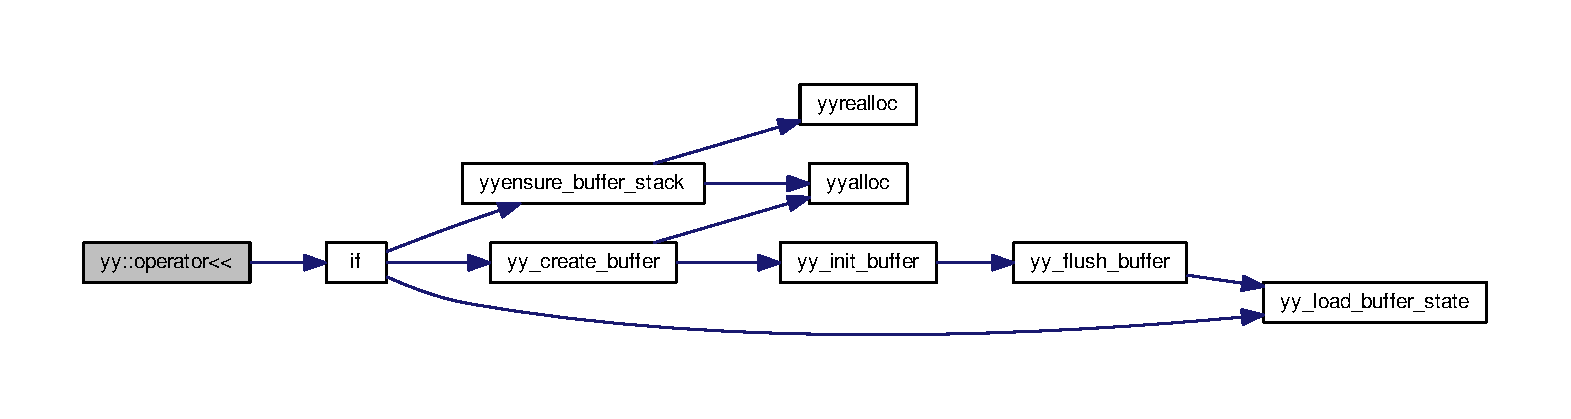
\includegraphics[width=350pt]{namespaceyy_a0406f2358d6ba6b06648ff66f3508aad_cgraph}
\end{center}
\end{figure}


\hypertarget{namespaceyy_a30a61b0569cd2c9ea4ae16eb4994c7b3}{\index{yy@{yy}!operator==@{operator==}}
\index{operator==@{operator==}!yy@{yy}}
\subsubsection[{operator==}]{\setlength{\rightskip}{0pt plus 5cm}bool yy\-::operator== (
\begin{DoxyParamCaption}
\item[{const position \&}]{pos1, }
\item[{const position \&}]{pos2}
\end{DoxyParamCaption}
)\hspace{0.3cm}{\ttfamily [inline]}}}\label{namespaceyy_a30a61b0569cd2c9ea4ae16eb4994c7b3}


Compare two position objects. 



Definition at line 145 of file position.\-hh.

\hypertarget{namespaceyy_a466b6e3dcf6a743bb058bf4989b38047}{\index{yy@{yy}!operator==@{operator==}}
\index{operator==@{operator==}!yy@{yy}}
\subsubsection[{operator==}]{\setlength{\rightskip}{0pt plus 5cm}bool yy\-::operator== (
\begin{DoxyParamCaption}
\item[{const location \&}]{loc1, }
\item[{const location \&}]{loc2}
\end{DoxyParamCaption}
)\hspace{0.3cm}{\ttfamily [inline]}}}\label{namespaceyy_a466b6e3dcf6a743bb058bf4989b38047}


Compare two location objects. 



Definition at line 151 of file location.\-hh.


\chapter{Class Documentation}
\hypertarget{class_assign}{}\section{Assign Class Reference}
\label{class_assign}\index{Assign@{Assign}}


{\ttfamily \#include $<$Assign.\+h$>$}



Inheritance diagram for Assign\+:
\nopagebreak
\begin{figure}[H]
\begin{center}
\leavevmode
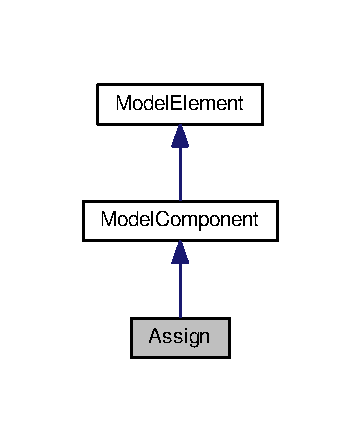
\includegraphics[width=181pt]{class_assign__inherit__graph}
\end{center}
\end{figure}


Collaboration diagram for Assign\+:
\nopagebreak
\begin{figure}[H]
\begin{center}
\leavevmode
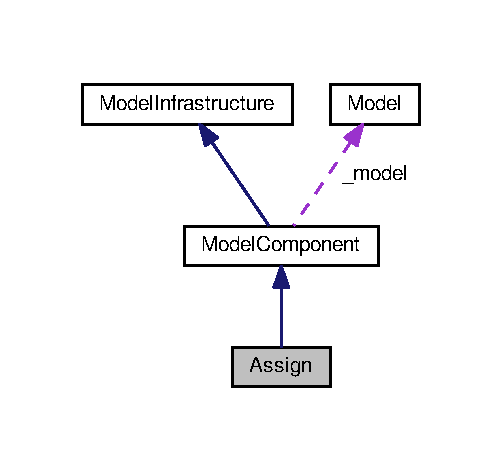
\includegraphics[width=242pt]{class_assign__coll__graph}
\end{center}
\end{figure}
\subsection*{Classes}
\begin{DoxyCompactItemize}
\item 
class \hyperlink{class_assign_1_1_assignment}{Assignment}
\end{DoxyCompactItemize}
\subsection*{Public Types}
\begin{DoxyCompactItemize}
\item 
enum \hyperlink{class_assign_ae0f42117c12a8d0bc2bf0b7574070694}{Destination\+Type} \{ \hyperlink{class_assign_ae0f42117c12a8d0bc2bf0b7574070694af2bbdf9f72c085adc4d0404e370f0f4c}{Destination\+Type\+::\+Attribute}, 
\hyperlink{class_assign_ae0f42117c12a8d0bc2bf0b7574070694a47c14840d8e15331fa420b9b2f757cd9}{Destination\+Type\+::\+Variable}
 \}
\end{DoxyCompactItemize}
\subsection*{Public Member Functions}
\begin{DoxyCompactItemize}
\item 
\hyperlink{class_assign_afaa746a0ce157d4606823ad508dc6281}{Assign} (\hyperlink{class_model}{Model} $\ast$model)
\item 
\hyperlink{class_assign_ae4945adcf1b5dcdd3f57faa9dd85a2b0}{Assign} (const \hyperlink{class_assign}{Assign} \&orig)
\item 
virtual \hyperlink{class_assign_aa005626af06022d9101c5e38e794dc47}{$\sim$\+Assign} ()
\item 
virtual std\+::string \hyperlink{class_assign_af5022b92204adcd9ee3e444b7e316d07}{show} ()
\item 
\hyperlink{class_list}{List}$<$ \hyperlink{class_assign_1_1_assignment}{Assignment} $\ast$ $>$ $\ast$ \hyperlink{class_assign_aca4aaa2185cc8770e56e1b6928c33dc0}{get\+Assignments} () const 
\end{DoxyCompactItemize}
\subsection*{Protected Member Functions}
\begin{DoxyCompactItemize}
\item 
virtual void \hyperlink{class_assign_a5fabf69268b2e65d8b01ce247be87a40}{\+\_\+execute} (\hyperlink{class_entity}{Entity} $\ast$entity)
\item 
virtual void \hyperlink{class_assign_a95e3169a6ae13ef3dc6dd9f0dde16c30}{\+\_\+load\+Instance} (std\+::list$<$ std\+::string $>$ words)
\item 
virtual std\+::list$<$ std\+::string $>$ $\ast$ \hyperlink{class_assign_a8b38a0a1bec283f5d2f44f67be5a4a6b}{\+\_\+save\+Instance} ()
\item 
virtual bool \hyperlink{class_assign_a5f3a7d8a7214574fea926cae1b1acb94}{\+\_\+verify\+Symbols} (std\+::string $\ast$error\+Message)
\end{DoxyCompactItemize}
\subsection*{Additional Inherited Members}


\subsection{Member Enumeration Documentation}
\index{Assign@{Assign}!Destination\+Type@{Destination\+Type}}
\index{Destination\+Type@{Destination\+Type}!Assign@{Assign}}
\subsubsection[{\texorpdfstring{Destination\+Type}{DestinationType}}]{\setlength{\rightskip}{0pt plus 5cm}enum {\bf Assign\+::\+Destination\+Type}\hspace{0.3cm}{\ttfamily [strong]}}\hypertarget{class_assign_ae0f42117c12a8d0bc2bf0b7574070694}{}\label{class_assign_ae0f42117c12a8d0bc2bf0b7574070694}
\begin{Desc}
\item[Enumerator]\par
\begin{description}
\index{Attribute@{Attribute}!Assign@{Assign}}\index{Assign@{Assign}!Attribute@{Attribute}}\item[{\em 
Attribute\hypertarget{class_assign_ae0f42117c12a8d0bc2bf0b7574070694af2bbdf9f72c085adc4d0404e370f0f4c}{}\label{class_assign_ae0f42117c12a8d0bc2bf0b7574070694af2bbdf9f72c085adc4d0404e370f0f4c}
}]\index{Variable@{Variable}!Assign@{Assign}}\index{Assign@{Assign}!Variable@{Variable}}\item[{\em 
Variable\hypertarget{class_assign_ae0f42117c12a8d0bc2bf0b7574070694a47c14840d8e15331fa420b9b2f757cd9}{}\label{class_assign_ae0f42117c12a8d0bc2bf0b7574070694a47c14840d8e15331fa420b9b2f757cd9}
}]\end{description}
\end{Desc}


\subsection{Constructor \& Destructor Documentation}
\index{Assign@{Assign}!Assign@{Assign}}
\index{Assign@{Assign}!Assign@{Assign}}
\subsubsection[{\texorpdfstring{Assign(\+Model $\ast$model)}{Assign(Model *model)}}]{\setlength{\rightskip}{0pt plus 5cm}Assign\+::\+Assign (
\begin{DoxyParamCaption}
\item[{{\bf Model} $\ast$}]{model}
\end{DoxyParamCaption}
)}\hypertarget{class_assign_afaa746a0ce157d4606823ad508dc6281}{}\label{class_assign_afaa746a0ce157d4606823ad508dc6281}
\index{Assign@{Assign}!Assign@{Assign}}
\index{Assign@{Assign}!Assign@{Assign}}
\subsubsection[{\texorpdfstring{Assign(const Assign \&orig)}{Assign(const Assign &orig)}}]{\setlength{\rightskip}{0pt plus 5cm}Assign\+::\+Assign (
\begin{DoxyParamCaption}
\item[{const {\bf Assign} \&}]{orig}
\end{DoxyParamCaption}
)}\hypertarget{class_assign_ae4945adcf1b5dcdd3f57faa9dd85a2b0}{}\label{class_assign_ae4945adcf1b5dcdd3f57faa9dd85a2b0}
\index{Assign@{Assign}!````~Assign@{$\sim$\+Assign}}
\index{````~Assign@{$\sim$\+Assign}!Assign@{Assign}}
\subsubsection[{\texorpdfstring{$\sim$\+Assign()}{~Assign()}}]{\setlength{\rightskip}{0pt plus 5cm}Assign\+::$\sim$\+Assign (
\begin{DoxyParamCaption}
{}
\end{DoxyParamCaption}
)\hspace{0.3cm}{\ttfamily [virtual]}}\hypertarget{class_assign_aa005626af06022d9101c5e38e794dc47}{}\label{class_assign_aa005626af06022d9101c5e38e794dc47}


\subsection{Member Function Documentation}
\index{Assign@{Assign}!\+\_\+execute@{\+\_\+execute}}
\index{\+\_\+execute@{\+\_\+execute}!Assign@{Assign}}
\subsubsection[{\texorpdfstring{\+\_\+execute(\+Entity $\ast$entity)}{_execute(Entity *entity)}}]{\setlength{\rightskip}{0pt plus 5cm}void Assign\+::\+\_\+execute (
\begin{DoxyParamCaption}
\item[{{\bf Entity} $\ast$}]{entity}
\end{DoxyParamCaption}
)\hspace{0.3cm}{\ttfamily [protected]}, {\ttfamily [virtual]}}\hypertarget{class_assign_a5fabf69268b2e65d8b01ce247be87a40}{}\label{class_assign_a5fabf69268b2e65d8b01ce247be87a40}


Implements \hyperlink{class_model_component_ae3fcf8bbdd8368c882438424aa73f714}{Model\+Component}.

\index{Assign@{Assign}!\+\_\+load\+Instance@{\+\_\+load\+Instance}}
\index{\+\_\+load\+Instance@{\+\_\+load\+Instance}!Assign@{Assign}}
\subsubsection[{\texorpdfstring{\+\_\+load\+Instance(std\+::list$<$ std\+::string $>$ words)}{_loadInstance(std::list< std::string > words)}}]{\setlength{\rightskip}{0pt plus 5cm}void Assign\+::\+\_\+load\+Instance (
\begin{DoxyParamCaption}
\item[{std\+::list$<$ std\+::string $>$}]{words}
\end{DoxyParamCaption}
)\hspace{0.3cm}{\ttfamily [protected]}, {\ttfamily [virtual]}}\hypertarget{class_assign_a95e3169a6ae13ef3dc6dd9f0dde16c30}{}\label{class_assign_a95e3169a6ae13ef3dc6dd9f0dde16c30}


Implements \hyperlink{class_model_infrastructure_ae118c8ad2ac9d4397c40d004af51b2dc}{Model\+Infrastructure}.

\index{Assign@{Assign}!\+\_\+save\+Instance@{\+\_\+save\+Instance}}
\index{\+\_\+save\+Instance@{\+\_\+save\+Instance}!Assign@{Assign}}
\subsubsection[{\texorpdfstring{\+\_\+save\+Instance()}{_saveInstance()}}]{\setlength{\rightskip}{0pt plus 5cm}std\+::list$<$ std\+::string $>$ $\ast$ Assign\+::\+\_\+save\+Instance (
\begin{DoxyParamCaption}
{}
\end{DoxyParamCaption}
)\hspace{0.3cm}{\ttfamily [protected]}, {\ttfamily [virtual]}}\hypertarget{class_assign_a8b38a0a1bec283f5d2f44f67be5a4a6b}{}\label{class_assign_a8b38a0a1bec283f5d2f44f67be5a4a6b}


Reimplemented from \hyperlink{class_model_component_a465f41c7191cb0fdf9039ef1f3d755a5}{Model\+Component}.

\index{Assign@{Assign}!\+\_\+verify\+Symbols@{\+\_\+verify\+Symbols}}
\index{\+\_\+verify\+Symbols@{\+\_\+verify\+Symbols}!Assign@{Assign}}
\subsubsection[{\texorpdfstring{\+\_\+verify\+Symbols(std\+::string $\ast$error\+Message)}{_verifySymbols(std::string *errorMessage)}}]{\setlength{\rightskip}{0pt plus 5cm}bool Assign\+::\+\_\+verify\+Symbols (
\begin{DoxyParamCaption}
\item[{std\+::string $\ast$}]{error\+Message}
\end{DoxyParamCaption}
)\hspace{0.3cm}{\ttfamily [protected]}, {\ttfamily [virtual]}}\hypertarget{class_assign_a5f3a7d8a7214574fea926cae1b1acb94}{}\label{class_assign_a5f3a7d8a7214574fea926cae1b1acb94}


Implements \hyperlink{class_model_infrastructure_a43de089b35b96c32dd24ca4f9636a388}{Model\+Infrastructure}.

\index{Assign@{Assign}!get\+Assignments@{get\+Assignments}}
\index{get\+Assignments@{get\+Assignments}!Assign@{Assign}}
\subsubsection[{\texorpdfstring{get\+Assignments() const }{getAssignments() const }}]{\setlength{\rightskip}{0pt plus 5cm}{\bf List}$<$ {\bf Assign\+::\+Assignment} $\ast$ $>$ $\ast$ Assign\+::get\+Assignments (
\begin{DoxyParamCaption}
{}
\end{DoxyParamCaption}
) const}\hypertarget{class_assign_aca4aaa2185cc8770e56e1b6928c33dc0}{}\label{class_assign_aca4aaa2185cc8770e56e1b6928c33dc0}
\index{Assign@{Assign}!show@{show}}
\index{show@{show}!Assign@{Assign}}
\subsubsection[{\texorpdfstring{show()}{show()}}]{\setlength{\rightskip}{0pt plus 5cm}std\+::string Assign\+::show (
\begin{DoxyParamCaption}
{}
\end{DoxyParamCaption}
)\hspace{0.3cm}{\ttfamily [virtual]}}\hypertarget{class_assign_af5022b92204adcd9ee3e444b7e316d07}{}\label{class_assign_af5022b92204adcd9ee3e444b7e316d07}


Reimplemented from \hyperlink{class_model_component_ad8bc846e36b028eab7efb7da6c549eca}{Model\+Component}.



The documentation for this class was generated from the following files\+:\begin{DoxyCompactItemize}
\item 
\hyperlink{_assign_8h}{Assign.\+h}\item 
\hyperlink{_assign_8cpp}{Assign.\+cpp}\end{DoxyCompactItemize}

\hypertarget{class_assign_1_1_assignment}{}\section{Assign\+:\+:Assignment Class Reference}
\label{class_assign_1_1_assignment}\index{Assign\+::\+Assignment@{Assign\+::\+Assignment}}


{\ttfamily \#include $<$Assign.\+h$>$}

\subsection*{Public Member Functions}
\begin{DoxyCompactItemize}
\item 
\hyperlink{class_assign_1_1_assignment_a41583f4bbce99b1d95f4ef067c236f7a}{Assignment} (\hyperlink{class_assign_ae0f42117c12a8d0bc2bf0b7574070694}{Destination\+Type} destination\+Type, std\+::string destination, std\+::string expression)
\item 
void \hyperlink{class_assign_1_1_assignment_a8d0c9b18c0b1258bba905b4e47a2659b}{set\+Destination} (std\+::string \+\_\+destination)
\item 
std\+::string \hyperlink{class_assign_1_1_assignment_a6cf7ecd2950dfc709985a1ede3773be8}{get\+Destination} () const 
\item 
void \hyperlink{class_assign_1_1_assignment_a9688ea3171c85ccbcdf0ed9d87ad9cc7}{set\+Destination\+Type} (\hyperlink{class_assign_ae0f42117c12a8d0bc2bf0b7574070694}{Destination\+Type} \+\_\+destination\+Type)
\item 
\hyperlink{class_assign_ae0f42117c12a8d0bc2bf0b7574070694}{Destination\+Type} \hyperlink{class_assign_1_1_assignment_a46493b98c1cd97ce4b015640bf34dd27}{get\+Destination\+Type} () const 
\item 
void \hyperlink{class_assign_1_1_assignment_aa36ca609362d3deedffbefd9cceb12e6}{set\+Expression} (std\+::string \+\_\+expression)
\item 
std\+::string \hyperlink{class_assign_1_1_assignment_a724dc03a686c4d53d57ee45b7617ae2f}{get\+Expression} () const 
\end{DoxyCompactItemize}


\subsection{Constructor \& Destructor Documentation}
\index{Assign\+::\+Assignment@{Assign\+::\+Assignment}!Assignment@{Assignment}}
\index{Assignment@{Assignment}!Assign\+::\+Assignment@{Assign\+::\+Assignment}}
\subsubsection[{\texorpdfstring{Assignment(\+Destination\+Type destination\+Type, std\+::string destination, std\+::string expression)}{Assignment(DestinationType destinationType, std::string destination, std::string expression)}}]{\setlength{\rightskip}{0pt plus 5cm}Assign\+::\+Assignment\+::\+Assignment (
\begin{DoxyParamCaption}
\item[{{\bf Destination\+Type}}]{destination\+Type, }
\item[{std\+::string}]{destination, }
\item[{std\+::string}]{expression}
\end{DoxyParamCaption}
)\hspace{0.3cm}{\ttfamily [inline]}}\hypertarget{class_assign_1_1_assignment_a41583f4bbce99b1d95f4ef067c236f7a}{}\label{class_assign_1_1_assignment_a41583f4bbce99b1d95f4ef067c236f7a}


\subsection{Member Function Documentation}
\index{Assign\+::\+Assignment@{Assign\+::\+Assignment}!get\+Destination@{get\+Destination}}
\index{get\+Destination@{get\+Destination}!Assign\+::\+Assignment@{Assign\+::\+Assignment}}
\subsubsection[{\texorpdfstring{get\+Destination() const }{getDestination() const }}]{\setlength{\rightskip}{0pt plus 5cm}std\+::string Assign\+::\+Assignment\+::get\+Destination (
\begin{DoxyParamCaption}
{}
\end{DoxyParamCaption}
) const\hspace{0.3cm}{\ttfamily [inline]}}\hypertarget{class_assign_1_1_assignment_a6cf7ecd2950dfc709985a1ede3773be8}{}\label{class_assign_1_1_assignment_a6cf7ecd2950dfc709985a1ede3773be8}
\index{Assign\+::\+Assignment@{Assign\+::\+Assignment}!get\+Destination\+Type@{get\+Destination\+Type}}
\index{get\+Destination\+Type@{get\+Destination\+Type}!Assign\+::\+Assignment@{Assign\+::\+Assignment}}
\subsubsection[{\texorpdfstring{get\+Destination\+Type() const }{getDestinationType() const }}]{\setlength{\rightskip}{0pt plus 5cm}{\bf Destination\+Type} Assign\+::\+Assignment\+::get\+Destination\+Type (
\begin{DoxyParamCaption}
{}
\end{DoxyParamCaption}
) const\hspace{0.3cm}{\ttfamily [inline]}}\hypertarget{class_assign_1_1_assignment_a46493b98c1cd97ce4b015640bf34dd27}{}\label{class_assign_1_1_assignment_a46493b98c1cd97ce4b015640bf34dd27}
\index{Assign\+::\+Assignment@{Assign\+::\+Assignment}!get\+Expression@{get\+Expression}}
\index{get\+Expression@{get\+Expression}!Assign\+::\+Assignment@{Assign\+::\+Assignment}}
\subsubsection[{\texorpdfstring{get\+Expression() const }{getExpression() const }}]{\setlength{\rightskip}{0pt plus 5cm}std\+::string Assign\+::\+Assignment\+::get\+Expression (
\begin{DoxyParamCaption}
{}
\end{DoxyParamCaption}
) const\hspace{0.3cm}{\ttfamily [inline]}}\hypertarget{class_assign_1_1_assignment_a724dc03a686c4d53d57ee45b7617ae2f}{}\label{class_assign_1_1_assignment_a724dc03a686c4d53d57ee45b7617ae2f}
\index{Assign\+::\+Assignment@{Assign\+::\+Assignment}!set\+Destination@{set\+Destination}}
\index{set\+Destination@{set\+Destination}!Assign\+::\+Assignment@{Assign\+::\+Assignment}}
\subsubsection[{\texorpdfstring{set\+Destination(std\+::string \+\_\+destination)}{setDestination(std::string _destination)}}]{\setlength{\rightskip}{0pt plus 5cm}void Assign\+::\+Assignment\+::set\+Destination (
\begin{DoxyParamCaption}
\item[{std\+::string}]{\+\_\+destination}
\end{DoxyParamCaption}
)\hspace{0.3cm}{\ttfamily [inline]}}\hypertarget{class_assign_1_1_assignment_a8d0c9b18c0b1258bba905b4e47a2659b}{}\label{class_assign_1_1_assignment_a8d0c9b18c0b1258bba905b4e47a2659b}
\index{Assign\+::\+Assignment@{Assign\+::\+Assignment}!set\+Destination\+Type@{set\+Destination\+Type}}
\index{set\+Destination\+Type@{set\+Destination\+Type}!Assign\+::\+Assignment@{Assign\+::\+Assignment}}
\subsubsection[{\texorpdfstring{set\+Destination\+Type(\+Destination\+Type \+\_\+destination\+Type)}{setDestinationType(DestinationType _destinationType)}}]{\setlength{\rightskip}{0pt plus 5cm}void Assign\+::\+Assignment\+::set\+Destination\+Type (
\begin{DoxyParamCaption}
\item[{{\bf Destination\+Type}}]{\+\_\+destination\+Type}
\end{DoxyParamCaption}
)\hspace{0.3cm}{\ttfamily [inline]}}\hypertarget{class_assign_1_1_assignment_a9688ea3171c85ccbcdf0ed9d87ad9cc7}{}\label{class_assign_1_1_assignment_a9688ea3171c85ccbcdf0ed9d87ad9cc7}
\index{Assign\+::\+Assignment@{Assign\+::\+Assignment}!set\+Expression@{set\+Expression}}
\index{set\+Expression@{set\+Expression}!Assign\+::\+Assignment@{Assign\+::\+Assignment}}
\subsubsection[{\texorpdfstring{set\+Expression(std\+::string \+\_\+expression)}{setExpression(std::string _expression)}}]{\setlength{\rightskip}{0pt plus 5cm}void Assign\+::\+Assignment\+::set\+Expression (
\begin{DoxyParamCaption}
\item[{std\+::string}]{\+\_\+expression}
\end{DoxyParamCaption}
)\hspace{0.3cm}{\ttfamily [inline]}}\hypertarget{class_assign_1_1_assignment_aa36ca609362d3deedffbefd9cceb12e6}{}\label{class_assign_1_1_assignment_aa36ca609362d3deedffbefd9cceb12e6}


The documentation for this class was generated from the following file\+:\begin{DoxyCompactItemize}
\item 
\hyperlink{_assign_8h}{Assign.\+h}\end{DoxyCompactItemize}

\hypertarget{class_attribute}{\section{Attribute Class Reference}
\label{class_attribute}\index{Attribute@{Attribute}}
}


{\ttfamily \#include $<$Attribute.\-h$>$}



Inheritance diagram for Attribute\-:
\nopagebreak
\begin{figure}[H]
\begin{center}
\leavevmode
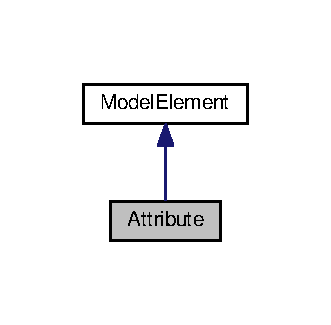
\includegraphics[width=180pt]{class_attribute__inherit__graph}
\end{center}
\end{figure}


Collaboration diagram for Attribute\-:
\nopagebreak
\begin{figure}[H]
\begin{center}
\leavevmode
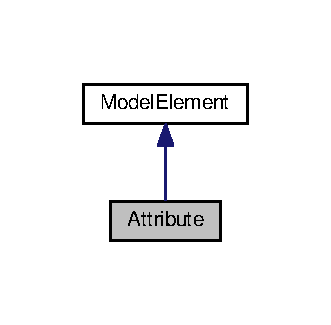
\includegraphics[width=180pt]{class_attribute__coll__graph}
\end{center}
\end{figure}
\subsection*{Public Member Functions}
\begin{DoxyCompactItemize}
\item 
\hyperlink{class_attribute_a8ba4e5a507aef352563e1e56f1930e66}{Attribute} ()
\item 
\hyperlink{class_attribute_a8a0c53bda9cc94180f06bda254809261}{Attribute} (const \hyperlink{class_attribute}{Attribute} \&orig)
\item 
virtual \hyperlink{class_attribute_a28ab087bb886728670e4ae5791bc2ea8}{$\sim$\-Attribute} ()
\item 
virtual std\-::string \hyperlink{class_attribute_aa29f79466bd6ed5e36c402ec57cb2050}{show} ()
\end{DoxyCompactItemize}
\subsection*{Protected Member Functions}
\begin{DoxyCompactItemize}
\item 
virtual void \hyperlink{class_attribute_ac76d3302ec24a4cca1e84fed221cf917}{\-\_\-load\-Instance} (std\-::list$<$ std\-::string $>$ words)
\item 
virtual std\-::list$<$ std\-::string $>$ $\ast$ \hyperlink{class_attribute_a32bd3d820fa2957d4a5d8c98db5b50e0}{\-\_\-save\-Instance} ()
\item 
virtual bool \hyperlink{class_attribute_adbe1f438203db4e87b0c8e1cd5e0182d}{\-\_\-verify\-Symbols} (std\-::string $\ast$error\-Message)
\end{DoxyCompactItemize}
\subsection*{Additional Inherited Members}


\subsection{Detailed Description}


Definition at line 24 of file Attribute.\-h.



\subsection{Constructor \& Destructor Documentation}
\hypertarget{class_attribute_a8ba4e5a507aef352563e1e56f1930e66}{\index{Attribute@{Attribute}!Attribute@{Attribute}}
\index{Attribute@{Attribute}!Attribute@{Attribute}}
\subsubsection[{Attribute}]{\setlength{\rightskip}{0pt plus 5cm}Attribute\-::\-Attribute (
\begin{DoxyParamCaption}
{}
\end{DoxyParamCaption}
)}}\label{class_attribute_a8ba4e5a507aef352563e1e56f1930e66}


Definition at line 16 of file Attribute.\-cpp.

\hypertarget{class_attribute_a8a0c53bda9cc94180f06bda254809261}{\index{Attribute@{Attribute}!Attribute@{Attribute}}
\index{Attribute@{Attribute}!Attribute@{Attribute}}
\subsubsection[{Attribute}]{\setlength{\rightskip}{0pt plus 5cm}Attribute\-::\-Attribute (
\begin{DoxyParamCaption}
\item[{const {\bf Attribute} \&}]{orig}
\end{DoxyParamCaption}
)}}\label{class_attribute_a8a0c53bda9cc94180f06bda254809261}


Definition at line 19 of file Attribute.\-cpp.

\hypertarget{class_attribute_a28ab087bb886728670e4ae5791bc2ea8}{\index{Attribute@{Attribute}!$\sim$\-Attribute@{$\sim$\-Attribute}}
\index{$\sim$\-Attribute@{$\sim$\-Attribute}!Attribute@{Attribute}}
\subsubsection[{$\sim$\-Attribute}]{\setlength{\rightskip}{0pt plus 5cm}Attribute\-::$\sim$\-Attribute (
\begin{DoxyParamCaption}
{}
\end{DoxyParamCaption}
)\hspace{0.3cm}{\ttfamily [virtual]}}}\label{class_attribute_a28ab087bb886728670e4ae5791bc2ea8}


Definition at line 22 of file Attribute.\-cpp.



\subsection{Member Function Documentation}
\hypertarget{class_attribute_ac76d3302ec24a4cca1e84fed221cf917}{\index{Attribute@{Attribute}!\-\_\-load\-Instance@{\-\_\-load\-Instance}}
\index{\-\_\-load\-Instance@{\-\_\-load\-Instance}!Attribute@{Attribute}}
\subsubsection[{\-\_\-load\-Instance}]{\setlength{\rightskip}{0pt plus 5cm}void Attribute\-::\-\_\-load\-Instance (
\begin{DoxyParamCaption}
\item[{std\-::list$<$ std\-::string $>$}]{words}
\end{DoxyParamCaption}
)\hspace{0.3cm}{\ttfamily [protected]}, {\ttfamily [virtual]}}}\label{class_attribute_ac76d3302ec24a4cca1e84fed221cf917}


Implements \hyperlink{class_model_infrastructure_ae118c8ad2ac9d4397c40d004af51b2dc}{Model\-Infrastructure}.



Definition at line 29 of file Attribute.\-cpp.

\hypertarget{class_attribute_a32bd3d820fa2957d4a5d8c98db5b50e0}{\index{Attribute@{Attribute}!\-\_\-save\-Instance@{\-\_\-save\-Instance}}
\index{\-\_\-save\-Instance@{\-\_\-save\-Instance}!Attribute@{Attribute}}
\subsubsection[{\-\_\-save\-Instance}]{\setlength{\rightskip}{0pt plus 5cm}std\-::list$<$ std\-::string $>$ $\ast$ Attribute\-::\-\_\-save\-Instance (
\begin{DoxyParamCaption}
{}
\end{DoxyParamCaption}
)\hspace{0.3cm}{\ttfamily [protected]}, {\ttfamily [virtual]}}}\label{class_attribute_a32bd3d820fa2957d4a5d8c98db5b50e0}


Implements \hyperlink{class_model_infrastructure_a3da2fd381c44752598bc448b207e8287}{Model\-Infrastructure}.



Definition at line 32 of file Attribute.\-cpp.

\hypertarget{class_attribute_adbe1f438203db4e87b0c8e1cd5e0182d}{\index{Attribute@{Attribute}!\-\_\-verify\-Symbols@{\-\_\-verify\-Symbols}}
\index{\-\_\-verify\-Symbols@{\-\_\-verify\-Symbols}!Attribute@{Attribute}}
\subsubsection[{\-\_\-verify\-Symbols}]{\setlength{\rightskip}{0pt plus 5cm}bool Attribute\-::\-\_\-verify\-Symbols (
\begin{DoxyParamCaption}
\item[{std\-::string $\ast$}]{error\-Message}
\end{DoxyParamCaption}
)\hspace{0.3cm}{\ttfamily [protected]}, {\ttfamily [virtual]}}}\label{class_attribute_adbe1f438203db4e87b0c8e1cd5e0182d}


Implements \hyperlink{class_model_infrastructure_a43de089b35b96c32dd24ca4f9636a388}{Model\-Infrastructure}.



Definition at line 37 of file Attribute.\-cpp.

\hypertarget{class_attribute_aa29f79466bd6ed5e36c402ec57cb2050}{\index{Attribute@{Attribute}!show@{show}}
\index{show@{show}!Attribute@{Attribute}}
\subsubsection[{show}]{\setlength{\rightskip}{0pt plus 5cm}std\-::string Attribute\-::show (
\begin{DoxyParamCaption}
{}
\end{DoxyParamCaption}
)\hspace{0.3cm}{\ttfamily [virtual]}}}\label{class_attribute_aa29f79466bd6ed5e36c402ec57cb2050}


Reimplemented from \hyperlink{class_model_infrastructure_a649a5a89a0c9931783d3c51de2acf266}{Model\-Infrastructure}.



Definition at line 25 of file Attribute.\-cpp.



Here is the call graph for this function\-:
\nopagebreak
\begin{figure}[H]
\begin{center}
\leavevmode
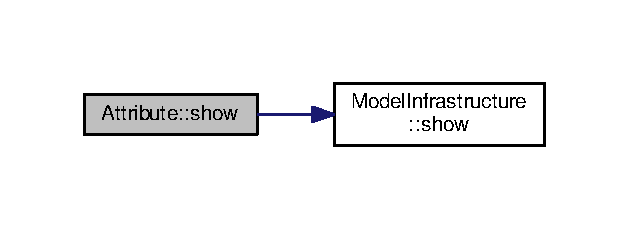
\includegraphics[width=302pt]{class_attribute_aa29f79466bd6ed5e36c402ec57cb2050_cgraph}
\end{center}
\end{figure}




The documentation for this class was generated from the following files\-:\begin{DoxyCompactItemize}
\item 
\hyperlink{_attribute_8h}{Attribute.\-h}\item 
\hyperlink{_attribute_8cpp}{Attribute.\-cpp}\end{DoxyCompactItemize}

\hypertarget{structyy_1_1genesyspp__parser_1_1basic__symbol}{\section{yy\-:\-:genesyspp\-\_\-parser\-:\-:basic\-\_\-symbol$<$ Base $>$ Struct Template Reference}
\label{structyy_1_1genesyspp__parser_1_1basic__symbol}\index{yy\-::genesyspp\-\_\-parser\-::basic\-\_\-symbol$<$ Base $>$@{yy\-::genesyspp\-\_\-parser\-::basic\-\_\-symbol$<$ Base $>$}}
}


{\ttfamily \#include $<$Genesys++-\/parser.\-h$>$}



Inheritance diagram for yy\-:\-:genesyspp\-\_\-parser\-:\-:basic\-\_\-symbol$<$ Base $>$\-:
\nopagebreak
\begin{figure}[H]
\begin{center}
\leavevmode
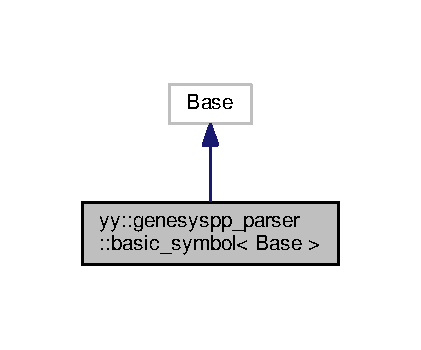
\includegraphics[width=202pt]{structyy_1_1genesyspp__parser_1_1basic__symbol__inherit__graph}
\end{center}
\end{figure}


Collaboration diagram for yy\-:\-:genesyspp\-\_\-parser\-:\-:basic\-\_\-symbol$<$ Base $>$\-:
\nopagebreak
\begin{figure}[H]
\begin{center}
\leavevmode
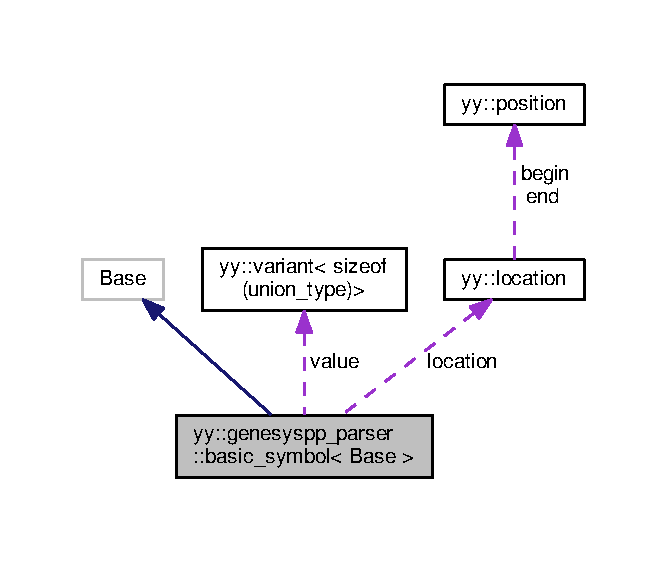
\includegraphics[width=320pt]{structyy_1_1genesyspp__parser_1_1basic__symbol__coll__graph}
\end{center}
\end{figure}
\subsection*{Public Types}
\begin{DoxyCompactItemize}
\item 
typedef Base \hyperlink{structyy_1_1genesyspp__parser_1_1basic__symbol_a1493afba8ed8b978a445fa2cb8b57867}{super\-\_\-type}
\begin{DoxyCompactList}\small\item\em Alias to Base. \end{DoxyCompactList}\end{DoxyCompactItemize}
\subsection*{Public Member Functions}
\begin{DoxyCompactItemize}
\item 
\hyperlink{structyy_1_1genesyspp__parser_1_1basic__symbol_ac749c8aa9c095dca4f6455cb91c8a90d}{basic\-\_\-symbol} ()
\begin{DoxyCompactList}\small\item\em Default constructor. \end{DoxyCompactList}\item 
\hyperlink{structyy_1_1genesyspp__parser_1_1basic__symbol_a9675a48bfdda3c3c4d3937124740dac4}{basic\-\_\-symbol} (const \hyperlink{structyy_1_1genesyspp__parser_1_1basic__symbol}{basic\-\_\-symbol} \&other)
\begin{DoxyCompactList}\small\item\em Copy constructor. \end{DoxyCompactList}\item 
\hyperlink{structyy_1_1genesyspp__parser_1_1basic__symbol_a9f10b31e1972d8e8956baff9aa2640e9}{basic\-\_\-symbol} (typename Base\-::kind\-\_\-type t, const \hyperlink{classyy_1_1genesyspp__parser_aa0276d3782ebff157827ad5e7d44f97c}{location\-\_\-type} \&l)
\begin{DoxyCompactList}\small\item\em Constructor for valueless symbols, and symbols from each type. \end{DoxyCompactList}\item 
\hyperlink{structyy_1_1genesyspp__parser_1_1basic__symbol_af2a91dccb375a9bc1fb9bb11c7d5907d}{basic\-\_\-symbol} (typename Base\-::kind\-\_\-type t, const \hyperlink{classobj__t}{obj\-\_\-t} \&v, const \hyperlink{classyy_1_1genesyspp__parser_aa0276d3782ebff157827ad5e7d44f97c}{location\-\_\-type} \&l)
\item 
\hyperlink{structyy_1_1genesyspp__parser_1_1basic__symbol_a94529fa808d843d97fad2b531bd04466}{basic\-\_\-symbol} (typename Base\-::kind\-\_\-type t, const \hyperlink{classyy_1_1genesyspp__parser_a592978b9aaaa0d61f9faf4093f5f554d}{semantic\-\_\-type} \&v, const \hyperlink{classyy_1_1genesyspp__parser_aa0276d3782ebff157827ad5e7d44f97c}{location\-\_\-type} \&l)
\begin{DoxyCompactList}\small\item\em Constructor for symbols with semantic value. \end{DoxyCompactList}\item 
\hyperlink{structyy_1_1genesyspp__parser_1_1basic__symbol_aeaa054339c41c834ec30bbda4dc3beff}{$\sim$basic\-\_\-symbol} ()
\begin{DoxyCompactList}\small\item\em Destroy the symbol. \end{DoxyCompactList}\item 
void \hyperlink{structyy_1_1genesyspp__parser_1_1basic__symbol_a307cece0deecd34ac5f4812a92d69d0b}{clear} ()
\begin{DoxyCompactList}\small\item\em Destroy contents, and record that is empty. \end{DoxyCompactList}\item 
bool \hyperlink{structyy_1_1genesyspp__parser_1_1basic__symbol_af31a4325622f49b9903cdc6734e4f9d8}{empty} () const 
\begin{DoxyCompactList}\small\item\em Whether empty. \end{DoxyCompactList}\item 
void \hyperlink{structyy_1_1genesyspp__parser_1_1basic__symbol_a4244f8c6794d7869a9e82a96cd49e5f2}{move} (\hyperlink{structyy_1_1genesyspp__parser_1_1basic__symbol}{basic\-\_\-symbol} \&s)
\begin{DoxyCompactList}\small\item\em Destructive move, {\itshape s} is emptied into this. \end{DoxyCompactList}\end{DoxyCompactItemize}
\subsection*{Public Attributes}
\begin{DoxyCompactItemize}
\item 
\hyperlink{classyy_1_1genesyspp__parser_a592978b9aaaa0d61f9faf4093f5f554d}{semantic\-\_\-type} \hyperlink{structyy_1_1genesyspp__parser_1_1basic__symbol_a66fa4a750b9ae7e8be9c640b8712fe0b}{value}
\begin{DoxyCompactList}\small\item\em The semantic value. \end{DoxyCompactList}\item 
\hyperlink{classyy_1_1genesyspp__parser_aa0276d3782ebff157827ad5e7d44f97c}{location\-\_\-type} \hyperlink{structyy_1_1genesyspp__parser_1_1basic__symbol_ae95666bbb377d80e31b8a676aa44e84a}{location}
\begin{DoxyCompactList}\small\item\em The location. \end{DoxyCompactList}\end{DoxyCompactItemize}


\subsection{Detailed Description}
\subsubsection*{template$<$typename Base$>$struct yy\-::genesyspp\-\_\-parser\-::basic\-\_\-symbol$<$ Base $>$}

A complete symbol.

Expects its Base type to provide access to the symbol type via type\-\_\-get().

Provide access to semantic value and location. 

Definition at line 480 of file Genesys++-\/parser.\-h.



\subsection{Member Typedef Documentation}
\hypertarget{structyy_1_1genesyspp__parser_1_1basic__symbol_a1493afba8ed8b978a445fa2cb8b57867}{\index{yy\-::genesyspp\-\_\-parser\-::basic\-\_\-symbol@{yy\-::genesyspp\-\_\-parser\-::basic\-\_\-symbol}!super\-\_\-type@{super\-\_\-type}}
\index{super\-\_\-type@{super\-\_\-type}!yy::genesyspp_parser::basic_symbol@{yy\-::genesyspp\-\_\-parser\-::basic\-\_\-symbol}}
\subsubsection[{super\-\_\-type}]{\setlength{\rightskip}{0pt plus 5cm}template$<$typename Base$>$ typedef Base {\bf yy\-::genesyspp\-\_\-parser\-::basic\-\_\-symbol}$<$ Base $>$\-::{\bf super\-\_\-type}}}\label{structyy_1_1genesyspp__parser_1_1basic__symbol_a1493afba8ed8b978a445fa2cb8b57867}


Alias to Base. 



Definition at line 483 of file Genesys++-\/parser.\-h.



\subsection{Constructor \& Destructor Documentation}
\hypertarget{structyy_1_1genesyspp__parser_1_1basic__symbol_ac749c8aa9c095dca4f6455cb91c8a90d}{\index{yy\-::genesyspp\-\_\-parser\-::basic\-\_\-symbol@{yy\-::genesyspp\-\_\-parser\-::basic\-\_\-symbol}!basic\-\_\-symbol@{basic\-\_\-symbol}}
\index{basic\-\_\-symbol@{basic\-\_\-symbol}!yy::genesyspp_parser::basic_symbol@{yy\-::genesyspp\-\_\-parser\-::basic\-\_\-symbol}}
\subsubsection[{basic\-\_\-symbol}]{\setlength{\rightskip}{0pt plus 5cm}template$<$typename Base $>$ {\bf yy\-::genesyspp\-\_\-parser\-::basic\-\_\-symbol}$<$ Base $>$\-::{\bf basic\-\_\-symbol} (
\begin{DoxyParamCaption}
{}
\end{DoxyParamCaption}
)}}\label{structyy_1_1genesyspp__parser_1_1basic__symbol_ac749c8aa9c095dca4f6455cb91c8a90d}


Default constructor. 



Definition at line 1077 of file Genesys++-\/parser.\-h.

\hypertarget{structyy_1_1genesyspp__parser_1_1basic__symbol_a9675a48bfdda3c3c4d3937124740dac4}{\index{yy\-::genesyspp\-\_\-parser\-::basic\-\_\-symbol@{yy\-::genesyspp\-\_\-parser\-::basic\-\_\-symbol}!basic\-\_\-symbol@{basic\-\_\-symbol}}
\index{basic\-\_\-symbol@{basic\-\_\-symbol}!yy::genesyspp_parser::basic_symbol@{yy\-::genesyspp\-\_\-parser\-::basic\-\_\-symbol}}
\subsubsection[{basic\-\_\-symbol}]{\setlength{\rightskip}{0pt plus 5cm}template$<$typename Base $>$ {\bf yy\-::genesyspp\-\_\-parser\-::basic\-\_\-symbol}$<$ Base $>$\-::{\bf basic\-\_\-symbol} (
\begin{DoxyParamCaption}
\item[{const {\bf basic\-\_\-symbol}$<$ Base $>$ \&}]{other}
\end{DoxyParamCaption}
)}}\label{structyy_1_1genesyspp__parser_1_1basic__symbol_a9675a48bfdda3c3c4d3937124740dac4}


Copy constructor. 



Definition at line 1083 of file Genesys++-\/parser.\-h.



Here is the call graph for this function\-:
\nopagebreak
\begin{figure}[H]
\begin{center}
\leavevmode
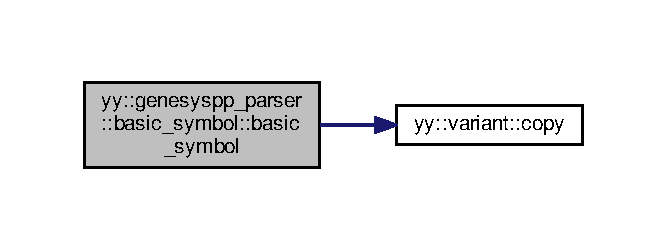
\includegraphics[width=320pt]{structyy_1_1genesyspp__parser_1_1basic__symbol_a9675a48bfdda3c3c4d3937124740dac4_cgraph}
\end{center}
\end{figure}


\hypertarget{structyy_1_1genesyspp__parser_1_1basic__symbol_a9f10b31e1972d8e8956baff9aa2640e9}{\index{yy\-::genesyspp\-\_\-parser\-::basic\-\_\-symbol@{yy\-::genesyspp\-\_\-parser\-::basic\-\_\-symbol}!basic\-\_\-symbol@{basic\-\_\-symbol}}
\index{basic\-\_\-symbol@{basic\-\_\-symbol}!yy::genesyspp_parser::basic_symbol@{yy\-::genesyspp\-\_\-parser\-::basic\-\_\-symbol}}
\subsubsection[{basic\-\_\-symbol}]{\setlength{\rightskip}{0pt plus 5cm}template$<$typename Base$>$ {\bf yy\-::genesyspp\-\_\-parser\-::basic\-\_\-symbol}$<$ Base $>$\-::{\bf basic\-\_\-symbol} (
\begin{DoxyParamCaption}
\item[{typename Base\-::kind\-\_\-type}]{t, }
\item[{const {\bf location\-\_\-type} \&}]{l}
\end{DoxyParamCaption}
)}}\label{structyy_1_1genesyspp__parser_1_1basic__symbol_a9f10b31e1972d8e8956baff9aa2640e9}


Constructor for valueless symbols, and symbols from each type. 



Definition at line 1256 of file Genesys++-\/parser.\-h.

\hypertarget{structyy_1_1genesyspp__parser_1_1basic__symbol_af2a91dccb375a9bc1fb9bb11c7d5907d}{\index{yy\-::genesyspp\-\_\-parser\-::basic\-\_\-symbol@{yy\-::genesyspp\-\_\-parser\-::basic\-\_\-symbol}!basic\-\_\-symbol@{basic\-\_\-symbol}}
\index{basic\-\_\-symbol@{basic\-\_\-symbol}!yy::genesyspp_parser::basic_symbol@{yy\-::genesyspp\-\_\-parser\-::basic\-\_\-symbol}}
\subsubsection[{basic\-\_\-symbol}]{\setlength{\rightskip}{0pt plus 5cm}template$<$typename Base$>$ {\bf yy\-::genesyspp\-\_\-parser\-::basic\-\_\-symbol}$<$ Base $>$\-::{\bf basic\-\_\-symbol} (
\begin{DoxyParamCaption}
\item[{typename Base\-::kind\-\_\-type}]{t, }
\item[{const {\bf obj\-\_\-t} \&}]{v, }
\item[{const {\bf location\-\_\-type} \&}]{l}
\end{DoxyParamCaption}
)}}\label{structyy_1_1genesyspp__parser_1_1basic__symbol_af2a91dccb375a9bc1fb9bb11c7d5907d}


Definition at line 1262 of file Genesys++-\/parser.\-h.

\hypertarget{structyy_1_1genesyspp__parser_1_1basic__symbol_a94529fa808d843d97fad2b531bd04466}{\index{yy\-::genesyspp\-\_\-parser\-::basic\-\_\-symbol@{yy\-::genesyspp\-\_\-parser\-::basic\-\_\-symbol}!basic\-\_\-symbol@{basic\-\_\-symbol}}
\index{basic\-\_\-symbol@{basic\-\_\-symbol}!yy::genesyspp_parser::basic_symbol@{yy\-::genesyspp\-\_\-parser\-::basic\-\_\-symbol}}
\subsubsection[{basic\-\_\-symbol}]{\setlength{\rightskip}{0pt plus 5cm}template$<$typename Base$>$ {\bf yy\-::genesyspp\-\_\-parser\-::basic\-\_\-symbol}$<$ Base $>$\-::{\bf basic\-\_\-symbol} (
\begin{DoxyParamCaption}
\item[{typename Base\-::kind\-\_\-type}]{t, }
\item[{const {\bf semantic\-\_\-type} \&}]{v, }
\item[{const {\bf location\-\_\-type} \&}]{l}
\end{DoxyParamCaption}
)}}\label{structyy_1_1genesyspp__parser_1_1basic__symbol_a94529fa808d843d97fad2b531bd04466}


Constructor for symbols with semantic value. 



Definition at line 1168 of file Genesys++-\/parser.\-h.



Here is the call graph for this function\-:
\nopagebreak
\begin{figure}[H]
\begin{center}
\leavevmode
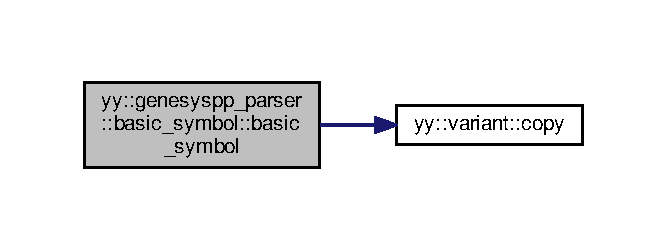
\includegraphics[width=320pt]{structyy_1_1genesyspp__parser_1_1basic__symbol_a94529fa808d843d97fad2b531bd04466_cgraph}
\end{center}
\end{figure}


\hypertarget{structyy_1_1genesyspp__parser_1_1basic__symbol_aeaa054339c41c834ec30bbda4dc3beff}{\index{yy\-::genesyspp\-\_\-parser\-::basic\-\_\-symbol@{yy\-::genesyspp\-\_\-parser\-::basic\-\_\-symbol}!$\sim$basic\-\_\-symbol@{$\sim$basic\-\_\-symbol}}
\index{$\sim$basic\-\_\-symbol@{$\sim$basic\-\_\-symbol}!yy::genesyspp_parser::basic_symbol@{yy\-::genesyspp\-\_\-parser\-::basic\-\_\-symbol}}
\subsubsection[{$\sim$basic\-\_\-symbol}]{\setlength{\rightskip}{0pt plus 5cm}template$<$typename Base $>$ {\bf yy\-::genesyspp\-\_\-parser\-::basic\-\_\-symbol}$<$ Base $>$\-::$\sim${\bf basic\-\_\-symbol} (
\begin{DoxyParamCaption}
{}
\end{DoxyParamCaption}
)}}\label{structyy_1_1genesyspp__parser_1_1basic__symbol_aeaa054339c41c834ec30bbda4dc3beff}


Destroy the symbol. 



Definition at line 1270 of file Genesys++-\/parser.\-h.



\subsection{Member Function Documentation}
\hypertarget{structyy_1_1genesyspp__parser_1_1basic__symbol_a307cece0deecd34ac5f4812a92d69d0b}{\index{yy\-::genesyspp\-\_\-parser\-::basic\-\_\-symbol@{yy\-::genesyspp\-\_\-parser\-::basic\-\_\-symbol}!clear@{clear}}
\index{clear@{clear}!yy::genesyspp_parser::basic_symbol@{yy\-::genesyspp\-\_\-parser\-::basic\-\_\-symbol}}
\subsubsection[{clear}]{\setlength{\rightskip}{0pt plus 5cm}template$<$typename Base $>$ void {\bf yy\-::genesyspp\-\_\-parser\-::basic\-\_\-symbol}$<$ Base $>$\-::clear (
\begin{DoxyParamCaption}
{}
\end{DoxyParamCaption}
)}}\label{structyy_1_1genesyspp__parser_1_1basic__symbol_a307cece0deecd34ac5f4812a92d69d0b}


Destroy contents, and record that is empty. 



Definition at line 1277 of file Genesys++-\/parser.\-h.



Here is the caller graph for this function\-:
\nopagebreak
\begin{figure}[H]
\begin{center}
\leavevmode
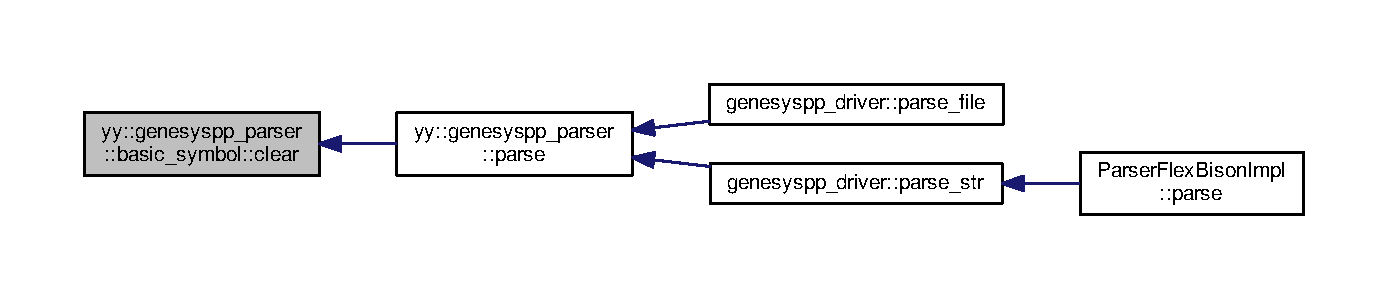
\includegraphics[width=350pt]{structyy_1_1genesyspp__parser_1_1basic__symbol_a307cece0deecd34ac5f4812a92d69d0b_icgraph}
\end{center}
\end{figure}


\hypertarget{structyy_1_1genesyspp__parser_1_1basic__symbol_af31a4325622f49b9903cdc6734e4f9d8}{\index{yy\-::genesyspp\-\_\-parser\-::basic\-\_\-symbol@{yy\-::genesyspp\-\_\-parser\-::basic\-\_\-symbol}!empty@{empty}}
\index{empty@{empty}!yy::genesyspp_parser::basic_symbol@{yy\-::genesyspp\-\_\-parser\-::basic\-\_\-symbol}}
\subsubsection[{empty}]{\setlength{\rightskip}{0pt plus 5cm}template$<$typename Base $>$ bool {\bf yy\-::genesyspp\-\_\-parser\-::basic\-\_\-symbol}$<$ Base $>$\-::empty (
\begin{DoxyParamCaption}
{}
\end{DoxyParamCaption}
) const}}\label{structyy_1_1genesyspp__parser_1_1basic__symbol_af31a4325622f49b9903cdc6734e4f9d8}


Whether empty. 



Definition at line 1372 of file Genesys++-\/parser.\-h.



Here is the caller graph for this function\-:
\nopagebreak
\begin{figure}[H]
\begin{center}
\leavevmode
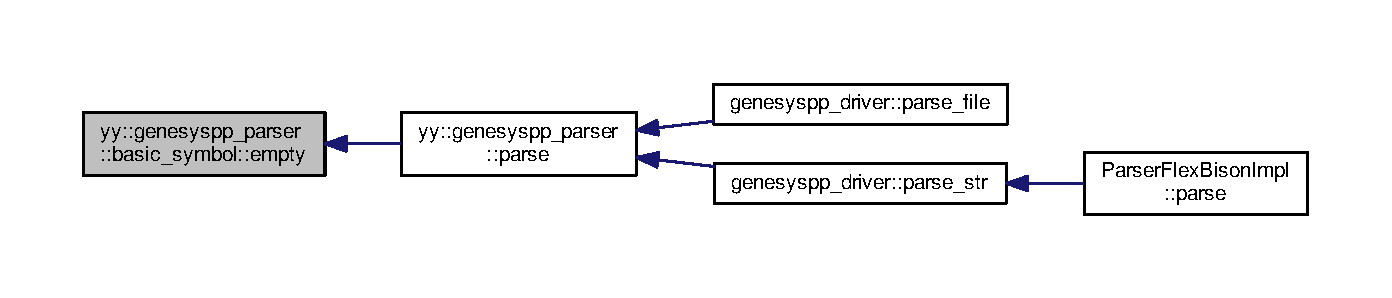
\includegraphics[width=350pt]{structyy_1_1genesyspp__parser_1_1basic__symbol_af31a4325622f49b9903cdc6734e4f9d8_icgraph}
\end{center}
\end{figure}


\hypertarget{structyy_1_1genesyspp__parser_1_1basic__symbol_a4244f8c6794d7869a9e82a96cd49e5f2}{\index{yy\-::genesyspp\-\_\-parser\-::basic\-\_\-symbol@{yy\-::genesyspp\-\_\-parser\-::basic\-\_\-symbol}!move@{move}}
\index{move@{move}!yy::genesyspp_parser::basic_symbol@{yy\-::genesyspp\-\_\-parser\-::basic\-\_\-symbol}}
\subsubsection[{move}]{\setlength{\rightskip}{0pt plus 5cm}template$<$typename Base $>$ void {\bf yy\-::genesyspp\-\_\-parser\-::basic\-\_\-symbol}$<$ Base $>$\-::move (
\begin{DoxyParamCaption}
\item[{{\bf basic\-\_\-symbol}$<$ Base $>$ \&}]{s}
\end{DoxyParamCaption}
)}}\label{structyy_1_1genesyspp__parser_1_1basic__symbol_a4244f8c6794d7869a9e82a96cd49e5f2}


Destructive move, {\itshape s} is emptied into this. 



Definition at line 1379 of file Genesys++-\/parser.\-h.



Here is the caller graph for this function\-:
\nopagebreak
\begin{figure}[H]
\begin{center}
\leavevmode
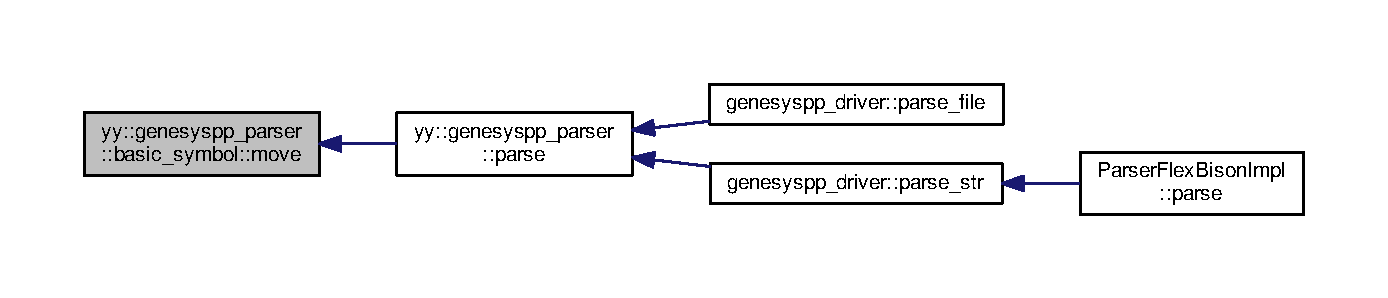
\includegraphics[width=350pt]{structyy_1_1genesyspp__parser_1_1basic__symbol_a4244f8c6794d7869a9e82a96cd49e5f2_icgraph}
\end{center}
\end{figure}




\subsection{Member Data Documentation}
\hypertarget{structyy_1_1genesyspp__parser_1_1basic__symbol_ae95666bbb377d80e31b8a676aa44e84a}{\index{yy\-::genesyspp\-\_\-parser\-::basic\-\_\-symbol@{yy\-::genesyspp\-\_\-parser\-::basic\-\_\-symbol}!location@{location}}
\index{location@{location}!yy::genesyspp_parser::basic_symbol@{yy\-::genesyspp\-\_\-parser\-::basic\-\_\-symbol}}
\subsubsection[{location}]{\setlength{\rightskip}{0pt plus 5cm}template$<$typename Base$>$ {\bf location\-\_\-type} {\bf yy\-::genesyspp\-\_\-parser\-::basic\-\_\-symbol}$<$ Base $>$\-::{\bf location}}}\label{structyy_1_1genesyspp__parser_1_1basic__symbol_ae95666bbb377d80e31b8a676aa44e84a}


The location. 



Definition at line 519 of file Genesys++-\/parser.\-h.

\hypertarget{structyy_1_1genesyspp__parser_1_1basic__symbol_a66fa4a750b9ae7e8be9c640b8712fe0b}{\index{yy\-::genesyspp\-\_\-parser\-::basic\-\_\-symbol@{yy\-::genesyspp\-\_\-parser\-::basic\-\_\-symbol}!value@{value}}
\index{value@{value}!yy::genesyspp_parser::basic_symbol@{yy\-::genesyspp\-\_\-parser\-::basic\-\_\-symbol}}
\subsubsection[{value}]{\setlength{\rightskip}{0pt plus 5cm}template$<$typename Base$>$ {\bf semantic\-\_\-type} {\bf yy\-::genesyspp\-\_\-parser\-::basic\-\_\-symbol}$<$ Base $>$\-::value}}\label{structyy_1_1genesyspp__parser_1_1basic__symbol_a66fa4a750b9ae7e8be9c640b8712fe0b}


The semantic value. 



Definition at line 516 of file Genesys++-\/parser.\-h.



The documentation for this struct was generated from the following file\-:\begin{DoxyCompactItemize}
\item 
\hyperlink{_genesys_09_09-parser_8h}{Genesys++-\/parser.\-h}\end{DoxyCompactItemize}

\hypertarget{class_build_simulation_model}{\section{Build\-Simulation\-Model Class Reference}
\label{class_build_simulation_model}\index{Build\-Simulation\-Model@{Build\-Simulation\-Model}}
}


{\ttfamily \#include $<$Build\-Simulation\-Model.\-h$>$}



Inheritance diagram for Build\-Simulation\-Model\-:
\nopagebreak
\begin{figure}[H]
\begin{center}
\leavevmode
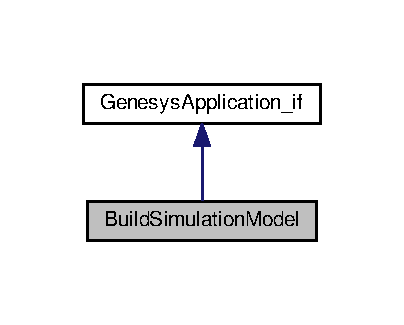
\includegraphics[width=194pt]{class_build_simulation_model__inherit__graph}
\end{center}
\end{figure}


Collaboration diagram for Build\-Simulation\-Model\-:
\nopagebreak
\begin{figure}[H]
\begin{center}
\leavevmode
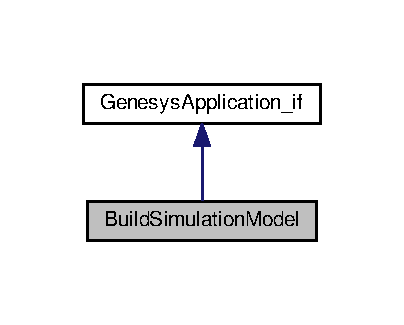
\includegraphics[width=194pt]{class_build_simulation_model__coll__graph}
\end{center}
\end{figure}
\subsection*{Public Member Functions}
\begin{DoxyCompactItemize}
\item 
\hyperlink{class_build_simulation_model_a477872592a89845e00cfbc7b6063bb21}{Build\-Simulation\-Model} ()
\item 
int \hyperlink{class_build_simulation_model_a8c50f55d7293860e5e7bc7e7e74f8d4a}{main} (int argc, char $\ast$$\ast$argv)
\end{DoxyCompactItemize}


\subsection{Detailed Description}


Definition at line 19 of file Build\-Simulation\-Model.\-h.



\subsection{Constructor \& Destructor Documentation}
\hypertarget{class_build_simulation_model_a477872592a89845e00cfbc7b6063bb21}{\index{Build\-Simulation\-Model@{Build\-Simulation\-Model}!Build\-Simulation\-Model@{Build\-Simulation\-Model}}
\index{Build\-Simulation\-Model@{Build\-Simulation\-Model}!BuildSimulationModel@{Build\-Simulation\-Model}}
\subsubsection[{Build\-Simulation\-Model}]{\setlength{\rightskip}{0pt plus 5cm}Build\-Simulation\-Model\-::\-Build\-Simulation\-Model (
\begin{DoxyParamCaption}
{}
\end{DoxyParamCaption}
)}}\label{class_build_simulation_model_a477872592a89845e00cfbc7b6063bb21}


Definition at line 102 of file Build\-Simulation\-Model.\-cpp.



\subsection{Member Function Documentation}
\hypertarget{class_build_simulation_model_a8c50f55d7293860e5e7bc7e7e74f8d4a}{\index{Build\-Simulation\-Model@{Build\-Simulation\-Model}!main@{main}}
\index{main@{main}!BuildSimulationModel@{Build\-Simulation\-Model}}
\subsubsection[{main}]{\setlength{\rightskip}{0pt plus 5cm}int Build\-Simulation\-Model\-::main (
\begin{DoxyParamCaption}
\item[{int}]{argc, }
\item[{char $\ast$$\ast$}]{argv}
\end{DoxyParamCaption}
)\hspace{0.3cm}{\ttfamily [virtual]}}}\label{class_build_simulation_model_a8c50f55d7293860e5e7bc7e7e74f8d4a}


Implements \hyperlink{class_genesys_application__if_a2b07e7803b410a4a8d0f87422dabb004}{Genesys\-Application\-\_\-if}.



Definition at line 117 of file Build\-Simulation\-Model.\-cpp.



Here is the call graph for this function\-:
\nopagebreak
\begin{figure}[H]
\begin{center}
\leavevmode
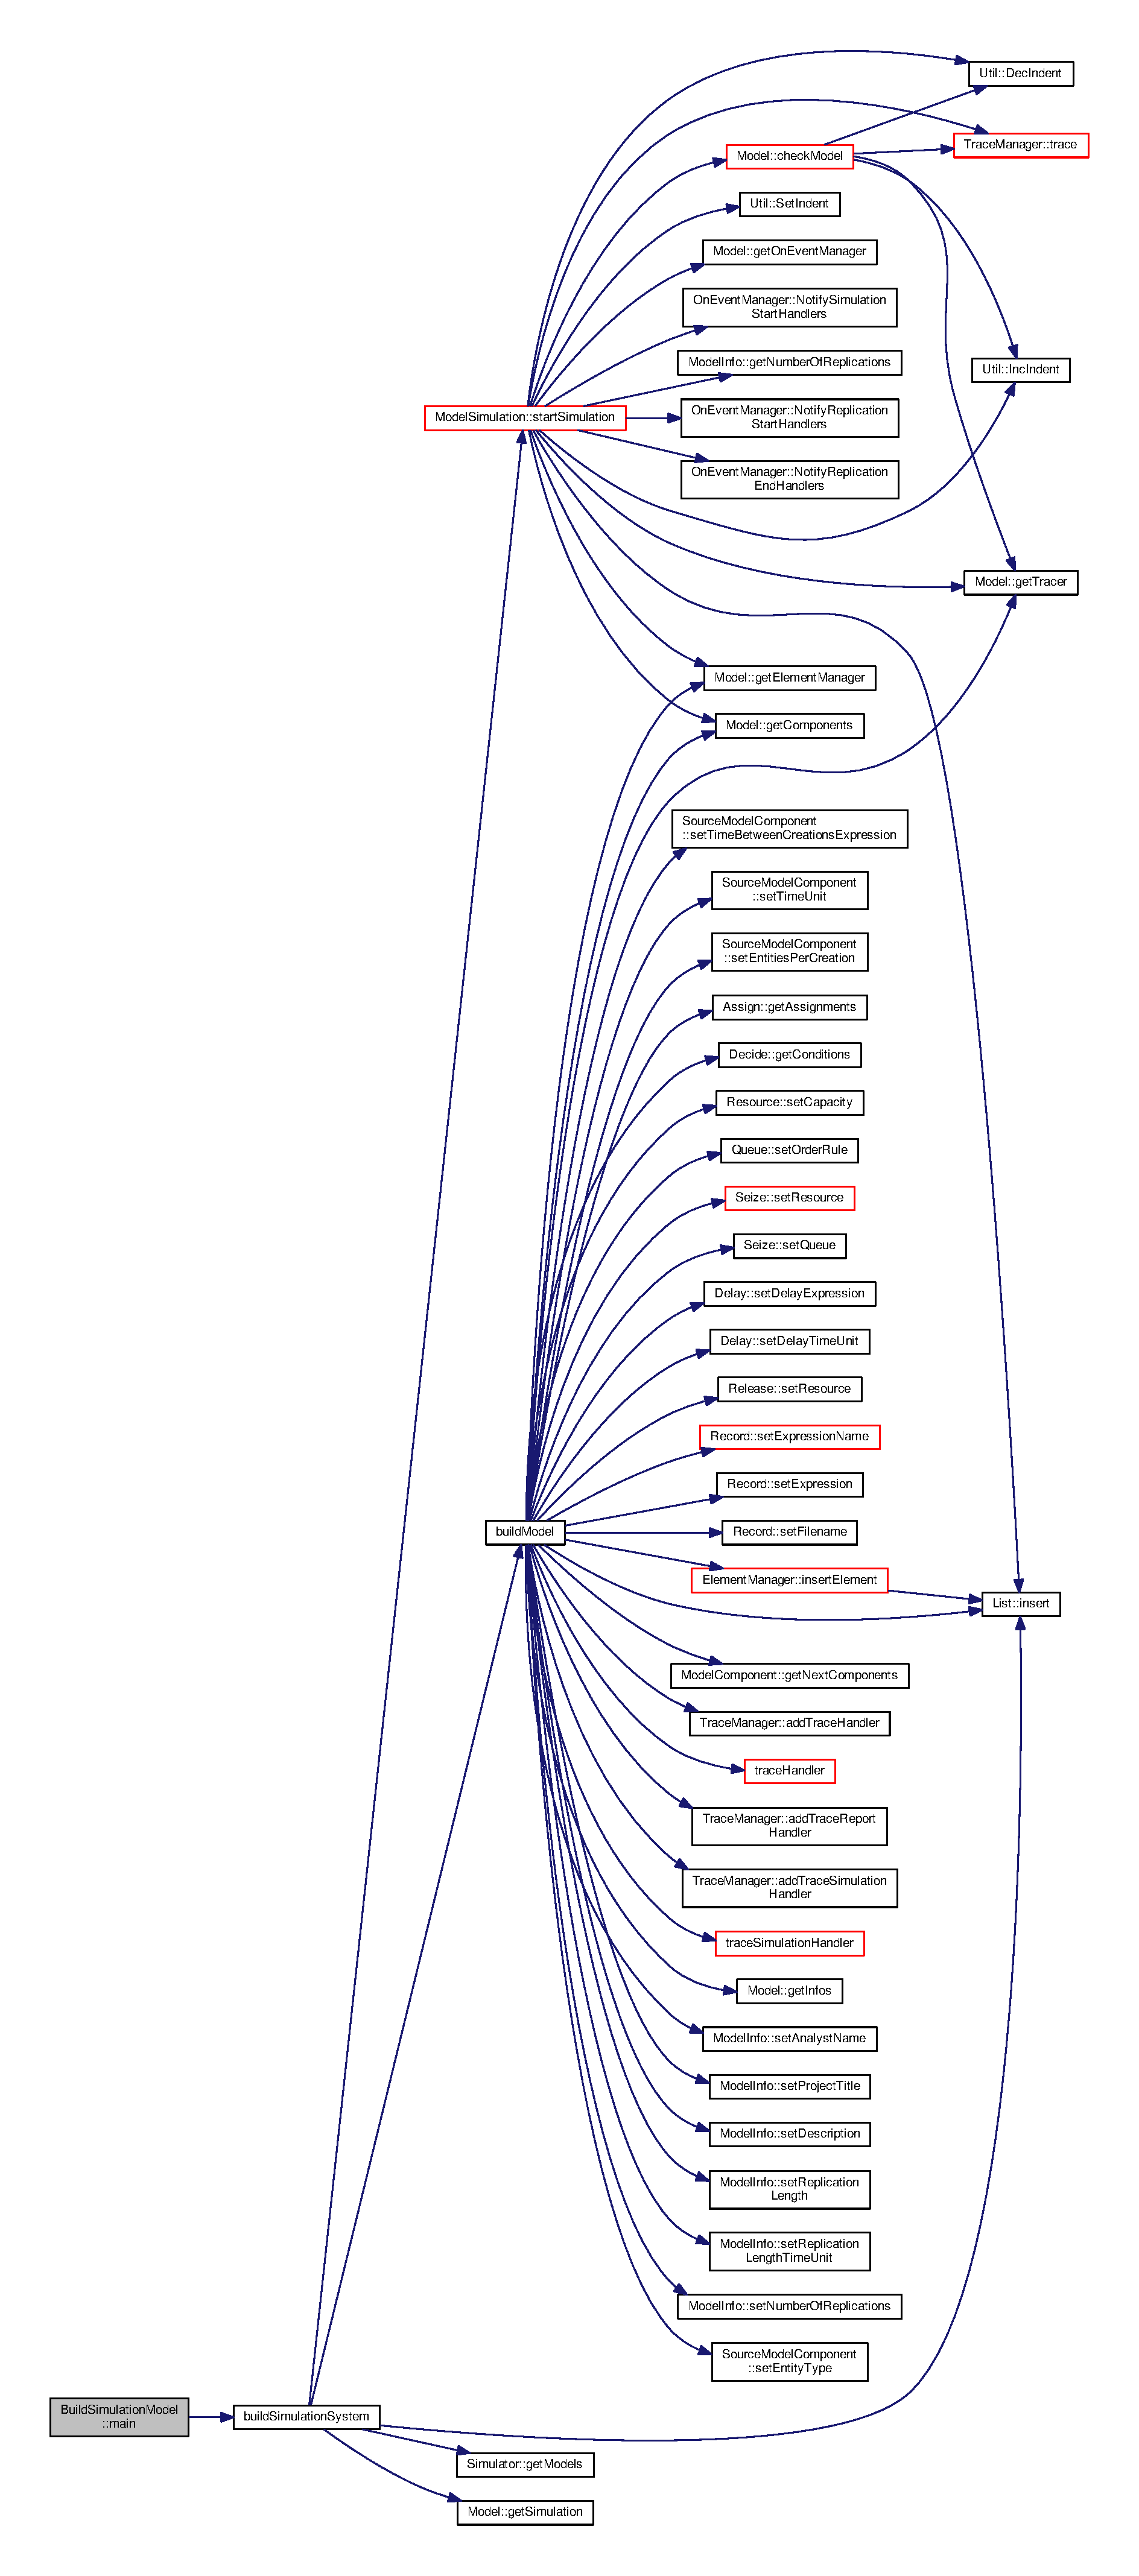
\includegraphics[height=550pt]{class_build_simulation_model_a8c50f55d7293860e5e7bc7e7e74f8d4a_cgraph}
\end{center}
\end{figure}




The documentation for this class was generated from the following files\-:\begin{DoxyCompactItemize}
\item 
\hyperlink{_build_simulation_model_8h}{Build\-Simulation\-Model.\-h}\item 
\hyperlink{_build_simulation_model_8cpp}{Build\-Simulation\-Model.\-cpp}\end{DoxyCompactItemize}

\hypertarget{structyy_1_1genesyspp__parser_1_1by__type}{\section{yy\-:\-:genesyspp\-\_\-parser\-:\-:by\-\_\-type Struct Reference}
\label{structyy_1_1genesyspp__parser_1_1by__type}\index{yy\-::genesyspp\-\_\-parser\-::by\-\_\-type@{yy\-::genesyspp\-\_\-parser\-::by\-\_\-type}}
}


Type access provider for token (enum) based symbols.  




{\ttfamily \#include $<$Genesys++-\/parser.\-h$>$}

\subsection*{Public Types}
\begin{DoxyCompactItemize}
\item 
typedef \hyperlink{structyy_1_1genesyspp__parser_1_1token_a473652e1e69da7c38a16e5d2aaac94b9}{token\-\_\-type} \hyperlink{structyy_1_1genesyspp__parser_1_1by__type_a7a616822e1a3b0a196ab34118104c384}{kind\-\_\-type}
\begin{DoxyCompactList}\small\item\em The symbol type as needed by the constructor. \end{DoxyCompactList}\end{DoxyCompactItemize}
\subsection*{Public Member Functions}
\begin{DoxyCompactItemize}
\item 
\hyperlink{structyy_1_1genesyspp__parser_1_1by__type_a76eabb9eead69b90ad4b430a345e88ef}{by\-\_\-type} ()
\begin{DoxyCompactList}\small\item\em Default constructor. \end{DoxyCompactList}\item 
\hyperlink{structyy_1_1genesyspp__parser_1_1by__type_a5392a679bcd401fe0243a69e7f422427}{by\-\_\-type} (const \hyperlink{structyy_1_1genesyspp__parser_1_1by__type}{by\-\_\-type} \&other)
\begin{DoxyCompactList}\small\item\em Copy constructor. \end{DoxyCompactList}\item 
\hyperlink{structyy_1_1genesyspp__parser_1_1by__type_af6af5f6a0a06e2fbb3b195bacf6f03d0}{by\-\_\-type} (\hyperlink{structyy_1_1genesyspp__parser_1_1token_a473652e1e69da7c38a16e5d2aaac94b9}{kind\-\_\-type} t)
\begin{DoxyCompactList}\small\item\em Constructor from (external) token numbers. \end{DoxyCompactList}\item 
void \hyperlink{structyy_1_1genesyspp__parser_1_1by__type_a8d4da60977a39a1d052686ee598bbbe8}{clear} ()
\begin{DoxyCompactList}\small\item\em Record that this symbol is empty. \end{DoxyCompactList}\item 
void \hyperlink{structyy_1_1genesyspp__parser_1_1by__type_a63b1bfb65f247edb690819fedd8ae756}{move} (\hyperlink{structyy_1_1genesyspp__parser_1_1by__type}{by\-\_\-type} \&that)
\begin{DoxyCompactList}\small\item\em Steal the symbol type from {\itshape that}. \end{DoxyCompactList}\item 
\hyperlink{classyy_1_1genesyspp__parser_a0910f625bff73225656c83490dd5fe9f}{symbol\-\_\-number\-\_\-type} \hyperlink{structyy_1_1genesyspp__parser_1_1by__type_ac56d30e24d923209a227d356e007e34c}{type\-\_\-get} () const 
\item 
\hyperlink{structyy_1_1genesyspp__parser_1_1token_a473652e1e69da7c38a16e5d2aaac94b9}{token\-\_\-type} \hyperlink{structyy_1_1genesyspp__parser_1_1by__type_a24ca814699206c1c9d29e22b1a4d6cfc}{token} () const 
\begin{DoxyCompactList}\small\item\em The token. \end{DoxyCompactList}\end{DoxyCompactItemize}
\subsection*{Public Attributes}
\begin{DoxyCompactItemize}
\item 
int \hyperlink{structyy_1_1genesyspp__parser_1_1by__type_a3ab3fb8851f9a2bc0b7703ad54b9bb19}{type}
\end{DoxyCompactItemize}


\subsection{Detailed Description}
Type access provider for token (enum) based symbols. 

Definition at line 527 of file Genesys++-\/parser.\-h.



\subsection{Member Typedef Documentation}
\hypertarget{structyy_1_1genesyspp__parser_1_1by__type_a7a616822e1a3b0a196ab34118104c384}{\index{yy\-::genesyspp\-\_\-parser\-::by\-\_\-type@{yy\-::genesyspp\-\_\-parser\-::by\-\_\-type}!kind\-\_\-type@{kind\-\_\-type}}
\index{kind\-\_\-type@{kind\-\_\-type}!yy::genesyspp_parser::by_type@{yy\-::genesyspp\-\_\-parser\-::by\-\_\-type}}
\subsubsection[{kind\-\_\-type}]{\setlength{\rightskip}{0pt plus 5cm}typedef {\bf token\-\_\-type} {\bf yy\-::genesyspp\-\_\-parser\-::by\-\_\-type\-::kind\-\_\-type}}}\label{structyy_1_1genesyspp__parser_1_1by__type_a7a616822e1a3b0a196ab34118104c384}


The symbol type as needed by the constructor. 



Definition at line 536 of file Genesys++-\/parser.\-h.



\subsection{Constructor \& Destructor Documentation}
\hypertarget{structyy_1_1genesyspp__parser_1_1by__type_a76eabb9eead69b90ad4b430a345e88ef}{\index{yy\-::genesyspp\-\_\-parser\-::by\-\_\-type@{yy\-::genesyspp\-\_\-parser\-::by\-\_\-type}!by\-\_\-type@{by\-\_\-type}}
\index{by\-\_\-type@{by\-\_\-type}!yy::genesyspp_parser::by_type@{yy\-::genesyspp\-\_\-parser\-::by\-\_\-type}}
\subsubsection[{by\-\_\-type}]{\setlength{\rightskip}{0pt plus 5cm}yy\-::genesyspp\-\_\-parser\-::by\-\_\-type\-::by\-\_\-type (
\begin{DoxyParamCaption}
{}
\end{DoxyParamCaption}
)\hspace{0.3cm}{\ttfamily [inline]}}}\label{structyy_1_1genesyspp__parser_1_1by__type_a76eabb9eead69b90ad4b430a345e88ef}


Default constructor. 



Definition at line 1464 of file Genesys++-\/parser.\-h.

\hypertarget{structyy_1_1genesyspp__parser_1_1by__type_a5392a679bcd401fe0243a69e7f422427}{\index{yy\-::genesyspp\-\_\-parser\-::by\-\_\-type@{yy\-::genesyspp\-\_\-parser\-::by\-\_\-type}!by\-\_\-type@{by\-\_\-type}}
\index{by\-\_\-type@{by\-\_\-type}!yy::genesyspp_parser::by_type@{yy\-::genesyspp\-\_\-parser\-::by\-\_\-type}}
\subsubsection[{by\-\_\-type}]{\setlength{\rightskip}{0pt plus 5cm}yy\-::genesyspp\-\_\-parser\-::by\-\_\-type\-::by\-\_\-type (
\begin{DoxyParamCaption}
\item[{const {\bf by\-\_\-type} \&}]{other}
\end{DoxyParamCaption}
)\hspace{0.3cm}{\ttfamily [inline]}}}\label{structyy_1_1genesyspp__parser_1_1by__type_a5392a679bcd401fe0243a69e7f422427}


Copy constructor. 



Definition at line 1469 of file Genesys++-\/parser.\-h.

\hypertarget{structyy_1_1genesyspp__parser_1_1by__type_af6af5f6a0a06e2fbb3b195bacf6f03d0}{\index{yy\-::genesyspp\-\_\-parser\-::by\-\_\-type@{yy\-::genesyspp\-\_\-parser\-::by\-\_\-type}!by\-\_\-type@{by\-\_\-type}}
\index{by\-\_\-type@{by\-\_\-type}!yy::genesyspp_parser::by_type@{yy\-::genesyspp\-\_\-parser\-::by\-\_\-type}}
\subsubsection[{by\-\_\-type}]{\setlength{\rightskip}{0pt plus 5cm}yy\-::genesyspp\-\_\-parser\-::by\-\_\-type\-::by\-\_\-type (
\begin{DoxyParamCaption}
\item[{{\bf kind\-\_\-type}}]{t}
\end{DoxyParamCaption}
)\hspace{0.3cm}{\ttfamily [inline]}}}\label{structyy_1_1genesyspp__parser_1_1by__type_af6af5f6a0a06e2fbb3b195bacf6f03d0}


Constructor from (external) token numbers. 



Definition at line 1474 of file Genesys++-\/parser.\-h.



\subsection{Member Function Documentation}
\hypertarget{structyy_1_1genesyspp__parser_1_1by__type_a8d4da60977a39a1d052686ee598bbbe8}{\index{yy\-::genesyspp\-\_\-parser\-::by\-\_\-type@{yy\-::genesyspp\-\_\-parser\-::by\-\_\-type}!clear@{clear}}
\index{clear@{clear}!yy::genesyspp_parser::by_type@{yy\-::genesyspp\-\_\-parser\-::by\-\_\-type}}
\subsubsection[{clear}]{\setlength{\rightskip}{0pt plus 5cm}void yy\-::genesyspp\-\_\-parser\-::by\-\_\-type\-::clear (
\begin{DoxyParamCaption}
{}
\end{DoxyParamCaption}
)\hspace{0.3cm}{\ttfamily [inline]}}}\label{structyy_1_1genesyspp__parser_1_1by__type_a8d4da60977a39a1d052686ee598bbbe8}


Record that this symbol is empty. 



Definition at line 1480 of file Genesys++-\/parser.\-h.



Here is the caller graph for this function\-:\nopagebreak
\begin{figure}[H]
\begin{center}
\leavevmode
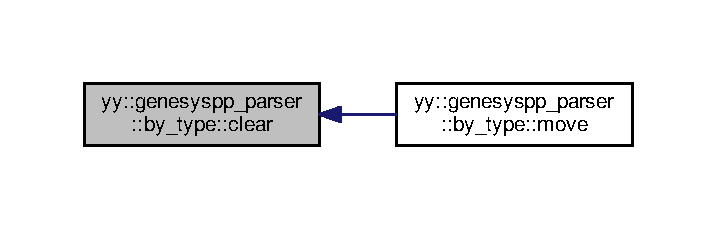
\includegraphics[width=344pt]{structyy_1_1genesyspp__parser_1_1by__type_a8d4da60977a39a1d052686ee598bbbe8_icgraph}
\end{center}
\end{figure}


\hypertarget{structyy_1_1genesyspp__parser_1_1by__type_a63b1bfb65f247edb690819fedd8ae756}{\index{yy\-::genesyspp\-\_\-parser\-::by\-\_\-type@{yy\-::genesyspp\-\_\-parser\-::by\-\_\-type}!move@{move}}
\index{move@{move}!yy::genesyspp_parser::by_type@{yy\-::genesyspp\-\_\-parser\-::by\-\_\-type}}
\subsubsection[{move}]{\setlength{\rightskip}{0pt plus 5cm}void yy\-::genesyspp\-\_\-parser\-::by\-\_\-type\-::move (
\begin{DoxyParamCaption}
\item[{{\bf by\-\_\-type} \&}]{that}
\end{DoxyParamCaption}
)\hspace{0.3cm}{\ttfamily [inline]}}}\label{structyy_1_1genesyspp__parser_1_1by__type_a63b1bfb65f247edb690819fedd8ae756}


Steal the symbol type from {\itshape that}. 



Definition at line 1487 of file Genesys++-\/parser.\-h.



Here is the call graph for this function\-:\nopagebreak
\begin{figure}[H]
\begin{center}
\leavevmode
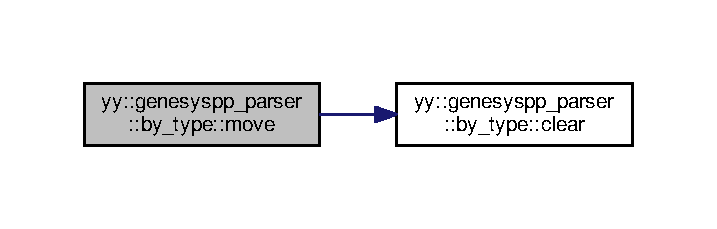
\includegraphics[width=344pt]{structyy_1_1genesyspp__parser_1_1by__type_a63b1bfb65f247edb690819fedd8ae756_cgraph}
\end{center}
\end{figure}


\hypertarget{structyy_1_1genesyspp__parser_1_1by__type_a24ca814699206c1c9d29e22b1a4d6cfc}{\index{yy\-::genesyspp\-\_\-parser\-::by\-\_\-type@{yy\-::genesyspp\-\_\-parser\-::by\-\_\-type}!token@{token}}
\index{token@{token}!yy::genesyspp_parser::by_type@{yy\-::genesyspp\-\_\-parser\-::by\-\_\-type}}
\subsubsection[{token}]{\setlength{\rightskip}{0pt plus 5cm}{\bf genesyspp\-\_\-parser\-::token\-\_\-type} yy\-::genesyspp\-\_\-parser\-::by\-\_\-type\-::token (
\begin{DoxyParamCaption}
{}
\end{DoxyParamCaption}
) const\hspace{0.3cm}{\ttfamily [inline]}}}\label{structyy_1_1genesyspp__parser_1_1by__type_a24ca814699206c1c9d29e22b1a4d6cfc}


The token. 



Definition at line 1502 of file Genesys++-\/parser.\-h.

\hypertarget{structyy_1_1genesyspp__parser_1_1by__type_ac56d30e24d923209a227d356e007e34c}{\index{yy\-::genesyspp\-\_\-parser\-::by\-\_\-type@{yy\-::genesyspp\-\_\-parser\-::by\-\_\-type}!type\-\_\-get@{type\-\_\-get}}
\index{type\-\_\-get@{type\-\_\-get}!yy::genesyspp_parser::by_type@{yy\-::genesyspp\-\_\-parser\-::by\-\_\-type}}
\subsubsection[{type\-\_\-get}]{\setlength{\rightskip}{0pt plus 5cm}int yy\-::genesyspp\-\_\-parser\-::by\-\_\-type\-::type\-\_\-get (
\begin{DoxyParamCaption}
{}
\end{DoxyParamCaption}
) const\hspace{0.3cm}{\ttfamily [inline]}}}\label{structyy_1_1genesyspp__parser_1_1by__type_ac56d30e24d923209a227d356e007e34c}
The (internal) type number (corresponding to {\itshape type}). {\itshape empty} when empty. 

Definition at line 1495 of file Genesys++-\/parser.\-h.



\subsection{Member Data Documentation}
\hypertarget{structyy_1_1genesyspp__parser_1_1by__type_a3ab3fb8851f9a2bc0b7703ad54b9bb19}{\index{yy\-::genesyspp\-\_\-parser\-::by\-\_\-type@{yy\-::genesyspp\-\_\-parser\-::by\-\_\-type}!type@{type}}
\index{type@{type}!yy::genesyspp_parser::by_type@{yy\-::genesyspp\-\_\-parser\-::by\-\_\-type}}
\subsubsection[{type}]{\setlength{\rightskip}{0pt plus 5cm}int yy\-::genesyspp\-\_\-parser\-::by\-\_\-type\-::type}}\label{structyy_1_1genesyspp__parser_1_1by__type_a3ab3fb8851f9a2bc0b7703ad54b9bb19}
The symbol type. {\itshape empty\-\_\-symbol} when empty. An int, not token\-\_\-number\-\_\-type, to be able to store empty\-\_\-symbol. 

Definition at line 557 of file Genesys++-\/parser.\-h.



The documentation for this struct was generated from the following file\-:\begin{DoxyCompactItemize}
\item 
\hyperlink{_genesys_09_09-parser_8h}{Genesys++-\/parser.\-h}\end{DoxyCompactItemize}

\hypertarget{class_collector__if}{\section{Collector\-\_\-if Class Reference}
\label{class_collector__if}\index{Collector\-\_\-if@{Collector\-\_\-if}}
}


{\ttfamily \#include $<$Collector\-\_\-if.\-h$>$}



Inheritance diagram for Collector\-\_\-if\-:\nopagebreak
\begin{figure}[H]
\begin{center}
\leavevmode
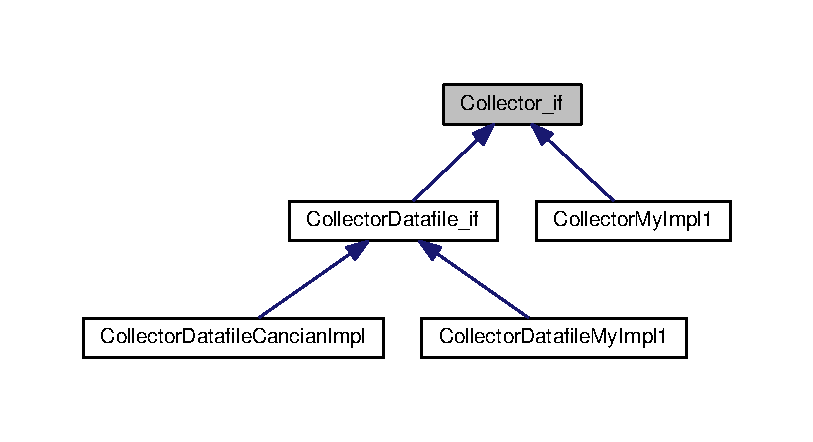
\includegraphics[width=350pt]{class_collector__if__inherit__graph}
\end{center}
\end{figure}
\subsection*{Public Member Functions}
\begin{DoxyCompactItemize}
\item 
virtual void \hyperlink{class_collector__if_a035bd1300c85866870c2f6178a9528e8}{clear} ()=0
\item 
virtual void \hyperlink{class_collector__if_ac7b83bce8ddb4903d247c1eddd656171}{add\-Value} (double value)=0
\item 
virtual double \hyperlink{class_collector__if_aa14f7e1065af8fd38ab592e224fb7e43}{get\-Last\-Value} ()=0
\item 
virtual unsigned long \hyperlink{class_collector__if_a97fa632508ffdfad1365b3a949acf745}{num\-Elements} ()=0
\end{DoxyCompactItemize}


\subsection{Detailed Description}
Interface for collecting values of a single stochastic variable. Values collected can be used as base for statistical analysis. 

Definition at line 22 of file Collector\-\_\-if.\-h.



\subsection{Member Function Documentation}
\hypertarget{class_collector__if_ac7b83bce8ddb4903d247c1eddd656171}{\index{Collector\-\_\-if@{Collector\-\_\-if}!add\-Value@{add\-Value}}
\index{add\-Value@{add\-Value}!Collector_if@{Collector\-\_\-if}}
\subsubsection[{add\-Value}]{\setlength{\rightskip}{0pt plus 5cm}virtual void Collector\-\_\-if\-::add\-Value (
\begin{DoxyParamCaption}
\item[{double}]{value}
\end{DoxyParamCaption}
)\hspace{0.3cm}{\ttfamily [pure virtual]}}}\label{class_collector__if_ac7b83bce8ddb4903d247c1eddd656171}


Implemented in \hyperlink{class_collector_datafile_cancian_impl_ab6a718100f5bdd04e3fef9edf23045ec}{Collector\-Datafile\-Cancian\-Impl}, \hyperlink{class_collector_my_impl1_acc5d658a3429af8b7d4265cbc37485b5}{Collector\-My\-Impl1}, and \hyperlink{class_collector_datafile_my_impl1_aa909fc87f2ee082512616840c9031365}{Collector\-Datafile\-My\-Impl1}.



Here is the caller graph for this function\-:\nopagebreak
\begin{figure}[H]
\begin{center}
\leavevmode
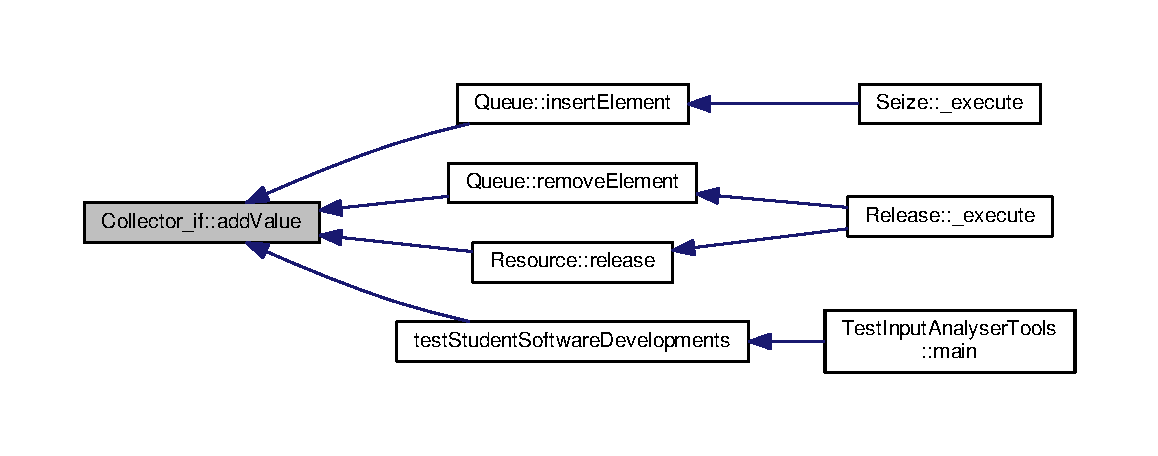
\includegraphics[width=350pt]{class_collector__if_ac7b83bce8ddb4903d247c1eddd656171_icgraph}
\end{center}
\end{figure}


\hypertarget{class_collector__if_a035bd1300c85866870c2f6178a9528e8}{\index{Collector\-\_\-if@{Collector\-\_\-if}!clear@{clear}}
\index{clear@{clear}!Collector_if@{Collector\-\_\-if}}
\subsubsection[{clear}]{\setlength{\rightskip}{0pt plus 5cm}virtual void Collector\-\_\-if\-::clear (
\begin{DoxyParamCaption}
{}
\end{DoxyParamCaption}
)\hspace{0.3cm}{\ttfamily [pure virtual]}}}\label{class_collector__if_a035bd1300c85866870c2f6178a9528e8}


Implemented in \hyperlink{class_collector_datafile_cancian_impl_a9fe0e4e764f1cc868d9c91bc68ff0ed8}{Collector\-Datafile\-Cancian\-Impl}, \hyperlink{class_collector_my_impl1_a9b570931955cafde878d6734aa914039}{Collector\-My\-Impl1}, and \hyperlink{class_collector_datafile_my_impl1_a594004f005db5dd1122946445f4db70d}{Collector\-Datafile\-My\-Impl1}.

\hypertarget{class_collector__if_aa14f7e1065af8fd38ab592e224fb7e43}{\index{Collector\-\_\-if@{Collector\-\_\-if}!get\-Last\-Value@{get\-Last\-Value}}
\index{get\-Last\-Value@{get\-Last\-Value}!Collector_if@{Collector\-\_\-if}}
\subsubsection[{get\-Last\-Value}]{\setlength{\rightskip}{0pt plus 5cm}virtual double Collector\-\_\-if\-::get\-Last\-Value (
\begin{DoxyParamCaption}
{}
\end{DoxyParamCaption}
)\hspace{0.3cm}{\ttfamily [pure virtual]}}}\label{class_collector__if_aa14f7e1065af8fd38ab592e224fb7e43}


Implemented in \hyperlink{class_collector_datafile_cancian_impl_a24b93dedb5f56e710e810c05e89dc36f}{Collector\-Datafile\-Cancian\-Impl}, \hyperlink{class_collector_my_impl1_a56e754ba3175e2f335290e2a737e7104}{Collector\-My\-Impl1}, and \hyperlink{class_collector_datafile_my_impl1_a5a29b2f71a4630c658fb83c047fb1054}{Collector\-Datafile\-My\-Impl1}.

\hypertarget{class_collector__if_a97fa632508ffdfad1365b3a949acf745}{\index{Collector\-\_\-if@{Collector\-\_\-if}!num\-Elements@{num\-Elements}}
\index{num\-Elements@{num\-Elements}!Collector_if@{Collector\-\_\-if}}
\subsubsection[{num\-Elements}]{\setlength{\rightskip}{0pt plus 5cm}virtual unsigned long Collector\-\_\-if\-::num\-Elements (
\begin{DoxyParamCaption}
{}
\end{DoxyParamCaption}
)\hspace{0.3cm}{\ttfamily [pure virtual]}}}\label{class_collector__if_a97fa632508ffdfad1365b3a949acf745}


Implemented in \hyperlink{class_collector_datafile_cancian_impl_ab10e682e4b991a881efb56caebb4efa9}{Collector\-Datafile\-Cancian\-Impl}, \hyperlink{class_collector_my_impl1_a25427d84682943e0f588d494c54f79d8}{Collector\-My\-Impl1}, and \hyperlink{class_collector_datafile_my_impl1_ac8ad59a3b664d082c8ca4fca9887148a}{Collector\-Datafile\-My\-Impl1}.



The documentation for this class was generated from the following file\-:\begin{DoxyCompactItemize}
\item 
\hyperlink{_collector__if_8h}{Collector\-\_\-if.\-h}\end{DoxyCompactItemize}

\hypertarget{class_collector_datafile__if}{\section{Collector\-Datafile\-\_\-if Class Reference}
\label{class_collector_datafile__if}\index{Collector\-Datafile\-\_\-if@{Collector\-Datafile\-\_\-if}}
}


{\ttfamily \#include $<$Collector\-Datafile\-\_\-if.\-h$>$}



Inheritance diagram for Collector\-Datafile\-\_\-if\-:
\nopagebreak
\begin{figure}[H]
\begin{center}
\leavevmode
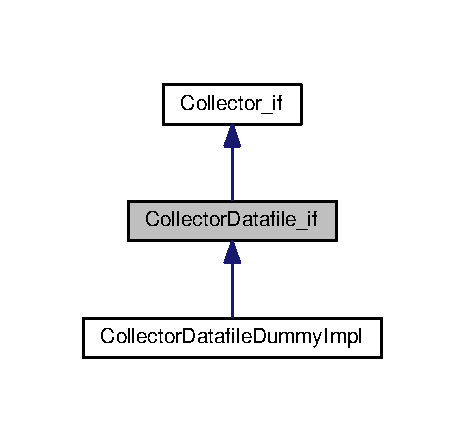
\includegraphics[width=206pt]{class_collector_datafile__if__inherit__graph}
\end{center}
\end{figure}


Collaboration diagram for Collector\-Datafile\-\_\-if\-:
\nopagebreak
\begin{figure}[H]
\begin{center}
\leavevmode
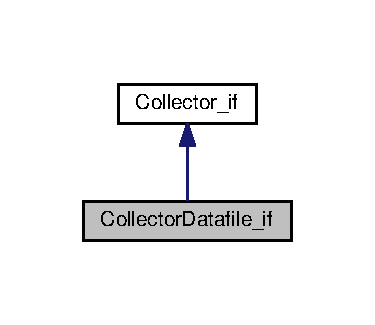
\includegraphics[width=180pt]{class_collector_datafile__if__coll__graph}
\end{center}
\end{figure}
\subsection*{Public Member Functions}
\begin{DoxyCompactItemize}
\item 
virtual double \hyperlink{class_collector_datafile__if_aa790efe68dfa16cebd66b481bbda8411}{get\-Value} (unsigned int num)=0
\item 
virtual std\-::string \hyperlink{class_collector_datafile__if_a81d109f34c25f5295f76ba13f4234a3c}{get\-Data\-Filename} ()=0
\item 
virtual void \hyperlink{class_collector_datafile__if_ab826bbf5472a5cfdbf2f2c30273da8eb}{set\-Data\-Filename} (std\-::string filename)=0
\end{DoxyCompactItemize}


\subsection{Member Function Documentation}
\hypertarget{class_collector_datafile__if_a81d109f34c25f5295f76ba13f4234a3c}{\index{Collector\-Datafile\-\_\-if@{Collector\-Datafile\-\_\-if}!get\-Data\-Filename@{get\-Data\-Filename}}
\index{get\-Data\-Filename@{get\-Data\-Filename}!CollectorDatafile_if@{Collector\-Datafile\-\_\-if}}
\subsubsection[{get\-Data\-Filename}]{\setlength{\rightskip}{0pt plus 5cm}virtual std\-::string Collector\-Datafile\-\_\-if\-::get\-Data\-Filename (
\begin{DoxyParamCaption}
{}
\end{DoxyParamCaption}
)\hspace{0.3cm}{\ttfamily [pure virtual]}}}\label{class_collector_datafile__if_a81d109f34c25f5295f76ba13f4234a3c}


Implemented in \hyperlink{class_collector_datafile_my_impl1_a5ebe8076b9eb9816a1b7d823943102cf}{Collector\-Datafile\-My\-Impl1}.

\hypertarget{class_collector_datafile__if_aa790efe68dfa16cebd66b481bbda8411}{\index{Collector\-Datafile\-\_\-if@{Collector\-Datafile\-\_\-if}!get\-Value@{get\-Value}}
\index{get\-Value@{get\-Value}!CollectorDatafile_if@{Collector\-Datafile\-\_\-if}}
\subsubsection[{get\-Value}]{\setlength{\rightskip}{0pt plus 5cm}virtual double Collector\-Datafile\-\_\-if\-::get\-Value (
\begin{DoxyParamCaption}
\item[{unsigned int}]{num}
\end{DoxyParamCaption}
)\hspace{0.3cm}{\ttfamily [pure virtual]}}}\label{class_collector_datafile__if_aa790efe68dfa16cebd66b481bbda8411}


Implemented in \hyperlink{class_collector_datafile_my_impl1_a55a505d56f9b95a55473bdf1ab24cffe}{Collector\-Datafile\-My\-Impl1}.

\hypertarget{class_collector_datafile__if_ab826bbf5472a5cfdbf2f2c30273da8eb}{\index{Collector\-Datafile\-\_\-if@{Collector\-Datafile\-\_\-if}!set\-Data\-Filename@{set\-Data\-Filename}}
\index{set\-Data\-Filename@{set\-Data\-Filename}!CollectorDatafile_if@{Collector\-Datafile\-\_\-if}}
\subsubsection[{set\-Data\-Filename}]{\setlength{\rightskip}{0pt plus 5cm}virtual void Collector\-Datafile\-\_\-if\-::set\-Data\-Filename (
\begin{DoxyParamCaption}
\item[{std\-::string}]{filename}
\end{DoxyParamCaption}
)\hspace{0.3cm}{\ttfamily [pure virtual]}}}\label{class_collector_datafile__if_ab826bbf5472a5cfdbf2f2c30273da8eb}


Implemented in \hyperlink{class_collector_datafile_my_impl1_ac4c401ae3cf4ccc723b6b9efa614ccd1}{Collector\-Datafile\-My\-Impl1}.



The documentation for this class was generated from the following file\-:\begin{DoxyCompactItemize}
\item 
\hyperlink{_collector_datafile__if_8h}{Collector\-Datafile\-\_\-if.\-h}\end{DoxyCompactItemize}

\hypertarget{class_collector_datafile_cancian_impl}{\section{Collector\-Datafile\-Cancian\-Impl Class Reference}
\label{class_collector_datafile_cancian_impl}\index{Collector\-Datafile\-Cancian\-Impl@{Collector\-Datafile\-Cancian\-Impl}}
}


{\ttfamily \#include $<$Collector\-Datafile\-Cancian\-Impl.\-h$>$}



Inheritance diagram for Collector\-Datafile\-Cancian\-Impl\-:\nopagebreak
\begin{figure}[H]
\begin{center}
\leavevmode
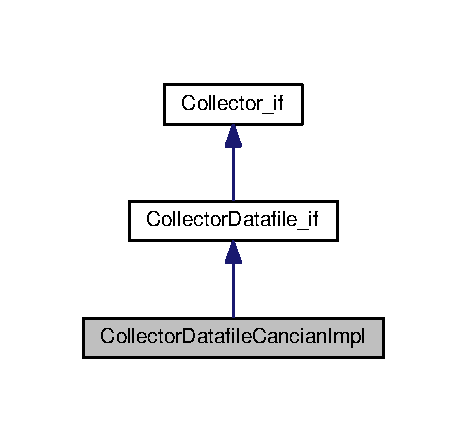
\includegraphics[width=224pt]{class_collector_datafile_cancian_impl__inherit__graph}
\end{center}
\end{figure}


Collaboration diagram for Collector\-Datafile\-Cancian\-Impl\-:\nopagebreak
\begin{figure}[H]
\begin{center}
\leavevmode
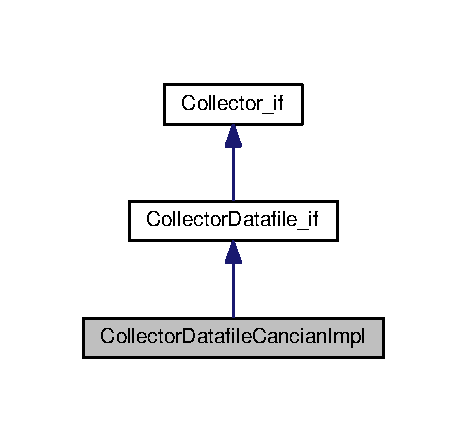
\includegraphics[width=224pt]{class_collector_datafile_cancian_impl__coll__graph}
\end{center}
\end{figure}
\subsection*{Public Member Functions}
\begin{DoxyCompactItemize}
\item 
\hyperlink{class_collector_datafile_cancian_impl_a7754e99ffee4aacf1538c26376ab6e00}{Collector\-Datafile\-Cancian\-Impl} ()
\item 
\hyperlink{class_collector_datafile_cancian_impl_ae69bb092854c71eb188d2df45487cdb4}{Collector\-Datafile\-Cancian\-Impl} (const \hyperlink{class_collector_datafile_cancian_impl}{Collector\-Datafile\-Cancian\-Impl} \&orig)
\item 
\hyperlink{class_collector_datafile_cancian_impl_a1c7a005af545e3d78f34e84350c199bf}{$\sim$\-Collector\-Datafile\-Cancian\-Impl} ()
\item 
void \hyperlink{class_collector_datafile_cancian_impl_a9fe0e4e764f1cc868d9c91bc68ff0ed8}{clear} ()
\item 
void \hyperlink{class_collector_datafile_cancian_impl_ab6a718100f5bdd04e3fef9edf23045ec}{add\-Value} (double value)
\item 
double \hyperlink{class_collector_datafile_cancian_impl_a24b93dedb5f56e710e810c05e89dc36f}{get\-Last\-Value} ()
\item 
unsigned long \hyperlink{class_collector_datafile_cancian_impl_ab10e682e4b991a881efb56caebb4efa9}{num\-Elements} ()
\item 
double \hyperlink{class_collector_datafile_cancian_impl_af06ad080b3b03269da8feff74a101670}{get\-Value} (unsigned int num)
\item 
std\-::string \hyperlink{class_collector_datafile_cancian_impl_a216e46f526becc3dd4b4772e07256b81}{get\-Data\-Filename} ()
\item 
void \hyperlink{class_collector_datafile_cancian_impl_a7fb058367bd603743d3636c39c44ca56}{set\-Data\-Filename} (std\-::string filename)
\end{DoxyCompactItemize}


\subsection{Detailed Description}


Definition at line 20 of file Collector\-Datafile\-Cancian\-Impl.\-h.



\subsection{Constructor \& Destructor Documentation}
\hypertarget{class_collector_datafile_cancian_impl_a7754e99ffee4aacf1538c26376ab6e00}{\index{Collector\-Datafile\-Cancian\-Impl@{Collector\-Datafile\-Cancian\-Impl}!Collector\-Datafile\-Cancian\-Impl@{Collector\-Datafile\-Cancian\-Impl}}
\index{Collector\-Datafile\-Cancian\-Impl@{Collector\-Datafile\-Cancian\-Impl}!CollectorDatafileCancianImpl@{Collector\-Datafile\-Cancian\-Impl}}
\subsubsection[{Collector\-Datafile\-Cancian\-Impl}]{\setlength{\rightskip}{0pt plus 5cm}Collector\-Datafile\-Cancian\-Impl\-::\-Collector\-Datafile\-Cancian\-Impl (
\begin{DoxyParamCaption}
{}
\end{DoxyParamCaption}
)}}\label{class_collector_datafile_cancian_impl_a7754e99ffee4aacf1538c26376ab6e00}


Definition at line 18 of file Collector\-Datafile\-Cancian\-Impl.\-cpp.

\hypertarget{class_collector_datafile_cancian_impl_ae69bb092854c71eb188d2df45487cdb4}{\index{Collector\-Datafile\-Cancian\-Impl@{Collector\-Datafile\-Cancian\-Impl}!Collector\-Datafile\-Cancian\-Impl@{Collector\-Datafile\-Cancian\-Impl}}
\index{Collector\-Datafile\-Cancian\-Impl@{Collector\-Datafile\-Cancian\-Impl}!CollectorDatafileCancianImpl@{Collector\-Datafile\-Cancian\-Impl}}
\subsubsection[{Collector\-Datafile\-Cancian\-Impl}]{\setlength{\rightskip}{0pt plus 5cm}Collector\-Datafile\-Cancian\-Impl\-::\-Collector\-Datafile\-Cancian\-Impl (
\begin{DoxyParamCaption}
\item[{const {\bf Collector\-Datafile\-Cancian\-Impl} \&}]{orig}
\end{DoxyParamCaption}
)}}\label{class_collector_datafile_cancian_impl_ae69bb092854c71eb188d2df45487cdb4}


Definition at line 21 of file Collector\-Datafile\-Cancian\-Impl.\-cpp.

\hypertarget{class_collector_datafile_cancian_impl_a1c7a005af545e3d78f34e84350c199bf}{\index{Collector\-Datafile\-Cancian\-Impl@{Collector\-Datafile\-Cancian\-Impl}!$\sim$\-Collector\-Datafile\-Cancian\-Impl@{$\sim$\-Collector\-Datafile\-Cancian\-Impl}}
\index{$\sim$\-Collector\-Datafile\-Cancian\-Impl@{$\sim$\-Collector\-Datafile\-Cancian\-Impl}!CollectorDatafileCancianImpl@{Collector\-Datafile\-Cancian\-Impl}}
\subsubsection[{$\sim$\-Collector\-Datafile\-Cancian\-Impl}]{\setlength{\rightskip}{0pt plus 5cm}Collector\-Datafile\-Cancian\-Impl\-::$\sim$\-Collector\-Datafile\-Cancian\-Impl (
\begin{DoxyParamCaption}
{}
\end{DoxyParamCaption}
)}}\label{class_collector_datafile_cancian_impl_a1c7a005af545e3d78f34e84350c199bf}


Definition at line 24 of file Collector\-Datafile\-Cancian\-Impl.\-cpp.



\subsection{Member Function Documentation}
\hypertarget{class_collector_datafile_cancian_impl_ab6a718100f5bdd04e3fef9edf23045ec}{\index{Collector\-Datafile\-Cancian\-Impl@{Collector\-Datafile\-Cancian\-Impl}!add\-Value@{add\-Value}}
\index{add\-Value@{add\-Value}!CollectorDatafileCancianImpl@{Collector\-Datafile\-Cancian\-Impl}}
\subsubsection[{add\-Value}]{\setlength{\rightskip}{0pt plus 5cm}void Collector\-Datafile\-Cancian\-Impl\-::add\-Value (
\begin{DoxyParamCaption}
\item[{double}]{value}
\end{DoxyParamCaption}
)\hspace{0.3cm}{\ttfamily [virtual]}}}\label{class_collector_datafile_cancian_impl_ab6a718100f5bdd04e3fef9edf23045ec}


Implements \hyperlink{class_collector__if_ac7b83bce8ddb4903d247c1eddd656171}{Collector\-\_\-if}.



Definition at line 33 of file Collector\-Datafile\-Cancian\-Impl.\-cpp.

\hypertarget{class_collector_datafile_cancian_impl_a9fe0e4e764f1cc868d9c91bc68ff0ed8}{\index{Collector\-Datafile\-Cancian\-Impl@{Collector\-Datafile\-Cancian\-Impl}!clear@{clear}}
\index{clear@{clear}!CollectorDatafileCancianImpl@{Collector\-Datafile\-Cancian\-Impl}}
\subsubsection[{clear}]{\setlength{\rightskip}{0pt plus 5cm}void Collector\-Datafile\-Cancian\-Impl\-::clear (
\begin{DoxyParamCaption}
{}
\end{DoxyParamCaption}
)\hspace{0.3cm}{\ttfamily [virtual]}}}\label{class_collector_datafile_cancian_impl_a9fe0e4e764f1cc868d9c91bc68ff0ed8}


Implements \hyperlink{class_collector__if_a035bd1300c85866870c2f6178a9528e8}{Collector\-\_\-if}.



Definition at line 27 of file Collector\-Datafile\-Cancian\-Impl.\-cpp.

\hypertarget{class_collector_datafile_cancian_impl_a216e46f526becc3dd4b4772e07256b81}{\index{Collector\-Datafile\-Cancian\-Impl@{Collector\-Datafile\-Cancian\-Impl}!get\-Data\-Filename@{get\-Data\-Filename}}
\index{get\-Data\-Filename@{get\-Data\-Filename}!CollectorDatafileCancianImpl@{Collector\-Datafile\-Cancian\-Impl}}
\subsubsection[{get\-Data\-Filename}]{\setlength{\rightskip}{0pt plus 5cm}std\-::string Collector\-Datafile\-Cancian\-Impl\-::get\-Data\-Filename (
\begin{DoxyParamCaption}
{}
\end{DoxyParamCaption}
)\hspace{0.3cm}{\ttfamily [virtual]}}}\label{class_collector_datafile_cancian_impl_a216e46f526becc3dd4b4772e07256b81}


Implements \hyperlink{class_collector_datafile__if_a81d109f34c25f5295f76ba13f4234a3c}{Collector\-Datafile\-\_\-if}.



Definition at line 70 of file Collector\-Datafile\-Cancian\-Impl.\-cpp.

\hypertarget{class_collector_datafile_cancian_impl_a24b93dedb5f56e710e810c05e89dc36f}{\index{Collector\-Datafile\-Cancian\-Impl@{Collector\-Datafile\-Cancian\-Impl}!get\-Last\-Value@{get\-Last\-Value}}
\index{get\-Last\-Value@{get\-Last\-Value}!CollectorDatafileCancianImpl@{Collector\-Datafile\-Cancian\-Impl}}
\subsubsection[{get\-Last\-Value}]{\setlength{\rightskip}{0pt plus 5cm}double Collector\-Datafile\-Cancian\-Impl\-::get\-Last\-Value (
\begin{DoxyParamCaption}
{}
\end{DoxyParamCaption}
)\hspace{0.3cm}{\ttfamily [virtual]}}}\label{class_collector_datafile_cancian_impl_a24b93dedb5f56e710e810c05e89dc36f}


Implements \hyperlink{class_collector__if_aa14f7e1065af8fd38ab592e224fb7e43}{Collector\-\_\-if}.



Definition at line 45 of file Collector\-Datafile\-Cancian\-Impl.\-cpp.

\hypertarget{class_collector_datafile_cancian_impl_af06ad080b3b03269da8feff74a101670}{\index{Collector\-Datafile\-Cancian\-Impl@{Collector\-Datafile\-Cancian\-Impl}!get\-Value@{get\-Value}}
\index{get\-Value@{get\-Value}!CollectorDatafileCancianImpl@{Collector\-Datafile\-Cancian\-Impl}}
\subsubsection[{get\-Value}]{\setlength{\rightskip}{0pt plus 5cm}double Collector\-Datafile\-Cancian\-Impl\-::get\-Value (
\begin{DoxyParamCaption}
\item[{unsigned int}]{num}
\end{DoxyParamCaption}
)\hspace{0.3cm}{\ttfamily [virtual]}}}\label{class_collector_datafile_cancian_impl_af06ad080b3b03269da8feff74a101670}


Implements \hyperlink{class_collector_datafile__if_aa790efe68dfa16cebd66b481bbda8411}{Collector\-Datafile\-\_\-if}.



Definition at line 67 of file Collector\-Datafile\-Cancian\-Impl.\-cpp.

\hypertarget{class_collector_datafile_cancian_impl_ab10e682e4b991a881efb56caebb4efa9}{\index{Collector\-Datafile\-Cancian\-Impl@{Collector\-Datafile\-Cancian\-Impl}!num\-Elements@{num\-Elements}}
\index{num\-Elements@{num\-Elements}!CollectorDatafileCancianImpl@{Collector\-Datafile\-Cancian\-Impl}}
\subsubsection[{num\-Elements}]{\setlength{\rightskip}{0pt plus 5cm}unsigned long Collector\-Datafile\-Cancian\-Impl\-::num\-Elements (
\begin{DoxyParamCaption}
{}
\end{DoxyParamCaption}
)\hspace{0.3cm}{\ttfamily [virtual]}}}\label{class_collector_datafile_cancian_impl_ab10e682e4b991a881efb56caebb4efa9}


Implements \hyperlink{class_collector__if_a97fa632508ffdfad1365b3a949acf745}{Collector\-\_\-if}.



Definition at line 48 of file Collector\-Datafile\-Cancian\-Impl.\-cpp.

\hypertarget{class_collector_datafile_cancian_impl_a7fb058367bd603743d3636c39c44ca56}{\index{Collector\-Datafile\-Cancian\-Impl@{Collector\-Datafile\-Cancian\-Impl}!set\-Data\-Filename@{set\-Data\-Filename}}
\index{set\-Data\-Filename@{set\-Data\-Filename}!CollectorDatafileCancianImpl@{Collector\-Datafile\-Cancian\-Impl}}
\subsubsection[{set\-Data\-Filename}]{\setlength{\rightskip}{0pt plus 5cm}void Collector\-Datafile\-Cancian\-Impl\-::set\-Data\-Filename (
\begin{DoxyParamCaption}
\item[{std\-::string}]{filename}
\end{DoxyParamCaption}
)\hspace{0.3cm}{\ttfamily [virtual]}}}\label{class_collector_datafile_cancian_impl_a7fb058367bd603743d3636c39c44ca56}


Implements \hyperlink{class_collector_datafile__if_ab826bbf5472a5cfdbf2f2c30273da8eb}{Collector\-Datafile\-\_\-if}.



Definition at line 74 of file Collector\-Datafile\-Cancian\-Impl.\-cpp.



The documentation for this class was generated from the following files\-:\begin{DoxyCompactItemize}
\item 
\hyperlink{_collector_datafile_cancian_impl_8h}{Collector\-Datafile\-Cancian\-Impl.\-h}\item 
\hyperlink{_collector_datafile_cancian_impl_8cpp}{Collector\-Datafile\-Cancian\-Impl.\-cpp}\end{DoxyCompactItemize}

\hypertarget{class_collector_datafile_my_impl1}{\section{Collector\-Datafile\-My\-Impl1 Class Reference}
\label{class_collector_datafile_my_impl1}\index{Collector\-Datafile\-My\-Impl1@{Collector\-Datafile\-My\-Impl1}}
}


{\ttfamily \#include $<$Collector\-Datafile\-My\-Impl1.\-h$>$}



Inheritance diagram for Collector\-Datafile\-My\-Impl1\-:\nopagebreak
\begin{figure}[H]
\begin{center}
\leavevmode
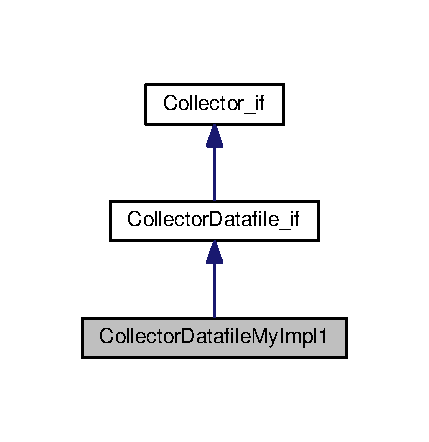
\includegraphics[width=206pt]{class_collector_datafile_my_impl1__inherit__graph}
\end{center}
\end{figure}


Collaboration diagram for Collector\-Datafile\-My\-Impl1\-:\nopagebreak
\begin{figure}[H]
\begin{center}
\leavevmode
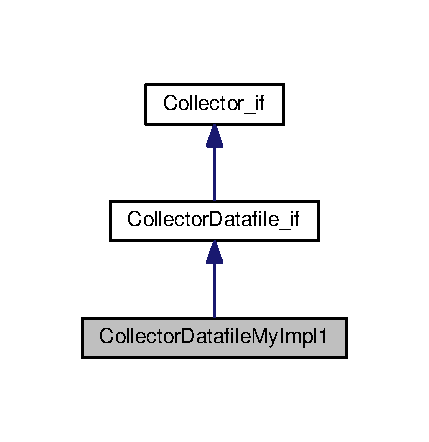
\includegraphics[width=206pt]{class_collector_datafile_my_impl1__coll__graph}
\end{center}
\end{figure}
\subsection*{Public Member Functions}
\begin{DoxyCompactItemize}
\item 
\hyperlink{class_collector_datafile_my_impl1_a88bec096f9b7d707bf436df5b2ab34e1}{Collector\-Datafile\-My\-Impl1} ()
\item 
\hyperlink{class_collector_datafile_my_impl1_a93b68a7b411573a7ff133856f22cbb1f}{Collector\-Datafile\-My\-Impl1} (const \hyperlink{class_collector_datafile_my_impl1}{Collector\-Datafile\-My\-Impl1} \&orig)
\item 
\hyperlink{class_collector_datafile_my_impl1_ac7362a33ec9e82bd3298068cc0c1c6f0}{$\sim$\-Collector\-Datafile\-My\-Impl1} ()
\item 
void \hyperlink{class_collector_datafile_my_impl1_a594004f005db5dd1122946445f4db70d}{clear} ()
\item 
void \hyperlink{class_collector_datafile_my_impl1_aa909fc87f2ee082512616840c9031365}{add\-Value} (double value)
\item 
double \hyperlink{class_collector_datafile_my_impl1_a5a29b2f71a4630c658fb83c047fb1054}{get\-Last\-Value} ()
\item 
unsigned long \hyperlink{class_collector_datafile_my_impl1_ac8ad59a3b664d082c8ca4fca9887148a}{num\-Elements} ()
\item 
double \hyperlink{class_collector_datafile_my_impl1_a55a505d56f9b95a55473bdf1ab24cffe}{get\-Value} (unsigned int num)
\item 
std\-::string \hyperlink{class_collector_datafile_my_impl1_a5ebe8076b9eb9816a1b7d823943102cf}{get\-Data\-Filename} ()
\item 
void \hyperlink{class_collector_datafile_my_impl1_ac4c401ae3cf4ccc723b6b9efa614ccd1}{set\-Data\-Filename} (std\-::string filename)
\end{DoxyCompactItemize}


\subsection{Detailed Description}


Definition at line 19 of file Collector\-Datafile\-My\-Impl1.\-h.



\subsection{Constructor \& Destructor Documentation}
\hypertarget{class_collector_datafile_my_impl1_a88bec096f9b7d707bf436df5b2ab34e1}{\index{Collector\-Datafile\-My\-Impl1@{Collector\-Datafile\-My\-Impl1}!Collector\-Datafile\-My\-Impl1@{Collector\-Datafile\-My\-Impl1}}
\index{Collector\-Datafile\-My\-Impl1@{Collector\-Datafile\-My\-Impl1}!CollectorDatafileMyImpl1@{Collector\-Datafile\-My\-Impl1}}
\subsubsection[{Collector\-Datafile\-My\-Impl1}]{\setlength{\rightskip}{0pt plus 5cm}Collector\-Datafile\-My\-Impl1\-::\-Collector\-Datafile\-My\-Impl1 (
\begin{DoxyParamCaption}
{}
\end{DoxyParamCaption}
)}}\label{class_collector_datafile_my_impl1_a88bec096f9b7d707bf436df5b2ab34e1}


Definition at line 16 of file Collector\-Datafile\-My\-Impl1.\-cpp.

\hypertarget{class_collector_datafile_my_impl1_a93b68a7b411573a7ff133856f22cbb1f}{\index{Collector\-Datafile\-My\-Impl1@{Collector\-Datafile\-My\-Impl1}!Collector\-Datafile\-My\-Impl1@{Collector\-Datafile\-My\-Impl1}}
\index{Collector\-Datafile\-My\-Impl1@{Collector\-Datafile\-My\-Impl1}!CollectorDatafileMyImpl1@{Collector\-Datafile\-My\-Impl1}}
\subsubsection[{Collector\-Datafile\-My\-Impl1}]{\setlength{\rightskip}{0pt plus 5cm}Collector\-Datafile\-My\-Impl1\-::\-Collector\-Datafile\-My\-Impl1 (
\begin{DoxyParamCaption}
\item[{const {\bf Collector\-Datafile\-My\-Impl1} \&}]{orig}
\end{DoxyParamCaption}
)}}\label{class_collector_datafile_my_impl1_a93b68a7b411573a7ff133856f22cbb1f}


Definition at line 19 of file Collector\-Datafile\-My\-Impl1.\-cpp.

\hypertarget{class_collector_datafile_my_impl1_ac7362a33ec9e82bd3298068cc0c1c6f0}{\index{Collector\-Datafile\-My\-Impl1@{Collector\-Datafile\-My\-Impl1}!$\sim$\-Collector\-Datafile\-My\-Impl1@{$\sim$\-Collector\-Datafile\-My\-Impl1}}
\index{$\sim$\-Collector\-Datafile\-My\-Impl1@{$\sim$\-Collector\-Datafile\-My\-Impl1}!CollectorDatafileMyImpl1@{Collector\-Datafile\-My\-Impl1}}
\subsubsection[{$\sim$\-Collector\-Datafile\-My\-Impl1}]{\setlength{\rightskip}{0pt plus 5cm}Collector\-Datafile\-My\-Impl1\-::$\sim$\-Collector\-Datafile\-My\-Impl1 (
\begin{DoxyParamCaption}
{}
\end{DoxyParamCaption}
)}}\label{class_collector_datafile_my_impl1_ac7362a33ec9e82bd3298068cc0c1c6f0}


Definition at line 22 of file Collector\-Datafile\-My\-Impl1.\-cpp.



\subsection{Member Function Documentation}
\hypertarget{class_collector_datafile_my_impl1_aa909fc87f2ee082512616840c9031365}{\index{Collector\-Datafile\-My\-Impl1@{Collector\-Datafile\-My\-Impl1}!add\-Value@{add\-Value}}
\index{add\-Value@{add\-Value}!CollectorDatafileMyImpl1@{Collector\-Datafile\-My\-Impl1}}
\subsubsection[{add\-Value}]{\setlength{\rightskip}{0pt plus 5cm}void Collector\-Datafile\-My\-Impl1\-::add\-Value (
\begin{DoxyParamCaption}
\item[{double}]{value}
\end{DoxyParamCaption}
)\hspace{0.3cm}{\ttfamily [virtual]}}}\label{class_collector_datafile_my_impl1_aa909fc87f2ee082512616840c9031365}


Implements \hyperlink{class_collector__if_ac7b83bce8ddb4903d247c1eddd656171}{Collector\-\_\-if}.



Definition at line 28 of file Collector\-Datafile\-My\-Impl1.\-cpp.

\hypertarget{class_collector_datafile_my_impl1_a594004f005db5dd1122946445f4db70d}{\index{Collector\-Datafile\-My\-Impl1@{Collector\-Datafile\-My\-Impl1}!clear@{clear}}
\index{clear@{clear}!CollectorDatafileMyImpl1@{Collector\-Datafile\-My\-Impl1}}
\subsubsection[{clear}]{\setlength{\rightskip}{0pt plus 5cm}void Collector\-Datafile\-My\-Impl1\-::clear (
\begin{DoxyParamCaption}
{}
\end{DoxyParamCaption}
)\hspace{0.3cm}{\ttfamily [virtual]}}}\label{class_collector_datafile_my_impl1_a594004f005db5dd1122946445f4db70d}


Implements \hyperlink{class_collector__if_a035bd1300c85866870c2f6178a9528e8}{Collector\-\_\-if}.



Definition at line 25 of file Collector\-Datafile\-My\-Impl1.\-cpp.

\hypertarget{class_collector_datafile_my_impl1_a5ebe8076b9eb9816a1b7d823943102cf}{\index{Collector\-Datafile\-My\-Impl1@{Collector\-Datafile\-My\-Impl1}!get\-Data\-Filename@{get\-Data\-Filename}}
\index{get\-Data\-Filename@{get\-Data\-Filename}!CollectorDatafileMyImpl1@{Collector\-Datafile\-My\-Impl1}}
\subsubsection[{get\-Data\-Filename}]{\setlength{\rightskip}{0pt plus 5cm}std\-::string Collector\-Datafile\-My\-Impl1\-::get\-Data\-Filename (
\begin{DoxyParamCaption}
{}
\end{DoxyParamCaption}
)\hspace{0.3cm}{\ttfamily [virtual]}}}\label{class_collector_datafile_my_impl1_a5ebe8076b9eb9816a1b7d823943102cf}


Implements \hyperlink{class_collector_datafile__if_a81d109f34c25f5295f76ba13f4234a3c}{Collector\-Datafile\-\_\-if}.



Definition at line 40 of file Collector\-Datafile\-My\-Impl1.\-cpp.

\hypertarget{class_collector_datafile_my_impl1_a5a29b2f71a4630c658fb83c047fb1054}{\index{Collector\-Datafile\-My\-Impl1@{Collector\-Datafile\-My\-Impl1}!get\-Last\-Value@{get\-Last\-Value}}
\index{get\-Last\-Value@{get\-Last\-Value}!CollectorDatafileMyImpl1@{Collector\-Datafile\-My\-Impl1}}
\subsubsection[{get\-Last\-Value}]{\setlength{\rightskip}{0pt plus 5cm}double Collector\-Datafile\-My\-Impl1\-::get\-Last\-Value (
\begin{DoxyParamCaption}
{}
\end{DoxyParamCaption}
)\hspace{0.3cm}{\ttfamily [virtual]}}}\label{class_collector_datafile_my_impl1_a5a29b2f71a4630c658fb83c047fb1054}


Implements \hyperlink{class_collector__if_aa14f7e1065af8fd38ab592e224fb7e43}{Collector\-\_\-if}.



Definition at line 31 of file Collector\-Datafile\-My\-Impl1.\-cpp.

\hypertarget{class_collector_datafile_my_impl1_a55a505d56f9b95a55473bdf1ab24cffe}{\index{Collector\-Datafile\-My\-Impl1@{Collector\-Datafile\-My\-Impl1}!get\-Value@{get\-Value}}
\index{get\-Value@{get\-Value}!CollectorDatafileMyImpl1@{Collector\-Datafile\-My\-Impl1}}
\subsubsection[{get\-Value}]{\setlength{\rightskip}{0pt plus 5cm}double Collector\-Datafile\-My\-Impl1\-::get\-Value (
\begin{DoxyParamCaption}
\item[{unsigned int}]{num}
\end{DoxyParamCaption}
)\hspace{0.3cm}{\ttfamily [virtual]}}}\label{class_collector_datafile_my_impl1_a55a505d56f9b95a55473bdf1ab24cffe}


Implements \hyperlink{class_collector_datafile__if_aa790efe68dfa16cebd66b481bbda8411}{Collector\-Datafile\-\_\-if}.



Definition at line 37 of file Collector\-Datafile\-My\-Impl1.\-cpp.

\hypertarget{class_collector_datafile_my_impl1_ac8ad59a3b664d082c8ca4fca9887148a}{\index{Collector\-Datafile\-My\-Impl1@{Collector\-Datafile\-My\-Impl1}!num\-Elements@{num\-Elements}}
\index{num\-Elements@{num\-Elements}!CollectorDatafileMyImpl1@{Collector\-Datafile\-My\-Impl1}}
\subsubsection[{num\-Elements}]{\setlength{\rightskip}{0pt plus 5cm}unsigned long Collector\-Datafile\-My\-Impl1\-::num\-Elements (
\begin{DoxyParamCaption}
{}
\end{DoxyParamCaption}
)\hspace{0.3cm}{\ttfamily [virtual]}}}\label{class_collector_datafile_my_impl1_ac8ad59a3b664d082c8ca4fca9887148a}


Implements \hyperlink{class_collector__if_a97fa632508ffdfad1365b3a949acf745}{Collector\-\_\-if}.



Definition at line 34 of file Collector\-Datafile\-My\-Impl1.\-cpp.

\hypertarget{class_collector_datafile_my_impl1_ac4c401ae3cf4ccc723b6b9efa614ccd1}{\index{Collector\-Datafile\-My\-Impl1@{Collector\-Datafile\-My\-Impl1}!set\-Data\-Filename@{set\-Data\-Filename}}
\index{set\-Data\-Filename@{set\-Data\-Filename}!CollectorDatafileMyImpl1@{Collector\-Datafile\-My\-Impl1}}
\subsubsection[{set\-Data\-Filename}]{\setlength{\rightskip}{0pt plus 5cm}void Collector\-Datafile\-My\-Impl1\-::set\-Data\-Filename (
\begin{DoxyParamCaption}
\item[{std\-::string}]{filename}
\end{DoxyParamCaption}
)\hspace{0.3cm}{\ttfamily [virtual]}}}\label{class_collector_datafile_my_impl1_ac4c401ae3cf4ccc723b6b9efa614ccd1}


Implements \hyperlink{class_collector_datafile__if_ab826bbf5472a5cfdbf2f2c30273da8eb}{Collector\-Datafile\-\_\-if}.



Definition at line 43 of file Collector\-Datafile\-My\-Impl1.\-cpp.



The documentation for this class was generated from the following files\-:\begin{DoxyCompactItemize}
\item 
\hyperlink{_collector_datafile_my_impl1_8h}{Collector\-Datafile\-My\-Impl1.\-h}\item 
\hyperlink{_collector_datafile_my_impl1_8cpp}{Collector\-Datafile\-My\-Impl1.\-cpp}\end{DoxyCompactItemize}

\hypertarget{class_collector_my_impl1}{\section{Collector\-My\-Impl1 Class Reference}
\label{class_collector_my_impl1}\index{Collector\-My\-Impl1@{Collector\-My\-Impl1}}
}


{\ttfamily \#include $<$Collector\-My\-Impl1.\-h$>$}



Inheritance diagram for Collector\-My\-Impl1\-:\nopagebreak
\begin{figure}[H]
\begin{center}
\leavevmode
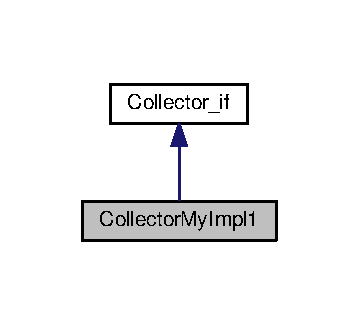
\includegraphics[width=172pt]{class_collector_my_impl1__inherit__graph}
\end{center}
\end{figure}


Collaboration diagram for Collector\-My\-Impl1\-:\nopagebreak
\begin{figure}[H]
\begin{center}
\leavevmode
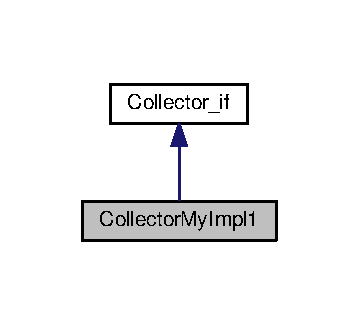
\includegraphics[width=172pt]{class_collector_my_impl1__coll__graph}
\end{center}
\end{figure}
\subsection*{Public Member Functions}
\begin{DoxyCompactItemize}
\item 
\hyperlink{class_collector_my_impl1_ab8d5d86d5d28f0cc3a4558fe5a6da56c}{Collector\-My\-Impl1} ()
\item 
\hyperlink{class_collector_my_impl1_a7d96fa7024ff2e2158613c4b55ea052f}{Collector\-My\-Impl1} (const \hyperlink{class_collector_my_impl1}{Collector\-My\-Impl1} \&orig)
\item 
\hyperlink{class_collector_my_impl1_a431e418b9b2cf55e6fb10ba688ae281e}{$\sim$\-Collector\-My\-Impl1} ()
\item 
void \hyperlink{class_collector_my_impl1_a9b570931955cafde878d6734aa914039}{clear} ()
\item 
void \hyperlink{class_collector_my_impl1_acc5d658a3429af8b7d4265cbc37485b5}{add\-Value} (double value)
\item 
double \hyperlink{class_collector_my_impl1_a56e754ba3175e2f335290e2a737e7104}{get\-Last\-Value} ()
\item 
unsigned int \hyperlink{class_collector_my_impl1_ac71aac361d3c9a5d0c9cc76c1c75e47e}{num\-Elements} ()
\end{DoxyCompactItemize}


\subsection{Constructor \& Destructor Documentation}
\hypertarget{class_collector_my_impl1_ab8d5d86d5d28f0cc3a4558fe5a6da56c}{\index{Collector\-My\-Impl1@{Collector\-My\-Impl1}!Collector\-My\-Impl1@{Collector\-My\-Impl1}}
\index{Collector\-My\-Impl1@{Collector\-My\-Impl1}!CollectorMyImpl1@{Collector\-My\-Impl1}}
\subsubsection[{Collector\-My\-Impl1}]{\setlength{\rightskip}{0pt plus 5cm}Collector\-My\-Impl1\-::\-Collector\-My\-Impl1 (
\begin{DoxyParamCaption}
{}
\end{DoxyParamCaption}
)}}\label{class_collector_my_impl1_ab8d5d86d5d28f0cc3a4558fe5a6da56c}
\hypertarget{class_collector_my_impl1_a7d96fa7024ff2e2158613c4b55ea052f}{\index{Collector\-My\-Impl1@{Collector\-My\-Impl1}!Collector\-My\-Impl1@{Collector\-My\-Impl1}}
\index{Collector\-My\-Impl1@{Collector\-My\-Impl1}!CollectorMyImpl1@{Collector\-My\-Impl1}}
\subsubsection[{Collector\-My\-Impl1}]{\setlength{\rightskip}{0pt plus 5cm}Collector\-My\-Impl1\-::\-Collector\-My\-Impl1 (
\begin{DoxyParamCaption}
\item[{const {\bf Collector\-My\-Impl1} \&}]{orig}
\end{DoxyParamCaption}
)}}\label{class_collector_my_impl1_a7d96fa7024ff2e2158613c4b55ea052f}
\hypertarget{class_collector_my_impl1_a431e418b9b2cf55e6fb10ba688ae281e}{\index{Collector\-My\-Impl1@{Collector\-My\-Impl1}!$\sim$\-Collector\-My\-Impl1@{$\sim$\-Collector\-My\-Impl1}}
\index{$\sim$\-Collector\-My\-Impl1@{$\sim$\-Collector\-My\-Impl1}!CollectorMyImpl1@{Collector\-My\-Impl1}}
\subsubsection[{$\sim$\-Collector\-My\-Impl1}]{\setlength{\rightskip}{0pt plus 5cm}Collector\-My\-Impl1\-::$\sim$\-Collector\-My\-Impl1 (
\begin{DoxyParamCaption}
{}
\end{DoxyParamCaption}
)}}\label{class_collector_my_impl1_a431e418b9b2cf55e6fb10ba688ae281e}


\subsection{Member Function Documentation}
\hypertarget{class_collector_my_impl1_acc5d658a3429af8b7d4265cbc37485b5}{\index{Collector\-My\-Impl1@{Collector\-My\-Impl1}!add\-Value@{add\-Value}}
\index{add\-Value@{add\-Value}!CollectorMyImpl1@{Collector\-My\-Impl1}}
\subsubsection[{add\-Value}]{\setlength{\rightskip}{0pt plus 5cm}void Collector\-My\-Impl1\-::add\-Value (
\begin{DoxyParamCaption}
\item[{double}]{value}
\end{DoxyParamCaption}
)\hspace{0.3cm}{\ttfamily [virtual]}}}\label{class_collector_my_impl1_acc5d658a3429af8b7d4265cbc37485b5}


Implements \hyperlink{class_collector__if_ac7b83bce8ddb4903d247c1eddd656171}{Collector\-\_\-if}.

\hypertarget{class_collector_my_impl1_a9b570931955cafde878d6734aa914039}{\index{Collector\-My\-Impl1@{Collector\-My\-Impl1}!clear@{clear}}
\index{clear@{clear}!CollectorMyImpl1@{Collector\-My\-Impl1}}
\subsubsection[{clear}]{\setlength{\rightskip}{0pt plus 5cm}void Collector\-My\-Impl1\-::clear (
\begin{DoxyParamCaption}
{}
\end{DoxyParamCaption}
)\hspace{0.3cm}{\ttfamily [virtual]}}}\label{class_collector_my_impl1_a9b570931955cafde878d6734aa914039}


Implements \hyperlink{class_collector__if_a035bd1300c85866870c2f6178a9528e8}{Collector\-\_\-if}.

\hypertarget{class_collector_my_impl1_a56e754ba3175e2f335290e2a737e7104}{\index{Collector\-My\-Impl1@{Collector\-My\-Impl1}!get\-Last\-Value@{get\-Last\-Value}}
\index{get\-Last\-Value@{get\-Last\-Value}!CollectorMyImpl1@{Collector\-My\-Impl1}}
\subsubsection[{get\-Last\-Value}]{\setlength{\rightskip}{0pt plus 5cm}double Collector\-My\-Impl1\-::get\-Last\-Value (
\begin{DoxyParamCaption}
{}
\end{DoxyParamCaption}
)\hspace{0.3cm}{\ttfamily [virtual]}}}\label{class_collector_my_impl1_a56e754ba3175e2f335290e2a737e7104}


Implements \hyperlink{class_collector__if_aa14f7e1065af8fd38ab592e224fb7e43}{Collector\-\_\-if}.

\hypertarget{class_collector_my_impl1_ac71aac361d3c9a5d0c9cc76c1c75e47e}{\index{Collector\-My\-Impl1@{Collector\-My\-Impl1}!num\-Elements@{num\-Elements}}
\index{num\-Elements@{num\-Elements}!CollectorMyImpl1@{Collector\-My\-Impl1}}
\subsubsection[{num\-Elements}]{\setlength{\rightskip}{0pt plus 5cm}unsigned int Collector\-My\-Impl1\-::num\-Elements (
\begin{DoxyParamCaption}
{}
\end{DoxyParamCaption}
)\hspace{0.3cm}{\ttfamily [virtual]}}}\label{class_collector_my_impl1_ac71aac361d3c9a5d0c9cc76c1c75e47e}


Implements \hyperlink{class_collector__if_a75c20c68c54089105ca8c440997a7cca}{Collector\-\_\-if}.



The documentation for this class was generated from the following files\-:\begin{DoxyCompactItemize}
\item 
\hyperlink{_collector_my_impl1_8h}{Collector\-My\-Impl1.\-h}\item 
\hyperlink{_collector_my_impl1_8cpp}{Collector\-My\-Impl1.\-cpp}\end{DoxyCompactItemize}

\hypertarget{class_create}{}\section{Create Class Reference}
\label{class_create}\index{Create@{Create}}


{\ttfamily \#include $<$Create.\+h$>$}



Inheritance diagram for Create\+:\nopagebreak
\begin{figure}[H]
\begin{center}
\leavevmode
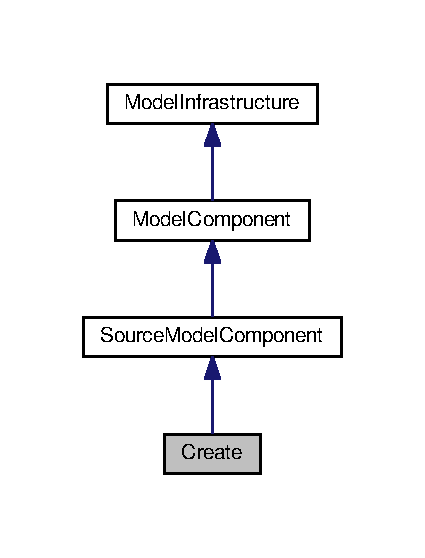
\includegraphics[width=204pt]{class_create__inherit__graph}
\end{center}
\end{figure}


Collaboration diagram for Create\+:\nopagebreak
\begin{figure}[H]
\begin{center}
\leavevmode
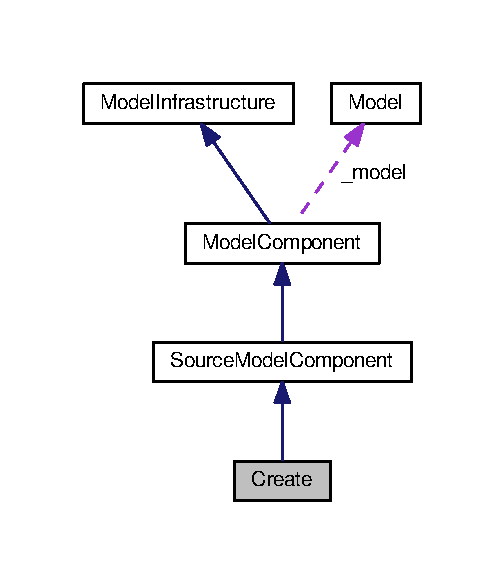
\includegraphics[width=256pt]{class_create__coll__graph}
\end{center}
\end{figure}
\subsection*{Public Member Functions}
\begin{DoxyCompactItemize}
\item 
\hyperlink{class_create_a81bd7a50b926660c264ebe29e2095170}{Create} (\hyperlink{class_model}{Model} $\ast$model)
\item 
\hyperlink{class_create_a035a6f7ddd02dace181b23913b91bad9}{Create} (const \hyperlink{class_create}{Create} \&orig)
\item 
virtual \hyperlink{class_create_a6060fda2b105228446ddddb09f63d127}{$\sim$\+Create} ()
\item 
virtual std\+::string \hyperlink{class_create_a8d1832d2165bbeea4a5a88aded883f86}{show} ()
\end{DoxyCompactItemize}
\subsection*{Protected Member Functions}
\begin{DoxyCompactItemize}
\item 
virtual void \hyperlink{class_create_acd3a4b8805561591e0c88d3fd689cf74}{\+\_\+execute} (\hyperlink{class_entity}{Entity} $\ast$entity)
\item 
virtual void \hyperlink{class_create_aaa3cb1a4359586b0b8df817f57916286}{\+\_\+load\+Instance} (std\+::list$<$ std\+::string $>$ words)
\item 
virtual std\+::list$<$ std\+::string $>$ $\ast$ \hyperlink{class_create_ae1fd0c281cec35dcf91881acba8d7041}{\+\_\+save\+Instance} ()
\item 
virtual bool \hyperlink{class_create_ad445fd3bec94b4e66669089f10f96057}{\+\_\+verify\+Symbols} (std\+::string $\ast$error\+Message)
\end{DoxyCompactItemize}
\subsection*{Additional Inherited Members}


\subsection{Detailed Description}
\hyperlink{class_create}{Create} is the most basic component to include the first entities into the model, and therefore is a source component (derived from \hyperlink{class_source_model_component}{Source\+Model\+Component}) 

\subsection{Constructor \& Destructor Documentation}
\index{Create@{Create}!Create@{Create}}
\index{Create@{Create}!Create@{Create}}
\subsubsection[{\texorpdfstring{Create(\+Model $\ast$model)}{Create(Model *model)}}]{\setlength{\rightskip}{0pt plus 5cm}Create\+::\+Create (
\begin{DoxyParamCaption}
\item[{{\bf Model} $\ast$}]{model}
\end{DoxyParamCaption}
)}\hypertarget{class_create_a81bd7a50b926660c264ebe29e2095170}{}\label{class_create_a81bd7a50b926660c264ebe29e2095170}


Here is the call graph for this function\+:\nopagebreak
\begin{figure}[H]
\begin{center}
\leavevmode
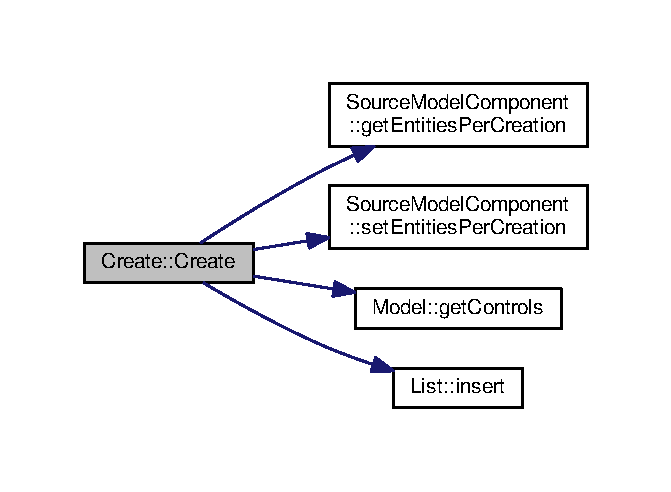
\includegraphics[width=321pt]{class_create_a81bd7a50b926660c264ebe29e2095170_cgraph}
\end{center}
\end{figure}


\index{Create@{Create}!Create@{Create}}
\index{Create@{Create}!Create@{Create}}
\subsubsection[{\texorpdfstring{Create(const Create \&orig)}{Create(const Create &orig)}}]{\setlength{\rightskip}{0pt plus 5cm}Create\+::\+Create (
\begin{DoxyParamCaption}
\item[{const {\bf Create} \&}]{orig}
\end{DoxyParamCaption}
)}\hypertarget{class_create_a035a6f7ddd02dace181b23913b91bad9}{}\label{class_create_a035a6f7ddd02dace181b23913b91bad9}
\index{Create@{Create}!````~Create@{$\sim$\+Create}}
\index{````~Create@{$\sim$\+Create}!Create@{Create}}
\subsubsection[{\texorpdfstring{$\sim$\+Create()}{~Create()}}]{\setlength{\rightskip}{0pt plus 5cm}Create\+::$\sim$\+Create (
\begin{DoxyParamCaption}
{}
\end{DoxyParamCaption}
)\hspace{0.3cm}{\ttfamily [virtual]}}\hypertarget{class_create_a6060fda2b105228446ddddb09f63d127}{}\label{class_create_a6060fda2b105228446ddddb09f63d127}


\subsection{Member Function Documentation}
\index{Create@{Create}!\+\_\+execute@{\+\_\+execute}}
\index{\+\_\+execute@{\+\_\+execute}!Create@{Create}}
\subsubsection[{\texorpdfstring{\+\_\+execute(\+Entity $\ast$entity)}{_execute(Entity *entity)}}]{\setlength{\rightskip}{0pt plus 5cm}void Create\+::\+\_\+execute (
\begin{DoxyParamCaption}
\item[{{\bf Entity} $\ast$}]{entity}
\end{DoxyParamCaption}
)\hspace{0.3cm}{\ttfamily [protected]}, {\ttfamily [virtual]}}\hypertarget{class_create_acd3a4b8805561591e0c88d3fd689cf74}{}\label{class_create_acd3a4b8805561591e0c88d3fd689cf74}


Implements \hyperlink{class_model_component_ae3fcf8bbdd8368c882438424aa73f714}{Model\+Component}.



Here is the call graph for this function\+:\nopagebreak
\begin{figure}[H]
\begin{center}
\leavevmode
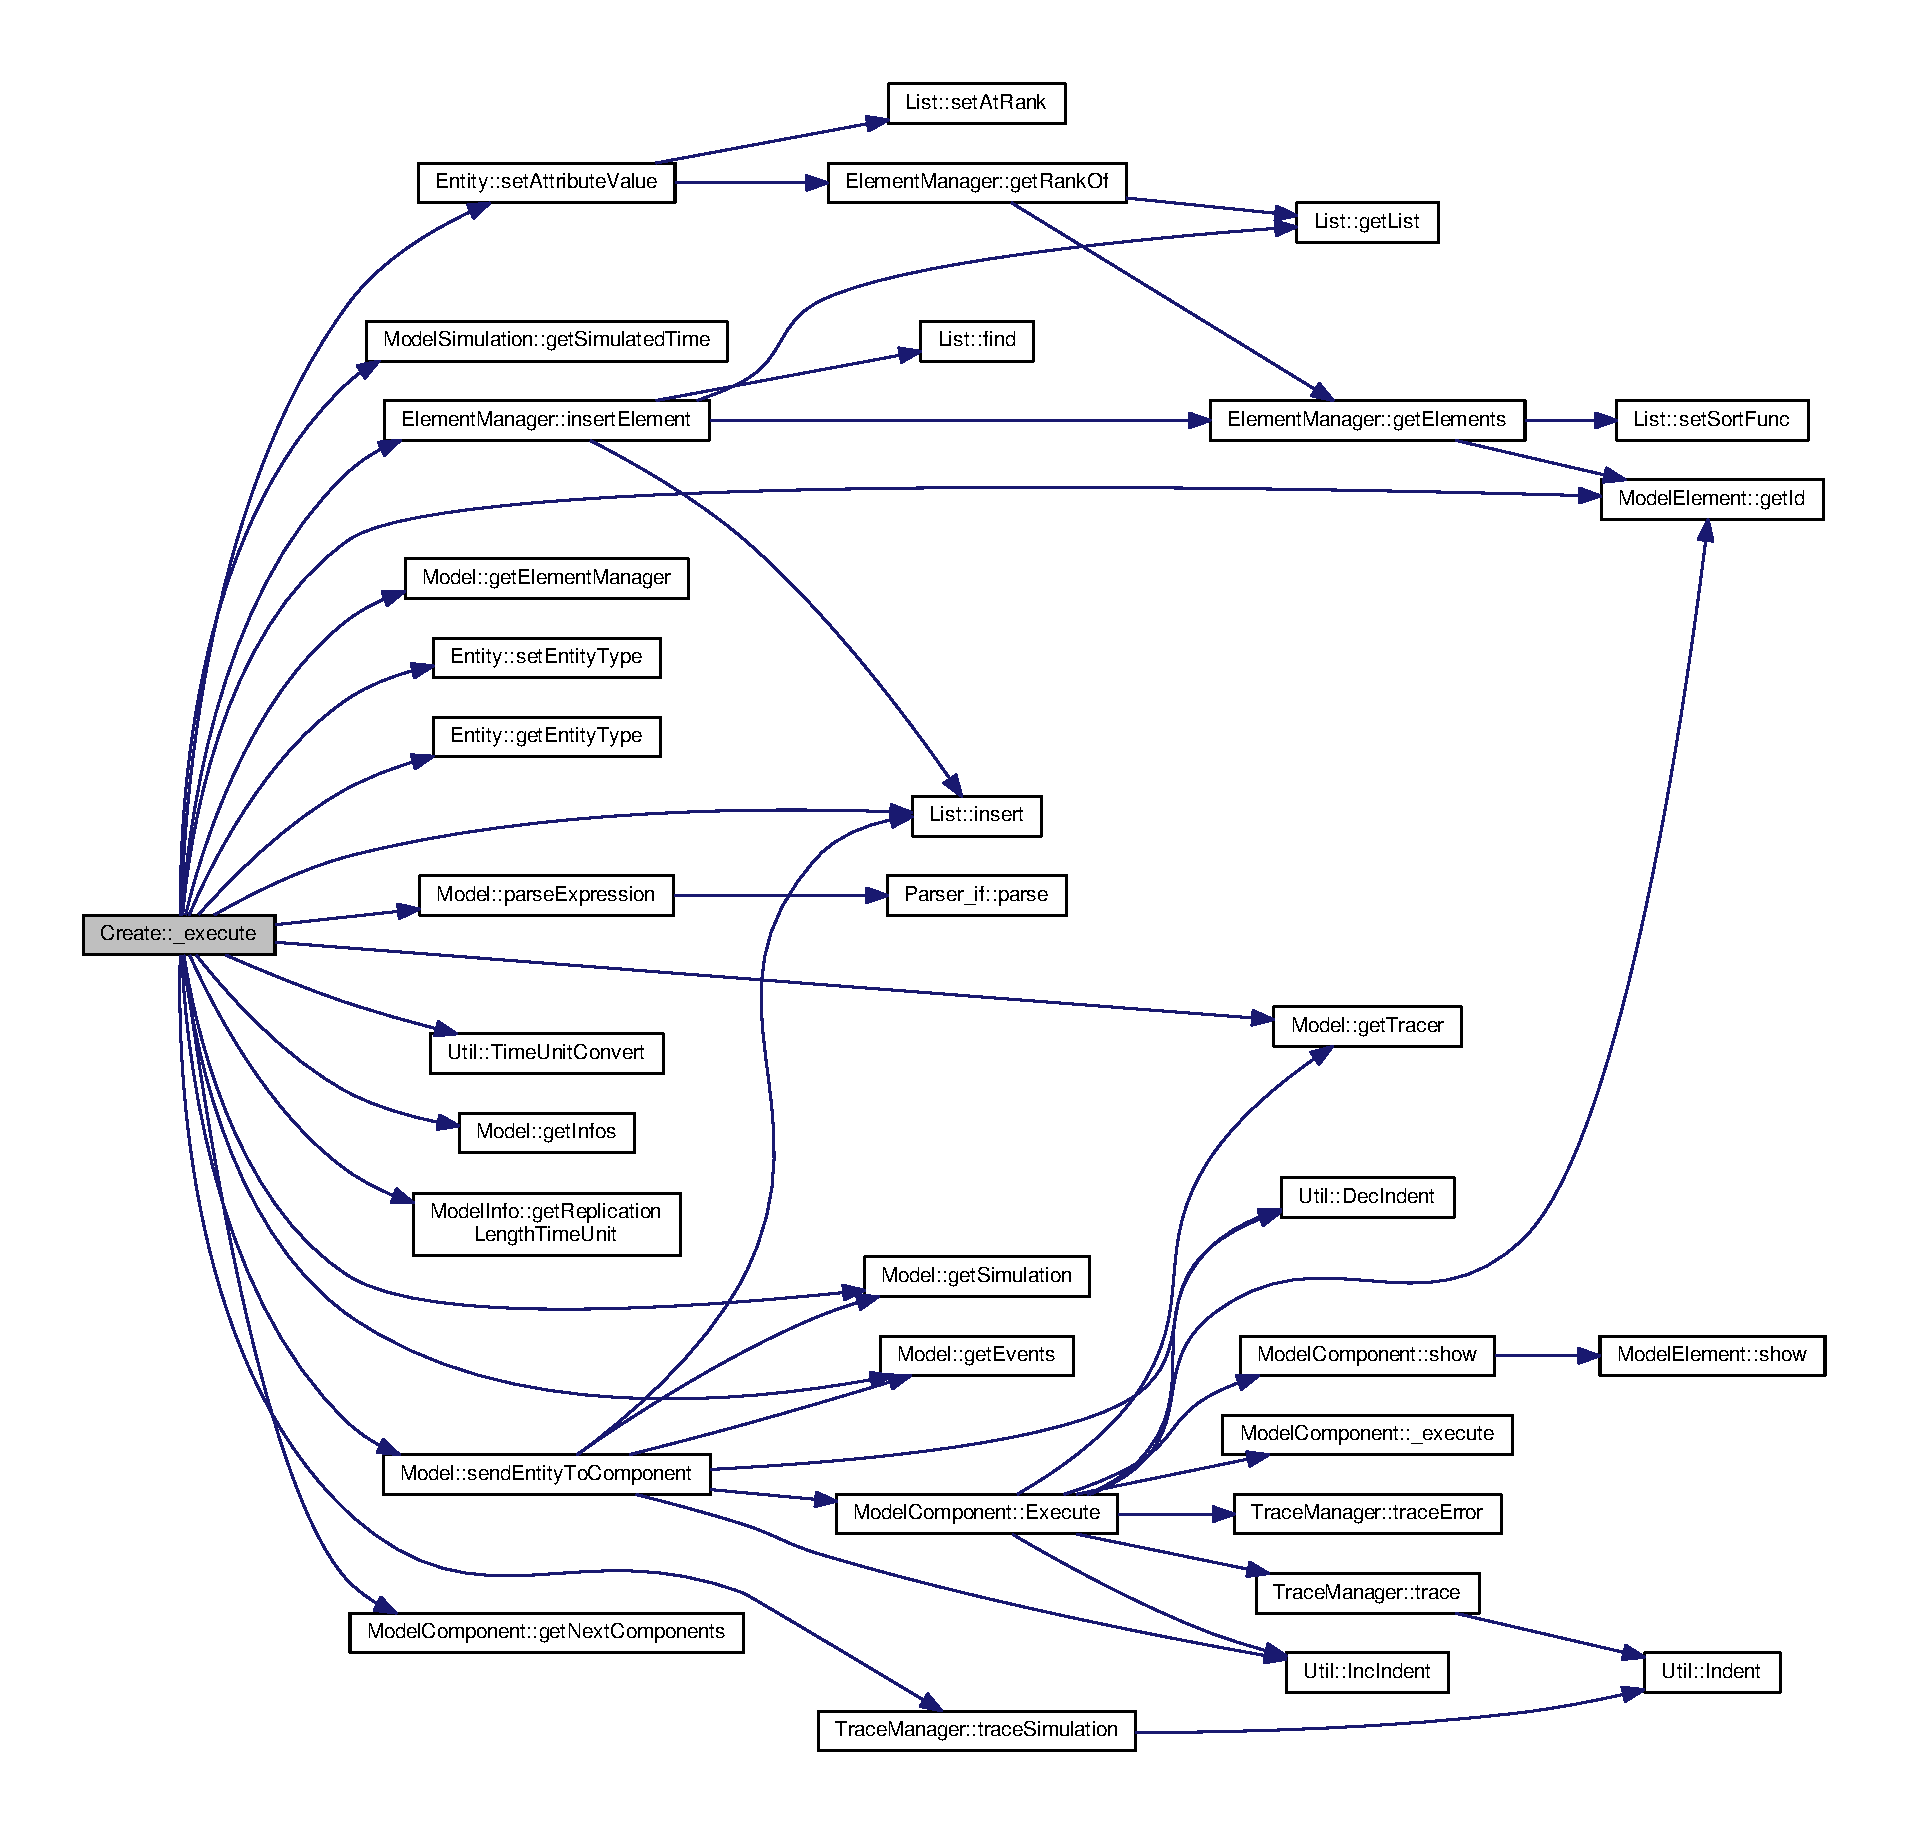
\includegraphics[width=350pt]{class_create_acd3a4b8805561591e0c88d3fd689cf74_cgraph}
\end{center}
\end{figure}


\index{Create@{Create}!\+\_\+load\+Instance@{\+\_\+load\+Instance}}
\index{\+\_\+load\+Instance@{\+\_\+load\+Instance}!Create@{Create}}
\subsubsection[{\texorpdfstring{\+\_\+load\+Instance(std\+::list$<$ std\+::string $>$ words)}{_loadInstance(std::list< std::string > words)}}]{\setlength{\rightskip}{0pt plus 5cm}void Create\+::\+\_\+load\+Instance (
\begin{DoxyParamCaption}
\item[{std\+::list$<$ std\+::string $>$}]{words}
\end{DoxyParamCaption}
)\hspace{0.3cm}{\ttfamily [protected]}, {\ttfamily [virtual]}}\hypertarget{class_create_aaa3cb1a4359586b0b8df817f57916286}{}\label{class_create_aaa3cb1a4359586b0b8df817f57916286}


Implements \hyperlink{class_model_element_a8208ee1dbd8b15acf7c2a0a85b218d56}{Model\+Element}.



Here is the call graph for this function\+:\nopagebreak
\begin{figure}[H]
\begin{center}
\leavevmode
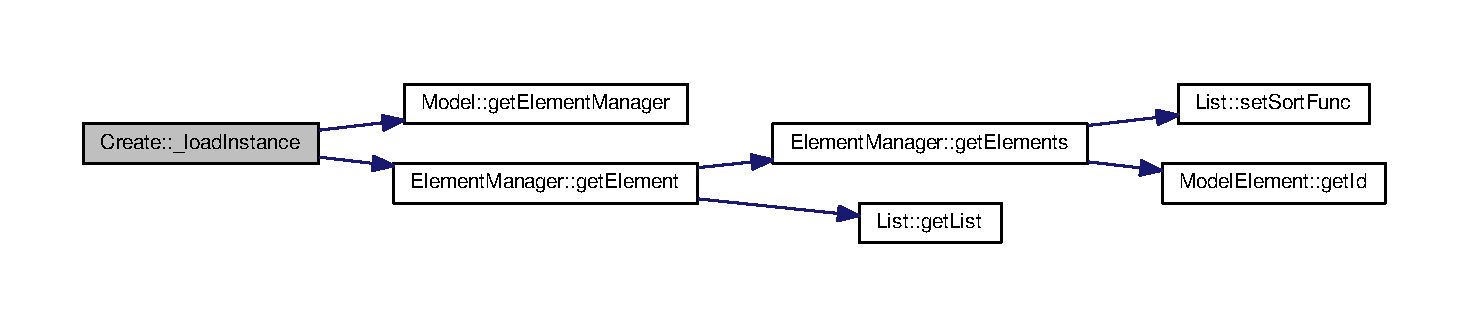
\includegraphics[width=350pt]{class_create_aaa3cb1a4359586b0b8df817f57916286_cgraph}
\end{center}
\end{figure}


\index{Create@{Create}!\+\_\+save\+Instance@{\+\_\+save\+Instance}}
\index{\+\_\+save\+Instance@{\+\_\+save\+Instance}!Create@{Create}}
\subsubsection[{\texorpdfstring{\+\_\+save\+Instance()}{_saveInstance()}}]{\setlength{\rightskip}{0pt plus 5cm}std\+::list$<$ std\+::string $>$ $\ast$ Create\+::\+\_\+save\+Instance (
\begin{DoxyParamCaption}
{}
\end{DoxyParamCaption}
)\hspace{0.3cm}{\ttfamily [protected]}, {\ttfamily [virtual]}}\hypertarget{class_create_ae1fd0c281cec35dcf91881acba8d7041}{}\label{class_create_ae1fd0c281cec35dcf91881acba8d7041}


Reimplemented from \hyperlink{class_model_component_a465f41c7191cb0fdf9039ef1f3d755a5}{Model\+Component}.



Here is the call graph for this function\+:\nopagebreak
\begin{figure}[H]
\begin{center}
\leavevmode
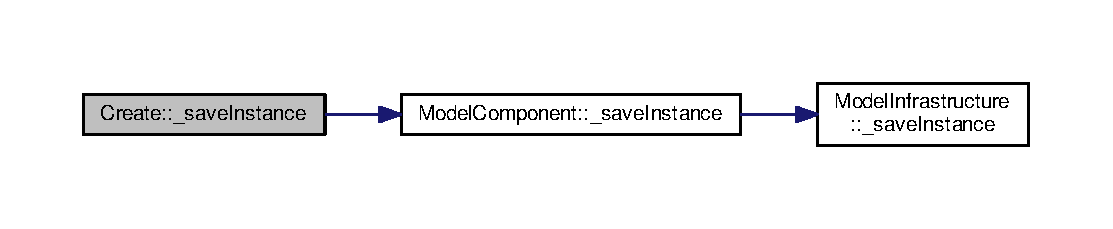
\includegraphics[width=350pt]{class_create_ae1fd0c281cec35dcf91881acba8d7041_cgraph}
\end{center}
\end{figure}


\index{Create@{Create}!\+\_\+verify\+Symbols@{\+\_\+verify\+Symbols}}
\index{\+\_\+verify\+Symbols@{\+\_\+verify\+Symbols}!Create@{Create}}
\subsubsection[{\texorpdfstring{\+\_\+verify\+Symbols(std\+::string $\ast$error\+Message)}{_verifySymbols(std::string *errorMessage)}}]{\setlength{\rightskip}{0pt plus 5cm}bool Create\+::\+\_\+verify\+Symbols (
\begin{DoxyParamCaption}
\item[{std\+::string $\ast$}]{error\+Message}
\end{DoxyParamCaption}
)\hspace{0.3cm}{\ttfamily [protected]}, {\ttfamily [virtual]}}\hypertarget{class_create_ad445fd3bec94b4e66669089f10f96057}{}\label{class_create_ad445fd3bec94b4e66669089f10f96057}


Implements \hyperlink{class_model_element_a42d23a83672cf746c709a031966484b2}{Model\+Element}.



Here is the call graph for this function\+:\nopagebreak
\begin{figure}[H]
\begin{center}
\leavevmode
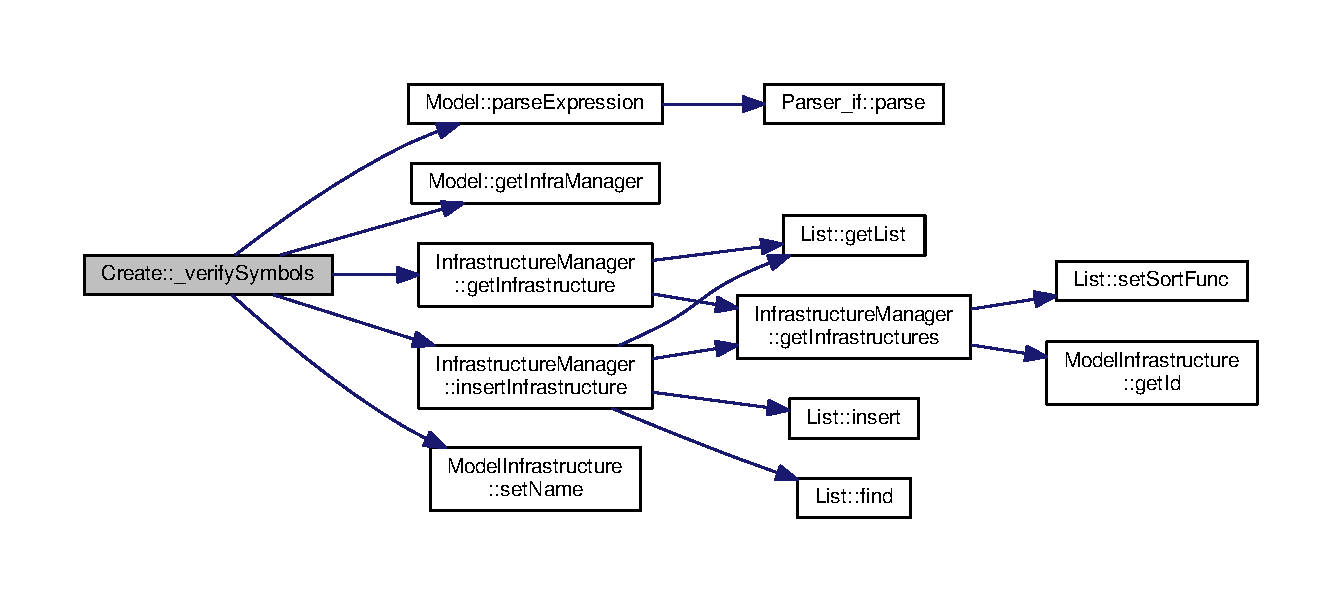
\includegraphics[width=350pt]{class_create_ad445fd3bec94b4e66669089f10f96057_cgraph}
\end{center}
\end{figure}


\index{Create@{Create}!show@{show}}
\index{show@{show}!Create@{Create}}
\subsubsection[{\texorpdfstring{show()}{show()}}]{\setlength{\rightskip}{0pt plus 5cm}std\+::string Create\+::show (
\begin{DoxyParamCaption}
{}
\end{DoxyParamCaption}
)\hspace{0.3cm}{\ttfamily [virtual]}}\hypertarget{class_create_a8d1832d2165bbeea4a5a88aded883f86}{}\label{class_create_a8d1832d2165bbeea4a5a88aded883f86}


Reimplemented from \hyperlink{class_source_model_component_a4011597b5780fcc0495e8e22ab8158f6}{Source\+Model\+Component}.



Here is the call graph for this function\+:\nopagebreak
\begin{figure}[H]
\begin{center}
\leavevmode
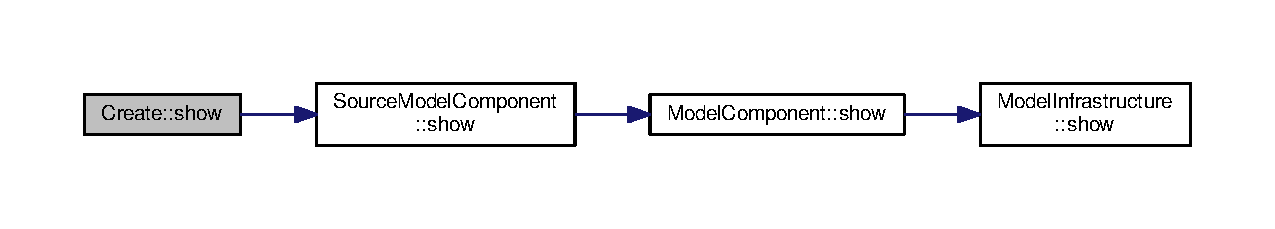
\includegraphics[width=350pt]{class_create_a8d1832d2165bbeea4a5a88aded883f86_cgraph}
\end{center}
\end{figure}




The documentation for this class was generated from the following files\+:\begin{DoxyCompactItemize}
\item 
\hyperlink{_create_8h}{Create.\+h}\item 
\hyperlink{_create_8cpp}{Create.\+cpp}\end{DoxyCompactItemize}

\hypertarget{class_delay}{\section{Delay Class Reference}
\label{class_delay}\index{Delay@{Delay}}
}


{\ttfamily \#include $<$Delay.\-h$>$}



Inheritance diagram for Delay\-:\nopagebreak
\begin{figure}[H]
\begin{center}
\leavevmode
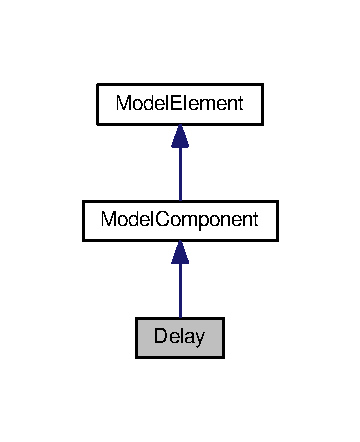
\includegraphics[width=180pt]{class_delay__inherit__graph}
\end{center}
\end{figure}


Collaboration diagram for Delay\-:\nopagebreak
\begin{figure}[H]
\begin{center}
\leavevmode
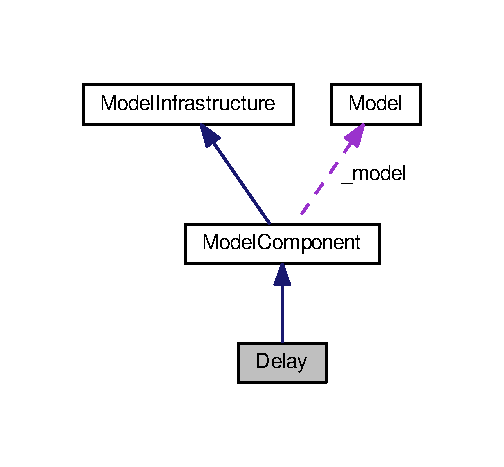
\includegraphics[width=241pt]{class_delay__coll__graph}
\end{center}
\end{figure}
\subsection*{Public Member Functions}
\begin{DoxyCompactItemize}
\item 
\hyperlink{class_delay_a155ad32911b3289d968cca746f940520}{Delay} (\hyperlink{class_model}{Model} $\ast$model)
\item 
\hyperlink{class_delay_a5892fd8feb283f11980c0a9adb9befa7}{Delay} (const \hyperlink{class_delay}{Delay} \&orig)
\item 
virtual \hyperlink{class_delay_afee934130955d45563a6c5baaaf052d2}{$\sim$\-Delay} ()
\item 
void \hyperlink{class_delay_a683b53af607a424477acb946eb3afdfc}{set\-Delay\-Expression} (std\-::string \-\_\-delay\-Expression)
\item 
std\-::string \hyperlink{class_delay_a58559eda9ed25330d29b967c1bb0add5}{get\-Delay\-Expression} () const 
\item 
void \hyperlink{class_delay_abe7e89dba0974a81d00e6d2c0548fc1e}{set\-Delay\-Time\-Unit} (\hyperlink{class_util_aadbd82055afeaa7d4fb4da513de628ff}{Util\-::\-Time\-Unit} \-\_\-delay\-Time\-Unit)
\item 
\hyperlink{class_util_aadbd82055afeaa7d4fb4da513de628ff}{Util\-::\-Time\-Unit} \hyperlink{class_delay_a0561a6fdb4dd317952b5bb8d87b0c15f}{get\-Delay\-Time\-Unit} () const 
\item 
virtual std\-::string \hyperlink{class_delay_af8187e4515417b547dc22b5ee0a1f95d}{show} ()
\end{DoxyCompactItemize}
\subsection*{Protected Member Functions}
\begin{DoxyCompactItemize}
\item 
virtual void \hyperlink{class_delay_a029d91a2cd736ff9c361c69336e6ab41}{\-\_\-execute} (\hyperlink{class_entity}{Entity} $\ast$entity)
\item 
virtual void \hyperlink{class_delay_acd33d05fc1c8d6d66a6f674e49ee7c61}{\-\_\-load\-Instance} (std\-::list$<$ std\-::string $>$ words)
\item 
virtual std\-::list$<$ std\-::string $>$ $\ast$ \hyperlink{class_delay_a73676f11cddd31439a407b5dabcea43a}{\-\_\-save\-Instance} ()
\item 
virtual bool \hyperlink{class_delay_af1690df9ba58e9972f5721f5bdc2b520}{\-\_\-verify\-Symbols} (std\-::string $\ast$error\-Message)
\end{DoxyCompactItemize}
\subsection*{Additional Inherited Members}


\subsection{Detailed Description}


Definition at line 20 of file Delay.\-h.



\subsection{Constructor \& Destructor Documentation}
\hypertarget{class_delay_a155ad32911b3289d968cca746f940520}{\index{Delay@{Delay}!Delay@{Delay}}
\index{Delay@{Delay}!Delay@{Delay}}
\subsubsection[{Delay}]{\setlength{\rightskip}{0pt plus 5cm}Delay\-::\-Delay (
\begin{DoxyParamCaption}
\item[{{\bf Model} $\ast$}]{model}
\end{DoxyParamCaption}
)}}\label{class_delay_a155ad32911b3289d968cca746f940520}


Definition at line 17 of file Delay.\-cpp.

\hypertarget{class_delay_a5892fd8feb283f11980c0a9adb9befa7}{\index{Delay@{Delay}!Delay@{Delay}}
\index{Delay@{Delay}!Delay@{Delay}}
\subsubsection[{Delay}]{\setlength{\rightskip}{0pt plus 5cm}Delay\-::\-Delay (
\begin{DoxyParamCaption}
\item[{const {\bf Delay} \&}]{orig}
\end{DoxyParamCaption}
)}}\label{class_delay_a5892fd8feb283f11980c0a9adb9befa7}


Definition at line 21 of file Delay.\-cpp.

\hypertarget{class_delay_afee934130955d45563a6c5baaaf052d2}{\index{Delay@{Delay}!$\sim$\-Delay@{$\sim$\-Delay}}
\index{$\sim$\-Delay@{$\sim$\-Delay}!Delay@{Delay}}
\subsubsection[{$\sim$\-Delay}]{\setlength{\rightskip}{0pt plus 5cm}Delay\-::$\sim$\-Delay (
\begin{DoxyParamCaption}
{}
\end{DoxyParamCaption}
)\hspace{0.3cm}{\ttfamily [virtual]}}}\label{class_delay_afee934130955d45563a6c5baaaf052d2}


Definition at line 24 of file Delay.\-cpp.



\subsection{Member Function Documentation}
\hypertarget{class_delay_a029d91a2cd736ff9c361c69336e6ab41}{\index{Delay@{Delay}!\-\_\-execute@{\-\_\-execute}}
\index{\-\_\-execute@{\-\_\-execute}!Delay@{Delay}}
\subsubsection[{\-\_\-execute}]{\setlength{\rightskip}{0pt plus 5cm}void Delay\-::\-\_\-execute (
\begin{DoxyParamCaption}
\item[{{\bf Entity} $\ast$}]{entity}
\end{DoxyParamCaption}
)\hspace{0.3cm}{\ttfamily [protected]}, {\ttfamily [virtual]}}}\label{class_delay_a029d91a2cd736ff9c361c69336e6ab41}


Implements \hyperlink{class_model_component_ae3fcf8bbdd8368c882438424aa73f714}{Model\-Component}.



Definition at line 49 of file Delay.\-cpp.



Here is the call graph for this function\-:\nopagebreak
\begin{figure}[H]
\begin{center}
\leavevmode
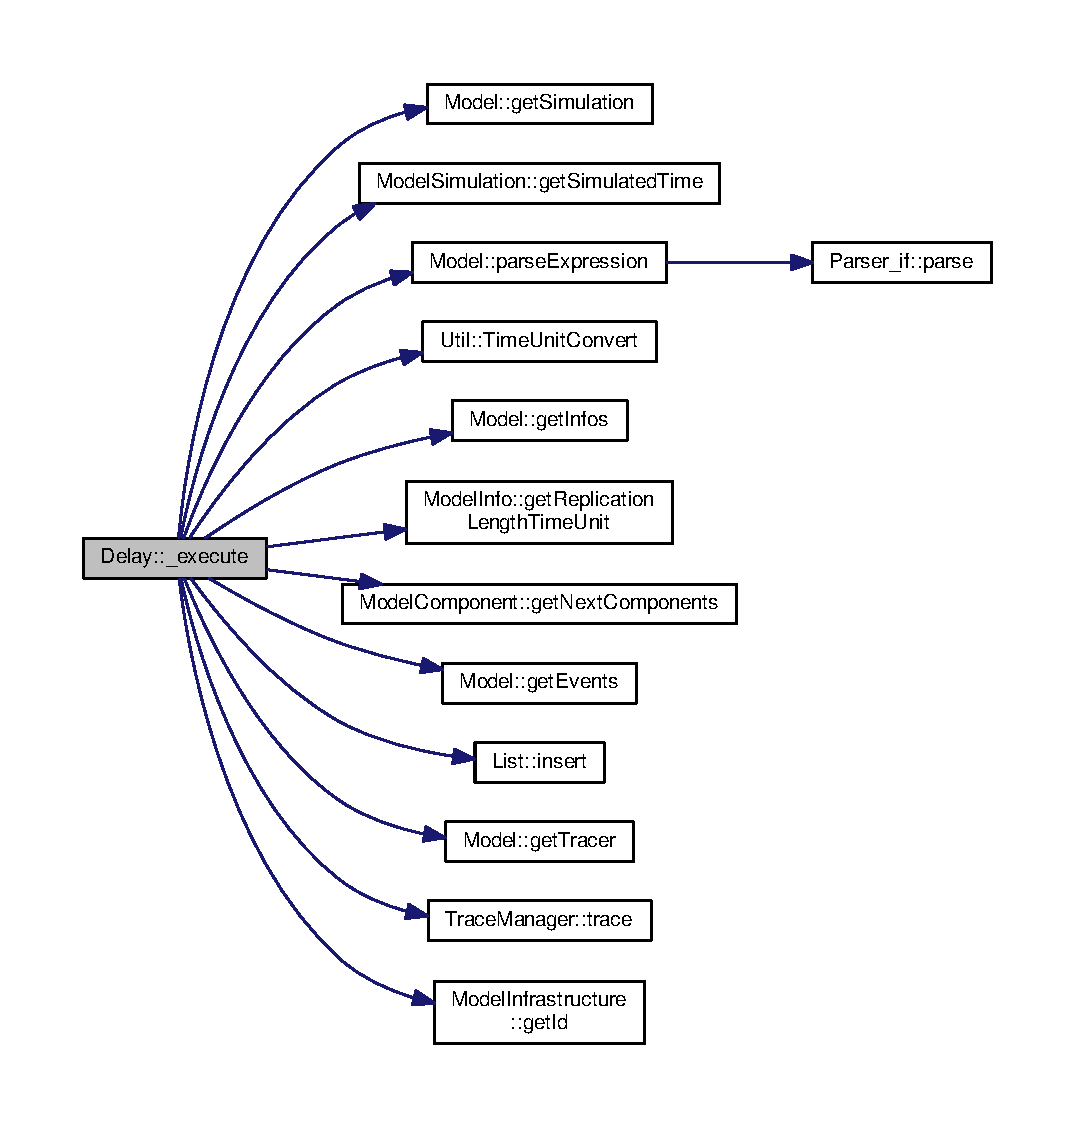
\includegraphics[width=350pt]{class_delay_a029d91a2cd736ff9c361c69336e6ab41_cgraph}
\end{center}
\end{figure}


\hypertarget{class_delay_acd33d05fc1c8d6d66a6f674e49ee7c61}{\index{Delay@{Delay}!\-\_\-load\-Instance@{\-\_\-load\-Instance}}
\index{\-\_\-load\-Instance@{\-\_\-load\-Instance}!Delay@{Delay}}
\subsubsection[{\-\_\-load\-Instance}]{\setlength{\rightskip}{0pt plus 5cm}void Delay\-::\-\_\-load\-Instance (
\begin{DoxyParamCaption}
\item[{std\-::list$<$ std\-::string $>$}]{words}
\end{DoxyParamCaption}
)\hspace{0.3cm}{\ttfamily [protected]}, {\ttfamily [virtual]}}}\label{class_delay_acd33d05fc1c8d6d66a6f674e49ee7c61}


Implements \hyperlink{class_model_infrastructure_ae118c8ad2ac9d4397c40d004af51b2dc}{Model\-Infrastructure}.



Definition at line 58 of file Delay.\-cpp.

\hypertarget{class_delay_a73676f11cddd31439a407b5dabcea43a}{\index{Delay@{Delay}!\-\_\-save\-Instance@{\-\_\-save\-Instance}}
\index{\-\_\-save\-Instance@{\-\_\-save\-Instance}!Delay@{Delay}}
\subsubsection[{\-\_\-save\-Instance}]{\setlength{\rightskip}{0pt plus 5cm}std\-::list$<$ std\-::string $>$ $\ast$ Delay\-::\-\_\-save\-Instance (
\begin{DoxyParamCaption}
{}
\end{DoxyParamCaption}
)\hspace{0.3cm}{\ttfamily [protected]}, {\ttfamily [virtual]}}}\label{class_delay_a73676f11cddd31439a407b5dabcea43a}


Implements \hyperlink{class_model_infrastructure_a3da2fd381c44752598bc448b207e8287}{Model\-Infrastructure}.



Definition at line 62 of file Delay.\-cpp.

\hypertarget{class_delay_af1690df9ba58e9972f5721f5bdc2b520}{\index{Delay@{Delay}!\-\_\-verify\-Symbols@{\-\_\-verify\-Symbols}}
\index{\-\_\-verify\-Symbols@{\-\_\-verify\-Symbols}!Delay@{Delay}}
\subsubsection[{\-\_\-verify\-Symbols}]{\setlength{\rightskip}{0pt plus 5cm}bool Delay\-::\-\_\-verify\-Symbols (
\begin{DoxyParamCaption}
\item[{std\-::string $\ast$}]{error\-Message}
\end{DoxyParamCaption}
)\hspace{0.3cm}{\ttfamily [protected]}, {\ttfamily [virtual]}}}\label{class_delay_af1690df9ba58e9972f5721f5bdc2b520}


Implements \hyperlink{class_model_infrastructure_a43de089b35b96c32dd24ca4f9636a388}{Model\-Infrastructure}.



Definition at line 68 of file Delay.\-cpp.

\hypertarget{class_delay_a58559eda9ed25330d29b967c1bb0add5}{\index{Delay@{Delay}!get\-Delay\-Expression@{get\-Delay\-Expression}}
\index{get\-Delay\-Expression@{get\-Delay\-Expression}!Delay@{Delay}}
\subsubsection[{get\-Delay\-Expression}]{\setlength{\rightskip}{0pt plus 5cm}std\-::string Delay\-::get\-Delay\-Expression (
\begin{DoxyParamCaption}
{}
\end{DoxyParamCaption}
) const}}\label{class_delay_a58559eda9ed25330d29b967c1bb0add5}


Definition at line 37 of file Delay.\-cpp.

\hypertarget{class_delay_a0561a6fdb4dd317952b5bb8d87b0c15f}{\index{Delay@{Delay}!get\-Delay\-Time\-Unit@{get\-Delay\-Time\-Unit}}
\index{get\-Delay\-Time\-Unit@{get\-Delay\-Time\-Unit}!Delay@{Delay}}
\subsubsection[{get\-Delay\-Time\-Unit}]{\setlength{\rightskip}{0pt plus 5cm}{\bf Util\-::\-Time\-Unit} Delay\-::get\-Delay\-Time\-Unit (
\begin{DoxyParamCaption}
{}
\end{DoxyParamCaption}
) const}}\label{class_delay_a0561a6fdb4dd317952b5bb8d87b0c15f}


Definition at line 45 of file Delay.\-cpp.

\hypertarget{class_delay_a683b53af607a424477acb946eb3afdfc}{\index{Delay@{Delay}!set\-Delay\-Expression@{set\-Delay\-Expression}}
\index{set\-Delay\-Expression@{set\-Delay\-Expression}!Delay@{Delay}}
\subsubsection[{set\-Delay\-Expression}]{\setlength{\rightskip}{0pt plus 5cm}void Delay\-::set\-Delay\-Expression (
\begin{DoxyParamCaption}
\item[{std\-::string}]{\-\_\-delay\-Expression}
\end{DoxyParamCaption}
)}}\label{class_delay_a683b53af607a424477acb946eb3afdfc}


Definition at line 33 of file Delay.\-cpp.



Here is the caller graph for this function\-:\nopagebreak
\begin{figure}[H]
\begin{center}
\leavevmode
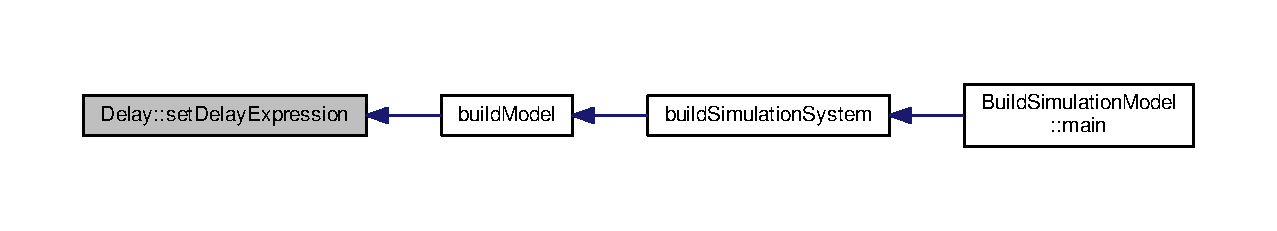
\includegraphics[width=350pt]{class_delay_a683b53af607a424477acb946eb3afdfc_icgraph}
\end{center}
\end{figure}


\hypertarget{class_delay_abe7e89dba0974a81d00e6d2c0548fc1e}{\index{Delay@{Delay}!set\-Delay\-Time\-Unit@{set\-Delay\-Time\-Unit}}
\index{set\-Delay\-Time\-Unit@{set\-Delay\-Time\-Unit}!Delay@{Delay}}
\subsubsection[{set\-Delay\-Time\-Unit}]{\setlength{\rightskip}{0pt plus 5cm}void Delay\-::set\-Delay\-Time\-Unit (
\begin{DoxyParamCaption}
\item[{{\bf Util\-::\-Time\-Unit}}]{\-\_\-delay\-Time\-Unit}
\end{DoxyParamCaption}
)}}\label{class_delay_abe7e89dba0974a81d00e6d2c0548fc1e}


Definition at line 41 of file Delay.\-cpp.

\hypertarget{class_delay_af8187e4515417b547dc22b5ee0a1f95d}{\index{Delay@{Delay}!show@{show}}
\index{show@{show}!Delay@{Delay}}
\subsubsection[{show}]{\setlength{\rightskip}{0pt plus 5cm}std\-::string Delay\-::show (
\begin{DoxyParamCaption}
{}
\end{DoxyParamCaption}
)\hspace{0.3cm}{\ttfamily [virtual]}}}\label{class_delay_af8187e4515417b547dc22b5ee0a1f95d}


Reimplemented from \hyperlink{class_model_component_ad8bc846e36b028eab7efb7da6c549eca}{Model\-Component}.



Definition at line 27 of file Delay.\-cpp.



Here is the call graph for this function\-:\nopagebreak
\begin{figure}[H]
\begin{center}
\leavevmode
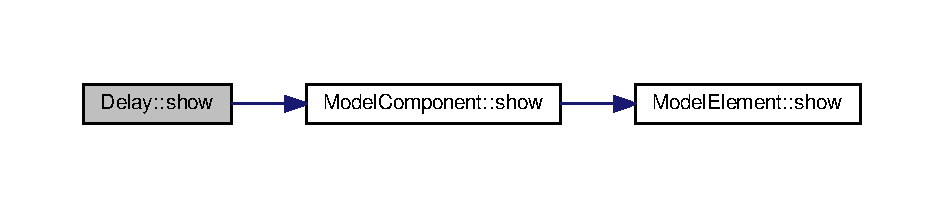
\includegraphics[width=350pt]{class_delay_af8187e4515417b547dc22b5ee0a1f95d_cgraph}
\end{center}
\end{figure}




The documentation for this class was generated from the following files\-:\begin{DoxyCompactItemize}
\item 
\hyperlink{_delay_8h}{Delay.\-h}\item 
\hyperlink{_delay_8cpp}{Delay.\-cpp}\end{DoxyCompactItemize}

\hypertarget{class_dispose}{}\section{Dispose Class Reference}
\label{class_dispose}\index{Dispose@{Dispose}}


{\ttfamily \#include $<$Dispose.\+h$>$}



Inheritance diagram for Dispose\+:
\nopagebreak
\begin{figure}[H]
\begin{center}
\leavevmode
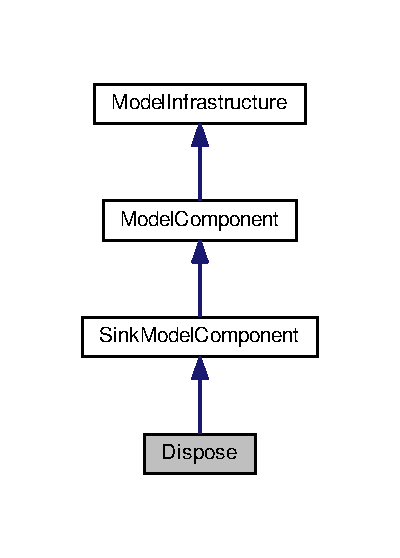
\includegraphics[width=193pt]{class_dispose__inherit__graph}
\end{center}
\end{figure}


Collaboration diagram for Dispose\+:
\nopagebreak
\begin{figure}[H]
\begin{center}
\leavevmode
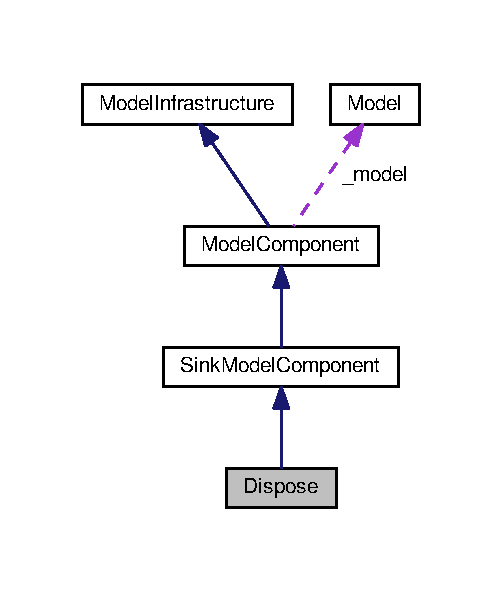
\includegraphics[width=242pt]{class_dispose__coll__graph}
\end{center}
\end{figure}
\subsection*{Public Member Functions}
\begin{DoxyCompactItemize}
\item 
\hyperlink{class_dispose_a9b5ccd61252e7f36d747fd832debdfaa}{Dispose} (\hyperlink{class_model}{Model} $\ast$model)
\item 
\hyperlink{class_dispose_a8d4515962baf1fd7c01912cb654aa683}{Dispose} (const \hyperlink{class_dispose}{Dispose} \&orig)
\item 
virtual \hyperlink{class_dispose_a2a2af23e9cbca66b02a142252a99096d}{$\sim$\+Dispose} ()
\item 
virtual std\+::string \hyperlink{class_dispose_aee8ef98d5ca22eb18a97b258ed059865}{show} ()
\item 
void \hyperlink{class_dispose_a8dc978664e640bc4d58760770b84b84e}{set\+Collect\+Statistics} (bool \+\_\+collect\+Statistics)
\item 
bool \hyperlink{class_dispose_aff15fbea8737b30efe9b3521d12350bd}{is\+Collect\+Statistics} () const 
\end{DoxyCompactItemize}
\subsection*{Protected Member Functions}
\begin{DoxyCompactItemize}
\item 
virtual void \hyperlink{class_dispose_a342eb428496534cdfd17524ad78b0c08}{\+\_\+execute} (\hyperlink{class_entity}{Entity} $\ast$entity)
\item 
virtual void \hyperlink{class_dispose_a245f73bff07925e3efc1eeffd84c9ac6}{\+\_\+load\+Instance} (std\+::list$<$ std\+::string $>$ words)
\item 
virtual std\+::list$<$ std\+::string $>$ $\ast$ \hyperlink{class_dispose_ae12482052fb78fa534dda5d4c0a74e3e}{\+\_\+save\+Instance} ()
\item 
virtual bool \hyperlink{class_dispose_a5ad64b97bbb16662aa9d914eda2a7e38}{\+\_\+verify\+Symbols} (std\+::string $\ast$error\+Message)
\end{DoxyCompactItemize}
\subsection*{Additional Inherited Members}


\subsection{Constructor \& Destructor Documentation}
\index{Dispose@{Dispose}!Dispose@{Dispose}}
\index{Dispose@{Dispose}!Dispose@{Dispose}}
\subsubsection[{\texorpdfstring{Dispose(\+Model $\ast$model)}{Dispose(Model *model)}}]{\setlength{\rightskip}{0pt plus 5cm}Dispose\+::\+Dispose (
\begin{DoxyParamCaption}
\item[{{\bf Model} $\ast$}]{model}
\end{DoxyParamCaption}
)}\hypertarget{class_dispose_a9b5ccd61252e7f36d747fd832debdfaa}{}\label{class_dispose_a9b5ccd61252e7f36d747fd832debdfaa}
\index{Dispose@{Dispose}!Dispose@{Dispose}}
\index{Dispose@{Dispose}!Dispose@{Dispose}}
\subsubsection[{\texorpdfstring{Dispose(const Dispose \&orig)}{Dispose(const Dispose &orig)}}]{\setlength{\rightskip}{0pt plus 5cm}Dispose\+::\+Dispose (
\begin{DoxyParamCaption}
\item[{const {\bf Dispose} \&}]{orig}
\end{DoxyParamCaption}
)}\hypertarget{class_dispose_a8d4515962baf1fd7c01912cb654aa683}{}\label{class_dispose_a8d4515962baf1fd7c01912cb654aa683}
\index{Dispose@{Dispose}!````~Dispose@{$\sim$\+Dispose}}
\index{````~Dispose@{$\sim$\+Dispose}!Dispose@{Dispose}}
\subsubsection[{\texorpdfstring{$\sim$\+Dispose()}{~Dispose()}}]{\setlength{\rightskip}{0pt plus 5cm}Dispose\+::$\sim$\+Dispose (
\begin{DoxyParamCaption}
{}
\end{DoxyParamCaption}
)\hspace{0.3cm}{\ttfamily [virtual]}}\hypertarget{class_dispose_a2a2af23e9cbca66b02a142252a99096d}{}\label{class_dispose_a2a2af23e9cbca66b02a142252a99096d}


\subsection{Member Function Documentation}
\index{Dispose@{Dispose}!\+\_\+execute@{\+\_\+execute}}
\index{\+\_\+execute@{\+\_\+execute}!Dispose@{Dispose}}
\subsubsection[{\texorpdfstring{\+\_\+execute(\+Entity $\ast$entity)}{_execute(Entity *entity)}}]{\setlength{\rightskip}{0pt plus 5cm}void Dispose\+::\+\_\+execute (
\begin{DoxyParamCaption}
\item[{{\bf Entity} $\ast$}]{entity}
\end{DoxyParamCaption}
)\hspace{0.3cm}{\ttfamily [protected]}, {\ttfamily [virtual]}}\hypertarget{class_dispose_a342eb428496534cdfd17524ad78b0c08}{}\label{class_dispose_a342eb428496534cdfd17524ad78b0c08}


Implements \hyperlink{class_model_component_ae3fcf8bbdd8368c882438424aa73f714}{Model\+Component}.

\index{Dispose@{Dispose}!\+\_\+load\+Instance@{\+\_\+load\+Instance}}
\index{\+\_\+load\+Instance@{\+\_\+load\+Instance}!Dispose@{Dispose}}
\subsubsection[{\texorpdfstring{\+\_\+load\+Instance(std\+::list$<$ std\+::string $>$ words)}{_loadInstance(std::list< std::string > words)}}]{\setlength{\rightskip}{0pt plus 5cm}void Dispose\+::\+\_\+load\+Instance (
\begin{DoxyParamCaption}
\item[{std\+::list$<$ std\+::string $>$}]{words}
\end{DoxyParamCaption}
)\hspace{0.3cm}{\ttfamily [protected]}, {\ttfamily [virtual]}}\hypertarget{class_dispose_a245f73bff07925e3efc1eeffd84c9ac6}{}\label{class_dispose_a245f73bff07925e3efc1eeffd84c9ac6}


Implements \hyperlink{class_model_infrastructure_ae118c8ad2ac9d4397c40d004af51b2dc}{Model\+Infrastructure}.

\index{Dispose@{Dispose}!\+\_\+save\+Instance@{\+\_\+save\+Instance}}
\index{\+\_\+save\+Instance@{\+\_\+save\+Instance}!Dispose@{Dispose}}
\subsubsection[{\texorpdfstring{\+\_\+save\+Instance()}{_saveInstance()}}]{\setlength{\rightskip}{0pt plus 5cm}std\+::list$<$ std\+::string $>$ $\ast$ Dispose\+::\+\_\+save\+Instance (
\begin{DoxyParamCaption}
{}
\end{DoxyParamCaption}
)\hspace{0.3cm}{\ttfamily [protected]}, {\ttfamily [virtual]}}\hypertarget{class_dispose_ae12482052fb78fa534dda5d4c0a74e3e}{}\label{class_dispose_ae12482052fb78fa534dda5d4c0a74e3e}


Reimplemented from \hyperlink{class_model_component_a465f41c7191cb0fdf9039ef1f3d755a5}{Model\+Component}.

\index{Dispose@{Dispose}!\+\_\+verify\+Symbols@{\+\_\+verify\+Symbols}}
\index{\+\_\+verify\+Symbols@{\+\_\+verify\+Symbols}!Dispose@{Dispose}}
\subsubsection[{\texorpdfstring{\+\_\+verify\+Symbols(std\+::string $\ast$error\+Message)}{_verifySymbols(std::string *errorMessage)}}]{\setlength{\rightskip}{0pt plus 5cm}bool Dispose\+::\+\_\+verify\+Symbols (
\begin{DoxyParamCaption}
\item[{std\+::string $\ast$}]{error\+Message}
\end{DoxyParamCaption}
)\hspace{0.3cm}{\ttfamily [protected]}, {\ttfamily [virtual]}}\hypertarget{class_dispose_a5ad64b97bbb16662aa9d914eda2a7e38}{}\label{class_dispose_a5ad64b97bbb16662aa9d914eda2a7e38}


Implements \hyperlink{class_model_infrastructure_a43de089b35b96c32dd24ca4f9636a388}{Model\+Infrastructure}.

\index{Dispose@{Dispose}!is\+Collect\+Statistics@{is\+Collect\+Statistics}}
\index{is\+Collect\+Statistics@{is\+Collect\+Statistics}!Dispose@{Dispose}}
\subsubsection[{\texorpdfstring{is\+Collect\+Statistics() const }{isCollectStatistics() const }}]{\setlength{\rightskip}{0pt plus 5cm}bool Dispose\+::is\+Collect\+Statistics (
\begin{DoxyParamCaption}
{}
\end{DoxyParamCaption}
) const}\hypertarget{class_dispose_aff15fbea8737b30efe9b3521d12350bd}{}\label{class_dispose_aff15fbea8737b30efe9b3521d12350bd}
\index{Dispose@{Dispose}!set\+Collect\+Statistics@{set\+Collect\+Statistics}}
\index{set\+Collect\+Statistics@{set\+Collect\+Statistics}!Dispose@{Dispose}}
\subsubsection[{\texorpdfstring{set\+Collect\+Statistics(bool \+\_\+collect\+Statistics)}{setCollectStatistics(bool _collectStatistics)}}]{\setlength{\rightskip}{0pt plus 5cm}void Dispose\+::set\+Collect\+Statistics (
\begin{DoxyParamCaption}
\item[{bool}]{\+\_\+collect\+Statistics}
\end{DoxyParamCaption}
)}\hypertarget{class_dispose_a8dc978664e640bc4d58760770b84b84e}{}\label{class_dispose_a8dc978664e640bc4d58760770b84b84e}
\index{Dispose@{Dispose}!show@{show}}
\index{show@{show}!Dispose@{Dispose}}
\subsubsection[{\texorpdfstring{show()}{show()}}]{\setlength{\rightskip}{0pt plus 5cm}std\+::string Dispose\+::show (
\begin{DoxyParamCaption}
{}
\end{DoxyParamCaption}
)\hspace{0.3cm}{\ttfamily [virtual]}}\hypertarget{class_dispose_aee8ef98d5ca22eb18a97b258ed059865}{}\label{class_dispose_aee8ef98d5ca22eb18a97b258ed059865}


Reimplemented from \hyperlink{class_model_component_ad8bc846e36b028eab7efb7da6c549eca}{Model\+Component}.



The documentation for this class was generated from the following files\+:\begin{DoxyCompactItemize}
\item 
\hyperlink{_dispose_8h}{Dispose.\+h}\item 
\hyperlink{_dispose_8cpp}{Dispose.\+cpp}\end{DoxyCompactItemize}

\hypertarget{class_entity}{\section{Entity Class Reference}
\label{class_entity}\index{Entity@{Entity}}
}


{\ttfamily \#include $<$Entity.\-h$>$}



Inheritance diagram for Entity\-:\nopagebreak
\begin{figure}[H]
\begin{center}
\leavevmode
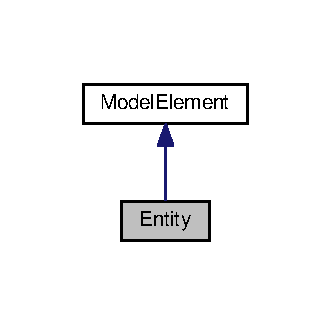
\includegraphics[width=180pt]{class_entity__inherit__graph}
\end{center}
\end{figure}


Collaboration diagram for Entity\-:\nopagebreak
\begin{figure}[H]
\begin{center}
\leavevmode
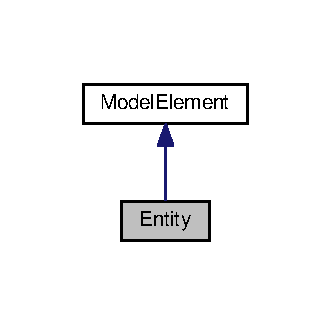
\includegraphics[width=180pt]{class_entity__coll__graph}
\end{center}
\end{figure}
\subsection*{Public Member Functions}
\begin{DoxyCompactItemize}
\item 
\hyperlink{class_entity_a980f368aa07ce358583982821533a54a}{Entity} ()
\item 
\hyperlink{class_entity_a9de139ff12775dd95fb80bec08247de7}{Entity} (const \hyperlink{class_entity}{Entity} \&orig)
\item 
virtual \hyperlink{class_entity_adf6d3f7cb1b2ba029b6b048a395cc8ae}{$\sim$\-Entity} ()
\item 
virtual std\-::string \hyperlink{class_entity_a86cc324050b451b31b134943e7978e36}{show} ()
\item 
std\-::map$<$ std\-::string, \\*
\hyperlink{class_attribute_value}{Attribute\-Value} $\ast$ $>$ $\ast$ \hyperlink{class_entity_a5990dbefc2f21a7e8e0f91f9bf434fb9}{get\-Attribute\-Values} () const 
\item 
void \hyperlink{class_entity_a40053760a2c84dd72fd5aeb425f6781d}{set\-Entity\-Type\-Name} (std\-::string \-\_\-entity\-Type\-Name)
\item 
std\-::string \hyperlink{class_entity_a860a6385aa2af6b8d205a8e3ea912c38}{get\-Entity\-Type\-Name} () const 
\end{DoxyCompactItemize}
\subsection*{Additional Inherited Members}


\subsection{Constructor \& Destructor Documentation}
\hypertarget{class_entity_a980f368aa07ce358583982821533a54a}{\index{Entity@{Entity}!Entity@{Entity}}
\index{Entity@{Entity}!Entity@{Entity}}
\subsubsection[{Entity}]{\setlength{\rightskip}{0pt plus 5cm}Entity\-::\-Entity (
\begin{DoxyParamCaption}
{}
\end{DoxyParamCaption}
)}}\label{class_entity_a980f368aa07ce358583982821533a54a}
\hypertarget{class_entity_a9de139ff12775dd95fb80bec08247de7}{\index{Entity@{Entity}!Entity@{Entity}}
\index{Entity@{Entity}!Entity@{Entity}}
\subsubsection[{Entity}]{\setlength{\rightskip}{0pt plus 5cm}Entity\-::\-Entity (
\begin{DoxyParamCaption}
\item[{const {\bf Entity} \&}]{orig}
\end{DoxyParamCaption}
)}}\label{class_entity_a9de139ff12775dd95fb80bec08247de7}
\hypertarget{class_entity_adf6d3f7cb1b2ba029b6b048a395cc8ae}{\index{Entity@{Entity}!$\sim$\-Entity@{$\sim$\-Entity}}
\index{$\sim$\-Entity@{$\sim$\-Entity}!Entity@{Entity}}
\subsubsection[{$\sim$\-Entity}]{\setlength{\rightskip}{0pt plus 5cm}Entity\-::$\sim$\-Entity (
\begin{DoxyParamCaption}
{}
\end{DoxyParamCaption}
)\hspace{0.3cm}{\ttfamily [virtual]}}}\label{class_entity_adf6d3f7cb1b2ba029b6b048a395cc8ae}


\subsection{Member Function Documentation}
\hypertarget{class_entity_a5990dbefc2f21a7e8e0f91f9bf434fb9}{\index{Entity@{Entity}!get\-Attribute\-Values@{get\-Attribute\-Values}}
\index{get\-Attribute\-Values@{get\-Attribute\-Values}!Entity@{Entity}}
\subsubsection[{get\-Attribute\-Values}]{\setlength{\rightskip}{0pt plus 5cm}std\-::map$<$ std\-::string, {\bf Attribute\-Value} $\ast$ $>$ $\ast$ Entity\-::get\-Attribute\-Values (
\begin{DoxyParamCaption}
{}
\end{DoxyParamCaption}
) const}}\label{class_entity_a5990dbefc2f21a7e8e0f91f9bf434fb9}
\hypertarget{class_entity_a860a6385aa2af6b8d205a8e3ea912c38}{\index{Entity@{Entity}!get\-Entity\-Type\-Name@{get\-Entity\-Type\-Name}}
\index{get\-Entity\-Type\-Name@{get\-Entity\-Type\-Name}!Entity@{Entity}}
\subsubsection[{get\-Entity\-Type\-Name}]{\setlength{\rightskip}{0pt plus 5cm}std\-::string Entity\-::get\-Entity\-Type\-Name (
\begin{DoxyParamCaption}
{}
\end{DoxyParamCaption}
) const}}\label{class_entity_a860a6385aa2af6b8d205a8e3ea912c38}
\hypertarget{class_entity_a40053760a2c84dd72fd5aeb425f6781d}{\index{Entity@{Entity}!set\-Entity\-Type\-Name@{set\-Entity\-Type\-Name}}
\index{set\-Entity\-Type\-Name@{set\-Entity\-Type\-Name}!Entity@{Entity}}
\subsubsection[{set\-Entity\-Type\-Name}]{\setlength{\rightskip}{0pt plus 5cm}void Entity\-::set\-Entity\-Type\-Name (
\begin{DoxyParamCaption}
\item[{std\-::string}]{\-\_\-entity\-Type\-Name}
\end{DoxyParamCaption}
)}}\label{class_entity_a40053760a2c84dd72fd5aeb425f6781d}
\hypertarget{class_entity_a86cc324050b451b31b134943e7978e36}{\index{Entity@{Entity}!show@{show}}
\index{show@{show}!Entity@{Entity}}
\subsubsection[{show}]{\setlength{\rightskip}{0pt plus 5cm}std\-::string Entity\-::show (
\begin{DoxyParamCaption}
{}
\end{DoxyParamCaption}
)\hspace{0.3cm}{\ttfamily [virtual]}}}\label{class_entity_a86cc324050b451b31b134943e7978e36}


Reimplemented from \hyperlink{class_model_infrastructure_a649a5a89a0c9931783d3c51de2acf266}{Model\-Infrastructure}.



Here is the call graph for this function\-:\nopagebreak
\begin{figure}[H]
\begin{center}
\leavevmode
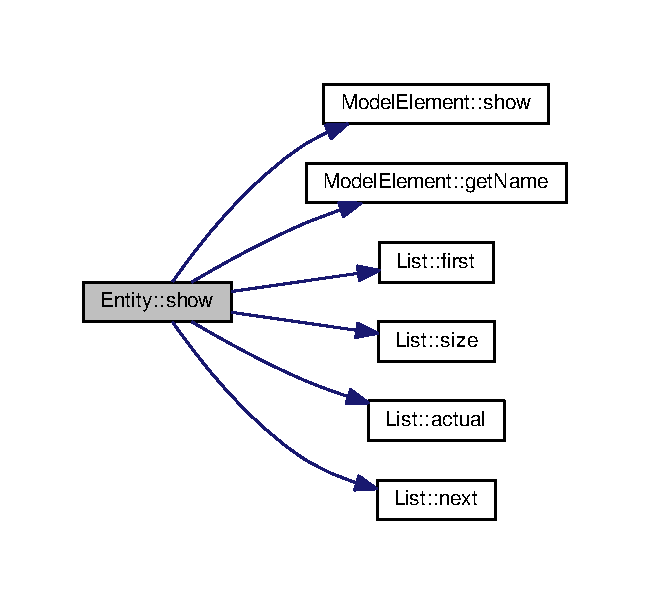
\includegraphics[width=290pt]{class_entity_a86cc324050b451b31b134943e7978e36_cgraph}
\end{center}
\end{figure}




The documentation for this class was generated from the following files\-:\begin{DoxyCompactItemize}
\item 
\hyperlink{_entity_8h}{Entity.\-h}\item 
\hyperlink{_entity_8cpp}{Entity.\-cpp}\end{DoxyCompactItemize}

\hypertarget{class_entity_type}{\section{Entity\-Type Class Reference}
\label{class_entity_type}\index{Entity\-Type@{Entity\-Type}}
}


{\ttfamily \#include $<$Entity\-Type.\-h$>$}



Inheritance diagram for Entity\-Type\-:\nopagebreak
\begin{figure}[H]
\begin{center}
\leavevmode
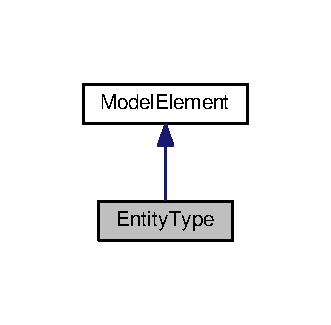
\includegraphics[width=180pt]{class_entity_type__inherit__graph}
\end{center}
\end{figure}


Collaboration diagram for Entity\-Type\-:\nopagebreak
\begin{figure}[H]
\begin{center}
\leavevmode
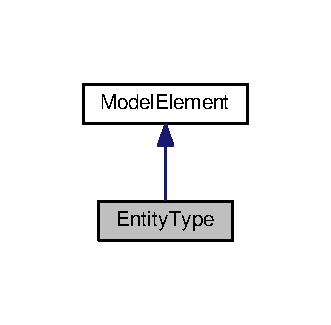
\includegraphics[width=180pt]{class_entity_type__coll__graph}
\end{center}
\end{figure}
\subsection*{Public Member Functions}
\begin{DoxyCompactItemize}
\item 
\hyperlink{class_entity_type_a76c09c732793a586dc3b474485e9824f}{Entity\-Type} (\hyperlink{class_model}{Model} $\ast$model)
\item 
\hyperlink{class_entity_type_a34b9576e2453ed309c75840319bbb2f8}{Entity\-Type} (const \hyperlink{class_entity_type}{Entity\-Type} \&orig)
\item 
virtual \hyperlink{class_entity_type_aee11e4242d000965f06018723bdf0946}{$\sim$\-Entity\-Type} ()
\item 
virtual std\-::string \hyperlink{class_entity_type_ab5a696912b12a9f51decded90f368dea}{show} ()
\item 
void \hyperlink{class_entity_type_affd1d2dd13149ae0989aae5cc9ea1e05}{set\-Initial\-Waiting\-Cost} (double \-\_\-initial\-Waiting\-Cost)
\item 
double \hyperlink{class_entity_type_a46dd0977b19bf167eeb12db97464b757}{get\-Initial\-Waiting\-Cost} () const 
\item 
void \hyperlink{class_entity_type_a32f126822c567a887a446a763db13d64}{set\-Initial\-Other\-Cost} (double \-\_\-initial\-Other\-Cost)
\item 
double \hyperlink{class_entity_type_ac5708811f5f6eaf7ac587fc88190b7f2}{get\-Initial\-Other\-Cost} () const 
\item 
void \hyperlink{class_entity_type_a935cac67adc2b13aa25290c3db04c847}{set\-Initial\-N\-V\-A\-Cost} (double \-\_\-initial\-N\-V\-A\-Cost)
\item 
double \hyperlink{class_entity_type_ae8b26deba82e687d5a07b863f750baf4}{get\-Initial\-N\-V\-A\-Cost} () const 
\item 
void \hyperlink{class_entity_type_aecd52de7178bb03be55798378d15d3e8}{set\-Initial\-V\-A\-Cost} (double \-\_\-initial\-V\-A\-Cost)
\item 
double \hyperlink{class_entity_type_a9833d4a85dcb5c5bd9db02e1e2e45dd9}{get\-Initial\-V\-A\-Cost} () const 
\item 
void \hyperlink{class_entity_type_ab3a19031f9b46b376bdd35aa3044c90e}{set\-Initial\-Picture} (std\-::string \-\_\-initial\-Picture)
\item 
std\-::string \hyperlink{class_entity_type_a9a464c546bc2f7fe56fbea9b761ac1f7}{get\-Initial\-Picture} () const 
\item 
\hyperlink{class_statistics_collector}{Statistics\-Collector} $\ast$ \hyperlink{class_entity_type_acdcb00168a8fc2e23cf8bf3302464ce3}{get\-Cstat\-Time\-In\-System} () const 
\item 
\hyperlink{class_statistics_collector}{Statistics\-Collector} $\ast$ \hyperlink{class_entity_type_a48e1dedd3e7d7b198ee4e7a61c6afb7e}{get\-Cstat\-N\-V\-A\-Time} () const 
\item 
\hyperlink{class_statistics_collector}{Statistics\-Collector} $\ast$ \hyperlink{class_entity_type_aafb65d3cdceae776da454989b7b4a874}{get\-Cstat\-V\-A\-Time} () const 
\item 
\hyperlink{class_statistics_collector}{Statistics\-Collector} $\ast$ \hyperlink{class_entity_type_a8b6a8b11d428c9e23800d01701e7fbd1}{get\-Cstat\-Other\-Time} () const 
\item 
\hyperlink{class_statistics_collector}{Statistics\-Collector} $\ast$ \hyperlink{class_entity_type_a2604288226dd7fc0c6c322d415b891cc}{get\-Cstat\-Transfer\-Time} () const 
\item 
\hyperlink{class_statistics_collector}{Statistics\-Collector} $\ast$ \hyperlink{class_entity_type_ae43feed54cd8661efb317ef4891bcfcf}{get\-Cstat\-Waiting\-Time} () const 
\end{DoxyCompactItemize}
\subsection*{Protected Member Functions}
\begin{DoxyCompactItemize}
\item 
virtual void \hyperlink{class_entity_type_af88c3d67f9eb8b92b4e32e04bed6730f}{\-\_\-load\-Instance} (std\-::list$<$ std\-::string $>$ words)
\item 
virtual std\-::list$<$ std\-::string $>$ $\ast$ \hyperlink{class_entity_type_a4f6179d5043e750d9555d6eeef8de4cd}{\-\_\-save\-Instance} ()
\item 
virtual bool \hyperlink{class_entity_type_a50e21c4807823132e777529c70bf7cef}{\-\_\-verify\-Symbols} (std\-::string $\ast$error\-Message)
\end{DoxyCompactItemize}
\subsection*{Additional Inherited Members}


\subsection{Detailed Description}


Definition at line 22 of file Entity\-Type.\-h.



\subsection{Constructor \& Destructor Documentation}
\hypertarget{class_entity_type_a76c09c732793a586dc3b474485e9824f}{\index{Entity\-Type@{Entity\-Type}!Entity\-Type@{Entity\-Type}}
\index{Entity\-Type@{Entity\-Type}!EntityType@{Entity\-Type}}
\subsubsection[{Entity\-Type}]{\setlength{\rightskip}{0pt plus 5cm}Entity\-Type\-::\-Entity\-Type (
\begin{DoxyParamCaption}
\item[{{\bf Model} $\ast$}]{model}
\end{DoxyParamCaption}
)}}\label{class_entity_type_a76c09c732793a586dc3b474485e9824f}


Definition at line 18 of file Entity\-Type.\-cpp.



Here is the call graph for this function\-:
\nopagebreak
\begin{figure}[H]
\begin{center}
\leavevmode
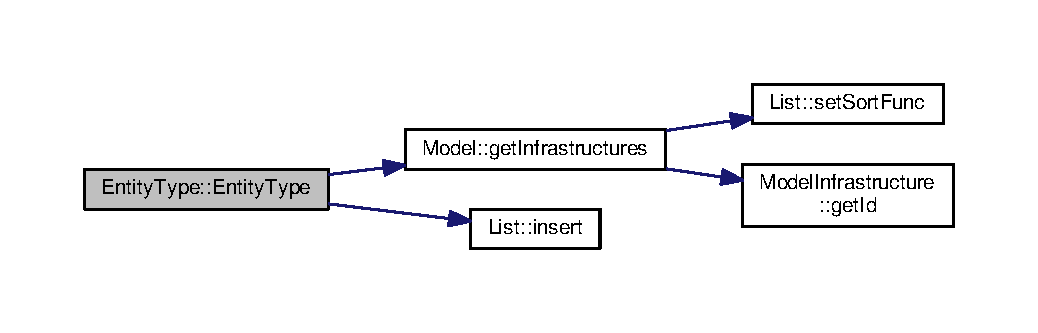
\includegraphics[width=350pt]{class_entity_type_a76c09c732793a586dc3b474485e9824f_cgraph}
\end{center}
\end{figure}


\hypertarget{class_entity_type_a34b9576e2453ed309c75840319bbb2f8}{\index{Entity\-Type@{Entity\-Type}!Entity\-Type@{Entity\-Type}}
\index{Entity\-Type@{Entity\-Type}!EntityType@{Entity\-Type}}
\subsubsection[{Entity\-Type}]{\setlength{\rightskip}{0pt plus 5cm}Entity\-Type\-::\-Entity\-Type (
\begin{DoxyParamCaption}
\item[{const {\bf Entity\-Type} \&}]{orig}
\end{DoxyParamCaption}
)}}\label{class_entity_type_a34b9576e2453ed309c75840319bbb2f8}


Definition at line 29 of file Entity\-Type.\-cpp.

\hypertarget{class_entity_type_aee11e4242d000965f06018723bdf0946}{\index{Entity\-Type@{Entity\-Type}!$\sim$\-Entity\-Type@{$\sim$\-Entity\-Type}}
\index{$\sim$\-Entity\-Type@{$\sim$\-Entity\-Type}!EntityType@{Entity\-Type}}
\subsubsection[{$\sim$\-Entity\-Type}]{\setlength{\rightskip}{0pt plus 5cm}Entity\-Type\-::$\sim$\-Entity\-Type (
\begin{DoxyParamCaption}
{}
\end{DoxyParamCaption}
)\hspace{0.3cm}{\ttfamily [virtual]}}}\label{class_entity_type_aee11e4242d000965f06018723bdf0946}


Definition at line 32 of file Entity\-Type.\-cpp.



\subsection{Member Function Documentation}
\hypertarget{class_entity_type_af88c3d67f9eb8b92b4e32e04bed6730f}{\index{Entity\-Type@{Entity\-Type}!\-\_\-load\-Instance@{\-\_\-load\-Instance}}
\index{\-\_\-load\-Instance@{\-\_\-load\-Instance}!EntityType@{Entity\-Type}}
\subsubsection[{\-\_\-load\-Instance}]{\setlength{\rightskip}{0pt plus 5cm}void Entity\-Type\-::\-\_\-load\-Instance (
\begin{DoxyParamCaption}
\item[{std\-::list$<$ std\-::string $>$}]{words}
\end{DoxyParamCaption}
)\hspace{0.3cm}{\ttfamily [protected]}, {\ttfamily [virtual]}}}\label{class_entity_type_af88c3d67f9eb8b92b4e32e04bed6730f}


Implements \hyperlink{class_model_infrastructure_ae118c8ad2ac9d4397c40d004af51b2dc}{Model\-Infrastructure}.



Definition at line 104 of file Entity\-Type.\-cpp.

\hypertarget{class_entity_type_a4f6179d5043e750d9555d6eeef8de4cd}{\index{Entity\-Type@{Entity\-Type}!\-\_\-save\-Instance@{\-\_\-save\-Instance}}
\index{\-\_\-save\-Instance@{\-\_\-save\-Instance}!EntityType@{Entity\-Type}}
\subsubsection[{\-\_\-save\-Instance}]{\setlength{\rightskip}{0pt plus 5cm}std\-::list$<$ std\-::string $>$ $\ast$ Entity\-Type\-::\-\_\-save\-Instance (
\begin{DoxyParamCaption}
{}
\end{DoxyParamCaption}
)\hspace{0.3cm}{\ttfamily [protected]}, {\ttfamily [virtual]}}}\label{class_entity_type_a4f6179d5043e750d9555d6eeef8de4cd}


Implements \hyperlink{class_model_infrastructure_a3da2fd381c44752598bc448b207e8287}{Model\-Infrastructure}.



Definition at line 108 of file Entity\-Type.\-cpp.

\hypertarget{class_entity_type_a50e21c4807823132e777529c70bf7cef}{\index{Entity\-Type@{Entity\-Type}!\-\_\-verify\-Symbols@{\-\_\-verify\-Symbols}}
\index{\-\_\-verify\-Symbols@{\-\_\-verify\-Symbols}!EntityType@{Entity\-Type}}
\subsubsection[{\-\_\-verify\-Symbols}]{\setlength{\rightskip}{0pt plus 5cm}bool Entity\-Type\-::\-\_\-verify\-Symbols (
\begin{DoxyParamCaption}
\item[{std\-::string $\ast$}]{error\-Message}
\end{DoxyParamCaption}
)\hspace{0.3cm}{\ttfamily [protected]}, {\ttfamily [virtual]}}}\label{class_entity_type_a50e21c4807823132e777529c70bf7cef}


Implements \hyperlink{class_model_infrastructure_a43de089b35b96c32dd24ca4f9636a388}{Model\-Infrastructure}.



Definition at line 113 of file Entity\-Type.\-cpp.

\hypertarget{class_entity_type_a48e1dedd3e7d7b198ee4e7a61c6afb7e}{\index{Entity\-Type@{Entity\-Type}!get\-Cstat\-N\-V\-A\-Time@{get\-Cstat\-N\-V\-A\-Time}}
\index{get\-Cstat\-N\-V\-A\-Time@{get\-Cstat\-N\-V\-A\-Time}!EntityType@{Entity\-Type}}
\subsubsection[{get\-Cstat\-N\-V\-A\-Time}]{\setlength{\rightskip}{0pt plus 5cm}{\bf Statistics\-Collector} $\ast$ Entity\-Type\-::get\-Cstat\-N\-V\-A\-Time (
\begin{DoxyParamCaption}
{}
\end{DoxyParamCaption}
) const}}\label{class_entity_type_a48e1dedd3e7d7b198ee4e7a61c6afb7e}


Definition at line 84 of file Entity\-Type.\-cpp.

\hypertarget{class_entity_type_a8b6a8b11d428c9e23800d01701e7fbd1}{\index{Entity\-Type@{Entity\-Type}!get\-Cstat\-Other\-Time@{get\-Cstat\-Other\-Time}}
\index{get\-Cstat\-Other\-Time@{get\-Cstat\-Other\-Time}!EntityType@{Entity\-Type}}
\subsubsection[{get\-Cstat\-Other\-Time}]{\setlength{\rightskip}{0pt plus 5cm}{\bf Statistics\-Collector} $\ast$ Entity\-Type\-::get\-Cstat\-Other\-Time (
\begin{DoxyParamCaption}
{}
\end{DoxyParamCaption}
) const}}\label{class_entity_type_a8b6a8b11d428c9e23800d01701e7fbd1}


Definition at line 92 of file Entity\-Type.\-cpp.

\hypertarget{class_entity_type_acdcb00168a8fc2e23cf8bf3302464ce3}{\index{Entity\-Type@{Entity\-Type}!get\-Cstat\-Time\-In\-System@{get\-Cstat\-Time\-In\-System}}
\index{get\-Cstat\-Time\-In\-System@{get\-Cstat\-Time\-In\-System}!EntityType@{Entity\-Type}}
\subsubsection[{get\-Cstat\-Time\-In\-System}]{\setlength{\rightskip}{0pt plus 5cm}{\bf Statistics\-Collector} $\ast$ Entity\-Type\-::get\-Cstat\-Time\-In\-System (
\begin{DoxyParamCaption}
{}
\end{DoxyParamCaption}
) const}}\label{class_entity_type_acdcb00168a8fc2e23cf8bf3302464ce3}


Definition at line 80 of file Entity\-Type.\-cpp.

\hypertarget{class_entity_type_a2604288226dd7fc0c6c322d415b891cc}{\index{Entity\-Type@{Entity\-Type}!get\-Cstat\-Transfer\-Time@{get\-Cstat\-Transfer\-Time}}
\index{get\-Cstat\-Transfer\-Time@{get\-Cstat\-Transfer\-Time}!EntityType@{Entity\-Type}}
\subsubsection[{get\-Cstat\-Transfer\-Time}]{\setlength{\rightskip}{0pt plus 5cm}{\bf Statistics\-Collector} $\ast$ Entity\-Type\-::get\-Cstat\-Transfer\-Time (
\begin{DoxyParamCaption}
{}
\end{DoxyParamCaption}
) const}}\label{class_entity_type_a2604288226dd7fc0c6c322d415b891cc}


Definition at line 96 of file Entity\-Type.\-cpp.

\hypertarget{class_entity_type_aafb65d3cdceae776da454989b7b4a874}{\index{Entity\-Type@{Entity\-Type}!get\-Cstat\-V\-A\-Time@{get\-Cstat\-V\-A\-Time}}
\index{get\-Cstat\-V\-A\-Time@{get\-Cstat\-V\-A\-Time}!EntityType@{Entity\-Type}}
\subsubsection[{get\-Cstat\-V\-A\-Time}]{\setlength{\rightskip}{0pt plus 5cm}{\bf Statistics\-Collector} $\ast$ Entity\-Type\-::get\-Cstat\-V\-A\-Time (
\begin{DoxyParamCaption}
{}
\end{DoxyParamCaption}
) const}}\label{class_entity_type_aafb65d3cdceae776da454989b7b4a874}


Definition at line 88 of file Entity\-Type.\-cpp.

\hypertarget{class_entity_type_ae43feed54cd8661efb317ef4891bcfcf}{\index{Entity\-Type@{Entity\-Type}!get\-Cstat\-Waiting\-Time@{get\-Cstat\-Waiting\-Time}}
\index{get\-Cstat\-Waiting\-Time@{get\-Cstat\-Waiting\-Time}!EntityType@{Entity\-Type}}
\subsubsection[{get\-Cstat\-Waiting\-Time}]{\setlength{\rightskip}{0pt plus 5cm}{\bf Statistics\-Collector} $\ast$ Entity\-Type\-::get\-Cstat\-Waiting\-Time (
\begin{DoxyParamCaption}
{}
\end{DoxyParamCaption}
) const}}\label{class_entity_type_ae43feed54cd8661efb317ef4891bcfcf}


Definition at line 100 of file Entity\-Type.\-cpp.

\hypertarget{class_entity_type_ae8b26deba82e687d5a07b863f750baf4}{\index{Entity\-Type@{Entity\-Type}!get\-Initial\-N\-V\-A\-Cost@{get\-Initial\-N\-V\-A\-Cost}}
\index{get\-Initial\-N\-V\-A\-Cost@{get\-Initial\-N\-V\-A\-Cost}!EntityType@{Entity\-Type}}
\subsubsection[{get\-Initial\-N\-V\-A\-Cost}]{\setlength{\rightskip}{0pt plus 5cm}double Entity\-Type\-::get\-Initial\-N\-V\-A\-Cost (
\begin{DoxyParamCaption}
{}
\end{DoxyParamCaption}
) const}}\label{class_entity_type_ae8b26deba82e687d5a07b863f750baf4}


Definition at line 60 of file Entity\-Type.\-cpp.

\hypertarget{class_entity_type_ac5708811f5f6eaf7ac587fc88190b7f2}{\index{Entity\-Type@{Entity\-Type}!get\-Initial\-Other\-Cost@{get\-Initial\-Other\-Cost}}
\index{get\-Initial\-Other\-Cost@{get\-Initial\-Other\-Cost}!EntityType@{Entity\-Type}}
\subsubsection[{get\-Initial\-Other\-Cost}]{\setlength{\rightskip}{0pt plus 5cm}double Entity\-Type\-::get\-Initial\-Other\-Cost (
\begin{DoxyParamCaption}
{}
\end{DoxyParamCaption}
) const}}\label{class_entity_type_ac5708811f5f6eaf7ac587fc88190b7f2}


Definition at line 52 of file Entity\-Type.\-cpp.

\hypertarget{class_entity_type_a9a464c546bc2f7fe56fbea9b761ac1f7}{\index{Entity\-Type@{Entity\-Type}!get\-Initial\-Picture@{get\-Initial\-Picture}}
\index{get\-Initial\-Picture@{get\-Initial\-Picture}!EntityType@{Entity\-Type}}
\subsubsection[{get\-Initial\-Picture}]{\setlength{\rightskip}{0pt plus 5cm}std\-::string Entity\-Type\-::get\-Initial\-Picture (
\begin{DoxyParamCaption}
{}
\end{DoxyParamCaption}
) const}}\label{class_entity_type_a9a464c546bc2f7fe56fbea9b761ac1f7}


Definition at line 76 of file Entity\-Type.\-cpp.

\hypertarget{class_entity_type_a9833d4a85dcb5c5bd9db02e1e2e45dd9}{\index{Entity\-Type@{Entity\-Type}!get\-Initial\-V\-A\-Cost@{get\-Initial\-V\-A\-Cost}}
\index{get\-Initial\-V\-A\-Cost@{get\-Initial\-V\-A\-Cost}!EntityType@{Entity\-Type}}
\subsubsection[{get\-Initial\-V\-A\-Cost}]{\setlength{\rightskip}{0pt plus 5cm}double Entity\-Type\-::get\-Initial\-V\-A\-Cost (
\begin{DoxyParamCaption}
{}
\end{DoxyParamCaption}
) const}}\label{class_entity_type_a9833d4a85dcb5c5bd9db02e1e2e45dd9}


Definition at line 68 of file Entity\-Type.\-cpp.

\hypertarget{class_entity_type_a46dd0977b19bf167eeb12db97464b757}{\index{Entity\-Type@{Entity\-Type}!get\-Initial\-Waiting\-Cost@{get\-Initial\-Waiting\-Cost}}
\index{get\-Initial\-Waiting\-Cost@{get\-Initial\-Waiting\-Cost}!EntityType@{Entity\-Type}}
\subsubsection[{get\-Initial\-Waiting\-Cost}]{\setlength{\rightskip}{0pt plus 5cm}double Entity\-Type\-::get\-Initial\-Waiting\-Cost (
\begin{DoxyParamCaption}
{}
\end{DoxyParamCaption}
) const}}\label{class_entity_type_a46dd0977b19bf167eeb12db97464b757}


Definition at line 44 of file Entity\-Type.\-cpp.

\hypertarget{class_entity_type_a935cac67adc2b13aa25290c3db04c847}{\index{Entity\-Type@{Entity\-Type}!set\-Initial\-N\-V\-A\-Cost@{set\-Initial\-N\-V\-A\-Cost}}
\index{set\-Initial\-N\-V\-A\-Cost@{set\-Initial\-N\-V\-A\-Cost}!EntityType@{Entity\-Type}}
\subsubsection[{set\-Initial\-N\-V\-A\-Cost}]{\setlength{\rightskip}{0pt plus 5cm}void Entity\-Type\-::set\-Initial\-N\-V\-A\-Cost (
\begin{DoxyParamCaption}
\item[{double}]{\-\_\-initial\-N\-V\-A\-Cost}
\end{DoxyParamCaption}
)}}\label{class_entity_type_a935cac67adc2b13aa25290c3db04c847}


Definition at line 56 of file Entity\-Type.\-cpp.

\hypertarget{class_entity_type_a32f126822c567a887a446a763db13d64}{\index{Entity\-Type@{Entity\-Type}!set\-Initial\-Other\-Cost@{set\-Initial\-Other\-Cost}}
\index{set\-Initial\-Other\-Cost@{set\-Initial\-Other\-Cost}!EntityType@{Entity\-Type}}
\subsubsection[{set\-Initial\-Other\-Cost}]{\setlength{\rightskip}{0pt plus 5cm}void Entity\-Type\-::set\-Initial\-Other\-Cost (
\begin{DoxyParamCaption}
\item[{double}]{\-\_\-initial\-Other\-Cost}
\end{DoxyParamCaption}
)}}\label{class_entity_type_a32f126822c567a887a446a763db13d64}


Definition at line 48 of file Entity\-Type.\-cpp.

\hypertarget{class_entity_type_ab3a19031f9b46b376bdd35aa3044c90e}{\index{Entity\-Type@{Entity\-Type}!set\-Initial\-Picture@{set\-Initial\-Picture}}
\index{set\-Initial\-Picture@{set\-Initial\-Picture}!EntityType@{Entity\-Type}}
\subsubsection[{set\-Initial\-Picture}]{\setlength{\rightskip}{0pt plus 5cm}void Entity\-Type\-::set\-Initial\-Picture (
\begin{DoxyParamCaption}
\item[{std\-::string}]{\-\_\-initial\-Picture}
\end{DoxyParamCaption}
)}}\label{class_entity_type_ab3a19031f9b46b376bdd35aa3044c90e}


Definition at line 72 of file Entity\-Type.\-cpp.

\hypertarget{class_entity_type_aecd52de7178bb03be55798378d15d3e8}{\index{Entity\-Type@{Entity\-Type}!set\-Initial\-V\-A\-Cost@{set\-Initial\-V\-A\-Cost}}
\index{set\-Initial\-V\-A\-Cost@{set\-Initial\-V\-A\-Cost}!EntityType@{Entity\-Type}}
\subsubsection[{set\-Initial\-V\-A\-Cost}]{\setlength{\rightskip}{0pt plus 5cm}void Entity\-Type\-::set\-Initial\-V\-A\-Cost (
\begin{DoxyParamCaption}
\item[{double}]{\-\_\-initial\-V\-A\-Cost}
\end{DoxyParamCaption}
)}}\label{class_entity_type_aecd52de7178bb03be55798378d15d3e8}


Definition at line 64 of file Entity\-Type.\-cpp.

\hypertarget{class_entity_type_affd1d2dd13149ae0989aae5cc9ea1e05}{\index{Entity\-Type@{Entity\-Type}!set\-Initial\-Waiting\-Cost@{set\-Initial\-Waiting\-Cost}}
\index{set\-Initial\-Waiting\-Cost@{set\-Initial\-Waiting\-Cost}!EntityType@{Entity\-Type}}
\subsubsection[{set\-Initial\-Waiting\-Cost}]{\setlength{\rightskip}{0pt plus 5cm}void Entity\-Type\-::set\-Initial\-Waiting\-Cost (
\begin{DoxyParamCaption}
\item[{double}]{\-\_\-initial\-Waiting\-Cost}
\end{DoxyParamCaption}
)}}\label{class_entity_type_affd1d2dd13149ae0989aae5cc9ea1e05}


Definition at line 40 of file Entity\-Type.\-cpp.

\hypertarget{class_entity_type_ab5a696912b12a9f51decded90f368dea}{\index{Entity\-Type@{Entity\-Type}!show@{show}}
\index{show@{show}!EntityType@{Entity\-Type}}
\subsubsection[{show}]{\setlength{\rightskip}{0pt plus 5cm}std\-::string Entity\-Type\-::show (
\begin{DoxyParamCaption}
{}
\end{DoxyParamCaption}
)\hspace{0.3cm}{\ttfamily [virtual]}}}\label{class_entity_type_ab5a696912b12a9f51decded90f368dea}


Reimplemented from \hyperlink{class_model_infrastructure_a649a5a89a0c9931783d3c51de2acf266}{Model\-Infrastructure}.



Definition at line 35 of file Entity\-Type.\-cpp.



Here is the call graph for this function\-:\nopagebreak
\begin{figure}[H]
\begin{center}
\leavevmode
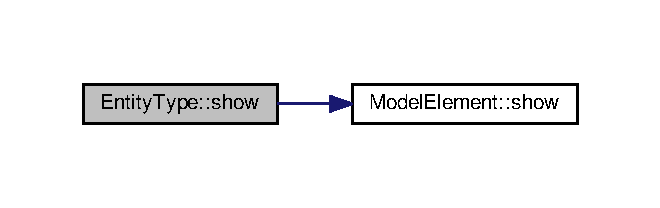
\includegraphics[width=312pt]{class_entity_type_ab5a696912b12a9f51decded90f368dea_cgraph}
\end{center}
\end{figure}




The documentation for this class was generated from the following files\-:\begin{DoxyCompactItemize}
\item 
\hyperlink{_entity_type_8h}{Entity\-Type.\-h}\item 
\hyperlink{_entity_type_8cpp}{Entity\-Type.\-cpp}\end{DoxyCompactItemize}

\hypertarget{class_event}{\section{Event Class Reference}
\label{class_event}\index{Event@{Event}}
}


{\ttfamily \#include $<$Event.\-h$>$}

\subsection*{Public Member Functions}
\begin{DoxyCompactItemize}
\item 
\hyperlink{class_event_a81e573f9452ca3a4d1b07e2347235e87}{Event} (double time, \hyperlink{class_entity}{Entity} $\ast$entity, \hyperlink{class_model_component}{Model\-Component} $\ast$component)
\item 
\hyperlink{class_event_a537ad58d679329069468e8cf2b2904d0}{Event} (const \hyperlink{class_event}{Event} \&orig)
\item 
virtual \hyperlink{class_event_a7704ec01ce91e673885792054214b3d2}{$\sim$\-Event} ()
\item 
double \hyperlink{class_event_a008a7989d0849a45613917cedc27f27e}{get\-Time} () const 
\item 
\hyperlink{class_model_component}{Model\-Component} $\ast$ \hyperlink{class_event_a7fb897ded1b3f0b946b25740f2e2eda0}{get\-Component} () const 
\item 
\hyperlink{class_entity}{Entity} $\ast$ \hyperlink{class_event_a6890c776c6c2e13abbc0892fc7333102}{get\-Entity} () const 
\item 
std\-::string \hyperlink{class_event_a640f132001d454af52cb0d0e20ebb856}{show} ()
\end{DoxyCompactItemize}


\subsection{Detailed Description}


Definition at line 22 of file Event.\-h.



\subsection{Constructor \& Destructor Documentation}
\hypertarget{class_event_a81e573f9452ca3a4d1b07e2347235e87}{\index{Event@{Event}!Event@{Event}}
\index{Event@{Event}!Event@{Event}}
\subsubsection[{Event}]{\setlength{\rightskip}{0pt plus 5cm}Event\-::\-Event (
\begin{DoxyParamCaption}
\item[{double}]{time, }
\item[{{\bf Entity} $\ast$}]{entity, }
\item[{{\bf Model\-Component} $\ast$}]{component}
\end{DoxyParamCaption}
)}}\label{class_event_a81e573f9452ca3a4d1b07e2347235e87}


Definition at line 16 of file Event.\-cpp.

\hypertarget{class_event_a537ad58d679329069468e8cf2b2904d0}{\index{Event@{Event}!Event@{Event}}
\index{Event@{Event}!Event@{Event}}
\subsubsection[{Event}]{\setlength{\rightskip}{0pt plus 5cm}Event\-::\-Event (
\begin{DoxyParamCaption}
\item[{const {\bf Event} \&}]{orig}
\end{DoxyParamCaption}
)}}\label{class_event_a537ad58d679329069468e8cf2b2904d0}


Definition at line 22 of file Event.\-cpp.

\hypertarget{class_event_a7704ec01ce91e673885792054214b3d2}{\index{Event@{Event}!$\sim$\-Event@{$\sim$\-Event}}
\index{$\sim$\-Event@{$\sim$\-Event}!Event@{Event}}
\subsubsection[{$\sim$\-Event}]{\setlength{\rightskip}{0pt plus 5cm}Event\-::$\sim$\-Event (
\begin{DoxyParamCaption}
{}
\end{DoxyParamCaption}
)\hspace{0.3cm}{\ttfamily [virtual]}}}\label{class_event_a7704ec01ce91e673885792054214b3d2}


Definition at line 25 of file Event.\-cpp.



\subsection{Member Function Documentation}
\hypertarget{class_event_a7fb897ded1b3f0b946b25740f2e2eda0}{\index{Event@{Event}!get\-Component@{get\-Component}}
\index{get\-Component@{get\-Component}!Event@{Event}}
\subsubsection[{get\-Component}]{\setlength{\rightskip}{0pt plus 5cm}{\bf Model\-Component} $\ast$ Event\-::get\-Component (
\begin{DoxyParamCaption}
{}
\end{DoxyParamCaption}
) const}}\label{class_event_a7fb897ded1b3f0b946b25740f2e2eda0}


Definition at line 38 of file Event.\-cpp.

\hypertarget{class_event_a6890c776c6c2e13abbc0892fc7333102}{\index{Event@{Event}!get\-Entity@{get\-Entity}}
\index{get\-Entity@{get\-Entity}!Event@{Event}}
\subsubsection[{get\-Entity}]{\setlength{\rightskip}{0pt plus 5cm}{\bf Entity} $\ast$ Event\-::get\-Entity (
\begin{DoxyParamCaption}
{}
\end{DoxyParamCaption}
) const}}\label{class_event_a6890c776c6c2e13abbc0892fc7333102}


Definition at line 42 of file Event.\-cpp.

\hypertarget{class_event_a008a7989d0849a45613917cedc27f27e}{\index{Event@{Event}!get\-Time@{get\-Time}}
\index{get\-Time@{get\-Time}!Event@{Event}}
\subsubsection[{get\-Time}]{\setlength{\rightskip}{0pt plus 5cm}double Event\-::get\-Time (
\begin{DoxyParamCaption}
{}
\end{DoxyParamCaption}
) const}}\label{class_event_a008a7989d0849a45613917cedc27f27e}


Definition at line 34 of file Event.\-cpp.



Here is the caller graph for this function\-:
\nopagebreak
\begin{figure}[H]
\begin{center}
\leavevmode
\includegraphics[width=282pt]{class_event_a008a7989d0849a45613917cedc27f27e_icgraph}
\end{center}
\end{figure}


\hypertarget{class_event_a640f132001d454af52cb0d0e20ebb856}{\index{Event@{Event}!show@{show}}
\index{show@{show}!Event@{Event}}
\subsubsection[{show}]{\setlength{\rightskip}{0pt plus 5cm}std\-::string Event\-::show (
\begin{DoxyParamCaption}
{}
\end{DoxyParamCaption}
)}}\label{class_event_a640f132001d454af52cb0d0e20ebb856}


Definition at line 28 of file Event.\-cpp.



Here is the call graph for this function\-:\nopagebreak
\begin{figure}[H]
\begin{center}
\leavevmode
\includegraphics[width=290pt]{class_event_a640f132001d454af52cb0d0e20ebb856_cgraph}
\end{center}
\end{figure}




The documentation for this class was generated from the following files\-:\begin{DoxyCompactItemize}
\item 
\hyperlink{_event_8h}{Event.\-h}\item 
\hyperlink{_event_8cpp}{Event.\-cpp}\end{DoxyCompactItemize}

\hypertarget{class_experiment_design__if}{\section{Experiment\-Design\-\_\-if Class Reference}
\label{class_experiment_design__if}\index{Experiment\-Design\-\_\-if@{Experiment\-Design\-\_\-if}}
}


{\ttfamily \#include $<$Experiment\-Design\-\_\-if.\-h$>$}



Inheritance diagram for Experiment\-Design\-\_\-if\-:
\nopagebreak
\begin{figure}[H]
\begin{center}
\leavevmode
\includegraphics[width=214pt]{class_experiment_design__if__inherit__graph}
\end{center}
\end{figure}
\subsection*{Public Member Functions}
\begin{DoxyCompactItemize}
\item 
virtual \hyperlink{class_process_analyser__if}{Process\-Analyser\-\_\-if} $\ast$ \hyperlink{class_experiment_design__if_ad3d35aef077b45d683e408ee756d83aa}{get\-Process\-Analyser} () const =0
\item 
virtual bool \hyperlink{class_experiment_design__if_a590a79e47f10294ed9d806baa9a98cba}{generate2kr\-Scenario\-Experiments} ()=0
\item 
virtual bool \hyperlink{class_experiment_design__if_a5e8a8698eaf74121671dd007d7a000e9}{calculate\-Contribution\-And\-Coefficients} ()=0
\item 
virtual std\-::list\\*
$<$ \hyperlink{class_factor_or_interaction_contribution}{Factor\-Or\-Interaction\-Contribution} $\ast$ $>$ $\ast$ \hyperlink{class_experiment_design__if_a249bd184b8326ec6e161321fe6fb7dbe}{get\-Contributions} () const =0
\end{DoxyCompactItemize}


\subsection{Detailed Description}
It designs a set of experiments (\hyperlink{class_simulation_scenario}{Simulation\-Scenario}) where que level of factors (\hyperlink{class_simulation_control}{Simulation\-Control}) are set automatically to create a 2$^\wedge$k.r experiment design, and where the contributions of the factors and their interactions (just a set of \hyperlink{class_simulation_control}{Simulation\-Control}) can be obtained. 

Definition at line 23 of file Experiment\-Design\-\_\-if.\-h.



\subsection{Member Function Documentation}
\hypertarget{class_experiment_design__if_a5e8a8698eaf74121671dd007d7a000e9}{\index{Experiment\-Design\-\_\-if@{Experiment\-Design\-\_\-if}!calculate\-Contribution\-And\-Coefficients@{calculate\-Contribution\-And\-Coefficients}}
\index{calculate\-Contribution\-And\-Coefficients@{calculate\-Contribution\-And\-Coefficients}!ExperimentDesign_if@{Experiment\-Design\-\_\-if}}
\subsubsection[{calculate\-Contribution\-And\-Coefficients}]{\setlength{\rightskip}{0pt plus 5cm}virtual bool Experiment\-Design\-\_\-if\-::calculate\-Contribution\-And\-Coefficients (
\begin{DoxyParamCaption}
{}
\end{DoxyParamCaption}
)\hspace{0.3cm}{\ttfamily [pure virtual]}}}\label{class_experiment_design__if_a5e8a8698eaf74121671dd007d7a000e9}


Implemented in \hyperlink{class_experiment_design_my_impl1_ad6da633ae27de1e860b012f53f1b4c7a}{Experiment\-Design\-My\-Impl1}.

\hypertarget{class_experiment_design__if_a590a79e47f10294ed9d806baa9a98cba}{\index{Experiment\-Design\-\_\-if@{Experiment\-Design\-\_\-if}!generate2kr\-Scenario\-Experiments@{generate2kr\-Scenario\-Experiments}}
\index{generate2kr\-Scenario\-Experiments@{generate2kr\-Scenario\-Experiments}!ExperimentDesign_if@{Experiment\-Design\-\_\-if}}
\subsubsection[{generate2kr\-Scenario\-Experiments}]{\setlength{\rightskip}{0pt plus 5cm}virtual bool Experiment\-Design\-\_\-if\-::generate2kr\-Scenario\-Experiments (
\begin{DoxyParamCaption}
{}
\end{DoxyParamCaption}
)\hspace{0.3cm}{\ttfamily [pure virtual]}}}\label{class_experiment_design__if_a590a79e47f10294ed9d806baa9a98cba}


Implemented in \hyperlink{class_experiment_design_my_impl1_a8f7417fa4fd5ba274e8b734238f18e4b}{Experiment\-Design\-My\-Impl1}.

\hypertarget{class_experiment_design__if_a249bd184b8326ec6e161321fe6fb7dbe}{\index{Experiment\-Design\-\_\-if@{Experiment\-Design\-\_\-if}!get\-Contributions@{get\-Contributions}}
\index{get\-Contributions@{get\-Contributions}!ExperimentDesign_if@{Experiment\-Design\-\_\-if}}
\subsubsection[{get\-Contributions}]{\setlength{\rightskip}{0pt plus 5cm}virtual std\-::list$<${\bf Factor\-Or\-Interaction\-Contribution}$\ast$$>$$\ast$ Experiment\-Design\-\_\-if\-::get\-Contributions (
\begin{DoxyParamCaption}
{}
\end{DoxyParamCaption}
) const\hspace{0.3cm}{\ttfamily [pure virtual]}}}\label{class_experiment_design__if_a249bd184b8326ec6e161321fe6fb7dbe}


Implemented in \hyperlink{class_experiment_design_my_impl1_ab75393cb5f481243618dc3687e930cd2}{Experiment\-Design\-My\-Impl1}.

\hypertarget{class_experiment_design__if_ad3d35aef077b45d683e408ee756d83aa}{\index{Experiment\-Design\-\_\-if@{Experiment\-Design\-\_\-if}!get\-Process\-Analyser@{get\-Process\-Analyser}}
\index{get\-Process\-Analyser@{get\-Process\-Analyser}!ExperimentDesign_if@{Experiment\-Design\-\_\-if}}
\subsubsection[{get\-Process\-Analyser}]{\setlength{\rightskip}{0pt plus 5cm}virtual {\bf Process\-Analyser\-\_\-if}$\ast$ Experiment\-Design\-\_\-if\-::get\-Process\-Analyser (
\begin{DoxyParamCaption}
{}
\end{DoxyParamCaption}
) const\hspace{0.3cm}{\ttfamily [pure virtual]}}}\label{class_experiment_design__if_ad3d35aef077b45d683e408ee756d83aa}


Implemented in \hyperlink{class_experiment_design_my_impl1_a776e79e146621df6b6966b2e1e99ffc0}{Experiment\-Design\-My\-Impl1}.



The documentation for this class was generated from the following file\-:\begin{DoxyCompactItemize}
\item 
\hyperlink{_experiment_design__if_8h}{Experiment\-Design\-\_\-if.\-h}\end{DoxyCompactItemize}

\hypertarget{class_experiment_design_my_impl1}{\section{Experiment\-Design\-My\-Impl1 Class Reference}
\label{class_experiment_design_my_impl1}\index{Experiment\-Design\-My\-Impl1@{Experiment\-Design\-My\-Impl1}}
}


{\ttfamily \#include $<$Experiment\-Design\-My\-Impl1.\-h$>$}



Inheritance diagram for Experiment\-Design\-My\-Impl1\-:\nopagebreak
\begin{figure}[H]
\begin{center}
\leavevmode
\includegraphics[width=214pt]{class_experiment_design_my_impl1__inherit__graph}
\end{center}
\end{figure}


Collaboration diagram for Experiment\-Design\-My\-Impl1\-:\nopagebreak
\begin{figure}[H]
\begin{center}
\leavevmode
\includegraphics[width=214pt]{class_experiment_design_my_impl1__coll__graph}
\end{center}
\end{figure}
\subsection*{Public Member Functions}
\begin{DoxyCompactItemize}
\item 
\hyperlink{class_experiment_design_my_impl1_acc95e63ecb8987b816e58a73aa7ee64b}{Experiment\-Design\-My\-Impl1} ()
\item 
\hyperlink{class_experiment_design_my_impl1_a8acecbd450fbb0d7d22a5fee8341d865}{Experiment\-Design\-My\-Impl1} (const \hyperlink{class_experiment_design_my_impl1}{Experiment\-Design\-My\-Impl1} \&orig)
\item 
virtual \hyperlink{class_experiment_design_my_impl1_ae9effad5f7e3d88023b470daae6616a2}{$\sim$\-Experiment\-Design\-My\-Impl1} ()
\item 
\hyperlink{class_process_analyser__if}{Process\-Analyser\-\_\-if} $\ast$ \hyperlink{class_experiment_design_my_impl1_a776e79e146621df6b6966b2e1e99ffc0}{get\-Process\-Analyser} () const 
\item 
bool \hyperlink{class_experiment_design_my_impl1_a8f7417fa4fd5ba274e8b734238f18e4b}{generate2kr\-Scenario\-Experiments} ()
\item 
bool \hyperlink{class_experiment_design_my_impl1_ad6da633ae27de1e860b012f53f1b4c7a}{calculate\-Contribution\-And\-Coefficients} ()
\item 
std\-::list\\*
$<$ \hyperlink{class_factor_or_interaction_contribution}{Factor\-Or\-Interaction\-Contribution} $\ast$ $>$ $\ast$ \hyperlink{class_experiment_design_my_impl1_ab75393cb5f481243618dc3687e930cd2}{get\-Contributions} () const 
\end{DoxyCompactItemize}


\subsection{Detailed Description}


Definition at line 22 of file Experiment\-Design\-My\-Impl1.\-h.



\subsection{Constructor \& Destructor Documentation}
\hypertarget{class_experiment_design_my_impl1_acc95e63ecb8987b816e58a73aa7ee64b}{\index{Experiment\-Design\-My\-Impl1@{Experiment\-Design\-My\-Impl1}!Experiment\-Design\-My\-Impl1@{Experiment\-Design\-My\-Impl1}}
\index{Experiment\-Design\-My\-Impl1@{Experiment\-Design\-My\-Impl1}!ExperimentDesignMyImpl1@{Experiment\-Design\-My\-Impl1}}
\subsubsection[{Experiment\-Design\-My\-Impl1}]{\setlength{\rightskip}{0pt plus 5cm}Experiment\-Design\-My\-Impl1\-::\-Experiment\-Design\-My\-Impl1 (
\begin{DoxyParamCaption}
{}
\end{DoxyParamCaption}
)}}\label{class_experiment_design_my_impl1_acc95e63ecb8987b816e58a73aa7ee64b}


Definition at line 17 of file Experiment\-Design\-My\-Impl1.\-cpp.

\hypertarget{class_experiment_design_my_impl1_a8acecbd450fbb0d7d22a5fee8341d865}{\index{Experiment\-Design\-My\-Impl1@{Experiment\-Design\-My\-Impl1}!Experiment\-Design\-My\-Impl1@{Experiment\-Design\-My\-Impl1}}
\index{Experiment\-Design\-My\-Impl1@{Experiment\-Design\-My\-Impl1}!ExperimentDesignMyImpl1@{Experiment\-Design\-My\-Impl1}}
\subsubsection[{Experiment\-Design\-My\-Impl1}]{\setlength{\rightskip}{0pt plus 5cm}Experiment\-Design\-My\-Impl1\-::\-Experiment\-Design\-My\-Impl1 (
\begin{DoxyParamCaption}
\item[{const {\bf Experiment\-Design\-My\-Impl1} \&}]{orig}
\end{DoxyParamCaption}
)}}\label{class_experiment_design_my_impl1_a8acecbd450fbb0d7d22a5fee8341d865}


Definition at line 24 of file Experiment\-Design\-My\-Impl1.\-cpp.

\hypertarget{class_experiment_design_my_impl1_ae9effad5f7e3d88023b470daae6616a2}{\index{Experiment\-Design\-My\-Impl1@{Experiment\-Design\-My\-Impl1}!$\sim$\-Experiment\-Design\-My\-Impl1@{$\sim$\-Experiment\-Design\-My\-Impl1}}
\index{$\sim$\-Experiment\-Design\-My\-Impl1@{$\sim$\-Experiment\-Design\-My\-Impl1}!ExperimentDesignMyImpl1@{Experiment\-Design\-My\-Impl1}}
\subsubsection[{$\sim$\-Experiment\-Design\-My\-Impl1}]{\setlength{\rightskip}{0pt plus 5cm}Experiment\-Design\-My\-Impl1\-::$\sim$\-Experiment\-Design\-My\-Impl1 (
\begin{DoxyParamCaption}
{}
\end{DoxyParamCaption}
)\hspace{0.3cm}{\ttfamily [virtual]}}}\label{class_experiment_design_my_impl1_ae9effad5f7e3d88023b470daae6616a2}


Definition at line 27 of file Experiment\-Design\-My\-Impl1.\-cpp.



\subsection{Member Function Documentation}
\hypertarget{class_experiment_design_my_impl1_ad6da633ae27de1e860b012f53f1b4c7a}{\index{Experiment\-Design\-My\-Impl1@{Experiment\-Design\-My\-Impl1}!calculate\-Contribution\-And\-Coefficients@{calculate\-Contribution\-And\-Coefficients}}
\index{calculate\-Contribution\-And\-Coefficients@{calculate\-Contribution\-And\-Coefficients}!ExperimentDesignMyImpl1@{Experiment\-Design\-My\-Impl1}}
\subsubsection[{calculate\-Contribution\-And\-Coefficients}]{\setlength{\rightskip}{0pt plus 5cm}bool Experiment\-Design\-My\-Impl1\-::calculate\-Contribution\-And\-Coefficients (
\begin{DoxyParamCaption}
{}
\end{DoxyParamCaption}
)\hspace{0.3cm}{\ttfamily [virtual]}}}\label{class_experiment_design_my_impl1_ad6da633ae27de1e860b012f53f1b4c7a}


Implements \hyperlink{class_experiment_design__if_a5e8a8698eaf74121671dd007d7a000e9}{Experiment\-Design\-\_\-if}.



Definition at line 34 of file Experiment\-Design\-My\-Impl1.\-cpp.

\hypertarget{class_experiment_design_my_impl1_a8f7417fa4fd5ba274e8b734238f18e4b}{\index{Experiment\-Design\-My\-Impl1@{Experiment\-Design\-My\-Impl1}!generate2kr\-Scenario\-Experiments@{generate2kr\-Scenario\-Experiments}}
\index{generate2kr\-Scenario\-Experiments@{generate2kr\-Scenario\-Experiments}!ExperimentDesignMyImpl1@{Experiment\-Design\-My\-Impl1}}
\subsubsection[{generate2kr\-Scenario\-Experiments}]{\setlength{\rightskip}{0pt plus 5cm}bool Experiment\-Design\-My\-Impl1\-::generate2kr\-Scenario\-Experiments (
\begin{DoxyParamCaption}
{}
\end{DoxyParamCaption}
)\hspace{0.3cm}{\ttfamily [virtual]}}}\label{class_experiment_design_my_impl1_a8f7417fa4fd5ba274e8b734238f18e4b}


Implements \hyperlink{class_experiment_design__if_a590a79e47f10294ed9d806baa9a98cba}{Experiment\-Design\-\_\-if}.



Definition at line 30 of file Experiment\-Design\-My\-Impl1.\-cpp.

\hypertarget{class_experiment_design_my_impl1_ab75393cb5f481243618dc3687e930cd2}{\index{Experiment\-Design\-My\-Impl1@{Experiment\-Design\-My\-Impl1}!get\-Contributions@{get\-Contributions}}
\index{get\-Contributions@{get\-Contributions}!ExperimentDesignMyImpl1@{Experiment\-Design\-My\-Impl1}}
\subsubsection[{get\-Contributions}]{\setlength{\rightskip}{0pt plus 5cm}std\-::list$<$ {\bf Factor\-Or\-Interaction\-Contribution} $\ast$ $>$ $\ast$ Experiment\-Design\-My\-Impl1\-::get\-Contributions (
\begin{DoxyParamCaption}
{}
\end{DoxyParamCaption}
) const\hspace{0.3cm}{\ttfamily [virtual]}}}\label{class_experiment_design_my_impl1_ab75393cb5f481243618dc3687e930cd2}


Implements \hyperlink{class_experiment_design__if_a249bd184b8326ec6e161321fe6fb7dbe}{Experiment\-Design\-\_\-if}.



Definition at line 20 of file Experiment\-Design\-My\-Impl1.\-cpp.

\hypertarget{class_experiment_design_my_impl1_a776e79e146621df6b6966b2e1e99ffc0}{\index{Experiment\-Design\-My\-Impl1@{Experiment\-Design\-My\-Impl1}!get\-Process\-Analyser@{get\-Process\-Analyser}}
\index{get\-Process\-Analyser@{get\-Process\-Analyser}!ExperimentDesignMyImpl1@{Experiment\-Design\-My\-Impl1}}
\subsubsection[{get\-Process\-Analyser}]{\setlength{\rightskip}{0pt plus 5cm}{\bf Process\-Analyser\-\_\-if} $\ast$ Experiment\-Design\-My\-Impl1\-::get\-Process\-Analyser (
\begin{DoxyParamCaption}
{}
\end{DoxyParamCaption}
) const\hspace{0.3cm}{\ttfamily [virtual]}}}\label{class_experiment_design_my_impl1_a776e79e146621df6b6966b2e1e99ffc0}


Implements \hyperlink{class_experiment_design__if_ad3d35aef077b45d683e408ee756d83aa}{Experiment\-Design\-\_\-if}.



Definition at line 38 of file Experiment\-Design\-My\-Impl1.\-cpp.



The documentation for this class was generated from the following files\-:\begin{DoxyCompactItemize}
\item 
\hyperlink{_experiment_design_my_impl1_8h}{Experiment\-Design\-My\-Impl1.\-h}\item 
\hyperlink{_experiment_design_my_impl1_8cpp}{Experiment\-Design\-My\-Impl1.\-cpp}\end{DoxyCompactItemize}

\hypertarget{class_factor_or_interaction_contribution}{\section{Factor\-Or\-Interaction\-Contribution Class Reference}
\label{class_factor_or_interaction_contribution}\index{Factor\-Or\-Interaction\-Contribution@{Factor\-Or\-Interaction\-Contribution}}
}


{\ttfamily \#include $<$Factor\-Or\-Interaction\-Contribution.\-h$>$}

\subsection*{Public Member Functions}
\begin{DoxyCompactItemize}
\item 
\hyperlink{class_factor_or_interaction_contribution_aee33d23a9255292a4c9e7bb7c1b02e2d}{Factor\-Or\-Interaction\-Contribution} (double contribution, double model\-Coefficient, std\-::list$<$ \hyperlink{class_simulation_control}{Simulation\-Control} $\ast$ $>$ $\ast$controls)
\item 
\hyperlink{class_factor_or_interaction_contribution_a6c3335e47b137605f7258ceb6233be3a}{Factor\-Or\-Interaction\-Contribution} (const \hyperlink{class_factor_or_interaction_contribution}{Factor\-Or\-Interaction\-Contribution} \&orig)
\item 
\hyperlink{class_factor_or_interaction_contribution_ae9efdcdc1f162a045fc7b4bff3abf7b7}{$\sim$\-Factor\-Or\-Interaction\-Contribution} ()
\item 
double \hyperlink{class_factor_or_interaction_contribution_af1d9b3083c6176a1ac96f6abfa476c3c}{get\-Model\-Coefficient} () const 
\item 
std\-::list$<$ \hyperlink{class_simulation_control}{Simulation\-Control} $\ast$ $>$ $\ast$ \hyperlink{class_factor_or_interaction_contribution_a12556ece8eb1b2e9c31186571cabfea4}{get\-Controls} () const 
\item 
double \hyperlink{class_factor_or_interaction_contribution_ad0113b8462ffdf1040fe43f5f4f25e4a}{get\-Contribution} () const 
\end{DoxyCompactItemize}


\subsection{Detailed Description}
This simple class corresponds to a factor when it refers to just one \hyperlink{class_simulation_control}{Simulation\-Control}, or to the interaction between two or more factors when it refers to more \hyperlink{class_simulation_control}{Simulation\-Control}. It also encapsulates the contribution of the factor or interaction and its coefficient in the full model that estimates one specific \hyperlink{class_simulation_response}{Simulation\-Response}. 

Definition at line 23 of file Factor\-Or\-Interaction\-Contribution.\-h.



\subsection{Constructor \& Destructor Documentation}
\hypertarget{class_factor_or_interaction_contribution_aee33d23a9255292a4c9e7bb7c1b02e2d}{\index{Factor\-Or\-Interaction\-Contribution@{Factor\-Or\-Interaction\-Contribution}!Factor\-Or\-Interaction\-Contribution@{Factor\-Or\-Interaction\-Contribution}}
\index{Factor\-Or\-Interaction\-Contribution@{Factor\-Or\-Interaction\-Contribution}!FactorOrInteractionContribution@{Factor\-Or\-Interaction\-Contribution}}
\subsubsection[{Factor\-Or\-Interaction\-Contribution}]{\setlength{\rightskip}{0pt plus 5cm}Factor\-Or\-Interaction\-Contribution\-::\-Factor\-Or\-Interaction\-Contribution (
\begin{DoxyParamCaption}
\item[{double}]{contribution, }
\item[{double}]{model\-Coefficient, }
\item[{std\-::list$<$ {\bf Simulation\-Control} $\ast$ $>$ $\ast$}]{controls}
\end{DoxyParamCaption}
)}}\label{class_factor_or_interaction_contribution_aee33d23a9255292a4c9e7bb7c1b02e2d}


Definition at line 17 of file Factor\-Or\-Interaction\-Contribution.\-cpp.

\hypertarget{class_factor_or_interaction_contribution_a6c3335e47b137605f7258ceb6233be3a}{\index{Factor\-Or\-Interaction\-Contribution@{Factor\-Or\-Interaction\-Contribution}!Factor\-Or\-Interaction\-Contribution@{Factor\-Or\-Interaction\-Contribution}}
\index{Factor\-Or\-Interaction\-Contribution@{Factor\-Or\-Interaction\-Contribution}!FactorOrInteractionContribution@{Factor\-Or\-Interaction\-Contribution}}
\subsubsection[{Factor\-Or\-Interaction\-Contribution}]{\setlength{\rightskip}{0pt plus 5cm}Factor\-Or\-Interaction\-Contribution\-::\-Factor\-Or\-Interaction\-Contribution (
\begin{DoxyParamCaption}
\item[{const {\bf Factor\-Or\-Interaction\-Contribution} \&}]{orig}
\end{DoxyParamCaption}
)}}\label{class_factor_or_interaction_contribution_a6c3335e47b137605f7258ceb6233be3a}


Definition at line 23 of file Factor\-Or\-Interaction\-Contribution.\-cpp.

\hypertarget{class_factor_or_interaction_contribution_ae9efdcdc1f162a045fc7b4bff3abf7b7}{\index{Factor\-Or\-Interaction\-Contribution@{Factor\-Or\-Interaction\-Contribution}!$\sim$\-Factor\-Or\-Interaction\-Contribution@{$\sim$\-Factor\-Or\-Interaction\-Contribution}}
\index{$\sim$\-Factor\-Or\-Interaction\-Contribution@{$\sim$\-Factor\-Or\-Interaction\-Contribution}!FactorOrInteractionContribution@{Factor\-Or\-Interaction\-Contribution}}
\subsubsection[{$\sim$\-Factor\-Or\-Interaction\-Contribution}]{\setlength{\rightskip}{0pt plus 5cm}Factor\-Or\-Interaction\-Contribution\-::$\sim$\-Factor\-Or\-Interaction\-Contribution (
\begin{DoxyParamCaption}
{}
\end{DoxyParamCaption}
)}}\label{class_factor_or_interaction_contribution_ae9efdcdc1f162a045fc7b4bff3abf7b7}


Definition at line 26 of file Factor\-Or\-Interaction\-Contribution.\-cpp.



\subsection{Member Function Documentation}
\hypertarget{class_factor_or_interaction_contribution_ad0113b8462ffdf1040fe43f5f4f25e4a}{\index{Factor\-Or\-Interaction\-Contribution@{Factor\-Or\-Interaction\-Contribution}!get\-Contribution@{get\-Contribution}}
\index{get\-Contribution@{get\-Contribution}!FactorOrInteractionContribution@{Factor\-Or\-Interaction\-Contribution}}
\subsubsection[{get\-Contribution}]{\setlength{\rightskip}{0pt plus 5cm}double Factor\-Or\-Interaction\-Contribution\-::get\-Contribution (
\begin{DoxyParamCaption}
{}
\end{DoxyParamCaption}
) const}}\label{class_factor_or_interaction_contribution_ad0113b8462ffdf1040fe43f5f4f25e4a}


Definition at line 37 of file Factor\-Or\-Interaction\-Contribution.\-cpp.

\hypertarget{class_factor_or_interaction_contribution_a12556ece8eb1b2e9c31186571cabfea4}{\index{Factor\-Or\-Interaction\-Contribution@{Factor\-Or\-Interaction\-Contribution}!get\-Controls@{get\-Controls}}
\index{get\-Controls@{get\-Controls}!FactorOrInteractionContribution@{Factor\-Or\-Interaction\-Contribution}}
\subsubsection[{get\-Controls}]{\setlength{\rightskip}{0pt plus 5cm}std\-::list$<$ {\bf Simulation\-Control} $\ast$ $>$ $\ast$ Factor\-Or\-Interaction\-Contribution\-::get\-Controls (
\begin{DoxyParamCaption}
{}
\end{DoxyParamCaption}
) const}}\label{class_factor_or_interaction_contribution_a12556ece8eb1b2e9c31186571cabfea4}


Definition at line 33 of file Factor\-Or\-Interaction\-Contribution.\-cpp.

\hypertarget{class_factor_or_interaction_contribution_af1d9b3083c6176a1ac96f6abfa476c3c}{\index{Factor\-Or\-Interaction\-Contribution@{Factor\-Or\-Interaction\-Contribution}!get\-Model\-Coefficient@{get\-Model\-Coefficient}}
\index{get\-Model\-Coefficient@{get\-Model\-Coefficient}!FactorOrInteractionContribution@{Factor\-Or\-Interaction\-Contribution}}
\subsubsection[{get\-Model\-Coefficient}]{\setlength{\rightskip}{0pt plus 5cm}double Factor\-Or\-Interaction\-Contribution\-::get\-Model\-Coefficient (
\begin{DoxyParamCaption}
{}
\end{DoxyParamCaption}
) const}}\label{class_factor_or_interaction_contribution_af1d9b3083c6176a1ac96f6abfa476c3c}


Definition at line 29 of file Factor\-Or\-Interaction\-Contribution.\-cpp.



The documentation for this class was generated from the following files\-:\begin{DoxyCompactItemize}
\item 
\hyperlink{_factor_or_interaction_contribution_8h}{Factor\-Or\-Interaction\-Contribution.\-h}\item 
\hyperlink{_factor_or_interaction_contribution_8cpp}{Factor\-Or\-Interaction\-Contribution.\-cpp}\end{DoxyCompactItemize}

\hypertarget{class_fitter__if}{\section{Fitter\-\_\-if Class Reference}
\label{class_fitter__if}\index{Fitter\-\_\-if@{Fitter\-\_\-if}}
}


{\ttfamily \#include $<$Fitter\-\_\-if.\-h$>$}



Inheritance diagram for Fitter\-\_\-if\-:\nopagebreak
\begin{figure}[H]
\begin{center}
\leavevmode
\includegraphics[width=156pt]{class_fitter__if__inherit__graph}
\end{center}
\end{figure}
\subsection*{Public Member Functions}
\begin{DoxyCompactItemize}
\item 
virtual bool \hyperlink{class_fitter__if_a53e98635fcdee314e8ade8089f41ddad}{is\-Normal\-Distributed} (double confidencelevel)=0
\item 
virtual void \hyperlink{class_fitter__if_adec53dfede4bdb31b175e57e6a2c2fc7}{fit\-Uniform} (double $\ast$sqrerror, double $\ast$min, double $\ast$max)=0
\item 
virtual void \hyperlink{class_fitter__if_a2bfc41c6a8044520aeafb2c5c71fe570}{fit\-Triangular} (double $\ast$sqrerror, double $\ast$min, double $\ast$mo, double $\ast$max)=0
\item 
virtual void \hyperlink{class_fitter__if_af95b4de00b7ed5d67b10d9ee458379bf}{fit\-Normal} (double $\ast$sqrerror, double $\ast$avg, double $\ast$stddev)=0
\item 
virtual void \hyperlink{class_fitter__if_a5ab5ac575b736bb720e6a40b334de5a3}{fit\-Expo} (double $\ast$sqrerror, double $\ast$avg1)=0
\item 
virtual void \hyperlink{class_fitter__if_aa46a5cd2d50d3cab34a719099e1058a1}{fit\-Erlang} (double $\ast$sqrerror, double $\ast$a, double $\ast$b, double $\ast$offset, double $\ast$mult)=0
\item 
virtual void \hyperlink{class_fitter__if_a686a7d540919b2e604df93b3049562d1}{fit\-Beta} (double $\ast$sqrerror, double $\ast$a, double $\ast$b, double $\ast$offset, double $\ast$mult)=0
\item 
virtual void \hyperlink{class_fitter__if_ae46e4cbb4354d6d06167aa498855d7ea}{fit\-Weibull} (double $\ast$sqrerror, double $\ast$a, double $\ast$b, double $\ast$offset, double $\ast$mult)=0
\item 
virtual void \hyperlink{class_fitter__if_a819a5ca8715ba4be30d2c7a3957aa467}{fit\-All} (double $\ast$sqrerror, std\-::string $\ast$name)=0
\item 
virtual void \hyperlink{class_fitter__if_aa2d2f13548a09a2f727a4190a6b9c2dd}{set\-Data\-Filename} (std\-::string data\-Filename)=0
\item 
virtual std\-::string \hyperlink{class_fitter__if_a3c6926020b1224a960890fe308abcc86}{get\-Data\-Filename} ()=0
\end{DoxyCompactItemize}


\subsection{Member Function Documentation}
\hypertarget{class_fitter__if_a819a5ca8715ba4be30d2c7a3957aa467}{\index{Fitter\-\_\-if@{Fitter\-\_\-if}!fit\-All@{fit\-All}}
\index{fit\-All@{fit\-All}!Fitter_if@{Fitter\-\_\-if}}
\subsubsection[{fit\-All}]{\setlength{\rightskip}{0pt plus 5cm}virtual void Fitter\-\_\-if\-::fit\-All (
\begin{DoxyParamCaption}
\item[{double $\ast$}]{sqrerror, }
\item[{std\-::string $\ast$}]{name}
\end{DoxyParamCaption}
)\hspace{0.3cm}{\ttfamily [pure virtual]}}}\label{class_fitter__if_a819a5ca8715ba4be30d2c7a3957aa467}


Implemented in \hyperlink{class_fitter_my_impl1_ad10f9269396cb86f2230edf652242f23}{Fitter\-My\-Impl1}.

\hypertarget{class_fitter__if_a686a7d540919b2e604df93b3049562d1}{\index{Fitter\-\_\-if@{Fitter\-\_\-if}!fit\-Beta@{fit\-Beta}}
\index{fit\-Beta@{fit\-Beta}!Fitter_if@{Fitter\-\_\-if}}
\subsubsection[{fit\-Beta}]{\setlength{\rightskip}{0pt plus 5cm}virtual void Fitter\-\_\-if\-::fit\-Beta (
\begin{DoxyParamCaption}
\item[{double $\ast$}]{sqrerror, }
\item[{double $\ast$}]{a, }
\item[{double $\ast$}]{b, }
\item[{double $\ast$}]{offset, }
\item[{double $\ast$}]{mult}
\end{DoxyParamCaption}
)\hspace{0.3cm}{\ttfamily [pure virtual]}}}\label{class_fitter__if_a686a7d540919b2e604df93b3049562d1}


Implemented in \hyperlink{class_fitter_my_impl1_acc9bcdffd5336751b197ed495c5826ca}{Fitter\-My\-Impl1}.

\hypertarget{class_fitter__if_aa46a5cd2d50d3cab34a719099e1058a1}{\index{Fitter\-\_\-if@{Fitter\-\_\-if}!fit\-Erlang@{fit\-Erlang}}
\index{fit\-Erlang@{fit\-Erlang}!Fitter_if@{Fitter\-\_\-if}}
\subsubsection[{fit\-Erlang}]{\setlength{\rightskip}{0pt plus 5cm}virtual void Fitter\-\_\-if\-::fit\-Erlang (
\begin{DoxyParamCaption}
\item[{double $\ast$}]{sqrerror, }
\item[{double $\ast$}]{a, }
\item[{double $\ast$}]{b, }
\item[{double $\ast$}]{offset, }
\item[{double $\ast$}]{mult}
\end{DoxyParamCaption}
)\hspace{0.3cm}{\ttfamily [pure virtual]}}}\label{class_fitter__if_aa46a5cd2d50d3cab34a719099e1058a1}


Implemented in \hyperlink{class_fitter_my_impl1_af5e7d08e466ae2154a97356939447f3c}{Fitter\-My\-Impl1}.

\hypertarget{class_fitter__if_a5ab5ac575b736bb720e6a40b334de5a3}{\index{Fitter\-\_\-if@{Fitter\-\_\-if}!fit\-Expo@{fit\-Expo}}
\index{fit\-Expo@{fit\-Expo}!Fitter_if@{Fitter\-\_\-if}}
\subsubsection[{fit\-Expo}]{\setlength{\rightskip}{0pt plus 5cm}virtual void Fitter\-\_\-if\-::fit\-Expo (
\begin{DoxyParamCaption}
\item[{double $\ast$}]{sqrerror, }
\item[{double $\ast$}]{avg1}
\end{DoxyParamCaption}
)\hspace{0.3cm}{\ttfamily [pure virtual]}}}\label{class_fitter__if_a5ab5ac575b736bb720e6a40b334de5a3}


Implemented in \hyperlink{class_fitter_my_impl1_aba4920314b8dcf17ee9d4f6d19ea48b2}{Fitter\-My\-Impl1}.

\hypertarget{class_fitter__if_af95b4de00b7ed5d67b10d9ee458379bf}{\index{Fitter\-\_\-if@{Fitter\-\_\-if}!fit\-Normal@{fit\-Normal}}
\index{fit\-Normal@{fit\-Normal}!Fitter_if@{Fitter\-\_\-if}}
\subsubsection[{fit\-Normal}]{\setlength{\rightskip}{0pt plus 5cm}virtual void Fitter\-\_\-if\-::fit\-Normal (
\begin{DoxyParamCaption}
\item[{double $\ast$}]{sqrerror, }
\item[{double $\ast$}]{avg, }
\item[{double $\ast$}]{stddev}
\end{DoxyParamCaption}
)\hspace{0.3cm}{\ttfamily [pure virtual]}}}\label{class_fitter__if_af95b4de00b7ed5d67b10d9ee458379bf}


Implemented in \hyperlink{class_fitter_my_impl1_a42ad0944837a2921674289c2ac264176}{Fitter\-My\-Impl1}.

\hypertarget{class_fitter__if_a2bfc41c6a8044520aeafb2c5c71fe570}{\index{Fitter\-\_\-if@{Fitter\-\_\-if}!fit\-Triangular@{fit\-Triangular}}
\index{fit\-Triangular@{fit\-Triangular}!Fitter_if@{Fitter\-\_\-if}}
\subsubsection[{fit\-Triangular}]{\setlength{\rightskip}{0pt plus 5cm}virtual void Fitter\-\_\-if\-::fit\-Triangular (
\begin{DoxyParamCaption}
\item[{double $\ast$}]{sqrerror, }
\item[{double $\ast$}]{min, }
\item[{double $\ast$}]{mo, }
\item[{double $\ast$}]{max}
\end{DoxyParamCaption}
)\hspace{0.3cm}{\ttfamily [pure virtual]}}}\label{class_fitter__if_a2bfc41c6a8044520aeafb2c5c71fe570}


Implemented in \hyperlink{class_fitter_my_impl1_a41a9b0e578a67a5bb33bb248388f5cb4}{Fitter\-My\-Impl1}.

\hypertarget{class_fitter__if_adec53dfede4bdb31b175e57e6a2c2fc7}{\index{Fitter\-\_\-if@{Fitter\-\_\-if}!fit\-Uniform@{fit\-Uniform}}
\index{fit\-Uniform@{fit\-Uniform}!Fitter_if@{Fitter\-\_\-if}}
\subsubsection[{fit\-Uniform}]{\setlength{\rightskip}{0pt plus 5cm}virtual void Fitter\-\_\-if\-::fit\-Uniform (
\begin{DoxyParamCaption}
\item[{double $\ast$}]{sqrerror, }
\item[{double $\ast$}]{min, }
\item[{double $\ast$}]{max}
\end{DoxyParamCaption}
)\hspace{0.3cm}{\ttfamily [pure virtual]}}}\label{class_fitter__if_adec53dfede4bdb31b175e57e6a2c2fc7}


Implemented in \hyperlink{class_fitter_my_impl1_adde8080641759eaea1d247d3c7436b1d}{Fitter\-My\-Impl1}.

\hypertarget{class_fitter__if_ae46e4cbb4354d6d06167aa498855d7ea}{\index{Fitter\-\_\-if@{Fitter\-\_\-if}!fit\-Weibull@{fit\-Weibull}}
\index{fit\-Weibull@{fit\-Weibull}!Fitter_if@{Fitter\-\_\-if}}
\subsubsection[{fit\-Weibull}]{\setlength{\rightskip}{0pt plus 5cm}virtual void Fitter\-\_\-if\-::fit\-Weibull (
\begin{DoxyParamCaption}
\item[{double $\ast$}]{sqrerror, }
\item[{double $\ast$}]{a, }
\item[{double $\ast$}]{b, }
\item[{double $\ast$}]{offset, }
\item[{double $\ast$}]{mult}
\end{DoxyParamCaption}
)\hspace{0.3cm}{\ttfamily [pure virtual]}}}\label{class_fitter__if_ae46e4cbb4354d6d06167aa498855d7ea}


Implemented in \hyperlink{class_fitter_my_impl1_a28bc8f7f558e4328bede20c941b6c32b}{Fitter\-My\-Impl1}.

\hypertarget{class_fitter__if_a3c6926020b1224a960890fe308abcc86}{\index{Fitter\-\_\-if@{Fitter\-\_\-if}!get\-Data\-Filename@{get\-Data\-Filename}}
\index{get\-Data\-Filename@{get\-Data\-Filename}!Fitter_if@{Fitter\-\_\-if}}
\subsubsection[{get\-Data\-Filename}]{\setlength{\rightskip}{0pt plus 5cm}virtual std\-::string Fitter\-\_\-if\-::get\-Data\-Filename (
\begin{DoxyParamCaption}
{}
\end{DoxyParamCaption}
)\hspace{0.3cm}{\ttfamily [pure virtual]}}}\label{class_fitter__if_a3c6926020b1224a960890fe308abcc86}


Implemented in \hyperlink{class_fitter_my_impl1_a7a9ea5c0a702ba2880dd3ed652f92030}{Fitter\-My\-Impl1}.

\hypertarget{class_fitter__if_a53e98635fcdee314e8ade8089f41ddad}{\index{Fitter\-\_\-if@{Fitter\-\_\-if}!is\-Normal\-Distributed@{is\-Normal\-Distributed}}
\index{is\-Normal\-Distributed@{is\-Normal\-Distributed}!Fitter_if@{Fitter\-\_\-if}}
\subsubsection[{is\-Normal\-Distributed}]{\setlength{\rightskip}{0pt plus 5cm}virtual bool Fitter\-\_\-if\-::is\-Normal\-Distributed (
\begin{DoxyParamCaption}
\item[{double}]{confidencelevel}
\end{DoxyParamCaption}
)\hspace{0.3cm}{\ttfamily [pure virtual]}}}\label{class_fitter__if_a53e98635fcdee314e8ade8089f41ddad}


Implemented in \hyperlink{class_fitter_my_impl1_abcb39383a71603a570d1e2c396c6b7ca}{Fitter\-My\-Impl1}.

\hypertarget{class_fitter__if_aa2d2f13548a09a2f727a4190a6b9c2dd}{\index{Fitter\-\_\-if@{Fitter\-\_\-if}!set\-Data\-Filename@{set\-Data\-Filename}}
\index{set\-Data\-Filename@{set\-Data\-Filename}!Fitter_if@{Fitter\-\_\-if}}
\subsubsection[{set\-Data\-Filename}]{\setlength{\rightskip}{0pt plus 5cm}virtual void Fitter\-\_\-if\-::set\-Data\-Filename (
\begin{DoxyParamCaption}
\item[{std\-::string}]{data\-Filename}
\end{DoxyParamCaption}
)\hspace{0.3cm}{\ttfamily [pure virtual]}}}\label{class_fitter__if_aa2d2f13548a09a2f727a4190a6b9c2dd}


Implemented in \hyperlink{class_fitter_my_impl1_a02c8f65838daa1f086586561aea6e4da}{Fitter\-My\-Impl1}.



The documentation for this class was generated from the following file\-:\begin{DoxyCompactItemize}
\item 
\hyperlink{_fitter__if_8h}{Fitter\-\_\-if.\-h}\end{DoxyCompactItemize}

\hypertarget{class_fitter_joao_souto}{\section{Fitter\-Joao\-Souto Class Reference}
\label{class_fitter_joao_souto}\index{Fitter\-Joao\-Souto@{Fitter\-Joao\-Souto}}
}


{\ttfamily \#include $<$Fitter\-Joao\-Souto.\-h$>$}



Inheritance diagram for Fitter\-Joao\-Souto\-:\nopagebreak
\begin{figure}[H]
\begin{center}
\leavevmode
\includegraphics[width=166pt]{class_fitter_joao_souto__inherit__graph}
\end{center}
\end{figure}


Collaboration diagram for Fitter\-Joao\-Souto\-:\nopagebreak
\begin{figure}[H]
\begin{center}
\leavevmode
\includegraphics[width=166pt]{class_fitter_joao_souto__coll__graph}
\end{center}
\end{figure}
\subsection*{Public Member Functions}
\begin{DoxyCompactItemize}
\item 
\hyperlink{class_fitter_joao_souto_a30255d1f0611a9fdf64f64d15fd1be5a}{Fitter\-Joao\-Souto} ()=default
\item 
\hyperlink{class_fitter_joao_souto_a82e673f80988f863f01e5eef8a2c95cb}{Fitter\-Joao\-Souto} (const \hyperlink{class_fitter_joao_souto}{Fitter\-Joao\-Souto} \&orig)=default
\item 
\hyperlink{class_fitter_joao_souto_a3956ef306f13b3cc912d3f69960729c9}{$\sim$\-Fitter\-Joao\-Souto} ()=default
\item 
bool \hyperlink{class_fitter_joao_souto_a653081d38fc10cfcd9e8f5bb7ff81e9a}{is\-Normal\-Distributed} (double confidencelevel)
\item 
void \hyperlink{class_fitter_joao_souto_ae22eb8c3c56c8b1253261652ae5ad152}{fit\-Uniform} (double $\ast$sqrerror, double $\ast$min, double $\ast$max)
\item 
void \hyperlink{class_fitter_joao_souto_a3cea6d756de4931b2b395e49b29230c9}{fit\-Triangular} (double $\ast$sqrerror, double $\ast$min, double $\ast$mo, double $\ast$max)
\item 
void \hyperlink{class_fitter_joao_souto_a7ca82959fcf03884eaeac57367a04959}{fit\-Normal} (double $\ast$sqrerror, double $\ast$avg, double $\ast$stddev)
\item 
void \hyperlink{class_fitter_joao_souto_a212f66a0787f7dd007675d3160428f2e}{fit\-Expo} (double $\ast$sqrerror, double $\ast$avg1)
\item 
void \hyperlink{class_fitter_joao_souto_a0fa377ecaf5240192875db081268c1f2}{fit\-Erlang} (double $\ast$sqrerror, double $\ast$avg, int $\ast$m)
\item 
void \hyperlink{class_fitter_joao_souto_a9ab8de1bbf179c05e57e54ec101a0b1a}{fit\-Beta} (double $\ast$sqrerror, double $\ast$alpha, double $\ast$beta, double $\ast$inf\-Limit, double $\ast$sup\-Limit)
\item 
void \hyperlink{class_fitter_joao_souto_a4a3175a5d6d8c96baf2658e5f7837d99}{fit\-Weibull} (double $\ast$sqrerror, double $\ast$alpha, double $\ast$scale)
\item 
void \hyperlink{class_fitter_joao_souto_a83e95985c9bc5d419803b12a572ac743}{fit\-All} (double $\ast$sqrerror, std\-::string $\ast$name)
\item 
void \hyperlink{class_fitter_joao_souto_a9ec6f95ed55dbc1f6385a24c48bd92b9}{set\-Data\-Filename} (std\-::string data\-Filename)
\item 
std\-::string \hyperlink{class_fitter_joao_souto_a38d3a9322091a1ecacb0c520bf178797}{get\-Data\-Filename} ()
\end{DoxyCompactItemize}


\subsection{Detailed Description}


Definition at line 28 of file Fitter\-Joao\-Souto.\-h.



\subsection{Constructor \& Destructor Documentation}
\hypertarget{class_fitter_joao_souto_a30255d1f0611a9fdf64f64d15fd1be5a}{\index{Fitter\-Joao\-Souto@{Fitter\-Joao\-Souto}!Fitter\-Joao\-Souto@{Fitter\-Joao\-Souto}}
\index{Fitter\-Joao\-Souto@{Fitter\-Joao\-Souto}!FitterJoaoSouto@{Fitter\-Joao\-Souto}}
\subsubsection[{Fitter\-Joao\-Souto}]{\setlength{\rightskip}{0pt plus 5cm}Fitter\-Joao\-Souto\-::\-Fitter\-Joao\-Souto (
\begin{DoxyParamCaption}
{}
\end{DoxyParamCaption}
)\hspace{0.3cm}{\ttfamily [default]}}}\label{class_fitter_joao_souto_a30255d1f0611a9fdf64f64d15fd1be5a}
\hypertarget{class_fitter_joao_souto_a82e673f80988f863f01e5eef8a2c95cb}{\index{Fitter\-Joao\-Souto@{Fitter\-Joao\-Souto}!Fitter\-Joao\-Souto@{Fitter\-Joao\-Souto}}
\index{Fitter\-Joao\-Souto@{Fitter\-Joao\-Souto}!FitterJoaoSouto@{Fitter\-Joao\-Souto}}
\subsubsection[{Fitter\-Joao\-Souto}]{\setlength{\rightskip}{0pt plus 5cm}Fitter\-Joao\-Souto\-::\-Fitter\-Joao\-Souto (
\begin{DoxyParamCaption}
\item[{const {\bf Fitter\-Joao\-Souto} \&}]{orig}
\end{DoxyParamCaption}
)\hspace{0.3cm}{\ttfamily [default]}}}\label{class_fitter_joao_souto_a82e673f80988f863f01e5eef8a2c95cb}
\hypertarget{class_fitter_joao_souto_a3956ef306f13b3cc912d3f69960729c9}{\index{Fitter\-Joao\-Souto@{Fitter\-Joao\-Souto}!$\sim$\-Fitter\-Joao\-Souto@{$\sim$\-Fitter\-Joao\-Souto}}
\index{$\sim$\-Fitter\-Joao\-Souto@{$\sim$\-Fitter\-Joao\-Souto}!FitterJoaoSouto@{Fitter\-Joao\-Souto}}
\subsubsection[{$\sim$\-Fitter\-Joao\-Souto}]{\setlength{\rightskip}{0pt plus 5cm}Fitter\-Joao\-Souto\-::$\sim$\-Fitter\-Joao\-Souto (
\begin{DoxyParamCaption}
{}
\end{DoxyParamCaption}
)\hspace{0.3cm}{\ttfamily [default]}}}\label{class_fitter_joao_souto_a3956ef306f13b3cc912d3f69960729c9}


\subsection{Member Function Documentation}
\hypertarget{class_fitter_joao_souto_a83e95985c9bc5d419803b12a572ac743}{\index{Fitter\-Joao\-Souto@{Fitter\-Joao\-Souto}!fit\-All@{fit\-All}}
\index{fit\-All@{fit\-All}!FitterJoaoSouto@{Fitter\-Joao\-Souto}}
\subsubsection[{fit\-All}]{\setlength{\rightskip}{0pt plus 5cm}void Fitter\-Joao\-Souto\-::fit\-All (
\begin{DoxyParamCaption}
\item[{double $\ast$}]{sqrerror, }
\item[{std\-::string $\ast$}]{name}
\end{DoxyParamCaption}
)\hspace{0.3cm}{\ttfamily [virtual]}}}\label{class_fitter_joao_souto_a83e95985c9bc5d419803b12a572ac743}


Implements \hyperlink{class_fitter__if_a819a5ca8715ba4be30d2c7a3957aa467}{Fitter\-\_\-if}.



Definition at line 135 of file Fitter\-Joao\-Souto.\-cpp.



Here is the call graph for this function\-:\nopagebreak
\begin{figure}[H]
\begin{center}
\leavevmode
\includegraphics[width=350pt]{class_fitter_joao_souto_a83e95985c9bc5d419803b12a572ac743_cgraph}
\end{center}
\end{figure}


\hypertarget{class_fitter_joao_souto_a9ab8de1bbf179c05e57e54ec101a0b1a}{\index{Fitter\-Joao\-Souto@{Fitter\-Joao\-Souto}!fit\-Beta@{fit\-Beta}}
\index{fit\-Beta@{fit\-Beta}!FitterJoaoSouto@{Fitter\-Joao\-Souto}}
\subsubsection[{fit\-Beta}]{\setlength{\rightskip}{0pt plus 5cm}void Fitter\-Joao\-Souto\-::fit\-Beta (
\begin{DoxyParamCaption}
\item[{double $\ast$}]{sqrerror, }
\item[{double $\ast$}]{alpha, }
\item[{double $\ast$}]{beta, }
\item[{double $\ast$}]{inf\-Limit, }
\item[{double $\ast$}]{sup\-Limit}
\end{DoxyParamCaption}
)\hspace{0.3cm}{\ttfamily [virtual]}}}\label{class_fitter_joao_souto_a9ab8de1bbf179c05e57e54ec101a0b1a}


Implements \hyperlink{class_fitter__if_a8ea1e6520f191368274fec5ab8e5f182}{Fitter\-\_\-if}.



Definition at line 104 of file Fitter\-Joao\-Souto.\-cpp.



Here is the call graph for this function\-:\nopagebreak
\begin{figure}[H]
\begin{center}
\leavevmode
\includegraphics[width=326pt]{class_fitter_joao_souto_a9ab8de1bbf179c05e57e54ec101a0b1a_cgraph}
\end{center}
\end{figure}




Here is the caller graph for this function\-:\nopagebreak
\begin{figure}[H]
\begin{center}
\leavevmode
\includegraphics[width=348pt]{class_fitter_joao_souto_a9ab8de1bbf179c05e57e54ec101a0b1a_icgraph}
\end{center}
\end{figure}


\hypertarget{class_fitter_joao_souto_a0fa377ecaf5240192875db081268c1f2}{\index{Fitter\-Joao\-Souto@{Fitter\-Joao\-Souto}!fit\-Erlang@{fit\-Erlang}}
\index{fit\-Erlang@{fit\-Erlang}!FitterJoaoSouto@{Fitter\-Joao\-Souto}}
\subsubsection[{fit\-Erlang}]{\setlength{\rightskip}{0pt plus 5cm}void Fitter\-Joao\-Souto\-::fit\-Erlang (
\begin{DoxyParamCaption}
\item[{double $\ast$}]{sqrerror, }
\item[{double $\ast$}]{avg, }
\item[{int $\ast$}]{m}
\end{DoxyParamCaption}
)}}\label{class_fitter_joao_souto_a0fa377ecaf5240192875db081268c1f2}


Definition at line 93 of file Fitter\-Joao\-Souto.\-cpp.



Here is the call graph for this function\-:\nopagebreak
\begin{figure}[H]
\begin{center}
\leavevmode
\includegraphics[width=342pt]{class_fitter_joao_souto_a0fa377ecaf5240192875db081268c1f2_cgraph}
\end{center}
\end{figure}




Here is the caller graph for this function\-:\nopagebreak
\begin{figure}[H]
\begin{center}
\leavevmode
\includegraphics[width=350pt]{class_fitter_joao_souto_a0fa377ecaf5240192875db081268c1f2_icgraph}
\end{center}
\end{figure}


\hypertarget{class_fitter_joao_souto_a212f66a0787f7dd007675d3160428f2e}{\index{Fitter\-Joao\-Souto@{Fitter\-Joao\-Souto}!fit\-Expo@{fit\-Expo}}
\index{fit\-Expo@{fit\-Expo}!FitterJoaoSouto@{Fitter\-Joao\-Souto}}
\subsubsection[{fit\-Expo}]{\setlength{\rightskip}{0pt plus 5cm}void Fitter\-Joao\-Souto\-::fit\-Expo (
\begin{DoxyParamCaption}
\item[{double $\ast$}]{sqrerror, }
\item[{double $\ast$}]{avg1}
\end{DoxyParamCaption}
)\hspace{0.3cm}{\ttfamily [virtual]}}}\label{class_fitter_joao_souto_a212f66a0787f7dd007675d3160428f2e}


Implements \hyperlink{class_fitter__if_a5ab5ac575b736bb720e6a40b334de5a3}{Fitter\-\_\-if}.



Definition at line 84 of file Fitter\-Joao\-Souto.\-cpp.



Here is the call graph for this function\-:\nopagebreak
\begin{figure}[H]
\begin{center}
\leavevmode
\includegraphics[width=350pt]{class_fitter_joao_souto_a212f66a0787f7dd007675d3160428f2e_cgraph}
\end{center}
\end{figure}




Here is the caller graph for this function\-:\nopagebreak
\begin{figure}[H]
\begin{center}
\leavevmode
\includegraphics[width=350pt]{class_fitter_joao_souto_a212f66a0787f7dd007675d3160428f2e_icgraph}
\end{center}
\end{figure}


\hypertarget{class_fitter_joao_souto_a7ca82959fcf03884eaeac57367a04959}{\index{Fitter\-Joao\-Souto@{Fitter\-Joao\-Souto}!fit\-Normal@{fit\-Normal}}
\index{fit\-Normal@{fit\-Normal}!FitterJoaoSouto@{Fitter\-Joao\-Souto}}
\subsubsection[{fit\-Normal}]{\setlength{\rightskip}{0pt plus 5cm}void Fitter\-Joao\-Souto\-::fit\-Normal (
\begin{DoxyParamCaption}
\item[{double $\ast$}]{sqrerror, }
\item[{double $\ast$}]{avg, }
\item[{double $\ast$}]{stddev}
\end{DoxyParamCaption}
)\hspace{0.3cm}{\ttfamily [virtual]}}}\label{class_fitter_joao_souto_a7ca82959fcf03884eaeac57367a04959}


Implements \hyperlink{class_fitter__if_af95b4de00b7ed5d67b10d9ee458379bf}{Fitter\-\_\-if}.



Definition at line 74 of file Fitter\-Joao\-Souto.\-cpp.



Here is the call graph for this function\-:\nopagebreak
\begin{figure}[H]
\begin{center}
\leavevmode
\includegraphics[width=350pt]{class_fitter_joao_souto_a7ca82959fcf03884eaeac57367a04959_cgraph}
\end{center}
\end{figure}




Here is the caller graph for this function\-:\nopagebreak
\begin{figure}[H]
\begin{center}
\leavevmode
\includegraphics[width=350pt]{class_fitter_joao_souto_a7ca82959fcf03884eaeac57367a04959_icgraph}
\end{center}
\end{figure}


\hypertarget{class_fitter_joao_souto_a3cea6d756de4931b2b395e49b29230c9}{\index{Fitter\-Joao\-Souto@{Fitter\-Joao\-Souto}!fit\-Triangular@{fit\-Triangular}}
\index{fit\-Triangular@{fit\-Triangular}!FitterJoaoSouto@{Fitter\-Joao\-Souto}}
\subsubsection[{fit\-Triangular}]{\setlength{\rightskip}{0pt plus 5cm}void Fitter\-Joao\-Souto\-::fit\-Triangular (
\begin{DoxyParamCaption}
\item[{double $\ast$}]{sqrerror, }
\item[{double $\ast$}]{min, }
\item[{double $\ast$}]{mo, }
\item[{double $\ast$}]{max}
\end{DoxyParamCaption}
)\hspace{0.3cm}{\ttfamily [virtual]}}}\label{class_fitter_joao_souto_a3cea6d756de4931b2b395e49b29230c9}


Implements \hyperlink{class_fitter__if_a2bfc41c6a8044520aeafb2c5c71fe570}{Fitter\-\_\-if}.



Definition at line 63 of file Fitter\-Joao\-Souto.\-cpp.



Here is the call graph for this function\-:\nopagebreak
\begin{figure}[H]
\begin{center}
\leavevmode
\includegraphics[width=350pt]{class_fitter_joao_souto_a3cea6d756de4931b2b395e49b29230c9_cgraph}
\end{center}
\end{figure}




Here is the caller graph for this function\-:\nopagebreak
\begin{figure}[H]
\begin{center}
\leavevmode
\includegraphics[width=350pt]{class_fitter_joao_souto_a3cea6d756de4931b2b395e49b29230c9_icgraph}
\end{center}
\end{figure}


\hypertarget{class_fitter_joao_souto_ae22eb8c3c56c8b1253261652ae5ad152}{\index{Fitter\-Joao\-Souto@{Fitter\-Joao\-Souto}!fit\-Uniform@{fit\-Uniform}}
\index{fit\-Uniform@{fit\-Uniform}!FitterJoaoSouto@{Fitter\-Joao\-Souto}}
\subsubsection[{fit\-Uniform}]{\setlength{\rightskip}{0pt plus 5cm}void Fitter\-Joao\-Souto\-::fit\-Uniform (
\begin{DoxyParamCaption}
\item[{double $\ast$}]{sqrerror, }
\item[{double $\ast$}]{min, }
\item[{double $\ast$}]{max}
\end{DoxyParamCaption}
)\hspace{0.3cm}{\ttfamily [virtual]}}}\label{class_fitter_joao_souto_ae22eb8c3c56c8b1253261652ae5ad152}


Implements \hyperlink{class_fitter__if_adec53dfede4bdb31b175e57e6a2c2fc7}{Fitter\-\_\-if}.



Definition at line 53 of file Fitter\-Joao\-Souto.\-cpp.



Here is the call graph for this function\-:\nopagebreak
\begin{figure}[H]
\begin{center}
\leavevmode
\includegraphics[width=350pt]{class_fitter_joao_souto_ae22eb8c3c56c8b1253261652ae5ad152_cgraph}
\end{center}
\end{figure}




Here is the caller graph for this function\-:\nopagebreak
\begin{figure}[H]
\begin{center}
\leavevmode
\includegraphics[width=350pt]{class_fitter_joao_souto_ae22eb8c3c56c8b1253261652ae5ad152_icgraph}
\end{center}
\end{figure}


\hypertarget{class_fitter_joao_souto_a4a3175a5d6d8c96baf2658e5f7837d99}{\index{Fitter\-Joao\-Souto@{Fitter\-Joao\-Souto}!fit\-Weibull@{fit\-Weibull}}
\index{fit\-Weibull@{fit\-Weibull}!FitterJoaoSouto@{Fitter\-Joao\-Souto}}
\subsubsection[{fit\-Weibull}]{\setlength{\rightskip}{0pt plus 5cm}void Fitter\-Joao\-Souto\-::fit\-Weibull (
\begin{DoxyParamCaption}
\item[{double $\ast$}]{sqrerror, }
\item[{double $\ast$}]{alpha, }
\item[{double $\ast$}]{scale}
\end{DoxyParamCaption}
)\hspace{0.3cm}{\ttfamily [virtual]}}}\label{class_fitter_joao_souto_a4a3175a5d6d8c96baf2658e5f7837d99}


Implements \hyperlink{class_fitter__if_a40c5bc2e953e683751743cf06df077c6}{Fitter\-\_\-if}.



Definition at line 121 of file Fitter\-Joao\-Souto.\-cpp.



Here is the call graph for this function\-:\nopagebreak
\begin{figure}[H]
\begin{center}
\leavevmode
\includegraphics[width=350pt]{class_fitter_joao_souto_a4a3175a5d6d8c96baf2658e5f7837d99_cgraph}
\end{center}
\end{figure}




Here is the caller graph for this function\-:\nopagebreak
\begin{figure}[H]
\begin{center}
\leavevmode
\includegraphics[width=350pt]{class_fitter_joao_souto_a4a3175a5d6d8c96baf2658e5f7837d99_icgraph}
\end{center}
\end{figure}


\hypertarget{class_fitter_joao_souto_a38d3a9322091a1ecacb0c520bf178797}{\index{Fitter\-Joao\-Souto@{Fitter\-Joao\-Souto}!get\-Data\-Filename@{get\-Data\-Filename}}
\index{get\-Data\-Filename@{get\-Data\-Filename}!FitterJoaoSouto@{Fitter\-Joao\-Souto}}
\subsubsection[{get\-Data\-Filename}]{\setlength{\rightskip}{0pt plus 5cm}std\-::string Fitter\-Joao\-Souto\-::get\-Data\-Filename (
\begin{DoxyParamCaption}
{}
\end{DoxyParamCaption}
)\hspace{0.3cm}{\ttfamily [virtual]}}}\label{class_fitter_joao_souto_a38d3a9322091a1ecacb0c520bf178797}


Implements \hyperlink{class_fitter__if_a3c6926020b1224a960890fe308abcc86}{Fitter\-\_\-if}.



Definition at line 194 of file Fitter\-Joao\-Souto.\-cpp.

\hypertarget{class_fitter_joao_souto_a653081d38fc10cfcd9e8f5bb7ff81e9a}{\index{Fitter\-Joao\-Souto@{Fitter\-Joao\-Souto}!is\-Normal\-Distributed@{is\-Normal\-Distributed}}
\index{is\-Normal\-Distributed@{is\-Normal\-Distributed}!FitterJoaoSouto@{Fitter\-Joao\-Souto}}
\subsubsection[{is\-Normal\-Distributed}]{\setlength{\rightskip}{0pt plus 5cm}bool Fitter\-Joao\-Souto\-::is\-Normal\-Distributed (
\begin{DoxyParamCaption}
\item[{double}]{confidencelevel}
\end{DoxyParamCaption}
)\hspace{0.3cm}{\ttfamily [virtual]}}}\label{class_fitter_joao_souto_a653081d38fc10cfcd9e8f5bb7ff81e9a}


Implements \hyperlink{class_fitter__if_a53e98635fcdee314e8ade8089f41ddad}{Fitter\-\_\-if}.



Definition at line 28 of file Fitter\-Joao\-Souto.\-cpp.

\hypertarget{class_fitter_joao_souto_a9ec6f95ed55dbc1f6385a24c48bd92b9}{\index{Fitter\-Joao\-Souto@{Fitter\-Joao\-Souto}!set\-Data\-Filename@{set\-Data\-Filename}}
\index{set\-Data\-Filename@{set\-Data\-Filename}!FitterJoaoSouto@{Fitter\-Joao\-Souto}}
\subsubsection[{set\-Data\-Filename}]{\setlength{\rightskip}{0pt plus 5cm}void Fitter\-Joao\-Souto\-::set\-Data\-Filename (
\begin{DoxyParamCaption}
\item[{std\-::string}]{data\-Filename}
\end{DoxyParamCaption}
)\hspace{0.3cm}{\ttfamily [virtual]}}}\label{class_fitter_joao_souto_a9ec6f95ed55dbc1f6385a24c48bd92b9}


Implements \hyperlink{class_fitter__if_aa2d2f13548a09a2f727a4190a6b9c2dd}{Fitter\-\_\-if}.



Definition at line 184 of file Fitter\-Joao\-Souto.\-cpp.



The documentation for this class was generated from the following files\-:\begin{DoxyCompactItemize}
\item 
\hyperlink{_fitter_joao_souto_8h}{Fitter\-Joao\-Souto.\-h}\item 
\hyperlink{_fitter_joao_souto_8cpp}{Fitter\-Joao\-Souto.\-cpp}\end{DoxyCompactItemize}

\hypertarget{class_fitter_my_impl1}{\section{Fitter\-My\-Impl1 Class Reference}
\label{class_fitter_my_impl1}\index{Fitter\-My\-Impl1@{Fitter\-My\-Impl1}}
}


{\ttfamily \#include $<$Fitter\-My\-Impl1.\-h$>$}



Inheritance diagram for Fitter\-My\-Impl1\-:\nopagebreak
\begin{figure}[H]
\begin{center}
\leavevmode
\includegraphics[width=156pt]{class_fitter_my_impl1__inherit__graph}
\end{center}
\end{figure}


Collaboration diagram for Fitter\-My\-Impl1\-:\nopagebreak
\begin{figure}[H]
\begin{center}
\leavevmode
\includegraphics[width=156pt]{class_fitter_my_impl1__coll__graph}
\end{center}
\end{figure}
\subsection*{Public Member Functions}
\begin{DoxyCompactItemize}
\item 
\hyperlink{class_fitter_my_impl1_a9047919931ab66d267e9c91a378e7413}{Fitter\-My\-Impl1} ()
\item 
\hyperlink{class_fitter_my_impl1_a240ccdcb7aef045f1a31b554b990593a}{Fitter\-My\-Impl1} (const \hyperlink{class_fitter_my_impl1}{Fitter\-My\-Impl1} \&orig)
\item 
\hyperlink{class_fitter_my_impl1_a7097d3bca5ecc73393b54ef07973b841}{$\sim$\-Fitter\-My\-Impl1} ()
\item 
bool \hyperlink{class_fitter_my_impl1_abcb39383a71603a570d1e2c396c6b7ca}{is\-Normal\-Distributed} (double confidencelevel)
\item 
void \hyperlink{class_fitter_my_impl1_adde8080641759eaea1d247d3c7436b1d}{fit\-Uniform} (double $\ast$sqrerror, double $\ast$min, double $\ast$max)
\item 
void \hyperlink{class_fitter_my_impl1_a41a9b0e578a67a5bb33bb248388f5cb4}{fit\-Triangular} (double $\ast$sqrerror, double $\ast$min, double $\ast$mo, double $\ast$max)
\item 
void \hyperlink{class_fitter_my_impl1_a42ad0944837a2921674289c2ac264176}{fit\-Normal} (double $\ast$sqrerror, double $\ast$avg, double $\ast$stddev)
\item 
void \hyperlink{class_fitter_my_impl1_aba4920314b8dcf17ee9d4f6d19ea48b2}{fit\-Expo} (double $\ast$sqrerror, double $\ast$avg1)
\item 
void \hyperlink{class_fitter_my_impl1_af5e7d08e466ae2154a97356939447f3c}{fit\-Erlang} (double $\ast$sqrerror, double $\ast$a, double $\ast$b, double $\ast$offset, double $\ast$mult)
\item 
void \hyperlink{class_fitter_my_impl1_acc9bcdffd5336751b197ed495c5826ca}{fit\-Beta} (double $\ast$sqrerror, double $\ast$a, double $\ast$b, double $\ast$offset, double $\ast$mult)
\item 
void \hyperlink{class_fitter_my_impl1_a28bc8f7f558e4328bede20c941b6c32b}{fit\-Weibull} (double $\ast$sqrerror, double $\ast$a, double $\ast$b, double $\ast$offset, double $\ast$mult)
\item 
void \hyperlink{class_fitter_my_impl1_ad10f9269396cb86f2230edf652242f23}{fit\-All} (double $\ast$sqrerror, std\-::string $\ast$name)
\item 
void \hyperlink{class_fitter_my_impl1_a02c8f65838daa1f086586561aea6e4da}{set\-Data\-Filename} (std\-::string data\-Filename)
\item 
std\-::string \hyperlink{class_fitter_my_impl1_a7a9ea5c0a702ba2880dd3ed652f92030}{get\-Data\-Filename} ()
\end{DoxyCompactItemize}


\subsection{Detailed Description}


Definition at line 19 of file Fitter\-My\-Impl1.\-h.



\subsection{Constructor \& Destructor Documentation}
\hypertarget{class_fitter_my_impl1_a9047919931ab66d267e9c91a378e7413}{\index{Fitter\-My\-Impl1@{Fitter\-My\-Impl1}!Fitter\-My\-Impl1@{Fitter\-My\-Impl1}}
\index{Fitter\-My\-Impl1@{Fitter\-My\-Impl1}!FitterMyImpl1@{Fitter\-My\-Impl1}}
\subsubsection[{Fitter\-My\-Impl1}]{\setlength{\rightskip}{0pt plus 5cm}Fitter\-My\-Impl1\-::\-Fitter\-My\-Impl1 (
\begin{DoxyParamCaption}
{}
\end{DoxyParamCaption}
)}}\label{class_fitter_my_impl1_a9047919931ab66d267e9c91a378e7413}


Definition at line 16 of file Fitter\-My\-Impl1.\-cpp.

\hypertarget{class_fitter_my_impl1_a240ccdcb7aef045f1a31b554b990593a}{\index{Fitter\-My\-Impl1@{Fitter\-My\-Impl1}!Fitter\-My\-Impl1@{Fitter\-My\-Impl1}}
\index{Fitter\-My\-Impl1@{Fitter\-My\-Impl1}!FitterMyImpl1@{Fitter\-My\-Impl1}}
\subsubsection[{Fitter\-My\-Impl1}]{\setlength{\rightskip}{0pt plus 5cm}Fitter\-My\-Impl1\-::\-Fitter\-My\-Impl1 (
\begin{DoxyParamCaption}
\item[{const {\bf Fitter\-My\-Impl1} \&}]{orig}
\end{DoxyParamCaption}
)}}\label{class_fitter_my_impl1_a240ccdcb7aef045f1a31b554b990593a}


Definition at line 19 of file Fitter\-My\-Impl1.\-cpp.

\hypertarget{class_fitter_my_impl1_a7097d3bca5ecc73393b54ef07973b841}{\index{Fitter\-My\-Impl1@{Fitter\-My\-Impl1}!$\sim$\-Fitter\-My\-Impl1@{$\sim$\-Fitter\-My\-Impl1}}
\index{$\sim$\-Fitter\-My\-Impl1@{$\sim$\-Fitter\-My\-Impl1}!FitterMyImpl1@{Fitter\-My\-Impl1}}
\subsubsection[{$\sim$\-Fitter\-My\-Impl1}]{\setlength{\rightskip}{0pt plus 5cm}Fitter\-My\-Impl1\-::$\sim$\-Fitter\-My\-Impl1 (
\begin{DoxyParamCaption}
{}
\end{DoxyParamCaption}
)}}\label{class_fitter_my_impl1_a7097d3bca5ecc73393b54ef07973b841}


Definition at line 22 of file Fitter\-My\-Impl1.\-cpp.



\subsection{Member Function Documentation}
\hypertarget{class_fitter_my_impl1_ad10f9269396cb86f2230edf652242f23}{\index{Fitter\-My\-Impl1@{Fitter\-My\-Impl1}!fit\-All@{fit\-All}}
\index{fit\-All@{fit\-All}!FitterMyImpl1@{Fitter\-My\-Impl1}}
\subsubsection[{fit\-All}]{\setlength{\rightskip}{0pt plus 5cm}void Fitter\-My\-Impl1\-::fit\-All (
\begin{DoxyParamCaption}
\item[{double $\ast$}]{sqrerror, }
\item[{std\-::string $\ast$}]{name}
\end{DoxyParamCaption}
)\hspace{0.3cm}{\ttfamily [virtual]}}}\label{class_fitter_my_impl1_ad10f9269396cb86f2230edf652242f23}


Implements \hyperlink{class_fitter__if_a819a5ca8715ba4be30d2c7a3957aa467}{Fitter\-\_\-if}.



Definition at line 56 of file Fitter\-My\-Impl1.\-cpp.

\hypertarget{class_fitter_my_impl1_acc9bcdffd5336751b197ed495c5826ca}{\index{Fitter\-My\-Impl1@{Fitter\-My\-Impl1}!fit\-Beta@{fit\-Beta}}
\index{fit\-Beta@{fit\-Beta}!FitterMyImpl1@{Fitter\-My\-Impl1}}
\subsubsection[{fit\-Beta}]{\setlength{\rightskip}{0pt plus 5cm}void Fitter\-My\-Impl1\-::fit\-Beta (
\begin{DoxyParamCaption}
\item[{double $\ast$}]{sqrerror, }
\item[{double $\ast$}]{a, }
\item[{double $\ast$}]{b, }
\item[{double $\ast$}]{offset, }
\item[{double $\ast$}]{mult}
\end{DoxyParamCaption}
)\hspace{0.3cm}{\ttfamily [virtual]}}}\label{class_fitter_my_impl1_acc9bcdffd5336751b197ed495c5826ca}


Implements \hyperlink{class_fitter__if_a686a7d540919b2e604df93b3049562d1}{Fitter\-\_\-if}.



Definition at line 48 of file Fitter\-My\-Impl1.\-cpp.

\hypertarget{class_fitter_my_impl1_af5e7d08e466ae2154a97356939447f3c}{\index{Fitter\-My\-Impl1@{Fitter\-My\-Impl1}!fit\-Erlang@{fit\-Erlang}}
\index{fit\-Erlang@{fit\-Erlang}!FitterMyImpl1@{Fitter\-My\-Impl1}}
\subsubsection[{fit\-Erlang}]{\setlength{\rightskip}{0pt plus 5cm}void Fitter\-My\-Impl1\-::fit\-Erlang (
\begin{DoxyParamCaption}
\item[{double $\ast$}]{sqrerror, }
\item[{double $\ast$}]{a, }
\item[{double $\ast$}]{b, }
\item[{double $\ast$}]{offset, }
\item[{double $\ast$}]{mult}
\end{DoxyParamCaption}
)\hspace{0.3cm}{\ttfamily [virtual]}}}\label{class_fitter_my_impl1_af5e7d08e466ae2154a97356939447f3c}


Implements \hyperlink{class_fitter__if_aa46a5cd2d50d3cab34a719099e1058a1}{Fitter\-\_\-if}.



Definition at line 44 of file Fitter\-My\-Impl1.\-cpp.

\hypertarget{class_fitter_my_impl1_aba4920314b8dcf17ee9d4f6d19ea48b2}{\index{Fitter\-My\-Impl1@{Fitter\-My\-Impl1}!fit\-Expo@{fit\-Expo}}
\index{fit\-Expo@{fit\-Expo}!FitterMyImpl1@{Fitter\-My\-Impl1}}
\subsubsection[{fit\-Expo}]{\setlength{\rightskip}{0pt plus 5cm}void Fitter\-My\-Impl1\-::fit\-Expo (
\begin{DoxyParamCaption}
\item[{double $\ast$}]{sqrerror, }
\item[{double $\ast$}]{avg1}
\end{DoxyParamCaption}
)\hspace{0.3cm}{\ttfamily [virtual]}}}\label{class_fitter_my_impl1_aba4920314b8dcf17ee9d4f6d19ea48b2}


Implements \hyperlink{class_fitter__if_a5ab5ac575b736bb720e6a40b334de5a3}{Fitter\-\_\-if}.



Definition at line 41 of file Fitter\-My\-Impl1.\-cpp.

\hypertarget{class_fitter_my_impl1_a42ad0944837a2921674289c2ac264176}{\index{Fitter\-My\-Impl1@{Fitter\-My\-Impl1}!fit\-Normal@{fit\-Normal}}
\index{fit\-Normal@{fit\-Normal}!FitterMyImpl1@{Fitter\-My\-Impl1}}
\subsubsection[{fit\-Normal}]{\setlength{\rightskip}{0pt plus 5cm}void Fitter\-My\-Impl1\-::fit\-Normal (
\begin{DoxyParamCaption}
\item[{double $\ast$}]{sqrerror, }
\item[{double $\ast$}]{avg, }
\item[{double $\ast$}]{stddev}
\end{DoxyParamCaption}
)\hspace{0.3cm}{\ttfamily [virtual]}}}\label{class_fitter_my_impl1_a42ad0944837a2921674289c2ac264176}


Implements \hyperlink{class_fitter__if_af95b4de00b7ed5d67b10d9ee458379bf}{Fitter\-\_\-if}.



Definition at line 37 of file Fitter\-My\-Impl1.\-cpp.

\hypertarget{class_fitter_my_impl1_a41a9b0e578a67a5bb33bb248388f5cb4}{\index{Fitter\-My\-Impl1@{Fitter\-My\-Impl1}!fit\-Triangular@{fit\-Triangular}}
\index{fit\-Triangular@{fit\-Triangular}!FitterMyImpl1@{Fitter\-My\-Impl1}}
\subsubsection[{fit\-Triangular}]{\setlength{\rightskip}{0pt plus 5cm}void Fitter\-My\-Impl1\-::fit\-Triangular (
\begin{DoxyParamCaption}
\item[{double $\ast$}]{sqrerror, }
\item[{double $\ast$}]{min, }
\item[{double $\ast$}]{mo, }
\item[{double $\ast$}]{max}
\end{DoxyParamCaption}
)\hspace{0.3cm}{\ttfamily [virtual]}}}\label{class_fitter_my_impl1_a41a9b0e578a67a5bb33bb248388f5cb4}


Implements \hyperlink{class_fitter__if_a2bfc41c6a8044520aeafb2c5c71fe570}{Fitter\-\_\-if}.



Definition at line 33 of file Fitter\-My\-Impl1.\-cpp.

\hypertarget{class_fitter_my_impl1_adde8080641759eaea1d247d3c7436b1d}{\index{Fitter\-My\-Impl1@{Fitter\-My\-Impl1}!fit\-Uniform@{fit\-Uniform}}
\index{fit\-Uniform@{fit\-Uniform}!FitterMyImpl1@{Fitter\-My\-Impl1}}
\subsubsection[{fit\-Uniform}]{\setlength{\rightskip}{0pt plus 5cm}void Fitter\-My\-Impl1\-::fit\-Uniform (
\begin{DoxyParamCaption}
\item[{double $\ast$}]{sqrerror, }
\item[{double $\ast$}]{min, }
\item[{double $\ast$}]{max}
\end{DoxyParamCaption}
)\hspace{0.3cm}{\ttfamily [virtual]}}}\label{class_fitter_my_impl1_adde8080641759eaea1d247d3c7436b1d}


Implements \hyperlink{class_fitter__if_adec53dfede4bdb31b175e57e6a2c2fc7}{Fitter\-\_\-if}.



Definition at line 29 of file Fitter\-My\-Impl1.\-cpp.

\hypertarget{class_fitter_my_impl1_a28bc8f7f558e4328bede20c941b6c32b}{\index{Fitter\-My\-Impl1@{Fitter\-My\-Impl1}!fit\-Weibull@{fit\-Weibull}}
\index{fit\-Weibull@{fit\-Weibull}!FitterMyImpl1@{Fitter\-My\-Impl1}}
\subsubsection[{fit\-Weibull}]{\setlength{\rightskip}{0pt plus 5cm}void Fitter\-My\-Impl1\-::fit\-Weibull (
\begin{DoxyParamCaption}
\item[{double $\ast$}]{sqrerror, }
\item[{double $\ast$}]{a, }
\item[{double $\ast$}]{b, }
\item[{double $\ast$}]{offset, }
\item[{double $\ast$}]{mult}
\end{DoxyParamCaption}
)\hspace{0.3cm}{\ttfamily [virtual]}}}\label{class_fitter_my_impl1_a28bc8f7f558e4328bede20c941b6c32b}


Implements \hyperlink{class_fitter__if_ae46e4cbb4354d6d06167aa498855d7ea}{Fitter\-\_\-if}.



Definition at line 52 of file Fitter\-My\-Impl1.\-cpp.

\hypertarget{class_fitter_my_impl1_a7a9ea5c0a702ba2880dd3ed652f92030}{\index{Fitter\-My\-Impl1@{Fitter\-My\-Impl1}!get\-Data\-Filename@{get\-Data\-Filename}}
\index{get\-Data\-Filename@{get\-Data\-Filename}!FitterMyImpl1@{Fitter\-My\-Impl1}}
\subsubsection[{get\-Data\-Filename}]{\setlength{\rightskip}{0pt plus 5cm}std\-::string Fitter\-My\-Impl1\-::get\-Data\-Filename (
\begin{DoxyParamCaption}
{}
\end{DoxyParamCaption}
)\hspace{0.3cm}{\ttfamily [virtual]}}}\label{class_fitter_my_impl1_a7a9ea5c0a702ba2880dd3ed652f92030}


Implements \hyperlink{class_fitter__if_a3c6926020b1224a960890fe308abcc86}{Fitter\-\_\-if}.



Definition at line 64 of file Fitter\-My\-Impl1.\-cpp.

\hypertarget{class_fitter_my_impl1_abcb39383a71603a570d1e2c396c6b7ca}{\index{Fitter\-My\-Impl1@{Fitter\-My\-Impl1}!is\-Normal\-Distributed@{is\-Normal\-Distributed}}
\index{is\-Normal\-Distributed@{is\-Normal\-Distributed}!FitterMyImpl1@{Fitter\-My\-Impl1}}
\subsubsection[{is\-Normal\-Distributed}]{\setlength{\rightskip}{0pt plus 5cm}bool Fitter\-My\-Impl1\-::is\-Normal\-Distributed (
\begin{DoxyParamCaption}
\item[{double}]{confidencelevel}
\end{DoxyParamCaption}
)\hspace{0.3cm}{\ttfamily [virtual]}}}\label{class_fitter_my_impl1_abcb39383a71603a570d1e2c396c6b7ca}


Implements \hyperlink{class_fitter__if_a53e98635fcdee314e8ade8089f41ddad}{Fitter\-\_\-if}.



Definition at line 25 of file Fitter\-My\-Impl1.\-cpp.

\hypertarget{class_fitter_my_impl1_a02c8f65838daa1f086586561aea6e4da}{\index{Fitter\-My\-Impl1@{Fitter\-My\-Impl1}!set\-Data\-Filename@{set\-Data\-Filename}}
\index{set\-Data\-Filename@{set\-Data\-Filename}!FitterMyImpl1@{Fitter\-My\-Impl1}}
\subsubsection[{set\-Data\-Filename}]{\setlength{\rightskip}{0pt plus 5cm}void Fitter\-My\-Impl1\-::set\-Data\-Filename (
\begin{DoxyParamCaption}
\item[{std\-::string}]{data\-Filename}
\end{DoxyParamCaption}
)\hspace{0.3cm}{\ttfamily [virtual]}}}\label{class_fitter_my_impl1_a02c8f65838daa1f086586561aea6e4da}


Implements \hyperlink{class_fitter__if_aa2d2f13548a09a2f727a4190a6b9c2dd}{Fitter\-\_\-if}.



Definition at line 60 of file Fitter\-My\-Impl1.\-cpp.



The documentation for this class was generated from the following files\-:\begin{DoxyCompactItemize}
\item 
\hyperlink{_fitter_my_impl1_8h}{Fitter\-My\-Impl1.\-h}\item 
\hyperlink{_fitter_my_impl1_8cpp}{Fitter\-My\-Impl1.\-cpp}\end{DoxyCompactItemize}

\hypertarget{class_genesys_application__if}{}\section{Genesys\+Application\+\_\+if Class Reference}
\label{class_genesys_application__if}\index{Genesys\+Application\+\_\+if@{Genesys\+Application\+\_\+if}}


{\ttfamily \#include $<$Genesys\+Application\+\_\+if.\+h$>$}



Inheritance diagram for Genesys\+Application\+\_\+if\+:\nopagebreak
\begin{figure}[H]
\begin{center}
\leavevmode
\includegraphics[width=350pt]{class_genesys_application__if__inherit__graph}
\end{center}
\end{figure}
\subsection*{Public Member Functions}
\begin{DoxyCompactItemize}
\item 
virtual int \hyperlink{class_genesys_application__if_a2b07e7803b410a4a8d0f87422dabb004}{main} (int argc, char $\ast$$\ast$argv)=0
\end{DoxyCompactItemize}


\subsection{Member Function Documentation}
\index{Genesys\+Application\+\_\+if@{Genesys\+Application\+\_\+if}!main@{main}}
\index{main@{main}!Genesys\+Application\+\_\+if@{Genesys\+Application\+\_\+if}}
\subsubsection[{\texorpdfstring{main(int argc, char $\ast$$\ast$argv)=0}{main(int argc, char **argv)=0}}]{\setlength{\rightskip}{0pt plus 5cm}virtual int Genesys\+Application\+\_\+if\+::main (
\begin{DoxyParamCaption}
\item[{int}]{argc, }
\item[{char $\ast$$\ast$}]{argv}
\end{DoxyParamCaption}
)\hspace{0.3cm}{\ttfamily [pure virtual]}}\hypertarget{class_genesys_application__if_a2b07e7803b410a4a8d0f87422dabb004}{}\label{class_genesys_application__if_a2b07e7803b410a4a8d0f87422dabb004}


Implemented in \hyperlink{class_test_input_analyser_tools_a8015a3024f29bddc865cb0b419214cd7}{Test\+Input\+Analyser\+Tools}, \hyperlink{class_test_parser_ae1421b04c5b7420e8d542ebefe46f70e}{Test\+Parser}, \hyperlink{class_build_simulation_model_a8c50f55d7293860e5e7bc7e7e74f8d4a}{Build\+Simulation\+Model}, and \hyperlink{class_test_statistics_a5311e246afefb4778d3fcf06c5c4c756}{Test\+Statistics}.



Here is the caller graph for this function\+:\nopagebreak
\begin{figure}[H]
\begin{center}
\leavevmode
\includegraphics[width=258pt]{class_genesys_application__if_a2b07e7803b410a4a8d0f87422dabb004_icgraph}
\end{center}
\end{figure}




The documentation for this class was generated from the following file\+:\begin{DoxyCompactItemize}
\item 
\hyperlink{_genesys_application__if_8h}{Genesys\+Application\+\_\+if.\+h}\end{DoxyCompactItemize}

\hypertarget{classgenesyspp__driver}{\section{genesyspp\-\_\-driver Class Reference}
\label{classgenesyspp__driver}\index{genesyspp\-\_\-driver@{genesyspp\-\_\-driver}}
}


{\ttfamily \#include $<$Genesys++-\/driver.\-h$>$}

\subsection*{Public Member Functions}
\begin{DoxyCompactItemize}
\item 
\hyperlink{classgenesyspp__driver_a983981a57103af3b45f84c1341812b97}{genesyspp\-\_\-driver} ()
\item 
\hyperlink{classgenesyspp__driver_a84483fcf1a1c5fa027080f42606445a3}{genesyspp\-\_\-driver} (\hyperlink{class_model}{Model} $\ast$model, bool throws)
\item 
virtual \hyperlink{classgenesyspp__driver_a65273b95ecd409a5d3b9d69db01b0a22}{$\sim$genesyspp\-\_\-driver} ()
\item 
void \hyperlink{classgenesyspp__driver_a5eea881839774961325ae71d8ef66f73}{scan\-\_\-begin\-\_\-file} ()
\item 
void \hyperlink{classgenesyspp__driver_aa060aec7c6cd20f6f2dcc0b9585ee08e}{scan\-\_\-end\-\_\-file} ()
\item 
void \hyperlink{classgenesyspp__driver_a40341e19c618eadfd15fe7333cd9bf48}{scan\-\_\-begin\-\_\-str} ()
\item 
void \hyperlink{classgenesyspp__driver_a3d922efe7cbc54b75574ee1060b05503}{scan\-\_\-end\-\_\-str} ()
\item 
int \hyperlink{classgenesyspp__driver_a2f58e23b084877eee330915c2f4fc71f}{parse\-\_\-file} (const std\-::string \&f)
\item 
int \hyperlink{classgenesyspp__driver_a5e63bd1621e53aa24cf2dee47d53ebdc}{parse\-\_\-str} (const std\-::string \&str)
\item 
void \hyperlink{classgenesyspp__driver_aa5ff905a2ee7b4b432ef589617e5d772}{error} (const \hyperlink{classyy_1_1location}{yy\-::location} \&l, const std\-::string \&m)
\item 
void \hyperlink{classgenesyspp__driver_a6090fae657d27d1825221564411a7dc1}{error} (const std\-::string \&m)
\item 
double \hyperlink{classgenesyspp__driver_a10d4649f733221a892e0d6f5fe3659d3}{get\-Result} ()
\item 
void \hyperlink{classgenesyspp__driver_a3563e052d453a4297ac6b2a3c7f52359}{set\-Result} (double value)
\item 
bool \hyperlink{classgenesyspp__driver_a5399165bbc4939caa37c0def36fc7bd0}{get\-Throws\-Exception} ()
\item 
void \hyperlink{classgenesyspp__driver_a00187b9d00b9db5c5ce6ac34fe3d76f0}{set\-Throws\-Exception} (bool throws)
\item 
void \hyperlink{classgenesyspp__driver_acd8c6c282d66b33085714f51b9c9a663}{set\-Error\-Message} (std\-::string message)
\item 
std\-::string \hyperlink{classgenesyspp__driver_aa7498e1f29e32ce86bb74aa1e4967bb3}{get\-Error\-Message} ()
\item 
\hyperlink{class_model}{Model} $\ast$ \hyperlink{classgenesyspp__driver_a405d93fa806bb21e1a9711dc6bb34957}{get\-Model} ()
\item 
\hyperlink{class_prob_distrib}{Prob\-Distrib} \hyperlink{classgenesyspp__driver_aa472e7863e26b977531c2e04d58ea27f}{get\-Probs} ()
\item 
std\-::string \hyperlink{classgenesyspp__driver_a9edaab76f72429d4c2c24478e6db94dd}{get\-File} ()
\item 
void \hyperlink{classgenesyspp__driver_a300147a53838ef57f65ab86c75e35aa9}{set\-File} (std\-::string f)
\item 
std\-::string \hyperlink{classgenesyspp__driver_a584da6b8e120a13da594408b2633986b}{get\-Str\-To\-Parse} ()
\item 
void \hyperlink{classgenesyspp__driver_a23a4a62ee46f8455e57f6dad60542491}{set\-Str\-To\-Parse} (std\-::string str)
\end{DoxyCompactItemize}


\subsection{Detailed Description}


Definition at line 20 of file Genesys++-\/driver.\-h.



\subsection{Constructor \& Destructor Documentation}
\hypertarget{classgenesyspp__driver_a983981a57103af3b45f84c1341812b97}{\index{genesyspp\-\_\-driver@{genesyspp\-\_\-driver}!genesyspp\-\_\-driver@{genesyspp\-\_\-driver}}
\index{genesyspp\-\_\-driver@{genesyspp\-\_\-driver}!genesyspp_driver@{genesyspp\-\_\-driver}}
\subsubsection[{genesyspp\-\_\-driver}]{\setlength{\rightskip}{0pt plus 5cm}genesyspp\-\_\-driver\-::genesyspp\-\_\-driver (
\begin{DoxyParamCaption}
{}
\end{DoxyParamCaption}
)}}\label{classgenesyspp__driver_a983981a57103af3b45f84c1341812b97}


Definition at line 5 of file Genesys++-\/driver.\-cpp.

\hypertarget{classgenesyspp__driver_a84483fcf1a1c5fa027080f42606445a3}{\index{genesyspp\-\_\-driver@{genesyspp\-\_\-driver}!genesyspp\-\_\-driver@{genesyspp\-\_\-driver}}
\index{genesyspp\-\_\-driver@{genesyspp\-\_\-driver}!genesyspp_driver@{genesyspp\-\_\-driver}}
\subsubsection[{genesyspp\-\_\-driver}]{\setlength{\rightskip}{0pt plus 5cm}genesyspp\-\_\-driver\-::genesyspp\-\_\-driver (
\begin{DoxyParamCaption}
\item[{{\bf Model} $\ast$}]{model, }
\item[{bool}]{throws}
\end{DoxyParamCaption}
)}}\label{classgenesyspp__driver_a84483fcf1a1c5fa027080f42606445a3}


Definition at line 9 of file Genesys++-\/driver.\-cpp.

\hypertarget{classgenesyspp__driver_a65273b95ecd409a5d3b9d69db01b0a22}{\index{genesyspp\-\_\-driver@{genesyspp\-\_\-driver}!$\sim$genesyspp\-\_\-driver@{$\sim$genesyspp\-\_\-driver}}
\index{$\sim$genesyspp\-\_\-driver@{$\sim$genesyspp\-\_\-driver}!genesyspp_driver@{genesyspp\-\_\-driver}}
\subsubsection[{$\sim$genesyspp\-\_\-driver}]{\setlength{\rightskip}{0pt plus 5cm}genesyspp\-\_\-driver\-::$\sim$genesyspp\-\_\-driver (
\begin{DoxyParamCaption}
{}
\end{DoxyParamCaption}
)\hspace{0.3cm}{\ttfamily [virtual]}}}\label{classgenesyspp__driver_a65273b95ecd409a5d3b9d69db01b0a22}


Definition at line 16 of file Genesys++-\/driver.\-cpp.



\subsection{Member Function Documentation}
\hypertarget{classgenesyspp__driver_aa5ff905a2ee7b4b432ef589617e5d772}{\index{genesyspp\-\_\-driver@{genesyspp\-\_\-driver}!error@{error}}
\index{error@{error}!genesyspp_driver@{genesyspp\-\_\-driver}}
\subsubsection[{error}]{\setlength{\rightskip}{0pt plus 5cm}void genesyspp\-\_\-driver\-::error (
\begin{DoxyParamCaption}
\item[{const {\bf yy\-::location} \&}]{l, }
\item[{const std\-::string \&}]{m}
\end{DoxyParamCaption}
)}}\label{classgenesyspp__driver_aa5ff905a2ee7b4b432ef589617e5d772}


Definition at line 95 of file Genesys++-\/driver.\-cpp.



Here is the call graph for this function\-:
\nopagebreak
\begin{figure}[H]
\begin{center}
\leavevmode
\includegraphics[width=344pt]{classgenesyspp__driver_aa5ff905a2ee7b4b432ef589617e5d772_cgraph}
\end{center}
\end{figure}




Here is the caller graph for this function\-:
\nopagebreak
\begin{figure}[H]
\begin{center}
\leavevmode
\includegraphics[width=350pt]{classgenesyspp__driver_aa5ff905a2ee7b4b432ef589617e5d772_icgraph}
\end{center}
\end{figure}


\hypertarget{classgenesyspp__driver_a6090fae657d27d1825221564411a7dc1}{\index{genesyspp\-\_\-driver@{genesyspp\-\_\-driver}!error@{error}}
\index{error@{error}!genesyspp_driver@{genesyspp\-\_\-driver}}
\subsubsection[{error}]{\setlength{\rightskip}{0pt plus 5cm}void genesyspp\-\_\-driver\-::error (
\begin{DoxyParamCaption}
\item[{const std\-::string \&}]{m}
\end{DoxyParamCaption}
)}}\label{classgenesyspp__driver_a6090fae657d27d1825221564411a7dc1}


Definition at line 106 of file Genesys++-\/driver.\-cpp.



Here is the call graph for this function\-:
\nopagebreak
\begin{figure}[H]
\begin{center}
\leavevmode
\includegraphics[width=344pt]{classgenesyspp__driver_a6090fae657d27d1825221564411a7dc1_cgraph}
\end{center}
\end{figure}


\hypertarget{classgenesyspp__driver_aa7498e1f29e32ce86bb74aa1e4967bb3}{\index{genesyspp\-\_\-driver@{genesyspp\-\_\-driver}!get\-Error\-Message@{get\-Error\-Message}}
\index{get\-Error\-Message@{get\-Error\-Message}!genesyspp_driver@{genesyspp\-\_\-driver}}
\subsubsection[{get\-Error\-Message}]{\setlength{\rightskip}{0pt plus 5cm}std\-::string genesyspp\-\_\-driver\-::get\-Error\-Message (
\begin{DoxyParamCaption}
{}
\end{DoxyParamCaption}
)}}\label{classgenesyspp__driver_aa7498e1f29e32ce86bb74aa1e4967bb3}


Definition at line 65 of file Genesys++-\/driver.\-cpp.



Here is the caller graph for this function\-:
\nopagebreak
\begin{figure}[H]
\begin{center}
\leavevmode
\includegraphics[width=350pt]{classgenesyspp__driver_aa7498e1f29e32ce86bb74aa1e4967bb3_icgraph}
\end{center}
\end{figure}


\hypertarget{classgenesyspp__driver_a9edaab76f72429d4c2c24478e6db94dd}{\index{genesyspp\-\_\-driver@{genesyspp\-\_\-driver}!get\-File@{get\-File}}
\index{get\-File@{get\-File}!genesyspp_driver@{genesyspp\-\_\-driver}}
\subsubsection[{get\-File}]{\setlength{\rightskip}{0pt plus 5cm}std\-::string genesyspp\-\_\-driver\-::get\-File (
\begin{DoxyParamCaption}
{}
\end{DoxyParamCaption}
)}}\label{classgenesyspp__driver_a9edaab76f72429d4c2c24478e6db94dd}


Definition at line 77 of file Genesys++-\/driver.\-cpp.



Here is the caller graph for this function\-:
\nopagebreak
\begin{figure}[H]
\begin{center}
\leavevmode
\includegraphics[width=350pt]{classgenesyspp__driver_a9edaab76f72429d4c2c24478e6db94dd_icgraph}
\end{center}
\end{figure}


\hypertarget{classgenesyspp__driver_a405d93fa806bb21e1a9711dc6bb34957}{\index{genesyspp\-\_\-driver@{genesyspp\-\_\-driver}!get\-Model@{get\-Model}}
\index{get\-Model@{get\-Model}!genesyspp_driver@{genesyspp\-\_\-driver}}
\subsubsection[{get\-Model}]{\setlength{\rightskip}{0pt plus 5cm}{\bf Model} $\ast$ genesyspp\-\_\-driver\-::get\-Model (
\begin{DoxyParamCaption}
{}
\end{DoxyParamCaption}
)}}\label{classgenesyspp__driver_a405d93fa806bb21e1a9711dc6bb34957}


Definition at line 69 of file Genesys++-\/driver.\-cpp.



Here is the caller graph for this function\-:
\nopagebreak
\begin{figure}[H]
\begin{center}
\leavevmode
\includegraphics[width=350pt]{classgenesyspp__driver_a405d93fa806bb21e1a9711dc6bb34957_icgraph}
\end{center}
\end{figure}


\hypertarget{classgenesyspp__driver_aa472e7863e26b977531c2e04d58ea27f}{\index{genesyspp\-\_\-driver@{genesyspp\-\_\-driver}!get\-Probs@{get\-Probs}}
\index{get\-Probs@{get\-Probs}!genesyspp_driver@{genesyspp\-\_\-driver}}
\subsubsection[{get\-Probs}]{\setlength{\rightskip}{0pt plus 5cm}{\bf Prob\-Distrib} genesyspp\-\_\-driver\-::get\-Probs (
\begin{DoxyParamCaption}
{}
\end{DoxyParamCaption}
)}}\label{classgenesyspp__driver_aa472e7863e26b977531c2e04d58ea27f}


Definition at line 73 of file Genesys++-\/driver.\-cpp.



Here is the caller graph for this function\-:
\nopagebreak
\begin{figure}[H]
\begin{center}
\leavevmode
\includegraphics[width=350pt]{classgenesyspp__driver_aa472e7863e26b977531c2e04d58ea27f_icgraph}
\end{center}
\end{figure}


\hypertarget{classgenesyspp__driver_a10d4649f733221a892e0d6f5fe3659d3}{\index{genesyspp\-\_\-driver@{genesyspp\-\_\-driver}!get\-Result@{get\-Result}}
\index{get\-Result@{get\-Result}!genesyspp_driver@{genesyspp\-\_\-driver}}
\subsubsection[{get\-Result}]{\setlength{\rightskip}{0pt plus 5cm}double genesyspp\-\_\-driver\-::get\-Result (
\begin{DoxyParamCaption}
{}
\end{DoxyParamCaption}
)}}\label{classgenesyspp__driver_a10d4649f733221a892e0d6f5fe3659d3}


Definition at line 49 of file Genesys++-\/driver.\-cpp.



Here is the caller graph for this function\-:
\nopagebreak
\begin{figure}[H]
\begin{center}
\leavevmode
\includegraphics[width=350pt]{classgenesyspp__driver_a10d4649f733221a892e0d6f5fe3659d3_icgraph}
\end{center}
\end{figure}


\hypertarget{classgenesyspp__driver_a584da6b8e120a13da594408b2633986b}{\index{genesyspp\-\_\-driver@{genesyspp\-\_\-driver}!get\-Str\-To\-Parse@{get\-Str\-To\-Parse}}
\index{get\-Str\-To\-Parse@{get\-Str\-To\-Parse}!genesyspp_driver@{genesyspp\-\_\-driver}}
\subsubsection[{get\-Str\-To\-Parse}]{\setlength{\rightskip}{0pt plus 5cm}std\-::string genesyspp\-\_\-driver\-::get\-Str\-To\-Parse (
\begin{DoxyParamCaption}
{}
\end{DoxyParamCaption}
)}}\label{classgenesyspp__driver_a584da6b8e120a13da594408b2633986b}


Definition at line 85 of file Genesys++-\/driver.\-cpp.

\hypertarget{classgenesyspp__driver_a5399165bbc4939caa37c0def36fc7bd0}{\index{genesyspp\-\_\-driver@{genesyspp\-\_\-driver}!get\-Throws\-Exception@{get\-Throws\-Exception}}
\index{get\-Throws\-Exception@{get\-Throws\-Exception}!genesyspp_driver@{genesyspp\-\_\-driver}}
\subsubsection[{get\-Throws\-Exception}]{\setlength{\rightskip}{0pt plus 5cm}bool genesyspp\-\_\-driver\-::get\-Throws\-Exception (
\begin{DoxyParamCaption}
{}
\end{DoxyParamCaption}
)}}\label{classgenesyspp__driver_a5399165bbc4939caa37c0def36fc7bd0}


Definition at line 53 of file Genesys++-\/driver.\-cpp.



Here is the caller graph for this function\-:
\nopagebreak
\begin{figure}[H]
\begin{center}
\leavevmode
\includegraphics[width=350pt]{classgenesyspp__driver_a5399165bbc4939caa37c0def36fc7bd0_icgraph}
\end{center}
\end{figure}


\hypertarget{classgenesyspp__driver_a2f58e23b084877eee330915c2f4fc71f}{\index{genesyspp\-\_\-driver@{genesyspp\-\_\-driver}!parse\-\_\-file@{parse\-\_\-file}}
\index{parse\-\_\-file@{parse\-\_\-file}!genesyspp_driver@{genesyspp\-\_\-driver}}
\subsubsection[{parse\-\_\-file}]{\setlength{\rightskip}{0pt plus 5cm}int genesyspp\-\_\-driver\-::parse\-\_\-file (
\begin{DoxyParamCaption}
\item[{const std\-::string \&}]{f}
\end{DoxyParamCaption}
)}}\label{classgenesyspp__driver_a2f58e23b084877eee330915c2f4fc71f}


Definition at line 21 of file Genesys++-\/driver.\-cpp.



Here is the call graph for this function\-:
\nopagebreak
\begin{figure}[H]
\begin{center}
\leavevmode
\includegraphics[width=350pt]{classgenesyspp__driver_a2f58e23b084877eee330915c2f4fc71f_cgraph}
\end{center}
\end{figure}


\hypertarget{classgenesyspp__driver_a5e63bd1621e53aa24cf2dee47d53ebdc}{\index{genesyspp\-\_\-driver@{genesyspp\-\_\-driver}!parse\-\_\-str@{parse\-\_\-str}}
\index{parse\-\_\-str@{parse\-\_\-str}!genesyspp_driver@{genesyspp\-\_\-driver}}
\subsubsection[{parse\-\_\-str}]{\setlength{\rightskip}{0pt plus 5cm}int genesyspp\-\_\-driver\-::parse\-\_\-str (
\begin{DoxyParamCaption}
\item[{const std\-::string \&}]{str}
\end{DoxyParamCaption}
)}}\label{classgenesyspp__driver_a5e63bd1621e53aa24cf2dee47d53ebdc}


Definition at line 33 of file Genesys++-\/driver.\-cpp.



Here is the call graph for this function\-:
\nopagebreak
\begin{figure}[H]
\begin{center}
\leavevmode
\includegraphics[width=350pt]{classgenesyspp__driver_a5e63bd1621e53aa24cf2dee47d53ebdc_cgraph}
\end{center}
\end{figure}




Here is the caller graph for this function\-:
\nopagebreak
\begin{figure}[H]
\begin{center}
\leavevmode
\includegraphics[width=350pt]{classgenesyspp__driver_a5e63bd1621e53aa24cf2dee47d53ebdc_icgraph}
\end{center}
\end{figure}


\hypertarget{classgenesyspp__driver_a5eea881839774961325ae71d8ef66f73}{\index{genesyspp\-\_\-driver@{genesyspp\-\_\-driver}!scan\-\_\-begin\-\_\-file@{scan\-\_\-begin\-\_\-file}}
\index{scan\-\_\-begin\-\_\-file@{scan\-\_\-begin\-\_\-file}!genesyspp_driver@{genesyspp\-\_\-driver}}
\subsubsection[{scan\-\_\-begin\-\_\-file}]{\setlength{\rightskip}{0pt plus 5cm}void genesyspp\-\_\-driver\-::scan\-\_\-begin\-\_\-file (
\begin{DoxyParamCaption}
{}
\end{DoxyParamCaption}
)}}\label{classgenesyspp__driver_a5eea881839774961325ae71d8ef66f73}


Definition at line 2247 of file Genesys++-\/scanner.\-cpp.



Here is the call graph for this function\-:
\nopagebreak
\begin{figure}[H]
\begin{center}
\leavevmode
\includegraphics[width=350pt]{classgenesyspp__driver_a5eea881839774961325ae71d8ef66f73_cgraph}
\end{center}
\end{figure}




Here is the caller graph for this function\-:
\nopagebreak
\begin{figure}[H]
\begin{center}
\leavevmode
\includegraphics[width=350pt]{classgenesyspp__driver_a5eea881839774961325ae71d8ef66f73_icgraph}
\end{center}
\end{figure}


\hypertarget{classgenesyspp__driver_a40341e19c618eadfd15fe7333cd9bf48}{\index{genesyspp\-\_\-driver@{genesyspp\-\_\-driver}!scan\-\_\-begin\-\_\-str@{scan\-\_\-begin\-\_\-str}}
\index{scan\-\_\-begin\-\_\-str@{scan\-\_\-begin\-\_\-str}!genesyspp_driver@{genesyspp\-\_\-driver}}
\subsubsection[{scan\-\_\-begin\-\_\-str}]{\setlength{\rightskip}{0pt plus 5cm}void genesyspp\-\_\-driver\-::scan\-\_\-begin\-\_\-str (
\begin{DoxyParamCaption}
{}
\end{DoxyParamCaption}
)}}\label{classgenesyspp__driver_a40341e19c618eadfd15fe7333cd9bf48}


Definition at line 2259 of file Genesys++-\/scanner.\-cpp.



Here is the call graph for this function\-:
\nopagebreak
\begin{figure}[H]
\begin{center}
\leavevmode
\includegraphics[width=350pt]{classgenesyspp__driver_a40341e19c618eadfd15fe7333cd9bf48_cgraph}
\end{center}
\end{figure}




Here is the caller graph for this function\-:
\nopagebreak
\begin{figure}[H]
\begin{center}
\leavevmode
\includegraphics[width=350pt]{classgenesyspp__driver_a40341e19c618eadfd15fe7333cd9bf48_icgraph}
\end{center}
\end{figure}


\hypertarget{classgenesyspp__driver_aa060aec7c6cd20f6f2dcc0b9585ee08e}{\index{genesyspp\-\_\-driver@{genesyspp\-\_\-driver}!scan\-\_\-end\-\_\-file@{scan\-\_\-end\-\_\-file}}
\index{scan\-\_\-end\-\_\-file@{scan\-\_\-end\-\_\-file}!genesyspp_driver@{genesyspp\-\_\-driver}}
\subsubsection[{scan\-\_\-end\-\_\-file}]{\setlength{\rightskip}{0pt plus 5cm}void genesyspp\-\_\-driver\-::scan\-\_\-end\-\_\-file (
\begin{DoxyParamCaption}
{}
\end{DoxyParamCaption}
)}}\label{classgenesyspp__driver_aa060aec7c6cd20f6f2dcc0b9585ee08e}


Definition at line 2275 of file Genesys++-\/scanner.\-cpp.



Here is the caller graph for this function\-:
\nopagebreak
\begin{figure}[H]
\begin{center}
\leavevmode
\includegraphics[width=350pt]{classgenesyspp__driver_aa060aec7c6cd20f6f2dcc0b9585ee08e_icgraph}
\end{center}
\end{figure}


\hypertarget{classgenesyspp__driver_a3d922efe7cbc54b75574ee1060b05503}{\index{genesyspp\-\_\-driver@{genesyspp\-\_\-driver}!scan\-\_\-end\-\_\-str@{scan\-\_\-end\-\_\-str}}
\index{scan\-\_\-end\-\_\-str@{scan\-\_\-end\-\_\-str}!genesyspp_driver@{genesyspp\-\_\-driver}}
\subsubsection[{scan\-\_\-end\-\_\-str}]{\setlength{\rightskip}{0pt plus 5cm}void genesyspp\-\_\-driver\-::scan\-\_\-end\-\_\-str (
\begin{DoxyParamCaption}
{}
\end{DoxyParamCaption}
)}}\label{classgenesyspp__driver_a3d922efe7cbc54b75574ee1060b05503}


Definition at line 2281 of file Genesys++-\/scanner.\-cpp.



Here is the call graph for this function\-:
\nopagebreak
\begin{figure}[H]
\begin{center}
\leavevmode
\includegraphics[width=350pt]{classgenesyspp__driver_a3d922efe7cbc54b75574ee1060b05503_cgraph}
\end{center}
\end{figure}




Here is the caller graph for this function\-:
\nopagebreak
\begin{figure}[H]
\begin{center}
\leavevmode
\includegraphics[width=350pt]{classgenesyspp__driver_a3d922efe7cbc54b75574ee1060b05503_icgraph}
\end{center}
\end{figure}


\hypertarget{classgenesyspp__driver_acd8c6c282d66b33085714f51b9c9a663}{\index{genesyspp\-\_\-driver@{genesyspp\-\_\-driver}!set\-Error\-Message@{set\-Error\-Message}}
\index{set\-Error\-Message@{set\-Error\-Message}!genesyspp_driver@{genesyspp\-\_\-driver}}
\subsubsection[{set\-Error\-Message}]{\setlength{\rightskip}{0pt plus 5cm}void genesyspp\-\_\-driver\-::set\-Error\-Message (
\begin{DoxyParamCaption}
\item[{std\-::string}]{message}
\end{DoxyParamCaption}
)}}\label{classgenesyspp__driver_acd8c6c282d66b33085714f51b9c9a663}


Definition at line 61 of file Genesys++-\/driver.\-cpp.



Here is the caller graph for this function\-:
\nopagebreak
\begin{figure}[H]
\begin{center}
\leavevmode
\includegraphics[width=350pt]{classgenesyspp__driver_acd8c6c282d66b33085714f51b9c9a663_icgraph}
\end{center}
\end{figure}


\hypertarget{classgenesyspp__driver_a300147a53838ef57f65ab86c75e35aa9}{\index{genesyspp\-\_\-driver@{genesyspp\-\_\-driver}!set\-File@{set\-File}}
\index{set\-File@{set\-File}!genesyspp_driver@{genesyspp\-\_\-driver}}
\subsubsection[{set\-File}]{\setlength{\rightskip}{0pt plus 5cm}void genesyspp\-\_\-driver\-::set\-File (
\begin{DoxyParamCaption}
\item[{std\-::string}]{f}
\end{DoxyParamCaption}
)}}\label{classgenesyspp__driver_a300147a53838ef57f65ab86c75e35aa9}


Definition at line 81 of file Genesys++-\/driver.\-cpp.

\hypertarget{classgenesyspp__driver_a3563e052d453a4297ac6b2a3c7f52359}{\index{genesyspp\-\_\-driver@{genesyspp\-\_\-driver}!set\-Result@{set\-Result}}
\index{set\-Result@{set\-Result}!genesyspp_driver@{genesyspp\-\_\-driver}}
\subsubsection[{set\-Result}]{\setlength{\rightskip}{0pt plus 5cm}void genesyspp\-\_\-driver\-::set\-Result (
\begin{DoxyParamCaption}
\item[{double}]{value}
\end{DoxyParamCaption}
)}}\label{classgenesyspp__driver_a3563e052d453a4297ac6b2a3c7f52359}


Definition at line 44 of file Genesys++-\/driver.\-cpp.



Here is the caller graph for this function\-:
\nopagebreak
\begin{figure}[H]
\begin{center}
\leavevmode
\includegraphics[width=350pt]{classgenesyspp__driver_a3563e052d453a4297ac6b2a3c7f52359_icgraph}
\end{center}
\end{figure}


\hypertarget{classgenesyspp__driver_a23a4a62ee46f8455e57f6dad60542491}{\index{genesyspp\-\_\-driver@{genesyspp\-\_\-driver}!set\-Str\-To\-Parse@{set\-Str\-To\-Parse}}
\index{set\-Str\-To\-Parse@{set\-Str\-To\-Parse}!genesyspp_driver@{genesyspp\-\_\-driver}}
\subsubsection[{set\-Str\-To\-Parse}]{\setlength{\rightskip}{0pt plus 5cm}void genesyspp\-\_\-driver\-::set\-Str\-To\-Parse (
\begin{DoxyParamCaption}
\item[{std\-::string}]{str}
\end{DoxyParamCaption}
)}}\label{classgenesyspp__driver_a23a4a62ee46f8455e57f6dad60542491}


Definition at line 89 of file Genesys++-\/driver.\-cpp.

\hypertarget{classgenesyspp__driver_a00187b9d00b9db5c5ce6ac34fe3d76f0}{\index{genesyspp\-\_\-driver@{genesyspp\-\_\-driver}!set\-Throws\-Exception@{set\-Throws\-Exception}}
\index{set\-Throws\-Exception@{set\-Throws\-Exception}!genesyspp_driver@{genesyspp\-\_\-driver}}
\subsubsection[{set\-Throws\-Exception}]{\setlength{\rightskip}{0pt plus 5cm}void genesyspp\-\_\-driver\-::set\-Throws\-Exception (
\begin{DoxyParamCaption}
\item[{bool}]{throws}
\end{DoxyParamCaption}
)}}\label{classgenesyspp__driver_a00187b9d00b9db5c5ce6ac34fe3d76f0}


Definition at line 57 of file Genesys++-\/driver.\-cpp.



Here is the caller graph for this function\-:
\nopagebreak
\begin{figure}[H]
\begin{center}
\leavevmode
\includegraphics[width=350pt]{classgenesyspp__driver_a00187b9d00b9db5c5ce6ac34fe3d76f0_icgraph}
\end{center}
\end{figure}




The documentation for this class was generated from the following files\-:\begin{DoxyCompactItemize}
\item 
\hyperlink{_genesys_09_09-driver_8h}{Genesys++-\/driver.\-h}\item 
\hyperlink{_genesys_09_09-driver_8cpp}{Genesys++-\/driver.\-cpp}\item 
\hyperlink{_genesys_09_09-scanner_8cpp}{Genesys++-\/scanner.\-cpp}\end{DoxyCompactItemize}

\hypertarget{classyy_1_1genesyspp__parser}{\section{yy\-:\-:genesyspp\-\_\-parser Class Reference}
\label{classyy_1_1genesyspp__parser}\index{yy\-::genesyspp\-\_\-parser@{yy\-::genesyspp\-\_\-parser}}
}


A Bison parser.  




{\ttfamily \#include $<$Genesys++-\/parser.\-h$>$}

\subsection*{Classes}
\begin{DoxyCompactItemize}
\item 
struct \hyperlink{structyy_1_1genesyspp__parser_1_1basic__symbol}{basic\-\_\-symbol}
\item 
struct \hyperlink{structyy_1_1genesyspp__parser_1_1by__type}{by\-\_\-type}
\begin{DoxyCompactList}\small\item\em Type access provider for token (enum) based symbols. \end{DoxyCompactList}\item 
struct \hyperlink{structyy_1_1genesyspp__parser_1_1syntax__error}{syntax\-\_\-error}
\begin{DoxyCompactList}\small\item\em Syntax errors thrown from user actions. \end{DoxyCompactList}\item 
struct \hyperlink{structyy_1_1genesyspp__parser_1_1token}{token}
\begin{DoxyCompactList}\small\item\em Tokens. \end{DoxyCompactList}\item 
union \hyperlink{unionyy_1_1genesyspp__parser_1_1union__type}{union\-\_\-type}
\begin{DoxyCompactList}\small\item\em An auxiliary type to compute the largest semantic type. \end{DoxyCompactList}\end{DoxyCompactItemize}
\subsection*{Public Types}
\begin{DoxyCompactItemize}
\item 
enum \{ \hyperlink{classyy_1_1genesyspp__parser_a5bdf576f03edcaee4e81f263b3ea1f18adf6c33bff5299c5403484f7cbfc4a302}{empty\-\_\-symbol} = -\/2
 \}
\begin{DoxyCompactList}\small\item\em The symbol type number to denote an empty symbol. \end{DoxyCompactList}\item 
typedef \hyperlink{structyy_1_1variant}{variant}$<$ sizeof(\hyperlink{unionyy_1_1genesyspp__parser_1_1union__type}{union\-\_\-type})$>$ \hyperlink{classyy_1_1genesyspp__parser_a592978b9aaaa0d61f9faf4093f5f554d}{semantic\-\_\-type}
\begin{DoxyCompactList}\small\item\em Symbol semantic values. \end{DoxyCompactList}\item 
typedef \hyperlink{classyy_1_1location}{location} \hyperlink{classyy_1_1genesyspp__parser_aa0276d3782ebff157827ad5e7d44f97c}{location\-\_\-type}
\begin{DoxyCompactList}\small\item\em Symbol locations. \end{DoxyCompactList}\item 
typedef \hyperlink{structyy_1_1genesyspp__parser_1_1token_a473652e1e69da7c38a16e5d2aaac94b9}{token\-::yytokentype} \hyperlink{classyy_1_1genesyspp__parser_a12db38f833589f8357b8443818db9514}{token\-\_\-type}
\begin{DoxyCompactList}\small\item\em (External) token type, as returned by yylex. \end{DoxyCompactList}\item 
typedef int \hyperlink{classyy_1_1genesyspp__parser_a0910f625bff73225656c83490dd5fe9f}{symbol\-\_\-number\-\_\-type}
\begin{DoxyCompactList}\small\item\em Symbol type\-: an internal symbol number. \end{DoxyCompactList}\item 
typedef unsigned char \hyperlink{classyy_1_1genesyspp__parser_aa489989bd38c35b366db6b5be5083bcf}{token\-\_\-number\-\_\-type}
\begin{DoxyCompactList}\small\item\em Internal symbol number for tokens (subsumed by symbol\-\_\-number\-\_\-type). \end{DoxyCompactList}\item 
typedef \hyperlink{structyy_1_1genesyspp__parser_1_1basic__symbol}{basic\-\_\-symbol}$<$ \hyperlink{structyy_1_1genesyspp__parser_1_1by__type}{by\-\_\-type} $>$ \hyperlink{classyy_1_1genesyspp__parser_a5b9a172d481d4a62555ee11a7957e789}{symbol\-\_\-type}
\begin{DoxyCompactList}\small\item\em \char`\"{}\-External\char`\"{} symbols\-: returned by the scanner. \end{DoxyCompactList}\item 
typedef int \hyperlink{classyy_1_1genesyspp__parser_a0b40fe1ee9c8daa745e0acbcf25dca16}{debug\-\_\-level\-\_\-type}
\begin{DoxyCompactList}\small\item\em Type for debugging levels. \end{DoxyCompactList}\end{DoxyCompactItemize}
\subsection*{Public Member Functions}
\begin{DoxyCompactItemize}
\item 
\hyperlink{classyy_1_1genesyspp__parser_a49ace3543d937b9db0b6a95d82cc7697}{genesyspp\-\_\-parser} (\hyperlink{classgenesyspp__driver}{genesyspp\-\_\-driver} \&driver\-\_\-yyarg)
\begin{DoxyCompactList}\small\item\em Build a parser object. \end{DoxyCompactList}\item 
virtual \hyperlink{classyy_1_1genesyspp__parser_adcb7780163a3ebe0ff88183e55656c72}{$\sim$genesyspp\-\_\-parser} ()
\item 
virtual int \hyperlink{classyy_1_1genesyspp__parser_ab2fad51435ec4f28dfee2d5e4611f309}{parse} ()
\item 
std\-::ostream \& \hyperlink{classyy_1_1genesyspp__parser_aa075d51c915d279fc20716aa1a810abb}{debug\-\_\-stream} () const \hyperlink{_genesys_09_09-parser_8h_ad1405f082b8df6353a9d53c9709c4d03}{Y\-Y\-\_\-\-A\-T\-T\-R\-I\-B\-U\-T\-E\-\_\-\-P\-U\-R\-E}
\begin{DoxyCompactList}\small\item\em The current debugging stream. \end{DoxyCompactList}\item 
void \hyperlink{classyy_1_1genesyspp__parser_a3da3cd06905c1020664ece3104cb2383}{set\-\_\-debug\-\_\-stream} (std\-::ostream \&)
\begin{DoxyCompactList}\small\item\em Set the current debugging stream. \end{DoxyCompactList}\item 
\hyperlink{classyy_1_1genesyspp__parser_a0b40fe1ee9c8daa745e0acbcf25dca16}{debug\-\_\-level\-\_\-type} \hyperlink{classyy_1_1genesyspp__parser_a3081e7424bf97e38571bafc68704df8c}{debug\-\_\-level} () const \hyperlink{_genesys_09_09-parser_8h_ad1405f082b8df6353a9d53c9709c4d03}{Y\-Y\-\_\-\-A\-T\-T\-R\-I\-B\-U\-T\-E\-\_\-\-P\-U\-R\-E}
\begin{DoxyCompactList}\small\item\em The current debugging level. \end{DoxyCompactList}\item 
void \hyperlink{classyy_1_1genesyspp__parser_a48e47ca51b87c1c30043ee0b543b52a0}{set\-\_\-debug\-\_\-level} (\hyperlink{classyy_1_1genesyspp__parser_a0b40fe1ee9c8daa745e0acbcf25dca16}{debug\-\_\-level\-\_\-type} l)
\begin{DoxyCompactList}\small\item\em Set the current debugging level. \end{DoxyCompactList}\item 
virtual void \hyperlink{classyy_1_1genesyspp__parser_ad43bbe55e0b93d69db3e63c47021f3c7}{error} (const \hyperlink{classyy_1_1genesyspp__parser_aa0276d3782ebff157827ad5e7d44f97c}{location\-\_\-type} \&\hyperlink{_genesys_09_09-scanner_8cpp_abaf70dc7df8e78acc6505d164cb2276b}{loc}, const std\-::string \&msg)
\item 
void \hyperlink{classyy_1_1genesyspp__parser_a2c5b0f4df0100038887dc7804c112c5b}{error} (const \hyperlink{structyy_1_1genesyspp__parser_1_1syntax__error}{syntax\-\_\-error} \&err)
\begin{DoxyCompactList}\small\item\em Report a syntax error. \end{DoxyCompactList}\end{DoxyCompactItemize}
\subsection*{Static Public Member Functions}
\begin{DoxyCompactItemize}
\item 
static \hyperlink{classyy_1_1genesyspp__parser_a5b9a172d481d4a62555ee11a7957e789}{symbol\-\_\-type} \hyperlink{classyy_1_1genesyspp__parser_a8f9ec2ebb7b064e9d90beea68251ce77}{make\-\_\-\-E\-N\-D} (const \hyperlink{classyy_1_1genesyspp__parser_aa0276d3782ebff157827ad5e7d44f97c}{location\-\_\-type} \&l)
\item 
static \hyperlink{classyy_1_1genesyspp__parser_a5b9a172d481d4a62555ee11a7957e789}{symbol\-\_\-type} \hyperlink{classyy_1_1genesyspp__parser_a9c5a9950823e1b47289bb09c181aba62}{make\-\_\-\-N\-U\-M\-D} (const \hyperlink{classobj__t}{obj\-\_\-t} \&v, const \hyperlink{classyy_1_1genesyspp__parser_aa0276d3782ebff157827ad5e7d44f97c}{location\-\_\-type} \&l)
\item 
static \hyperlink{classyy_1_1genesyspp__parser_a5b9a172d481d4a62555ee11a7957e789}{symbol\-\_\-type} \hyperlink{classyy_1_1genesyspp__parser_a9cf290fdca1278917d918ce85a04254d}{make\-\_\-\-N\-U\-M\-H} (const \hyperlink{classobj__t}{obj\-\_\-t} \&v, const \hyperlink{classyy_1_1genesyspp__parser_aa0276d3782ebff157827ad5e7d44f97c}{location\-\_\-type} \&l)
\item 
static \hyperlink{classyy_1_1genesyspp__parser_a5b9a172d481d4a62555ee11a7957e789}{symbol\-\_\-type} \hyperlink{classyy_1_1genesyspp__parser_a29932293f709da03fce69d9a58128e4f}{make\-\_\-\-A\-T\-R\-I\-B} (const \hyperlink{classobj__t}{obj\-\_\-t} \&v, const \hyperlink{classyy_1_1genesyspp__parser_aa0276d3782ebff157827ad5e7d44f97c}{location\-\_\-type} \&l)
\item 
static \hyperlink{classyy_1_1genesyspp__parser_a5b9a172d481d4a62555ee11a7957e789}{symbol\-\_\-type} \hyperlink{classyy_1_1genesyspp__parser_a09b8d82b646eb65281935146e49d9a89}{make\-\_\-\-V\-A\-R\-I} (const \hyperlink{classobj__t}{obj\-\_\-t} \&v, const \hyperlink{classyy_1_1genesyspp__parser_aa0276d3782ebff157827ad5e7d44f97c}{location\-\_\-type} \&l)
\item 
static \hyperlink{classyy_1_1genesyspp__parser_a5b9a172d481d4a62555ee11a7957e789}{symbol\-\_\-type} \hyperlink{classyy_1_1genesyspp__parser_a0ef8d76f095e2cface4c3de08e22524d}{make\-\_\-\-F\-O\-R\-M} (const \hyperlink{classobj__t}{obj\-\_\-t} \&v, const \hyperlink{classyy_1_1genesyspp__parser_aa0276d3782ebff157827ad5e7d44f97c}{location\-\_\-type} \&l)
\item 
static \hyperlink{classyy_1_1genesyspp__parser_a5b9a172d481d4a62555ee11a7957e789}{symbol\-\_\-type} \hyperlink{classyy_1_1genesyspp__parser_a49c6d94782a2094b772e853135acf339}{make\-\_\-\-Q\-U\-E\-U\-E} (const \hyperlink{classobj__t}{obj\-\_\-t} \&v, const \hyperlink{classyy_1_1genesyspp__parser_aa0276d3782ebff157827ad5e7d44f97c}{location\-\_\-type} \&l)
\item 
static \hyperlink{classyy_1_1genesyspp__parser_a5b9a172d481d4a62555ee11a7957e789}{symbol\-\_\-type} \hyperlink{classyy_1_1genesyspp__parser_a3a5af1ee35d1b88124bb9b4c2fb9cc1b}{make\-\_\-\-R\-E\-S} (const \hyperlink{classobj__t}{obj\-\_\-t} \&v, const \hyperlink{classyy_1_1genesyspp__parser_aa0276d3782ebff157827ad5e7d44f97c}{location\-\_\-type} \&l)
\item 
static \hyperlink{classyy_1_1genesyspp__parser_a5b9a172d481d4a62555ee11a7957e789}{symbol\-\_\-type} \hyperlink{classyy_1_1genesyspp__parser_aa573d421a71c23f5dffef0c4200010f7}{make\-\_\-o\-L\-E} (const \hyperlink{classobj__t}{obj\-\_\-t} \&v, const \hyperlink{classyy_1_1genesyspp__parser_aa0276d3782ebff157827ad5e7d44f97c}{location\-\_\-type} \&l)
\item 
static \hyperlink{classyy_1_1genesyspp__parser_a5b9a172d481d4a62555ee11a7957e789}{symbol\-\_\-type} \hyperlink{classyy_1_1genesyspp__parser_a9f73c0c07159644f091e2605e14c52c5}{make\-\_\-o\-G\-E} (const \hyperlink{classobj__t}{obj\-\_\-t} \&v, const \hyperlink{classyy_1_1genesyspp__parser_aa0276d3782ebff157827ad5e7d44f97c}{location\-\_\-type} \&l)
\item 
static \hyperlink{classyy_1_1genesyspp__parser_a5b9a172d481d4a62555ee11a7957e789}{symbol\-\_\-type} \hyperlink{classyy_1_1genesyspp__parser_aa38a5665915caec3bc71394d4683afa3}{make\-\_\-o\-E\-Q} (const \hyperlink{classobj__t}{obj\-\_\-t} \&v, const \hyperlink{classyy_1_1genesyspp__parser_aa0276d3782ebff157827ad5e7d44f97c}{location\-\_\-type} \&l)
\item 
static \hyperlink{classyy_1_1genesyspp__parser_a5b9a172d481d4a62555ee11a7957e789}{symbol\-\_\-type} \hyperlink{classyy_1_1genesyspp__parser_a6152f470e116cda17669874541407b53}{make\-\_\-o\-N\-E} (const \hyperlink{classobj__t}{obj\-\_\-t} \&v, const \hyperlink{classyy_1_1genesyspp__parser_aa0276d3782ebff157827ad5e7d44f97c}{location\-\_\-type} \&l)
\item 
static \hyperlink{classyy_1_1genesyspp__parser_a5b9a172d481d4a62555ee11a7957e789}{symbol\-\_\-type} \hyperlink{classyy_1_1genesyspp__parser_a6fb98d4a3c007295277de2fbab2d5f06}{make\-\_\-o\-A\-N\-D} (const \hyperlink{classobj__t}{obj\-\_\-t} \&v, const \hyperlink{classyy_1_1genesyspp__parser_aa0276d3782ebff157827ad5e7d44f97c}{location\-\_\-type} \&l)
\item 
static \hyperlink{classyy_1_1genesyspp__parser_a5b9a172d481d4a62555ee11a7957e789}{symbol\-\_\-type} \hyperlink{classyy_1_1genesyspp__parser_a04b974fa2be88f36533f5e7d024de43d}{make\-\_\-o\-O\-R} (const \hyperlink{classobj__t}{obj\-\_\-t} \&v, const \hyperlink{classyy_1_1genesyspp__parser_aa0276d3782ebff157827ad5e7d44f97c}{location\-\_\-type} \&l)
\item 
static \hyperlink{classyy_1_1genesyspp__parser_a5b9a172d481d4a62555ee11a7957e789}{symbol\-\_\-type} \hyperlink{classyy_1_1genesyspp__parser_a904361915096bd7d1e3b478d55d1dd93}{make\-\_\-o\-N\-O\-T} (const \hyperlink{classobj__t}{obj\-\_\-t} \&v, const \hyperlink{classyy_1_1genesyspp__parser_aa0276d3782ebff157827ad5e7d44f97c}{location\-\_\-type} \&l)
\item 
static \hyperlink{classyy_1_1genesyspp__parser_a5b9a172d481d4a62555ee11a7957e789}{symbol\-\_\-type} \hyperlink{classyy_1_1genesyspp__parser_a80c9196c644cab2785a9033abf986aea}{make\-\_\-f\-S\-I\-N} (const \hyperlink{classobj__t}{obj\-\_\-t} \&v, const \hyperlink{classyy_1_1genesyspp__parser_aa0276d3782ebff157827ad5e7d44f97c}{location\-\_\-type} \&l)
\item 
static \hyperlink{classyy_1_1genesyspp__parser_a5b9a172d481d4a62555ee11a7957e789}{symbol\-\_\-type} \hyperlink{classyy_1_1genesyspp__parser_afeacb91a1d0999df48434215ca1f67b1}{make\-\_\-f\-C\-O\-S} (const \hyperlink{classobj__t}{obj\-\_\-t} \&v, const \hyperlink{classyy_1_1genesyspp__parser_aa0276d3782ebff157827ad5e7d44f97c}{location\-\_\-type} \&l)
\item 
static \hyperlink{classyy_1_1genesyspp__parser_a5b9a172d481d4a62555ee11a7957e789}{symbol\-\_\-type} \hyperlink{classyy_1_1genesyspp__parser_a18fcea79d88198066db1337bee01c1e8}{make\-\_\-f\-A\-I\-N\-T} (const \hyperlink{classobj__t}{obj\-\_\-t} \&v, const \hyperlink{classyy_1_1genesyspp__parser_aa0276d3782ebff157827ad5e7d44f97c}{location\-\_\-type} \&l)
\item 
static \hyperlink{classyy_1_1genesyspp__parser_a5b9a172d481d4a62555ee11a7957e789}{symbol\-\_\-type} \hyperlink{classyy_1_1genesyspp__parser_aab72a58b5b2fe5a5b5438f51f94fb62b}{make\-\_\-f\-M\-O\-D} (const \hyperlink{classobj__t}{obj\-\_\-t} \&v, const \hyperlink{classyy_1_1genesyspp__parser_aa0276d3782ebff157827ad5e7d44f97c}{location\-\_\-type} \&l)
\item 
static \hyperlink{classyy_1_1genesyspp__parser_a5b9a172d481d4a62555ee11a7957e789}{symbol\-\_\-type} \hyperlink{classyy_1_1genesyspp__parser_a8680d3c7fe5625ea0fd00043b4b8ae3c}{make\-\_\-f\-I\-N\-T} (const \hyperlink{classobj__t}{obj\-\_\-t} \&v, const \hyperlink{classyy_1_1genesyspp__parser_aa0276d3782ebff157827ad5e7d44f97c}{location\-\_\-type} \&l)
\item 
static \hyperlink{classyy_1_1genesyspp__parser_a5b9a172d481d4a62555ee11a7957e789}{symbol\-\_\-type} \hyperlink{classyy_1_1genesyspp__parser_a9c9c28f444e1e07b8e20d10dc1f72e37}{make\-\_\-f\-F\-R\-A\-C} (const \hyperlink{classobj__t}{obj\-\_\-t} \&v, const \hyperlink{classyy_1_1genesyspp__parser_aa0276d3782ebff157827ad5e7d44f97c}{location\-\_\-type} \&l)
\item 
static \hyperlink{classyy_1_1genesyspp__parser_a5b9a172d481d4a62555ee11a7957e789}{symbol\-\_\-type} \hyperlink{classyy_1_1genesyspp__parser_a2ef1a4d8542e7cf205c6c0443cc5e0f0}{make\-\_\-f\-E\-X\-P\-O} (const \hyperlink{classobj__t}{obj\-\_\-t} \&v, const \hyperlink{classyy_1_1genesyspp__parser_aa0276d3782ebff157827ad5e7d44f97c}{location\-\_\-type} \&l)
\item 
static \hyperlink{classyy_1_1genesyspp__parser_a5b9a172d481d4a62555ee11a7957e789}{symbol\-\_\-type} \hyperlink{classyy_1_1genesyspp__parser_af522914b05d227b52c0872ddcb8f57c4}{make\-\_\-f\-N\-O\-R\-M} (const \hyperlink{classobj__t}{obj\-\_\-t} \&v, const \hyperlink{classyy_1_1genesyspp__parser_aa0276d3782ebff157827ad5e7d44f97c}{location\-\_\-type} \&l)
\item 
static \hyperlink{classyy_1_1genesyspp__parser_a5b9a172d481d4a62555ee11a7957e789}{symbol\-\_\-type} \hyperlink{classyy_1_1genesyspp__parser_a45e1b9cb5c2a8c89fcc24844109cea82}{make\-\_\-f\-U\-N\-I\-F} (const \hyperlink{classobj__t}{obj\-\_\-t} \&v, const \hyperlink{classyy_1_1genesyspp__parser_aa0276d3782ebff157827ad5e7d44f97c}{location\-\_\-type} \&l)
\item 
static \hyperlink{classyy_1_1genesyspp__parser_a5b9a172d481d4a62555ee11a7957e789}{symbol\-\_\-type} \hyperlink{classyy_1_1genesyspp__parser_a492541ee9ee1b01c14899181263e0e86}{make\-\_\-f\-W\-E\-I\-B} (const \hyperlink{classobj__t}{obj\-\_\-t} \&v, const \hyperlink{classyy_1_1genesyspp__parser_aa0276d3782ebff157827ad5e7d44f97c}{location\-\_\-type} \&l)
\item 
static \hyperlink{classyy_1_1genesyspp__parser_a5b9a172d481d4a62555ee11a7957e789}{symbol\-\_\-type} \hyperlink{classyy_1_1genesyspp__parser_a6ebc63c63fd1444194493f50dfed70f8}{make\-\_\-f\-L\-O\-G\-N} (const \hyperlink{classobj__t}{obj\-\_\-t} \&v, const \hyperlink{classyy_1_1genesyspp__parser_aa0276d3782ebff157827ad5e7d44f97c}{location\-\_\-type} \&l)
\item 
static \hyperlink{classyy_1_1genesyspp__parser_a5b9a172d481d4a62555ee11a7957e789}{symbol\-\_\-type} \hyperlink{classyy_1_1genesyspp__parser_a63c9d441d3ee0ffbd9c79ae637f100f3}{make\-\_\-f\-G\-A\-M\-M} (const \hyperlink{classobj__t}{obj\-\_\-t} \&v, const \hyperlink{classyy_1_1genesyspp__parser_aa0276d3782ebff157827ad5e7d44f97c}{location\-\_\-type} \&l)
\item 
static \hyperlink{classyy_1_1genesyspp__parser_a5b9a172d481d4a62555ee11a7957e789}{symbol\-\_\-type} \hyperlink{classyy_1_1genesyspp__parser_ac0d0f49d03c495099e4947a7f1791f60}{make\-\_\-f\-E\-R\-L\-A} (const \hyperlink{classobj__t}{obj\-\_\-t} \&v, const \hyperlink{classyy_1_1genesyspp__parser_aa0276d3782ebff157827ad5e7d44f97c}{location\-\_\-type} \&l)
\item 
static \hyperlink{classyy_1_1genesyspp__parser_a5b9a172d481d4a62555ee11a7957e789}{symbol\-\_\-type} \hyperlink{classyy_1_1genesyspp__parser_a541dc9ebb7b5c31bd5ace63db442b2c4}{make\-\_\-f\-T\-R\-I\-A} (const \hyperlink{classobj__t}{obj\-\_\-t} \&v, const \hyperlink{classyy_1_1genesyspp__parser_aa0276d3782ebff157827ad5e7d44f97c}{location\-\_\-type} \&l)
\item 
static \hyperlink{classyy_1_1genesyspp__parser_a5b9a172d481d4a62555ee11a7957e789}{symbol\-\_\-type} \hyperlink{classyy_1_1genesyspp__parser_ae414a677290fe9299805fc3ff79ad00c}{make\-\_\-f\-B\-E\-T\-A} (const \hyperlink{classobj__t}{obj\-\_\-t} \&v, const \hyperlink{classyy_1_1genesyspp__parser_aa0276d3782ebff157827ad5e7d44f97c}{location\-\_\-type} \&l)
\item 
static \hyperlink{classyy_1_1genesyspp__parser_a5b9a172d481d4a62555ee11a7957e789}{symbol\-\_\-type} \hyperlink{classyy_1_1genesyspp__parser_a3594c1560049d7fa15ae6e5797809c74}{make\-\_\-f\-D\-I\-S\-C} (const \hyperlink{classobj__t}{obj\-\_\-t} \&v, const \hyperlink{classyy_1_1genesyspp__parser_aa0276d3782ebff157827ad5e7d44f97c}{location\-\_\-type} \&l)
\item 
static \hyperlink{classyy_1_1genesyspp__parser_a5b9a172d481d4a62555ee11a7957e789}{symbol\-\_\-type} \hyperlink{classyy_1_1genesyspp__parser_af57cb58e547043a9f80b21952f9abe0a}{make\-\_\-f\-T\-N\-O\-W} (const \hyperlink{classobj__t}{obj\-\_\-t} \&v, const \hyperlink{classyy_1_1genesyspp__parser_aa0276d3782ebff157827ad5e7d44f97c}{location\-\_\-type} \&l)
\item 
static \hyperlink{classyy_1_1genesyspp__parser_a5b9a172d481d4a62555ee11a7957e789}{symbol\-\_\-type} \hyperlink{classyy_1_1genesyspp__parser_aca2fee9aba240073b2a1de05cc211f89}{make\-\_\-f\-T\-F\-I\-N} (const \hyperlink{classobj__t}{obj\-\_\-t} \&v, const \hyperlink{classyy_1_1genesyspp__parser_aa0276d3782ebff157827ad5e7d44f97c}{location\-\_\-type} \&l)
\item 
static \hyperlink{classyy_1_1genesyspp__parser_a5b9a172d481d4a62555ee11a7957e789}{symbol\-\_\-type} \hyperlink{classyy_1_1genesyspp__parser_adc2b61771d8966a486ac321437471079}{make\-\_\-f\-N\-R} (const \hyperlink{classobj__t}{obj\-\_\-t} \&v, const \hyperlink{classyy_1_1genesyspp__parser_aa0276d3782ebff157827ad5e7d44f97c}{location\-\_\-type} \&l)
\item 
static \hyperlink{classyy_1_1genesyspp__parser_a5b9a172d481d4a62555ee11a7957e789}{symbol\-\_\-type} \hyperlink{classyy_1_1genesyspp__parser_af59cc23a319d99fd636d3b3365000d25}{make\-\_\-f\-M\-R} (const \hyperlink{classobj__t}{obj\-\_\-t} \&v, const \hyperlink{classyy_1_1genesyspp__parser_aa0276d3782ebff157827ad5e7d44f97c}{location\-\_\-type} \&l)
\item 
static \hyperlink{classyy_1_1genesyspp__parser_a5b9a172d481d4a62555ee11a7957e789}{symbol\-\_\-type} \hyperlink{classyy_1_1genesyspp__parser_a99e50edbd3ae00055eb123c0141c2b71}{make\-\_\-f\-I\-R\-F} (const \hyperlink{classobj__t}{obj\-\_\-t} \&v, const \hyperlink{classyy_1_1genesyspp__parser_aa0276d3782ebff157827ad5e7d44f97c}{location\-\_\-type} \&l)
\item 
static \hyperlink{classyy_1_1genesyspp__parser_a5b9a172d481d4a62555ee11a7957e789}{symbol\-\_\-type} \hyperlink{classyy_1_1genesyspp__parser_a82008c51cf20d8417aa32e5987e385c1}{make\-\_\-f\-R\-E\-S\-S\-E\-I\-Z\-E\-S} (const \hyperlink{classobj__t}{obj\-\_\-t} \&v, const \hyperlink{classyy_1_1genesyspp__parser_aa0276d3782ebff157827ad5e7d44f97c}{location\-\_\-type} \&l)
\item 
static \hyperlink{classyy_1_1genesyspp__parser_a5b9a172d481d4a62555ee11a7957e789}{symbol\-\_\-type} \hyperlink{classyy_1_1genesyspp__parser_ac4d7a0c02d3e48e97c56b85db49becc2}{make\-\_\-f\-S\-T\-A\-T\-E} (const \hyperlink{classobj__t}{obj\-\_\-t} \&v, const \hyperlink{classyy_1_1genesyspp__parser_aa0276d3782ebff157827ad5e7d44f97c}{location\-\_\-type} \&l)
\item 
static \hyperlink{classyy_1_1genesyspp__parser_a5b9a172d481d4a62555ee11a7957e789}{symbol\-\_\-type} \hyperlink{classyy_1_1genesyspp__parser_afa87445140ecb2a52af2cac0ac1c4159}{make\-\_\-f\-N\-Q} (const \hyperlink{classobj__t}{obj\-\_\-t} \&v, const \hyperlink{classyy_1_1genesyspp__parser_aa0276d3782ebff157827ad5e7d44f97c}{location\-\_\-type} \&l)
\item 
static \hyperlink{classyy_1_1genesyspp__parser_a5b9a172d481d4a62555ee11a7957e789}{symbol\-\_\-type} \hyperlink{classyy_1_1genesyspp__parser_ad66640e1c6e38afaf003ffb98ec79a5c}{make\-\_\-f\-F\-I\-R\-S\-T\-I\-N\-Q} (const \hyperlink{classobj__t}{obj\-\_\-t} \&v, const \hyperlink{classyy_1_1genesyspp__parser_aa0276d3782ebff157827ad5e7d44f97c}{location\-\_\-type} \&l)
\item 
static \hyperlink{classyy_1_1genesyspp__parser_a5b9a172d481d4a62555ee11a7957e789}{symbol\-\_\-type} \hyperlink{classyy_1_1genesyspp__parser_a01eefb1ffeb2d1a7c9b06d7211c7072f}{make\-\_\-f\-L\-A\-S\-T\-I\-N\-Q} (const \hyperlink{classobj__t}{obj\-\_\-t} \&v, const \hyperlink{classyy_1_1genesyspp__parser_aa0276d3782ebff157827ad5e7d44f97c}{location\-\_\-type} \&l)
\item 
static \hyperlink{classyy_1_1genesyspp__parser_a5b9a172d481d4a62555ee11a7957e789}{symbol\-\_\-type} \hyperlink{classyy_1_1genesyspp__parser_a5b8a1684403505dab3eb650d094e4638}{make\-\_\-c\-I\-F} (const \hyperlink{classobj__t}{obj\-\_\-t} \&v, const \hyperlink{classyy_1_1genesyspp__parser_aa0276d3782ebff157827ad5e7d44f97c}{location\-\_\-type} \&l)
\item 
static \hyperlink{classyy_1_1genesyspp__parser_a5b9a172d481d4a62555ee11a7957e789}{symbol\-\_\-type} \hyperlink{classyy_1_1genesyspp__parser_a44449023c13a00575b534c0821fb982b}{make\-\_\-c\-E\-L\-S\-E} (const \hyperlink{classobj__t}{obj\-\_\-t} \&v, const \hyperlink{classyy_1_1genesyspp__parser_aa0276d3782ebff157827ad5e7d44f97c}{location\-\_\-type} \&l)
\item 
static \hyperlink{classyy_1_1genesyspp__parser_a5b9a172d481d4a62555ee11a7957e789}{symbol\-\_\-type} \hyperlink{classyy_1_1genesyspp__parser_af86931e280d7ba67576aafc834851cf1}{make\-\_\-c\-F\-O\-R} (const \hyperlink{classobj__t}{obj\-\_\-t} \&v, const \hyperlink{classyy_1_1genesyspp__parser_aa0276d3782ebff157827ad5e7d44f97c}{location\-\_\-type} \&l)
\item 
static \hyperlink{classyy_1_1genesyspp__parser_a5b9a172d481d4a62555ee11a7957e789}{symbol\-\_\-type} \hyperlink{classyy_1_1genesyspp__parser_a91977c9b3efa6a3e3885e1c6265dc68a}{make\-\_\-c\-T\-O} (const \hyperlink{classobj__t}{obj\-\_\-t} \&v, const \hyperlink{classyy_1_1genesyspp__parser_aa0276d3782ebff157827ad5e7d44f97c}{location\-\_\-type} \&l)
\item 
static \hyperlink{classyy_1_1genesyspp__parser_a5b9a172d481d4a62555ee11a7957e789}{symbol\-\_\-type} \hyperlink{classyy_1_1genesyspp__parser_a08764d166717c52520bc05b646f7ebad}{make\-\_\-c\-D\-O} (const \hyperlink{classobj__t}{obj\-\_\-t} \&v, const \hyperlink{classyy_1_1genesyspp__parser_aa0276d3782ebff157827ad5e7d44f97c}{location\-\_\-type} \&l)
\item 
static \hyperlink{classyy_1_1genesyspp__parser_a5b9a172d481d4a62555ee11a7957e789}{symbol\-\_\-type} \hyperlink{classyy_1_1genesyspp__parser_a21f2fce30fafa2fe823e4eafcae23137}{make\-\_\-\-I\-L\-L\-E\-G\-A\-L} (const \hyperlink{classobj__t}{obj\-\_\-t} \&v, const \hyperlink{classyy_1_1genesyspp__parser_aa0276d3782ebff157827ad5e7d44f97c}{location\-\_\-type} \&l)
\item 
static \hyperlink{classyy_1_1genesyspp__parser_a5b9a172d481d4a62555ee11a7957e789}{symbol\-\_\-type} \hyperlink{classyy_1_1genesyspp__parser_a1fa3a882969e75dd065ae9a9136b6960}{make\-\_\-\-T\-E\-S\-T\-E} (const \hyperlink{classobj__t}{obj\-\_\-t} \&v, const \hyperlink{classyy_1_1genesyspp__parser_aa0276d3782ebff157827ad5e7d44f97c}{location\-\_\-type} \&l)
\item 
static \hyperlink{classyy_1_1genesyspp__parser_a5b9a172d481d4a62555ee11a7957e789}{symbol\-\_\-type} \hyperlink{classyy_1_1genesyspp__parser_a75378b869b1ede91b1394920e10e81c6}{make\-\_\-\-L\-P\-A\-R\-E\-N} (const \hyperlink{classyy_1_1genesyspp__parser_aa0276d3782ebff157827ad5e7d44f97c}{location\-\_\-type} \&l)
\item 
static \hyperlink{classyy_1_1genesyspp__parser_a5b9a172d481d4a62555ee11a7957e789}{symbol\-\_\-type} \hyperlink{classyy_1_1genesyspp__parser_ac7beb9895fb80fe231ab8902aea9669b}{make\-\_\-\-R\-P\-A\-R\-E\-N} (const \hyperlink{classyy_1_1genesyspp__parser_aa0276d3782ebff157827ad5e7d44f97c}{location\-\_\-type} \&l)
\item 
static \hyperlink{classyy_1_1genesyspp__parser_a5b9a172d481d4a62555ee11a7957e789}{symbol\-\_\-type} \hyperlink{classyy_1_1genesyspp__parser_a2159ab459b647b128872ef4a38ff6780}{make\-\_\-\-P\-L\-U\-S} (const \hyperlink{classyy_1_1genesyspp__parser_aa0276d3782ebff157827ad5e7d44f97c}{location\-\_\-type} \&l)
\item 
static \hyperlink{classyy_1_1genesyspp__parser_a5b9a172d481d4a62555ee11a7957e789}{symbol\-\_\-type} \hyperlink{classyy_1_1genesyspp__parser_a14e8f1a154ddb1485667ad81477b6665}{make\-\_\-\-M\-I\-N\-U\-S} (const \hyperlink{classyy_1_1genesyspp__parser_aa0276d3782ebff157827ad5e7d44f97c}{location\-\_\-type} \&l)
\item 
static \hyperlink{classyy_1_1genesyspp__parser_a5b9a172d481d4a62555ee11a7957e789}{symbol\-\_\-type} \hyperlink{classyy_1_1genesyspp__parser_af3a9dffd0d7e5f296fe47977cd3d77e9}{make\-\_\-\-S\-T\-A\-R} (const \hyperlink{classyy_1_1genesyspp__parser_aa0276d3782ebff157827ad5e7d44f97c}{location\-\_\-type} \&l)
\item 
static \hyperlink{classyy_1_1genesyspp__parser_a5b9a172d481d4a62555ee11a7957e789}{symbol\-\_\-type} \hyperlink{classyy_1_1genesyspp__parser_a668ea5fb851da869bd86e7a525bed362}{make\-\_\-\-S\-L\-A\-S\-H} (const \hyperlink{classyy_1_1genesyspp__parser_aa0276d3782ebff157827ad5e7d44f97c}{location\-\_\-type} \&l)
\item 
static \hyperlink{classyy_1_1genesyspp__parser_a5b9a172d481d4a62555ee11a7957e789}{symbol\-\_\-type} \hyperlink{classyy_1_1genesyspp__parser_ab1bef34f890dcc38e59783734f386d47}{make\-\_\-\-L\-E\-S\-S} (const \hyperlink{classyy_1_1genesyspp__parser_aa0276d3782ebff157827ad5e7d44f97c}{location\-\_\-type} \&l)
\item 
static \hyperlink{classyy_1_1genesyspp__parser_a5b9a172d481d4a62555ee11a7957e789}{symbol\-\_\-type} \hyperlink{classyy_1_1genesyspp__parser_ae182fb9f83404c47926170b300472010}{make\-\_\-\-G\-R\-E\-A\-T\-E\-R} (const \hyperlink{classyy_1_1genesyspp__parser_aa0276d3782ebff157827ad5e7d44f97c}{location\-\_\-type} \&l)
\item 
static \hyperlink{classyy_1_1genesyspp__parser_a5b9a172d481d4a62555ee11a7957e789}{symbol\-\_\-type} \hyperlink{classyy_1_1genesyspp__parser_aa238a15ec1aefc02d1c04d2baff3b78d}{make\-\_\-\-A\-S\-S\-I\-G\-N} (const \hyperlink{classyy_1_1genesyspp__parser_aa0276d3782ebff157827ad5e7d44f97c}{location\-\_\-type} \&l)
\item 
static \hyperlink{classyy_1_1genesyspp__parser_a5b9a172d481d4a62555ee11a7957e789}{symbol\-\_\-type} \hyperlink{classyy_1_1genesyspp__parser_a887c58d5f795d08ae8e19f558fdfe886}{make\-\_\-\-C\-O\-M\-M\-A} (const \hyperlink{classyy_1_1genesyspp__parser_aa0276d3782ebff157827ad5e7d44f97c}{location\-\_\-type} \&l)
\end{DoxyCompactItemize}


\subsection{Detailed Description}
A Bison parser. 

Definition at line 302 of file Genesys++-\/parser.\-h.



\subsection{Member Typedef Documentation}
\hypertarget{classyy_1_1genesyspp__parser_a0b40fe1ee9c8daa745e0acbcf25dca16}{\index{yy\-::genesyspp\-\_\-parser@{yy\-::genesyspp\-\_\-parser}!debug\-\_\-level\-\_\-type@{debug\-\_\-level\-\_\-type}}
\index{debug\-\_\-level\-\_\-type@{debug\-\_\-level\-\_\-type}!yy::genesyspp_parser@{yy\-::genesyspp\-\_\-parser}}
\subsubsection[{debug\-\_\-level\-\_\-type}]{\setlength{\rightskip}{0pt plus 5cm}typedef int {\bf yy\-::genesyspp\-\_\-parser\-::debug\-\_\-level\-\_\-type}}}\label{classyy_1_1genesyspp__parser_a0b40fe1ee9c8daa745e0acbcf25dca16}


Type for debugging levels. 



Definition at line 812 of file Genesys++-\/parser.\-h.

\hypertarget{classyy_1_1genesyspp__parser_aa0276d3782ebff157827ad5e7d44f97c}{\index{yy\-::genesyspp\-\_\-parser@{yy\-::genesyspp\-\_\-parser}!location\-\_\-type@{location\-\_\-type}}
\index{location\-\_\-type@{location\-\_\-type}!yy::genesyspp_parser@{yy\-::genesyspp\-\_\-parser}}
\subsubsection[{location\-\_\-type}]{\setlength{\rightskip}{0pt plus 5cm}typedef {\bf location} {\bf yy\-::genesyspp\-\_\-parser\-::location\-\_\-type}}}\label{classyy_1_1genesyspp__parser_aa0276d3782ebff157827ad5e7d44f97c}


Symbol locations. 



Definition at line 386 of file Genesys++-\/parser.\-h.

\hypertarget{classyy_1_1genesyspp__parser_a592978b9aaaa0d61f9faf4093f5f554d}{\index{yy\-::genesyspp\-\_\-parser@{yy\-::genesyspp\-\_\-parser}!semantic\-\_\-type@{semantic\-\_\-type}}
\index{semantic\-\_\-type@{semantic\-\_\-type}!yy::genesyspp_parser@{yy\-::genesyspp\-\_\-parser}}
\subsubsection[{semantic\-\_\-type}]{\setlength{\rightskip}{0pt plus 5cm}typedef {\bf variant}$<$sizeof({\bf union\-\_\-type})$>$ {\bf yy\-::genesyspp\-\_\-parser\-::semantic\-\_\-type}}}\label{classyy_1_1genesyspp__parser_a592978b9aaaa0d61f9faf4093f5f554d}


Symbol semantic values. 



Definition at line 381 of file Genesys++-\/parser.\-h.

\hypertarget{classyy_1_1genesyspp__parser_a0910f625bff73225656c83490dd5fe9f}{\index{yy\-::genesyspp\-\_\-parser@{yy\-::genesyspp\-\_\-parser}!symbol\-\_\-number\-\_\-type@{symbol\-\_\-number\-\_\-type}}
\index{symbol\-\_\-number\-\_\-type@{symbol\-\_\-number\-\_\-type}!yy::genesyspp_parser@{yy\-::genesyspp\-\_\-parser}}
\subsubsection[{symbol\-\_\-number\-\_\-type}]{\setlength{\rightskip}{0pt plus 5cm}typedef int {\bf yy\-::genesyspp\-\_\-parser\-::symbol\-\_\-number\-\_\-type}}}\label{classyy_1_1genesyspp__parser_a0910f625bff73225656c83490dd5fe9f}


Symbol type\-: an internal symbol number. 



Definition at line 465 of file Genesys++-\/parser.\-h.

\hypertarget{classyy_1_1genesyspp__parser_a5b9a172d481d4a62555ee11a7957e789}{\index{yy\-::genesyspp\-\_\-parser@{yy\-::genesyspp\-\_\-parser}!symbol\-\_\-type@{symbol\-\_\-type}}
\index{symbol\-\_\-type@{symbol\-\_\-type}!yy::genesyspp_parser@{yy\-::genesyspp\-\_\-parser}}
\subsubsection[{symbol\-\_\-type}]{\setlength{\rightskip}{0pt plus 5cm}typedef {\bf basic\-\_\-symbol}$<${\bf by\-\_\-type}$>$ {\bf yy\-::genesyspp\-\_\-parser\-::symbol\-\_\-type}}}\label{classyy_1_1genesyspp__parser_a5b9a172d481d4a62555ee11a7957e789}


\char`\"{}\-External\char`\"{} symbols\-: returned by the scanner. 



Definition at line 561 of file Genesys++-\/parser.\-h.

\hypertarget{classyy_1_1genesyspp__parser_aa489989bd38c35b366db6b5be5083bcf}{\index{yy\-::genesyspp\-\_\-parser@{yy\-::genesyspp\-\_\-parser}!token\-\_\-number\-\_\-type@{token\-\_\-number\-\_\-type}}
\index{token\-\_\-number\-\_\-type@{token\-\_\-number\-\_\-type}!yy::genesyspp_parser@{yy\-::genesyspp\-\_\-parser}}
\subsubsection[{token\-\_\-number\-\_\-type}]{\setlength{\rightskip}{0pt plus 5cm}typedef unsigned char {\bf yy\-::genesyspp\-\_\-parser\-::token\-\_\-number\-\_\-type}}}\label{classyy_1_1genesyspp__parser_aa489989bd38c35b366db6b5be5083bcf}


Internal symbol number for tokens (subsumed by symbol\-\_\-number\-\_\-type). 



Definition at line 471 of file Genesys++-\/parser.\-h.

\hypertarget{classyy_1_1genesyspp__parser_a12db38f833589f8357b8443818db9514}{\index{yy\-::genesyspp\-\_\-parser@{yy\-::genesyspp\-\_\-parser}!token\-\_\-type@{token\-\_\-type}}
\index{token\-\_\-type@{token\-\_\-type}!yy::genesyspp_parser@{yy\-::genesyspp\-\_\-parser}}
\subsubsection[{token\-\_\-type}]{\setlength{\rightskip}{0pt plus 5cm}typedef {\bf token\-::yytokentype} {\bf yy\-::genesyspp\-\_\-parser\-::token\-\_\-type}}}\label{classyy_1_1genesyspp__parser_a12db38f833589f8357b8443818db9514}


(External) token type, as returned by yylex. 



Definition at line 462 of file Genesys++-\/parser.\-h.



\subsection{Member Enumeration Documentation}
\hypertarget{classyy_1_1genesyspp__parser_a5bdf576f03edcaee4e81f263b3ea1f18}{\subsubsection[{anonymous enum}]{\setlength{\rightskip}{0pt plus 5cm}anonymous enum}}\label{classyy_1_1genesyspp__parser_a5bdf576f03edcaee4e81f263b3ea1f18}


The symbol type number to denote an empty symbol. 

\begin{Desc}
\item[Enumerator]\par
\begin{description}
\index{empty\-\_\-symbol@{empty\-\_\-symbol}!yy\-::genesyspp\-\_\-parser@{yy\-::genesyspp\-\_\-parser}}\index{yy\-::genesyspp\-\_\-parser@{yy\-::genesyspp\-\_\-parser}!empty\-\_\-symbol@{empty\-\_\-symbol}}\item[{\em 
\hypertarget{classyy_1_1genesyspp__parser_a5bdf576f03edcaee4e81f263b3ea1f18adf6c33bff5299c5403484f7cbfc4a302}{empty\-\_\-symbol}\label{classyy_1_1genesyspp__parser_a5bdf576f03edcaee4e81f263b3ea1f18adf6c33bff5299c5403484f7cbfc4a302}
}]\end{description}
\end{Desc}


Definition at line 468 of file Genesys++-\/parser.\-h.



\subsection{Constructor \& Destructor Documentation}
\hypertarget{classyy_1_1genesyspp__parser_a49ace3543d937b9db0b6a95d82cc7697}{\index{yy\-::genesyspp\-\_\-parser@{yy\-::genesyspp\-\_\-parser}!genesyspp\-\_\-parser@{genesyspp\-\_\-parser}}
\index{genesyspp\-\_\-parser@{genesyspp\-\_\-parser}!yy::genesyspp_parser@{yy\-::genesyspp\-\_\-parser}}
\subsubsection[{genesyspp\-\_\-parser}]{\setlength{\rightskip}{0pt plus 5cm}yy\-::genesyspp\-\_\-parser\-::genesyspp\-\_\-parser (
\begin{DoxyParamCaption}
\item[{{\bf genesyspp\-\_\-driver} \&}]{driver\-\_\-yyarg}
\end{DoxyParamCaption}
)}}\label{classyy_1_1genesyspp__parser_a49ace3543d937b9db0b6a95d82cc7697}


Build a parser object. 



Definition at line 193 of file Genesys++-\/parser.\-cpp.

\hypertarget{classyy_1_1genesyspp__parser_adcb7780163a3ebe0ff88183e55656c72}{\index{yy\-::genesyspp\-\_\-parser@{yy\-::genesyspp\-\_\-parser}!$\sim$genesyspp\-\_\-parser@{$\sim$genesyspp\-\_\-parser}}
\index{$\sim$genesyspp\-\_\-parser@{$\sim$genesyspp\-\_\-parser}!yy::genesyspp_parser@{yy\-::genesyspp\-\_\-parser}}
\subsubsection[{$\sim$genesyspp\-\_\-parser}]{\setlength{\rightskip}{0pt plus 5cm}yy\-::genesyspp\-\_\-parser\-::$\sim$genesyspp\-\_\-parser (
\begin{DoxyParamCaption}
{}
\end{DoxyParamCaption}
)\hspace{0.3cm}{\ttfamily [virtual]}}}\label{classyy_1_1genesyspp__parser_adcb7780163a3ebe0ff88183e55656c72}


Definition at line 202 of file Genesys++-\/parser.\-cpp.



\subsection{Member Function Documentation}
\hypertarget{classyy_1_1genesyspp__parser_a3081e7424bf97e38571bafc68704df8c}{\index{yy\-::genesyspp\-\_\-parser@{yy\-::genesyspp\-\_\-parser}!debug\-\_\-level@{debug\-\_\-level}}
\index{debug\-\_\-level@{debug\-\_\-level}!yy::genesyspp_parser@{yy\-::genesyspp\-\_\-parser}}
\subsubsection[{debug\-\_\-level}]{\setlength{\rightskip}{0pt plus 5cm}{\bf genesyspp\-\_\-parser\-::debug\-\_\-level\-\_\-type} yy\-::genesyspp\-\_\-parser\-::debug\-\_\-level (
\begin{DoxyParamCaption}
{}
\end{DoxyParamCaption}
) const}}\label{classyy_1_1genesyspp__parser_a3081e7424bf97e38571bafc68704df8c}


The current debugging level. 



Definition at line 567 of file Genesys++-\/parser.\-cpp.

\hypertarget{classyy_1_1genesyspp__parser_aa075d51c915d279fc20716aa1a810abb}{\index{yy\-::genesyspp\-\_\-parser@{yy\-::genesyspp\-\_\-parser}!debug\-\_\-stream@{debug\-\_\-stream}}
\index{debug\-\_\-stream@{debug\-\_\-stream}!yy::genesyspp_parser@{yy\-::genesyspp\-\_\-parser}}
\subsubsection[{debug\-\_\-stream}]{\setlength{\rightskip}{0pt plus 5cm}std\-::ostream \& yy\-::genesyspp\-\_\-parser\-::debug\-\_\-stream (
\begin{DoxyParamCaption}
{}
\end{DoxyParamCaption}
) const}}\label{classyy_1_1genesyspp__parser_aa075d51c915d279fc20716aa1a810abb}


The current debugging stream. 



Definition at line 554 of file Genesys++-\/parser.\-cpp.

\hypertarget{classyy_1_1genesyspp__parser_ad43bbe55e0b93d69db3e63c47021f3c7}{\index{yy\-::genesyspp\-\_\-parser@{yy\-::genesyspp\-\_\-parser}!error@{error}}
\index{error@{error}!yy::genesyspp_parser@{yy\-::genesyspp\-\_\-parser}}
\subsubsection[{error}]{\setlength{\rightskip}{0pt plus 5cm}void yy\-::genesyspp\-\_\-parser\-::error (
\begin{DoxyParamCaption}
\item[{const {\bf location\-\_\-type} \&}]{loc, }
\item[{const std\-::string \&}]{msg}
\end{DoxyParamCaption}
)\hspace{0.3cm}{\ttfamily [virtual]}}}\label{classyy_1_1genesyspp__parser_ad43bbe55e0b93d69db3e63c47021f3c7}
Report a syntax error. 
\begin{DoxyParams}{Parameters}
{\em loc} & where the syntax error is found. \\
\hline
{\em msg} & a description of the syntax error. \\
\hline
\end{DoxyParams}


Definition at line 1924 of file Genesys++-\/parser.\-cpp.



Here is the call graph for this function\-:
\nopagebreak
\begin{figure}[H]
\begin{center}
\leavevmode
\includegraphics[width=350pt]{classyy_1_1genesyspp__parser_ad43bbe55e0b93d69db3e63c47021f3c7_cgraph}
\end{center}
\end{figure}




Here is the caller graph for this function\-:\nopagebreak
\begin{figure}[H]
\begin{center}
\leavevmode
\includegraphics[width=350pt]{classyy_1_1genesyspp__parser_ad43bbe55e0b93d69db3e63c47021f3c7_icgraph}
\end{center}
\end{figure}


\hypertarget{classyy_1_1genesyspp__parser_a2c5b0f4df0100038887dc7804c112c5b}{\index{yy\-::genesyspp\-\_\-parser@{yy\-::genesyspp\-\_\-parser}!error@{error}}
\index{error@{error}!yy::genesyspp_parser@{yy\-::genesyspp\-\_\-parser}}
\subsubsection[{error}]{\setlength{\rightskip}{0pt plus 5cm}void yy\-::genesyspp\-\_\-parser\-::error (
\begin{DoxyParamCaption}
\item[{const {\bf syntax\-\_\-error} \&}]{err}
\end{DoxyParamCaption}
)}}\label{classyy_1_1genesyspp__parser_a2c5b0f4df0100038887dc7804c112c5b}


Report a syntax error. 



Definition at line 1434 of file Genesys++-\/parser.\-cpp.



Here is the call graph for this function\-:
\nopagebreak
\begin{figure}[H]
\begin{center}
\leavevmode
\includegraphics[width=350pt]{classyy_1_1genesyspp__parser_a2c5b0f4df0100038887dc7804c112c5b_cgraph}
\end{center}
\end{figure}


\hypertarget{classyy_1_1genesyspp__parser_aa238a15ec1aefc02d1c04d2baff3b78d}{\index{yy\-::genesyspp\-\_\-parser@{yy\-::genesyspp\-\_\-parser}!make\-\_\-\-A\-S\-S\-I\-G\-N@{make\-\_\-\-A\-S\-S\-I\-G\-N}}
\index{make\-\_\-\-A\-S\-S\-I\-G\-N@{make\-\_\-\-A\-S\-S\-I\-G\-N}!yy::genesyspp_parser@{yy\-::genesyspp\-\_\-parser}}
\subsubsection[{make\-\_\-\-A\-S\-S\-I\-G\-N}]{\setlength{\rightskip}{0pt plus 5cm}{\bf genesyspp\-\_\-parser\-::symbol\-\_\-type} yy\-::genesyspp\-\_\-parser\-::make\-\_\-\-A\-S\-S\-I\-G\-N (
\begin{DoxyParamCaption}
\item[{const {\bf location\-\_\-type} \&}]{l}
\end{DoxyParamCaption}
)\hspace{0.3cm}{\ttfamily [inline]}, {\ttfamily [static]}}}\label{classyy_1_1genesyspp__parser_aa238a15ec1aefc02d1c04d2baff3b78d}


Definition at line 1858 of file Genesys++-\/parser.\-h.



Here is the caller graph for this function\-:\nopagebreak
\begin{figure}[H]
\begin{center}
\leavevmode
\includegraphics[width=270pt]{classyy_1_1genesyspp__parser_aa238a15ec1aefc02d1c04d2baff3b78d_icgraph}
\end{center}
\end{figure}


\hypertarget{classyy_1_1genesyspp__parser_a29932293f709da03fce69d9a58128e4f}{\index{yy\-::genesyspp\-\_\-parser@{yy\-::genesyspp\-\_\-parser}!make\-\_\-\-A\-T\-R\-I\-B@{make\-\_\-\-A\-T\-R\-I\-B}}
\index{make\-\_\-\-A\-T\-R\-I\-B@{make\-\_\-\-A\-T\-R\-I\-B}!yy::genesyspp_parser@{yy\-::genesyspp\-\_\-parser}}
\subsubsection[{make\-\_\-\-A\-T\-R\-I\-B}]{\setlength{\rightskip}{0pt plus 5cm}{\bf genesyspp\-\_\-parser\-::symbol\-\_\-type} yy\-::genesyspp\-\_\-parser\-::make\-\_\-\-A\-T\-R\-I\-B (
\begin{DoxyParamCaption}
\item[{const {\bf obj\-\_\-t} \&}]{v, }
\item[{const {\bf location\-\_\-type} \&}]{l}
\end{DoxyParamCaption}
)\hspace{0.3cm}{\ttfamily [inline]}, {\ttfamily [static]}}}\label{classyy_1_1genesyspp__parser_a29932293f709da03fce69d9a58128e4f}


Definition at line 1540 of file Genesys++-\/parser.\-h.



Here is the caller graph for this function\-:\nopagebreak
\begin{figure}[H]
\begin{center}
\leavevmode
\includegraphics[width=270pt]{classyy_1_1genesyspp__parser_a29932293f709da03fce69d9a58128e4f_icgraph}
\end{center}
\end{figure}


\hypertarget{classyy_1_1genesyspp__parser_a08764d166717c52520bc05b646f7ebad}{\index{yy\-::genesyspp\-\_\-parser@{yy\-::genesyspp\-\_\-parser}!make\-\_\-c\-D\-O@{make\-\_\-c\-D\-O}}
\index{make\-\_\-c\-D\-O@{make\-\_\-c\-D\-O}!yy::genesyspp_parser@{yy\-::genesyspp\-\_\-parser}}
\subsubsection[{make\-\_\-c\-D\-O}]{\setlength{\rightskip}{0pt plus 5cm}{\bf genesyspp\-\_\-parser\-::symbol\-\_\-type} yy\-::genesyspp\-\_\-parser\-::make\-\_\-c\-D\-O (
\begin{DoxyParamCaption}
\item[{const {\bf obj\-\_\-t} \&}]{v, }
\item[{const {\bf location\-\_\-type} \&}]{l}
\end{DoxyParamCaption}
)\hspace{0.3cm}{\ttfamily [inline]}, {\ttfamily [static]}}}\label{classyy_1_1genesyspp__parser_a08764d166717c52520bc05b646f7ebad}


Definition at line 1792 of file Genesys++-\/parser.\-h.



Here is the caller graph for this function\-:\nopagebreak
\begin{figure}[H]
\begin{center}
\leavevmode
\includegraphics[width=270pt]{classyy_1_1genesyspp__parser_a08764d166717c52520bc05b646f7ebad_icgraph}
\end{center}
\end{figure}


\hypertarget{classyy_1_1genesyspp__parser_a44449023c13a00575b534c0821fb982b}{\index{yy\-::genesyspp\-\_\-parser@{yy\-::genesyspp\-\_\-parser}!make\-\_\-c\-E\-L\-S\-E@{make\-\_\-c\-E\-L\-S\-E}}
\index{make\-\_\-c\-E\-L\-S\-E@{make\-\_\-c\-E\-L\-S\-E}!yy::genesyspp_parser@{yy\-::genesyspp\-\_\-parser}}
\subsubsection[{make\-\_\-c\-E\-L\-S\-E}]{\setlength{\rightskip}{0pt plus 5cm}{\bf genesyspp\-\_\-parser\-::symbol\-\_\-type} yy\-::genesyspp\-\_\-parser\-::make\-\_\-c\-E\-L\-S\-E (
\begin{DoxyParamCaption}
\item[{const {\bf obj\-\_\-t} \&}]{v, }
\item[{const {\bf location\-\_\-type} \&}]{l}
\end{DoxyParamCaption}
)\hspace{0.3cm}{\ttfamily [inline]}, {\ttfamily [static]}}}\label{classyy_1_1genesyspp__parser_a44449023c13a00575b534c0821fb982b}


Definition at line 1774 of file Genesys++-\/parser.\-h.



Here is the caller graph for this function\-:\nopagebreak
\begin{figure}[H]
\begin{center}
\leavevmode
\includegraphics[width=270pt]{classyy_1_1genesyspp__parser_a44449023c13a00575b534c0821fb982b_icgraph}
\end{center}
\end{figure}


\hypertarget{classyy_1_1genesyspp__parser_af86931e280d7ba67576aafc834851cf1}{\index{yy\-::genesyspp\-\_\-parser@{yy\-::genesyspp\-\_\-parser}!make\-\_\-c\-F\-O\-R@{make\-\_\-c\-F\-O\-R}}
\index{make\-\_\-c\-F\-O\-R@{make\-\_\-c\-F\-O\-R}!yy::genesyspp_parser@{yy\-::genesyspp\-\_\-parser}}
\subsubsection[{make\-\_\-c\-F\-O\-R}]{\setlength{\rightskip}{0pt plus 5cm}{\bf genesyspp\-\_\-parser\-::symbol\-\_\-type} yy\-::genesyspp\-\_\-parser\-::make\-\_\-c\-F\-O\-R (
\begin{DoxyParamCaption}
\item[{const {\bf obj\-\_\-t} \&}]{v, }
\item[{const {\bf location\-\_\-type} \&}]{l}
\end{DoxyParamCaption}
)\hspace{0.3cm}{\ttfamily [inline]}, {\ttfamily [static]}}}\label{classyy_1_1genesyspp__parser_af86931e280d7ba67576aafc834851cf1}


Definition at line 1780 of file Genesys++-\/parser.\-h.



Here is the caller graph for this function\-:\nopagebreak
\begin{figure}[H]
\begin{center}
\leavevmode
\includegraphics[width=270pt]{classyy_1_1genesyspp__parser_af86931e280d7ba67576aafc834851cf1_icgraph}
\end{center}
\end{figure}


\hypertarget{classyy_1_1genesyspp__parser_a5b8a1684403505dab3eb650d094e4638}{\index{yy\-::genesyspp\-\_\-parser@{yy\-::genesyspp\-\_\-parser}!make\-\_\-c\-I\-F@{make\-\_\-c\-I\-F}}
\index{make\-\_\-c\-I\-F@{make\-\_\-c\-I\-F}!yy::genesyspp_parser@{yy\-::genesyspp\-\_\-parser}}
\subsubsection[{make\-\_\-c\-I\-F}]{\setlength{\rightskip}{0pt plus 5cm}{\bf genesyspp\-\_\-parser\-::symbol\-\_\-type} yy\-::genesyspp\-\_\-parser\-::make\-\_\-c\-I\-F (
\begin{DoxyParamCaption}
\item[{const {\bf obj\-\_\-t} \&}]{v, }
\item[{const {\bf location\-\_\-type} \&}]{l}
\end{DoxyParamCaption}
)\hspace{0.3cm}{\ttfamily [inline]}, {\ttfamily [static]}}}\label{classyy_1_1genesyspp__parser_a5b8a1684403505dab3eb650d094e4638}


Definition at line 1768 of file Genesys++-\/parser.\-h.



Here is the caller graph for this function\-:\nopagebreak
\begin{figure}[H]
\begin{center}
\leavevmode
\includegraphics[width=270pt]{classyy_1_1genesyspp__parser_a5b8a1684403505dab3eb650d094e4638_icgraph}
\end{center}
\end{figure}


\hypertarget{classyy_1_1genesyspp__parser_a887c58d5f795d08ae8e19f558fdfe886}{\index{yy\-::genesyspp\-\_\-parser@{yy\-::genesyspp\-\_\-parser}!make\-\_\-\-C\-O\-M\-M\-A@{make\-\_\-\-C\-O\-M\-M\-A}}
\index{make\-\_\-\-C\-O\-M\-M\-A@{make\-\_\-\-C\-O\-M\-M\-A}!yy::genesyspp_parser@{yy\-::genesyspp\-\_\-parser}}
\subsubsection[{make\-\_\-\-C\-O\-M\-M\-A}]{\setlength{\rightskip}{0pt plus 5cm}{\bf genesyspp\-\_\-parser\-::symbol\-\_\-type} yy\-::genesyspp\-\_\-parser\-::make\-\_\-\-C\-O\-M\-M\-A (
\begin{DoxyParamCaption}
\item[{const {\bf location\-\_\-type} \&}]{l}
\end{DoxyParamCaption}
)\hspace{0.3cm}{\ttfamily [inline]}, {\ttfamily [static]}}}\label{classyy_1_1genesyspp__parser_a887c58d5f795d08ae8e19f558fdfe886}


Definition at line 1864 of file Genesys++-\/parser.\-h.



Here is the caller graph for this function\-:\nopagebreak
\begin{figure}[H]
\begin{center}
\leavevmode
\includegraphics[width=270pt]{classyy_1_1genesyspp__parser_a887c58d5f795d08ae8e19f558fdfe886_icgraph}
\end{center}
\end{figure}


\hypertarget{classyy_1_1genesyspp__parser_a91977c9b3efa6a3e3885e1c6265dc68a}{\index{yy\-::genesyspp\-\_\-parser@{yy\-::genesyspp\-\_\-parser}!make\-\_\-c\-T\-O@{make\-\_\-c\-T\-O}}
\index{make\-\_\-c\-T\-O@{make\-\_\-c\-T\-O}!yy::genesyspp_parser@{yy\-::genesyspp\-\_\-parser}}
\subsubsection[{make\-\_\-c\-T\-O}]{\setlength{\rightskip}{0pt plus 5cm}{\bf genesyspp\-\_\-parser\-::symbol\-\_\-type} yy\-::genesyspp\-\_\-parser\-::make\-\_\-c\-T\-O (
\begin{DoxyParamCaption}
\item[{const {\bf obj\-\_\-t} \&}]{v, }
\item[{const {\bf location\-\_\-type} \&}]{l}
\end{DoxyParamCaption}
)\hspace{0.3cm}{\ttfamily [inline]}, {\ttfamily [static]}}}\label{classyy_1_1genesyspp__parser_a91977c9b3efa6a3e3885e1c6265dc68a}


Definition at line 1786 of file Genesys++-\/parser.\-h.



Here is the caller graph for this function\-:\nopagebreak
\begin{figure}[H]
\begin{center}
\leavevmode
\includegraphics[width=270pt]{classyy_1_1genesyspp__parser_a91977c9b3efa6a3e3885e1c6265dc68a_icgraph}
\end{center}
\end{figure}


\hypertarget{classyy_1_1genesyspp__parser_a8f9ec2ebb7b064e9d90beea68251ce77}{\index{yy\-::genesyspp\-\_\-parser@{yy\-::genesyspp\-\_\-parser}!make\-\_\-\-E\-N\-D@{make\-\_\-\-E\-N\-D}}
\index{make\-\_\-\-E\-N\-D@{make\-\_\-\-E\-N\-D}!yy::genesyspp_parser@{yy\-::genesyspp\-\_\-parser}}
\subsubsection[{make\-\_\-\-E\-N\-D}]{\setlength{\rightskip}{0pt plus 5cm}{\bf genesyspp\-\_\-parser\-::symbol\-\_\-type} yy\-::genesyspp\-\_\-parser\-::make\-\_\-\-E\-N\-D (
\begin{DoxyParamCaption}
\item[{const {\bf location\-\_\-type} \&}]{l}
\end{DoxyParamCaption}
)\hspace{0.3cm}{\ttfamily [inline]}, {\ttfamily [static]}}}\label{classyy_1_1genesyspp__parser_a8f9ec2ebb7b064e9d90beea68251ce77}


Definition at line 1522 of file Genesys++-\/parser.\-h.



Here is the caller graph for this function\-:\nopagebreak
\begin{figure}[H]
\begin{center}
\leavevmode
\includegraphics[width=270pt]{classyy_1_1genesyspp__parser_a8f9ec2ebb7b064e9d90beea68251ce77_icgraph}
\end{center}
\end{figure}


\hypertarget{classyy_1_1genesyspp__parser_a18fcea79d88198066db1337bee01c1e8}{\index{yy\-::genesyspp\-\_\-parser@{yy\-::genesyspp\-\_\-parser}!make\-\_\-f\-A\-I\-N\-T@{make\-\_\-f\-A\-I\-N\-T}}
\index{make\-\_\-f\-A\-I\-N\-T@{make\-\_\-f\-A\-I\-N\-T}!yy::genesyspp_parser@{yy\-::genesyspp\-\_\-parser}}
\subsubsection[{make\-\_\-f\-A\-I\-N\-T}]{\setlength{\rightskip}{0pt plus 5cm}{\bf genesyspp\-\_\-parser\-::symbol\-\_\-type} yy\-::genesyspp\-\_\-parser\-::make\-\_\-f\-A\-I\-N\-T (
\begin{DoxyParamCaption}
\item[{const {\bf obj\-\_\-t} \&}]{v, }
\item[{const {\bf location\-\_\-type} \&}]{l}
\end{DoxyParamCaption}
)\hspace{0.3cm}{\ttfamily [inline]}, {\ttfamily [static]}}}\label{classyy_1_1genesyspp__parser_a18fcea79d88198066db1337bee01c1e8}


Definition at line 1624 of file Genesys++-\/parser.\-h.



Here is the caller graph for this function\-:\nopagebreak
\begin{figure}[H]
\begin{center}
\leavevmode
\includegraphics[width=270pt]{classyy_1_1genesyspp__parser_a18fcea79d88198066db1337bee01c1e8_icgraph}
\end{center}
\end{figure}


\hypertarget{classyy_1_1genesyspp__parser_ae414a677290fe9299805fc3ff79ad00c}{\index{yy\-::genesyspp\-\_\-parser@{yy\-::genesyspp\-\_\-parser}!make\-\_\-f\-B\-E\-T\-A@{make\-\_\-f\-B\-E\-T\-A}}
\index{make\-\_\-f\-B\-E\-T\-A@{make\-\_\-f\-B\-E\-T\-A}!yy::genesyspp_parser@{yy\-::genesyspp\-\_\-parser}}
\subsubsection[{make\-\_\-f\-B\-E\-T\-A}]{\setlength{\rightskip}{0pt plus 5cm}{\bf genesyspp\-\_\-parser\-::symbol\-\_\-type} yy\-::genesyspp\-\_\-parser\-::make\-\_\-f\-B\-E\-T\-A (
\begin{DoxyParamCaption}
\item[{const {\bf obj\-\_\-t} \&}]{v, }
\item[{const {\bf location\-\_\-type} \&}]{l}
\end{DoxyParamCaption}
)\hspace{0.3cm}{\ttfamily [inline]}, {\ttfamily [static]}}}\label{classyy_1_1genesyspp__parser_ae414a677290fe9299805fc3ff79ad00c}


Definition at line 1696 of file Genesys++-\/parser.\-h.



Here is the caller graph for this function\-:\nopagebreak
\begin{figure}[H]
\begin{center}
\leavevmode
\includegraphics[width=270pt]{classyy_1_1genesyspp__parser_ae414a677290fe9299805fc3ff79ad00c_icgraph}
\end{center}
\end{figure}


\hypertarget{classyy_1_1genesyspp__parser_afeacb91a1d0999df48434215ca1f67b1}{\index{yy\-::genesyspp\-\_\-parser@{yy\-::genesyspp\-\_\-parser}!make\-\_\-f\-C\-O\-S@{make\-\_\-f\-C\-O\-S}}
\index{make\-\_\-f\-C\-O\-S@{make\-\_\-f\-C\-O\-S}!yy::genesyspp_parser@{yy\-::genesyspp\-\_\-parser}}
\subsubsection[{make\-\_\-f\-C\-O\-S}]{\setlength{\rightskip}{0pt plus 5cm}{\bf genesyspp\-\_\-parser\-::symbol\-\_\-type} yy\-::genesyspp\-\_\-parser\-::make\-\_\-f\-C\-O\-S (
\begin{DoxyParamCaption}
\item[{const {\bf obj\-\_\-t} \&}]{v, }
\item[{const {\bf location\-\_\-type} \&}]{l}
\end{DoxyParamCaption}
)\hspace{0.3cm}{\ttfamily [inline]}, {\ttfamily [static]}}}\label{classyy_1_1genesyspp__parser_afeacb91a1d0999df48434215ca1f67b1}


Definition at line 1618 of file Genesys++-\/parser.\-h.



Here is the caller graph for this function\-:\nopagebreak
\begin{figure}[H]
\begin{center}
\leavevmode
\includegraphics[width=270pt]{classyy_1_1genesyspp__parser_afeacb91a1d0999df48434215ca1f67b1_icgraph}
\end{center}
\end{figure}


\hypertarget{classyy_1_1genesyspp__parser_a3594c1560049d7fa15ae6e5797809c74}{\index{yy\-::genesyspp\-\_\-parser@{yy\-::genesyspp\-\_\-parser}!make\-\_\-f\-D\-I\-S\-C@{make\-\_\-f\-D\-I\-S\-C}}
\index{make\-\_\-f\-D\-I\-S\-C@{make\-\_\-f\-D\-I\-S\-C}!yy::genesyspp_parser@{yy\-::genesyspp\-\_\-parser}}
\subsubsection[{make\-\_\-f\-D\-I\-S\-C}]{\setlength{\rightskip}{0pt plus 5cm}{\bf genesyspp\-\_\-parser\-::symbol\-\_\-type} yy\-::genesyspp\-\_\-parser\-::make\-\_\-f\-D\-I\-S\-C (
\begin{DoxyParamCaption}
\item[{const {\bf obj\-\_\-t} \&}]{v, }
\item[{const {\bf location\-\_\-type} \&}]{l}
\end{DoxyParamCaption}
)\hspace{0.3cm}{\ttfamily [inline]}, {\ttfamily [static]}}}\label{classyy_1_1genesyspp__parser_a3594c1560049d7fa15ae6e5797809c74}


Definition at line 1702 of file Genesys++-\/parser.\-h.



Here is the caller graph for this function\-:\nopagebreak
\begin{figure}[H]
\begin{center}
\leavevmode
\includegraphics[width=270pt]{classyy_1_1genesyspp__parser_a3594c1560049d7fa15ae6e5797809c74_icgraph}
\end{center}
\end{figure}


\hypertarget{classyy_1_1genesyspp__parser_ac0d0f49d03c495099e4947a7f1791f60}{\index{yy\-::genesyspp\-\_\-parser@{yy\-::genesyspp\-\_\-parser}!make\-\_\-f\-E\-R\-L\-A@{make\-\_\-f\-E\-R\-L\-A}}
\index{make\-\_\-f\-E\-R\-L\-A@{make\-\_\-f\-E\-R\-L\-A}!yy::genesyspp_parser@{yy\-::genesyspp\-\_\-parser}}
\subsubsection[{make\-\_\-f\-E\-R\-L\-A}]{\setlength{\rightskip}{0pt plus 5cm}{\bf genesyspp\-\_\-parser\-::symbol\-\_\-type} yy\-::genesyspp\-\_\-parser\-::make\-\_\-f\-E\-R\-L\-A (
\begin{DoxyParamCaption}
\item[{const {\bf obj\-\_\-t} \&}]{v, }
\item[{const {\bf location\-\_\-type} \&}]{l}
\end{DoxyParamCaption}
)\hspace{0.3cm}{\ttfamily [inline]}, {\ttfamily [static]}}}\label{classyy_1_1genesyspp__parser_ac0d0f49d03c495099e4947a7f1791f60}


Definition at line 1684 of file Genesys++-\/parser.\-h.



Here is the caller graph for this function\-:\nopagebreak
\begin{figure}[H]
\begin{center}
\leavevmode
\includegraphics[width=270pt]{classyy_1_1genesyspp__parser_ac0d0f49d03c495099e4947a7f1791f60_icgraph}
\end{center}
\end{figure}


\hypertarget{classyy_1_1genesyspp__parser_a2ef1a4d8542e7cf205c6c0443cc5e0f0}{\index{yy\-::genesyspp\-\_\-parser@{yy\-::genesyspp\-\_\-parser}!make\-\_\-f\-E\-X\-P\-O@{make\-\_\-f\-E\-X\-P\-O}}
\index{make\-\_\-f\-E\-X\-P\-O@{make\-\_\-f\-E\-X\-P\-O}!yy::genesyspp_parser@{yy\-::genesyspp\-\_\-parser}}
\subsubsection[{make\-\_\-f\-E\-X\-P\-O}]{\setlength{\rightskip}{0pt plus 5cm}{\bf genesyspp\-\_\-parser\-::symbol\-\_\-type} yy\-::genesyspp\-\_\-parser\-::make\-\_\-f\-E\-X\-P\-O (
\begin{DoxyParamCaption}
\item[{const {\bf obj\-\_\-t} \&}]{v, }
\item[{const {\bf location\-\_\-type} \&}]{l}
\end{DoxyParamCaption}
)\hspace{0.3cm}{\ttfamily [inline]}, {\ttfamily [static]}}}\label{classyy_1_1genesyspp__parser_a2ef1a4d8542e7cf205c6c0443cc5e0f0}


Definition at line 1648 of file Genesys++-\/parser.\-h.



Here is the caller graph for this function\-:\nopagebreak
\begin{figure}[H]
\begin{center}
\leavevmode
\includegraphics[width=270pt]{classyy_1_1genesyspp__parser_a2ef1a4d8542e7cf205c6c0443cc5e0f0_icgraph}
\end{center}
\end{figure}


\hypertarget{classyy_1_1genesyspp__parser_ad66640e1c6e38afaf003ffb98ec79a5c}{\index{yy\-::genesyspp\-\_\-parser@{yy\-::genesyspp\-\_\-parser}!make\-\_\-f\-F\-I\-R\-S\-T\-I\-N\-Q@{make\-\_\-f\-F\-I\-R\-S\-T\-I\-N\-Q}}
\index{make\-\_\-f\-F\-I\-R\-S\-T\-I\-N\-Q@{make\-\_\-f\-F\-I\-R\-S\-T\-I\-N\-Q}!yy::genesyspp_parser@{yy\-::genesyspp\-\_\-parser}}
\subsubsection[{make\-\_\-f\-F\-I\-R\-S\-T\-I\-N\-Q}]{\setlength{\rightskip}{0pt plus 5cm}{\bf genesyspp\-\_\-parser\-::symbol\-\_\-type} yy\-::genesyspp\-\_\-parser\-::make\-\_\-f\-F\-I\-R\-S\-T\-I\-N\-Q (
\begin{DoxyParamCaption}
\item[{const {\bf obj\-\_\-t} \&}]{v, }
\item[{const {\bf location\-\_\-type} \&}]{l}
\end{DoxyParamCaption}
)\hspace{0.3cm}{\ttfamily [inline]}, {\ttfamily [static]}}}\label{classyy_1_1genesyspp__parser_ad66640e1c6e38afaf003ffb98ec79a5c}


Definition at line 1756 of file Genesys++-\/parser.\-h.



Here is the caller graph for this function\-:\nopagebreak
\begin{figure}[H]
\begin{center}
\leavevmode
\includegraphics[width=270pt]{classyy_1_1genesyspp__parser_ad66640e1c6e38afaf003ffb98ec79a5c_icgraph}
\end{center}
\end{figure}


\hypertarget{classyy_1_1genesyspp__parser_a9c9c28f444e1e07b8e20d10dc1f72e37}{\index{yy\-::genesyspp\-\_\-parser@{yy\-::genesyspp\-\_\-parser}!make\-\_\-f\-F\-R\-A\-C@{make\-\_\-f\-F\-R\-A\-C}}
\index{make\-\_\-f\-F\-R\-A\-C@{make\-\_\-f\-F\-R\-A\-C}!yy::genesyspp_parser@{yy\-::genesyspp\-\_\-parser}}
\subsubsection[{make\-\_\-f\-F\-R\-A\-C}]{\setlength{\rightskip}{0pt plus 5cm}{\bf genesyspp\-\_\-parser\-::symbol\-\_\-type} yy\-::genesyspp\-\_\-parser\-::make\-\_\-f\-F\-R\-A\-C (
\begin{DoxyParamCaption}
\item[{const {\bf obj\-\_\-t} \&}]{v, }
\item[{const {\bf location\-\_\-type} \&}]{l}
\end{DoxyParamCaption}
)\hspace{0.3cm}{\ttfamily [inline]}, {\ttfamily [static]}}}\label{classyy_1_1genesyspp__parser_a9c9c28f444e1e07b8e20d10dc1f72e37}


Definition at line 1642 of file Genesys++-\/parser.\-h.



Here is the caller graph for this function\-:\nopagebreak
\begin{figure}[H]
\begin{center}
\leavevmode
\includegraphics[width=270pt]{classyy_1_1genesyspp__parser_a9c9c28f444e1e07b8e20d10dc1f72e37_icgraph}
\end{center}
\end{figure}


\hypertarget{classyy_1_1genesyspp__parser_a63c9d441d3ee0ffbd9c79ae637f100f3}{\index{yy\-::genesyspp\-\_\-parser@{yy\-::genesyspp\-\_\-parser}!make\-\_\-f\-G\-A\-M\-M@{make\-\_\-f\-G\-A\-M\-M}}
\index{make\-\_\-f\-G\-A\-M\-M@{make\-\_\-f\-G\-A\-M\-M}!yy::genesyspp_parser@{yy\-::genesyspp\-\_\-parser}}
\subsubsection[{make\-\_\-f\-G\-A\-M\-M}]{\setlength{\rightskip}{0pt plus 5cm}{\bf genesyspp\-\_\-parser\-::symbol\-\_\-type} yy\-::genesyspp\-\_\-parser\-::make\-\_\-f\-G\-A\-M\-M (
\begin{DoxyParamCaption}
\item[{const {\bf obj\-\_\-t} \&}]{v, }
\item[{const {\bf location\-\_\-type} \&}]{l}
\end{DoxyParamCaption}
)\hspace{0.3cm}{\ttfamily [inline]}, {\ttfamily [static]}}}\label{classyy_1_1genesyspp__parser_a63c9d441d3ee0ffbd9c79ae637f100f3}


Definition at line 1678 of file Genesys++-\/parser.\-h.



Here is the caller graph for this function\-:\nopagebreak
\begin{figure}[H]
\begin{center}
\leavevmode
\includegraphics[width=270pt]{classyy_1_1genesyspp__parser_a63c9d441d3ee0ffbd9c79ae637f100f3_icgraph}
\end{center}
\end{figure}


\hypertarget{classyy_1_1genesyspp__parser_a8680d3c7fe5625ea0fd00043b4b8ae3c}{\index{yy\-::genesyspp\-\_\-parser@{yy\-::genesyspp\-\_\-parser}!make\-\_\-f\-I\-N\-T@{make\-\_\-f\-I\-N\-T}}
\index{make\-\_\-f\-I\-N\-T@{make\-\_\-f\-I\-N\-T}!yy::genesyspp_parser@{yy\-::genesyspp\-\_\-parser}}
\subsubsection[{make\-\_\-f\-I\-N\-T}]{\setlength{\rightskip}{0pt plus 5cm}{\bf genesyspp\-\_\-parser\-::symbol\-\_\-type} yy\-::genesyspp\-\_\-parser\-::make\-\_\-f\-I\-N\-T (
\begin{DoxyParamCaption}
\item[{const {\bf obj\-\_\-t} \&}]{v, }
\item[{const {\bf location\-\_\-type} \&}]{l}
\end{DoxyParamCaption}
)\hspace{0.3cm}{\ttfamily [inline]}, {\ttfamily [static]}}}\label{classyy_1_1genesyspp__parser_a8680d3c7fe5625ea0fd00043b4b8ae3c}


Definition at line 1636 of file Genesys++-\/parser.\-h.



Here is the caller graph for this function\-:\nopagebreak
\begin{figure}[H]
\begin{center}
\leavevmode
\includegraphics[width=270pt]{classyy_1_1genesyspp__parser_a8680d3c7fe5625ea0fd00043b4b8ae3c_icgraph}
\end{center}
\end{figure}


\hypertarget{classyy_1_1genesyspp__parser_a99e50edbd3ae00055eb123c0141c2b71}{\index{yy\-::genesyspp\-\_\-parser@{yy\-::genesyspp\-\_\-parser}!make\-\_\-f\-I\-R\-F@{make\-\_\-f\-I\-R\-F}}
\index{make\-\_\-f\-I\-R\-F@{make\-\_\-f\-I\-R\-F}!yy::genesyspp_parser@{yy\-::genesyspp\-\_\-parser}}
\subsubsection[{make\-\_\-f\-I\-R\-F}]{\setlength{\rightskip}{0pt plus 5cm}{\bf genesyspp\-\_\-parser\-::symbol\-\_\-type} yy\-::genesyspp\-\_\-parser\-::make\-\_\-f\-I\-R\-F (
\begin{DoxyParamCaption}
\item[{const {\bf obj\-\_\-t} \&}]{v, }
\item[{const {\bf location\-\_\-type} \&}]{l}
\end{DoxyParamCaption}
)\hspace{0.3cm}{\ttfamily [inline]}, {\ttfamily [static]}}}\label{classyy_1_1genesyspp__parser_a99e50edbd3ae00055eb123c0141c2b71}


Definition at line 1732 of file Genesys++-\/parser.\-h.



Here is the caller graph for this function\-:\nopagebreak
\begin{figure}[H]
\begin{center}
\leavevmode
\includegraphics[width=270pt]{classyy_1_1genesyspp__parser_a99e50edbd3ae00055eb123c0141c2b71_icgraph}
\end{center}
\end{figure}


\hypertarget{classyy_1_1genesyspp__parser_a01eefb1ffeb2d1a7c9b06d7211c7072f}{\index{yy\-::genesyspp\-\_\-parser@{yy\-::genesyspp\-\_\-parser}!make\-\_\-f\-L\-A\-S\-T\-I\-N\-Q@{make\-\_\-f\-L\-A\-S\-T\-I\-N\-Q}}
\index{make\-\_\-f\-L\-A\-S\-T\-I\-N\-Q@{make\-\_\-f\-L\-A\-S\-T\-I\-N\-Q}!yy::genesyspp_parser@{yy\-::genesyspp\-\_\-parser}}
\subsubsection[{make\-\_\-f\-L\-A\-S\-T\-I\-N\-Q}]{\setlength{\rightskip}{0pt plus 5cm}{\bf genesyspp\-\_\-parser\-::symbol\-\_\-type} yy\-::genesyspp\-\_\-parser\-::make\-\_\-f\-L\-A\-S\-T\-I\-N\-Q (
\begin{DoxyParamCaption}
\item[{const {\bf obj\-\_\-t} \&}]{v, }
\item[{const {\bf location\-\_\-type} \&}]{l}
\end{DoxyParamCaption}
)\hspace{0.3cm}{\ttfamily [inline]}, {\ttfamily [static]}}}\label{classyy_1_1genesyspp__parser_a01eefb1ffeb2d1a7c9b06d7211c7072f}


Definition at line 1762 of file Genesys++-\/parser.\-h.



Here is the caller graph for this function\-:\nopagebreak
\begin{figure}[H]
\begin{center}
\leavevmode
\includegraphics[width=270pt]{classyy_1_1genesyspp__parser_a01eefb1ffeb2d1a7c9b06d7211c7072f_icgraph}
\end{center}
\end{figure}


\hypertarget{classyy_1_1genesyspp__parser_a6ebc63c63fd1444194493f50dfed70f8}{\index{yy\-::genesyspp\-\_\-parser@{yy\-::genesyspp\-\_\-parser}!make\-\_\-f\-L\-O\-G\-N@{make\-\_\-f\-L\-O\-G\-N}}
\index{make\-\_\-f\-L\-O\-G\-N@{make\-\_\-f\-L\-O\-G\-N}!yy::genesyspp_parser@{yy\-::genesyspp\-\_\-parser}}
\subsubsection[{make\-\_\-f\-L\-O\-G\-N}]{\setlength{\rightskip}{0pt plus 5cm}{\bf genesyspp\-\_\-parser\-::symbol\-\_\-type} yy\-::genesyspp\-\_\-parser\-::make\-\_\-f\-L\-O\-G\-N (
\begin{DoxyParamCaption}
\item[{const {\bf obj\-\_\-t} \&}]{v, }
\item[{const {\bf location\-\_\-type} \&}]{l}
\end{DoxyParamCaption}
)\hspace{0.3cm}{\ttfamily [inline]}, {\ttfamily [static]}}}\label{classyy_1_1genesyspp__parser_a6ebc63c63fd1444194493f50dfed70f8}


Definition at line 1672 of file Genesys++-\/parser.\-h.



Here is the caller graph for this function\-:\nopagebreak
\begin{figure}[H]
\begin{center}
\leavevmode
\includegraphics[width=270pt]{classyy_1_1genesyspp__parser_a6ebc63c63fd1444194493f50dfed70f8_icgraph}
\end{center}
\end{figure}


\hypertarget{classyy_1_1genesyspp__parser_aab72a58b5b2fe5a5b5438f51f94fb62b}{\index{yy\-::genesyspp\-\_\-parser@{yy\-::genesyspp\-\_\-parser}!make\-\_\-f\-M\-O\-D@{make\-\_\-f\-M\-O\-D}}
\index{make\-\_\-f\-M\-O\-D@{make\-\_\-f\-M\-O\-D}!yy::genesyspp_parser@{yy\-::genesyspp\-\_\-parser}}
\subsubsection[{make\-\_\-f\-M\-O\-D}]{\setlength{\rightskip}{0pt plus 5cm}{\bf genesyspp\-\_\-parser\-::symbol\-\_\-type} yy\-::genesyspp\-\_\-parser\-::make\-\_\-f\-M\-O\-D (
\begin{DoxyParamCaption}
\item[{const {\bf obj\-\_\-t} \&}]{v, }
\item[{const {\bf location\-\_\-type} \&}]{l}
\end{DoxyParamCaption}
)\hspace{0.3cm}{\ttfamily [inline]}, {\ttfamily [static]}}}\label{classyy_1_1genesyspp__parser_aab72a58b5b2fe5a5b5438f51f94fb62b}


Definition at line 1630 of file Genesys++-\/parser.\-h.



Here is the caller graph for this function\-:\nopagebreak
\begin{figure}[H]
\begin{center}
\leavevmode
\includegraphics[width=270pt]{classyy_1_1genesyspp__parser_aab72a58b5b2fe5a5b5438f51f94fb62b_icgraph}
\end{center}
\end{figure}


\hypertarget{classyy_1_1genesyspp__parser_af59cc23a319d99fd636d3b3365000d25}{\index{yy\-::genesyspp\-\_\-parser@{yy\-::genesyspp\-\_\-parser}!make\-\_\-f\-M\-R@{make\-\_\-f\-M\-R}}
\index{make\-\_\-f\-M\-R@{make\-\_\-f\-M\-R}!yy::genesyspp_parser@{yy\-::genesyspp\-\_\-parser}}
\subsubsection[{make\-\_\-f\-M\-R}]{\setlength{\rightskip}{0pt plus 5cm}{\bf genesyspp\-\_\-parser\-::symbol\-\_\-type} yy\-::genesyspp\-\_\-parser\-::make\-\_\-f\-M\-R (
\begin{DoxyParamCaption}
\item[{const {\bf obj\-\_\-t} \&}]{v, }
\item[{const {\bf location\-\_\-type} \&}]{l}
\end{DoxyParamCaption}
)\hspace{0.3cm}{\ttfamily [inline]}, {\ttfamily [static]}}}\label{classyy_1_1genesyspp__parser_af59cc23a319d99fd636d3b3365000d25}


Definition at line 1726 of file Genesys++-\/parser.\-h.



Here is the caller graph for this function\-:\nopagebreak
\begin{figure}[H]
\begin{center}
\leavevmode
\includegraphics[width=270pt]{classyy_1_1genesyspp__parser_af59cc23a319d99fd636d3b3365000d25_icgraph}
\end{center}
\end{figure}


\hypertarget{classyy_1_1genesyspp__parser_af522914b05d227b52c0872ddcb8f57c4}{\index{yy\-::genesyspp\-\_\-parser@{yy\-::genesyspp\-\_\-parser}!make\-\_\-f\-N\-O\-R\-M@{make\-\_\-f\-N\-O\-R\-M}}
\index{make\-\_\-f\-N\-O\-R\-M@{make\-\_\-f\-N\-O\-R\-M}!yy::genesyspp_parser@{yy\-::genesyspp\-\_\-parser}}
\subsubsection[{make\-\_\-f\-N\-O\-R\-M}]{\setlength{\rightskip}{0pt plus 5cm}{\bf genesyspp\-\_\-parser\-::symbol\-\_\-type} yy\-::genesyspp\-\_\-parser\-::make\-\_\-f\-N\-O\-R\-M (
\begin{DoxyParamCaption}
\item[{const {\bf obj\-\_\-t} \&}]{v, }
\item[{const {\bf location\-\_\-type} \&}]{l}
\end{DoxyParamCaption}
)\hspace{0.3cm}{\ttfamily [inline]}, {\ttfamily [static]}}}\label{classyy_1_1genesyspp__parser_af522914b05d227b52c0872ddcb8f57c4}


Definition at line 1654 of file Genesys++-\/parser.\-h.



Here is the caller graph for this function\-:\nopagebreak
\begin{figure}[H]
\begin{center}
\leavevmode
\includegraphics[width=270pt]{classyy_1_1genesyspp__parser_af522914b05d227b52c0872ddcb8f57c4_icgraph}
\end{center}
\end{figure}


\hypertarget{classyy_1_1genesyspp__parser_afa87445140ecb2a52af2cac0ac1c4159}{\index{yy\-::genesyspp\-\_\-parser@{yy\-::genesyspp\-\_\-parser}!make\-\_\-f\-N\-Q@{make\-\_\-f\-N\-Q}}
\index{make\-\_\-f\-N\-Q@{make\-\_\-f\-N\-Q}!yy::genesyspp_parser@{yy\-::genesyspp\-\_\-parser}}
\subsubsection[{make\-\_\-f\-N\-Q}]{\setlength{\rightskip}{0pt plus 5cm}{\bf genesyspp\-\_\-parser\-::symbol\-\_\-type} yy\-::genesyspp\-\_\-parser\-::make\-\_\-f\-N\-Q (
\begin{DoxyParamCaption}
\item[{const {\bf obj\-\_\-t} \&}]{v, }
\item[{const {\bf location\-\_\-type} \&}]{l}
\end{DoxyParamCaption}
)\hspace{0.3cm}{\ttfamily [inline]}, {\ttfamily [static]}}}\label{classyy_1_1genesyspp__parser_afa87445140ecb2a52af2cac0ac1c4159}


Definition at line 1750 of file Genesys++-\/parser.\-h.



Here is the caller graph for this function\-:\nopagebreak
\begin{figure}[H]
\begin{center}
\leavevmode
\includegraphics[width=270pt]{classyy_1_1genesyspp__parser_afa87445140ecb2a52af2cac0ac1c4159_icgraph}
\end{center}
\end{figure}


\hypertarget{classyy_1_1genesyspp__parser_adc2b61771d8966a486ac321437471079}{\index{yy\-::genesyspp\-\_\-parser@{yy\-::genesyspp\-\_\-parser}!make\-\_\-f\-N\-R@{make\-\_\-f\-N\-R}}
\index{make\-\_\-f\-N\-R@{make\-\_\-f\-N\-R}!yy::genesyspp_parser@{yy\-::genesyspp\-\_\-parser}}
\subsubsection[{make\-\_\-f\-N\-R}]{\setlength{\rightskip}{0pt plus 5cm}{\bf genesyspp\-\_\-parser\-::symbol\-\_\-type} yy\-::genesyspp\-\_\-parser\-::make\-\_\-f\-N\-R (
\begin{DoxyParamCaption}
\item[{const {\bf obj\-\_\-t} \&}]{v, }
\item[{const {\bf location\-\_\-type} \&}]{l}
\end{DoxyParamCaption}
)\hspace{0.3cm}{\ttfamily [inline]}, {\ttfamily [static]}}}\label{classyy_1_1genesyspp__parser_adc2b61771d8966a486ac321437471079}


Definition at line 1720 of file Genesys++-\/parser.\-h.



Here is the caller graph for this function\-:\nopagebreak
\begin{figure}[H]
\begin{center}
\leavevmode
\includegraphics[width=270pt]{classyy_1_1genesyspp__parser_adc2b61771d8966a486ac321437471079_icgraph}
\end{center}
\end{figure}


\hypertarget{classyy_1_1genesyspp__parser_a0ef8d76f095e2cface4c3de08e22524d}{\index{yy\-::genesyspp\-\_\-parser@{yy\-::genesyspp\-\_\-parser}!make\-\_\-\-F\-O\-R\-M@{make\-\_\-\-F\-O\-R\-M}}
\index{make\-\_\-\-F\-O\-R\-M@{make\-\_\-\-F\-O\-R\-M}!yy::genesyspp_parser@{yy\-::genesyspp\-\_\-parser}}
\subsubsection[{make\-\_\-\-F\-O\-R\-M}]{\setlength{\rightskip}{0pt plus 5cm}{\bf genesyspp\-\_\-parser\-::symbol\-\_\-type} yy\-::genesyspp\-\_\-parser\-::make\-\_\-\-F\-O\-R\-M (
\begin{DoxyParamCaption}
\item[{const {\bf obj\-\_\-t} \&}]{v, }
\item[{const {\bf location\-\_\-type} \&}]{l}
\end{DoxyParamCaption}
)\hspace{0.3cm}{\ttfamily [inline]}, {\ttfamily [static]}}}\label{classyy_1_1genesyspp__parser_a0ef8d76f095e2cface4c3de08e22524d}


Definition at line 1552 of file Genesys++-\/parser.\-h.

\hypertarget{classyy_1_1genesyspp__parser_a82008c51cf20d8417aa32e5987e385c1}{\index{yy\-::genesyspp\-\_\-parser@{yy\-::genesyspp\-\_\-parser}!make\-\_\-f\-R\-E\-S\-S\-E\-I\-Z\-E\-S@{make\-\_\-f\-R\-E\-S\-S\-E\-I\-Z\-E\-S}}
\index{make\-\_\-f\-R\-E\-S\-S\-E\-I\-Z\-E\-S@{make\-\_\-f\-R\-E\-S\-S\-E\-I\-Z\-E\-S}!yy::genesyspp_parser@{yy\-::genesyspp\-\_\-parser}}
\subsubsection[{make\-\_\-f\-R\-E\-S\-S\-E\-I\-Z\-E\-S}]{\setlength{\rightskip}{0pt plus 5cm}{\bf genesyspp\-\_\-parser\-::symbol\-\_\-type} yy\-::genesyspp\-\_\-parser\-::make\-\_\-f\-R\-E\-S\-S\-E\-I\-Z\-E\-S (
\begin{DoxyParamCaption}
\item[{const {\bf obj\-\_\-t} \&}]{v, }
\item[{const {\bf location\-\_\-type} \&}]{l}
\end{DoxyParamCaption}
)\hspace{0.3cm}{\ttfamily [inline]}, {\ttfamily [static]}}}\label{classyy_1_1genesyspp__parser_a82008c51cf20d8417aa32e5987e385c1}


Definition at line 1738 of file Genesys++-\/parser.\-h.



Here is the caller graph for this function\-:\nopagebreak
\begin{figure}[H]
\begin{center}
\leavevmode
\includegraphics[width=270pt]{classyy_1_1genesyspp__parser_a82008c51cf20d8417aa32e5987e385c1_icgraph}
\end{center}
\end{figure}


\hypertarget{classyy_1_1genesyspp__parser_a80c9196c644cab2785a9033abf986aea}{\index{yy\-::genesyspp\-\_\-parser@{yy\-::genesyspp\-\_\-parser}!make\-\_\-f\-S\-I\-N@{make\-\_\-f\-S\-I\-N}}
\index{make\-\_\-f\-S\-I\-N@{make\-\_\-f\-S\-I\-N}!yy::genesyspp_parser@{yy\-::genesyspp\-\_\-parser}}
\subsubsection[{make\-\_\-f\-S\-I\-N}]{\setlength{\rightskip}{0pt plus 5cm}{\bf genesyspp\-\_\-parser\-::symbol\-\_\-type} yy\-::genesyspp\-\_\-parser\-::make\-\_\-f\-S\-I\-N (
\begin{DoxyParamCaption}
\item[{const {\bf obj\-\_\-t} \&}]{v, }
\item[{const {\bf location\-\_\-type} \&}]{l}
\end{DoxyParamCaption}
)\hspace{0.3cm}{\ttfamily [inline]}, {\ttfamily [static]}}}\label{classyy_1_1genesyspp__parser_a80c9196c644cab2785a9033abf986aea}


Definition at line 1612 of file Genesys++-\/parser.\-h.



Here is the caller graph for this function\-:\nopagebreak
\begin{figure}[H]
\begin{center}
\leavevmode
\includegraphics[width=270pt]{classyy_1_1genesyspp__parser_a80c9196c644cab2785a9033abf986aea_icgraph}
\end{center}
\end{figure}


\hypertarget{classyy_1_1genesyspp__parser_ac4d7a0c02d3e48e97c56b85db49becc2}{\index{yy\-::genesyspp\-\_\-parser@{yy\-::genesyspp\-\_\-parser}!make\-\_\-f\-S\-T\-A\-T\-E@{make\-\_\-f\-S\-T\-A\-T\-E}}
\index{make\-\_\-f\-S\-T\-A\-T\-E@{make\-\_\-f\-S\-T\-A\-T\-E}!yy::genesyspp_parser@{yy\-::genesyspp\-\_\-parser}}
\subsubsection[{make\-\_\-f\-S\-T\-A\-T\-E}]{\setlength{\rightskip}{0pt plus 5cm}{\bf genesyspp\-\_\-parser\-::symbol\-\_\-type} yy\-::genesyspp\-\_\-parser\-::make\-\_\-f\-S\-T\-A\-T\-E (
\begin{DoxyParamCaption}
\item[{const {\bf obj\-\_\-t} \&}]{v, }
\item[{const {\bf location\-\_\-type} \&}]{l}
\end{DoxyParamCaption}
)\hspace{0.3cm}{\ttfamily [inline]}, {\ttfamily [static]}}}\label{classyy_1_1genesyspp__parser_ac4d7a0c02d3e48e97c56b85db49becc2}


Definition at line 1744 of file Genesys++-\/parser.\-h.



Here is the caller graph for this function\-:\nopagebreak
\begin{figure}[H]
\begin{center}
\leavevmode
\includegraphics[width=270pt]{classyy_1_1genesyspp__parser_ac4d7a0c02d3e48e97c56b85db49becc2_icgraph}
\end{center}
\end{figure}


\hypertarget{classyy_1_1genesyspp__parser_aca2fee9aba240073b2a1de05cc211f89}{\index{yy\-::genesyspp\-\_\-parser@{yy\-::genesyspp\-\_\-parser}!make\-\_\-f\-T\-F\-I\-N@{make\-\_\-f\-T\-F\-I\-N}}
\index{make\-\_\-f\-T\-F\-I\-N@{make\-\_\-f\-T\-F\-I\-N}!yy::genesyspp_parser@{yy\-::genesyspp\-\_\-parser}}
\subsubsection[{make\-\_\-f\-T\-F\-I\-N}]{\setlength{\rightskip}{0pt plus 5cm}{\bf genesyspp\-\_\-parser\-::symbol\-\_\-type} yy\-::genesyspp\-\_\-parser\-::make\-\_\-f\-T\-F\-I\-N (
\begin{DoxyParamCaption}
\item[{const {\bf obj\-\_\-t} \&}]{v, }
\item[{const {\bf location\-\_\-type} \&}]{l}
\end{DoxyParamCaption}
)\hspace{0.3cm}{\ttfamily [inline]}, {\ttfamily [static]}}}\label{classyy_1_1genesyspp__parser_aca2fee9aba240073b2a1de05cc211f89}


Definition at line 1714 of file Genesys++-\/parser.\-h.



Here is the caller graph for this function\-:\nopagebreak
\begin{figure}[H]
\begin{center}
\leavevmode
\includegraphics[width=270pt]{classyy_1_1genesyspp__parser_aca2fee9aba240073b2a1de05cc211f89_icgraph}
\end{center}
\end{figure}


\hypertarget{classyy_1_1genesyspp__parser_af57cb58e547043a9f80b21952f9abe0a}{\index{yy\-::genesyspp\-\_\-parser@{yy\-::genesyspp\-\_\-parser}!make\-\_\-f\-T\-N\-O\-W@{make\-\_\-f\-T\-N\-O\-W}}
\index{make\-\_\-f\-T\-N\-O\-W@{make\-\_\-f\-T\-N\-O\-W}!yy::genesyspp_parser@{yy\-::genesyspp\-\_\-parser}}
\subsubsection[{make\-\_\-f\-T\-N\-O\-W}]{\setlength{\rightskip}{0pt plus 5cm}{\bf genesyspp\-\_\-parser\-::symbol\-\_\-type} yy\-::genesyspp\-\_\-parser\-::make\-\_\-f\-T\-N\-O\-W (
\begin{DoxyParamCaption}
\item[{const {\bf obj\-\_\-t} \&}]{v, }
\item[{const {\bf location\-\_\-type} \&}]{l}
\end{DoxyParamCaption}
)\hspace{0.3cm}{\ttfamily [inline]}, {\ttfamily [static]}}}\label{classyy_1_1genesyspp__parser_af57cb58e547043a9f80b21952f9abe0a}


Definition at line 1708 of file Genesys++-\/parser.\-h.



Here is the caller graph for this function\-:\nopagebreak
\begin{figure}[H]
\begin{center}
\leavevmode
\includegraphics[width=270pt]{classyy_1_1genesyspp__parser_af57cb58e547043a9f80b21952f9abe0a_icgraph}
\end{center}
\end{figure}


\hypertarget{classyy_1_1genesyspp__parser_a541dc9ebb7b5c31bd5ace63db442b2c4}{\index{yy\-::genesyspp\-\_\-parser@{yy\-::genesyspp\-\_\-parser}!make\-\_\-f\-T\-R\-I\-A@{make\-\_\-f\-T\-R\-I\-A}}
\index{make\-\_\-f\-T\-R\-I\-A@{make\-\_\-f\-T\-R\-I\-A}!yy::genesyspp_parser@{yy\-::genesyspp\-\_\-parser}}
\subsubsection[{make\-\_\-f\-T\-R\-I\-A}]{\setlength{\rightskip}{0pt plus 5cm}{\bf genesyspp\-\_\-parser\-::symbol\-\_\-type} yy\-::genesyspp\-\_\-parser\-::make\-\_\-f\-T\-R\-I\-A (
\begin{DoxyParamCaption}
\item[{const {\bf obj\-\_\-t} \&}]{v, }
\item[{const {\bf location\-\_\-type} \&}]{l}
\end{DoxyParamCaption}
)\hspace{0.3cm}{\ttfamily [inline]}, {\ttfamily [static]}}}\label{classyy_1_1genesyspp__parser_a541dc9ebb7b5c31bd5ace63db442b2c4}


Definition at line 1690 of file Genesys++-\/parser.\-h.



Here is the caller graph for this function\-:\nopagebreak
\begin{figure}[H]
\begin{center}
\leavevmode
\includegraphics[width=270pt]{classyy_1_1genesyspp__parser_a541dc9ebb7b5c31bd5ace63db442b2c4_icgraph}
\end{center}
\end{figure}


\hypertarget{classyy_1_1genesyspp__parser_a45e1b9cb5c2a8c89fcc24844109cea82}{\index{yy\-::genesyspp\-\_\-parser@{yy\-::genesyspp\-\_\-parser}!make\-\_\-f\-U\-N\-I\-F@{make\-\_\-f\-U\-N\-I\-F}}
\index{make\-\_\-f\-U\-N\-I\-F@{make\-\_\-f\-U\-N\-I\-F}!yy::genesyspp_parser@{yy\-::genesyspp\-\_\-parser}}
\subsubsection[{make\-\_\-f\-U\-N\-I\-F}]{\setlength{\rightskip}{0pt plus 5cm}{\bf genesyspp\-\_\-parser\-::symbol\-\_\-type} yy\-::genesyspp\-\_\-parser\-::make\-\_\-f\-U\-N\-I\-F (
\begin{DoxyParamCaption}
\item[{const {\bf obj\-\_\-t} \&}]{v, }
\item[{const {\bf location\-\_\-type} \&}]{l}
\end{DoxyParamCaption}
)\hspace{0.3cm}{\ttfamily [inline]}, {\ttfamily [static]}}}\label{classyy_1_1genesyspp__parser_a45e1b9cb5c2a8c89fcc24844109cea82}


Definition at line 1660 of file Genesys++-\/parser.\-h.



Here is the caller graph for this function\-:\nopagebreak
\begin{figure}[H]
\begin{center}
\leavevmode
\includegraphics[width=270pt]{classyy_1_1genesyspp__parser_a45e1b9cb5c2a8c89fcc24844109cea82_icgraph}
\end{center}
\end{figure}


\hypertarget{classyy_1_1genesyspp__parser_a492541ee9ee1b01c14899181263e0e86}{\index{yy\-::genesyspp\-\_\-parser@{yy\-::genesyspp\-\_\-parser}!make\-\_\-f\-W\-E\-I\-B@{make\-\_\-f\-W\-E\-I\-B}}
\index{make\-\_\-f\-W\-E\-I\-B@{make\-\_\-f\-W\-E\-I\-B}!yy::genesyspp_parser@{yy\-::genesyspp\-\_\-parser}}
\subsubsection[{make\-\_\-f\-W\-E\-I\-B}]{\setlength{\rightskip}{0pt plus 5cm}{\bf genesyspp\-\_\-parser\-::symbol\-\_\-type} yy\-::genesyspp\-\_\-parser\-::make\-\_\-f\-W\-E\-I\-B (
\begin{DoxyParamCaption}
\item[{const {\bf obj\-\_\-t} \&}]{v, }
\item[{const {\bf location\-\_\-type} \&}]{l}
\end{DoxyParamCaption}
)\hspace{0.3cm}{\ttfamily [inline]}, {\ttfamily [static]}}}\label{classyy_1_1genesyspp__parser_a492541ee9ee1b01c14899181263e0e86}


Definition at line 1666 of file Genesys++-\/parser.\-h.



Here is the caller graph for this function\-:\nopagebreak
\begin{figure}[H]
\begin{center}
\leavevmode
\includegraphics[width=270pt]{classyy_1_1genesyspp__parser_a492541ee9ee1b01c14899181263e0e86_icgraph}
\end{center}
\end{figure}


\hypertarget{classyy_1_1genesyspp__parser_ae182fb9f83404c47926170b300472010}{\index{yy\-::genesyspp\-\_\-parser@{yy\-::genesyspp\-\_\-parser}!make\-\_\-\-G\-R\-E\-A\-T\-E\-R@{make\-\_\-\-G\-R\-E\-A\-T\-E\-R}}
\index{make\-\_\-\-G\-R\-E\-A\-T\-E\-R@{make\-\_\-\-G\-R\-E\-A\-T\-E\-R}!yy::genesyspp_parser@{yy\-::genesyspp\-\_\-parser}}
\subsubsection[{make\-\_\-\-G\-R\-E\-A\-T\-E\-R}]{\setlength{\rightskip}{0pt plus 5cm}{\bf genesyspp\-\_\-parser\-::symbol\-\_\-type} yy\-::genesyspp\-\_\-parser\-::make\-\_\-\-G\-R\-E\-A\-T\-E\-R (
\begin{DoxyParamCaption}
\item[{const {\bf location\-\_\-type} \&}]{l}
\end{DoxyParamCaption}
)\hspace{0.3cm}{\ttfamily [inline]}, {\ttfamily [static]}}}\label{classyy_1_1genesyspp__parser_ae182fb9f83404c47926170b300472010}


Definition at line 1852 of file Genesys++-\/parser.\-h.



Here is the caller graph for this function\-:\nopagebreak
\begin{figure}[H]
\begin{center}
\leavevmode
\includegraphics[width=270pt]{classyy_1_1genesyspp__parser_ae182fb9f83404c47926170b300472010_icgraph}
\end{center}
\end{figure}


\hypertarget{classyy_1_1genesyspp__parser_a21f2fce30fafa2fe823e4eafcae23137}{\index{yy\-::genesyspp\-\_\-parser@{yy\-::genesyspp\-\_\-parser}!make\-\_\-\-I\-L\-L\-E\-G\-A\-L@{make\-\_\-\-I\-L\-L\-E\-G\-A\-L}}
\index{make\-\_\-\-I\-L\-L\-E\-G\-A\-L@{make\-\_\-\-I\-L\-L\-E\-G\-A\-L}!yy::genesyspp_parser@{yy\-::genesyspp\-\_\-parser}}
\subsubsection[{make\-\_\-\-I\-L\-L\-E\-G\-A\-L}]{\setlength{\rightskip}{0pt plus 5cm}{\bf genesyspp\-\_\-parser\-::symbol\-\_\-type} yy\-::genesyspp\-\_\-parser\-::make\-\_\-\-I\-L\-L\-E\-G\-A\-L (
\begin{DoxyParamCaption}
\item[{const {\bf obj\-\_\-t} \&}]{v, }
\item[{const {\bf location\-\_\-type} \&}]{l}
\end{DoxyParamCaption}
)\hspace{0.3cm}{\ttfamily [inline]}, {\ttfamily [static]}}}\label{classyy_1_1genesyspp__parser_a21f2fce30fafa2fe823e4eafcae23137}


Definition at line 1798 of file Genesys++-\/parser.\-h.



Here is the caller graph for this function\-:\nopagebreak
\begin{figure}[H]
\begin{center}
\leavevmode
\includegraphics[width=270pt]{classyy_1_1genesyspp__parser_a21f2fce30fafa2fe823e4eafcae23137_icgraph}
\end{center}
\end{figure}


\hypertarget{classyy_1_1genesyspp__parser_ab1bef34f890dcc38e59783734f386d47}{\index{yy\-::genesyspp\-\_\-parser@{yy\-::genesyspp\-\_\-parser}!make\-\_\-\-L\-E\-S\-S@{make\-\_\-\-L\-E\-S\-S}}
\index{make\-\_\-\-L\-E\-S\-S@{make\-\_\-\-L\-E\-S\-S}!yy::genesyspp_parser@{yy\-::genesyspp\-\_\-parser}}
\subsubsection[{make\-\_\-\-L\-E\-S\-S}]{\setlength{\rightskip}{0pt plus 5cm}{\bf genesyspp\-\_\-parser\-::symbol\-\_\-type} yy\-::genesyspp\-\_\-parser\-::make\-\_\-\-L\-E\-S\-S (
\begin{DoxyParamCaption}
\item[{const {\bf location\-\_\-type} \&}]{l}
\end{DoxyParamCaption}
)\hspace{0.3cm}{\ttfamily [inline]}, {\ttfamily [static]}}}\label{classyy_1_1genesyspp__parser_ab1bef34f890dcc38e59783734f386d47}


Definition at line 1846 of file Genesys++-\/parser.\-h.



Here is the caller graph for this function\-:\nopagebreak
\begin{figure}[H]
\begin{center}
\leavevmode
\includegraphics[width=270pt]{classyy_1_1genesyspp__parser_ab1bef34f890dcc38e59783734f386d47_icgraph}
\end{center}
\end{figure}


\hypertarget{classyy_1_1genesyspp__parser_a75378b869b1ede91b1394920e10e81c6}{\index{yy\-::genesyspp\-\_\-parser@{yy\-::genesyspp\-\_\-parser}!make\-\_\-\-L\-P\-A\-R\-E\-N@{make\-\_\-\-L\-P\-A\-R\-E\-N}}
\index{make\-\_\-\-L\-P\-A\-R\-E\-N@{make\-\_\-\-L\-P\-A\-R\-E\-N}!yy::genesyspp_parser@{yy\-::genesyspp\-\_\-parser}}
\subsubsection[{make\-\_\-\-L\-P\-A\-R\-E\-N}]{\setlength{\rightskip}{0pt plus 5cm}{\bf genesyspp\-\_\-parser\-::symbol\-\_\-type} yy\-::genesyspp\-\_\-parser\-::make\-\_\-\-L\-P\-A\-R\-E\-N (
\begin{DoxyParamCaption}
\item[{const {\bf location\-\_\-type} \&}]{l}
\end{DoxyParamCaption}
)\hspace{0.3cm}{\ttfamily [inline]}, {\ttfamily [static]}}}\label{classyy_1_1genesyspp__parser_a75378b869b1ede91b1394920e10e81c6}


Definition at line 1810 of file Genesys++-\/parser.\-h.



Here is the caller graph for this function\-:\nopagebreak
\begin{figure}[H]
\begin{center}
\leavevmode
\includegraphics[width=270pt]{classyy_1_1genesyspp__parser_a75378b869b1ede91b1394920e10e81c6_icgraph}
\end{center}
\end{figure}


\hypertarget{classyy_1_1genesyspp__parser_a14e8f1a154ddb1485667ad81477b6665}{\index{yy\-::genesyspp\-\_\-parser@{yy\-::genesyspp\-\_\-parser}!make\-\_\-\-M\-I\-N\-U\-S@{make\-\_\-\-M\-I\-N\-U\-S}}
\index{make\-\_\-\-M\-I\-N\-U\-S@{make\-\_\-\-M\-I\-N\-U\-S}!yy::genesyspp_parser@{yy\-::genesyspp\-\_\-parser}}
\subsubsection[{make\-\_\-\-M\-I\-N\-U\-S}]{\setlength{\rightskip}{0pt plus 5cm}{\bf genesyspp\-\_\-parser\-::symbol\-\_\-type} yy\-::genesyspp\-\_\-parser\-::make\-\_\-\-M\-I\-N\-U\-S (
\begin{DoxyParamCaption}
\item[{const {\bf location\-\_\-type} \&}]{l}
\end{DoxyParamCaption}
)\hspace{0.3cm}{\ttfamily [inline]}, {\ttfamily [static]}}}\label{classyy_1_1genesyspp__parser_a14e8f1a154ddb1485667ad81477b6665}


Definition at line 1828 of file Genesys++-\/parser.\-h.



Here is the caller graph for this function\-:\nopagebreak
\begin{figure}[H]
\begin{center}
\leavevmode
\includegraphics[width=270pt]{classyy_1_1genesyspp__parser_a14e8f1a154ddb1485667ad81477b6665_icgraph}
\end{center}
\end{figure}


\hypertarget{classyy_1_1genesyspp__parser_a9c5a9950823e1b47289bb09c181aba62}{\index{yy\-::genesyspp\-\_\-parser@{yy\-::genesyspp\-\_\-parser}!make\-\_\-\-N\-U\-M\-D@{make\-\_\-\-N\-U\-M\-D}}
\index{make\-\_\-\-N\-U\-M\-D@{make\-\_\-\-N\-U\-M\-D}!yy::genesyspp_parser@{yy\-::genesyspp\-\_\-parser}}
\subsubsection[{make\-\_\-\-N\-U\-M\-D}]{\setlength{\rightskip}{0pt plus 5cm}{\bf genesyspp\-\_\-parser\-::symbol\-\_\-type} yy\-::genesyspp\-\_\-parser\-::make\-\_\-\-N\-U\-M\-D (
\begin{DoxyParamCaption}
\item[{const {\bf obj\-\_\-t} \&}]{v, }
\item[{const {\bf location\-\_\-type} \&}]{l}
\end{DoxyParamCaption}
)\hspace{0.3cm}{\ttfamily [inline]}, {\ttfamily [static]}}}\label{classyy_1_1genesyspp__parser_a9c5a9950823e1b47289bb09c181aba62}


Definition at line 1528 of file Genesys++-\/parser.\-h.



Here is the caller graph for this function\-:\nopagebreak
\begin{figure}[H]
\begin{center}
\leavevmode
\includegraphics[width=270pt]{classyy_1_1genesyspp__parser_a9c5a9950823e1b47289bb09c181aba62_icgraph}
\end{center}
\end{figure}


\hypertarget{classyy_1_1genesyspp__parser_a9cf290fdca1278917d918ce85a04254d}{\index{yy\-::genesyspp\-\_\-parser@{yy\-::genesyspp\-\_\-parser}!make\-\_\-\-N\-U\-M\-H@{make\-\_\-\-N\-U\-M\-H}}
\index{make\-\_\-\-N\-U\-M\-H@{make\-\_\-\-N\-U\-M\-H}!yy::genesyspp_parser@{yy\-::genesyspp\-\_\-parser}}
\subsubsection[{make\-\_\-\-N\-U\-M\-H}]{\setlength{\rightskip}{0pt plus 5cm}{\bf genesyspp\-\_\-parser\-::symbol\-\_\-type} yy\-::genesyspp\-\_\-parser\-::make\-\_\-\-N\-U\-M\-H (
\begin{DoxyParamCaption}
\item[{const {\bf obj\-\_\-t} \&}]{v, }
\item[{const {\bf location\-\_\-type} \&}]{l}
\end{DoxyParamCaption}
)\hspace{0.3cm}{\ttfamily [inline]}, {\ttfamily [static]}}}\label{classyy_1_1genesyspp__parser_a9cf290fdca1278917d918ce85a04254d}


Definition at line 1534 of file Genesys++-\/parser.\-h.



Here is the caller graph for this function\-:\nopagebreak
\begin{figure}[H]
\begin{center}
\leavevmode
\includegraphics[width=270pt]{classyy_1_1genesyspp__parser_a9cf290fdca1278917d918ce85a04254d_icgraph}
\end{center}
\end{figure}


\hypertarget{classyy_1_1genesyspp__parser_a6fb98d4a3c007295277de2fbab2d5f06}{\index{yy\-::genesyspp\-\_\-parser@{yy\-::genesyspp\-\_\-parser}!make\-\_\-o\-A\-N\-D@{make\-\_\-o\-A\-N\-D}}
\index{make\-\_\-o\-A\-N\-D@{make\-\_\-o\-A\-N\-D}!yy::genesyspp_parser@{yy\-::genesyspp\-\_\-parser}}
\subsubsection[{make\-\_\-o\-A\-N\-D}]{\setlength{\rightskip}{0pt plus 5cm}{\bf genesyspp\-\_\-parser\-::symbol\-\_\-type} yy\-::genesyspp\-\_\-parser\-::make\-\_\-o\-A\-N\-D (
\begin{DoxyParamCaption}
\item[{const {\bf obj\-\_\-t} \&}]{v, }
\item[{const {\bf location\-\_\-type} \&}]{l}
\end{DoxyParamCaption}
)\hspace{0.3cm}{\ttfamily [inline]}, {\ttfamily [static]}}}\label{classyy_1_1genesyspp__parser_a6fb98d4a3c007295277de2fbab2d5f06}


Definition at line 1594 of file Genesys++-\/parser.\-h.



Here is the caller graph for this function\-:\nopagebreak
\begin{figure}[H]
\begin{center}
\leavevmode
\includegraphics[width=270pt]{classyy_1_1genesyspp__parser_a6fb98d4a3c007295277de2fbab2d5f06_icgraph}
\end{center}
\end{figure}


\hypertarget{classyy_1_1genesyspp__parser_aa38a5665915caec3bc71394d4683afa3}{\index{yy\-::genesyspp\-\_\-parser@{yy\-::genesyspp\-\_\-parser}!make\-\_\-o\-E\-Q@{make\-\_\-o\-E\-Q}}
\index{make\-\_\-o\-E\-Q@{make\-\_\-o\-E\-Q}!yy::genesyspp_parser@{yy\-::genesyspp\-\_\-parser}}
\subsubsection[{make\-\_\-o\-E\-Q}]{\setlength{\rightskip}{0pt plus 5cm}{\bf genesyspp\-\_\-parser\-::symbol\-\_\-type} yy\-::genesyspp\-\_\-parser\-::make\-\_\-o\-E\-Q (
\begin{DoxyParamCaption}
\item[{const {\bf obj\-\_\-t} \&}]{v, }
\item[{const {\bf location\-\_\-type} \&}]{l}
\end{DoxyParamCaption}
)\hspace{0.3cm}{\ttfamily [inline]}, {\ttfamily [static]}}}\label{classyy_1_1genesyspp__parser_aa38a5665915caec3bc71394d4683afa3}


Definition at line 1582 of file Genesys++-\/parser.\-h.



Here is the caller graph for this function\-:\nopagebreak
\begin{figure}[H]
\begin{center}
\leavevmode
\includegraphics[width=270pt]{classyy_1_1genesyspp__parser_aa38a5665915caec3bc71394d4683afa3_icgraph}
\end{center}
\end{figure}


\hypertarget{classyy_1_1genesyspp__parser_a9f73c0c07159644f091e2605e14c52c5}{\index{yy\-::genesyspp\-\_\-parser@{yy\-::genesyspp\-\_\-parser}!make\-\_\-o\-G\-E@{make\-\_\-o\-G\-E}}
\index{make\-\_\-o\-G\-E@{make\-\_\-o\-G\-E}!yy::genesyspp_parser@{yy\-::genesyspp\-\_\-parser}}
\subsubsection[{make\-\_\-o\-G\-E}]{\setlength{\rightskip}{0pt plus 5cm}{\bf genesyspp\-\_\-parser\-::symbol\-\_\-type} yy\-::genesyspp\-\_\-parser\-::make\-\_\-o\-G\-E (
\begin{DoxyParamCaption}
\item[{const {\bf obj\-\_\-t} \&}]{v, }
\item[{const {\bf location\-\_\-type} \&}]{l}
\end{DoxyParamCaption}
)\hspace{0.3cm}{\ttfamily [inline]}, {\ttfamily [static]}}}\label{classyy_1_1genesyspp__parser_a9f73c0c07159644f091e2605e14c52c5}


Definition at line 1576 of file Genesys++-\/parser.\-h.



Here is the caller graph for this function\-:\nopagebreak
\begin{figure}[H]
\begin{center}
\leavevmode
\includegraphics[width=270pt]{classyy_1_1genesyspp__parser_a9f73c0c07159644f091e2605e14c52c5_icgraph}
\end{center}
\end{figure}


\hypertarget{classyy_1_1genesyspp__parser_aa573d421a71c23f5dffef0c4200010f7}{\index{yy\-::genesyspp\-\_\-parser@{yy\-::genesyspp\-\_\-parser}!make\-\_\-o\-L\-E@{make\-\_\-o\-L\-E}}
\index{make\-\_\-o\-L\-E@{make\-\_\-o\-L\-E}!yy::genesyspp_parser@{yy\-::genesyspp\-\_\-parser}}
\subsubsection[{make\-\_\-o\-L\-E}]{\setlength{\rightskip}{0pt plus 5cm}{\bf genesyspp\-\_\-parser\-::symbol\-\_\-type} yy\-::genesyspp\-\_\-parser\-::make\-\_\-o\-L\-E (
\begin{DoxyParamCaption}
\item[{const {\bf obj\-\_\-t} \&}]{v, }
\item[{const {\bf location\-\_\-type} \&}]{l}
\end{DoxyParamCaption}
)\hspace{0.3cm}{\ttfamily [inline]}, {\ttfamily [static]}}}\label{classyy_1_1genesyspp__parser_aa573d421a71c23f5dffef0c4200010f7}


Definition at line 1570 of file Genesys++-\/parser.\-h.



Here is the caller graph for this function\-:\nopagebreak
\begin{figure}[H]
\begin{center}
\leavevmode
\includegraphics[width=270pt]{classyy_1_1genesyspp__parser_aa573d421a71c23f5dffef0c4200010f7_icgraph}
\end{center}
\end{figure}


\hypertarget{classyy_1_1genesyspp__parser_a6152f470e116cda17669874541407b53}{\index{yy\-::genesyspp\-\_\-parser@{yy\-::genesyspp\-\_\-parser}!make\-\_\-o\-N\-E@{make\-\_\-o\-N\-E}}
\index{make\-\_\-o\-N\-E@{make\-\_\-o\-N\-E}!yy::genesyspp_parser@{yy\-::genesyspp\-\_\-parser}}
\subsubsection[{make\-\_\-o\-N\-E}]{\setlength{\rightskip}{0pt plus 5cm}{\bf genesyspp\-\_\-parser\-::symbol\-\_\-type} yy\-::genesyspp\-\_\-parser\-::make\-\_\-o\-N\-E (
\begin{DoxyParamCaption}
\item[{const {\bf obj\-\_\-t} \&}]{v, }
\item[{const {\bf location\-\_\-type} \&}]{l}
\end{DoxyParamCaption}
)\hspace{0.3cm}{\ttfamily [inline]}, {\ttfamily [static]}}}\label{classyy_1_1genesyspp__parser_a6152f470e116cda17669874541407b53}


Definition at line 1588 of file Genesys++-\/parser.\-h.



Here is the caller graph for this function\-:\nopagebreak
\begin{figure}[H]
\begin{center}
\leavevmode
\includegraphics[width=270pt]{classyy_1_1genesyspp__parser_a6152f470e116cda17669874541407b53_icgraph}
\end{center}
\end{figure}


\hypertarget{classyy_1_1genesyspp__parser_a904361915096bd7d1e3b478d55d1dd93}{\index{yy\-::genesyspp\-\_\-parser@{yy\-::genesyspp\-\_\-parser}!make\-\_\-o\-N\-O\-T@{make\-\_\-o\-N\-O\-T}}
\index{make\-\_\-o\-N\-O\-T@{make\-\_\-o\-N\-O\-T}!yy::genesyspp_parser@{yy\-::genesyspp\-\_\-parser}}
\subsubsection[{make\-\_\-o\-N\-O\-T}]{\setlength{\rightskip}{0pt plus 5cm}{\bf genesyspp\-\_\-parser\-::symbol\-\_\-type} yy\-::genesyspp\-\_\-parser\-::make\-\_\-o\-N\-O\-T (
\begin{DoxyParamCaption}
\item[{const {\bf obj\-\_\-t} \&}]{v, }
\item[{const {\bf location\-\_\-type} \&}]{l}
\end{DoxyParamCaption}
)\hspace{0.3cm}{\ttfamily [inline]}, {\ttfamily [static]}}}\label{classyy_1_1genesyspp__parser_a904361915096bd7d1e3b478d55d1dd93}


Definition at line 1606 of file Genesys++-\/parser.\-h.



Here is the caller graph for this function\-:\nopagebreak
\begin{figure}[H]
\begin{center}
\leavevmode
\includegraphics[width=270pt]{classyy_1_1genesyspp__parser_a904361915096bd7d1e3b478d55d1dd93_icgraph}
\end{center}
\end{figure}


\hypertarget{classyy_1_1genesyspp__parser_a04b974fa2be88f36533f5e7d024de43d}{\index{yy\-::genesyspp\-\_\-parser@{yy\-::genesyspp\-\_\-parser}!make\-\_\-o\-O\-R@{make\-\_\-o\-O\-R}}
\index{make\-\_\-o\-O\-R@{make\-\_\-o\-O\-R}!yy::genesyspp_parser@{yy\-::genesyspp\-\_\-parser}}
\subsubsection[{make\-\_\-o\-O\-R}]{\setlength{\rightskip}{0pt plus 5cm}{\bf genesyspp\-\_\-parser\-::symbol\-\_\-type} yy\-::genesyspp\-\_\-parser\-::make\-\_\-o\-O\-R (
\begin{DoxyParamCaption}
\item[{const {\bf obj\-\_\-t} \&}]{v, }
\item[{const {\bf location\-\_\-type} \&}]{l}
\end{DoxyParamCaption}
)\hspace{0.3cm}{\ttfamily [inline]}, {\ttfamily [static]}}}\label{classyy_1_1genesyspp__parser_a04b974fa2be88f36533f5e7d024de43d}


Definition at line 1600 of file Genesys++-\/parser.\-h.



Here is the caller graph for this function\-:\nopagebreak
\begin{figure}[H]
\begin{center}
\leavevmode
\includegraphics[width=270pt]{classyy_1_1genesyspp__parser_a04b974fa2be88f36533f5e7d024de43d_icgraph}
\end{center}
\end{figure}


\hypertarget{classyy_1_1genesyspp__parser_a2159ab459b647b128872ef4a38ff6780}{\index{yy\-::genesyspp\-\_\-parser@{yy\-::genesyspp\-\_\-parser}!make\-\_\-\-P\-L\-U\-S@{make\-\_\-\-P\-L\-U\-S}}
\index{make\-\_\-\-P\-L\-U\-S@{make\-\_\-\-P\-L\-U\-S}!yy::genesyspp_parser@{yy\-::genesyspp\-\_\-parser}}
\subsubsection[{make\-\_\-\-P\-L\-U\-S}]{\setlength{\rightskip}{0pt plus 5cm}{\bf genesyspp\-\_\-parser\-::symbol\-\_\-type} yy\-::genesyspp\-\_\-parser\-::make\-\_\-\-P\-L\-U\-S (
\begin{DoxyParamCaption}
\item[{const {\bf location\-\_\-type} \&}]{l}
\end{DoxyParamCaption}
)\hspace{0.3cm}{\ttfamily [inline]}, {\ttfamily [static]}}}\label{classyy_1_1genesyspp__parser_a2159ab459b647b128872ef4a38ff6780}


Definition at line 1822 of file Genesys++-\/parser.\-h.



Here is the caller graph for this function\-:\nopagebreak
\begin{figure}[H]
\begin{center}
\leavevmode
\includegraphics[width=270pt]{classyy_1_1genesyspp__parser_a2159ab459b647b128872ef4a38ff6780_icgraph}
\end{center}
\end{figure}


\hypertarget{classyy_1_1genesyspp__parser_a49c6d94782a2094b772e853135acf339}{\index{yy\-::genesyspp\-\_\-parser@{yy\-::genesyspp\-\_\-parser}!make\-\_\-\-Q\-U\-E\-U\-E@{make\-\_\-\-Q\-U\-E\-U\-E}}
\index{make\-\_\-\-Q\-U\-E\-U\-E@{make\-\_\-\-Q\-U\-E\-U\-E}!yy::genesyspp_parser@{yy\-::genesyspp\-\_\-parser}}
\subsubsection[{make\-\_\-\-Q\-U\-E\-U\-E}]{\setlength{\rightskip}{0pt plus 5cm}{\bf genesyspp\-\_\-parser\-::symbol\-\_\-type} yy\-::genesyspp\-\_\-parser\-::make\-\_\-\-Q\-U\-E\-U\-E (
\begin{DoxyParamCaption}
\item[{const {\bf obj\-\_\-t} \&}]{v, }
\item[{const {\bf location\-\_\-type} \&}]{l}
\end{DoxyParamCaption}
)\hspace{0.3cm}{\ttfamily [inline]}, {\ttfamily [static]}}}\label{classyy_1_1genesyspp__parser_a49c6d94782a2094b772e853135acf339}


Definition at line 1558 of file Genesys++-\/parser.\-h.



Here is the caller graph for this function\-:\nopagebreak
\begin{figure}[H]
\begin{center}
\leavevmode
\includegraphics[width=270pt]{classyy_1_1genesyspp__parser_a49c6d94782a2094b772e853135acf339_icgraph}
\end{center}
\end{figure}


\hypertarget{classyy_1_1genesyspp__parser_a3a5af1ee35d1b88124bb9b4c2fb9cc1b}{\index{yy\-::genesyspp\-\_\-parser@{yy\-::genesyspp\-\_\-parser}!make\-\_\-\-R\-E\-S@{make\-\_\-\-R\-E\-S}}
\index{make\-\_\-\-R\-E\-S@{make\-\_\-\-R\-E\-S}!yy::genesyspp_parser@{yy\-::genesyspp\-\_\-parser}}
\subsubsection[{make\-\_\-\-R\-E\-S}]{\setlength{\rightskip}{0pt plus 5cm}{\bf genesyspp\-\_\-parser\-::symbol\-\_\-type} yy\-::genesyspp\-\_\-parser\-::make\-\_\-\-R\-E\-S (
\begin{DoxyParamCaption}
\item[{const {\bf obj\-\_\-t} \&}]{v, }
\item[{const {\bf location\-\_\-type} \&}]{l}
\end{DoxyParamCaption}
)\hspace{0.3cm}{\ttfamily [inline]}, {\ttfamily [static]}}}\label{classyy_1_1genesyspp__parser_a3a5af1ee35d1b88124bb9b4c2fb9cc1b}


Definition at line 1564 of file Genesys++-\/parser.\-h.



Here is the caller graph for this function\-:\nopagebreak
\begin{figure}[H]
\begin{center}
\leavevmode
\includegraphics[width=270pt]{classyy_1_1genesyspp__parser_a3a5af1ee35d1b88124bb9b4c2fb9cc1b_icgraph}
\end{center}
\end{figure}


\hypertarget{classyy_1_1genesyspp__parser_ac7beb9895fb80fe231ab8902aea9669b}{\index{yy\-::genesyspp\-\_\-parser@{yy\-::genesyspp\-\_\-parser}!make\-\_\-\-R\-P\-A\-R\-E\-N@{make\-\_\-\-R\-P\-A\-R\-E\-N}}
\index{make\-\_\-\-R\-P\-A\-R\-E\-N@{make\-\_\-\-R\-P\-A\-R\-E\-N}!yy::genesyspp_parser@{yy\-::genesyspp\-\_\-parser}}
\subsubsection[{make\-\_\-\-R\-P\-A\-R\-E\-N}]{\setlength{\rightskip}{0pt plus 5cm}{\bf genesyspp\-\_\-parser\-::symbol\-\_\-type} yy\-::genesyspp\-\_\-parser\-::make\-\_\-\-R\-P\-A\-R\-E\-N (
\begin{DoxyParamCaption}
\item[{const {\bf location\-\_\-type} \&}]{l}
\end{DoxyParamCaption}
)\hspace{0.3cm}{\ttfamily [inline]}, {\ttfamily [static]}}}\label{classyy_1_1genesyspp__parser_ac7beb9895fb80fe231ab8902aea9669b}


Definition at line 1816 of file Genesys++-\/parser.\-h.



Here is the caller graph for this function\-:\nopagebreak
\begin{figure}[H]
\begin{center}
\leavevmode
\includegraphics[width=270pt]{classyy_1_1genesyspp__parser_ac7beb9895fb80fe231ab8902aea9669b_icgraph}
\end{center}
\end{figure}


\hypertarget{classyy_1_1genesyspp__parser_a668ea5fb851da869bd86e7a525bed362}{\index{yy\-::genesyspp\-\_\-parser@{yy\-::genesyspp\-\_\-parser}!make\-\_\-\-S\-L\-A\-S\-H@{make\-\_\-\-S\-L\-A\-S\-H}}
\index{make\-\_\-\-S\-L\-A\-S\-H@{make\-\_\-\-S\-L\-A\-S\-H}!yy::genesyspp_parser@{yy\-::genesyspp\-\_\-parser}}
\subsubsection[{make\-\_\-\-S\-L\-A\-S\-H}]{\setlength{\rightskip}{0pt plus 5cm}{\bf genesyspp\-\_\-parser\-::symbol\-\_\-type} yy\-::genesyspp\-\_\-parser\-::make\-\_\-\-S\-L\-A\-S\-H (
\begin{DoxyParamCaption}
\item[{const {\bf location\-\_\-type} \&}]{l}
\end{DoxyParamCaption}
)\hspace{0.3cm}{\ttfamily [inline]}, {\ttfamily [static]}}}\label{classyy_1_1genesyspp__parser_a668ea5fb851da869bd86e7a525bed362}


Definition at line 1840 of file Genesys++-\/parser.\-h.



Here is the caller graph for this function\-:\nopagebreak
\begin{figure}[H]
\begin{center}
\leavevmode
\includegraphics[width=270pt]{classyy_1_1genesyspp__parser_a668ea5fb851da869bd86e7a525bed362_icgraph}
\end{center}
\end{figure}


\hypertarget{classyy_1_1genesyspp__parser_af3a9dffd0d7e5f296fe47977cd3d77e9}{\index{yy\-::genesyspp\-\_\-parser@{yy\-::genesyspp\-\_\-parser}!make\-\_\-\-S\-T\-A\-R@{make\-\_\-\-S\-T\-A\-R}}
\index{make\-\_\-\-S\-T\-A\-R@{make\-\_\-\-S\-T\-A\-R}!yy::genesyspp_parser@{yy\-::genesyspp\-\_\-parser}}
\subsubsection[{make\-\_\-\-S\-T\-A\-R}]{\setlength{\rightskip}{0pt plus 5cm}{\bf genesyspp\-\_\-parser\-::symbol\-\_\-type} yy\-::genesyspp\-\_\-parser\-::make\-\_\-\-S\-T\-A\-R (
\begin{DoxyParamCaption}
\item[{const {\bf location\-\_\-type} \&}]{l}
\end{DoxyParamCaption}
)\hspace{0.3cm}{\ttfamily [inline]}, {\ttfamily [static]}}}\label{classyy_1_1genesyspp__parser_af3a9dffd0d7e5f296fe47977cd3d77e9}


Definition at line 1834 of file Genesys++-\/parser.\-h.



Here is the caller graph for this function\-:\nopagebreak
\begin{figure}[H]
\begin{center}
\leavevmode
\includegraphics[width=270pt]{classyy_1_1genesyspp__parser_af3a9dffd0d7e5f296fe47977cd3d77e9_icgraph}
\end{center}
\end{figure}


\hypertarget{classyy_1_1genesyspp__parser_a1fa3a882969e75dd065ae9a9136b6960}{\index{yy\-::genesyspp\-\_\-parser@{yy\-::genesyspp\-\_\-parser}!make\-\_\-\-T\-E\-S\-T\-E@{make\-\_\-\-T\-E\-S\-T\-E}}
\index{make\-\_\-\-T\-E\-S\-T\-E@{make\-\_\-\-T\-E\-S\-T\-E}!yy::genesyspp_parser@{yy\-::genesyspp\-\_\-parser}}
\subsubsection[{make\-\_\-\-T\-E\-S\-T\-E}]{\setlength{\rightskip}{0pt plus 5cm}{\bf genesyspp\-\_\-parser\-::symbol\-\_\-type} yy\-::genesyspp\-\_\-parser\-::make\-\_\-\-T\-E\-S\-T\-E (
\begin{DoxyParamCaption}
\item[{const {\bf obj\-\_\-t} \&}]{v, }
\item[{const {\bf location\-\_\-type} \&}]{l}
\end{DoxyParamCaption}
)\hspace{0.3cm}{\ttfamily [inline]}, {\ttfamily [static]}}}\label{classyy_1_1genesyspp__parser_a1fa3a882969e75dd065ae9a9136b6960}


Definition at line 1804 of file Genesys++-\/parser.\-h.

\hypertarget{classyy_1_1genesyspp__parser_a09b8d82b646eb65281935146e49d9a89}{\index{yy\-::genesyspp\-\_\-parser@{yy\-::genesyspp\-\_\-parser}!make\-\_\-\-V\-A\-R\-I@{make\-\_\-\-V\-A\-R\-I}}
\index{make\-\_\-\-V\-A\-R\-I@{make\-\_\-\-V\-A\-R\-I}!yy::genesyspp_parser@{yy\-::genesyspp\-\_\-parser}}
\subsubsection[{make\-\_\-\-V\-A\-R\-I}]{\setlength{\rightskip}{0pt plus 5cm}{\bf genesyspp\-\_\-parser\-::symbol\-\_\-type} yy\-::genesyspp\-\_\-parser\-::make\-\_\-\-V\-A\-R\-I (
\begin{DoxyParamCaption}
\item[{const {\bf obj\-\_\-t} \&}]{v, }
\item[{const {\bf location\-\_\-type} \&}]{l}
\end{DoxyParamCaption}
)\hspace{0.3cm}{\ttfamily [inline]}, {\ttfamily [static]}}}\label{classyy_1_1genesyspp__parser_a09b8d82b646eb65281935146e49d9a89}


Definition at line 1546 of file Genesys++-\/parser.\-h.



Here is the caller graph for this function\-:\nopagebreak
\begin{figure}[H]
\begin{center}
\leavevmode
\includegraphics[width=270pt]{classyy_1_1genesyspp__parser_a09b8d82b646eb65281935146e49d9a89_icgraph}
\end{center}
\end{figure}


\hypertarget{classyy_1_1genesyspp__parser_ab2fad51435ec4f28dfee2d5e4611f309}{\index{yy\-::genesyspp\-\_\-parser@{yy\-::genesyspp\-\_\-parser}!parse@{parse}}
\index{parse@{parse}!yy::genesyspp_parser@{yy\-::genesyspp\-\_\-parser}}
\subsubsection[{parse}]{\setlength{\rightskip}{0pt plus 5cm}int yy\-::genesyspp\-\_\-parser\-::parse (
\begin{DoxyParamCaption}
{}
\end{DoxyParamCaption}
)\hspace{0.3cm}{\ttfamily [virtual]}}}\label{classyy_1_1genesyspp__parser_ab2fad51435ec4f28dfee2d5e4611f309}
Parse. \begin{DoxyReturn}{Returns}
0 iff parsing succeeded. 
\end{DoxyReturn}
Length of the R\-H\-S of the rule being reduced.

The lookahead symbol.

The locations where the error started and ended.

The return value of parse (). 

Definition at line 602 of file Genesys++-\/parser.\-cpp.



Here is the call graph for this function\-:
\nopagebreak
\begin{figure}[H]
\begin{center}
\leavevmode
\includegraphics[width=350pt]{classyy_1_1genesyspp__parser_ab2fad51435ec4f28dfee2d5e4611f309_cgraph}
\end{center}
\end{figure}




Here is the caller graph for this function\-:\nopagebreak
\begin{figure}[H]
\begin{center}
\leavevmode
\includegraphics[width=350pt]{classyy_1_1genesyspp__parser_ab2fad51435ec4f28dfee2d5e4611f309_icgraph}
\end{center}
\end{figure}


\hypertarget{classyy_1_1genesyspp__parser_a48e47ca51b87c1c30043ee0b543b52a0}{\index{yy\-::genesyspp\-\_\-parser@{yy\-::genesyspp\-\_\-parser}!set\-\_\-debug\-\_\-level@{set\-\_\-debug\-\_\-level}}
\index{set\-\_\-debug\-\_\-level@{set\-\_\-debug\-\_\-level}!yy::genesyspp_parser@{yy\-::genesyspp\-\_\-parser}}
\subsubsection[{set\-\_\-debug\-\_\-level}]{\setlength{\rightskip}{0pt plus 5cm}void yy\-::genesyspp\-\_\-parser\-::set\-\_\-debug\-\_\-level (
\begin{DoxyParamCaption}
\item[{{\bf debug\-\_\-level\-\_\-type}}]{l}
\end{DoxyParamCaption}
)}}\label{classyy_1_1genesyspp__parser_a48e47ca51b87c1c30043ee0b543b52a0}


Set the current debugging level. 



Definition at line 573 of file Genesys++-\/parser.\-cpp.

\hypertarget{classyy_1_1genesyspp__parser_a3da3cd06905c1020664ece3104cb2383}{\index{yy\-::genesyspp\-\_\-parser@{yy\-::genesyspp\-\_\-parser}!set\-\_\-debug\-\_\-stream@{set\-\_\-debug\-\_\-stream}}
\index{set\-\_\-debug\-\_\-stream@{set\-\_\-debug\-\_\-stream}!yy::genesyspp_parser@{yy\-::genesyspp\-\_\-parser}}
\subsubsection[{set\-\_\-debug\-\_\-stream}]{\setlength{\rightskip}{0pt plus 5cm}void yy\-::genesyspp\-\_\-parser\-::set\-\_\-debug\-\_\-stream (
\begin{DoxyParamCaption}
\item[{std\-::ostream \&}]{o}
\end{DoxyParamCaption}
)}}\label{classyy_1_1genesyspp__parser_a3da3cd06905c1020664ece3104cb2383}


Set the current debugging stream. 



Definition at line 560 of file Genesys++-\/parser.\-cpp.



The documentation for this class was generated from the following files\-:\begin{DoxyCompactItemize}
\item 
\hyperlink{_genesys_09_09-parser_8h}{Genesys++-\/parser.\-h}\item 
\hyperlink{_genesys_09_09-parser_8cpp}{Genesys++-\/parser.\-cpp}\end{DoxyCompactItemize}

\hypertarget{class_hypothesis_tester__if}{\section{Hypothesis\-Tester\-\_\-if Class Reference}
\label{class_hypothesis_tester__if}\index{Hypothesis\-Tester\-\_\-if@{Hypothesis\-Tester\-\_\-if}}
}


{\ttfamily \#include $<$Hypothesis\-Tester\-\_\-if.\-h$>$}



Inheritance diagram for Hypothesis\-Tester\-\_\-if\-:\nopagebreak
\begin{figure}[H]
\begin{center}
\leavevmode
\includegraphics[width=210pt]{class_hypothesis_tester__if__inherit__graph}
\end{center}
\end{figure}
\subsection*{Public Types}
\begin{DoxyCompactItemize}
\item 
enum \hyperlink{class_hypothesis_tester__if_a89153ff990252f9f79856a2f2532c349}{H1\-Comparition} \{ \hyperlink{class_hypothesis_tester__if_a89153ff990252f9f79856a2f2532c349a58aba9f031dcbe91654e790416d84969}{L\-E\-S\-S\-\_\-\-T\-H\-A\-N} = 1, 
\hyperlink{class_hypothesis_tester__if_a89153ff990252f9f79856a2f2532c349a42d8b143727dc6856dddb0d0ce94c791}{E\-Q\-U\-A\-L} = 2, 
\hyperlink{class_hypothesis_tester__if_a89153ff990252f9f79856a2f2532c349acf8c0147414ce2a7cfdc8b26854464f8}{D\-I\-F\-F\-E\-R\-E\-N\-T} = 3, 
\hyperlink{class_hypothesis_tester__if_a89153ff990252f9f79856a2f2532c349ad0539d107f27b07e600a3c46da5b1934}{G\-R\-E\-A\-T\-E\-R\-\_\-\-T\-H\-A\-N} = 4
 \}
\end{DoxyCompactItemize}
\subsection*{Public Member Functions}
\begin{DoxyCompactItemize}
\item 
virtual bool \hyperlink{class_hypothesis_tester__if_a00a01e530acaf3f4db644b439c1c162e}{test\-Average} (double confidencelevel, double avg, \hyperlink{class_hypothesis_tester__if_a89153ff990252f9f79856a2f2532c349}{H1\-Comparition} comp)=0
\item 
virtual bool \hyperlink{class_hypothesis_tester__if_a9a07fdf3648371e4595acb3599f7b03b}{test\-Proportion} (double confidencelevel, double prop, \hyperlink{class_hypothesis_tester__if_a89153ff990252f9f79856a2f2532c349}{H1\-Comparition} comp)=0
\item 
virtual bool \hyperlink{class_hypothesis_tester__if_a1734abfa4bd0c3e8fc67c96172aca728}{test\-Variance} (double confidencelevel, double var, \hyperlink{class_hypothesis_tester__if_a89153ff990252f9f79856a2f2532c349}{H1\-Comparition} comp)=0
\item 
virtual bool \hyperlink{class_hypothesis_tester__if_a0c0314bc8ff8bef239583f2c8af4ed56}{test\-Average} (double confidencelevel, std\-::string second\-Population\-Data\-Filename, \hyperlink{class_hypothesis_tester__if_a89153ff990252f9f79856a2f2532c349}{H1\-Comparition} comp)=0
\item 
virtual bool \hyperlink{class_hypothesis_tester__if_a10b193007a3fde816120b32903241336}{test\-Proportion} (double confidencelevel, std\-::string second\-Population\-Data\-Filename, \hyperlink{class_hypothesis_tester__if_a89153ff990252f9f79856a2f2532c349}{H1\-Comparition} comp)=0
\item 
virtual bool \hyperlink{class_hypothesis_tester__if_ad2360392ccf3858da38092448152c33d}{test\-Variance} (double confidencelevel, std\-::string second\-Population\-Data\-Filename, \hyperlink{class_hypothesis_tester__if_a89153ff990252f9f79856a2f2532c349}{H1\-Comparition} comp)=0
\item 
virtual void \hyperlink{class_hypothesis_tester__if_ae7cfc801a3c0206844e3bc73e0b4234a}{set\-Data\-Filename} (std\-::string data\-Filename)=0
\item 
virtual std\-::string \hyperlink{class_hypothesis_tester__if_a37b02ea209d8f6b566af9e2fff6511cc}{get\-Data\-Filename} ()=0
\end{DoxyCompactItemize}


\subsection{Detailed Description}
Interface for parametric hypothesis tests based on a datafile. 

\subsection{Member Enumeration Documentation}
\hypertarget{class_hypothesis_tester__if_a89153ff990252f9f79856a2f2532c349}{\index{Hypothesis\-Tester\-\_\-if@{Hypothesis\-Tester\-\_\-if}!H1\-Comparition@{H1\-Comparition}}
\index{H1\-Comparition@{H1\-Comparition}!HypothesisTester_if@{Hypothesis\-Tester\-\_\-if}}
\subsubsection[{H1\-Comparition}]{\setlength{\rightskip}{0pt plus 5cm}enum {\bf Hypothesis\-Tester\-\_\-if\-::\-H1\-Comparition}}}\label{class_hypothesis_tester__if_a89153ff990252f9f79856a2f2532c349}
\begin{Desc}
\item[Enumerator]\par
\begin{description}
\index{L\-E\-S\-S\-\_\-\-T\-H\-A\-N@{L\-E\-S\-S\-\_\-\-T\-H\-A\-N}!Hypothesis\-Tester\-\_\-if@{Hypothesis\-Tester\-\_\-if}}\index{Hypothesis\-Tester\-\_\-if@{Hypothesis\-Tester\-\_\-if}!L\-E\-S\-S\-\_\-\-T\-H\-A\-N@{L\-E\-S\-S\-\_\-\-T\-H\-A\-N}}\item[{\em 
\hypertarget{class_hypothesis_tester__if_a89153ff990252f9f79856a2f2532c349a58aba9f031dcbe91654e790416d84969}{L\-E\-S\-S\-\_\-\-T\-H\-A\-N}\label{class_hypothesis_tester__if_a89153ff990252f9f79856a2f2532c349a58aba9f031dcbe91654e790416d84969}
}]\index{E\-Q\-U\-A\-L@{E\-Q\-U\-A\-L}!Hypothesis\-Tester\-\_\-if@{Hypothesis\-Tester\-\_\-if}}\index{Hypothesis\-Tester\-\_\-if@{Hypothesis\-Tester\-\_\-if}!E\-Q\-U\-A\-L@{E\-Q\-U\-A\-L}}\item[{\em 
\hypertarget{class_hypothesis_tester__if_a89153ff990252f9f79856a2f2532c349a42d8b143727dc6856dddb0d0ce94c791}{E\-Q\-U\-A\-L}\label{class_hypothesis_tester__if_a89153ff990252f9f79856a2f2532c349a42d8b143727dc6856dddb0d0ce94c791}
}]\index{D\-I\-F\-F\-E\-R\-E\-N\-T@{D\-I\-F\-F\-E\-R\-E\-N\-T}!Hypothesis\-Tester\-\_\-if@{Hypothesis\-Tester\-\_\-if}}\index{Hypothesis\-Tester\-\_\-if@{Hypothesis\-Tester\-\_\-if}!D\-I\-F\-F\-E\-R\-E\-N\-T@{D\-I\-F\-F\-E\-R\-E\-N\-T}}\item[{\em 
\hypertarget{class_hypothesis_tester__if_a89153ff990252f9f79856a2f2532c349acf8c0147414ce2a7cfdc8b26854464f8}{D\-I\-F\-F\-E\-R\-E\-N\-T}\label{class_hypothesis_tester__if_a89153ff990252f9f79856a2f2532c349acf8c0147414ce2a7cfdc8b26854464f8}
}]\index{G\-R\-E\-A\-T\-E\-R\-\_\-\-T\-H\-A\-N@{G\-R\-E\-A\-T\-E\-R\-\_\-\-T\-H\-A\-N}!Hypothesis\-Tester\-\_\-if@{Hypothesis\-Tester\-\_\-if}}\index{Hypothesis\-Tester\-\_\-if@{Hypothesis\-Tester\-\_\-if}!G\-R\-E\-A\-T\-E\-R\-\_\-\-T\-H\-A\-N@{G\-R\-E\-A\-T\-E\-R\-\_\-\-T\-H\-A\-N}}\item[{\em 
\hypertarget{class_hypothesis_tester__if_a89153ff990252f9f79856a2f2532c349ad0539d107f27b07e600a3c46da5b1934}{G\-R\-E\-A\-T\-E\-R\-\_\-\-T\-H\-A\-N}\label{class_hypothesis_tester__if_a89153ff990252f9f79856a2f2532c349ad0539d107f27b07e600a3c46da5b1934}
}]\end{description}
\end{Desc}


\subsection{Member Function Documentation}
\hypertarget{class_hypothesis_tester__if_a37b02ea209d8f6b566af9e2fff6511cc}{\index{Hypothesis\-Tester\-\_\-if@{Hypothesis\-Tester\-\_\-if}!get\-Data\-Filename@{get\-Data\-Filename}}
\index{get\-Data\-Filename@{get\-Data\-Filename}!HypothesisTester_if@{Hypothesis\-Tester\-\_\-if}}
\subsubsection[{get\-Data\-Filename}]{\setlength{\rightskip}{0pt plus 5cm}virtual std\-::string Hypothesis\-Tester\-\_\-if\-::get\-Data\-Filename (
\begin{DoxyParamCaption}
{}
\end{DoxyParamCaption}
)\hspace{0.3cm}{\ttfamily [pure virtual]}}}\label{class_hypothesis_tester__if_a37b02ea209d8f6b566af9e2fff6511cc}


Implemented in \hyperlink{class_hypothesis_tester_my_impl1_a78fc8e7ab09108a7c7698cc3a182b9d7}{Hypothesis\-Tester\-My\-Impl1}.

\hypertarget{class_hypothesis_tester__if_ae7cfc801a3c0206844e3bc73e0b4234a}{\index{Hypothesis\-Tester\-\_\-if@{Hypothesis\-Tester\-\_\-if}!set\-Data\-Filename@{set\-Data\-Filename}}
\index{set\-Data\-Filename@{set\-Data\-Filename}!HypothesisTester_if@{Hypothesis\-Tester\-\_\-if}}
\subsubsection[{set\-Data\-Filename}]{\setlength{\rightskip}{0pt plus 5cm}virtual void Hypothesis\-Tester\-\_\-if\-::set\-Data\-Filename (
\begin{DoxyParamCaption}
\item[{std\-::string}]{data\-Filename}
\end{DoxyParamCaption}
)\hspace{0.3cm}{\ttfamily [pure virtual]}}}\label{class_hypothesis_tester__if_ae7cfc801a3c0206844e3bc73e0b4234a}


Implemented in \hyperlink{class_hypothesis_tester_my_impl1_a96347967e7fb3ed8760d517b6dea9438}{Hypothesis\-Tester\-My\-Impl1}.

\hypertarget{class_hypothesis_tester__if_a00a01e530acaf3f4db644b439c1c162e}{\index{Hypothesis\-Tester\-\_\-if@{Hypothesis\-Tester\-\_\-if}!test\-Average@{test\-Average}}
\index{test\-Average@{test\-Average}!HypothesisTester_if@{Hypothesis\-Tester\-\_\-if}}
\subsubsection[{test\-Average}]{\setlength{\rightskip}{0pt plus 5cm}virtual bool Hypothesis\-Tester\-\_\-if\-::test\-Average (
\begin{DoxyParamCaption}
\item[{double}]{confidencelevel, }
\item[{double}]{avg, }
\item[{{\bf H1\-Comparition}}]{comp}
\end{DoxyParamCaption}
)\hspace{0.3cm}{\ttfamily [pure virtual]}}}\label{class_hypothesis_tester__if_a00a01e530acaf3f4db644b439c1c162e}


Implemented in \hyperlink{class_hypothesis_tester_my_impl1_ae221c4d7e9144d9ecdcb604c778ba0e8}{Hypothesis\-Tester\-My\-Impl1}.

\hypertarget{class_hypothesis_tester__if_a0c0314bc8ff8bef239583f2c8af4ed56}{\index{Hypothesis\-Tester\-\_\-if@{Hypothesis\-Tester\-\_\-if}!test\-Average@{test\-Average}}
\index{test\-Average@{test\-Average}!HypothesisTester_if@{Hypothesis\-Tester\-\_\-if}}
\subsubsection[{test\-Average}]{\setlength{\rightskip}{0pt plus 5cm}virtual bool Hypothesis\-Tester\-\_\-if\-::test\-Average (
\begin{DoxyParamCaption}
\item[{double}]{confidencelevel, }
\item[{std\-::string}]{second\-Population\-Data\-Filename, }
\item[{{\bf H1\-Comparition}}]{comp}
\end{DoxyParamCaption}
)\hspace{0.3cm}{\ttfamily [pure virtual]}}}\label{class_hypothesis_tester__if_a0c0314bc8ff8bef239583f2c8af4ed56}


Implemented in \hyperlink{class_hypothesis_tester_my_impl1_a0cfde7f4c69ea260350257b0c9c93c37}{Hypothesis\-Tester\-My\-Impl1}.

\hypertarget{class_hypothesis_tester__if_a9a07fdf3648371e4595acb3599f7b03b}{\index{Hypothesis\-Tester\-\_\-if@{Hypothesis\-Tester\-\_\-if}!test\-Proportion@{test\-Proportion}}
\index{test\-Proportion@{test\-Proportion}!HypothesisTester_if@{Hypothesis\-Tester\-\_\-if}}
\subsubsection[{test\-Proportion}]{\setlength{\rightskip}{0pt plus 5cm}virtual bool Hypothesis\-Tester\-\_\-if\-::test\-Proportion (
\begin{DoxyParamCaption}
\item[{double}]{confidencelevel, }
\item[{double}]{prop, }
\item[{{\bf H1\-Comparition}}]{comp}
\end{DoxyParamCaption}
)\hspace{0.3cm}{\ttfamily [pure virtual]}}}\label{class_hypothesis_tester__if_a9a07fdf3648371e4595acb3599f7b03b}


Implemented in \hyperlink{class_hypothesis_tester_my_impl1_a1adf16a900ed4c8b8296a9516877c38b}{Hypothesis\-Tester\-My\-Impl1}.

\hypertarget{class_hypothesis_tester__if_a10b193007a3fde816120b32903241336}{\index{Hypothesis\-Tester\-\_\-if@{Hypothesis\-Tester\-\_\-if}!test\-Proportion@{test\-Proportion}}
\index{test\-Proportion@{test\-Proportion}!HypothesisTester_if@{Hypothesis\-Tester\-\_\-if}}
\subsubsection[{test\-Proportion}]{\setlength{\rightskip}{0pt plus 5cm}virtual bool Hypothesis\-Tester\-\_\-if\-::test\-Proportion (
\begin{DoxyParamCaption}
\item[{double}]{confidencelevel, }
\item[{std\-::string}]{second\-Population\-Data\-Filename, }
\item[{{\bf H1\-Comparition}}]{comp}
\end{DoxyParamCaption}
)\hspace{0.3cm}{\ttfamily [pure virtual]}}}\label{class_hypothesis_tester__if_a10b193007a3fde816120b32903241336}


Implemented in \hyperlink{class_hypothesis_tester_my_impl1_a13d8ceafa5c23714105f7deae83b5b2e}{Hypothesis\-Tester\-My\-Impl1}.

\hypertarget{class_hypothesis_tester__if_a1734abfa4bd0c3e8fc67c96172aca728}{\index{Hypothesis\-Tester\-\_\-if@{Hypothesis\-Tester\-\_\-if}!test\-Variance@{test\-Variance}}
\index{test\-Variance@{test\-Variance}!HypothesisTester_if@{Hypothesis\-Tester\-\_\-if}}
\subsubsection[{test\-Variance}]{\setlength{\rightskip}{0pt plus 5cm}virtual bool Hypothesis\-Tester\-\_\-if\-::test\-Variance (
\begin{DoxyParamCaption}
\item[{double}]{confidencelevel, }
\item[{double}]{var, }
\item[{{\bf H1\-Comparition}}]{comp}
\end{DoxyParamCaption}
)\hspace{0.3cm}{\ttfamily [pure virtual]}}}\label{class_hypothesis_tester__if_a1734abfa4bd0c3e8fc67c96172aca728}


Implemented in \hyperlink{class_hypothesis_tester_my_impl1_a6aca02089c37992e8a6761807a5a127c}{Hypothesis\-Tester\-My\-Impl1}.

\hypertarget{class_hypothesis_tester__if_ad2360392ccf3858da38092448152c33d}{\index{Hypothesis\-Tester\-\_\-if@{Hypothesis\-Tester\-\_\-if}!test\-Variance@{test\-Variance}}
\index{test\-Variance@{test\-Variance}!HypothesisTester_if@{Hypothesis\-Tester\-\_\-if}}
\subsubsection[{test\-Variance}]{\setlength{\rightskip}{0pt plus 5cm}virtual bool Hypothesis\-Tester\-\_\-if\-::test\-Variance (
\begin{DoxyParamCaption}
\item[{double}]{confidencelevel, }
\item[{std\-::string}]{second\-Population\-Data\-Filename, }
\item[{{\bf H1\-Comparition}}]{comp}
\end{DoxyParamCaption}
)\hspace{0.3cm}{\ttfamily [pure virtual]}}}\label{class_hypothesis_tester__if_ad2360392ccf3858da38092448152c33d}


Implemented in \hyperlink{class_hypothesis_tester_my_impl1_aea5e966244b773179262205369d496d9}{Hypothesis\-Tester\-My\-Impl1}.



The documentation for this class was generated from the following file\-:\begin{DoxyCompactItemize}
\item 
\hyperlink{_hypothesis_tester__if_8h}{Hypothesis\-Tester\-\_\-if.\-h}\end{DoxyCompactItemize}

\hypertarget{class_hypothesis_tester_my_impl1}{\section{Hypothesis\-Tester\-My\-Impl1 Class Reference}
\label{class_hypothesis_tester_my_impl1}\index{Hypothesis\-Tester\-My\-Impl1@{Hypothesis\-Tester\-My\-Impl1}}
}


{\ttfamily \#include $<$Hypothesis\-Tester\-My\-Impl1.\-h$>$}



Inheritance diagram for Hypothesis\-Tester\-My\-Impl1\-:
\nopagebreak
\begin{figure}[H]
\begin{center}
\leavevmode
\includegraphics[width=210pt]{class_hypothesis_tester_my_impl1__inherit__graph}
\end{center}
\end{figure}


Collaboration diagram for Hypothesis\-Tester\-My\-Impl1\-:
\nopagebreak
\begin{figure}[H]
\begin{center}
\leavevmode
\includegraphics[width=210pt]{class_hypothesis_tester_my_impl1__coll__graph}
\end{center}
\end{figure}
\subsection*{Public Member Functions}
\begin{DoxyCompactItemize}
\item 
\hyperlink{class_hypothesis_tester_my_impl1_a1bc5f7e6d6a8f823e631b556f97179b9}{Hypothesis\-Tester\-My\-Impl1} ()
\item 
\hyperlink{class_hypothesis_tester_my_impl1_ac077c15369998d214ed4fda9a96ad046}{Hypothesis\-Tester\-My\-Impl1} (const \hyperlink{class_hypothesis_tester_my_impl1}{Hypothesis\-Tester\-My\-Impl1} \&orig)
\item 
\hyperlink{class_hypothesis_tester_my_impl1_a759939644e86036f014dae86e54e7297}{$\sim$\-Hypothesis\-Tester\-My\-Impl1} ()
\item 
bool \hyperlink{class_hypothesis_tester_my_impl1_ae221c4d7e9144d9ecdcb604c778ba0e8}{test\-Average} (double confidencelevel, double avg, \hyperlink{class_hypothesis_tester__if_a89153ff990252f9f79856a2f2532c349}{H1\-Comparition} comp)
\item 
bool \hyperlink{class_hypothesis_tester_my_impl1_a1adf16a900ed4c8b8296a9516877c38b}{test\-Proportion} (double confidencelevel, double prop, \hyperlink{class_hypothesis_tester__if_a89153ff990252f9f79856a2f2532c349}{H1\-Comparition} comp)
\item 
bool \hyperlink{class_hypothesis_tester_my_impl1_a6aca02089c37992e8a6761807a5a127c}{test\-Variance} (double confidencelevel, double var, \hyperlink{class_hypothesis_tester__if_a89153ff990252f9f79856a2f2532c349}{H1\-Comparition} comp)
\item 
bool \hyperlink{class_hypothesis_tester_my_impl1_a0cfde7f4c69ea260350257b0c9c93c37}{test\-Average} (double confidencelevel, std\-::string second\-Population\-Data\-Filename, \hyperlink{class_hypothesis_tester__if_a89153ff990252f9f79856a2f2532c349}{H1\-Comparition} comp)
\item 
bool \hyperlink{class_hypothesis_tester_my_impl1_a13d8ceafa5c23714105f7deae83b5b2e}{test\-Proportion} (double confidencelevel, std\-::string second\-Population\-Data\-Filename, \hyperlink{class_hypothesis_tester__if_a89153ff990252f9f79856a2f2532c349}{H1\-Comparition} comp)
\item 
bool \hyperlink{class_hypothesis_tester_my_impl1_aea5e966244b773179262205369d496d9}{test\-Variance} (double confidencelevel, std\-::string second\-Population\-Data\-Filename, \hyperlink{class_hypothesis_tester__if_a89153ff990252f9f79856a2f2532c349}{H1\-Comparition} comp)
\item 
void \hyperlink{class_hypothesis_tester_my_impl1_a96347967e7fb3ed8760d517b6dea9438}{set\-Data\-Filename} (std\-::string data\-Filename)
\item 
std\-::string \hyperlink{class_hypothesis_tester_my_impl1_a78fc8e7ab09108a7c7698cc3a182b9d7}{get\-Data\-Filename} ()
\end{DoxyCompactItemize}
\subsection*{Additional Inherited Members}


\subsection{Constructor \& Destructor Documentation}
\hypertarget{class_hypothesis_tester_my_impl1_a1bc5f7e6d6a8f823e631b556f97179b9}{\index{Hypothesis\-Tester\-My\-Impl1@{Hypothesis\-Tester\-My\-Impl1}!Hypothesis\-Tester\-My\-Impl1@{Hypothesis\-Tester\-My\-Impl1}}
\index{Hypothesis\-Tester\-My\-Impl1@{Hypothesis\-Tester\-My\-Impl1}!HypothesisTesterMyImpl1@{Hypothesis\-Tester\-My\-Impl1}}
\subsubsection[{Hypothesis\-Tester\-My\-Impl1}]{\setlength{\rightskip}{0pt plus 5cm}Hypothesis\-Tester\-My\-Impl1\-::\-Hypothesis\-Tester\-My\-Impl1 (
\begin{DoxyParamCaption}
{}
\end{DoxyParamCaption}
)}}\label{class_hypothesis_tester_my_impl1_a1bc5f7e6d6a8f823e631b556f97179b9}
\hypertarget{class_hypothesis_tester_my_impl1_ac077c15369998d214ed4fda9a96ad046}{\index{Hypothesis\-Tester\-My\-Impl1@{Hypothesis\-Tester\-My\-Impl1}!Hypothesis\-Tester\-My\-Impl1@{Hypothesis\-Tester\-My\-Impl1}}
\index{Hypothesis\-Tester\-My\-Impl1@{Hypothesis\-Tester\-My\-Impl1}!HypothesisTesterMyImpl1@{Hypothesis\-Tester\-My\-Impl1}}
\subsubsection[{Hypothesis\-Tester\-My\-Impl1}]{\setlength{\rightskip}{0pt plus 5cm}Hypothesis\-Tester\-My\-Impl1\-::\-Hypothesis\-Tester\-My\-Impl1 (
\begin{DoxyParamCaption}
\item[{const {\bf Hypothesis\-Tester\-My\-Impl1} \&}]{orig}
\end{DoxyParamCaption}
)}}\label{class_hypothesis_tester_my_impl1_ac077c15369998d214ed4fda9a96ad046}
\hypertarget{class_hypothesis_tester_my_impl1_a759939644e86036f014dae86e54e7297}{\index{Hypothesis\-Tester\-My\-Impl1@{Hypothesis\-Tester\-My\-Impl1}!$\sim$\-Hypothesis\-Tester\-My\-Impl1@{$\sim$\-Hypothesis\-Tester\-My\-Impl1}}
\index{$\sim$\-Hypothesis\-Tester\-My\-Impl1@{$\sim$\-Hypothesis\-Tester\-My\-Impl1}!HypothesisTesterMyImpl1@{Hypothesis\-Tester\-My\-Impl1}}
\subsubsection[{$\sim$\-Hypothesis\-Tester\-My\-Impl1}]{\setlength{\rightskip}{0pt plus 5cm}Hypothesis\-Tester\-My\-Impl1\-::$\sim$\-Hypothesis\-Tester\-My\-Impl1 (
\begin{DoxyParamCaption}
{}
\end{DoxyParamCaption}
)}}\label{class_hypothesis_tester_my_impl1_a759939644e86036f014dae86e54e7297}


\subsection{Member Function Documentation}
\hypertarget{class_hypothesis_tester_my_impl1_a78fc8e7ab09108a7c7698cc3a182b9d7}{\index{Hypothesis\-Tester\-My\-Impl1@{Hypothesis\-Tester\-My\-Impl1}!get\-Data\-Filename@{get\-Data\-Filename}}
\index{get\-Data\-Filename@{get\-Data\-Filename}!HypothesisTesterMyImpl1@{Hypothesis\-Tester\-My\-Impl1}}
\subsubsection[{get\-Data\-Filename}]{\setlength{\rightskip}{0pt plus 5cm}std\-::string Hypothesis\-Tester\-My\-Impl1\-::get\-Data\-Filename (
\begin{DoxyParamCaption}
{}
\end{DoxyParamCaption}
)\hspace{0.3cm}{\ttfamily [virtual]}}}\label{class_hypothesis_tester_my_impl1_a78fc8e7ab09108a7c7698cc3a182b9d7}


Implements \hyperlink{class_hypothesis_tester__if_a37b02ea209d8f6b566af9e2fff6511cc}{Hypothesis\-Tester\-\_\-if}.

\hypertarget{class_hypothesis_tester_my_impl1_a96347967e7fb3ed8760d517b6dea9438}{\index{Hypothesis\-Tester\-My\-Impl1@{Hypothesis\-Tester\-My\-Impl1}!set\-Data\-Filename@{set\-Data\-Filename}}
\index{set\-Data\-Filename@{set\-Data\-Filename}!HypothesisTesterMyImpl1@{Hypothesis\-Tester\-My\-Impl1}}
\subsubsection[{set\-Data\-Filename}]{\setlength{\rightskip}{0pt plus 5cm}void Hypothesis\-Tester\-My\-Impl1\-::set\-Data\-Filename (
\begin{DoxyParamCaption}
\item[{std\-::string}]{data\-Filename}
\end{DoxyParamCaption}
)\hspace{0.3cm}{\ttfamily [virtual]}}}\label{class_hypothesis_tester_my_impl1_a96347967e7fb3ed8760d517b6dea9438}


Implements \hyperlink{class_hypothesis_tester__if_ae7cfc801a3c0206844e3bc73e0b4234a}{Hypothesis\-Tester\-\_\-if}.

\hypertarget{class_hypothesis_tester_my_impl1_ae221c4d7e9144d9ecdcb604c778ba0e8}{\index{Hypothesis\-Tester\-My\-Impl1@{Hypothesis\-Tester\-My\-Impl1}!test\-Average@{test\-Average}}
\index{test\-Average@{test\-Average}!HypothesisTesterMyImpl1@{Hypothesis\-Tester\-My\-Impl1}}
\subsubsection[{test\-Average}]{\setlength{\rightskip}{0pt plus 5cm}bool Hypothesis\-Tester\-My\-Impl1\-::test\-Average (
\begin{DoxyParamCaption}
\item[{double}]{confidencelevel, }
\item[{double}]{avg, }
\item[{{\bf H1\-Comparition}}]{comp}
\end{DoxyParamCaption}
)\hspace{0.3cm}{\ttfamily [virtual]}}}\label{class_hypothesis_tester_my_impl1_ae221c4d7e9144d9ecdcb604c778ba0e8}


Implements \hyperlink{class_hypothesis_tester__if_a00a01e530acaf3f4db644b439c1c162e}{Hypothesis\-Tester\-\_\-if}.

\hypertarget{class_hypothesis_tester_my_impl1_a0cfde7f4c69ea260350257b0c9c93c37}{\index{Hypothesis\-Tester\-My\-Impl1@{Hypothesis\-Tester\-My\-Impl1}!test\-Average@{test\-Average}}
\index{test\-Average@{test\-Average}!HypothesisTesterMyImpl1@{Hypothesis\-Tester\-My\-Impl1}}
\subsubsection[{test\-Average}]{\setlength{\rightskip}{0pt plus 5cm}bool Hypothesis\-Tester\-My\-Impl1\-::test\-Average (
\begin{DoxyParamCaption}
\item[{double}]{confidencelevel, }
\item[{std\-::string}]{second\-Population\-Data\-Filename, }
\item[{{\bf H1\-Comparition}}]{comp}
\end{DoxyParamCaption}
)\hspace{0.3cm}{\ttfamily [virtual]}}}\label{class_hypothesis_tester_my_impl1_a0cfde7f4c69ea260350257b0c9c93c37}


Implements \hyperlink{class_hypothesis_tester__if_a0c0314bc8ff8bef239583f2c8af4ed56}{Hypothesis\-Tester\-\_\-if}.

\hypertarget{class_hypothesis_tester_my_impl1_a1adf16a900ed4c8b8296a9516877c38b}{\index{Hypothesis\-Tester\-My\-Impl1@{Hypothesis\-Tester\-My\-Impl1}!test\-Proportion@{test\-Proportion}}
\index{test\-Proportion@{test\-Proportion}!HypothesisTesterMyImpl1@{Hypothesis\-Tester\-My\-Impl1}}
\subsubsection[{test\-Proportion}]{\setlength{\rightskip}{0pt plus 5cm}bool Hypothesis\-Tester\-My\-Impl1\-::test\-Proportion (
\begin{DoxyParamCaption}
\item[{double}]{confidencelevel, }
\item[{double}]{prop, }
\item[{{\bf H1\-Comparition}}]{comp}
\end{DoxyParamCaption}
)\hspace{0.3cm}{\ttfamily [virtual]}}}\label{class_hypothesis_tester_my_impl1_a1adf16a900ed4c8b8296a9516877c38b}


Implements \hyperlink{class_hypothesis_tester__if_a9a07fdf3648371e4595acb3599f7b03b}{Hypothesis\-Tester\-\_\-if}.

\hypertarget{class_hypothesis_tester_my_impl1_a13d8ceafa5c23714105f7deae83b5b2e}{\index{Hypothesis\-Tester\-My\-Impl1@{Hypothesis\-Tester\-My\-Impl1}!test\-Proportion@{test\-Proportion}}
\index{test\-Proportion@{test\-Proportion}!HypothesisTesterMyImpl1@{Hypothesis\-Tester\-My\-Impl1}}
\subsubsection[{test\-Proportion}]{\setlength{\rightskip}{0pt plus 5cm}bool Hypothesis\-Tester\-My\-Impl1\-::test\-Proportion (
\begin{DoxyParamCaption}
\item[{double}]{confidencelevel, }
\item[{std\-::string}]{second\-Population\-Data\-Filename, }
\item[{{\bf H1\-Comparition}}]{comp}
\end{DoxyParamCaption}
)\hspace{0.3cm}{\ttfamily [virtual]}}}\label{class_hypothesis_tester_my_impl1_a13d8ceafa5c23714105f7deae83b5b2e}


Implements \hyperlink{class_hypothesis_tester__if_a10b193007a3fde816120b32903241336}{Hypothesis\-Tester\-\_\-if}.

\hypertarget{class_hypothesis_tester_my_impl1_a6aca02089c37992e8a6761807a5a127c}{\index{Hypothesis\-Tester\-My\-Impl1@{Hypothesis\-Tester\-My\-Impl1}!test\-Variance@{test\-Variance}}
\index{test\-Variance@{test\-Variance}!HypothesisTesterMyImpl1@{Hypothesis\-Tester\-My\-Impl1}}
\subsubsection[{test\-Variance}]{\setlength{\rightskip}{0pt plus 5cm}bool Hypothesis\-Tester\-My\-Impl1\-::test\-Variance (
\begin{DoxyParamCaption}
\item[{double}]{confidencelevel, }
\item[{double}]{var, }
\item[{{\bf H1\-Comparition}}]{comp}
\end{DoxyParamCaption}
)\hspace{0.3cm}{\ttfamily [virtual]}}}\label{class_hypothesis_tester_my_impl1_a6aca02089c37992e8a6761807a5a127c}


Implements \hyperlink{class_hypothesis_tester__if_a1734abfa4bd0c3e8fc67c96172aca728}{Hypothesis\-Tester\-\_\-if}.

\hypertarget{class_hypothesis_tester_my_impl1_aea5e966244b773179262205369d496d9}{\index{Hypothesis\-Tester\-My\-Impl1@{Hypothesis\-Tester\-My\-Impl1}!test\-Variance@{test\-Variance}}
\index{test\-Variance@{test\-Variance}!HypothesisTesterMyImpl1@{Hypothesis\-Tester\-My\-Impl1}}
\subsubsection[{test\-Variance}]{\setlength{\rightskip}{0pt plus 5cm}bool Hypothesis\-Tester\-My\-Impl1\-::test\-Variance (
\begin{DoxyParamCaption}
\item[{double}]{confidencelevel, }
\item[{std\-::string}]{second\-Population\-Data\-Filename, }
\item[{{\bf H1\-Comparition}}]{comp}
\end{DoxyParamCaption}
)\hspace{0.3cm}{\ttfamily [virtual]}}}\label{class_hypothesis_tester_my_impl1_aea5e966244b773179262205369d496d9}


Implements \hyperlink{class_hypothesis_tester__if_ad2360392ccf3858da38092448152c33d}{Hypothesis\-Tester\-\_\-if}.



The documentation for this class was generated from the following files\-:\begin{DoxyCompactItemize}
\item 
\hyperlink{_hypothesis_tester_my_impl1_8h}{Hypothesis\-Tester\-My\-Impl1.\-h}\item 
\hyperlink{_hypothesis_tester_my_impl1_8cpp}{Hypothesis\-Tester\-My\-Impl1.\-cpp}\end{DoxyCompactItemize}

\hypertarget{class_infrastructure_manager}{\section{Infrastructure\-Manager Class Reference}
\label{class_infrastructure_manager}\index{Infrastructure\-Manager@{Infrastructure\-Manager}}
}


{\ttfamily \#include $<$Infrastructure\-Manager.\-h$>$}

\subsection*{Public Member Functions}
\begin{DoxyCompactItemize}
\item 
\hyperlink{class_infrastructure_manager_a65067e32d70b63c7b0b46c61dcab6a22}{Infrastructure\-Manager} (\hyperlink{class_model}{Model} $\ast$model)
\item 
\hyperlink{class_infrastructure_manager_a091a712dc18339f9ea350519af229dba}{Infrastructure\-Manager} (const \hyperlink{class_infrastructure_manager}{Infrastructure\-Manager} \&orig)
\item 
virtual \hyperlink{class_infrastructure_manager_a5bca34aaf33a39c649ad3a1a9cd0ebf9}{$\sim$\-Infrastructure\-Manager} ()
\item 
\hyperlink{class_list}{List}$<$ \hyperlink{class_model_infrastructure}{Model\-Infrastructure} $\ast$ $>$ $\ast$ \hyperlink{class_infrastructure_manager_a1d013b55994e27cac0c45c1ad08f74e0}{get\-Infrastructures} (std\-::string infra\-Typename) const 
\item 
\hyperlink{class_model_infrastructure}{Model\-Infrastructure} $\ast$ \hyperlink{class_infrastructure_manager_a2c957eee5107d521e8292cb6f8e9ea5b}{get\-Infrastructure} (std\-::string infra\-Typename, \hyperlink{class_util_ad17d458d9344b10bba64347e514d6d71}{Util\-::identitifcation} id)
\item 
\hyperlink{class_model_infrastructure}{Model\-Infrastructure} $\ast$ \hyperlink{class_infrastructure_manager_ab8663cae44cd58387391c1821c48beb7}{get\-Infrastructure} (std\-::string infra\-Typename, std\-::string name)
\item 
std\-::list$<$ std\-::string $>$ $\ast$ \hyperlink{class_infrastructure_manager_aaf3ff8d9288b333d21a202caae797bc7}{get\-Infrastructure\-Typenames} () const 
\item 
void \hyperlink{class_infrastructure_manager_a8e10fe1a6a40ce020b1b63232dbb05cd}{show} ()
\end{DoxyCompactItemize}


\subsection{Detailed Description}


Definition at line 24 of file Infrastructure\-Manager.\-h.



\subsection{Constructor \& Destructor Documentation}
\hypertarget{class_infrastructure_manager_a65067e32d70b63c7b0b46c61dcab6a22}{\index{Infrastructure\-Manager@{Infrastructure\-Manager}!Infrastructure\-Manager@{Infrastructure\-Manager}}
\index{Infrastructure\-Manager@{Infrastructure\-Manager}!InfrastructureManager@{Infrastructure\-Manager}}
\subsubsection[{Infrastructure\-Manager}]{\setlength{\rightskip}{0pt plus 5cm}Infrastructure\-Manager\-::\-Infrastructure\-Manager (
\begin{DoxyParamCaption}
\item[{{\bf Model} $\ast$}]{model}
\end{DoxyParamCaption}
)}}\label{class_infrastructure_manager_a65067e32d70b63c7b0b46c61dcab6a22}
Infrastructures are organized as a map from a string (key), the type of an infrastructure, and a list of infrastructures of that type 

Definition at line 18 of file Infrastructure\-Manager.\-cpp.

\hypertarget{class_infrastructure_manager_a091a712dc18339f9ea350519af229dba}{\index{Infrastructure\-Manager@{Infrastructure\-Manager}!Infrastructure\-Manager@{Infrastructure\-Manager}}
\index{Infrastructure\-Manager@{Infrastructure\-Manager}!InfrastructureManager@{Infrastructure\-Manager}}
\subsubsection[{Infrastructure\-Manager}]{\setlength{\rightskip}{0pt plus 5cm}Infrastructure\-Manager\-::\-Infrastructure\-Manager (
\begin{DoxyParamCaption}
\item[{const {\bf Infrastructure\-Manager} \&}]{orig}
\end{DoxyParamCaption}
)}}\label{class_infrastructure_manager_a091a712dc18339f9ea350519af229dba}


Definition at line 28 of file Infrastructure\-Manager.\-cpp.

\hypertarget{class_infrastructure_manager_a5bca34aaf33a39c649ad3a1a9cd0ebf9}{\index{Infrastructure\-Manager@{Infrastructure\-Manager}!$\sim$\-Infrastructure\-Manager@{$\sim$\-Infrastructure\-Manager}}
\index{$\sim$\-Infrastructure\-Manager@{$\sim$\-Infrastructure\-Manager}!InfrastructureManager@{Infrastructure\-Manager}}
\subsubsection[{$\sim$\-Infrastructure\-Manager}]{\setlength{\rightskip}{0pt plus 5cm}Infrastructure\-Manager\-::$\sim$\-Infrastructure\-Manager (
\begin{DoxyParamCaption}
{}
\end{DoxyParamCaption}
)\hspace{0.3cm}{\ttfamily [virtual]}}}\label{class_infrastructure_manager_a5bca34aaf33a39c649ad3a1a9cd0ebf9}


Definition at line 31 of file Infrastructure\-Manager.\-cpp.



\subsection{Member Function Documentation}
\hypertarget{class_infrastructure_manager_a2c957eee5107d521e8292cb6f8e9ea5b}{\index{Infrastructure\-Manager@{Infrastructure\-Manager}!get\-Infrastructure@{get\-Infrastructure}}
\index{get\-Infrastructure@{get\-Infrastructure}!InfrastructureManager@{Infrastructure\-Manager}}
\subsubsection[{get\-Infrastructure}]{\setlength{\rightskip}{0pt plus 5cm}{\bf Model\-Infrastructure} $\ast$ Infrastructure\-Manager\-::get\-Infrastructure (
\begin{DoxyParamCaption}
\item[{std\-::string}]{infra\-Typename, }
\item[{{\bf Util\-::identitifcation}}]{id}
\end{DoxyParamCaption}
)}}\label{class_infrastructure_manager_a2c957eee5107d521e8292cb6f8e9ea5b}


Definition at line 64 of file Infrastructure\-Manager.\-cpp.



Here is the call graph for this function\-:
\nopagebreak
\begin{figure}[H]
\begin{center}
\leavevmode
\includegraphics[width=350pt]{class_infrastructure_manager_a2c957eee5107d521e8292cb6f8e9ea5b_cgraph}
\end{center}
\end{figure}




Here is the caller graph for this function\-:
\nopagebreak
\begin{figure}[H]
\begin{center}
\leavevmode
\includegraphics[width=350pt]{class_infrastructure_manager_a2c957eee5107d521e8292cb6f8e9ea5b_icgraph}
\end{center}
\end{figure}


\hypertarget{class_infrastructure_manager_ab8663cae44cd58387391c1821c48beb7}{\index{Infrastructure\-Manager@{Infrastructure\-Manager}!get\-Infrastructure@{get\-Infrastructure}}
\index{get\-Infrastructure@{get\-Infrastructure}!InfrastructureManager@{Infrastructure\-Manager}}
\subsubsection[{get\-Infrastructure}]{\setlength{\rightskip}{0pt plus 5cm}{\bf Model\-Infrastructure} $\ast$ Infrastructure\-Manager\-::get\-Infrastructure (
\begin{DoxyParamCaption}
\item[{std\-::string}]{infra\-Typename, }
\item[{std\-::string}]{name}
\end{DoxyParamCaption}
)}}\label{class_infrastructure_manager_ab8663cae44cd58387391c1821c48beb7}


Definition at line 83 of file Infrastructure\-Manager.\-cpp.



Here is the call graph for this function\-:
\nopagebreak
\begin{figure}[H]
\begin{center}
\leavevmode
\includegraphics[width=350pt]{class_infrastructure_manager_ab8663cae44cd58387391c1821c48beb7_cgraph}
\end{center}
\end{figure}


\hypertarget{class_infrastructure_manager_a1d013b55994e27cac0c45c1ad08f74e0}{\index{Infrastructure\-Manager@{Infrastructure\-Manager}!get\-Infrastructures@{get\-Infrastructures}}
\index{get\-Infrastructures@{get\-Infrastructures}!InfrastructureManager@{Infrastructure\-Manager}}
\subsubsection[{get\-Infrastructures}]{\setlength{\rightskip}{0pt plus 5cm}{\bf List}$<$ {\bf Model\-Infrastructure} $\ast$ $>$ $\ast$ Infrastructure\-Manager\-::get\-Infrastructures (
\begin{DoxyParamCaption}
\item[{std\-::string}]{infra\-Typename}
\end{DoxyParamCaption}
) const}}\label{class_infrastructure_manager_a1d013b55994e27cac0c45c1ad08f74e0}


Definition at line 49 of file Infrastructure\-Manager.\-cpp.



Here is the call graph for this function\-:
\nopagebreak
\begin{figure}[H]
\begin{center}
\leavevmode
\includegraphics[width=330pt]{class_infrastructure_manager_a1d013b55994e27cac0c45c1ad08f74e0_cgraph}
\end{center}
\end{figure}




Here is the caller graph for this function\-:
\nopagebreak
\begin{figure}[H]
\begin{center}
\leavevmode
\includegraphics[width=350pt]{class_infrastructure_manager_a1d013b55994e27cac0c45c1ad08f74e0_icgraph}
\end{center}
\end{figure}


\hypertarget{class_infrastructure_manager_aaf3ff8d9288b333d21a202caae797bc7}{\index{Infrastructure\-Manager@{Infrastructure\-Manager}!get\-Infrastructure\-Typenames@{get\-Infrastructure\-Typenames}}
\index{get\-Infrastructure\-Typenames@{get\-Infrastructure\-Typenames}!InfrastructureManager@{Infrastructure\-Manager}}
\subsubsection[{get\-Infrastructure\-Typenames}]{\setlength{\rightskip}{0pt plus 5cm}std\-::list$<$ std\-::string $>$ $\ast$ Infrastructure\-Manager\-::get\-Infrastructure\-Typenames (
\begin{DoxyParamCaption}
{}
\end{DoxyParamCaption}
) const}}\label{class_infrastructure_manager_aaf3ff8d9288b333d21a202caae797bc7}


Definition at line 74 of file Infrastructure\-Manager.\-cpp.



Here is the caller graph for this function\-:
\nopagebreak
\begin{figure}[H]
\begin{center}
\leavevmode
\includegraphics[width=350pt]{class_infrastructure_manager_aaf3ff8d9288b333d21a202caae797bc7_icgraph}
\end{center}
\end{figure}


\hypertarget{class_infrastructure_manager_a8e10fe1a6a40ce020b1b63232dbb05cd}{\index{Infrastructure\-Manager@{Infrastructure\-Manager}!show@{show}}
\index{show@{show}!InfrastructureManager@{Infrastructure\-Manager}}
\subsubsection[{show}]{\setlength{\rightskip}{0pt plus 5cm}void Infrastructure\-Manager\-::show (
\begin{DoxyParamCaption}
{}
\end{DoxyParamCaption}
)}}\label{class_infrastructure_manager_a8e10fe1a6a40ce020b1b63232dbb05cd}


Definition at line 34 of file Infrastructure\-Manager.\-cpp.



Here is the call graph for this function\-:
\nopagebreak
\begin{figure}[H]
\begin{center}
\leavevmode
\includegraphics[width=336pt]{class_infrastructure_manager_a8e10fe1a6a40ce020b1b63232dbb05cd_cgraph}
\end{center}
\end{figure}




The documentation for this class was generated from the following files\-:\begin{DoxyCompactItemize}
\item 
\hyperlink{_infrastructure_manager_8h}{Infrastructure\-Manager.\-h}\item 
\hyperlink{_infrastructure_manager_8cpp}{Infrastructure\-Manager.\-cpp}\end{DoxyCompactItemize}

\hypertarget{class_integrator__if}{\section{Integrator\-\_\-if Class Reference}
\label{class_integrator__if}\index{Integrator\-\_\-if@{Integrator\-\_\-if}}
}


{\ttfamily \#include $<$Integrator\-\_\-if.\-h$>$}



Inheritance diagram for Integrator\-\_\-if\-:
\nopagebreak
\begin{figure}[H]
\begin{center}
\leavevmode
\includegraphics[width=174pt]{class_integrator__if__inherit__graph}
\end{center}
\end{figure}
\subsection*{Public Member Functions}
\begin{DoxyCompactItemize}
\item 
virtual void \hyperlink{class_integrator__if_a49c27818a4b0caf41c39d22a18b41337}{set\-Precision} (double e)=0
\item 
virtual double \hyperlink{class_integrator__if_af3ab4e8ffa96c8970b2e3c980f84e89d}{get\-Precision} ()=0
\item 
virtual double \hyperlink{class_integrator__if_a841c836fd72d4c428178d1e28a999ec9}{integrate} (double min, double max, double($\ast$f)(double, double), double p2)=0
\item 
virtual double \hyperlink{class_integrator__if_a193d992d6101517249d9bee153607aa6}{integrate} (double min, double max, double($\ast$f)(double, double, double), double p2, double p3)=0
\item 
virtual double \hyperlink{class_integrator__if_a306e4fcb840f789d7a918550fa20cc28}{integrate} (double min, double max, double($\ast$f)(double, double, double, double), double p2, double p3, double p4)=0
\item 
virtual double \hyperlink{class_integrator__if_abaeac01142a4da07ba0f07a52732ac79}{integrate} (double min, double max, double($\ast$f)(double, double, double, double, double), double p2, double p3, double p4, double p5)=0
\end{DoxyCompactItemize}


\subsection{Member Function Documentation}
\hypertarget{class_integrator__if_af3ab4e8ffa96c8970b2e3c980f84e89d}{\index{Integrator\-\_\-if@{Integrator\-\_\-if}!get\-Precision@{get\-Precision}}
\index{get\-Precision@{get\-Precision}!Integrator_if@{Integrator\-\_\-if}}
\subsubsection[{get\-Precision}]{\setlength{\rightskip}{0pt plus 5cm}virtual double Integrator\-\_\-if\-::get\-Precision (
\begin{DoxyParamCaption}
{}
\end{DoxyParamCaption}
)\hspace{0.3cm}{\ttfamily [pure virtual]}}}\label{class_integrator__if_af3ab4e8ffa96c8970b2e3c980f84e89d}


Implemented in \hyperlink{class_integrator_my_impl1_aea9d2dd973771048d4468af0ff8ec0d7}{Integrator\-My\-Impl1}.

\hypertarget{class_integrator__if_a841c836fd72d4c428178d1e28a999ec9}{\index{Integrator\-\_\-if@{Integrator\-\_\-if}!integrate@{integrate}}
\index{integrate@{integrate}!Integrator_if@{Integrator\-\_\-if}}
\subsubsection[{integrate}]{\setlength{\rightskip}{0pt plus 5cm}virtual double Integrator\-\_\-if\-::integrate (
\begin{DoxyParamCaption}
\item[{double}]{min, }
\item[{double}]{max, }
\item[{double($\ast$)(double, double)}]{f, }
\item[{double}]{p2}
\end{DoxyParamCaption}
)\hspace{0.3cm}{\ttfamily [pure virtual]}}}\label{class_integrator__if_a841c836fd72d4c428178d1e28a999ec9}


Implemented in \hyperlink{class_integrator_my_impl1_a0f5f36cb45c4d50832b1d9bc8bdfcf8b}{Integrator\-My\-Impl1}.

\hypertarget{class_integrator__if_a193d992d6101517249d9bee153607aa6}{\index{Integrator\-\_\-if@{Integrator\-\_\-if}!integrate@{integrate}}
\index{integrate@{integrate}!Integrator_if@{Integrator\-\_\-if}}
\subsubsection[{integrate}]{\setlength{\rightskip}{0pt plus 5cm}virtual double Integrator\-\_\-if\-::integrate (
\begin{DoxyParamCaption}
\item[{double}]{min, }
\item[{double}]{max, }
\item[{double($\ast$)(double, double, double)}]{f, }
\item[{double}]{p2, }
\item[{double}]{p3}
\end{DoxyParamCaption}
)\hspace{0.3cm}{\ttfamily [pure virtual]}}}\label{class_integrator__if_a193d992d6101517249d9bee153607aa6}


Implemented in \hyperlink{class_integrator_my_impl1_a841ac12407f9c2941d37e753c3916236}{Integrator\-My\-Impl1}.

\hypertarget{class_integrator__if_a306e4fcb840f789d7a918550fa20cc28}{\index{Integrator\-\_\-if@{Integrator\-\_\-if}!integrate@{integrate}}
\index{integrate@{integrate}!Integrator_if@{Integrator\-\_\-if}}
\subsubsection[{integrate}]{\setlength{\rightskip}{0pt plus 5cm}virtual double Integrator\-\_\-if\-::integrate (
\begin{DoxyParamCaption}
\item[{double}]{min, }
\item[{double}]{max, }
\item[{double($\ast$)(double, double, double, double)}]{f, }
\item[{double}]{p2, }
\item[{double}]{p3, }
\item[{double}]{p4}
\end{DoxyParamCaption}
)\hspace{0.3cm}{\ttfamily [pure virtual]}}}\label{class_integrator__if_a306e4fcb840f789d7a918550fa20cc28}


Implemented in \hyperlink{class_integrator_my_impl1_a9bf5693a1c2eff13b04a54771bd4c9df}{Integrator\-My\-Impl1}.

\hypertarget{class_integrator__if_abaeac01142a4da07ba0f07a52732ac79}{\index{Integrator\-\_\-if@{Integrator\-\_\-if}!integrate@{integrate}}
\index{integrate@{integrate}!Integrator_if@{Integrator\-\_\-if}}
\subsubsection[{integrate}]{\setlength{\rightskip}{0pt plus 5cm}virtual double Integrator\-\_\-if\-::integrate (
\begin{DoxyParamCaption}
\item[{double}]{min, }
\item[{double}]{max, }
\item[{double($\ast$)(double, double, double, double, double)}]{f, }
\item[{double}]{p2, }
\item[{double}]{p3, }
\item[{double}]{p4, }
\item[{double}]{p5}
\end{DoxyParamCaption}
)\hspace{0.3cm}{\ttfamily [pure virtual]}}}\label{class_integrator__if_abaeac01142a4da07ba0f07a52732ac79}


Implemented in \hyperlink{class_integrator_my_impl1_a5cff324672903d41acb47f852d1a5918}{Integrator\-My\-Impl1}.

\hypertarget{class_integrator__if_a49c27818a4b0caf41c39d22a18b41337}{\index{Integrator\-\_\-if@{Integrator\-\_\-if}!set\-Precision@{set\-Precision}}
\index{set\-Precision@{set\-Precision}!Integrator_if@{Integrator\-\_\-if}}
\subsubsection[{set\-Precision}]{\setlength{\rightskip}{0pt plus 5cm}virtual void Integrator\-\_\-if\-::set\-Precision (
\begin{DoxyParamCaption}
\item[{double}]{e}
\end{DoxyParamCaption}
)\hspace{0.3cm}{\ttfamily [pure virtual]}}}\label{class_integrator__if_a49c27818a4b0caf41c39d22a18b41337}


Implemented in \hyperlink{class_integrator_my_impl1_a74ca07f81a587332dab9aee756063c43}{Integrator\-My\-Impl1}.



The documentation for this class was generated from the following file\-:\begin{DoxyCompactItemize}
\item 
\hyperlink{_integrator__if_8h}{Integrator\-\_\-if.\-h}\end{DoxyCompactItemize}

\hypertarget{class_integrator_diogo_impl}{\section{Integrator\-Diogo\-Impl Class Reference}
\label{class_integrator_diogo_impl}\index{Integrator\-Diogo\-Impl@{Integrator\-Diogo\-Impl}}
}


{\ttfamily \#include $<$Integrator\-Diogo\-Impl.\-h$>$}



Inheritance diagram for Integrator\-Diogo\-Impl\-:
\nopagebreak
\begin{figure}[H]
\begin{center}
\leavevmode
\includegraphics[width=180pt]{class_integrator_diogo_impl__inherit__graph}
\end{center}
\end{figure}


Collaboration diagram for Integrator\-Diogo\-Impl\-:
\nopagebreak
\begin{figure}[H]
\begin{center}
\leavevmode
\includegraphics[width=180pt]{class_integrator_diogo_impl__coll__graph}
\end{center}
\end{figure}
\subsection*{Public Member Functions}
\begin{DoxyCompactItemize}
\item 
\hyperlink{class_integrator_diogo_impl_ab5115cc00685f6e88e1b93dca5c2e3f2}{Integrator\-Diogo\-Impl} ()
\item 
\hyperlink{class_integrator_diogo_impl_ab5c47c303ec5da8fa3f1ff81e860b0bb}{Integrator\-Diogo\-Impl} (const \hyperlink{class_integrator_diogo_impl}{Integrator\-Diogo\-Impl} \&orig)
\item 
\hyperlink{class_integrator_diogo_impl_ab1923d54c4e14989a50d35a284275d7e}{$\sim$\-Integrator\-Diogo\-Impl} ()
\item 
void \hyperlink{class_integrator_diogo_impl_a593dae7440dc93215a553eb9fcccb208}{set\-Precision} (double e)
\item 
double \hyperlink{class_integrator_diogo_impl_acf41eec88194f5608b5944f146f82485}{get\-Precision} ()
\item 
double \hyperlink{class_integrator_diogo_impl_af3740a486a6dc3a4d8f00c65e4cae5bf}{integrate} (double min, double max, double($\ast$f)(double, double), double p2)
\item 
double \hyperlink{class_integrator_diogo_impl_a0fffce07bcb47ef1ace65bca9558ea40}{integrate} (double min, double max, double($\ast$f)(double, double, double), double p2, double p3)
\item 
double \hyperlink{class_integrator_diogo_impl_a3fff07d4ad305d8cf3497dfcf0fc8b27}{integrate} (double min, double max, double($\ast$f)(double, double, double, double), double p2, double p3, double p4)
\item 
double \hyperlink{class_integrator_diogo_impl_aeb94cfb905b89b89077ffe00a25b470f}{integrate} (double min, double max, double($\ast$f)(double, double, double, double, double), double p2, double p3, double p4, double p5)
\end{DoxyCompactItemize}


\subsection{Detailed Description}


Definition at line 23 of file Integrator\-Diogo\-Impl.\-h.



\subsection{Constructor \& Destructor Documentation}
\hypertarget{class_integrator_diogo_impl_ab5115cc00685f6e88e1b93dca5c2e3f2}{\index{Integrator\-Diogo\-Impl@{Integrator\-Diogo\-Impl}!Integrator\-Diogo\-Impl@{Integrator\-Diogo\-Impl}}
\index{Integrator\-Diogo\-Impl@{Integrator\-Diogo\-Impl}!IntegratorDiogoImpl@{Integrator\-Diogo\-Impl}}
\subsubsection[{Integrator\-Diogo\-Impl}]{\setlength{\rightskip}{0pt plus 5cm}Integrator\-Diogo\-Impl\-::\-Integrator\-Diogo\-Impl (
\begin{DoxyParamCaption}
{}
\end{DoxyParamCaption}
)}}\label{class_integrator_diogo_impl_ab5115cc00685f6e88e1b93dca5c2e3f2}


Definition at line 16 of file Integrator\-Diogo\-Impl.\-cpp.

\hypertarget{class_integrator_diogo_impl_ab5c47c303ec5da8fa3f1ff81e860b0bb}{\index{Integrator\-Diogo\-Impl@{Integrator\-Diogo\-Impl}!Integrator\-Diogo\-Impl@{Integrator\-Diogo\-Impl}}
\index{Integrator\-Diogo\-Impl@{Integrator\-Diogo\-Impl}!IntegratorDiogoImpl@{Integrator\-Diogo\-Impl}}
\subsubsection[{Integrator\-Diogo\-Impl}]{\setlength{\rightskip}{0pt plus 5cm}Integrator\-Diogo\-Impl\-::\-Integrator\-Diogo\-Impl (
\begin{DoxyParamCaption}
\item[{const {\bf Integrator\-Diogo\-Impl} \&}]{orig}
\end{DoxyParamCaption}
)}}\label{class_integrator_diogo_impl_ab5c47c303ec5da8fa3f1ff81e860b0bb}


Definition at line 19 of file Integrator\-Diogo\-Impl.\-cpp.

\hypertarget{class_integrator_diogo_impl_ab1923d54c4e14989a50d35a284275d7e}{\index{Integrator\-Diogo\-Impl@{Integrator\-Diogo\-Impl}!$\sim$\-Integrator\-Diogo\-Impl@{$\sim$\-Integrator\-Diogo\-Impl}}
\index{$\sim$\-Integrator\-Diogo\-Impl@{$\sim$\-Integrator\-Diogo\-Impl}!IntegratorDiogoImpl@{Integrator\-Diogo\-Impl}}
\subsubsection[{$\sim$\-Integrator\-Diogo\-Impl}]{\setlength{\rightskip}{0pt plus 5cm}Integrator\-Diogo\-Impl\-::$\sim$\-Integrator\-Diogo\-Impl (
\begin{DoxyParamCaption}
{}
\end{DoxyParamCaption}
)}}\label{class_integrator_diogo_impl_ab1923d54c4e14989a50d35a284275d7e}


Definition at line 22 of file Integrator\-Diogo\-Impl.\-cpp.



\subsection{Member Function Documentation}
\hypertarget{class_integrator_diogo_impl_acf41eec88194f5608b5944f146f82485}{\index{Integrator\-Diogo\-Impl@{Integrator\-Diogo\-Impl}!get\-Precision@{get\-Precision}}
\index{get\-Precision@{get\-Precision}!IntegratorDiogoImpl@{Integrator\-Diogo\-Impl}}
\subsubsection[{get\-Precision}]{\setlength{\rightskip}{0pt plus 5cm}double Integrator\-Diogo\-Impl\-::get\-Precision (
\begin{DoxyParamCaption}
{}
\end{DoxyParamCaption}
)\hspace{0.3cm}{\ttfamily [virtual]}}}\label{class_integrator_diogo_impl_acf41eec88194f5608b5944f146f82485}


Implements \hyperlink{class_integrator__if_af3ab4e8ffa96c8970b2e3c980f84e89d}{Integrator\-\_\-if}.



Definition at line 29 of file Integrator\-Diogo\-Impl.\-cpp.

\hypertarget{class_integrator_diogo_impl_af3740a486a6dc3a4d8f00c65e4cae5bf}{\index{Integrator\-Diogo\-Impl@{Integrator\-Diogo\-Impl}!integrate@{integrate}}
\index{integrate@{integrate}!IntegratorDiogoImpl@{Integrator\-Diogo\-Impl}}
\subsubsection[{integrate}]{\setlength{\rightskip}{0pt plus 5cm}double Integrator\-Diogo\-Impl\-::integrate (
\begin{DoxyParamCaption}
\item[{double}]{min, }
\item[{double}]{max, }
\item[{double($\ast$)(double, double)}]{f, }
\item[{double}]{p2}
\end{DoxyParamCaption}
)\hspace{0.3cm}{\ttfamily [virtual]}}}\label{class_integrator_diogo_impl_af3740a486a6dc3a4d8f00c65e4cae5bf}


Implements \hyperlink{class_integrator__if_a841c836fd72d4c428178d1e28a999ec9}{Integrator\-\_\-if}.



Definition at line 33 of file Integrator\-Diogo\-Impl.\-cpp.

\hypertarget{class_integrator_diogo_impl_a0fffce07bcb47ef1ace65bca9558ea40}{\index{Integrator\-Diogo\-Impl@{Integrator\-Diogo\-Impl}!integrate@{integrate}}
\index{integrate@{integrate}!IntegratorDiogoImpl@{Integrator\-Diogo\-Impl}}
\subsubsection[{integrate}]{\setlength{\rightskip}{0pt plus 5cm}double Integrator\-Diogo\-Impl\-::integrate (
\begin{DoxyParamCaption}
\item[{double}]{min, }
\item[{double}]{max, }
\item[{double($\ast$)(double, double, double)}]{f, }
\item[{double}]{p2, }
\item[{double}]{p3}
\end{DoxyParamCaption}
)\hspace{0.3cm}{\ttfamily [virtual]}}}\label{class_integrator_diogo_impl_a0fffce07bcb47ef1ace65bca9558ea40}


Implements \hyperlink{class_integrator__if_a193d992d6101517249d9bee153607aa6}{Integrator\-\_\-if}.



Definition at line 42 of file Integrator\-Diogo\-Impl.\-cpp.

\hypertarget{class_integrator_diogo_impl_a3fff07d4ad305d8cf3497dfcf0fc8b27}{\index{Integrator\-Diogo\-Impl@{Integrator\-Diogo\-Impl}!integrate@{integrate}}
\index{integrate@{integrate}!IntegratorDiogoImpl@{Integrator\-Diogo\-Impl}}
\subsubsection[{integrate}]{\setlength{\rightskip}{0pt plus 5cm}double Integrator\-Diogo\-Impl\-::integrate (
\begin{DoxyParamCaption}
\item[{double}]{min, }
\item[{double}]{max, }
\item[{double($\ast$)(double, double, double, double)}]{f, }
\item[{double}]{p2, }
\item[{double}]{p3, }
\item[{double}]{p4}
\end{DoxyParamCaption}
)\hspace{0.3cm}{\ttfamily [virtual]}}}\label{class_integrator_diogo_impl_a3fff07d4ad305d8cf3497dfcf0fc8b27}


Implements \hyperlink{class_integrator__if_a306e4fcb840f789d7a918550fa20cc28}{Integrator\-\_\-if}.



Definition at line 51 of file Integrator\-Diogo\-Impl.\-cpp.

\hypertarget{class_integrator_diogo_impl_aeb94cfb905b89b89077ffe00a25b470f}{\index{Integrator\-Diogo\-Impl@{Integrator\-Diogo\-Impl}!integrate@{integrate}}
\index{integrate@{integrate}!IntegratorDiogoImpl@{Integrator\-Diogo\-Impl}}
\subsubsection[{integrate}]{\setlength{\rightskip}{0pt plus 5cm}double Integrator\-Diogo\-Impl\-::integrate (
\begin{DoxyParamCaption}
\item[{double}]{min, }
\item[{double}]{max, }
\item[{double($\ast$)(double, double, double, double, double)}]{f, }
\item[{double}]{p2, }
\item[{double}]{p3, }
\item[{double}]{p4, }
\item[{double}]{p5}
\end{DoxyParamCaption}
)\hspace{0.3cm}{\ttfamily [virtual]}}}\label{class_integrator_diogo_impl_aeb94cfb905b89b89077ffe00a25b470f}


Implements \hyperlink{class_integrator__if_abaeac01142a4da07ba0f07a52732ac79}{Integrator\-\_\-if}.



Definition at line 60 of file Integrator\-Diogo\-Impl.\-cpp.

\hypertarget{class_integrator_diogo_impl_a593dae7440dc93215a553eb9fcccb208}{\index{Integrator\-Diogo\-Impl@{Integrator\-Diogo\-Impl}!set\-Precision@{set\-Precision}}
\index{set\-Precision@{set\-Precision}!IntegratorDiogoImpl@{Integrator\-Diogo\-Impl}}
\subsubsection[{set\-Precision}]{\setlength{\rightskip}{0pt plus 5cm}void Integrator\-Diogo\-Impl\-::set\-Precision (
\begin{DoxyParamCaption}
\item[{double}]{e}
\end{DoxyParamCaption}
)\hspace{0.3cm}{\ttfamily [virtual]}}}\label{class_integrator_diogo_impl_a593dae7440dc93215a553eb9fcccb208}


Implements \hyperlink{class_integrator__if_a49c27818a4b0caf41c39d22a18b41337}{Integrator\-\_\-if}.



Definition at line 25 of file Integrator\-Diogo\-Impl.\-cpp.



The documentation for this class was generated from the following files\-:\begin{DoxyCompactItemize}
\item 
\hyperlink{_integrator_diogo_impl_8h}{Integrator\-Diogo\-Impl.\-h}\item 
\hyperlink{_integrator_diogo_impl_8cpp}{Integrator\-Diogo\-Impl.\-cpp}\end{DoxyCompactItemize}

\hypertarget{class_integrator_my_impl1}{\section{Integrator\-My\-Impl1 Class Reference}
\label{class_integrator_my_impl1}\index{Integrator\-My\-Impl1@{Integrator\-My\-Impl1}}
}


{\ttfamily \#include $<$Integrator\-My\-Impl1.\-h$>$}



Inheritance diagram for Integrator\-My\-Impl1\-:\nopagebreak
\begin{figure}[H]
\begin{center}
\leavevmode
\includegraphics[width=174pt]{class_integrator_my_impl1__inherit__graph}
\end{center}
\end{figure}


Collaboration diagram for Integrator\-My\-Impl1\-:\nopagebreak
\begin{figure}[H]
\begin{center}
\leavevmode
\includegraphics[width=174pt]{class_integrator_my_impl1__coll__graph}
\end{center}
\end{figure}
\subsection*{Public Member Functions}
\begin{DoxyCompactItemize}
\item 
\hyperlink{class_integrator_my_impl1_a1d1b8df78549b530f99b88d6a83e85b0}{Integrator\-My\-Impl1} ()
\item 
\hyperlink{class_integrator_my_impl1_a1cf39ec6d11720cc9965a0b04495080b}{Integrator\-My\-Impl1} (const \hyperlink{class_integrator_my_impl1}{Integrator\-My\-Impl1} \&orig)
\item 
\hyperlink{class_integrator_my_impl1_a483165ecb54e8cf6c43e2972f0ab07b4}{$\sim$\-Integrator\-My\-Impl1} ()
\item 
void \hyperlink{class_integrator_my_impl1_a74ca07f81a587332dab9aee756063c43}{set\-Precision} (double e)
\item 
double \hyperlink{class_integrator_my_impl1_aea9d2dd973771048d4468af0ff8ec0d7}{get\-Precision} ()
\item 
double \hyperlink{class_integrator_my_impl1_a0f5f36cb45c4d50832b1d9bc8bdfcf8b}{integrate} (double min, double max, double($\ast$f)(double, double), double p2)
\item 
double \hyperlink{class_integrator_my_impl1_a841ac12407f9c2941d37e753c3916236}{integrate} (double min, double max, double($\ast$f)(double, double, double), double p2, double p3)
\item 
double \hyperlink{class_integrator_my_impl1_a9bf5693a1c2eff13b04a54771bd4c9df}{integrate} (double min, double max, double($\ast$f)(double, double, double, double), double p2, double p3, double p4)
\item 
double \hyperlink{class_integrator_my_impl1_a5cff324672903d41acb47f852d1a5918}{integrate} (double min, double max, double($\ast$f)(double, double, double, double, double), double p2, double p3, double p4, double p5)
\end{DoxyCompactItemize}


\subsection{Detailed Description}


Definition at line 19 of file Integrator\-My\-Impl1.\-h.



\subsection{Constructor \& Destructor Documentation}
\hypertarget{class_integrator_my_impl1_a1d1b8df78549b530f99b88d6a83e85b0}{\index{Integrator\-My\-Impl1@{Integrator\-My\-Impl1}!Integrator\-My\-Impl1@{Integrator\-My\-Impl1}}
\index{Integrator\-My\-Impl1@{Integrator\-My\-Impl1}!IntegratorMyImpl1@{Integrator\-My\-Impl1}}
\subsubsection[{Integrator\-My\-Impl1}]{\setlength{\rightskip}{0pt plus 5cm}Integrator\-My\-Impl1\-::\-Integrator\-My\-Impl1 (
\begin{DoxyParamCaption}
{}
\end{DoxyParamCaption}
)}}\label{class_integrator_my_impl1_a1d1b8df78549b530f99b88d6a83e85b0}


Definition at line 16 of file Integrator\-My\-Impl1.\-cpp.

\hypertarget{class_integrator_my_impl1_a1cf39ec6d11720cc9965a0b04495080b}{\index{Integrator\-My\-Impl1@{Integrator\-My\-Impl1}!Integrator\-My\-Impl1@{Integrator\-My\-Impl1}}
\index{Integrator\-My\-Impl1@{Integrator\-My\-Impl1}!IntegratorMyImpl1@{Integrator\-My\-Impl1}}
\subsubsection[{Integrator\-My\-Impl1}]{\setlength{\rightskip}{0pt plus 5cm}Integrator\-My\-Impl1\-::\-Integrator\-My\-Impl1 (
\begin{DoxyParamCaption}
\item[{const {\bf Integrator\-My\-Impl1} \&}]{orig}
\end{DoxyParamCaption}
)}}\label{class_integrator_my_impl1_a1cf39ec6d11720cc9965a0b04495080b}


Definition at line 19 of file Integrator\-My\-Impl1.\-cpp.

\hypertarget{class_integrator_my_impl1_a483165ecb54e8cf6c43e2972f0ab07b4}{\index{Integrator\-My\-Impl1@{Integrator\-My\-Impl1}!$\sim$\-Integrator\-My\-Impl1@{$\sim$\-Integrator\-My\-Impl1}}
\index{$\sim$\-Integrator\-My\-Impl1@{$\sim$\-Integrator\-My\-Impl1}!IntegratorMyImpl1@{Integrator\-My\-Impl1}}
\subsubsection[{$\sim$\-Integrator\-My\-Impl1}]{\setlength{\rightskip}{0pt plus 5cm}Integrator\-My\-Impl1\-::$\sim$\-Integrator\-My\-Impl1 (
\begin{DoxyParamCaption}
{}
\end{DoxyParamCaption}
)}}\label{class_integrator_my_impl1_a483165ecb54e8cf6c43e2972f0ab07b4}


Definition at line 22 of file Integrator\-My\-Impl1.\-cpp.



\subsection{Member Function Documentation}
\hypertarget{class_integrator_my_impl1_aea9d2dd973771048d4468af0ff8ec0d7}{\index{Integrator\-My\-Impl1@{Integrator\-My\-Impl1}!get\-Precision@{get\-Precision}}
\index{get\-Precision@{get\-Precision}!IntegratorMyImpl1@{Integrator\-My\-Impl1}}
\subsubsection[{get\-Precision}]{\setlength{\rightskip}{0pt plus 5cm}double Integrator\-My\-Impl1\-::get\-Precision (
\begin{DoxyParamCaption}
{}
\end{DoxyParamCaption}
)\hspace{0.3cm}{\ttfamily [virtual]}}}\label{class_integrator_my_impl1_aea9d2dd973771048d4468af0ff8ec0d7}


Implements \hyperlink{class_integrator__if_af3ab4e8ffa96c8970b2e3c980f84e89d}{Integrator\-\_\-if}.



Definition at line 29 of file Integrator\-My\-Impl1.\-cpp.

\hypertarget{class_integrator_my_impl1_a0f5f36cb45c4d50832b1d9bc8bdfcf8b}{\index{Integrator\-My\-Impl1@{Integrator\-My\-Impl1}!integrate@{integrate}}
\index{integrate@{integrate}!IntegratorMyImpl1@{Integrator\-My\-Impl1}}
\subsubsection[{integrate}]{\setlength{\rightskip}{0pt plus 5cm}double Integrator\-My\-Impl1\-::integrate (
\begin{DoxyParamCaption}
\item[{double}]{min, }
\item[{double}]{max, }
\item[{double($\ast$)(double, double)}]{f, }
\item[{double}]{p2}
\end{DoxyParamCaption}
)\hspace{0.3cm}{\ttfamily [virtual]}}}\label{class_integrator_my_impl1_a0f5f36cb45c4d50832b1d9bc8bdfcf8b}


Implements \hyperlink{class_integrator__if_a841c836fd72d4c428178d1e28a999ec9}{Integrator\-\_\-if}.



Definition at line 32 of file Integrator\-My\-Impl1.\-cpp.

\hypertarget{class_integrator_my_impl1_a841ac12407f9c2941d37e753c3916236}{\index{Integrator\-My\-Impl1@{Integrator\-My\-Impl1}!integrate@{integrate}}
\index{integrate@{integrate}!IntegratorMyImpl1@{Integrator\-My\-Impl1}}
\subsubsection[{integrate}]{\setlength{\rightskip}{0pt plus 5cm}double Integrator\-My\-Impl1\-::integrate (
\begin{DoxyParamCaption}
\item[{double}]{min, }
\item[{double}]{max, }
\item[{double($\ast$)(double, double, double)}]{f, }
\item[{double}]{p2, }
\item[{double}]{p3}
\end{DoxyParamCaption}
)\hspace{0.3cm}{\ttfamily [virtual]}}}\label{class_integrator_my_impl1_a841ac12407f9c2941d37e753c3916236}


Implements \hyperlink{class_integrator__if_a193d992d6101517249d9bee153607aa6}{Integrator\-\_\-if}.



Definition at line 35 of file Integrator\-My\-Impl1.\-cpp.

\hypertarget{class_integrator_my_impl1_a9bf5693a1c2eff13b04a54771bd4c9df}{\index{Integrator\-My\-Impl1@{Integrator\-My\-Impl1}!integrate@{integrate}}
\index{integrate@{integrate}!IntegratorMyImpl1@{Integrator\-My\-Impl1}}
\subsubsection[{integrate}]{\setlength{\rightskip}{0pt plus 5cm}double Integrator\-My\-Impl1\-::integrate (
\begin{DoxyParamCaption}
\item[{double}]{min, }
\item[{double}]{max, }
\item[{double($\ast$)(double, double, double, double)}]{f, }
\item[{double}]{p2, }
\item[{double}]{p3, }
\item[{double}]{p4}
\end{DoxyParamCaption}
)\hspace{0.3cm}{\ttfamily [virtual]}}}\label{class_integrator_my_impl1_a9bf5693a1c2eff13b04a54771bd4c9df}


Implements \hyperlink{class_integrator__if_a306e4fcb840f789d7a918550fa20cc28}{Integrator\-\_\-if}.



Definition at line 38 of file Integrator\-My\-Impl1.\-cpp.

\hypertarget{class_integrator_my_impl1_a5cff324672903d41acb47f852d1a5918}{\index{Integrator\-My\-Impl1@{Integrator\-My\-Impl1}!integrate@{integrate}}
\index{integrate@{integrate}!IntegratorMyImpl1@{Integrator\-My\-Impl1}}
\subsubsection[{integrate}]{\setlength{\rightskip}{0pt plus 5cm}double Integrator\-My\-Impl1\-::integrate (
\begin{DoxyParamCaption}
\item[{double}]{min, }
\item[{double}]{max, }
\item[{double($\ast$)(double, double, double, double, double)}]{f, }
\item[{double}]{p2, }
\item[{double}]{p3, }
\item[{double}]{p4, }
\item[{double}]{p5}
\end{DoxyParamCaption}
)\hspace{0.3cm}{\ttfamily [virtual]}}}\label{class_integrator_my_impl1_a5cff324672903d41acb47f852d1a5918}


Implements \hyperlink{class_integrator__if_abaeac01142a4da07ba0f07a52732ac79}{Integrator\-\_\-if}.



Definition at line 41 of file Integrator\-My\-Impl1.\-cpp.

\hypertarget{class_integrator_my_impl1_a74ca07f81a587332dab9aee756063c43}{\index{Integrator\-My\-Impl1@{Integrator\-My\-Impl1}!set\-Precision@{set\-Precision}}
\index{set\-Precision@{set\-Precision}!IntegratorMyImpl1@{Integrator\-My\-Impl1}}
\subsubsection[{set\-Precision}]{\setlength{\rightskip}{0pt plus 5cm}void Integrator\-My\-Impl1\-::set\-Precision (
\begin{DoxyParamCaption}
\item[{double}]{e}
\end{DoxyParamCaption}
)\hspace{0.3cm}{\ttfamily [virtual]}}}\label{class_integrator_my_impl1_a74ca07f81a587332dab9aee756063c43}


Implements \hyperlink{class_integrator__if_a49c27818a4b0caf41c39d22a18b41337}{Integrator\-\_\-if}.



Definition at line 25 of file Integrator\-My\-Impl1.\-cpp.



The documentation for this class was generated from the following files\-:\begin{DoxyCompactItemize}
\item 
\hyperlink{_integrator_my_impl1_8h}{Integrator\-My\-Impl1.\-h}\item 
\hyperlink{_integrator_my_impl1_8cpp}{Integrator\-My\-Impl1.\-cpp}\end{DoxyCompactItemize}

\hypertarget{class_linked_by}{\section{Linked\-By Class Reference}
\label{class_linked_by}\index{Linked\-By@{Linked\-By}}
}


{\ttfamily \#include $<$Linked\-By.\-h$>$}



Inheritance diagram for Linked\-By\-:\nopagebreak
\begin{figure}[H]
\begin{center}
\leavevmode
\includegraphics[width=201pt]{class_linked_by__inherit__graph}
\end{center}
\end{figure}
\subsection*{Public Member Functions}
\begin{DoxyCompactItemize}
\item 
\hyperlink{class_linked_by_af786842e7d3f98fe43067114dc777b8b}{Linked\-By} ()
\item 
\hyperlink{class_linked_by_ace412273cc6d87ffab7da022c2ae0d65}{Linked\-By} (const \hyperlink{class_linked_by}{Linked\-By} \&orig)
\item 
virtual \hyperlink{class_linked_by_af5c2ee380dcad914ac10cf4132e4a7ae}{$\sim$\-Linked\-By} ()
\item 
void \hyperlink{class_linked_by_afbfa186e0511d6ce2efdb58c89d834c9}{add\-Link} ()
\item 
void \hyperlink{class_linked_by_a2cd33b134ec4bf9043d0bf7e7d4d8f25}{remove\-Link} ()
\item 
bool \hyperlink{class_linked_by_a5f1cd64ec1f6eb15f06d3332071d82b7}{is\-Linked} ()
\end{DoxyCompactItemize}


\subsection{Constructor \& Destructor Documentation}
\hypertarget{class_linked_by_af786842e7d3f98fe43067114dc777b8b}{\index{Linked\-By@{Linked\-By}!Linked\-By@{Linked\-By}}
\index{Linked\-By@{Linked\-By}!LinkedBy@{Linked\-By}}
\subsubsection[{Linked\-By}]{\setlength{\rightskip}{0pt plus 5cm}Linked\-By\-::\-Linked\-By (
\begin{DoxyParamCaption}
{}
\end{DoxyParamCaption}
)}}\label{class_linked_by_af786842e7d3f98fe43067114dc777b8b}
\hypertarget{class_linked_by_ace412273cc6d87ffab7da022c2ae0d65}{\index{Linked\-By@{Linked\-By}!Linked\-By@{Linked\-By}}
\index{Linked\-By@{Linked\-By}!LinkedBy@{Linked\-By}}
\subsubsection[{Linked\-By}]{\setlength{\rightskip}{0pt plus 5cm}Linked\-By\-::\-Linked\-By (
\begin{DoxyParamCaption}
\item[{const {\bf Linked\-By} \&}]{orig}
\end{DoxyParamCaption}
)}}\label{class_linked_by_ace412273cc6d87ffab7da022c2ae0d65}
\hypertarget{class_linked_by_af5c2ee380dcad914ac10cf4132e4a7ae}{\index{Linked\-By@{Linked\-By}!$\sim$\-Linked\-By@{$\sim$\-Linked\-By}}
\index{$\sim$\-Linked\-By@{$\sim$\-Linked\-By}!LinkedBy@{Linked\-By}}
\subsubsection[{$\sim$\-Linked\-By}]{\setlength{\rightskip}{0pt plus 5cm}Linked\-By\-::$\sim$\-Linked\-By (
\begin{DoxyParamCaption}
{}
\end{DoxyParamCaption}
)\hspace{0.3cm}{\ttfamily [virtual]}}}\label{class_linked_by_af5c2ee380dcad914ac10cf4132e4a7ae}


\subsection{Member Function Documentation}
\hypertarget{class_linked_by_afbfa186e0511d6ce2efdb58c89d834c9}{\index{Linked\-By@{Linked\-By}!add\-Link@{add\-Link}}
\index{add\-Link@{add\-Link}!LinkedBy@{Linked\-By}}
\subsubsection[{add\-Link}]{\setlength{\rightskip}{0pt plus 5cm}void Linked\-By\-::add\-Link (
\begin{DoxyParamCaption}
{}
\end{DoxyParamCaption}
)}}\label{class_linked_by_afbfa186e0511d6ce2efdb58c89d834c9}
\hypertarget{class_linked_by_a5f1cd64ec1f6eb15f06d3332071d82b7}{\index{Linked\-By@{Linked\-By}!is\-Linked@{is\-Linked}}
\index{is\-Linked@{is\-Linked}!LinkedBy@{Linked\-By}}
\subsubsection[{is\-Linked}]{\setlength{\rightskip}{0pt plus 5cm}bool Linked\-By\-::is\-Linked (
\begin{DoxyParamCaption}
{}
\end{DoxyParamCaption}
)}}\label{class_linked_by_a5f1cd64ec1f6eb15f06d3332071d82b7}
\hypertarget{class_linked_by_a2cd33b134ec4bf9043d0bf7e7d4d8f25}{\index{Linked\-By@{Linked\-By}!remove\-Link@{remove\-Link}}
\index{remove\-Link@{remove\-Link}!LinkedBy@{Linked\-By}}
\subsubsection[{remove\-Link}]{\setlength{\rightskip}{0pt plus 5cm}void Linked\-By\-::remove\-Link (
\begin{DoxyParamCaption}
{}
\end{DoxyParamCaption}
)}}\label{class_linked_by_a2cd33b134ec4bf9043d0bf7e7d4d8f25}


The documentation for this class was generated from the following files\-:\begin{DoxyCompactItemize}
\item 
\hyperlink{_linked_by_8h}{Linked\-By.\-h}\item 
\hyperlink{_linked_by_8cpp}{Linked\-By.\-cpp}\end{DoxyCompactItemize}

\hypertarget{class_list}{\section{List$<$ T $>$ Class Template Reference}
\label{class_list}\index{List$<$ T $>$@{List$<$ T $>$}}
}


{\ttfamily \#include $<$List.\-h$>$}

\subsection*{Public Types}
\begin{DoxyCompactItemize}
\item 
using \hyperlink{class_list_ae43380038701ec3a2fbecaf31f37dd19}{Comp\-Funct} = std\-::function$<$ bool(const T, const T)$>$
\end{DoxyCompactItemize}
\subsection*{Public Member Functions}
\begin{DoxyCompactItemize}
\item 
\hyperlink{class_list_a5c5e27671b21b3815d4e25b953c69454}{List} ()
\item 
\hyperlink{class_list_a46e402e625d805b8ccb565129d4d9680}{List} (const \hyperlink{class_list}{List} \&orig)
\item 
virtual \hyperlink{class_list_a2b58189090f6e5ce52939c9195e59e85}{$\sim$\-List} ()
\item 
unsigned int \hyperlink{class_list_ad908ab5cf19370fcdf61cf1927e5e8f5}{size} ()
\item 
bool \hyperlink{class_list_a3737ca60365287ce663393d8c07d1a41}{empty} ()
\item 
void \hyperlink{class_list_ae296516a252e11963dbf963727ce429a}{clear} ()
\item 
void \hyperlink{class_list_a024af4543f71544345351a45850c42d8}{pop\-\_\-front} ()
\item 
{\footnotesize template$<$class Compare $>$ }\\void \hyperlink{class_list_af5bf0ad4812b1a9da9eb20a4646e3e96}{sort} (Compare comp)
\item 
std\-::list$<$ T $>$ $\ast$ \hyperlink{class_list_a570498345450f635b72d1ca2675145cc}{get\-List} () const 
\item 
T \hyperlink{class_list_a3439065c3222c241427e9deb6adf1b01}{create} ()
\item 
{\footnotesize template$<$typename U $>$ }\\T \hyperlink{class_list_a767b6b53a19368f4623d72cea74f9c7b}{create} (U arg)
\item 
std\-::string \hyperlink{class_list_a8f30a708a550bcca33f64dc6fea8affa}{show} ()
\item 
std\-::list$<$ T $>$\-::iterator \hyperlink{class_list_a2f50d3342e016ec57876798ad4e8bf31}{find} (T element)
\item 
void \hyperlink{class_list_a518d00fd77740525522949d4316e8826}{insert} (T element)
\item 
void \hyperlink{class_list_a0ac08f7f3dad900b99e9a73e76d2beee}{remove} (T element)
\item 
T \hyperlink{class_list_a2dce655743c2b6c7cc7c9b6034badf78}{next} ()
\item 
T \hyperlink{class_list_a42761114ff6730da1402089d4bd3f795}{first} ()
\item 
T \hyperlink{class_list_a9944c09ee1bd6390bbf017be5c858063}{last} ()
\item 
T \hyperlink{class_list_ab43f87321c901694807e6c9315a72cd0}{previous} ()
\item 
T \hyperlink{class_list_a58474bac3aa3d1ef7208aa06a3789d57}{actual} ()
\item 
void \hyperlink{class_list_a31a37746c0d960f2f2bb4071b2735c5e}{set\-Sort\-Func} (\hyperlink{class_list_ae43380038701ec3a2fbecaf31f37dd19}{Comp\-Funct} \-\_\-sort\-Func)
\end{DoxyCompactItemize}


\subsection{Detailed Description}
\subsubsection*{template$<$typename T$>$class List$<$ T $>$}



Definition at line 28 of file List.\-h.



\subsection{Member Typedef Documentation}
\hypertarget{class_list_ae43380038701ec3a2fbecaf31f37dd19}{\index{List@{List}!Comp\-Funct@{Comp\-Funct}}
\index{Comp\-Funct@{Comp\-Funct}!List@{List}}
\subsubsection[{Comp\-Funct}]{\setlength{\rightskip}{0pt plus 5cm}template$<$typename T$>$ using {\bf List}$<$ T $>$\-::{\bf Comp\-Funct} =  std\-::function$<$bool(const T, const T)$>$}}\label{class_list_ae43380038701ec3a2fbecaf31f37dd19}


Definition at line 30 of file List.\-h.



\subsection{Constructor \& Destructor Documentation}
\hypertarget{class_list_a5c5e27671b21b3815d4e25b953c69454}{\index{List@{List}!List@{List}}
\index{List@{List}!List@{List}}
\subsubsection[{List}]{\setlength{\rightskip}{0pt plus 5cm}template$<$typename T $>$ {\bf List}$<$ T $>$\-::{\bf List} (
\begin{DoxyParamCaption}
{}
\end{DoxyParamCaption}
)}}\label{class_list_a5c5e27671b21b3815d4e25b953c69454}


Definition at line 66 of file List.\-h.

\hypertarget{class_list_a46e402e625d805b8ccb565129d4d9680}{\index{List@{List}!List@{List}}
\index{List@{List}!List@{List}}
\subsubsection[{List}]{\setlength{\rightskip}{0pt plus 5cm}template$<$typename T $>$ {\bf List}$<$ T $>$\-::{\bf List} (
\begin{DoxyParamCaption}
\item[{const {\bf List}$<$ T $>$ \&}]{orig}
\end{DoxyParamCaption}
)}}\label{class_list_a46e402e625d805b8ccb565129d4d9680}


Definition at line 83 of file List.\-h.

\hypertarget{class_list_a2b58189090f6e5ce52939c9195e59e85}{\index{List@{List}!$\sim$\-List@{$\sim$\-List}}
\index{$\sim$\-List@{$\sim$\-List}!List@{List}}
\subsubsection[{$\sim$\-List}]{\setlength{\rightskip}{0pt plus 5cm}template$<$typename T $>$ {\bf List}$<$ T $>$\-::$\sim${\bf List} (
\begin{DoxyParamCaption}
{}
\end{DoxyParamCaption}
)\hspace{0.3cm}{\ttfamily [virtual]}}}\label{class_list_a2b58189090f6e5ce52939c9195e59e85}


Definition at line 87 of file List.\-h.



\subsection{Member Function Documentation}
\hypertarget{class_list_a58474bac3aa3d1ef7208aa06a3789d57}{\index{List@{List}!actual@{actual}}
\index{actual@{actual}!List@{List}}
\subsubsection[{actual}]{\setlength{\rightskip}{0pt plus 5cm}template$<$typename T $>$ T {\bf List}$<$ T $>$\-::actual (
\begin{DoxyParamCaption}
{}
\end{DoxyParamCaption}
)}}\label{class_list_a58474bac3aa3d1ef7208aa06a3789d57}


Definition at line 177 of file List.\-h.

\hypertarget{class_list_ae296516a252e11963dbf963727ce429a}{\index{List@{List}!clear@{clear}}
\index{clear@{clear}!List@{List}}
\subsubsection[{clear}]{\setlength{\rightskip}{0pt plus 5cm}template$<$typename T $>$ void {\bf List}$<$ T $>$\-::clear (
\begin{DoxyParamCaption}
{}
\end{DoxyParamCaption}
)}}\label{class_list_ae296516a252e11963dbf963727ce429a}


Definition at line 134 of file List.\-h.

\hypertarget{class_list_a3439065c3222c241427e9deb6adf1b01}{\index{List@{List}!create@{create}}
\index{create@{create}!List@{List}}
\subsubsection[{create}]{\setlength{\rightskip}{0pt plus 5cm}template$<$typename T $>$ T {\bf List}$<$ T $>$\-::create (
\begin{DoxyParamCaption}
{}
\end{DoxyParamCaption}
)}}\label{class_list_a3439065c3222c241427e9deb6adf1b01}


Definition at line 129 of file List.\-h.

\hypertarget{class_list_a767b6b53a19368f4623d72cea74f9c7b}{\index{List@{List}!create@{create}}
\index{create@{create}!List@{List}}
\subsubsection[{create}]{\setlength{\rightskip}{0pt plus 5cm}template$<$typename T $>$ template$<$typename U $>$ T {\bf List}$<$ T $>$\-::create (
\begin{DoxyParamCaption}
\item[{U}]{arg}
\end{DoxyParamCaption}
)}}\label{class_list_a767b6b53a19368f4623d72cea74f9c7b}


Definition at line 190 of file List.\-h.

\hypertarget{class_list_a3737ca60365287ce663393d8c07d1a41}{\index{List@{List}!empty@{empty}}
\index{empty@{empty}!List@{List}}
\subsubsection[{empty}]{\setlength{\rightskip}{0pt plus 5cm}template$<$typename T $>$ bool {\bf List}$<$ T $>$\-::empty (
\begin{DoxyParamCaption}
{}
\end{DoxyParamCaption}
)}}\label{class_list_a3737ca60365287ce663393d8c07d1a41}


Definition at line 107 of file List.\-h.



Here is the caller graph for this function\-:
\nopagebreak
\begin{figure}[H]
\begin{center}
\leavevmode
\includegraphics[width=350pt]{class_list_a3737ca60365287ce663393d8c07d1a41_icgraph}
\end{center}
\end{figure}


\hypertarget{class_list_a2f50d3342e016ec57876798ad4e8bf31}{\index{List@{List}!find@{find}}
\index{find@{find}!List@{List}}
\subsubsection[{find}]{\setlength{\rightskip}{0pt plus 5cm}template$<$typename T$>$ std\-::list$<$ T $>$\-::iterator {\bf List}$<$ T $>$\-::find (
\begin{DoxyParamCaption}
\item[{T}]{element}
\end{DoxyParamCaption}
)}}\label{class_list_a2f50d3342e016ec57876798ad4e8bf31}


Definition at line 147 of file List.\-h.

\hypertarget{class_list_a42761114ff6730da1402089d4bd3f795}{\index{List@{List}!first@{first}}
\index{first@{first}!List@{List}}
\subsubsection[{first}]{\setlength{\rightskip}{0pt plus 5cm}template$<$typename T $>$ T {\bf List}$<$ T $>$\-::first (
\begin{DoxyParamCaption}
{}
\end{DoxyParamCaption}
)}}\label{class_list_a42761114ff6730da1402089d4bd3f795}


Definition at line 159 of file List.\-h.



Here is the caller graph for this function\-:
\nopagebreak
\begin{figure}[H]
\begin{center}
\leavevmode
\includegraphics[width=350pt]{class_list_a42761114ff6730da1402089d4bd3f795_icgraph}
\end{center}
\end{figure}


\hypertarget{class_list_a570498345450f635b72d1ca2675145cc}{\index{List@{List}!get\-List@{get\-List}}
\index{get\-List@{get\-List}!List@{List}}
\subsubsection[{get\-List}]{\setlength{\rightskip}{0pt plus 5cm}template$<$typename T $>$ std\-::list$<$ T $>$ $\ast$ {\bf List}$<$ T $>$\-::get\-List (
\begin{DoxyParamCaption}
{}
\end{DoxyParamCaption}
) const}}\label{class_list_a570498345450f635b72d1ca2675145cc}


Definition at line 73 of file List.\-h.



Here is the caller graph for this function\-:
\nopagebreak
\begin{figure}[H]
\begin{center}
\leavevmode
\includegraphics[width=350pt]{class_list_a570498345450f635b72d1ca2675145cc_icgraph}
\end{center}
\end{figure}


\hypertarget{class_list_a518d00fd77740525522949d4316e8826}{\index{List@{List}!insert@{insert}}
\index{insert@{insert}!List@{List}}
\subsubsection[{insert}]{\setlength{\rightskip}{0pt plus 5cm}template$<$typename T$>$ void {\bf List}$<$ T $>$\-::insert (
\begin{DoxyParamCaption}
\item[{T}]{element}
\end{DoxyParamCaption}
)}}\label{class_list_a518d00fd77740525522949d4316e8826}


Definition at line 102 of file List.\-h.



Here is the caller graph for this function\-:
\nopagebreak
\begin{figure}[H]
\begin{center}
\leavevmode
\includegraphics[width=350pt]{class_list_a518d00fd77740525522949d4316e8826_icgraph}
\end{center}
\end{figure}


\hypertarget{class_list_a9944c09ee1bd6390bbf017be5c858063}{\index{List@{List}!last@{last}}
\index{last@{last}!List@{List}}
\subsubsection[{last}]{\setlength{\rightskip}{0pt plus 5cm}template$<$typename T $>$ T {\bf List}$<$ T $>$\-::last (
\begin{DoxyParamCaption}
{}
\end{DoxyParamCaption}
)}}\label{class_list_a9944c09ee1bd6390bbf017be5c858063}


Definition at line 165 of file List.\-h.

\hypertarget{class_list_a2dce655743c2b6c7cc7c9b6034badf78}{\index{List@{List}!next@{next}}
\index{next@{next}!List@{List}}
\subsubsection[{next}]{\setlength{\rightskip}{0pt plus 5cm}template$<$typename T $>$ T {\bf List}$<$ T $>$\-::next (
\begin{DoxyParamCaption}
{}
\end{DoxyParamCaption}
)}}\label{class_list_a2dce655743c2b6c7cc7c9b6034badf78}


Definition at line 139 of file List.\-h.

\hypertarget{class_list_a024af4543f71544345351a45850c42d8}{\index{List@{List}!pop\-\_\-front@{pop\-\_\-front}}
\index{pop\-\_\-front@{pop\-\_\-front}!List@{List}}
\subsubsection[{pop\-\_\-front}]{\setlength{\rightskip}{0pt plus 5cm}template$<$typename T $>$ void {\bf List}$<$ T $>$\-::pop\-\_\-front (
\begin{DoxyParamCaption}
{}
\end{DoxyParamCaption}
)}}\label{class_list_a024af4543f71544345351a45850c42d8}


Definition at line 112 of file List.\-h.

\hypertarget{class_list_ab43f87321c901694807e6c9315a72cd0}{\index{List@{List}!previous@{previous}}
\index{previous@{previous}!List@{List}}
\subsubsection[{previous}]{\setlength{\rightskip}{0pt plus 5cm}template$<$typename T $>$ T {\bf List}$<$ T $>$\-::previous (
\begin{DoxyParamCaption}
{}
\end{DoxyParamCaption}
)}}\label{class_list_ab43f87321c901694807e6c9315a72cd0}


Definition at line 171 of file List.\-h.

\hypertarget{class_list_a0ac08f7f3dad900b99e9a73e76d2beee}{\index{List@{List}!remove@{remove}}
\index{remove@{remove}!List@{List}}
\subsubsection[{remove}]{\setlength{\rightskip}{0pt plus 5cm}template$<$typename T$>$ void {\bf List}$<$ T $>$\-::remove (
\begin{DoxyParamCaption}
\item[{T}]{element}
\end{DoxyParamCaption}
)}}\label{class_list_a0ac08f7f3dad900b99e9a73e76d2beee}


Definition at line 121 of file List.\-h.



Here is the caller graph for this function\-:
\nopagebreak
\begin{figure}[H]
\begin{center}
\leavevmode
\includegraphics[width=350pt]{class_list_a0ac08f7f3dad900b99e9a73e76d2beee_icgraph}
\end{center}
\end{figure}


\hypertarget{class_list_a31a37746c0d960f2f2bb4071b2735c5e}{\index{List@{List}!set\-Sort\-Func@{set\-Sort\-Func}}
\index{set\-Sort\-Func@{set\-Sort\-Func}!List@{List}}
\subsubsection[{set\-Sort\-Func}]{\setlength{\rightskip}{0pt plus 5cm}template$<$typename T $>$ void {\bf List}$<$ T $>$\-::set\-Sort\-Func (
\begin{DoxyParamCaption}
\item[{{\bf Comp\-Funct}}]{\-\_\-sort\-Func}
\end{DoxyParamCaption}
)}}\label{class_list_a31a37746c0d960f2f2bb4071b2735c5e}


Definition at line 184 of file List.\-h.



Here is the caller graph for this function\-:
\nopagebreak
\begin{figure}[H]
\begin{center}
\leavevmode
\includegraphics[width=350pt]{class_list_a31a37746c0d960f2f2bb4071b2735c5e_icgraph}
\end{center}
\end{figure}


\hypertarget{class_list_a8f30a708a550bcca33f64dc6fea8affa}{\index{List@{List}!show@{show}}
\index{show@{show}!List@{List}}
\subsubsection[{show}]{\setlength{\rightskip}{0pt plus 5cm}template$<$typename T $>$ std\-::string {\bf List}$<$ T $>$\-::show (
\begin{DoxyParamCaption}
{}
\end{DoxyParamCaption}
)}}\label{class_list_a8f30a708a550bcca33f64dc6fea8affa}


Definition at line 91 of file List.\-h.



Here is the caller graph for this function\-:
\nopagebreak
\begin{figure}[H]
\begin{center}
\leavevmode
\includegraphics[width=252pt]{class_list_a8f30a708a550bcca33f64dc6fea8affa_icgraph}
\end{center}
\end{figure}


\hypertarget{class_list_ad908ab5cf19370fcdf61cf1927e5e8f5}{\index{List@{List}!size@{size}}
\index{size@{size}!List@{List}}
\subsubsection[{size}]{\setlength{\rightskip}{0pt plus 5cm}template$<$typename T $>$ unsigned int {\bf List}$<$ T $>$\-::size (
\begin{DoxyParamCaption}
{}
\end{DoxyParamCaption}
)}}\label{class_list_ad908ab5cf19370fcdf61cf1927e5e8f5}


Definition at line 78 of file List.\-h.



Here is the caller graph for this function\-:
\nopagebreak
\begin{figure}[H]
\begin{center}
\leavevmode
\includegraphics[width=350pt]{class_list_ad908ab5cf19370fcdf61cf1927e5e8f5_icgraph}
\end{center}
\end{figure}


\hypertarget{class_list_af5bf0ad4812b1a9da9eb20a4646e3e96}{\index{List@{List}!sort@{sort}}
\index{sort@{sort}!List@{List}}
\subsubsection[{sort}]{\setlength{\rightskip}{0pt plus 5cm}template$<$typename T $>$ template$<$class Compare $>$ void {\bf List}$<$ T $>$\-::sort (
\begin{DoxyParamCaption}
\item[{Compare}]{comp}
\end{DoxyParamCaption}
)}}\label{class_list_af5bf0ad4812b1a9da9eb20a4646e3e96}


Definition at line 196 of file List.\-h.



The documentation for this class was generated from the following file\-:\begin{DoxyCompactItemize}
\item 
\hyperlink{_list_8h}{List.\-h}\end{DoxyCompactItemize}

\hypertarget{classyy_1_1location}{\section{yy\-:\-:location Class Reference}
\label{classyy_1_1location}\index{yy\-::location@{yy\-::location}}
}


Abstract a location.  




{\ttfamily \#include $<$location.\-hh$>$}



Collaboration diagram for yy\-:\-:location\-:
\nopagebreak
\begin{figure}[H]
\begin{center}
\leavevmode
\includegraphics[width=146pt]{classyy_1_1location__coll__graph}
\end{center}
\end{figure}
\subsection*{Public Member Functions}
\begin{DoxyCompactItemize}
\item 
\hyperlink{classyy_1_1location_a0d659c37bcd57075c7bb25e600d3f526}{location} (const \hyperlink{classyy_1_1position}{position} \&b, const \hyperlink{classyy_1_1position}{position} \&e)
\begin{DoxyCompactList}\small\item\em Construct a location from {\itshape b} to {\itshape e}. \end{DoxyCompactList}\item 
\hyperlink{classyy_1_1location_a378c53e8dc67416748f0b12844919e51}{location} (const \hyperlink{classyy_1_1position}{position} \&p=\hyperlink{classyy_1_1position}{position}())
\begin{DoxyCompactList}\small\item\em Construct a 0-\/width location in {\itshape p}. \end{DoxyCompactList}\item 
\hyperlink{classyy_1_1location_a5b27444bd50fbd3648de9bb33e0a28be}{location} (std\-::string $\ast$f, unsigned l=1u, unsigned c=1u)
\begin{DoxyCompactList}\small\item\em Construct a 0-\/width location in {\itshape f}, {\itshape l}, {\itshape c}. \end{DoxyCompactList}\item 
void \hyperlink{classyy_1_1location_a601b0971a35d02545733de0007587e75}{initialize} (std\-::string $\ast$f=\hyperlink{position_8hh_a5a6c82f7ce4ad9cc8c6c08b7a2de5b84}{Y\-Y\-\_\-\-N\-U\-L\-L\-P\-T\-R}, unsigned l=1u, unsigned c=1u)
\begin{DoxyCompactList}\small\item\em Initialization. \end{DoxyCompactList}\end{DoxyCompactItemize}
\begin{Indent}{\bf Line and Column related manipulators}\par
\begin{DoxyCompactItemize}
\item 
void \hyperlink{classyy_1_1location_a96620cec8dd8ebfc96c60a03c10154d0}{step} ()
\begin{DoxyCompactList}\small\item\em Reset initial location to final location. \end{DoxyCompactList}\item 
void \hyperlink{classyy_1_1location_ae232b2eb7ad3aed7f5c2b080d64d931d}{columns} (int count=1)
\begin{DoxyCompactList}\small\item\em Extend the current location to the C\-O\-U\-N\-T next columns. \end{DoxyCompactList}\item 
void \hyperlink{classyy_1_1location_aca7f94cd71a67d27f1c90e54d8cd4ff6}{lines} (int count=1)
\begin{DoxyCompactList}\small\item\em Extend the current location to the C\-O\-U\-N\-T next lines. \end{DoxyCompactList}\end{DoxyCompactItemize}
\end{Indent}
\subsection*{Public Attributes}
\begin{DoxyCompactItemize}
\item 
\hyperlink{classyy_1_1position}{position} \hyperlink{classyy_1_1location_a70540e90479a85db4112b552d7e032cf}{begin}
\begin{DoxyCompactList}\small\item\em Beginning of the located region. \end{DoxyCompactList}\item 
\hyperlink{classyy_1_1position}{position} \hyperlink{classyy_1_1location_aa9be2a89fdb63da08167ebd4b819addd}{end}
\begin{DoxyCompactList}\small\item\em End of the located region. \end{DoxyCompactList}\end{DoxyCompactItemize}


\subsection{Detailed Description}
Abstract a location. 

Definition at line 47 of file location.\-hh.



\subsection{Constructor \& Destructor Documentation}
\hypertarget{classyy_1_1location_a0d659c37bcd57075c7bb25e600d3f526}{\index{yy\-::location@{yy\-::location}!location@{location}}
\index{location@{location}!yy::location@{yy\-::location}}
\subsubsection[{location}]{\setlength{\rightskip}{0pt plus 5cm}yy\-::location\-::location (
\begin{DoxyParamCaption}
\item[{const {\bf position} \&}]{b, }
\item[{const {\bf position} \&}]{e}
\end{DoxyParamCaption}
)\hspace{0.3cm}{\ttfamily [inline]}}}\label{classyy_1_1location_a0d659c37bcd57075c7bb25e600d3f526}


Construct a location from {\itshape b} to {\itshape e}. 



Definition at line 52 of file location.\-hh.

\hypertarget{classyy_1_1location_a378c53e8dc67416748f0b12844919e51}{\index{yy\-::location@{yy\-::location}!location@{location}}
\index{location@{location}!yy::location@{yy\-::location}}
\subsubsection[{location}]{\setlength{\rightskip}{0pt plus 5cm}yy\-::location\-::location (
\begin{DoxyParamCaption}
\item[{const {\bf position} \&}]{p = {\ttfamily {\bf position}~()}}
\end{DoxyParamCaption}
)\hspace{0.3cm}{\ttfamily [inline]}, {\ttfamily [explicit]}}}\label{classyy_1_1location_a378c53e8dc67416748f0b12844919e51}


Construct a 0-\/width location in {\itshape p}. 



Definition at line 58 of file location.\-hh.

\hypertarget{classyy_1_1location_a5b27444bd50fbd3648de9bb33e0a28be}{\index{yy\-::location@{yy\-::location}!location@{location}}
\index{location@{location}!yy::location@{yy\-::location}}
\subsubsection[{location}]{\setlength{\rightskip}{0pt plus 5cm}yy\-::location\-::location (
\begin{DoxyParamCaption}
\item[{std\-::string $\ast$}]{f, }
\item[{unsigned}]{l = {\ttfamily 1u}, }
\item[{unsigned}]{c = {\ttfamily 1u}}
\end{DoxyParamCaption}
)\hspace{0.3cm}{\ttfamily [inline]}, {\ttfamily [explicit]}}}\label{classyy_1_1location_a5b27444bd50fbd3648de9bb33e0a28be}


Construct a 0-\/width location in {\itshape f}, {\itshape l}, {\itshape c}. 



Definition at line 64 of file location.\-hh.



\subsection{Member Function Documentation}
\hypertarget{classyy_1_1location_ae232b2eb7ad3aed7f5c2b080d64d931d}{\index{yy\-::location@{yy\-::location}!columns@{columns}}
\index{columns@{columns}!yy::location@{yy\-::location}}
\subsubsection[{columns}]{\setlength{\rightskip}{0pt plus 5cm}void yy\-::location\-::columns (
\begin{DoxyParamCaption}
\item[{int}]{count = {\ttfamily 1}}
\end{DoxyParamCaption}
)\hspace{0.3cm}{\ttfamily [inline]}}}\label{classyy_1_1location_ae232b2eb7ad3aed7f5c2b080d64d931d}


Extend the current location to the C\-O\-U\-N\-T next columns. 



Definition at line 91 of file location.\-hh.

\hypertarget{classyy_1_1location_a601b0971a35d02545733de0007587e75}{\index{yy\-::location@{yy\-::location}!initialize@{initialize}}
\index{initialize@{initialize}!yy::location@{yy\-::location}}
\subsubsection[{initialize}]{\setlength{\rightskip}{0pt plus 5cm}void yy\-::location\-::initialize (
\begin{DoxyParamCaption}
\item[{std\-::string $\ast$}]{f = {\ttfamily {\bf Y\-Y\-\_\-\-N\-U\-L\-L\-P\-T\-R}}, }
\item[{unsigned}]{l = {\ttfamily 1u}, }
\item[{unsigned}]{c = {\ttfamily 1u}}
\end{DoxyParamCaption}
)\hspace{0.3cm}{\ttfamily [inline]}}}\label{classyy_1_1location_a601b0971a35d02545733de0007587e75}


Initialization. 



Definition at line 73 of file location.\-hh.



Here is the call graph for this function\-:
\nopagebreak
\begin{figure}[H]
\begin{center}
\leavevmode
\includegraphics[width=332pt]{classyy_1_1location_a601b0971a35d02545733de0007587e75_cgraph}
\end{center}
\end{figure}


\hypertarget{classyy_1_1location_aca7f94cd71a67d27f1c90e54d8cd4ff6}{\index{yy\-::location@{yy\-::location}!lines@{lines}}
\index{lines@{lines}!yy::location@{yy\-::location}}
\subsubsection[{lines}]{\setlength{\rightskip}{0pt plus 5cm}void yy\-::location\-::lines (
\begin{DoxyParamCaption}
\item[{int}]{count = {\ttfamily 1}}
\end{DoxyParamCaption}
)\hspace{0.3cm}{\ttfamily [inline]}}}\label{classyy_1_1location_aca7f94cd71a67d27f1c90e54d8cd4ff6}


Extend the current location to the C\-O\-U\-N\-T next lines. 



Definition at line 97 of file location.\-hh.



Here is the call graph for this function\-:
\nopagebreak
\begin{figure}[H]
\begin{center}
\leavevmode
\includegraphics[width=304pt]{classyy_1_1location_aca7f94cd71a67d27f1c90e54d8cd4ff6_cgraph}
\end{center}
\end{figure}


\hypertarget{classyy_1_1location_a96620cec8dd8ebfc96c60a03c10154d0}{\index{yy\-::location@{yy\-::location}!step@{step}}
\index{step@{step}!yy::location@{yy\-::location}}
\subsubsection[{step}]{\setlength{\rightskip}{0pt plus 5cm}void yy\-::location\-::step (
\begin{DoxyParamCaption}
{}
\end{DoxyParamCaption}
)\hspace{0.3cm}{\ttfamily [inline]}}}\label{classyy_1_1location_a96620cec8dd8ebfc96c60a03c10154d0}


Reset initial location to final location. 



Definition at line 85 of file location.\-hh.



\subsection{Member Data Documentation}
\hypertarget{classyy_1_1location_a70540e90479a85db4112b552d7e032cf}{\index{yy\-::location@{yy\-::location}!begin@{begin}}
\index{begin@{begin}!yy::location@{yy\-::location}}
\subsubsection[{begin}]{\setlength{\rightskip}{0pt plus 5cm}{\bf position} yy\-::location\-::begin}}\label{classyy_1_1location_a70540e90479a85db4112b552d7e032cf}


Beginning of the located region. 



Definition at line 106 of file location.\-hh.

\hypertarget{classyy_1_1location_aa9be2a89fdb63da08167ebd4b819addd}{\index{yy\-::location@{yy\-::location}!end@{end}}
\index{end@{end}!yy::location@{yy\-::location}}
\subsubsection[{end}]{\setlength{\rightskip}{0pt plus 5cm}{\bf position} yy\-::location\-::end}}\label{classyy_1_1location_aa9be2a89fdb63da08167ebd4b819addd}


End of the located region. 



Definition at line 108 of file location.\-hh.



The documentation for this class was generated from the following file\-:\begin{DoxyCompactItemize}
\item 
\hyperlink{location_8hh}{location.\-hh}\end{DoxyCompactItemize}

\hypertarget{class_model}{}\section{Model Class Reference}
\label{class_model}\index{Model@{Model}}


{\ttfamily \#include $<$Model.\+h$>$}

\subsection*{Public Member Functions}
\begin{DoxyCompactItemize}
\item 
\hyperlink{class_model_ae86e1403523e8036ba6366d1967ecac0}{Model} (\hyperlink{class_simulator}{Simulator} $\ast$simulator)
\item 
\hyperlink{class_model_afdedf278781f785abeecf5f450e43653}{Model} (const \hyperlink{class_model}{Model} \&orig)
\item 
virtual \hyperlink{class_model_ad6ebd2062a0b823db841a0b88baac4c0}{$\sim$\+Model} ()
\item 
void \hyperlink{class_model_a44c66f552308e7a6a5701801186a8637}{show\+Reports} ()
\item 
bool \hyperlink{class_model_ae099910781f5267a51fb5d607246af4a}{save\+Model} (std\+::string filename)
\item 
bool \hyperlink{class_model_aba57e8b62d4dcc3ac8e3037933fa6f04}{load\+Model} (std\+::string filename)
\item 
bool \hyperlink{class_model_ae3b293adffbef6fd254d661ceeb2e116}{check\+Model} ()
\begin{DoxyCompactList}\small\item\em Checks the integrity and consistency of the model, possibly corrects some inconsistencies, and returns if the model is in position to the simulated. \end{DoxyCompactList}\item 
bool \hyperlink{class_model_ae2be8579f8519eec5da9e6f72c7ec361}{verify\+Symbol} (std\+::string component\+Name, std\+::string expression\+Name, std\+::string expression, std\+::string expression\+Result, bool mandatory)
\begin{DoxyCompactList}\small\item\em Verifies if a symbol defined in a component (\hyperlink{class_model_component}{Model\+Component}) or element is syntactically valid and addresses existing components or elements. It\textquotesingle{}s used only by and directed by the component that defines the symbol. \end{DoxyCompactList}\item 
void \hyperlink{class_model_ae62bb3a21cd56fbf9d34195edf2fb9e0}{remove\+Entity} (\hyperlink{class_entity}{Entity} $\ast$entity, bool collect\+Statistics)
\item 
void \hyperlink{class_model_a244dff6d6bef962b0d95fbe712954079}{send\+Entity\+To\+Component} (\hyperlink{class_entity}{Entity} $\ast$entity, \hyperlink{class_model_component}{Model\+Component} $\ast$component, double time\+Delay)
\begin{DoxyCompactList}\small\item\em Used by components (\hyperlink{class_model_component}{Model\+Component}) to send entities to another specific component, usually the next one connected to it, or used by the model itself, when processing an event (\hyperlink{class_event}{Event}). \end{DoxyCompactList}\item 
double \hyperlink{class_model_a5ea283e339b50c0b77040bf908e25af3}{parse\+Expression} (const std\+::string expression)
\item 
double \hyperlink{class_model_a408ddfa761fcd04ec1211ae6c1526ab3}{parse\+Expression} (const std\+::string expression, bool $\ast$success, std\+::string $\ast$error\+Message)
\item 
\hyperlink{class_util_ad17d458d9344b10bba64347e514d6d71}{Util\+::identitifcation} \hyperlink{class_model_abfd7753d30de6abea64b3f0846e097eb}{get\+Id} () const 
\item 
\hyperlink{class_list}{List}$<$ \hyperlink{class_simulation_control}{Simulation\+Control} $\ast$ $>$ $\ast$ \hyperlink{class_model_a20c078a714fe7fba0f02ea1d50a19589}{get\+Controls} () const 
\begin{DoxyCompactList}\small\item\em Returns a list of values that can be externally controlled (changed). They usually correspond to input parameters in the simulation model that must be changed for an experimental design. \end{DoxyCompactList}\item 
\hyperlink{class_list}{List}$<$ \hyperlink{class_simulation_response}{Simulation\+Response} $\ast$ $>$ $\ast$ \hyperlink{class_model_ad4caeecd30fd5eb67b46c232cfbea14b}{get\+Responses} () const 
\begin{DoxyCompactList}\small\item\em Returns a list of exits or simulation results that can be read externally. They usually correspond to statistics resulting from the simulation that must be read for an experiment design. \end{DoxyCompactList}\item 
\hyperlink{class_trace_manager}{Trace\+Manager} $\ast$ \hyperlink{class_model_adc0de22631d77864b7956591c39ebc60}{get\+Tracer} () const 
\begin{DoxyCompactList}\small\item\em Provides access to the class that performs the trace of simulation and replications. \end{DoxyCompactList}\item 
\hyperlink{class_on_event_manager}{On\+Event\+Manager} $\ast$ \hyperlink{class_model_afc9de1c6025e8332830b29958ede63a2}{get\+On\+Event\+Manager} () const 
\item 
\hyperlink{class_element_manager}{Element\+Manager} $\ast$ \hyperlink{class_model_a46d3fd0cd25e58a294f3feab5347ade7}{get\+Element\+Manager} () const 
\begin{DoxyCompactList}\small\item\em Provides access to the class that manages the most basic elements of the simulation model (such as queues, resources, variables, etc.). \end{DoxyCompactList}\item 
\hyperlink{class_model_info}{Model\+Info} $\ast$ \hyperlink{class_model_ac0f1ea5fbbeba7a2992ee13516e7522f}{get\+Infos} () const 
\item 
\hyperlink{class_simulator}{Simulator} $\ast$ \hyperlink{class_model_a69ed4849ae7708a83ace16abb7251b20}{get\+Parent} () const 
\item 
\hyperlink{class_model_simulation}{Model\+Simulation} $\ast$ \hyperlink{class_model_a217487c8193eb6c0afd95a9315cd51bb}{get\+Simulation} () const 
\begin{DoxyCompactList}\small\item\em Provides access to the class that manages the model simulation. \end{DoxyCompactList}\item 
\hyperlink{class_list}{List}$<$ \hyperlink{class_model_component}{Model\+Component} $\ast$ $>$ $\ast$ \hyperlink{class_model_ae5773d78fc47cb35be7fbeb74b7d63e4}{get\+Components} () const 
\begin{DoxyCompactList}\small\item\em Returns the list of components (such as \hyperlink{class_create}{Create}, \hyperlink{class_delay}{Delay}, \hyperlink{class_dispose}{Dispose}, etc.) that make up the simulation model. \end{DoxyCompactList}\item 
\hyperlink{class_list}{List}$<$ \hyperlink{class_event}{Event} $\ast$ $>$ $\ast$ \hyperlink{class_model_a841c78bda0eb27c652c6921094dc5921}{get\+Events} () const 
\begin{DoxyCompactList}\small\item\em The future events list chronologically sorted; Events are scheduled by components when processing other events, and a replication evolves over time by sequentially processing the very first event in this list. It\textquotesingle{}s initialized with events first described by source components (Source\+Component\+Model). \end{DoxyCompactList}\end{DoxyCompactItemize}


\subsection{Detailed Description}
\hyperlink{class_model}{Model} is probably the most important class of Genesys kernel. It represents a discrete event-\/driven simulation model. Each model is responsible for controlling its own simulation, ie, for sequentially processing events and collecting statistical results. A model is mainly represented by a collection of components (\hyperlink{class_model_component}{Model\+Component}), adequately configurated and connected, and a collection of under layered element (\hyperlink{class_model_element}{Model\+Element}). 

\subsection{Constructor \& Destructor Documentation}
\index{Model@{Model}!Model@{Model}}
\index{Model@{Model}!Model@{Model}}
\subsubsection[{\texorpdfstring{Model(\+Simulator $\ast$simulator)}{Model(Simulator *simulator)}}]{\setlength{\rightskip}{0pt plus 5cm}Model\+::\+Model (
\begin{DoxyParamCaption}
\item[{{\bf Simulator} $\ast$}]{simulator}
\end{DoxyParamCaption}
)}\hypertarget{class_model_ae86e1403523e8036ba6366d1967ecac0}{}\label{class_model_ae86e1403523e8036ba6366d1967ecac0}
Components are sorted by ID

The future events list must be chronologicaly sorted

Events are sorted chronologically 

Here is the call graph for this function\+:\nopagebreak
\begin{figure}[H]
\begin{center}
\leavevmode
\includegraphics[width=350pt]{class_model_ae86e1403523e8036ba6366d1967ecac0_cgraph}
\end{center}
\end{figure}


\index{Model@{Model}!Model@{Model}}
\index{Model@{Model}!Model@{Model}}
\subsubsection[{\texorpdfstring{Model(const Model \&orig)}{Model(const Model &orig)}}]{\setlength{\rightskip}{0pt plus 5cm}Model\+::\+Model (
\begin{DoxyParamCaption}
\item[{const {\bf Model} \&}]{orig}
\end{DoxyParamCaption}
)}\hypertarget{class_model_afdedf278781f785abeecf5f450e43653}{}\label{class_model_afdedf278781f785abeecf5f450e43653}
\index{Model@{Model}!````~Model@{$\sim$\+Model}}
\index{````~Model@{$\sim$\+Model}!Model@{Model}}
\subsubsection[{\texorpdfstring{$\sim$\+Model()}{~Model()}}]{\setlength{\rightskip}{0pt plus 5cm}Model\+::$\sim$\+Model (
\begin{DoxyParamCaption}
{}
\end{DoxyParamCaption}
)\hspace{0.3cm}{\ttfamily [virtual]}}\hypertarget{class_model_ad6ebd2062a0b823db841a0b88baac4c0}{}\label{class_model_ad6ebd2062a0b823db841a0b88baac4c0}


\subsection{Member Function Documentation}
\index{Model@{Model}!check\+Model@{check\+Model}}
\index{check\+Model@{check\+Model}!Model@{Model}}
\subsubsection[{\texorpdfstring{check\+Model()}{checkModel()}}]{\setlength{\rightskip}{0pt plus 5cm}bool Model\+::check\+Model (
\begin{DoxyParamCaption}
{}
\end{DoxyParamCaption}
)}\hypertarget{class_model_ae3b293adffbef6fd254d661ceeb2e116}{}\label{class_model_ae3b293adffbef6fd254d661ceeb2e116}


Checks the integrity and consistency of the model, possibly corrects some inconsistencies, and returns if the model is in position to the simulated. 



Here is the call graph for this function\+:\nopagebreak
\begin{figure}[H]
\begin{center}
\leavevmode
\includegraphics[width=350pt]{class_model_ae3b293adffbef6fd254d661ceeb2e116_cgraph}
\end{center}
\end{figure}




Here is the caller graph for this function\+:\nopagebreak
\begin{figure}[H]
\begin{center}
\leavevmode
\includegraphics[width=350pt]{class_model_ae3b293adffbef6fd254d661ceeb2e116_icgraph}
\end{center}
\end{figure}


\index{Model@{Model}!get\+Components@{get\+Components}}
\index{get\+Components@{get\+Components}!Model@{Model}}
\subsubsection[{\texorpdfstring{get\+Components() const }{getComponents() const }}]{\setlength{\rightskip}{0pt plus 5cm}{\bf List}$<$ {\bf Model\+Component} $\ast$ $>$ $\ast$ Model\+::get\+Components (
\begin{DoxyParamCaption}
{}
\end{DoxyParamCaption}
) const}\hypertarget{class_model_ae5773d78fc47cb35be7fbeb74b7d63e4}{}\label{class_model_ae5773d78fc47cb35be7fbeb74b7d63e4}


Returns the list of components (such as \hyperlink{class_create}{Create}, \hyperlink{class_delay}{Delay}, \hyperlink{class_dispose}{Dispose}, etc.) that make up the simulation model. 



Here is the caller graph for this function\+:\nopagebreak
\begin{figure}[H]
\begin{center}
\leavevmode
\includegraphics[width=350pt]{class_model_ae5773d78fc47cb35be7fbeb74b7d63e4_icgraph}
\end{center}
\end{figure}


\index{Model@{Model}!get\+Controls@{get\+Controls}}
\index{get\+Controls@{get\+Controls}!Model@{Model}}
\subsubsection[{\texorpdfstring{get\+Controls() const }{getControls() const }}]{\setlength{\rightskip}{0pt plus 5cm}{\bf List}$<$ {\bf Simulation\+Control} $\ast$ $>$ $\ast$ Model\+::get\+Controls (
\begin{DoxyParamCaption}
{}
\end{DoxyParamCaption}
) const}\hypertarget{class_model_a20c078a714fe7fba0f02ea1d50a19589}{}\label{class_model_a20c078a714fe7fba0f02ea1d50a19589}


Returns a list of values that can be externally controlled (changed). They usually correspond to input parameters in the simulation model that must be changed for an experimental design. 



Here is the caller graph for this function\+:\nopagebreak
\begin{figure}[H]
\begin{center}
\leavevmode
\includegraphics[width=296pt]{class_model_a20c078a714fe7fba0f02ea1d50a19589_icgraph}
\end{center}
\end{figure}


\index{Model@{Model}!get\+Element\+Manager@{get\+Element\+Manager}}
\index{get\+Element\+Manager@{get\+Element\+Manager}!Model@{Model}}
\subsubsection[{\texorpdfstring{get\+Element\+Manager() const }{getElementManager() const }}]{\setlength{\rightskip}{0pt plus 5cm}{\bf Element\+Manager} $\ast$ Model\+::get\+Element\+Manager (
\begin{DoxyParamCaption}
{}
\end{DoxyParamCaption}
) const}\hypertarget{class_model_a46d3fd0cd25e58a294f3feab5347ade7}{}\label{class_model_a46d3fd0cd25e58a294f3feab5347ade7}


Provides access to the class that manages the most basic elements of the simulation model (such as queues, resources, variables, etc.). 



Here is the caller graph for this function\+:\nopagebreak
\begin{figure}[H]
\begin{center}
\leavevmode
\includegraphics[width=350pt]{class_model_a46d3fd0cd25e58a294f3feab5347ade7_icgraph}
\end{center}
\end{figure}


\index{Model@{Model}!get\+Events@{get\+Events}}
\index{get\+Events@{get\+Events}!Model@{Model}}
\subsubsection[{\texorpdfstring{get\+Events() const }{getEvents() const }}]{\setlength{\rightskip}{0pt plus 5cm}{\bf List}$<$ {\bf Event} $\ast$ $>$ $\ast$ Model\+::get\+Events (
\begin{DoxyParamCaption}
{}
\end{DoxyParamCaption}
) const}\hypertarget{class_model_a841c78bda0eb27c652c6921094dc5921}{}\label{class_model_a841c78bda0eb27c652c6921094dc5921}


The future events list chronologically sorted; Events are scheduled by components when processing other events, and a replication evolves over time by sequentially processing the very first event in this list. It\textquotesingle{}s initialized with events first described by source components (Source\+Component\+Model). 



Here is the caller graph for this function\+:\nopagebreak
\begin{figure}[H]
\begin{center}
\leavevmode
\includegraphics[width=350pt]{class_model_a841c78bda0eb27c652c6921094dc5921_icgraph}
\end{center}
\end{figure}


\index{Model@{Model}!get\+Id@{get\+Id}}
\index{get\+Id@{get\+Id}!Model@{Model}}
\subsubsection[{\texorpdfstring{get\+Id() const }{getId() const }}]{\setlength{\rightskip}{0pt plus 5cm}{\bf Util\+::identitifcation} Model\+::get\+Id (
\begin{DoxyParamCaption}
{}
\end{DoxyParamCaption}
) const}\hypertarget{class_model_abfd7753d30de6abea64b3f0846e097eb}{}\label{class_model_abfd7753d30de6abea64b3f0846e097eb}
\index{Model@{Model}!get\+Infos@{get\+Infos}}
\index{get\+Infos@{get\+Infos}!Model@{Model}}
\subsubsection[{\texorpdfstring{get\+Infos() const }{getInfos() const }}]{\setlength{\rightskip}{0pt plus 5cm}{\bf Model\+Info} $\ast$ Model\+::get\+Infos (
\begin{DoxyParamCaption}
{}
\end{DoxyParamCaption}
) const}\hypertarget{class_model_ac0f1ea5fbbeba7a2992ee13516e7522f}{}\label{class_model_ac0f1ea5fbbeba7a2992ee13516e7522f}


Here is the caller graph for this function\+:
\nopagebreak
\begin{figure}[H]
\begin{center}
\leavevmode
\includegraphics[width=350pt]{class_model_ac0f1ea5fbbeba7a2992ee13516e7522f_icgraph}
\end{center}
\end{figure}


\index{Model@{Model}!get\+On\+Event\+Manager@{get\+On\+Event\+Manager}}
\index{get\+On\+Event\+Manager@{get\+On\+Event\+Manager}!Model@{Model}}
\subsubsection[{\texorpdfstring{get\+On\+Event\+Manager() const }{getOnEventManager() const }}]{\setlength{\rightskip}{0pt plus 5cm}{\bf On\+Event\+Manager} $\ast$ Model\+::get\+On\+Event\+Manager (
\begin{DoxyParamCaption}
{}
\end{DoxyParamCaption}
) const}\hypertarget{class_model_afc9de1c6025e8332830b29958ede63a2}{}\label{class_model_afc9de1c6025e8332830b29958ede63a2}


Here is the caller graph for this function\+:
\nopagebreak
\begin{figure}[H]
\begin{center}
\leavevmode
\includegraphics[width=350pt]{class_model_afc9de1c6025e8332830b29958ede63a2_icgraph}
\end{center}
\end{figure}


\index{Model@{Model}!get\+Parent@{get\+Parent}}
\index{get\+Parent@{get\+Parent}!Model@{Model}}
\subsubsection[{\texorpdfstring{get\+Parent() const }{getParent() const }}]{\setlength{\rightskip}{0pt plus 5cm}{\bf Simulator} $\ast$ Model\+::get\+Parent (
\begin{DoxyParamCaption}
{}
\end{DoxyParamCaption}
) const}\hypertarget{class_model_a69ed4849ae7708a83ace16abb7251b20}{}\label{class_model_a69ed4849ae7708a83ace16abb7251b20}


Here is the caller graph for this function\+:\nopagebreak
\begin{figure}[H]
\begin{center}
\leavevmode
\includegraphics[width=350pt]{class_model_a69ed4849ae7708a83ace16abb7251b20_icgraph}
\end{center}
\end{figure}


\index{Model@{Model}!get\+Responses@{get\+Responses}}
\index{get\+Responses@{get\+Responses}!Model@{Model}}
\subsubsection[{\texorpdfstring{get\+Responses() const }{getResponses() const }}]{\setlength{\rightskip}{0pt plus 5cm}{\bf List}$<$ {\bf Simulation\+Response} $\ast$ $>$ $\ast$ Model\+::get\+Responses (
\begin{DoxyParamCaption}
{}
\end{DoxyParamCaption}
) const}\hypertarget{class_model_ad4caeecd30fd5eb67b46c232cfbea14b}{}\label{class_model_ad4caeecd30fd5eb67b46c232cfbea14b}


Returns a list of exits or simulation results that can be read externally. They usually correspond to statistics resulting from the simulation that must be read for an experiment design. 



Here is the caller graph for this function\+:\nopagebreak
\begin{figure}[H]
\begin{center}
\leavevmode
\includegraphics[width=323pt]{class_model_ad4caeecd30fd5eb67b46c232cfbea14b_icgraph}
\end{center}
\end{figure}


\index{Model@{Model}!get\+Simulation@{get\+Simulation}}
\index{get\+Simulation@{get\+Simulation}!Model@{Model}}
\subsubsection[{\texorpdfstring{get\+Simulation() const }{getSimulation() const }}]{\setlength{\rightskip}{0pt plus 5cm}{\bf Model\+Simulation} $\ast$ Model\+::get\+Simulation (
\begin{DoxyParamCaption}
{}
\end{DoxyParamCaption}
) const}\hypertarget{class_model_a217487c8193eb6c0afd95a9315cd51bb}{}\label{class_model_a217487c8193eb6c0afd95a9315cd51bb}


Provides access to the class that manages the model simulation. 



Here is the caller graph for this function\+:\nopagebreak
\begin{figure}[H]
\begin{center}
\leavevmode
\includegraphics[width=350pt]{class_model_a217487c8193eb6c0afd95a9315cd51bb_icgraph}
\end{center}
\end{figure}


\index{Model@{Model}!get\+Tracer@{get\+Tracer}}
\index{get\+Tracer@{get\+Tracer}!Model@{Model}}
\subsubsection[{\texorpdfstring{get\+Tracer() const }{getTracer() const }}]{\setlength{\rightskip}{0pt plus 5cm}{\bf Trace\+Manager} $\ast$ Model\+::get\+Tracer (
\begin{DoxyParamCaption}
{}
\end{DoxyParamCaption}
) const}\hypertarget{class_model_adc0de22631d77864b7956591c39ebc60}{}\label{class_model_adc0de22631d77864b7956591c39ebc60}


Provides access to the class that performs the trace of simulation and replications. 



Here is the caller graph for this function\+:
\nopagebreak
\begin{figure}[H]
\begin{center}
\leavevmode
\includegraphics[width=350pt]{class_model_adc0de22631d77864b7956591c39ebc60_icgraph}
\end{center}
\end{figure}


\index{Model@{Model}!load\+Model@{load\+Model}}
\index{load\+Model@{load\+Model}!Model@{Model}}
\subsubsection[{\texorpdfstring{load\+Model(std\+::string filename)}{loadModel(std::string filename)}}]{\setlength{\rightskip}{0pt plus 5cm}bool Model\+::load\+Model (
\begin{DoxyParamCaption}
\item[{std\+::string}]{filename}
\end{DoxyParamCaption}
)}\hypertarget{class_model_aba57e8b62d4dcc3ac8e3037933fa6f04}{}\label{class_model_aba57e8b62d4dcc3ac8e3037933fa6f04}


Here is the call graph for this function\+:\nopagebreak
\begin{figure}[H]
\begin{center}
\leavevmode
\includegraphics[width=314pt]{class_model_aba57e8b62d4dcc3ac8e3037933fa6f04_cgraph}
\end{center}
\end{figure}


\index{Model@{Model}!parse\+Expression@{parse\+Expression}}
\index{parse\+Expression@{parse\+Expression}!Model@{Model}}
\subsubsection[{\texorpdfstring{parse\+Expression(const std\+::string expression)}{parseExpression(const std::string expression)}}]{\setlength{\rightskip}{0pt plus 5cm}double Model\+::parse\+Expression (
\begin{DoxyParamCaption}
\item[{const std\+::string}]{expression}
\end{DoxyParamCaption}
)}\hypertarget{class_model_a5ea283e339b50c0b77040bf908e25af3}{}\label{class_model_a5ea283e339b50c0b77040bf908e25af3}


Here is the call graph for this function\+:\nopagebreak
\begin{figure}[H]
\begin{center}
\leavevmode
\includegraphics[width=324pt]{class_model_a5ea283e339b50c0b77040bf908e25af3_cgraph}
\end{center}
\end{figure}




Here is the caller graph for this function\+:\nopagebreak
\begin{figure}[H]
\begin{center}
\leavevmode
\includegraphics[width=350pt]{class_model_a5ea283e339b50c0b77040bf908e25af3_icgraph}
\end{center}
\end{figure}


\index{Model@{Model}!parse\+Expression@{parse\+Expression}}
\index{parse\+Expression@{parse\+Expression}!Model@{Model}}
\subsubsection[{\texorpdfstring{parse\+Expression(const std\+::string expression, bool $\ast$success, std\+::string $\ast$error\+Message)}{parseExpression(const std::string expression, bool *success, std::string *errorMessage)}}]{\setlength{\rightskip}{0pt plus 5cm}double Model\+::parse\+Expression (
\begin{DoxyParamCaption}
\item[{const std\+::string}]{expression, }
\item[{bool $\ast$}]{success, }
\item[{std\+::string $\ast$}]{error\+Message}
\end{DoxyParamCaption}
)}\hypertarget{class_model_a408ddfa761fcd04ec1211ae6c1526ab3}{}\label{class_model_a408ddfa761fcd04ec1211ae6c1526ab3}


Here is the call graph for this function\+:\nopagebreak
\begin{figure}[H]
\begin{center}
\leavevmode
\includegraphics[width=350pt]{class_model_a408ddfa761fcd04ec1211ae6c1526ab3_cgraph}
\end{center}
\end{figure}


\index{Model@{Model}!remove\+Entity@{remove\+Entity}}
\index{remove\+Entity@{remove\+Entity}!Model@{Model}}
\subsubsection[{\texorpdfstring{remove\+Entity(\+Entity $\ast$entity, bool collect\+Statistics)}{removeEntity(Entity *entity, bool collectStatistics)}}]{\setlength{\rightskip}{0pt plus 5cm}void Model\+::remove\+Entity (
\begin{DoxyParamCaption}
\item[{{\bf Entity} $\ast$}]{entity, }
\item[{bool}]{collect\+Statistics}
\end{DoxyParamCaption}
)}\hypertarget{class_model_ae62bb3a21cd56fbf9d34195edf2fb9e0}{}\label{class_model_ae62bb3a21cd56fbf9d34195edf2fb9e0}


Here is the call graph for this function\+:\nopagebreak
\begin{figure}[H]
\begin{center}
\leavevmode
\includegraphics[width=350pt]{class_model_ae62bb3a21cd56fbf9d34195edf2fb9e0_cgraph}
\end{center}
\end{figure}




Here is the caller graph for this function\+:\nopagebreak
\begin{figure}[H]
\begin{center}
\leavevmode
\includegraphics[width=321pt]{class_model_ae62bb3a21cd56fbf9d34195edf2fb9e0_icgraph}
\end{center}
\end{figure}


\index{Model@{Model}!save\+Model@{save\+Model}}
\index{save\+Model@{save\+Model}!Model@{Model}}
\subsubsection[{\texorpdfstring{save\+Model(std\+::string filename)}{saveModel(std::string filename)}}]{\setlength{\rightskip}{0pt plus 5cm}bool Model\+::save\+Model (
\begin{DoxyParamCaption}
\item[{std\+::string}]{filename}
\end{DoxyParamCaption}
)}\hypertarget{class_model_ae099910781f5267a51fb5d607246af4a}{}\label{class_model_ae099910781f5267a51fb5d607246af4a}


Here is the call graph for this function\+:\nopagebreak
\begin{figure}[H]
\begin{center}
\leavevmode
\includegraphics[width=317pt]{class_model_ae099910781f5267a51fb5d607246af4a_cgraph}
\end{center}
\end{figure}


\index{Model@{Model}!send\+Entity\+To\+Component@{send\+Entity\+To\+Component}}
\index{send\+Entity\+To\+Component@{send\+Entity\+To\+Component}!Model@{Model}}
\subsubsection[{\texorpdfstring{send\+Entity\+To\+Component(\+Entity $\ast$entity, Model\+Component $\ast$component, double time\+Delay)}{sendEntityToComponent(Entity *entity, ModelComponent *component, double timeDelay)}}]{\setlength{\rightskip}{0pt plus 5cm}void Model\+::send\+Entity\+To\+Component (
\begin{DoxyParamCaption}
\item[{{\bf Entity} $\ast$}]{entity, }
\item[{{\bf Model\+Component} $\ast$}]{component, }
\item[{double}]{time\+Delay}
\end{DoxyParamCaption}
)}\hypertarget{class_model_a244dff6d6bef962b0d95fbe712954079}{}\label{class_model_a244dff6d6bef962b0d95fbe712954079}


Used by components (\hyperlink{class_model_component}{Model\+Component}) to send entities to another specific component, usually the next one connected to it, or used by the model itself, when processing an event (\hyperlink{class_event}{Event}). 



Here is the call graph for this function\+:\nopagebreak
\begin{figure}[H]
\begin{center}
\leavevmode
\includegraphics[width=350pt]{class_model_a244dff6d6bef962b0d95fbe712954079_cgraph}
\end{center}
\end{figure}




Here is the caller graph for this function\+:\nopagebreak
\begin{figure}[H]
\begin{center}
\leavevmode
\includegraphics[width=350pt]{class_model_a244dff6d6bef962b0d95fbe712954079_icgraph}
\end{center}
\end{figure}


\index{Model@{Model}!show\+Reports@{show\+Reports}}
\index{show\+Reports@{show\+Reports}!Model@{Model}}
\subsubsection[{\texorpdfstring{show\+Reports()}{showReports()}}]{\setlength{\rightskip}{0pt plus 5cm}void Model\+::show\+Reports (
\begin{DoxyParamCaption}
{}
\end{DoxyParamCaption}
)}\hypertarget{class_model_a44c66f552308e7a6a5701801186a8637}{}\label{class_model_a44c66f552308e7a6a5701801186a8637}
\index{Model@{Model}!verify\+Symbol@{verify\+Symbol}}
\index{verify\+Symbol@{verify\+Symbol}!Model@{Model}}
\subsubsection[{\texorpdfstring{verify\+Symbol(std\+::string component\+Name, std\+::string expression\+Name, std\+::string expression, std\+::string expression\+Result, bool mandatory)}{verifySymbol(std::string componentName, std::string expressionName, std::string expression, std::string expressionResult, bool mandatory)}}]{\setlength{\rightskip}{0pt plus 5cm}bool Model\+::verify\+Symbol (
\begin{DoxyParamCaption}
\item[{std\+::string}]{component\+Name, }
\item[{std\+::string}]{expression\+Name, }
\item[{std\+::string}]{expression, }
\item[{std\+::string}]{expression\+Result, }
\item[{bool}]{mandatory}
\end{DoxyParamCaption}
)}\hypertarget{class_model_ae2be8579f8519eec5da9e6f72c7ec361}{}\label{class_model_ae2be8579f8519eec5da9e6f72c7ec361}


Verifies if a symbol defined in a component (\hyperlink{class_model_component}{Model\+Component}) or element is syntactically valid and addresses existing components or elements. It\textquotesingle{}s used only by and directed by the component that defines the symbol. 



Here is the call graph for this function\+:\nopagebreak
\begin{figure}[H]
\begin{center}
\leavevmode
\includegraphics[width=350pt]{class_model_ae2be8579f8519eec5da9e6f72c7ec361_cgraph}
\end{center}
\end{figure}




The documentation for this class was generated from the following files\+:\begin{DoxyCompactItemize}
\item 
\hyperlink{_model_8h}{Model.\+h}\item 
\hyperlink{_model_8cpp}{Model.\+cpp}\end{DoxyCompactItemize}

\hypertarget{class_model_checker__if}{\section{Model\-Checker\-\_\-if Class Reference}
\label{class_model_checker__if}\index{Model\-Checker\-\_\-if@{Model\-Checker\-\_\-if}}
}


{\ttfamily \#include $<$Model\-Checker\-\_\-if.\-h$>$}



Inheritance diagram for Model\-Checker\-\_\-if\-:\nopagebreak
\begin{figure}[H]
\begin{center}
\leavevmode
\includegraphics[width=196pt]{class_model_checker__if__inherit__graph}
\end{center}
\end{figure}
\subsection*{Public Member Functions}
\begin{DoxyCompactItemize}
\item 
virtual bool \hyperlink{class_model_checker__if_a83bc988696c49a17e0e7668e24743251}{check\-All} ()=0
\item 
virtual bool \hyperlink{class_model_checker__if_a22989b69e688a96fd200e740d33181a5}{check\-And\-Add\-Internal\-Literals} ()=0
\item 
virtual bool \hyperlink{class_model_checker__if_a0d527f054d705b5527bb6521e51c34a7}{check\-Connected} ()=0
\item 
virtual bool \hyperlink{class_model_checker__if_a92ab650708e675a1818b41fe4eb93a59}{check\-Symbols} ()=0
\item 
virtual bool \hyperlink{class_model_checker__if_a1d1e71dcfd02500cf2a844a62395ac36}{check\-Pathway} ()=0
\item 
virtual bool \hyperlink{class_model_checker__if_af5be5d01ea1c549eee6b94907f5ccb74}{check\-Activation\-Code} ()=0
\item 
virtual bool \hyperlink{class_model_checker__if_a36eada12fe9753f5c89099c572e27426}{verify\-Symbol} (std\-::string component\-Name, std\-::string expression\-Name, std\-::string expression, std\-::string expression\-Result, bool mandatory)=0
\end{DoxyCompactItemize}


\subsection{Detailed Description}
The Model\-Checker is responsable for verifying the model consistency, fixing inconsistencies wheneaver possible 

Definition at line 26 of file Model\-Checker\-\_\-if.\-h.



\subsection{Member Function Documentation}
\hypertarget{class_model_checker__if_af5be5d01ea1c549eee6b94907f5ccb74}{\index{Model\-Checker\-\_\-if@{Model\-Checker\-\_\-if}!check\-Activation\-Code@{check\-Activation\-Code}}
\index{check\-Activation\-Code@{check\-Activation\-Code}!ModelChecker_if@{Model\-Checker\-\_\-if}}
\subsubsection[{check\-Activation\-Code}]{\setlength{\rightskip}{0pt plus 5cm}virtual bool Model\-Checker\-\_\-if\-::check\-Activation\-Code (
\begin{DoxyParamCaption}
{}
\end{DoxyParamCaption}
)\hspace{0.3cm}{\ttfamily [pure virtual]}}}\label{class_model_checker__if_af5be5d01ea1c549eee6b94907f5ccb74}
Check if components forms a valid pathway, including logical connections, such as routes, statios and pickups, for example 

Implemented in \hyperlink{class_model_checker_my_impl1_a1139d516075b03d96eaa0db01e108c2c}{Model\-Checker\-My\-Impl1}.

\hypertarget{class_model_checker__if_a83bc988696c49a17e0e7668e24743251}{\index{Model\-Checker\-\_\-if@{Model\-Checker\-\_\-if}!check\-All@{check\-All}}
\index{check\-All@{check\-All}!ModelChecker_if@{Model\-Checker\-\_\-if}}
\subsubsection[{check\-All}]{\setlength{\rightskip}{0pt plus 5cm}virtual bool Model\-Checker\-\_\-if\-::check\-All (
\begin{DoxyParamCaption}
{}
\end{DoxyParamCaption}
)\hspace{0.3cm}{\ttfamily [pure virtual]}}}\label{class_model_checker__if_a83bc988696c49a17e0e7668e24743251}


Implemented in \hyperlink{class_model_checker_my_impl1_adbed52d807b882ee75f10372b8b379e1}{Model\-Checker\-My\-Impl1}.



Here is the caller graph for this function\-:\nopagebreak
\begin{figure}[H]
\begin{center}
\leavevmode
\includegraphics[width=350pt]{class_model_checker__if_a83bc988696c49a17e0e7668e24743251_icgraph}
\end{center}
\end{figure}


\hypertarget{class_model_checker__if_a22989b69e688a96fd200e740d33181a5}{\index{Model\-Checker\-\_\-if@{Model\-Checker\-\_\-if}!check\-And\-Add\-Internal\-Literals@{check\-And\-Add\-Internal\-Literals}}
\index{check\-And\-Add\-Internal\-Literals@{check\-And\-Add\-Internal\-Literals}!ModelChecker_if@{Model\-Checker\-\_\-if}}
\subsubsection[{check\-And\-Add\-Internal\-Literals}]{\setlength{\rightskip}{0pt plus 5cm}virtual bool Model\-Checker\-\_\-if\-::check\-And\-Add\-Internal\-Literals (
\begin{DoxyParamCaption}
{}
\end{DoxyParamCaption}
)\hspace{0.3cm}{\ttfamily [pure virtual]}}}\label{class_model_checker__if_a22989b69e688a96fd200e740d33181a5}
Invoques all other checks and returns true only if all of them returned true 

Implemented in \hyperlink{class_model_checker_my_impl1_aa6dc0de6220d37a63a3037a090335d61}{Model\-Checker\-My\-Impl1}.

\hypertarget{class_model_checker__if_a0d527f054d705b5527bb6521e51c34a7}{\index{Model\-Checker\-\_\-if@{Model\-Checker\-\_\-if}!check\-Connected@{check\-Connected}}
\index{check\-Connected@{check\-Connected}!ModelChecker_if@{Model\-Checker\-\_\-if}}
\subsubsection[{check\-Connected}]{\setlength{\rightskip}{0pt plus 5cm}virtual bool Model\-Checker\-\_\-if\-::check\-Connected (
\begin{DoxyParamCaption}
{}
\end{DoxyParamCaption}
)\hspace{0.3cm}{\ttfamily [pure virtual]}}}\label{class_model_checker__if_a0d527f054d705b5527bb6521e51c34a7}


Implemented in \hyperlink{class_model_checker_my_impl1_a2a7abd0bdf163415ec9aa92741ea5d03}{Model\-Checker\-My\-Impl1}.

\hypertarget{class_model_checker__if_a1d1e71dcfd02500cf2a844a62395ac36}{\index{Model\-Checker\-\_\-if@{Model\-Checker\-\_\-if}!check\-Pathway@{check\-Pathway}}
\index{check\-Pathway@{check\-Pathway}!ModelChecker_if@{Model\-Checker\-\_\-if}}
\subsubsection[{check\-Pathway}]{\setlength{\rightskip}{0pt plus 5cm}virtual bool Model\-Checker\-\_\-if\-::check\-Pathway (
\begin{DoxyParamCaption}
{}
\end{DoxyParamCaption}
)\hspace{0.3cm}{\ttfamily [pure virtual]}}}\label{class_model_checker__if_a1d1e71dcfd02500cf2a844a62395ac36}
Checks if user-\/defined strings for symbols required by components, usually expressions or functions, are valid or references existing and valid infrastructures. 

Implemented in \hyperlink{class_model_checker_my_impl1_afd162b06a60ec5bf1e3a4f3340728ac3}{Model\-Checker\-My\-Impl1}.

\hypertarget{class_model_checker__if_a92ab650708e675a1818b41fe4eb93a59}{\index{Model\-Checker\-\_\-if@{Model\-Checker\-\_\-if}!check\-Symbols@{check\-Symbols}}
\index{check\-Symbols@{check\-Symbols}!ModelChecker_if@{Model\-Checker\-\_\-if}}
\subsubsection[{check\-Symbols}]{\setlength{\rightskip}{0pt plus 5cm}virtual bool Model\-Checker\-\_\-if\-::check\-Symbols (
\begin{DoxyParamCaption}
{}
\end{DoxyParamCaption}
)\hspace{0.3cm}{\ttfamily [pure virtual]}}}\label{class_model_checker__if_a92ab650708e675a1818b41fe4eb93a59}
Checks if components are consistently connected to other to form a valid process-\/oriented model, describing how entities proceed to the flow 

Implemented in \hyperlink{class_model_checker_my_impl1_a37856818d6597563f079401bf6652cbb}{Model\-Checker\-My\-Impl1}.

\hypertarget{class_model_checker__if_a36eada12fe9753f5c89099c572e27426}{\index{Model\-Checker\-\_\-if@{Model\-Checker\-\_\-if}!verify\-Symbol@{verify\-Symbol}}
\index{verify\-Symbol@{verify\-Symbol}!ModelChecker_if@{Model\-Checker\-\_\-if}}
\subsubsection[{verify\-Symbol}]{\setlength{\rightskip}{0pt plus 5cm}virtual bool Model\-Checker\-\_\-if\-::verify\-Symbol (
\begin{DoxyParamCaption}
\item[{std\-::string}]{component\-Name, }
\item[{std\-::string}]{expression\-Name, }
\item[{std\-::string}]{expression, }
\item[{std\-::string}]{expression\-Result, }
\item[{bool}]{mandatory}
\end{DoxyParamCaption}
)\hspace{0.3cm}{\ttfamily [pure virtual]}}}\label{class_model_checker__if_a36eada12fe9753f5c89099c572e27426}
unnecessary 

Implemented in \hyperlink{class_model_checker_my_impl1_af92c7b51b8207c1718b496df104b1f11}{Model\-Checker\-My\-Impl1}.



Here is the caller graph for this function\-:\nopagebreak
\begin{figure}[H]
\begin{center}
\leavevmode
\includegraphics[width=350pt]{class_model_checker__if_a36eada12fe9753f5c89099c572e27426_icgraph}
\end{center}
\end{figure}




The documentation for this class was generated from the following file\-:\begin{DoxyCompactItemize}
\item 
\hyperlink{_model_checker__if_8h}{Model\-Checker\-\_\-if.\-h}\end{DoxyCompactItemize}

\hypertarget{class_model_checker_my_impl1}{\section{Model\-Checker\-My\-Impl1 Class Reference}
\label{class_model_checker_my_impl1}\index{Model\-Checker\-My\-Impl1@{Model\-Checker\-My\-Impl1}}
}


{\ttfamily \#include $<$Model\-Checker\-My\-Impl1.\-h$>$}



Inheritance diagram for Model\-Checker\-My\-Impl1\-:\nopagebreak
\begin{figure}[H]
\begin{center}
\leavevmode
\includegraphics[width=196pt]{class_model_checker_my_impl1__inherit__graph}
\end{center}
\end{figure}


Collaboration diagram for Model\-Checker\-My\-Impl1\-:\nopagebreak
\begin{figure}[H]
\begin{center}
\leavevmode
\includegraphics[width=196pt]{class_model_checker_my_impl1__coll__graph}
\end{center}
\end{figure}
\subsection*{Public Member Functions}
\begin{DoxyCompactItemize}
\item 
\hyperlink{class_model_checker_my_impl1_a1e20144586ebb7290ee270ed4f61d322}{Model\-Checker\-My\-Impl1} (\hyperlink{class_model}{Model} $\ast$model)
\item 
\hyperlink{class_model_checker_my_impl1_ad66b5eebec60d37add1629f96e9488ce}{Model\-Checker\-My\-Impl1} (const \hyperlink{class_model_checker_my_impl1}{Model\-Checker\-My\-Impl1} \&orig)
\item 
\hyperlink{class_model_checker_my_impl1_acd10fffc264cf286a304fce9538a7189}{$\sim$\-Model\-Checker\-My\-Impl1} ()
\item 
bool \hyperlink{class_model_checker_my_impl1_adbed52d807b882ee75f10372b8b379e1}{check\-All} ()
\item 
bool \hyperlink{class_model_checker_my_impl1_aa6dc0de6220d37a63a3037a090335d61}{check\-And\-Add\-Internal\-Literals} ()
\item 
bool \hyperlink{class_model_checker_my_impl1_a2a7abd0bdf163415ec9aa92741ea5d03}{check\-Connected} ()
\item 
bool \hyperlink{class_model_checker_my_impl1_a37856818d6597563f079401bf6652cbb}{check\-Symbols} ()
\item 
bool \hyperlink{class_model_checker_my_impl1_afd162b06a60ec5bf1e3a4f3340728ac3}{check\-Pathway} ()
\item 
bool \hyperlink{class_model_checker_my_impl1_a1139d516075b03d96eaa0db01e108c2c}{check\-Activation\-Code} ()
\item 
bool \hyperlink{class_model_checker_my_impl1_af92c7b51b8207c1718b496df104b1f11}{verify\-Symbol} (std\-::string component\-Name, std\-::string expression\-Name, std\-::string expression, std\-::string expression\-Result, bool mandatory)
\end{DoxyCompactItemize}


\subsection{Detailed Description}
Just an example of possible implementation of the Model\-Checker interface. Developers can implement their own class 

Definition at line 23 of file Model\-Checker\-My\-Impl1.\-h.



\subsection{Constructor \& Destructor Documentation}
\hypertarget{class_model_checker_my_impl1_a1e20144586ebb7290ee270ed4f61d322}{\index{Model\-Checker\-My\-Impl1@{Model\-Checker\-My\-Impl1}!Model\-Checker\-My\-Impl1@{Model\-Checker\-My\-Impl1}}
\index{Model\-Checker\-My\-Impl1@{Model\-Checker\-My\-Impl1}!ModelCheckerMyImpl1@{Model\-Checker\-My\-Impl1}}
\subsubsection[{Model\-Checker\-My\-Impl1}]{\setlength{\rightskip}{0pt plus 5cm}Model\-Checker\-My\-Impl1\-::\-Model\-Checker\-My\-Impl1 (
\begin{DoxyParamCaption}
\item[{{\bf Model} $\ast$}]{model}
\end{DoxyParamCaption}
)}}\label{class_model_checker_my_impl1_a1e20144586ebb7290ee270ed4f61d322}


Definition at line 18 of file Model\-Checker\-My\-Impl1.\-cpp.

\hypertarget{class_model_checker_my_impl1_ad66b5eebec60d37add1629f96e9488ce}{\index{Model\-Checker\-My\-Impl1@{Model\-Checker\-My\-Impl1}!Model\-Checker\-My\-Impl1@{Model\-Checker\-My\-Impl1}}
\index{Model\-Checker\-My\-Impl1@{Model\-Checker\-My\-Impl1}!ModelCheckerMyImpl1@{Model\-Checker\-My\-Impl1}}
\subsubsection[{Model\-Checker\-My\-Impl1}]{\setlength{\rightskip}{0pt plus 5cm}Model\-Checker\-My\-Impl1\-::\-Model\-Checker\-My\-Impl1 (
\begin{DoxyParamCaption}
\item[{const {\bf Model\-Checker\-My\-Impl1} \&}]{orig}
\end{DoxyParamCaption}
)}}\label{class_model_checker_my_impl1_ad66b5eebec60d37add1629f96e9488ce}


Definition at line 22 of file Model\-Checker\-My\-Impl1.\-cpp.

\hypertarget{class_model_checker_my_impl1_acd10fffc264cf286a304fce9538a7189}{\index{Model\-Checker\-My\-Impl1@{Model\-Checker\-My\-Impl1}!$\sim$\-Model\-Checker\-My\-Impl1@{$\sim$\-Model\-Checker\-My\-Impl1}}
\index{$\sim$\-Model\-Checker\-My\-Impl1@{$\sim$\-Model\-Checker\-My\-Impl1}!ModelCheckerMyImpl1@{Model\-Checker\-My\-Impl1}}
\subsubsection[{$\sim$\-Model\-Checker\-My\-Impl1}]{\setlength{\rightskip}{0pt plus 5cm}Model\-Checker\-My\-Impl1\-::$\sim$\-Model\-Checker\-My\-Impl1 (
\begin{DoxyParamCaption}
{}
\end{DoxyParamCaption}
)}}\label{class_model_checker_my_impl1_acd10fffc264cf286a304fce9538a7189}


Definition at line 25 of file Model\-Checker\-My\-Impl1.\-cpp.



\subsection{Member Function Documentation}
\hypertarget{class_model_checker_my_impl1_a1139d516075b03d96eaa0db01e108c2c}{\index{Model\-Checker\-My\-Impl1@{Model\-Checker\-My\-Impl1}!check\-Activation\-Code@{check\-Activation\-Code}}
\index{check\-Activation\-Code@{check\-Activation\-Code}!ModelCheckerMyImpl1@{Model\-Checker\-My\-Impl1}}
\subsubsection[{check\-Activation\-Code}]{\setlength{\rightskip}{0pt plus 5cm}bool Model\-Checker\-My\-Impl1\-::check\-Activation\-Code (
\begin{DoxyParamCaption}
{}
\end{DoxyParamCaption}
)\hspace{0.3cm}{\ttfamily [virtual]}}}\label{class_model_checker_my_impl1_a1139d516075b03d96eaa0db01e108c2c}
Check if components forms a valid pathway, including logical connections, such as routes, statios and pickups, for example 

Implements \hyperlink{class_model_checker__if_af5be5d01ea1c549eee6b94907f5ccb74}{Model\-Checker\-\_\-if}.



Definition at line 62 of file Model\-Checker\-My\-Impl1.\-cpp.



Here is the caller graph for this function\-:
\nopagebreak
\begin{figure}[H]
\begin{center}
\leavevmode
\includegraphics[width=350pt]{class_model_checker_my_impl1_a1139d516075b03d96eaa0db01e108c2c_icgraph}
\end{center}
\end{figure}


\hypertarget{class_model_checker_my_impl1_adbed52d807b882ee75f10372b8b379e1}{\index{Model\-Checker\-My\-Impl1@{Model\-Checker\-My\-Impl1}!check\-All@{check\-All}}
\index{check\-All@{check\-All}!ModelCheckerMyImpl1@{Model\-Checker\-My\-Impl1}}
\subsubsection[{check\-All}]{\setlength{\rightskip}{0pt plus 5cm}bool Model\-Checker\-My\-Impl1\-::check\-All (
\begin{DoxyParamCaption}
{}
\end{DoxyParamCaption}
)\hspace{0.3cm}{\ttfamily [virtual]}}}\label{class_model_checker_my_impl1_adbed52d807b882ee75f10372b8b379e1}


Implements \hyperlink{class_model_checker__if_a83bc988696c49a17e0e7668e24743251}{Model\-Checker\-\_\-if}.



Definition at line 28 of file Model\-Checker\-My\-Impl1.\-cpp.



Here is the call graph for this function\-:\nopagebreak
\begin{figure}[H]
\begin{center}
\leavevmode
\includegraphics[width=350pt]{class_model_checker_my_impl1_adbed52d807b882ee75f10372b8b379e1_cgraph}
\end{center}
\end{figure}


\hypertarget{class_model_checker_my_impl1_aa6dc0de6220d37a63a3037a090335d61}{\index{Model\-Checker\-My\-Impl1@{Model\-Checker\-My\-Impl1}!check\-And\-Add\-Internal\-Literals@{check\-And\-Add\-Internal\-Literals}}
\index{check\-And\-Add\-Internal\-Literals@{check\-And\-Add\-Internal\-Literals}!ModelCheckerMyImpl1@{Model\-Checker\-My\-Impl1}}
\subsubsection[{check\-And\-Add\-Internal\-Literals}]{\setlength{\rightskip}{0pt plus 5cm}bool Model\-Checker\-My\-Impl1\-::check\-And\-Add\-Internal\-Literals (
\begin{DoxyParamCaption}
{}
\end{DoxyParamCaption}
)\hspace{0.3cm}{\ttfamily [virtual]}}}\label{class_model_checker_my_impl1_aa6dc0de6220d37a63a3037a090335d61}
Invoques all other checks and returns true only if all of them returned true 

Implements \hyperlink{class_model_checker__if_a22989b69e688a96fd200e740d33181a5}{Model\-Checker\-\_\-if}.



Definition at line 38 of file Model\-Checker\-My\-Impl1.\-cpp.



Here is the caller graph for this function\-:
\nopagebreak
\begin{figure}[H]
\begin{center}
\leavevmode
\includegraphics[width=350pt]{class_model_checker_my_impl1_aa6dc0de6220d37a63a3037a090335d61_icgraph}
\end{center}
\end{figure}


\hypertarget{class_model_checker_my_impl1_a2a7abd0bdf163415ec9aa92741ea5d03}{\index{Model\-Checker\-My\-Impl1@{Model\-Checker\-My\-Impl1}!check\-Connected@{check\-Connected}}
\index{check\-Connected@{check\-Connected}!ModelCheckerMyImpl1@{Model\-Checker\-My\-Impl1}}
\subsubsection[{check\-Connected}]{\setlength{\rightskip}{0pt plus 5cm}bool Model\-Checker\-My\-Impl1\-::check\-Connected (
\begin{DoxyParamCaption}
{}
\end{DoxyParamCaption}
)\hspace{0.3cm}{\ttfamily [virtual]}}}\label{class_model_checker_my_impl1_a2a7abd0bdf163415ec9aa92741ea5d03}


Implements \hyperlink{class_model_checker__if_a0d527f054d705b5527bb6521e51c34a7}{Model\-Checker\-\_\-if}.



Definition at line 42 of file Model\-Checker\-My\-Impl1.\-cpp.



Here is the caller graph for this function\-:
\nopagebreak
\begin{figure}[H]
\begin{center}
\leavevmode
\includegraphics[width=350pt]{class_model_checker_my_impl1_a2a7abd0bdf163415ec9aa92741ea5d03_icgraph}
\end{center}
\end{figure}


\hypertarget{class_model_checker_my_impl1_afd162b06a60ec5bf1e3a4f3340728ac3}{\index{Model\-Checker\-My\-Impl1@{Model\-Checker\-My\-Impl1}!check\-Pathway@{check\-Pathway}}
\index{check\-Pathway@{check\-Pathway}!ModelCheckerMyImpl1@{Model\-Checker\-My\-Impl1}}
\subsubsection[{check\-Pathway}]{\setlength{\rightskip}{0pt plus 5cm}bool Model\-Checker\-My\-Impl1\-::check\-Pathway (
\begin{DoxyParamCaption}
{}
\end{DoxyParamCaption}
)\hspace{0.3cm}{\ttfamily [virtual]}}}\label{class_model_checker_my_impl1_afd162b06a60ec5bf1e3a4f3340728ac3}
Checks if user-\/defined strings for symbols required by components, usually expressions or functions, are valid or references existing and valid infrastructures. 

Implements \hyperlink{class_model_checker__if_a1d1e71dcfd02500cf2a844a62395ac36}{Model\-Checker\-\_\-if}.



Definition at line 56 of file Model\-Checker\-My\-Impl1.\-cpp.



Here is the caller graph for this function\-:
\nopagebreak
\begin{figure}[H]
\begin{center}
\leavevmode
\includegraphics[width=350pt]{class_model_checker_my_impl1_afd162b06a60ec5bf1e3a4f3340728ac3_icgraph}
\end{center}
\end{figure}


\hypertarget{class_model_checker_my_impl1_a37856818d6597563f079401bf6652cbb}{\index{Model\-Checker\-My\-Impl1@{Model\-Checker\-My\-Impl1}!check\-Symbols@{check\-Symbols}}
\index{check\-Symbols@{check\-Symbols}!ModelCheckerMyImpl1@{Model\-Checker\-My\-Impl1}}
\subsubsection[{check\-Symbols}]{\setlength{\rightskip}{0pt plus 5cm}bool Model\-Checker\-My\-Impl1\-::check\-Symbols (
\begin{DoxyParamCaption}
{}
\end{DoxyParamCaption}
)\hspace{0.3cm}{\ttfamily [virtual]}}}\label{class_model_checker_my_impl1_a37856818d6597563f079401bf6652cbb}
Checks if components are consistently connected to other to form a valid process-\/oriented model, describing how entities proceed to the flow 

Implements \hyperlink{class_model_checker__if_a92ab650708e675a1818b41fe4eb93a59}{Model\-Checker\-\_\-if}.



Definition at line 46 of file Model\-Checker\-My\-Impl1.\-cpp.



Here is the call graph for this function\-:\nopagebreak
\begin{figure}[H]
\begin{center}
\leavevmode
\includegraphics[width=350pt]{class_model_checker_my_impl1_a37856818d6597563f079401bf6652cbb_cgraph}
\end{center}
\end{figure}




Here is the caller graph for this function\-:
\nopagebreak
\begin{figure}[H]
\begin{center}
\leavevmode
\includegraphics[width=350pt]{class_model_checker_my_impl1_a37856818d6597563f079401bf6652cbb_icgraph}
\end{center}
\end{figure}


\hypertarget{class_model_checker_my_impl1_af92c7b51b8207c1718b496df104b1f11}{\index{Model\-Checker\-My\-Impl1@{Model\-Checker\-My\-Impl1}!verify\-Symbol@{verify\-Symbol}}
\index{verify\-Symbol@{verify\-Symbol}!ModelCheckerMyImpl1@{Model\-Checker\-My\-Impl1}}
\subsubsection[{verify\-Symbol}]{\setlength{\rightskip}{0pt plus 5cm}bool Model\-Checker\-My\-Impl1\-::verify\-Symbol (
\begin{DoxyParamCaption}
\item[{std\-::string}]{component\-Name, }
\item[{std\-::string}]{expression\-Name, }
\item[{std\-::string}]{expression, }
\item[{std\-::string}]{expression\-Result, }
\item[{bool}]{mandatory}
\end{DoxyParamCaption}
)\hspace{0.3cm}{\ttfamily [virtual]}}}\label{class_model_checker_my_impl1_af92c7b51b8207c1718b496df104b1f11}
unnecessary 

Implements \hyperlink{class_model_checker__if_a36eada12fe9753f5c89099c572e27426}{Model\-Checker\-\_\-if}.



Definition at line 66 of file Model\-Checker\-My\-Impl1.\-cpp.



Here is the call graph for this function\-:\nopagebreak
\begin{figure}[H]
\begin{center}
\leavevmode
\includegraphics[width=350pt]{class_model_checker_my_impl1_af92c7b51b8207c1718b496df104b1f11_cgraph}
\end{center}
\end{figure}




The documentation for this class was generated from the following files\-:\begin{DoxyCompactItemize}
\item 
\hyperlink{_model_checker_my_impl1_8h}{Model\-Checker\-My\-Impl1.\-h}\item 
\hyperlink{_model_checker_my_impl1_8cpp}{Model\-Checker\-My\-Impl1.\-cpp}\end{DoxyCompactItemize}

\hypertarget{class_model_component}{\section{Model\-Component Class Reference}
\label{class_model_component}\index{Model\-Component@{Model\-Component}}
}


{\ttfamily \#include $<$Model\-Component.\-h$>$}



Inheritance diagram for Model\-Component\-:\nopagebreak
\begin{figure}[H]
\begin{center}
\leavevmode
\includegraphics[width=350pt]{class_model_component__inherit__graph}
\end{center}
\end{figure}


Collaboration diagram for Model\-Component\-:\nopagebreak
\begin{figure}[H]
\begin{center}
\leavevmode
\includegraphics[width=241pt]{class_model_component__coll__graph}
\end{center}
\end{figure}
\subsection*{Public Member Functions}
\begin{DoxyCompactItemize}
\item 
\hyperlink{class_model_component_a1e2b24c3592711a9bd3f131706b7f0c7}{Model\-Component} (\hyperlink{class_model}{Model} $\ast$model)
\item 
\hyperlink{class_model_component_a5b95933e7a265039eb01f6ec88d92675}{Model\-Component} (const \hyperlink{class_model_component}{Model\-Component} \&orig)
\item 
virtual \hyperlink{class_model_component_a6d490d6a2fdf66ad13ed8adcc39ec611}{$\sim$\-Model\-Component} ()
\item 
virtual std\-::string \hyperlink{class_model_component_ad8bc846e36b028eab7efb7da6c549eca}{show} ()
\item 
\hyperlink{class_list}{List}$<$ \hyperlink{class_model_component}{Model\-Component} $\ast$ $>$ $\ast$ \hyperlink{class_model_component_a89fe8e3fb064c68aebbecd36eeed7d43}{get\-Next\-Components} () const 
\end{DoxyCompactItemize}
\subsection*{Static Public Member Functions}
\begin{DoxyCompactItemize}
\item 
static void \hyperlink{class_model_component_a08c5312c2f94f6621577cc1836c2d3e0}{Execute} (\hyperlink{class_entity}{Entity} $\ast$entity, \hyperlink{class_model_component}{Model\-Component} $\ast$component)
\item 
static bool \hyperlink{class_model_component_a0798a220cf903b34ce28c40e136d207d}{Verify\-Symbols} (\hyperlink{class_model_component}{Model\-Component} $\ast$component, std\-::string $\ast$error\-Message)
\item 
static std\-::list$<$ std\-::string $>$ $\ast$ \hyperlink{class_model_component_a45d3805f9b7051b7acc142e5d85cded6}{Save\-Instance} (\hyperlink{class_model_component}{Model\-Component} $\ast$component)
\end{DoxyCompactItemize}
\subsection*{Protected Member Functions}
\begin{DoxyCompactItemize}
\item 
virtual void \hyperlink{class_model_component_ae3fcf8bbdd8368c882438424aa73f714}{\-\_\-execute} (\hyperlink{class_entity}{Entity} $\ast$entity)=0
\end{DoxyCompactItemize}
\subsection*{Protected Attributes}
\begin{DoxyCompactItemize}
\item 
\hyperlink{class_model}{Model} $\ast$ \hyperlink{class_model_component_a9d9e835755618a794c9759882641bc3c}{\-\_\-model}
\end{DoxyCompactItemize}


\subsection{Detailed Description}


Definition at line 27 of file Model\-Component.\-h.



\subsection{Constructor \& Destructor Documentation}
\hypertarget{class_model_component_a1e2b24c3592711a9bd3f131706b7f0c7}{\index{Model\-Component@{Model\-Component}!Model\-Component@{Model\-Component}}
\index{Model\-Component@{Model\-Component}!ModelComponent@{Model\-Component}}
\subsubsection[{Model\-Component}]{\setlength{\rightskip}{0pt plus 5cm}Model\-Component\-::\-Model\-Component (
\begin{DoxyParamCaption}
\item[{{\bf Model} $\ast$}]{model}
\end{DoxyParamCaption}
)}}\label{class_model_component_a1e2b24c3592711a9bd3f131706b7f0c7}


Definition at line 17 of file Model\-Component.\-cpp.

\hypertarget{class_model_component_a5b95933e7a265039eb01f6ec88d92675}{\index{Model\-Component@{Model\-Component}!Model\-Component@{Model\-Component}}
\index{Model\-Component@{Model\-Component}!ModelComponent@{Model\-Component}}
\subsubsection[{Model\-Component}]{\setlength{\rightskip}{0pt plus 5cm}Model\-Component\-::\-Model\-Component (
\begin{DoxyParamCaption}
\item[{const {\bf Model\-Component} \&}]{orig}
\end{DoxyParamCaption}
)}}\label{class_model_component_a5b95933e7a265039eb01f6ec88d92675}


Definition at line 22 of file Model\-Component.\-cpp.

\hypertarget{class_model_component_a6d490d6a2fdf66ad13ed8adcc39ec611}{\index{Model\-Component@{Model\-Component}!$\sim$\-Model\-Component@{$\sim$\-Model\-Component}}
\index{$\sim$\-Model\-Component@{$\sim$\-Model\-Component}!ModelComponent@{Model\-Component}}
\subsubsection[{$\sim$\-Model\-Component}]{\setlength{\rightskip}{0pt plus 5cm}Model\-Component\-::$\sim$\-Model\-Component (
\begin{DoxyParamCaption}
{}
\end{DoxyParamCaption}
)\hspace{0.3cm}{\ttfamily [virtual]}}}\label{class_model_component_a6d490d6a2fdf66ad13ed8adcc39ec611}


Definition at line 25 of file Model\-Component.\-cpp.



\subsection{Member Function Documentation}
\hypertarget{class_model_component_ae3fcf8bbdd8368c882438424aa73f714}{\index{Model\-Component@{Model\-Component}!\-\_\-execute@{\-\_\-execute}}
\index{\-\_\-execute@{\-\_\-execute}!ModelComponent@{Model\-Component}}
\subsubsection[{\-\_\-execute}]{\setlength{\rightskip}{0pt plus 5cm}virtual void Model\-Component\-::\-\_\-execute (
\begin{DoxyParamCaption}
\item[{{\bf Entity} $\ast$}]{entity}
\end{DoxyParamCaption}
)\hspace{0.3cm}{\ttfamily [protected]}, {\ttfamily [pure virtual]}}}\label{class_model_component_ae3fcf8bbdd8368c882438424aa73f714}


Implemented in \hyperlink{class_assign_a5fabf69268b2e65d8b01ce247be87a40}{Assign}, \hyperlink{class_seize_a96f6517a40b3bfd0d5ea753d59cef797}{Seize}, \hyperlink{class_release_a63c3cd89082e7f6c1fb61646b93a5c32}{Release}, \hyperlink{class_create_acd3a4b8805561591e0c88d3fd689cf74}{Create}, \hyperlink{class_delay_a029d91a2cd736ff9c361c69336e6ab41}{Delay}, and \hyperlink{class_dispose_a342eb428496534cdfd17524ad78b0c08}{Dispose}.



Here is the caller graph for this function\-:
\nopagebreak
\begin{figure}[H]
\begin{center}
\leavevmode
\includegraphics[width=350pt]{class_model_component_ae3fcf8bbdd8368c882438424aa73f714_icgraph}
\end{center}
\end{figure}


\hypertarget{class_model_component_a08c5312c2f94f6621577cc1836c2d3e0}{\index{Model\-Component@{Model\-Component}!Execute@{Execute}}
\index{Execute@{Execute}!ModelComponent@{Model\-Component}}
\subsubsection[{Execute}]{\setlength{\rightskip}{0pt plus 5cm}void Model\-Component\-::\-Execute (
\begin{DoxyParamCaption}
\item[{{\bf Entity} $\ast$}]{entity, }
\item[{{\bf Model\-Component} $\ast$}]{component}
\end{DoxyParamCaption}
)\hspace{0.3cm}{\ttfamily [static]}}}\label{class_model_component_a08c5312c2f94f6621577cc1836c2d3e0}


Definition at line 28 of file Model\-Component.\-cpp.



Here is the call graph for this function\-:\nopagebreak
\begin{figure}[H]
\begin{center}
\leavevmode
\includegraphics[width=350pt]{class_model_component_a08c5312c2f94f6621577cc1836c2d3e0_cgraph}
\end{center}
\end{figure}




Here is the caller graph for this function\-:
\nopagebreak
\begin{figure}[H]
\begin{center}
\leavevmode
\includegraphics[width=350pt]{class_model_component_a08c5312c2f94f6621577cc1836c2d3e0_icgraph}
\end{center}
\end{figure}


\hypertarget{class_model_component_a89fe8e3fb064c68aebbecd36eeed7d43}{\index{Model\-Component@{Model\-Component}!get\-Next\-Components@{get\-Next\-Components}}
\index{get\-Next\-Components@{get\-Next\-Components}!ModelComponent@{Model\-Component}}
\subsubsection[{get\-Next\-Components}]{\setlength{\rightskip}{0pt plus 5cm}{\bf List}$<$ {\bf Model\-Component} $\ast$ $>$ $\ast$ Model\-Component\-::get\-Next\-Components (
\begin{DoxyParamCaption}
{}
\end{DoxyParamCaption}
) const}}\label{class_model_component_a89fe8e3fb064c68aebbecd36eeed7d43}


Definition at line 62 of file Model\-Component.\-cpp.



Here is the caller graph for this function\-:
\nopagebreak
\begin{figure}[H]
\begin{center}
\leavevmode
\includegraphics[width=350pt]{class_model_component_a89fe8e3fb064c68aebbecd36eeed7d43_icgraph}
\end{center}
\end{figure}


\hypertarget{class_model_component_a45d3805f9b7051b7acc142e5d85cded6}{\index{Model\-Component@{Model\-Component}!Save\-Instance@{Save\-Instance}}
\index{Save\-Instance@{Save\-Instance}!ModelComponent@{Model\-Component}}
\subsubsection[{Save\-Instance}]{\setlength{\rightskip}{0pt plus 5cm}std\-::list$<$ std\-::string $>$ $\ast$ Model\-Component\-::\-Save\-Instance (
\begin{DoxyParamCaption}
\item[{{\bf Model\-Component} $\ast$}]{component}
\end{DoxyParamCaption}
)\hspace{0.3cm}{\ttfamily [static]}}}\label{class_model_component_a45d3805f9b7051b7acc142e5d85cded6}


Definition at line 37 of file Model\-Component.\-cpp.



Here is the call graph for this function\-:
\nopagebreak
\begin{figure}[H]
\begin{center}
\leavevmode
\includegraphics[width=350pt]{class_model_component_a45d3805f9b7051b7acc142e5d85cded6_cgraph}
\end{center}
\end{figure}


\hypertarget{class_model_component_ad8bc846e36b028eab7efb7da6c549eca}{\index{Model\-Component@{Model\-Component}!show@{show}}
\index{show@{show}!ModelComponent@{Model\-Component}}
\subsubsection[{show}]{\setlength{\rightskip}{0pt plus 5cm}std\-::string Model\-Component\-::show (
\begin{DoxyParamCaption}
{}
\end{DoxyParamCaption}
)\hspace{0.3cm}{\ttfamily [virtual]}}}\label{class_model_component_ad8bc846e36b028eab7efb7da6c549eca}


Reimplemented from \hyperlink{class_model_infrastructure_a649a5a89a0c9931783d3c51de2acf266}{Model\-Infrastructure}.



Reimplemented in \hyperlink{class_assign_af5022b92204adcd9ee3e444b7e316d07}{Assign}, \hyperlink{class_source_model_component_a4011597b5780fcc0495e8e22ab8158f6}{Source\-Model\-Component}, \hyperlink{class_seize_a495ace3a156680b5816c8b285135322c}{Seize}, \hyperlink{class_create_a8d1832d2165bbeea4a5a88aded883f86}{Create}, \hyperlink{class_delay_af8187e4515417b547dc22b5ee0a1f95d}{Delay}, \hyperlink{class_release_a1ec7b35553820f0f228f31be1df468c3}{Release}, and \hyperlink{class_dispose_aee8ef98d5ca22eb18a97b258ed059865}{Dispose}.



Definition at line 66 of file Model\-Component.\-cpp.



Here is the call graph for this function\-:\nopagebreak
\begin{figure}[H]
\begin{center}
\leavevmode
\includegraphics[width=340pt]{class_model_component_ad8bc846e36b028eab7efb7da6c549eca_cgraph}
\end{center}
\end{figure}




Here is the caller graph for this function\-:
\nopagebreak
\begin{figure}[H]
\begin{center}
\leavevmode
\includegraphics[width=350pt]{class_model_component_ad8bc846e36b028eab7efb7da6c549eca_icgraph}
\end{center}
\end{figure}


\hypertarget{class_model_component_a0798a220cf903b34ce28c40e136d207d}{\index{Model\-Component@{Model\-Component}!Verify\-Symbols@{Verify\-Symbols}}
\index{Verify\-Symbols@{Verify\-Symbols}!ModelComponent@{Model\-Component}}
\subsubsection[{Verify\-Symbols}]{\setlength{\rightskip}{0pt plus 5cm}bool Model\-Component\-::\-Verify\-Symbols (
\begin{DoxyParamCaption}
\item[{{\bf Model\-Component} $\ast$}]{component, }
\item[{std\-::string $\ast$}]{error\-Message}
\end{DoxyParamCaption}
)\hspace{0.3cm}{\ttfamily [static]}}}\label{class_model_component_a0798a220cf903b34ce28c40e136d207d}


Definition at line 48 of file Model\-Component.\-cpp.



Here is the call graph for this function\-:
\nopagebreak
\begin{figure}[H]
\begin{center}
\leavevmode
\includegraphics[width=350pt]{class_model_component_a0798a220cf903b34ce28c40e136d207d_cgraph}
\end{center}
\end{figure}




\subsection{Member Data Documentation}
\hypertarget{class_model_component_a9d9e835755618a794c9759882641bc3c}{\index{Model\-Component@{Model\-Component}!\-\_\-model@{\-\_\-model}}
\index{\-\_\-model@{\-\_\-model}!ModelComponent@{Model\-Component}}
\subsubsection[{\-\_\-model}]{\setlength{\rightskip}{0pt plus 5cm}{\bf Model}$\ast$ Model\-Component\-::\-\_\-model\hspace{0.3cm}{\ttfamily [protected]}}}\label{class_model_component_a9d9e835755618a794c9759882641bc3c}


Definition at line 57 of file Model\-Component.\-h.



The documentation for this class was generated from the following files\-:\begin{DoxyCompactItemize}
\item 
\hyperlink{_model_component_8h}{Model\-Component.\-h}\item 
\hyperlink{_model_component_8cpp}{Model\-Component.\-cpp}\end{DoxyCompactItemize}

\hypertarget{class_model_info}{\section{Model\-Info Class Reference}
\label{class_model_info}\index{Model\-Info@{Model\-Info}}
}


{\ttfamily \#include $<$Model\-Info.\-h$>$}

\subsection*{Public Member Functions}
\begin{DoxyCompactItemize}
\item 
\hyperlink{class_model_info_ad03680b2c68e69f149052f360bcb7c82}{Model\-Info} ()
\item 
\hyperlink{class_model_info_ad1babe6a54f88ac3a8cadd6ae244ba5a}{Model\-Info} (const \hyperlink{class_model_info}{Model\-Info} \&orig)
\item 
virtual \hyperlink{class_model_info_a91a20ea220fc4d2fd348732b88dbd1b1}{$\sim$\-Model\-Info} ()
\item 
void \hyperlink{class_model_info_a4dba4f92352fa30bf16d73afed5639a2}{set\-Name} (std\-::string \-\_\-name)
\item 
std\-::string \hyperlink{class_model_info_a562466f43f7995be34d74dc6dfd22985}{get\-Name} () const 
\item 
void \hyperlink{class_model_info_a1a88231e60dee818b999ed6680c3319a}{set\-Analyst\-Name} (std\-::string \-\_\-analyst\-Name)
\item 
std\-::string \hyperlink{class_model_info_a9cdad4bf93758de01d5e913f62f1640c}{get\-Analyst\-Name} () const 
\item 
void \hyperlink{class_model_info_aef42873b635386847532290b2dd45e42}{set\-Description} (std\-::string \-\_\-description)
\item 
std\-::string \hyperlink{class_model_info_ad98a56d449f906db347e50bead1f1610}{get\-Description} () const 
\item 
void \hyperlink{class_model_info_a1f9d87d6606b25a8472c67071f03e5a6}{set\-Project\-Title} (std\-::string \-\_\-project\-Title)
\item 
std\-::string \hyperlink{class_model_info_a1995a8639f6c33bff4e31c6b80247bb5}{get\-Project\-Title} () const 
\item 
void \hyperlink{class_model_info_a0e4743250a473b3af22ccefbb57d4a85}{set\-Version} (std\-::string \-\_\-version)
\item 
std\-::string \hyperlink{class_model_info_a3edf40723a25ac5e48f687f61edfd831}{get\-Version} () const 
\item 
void \hyperlink{class_model_info_a72330fba06aa1ccff933b52ead028154}{set\-Number\-Of\-Replications} (unsigned int \-\_\-number\-Of\-Replications)
\item 
unsigned int \hyperlink{class_model_info_a66d8ae9376d62d74ea770d9e88e1bd89}{get\-Number\-Of\-Replications} () const 
\item 
void \hyperlink{class_model_info_a1566fe70905b1fe7fe1e092f139917bd}{set\-Replication\-Length} (double \-\_\-replication\-Length)
\item 
double \hyperlink{class_model_info_ab3d0f7e09c769b410618f99404b1eb4c}{get\-Replication\-Length} () const 
\item 
void \hyperlink{class_model_info_a9e0e1dd5f3fcee6d16c249451d0910ab}{set\-Replication\-Length\-Time\-Unit} (\hyperlink{class_util_a28504cc2fecc9aa47154cba4e625ec6f}{Util\-::\-Time\-Unit} \-\_\-replication\-Length\-Time\-Unit)
\item 
\hyperlink{class_util_a28504cc2fecc9aa47154cba4e625ec6f}{Util\-::\-Time\-Unit} \hyperlink{class_model_info_a4a6537a0fde41408839c7070f3d8f2b5}{get\-Replication\-Length\-Time\-Unit} () const 
\item 
void \hyperlink{class_model_info_ae3d5ebac01faed3db5e5e7fb54acc994}{set\-Warm\-Up\-Period} (double \-\_\-warm\-Up\-Period)
\item 
double \hyperlink{class_model_info_acdbb7b038db5c12d7b5e8e19674a778e}{get\-Warm\-Up\-Period} () const 
\item 
void \hyperlink{class_model_info_a24c120cce9ea134d6c9d1a2558866b30}{set\-Warm\-Up\-Period\-Time\-Unit} (\hyperlink{class_util_a28504cc2fecc9aa47154cba4e625ec6f}{Util\-::\-Time\-Unit} \-\_\-warm\-Up\-Period\-Time\-Unit)
\item 
\hyperlink{class_util_a28504cc2fecc9aa47154cba4e625ec6f}{Util\-::\-Time\-Unit} \hyperlink{class_model_info_adec436c79560bbfa5ec4e2bc21ae0450}{get\-Warm\-Up\-Period\-Time\-Unit} () const 
\item 
void \hyperlink{class_model_info_a4cb06dd9c3aeb8856ad50122714aa167}{set\-Terminating\-Condition} (std\-::string \-\_\-terminating\-Condition)
\item 
std\-::string \hyperlink{class_model_info_a31137229cc0de318e238bc9f18f021e2}{get\-Terminating\-Condition} () const 
\end{DoxyCompactItemize}


\subsection{Detailed Description}


Definition at line 20 of file Model\-Info.\-h.



\subsection{Constructor \& Destructor Documentation}
\hypertarget{class_model_info_ad03680b2c68e69f149052f360bcb7c82}{\index{Model\-Info@{Model\-Info}!Model\-Info@{Model\-Info}}
\index{Model\-Info@{Model\-Info}!ModelInfo@{Model\-Info}}
\subsubsection[{Model\-Info}]{\setlength{\rightskip}{0pt plus 5cm}Model\-Info\-::\-Model\-Info (
\begin{DoxyParamCaption}
{}
\end{DoxyParamCaption}
)}}\label{class_model_info_ad03680b2c68e69f149052f360bcb7c82}


Definition at line 17 of file Model\-Info.\-cpp.

\hypertarget{class_model_info_ad1babe6a54f88ac3a8cadd6ae244ba5a}{\index{Model\-Info@{Model\-Info}!Model\-Info@{Model\-Info}}
\index{Model\-Info@{Model\-Info}!ModelInfo@{Model\-Info}}
\subsubsection[{Model\-Info}]{\setlength{\rightskip}{0pt plus 5cm}Model\-Info\-::\-Model\-Info (
\begin{DoxyParamCaption}
\item[{const {\bf Model\-Info} \&}]{orig}
\end{DoxyParamCaption}
)}}\label{class_model_info_ad1babe6a54f88ac3a8cadd6ae244ba5a}


Definition at line 21 of file Model\-Info.\-cpp.

\hypertarget{class_model_info_a91a20ea220fc4d2fd348732b88dbd1b1}{\index{Model\-Info@{Model\-Info}!$\sim$\-Model\-Info@{$\sim$\-Model\-Info}}
\index{$\sim$\-Model\-Info@{$\sim$\-Model\-Info}!ModelInfo@{Model\-Info}}
\subsubsection[{$\sim$\-Model\-Info}]{\setlength{\rightskip}{0pt plus 5cm}Model\-Info\-::$\sim$\-Model\-Info (
\begin{DoxyParamCaption}
{}
\end{DoxyParamCaption}
)\hspace{0.3cm}{\ttfamily [virtual]}}}\label{class_model_info_a91a20ea220fc4d2fd348732b88dbd1b1}


Definition at line 24 of file Model\-Info.\-cpp.



\subsection{Member Function Documentation}
\hypertarget{class_model_info_a9cdad4bf93758de01d5e913f62f1640c}{\index{Model\-Info@{Model\-Info}!get\-Analyst\-Name@{get\-Analyst\-Name}}
\index{get\-Analyst\-Name@{get\-Analyst\-Name}!ModelInfo@{Model\-Info}}
\subsubsection[{get\-Analyst\-Name}]{\setlength{\rightskip}{0pt plus 5cm}std\-::string Model\-Info\-::get\-Analyst\-Name (
\begin{DoxyParamCaption}
{}
\end{DoxyParamCaption}
) const}}\label{class_model_info_a9cdad4bf93758de01d5e913f62f1640c}


Definition at line 40 of file Model\-Info.\-cpp.

\hypertarget{class_model_info_ad98a56d449f906db347e50bead1f1610}{\index{Model\-Info@{Model\-Info}!get\-Description@{get\-Description}}
\index{get\-Description@{get\-Description}!ModelInfo@{Model\-Info}}
\subsubsection[{get\-Description}]{\setlength{\rightskip}{0pt plus 5cm}std\-::string Model\-Info\-::get\-Description (
\begin{DoxyParamCaption}
{}
\end{DoxyParamCaption}
) const}}\label{class_model_info_ad98a56d449f906db347e50bead1f1610}


Definition at line 48 of file Model\-Info.\-cpp.

\hypertarget{class_model_info_a562466f43f7995be34d74dc6dfd22985}{\index{Model\-Info@{Model\-Info}!get\-Name@{get\-Name}}
\index{get\-Name@{get\-Name}!ModelInfo@{Model\-Info}}
\subsubsection[{get\-Name}]{\setlength{\rightskip}{0pt plus 5cm}std\-::string Model\-Info\-::get\-Name (
\begin{DoxyParamCaption}
{}
\end{DoxyParamCaption}
) const}}\label{class_model_info_a562466f43f7995be34d74dc6dfd22985}


Definition at line 32 of file Model\-Info.\-cpp.

\hypertarget{class_model_info_a66d8ae9376d62d74ea770d9e88e1bd89}{\index{Model\-Info@{Model\-Info}!get\-Number\-Of\-Replications@{get\-Number\-Of\-Replications}}
\index{get\-Number\-Of\-Replications@{get\-Number\-Of\-Replications}!ModelInfo@{Model\-Info}}
\subsubsection[{get\-Number\-Of\-Replications}]{\setlength{\rightskip}{0pt plus 5cm}unsigned int Model\-Info\-::get\-Number\-Of\-Replications (
\begin{DoxyParamCaption}
{}
\end{DoxyParamCaption}
) const}}\label{class_model_info_a66d8ae9376d62d74ea770d9e88e1bd89}


Definition at line 72 of file Model\-Info.\-cpp.



Here is the caller graph for this function\-:
\nopagebreak
\begin{figure}[H]
\begin{center}
\leavevmode
\includegraphics[width=350pt]{class_model_info_a66d8ae9376d62d74ea770d9e88e1bd89_icgraph}
\end{center}
\end{figure}


\hypertarget{class_model_info_a1995a8639f6c33bff4e31c6b80247bb5}{\index{Model\-Info@{Model\-Info}!get\-Project\-Title@{get\-Project\-Title}}
\index{get\-Project\-Title@{get\-Project\-Title}!ModelInfo@{Model\-Info}}
\subsubsection[{get\-Project\-Title}]{\setlength{\rightskip}{0pt plus 5cm}std\-::string Model\-Info\-::get\-Project\-Title (
\begin{DoxyParamCaption}
{}
\end{DoxyParamCaption}
) const}}\label{class_model_info_a1995a8639f6c33bff4e31c6b80247bb5}


Definition at line 56 of file Model\-Info.\-cpp.

\hypertarget{class_model_info_ab3d0f7e09c769b410618f99404b1eb4c}{\index{Model\-Info@{Model\-Info}!get\-Replication\-Length@{get\-Replication\-Length}}
\index{get\-Replication\-Length@{get\-Replication\-Length}!ModelInfo@{Model\-Info}}
\subsubsection[{get\-Replication\-Length}]{\setlength{\rightskip}{0pt plus 5cm}double Model\-Info\-::get\-Replication\-Length (
\begin{DoxyParamCaption}
{}
\end{DoxyParamCaption}
) const}}\label{class_model_info_ab3d0f7e09c769b410618f99404b1eb4c}


Definition at line 80 of file Model\-Info.\-cpp.



Here is the caller graph for this function\-:
\nopagebreak
\begin{figure}[H]
\begin{center}
\leavevmode
\includegraphics[width=350pt]{class_model_info_ab3d0f7e09c769b410618f99404b1eb4c_icgraph}
\end{center}
\end{figure}


\hypertarget{class_model_info_a4a6537a0fde41408839c7070f3d8f2b5}{\index{Model\-Info@{Model\-Info}!get\-Replication\-Length\-Time\-Unit@{get\-Replication\-Length\-Time\-Unit}}
\index{get\-Replication\-Length\-Time\-Unit@{get\-Replication\-Length\-Time\-Unit}!ModelInfo@{Model\-Info}}
\subsubsection[{get\-Replication\-Length\-Time\-Unit}]{\setlength{\rightskip}{0pt plus 5cm}{\bf Util\-::\-Time\-Unit} Model\-Info\-::get\-Replication\-Length\-Time\-Unit (
\begin{DoxyParamCaption}
{}
\end{DoxyParamCaption}
) const}}\label{class_model_info_a4a6537a0fde41408839c7070f3d8f2b5}


Definition at line 88 of file Model\-Info.\-cpp.



Here is the caller graph for this function\-:
\nopagebreak
\begin{figure}[H]
\begin{center}
\leavevmode
\includegraphics[width=336pt]{class_model_info_a4a6537a0fde41408839c7070f3d8f2b5_icgraph}
\end{center}
\end{figure}


\hypertarget{class_model_info_a31137229cc0de318e238bc9f18f021e2}{\index{Model\-Info@{Model\-Info}!get\-Terminating\-Condition@{get\-Terminating\-Condition}}
\index{get\-Terminating\-Condition@{get\-Terminating\-Condition}!ModelInfo@{Model\-Info}}
\subsubsection[{get\-Terminating\-Condition}]{\setlength{\rightskip}{0pt plus 5cm}std\-::string Model\-Info\-::get\-Terminating\-Condition (
\begin{DoxyParamCaption}
{}
\end{DoxyParamCaption}
) const}}\label{class_model_info_a31137229cc0de318e238bc9f18f021e2}


Definition at line 112 of file Model\-Info.\-cpp.



Here is the caller graph for this function\-:
\nopagebreak
\begin{figure}[H]
\begin{center}
\leavevmode
\includegraphics[width=350pt]{class_model_info_a31137229cc0de318e238bc9f18f021e2_icgraph}
\end{center}
\end{figure}


\hypertarget{class_model_info_a3edf40723a25ac5e48f687f61edfd831}{\index{Model\-Info@{Model\-Info}!get\-Version@{get\-Version}}
\index{get\-Version@{get\-Version}!ModelInfo@{Model\-Info}}
\subsubsection[{get\-Version}]{\setlength{\rightskip}{0pt plus 5cm}std\-::string Model\-Info\-::get\-Version (
\begin{DoxyParamCaption}
{}
\end{DoxyParamCaption}
) const}}\label{class_model_info_a3edf40723a25ac5e48f687f61edfd831}


Definition at line 64 of file Model\-Info.\-cpp.

\hypertarget{class_model_info_acdbb7b038db5c12d7b5e8e19674a778e}{\index{Model\-Info@{Model\-Info}!get\-Warm\-Up\-Period@{get\-Warm\-Up\-Period}}
\index{get\-Warm\-Up\-Period@{get\-Warm\-Up\-Period}!ModelInfo@{Model\-Info}}
\subsubsection[{get\-Warm\-Up\-Period}]{\setlength{\rightskip}{0pt plus 5cm}double Model\-Info\-::get\-Warm\-Up\-Period (
\begin{DoxyParamCaption}
{}
\end{DoxyParamCaption}
) const}}\label{class_model_info_acdbb7b038db5c12d7b5e8e19674a778e}


Definition at line 96 of file Model\-Info.\-cpp.

\hypertarget{class_model_info_adec436c79560bbfa5ec4e2bc21ae0450}{\index{Model\-Info@{Model\-Info}!get\-Warm\-Up\-Period\-Time\-Unit@{get\-Warm\-Up\-Period\-Time\-Unit}}
\index{get\-Warm\-Up\-Period\-Time\-Unit@{get\-Warm\-Up\-Period\-Time\-Unit}!ModelInfo@{Model\-Info}}
\subsubsection[{get\-Warm\-Up\-Period\-Time\-Unit}]{\setlength{\rightskip}{0pt plus 5cm}{\bf Util\-::\-Time\-Unit} Model\-Info\-::get\-Warm\-Up\-Period\-Time\-Unit (
\begin{DoxyParamCaption}
{}
\end{DoxyParamCaption}
) const}}\label{class_model_info_adec436c79560bbfa5ec4e2bc21ae0450}


Definition at line 104 of file Model\-Info.\-cpp.

\hypertarget{class_model_info_a1a88231e60dee818b999ed6680c3319a}{\index{Model\-Info@{Model\-Info}!set\-Analyst\-Name@{set\-Analyst\-Name}}
\index{set\-Analyst\-Name@{set\-Analyst\-Name}!ModelInfo@{Model\-Info}}
\subsubsection[{set\-Analyst\-Name}]{\setlength{\rightskip}{0pt plus 5cm}void Model\-Info\-::set\-Analyst\-Name (
\begin{DoxyParamCaption}
\item[{std\-::string}]{\-\_\-analyst\-Name}
\end{DoxyParamCaption}
)}}\label{class_model_info_a1a88231e60dee818b999ed6680c3319a}


Definition at line 36 of file Model\-Info.\-cpp.



Here is the caller graph for this function\-:
\nopagebreak
\begin{figure}[H]
\begin{center}
\leavevmode
\includegraphics[width=350pt]{class_model_info_a1a88231e60dee818b999ed6680c3319a_icgraph}
\end{center}
\end{figure}


\hypertarget{class_model_info_aef42873b635386847532290b2dd45e42}{\index{Model\-Info@{Model\-Info}!set\-Description@{set\-Description}}
\index{set\-Description@{set\-Description}!ModelInfo@{Model\-Info}}
\subsubsection[{set\-Description}]{\setlength{\rightskip}{0pt plus 5cm}void Model\-Info\-::set\-Description (
\begin{DoxyParamCaption}
\item[{std\-::string}]{\-\_\-description}
\end{DoxyParamCaption}
)}}\label{class_model_info_aef42873b635386847532290b2dd45e42}


Definition at line 44 of file Model\-Info.\-cpp.



Here is the caller graph for this function\-:
\nopagebreak
\begin{figure}[H]
\begin{center}
\leavevmode
\includegraphics[width=350pt]{class_model_info_aef42873b635386847532290b2dd45e42_icgraph}
\end{center}
\end{figure}


\hypertarget{class_model_info_a4dba4f92352fa30bf16d73afed5639a2}{\index{Model\-Info@{Model\-Info}!set\-Name@{set\-Name}}
\index{set\-Name@{set\-Name}!ModelInfo@{Model\-Info}}
\subsubsection[{set\-Name}]{\setlength{\rightskip}{0pt plus 5cm}void Model\-Info\-::set\-Name (
\begin{DoxyParamCaption}
\item[{std\-::string}]{\-\_\-name}
\end{DoxyParamCaption}
)}}\label{class_model_info_a4dba4f92352fa30bf16d73afed5639a2}


Definition at line 28 of file Model\-Info.\-cpp.

\hypertarget{class_model_info_a72330fba06aa1ccff933b52ead028154}{\index{Model\-Info@{Model\-Info}!set\-Number\-Of\-Replications@{set\-Number\-Of\-Replications}}
\index{set\-Number\-Of\-Replications@{set\-Number\-Of\-Replications}!ModelInfo@{Model\-Info}}
\subsubsection[{set\-Number\-Of\-Replications}]{\setlength{\rightskip}{0pt plus 5cm}void Model\-Info\-::set\-Number\-Of\-Replications (
\begin{DoxyParamCaption}
\item[{unsigned int}]{\-\_\-number\-Of\-Replications}
\end{DoxyParamCaption}
)}}\label{class_model_info_a72330fba06aa1ccff933b52ead028154}


Definition at line 68 of file Model\-Info.\-cpp.



Here is the caller graph for this function\-:
\nopagebreak
\begin{figure}[H]
\begin{center}
\leavevmode
\includegraphics[width=350pt]{class_model_info_a72330fba06aa1ccff933b52ead028154_icgraph}
\end{center}
\end{figure}


\hypertarget{class_model_info_a1f9d87d6606b25a8472c67071f03e5a6}{\index{Model\-Info@{Model\-Info}!set\-Project\-Title@{set\-Project\-Title}}
\index{set\-Project\-Title@{set\-Project\-Title}!ModelInfo@{Model\-Info}}
\subsubsection[{set\-Project\-Title}]{\setlength{\rightskip}{0pt plus 5cm}void Model\-Info\-::set\-Project\-Title (
\begin{DoxyParamCaption}
\item[{std\-::string}]{\-\_\-project\-Title}
\end{DoxyParamCaption}
)}}\label{class_model_info_a1f9d87d6606b25a8472c67071f03e5a6}


Definition at line 52 of file Model\-Info.\-cpp.

\hypertarget{class_model_info_a1566fe70905b1fe7fe1e092f139917bd}{\index{Model\-Info@{Model\-Info}!set\-Replication\-Length@{set\-Replication\-Length}}
\index{set\-Replication\-Length@{set\-Replication\-Length}!ModelInfo@{Model\-Info}}
\subsubsection[{set\-Replication\-Length}]{\setlength{\rightskip}{0pt plus 5cm}void Model\-Info\-::set\-Replication\-Length (
\begin{DoxyParamCaption}
\item[{double}]{\-\_\-replication\-Length}
\end{DoxyParamCaption}
)}}\label{class_model_info_a1566fe70905b1fe7fe1e092f139917bd}


Definition at line 76 of file Model\-Info.\-cpp.



Here is the caller graph for this function\-:
\nopagebreak
\begin{figure}[H]
\begin{center}
\leavevmode
\includegraphics[width=350pt]{class_model_info_a1566fe70905b1fe7fe1e092f139917bd_icgraph}
\end{center}
\end{figure}


\hypertarget{class_model_info_a9e0e1dd5f3fcee6d16c249451d0910ab}{\index{Model\-Info@{Model\-Info}!set\-Replication\-Length\-Time\-Unit@{set\-Replication\-Length\-Time\-Unit}}
\index{set\-Replication\-Length\-Time\-Unit@{set\-Replication\-Length\-Time\-Unit}!ModelInfo@{Model\-Info}}
\subsubsection[{set\-Replication\-Length\-Time\-Unit}]{\setlength{\rightskip}{0pt plus 5cm}void Model\-Info\-::set\-Replication\-Length\-Time\-Unit (
\begin{DoxyParamCaption}
\item[{{\bf Util\-::\-Time\-Unit}}]{\-\_\-replication\-Length\-Time\-Unit}
\end{DoxyParamCaption}
)}}\label{class_model_info_a9e0e1dd5f3fcee6d16c249451d0910ab}


Definition at line 84 of file Model\-Info.\-cpp.



Here is the caller graph for this function\-:
\nopagebreak
\begin{figure}[H]
\begin{center}
\leavevmode
\includegraphics[width=350pt]{class_model_info_a9e0e1dd5f3fcee6d16c249451d0910ab_icgraph}
\end{center}
\end{figure}


\hypertarget{class_model_info_a4cb06dd9c3aeb8856ad50122714aa167}{\index{Model\-Info@{Model\-Info}!set\-Terminating\-Condition@{set\-Terminating\-Condition}}
\index{set\-Terminating\-Condition@{set\-Terminating\-Condition}!ModelInfo@{Model\-Info}}
\subsubsection[{set\-Terminating\-Condition}]{\setlength{\rightskip}{0pt plus 5cm}void Model\-Info\-::set\-Terminating\-Condition (
\begin{DoxyParamCaption}
\item[{std\-::string}]{\-\_\-terminating\-Condition}
\end{DoxyParamCaption}
)}}\label{class_model_info_a4cb06dd9c3aeb8856ad50122714aa167}


Definition at line 108 of file Model\-Info.\-cpp.

\hypertarget{class_model_info_a0e4743250a473b3af22ccefbb57d4a85}{\index{Model\-Info@{Model\-Info}!set\-Version@{set\-Version}}
\index{set\-Version@{set\-Version}!ModelInfo@{Model\-Info}}
\subsubsection[{set\-Version}]{\setlength{\rightskip}{0pt plus 5cm}void Model\-Info\-::set\-Version (
\begin{DoxyParamCaption}
\item[{std\-::string}]{\-\_\-version}
\end{DoxyParamCaption}
)}}\label{class_model_info_a0e4743250a473b3af22ccefbb57d4a85}


Definition at line 60 of file Model\-Info.\-cpp.

\hypertarget{class_model_info_ae3d5ebac01faed3db5e5e7fb54acc994}{\index{Model\-Info@{Model\-Info}!set\-Warm\-Up\-Period@{set\-Warm\-Up\-Period}}
\index{set\-Warm\-Up\-Period@{set\-Warm\-Up\-Period}!ModelInfo@{Model\-Info}}
\subsubsection[{set\-Warm\-Up\-Period}]{\setlength{\rightskip}{0pt plus 5cm}void Model\-Info\-::set\-Warm\-Up\-Period (
\begin{DoxyParamCaption}
\item[{double}]{\-\_\-warm\-Up\-Period}
\end{DoxyParamCaption}
)}}\label{class_model_info_ae3d5ebac01faed3db5e5e7fb54acc994}


Definition at line 92 of file Model\-Info.\-cpp.

\hypertarget{class_model_info_a24c120cce9ea134d6c9d1a2558866b30}{\index{Model\-Info@{Model\-Info}!set\-Warm\-Up\-Period\-Time\-Unit@{set\-Warm\-Up\-Period\-Time\-Unit}}
\index{set\-Warm\-Up\-Period\-Time\-Unit@{set\-Warm\-Up\-Period\-Time\-Unit}!ModelInfo@{Model\-Info}}
\subsubsection[{set\-Warm\-Up\-Period\-Time\-Unit}]{\setlength{\rightskip}{0pt plus 5cm}void Model\-Info\-::set\-Warm\-Up\-Period\-Time\-Unit (
\begin{DoxyParamCaption}
\item[{{\bf Util\-::\-Time\-Unit}}]{\-\_\-warm\-Up\-Period\-Time\-Unit}
\end{DoxyParamCaption}
)}}\label{class_model_info_a24c120cce9ea134d6c9d1a2558866b30}


Definition at line 100 of file Model\-Info.\-cpp.



The documentation for this class was generated from the following files\-:\begin{DoxyCompactItemize}
\item 
\hyperlink{_model_info_8h}{Model\-Info.\-h}\item 
\hyperlink{_model_info_8cpp}{Model\-Info.\-cpp}\end{DoxyCompactItemize}

\hypertarget{class_model_infrastructure}{\section{Model\-Infrastructure Class Reference}
\label{class_model_infrastructure}\index{Model\-Infrastructure@{Model\-Infrastructure}}
}


{\ttfamily \#include $<$Model\-Infrastructure.\-h$>$}



Inheritance diagram for Model\-Infrastructure\-:
\nopagebreak
\begin{figure}[H]
\begin{center}
\leavevmode
\includegraphics[width=350pt]{class_model_infrastructure__inherit__graph}
\end{center}
\end{figure}
\subsection*{Public Member Functions}
\begin{DoxyCompactItemize}
\item 
\hyperlink{class_model_infrastructure_aa7e7206a487b4e3ac89df8a23546a187}{Model\-Infrastructure} (std\-::string infrastructure\-Typename)
\item 
\hyperlink{class_model_infrastructure_a530efed59a4cd02b607849dc0538eddf}{Model\-Infrastructure} (const \hyperlink{class_model_infrastructure}{Model\-Infrastructure} \&orig)
\item 
virtual \hyperlink{class_model_infrastructure_aeedd4148c2b9c97600789f884c2ef549}{$\sim$\-Model\-Infrastructure} ()
\item 
virtual std\-::string \hyperlink{class_model_infrastructure_a649a5a89a0c9931783d3c51de2acf266}{show} ()
\item 
\hyperlink{class_util_ad17d458d9344b10bba64347e514d6d71}{Util\-::identitifcation} \hyperlink{class_model_infrastructure_aa4d3fa8f302cc6dc4fccdd3187e6a168}{get\-Id} () const 
\item 
void \hyperlink{class_model_infrastructure_a8ebb1f9b4475e732d31b6c8980ddccc0}{set\-Name} (std\-::string \hyperlink{class_model_infrastructure_aa73c0444ba8e3515e2aec3154eaad85d}{\-\_\-name})
\item 
std\-::string \hyperlink{class_model_infrastructure_ac06ca99d36c8d1a957697ef003e979b1}{get\-Name} () const 
\end{DoxyCompactItemize}
\subsection*{Static Public Member Functions}
\begin{DoxyCompactItemize}
\item 
static void \hyperlink{class_model_infrastructure_a3e309d346ecc1a96c67a13f5f5f18bf4}{Load\-Instance} (std\-::list$<$ std\-::string $>$ words)
\item 
static std\-::list$<$ std\-::string $>$ $\ast$ \hyperlink{class_model_infrastructure_a4da62e3f3b294abc9e266d1dcfb830cc}{Save\-Instance} (\hyperlink{class_model_infrastructure}{Model\-Infrastructure} $\ast$infrastructure)
\item 
static bool \hyperlink{class_model_infrastructure_a8ac134e84f885300a188fcc0904f1848}{Verify\-Symbols} (\hyperlink{class_model_infrastructure}{Model\-Infrastructure} $\ast$infrastructure, std\-::string $\ast$error\-Message)
\end{DoxyCompactItemize}
\subsection*{Protected Member Functions}
\begin{DoxyCompactItemize}
\item 
virtual void \hyperlink{class_model_infrastructure_ae118c8ad2ac9d4397c40d004af51b2dc}{\-\_\-load\-Instance} (std\-::list$<$ std\-::string $>$ words)=0
\item 
virtual std\-::list$<$ std\-::string $>$ $\ast$ \hyperlink{class_model_infrastructure_a3da2fd381c44752598bc448b207e8287}{\-\_\-save\-Instance} ()=0
\item 
virtual bool \hyperlink{class_model_infrastructure_a43de089b35b96c32dd24ca4f9636a388}{\-\_\-verify\-Symbols} (std\-::string $\ast$error\-Message)=0
\end{DoxyCompactItemize}
\subsection*{Protected Attributes}
\begin{DoxyCompactItemize}
\item 
\hyperlink{class_util_ad17d458d9344b10bba64347e514d6d71}{Util\-::identitifcation} \hyperlink{class_model_infrastructure_af6fe00f683f5e29cbcd667e4d3bd24d0}{\-\_\-id}
\item 
std\-::string \hyperlink{class_model_infrastructure_aa73c0444ba8e3515e2aec3154eaad85d}{\-\_\-name}
\end{DoxyCompactItemize}


\subsection{Detailed Description}


Definition at line 21 of file Model\-Infrastructure.\-h.



\subsection{Constructor \& Destructor Documentation}
\hypertarget{class_model_infrastructure_aa7e7206a487b4e3ac89df8a23546a187}{\index{Model\-Infrastructure@{Model\-Infrastructure}!Model\-Infrastructure@{Model\-Infrastructure}}
\index{Model\-Infrastructure@{Model\-Infrastructure}!ModelInfrastructure@{Model\-Infrastructure}}
\subsubsection[{Model\-Infrastructure}]{\setlength{\rightskip}{0pt plus 5cm}Model\-Infrastructure\-::\-Model\-Infrastructure (
\begin{DoxyParamCaption}
\item[{std\-::string}]{infrastructure\-Typename}
\end{DoxyParamCaption}
)}}\label{class_model_infrastructure_aa7e7206a487b4e3ac89df8a23546a187}


Definition at line 19 of file Model\-Infrastructure.\-cpp.



Here is the call graph for this function\-:\nopagebreak
\begin{figure}[H]
\begin{center}
\leavevmode
\includegraphics[width=350pt]{class_model_infrastructure_aa7e7206a487b4e3ac89df8a23546a187_cgraph}
\end{center}
\end{figure}


\hypertarget{class_model_infrastructure_a530efed59a4cd02b607849dc0538eddf}{\index{Model\-Infrastructure@{Model\-Infrastructure}!Model\-Infrastructure@{Model\-Infrastructure}}
\index{Model\-Infrastructure@{Model\-Infrastructure}!ModelInfrastructure@{Model\-Infrastructure}}
\subsubsection[{Model\-Infrastructure}]{\setlength{\rightskip}{0pt plus 5cm}Model\-Infrastructure\-::\-Model\-Infrastructure (
\begin{DoxyParamCaption}
\item[{const {\bf Model\-Infrastructure} \&}]{orig}
\end{DoxyParamCaption}
)}}\label{class_model_infrastructure_a530efed59a4cd02b607849dc0538eddf}


Definition at line 24 of file Model\-Infrastructure.\-cpp.

\hypertarget{class_model_infrastructure_aeedd4148c2b9c97600789f884c2ef549}{\index{Model\-Infrastructure@{Model\-Infrastructure}!$\sim$\-Model\-Infrastructure@{$\sim$\-Model\-Infrastructure}}
\index{$\sim$\-Model\-Infrastructure@{$\sim$\-Model\-Infrastructure}!ModelInfrastructure@{Model\-Infrastructure}}
\subsubsection[{$\sim$\-Model\-Infrastructure}]{\setlength{\rightskip}{0pt plus 5cm}Model\-Infrastructure\-::$\sim$\-Model\-Infrastructure (
\begin{DoxyParamCaption}
{}
\end{DoxyParamCaption}
)\hspace{0.3cm}{\ttfamily [virtual]}}}\label{class_model_infrastructure_aeedd4148c2b9c97600789f884c2ef549}


Definition at line 27 of file Model\-Infrastructure.\-cpp.



\subsection{Member Function Documentation}
\hypertarget{class_model_infrastructure_ae118c8ad2ac9d4397c40d004af51b2dc}{\index{Model\-Infrastructure@{Model\-Infrastructure}!\-\_\-load\-Instance@{\-\_\-load\-Instance}}
\index{\-\_\-load\-Instance@{\-\_\-load\-Instance}!ModelInfrastructure@{Model\-Infrastructure}}
\subsubsection[{\-\_\-load\-Instance}]{\setlength{\rightskip}{0pt plus 5cm}virtual void Model\-Infrastructure\-::\-\_\-load\-Instance (
\begin{DoxyParamCaption}
\item[{std\-::list$<$ std\-::string $>$}]{words}
\end{DoxyParamCaption}
)\hspace{0.3cm}{\ttfamily [protected]}, {\ttfamily [pure virtual]}}}\label{class_model_infrastructure_ae118c8ad2ac9d4397c40d004af51b2dc}


Implemented in \hyperlink{class_assign_a95e3169a6ae13ef3dc6dd9f0dde16c30}{Assign}, \hyperlink{class_resource_a5c4aedea65e6800cf44fb3620d559148}{Resource}, \hyperlink{class_seize_a421a0ec6382cb30f6a0342f8dea050db}{Seize}, \hyperlink{class_entity_type_af88c3d67f9eb8b92b4e32e04bed6730f}{Entity\-Type}, \hyperlink{class_release_a1c3820675ad6a119a8cc6a75b870bd49}{Release}, \hyperlink{class_queue_ac722922c7cac47ed74502c2d7206c074}{Queue}, \hyperlink{class_entity_a51972e626aef5f92a10d5f800e323237}{Entity}, \hyperlink{class_attribute_ac76d3302ec24a4cca1e84fed221cf917}{Attribute}, \hyperlink{class_create_aaa3cb1a4359586b0b8df817f57916286}{Create}, \hyperlink{class_delay_acd33d05fc1c8d6d66a6f674e49ee7c61}{Delay}, \hyperlink{class_variable_a37db5791f858048daf0549d2ea3f3a62}{Variable}, \hyperlink{class_statistics_collector_aa13d2bc6d9deeffa9667388ae3e4f962}{Statistics\-Collector}, and \hyperlink{class_dispose_a245f73bff07925e3efc1eeffd84c9ac6}{Dispose}.

\hypertarget{class_model_infrastructure_a3da2fd381c44752598bc448b207e8287}{\index{Model\-Infrastructure@{Model\-Infrastructure}!\-\_\-save\-Instance@{\-\_\-save\-Instance}}
\index{\-\_\-save\-Instance@{\-\_\-save\-Instance}!ModelInfrastructure@{Model\-Infrastructure}}
\subsubsection[{\-\_\-save\-Instance}]{\setlength{\rightskip}{0pt plus 5cm}virtual std\-::list$<$std\-::string$>$$\ast$ Model\-Infrastructure\-::\-\_\-save\-Instance (
\begin{DoxyParamCaption}
{}
\end{DoxyParamCaption}
)\hspace{0.3cm}{\ttfamily [protected]}, {\ttfamily [pure virtual]}}}\label{class_model_infrastructure_a3da2fd381c44752598bc448b207e8287}


Implemented in \hyperlink{class_assign_a8b38a0a1bec283f5d2f44f67be5a4a6b}{Assign}, \hyperlink{class_resource_a546f61a6f5f57f0c41c722b9b9dc7478}{Resource}, \hyperlink{class_seize_a38a8af6942b51ce11d191469d277661d}{Seize}, \hyperlink{class_entity_type_a4f6179d5043e750d9555d6eeef8de4cd}{Entity\-Type}, \hyperlink{class_release_a2e15540e86b8d0ce62c553f3e9b095c3}{Release}, \hyperlink{class_queue_a9245790264a9d68030ae8bd884c85bcf}{Queue}, \hyperlink{class_entity_a1569ba1b09e70e4769c5f02f611a8c61}{Entity}, \hyperlink{class_attribute_a32bd3d820fa2957d4a5d8c98db5b50e0}{Attribute}, \hyperlink{class_create_ae1fd0c281cec35dcf91881acba8d7041}{Create}, \hyperlink{class_delay_a73676f11cddd31439a407b5dabcea43a}{Delay}, \hyperlink{class_variable_a67373d2c7210dd0cab25b4c4df1b5c0e}{Variable}, \hyperlink{class_statistics_collector_a66eed8e1bd0316588575aa7310ac028b}{Statistics\-Collector}, and \hyperlink{class_dispose_ae12482052fb78fa534dda5d4c0a74e3e}{Dispose}.



Here is the caller graph for this function\-:\nopagebreak
\begin{figure}[H]
\begin{center}
\leavevmode
\includegraphics[width=350pt]{class_model_infrastructure_a3da2fd381c44752598bc448b207e8287_icgraph}
\end{center}
\end{figure}


\hypertarget{class_model_infrastructure_a43de089b35b96c32dd24ca4f9636a388}{\index{Model\-Infrastructure@{Model\-Infrastructure}!\-\_\-verify\-Symbols@{\-\_\-verify\-Symbols}}
\index{\-\_\-verify\-Symbols@{\-\_\-verify\-Symbols}!ModelInfrastructure@{Model\-Infrastructure}}
\subsubsection[{\-\_\-verify\-Symbols}]{\setlength{\rightskip}{0pt plus 5cm}virtual bool Model\-Infrastructure\-::\-\_\-verify\-Symbols (
\begin{DoxyParamCaption}
\item[{std\-::string $\ast$}]{error\-Message}
\end{DoxyParamCaption}
)\hspace{0.3cm}{\ttfamily [protected]}, {\ttfamily [pure virtual]}}}\label{class_model_infrastructure_a43de089b35b96c32dd24ca4f9636a388}


Implemented in \hyperlink{class_assign_a5f3a7d8a7214574fea926cae1b1acb94}{Assign}, \hyperlink{class_resource_a3b282a34c4c706ca63716cb74e7f8183}{Resource}, \hyperlink{class_seize_a51dc9257dc692083006f676546ddfff8}{Seize}, \hyperlink{class_entity_type_a50e21c4807823132e777529c70bf7cef}{Entity\-Type}, \hyperlink{class_release_a81a30c1357d00e830bdc044418865e31}{Release}, \hyperlink{class_queue_a81f6676597a7974af394ddd3f67c7926}{Queue}, \hyperlink{class_entity_a5a5fc79267b3671839597c99f8630a87}{Entity}, \hyperlink{class_attribute_adbe1f438203db4e87b0c8e1cd5e0182d}{Attribute}, \hyperlink{class_create_ad445fd3bec94b4e66669089f10f96057}{Create}, \hyperlink{class_delay_af1690df9ba58e9972f5721f5bdc2b520}{Delay}, \hyperlink{class_variable_ad29a567d28d673450fb1ecd193bd8d90}{Variable}, \hyperlink{class_statistics_collector_a5aeefa5028a2b6a0157db55c0dfc7419}{Statistics\-Collector}, and \hyperlink{class_dispose_a5ad64b97bbb16662aa9d914eda2a7e38}{Dispose}.



Here is the caller graph for this function\-:\nopagebreak
\begin{figure}[H]
\begin{center}
\leavevmode
\includegraphics[width=350pt]{class_model_infrastructure_a43de089b35b96c32dd24ca4f9636a388_icgraph}
\end{center}
\end{figure}


\hypertarget{class_model_infrastructure_aa4d3fa8f302cc6dc4fccdd3187e6a168}{\index{Model\-Infrastructure@{Model\-Infrastructure}!get\-Id@{get\-Id}}
\index{get\-Id@{get\-Id}!ModelInfrastructure@{Model\-Infrastructure}}
\subsubsection[{get\-Id}]{\setlength{\rightskip}{0pt plus 5cm}{\bf Util\-::identitifcation} Model\-Infrastructure\-::get\-Id (
\begin{DoxyParamCaption}
{}
\end{DoxyParamCaption}
) const}}\label{class_model_infrastructure_aa4d3fa8f302cc6dc4fccdd3187e6a168}


Definition at line 34 of file Model\-Infrastructure.\-cpp.



Here is the caller graph for this function\-:
\nopagebreak
\begin{figure}[H]
\begin{center}
\leavevmode
\includegraphics[width=350pt]{class_model_infrastructure_aa4d3fa8f302cc6dc4fccdd3187e6a168_icgraph}
\end{center}
\end{figure}


\hypertarget{class_model_infrastructure_ac06ca99d36c8d1a957697ef003e979b1}{\index{Model\-Infrastructure@{Model\-Infrastructure}!get\-Name@{get\-Name}}
\index{get\-Name@{get\-Name}!ModelInfrastructure@{Model\-Infrastructure}}
\subsubsection[{get\-Name}]{\setlength{\rightskip}{0pt plus 5cm}std\-::string Model\-Infrastructure\-::get\-Name (
\begin{DoxyParamCaption}
{}
\end{DoxyParamCaption}
) const}}\label{class_model_infrastructure_ac06ca99d36c8d1a957697ef003e979b1}


Definition at line 42 of file Model\-Infrastructure.\-cpp.



Here is the caller graph for this function\-:
\nopagebreak
\begin{figure}[H]
\begin{center}
\leavevmode
\includegraphics[width=350pt]{class_model_infrastructure_ac06ca99d36c8d1a957697ef003e979b1_icgraph}
\end{center}
\end{figure}


\hypertarget{class_model_infrastructure_a3e309d346ecc1a96c67a13f5f5f18bf4}{\index{Model\-Infrastructure@{Model\-Infrastructure}!Load\-Instance@{Load\-Instance}}
\index{Load\-Instance@{Load\-Instance}!ModelInfrastructure@{Model\-Infrastructure}}
\subsubsection[{Load\-Instance}]{\setlength{\rightskip}{0pt plus 5cm}static void Model\-Infrastructure\-::\-Load\-Instance (
\begin{DoxyParamCaption}
\item[{std\-::list$<$ std\-::string $>$}]{words}
\end{DoxyParamCaption}
)\hspace{0.3cm}{\ttfamily [static]}}}\label{class_model_infrastructure_a3e309d346ecc1a96c67a13f5f5f18bf4}
\hypertarget{class_model_infrastructure_a4da62e3f3b294abc9e266d1dcfb830cc}{\index{Model\-Infrastructure@{Model\-Infrastructure}!Save\-Instance@{Save\-Instance}}
\index{Save\-Instance@{Save\-Instance}!ModelInfrastructure@{Model\-Infrastructure}}
\subsubsection[{Save\-Instance}]{\setlength{\rightskip}{0pt plus 5cm}std\-::list$<$ std\-::string $>$ $\ast$ Model\-Infrastructure\-::\-Save\-Instance (
\begin{DoxyParamCaption}
\item[{{\bf Model\-Infrastructure} $\ast$}]{infrastructure}
\end{DoxyParamCaption}
)\hspace{0.3cm}{\ttfamily [static]}}}\label{class_model_infrastructure_a4da62e3f3b294abc9e266d1dcfb830cc}


Definition at line 51 of file Model\-Infrastructure.\-cpp.



Here is the call graph for this function\-:\nopagebreak
\begin{figure}[H]
\begin{center}
\leavevmode
\includegraphics[width=320pt]{class_model_infrastructure_a4da62e3f3b294abc9e266d1dcfb830cc_cgraph}
\end{center}
\end{figure}


\hypertarget{class_model_infrastructure_a8ebb1f9b4475e732d31b6c8980ddccc0}{\index{Model\-Infrastructure@{Model\-Infrastructure}!set\-Name@{set\-Name}}
\index{set\-Name@{set\-Name}!ModelInfrastructure@{Model\-Infrastructure}}
\subsubsection[{set\-Name}]{\setlength{\rightskip}{0pt plus 5cm}void Model\-Infrastructure\-::set\-Name (
\begin{DoxyParamCaption}
\item[{std\-::string}]{\-\_\-name}
\end{DoxyParamCaption}
)}}\label{class_model_infrastructure_a8ebb1f9b4475e732d31b6c8980ddccc0}


Definition at line 38 of file Model\-Infrastructure.\-cpp.



Here is the caller graph for this function\-:
\nopagebreak
\begin{figure}[H]
\begin{center}
\leavevmode
\includegraphics[width=350pt]{class_model_infrastructure_a8ebb1f9b4475e732d31b6c8980ddccc0_icgraph}
\end{center}
\end{figure}


\hypertarget{class_model_infrastructure_a649a5a89a0c9931783d3c51de2acf266}{\index{Model\-Infrastructure@{Model\-Infrastructure}!show@{show}}
\index{show@{show}!ModelInfrastructure@{Model\-Infrastructure}}
\subsubsection[{show}]{\setlength{\rightskip}{0pt plus 5cm}std\-::string Model\-Infrastructure\-::show (
\begin{DoxyParamCaption}
{}
\end{DoxyParamCaption}
)\hspace{0.3cm}{\ttfamily [virtual]}}}\label{class_model_infrastructure_a649a5a89a0c9931783d3c51de2acf266}


Reimplemented in \hyperlink{class_assign_af5022b92204adcd9ee3e444b7e316d07}{Assign}, \hyperlink{class_source_model_component_a4011597b5780fcc0495e8e22ab8158f6}{Source\-Model\-Component}, \hyperlink{class_model_component_ad8bc846e36b028eab7efb7da6c549eca}{Model\-Component}, \hyperlink{class_resource_a593cf83404dc90706943b4e60213fd01}{Resource}, \hyperlink{class_seize_a495ace3a156680b5816c8b285135322c}{Seize}, \hyperlink{class_queue_ac78cc84cd91539c7f38d95dc17dabac5}{Queue}, \hyperlink{class_attribute_aa29f79466bd6ed5e36c402ec57cb2050}{Attribute}, \hyperlink{class_create_a8d1832d2165bbeea4a5a88aded883f86}{Create}, \hyperlink{class_delay_af8187e4515417b547dc22b5ee0a1f95d}{Delay}, \hyperlink{class_entity_a86cc324050b451b31b134943e7978e36}{Entity}, \hyperlink{class_release_a1ec7b35553820f0f228f31be1df468c3}{Release}, \hyperlink{class_statistics_collector_a7ce8dad7e29d06c73a01d2ddee93fe00}{Statistics\-Collector}, \hyperlink{class_entity_type_ab5a696912b12a9f51decded90f368dea}{Entity\-Type}, \hyperlink{class_dispose_aee8ef98d5ca22eb18a97b258ed059865}{Dispose}, and \hyperlink{class_variable_a8bd0a772bb32fd630e252306306cd154}{Variable}.



Definition at line 30 of file Model\-Infrastructure.\-cpp.



Here is the caller graph for this function\-:
\nopagebreak
\begin{figure}[H]
\begin{center}
\leavevmode
\includegraphics[width=350pt]{class_model_infrastructure_a649a5a89a0c9931783d3c51de2acf266_icgraph}
\end{center}
\end{figure}


\hypertarget{class_model_infrastructure_a8ac134e84f885300a188fcc0904f1848}{\index{Model\-Infrastructure@{Model\-Infrastructure}!Verify\-Symbols@{Verify\-Symbols}}
\index{Verify\-Symbols@{Verify\-Symbols}!ModelInfrastructure@{Model\-Infrastructure}}
\subsubsection[{Verify\-Symbols}]{\setlength{\rightskip}{0pt plus 5cm}static bool Model\-Infrastructure\-::\-Verify\-Symbols (
\begin{DoxyParamCaption}
\item[{{\bf Model\-Infrastructure} $\ast$}]{infrastructure, }
\item[{std\-::string $\ast$}]{error\-Message}
\end{DoxyParamCaption}
)\hspace{0.3cm}{\ttfamily [static]}}}\label{class_model_infrastructure_a8ac134e84f885300a188fcc0904f1848}


\subsection{Member Data Documentation}
\hypertarget{class_model_infrastructure_af6fe00f683f5e29cbcd667e4d3bd24d0}{\index{Model\-Infrastructure@{Model\-Infrastructure}!\-\_\-id@{\-\_\-id}}
\index{\-\_\-id@{\-\_\-id}!ModelInfrastructure@{Model\-Infrastructure}}
\subsubsection[{\-\_\-id}]{\setlength{\rightskip}{0pt plus 5cm}{\bf Util\-::identitifcation} Model\-Infrastructure\-::\-\_\-id\hspace{0.3cm}{\ttfamily [protected]}}}\label{class_model_infrastructure_af6fe00f683f5e29cbcd667e4d3bd24d0}


Definition at line 44 of file Model\-Infrastructure.\-h.

\hypertarget{class_model_infrastructure_aa73c0444ba8e3515e2aec3154eaad85d}{\index{Model\-Infrastructure@{Model\-Infrastructure}!\-\_\-name@{\-\_\-name}}
\index{\-\_\-name@{\-\_\-name}!ModelInfrastructure@{Model\-Infrastructure}}
\subsubsection[{\-\_\-name}]{\setlength{\rightskip}{0pt plus 5cm}std\-::string Model\-Infrastructure\-::\-\_\-name\hspace{0.3cm}{\ttfamily [protected]}}}\label{class_model_infrastructure_aa73c0444ba8e3515e2aec3154eaad85d}


Definition at line 45 of file Model\-Infrastructure.\-h.



The documentation for this class was generated from the following files\-:\begin{DoxyCompactItemize}
\item 
\hyperlink{_model_infrastructure_8h}{Model\-Infrastructure.\-h}\item 
\hyperlink{_model_infrastructure_8cpp}{Model\-Infrastructure.\-cpp}\end{DoxyCompactItemize}

\hypertarget{class_model_persistence__if}{}\section{Model\+Persistence\+\_\+if Class Reference}
\label{class_model_persistence__if}\index{Model\+Persistence\+\_\+if@{Model\+Persistence\+\_\+if}}


{\ttfamily \#include $<$Model\+Persistence\+\_\+if.\+h$>$}



Inheritance diagram for Model\+Persistence\+\_\+if\+:\nopagebreak
\begin{figure}[H]
\begin{center}
\leavevmode
\includegraphics[width=228pt]{class_model_persistence__if__inherit__graph}
\end{center}
\end{figure}
\subsection*{Public Member Functions}
\begin{DoxyCompactItemize}
\item 
virtual bool \hyperlink{class_model_persistence__if_a4cabe06b4f610b9237c52208ee6c51bd}{save\+As\+T\+XT} (std\+::string filename)=0
\item 
virtual bool \hyperlink{class_model_persistence__if_af1ee016d7810fc3798b5bf013398de7f}{load\+As\+T\+XT} (std\+::string filename)=0
\item 
virtual bool \hyperlink{class_model_persistence__if_afb8e1011e873757febfb0d055d592d38}{save\+As\+X\+ML} (std\+::string filename)=0
\item 
virtual bool \hyperlink{class_model_persistence__if_a8c44f9b2e917b33812cbaa7c844854c8}{load\+As\+X\+ML} (std\+::string filename)=0
\item 
virtual bool \hyperlink{class_model_persistence__if_a960acf977c56ed52a153524c6ed8d4c6}{save} (std\+::string filename)=0
\item 
virtual bool \hyperlink{class_model_persistence__if_a48f90bbb37e106ee4b423075660d5a73}{load} (std\+::string filename)=0
\item 
virtual bool \hyperlink{class_model_persistence__if_aac4b87300487d7b5a126979671c05d16}{is\+Saved} ()=0
\end{DoxyCompactItemize}


\subsection{Detailed Description}
First and inadequate interface for model persistence. It should use the best pattern for the D\+AO approach 

\subsection{Member Function Documentation}
\index{Model\+Persistence\+\_\+if@{Model\+Persistence\+\_\+if}!is\+Saved@{is\+Saved}}
\index{is\+Saved@{is\+Saved}!Model\+Persistence\+\_\+if@{Model\+Persistence\+\_\+if}}
\subsubsection[{\texorpdfstring{is\+Saved()=0}{isSaved()=0}}]{\setlength{\rightskip}{0pt plus 5cm}virtual bool Model\+Persistence\+\_\+if\+::is\+Saved (
\begin{DoxyParamCaption}
{}
\end{DoxyParamCaption}
)\hspace{0.3cm}{\ttfamily [pure virtual]}}\hypertarget{class_model_persistence__if_aac4b87300487d7b5a126979671c05d16}{}\label{class_model_persistence__if_aac4b87300487d7b5a126979671c05d16}


Implemented in \hyperlink{class_model_persistence_dummy_impl_a68f703ffc58d6341433af51f92e9a89d}{Model\+Persistence\+Dummy\+Impl}.

\index{Model\+Persistence\+\_\+if@{Model\+Persistence\+\_\+if}!load@{load}}
\index{load@{load}!Model\+Persistence\+\_\+if@{Model\+Persistence\+\_\+if}}
\subsubsection[{\texorpdfstring{load(std\+::string filename)=0}{load(std::string filename)=0}}]{\setlength{\rightskip}{0pt plus 5cm}virtual bool Model\+Persistence\+\_\+if\+::load (
\begin{DoxyParamCaption}
\item[{std\+::string}]{filename}
\end{DoxyParamCaption}
)\hspace{0.3cm}{\ttfamily [pure virtual]}}\hypertarget{class_model_persistence__if_a48f90bbb37e106ee4b423075660d5a73}{}\label{class_model_persistence__if_a48f90bbb37e106ee4b423075660d5a73}


Implemented in \hyperlink{class_model_persistence_dummy_impl_a220a4e73584df5d892c39b1eb8a1fa94}{Model\+Persistence\+Dummy\+Impl}.



Here is the caller graph for this function\+:\nopagebreak
\begin{figure}[H]
\begin{center}
\leavevmode
\includegraphics[width=314pt]{class_model_persistence__if_a48f90bbb37e106ee4b423075660d5a73_icgraph}
\end{center}
\end{figure}


\index{Model\+Persistence\+\_\+if@{Model\+Persistence\+\_\+if}!load\+As\+T\+XT@{load\+As\+T\+XT}}
\index{load\+As\+T\+XT@{load\+As\+T\+XT}!Model\+Persistence\+\_\+if@{Model\+Persistence\+\_\+if}}
\subsubsection[{\texorpdfstring{load\+As\+T\+X\+T(std\+::string filename)=0}{loadAsTXT(std::string filename)=0}}]{\setlength{\rightskip}{0pt plus 5cm}virtual bool Model\+Persistence\+\_\+if\+::load\+As\+T\+XT (
\begin{DoxyParamCaption}
\item[{std\+::string}]{filename}
\end{DoxyParamCaption}
)\hspace{0.3cm}{\ttfamily [pure virtual]}}\hypertarget{class_model_persistence__if_af1ee016d7810fc3798b5bf013398de7f}{}\label{class_model_persistence__if_af1ee016d7810fc3798b5bf013398de7f}


Implemented in \hyperlink{class_model_persistence_dummy_impl_a3ae3fba5794f62f3106e0749216da2fa}{Model\+Persistence\+Dummy\+Impl}.

\index{Model\+Persistence\+\_\+if@{Model\+Persistence\+\_\+if}!load\+As\+X\+ML@{load\+As\+X\+ML}}
\index{load\+As\+X\+ML@{load\+As\+X\+ML}!Model\+Persistence\+\_\+if@{Model\+Persistence\+\_\+if}}
\subsubsection[{\texorpdfstring{load\+As\+X\+M\+L(std\+::string filename)=0}{loadAsXML(std::string filename)=0}}]{\setlength{\rightskip}{0pt plus 5cm}virtual bool Model\+Persistence\+\_\+if\+::load\+As\+X\+ML (
\begin{DoxyParamCaption}
\item[{std\+::string}]{filename}
\end{DoxyParamCaption}
)\hspace{0.3cm}{\ttfamily [pure virtual]}}\hypertarget{class_model_persistence__if_a8c44f9b2e917b33812cbaa7c844854c8}{}\label{class_model_persistence__if_a8c44f9b2e917b33812cbaa7c844854c8}


Implemented in \hyperlink{class_model_persistence_dummy_impl_ac4be3036a871fd7b52781c2c12cb9b7a}{Model\+Persistence\+Dummy\+Impl}.

\index{Model\+Persistence\+\_\+if@{Model\+Persistence\+\_\+if}!save@{save}}
\index{save@{save}!Model\+Persistence\+\_\+if@{Model\+Persistence\+\_\+if}}
\subsubsection[{\texorpdfstring{save(std\+::string filename)=0}{save(std::string filename)=0}}]{\setlength{\rightskip}{0pt plus 5cm}virtual bool Model\+Persistence\+\_\+if\+::save (
\begin{DoxyParamCaption}
\item[{std\+::string}]{filename}
\end{DoxyParamCaption}
)\hspace{0.3cm}{\ttfamily [pure virtual]}}\hypertarget{class_model_persistence__if_a960acf977c56ed52a153524c6ed8d4c6}{}\label{class_model_persistence__if_a960acf977c56ed52a153524c6ed8d4c6}


Implemented in \hyperlink{class_model_persistence_dummy_impl_abb93912e7f14e633a501ed83c33d6691}{Model\+Persistence\+Dummy\+Impl}.



Here is the caller graph for this function\+:\nopagebreak
\begin{figure}[H]
\begin{center}
\leavevmode
\includegraphics[width=317pt]{class_model_persistence__if_a960acf977c56ed52a153524c6ed8d4c6_icgraph}
\end{center}
\end{figure}


\index{Model\+Persistence\+\_\+if@{Model\+Persistence\+\_\+if}!save\+As\+T\+XT@{save\+As\+T\+XT}}
\index{save\+As\+T\+XT@{save\+As\+T\+XT}!Model\+Persistence\+\_\+if@{Model\+Persistence\+\_\+if}}
\subsubsection[{\texorpdfstring{save\+As\+T\+X\+T(std\+::string filename)=0}{saveAsTXT(std::string filename)=0}}]{\setlength{\rightskip}{0pt plus 5cm}virtual bool Model\+Persistence\+\_\+if\+::save\+As\+T\+XT (
\begin{DoxyParamCaption}
\item[{std\+::string}]{filename}
\end{DoxyParamCaption}
)\hspace{0.3cm}{\ttfamily [pure virtual]}}\hypertarget{class_model_persistence__if_a4cabe06b4f610b9237c52208ee6c51bd}{}\label{class_model_persistence__if_a4cabe06b4f610b9237c52208ee6c51bd}


Implemented in \hyperlink{class_model_persistence_dummy_impl_ae2a32d73317bb04150c10f1076f378df}{Model\+Persistence\+Dummy\+Impl}.

\index{Model\+Persistence\+\_\+if@{Model\+Persistence\+\_\+if}!save\+As\+X\+ML@{save\+As\+X\+ML}}
\index{save\+As\+X\+ML@{save\+As\+X\+ML}!Model\+Persistence\+\_\+if@{Model\+Persistence\+\_\+if}}
\subsubsection[{\texorpdfstring{save\+As\+X\+M\+L(std\+::string filename)=0}{saveAsXML(std::string filename)=0}}]{\setlength{\rightskip}{0pt plus 5cm}virtual bool Model\+Persistence\+\_\+if\+::save\+As\+X\+ML (
\begin{DoxyParamCaption}
\item[{std\+::string}]{filename}
\end{DoxyParamCaption}
)\hspace{0.3cm}{\ttfamily [pure virtual]}}\hypertarget{class_model_persistence__if_afb8e1011e873757febfb0d055d592d38}{}\label{class_model_persistence__if_afb8e1011e873757febfb0d055d592d38}


Implemented in \hyperlink{class_model_persistence_dummy_impl_ac7c439947e013f8629681b84de8f3854}{Model\+Persistence\+Dummy\+Impl}.



The documentation for this class was generated from the following file\+:\begin{DoxyCompactItemize}
\item 
\hyperlink{_model_persistence__if_8h}{Model\+Persistence\+\_\+if.\+h}\end{DoxyCompactItemize}

\hypertarget{class_model_persistence_my_impl1}{\section{Model\-Persistence\-My\-Impl1 Class Reference}
\label{class_model_persistence_my_impl1}\index{Model\-Persistence\-My\-Impl1@{Model\-Persistence\-My\-Impl1}}
}


{\ttfamily \#include $<$Model\-Persistence\-My\-Impl1.\-h$>$}



Inheritance diagram for Model\-Persistence\-My\-Impl1\-:\nopagebreak
\begin{figure}[H]
\begin{center}
\leavevmode
\includegraphics[width=212pt]{class_model_persistence_my_impl1__inherit__graph}
\end{center}
\end{figure}


Collaboration diagram for Model\-Persistence\-My\-Impl1\-:\nopagebreak
\begin{figure}[H]
\begin{center}
\leavevmode
\includegraphics[width=212pt]{class_model_persistence_my_impl1__coll__graph}
\end{center}
\end{figure}
\subsection*{Public Member Functions}
\begin{DoxyCompactItemize}
\item 
\hyperlink{class_model_persistence_my_impl1_a1f1c3099ee5470514ac021fbe8f6fac0}{Model\-Persistence\-My\-Impl1} (\hyperlink{class_model}{Model} $\ast$model)
\item 
\hyperlink{class_model_persistence_my_impl1_a3df2056ec9c57daea05630b3df1439b8}{Model\-Persistence\-My\-Impl1} (const \hyperlink{class_model_persistence_my_impl1}{Model\-Persistence\-My\-Impl1} \&orig)
\item 
\hyperlink{class_model_persistence_my_impl1_ab84fa247d7415d856141a8932502c362}{$\sim$\-Model\-Persistence\-My\-Impl1} ()
\item 
bool \hyperlink{class_model_persistence_my_impl1_a367b40dfac801508f75a3176f7b40c6a}{save\-As\-T\-X\-T} (std\-::string filename)
\item 
bool \hyperlink{class_model_persistence_my_impl1_aa4cf0301bf21bc177eee3e9f9320c382}{load\-As\-T\-X\-T} (std\-::string filename)
\item 
bool \hyperlink{class_model_persistence_my_impl1_a0a4c157a22510a188c4b76324ea666b0}{save\-As\-X\-M\-L} (std\-::string filename)
\item 
bool \hyperlink{class_model_persistence_my_impl1_a9047bd5d2f72ef6978cf27a8df38b7b5}{load\-As\-X\-M\-L} (std\-::string filename)
\item 
bool \hyperlink{class_model_persistence_my_impl1_ab24f2e3aea25d628748dd8b9e63d326a}{save} (std\-::string filename)
\item 
bool \hyperlink{class_model_persistence_my_impl1_a5e35c3da319f209a8d2585ec6e781a45}{load} (std\-::string filename)
\end{DoxyCompactItemize}


\subsection{Detailed Description}


Definition at line 20 of file Model\-Persistence\-My\-Impl1.\-h.



\subsection{Constructor \& Destructor Documentation}
\hypertarget{class_model_persistence_my_impl1_a1f1c3099ee5470514ac021fbe8f6fac0}{\index{Model\-Persistence\-My\-Impl1@{Model\-Persistence\-My\-Impl1}!Model\-Persistence\-My\-Impl1@{Model\-Persistence\-My\-Impl1}}
\index{Model\-Persistence\-My\-Impl1@{Model\-Persistence\-My\-Impl1}!ModelPersistenceMyImpl1@{Model\-Persistence\-My\-Impl1}}
\subsubsection[{Model\-Persistence\-My\-Impl1}]{\setlength{\rightskip}{0pt plus 5cm}Model\-Persistence\-My\-Impl1\-::\-Model\-Persistence\-My\-Impl1 (
\begin{DoxyParamCaption}
\item[{{\bf Model} $\ast$}]{model}
\end{DoxyParamCaption}
)}}\label{class_model_persistence_my_impl1_a1f1c3099ee5470514ac021fbe8f6fac0}


Definition at line 19 of file Model\-Persistence\-My\-Impl1.\-cpp.

\hypertarget{class_model_persistence_my_impl1_a3df2056ec9c57daea05630b3df1439b8}{\index{Model\-Persistence\-My\-Impl1@{Model\-Persistence\-My\-Impl1}!Model\-Persistence\-My\-Impl1@{Model\-Persistence\-My\-Impl1}}
\index{Model\-Persistence\-My\-Impl1@{Model\-Persistence\-My\-Impl1}!ModelPersistenceMyImpl1@{Model\-Persistence\-My\-Impl1}}
\subsubsection[{Model\-Persistence\-My\-Impl1}]{\setlength{\rightskip}{0pt plus 5cm}Model\-Persistence\-My\-Impl1\-::\-Model\-Persistence\-My\-Impl1 (
\begin{DoxyParamCaption}
\item[{const {\bf Model\-Persistence\-My\-Impl1} \&}]{orig}
\end{DoxyParamCaption}
)}}\label{class_model_persistence_my_impl1_a3df2056ec9c57daea05630b3df1439b8}


Definition at line 23 of file Model\-Persistence\-My\-Impl1.\-cpp.

\hypertarget{class_model_persistence_my_impl1_ab84fa247d7415d856141a8932502c362}{\index{Model\-Persistence\-My\-Impl1@{Model\-Persistence\-My\-Impl1}!$\sim$\-Model\-Persistence\-My\-Impl1@{$\sim$\-Model\-Persistence\-My\-Impl1}}
\index{$\sim$\-Model\-Persistence\-My\-Impl1@{$\sim$\-Model\-Persistence\-My\-Impl1}!ModelPersistenceMyImpl1@{Model\-Persistence\-My\-Impl1}}
\subsubsection[{$\sim$\-Model\-Persistence\-My\-Impl1}]{\setlength{\rightskip}{0pt plus 5cm}Model\-Persistence\-My\-Impl1\-::$\sim$\-Model\-Persistence\-My\-Impl1 (
\begin{DoxyParamCaption}
{}
\end{DoxyParamCaption}
)}}\label{class_model_persistence_my_impl1_ab84fa247d7415d856141a8932502c362}


Definition at line 26 of file Model\-Persistence\-My\-Impl1.\-cpp.



\subsection{Member Function Documentation}
\hypertarget{class_model_persistence_my_impl1_a5e35c3da319f209a8d2585ec6e781a45}{\index{Model\-Persistence\-My\-Impl1@{Model\-Persistence\-My\-Impl1}!load@{load}}
\index{load@{load}!ModelPersistenceMyImpl1@{Model\-Persistence\-My\-Impl1}}
\subsubsection[{load}]{\setlength{\rightskip}{0pt plus 5cm}bool Model\-Persistence\-My\-Impl1\-::load (
\begin{DoxyParamCaption}
\item[{std\-::string}]{filename}
\end{DoxyParamCaption}
)\hspace{0.3cm}{\ttfamily [virtual]}}}\label{class_model_persistence_my_impl1_a5e35c3da319f209a8d2585ec6e781a45}


Implements \hyperlink{class_model_persistence__if_a48f90bbb37e106ee4b423075660d5a73}{Model\-Persistence\-\_\-if}.



Definition at line 76 of file Model\-Persistence\-My\-Impl1.\-cpp.



Here is the call graph for this function\-:\nopagebreak
\begin{figure}[H]
\begin{center}
\leavevmode
\includegraphics[width=350pt]{class_model_persistence_my_impl1_a5e35c3da319f209a8d2585ec6e781a45_cgraph}
\end{center}
\end{figure}


\hypertarget{class_model_persistence_my_impl1_aa4cf0301bf21bc177eee3e9f9320c382}{\index{Model\-Persistence\-My\-Impl1@{Model\-Persistence\-My\-Impl1}!load\-As\-T\-X\-T@{load\-As\-T\-X\-T}}
\index{load\-As\-T\-X\-T@{load\-As\-T\-X\-T}!ModelPersistenceMyImpl1@{Model\-Persistence\-My\-Impl1}}
\subsubsection[{load\-As\-T\-X\-T}]{\setlength{\rightskip}{0pt plus 5cm}bool Model\-Persistence\-My\-Impl1\-::load\-As\-T\-X\-T (
\begin{DoxyParamCaption}
\item[{std\-::string}]{filename}
\end{DoxyParamCaption}
)\hspace{0.3cm}{\ttfamily [virtual]}}}\label{class_model_persistence_my_impl1_aa4cf0301bf21bc177eee3e9f9320c382}


Implements \hyperlink{class_model_persistence__if_af1ee016d7810fc3798b5bf013398de7f}{Model\-Persistence\-\_\-if}.



Definition at line 54 of file Model\-Persistence\-My\-Impl1.\-cpp.



Here is the caller graph for this function\-:\nopagebreak
\begin{figure}[H]
\begin{center}
\leavevmode
\includegraphics[width=350pt]{class_model_persistence_my_impl1_aa4cf0301bf21bc177eee3e9f9320c382_icgraph}
\end{center}
\end{figure}


\hypertarget{class_model_persistence_my_impl1_a9047bd5d2f72ef6978cf27a8df38b7b5}{\index{Model\-Persistence\-My\-Impl1@{Model\-Persistence\-My\-Impl1}!load\-As\-X\-M\-L@{load\-As\-X\-M\-L}}
\index{load\-As\-X\-M\-L@{load\-As\-X\-M\-L}!ModelPersistenceMyImpl1@{Model\-Persistence\-My\-Impl1}}
\subsubsection[{load\-As\-X\-M\-L}]{\setlength{\rightskip}{0pt plus 5cm}bool Model\-Persistence\-My\-Impl1\-::load\-As\-X\-M\-L (
\begin{DoxyParamCaption}
\item[{std\-::string}]{filename}
\end{DoxyParamCaption}
)\hspace{0.3cm}{\ttfamily [virtual]}}}\label{class_model_persistence_my_impl1_a9047bd5d2f72ef6978cf27a8df38b7b5}


Implements \hyperlink{class_model_persistence__if_a8c44f9b2e917b33812cbaa7c844854c8}{Model\-Persistence\-\_\-if}.



Definition at line 61 of file Model\-Persistence\-My\-Impl1.\-cpp.

\hypertarget{class_model_persistence_my_impl1_ab24f2e3aea25d628748dd8b9e63d326a}{\index{Model\-Persistence\-My\-Impl1@{Model\-Persistence\-My\-Impl1}!save@{save}}
\index{save@{save}!ModelPersistenceMyImpl1@{Model\-Persistence\-My\-Impl1}}
\subsubsection[{save}]{\setlength{\rightskip}{0pt plus 5cm}bool Model\-Persistence\-My\-Impl1\-::save (
\begin{DoxyParamCaption}
\item[{std\-::string}]{filename}
\end{DoxyParamCaption}
)\hspace{0.3cm}{\ttfamily [virtual]}}}\label{class_model_persistence_my_impl1_ab24f2e3aea25d628748dd8b9e63d326a}


Implements \hyperlink{class_model_persistence__if_a960acf977c56ed52a153524c6ed8d4c6}{Model\-Persistence\-\_\-if}.



Definition at line 72 of file Model\-Persistence\-My\-Impl1.\-cpp.



Here is the call graph for this function\-:\nopagebreak
\begin{figure}[H]
\begin{center}
\leavevmode
\includegraphics[width=350pt]{class_model_persistence_my_impl1_ab24f2e3aea25d628748dd8b9e63d326a_cgraph}
\end{center}
\end{figure}


\hypertarget{class_model_persistence_my_impl1_a367b40dfac801508f75a3176f7b40c6a}{\index{Model\-Persistence\-My\-Impl1@{Model\-Persistence\-My\-Impl1}!save\-As\-T\-X\-T@{save\-As\-T\-X\-T}}
\index{save\-As\-T\-X\-T@{save\-As\-T\-X\-T}!ModelPersistenceMyImpl1@{Model\-Persistence\-My\-Impl1}}
\subsubsection[{save\-As\-T\-X\-T}]{\setlength{\rightskip}{0pt plus 5cm}bool Model\-Persistence\-My\-Impl1\-::save\-As\-T\-X\-T (
\begin{DoxyParamCaption}
\item[{std\-::string}]{filename}
\end{DoxyParamCaption}
)\hspace{0.3cm}{\ttfamily [virtual]}}}\label{class_model_persistence_my_impl1_a367b40dfac801508f75a3176f7b40c6a}


Implements \hyperlink{class_model_persistence__if_a4cabe06b4f610b9237c52208ee6c51bd}{Model\-Persistence\-\_\-if}.



Definition at line 29 of file Model\-Persistence\-My\-Impl1.\-cpp.



Here is the call graph for this function\-:\nopagebreak
\begin{figure}[H]
\begin{center}
\leavevmode
\includegraphics[width=350pt]{class_model_persistence_my_impl1_a367b40dfac801508f75a3176f7b40c6a_cgraph}
\end{center}
\end{figure}




Here is the caller graph for this function\-:\nopagebreak
\begin{figure}[H]
\begin{center}
\leavevmode
\includegraphics[width=350pt]{class_model_persistence_my_impl1_a367b40dfac801508f75a3176f7b40c6a_icgraph}
\end{center}
\end{figure}


\hypertarget{class_model_persistence_my_impl1_a0a4c157a22510a188c4b76324ea666b0}{\index{Model\-Persistence\-My\-Impl1@{Model\-Persistence\-My\-Impl1}!save\-As\-X\-M\-L@{save\-As\-X\-M\-L}}
\index{save\-As\-X\-M\-L@{save\-As\-X\-M\-L}!ModelPersistenceMyImpl1@{Model\-Persistence\-My\-Impl1}}
\subsubsection[{save\-As\-X\-M\-L}]{\setlength{\rightskip}{0pt plus 5cm}bool Model\-Persistence\-My\-Impl1\-::save\-As\-X\-M\-L (
\begin{DoxyParamCaption}
\item[{std\-::string}]{filename}
\end{DoxyParamCaption}
)\hspace{0.3cm}{\ttfamily [virtual]}}}\label{class_model_persistence_my_impl1_a0a4c157a22510a188c4b76324ea666b0}


Implements \hyperlink{class_model_persistence__if_afb8e1011e873757febfb0d055d592d38}{Model\-Persistence\-\_\-if}.



Definition at line 58 of file Model\-Persistence\-My\-Impl1.\-cpp.



The documentation for this class was generated from the following files\-:\begin{DoxyCompactItemize}
\item 
\hyperlink{_model_persistence_my_impl1_8h}{Model\-Persistence\-My\-Impl1.\-h}\item 
\hyperlink{_model_persistence_my_impl1_8cpp}{Model\-Persistence\-My\-Impl1.\-cpp}\end{DoxyCompactItemize}

\hypertarget{class_model_simulation}{}\section{Model\+Simulation Class Reference}
\label{class_model_simulation}\index{Model\+Simulation@{Model\+Simulation}}


{\ttfamily \#include $<$Model\+Simulation.\+h$>$}

\subsection*{Public Member Functions}
\begin{DoxyCompactItemize}
\item 
\hyperlink{class_model_simulation_a273434a2086791805d46aef9afadd24d}{Model\+Simulation} (\hyperlink{class_model}{Model} $\ast$model)
\item 
\hyperlink{class_model_simulation_a5858ba409b91834ee922985d1ccd8feb}{Model\+Simulation} (const \hyperlink{class_model_simulation}{Model\+Simulation} \&orig)
\item 
virtual \hyperlink{class_model_simulation_a9ca43a1faf5b4f3bc4f4934024e4d5f1}{$\sim$\+Model\+Simulation} ()
\item 
void \hyperlink{class_model_simulation_a22ea961f3242d4466dc0cf392c66d5e9}{start\+Simulation} ()
\item 
void \hyperlink{class_model_simulation_a6ceaa12581ed433b97452958dfd3371b}{pause\+Simulation} ()
\item 
void \hyperlink{class_model_simulation_a68e02df4b71756d360ca0e25464447be}{step\+Simulation} ()
\item 
void \hyperlink{class_model_simulation_a8ee10a8bee6b90b91aba1c5ee62f0f36}{stop\+Simulation} ()
\item 
void \hyperlink{class_model_simulation_a0fd9ccdaf26dbf79daedfece08d9f0ea}{restart\+Simulation} ()
\item 
void \hyperlink{class_model_simulation_a1af329d915189bd4f295d9d1439c0fd1}{set\+Pause\+On\+Event} (bool \+\_\+pause\+On\+Event)
\item 
bool \hyperlink{class_model_simulation_a8874f4dfce1800cdce2e9ee68193f1c2}{is\+Pause\+On\+Event} () const 
\item 
void \hyperlink{class_model_simulation_a20102be83bb5d73e0ba56896e7df8e4e}{set\+Step\+By\+Step} (bool \+\_\+step\+By\+Step)
\item 
bool \hyperlink{class_model_simulation_af50016a6b4a066cca6194c0c0a3349e7}{is\+Step\+By\+Step} () const 
\item 
void \hyperlink{class_model_simulation_a990e022cf5d9a07a1467282e7999dafb}{set\+Initialize\+Statistics} (bool \+\_\+initialize\+Statistics)
\item 
bool \hyperlink{class_model_simulation_aa4d1e58ddc7f34a6c414b72581424fea}{is\+Initialize\+Statistics} () const 
\item 
void \hyperlink{class_model_simulation_a6aff149fae4ec9be0d98772e263e9508}{set\+Initialize\+System} (bool \+\_\+initialize\+System)
\item 
bool \hyperlink{class_model_simulation_a7ad0ce011b011a12cab4e08ca9a4bb28}{is\+Initialize\+System} () const 
\item 
void \hyperlink{class_model_simulation_ad41d1cfb0e7d4fcafb8bdbdb7f4de516}{set\+Pause\+On\+Replication} (bool \+\_\+pause\+Between\+Replications)
\item 
bool \hyperlink{class_model_simulation_a96696912f5c1098843f2fe991c69136e}{is\+Pause\+On\+Replication} () const 
\item 
double \hyperlink{class_model_simulation_abd147072d362838f89d0b37e7bf16024}{get\+Simulated\+Time} () const 
\item 
bool \hyperlink{class_model_simulation_a1cf94d6c99daef9c8de567fb29c3d7fb}{is\+Running} () const 
\item 
unsigned int \hyperlink{class_model_simulation_ac0ebd4f2076307f171489baf5557e9c2}{get\+Current\+Replication\+Number} () const 
\item 
\hyperlink{class_model_component}{Model\+Component} $\ast$ \hyperlink{class_model_simulation_a84c5dc03c1869181f6cfff2f3ce7fce2}{get\+Current\+Component} () const 
\item 
\hyperlink{class_entity}{Entity} $\ast$ \hyperlink{class_model_simulation_a1b6f4ef7c6eccef2fc4ce4db2889a7c4}{get\+Current\+Entity} () const 
\end{DoxyCompactItemize}


\subsection{Detailed Description}
The \hyperlink{class_model_simulation}{Model\+Simulation} controls the simulation of a model, alowing to start, pause, resume e stop a simulation, composed by a set of replications. 

\subsection{Constructor \& Destructor Documentation}
\index{Model\+Simulation@{Model\+Simulation}!Model\+Simulation@{Model\+Simulation}}
\index{Model\+Simulation@{Model\+Simulation}!Model\+Simulation@{Model\+Simulation}}
\subsubsection[{\texorpdfstring{Model\+Simulation(\+Model $\ast$model)}{ModelSimulation(Model *model)}}]{\setlength{\rightskip}{0pt plus 5cm}Model\+Simulation\+::\+Model\+Simulation (
\begin{DoxyParamCaption}
\item[{{\bf Model} $\ast$}]{model}
\end{DoxyParamCaption}
)}\hypertarget{class_model_simulation_a273434a2086791805d46aef9afadd24d}{}\label{class_model_simulation_a273434a2086791805d46aef9afadd24d}
\index{Model\+Simulation@{Model\+Simulation}!Model\+Simulation@{Model\+Simulation}}
\index{Model\+Simulation@{Model\+Simulation}!Model\+Simulation@{Model\+Simulation}}
\subsubsection[{\texorpdfstring{Model\+Simulation(const Model\+Simulation \&orig)}{ModelSimulation(const ModelSimulation &orig)}}]{\setlength{\rightskip}{0pt plus 5cm}Model\+Simulation\+::\+Model\+Simulation (
\begin{DoxyParamCaption}
\item[{const {\bf Model\+Simulation} \&}]{orig}
\end{DoxyParamCaption}
)}\hypertarget{class_model_simulation_a5858ba409b91834ee922985d1ccd8feb}{}\label{class_model_simulation_a5858ba409b91834ee922985d1ccd8feb}
\index{Model\+Simulation@{Model\+Simulation}!````~Model\+Simulation@{$\sim$\+Model\+Simulation}}
\index{````~Model\+Simulation@{$\sim$\+Model\+Simulation}!Model\+Simulation@{Model\+Simulation}}
\subsubsection[{\texorpdfstring{$\sim$\+Model\+Simulation()}{~ModelSimulation()}}]{\setlength{\rightskip}{0pt plus 5cm}Model\+Simulation\+::$\sim$\+Model\+Simulation (
\begin{DoxyParamCaption}
{}
\end{DoxyParamCaption}
)\hspace{0.3cm}{\ttfamily [virtual]}}\hypertarget{class_model_simulation_a9ca43a1faf5b4f3bc4f4934024e4d5f1}{}\label{class_model_simulation_a9ca43a1faf5b4f3bc4f4934024e4d5f1}


\subsection{Member Function Documentation}
\index{Model\+Simulation@{Model\+Simulation}!get\+Current\+Component@{get\+Current\+Component}}
\index{get\+Current\+Component@{get\+Current\+Component}!Model\+Simulation@{Model\+Simulation}}
\subsubsection[{\texorpdfstring{get\+Current\+Component() const }{getCurrentComponent() const }}]{\setlength{\rightskip}{0pt plus 5cm}{\bf Model\+Component} $\ast$ Model\+Simulation\+::get\+Current\+Component (
\begin{DoxyParamCaption}
{}
\end{DoxyParamCaption}
) const}\hypertarget{class_model_simulation_a84c5dc03c1869181f6cfff2f3ce7fce2}{}\label{class_model_simulation_a84c5dc03c1869181f6cfff2f3ce7fce2}
\index{Model\+Simulation@{Model\+Simulation}!get\+Current\+Entity@{get\+Current\+Entity}}
\index{get\+Current\+Entity@{get\+Current\+Entity}!Model\+Simulation@{Model\+Simulation}}
\subsubsection[{\texorpdfstring{get\+Current\+Entity() const }{getCurrentEntity() const }}]{\setlength{\rightskip}{0pt plus 5cm}{\bf Entity} $\ast$ Model\+Simulation\+::get\+Current\+Entity (
\begin{DoxyParamCaption}
{}
\end{DoxyParamCaption}
) const}\hypertarget{class_model_simulation_a1b6f4ef7c6eccef2fc4ce4db2889a7c4}{}\label{class_model_simulation_a1b6f4ef7c6eccef2fc4ce4db2889a7c4}
\index{Model\+Simulation@{Model\+Simulation}!get\+Current\+Replication\+Number@{get\+Current\+Replication\+Number}}
\index{get\+Current\+Replication\+Number@{get\+Current\+Replication\+Number}!Model\+Simulation@{Model\+Simulation}}
\subsubsection[{\texorpdfstring{get\+Current\+Replication\+Number() const }{getCurrentReplicationNumber() const }}]{\setlength{\rightskip}{0pt plus 5cm}unsigned int Model\+Simulation\+::get\+Current\+Replication\+Number (
\begin{DoxyParamCaption}
{}
\end{DoxyParamCaption}
) const}\hypertarget{class_model_simulation_ac0ebd4f2076307f171489baf5557e9c2}{}\label{class_model_simulation_ac0ebd4f2076307f171489baf5557e9c2}
\index{Model\+Simulation@{Model\+Simulation}!get\+Simulated\+Time@{get\+Simulated\+Time}}
\index{get\+Simulated\+Time@{get\+Simulated\+Time}!Model\+Simulation@{Model\+Simulation}}
\subsubsection[{\texorpdfstring{get\+Simulated\+Time() const }{getSimulatedTime() const }}]{\setlength{\rightskip}{0pt plus 5cm}double Model\+Simulation\+::get\+Simulated\+Time (
\begin{DoxyParamCaption}
{}
\end{DoxyParamCaption}
) const}\hypertarget{class_model_simulation_abd147072d362838f89d0b37e7bf16024}{}\label{class_model_simulation_abd147072d362838f89d0b37e7bf16024}
\index{Model\+Simulation@{Model\+Simulation}!is\+Initialize\+Statistics@{is\+Initialize\+Statistics}}
\index{is\+Initialize\+Statistics@{is\+Initialize\+Statistics}!Model\+Simulation@{Model\+Simulation}}
\subsubsection[{\texorpdfstring{is\+Initialize\+Statistics() const }{isInitializeStatistics() const }}]{\setlength{\rightskip}{0pt plus 5cm}bool Model\+Simulation\+::is\+Initialize\+Statistics (
\begin{DoxyParamCaption}
{}
\end{DoxyParamCaption}
) const}\hypertarget{class_model_simulation_aa4d1e58ddc7f34a6c414b72581424fea}{}\label{class_model_simulation_aa4d1e58ddc7f34a6c414b72581424fea}
\index{Model\+Simulation@{Model\+Simulation}!is\+Initialize\+System@{is\+Initialize\+System}}
\index{is\+Initialize\+System@{is\+Initialize\+System}!Model\+Simulation@{Model\+Simulation}}
\subsubsection[{\texorpdfstring{is\+Initialize\+System() const }{isInitializeSystem() const }}]{\setlength{\rightskip}{0pt plus 5cm}bool Model\+Simulation\+::is\+Initialize\+System (
\begin{DoxyParamCaption}
{}
\end{DoxyParamCaption}
) const}\hypertarget{class_model_simulation_a7ad0ce011b011a12cab4e08ca9a4bb28}{}\label{class_model_simulation_a7ad0ce011b011a12cab4e08ca9a4bb28}
\index{Model\+Simulation@{Model\+Simulation}!is\+Pause\+On\+Event@{is\+Pause\+On\+Event}}
\index{is\+Pause\+On\+Event@{is\+Pause\+On\+Event}!Model\+Simulation@{Model\+Simulation}}
\subsubsection[{\texorpdfstring{is\+Pause\+On\+Event() const }{isPauseOnEvent() const }}]{\setlength{\rightskip}{0pt plus 5cm}bool Model\+Simulation\+::is\+Pause\+On\+Event (
\begin{DoxyParamCaption}
{}
\end{DoxyParamCaption}
) const}\hypertarget{class_model_simulation_a8874f4dfce1800cdce2e9ee68193f1c2}{}\label{class_model_simulation_a8874f4dfce1800cdce2e9ee68193f1c2}
\index{Model\+Simulation@{Model\+Simulation}!is\+Pause\+On\+Replication@{is\+Pause\+On\+Replication}}
\index{is\+Pause\+On\+Replication@{is\+Pause\+On\+Replication}!Model\+Simulation@{Model\+Simulation}}
\subsubsection[{\texorpdfstring{is\+Pause\+On\+Replication() const }{isPauseOnReplication() const }}]{\setlength{\rightskip}{0pt plus 5cm}bool Model\+Simulation\+::is\+Pause\+On\+Replication (
\begin{DoxyParamCaption}
{}
\end{DoxyParamCaption}
) const}\hypertarget{class_model_simulation_a96696912f5c1098843f2fe991c69136e}{}\label{class_model_simulation_a96696912f5c1098843f2fe991c69136e}
\index{Model\+Simulation@{Model\+Simulation}!is\+Running@{is\+Running}}
\index{is\+Running@{is\+Running}!Model\+Simulation@{Model\+Simulation}}
\subsubsection[{\texorpdfstring{is\+Running() const }{isRunning() const }}]{\setlength{\rightskip}{0pt plus 5cm}bool Model\+Simulation\+::is\+Running (
\begin{DoxyParamCaption}
{}
\end{DoxyParamCaption}
) const}\hypertarget{class_model_simulation_a1cf94d6c99daef9c8de567fb29c3d7fb}{}\label{class_model_simulation_a1cf94d6c99daef9c8de567fb29c3d7fb}
The current time in the model being simulated, i.\+e., the instant when the current event was triggered \index{Model\+Simulation@{Model\+Simulation}!is\+Step\+By\+Step@{is\+Step\+By\+Step}}
\index{is\+Step\+By\+Step@{is\+Step\+By\+Step}!Model\+Simulation@{Model\+Simulation}}
\subsubsection[{\texorpdfstring{is\+Step\+By\+Step() const }{isStepByStep() const }}]{\setlength{\rightskip}{0pt plus 5cm}bool Model\+Simulation\+::is\+Step\+By\+Step (
\begin{DoxyParamCaption}
{}
\end{DoxyParamCaption}
) const}\hypertarget{class_model_simulation_af50016a6b4a066cca6194c0c0a3349e7}{}\label{class_model_simulation_af50016a6b4a066cca6194c0c0a3349e7}
\index{Model\+Simulation@{Model\+Simulation}!pause\+Simulation@{pause\+Simulation}}
\index{pause\+Simulation@{pause\+Simulation}!Model\+Simulation@{Model\+Simulation}}
\subsubsection[{\texorpdfstring{pause\+Simulation()}{pauseSimulation()}}]{\setlength{\rightskip}{0pt plus 5cm}void Model\+Simulation\+::pause\+Simulation (
\begin{DoxyParamCaption}
{}
\end{DoxyParamCaption}
)}\hypertarget{class_model_simulation_a6ceaa12581ed433b97452958dfd3371b}{}\label{class_model_simulation_a6ceaa12581ed433b97452958dfd3371b}
Starts a sequential execution of a simulation, ie, a set of replications of this model \index{Model\+Simulation@{Model\+Simulation}!restart\+Simulation@{restart\+Simulation}}
\index{restart\+Simulation@{restart\+Simulation}!Model\+Simulation@{Model\+Simulation}}
\subsubsection[{\texorpdfstring{restart\+Simulation()}{restartSimulation()}}]{\setlength{\rightskip}{0pt plus 5cm}void Model\+Simulation\+::restart\+Simulation (
\begin{DoxyParamCaption}
{}
\end{DoxyParamCaption}
)}\hypertarget{class_model_simulation_a0fd9ccdaf26dbf79daedfece08d9f0ea}{}\label{class_model_simulation_a0fd9ccdaf26dbf79daedfece08d9f0ea}
\index{Model\+Simulation@{Model\+Simulation}!set\+Initialize\+Statistics@{set\+Initialize\+Statistics}}
\index{set\+Initialize\+Statistics@{set\+Initialize\+Statistics}!Model\+Simulation@{Model\+Simulation}}
\subsubsection[{\texorpdfstring{set\+Initialize\+Statistics(bool \+\_\+initialize\+Statistics)}{setInitializeStatistics(bool _initializeStatistics)}}]{\setlength{\rightskip}{0pt plus 5cm}void Model\+Simulation\+::set\+Initialize\+Statistics (
\begin{DoxyParamCaption}
\item[{bool}]{\+\_\+initialize\+Statistics}
\end{DoxyParamCaption}
)}\hypertarget{class_model_simulation_a990e022cf5d9a07a1467282e7999dafb}{}\label{class_model_simulation_a990e022cf5d9a07a1467282e7999dafb}
\index{Model\+Simulation@{Model\+Simulation}!set\+Initialize\+System@{set\+Initialize\+System}}
\index{set\+Initialize\+System@{set\+Initialize\+System}!Model\+Simulation@{Model\+Simulation}}
\subsubsection[{\texorpdfstring{set\+Initialize\+System(bool \+\_\+initialize\+System)}{setInitializeSystem(bool _initializeSystem)}}]{\setlength{\rightskip}{0pt plus 5cm}void Model\+Simulation\+::set\+Initialize\+System (
\begin{DoxyParamCaption}
\item[{bool}]{\+\_\+initialize\+System}
\end{DoxyParamCaption}
)}\hypertarget{class_model_simulation_a6aff149fae4ec9be0d98772e263e9508}{}\label{class_model_simulation_a6aff149fae4ec9be0d98772e263e9508}
\index{Model\+Simulation@{Model\+Simulation}!set\+Pause\+On\+Event@{set\+Pause\+On\+Event}}
\index{set\+Pause\+On\+Event@{set\+Pause\+On\+Event}!Model\+Simulation@{Model\+Simulation}}
\subsubsection[{\texorpdfstring{set\+Pause\+On\+Event(bool \+\_\+pause\+On\+Event)}{setPauseOnEvent(bool _pauseOnEvent)}}]{\setlength{\rightskip}{0pt plus 5cm}void Model\+Simulation\+::set\+Pause\+On\+Event (
\begin{DoxyParamCaption}
\item[{bool}]{\+\_\+pause\+On\+Event}
\end{DoxyParamCaption}
)}\hypertarget{class_model_simulation_a1af329d915189bd4f295d9d1439c0fd1}{}\label{class_model_simulation_a1af329d915189bd4f295d9d1439c0fd1}
\index{Model\+Simulation@{Model\+Simulation}!set\+Pause\+On\+Replication@{set\+Pause\+On\+Replication}}
\index{set\+Pause\+On\+Replication@{set\+Pause\+On\+Replication}!Model\+Simulation@{Model\+Simulation}}
\subsubsection[{\texorpdfstring{set\+Pause\+On\+Replication(bool \+\_\+pause\+Between\+Replications)}{setPauseOnReplication(bool _pauseBetweenReplications)}}]{\setlength{\rightskip}{0pt plus 5cm}void Model\+Simulation\+::set\+Pause\+On\+Replication (
\begin{DoxyParamCaption}
\item[{bool}]{\+\_\+pause\+Between\+Replications}
\end{DoxyParamCaption}
)}\hypertarget{class_model_simulation_ad41d1cfb0e7d4fcafb8bdbdb7f4de516}{}\label{class_model_simulation_ad41d1cfb0e7d4fcafb8bdbdb7f4de516}
\index{Model\+Simulation@{Model\+Simulation}!set\+Step\+By\+Step@{set\+Step\+By\+Step}}
\index{set\+Step\+By\+Step@{set\+Step\+By\+Step}!Model\+Simulation@{Model\+Simulation}}
\subsubsection[{\texorpdfstring{set\+Step\+By\+Step(bool \+\_\+step\+By\+Step)}{setStepByStep(bool _stepByStep)}}]{\setlength{\rightskip}{0pt plus 5cm}void Model\+Simulation\+::set\+Step\+By\+Step (
\begin{DoxyParamCaption}
\item[{bool}]{\+\_\+step\+By\+Step}
\end{DoxyParamCaption}
)}\hypertarget{class_model_simulation_a20102be83bb5d73e0ba56896e7df8e4e}{}\label{class_model_simulation_a20102be83bb5d73e0ba56896e7df8e4e}
\index{Model\+Simulation@{Model\+Simulation}!start\+Simulation@{start\+Simulation}}
\index{start\+Simulation@{start\+Simulation}!Model\+Simulation@{Model\+Simulation}}
\subsubsection[{\texorpdfstring{start\+Simulation()}{startSimulation()}}]{\setlength{\rightskip}{0pt plus 5cm}void Model\+Simulation\+::start\+Simulation (
\begin{DoxyParamCaption}
{}
\end{DoxyParamCaption}
)}\hypertarget{class_model_simulation_a22ea961f3242d4466dc0cf392c66d5e9}{}\label{class_model_simulation_a22ea961f3242d4466dc0cf392c66d5e9}
Checks the model and if ok then initialize the simulation, execute repeatedly each replication and then show simulation statistics \index{Model\+Simulation@{Model\+Simulation}!step\+Simulation@{step\+Simulation}}
\index{step\+Simulation@{step\+Simulation}!Model\+Simulation@{Model\+Simulation}}
\subsubsection[{\texorpdfstring{step\+Simulation()}{stepSimulation()}}]{\setlength{\rightskip}{0pt plus 5cm}void Model\+Simulation\+::step\+Simulation (
\begin{DoxyParamCaption}
{}
\end{DoxyParamCaption}
)}\hypertarget{class_model_simulation_a68e02df4b71756d360ca0e25464447be}{}\label{class_model_simulation_a68e02df4b71756d360ca0e25464447be}
\index{Model\+Simulation@{Model\+Simulation}!stop\+Simulation@{stop\+Simulation}}
\index{stop\+Simulation@{stop\+Simulation}!Model\+Simulation@{Model\+Simulation}}
\subsubsection[{\texorpdfstring{stop\+Simulation()}{stopSimulation()}}]{\setlength{\rightskip}{0pt plus 5cm}void Model\+Simulation\+::stop\+Simulation (
\begin{DoxyParamCaption}
{}
\end{DoxyParamCaption}
)}\hypertarget{class_model_simulation_a8ee10a8bee6b90b91aba1c5ee62f0f36}{}\label{class_model_simulation_a8ee10a8bee6b90b91aba1c5ee62f0f36}
Executes the processing of a single event, the next one in the future events list 

The documentation for this class was generated from the following files\+:\begin{DoxyCompactItemize}
\item 
\hyperlink{_model_simulation_8h}{Model\+Simulation.\+h}\item 
\hyperlink{_model_simulation_8cpp}{Model\+Simulation.\+cpp}\end{DoxyCompactItemize}

\hypertarget{struct_sampler___bru_fab_joa_1_1_my_r_n_g___parameters}{\section{Sampler\-\_\-\-Bru\-Fab\-Joa\-:\-:My\-R\-N\-G\-\_\-\-Parameters Struct Reference}
\label{struct_sampler___bru_fab_joa_1_1_my_r_n_g___parameters}\index{Sampler\-\_\-\-Bru\-Fab\-Joa\-::\-My\-R\-N\-G\-\_\-\-Parameters@{Sampler\-\_\-\-Bru\-Fab\-Joa\-::\-My\-R\-N\-G\-\_\-\-Parameters}}
}


{\ttfamily \#include $<$Sampler\-\_\-\-Bru\-Fab\-Joa.\-h$>$}



Inheritance diagram for Sampler\-\_\-\-Bru\-Fab\-Joa\-:\-:My\-R\-N\-G\-\_\-\-Parameters\-:\nopagebreak
\begin{figure}[H]
\begin{center}
\leavevmode
\includegraphics[width=190pt]{struct_sampler___bru_fab_joa_1_1_my_r_n_g___parameters__inherit__graph}
\end{center}
\end{figure}


Collaboration diagram for Sampler\-\_\-\-Bru\-Fab\-Joa\-:\-:My\-R\-N\-G\-\_\-\-Parameters\-:\nopagebreak
\begin{figure}[H]
\begin{center}
\leavevmode
\includegraphics[width=190pt]{struct_sampler___bru_fab_joa_1_1_my_r_n_g___parameters__coll__graph}
\end{center}
\end{figure}
\subsection*{Public Attributes}
\begin{DoxyCompactItemize}
\item 
unsigned int \hyperlink{struct_sampler___bru_fab_joa_1_1_my_r_n_g___parameters_aae0b56abe1943b1519648d7a0b7b2bd6}{seed} = 1234
\item 
unsigned int \hyperlink{struct_sampler___bru_fab_joa_1_1_my_r_n_g___parameters_abebe2672fd88735557235c078b0abdbe}{module} = 2147483648
\item 
unsigned int \hyperlink{struct_sampler___bru_fab_joa_1_1_my_r_n_g___parameters_a5c7fc28d889e0751c9f61922834fd955}{multiplier} = 1103515245
\end{DoxyCompactItemize}


\subsection{Detailed Description}


Definition at line 24 of file Sampler\-\_\-\-Bru\-Fab\-Joa.\-h.



\subsection{Member Data Documentation}
\hypertarget{struct_sampler___bru_fab_joa_1_1_my_r_n_g___parameters_abebe2672fd88735557235c078b0abdbe}{\index{Sampler\-\_\-\-Bru\-Fab\-Joa\-::\-My\-R\-N\-G\-\_\-\-Parameters@{Sampler\-\_\-\-Bru\-Fab\-Joa\-::\-My\-R\-N\-G\-\_\-\-Parameters}!module@{module}}
\index{module@{module}!Sampler_BruFabJoa::MyRNG_Parameters@{Sampler\-\_\-\-Bru\-Fab\-Joa\-::\-My\-R\-N\-G\-\_\-\-Parameters}}
\subsubsection[{module}]{\setlength{\rightskip}{0pt plus 5cm}unsigned int Sampler\-\_\-\-Bru\-Fab\-Joa\-::\-My\-R\-N\-G\-\_\-\-Parameters\-::module = 2147483648}}\label{struct_sampler___bru_fab_joa_1_1_my_r_n_g___parameters_abebe2672fd88735557235c078b0abdbe}


Definition at line 26 of file Sampler\-\_\-\-Bru\-Fab\-Joa.\-h.

\hypertarget{struct_sampler___bru_fab_joa_1_1_my_r_n_g___parameters_a5c7fc28d889e0751c9f61922834fd955}{\index{Sampler\-\_\-\-Bru\-Fab\-Joa\-::\-My\-R\-N\-G\-\_\-\-Parameters@{Sampler\-\_\-\-Bru\-Fab\-Joa\-::\-My\-R\-N\-G\-\_\-\-Parameters}!multiplier@{multiplier}}
\index{multiplier@{multiplier}!Sampler_BruFabJoa::MyRNG_Parameters@{Sampler\-\_\-\-Bru\-Fab\-Joa\-::\-My\-R\-N\-G\-\_\-\-Parameters}}
\subsubsection[{multiplier}]{\setlength{\rightskip}{0pt plus 5cm}unsigned int Sampler\-\_\-\-Bru\-Fab\-Joa\-::\-My\-R\-N\-G\-\_\-\-Parameters\-::multiplier = 1103515245}}\label{struct_sampler___bru_fab_joa_1_1_my_r_n_g___parameters_a5c7fc28d889e0751c9f61922834fd955}


Definition at line 27 of file Sampler\-\_\-\-Bru\-Fab\-Joa.\-h.

\hypertarget{struct_sampler___bru_fab_joa_1_1_my_r_n_g___parameters_aae0b56abe1943b1519648d7a0b7b2bd6}{\index{Sampler\-\_\-\-Bru\-Fab\-Joa\-::\-My\-R\-N\-G\-\_\-\-Parameters@{Sampler\-\_\-\-Bru\-Fab\-Joa\-::\-My\-R\-N\-G\-\_\-\-Parameters}!seed@{seed}}
\index{seed@{seed}!Sampler_BruFabJoa::MyRNG_Parameters@{Sampler\-\_\-\-Bru\-Fab\-Joa\-::\-My\-R\-N\-G\-\_\-\-Parameters}}
\subsubsection[{seed}]{\setlength{\rightskip}{0pt plus 5cm}unsigned int Sampler\-\_\-\-Bru\-Fab\-Joa\-::\-My\-R\-N\-G\-\_\-\-Parameters\-::seed = 1234}}\label{struct_sampler___bru_fab_joa_1_1_my_r_n_g___parameters_aae0b56abe1943b1519648d7a0b7b2bd6}


Definition at line 25 of file Sampler\-\_\-\-Bru\-Fab\-Joa.\-h.



The documentation for this struct was generated from the following file\-:\begin{DoxyCompactItemize}
\item 
\hyperlink{_sampler___bru_fab_joa_8h}{Sampler\-\_\-\-Bru\-Fab\-Joa.\-h}\end{DoxyCompactItemize}

\hypertarget{class_sampler_my_impl1_1_1_my_r_n_g___parameters}{\section{Sampler\-My\-Impl1\-:\-:My\-R\-N\-G\-\_\-\-Parameters Class Reference}
\label{class_sampler_my_impl1_1_1_my_r_n_g___parameters}\index{Sampler\-My\-Impl1\-::\-My\-R\-N\-G\-\_\-\-Parameters@{Sampler\-My\-Impl1\-::\-My\-R\-N\-G\-\_\-\-Parameters}}
}


{\ttfamily \#include $<$Sampler\-My\-Impl1.\-h$>$}



Inheritance diagram for Sampler\-My\-Impl1\-:\-:My\-R\-N\-G\-\_\-\-Parameters\-:\nopagebreak
\begin{figure}[H]
\begin{center}
\leavevmode
\includegraphics[width=226pt]{class_sampler_my_impl1_1_1_my_r_n_g___parameters__inherit__graph}
\end{center}
\end{figure}


Collaboration diagram for Sampler\-My\-Impl1\-:\-:My\-R\-N\-G\-\_\-\-Parameters\-:\nopagebreak
\begin{figure}[H]
\begin{center}
\leavevmode
\includegraphics[width=226pt]{class_sampler_my_impl1_1_1_my_r_n_g___parameters__coll__graph}
\end{center}
\end{figure}
\subsection*{Public Attributes}
\begin{DoxyCompactItemize}
\item 
unsigned int \hyperlink{class_sampler_my_impl1_1_1_my_r_n_g___parameters_a4fd3cd31977ef5d606d31d2d68def258}{seed}
\item 
unsigned int \hyperlink{class_sampler_my_impl1_1_1_my_r_n_g___parameters_a7e4c25cb935ac5ecd7732028dbe4541f}{module}
\item 
unsigned int \hyperlink{class_sampler_my_impl1_1_1_my_r_n_g___parameters_a5038aa739c1c072931154d7d8c1a8cb0}{multiplier}
\end{DoxyCompactItemize}


\subsection{Detailed Description}


Definition at line 22 of file Sampler\-My\-Impl1.\-h.



\subsection{Member Data Documentation}
\hypertarget{class_sampler_my_impl1_1_1_my_r_n_g___parameters_a7e4c25cb935ac5ecd7732028dbe4541f}{\index{Sampler\-My\-Impl1\-::\-My\-R\-N\-G\-\_\-\-Parameters@{Sampler\-My\-Impl1\-::\-My\-R\-N\-G\-\_\-\-Parameters}!module@{module}}
\index{module@{module}!SamplerMyImpl1::MyRNG_Parameters@{Sampler\-My\-Impl1\-::\-My\-R\-N\-G\-\_\-\-Parameters}}
\subsubsection[{module}]{\setlength{\rightskip}{0pt plus 5cm}unsigned int Sampler\-My\-Impl1\-::\-My\-R\-N\-G\-\_\-\-Parameters\-::module}}\label{class_sampler_my_impl1_1_1_my_r_n_g___parameters_a7e4c25cb935ac5ecd7732028dbe4541f}


Definition at line 25 of file Sampler\-My\-Impl1.\-h.

\hypertarget{class_sampler_my_impl1_1_1_my_r_n_g___parameters_a5038aa739c1c072931154d7d8c1a8cb0}{\index{Sampler\-My\-Impl1\-::\-My\-R\-N\-G\-\_\-\-Parameters@{Sampler\-My\-Impl1\-::\-My\-R\-N\-G\-\_\-\-Parameters}!multiplier@{multiplier}}
\index{multiplier@{multiplier}!SamplerMyImpl1::MyRNG_Parameters@{Sampler\-My\-Impl1\-::\-My\-R\-N\-G\-\_\-\-Parameters}}
\subsubsection[{multiplier}]{\setlength{\rightskip}{0pt plus 5cm}unsigned int Sampler\-My\-Impl1\-::\-My\-R\-N\-G\-\_\-\-Parameters\-::multiplier}}\label{class_sampler_my_impl1_1_1_my_r_n_g___parameters_a5038aa739c1c072931154d7d8c1a8cb0}


Definition at line 26 of file Sampler\-My\-Impl1.\-h.

\hypertarget{class_sampler_my_impl1_1_1_my_r_n_g___parameters_a4fd3cd31977ef5d606d31d2d68def258}{\index{Sampler\-My\-Impl1\-::\-My\-R\-N\-G\-\_\-\-Parameters@{Sampler\-My\-Impl1\-::\-My\-R\-N\-G\-\_\-\-Parameters}!seed@{seed}}
\index{seed@{seed}!SamplerMyImpl1::MyRNG_Parameters@{Sampler\-My\-Impl1\-::\-My\-R\-N\-G\-\_\-\-Parameters}}
\subsubsection[{seed}]{\setlength{\rightskip}{0pt plus 5cm}unsigned int Sampler\-My\-Impl1\-::\-My\-R\-N\-G\-\_\-\-Parameters\-::seed}}\label{class_sampler_my_impl1_1_1_my_r_n_g___parameters_a4fd3cd31977ef5d606d31d2d68def258}


Definition at line 24 of file Sampler\-My\-Impl1.\-h.



The documentation for this class was generated from the following file\-:\begin{DoxyCompactItemize}
\item 
\hyperlink{_sampler_my_impl1_8h}{Sampler\-My\-Impl1.\-h}\end{DoxyCompactItemize}

\hypertarget{classobj__t}{\section{obj\-\_\-t Class Reference}
\label{classobj__t}\index{obj\-\_\-t@{obj\-\_\-t}}
}


{\ttfamily \#include $<$obj\-\_\-t.\-h$>$}

\subsection*{Public Member Functions}
\begin{DoxyCompactItemize}
\item 
\hyperlink{classobj__t_a4b9fb770a7440b8b83cacf6d0db7b6e5}{obj\-\_\-t} ()
\item 
virtual \hyperlink{classobj__t_af285425c32861b5873ae9d28243823d4}{$\sim$obj\-\_\-t} ()
\item 
\hyperlink{classobj__t_abbf80cbdffa4aa5908d3de26ed80685c}{obj\-\_\-t} (double v, std\-::string t)
\item 
\hyperlink{classobj__t_a352700eb3015a0f0013239b3ea776002}{obj\-\_\-t} (double v, std\-::string t, unsigned long uid)
\end{DoxyCompactItemize}
\subsection*{Public Attributes}
\begin{DoxyCompactItemize}
\item 
double \hyperlink{classobj__t_a6030694c4203be471c0d1acd649eac95}{valor}
\item 
std\-::string \hyperlink{classobj__t_a88bbe4f26eb5556fe295a5a004f7d494}{tipo}
\item 
unsigned long \hyperlink{classobj__t_a7ccacca7f7fb20d58f09ec14f9afcad1}{id}
\end{DoxyCompactItemize}


\subsection{Detailed Description}


Definition at line 5 of file obj\-\_\-t.\-h.



\subsection{Constructor \& Destructor Documentation}
\hypertarget{classobj__t_a4b9fb770a7440b8b83cacf6d0db7b6e5}{\index{obj\-\_\-t@{obj\-\_\-t}!obj\-\_\-t@{obj\-\_\-t}}
\index{obj\-\_\-t@{obj\-\_\-t}!obj_t@{obj\-\_\-t}}
\subsubsection[{obj\-\_\-t}]{\setlength{\rightskip}{0pt plus 5cm}obj\-\_\-t\-::obj\-\_\-t (
\begin{DoxyParamCaption}
{}
\end{DoxyParamCaption}
)}}\label{classobj__t_a4b9fb770a7440b8b83cacf6d0db7b6e5}


Definition at line 4 of file obj\-\_\-t.\-cpp.

\hypertarget{classobj__t_af285425c32861b5873ae9d28243823d4}{\index{obj\-\_\-t@{obj\-\_\-t}!$\sim$obj\-\_\-t@{$\sim$obj\-\_\-t}}
\index{$\sim$obj\-\_\-t@{$\sim$obj\-\_\-t}!obj_t@{obj\-\_\-t}}
\subsubsection[{$\sim$obj\-\_\-t}]{\setlength{\rightskip}{0pt plus 5cm}obj\-\_\-t\-::$\sim$obj\-\_\-t (
\begin{DoxyParamCaption}
{}
\end{DoxyParamCaption}
)\hspace{0.3cm}{\ttfamily [virtual]}}}\label{classobj__t_af285425c32861b5873ae9d28243823d4}


Definition at line 8 of file obj\-\_\-t.\-cpp.

\hypertarget{classobj__t_abbf80cbdffa4aa5908d3de26ed80685c}{\index{obj\-\_\-t@{obj\-\_\-t}!obj\-\_\-t@{obj\-\_\-t}}
\index{obj\-\_\-t@{obj\-\_\-t}!obj_t@{obj\-\_\-t}}
\subsubsection[{obj\-\_\-t}]{\setlength{\rightskip}{0pt plus 5cm}obj\-\_\-t\-::obj\-\_\-t (
\begin{DoxyParamCaption}
\item[{double}]{v, }
\item[{std\-::string}]{t}
\end{DoxyParamCaption}
)}}\label{classobj__t_abbf80cbdffa4aa5908d3de26ed80685c}


Definition at line 12 of file obj\-\_\-t.\-cpp.

\hypertarget{classobj__t_a352700eb3015a0f0013239b3ea776002}{\index{obj\-\_\-t@{obj\-\_\-t}!obj\-\_\-t@{obj\-\_\-t}}
\index{obj\-\_\-t@{obj\-\_\-t}!obj_t@{obj\-\_\-t}}
\subsubsection[{obj\-\_\-t}]{\setlength{\rightskip}{0pt plus 5cm}obj\-\_\-t\-::obj\-\_\-t (
\begin{DoxyParamCaption}
\item[{double}]{v, }
\item[{std\-::string}]{t, }
\item[{unsigned long}]{uid}
\end{DoxyParamCaption}
)}}\label{classobj__t_a352700eb3015a0f0013239b3ea776002}


Definition at line 18 of file obj\-\_\-t.\-cpp.



\subsection{Member Data Documentation}
\hypertarget{classobj__t_a7ccacca7f7fb20d58f09ec14f9afcad1}{\index{obj\-\_\-t@{obj\-\_\-t}!id@{id}}
\index{id@{id}!obj_t@{obj\-\_\-t}}
\subsubsection[{id}]{\setlength{\rightskip}{0pt plus 5cm}unsigned long obj\-\_\-t\-::id}}\label{classobj__t_a7ccacca7f7fb20d58f09ec14f9afcad1}


Definition at line 13 of file obj\-\_\-t.\-h.

\hypertarget{classobj__t_a88bbe4f26eb5556fe295a5a004f7d494}{\index{obj\-\_\-t@{obj\-\_\-t}!tipo@{tipo}}
\index{tipo@{tipo}!obj_t@{obj\-\_\-t}}
\subsubsection[{tipo}]{\setlength{\rightskip}{0pt plus 5cm}std\-::string obj\-\_\-t\-::tipo}}\label{classobj__t_a88bbe4f26eb5556fe295a5a004f7d494}


Definition at line 12 of file obj\-\_\-t.\-h.

\hypertarget{classobj__t_a6030694c4203be471c0d1acd649eac95}{\index{obj\-\_\-t@{obj\-\_\-t}!valor@{valor}}
\index{valor@{valor}!obj_t@{obj\-\_\-t}}
\subsubsection[{valor}]{\setlength{\rightskip}{0pt plus 5cm}double obj\-\_\-t\-::valor}}\label{classobj__t_a6030694c4203be471c0d1acd649eac95}


Definition at line 11 of file obj\-\_\-t.\-h.



The documentation for this class was generated from the following files\-:\begin{DoxyCompactItemize}
\item 
\hyperlink{obj__t_8h}{obj\-\_\-t.\-h}\item 
\hyperlink{obj__t_8cpp}{obj\-\_\-t.\-cpp}\end{DoxyCompactItemize}

\hypertarget{class_on_event_manager}{}\section{On\+Event\+Manager Class Reference}
\label{class_on_event_manager}\index{On\+Event\+Manager@{On\+Event\+Manager}}


{\ttfamily \#include $<$On\+Event\+Manager.\+h$>$}

\subsection*{Public Member Functions}
\begin{DoxyCompactItemize}
\item 
\hyperlink{class_on_event_manager_a15f856c9d10d1c8fc002a7ec6f51bae9}{On\+Event\+Manager} ()
\item 
\hyperlink{class_on_event_manager_ae83cecca7e8a1f7d4e921cfa201c7fff}{On\+Event\+Manager} (const \hyperlink{class_on_event_manager}{On\+Event\+Manager} \&orig)
\item 
virtual \hyperlink{class_on_event_manager_aab0f5d9e7698be7860decf65e487de42}{$\sim$\+On\+Event\+Manager} ()
\item 
void \hyperlink{class_on_event_manager_a1158999e7be29735f364423f53afa1d7}{add\+On\+Replication\+Start\+Handler} (\hyperlink{_on_event_manager_8h_a0ad7c994fb1fe11b3233f273a4d8c813}{simulation\+Event\+Handler} Event\+Handler)
\item 
void \hyperlink{class_on_event_manager_a293e743d6f6fb1d21c68c197d8981436}{add\+On\+Replication\+Step\+Handler} (\hyperlink{_on_event_manager_8h_a0ad7c994fb1fe11b3233f273a4d8c813}{simulation\+Event\+Handler} Event\+Handler)
\item 
void \hyperlink{class_on_event_manager_a5ae277f0b557c1d76f1f12b759b526fb}{add\+On\+Replication\+End\+Handler} (\hyperlink{_on_event_manager_8h_a0ad7c994fb1fe11b3233f273a4d8c813}{simulation\+Event\+Handler} Event\+Handler)
\item 
void \hyperlink{class_on_event_manager_a90a19acb4fbf6b3986c45932335ee214}{add\+On\+Process\+Event\+Handler} (\hyperlink{_on_event_manager_8h_a0ad7c994fb1fe11b3233f273a4d8c813}{simulation\+Event\+Handler} Event\+Handler)
\item 
void \hyperlink{class_on_event_manager_afa1e09e03a1a853e7f5cb1a1427c705d}{add\+On\+Simulation\+Start\+Handler} (\hyperlink{_on_event_manager_8h_a0ad7c994fb1fe11b3233f273a4d8c813}{simulation\+Event\+Handler} Event\+Handler)
\item 
void \hyperlink{class_on_event_manager_a8dcc243a2ab9fa15bc7fad1b230b596d}{add\+On\+Simulation\+End\+Handler} (\hyperlink{_on_event_manager_8h_a0ad7c994fb1fe11b3233f273a4d8c813}{simulation\+Event\+Handler} Event\+Handler)
\item 
void \hyperlink{class_on_event_manager_a8339db7c907e2a0a7ac161d758ea5d65}{add\+On\+Entity\+Remove\+Handler} (\hyperlink{_on_event_manager_8h_a0ad7c994fb1fe11b3233f273a4d8c813}{simulation\+Event\+Handler} Event\+Handler)
\item 
void \hyperlink{class_on_event_manager_a5d8be7dd06e944189658f918961554b3}{Notify\+Replication\+Start\+Handlers} (\hyperlink{class_simulation_event}{Simulation\+Event} $\ast$se)
\item 
void \hyperlink{class_on_event_manager_a2fe07e578bff9d56cf536d94d22d2c82}{Notify\+Replication\+Step\+Handlers} (\hyperlink{class_simulation_event}{Simulation\+Event} $\ast$se)
\item 
void \hyperlink{class_on_event_manager_aea1476daf888bec9c15c180c72d65848}{Notify\+Replication\+End\+Handlers} (\hyperlink{class_simulation_event}{Simulation\+Event} $\ast$se)
\item 
void \hyperlink{class_on_event_manager_ab0c4f9891843f2a5f998a3e37b001aee}{Notify\+Process\+Event\+Handlers} (\hyperlink{class_simulation_event}{Simulation\+Event} $\ast$se)
\item 
void \hyperlink{class_on_event_manager_aadccf8efdc248ef6ff8ff2826850b925}{Notify\+Simulation\+Start\+Handlers} (\hyperlink{class_simulation_event}{Simulation\+Event} $\ast$se)
\item 
void \hyperlink{class_on_event_manager_a018da7221c8d1761b86bfe523334aa8e}{Notify\+Simulation\+End\+Handlers} (\hyperlink{class_simulation_event}{Simulation\+Event} $\ast$se)
\end{DoxyCompactItemize}


\subsection{Detailed Description}
\hyperlink{class_on_event_manager}{On\+Event\+Manager} allows external methods to hook interval simulation events as listeners (or observers) of pecific events. All methods added as listeners of an event will be invovked when that event is triggered. 

\subsection{Constructor \& Destructor Documentation}
\index{On\+Event\+Manager@{On\+Event\+Manager}!On\+Event\+Manager@{On\+Event\+Manager}}
\index{On\+Event\+Manager@{On\+Event\+Manager}!On\+Event\+Manager@{On\+Event\+Manager}}
\subsubsection[{\texorpdfstring{On\+Event\+Manager()}{OnEventManager()}}]{\setlength{\rightskip}{0pt plus 5cm}On\+Event\+Manager\+::\+On\+Event\+Manager (
\begin{DoxyParamCaption}
{}
\end{DoxyParamCaption}
)}\hypertarget{class_on_event_manager_a15f856c9d10d1c8fc002a7ec6f51bae9}{}\label{class_on_event_manager_a15f856c9d10d1c8fc002a7ec6f51bae9}
\index{On\+Event\+Manager@{On\+Event\+Manager}!On\+Event\+Manager@{On\+Event\+Manager}}
\index{On\+Event\+Manager@{On\+Event\+Manager}!On\+Event\+Manager@{On\+Event\+Manager}}
\subsubsection[{\texorpdfstring{On\+Event\+Manager(const On\+Event\+Manager \&orig)}{OnEventManager(const OnEventManager &orig)}}]{\setlength{\rightskip}{0pt plus 5cm}On\+Event\+Manager\+::\+On\+Event\+Manager (
\begin{DoxyParamCaption}
\item[{const {\bf On\+Event\+Manager} \&}]{orig}
\end{DoxyParamCaption}
)}\hypertarget{class_on_event_manager_ae83cecca7e8a1f7d4e921cfa201c7fff}{}\label{class_on_event_manager_ae83cecca7e8a1f7d4e921cfa201c7fff}
\index{On\+Event\+Manager@{On\+Event\+Manager}!````~On\+Event\+Manager@{$\sim$\+On\+Event\+Manager}}
\index{````~On\+Event\+Manager@{$\sim$\+On\+Event\+Manager}!On\+Event\+Manager@{On\+Event\+Manager}}
\subsubsection[{\texorpdfstring{$\sim$\+On\+Event\+Manager()}{~OnEventManager()}}]{\setlength{\rightskip}{0pt plus 5cm}On\+Event\+Manager\+::$\sim$\+On\+Event\+Manager (
\begin{DoxyParamCaption}
{}
\end{DoxyParamCaption}
)\hspace{0.3cm}{\ttfamily [virtual]}}\hypertarget{class_on_event_manager_aab0f5d9e7698be7860decf65e487de42}{}\label{class_on_event_manager_aab0f5d9e7698be7860decf65e487de42}


\subsection{Member Function Documentation}
\index{On\+Event\+Manager@{On\+Event\+Manager}!add\+On\+Entity\+Remove\+Handler@{add\+On\+Entity\+Remove\+Handler}}
\index{add\+On\+Entity\+Remove\+Handler@{add\+On\+Entity\+Remove\+Handler}!On\+Event\+Manager@{On\+Event\+Manager}}
\subsubsection[{\texorpdfstring{add\+On\+Entity\+Remove\+Handler(simulation\+Event\+Handler Event\+Handler)}{addOnEntityRemoveHandler(simulationEventHandler EventHandler)}}]{\setlength{\rightskip}{0pt plus 5cm}void On\+Event\+Manager\+::add\+On\+Entity\+Remove\+Handler (
\begin{DoxyParamCaption}
\item[{{\bf simulation\+Event\+Handler}}]{Event\+Handler}
\end{DoxyParamCaption}
)}\hypertarget{class_on_event_manager_a8339db7c907e2a0a7ac161d758ea5d65}{}\label{class_on_event_manager_a8339db7c907e2a0a7ac161d758ea5d65}
\index{On\+Event\+Manager@{On\+Event\+Manager}!add\+On\+Process\+Event\+Handler@{add\+On\+Process\+Event\+Handler}}
\index{add\+On\+Process\+Event\+Handler@{add\+On\+Process\+Event\+Handler}!On\+Event\+Manager@{On\+Event\+Manager}}
\subsubsection[{\texorpdfstring{add\+On\+Process\+Event\+Handler(simulation\+Event\+Handler Event\+Handler)}{addOnProcessEventHandler(simulationEventHandler EventHandler)}}]{\setlength{\rightskip}{0pt plus 5cm}void On\+Event\+Manager\+::add\+On\+Process\+Event\+Handler (
\begin{DoxyParamCaption}
\item[{{\bf simulation\+Event\+Handler}}]{Event\+Handler}
\end{DoxyParamCaption}
)}\hypertarget{class_on_event_manager_a90a19acb4fbf6b3986c45932335ee214}{}\label{class_on_event_manager_a90a19acb4fbf6b3986c45932335ee214}
\index{On\+Event\+Manager@{On\+Event\+Manager}!add\+On\+Replication\+End\+Handler@{add\+On\+Replication\+End\+Handler}}
\index{add\+On\+Replication\+End\+Handler@{add\+On\+Replication\+End\+Handler}!On\+Event\+Manager@{On\+Event\+Manager}}
\subsubsection[{\texorpdfstring{add\+On\+Replication\+End\+Handler(simulation\+Event\+Handler Event\+Handler)}{addOnReplicationEndHandler(simulationEventHandler EventHandler)}}]{\setlength{\rightskip}{0pt plus 5cm}void On\+Event\+Manager\+::add\+On\+Replication\+End\+Handler (
\begin{DoxyParamCaption}
\item[{{\bf simulation\+Event\+Handler}}]{Event\+Handler}
\end{DoxyParamCaption}
)}\hypertarget{class_on_event_manager_a5ae277f0b557c1d76f1f12b759b526fb}{}\label{class_on_event_manager_a5ae277f0b557c1d76f1f12b759b526fb}
\index{On\+Event\+Manager@{On\+Event\+Manager}!add\+On\+Replication\+Start\+Handler@{add\+On\+Replication\+Start\+Handler}}
\index{add\+On\+Replication\+Start\+Handler@{add\+On\+Replication\+Start\+Handler}!On\+Event\+Manager@{On\+Event\+Manager}}
\subsubsection[{\texorpdfstring{add\+On\+Replication\+Start\+Handler(simulation\+Event\+Handler Event\+Handler)}{addOnReplicationStartHandler(simulationEventHandler EventHandler)}}]{\setlength{\rightskip}{0pt plus 5cm}void On\+Event\+Manager\+::add\+On\+Replication\+Start\+Handler (
\begin{DoxyParamCaption}
\item[{{\bf simulation\+Event\+Handler}}]{Event\+Handler}
\end{DoxyParamCaption}
)}\hypertarget{class_on_event_manager_a1158999e7be29735f364423f53afa1d7}{}\label{class_on_event_manager_a1158999e7be29735f364423f53afa1d7}
\index{On\+Event\+Manager@{On\+Event\+Manager}!add\+On\+Replication\+Step\+Handler@{add\+On\+Replication\+Step\+Handler}}
\index{add\+On\+Replication\+Step\+Handler@{add\+On\+Replication\+Step\+Handler}!On\+Event\+Manager@{On\+Event\+Manager}}
\subsubsection[{\texorpdfstring{add\+On\+Replication\+Step\+Handler(simulation\+Event\+Handler Event\+Handler)}{addOnReplicationStepHandler(simulationEventHandler EventHandler)}}]{\setlength{\rightskip}{0pt plus 5cm}void On\+Event\+Manager\+::add\+On\+Replication\+Step\+Handler (
\begin{DoxyParamCaption}
\item[{{\bf simulation\+Event\+Handler}}]{Event\+Handler}
\end{DoxyParamCaption}
)}\hypertarget{class_on_event_manager_a293e743d6f6fb1d21c68c197d8981436}{}\label{class_on_event_manager_a293e743d6f6fb1d21c68c197d8981436}
\index{On\+Event\+Manager@{On\+Event\+Manager}!add\+On\+Simulation\+End\+Handler@{add\+On\+Simulation\+End\+Handler}}
\index{add\+On\+Simulation\+End\+Handler@{add\+On\+Simulation\+End\+Handler}!On\+Event\+Manager@{On\+Event\+Manager}}
\subsubsection[{\texorpdfstring{add\+On\+Simulation\+End\+Handler(simulation\+Event\+Handler Event\+Handler)}{addOnSimulationEndHandler(simulationEventHandler EventHandler)}}]{\setlength{\rightskip}{0pt plus 5cm}void On\+Event\+Manager\+::add\+On\+Simulation\+End\+Handler (
\begin{DoxyParamCaption}
\item[{{\bf simulation\+Event\+Handler}}]{Event\+Handler}
\end{DoxyParamCaption}
)}\hypertarget{class_on_event_manager_a8dcc243a2ab9fa15bc7fad1b230b596d}{}\label{class_on_event_manager_a8dcc243a2ab9fa15bc7fad1b230b596d}
\index{On\+Event\+Manager@{On\+Event\+Manager}!add\+On\+Simulation\+Start\+Handler@{add\+On\+Simulation\+Start\+Handler}}
\index{add\+On\+Simulation\+Start\+Handler@{add\+On\+Simulation\+Start\+Handler}!On\+Event\+Manager@{On\+Event\+Manager}}
\subsubsection[{\texorpdfstring{add\+On\+Simulation\+Start\+Handler(simulation\+Event\+Handler Event\+Handler)}{addOnSimulationStartHandler(simulationEventHandler EventHandler)}}]{\setlength{\rightskip}{0pt plus 5cm}void On\+Event\+Manager\+::add\+On\+Simulation\+Start\+Handler (
\begin{DoxyParamCaption}
\item[{{\bf simulation\+Event\+Handler}}]{Event\+Handler}
\end{DoxyParamCaption}
)}\hypertarget{class_on_event_manager_afa1e09e03a1a853e7f5cb1a1427c705d}{}\label{class_on_event_manager_afa1e09e03a1a853e7f5cb1a1427c705d}
\index{On\+Event\+Manager@{On\+Event\+Manager}!Notify\+Process\+Event\+Handlers@{Notify\+Process\+Event\+Handlers}}
\index{Notify\+Process\+Event\+Handlers@{Notify\+Process\+Event\+Handlers}!On\+Event\+Manager@{On\+Event\+Manager}}
\subsubsection[{\texorpdfstring{Notify\+Process\+Event\+Handlers(\+Simulation\+Event $\ast$se)}{NotifyProcessEventHandlers(SimulationEvent *se)}}]{\setlength{\rightskip}{0pt plus 5cm}void On\+Event\+Manager\+::\+Notify\+Process\+Event\+Handlers (
\begin{DoxyParamCaption}
\item[{{\bf Simulation\+Event} $\ast$}]{se}
\end{DoxyParamCaption}
)}\hypertarget{class_on_event_manager_ab0c4f9891843f2a5f998a3e37b001aee}{}\label{class_on_event_manager_ab0c4f9891843f2a5f998a3e37b001aee}


Here is the caller graph for this function\+:\nopagebreak
\begin{figure}[H]
\begin{center}
\leavevmode
\includegraphics[width=350pt]{class_on_event_manager_ab0c4f9891843f2a5f998a3e37b001aee_icgraph}
\end{center}
\end{figure}


\index{On\+Event\+Manager@{On\+Event\+Manager}!Notify\+Replication\+End\+Handlers@{Notify\+Replication\+End\+Handlers}}
\index{Notify\+Replication\+End\+Handlers@{Notify\+Replication\+End\+Handlers}!On\+Event\+Manager@{On\+Event\+Manager}}
\subsubsection[{\texorpdfstring{Notify\+Replication\+End\+Handlers(\+Simulation\+Event $\ast$se)}{NotifyReplicationEndHandlers(SimulationEvent *se)}}]{\setlength{\rightskip}{0pt plus 5cm}void On\+Event\+Manager\+::\+Notify\+Replication\+End\+Handlers (
\begin{DoxyParamCaption}
\item[{{\bf Simulation\+Event} $\ast$}]{se}
\end{DoxyParamCaption}
)}\hypertarget{class_on_event_manager_aea1476daf888bec9c15c180c72d65848}{}\label{class_on_event_manager_aea1476daf888bec9c15c180c72d65848}


Here is the caller graph for this function\+:\nopagebreak
\begin{figure}[H]
\begin{center}
\leavevmode
\includegraphics[width=350pt]{class_on_event_manager_aea1476daf888bec9c15c180c72d65848_icgraph}
\end{center}
\end{figure}


\index{On\+Event\+Manager@{On\+Event\+Manager}!Notify\+Replication\+Start\+Handlers@{Notify\+Replication\+Start\+Handlers}}
\index{Notify\+Replication\+Start\+Handlers@{Notify\+Replication\+Start\+Handlers}!On\+Event\+Manager@{On\+Event\+Manager}}
\subsubsection[{\texorpdfstring{Notify\+Replication\+Start\+Handlers(\+Simulation\+Event $\ast$se)}{NotifyReplicationStartHandlers(SimulationEvent *se)}}]{\setlength{\rightskip}{0pt plus 5cm}void On\+Event\+Manager\+::\+Notify\+Replication\+Start\+Handlers (
\begin{DoxyParamCaption}
\item[{{\bf Simulation\+Event} $\ast$}]{se}
\end{DoxyParamCaption}
)}\hypertarget{class_on_event_manager_a5d8be7dd06e944189658f918961554b3}{}\label{class_on_event_manager_a5d8be7dd06e944189658f918961554b3}


Here is the caller graph for this function\+:\nopagebreak
\begin{figure}[H]
\begin{center}
\leavevmode
\includegraphics[width=350pt]{class_on_event_manager_a5d8be7dd06e944189658f918961554b3_icgraph}
\end{center}
\end{figure}


\index{On\+Event\+Manager@{On\+Event\+Manager}!Notify\+Replication\+Step\+Handlers@{Notify\+Replication\+Step\+Handlers}}
\index{Notify\+Replication\+Step\+Handlers@{Notify\+Replication\+Step\+Handlers}!On\+Event\+Manager@{On\+Event\+Manager}}
\subsubsection[{\texorpdfstring{Notify\+Replication\+Step\+Handlers(\+Simulation\+Event $\ast$se)}{NotifyReplicationStepHandlers(SimulationEvent *se)}}]{\setlength{\rightskip}{0pt plus 5cm}void On\+Event\+Manager\+::\+Notify\+Replication\+Step\+Handlers (
\begin{DoxyParamCaption}
\item[{{\bf Simulation\+Event} $\ast$}]{se}
\end{DoxyParamCaption}
)}\hypertarget{class_on_event_manager_a2fe07e578bff9d56cf536d94d22d2c82}{}\label{class_on_event_manager_a2fe07e578bff9d56cf536d94d22d2c82}


Here is the caller graph for this function\+:\nopagebreak
\begin{figure}[H]
\begin{center}
\leavevmode
\includegraphics[width=350pt]{class_on_event_manager_a2fe07e578bff9d56cf536d94d22d2c82_icgraph}
\end{center}
\end{figure}


\index{On\+Event\+Manager@{On\+Event\+Manager}!Notify\+Simulation\+End\+Handlers@{Notify\+Simulation\+End\+Handlers}}
\index{Notify\+Simulation\+End\+Handlers@{Notify\+Simulation\+End\+Handlers}!On\+Event\+Manager@{On\+Event\+Manager}}
\subsubsection[{\texorpdfstring{Notify\+Simulation\+End\+Handlers(\+Simulation\+Event $\ast$se)}{NotifySimulationEndHandlers(SimulationEvent *se)}}]{\setlength{\rightskip}{0pt plus 5cm}void On\+Event\+Manager\+::\+Notify\+Simulation\+End\+Handlers (
\begin{DoxyParamCaption}
\item[{{\bf Simulation\+Event} $\ast$}]{se}
\end{DoxyParamCaption}
)}\hypertarget{class_on_event_manager_a018da7221c8d1761b86bfe523334aa8e}{}\label{class_on_event_manager_a018da7221c8d1761b86bfe523334aa8e}


Here is the caller graph for this function\+:\nopagebreak
\begin{figure}[H]
\begin{center}
\leavevmode
\includegraphics[width=350pt]{class_on_event_manager_a018da7221c8d1761b86bfe523334aa8e_icgraph}
\end{center}
\end{figure}


\index{On\+Event\+Manager@{On\+Event\+Manager}!Notify\+Simulation\+Start\+Handlers@{Notify\+Simulation\+Start\+Handlers}}
\index{Notify\+Simulation\+Start\+Handlers@{Notify\+Simulation\+Start\+Handlers}!On\+Event\+Manager@{On\+Event\+Manager}}
\subsubsection[{\texorpdfstring{Notify\+Simulation\+Start\+Handlers(\+Simulation\+Event $\ast$se)}{NotifySimulationStartHandlers(SimulationEvent *se)}}]{\setlength{\rightskip}{0pt plus 5cm}void On\+Event\+Manager\+::\+Notify\+Simulation\+Start\+Handlers (
\begin{DoxyParamCaption}
\item[{{\bf Simulation\+Event} $\ast$}]{se}
\end{DoxyParamCaption}
)}\hypertarget{class_on_event_manager_aadccf8efdc248ef6ff8ff2826850b925}{}\label{class_on_event_manager_aadccf8efdc248ef6ff8ff2826850b925}


Here is the caller graph for this function\+:\nopagebreak
\begin{figure}[H]
\begin{center}
\leavevmode
\includegraphics[width=350pt]{class_on_event_manager_aadccf8efdc248ef6ff8ff2826850b925_icgraph}
\end{center}
\end{figure}




The documentation for this class was generated from the following files\+:\begin{DoxyCompactItemize}
\item 
\hyperlink{_on_event_manager_8h}{On\+Event\+Manager.\+h}\item 
\hyperlink{_on_event_manager_8cpp}{On\+Event\+Manager.\+cpp}\end{DoxyCompactItemize}

\hypertarget{class_parser__if}{\section{Parser\-\_\-if Class Reference}
\label{class_parser__if}\index{Parser\-\_\-if@{Parser\-\_\-if}}
}


{\ttfamily \#include $<$Parser\-\_\-if.\-h$>$}



Inheritance diagram for Parser\-\_\-if\-:
\nopagebreak
\begin{figure}[H]
\begin{center}
\leavevmode
\includegraphics[width=162pt]{class_parser__if__inherit__graph}
\end{center}
\end{figure}
\subsection*{Public Member Functions}
\begin{DoxyCompactItemize}
\item 
virtual double \hyperlink{class_parser__if_a4a5dacf0588b29e7eb6c639ae2701fa6}{parse} (const std\-::string expression)=0
\end{DoxyCompactItemize}


\subsection{Member Function Documentation}
\hypertarget{class_parser__if_a4a5dacf0588b29e7eb6c639ae2701fa6}{\index{Parser\-\_\-if@{Parser\-\_\-if}!parse@{parse}}
\index{parse@{parse}!Parser_if@{Parser\-\_\-if}}
\subsubsection[{parse}]{\setlength{\rightskip}{0pt plus 5cm}virtual double Parser\-\_\-if\-::parse (
\begin{DoxyParamCaption}
\item[{const std\-::string}]{expression}
\end{DoxyParamCaption}
)\hspace{0.3cm}{\ttfamily [pure virtual]}}}\label{class_parser__if_a4a5dacf0588b29e7eb6c639ae2701fa6}


Implemented in \hyperlink{class_parser_my_impl1_aacc6dcad2235633f216088cb78a10554}{Parser\-My\-Impl1}.



The documentation for this class was generated from the following file\-:\begin{DoxyCompactItemize}
\item 
\hyperlink{_parser__if_8h}{Parser\-\_\-if.\-h}\end{DoxyCompactItemize}

\hypertarget{class_parser_flex_bison_impl}{\section{Parser\-Flex\-Bison\-Impl Class Reference}
\label{class_parser_flex_bison_impl}\index{Parser\-Flex\-Bison\-Impl@{Parser\-Flex\-Bison\-Impl}}
}


{\ttfamily \#include $<$Parser\-Flex\-Bison\-Impl.\-h$>$}



Inheritance diagram for Parser\-Flex\-Bison\-Impl\-:\nopagebreak
\begin{figure}[H]
\begin{center}
\leavevmode
\includegraphics[width=186pt]{class_parser_flex_bison_impl__inherit__graph}
\end{center}
\end{figure}


Collaboration diagram for Parser\-Flex\-Bison\-Impl\-:\nopagebreak
\begin{figure}[H]
\begin{center}
\leavevmode
\includegraphics[width=186pt]{class_parser_flex_bison_impl__coll__graph}
\end{center}
\end{figure}
\subsection*{Public Member Functions}
\begin{DoxyCompactItemize}
\item 
\hyperlink{class_parser_flex_bison_impl_aaa64050040b933ecdac46fdbfa3553b3}{Parser\-Flex\-Bison\-Impl} (\hyperlink{class_model}{Model} $\ast$model)
\item 
\hyperlink{class_parser_flex_bison_impl_a1648bdc0cc7412d99f21d990aea201e1}{Parser\-Flex\-Bison\-Impl} (\hyperlink{class_model}{Model} $\ast$model, bool throws)
\item 
\hyperlink{class_parser_flex_bison_impl_ae2776e273463002a7cec3b76f5446a95}{Parser\-Flex\-Bison\-Impl} (const \hyperlink{class_parser_flex_bison_impl}{Parser\-Flex\-Bison\-Impl} \&orig)
\item 
virtual \hyperlink{class_parser_flex_bison_impl_ad8696469a049957caf110a93b9aadc09}{$\sim$\-Parser\-Flex\-Bison\-Impl} ()
\item 
double \hyperlink{class_parser_flex_bison_impl_ae8cd1179a3fad2bf11e1ec513d9e45bb}{parse} (const std\-::string expression)
\item 
double \hyperlink{class_parser_flex_bison_impl_a25fd55be19467472557819b6eba9f833}{parse} (const std\-::string expression, bool $\ast$success, std\-::string $\ast$error\-Message)
\item 
std\-::string $\ast$ \hyperlink{class_parser_flex_bison_impl_a76f69104a38e541ee28bae08dc0eb972}{get\-Error\-Message} ()
\end{DoxyCompactItemize}


\subsection{Detailed Description}


Definition at line 22 of file Parser\-Flex\-Bison\-Impl.\-h.



\subsection{Constructor \& Destructor Documentation}
\hypertarget{class_parser_flex_bison_impl_aaa64050040b933ecdac46fdbfa3553b3}{\index{Parser\-Flex\-Bison\-Impl@{Parser\-Flex\-Bison\-Impl}!Parser\-Flex\-Bison\-Impl@{Parser\-Flex\-Bison\-Impl}}
\index{Parser\-Flex\-Bison\-Impl@{Parser\-Flex\-Bison\-Impl}!ParserFlexBisonImpl@{Parser\-Flex\-Bison\-Impl}}
\subsubsection[{Parser\-Flex\-Bison\-Impl}]{\setlength{\rightskip}{0pt plus 5cm}Parser\-Flex\-Bison\-Impl\-::\-Parser\-Flex\-Bison\-Impl (
\begin{DoxyParamCaption}
\item[{{\bf Model} $\ast$}]{model}
\end{DoxyParamCaption}
)}}\label{class_parser_flex_bison_impl_aaa64050040b933ecdac46fdbfa3553b3}


Definition at line 16 of file Parser\-Flex\-Bison\-Impl.\-cpp.

\hypertarget{class_parser_flex_bison_impl_a1648bdc0cc7412d99f21d990aea201e1}{\index{Parser\-Flex\-Bison\-Impl@{Parser\-Flex\-Bison\-Impl}!Parser\-Flex\-Bison\-Impl@{Parser\-Flex\-Bison\-Impl}}
\index{Parser\-Flex\-Bison\-Impl@{Parser\-Flex\-Bison\-Impl}!ParserFlexBisonImpl@{Parser\-Flex\-Bison\-Impl}}
\subsubsection[{Parser\-Flex\-Bison\-Impl}]{\setlength{\rightskip}{0pt plus 5cm}Parser\-Flex\-Bison\-Impl\-::\-Parser\-Flex\-Bison\-Impl (
\begin{DoxyParamCaption}
\item[{{\bf Model} $\ast$}]{model, }
\item[{bool}]{throws}
\end{DoxyParamCaption}
)}}\label{class_parser_flex_bison_impl_a1648bdc0cc7412d99f21d990aea201e1}


Definition at line 21 of file Parser\-Flex\-Bison\-Impl.\-cpp.

\hypertarget{class_parser_flex_bison_impl_ae2776e273463002a7cec3b76f5446a95}{\index{Parser\-Flex\-Bison\-Impl@{Parser\-Flex\-Bison\-Impl}!Parser\-Flex\-Bison\-Impl@{Parser\-Flex\-Bison\-Impl}}
\index{Parser\-Flex\-Bison\-Impl@{Parser\-Flex\-Bison\-Impl}!ParserFlexBisonImpl@{Parser\-Flex\-Bison\-Impl}}
\subsubsection[{Parser\-Flex\-Bison\-Impl}]{\setlength{\rightskip}{0pt plus 5cm}Parser\-Flex\-Bison\-Impl\-::\-Parser\-Flex\-Bison\-Impl (
\begin{DoxyParamCaption}
\item[{const {\bf Parser\-Flex\-Bison\-Impl} \&}]{orig}
\end{DoxyParamCaption}
)}}\label{class_parser_flex_bison_impl_ae2776e273463002a7cec3b76f5446a95}


Definition at line 26 of file Parser\-Flex\-Bison\-Impl.\-cpp.

\hypertarget{class_parser_flex_bison_impl_ad8696469a049957caf110a93b9aadc09}{\index{Parser\-Flex\-Bison\-Impl@{Parser\-Flex\-Bison\-Impl}!$\sim$\-Parser\-Flex\-Bison\-Impl@{$\sim$\-Parser\-Flex\-Bison\-Impl}}
\index{$\sim$\-Parser\-Flex\-Bison\-Impl@{$\sim$\-Parser\-Flex\-Bison\-Impl}!ParserFlexBisonImpl@{Parser\-Flex\-Bison\-Impl}}
\subsubsection[{$\sim$\-Parser\-Flex\-Bison\-Impl}]{\setlength{\rightskip}{0pt plus 5cm}Parser\-Flex\-Bison\-Impl\-::$\sim$\-Parser\-Flex\-Bison\-Impl (
\begin{DoxyParamCaption}
{}
\end{DoxyParamCaption}
)\hspace{0.3cm}{\ttfamily [virtual]}}}\label{class_parser_flex_bison_impl_ad8696469a049957caf110a93b9aadc09}


Definition at line 29 of file Parser\-Flex\-Bison\-Impl.\-cpp.



\subsection{Member Function Documentation}
\hypertarget{class_parser_flex_bison_impl_a76f69104a38e541ee28bae08dc0eb972}{\index{Parser\-Flex\-Bison\-Impl@{Parser\-Flex\-Bison\-Impl}!get\-Error\-Message@{get\-Error\-Message}}
\index{get\-Error\-Message@{get\-Error\-Message}!ParserFlexBisonImpl@{Parser\-Flex\-Bison\-Impl}}
\subsubsection[{get\-Error\-Message}]{\setlength{\rightskip}{0pt plus 5cm}std\-::string $\ast$ Parser\-Flex\-Bison\-Impl\-::get\-Error\-Message (
\begin{DoxyParamCaption}
{}
\end{DoxyParamCaption}
)\hspace{0.3cm}{\ttfamily [virtual]}}}\label{class_parser_flex_bison_impl_a76f69104a38e541ee28bae08dc0eb972}


Implements \hyperlink{class_parser__if_ac5a1c10d89c4867750784308944d1521}{Parser\-\_\-if}.



Definition at line 48 of file Parser\-Flex\-Bison\-Impl.\-cpp.

\hypertarget{class_parser_flex_bison_impl_ae8cd1179a3fad2bf11e1ec513d9e45bb}{\index{Parser\-Flex\-Bison\-Impl@{Parser\-Flex\-Bison\-Impl}!parse@{parse}}
\index{parse@{parse}!ParserFlexBisonImpl@{Parser\-Flex\-Bison\-Impl}}
\subsubsection[{parse}]{\setlength{\rightskip}{0pt plus 5cm}double Parser\-Flex\-Bison\-Impl\-::parse (
\begin{DoxyParamCaption}
\item[{const std\-::string}]{expression}
\end{DoxyParamCaption}
)\hspace{0.3cm}{\ttfamily [virtual]}}}\label{class_parser_flex_bison_impl_ae8cd1179a3fad2bf11e1ec513d9e45bb}


Implements \hyperlink{class_parser__if_a4a5dacf0588b29e7eb6c639ae2701fa6}{Parser\-\_\-if}.



Definition at line 32 of file Parser\-Flex\-Bison\-Impl.\-cpp.



Here is the call graph for this function\-:
\nopagebreak
\begin{figure}[H]
\begin{center}
\leavevmode
\includegraphics[width=350pt]{class_parser_flex_bison_impl_ae8cd1179a3fad2bf11e1ec513d9e45bb_cgraph}
\end{center}
\end{figure}


\hypertarget{class_parser_flex_bison_impl_a25fd55be19467472557819b6eba9f833}{\index{Parser\-Flex\-Bison\-Impl@{Parser\-Flex\-Bison\-Impl}!parse@{parse}}
\index{parse@{parse}!ParserFlexBisonImpl@{Parser\-Flex\-Bison\-Impl}}
\subsubsection[{parse}]{\setlength{\rightskip}{0pt plus 5cm}double Parser\-Flex\-Bison\-Impl\-::parse (
\begin{DoxyParamCaption}
\item[{const std\-::string}]{expression, }
\item[{bool $\ast$}]{success, }
\item[{std\-::string $\ast$}]{error\-Message}
\end{DoxyParamCaption}
)\hspace{0.3cm}{\ttfamily [virtual]}}}\label{class_parser_flex_bison_impl_a25fd55be19467472557819b6eba9f833}


Implements \hyperlink{class_parser__if_af163b0c5b081ccfa2ba04267cd4741b1}{Parser\-\_\-if}.



Definition at line 53 of file Parser\-Flex\-Bison\-Impl.\-cpp.



Here is the call graph for this function\-:
\nopagebreak
\begin{figure}[H]
\begin{center}
\leavevmode
\includegraphics[width=350pt]{class_parser_flex_bison_impl_a25fd55be19467472557819b6eba9f833_cgraph}
\end{center}
\end{figure}




The documentation for this class was generated from the following files\-:\begin{DoxyCompactItemize}
\item 
\hyperlink{_parser_flex_bison_impl_8h}{Parser\-Flex\-Bison\-Impl.\-h}\item 
\hyperlink{_parser_flex_bison_impl_8cpp}{Parser\-Flex\-Bison\-Impl.\-cpp}\end{DoxyCompactItemize}

\hypertarget{class_parser_my_impl1}{\section{Parser\-My\-Impl1 Class Reference}
\label{class_parser_my_impl1}\index{Parser\-My\-Impl1@{Parser\-My\-Impl1}}
}


{\ttfamily \#include $<$Parser\-My\-Impl1.\-h$>$}



Inheritance diagram for Parser\-My\-Impl1\-:
\nopagebreak
\begin{figure}[H]
\begin{center}
\leavevmode
\includegraphics[width=162pt]{class_parser_my_impl1__inherit__graph}
\end{center}
\end{figure}


Collaboration diagram for Parser\-My\-Impl1\-:
\nopagebreak
\begin{figure}[H]
\begin{center}
\leavevmode
\includegraphics[width=162pt]{class_parser_my_impl1__coll__graph}
\end{center}
\end{figure}
\subsection*{Public Member Functions}
\begin{DoxyCompactItemize}
\item 
\hyperlink{class_parser_my_impl1_a09612c2d483378a394d98b79b2d286d9}{Parser\-My\-Impl1} (\hyperlink{class_model}{Model} $\ast$model)
\item 
\hyperlink{class_parser_my_impl1_ad59c32deaf5b413ce531d76dccd748d4}{Parser\-My\-Impl1} (const \hyperlink{class_parser_my_impl1}{Parser\-My\-Impl1} \&orig)
\item 
virtual \hyperlink{class_parser_my_impl1_a66c1b7f8305dc7d7f0f5000f771e9b99}{$\sim$\-Parser\-My\-Impl1} ()
\item 
double \hyperlink{class_parser_my_impl1_aacc6dcad2235633f216088cb78a10554}{parse} (const std\-::string expression)
\end{DoxyCompactItemize}


\subsection{Constructor \& Destructor Documentation}
\hypertarget{class_parser_my_impl1_a09612c2d483378a394d98b79b2d286d9}{\index{Parser\-My\-Impl1@{Parser\-My\-Impl1}!Parser\-My\-Impl1@{Parser\-My\-Impl1}}
\index{Parser\-My\-Impl1@{Parser\-My\-Impl1}!ParserMyImpl1@{Parser\-My\-Impl1}}
\subsubsection[{Parser\-My\-Impl1}]{\setlength{\rightskip}{0pt plus 5cm}Parser\-My\-Impl1\-::\-Parser\-My\-Impl1 (
\begin{DoxyParamCaption}
\item[{{\bf Model} $\ast$}]{model}
\end{DoxyParamCaption}
)}}\label{class_parser_my_impl1_a09612c2d483378a394d98b79b2d286d9}
\hypertarget{class_parser_my_impl1_ad59c32deaf5b413ce531d76dccd748d4}{\index{Parser\-My\-Impl1@{Parser\-My\-Impl1}!Parser\-My\-Impl1@{Parser\-My\-Impl1}}
\index{Parser\-My\-Impl1@{Parser\-My\-Impl1}!ParserMyImpl1@{Parser\-My\-Impl1}}
\subsubsection[{Parser\-My\-Impl1}]{\setlength{\rightskip}{0pt plus 5cm}Parser\-My\-Impl1\-::\-Parser\-My\-Impl1 (
\begin{DoxyParamCaption}
\item[{const {\bf Parser\-My\-Impl1} \&}]{orig}
\end{DoxyParamCaption}
)}}\label{class_parser_my_impl1_ad59c32deaf5b413ce531d76dccd748d4}
\hypertarget{class_parser_my_impl1_a66c1b7f8305dc7d7f0f5000f771e9b99}{\index{Parser\-My\-Impl1@{Parser\-My\-Impl1}!$\sim$\-Parser\-My\-Impl1@{$\sim$\-Parser\-My\-Impl1}}
\index{$\sim$\-Parser\-My\-Impl1@{$\sim$\-Parser\-My\-Impl1}!ParserMyImpl1@{Parser\-My\-Impl1}}
\subsubsection[{$\sim$\-Parser\-My\-Impl1}]{\setlength{\rightskip}{0pt plus 5cm}Parser\-My\-Impl1\-::$\sim$\-Parser\-My\-Impl1 (
\begin{DoxyParamCaption}
{}
\end{DoxyParamCaption}
)\hspace{0.3cm}{\ttfamily [virtual]}}}\label{class_parser_my_impl1_a66c1b7f8305dc7d7f0f5000f771e9b99}


\subsection{Member Function Documentation}
\hypertarget{class_parser_my_impl1_aacc6dcad2235633f216088cb78a10554}{\index{Parser\-My\-Impl1@{Parser\-My\-Impl1}!parse@{parse}}
\index{parse@{parse}!ParserMyImpl1@{Parser\-My\-Impl1}}
\subsubsection[{parse}]{\setlength{\rightskip}{0pt plus 5cm}double Parser\-My\-Impl1\-::parse (
\begin{DoxyParamCaption}
\item[{const std\-::string}]{expression}
\end{DoxyParamCaption}
)\hspace{0.3cm}{\ttfamily [virtual]}}}\label{class_parser_my_impl1_aacc6dcad2235633f216088cb78a10554}


Implements \hyperlink{class_parser__if_a4a5dacf0588b29e7eb6c639ae2701fa6}{Parser\-\_\-if}.



The documentation for this class was generated from the following files\-:\begin{DoxyCompactItemize}
\item 
\hyperlink{_parser_my_impl1_8h}{Parser\-My\-Impl1.\-h}\item 
\hyperlink{_parser_my_impl1_8cpp}{Parser\-My\-Impl1.\-cpp}\end{DoxyCompactItemize}

\hypertarget{class_plugin}{}\section{Plugin Class Reference}
\label{class_plugin}\index{Plugin@{Plugin}}


{\ttfamily \#include $<$Plugin.\+h$>$}

\subsection*{Public Member Functions}
\begin{DoxyCompactItemize}
\item 
\hyperlink{class_plugin_a1180a8be15f3a920f1044e528d807ea1}{Plugin} (std\+::string name, bool source, bool drain)
\item 
\hyperlink{class_plugin_acececc8908162c6b0c883e62995abad8}{Plugin} (const \hyperlink{class_plugin}{Plugin} \&orig)
\item 
virtual \hyperlink{class_plugin_aee4cc1864a2afa84a9ad935153f3fe39}{$\sim$\+Plugin} ()
\item 
bool \hyperlink{class_plugin_a1f1610d1eee7009dedf030f8495ab748}{is\+Drain} () const 
\item 
bool \hyperlink{class_plugin_a87ed4a6c7eab8e84a650c4e057f15dd1}{is\+Source} () const 
\end{DoxyCompactItemize}


\subsection{Detailed Description}
A \hyperlink{class_plugin}{Plugin} represents a dynamically linked component class (\hyperlink{class_model_component}{Model\+Component}) or infrastructure class (\hyperlink{class_model_infrastructure}{Model\+Infrastructure}); It gives access to a \hyperlink{class_model_component}{Model\+Component} so it can be used by the model. Classes like \hyperlink{class_create}{Create}, \hyperlink{class_delay}{Delay}, and \hyperlink{class_dispose}{Dispose} are examples of Plug\+Ins. It corresponds directly to the \char`\"{}\+Expansible\char`\"{} part (the capitalized \textquotesingle{}E\textquotesingle{}) of the Gen\+E\+SyS acronymous Plug\+Ins are N\+OT implemented yet 

\subsection{Constructor \& Destructor Documentation}
\index{Plugin@{Plugin}!Plugin@{Plugin}}
\index{Plugin@{Plugin}!Plugin@{Plugin}}
\subsubsection[{\texorpdfstring{Plugin(std\+::string name, bool source, bool drain)}{Plugin(std::string name, bool source, bool drain)}}]{\setlength{\rightskip}{0pt plus 5cm}Plugin\+::\+Plugin (
\begin{DoxyParamCaption}
\item[{std\+::string}]{name, }
\item[{bool}]{source, }
\item[{bool}]{drain}
\end{DoxyParamCaption}
)}\hypertarget{class_plugin_a1180a8be15f3a920f1044e528d807ea1}{}\label{class_plugin_a1180a8be15f3a920f1044e528d807ea1}
\index{Plugin@{Plugin}!Plugin@{Plugin}}
\index{Plugin@{Plugin}!Plugin@{Plugin}}
\subsubsection[{\texorpdfstring{Plugin(const Plugin \&orig)}{Plugin(const Plugin &orig)}}]{\setlength{\rightskip}{0pt plus 5cm}Plugin\+::\+Plugin (
\begin{DoxyParamCaption}
\item[{const {\bf Plugin} \&}]{orig}
\end{DoxyParamCaption}
)}\hypertarget{class_plugin_acececc8908162c6b0c883e62995abad8}{}\label{class_plugin_acececc8908162c6b0c883e62995abad8}
\index{Plugin@{Plugin}!````~Plugin@{$\sim$\+Plugin}}
\index{````~Plugin@{$\sim$\+Plugin}!Plugin@{Plugin}}
\subsubsection[{\texorpdfstring{$\sim$\+Plugin()}{~Plugin()}}]{\setlength{\rightskip}{0pt plus 5cm}Plugin\+::$\sim$\+Plugin (
\begin{DoxyParamCaption}
{}
\end{DoxyParamCaption}
)\hspace{0.3cm}{\ttfamily [virtual]}}\hypertarget{class_plugin_aee4cc1864a2afa84a9ad935153f3fe39}{}\label{class_plugin_aee4cc1864a2afa84a9ad935153f3fe39}


\subsection{Member Function Documentation}
\index{Plugin@{Plugin}!is\+Drain@{is\+Drain}}
\index{is\+Drain@{is\+Drain}!Plugin@{Plugin}}
\subsubsection[{\texorpdfstring{is\+Drain() const }{isDrain() const }}]{\setlength{\rightskip}{0pt plus 5cm}bool Plugin\+::is\+Drain (
\begin{DoxyParamCaption}
{}
\end{DoxyParamCaption}
) const}\hypertarget{class_plugin_a1f1610d1eee7009dedf030f8495ab748}{}\label{class_plugin_a1f1610d1eee7009dedf030f8495ab748}
\index{Plugin@{Plugin}!is\+Source@{is\+Source}}
\index{is\+Source@{is\+Source}!Plugin@{Plugin}}
\subsubsection[{\texorpdfstring{is\+Source() const }{isSource() const }}]{\setlength{\rightskip}{0pt plus 5cm}bool Plugin\+::is\+Source (
\begin{DoxyParamCaption}
{}
\end{DoxyParamCaption}
) const}\hypertarget{class_plugin_a87ed4a6c7eab8e84a650c4e057f15dd1}{}\label{class_plugin_a87ed4a6c7eab8e84a650c4e057f15dd1}


The documentation for this class was generated from the following files\+:\begin{DoxyCompactItemize}
\item 
\hyperlink{_plugin_8h}{Plugin.\+h}\item 
\hyperlink{_plugin_8cpp}{Plugin.\+cpp}\end{DoxyCompactItemize}

\hypertarget{classyy_1_1position}{\section{yy\-:\-:position Class Reference}
\label{classyy_1_1position}\index{yy\-::position@{yy\-::position}}
}


Abstract a position.  




{\ttfamily \#include $<$position.\-hh$>$}

\subsection*{Public Member Functions}
\begin{DoxyCompactItemize}
\item 
\hyperlink{classyy_1_1position_afd964bfe94552215bb8863fcfb9073c3}{position} (std\-::string $\ast$f=\hyperlink{position_8hh_a5a6c82f7ce4ad9cc8c6c08b7a2de5b84}{Y\-Y\-\_\-\-N\-U\-L\-L\-P\-T\-R}, unsigned l=1u, unsigned c=1u)
\begin{DoxyCompactList}\small\item\em Construct a position. \end{DoxyCompactList}\item 
void \hyperlink{classyy_1_1position_ab752c89b6fe9a3f5ca4d0d95e78f97dc}{initialize} (std\-::string $\ast$fn=\hyperlink{position_8hh_a5a6c82f7ce4ad9cc8c6c08b7a2de5b84}{Y\-Y\-\_\-\-N\-U\-L\-L\-P\-T\-R}, unsigned l=1u, unsigned c=1u)
\begin{DoxyCompactList}\small\item\em Initialization. \end{DoxyCompactList}\end{DoxyCompactItemize}
\begin{Indent}{\bf Line and Column related manipulators}\par
\begin{DoxyCompactItemize}
\item 
void \hyperlink{classyy_1_1position_a4fbdd03b4e09fa8755d79d3e675d6d3a}{lines} (int count=1)
\begin{DoxyCompactList}\small\item\em (line related) Advance to the C\-O\-U\-N\-T next lines. \end{DoxyCompactList}\item 
void \hyperlink{classyy_1_1position_ab15e0388c4fd433aa19c2435e49f72e9}{columns} (int count=1)
\begin{DoxyCompactList}\small\item\em (column related) Advance to the C\-O\-U\-N\-T next columns. \end{DoxyCompactList}\end{DoxyCompactItemize}
\end{Indent}
\subsection*{Public Attributes}
\begin{DoxyCompactItemize}
\item 
std\-::string $\ast$ \hyperlink{classyy_1_1position_a88d2d070ec4751e5d5b1999bb2dc2116}{filename}
\begin{DoxyCompactList}\small\item\em File name to which this position refers. \end{DoxyCompactList}\item 
unsigned \hyperlink{classyy_1_1position_aa5d1bb25307faf0a7d525fba337df80a}{line}
\begin{DoxyCompactList}\small\item\em Current line number. \end{DoxyCompactList}\item 
unsigned \hyperlink{classyy_1_1position_a50987537eef62fae7dee8bc8f44740ff}{column}
\begin{DoxyCompactList}\small\item\em Current column number. \end{DoxyCompactList}\end{DoxyCompactItemize}


\subsection{Detailed Description}
Abstract a position. 

Definition at line 57 of file position.\-hh.



\subsection{Constructor \& Destructor Documentation}
\hypertarget{classyy_1_1position_afd964bfe94552215bb8863fcfb9073c3}{\index{yy\-::position@{yy\-::position}!position@{position}}
\index{position@{position}!yy::position@{yy\-::position}}
\subsubsection[{position}]{\setlength{\rightskip}{0pt plus 5cm}yy\-::position\-::position (
\begin{DoxyParamCaption}
\item[{std\-::string $\ast$}]{f = {\ttfamily {\bf Y\-Y\-\_\-\-N\-U\-L\-L\-P\-T\-R}}, }
\item[{unsigned}]{l = {\ttfamily 1u}, }
\item[{unsigned}]{c = {\ttfamily 1u}}
\end{DoxyParamCaption}
)\hspace{0.3cm}{\ttfamily [inline]}, {\ttfamily [explicit]}}}\label{classyy_1_1position_afd964bfe94552215bb8863fcfb9073c3}


Construct a position. 



Definition at line 61 of file position.\-hh.



\subsection{Member Function Documentation}
\hypertarget{classyy_1_1position_ab15e0388c4fd433aa19c2435e49f72e9}{\index{yy\-::position@{yy\-::position}!columns@{columns}}
\index{columns@{columns}!yy::position@{yy\-::position}}
\subsubsection[{columns}]{\setlength{\rightskip}{0pt plus 5cm}void yy\-::position\-::columns (
\begin{DoxyParamCaption}
\item[{int}]{count = {\ttfamily 1}}
\end{DoxyParamCaption}
)\hspace{0.3cm}{\ttfamily [inline]}}}\label{classyy_1_1position_ab15e0388c4fd433aa19c2435e49f72e9}


(column related) Advance to the C\-O\-U\-N\-T next columns. 



Definition at line 93 of file position.\-hh.

\hypertarget{classyy_1_1position_ab752c89b6fe9a3f5ca4d0d95e78f97dc}{\index{yy\-::position@{yy\-::position}!initialize@{initialize}}
\index{initialize@{initialize}!yy::position@{yy\-::position}}
\subsubsection[{initialize}]{\setlength{\rightskip}{0pt plus 5cm}void yy\-::position\-::initialize (
\begin{DoxyParamCaption}
\item[{std\-::string $\ast$}]{fn = {\ttfamily {\bf Y\-Y\-\_\-\-N\-U\-L\-L\-P\-T\-R}}, }
\item[{unsigned}]{l = {\ttfamily 1u}, }
\item[{unsigned}]{c = {\ttfamily 1u}}
\end{DoxyParamCaption}
)\hspace{0.3cm}{\ttfamily [inline]}}}\label{classyy_1_1position_ab752c89b6fe9a3f5ca4d0d95e78f97dc}


Initialization. 



Definition at line 71 of file position.\-hh.



Here is the caller graph for this function\-:\nopagebreak
\begin{figure}[H]
\begin{center}
\leavevmode
\includegraphics[width=332pt]{classyy_1_1position_ab752c89b6fe9a3f5ca4d0d95e78f97dc_icgraph}
\end{center}
\end{figure}


\hypertarget{classyy_1_1position_a4fbdd03b4e09fa8755d79d3e675d6d3a}{\index{yy\-::position@{yy\-::position}!lines@{lines}}
\index{lines@{lines}!yy::position@{yy\-::position}}
\subsubsection[{lines}]{\setlength{\rightskip}{0pt plus 5cm}void yy\-::position\-::lines (
\begin{DoxyParamCaption}
\item[{int}]{count = {\ttfamily 1}}
\end{DoxyParamCaption}
)\hspace{0.3cm}{\ttfamily [inline]}}}\label{classyy_1_1position_a4fbdd03b4e09fa8755d79d3e675d6d3a}


(line related) Advance to the C\-O\-U\-N\-T next lines. 



Definition at line 83 of file position.\-hh.



Here is the caller graph for this function\-:\nopagebreak
\begin{figure}[H]
\begin{center}
\leavevmode
\includegraphics[width=304pt]{classyy_1_1position_a4fbdd03b4e09fa8755d79d3e675d6d3a_icgraph}
\end{center}
\end{figure}




\subsection{Member Data Documentation}
\hypertarget{classyy_1_1position_a50987537eef62fae7dee8bc8f44740ff}{\index{yy\-::position@{yy\-::position}!column@{column}}
\index{column@{column}!yy::position@{yy\-::position}}
\subsubsection[{column}]{\setlength{\rightskip}{0pt plus 5cm}unsigned yy\-::position\-::column}}\label{classyy_1_1position_a50987537eef62fae7dee8bc8f44740ff}


Current column number. 



Definition at line 104 of file position.\-hh.

\hypertarget{classyy_1_1position_a88d2d070ec4751e5d5b1999bb2dc2116}{\index{yy\-::position@{yy\-::position}!filename@{filename}}
\index{filename@{filename}!yy::position@{yy\-::position}}
\subsubsection[{filename}]{\setlength{\rightskip}{0pt plus 5cm}std\-::string$\ast$ yy\-::position\-::filename}}\label{classyy_1_1position_a88d2d070ec4751e5d5b1999bb2dc2116}


File name to which this position refers. 



Definition at line 100 of file position.\-hh.

\hypertarget{classyy_1_1position_aa5d1bb25307faf0a7d525fba337df80a}{\index{yy\-::position@{yy\-::position}!line@{line}}
\index{line@{line}!yy::position@{yy\-::position}}
\subsubsection[{line}]{\setlength{\rightskip}{0pt plus 5cm}unsigned yy\-::position\-::line}}\label{classyy_1_1position_aa5d1bb25307faf0a7d525fba337df80a}


Current line number. 



Definition at line 102 of file position.\-hh.



The documentation for this class was generated from the following file\-:\begin{DoxyCompactItemize}
\item 
\hyperlink{position_8hh}{position.\-hh}\end{DoxyCompactItemize}

\hypertarget{class_prob_distrib}{\section{Prob\-Distrib Class Reference}
\label{class_prob_distrib}\index{Prob\-Distrib@{Prob\-Distrib}}
}


{\ttfamily \#include $<$Prob\-Distrib.\-h$>$}

\subsection*{Static Public Member Functions}
\begin{DoxyCompactItemize}
\item 
static double \hyperlink{class_prob_distrib_a4ff9f4d4faa1c29eb970c2629b332032}{uniform} (double x, double min, double max)
\item 
static double \hyperlink{class_prob_distrib_ad638ee57a1ad9ffe4a81e6f7607736a2}{exponential} (double x, double mean)
\item 
static double \hyperlink{class_prob_distrib_abeca85f25317ff97d9ca14d6a4abbb2d}{erlang} (double x, double mean, double M)
\item 
static double \hyperlink{class_prob_distrib_a5ca4ebda2818070339b707a880e3d1a4}{normal} (double x, double mean, double stddev)
\item 
static double \hyperlink{class_prob_distrib_a2a5a2f10a9ba6475591597643b555ab9}{gamma} (double x, double mean, double alpha)
\item 
static double \hyperlink{class_prob_distrib_af74e5c70a59727220d52a7f445992b28}{beta} (double x, double alpha, double beta)
\item 
static double \hyperlink{class_prob_distrib_a74aadd83aaa5459d3a9dd534f6dce82a}{weibull} (double x, double alpha, double scale)
\item 
static double \hyperlink{class_prob_distrib_ad6e3ae223763aae5c2fe7d347523adbb}{log\-Normal} (double x, double mean, double stddev)
\item 
static double \hyperlink{class_prob_distrib_a057f5c5a97ab296f60b1a92ec1886162}{triangular} (double x, double min, double mode, double max)
\end{DoxyCompactItemize}


\subsection{Detailed Description}


Definition at line 17 of file Prob\-Distrib.\-h.



\subsection{Member Function Documentation}
\hypertarget{class_prob_distrib_af74e5c70a59727220d52a7f445992b28}{\index{Prob\-Distrib@{Prob\-Distrib}!beta@{beta}}
\index{beta@{beta}!ProbDistrib@{Prob\-Distrib}}
\subsubsection[{beta}]{\setlength{\rightskip}{0pt plus 5cm}double Prob\-Distrib\-::beta (
\begin{DoxyParamCaption}
\item[{double}]{x, }
\item[{double}]{alpha, }
\item[{double}]{beta}
\end{DoxyParamCaption}
)\hspace{0.3cm}{\ttfamily [static]}}}\label{class_prob_distrib_af74e5c70a59727220d52a7f445992b28}


Definition at line 31 of file Prob\-Distrib.\-cpp.



Here is the caller graph for this function\-:
\nopagebreak
\begin{figure}[H]
\begin{center}
\leavevmode
\includegraphics[width=350pt]{class_prob_distrib_af74e5c70a59727220d52a7f445992b28_icgraph}
\end{center}
\end{figure}


\hypertarget{class_prob_distrib_abeca85f25317ff97d9ca14d6a4abbb2d}{\index{Prob\-Distrib@{Prob\-Distrib}!erlang@{erlang}}
\index{erlang@{erlang}!ProbDistrib@{Prob\-Distrib}}
\subsubsection[{erlang}]{\setlength{\rightskip}{0pt plus 5cm}double Prob\-Distrib\-::erlang (
\begin{DoxyParamCaption}
\item[{double}]{x, }
\item[{double}]{mean, }
\item[{double}]{M}
\end{DoxyParamCaption}
)\hspace{0.3cm}{\ttfamily [static]}}}\label{class_prob_distrib_abeca85f25317ff97d9ca14d6a4abbb2d}


Definition at line 22 of file Prob\-Distrib.\-cpp.



Here is the caller graph for this function\-:
\nopagebreak
\begin{figure}[H]
\begin{center}
\leavevmode
\includegraphics[width=350pt]{class_prob_distrib_abeca85f25317ff97d9ca14d6a4abbb2d_icgraph}
\end{center}
\end{figure}


\hypertarget{class_prob_distrib_ad638ee57a1ad9ffe4a81e6f7607736a2}{\index{Prob\-Distrib@{Prob\-Distrib}!exponential@{exponential}}
\index{exponential@{exponential}!ProbDistrib@{Prob\-Distrib}}
\subsubsection[{exponential}]{\setlength{\rightskip}{0pt plus 5cm}double Prob\-Distrib\-::exponential (
\begin{DoxyParamCaption}
\item[{double}]{x, }
\item[{double}]{mean}
\end{DoxyParamCaption}
)\hspace{0.3cm}{\ttfamily [static]}}}\label{class_prob_distrib_ad638ee57a1ad9ffe4a81e6f7607736a2}


Definition at line 19 of file Prob\-Distrib.\-cpp.



Here is the caller graph for this function\-:
\nopagebreak
\begin{figure}[H]
\begin{center}
\leavevmode
\includegraphics[width=350pt]{class_prob_distrib_ad638ee57a1ad9ffe4a81e6f7607736a2_icgraph}
\end{center}
\end{figure}


\hypertarget{class_prob_distrib_a2a5a2f10a9ba6475591597643b555ab9}{\index{Prob\-Distrib@{Prob\-Distrib}!gamma@{gamma}}
\index{gamma@{gamma}!ProbDistrib@{Prob\-Distrib}}
\subsubsection[{gamma}]{\setlength{\rightskip}{0pt plus 5cm}double Prob\-Distrib\-::gamma (
\begin{DoxyParamCaption}
\item[{double}]{x, }
\item[{double}]{mean, }
\item[{double}]{alpha}
\end{DoxyParamCaption}
)\hspace{0.3cm}{\ttfamily [static]}}}\label{class_prob_distrib_a2a5a2f10a9ba6475591597643b555ab9}


Definition at line 28 of file Prob\-Distrib.\-cpp.



Here is the caller graph for this function\-:
\nopagebreak
\begin{figure}[H]
\begin{center}
\leavevmode
\includegraphics[width=350pt]{class_prob_distrib_a2a5a2f10a9ba6475591597643b555ab9_icgraph}
\end{center}
\end{figure}


\hypertarget{class_prob_distrib_ad6e3ae223763aae5c2fe7d347523adbb}{\index{Prob\-Distrib@{Prob\-Distrib}!log\-Normal@{log\-Normal}}
\index{log\-Normal@{log\-Normal}!ProbDistrib@{Prob\-Distrib}}
\subsubsection[{log\-Normal}]{\setlength{\rightskip}{0pt plus 5cm}double Prob\-Distrib\-::log\-Normal (
\begin{DoxyParamCaption}
\item[{double}]{x, }
\item[{double}]{mean, }
\item[{double}]{stddev}
\end{DoxyParamCaption}
)\hspace{0.3cm}{\ttfamily [static]}}}\label{class_prob_distrib_ad6e3ae223763aae5c2fe7d347523adbb}


Definition at line 37 of file Prob\-Distrib.\-cpp.



Here is the caller graph for this function\-:
\nopagebreak
\begin{figure}[H]
\begin{center}
\leavevmode
\includegraphics[width=350pt]{class_prob_distrib_ad6e3ae223763aae5c2fe7d347523adbb_icgraph}
\end{center}
\end{figure}


\hypertarget{class_prob_distrib_a5ca4ebda2818070339b707a880e3d1a4}{\index{Prob\-Distrib@{Prob\-Distrib}!normal@{normal}}
\index{normal@{normal}!ProbDistrib@{Prob\-Distrib}}
\subsubsection[{normal}]{\setlength{\rightskip}{0pt plus 5cm}double Prob\-Distrib\-::normal (
\begin{DoxyParamCaption}
\item[{double}]{x, }
\item[{double}]{mean, }
\item[{double}]{stddev}
\end{DoxyParamCaption}
)\hspace{0.3cm}{\ttfamily [static]}}}\label{class_prob_distrib_a5ca4ebda2818070339b707a880e3d1a4}


Definition at line 25 of file Prob\-Distrib.\-cpp.



Here is the caller graph for this function\-:
\nopagebreak
\begin{figure}[H]
\begin{center}
\leavevmode
\includegraphics[width=350pt]{class_prob_distrib_a5ca4ebda2818070339b707a880e3d1a4_icgraph}
\end{center}
\end{figure}


\hypertarget{class_prob_distrib_a057f5c5a97ab296f60b1a92ec1886162}{\index{Prob\-Distrib@{Prob\-Distrib}!triangular@{triangular}}
\index{triangular@{triangular}!ProbDistrib@{Prob\-Distrib}}
\subsubsection[{triangular}]{\setlength{\rightskip}{0pt plus 5cm}double Prob\-Distrib\-::triangular (
\begin{DoxyParamCaption}
\item[{double}]{x, }
\item[{double}]{min, }
\item[{double}]{mode, }
\item[{double}]{max}
\end{DoxyParamCaption}
)\hspace{0.3cm}{\ttfamily [static]}}}\label{class_prob_distrib_a057f5c5a97ab296f60b1a92ec1886162}


Definition at line 40 of file Prob\-Distrib.\-cpp.



Here is the caller graph for this function\-:
\nopagebreak
\begin{figure}[H]
\begin{center}
\leavevmode
\includegraphics[width=350pt]{class_prob_distrib_a057f5c5a97ab296f60b1a92ec1886162_icgraph}
\end{center}
\end{figure}


\hypertarget{class_prob_distrib_a4ff9f4d4faa1c29eb970c2629b332032}{\index{Prob\-Distrib@{Prob\-Distrib}!uniform@{uniform}}
\index{uniform@{uniform}!ProbDistrib@{Prob\-Distrib}}
\subsubsection[{uniform}]{\setlength{\rightskip}{0pt plus 5cm}double Prob\-Distrib\-::uniform (
\begin{DoxyParamCaption}
\item[{double}]{x, }
\item[{double}]{min, }
\item[{double}]{max}
\end{DoxyParamCaption}
)\hspace{0.3cm}{\ttfamily [static]}}}\label{class_prob_distrib_a4ff9f4d4faa1c29eb970c2629b332032}


Definition at line 16 of file Prob\-Distrib.\-cpp.



Here is the caller graph for this function\-:
\nopagebreak
\begin{figure}[H]
\begin{center}
\leavevmode
\includegraphics[width=350pt]{class_prob_distrib_a4ff9f4d4faa1c29eb970c2629b332032_icgraph}
\end{center}
\end{figure}


\hypertarget{class_prob_distrib_a74aadd83aaa5459d3a9dd534f6dce82a}{\index{Prob\-Distrib@{Prob\-Distrib}!weibull@{weibull}}
\index{weibull@{weibull}!ProbDistrib@{Prob\-Distrib}}
\subsubsection[{weibull}]{\setlength{\rightskip}{0pt plus 5cm}double Prob\-Distrib\-::weibull (
\begin{DoxyParamCaption}
\item[{double}]{x, }
\item[{double}]{alpha, }
\item[{double}]{scale}
\end{DoxyParamCaption}
)\hspace{0.3cm}{\ttfamily [static]}}}\label{class_prob_distrib_a74aadd83aaa5459d3a9dd534f6dce82a}


Definition at line 34 of file Prob\-Distrib.\-cpp.



Here is the caller graph for this function\-:
\nopagebreak
\begin{figure}[H]
\begin{center}
\leavevmode
\includegraphics[width=350pt]{class_prob_distrib_a74aadd83aaa5459d3a9dd534f6dce82a_icgraph}
\end{center}
\end{figure}




The documentation for this class was generated from the following files\-:\begin{DoxyCompactItemize}
\item 
\hyperlink{_prob_distrib_8h}{Prob\-Distrib.\-h}\item 
\hyperlink{_prob_distrib_8cpp}{Prob\-Distrib.\-cpp}\end{DoxyCompactItemize}

\hypertarget{class_process_analyser__if}{\section{Process\-Analyser\-\_\-if Class Reference}
\label{class_process_analyser__if}\index{Process\-Analyser\-\_\-if@{Process\-Analyser\-\_\-if}}
}


{\ttfamily \#include $<$Process\-Analyser\-\_\-if.\-h$>$}



Inheritance diagram for Process\-Analyser\-\_\-if\-:
\nopagebreak
\begin{figure}[H]
\begin{center}
\leavevmode
\includegraphics[width=208pt]{class_process_analyser__if__inherit__graph}
\end{center}
\end{figure}
\subsection*{Public Member Functions}
\begin{DoxyCompactItemize}
\item 
virtual \hyperlink{class_list}{List}\\*
$<$ \hyperlink{class_simulation_scenario}{Simulation\-Scenario} $\ast$ $>$ $\ast$ \hyperlink{class_process_analyser__if_a4cec163a7fc994f7d2cc5d642d3f9b84}{get\-Scenarios} () const =0
\item 
virtual \hyperlink{class_list}{List}\\*
$<$ \hyperlink{class_simulation_control}{Simulation\-Control} $\ast$ $>$ $\ast$ \hyperlink{class_process_analyser__if_a639a16af5f2ad52e63fce4dc751c9fd4}{get\-Controls} () const =0
\item 
virtual \hyperlink{class_list}{List}\\*
$<$ \hyperlink{class_simulation_response}{Simulation\-Response} $\ast$ $>$ $\ast$ \hyperlink{class_process_analyser__if_ab434ec8f01acb7730557f3ff9a460798}{get\-Responses} () const =0
\item 
virtual \hyperlink{class_list}{List}\\*
$<$ \hyperlink{class_simulation_control}{Simulation\-Control} $\ast$ $>$ $\ast$ \hyperlink{class_process_analyser__if_a27b1e534ff72b8faecc28ae7419dd588}{extract\-Controls\-From\-Model} (std\-::string model\-Filename) const =0
\item 
virtual \hyperlink{class_list}{List}\\*
$<$ \hyperlink{class_simulation_response}{Simulation\-Response} $\ast$ $>$ $\ast$ \hyperlink{class_process_analyser__if_a0a13770b90d56f44fe89e4a2e940800e}{extract\-Responses\-From\-Model} (std\-::string model\-Filename) const =0
\item 
virtual void \hyperlink{class_process_analyser__if_a55396a5eb2eebc928eb7681d1f8f87ea}{start\-Simulation\-Of\-Scenario} (\hyperlink{class_simulation_scenario}{Simulation\-Scenario} $\ast$scenario)=0
\item 
virtual void \hyperlink{class_process_analyser__if_ad0949759ce49af24bba3e8875b164675}{start\-Simulation} ()=0
\item 
virtual void \hyperlink{class_process_analyser__if_aeb292cf1587fda460b9d551bfc65c6e4}{stop\-Simulation} ()=0
\item 
virtual void \hyperlink{class_process_analyser__if_abdbb0685841e8366507f77a6884451c3}{add\-Trace\-Simulation\-Listener} (\hyperlink{_listener_8h_a8f5a30615774c5ee0b5c5f86741e4b6f}{trace\-Simulation\-Process\-Listener} \hyperlink{_listener_8h_a8f5a30615774c5ee0b5c5f86741e4b6f}{trace\-Simulation\-Process\-Listener})=0
\end{DoxyCompactItemize}


\subsection{Detailed Description}
The process analyser allows to extract controls and responses from a model, incluse some of then as controls and responses for a set of scenarios to be simulated 

Definition at line 26 of file Process\-Analyser\-\_\-if.\-h.



\subsection{Member Function Documentation}
\hypertarget{class_process_analyser__if_abdbb0685841e8366507f77a6884451c3}{\index{Process\-Analyser\-\_\-if@{Process\-Analyser\-\_\-if}!add\-Trace\-Simulation\-Listener@{add\-Trace\-Simulation\-Listener}}
\index{add\-Trace\-Simulation\-Listener@{add\-Trace\-Simulation\-Listener}!ProcessAnalyser_if@{Process\-Analyser\-\_\-if}}
\subsubsection[{add\-Trace\-Simulation\-Listener}]{\setlength{\rightskip}{0pt plus 5cm}virtual void Process\-Analyser\-\_\-if\-::add\-Trace\-Simulation\-Listener (
\begin{DoxyParamCaption}
\item[{{\bf trace\-Simulation\-Process\-Listener}}]{trace\-Simulation\-Process\-Listener}
\end{DoxyParamCaption}
)\hspace{0.3cm}{\ttfamily [pure virtual]}}}\label{class_process_analyser__if_abdbb0685841e8366507f77a6884451c3}


Implemented in \hyperlink{class_process_analyser_my_impl1_a6089c0772184c64d9fec52e9a46dd0ee}{Process\-Analyser\-My\-Impl1}.

\hypertarget{class_process_analyser__if_a27b1e534ff72b8faecc28ae7419dd588}{\index{Process\-Analyser\-\_\-if@{Process\-Analyser\-\_\-if}!extract\-Controls\-From\-Model@{extract\-Controls\-From\-Model}}
\index{extract\-Controls\-From\-Model@{extract\-Controls\-From\-Model}!ProcessAnalyser_if@{Process\-Analyser\-\_\-if}}
\subsubsection[{extract\-Controls\-From\-Model}]{\setlength{\rightskip}{0pt plus 5cm}virtual {\bf List}$<${\bf Simulation\-Control}$\ast$$>$$\ast$ Process\-Analyser\-\_\-if\-::extract\-Controls\-From\-Model (
\begin{DoxyParamCaption}
\item[{std\-::string}]{model\-Filename}
\end{DoxyParamCaption}
) const\hspace{0.3cm}{\ttfamily [pure virtual]}}}\label{class_process_analyser__if_a27b1e534ff72b8faecc28ae7419dd588}


Implemented in \hyperlink{class_process_analyser_my_impl1_a21cca0a0cc9831aa674f783968534a4c}{Process\-Analyser\-My\-Impl1}.

\hypertarget{class_process_analyser__if_a0a13770b90d56f44fe89e4a2e940800e}{\index{Process\-Analyser\-\_\-if@{Process\-Analyser\-\_\-if}!extract\-Responses\-From\-Model@{extract\-Responses\-From\-Model}}
\index{extract\-Responses\-From\-Model@{extract\-Responses\-From\-Model}!ProcessAnalyser_if@{Process\-Analyser\-\_\-if}}
\subsubsection[{extract\-Responses\-From\-Model}]{\setlength{\rightskip}{0pt plus 5cm}virtual {\bf List}$<${\bf Simulation\-Response}$\ast$$>$$\ast$ Process\-Analyser\-\_\-if\-::extract\-Responses\-From\-Model (
\begin{DoxyParamCaption}
\item[{std\-::string}]{model\-Filename}
\end{DoxyParamCaption}
) const\hspace{0.3cm}{\ttfamily [pure virtual]}}}\label{class_process_analyser__if_a0a13770b90d56f44fe89e4a2e940800e}


Implemented in \hyperlink{class_process_analyser_my_impl1_adf4f53b5a01d17ca04159dae6f6e2c88}{Process\-Analyser\-My\-Impl1}.

\hypertarget{class_process_analyser__if_a639a16af5f2ad52e63fce4dc751c9fd4}{\index{Process\-Analyser\-\_\-if@{Process\-Analyser\-\_\-if}!get\-Controls@{get\-Controls}}
\index{get\-Controls@{get\-Controls}!ProcessAnalyser_if@{Process\-Analyser\-\_\-if}}
\subsubsection[{get\-Controls}]{\setlength{\rightskip}{0pt plus 5cm}virtual {\bf List}$<${\bf Simulation\-Control}$\ast$$>$$\ast$ Process\-Analyser\-\_\-if\-::get\-Controls (
\begin{DoxyParamCaption}
{}
\end{DoxyParamCaption}
) const\hspace{0.3cm}{\ttfamily [pure virtual]}}}\label{class_process_analyser__if_a639a16af5f2ad52e63fce4dc751c9fd4}


Implemented in \hyperlink{class_process_analyser_my_impl1_aece4a70c290157902dce0be02dd229ea}{Process\-Analyser\-My\-Impl1}.

\hypertarget{class_process_analyser__if_ab434ec8f01acb7730557f3ff9a460798}{\index{Process\-Analyser\-\_\-if@{Process\-Analyser\-\_\-if}!get\-Responses@{get\-Responses}}
\index{get\-Responses@{get\-Responses}!ProcessAnalyser_if@{Process\-Analyser\-\_\-if}}
\subsubsection[{get\-Responses}]{\setlength{\rightskip}{0pt plus 5cm}virtual {\bf List}$<${\bf Simulation\-Response}$\ast$$>$$\ast$ Process\-Analyser\-\_\-if\-::get\-Responses (
\begin{DoxyParamCaption}
{}
\end{DoxyParamCaption}
) const\hspace{0.3cm}{\ttfamily [pure virtual]}}}\label{class_process_analyser__if_ab434ec8f01acb7730557f3ff9a460798}


Implemented in \hyperlink{class_process_analyser_my_impl1_a5ceddb133d3740afb7a7e0aeafec0b47}{Process\-Analyser\-My\-Impl1}.

\hypertarget{class_process_analyser__if_a4cec163a7fc994f7d2cc5d642d3f9b84}{\index{Process\-Analyser\-\_\-if@{Process\-Analyser\-\_\-if}!get\-Scenarios@{get\-Scenarios}}
\index{get\-Scenarios@{get\-Scenarios}!ProcessAnalyser_if@{Process\-Analyser\-\_\-if}}
\subsubsection[{get\-Scenarios}]{\setlength{\rightskip}{0pt plus 5cm}virtual {\bf List}$<${\bf Simulation\-Scenario}$\ast$$>$$\ast$ Process\-Analyser\-\_\-if\-::get\-Scenarios (
\begin{DoxyParamCaption}
{}
\end{DoxyParamCaption}
) const\hspace{0.3cm}{\ttfamily [pure virtual]}}}\label{class_process_analyser__if_a4cec163a7fc994f7d2cc5d642d3f9b84}


Implemented in \hyperlink{class_process_analyser_my_impl1_a17c3b2c84926e051d8152f257480debd}{Process\-Analyser\-My\-Impl1}.

\hypertarget{class_process_analyser__if_ad0949759ce49af24bba3e8875b164675}{\index{Process\-Analyser\-\_\-if@{Process\-Analyser\-\_\-if}!start\-Simulation@{start\-Simulation}}
\index{start\-Simulation@{start\-Simulation}!ProcessAnalyser_if@{Process\-Analyser\-\_\-if}}
\subsubsection[{start\-Simulation}]{\setlength{\rightskip}{0pt plus 5cm}virtual void Process\-Analyser\-\_\-if\-::start\-Simulation (
\begin{DoxyParamCaption}
{}
\end{DoxyParamCaption}
)\hspace{0.3cm}{\ttfamily [pure virtual]}}}\label{class_process_analyser__if_ad0949759ce49af24bba3e8875b164675}


Implemented in \hyperlink{class_process_analyser_my_impl1_a3b3092c3814aa31efc2c544d821812a2}{Process\-Analyser\-My\-Impl1}.

\hypertarget{class_process_analyser__if_a55396a5eb2eebc928eb7681d1f8f87ea}{\index{Process\-Analyser\-\_\-if@{Process\-Analyser\-\_\-if}!start\-Simulation\-Of\-Scenario@{start\-Simulation\-Of\-Scenario}}
\index{start\-Simulation\-Of\-Scenario@{start\-Simulation\-Of\-Scenario}!ProcessAnalyser_if@{Process\-Analyser\-\_\-if}}
\subsubsection[{start\-Simulation\-Of\-Scenario}]{\setlength{\rightskip}{0pt plus 5cm}virtual void Process\-Analyser\-\_\-if\-::start\-Simulation\-Of\-Scenario (
\begin{DoxyParamCaption}
\item[{{\bf Simulation\-Scenario} $\ast$}]{scenario}
\end{DoxyParamCaption}
)\hspace{0.3cm}{\ttfamily [pure virtual]}}}\label{class_process_analyser__if_a55396a5eb2eebc928eb7681d1f8f87ea}


Implemented in \hyperlink{class_process_analyser_my_impl1_a597543c7676c46c7c47046205d3903f3}{Process\-Analyser\-My\-Impl1}.

\hypertarget{class_process_analyser__if_aeb292cf1587fda460b9d551bfc65c6e4}{\index{Process\-Analyser\-\_\-if@{Process\-Analyser\-\_\-if}!stop\-Simulation@{stop\-Simulation}}
\index{stop\-Simulation@{stop\-Simulation}!ProcessAnalyser_if@{Process\-Analyser\-\_\-if}}
\subsubsection[{stop\-Simulation}]{\setlength{\rightskip}{0pt plus 5cm}virtual void Process\-Analyser\-\_\-if\-::stop\-Simulation (
\begin{DoxyParamCaption}
{}
\end{DoxyParamCaption}
)\hspace{0.3cm}{\ttfamily [pure virtual]}}}\label{class_process_analyser__if_aeb292cf1587fda460b9d551bfc65c6e4}


Implemented in \hyperlink{class_process_analyser_my_impl1_a4db69ac95212f475cf014d68d1154a47}{Process\-Analyser\-My\-Impl1}.



The documentation for this class was generated from the following file\-:\begin{DoxyCompactItemize}
\item 
\hyperlink{_process_analyser__if_8h}{Process\-Analyser\-\_\-if.\-h}\end{DoxyCompactItemize}

\hypertarget{class_process_analyser_my_impl1}{\section{Process\-Analyser\-My\-Impl1 Class Reference}
\label{class_process_analyser_my_impl1}\index{Process\-Analyser\-My\-Impl1@{Process\-Analyser\-My\-Impl1}}
}


{\ttfamily \#include $<$Process\-Analyser\-My\-Impl1.\-h$>$}



Inheritance diagram for Process\-Analyser\-My\-Impl1\-:\nopagebreak
\begin{figure}[H]
\begin{center}
\leavevmode
\includegraphics[width=208pt]{class_process_analyser_my_impl1__inherit__graph}
\end{center}
\end{figure}


Collaboration diagram for Process\-Analyser\-My\-Impl1\-:\nopagebreak
\begin{figure}[H]
\begin{center}
\leavevmode
\includegraphics[width=208pt]{class_process_analyser_my_impl1__coll__graph}
\end{center}
\end{figure}
\subsection*{Public Member Functions}
\begin{DoxyCompactItemize}
\item 
\hyperlink{class_process_analyser_my_impl1_ac71ae1beb3b827d4fad5429cc394e6e5}{Process\-Analyser\-My\-Impl1} ()
\item 
\hyperlink{class_process_analyser_my_impl1_a040744994793866b4843e66a726a6db0}{Process\-Analyser\-My\-Impl1} (const \hyperlink{class_process_analyser_my_impl1}{Process\-Analyser\-My\-Impl1} \&orig)
\item 
\hyperlink{class_process_analyser_my_impl1_a42185ce89f4c324e0f6adf3cb4b10aa4}{$\sim$\-Process\-Analyser\-My\-Impl1} ()
\item 
\hyperlink{class_list}{List}$<$ \hyperlink{class_simulation_scenario}{Simulation\-Scenario} $\ast$ $>$ $\ast$ \hyperlink{class_process_analyser_my_impl1_a17c3b2c84926e051d8152f257480debd}{get\-Scenarios} () const 
\item 
\hyperlink{class_list}{List}$<$ \hyperlink{class_simulation_control}{Simulation\-Control} $\ast$ $>$ $\ast$ \hyperlink{class_process_analyser_my_impl1_aece4a70c290157902dce0be02dd229ea}{get\-Controls} () const 
\item 
\hyperlink{class_list}{List}$<$ \hyperlink{class_simulation_response}{Simulation\-Response} $\ast$ $>$ $\ast$ \hyperlink{class_process_analyser_my_impl1_a5ceddb133d3740afb7a7e0aeafec0b47}{get\-Responses} () const 
\item 
\hyperlink{class_list}{List}$<$ \hyperlink{class_simulation_control}{Simulation\-Control} $\ast$ $>$ $\ast$ \hyperlink{class_process_analyser_my_impl1_a21cca0a0cc9831aa674f783968534a4c}{extract\-Controls\-From\-Model} (std\-::string model\-Filename) const 
\item 
\hyperlink{class_list}{List}$<$ \hyperlink{class_simulation_response}{Simulation\-Response} $\ast$ $>$ $\ast$ \hyperlink{class_process_analyser_my_impl1_adf4f53b5a01d17ca04159dae6f6e2c88}{extract\-Responses\-From\-Model} (std\-::string model\-Filename) const 
\item 
void \hyperlink{class_process_analyser_my_impl1_a597543c7676c46c7c47046205d3903f3}{start\-Simulation\-Of\-Scenario} (\hyperlink{class_simulation_scenario}{Simulation\-Scenario} $\ast$scenario)
\item 
void \hyperlink{class_process_analyser_my_impl1_a3b3092c3814aa31efc2c544d821812a2}{start\-Simulation} ()
\item 
void \hyperlink{class_process_analyser_my_impl1_a4db69ac95212f475cf014d68d1154a47}{stop\-Simulation} ()
\item 
void \hyperlink{class_process_analyser_my_impl1_a6089c0772184c64d9fec52e9a46dd0ee}{add\-Trace\-Simulation\-Listener} (\hyperlink{_trace_manager_8h_a8f5a30615774c5ee0b5c5f86741e4b6f}{trace\-Simulation\-Process\-Listener} \hyperlink{_trace_manager_8h_a8f5a30615774c5ee0b5c5f86741e4b6f}{trace\-Simulation\-Process\-Listener})
\end{DoxyCompactItemize}


\subsection{Detailed Description}


Definition at line 22 of file Process\-Analyser\-My\-Impl1.\-h.



\subsection{Constructor \& Destructor Documentation}
\hypertarget{class_process_analyser_my_impl1_ac71ae1beb3b827d4fad5429cc394e6e5}{\index{Process\-Analyser\-My\-Impl1@{Process\-Analyser\-My\-Impl1}!Process\-Analyser\-My\-Impl1@{Process\-Analyser\-My\-Impl1}}
\index{Process\-Analyser\-My\-Impl1@{Process\-Analyser\-My\-Impl1}!ProcessAnalyserMyImpl1@{Process\-Analyser\-My\-Impl1}}
\subsubsection[{Process\-Analyser\-My\-Impl1}]{\setlength{\rightskip}{0pt plus 5cm}Process\-Analyser\-My\-Impl1\-::\-Process\-Analyser\-My\-Impl1 (
\begin{DoxyParamCaption}
{}
\end{DoxyParamCaption}
)}}\label{class_process_analyser_my_impl1_ac71ae1beb3b827d4fad5429cc394e6e5}


Definition at line 16 of file Process\-Analyser\-My\-Impl1.\-cpp.

\hypertarget{class_process_analyser_my_impl1_a040744994793866b4843e66a726a6db0}{\index{Process\-Analyser\-My\-Impl1@{Process\-Analyser\-My\-Impl1}!Process\-Analyser\-My\-Impl1@{Process\-Analyser\-My\-Impl1}}
\index{Process\-Analyser\-My\-Impl1@{Process\-Analyser\-My\-Impl1}!ProcessAnalyserMyImpl1@{Process\-Analyser\-My\-Impl1}}
\subsubsection[{Process\-Analyser\-My\-Impl1}]{\setlength{\rightskip}{0pt plus 5cm}Process\-Analyser\-My\-Impl1\-::\-Process\-Analyser\-My\-Impl1 (
\begin{DoxyParamCaption}
\item[{const {\bf Process\-Analyser\-My\-Impl1} \&}]{orig}
\end{DoxyParamCaption}
)}}\label{class_process_analyser_my_impl1_a040744994793866b4843e66a726a6db0}


Definition at line 19 of file Process\-Analyser\-My\-Impl1.\-cpp.

\hypertarget{class_process_analyser_my_impl1_a42185ce89f4c324e0f6adf3cb4b10aa4}{\index{Process\-Analyser\-My\-Impl1@{Process\-Analyser\-My\-Impl1}!$\sim$\-Process\-Analyser\-My\-Impl1@{$\sim$\-Process\-Analyser\-My\-Impl1}}
\index{$\sim$\-Process\-Analyser\-My\-Impl1@{$\sim$\-Process\-Analyser\-My\-Impl1}!ProcessAnalyserMyImpl1@{Process\-Analyser\-My\-Impl1}}
\subsubsection[{$\sim$\-Process\-Analyser\-My\-Impl1}]{\setlength{\rightskip}{0pt plus 5cm}Process\-Analyser\-My\-Impl1\-::$\sim$\-Process\-Analyser\-My\-Impl1 (
\begin{DoxyParamCaption}
{}
\end{DoxyParamCaption}
)}}\label{class_process_analyser_my_impl1_a42185ce89f4c324e0f6adf3cb4b10aa4}


Definition at line 22 of file Process\-Analyser\-My\-Impl1.\-cpp.



\subsection{Member Function Documentation}
\hypertarget{class_process_analyser_my_impl1_a6089c0772184c64d9fec52e9a46dd0ee}{\index{Process\-Analyser\-My\-Impl1@{Process\-Analyser\-My\-Impl1}!add\-Trace\-Simulation\-Listener@{add\-Trace\-Simulation\-Listener}}
\index{add\-Trace\-Simulation\-Listener@{add\-Trace\-Simulation\-Listener}!ProcessAnalyserMyImpl1@{Process\-Analyser\-My\-Impl1}}
\subsubsection[{add\-Trace\-Simulation\-Listener}]{\setlength{\rightskip}{0pt plus 5cm}void Process\-Analyser\-My\-Impl1\-::add\-Trace\-Simulation\-Listener (
\begin{DoxyParamCaption}
\item[{{\bf trace\-Simulation\-Process\-Listener}}]{trace\-Simulation\-Process\-Listener}
\end{DoxyParamCaption}
)\hspace{0.3cm}{\ttfamily [virtual]}}}\label{class_process_analyser_my_impl1_a6089c0772184c64d9fec52e9a46dd0ee}


Implements \hyperlink{class_process_analyser__if_abdbb0685841e8366507f77a6884451c3}{Process\-Analyser\-\_\-if}.



Definition at line 49 of file Process\-Analyser\-My\-Impl1.\-cpp.

\hypertarget{class_process_analyser_my_impl1_a21cca0a0cc9831aa674f783968534a4c}{\index{Process\-Analyser\-My\-Impl1@{Process\-Analyser\-My\-Impl1}!extract\-Controls\-From\-Model@{extract\-Controls\-From\-Model}}
\index{extract\-Controls\-From\-Model@{extract\-Controls\-From\-Model}!ProcessAnalyserMyImpl1@{Process\-Analyser\-My\-Impl1}}
\subsubsection[{extract\-Controls\-From\-Model}]{\setlength{\rightskip}{0pt plus 5cm}{\bf List}$<$ {\bf Simulation\-Control} $\ast$ $>$ $\ast$ Process\-Analyser\-My\-Impl1\-::extract\-Controls\-From\-Model (
\begin{DoxyParamCaption}
\item[{std\-::string}]{model\-Filename}
\end{DoxyParamCaption}
) const\hspace{0.3cm}{\ttfamily [virtual]}}}\label{class_process_analyser_my_impl1_a21cca0a0cc9831aa674f783968534a4c}


Implements \hyperlink{class_process_analyser__if_a27b1e534ff72b8faecc28ae7419dd588}{Process\-Analyser\-\_\-if}.



Definition at line 34 of file Process\-Analyser\-My\-Impl1.\-cpp.

\hypertarget{class_process_analyser_my_impl1_adf4f53b5a01d17ca04159dae6f6e2c88}{\index{Process\-Analyser\-My\-Impl1@{Process\-Analyser\-My\-Impl1}!extract\-Responses\-From\-Model@{extract\-Responses\-From\-Model}}
\index{extract\-Responses\-From\-Model@{extract\-Responses\-From\-Model}!ProcessAnalyserMyImpl1@{Process\-Analyser\-My\-Impl1}}
\subsubsection[{extract\-Responses\-From\-Model}]{\setlength{\rightskip}{0pt plus 5cm}{\bf List}$<$ {\bf Simulation\-Response} $\ast$ $>$ $\ast$ Process\-Analyser\-My\-Impl1\-::extract\-Responses\-From\-Model (
\begin{DoxyParamCaption}
\item[{std\-::string}]{model\-Filename}
\end{DoxyParamCaption}
) const\hspace{0.3cm}{\ttfamily [virtual]}}}\label{class_process_analyser_my_impl1_adf4f53b5a01d17ca04159dae6f6e2c88}


Implements \hyperlink{class_process_analyser__if_a0a13770b90d56f44fe89e4a2e940800e}{Process\-Analyser\-\_\-if}.



Definition at line 37 of file Process\-Analyser\-My\-Impl1.\-cpp.

\hypertarget{class_process_analyser_my_impl1_aece4a70c290157902dce0be02dd229ea}{\index{Process\-Analyser\-My\-Impl1@{Process\-Analyser\-My\-Impl1}!get\-Controls@{get\-Controls}}
\index{get\-Controls@{get\-Controls}!ProcessAnalyserMyImpl1@{Process\-Analyser\-My\-Impl1}}
\subsubsection[{get\-Controls}]{\setlength{\rightskip}{0pt plus 5cm}{\bf List}$<$ {\bf Simulation\-Control} $\ast$ $>$ $\ast$ Process\-Analyser\-My\-Impl1\-::get\-Controls (
\begin{DoxyParamCaption}
{}
\end{DoxyParamCaption}
) const\hspace{0.3cm}{\ttfamily [virtual]}}}\label{class_process_analyser_my_impl1_aece4a70c290157902dce0be02dd229ea}


Implements \hyperlink{class_process_analyser__if_a639a16af5f2ad52e63fce4dc751c9fd4}{Process\-Analyser\-\_\-if}.



Definition at line 28 of file Process\-Analyser\-My\-Impl1.\-cpp.

\hypertarget{class_process_analyser_my_impl1_a5ceddb133d3740afb7a7e0aeafec0b47}{\index{Process\-Analyser\-My\-Impl1@{Process\-Analyser\-My\-Impl1}!get\-Responses@{get\-Responses}}
\index{get\-Responses@{get\-Responses}!ProcessAnalyserMyImpl1@{Process\-Analyser\-My\-Impl1}}
\subsubsection[{get\-Responses}]{\setlength{\rightskip}{0pt plus 5cm}{\bf List}$<$ {\bf Simulation\-Response} $\ast$ $>$ $\ast$ Process\-Analyser\-My\-Impl1\-::get\-Responses (
\begin{DoxyParamCaption}
{}
\end{DoxyParamCaption}
) const\hspace{0.3cm}{\ttfamily [virtual]}}}\label{class_process_analyser_my_impl1_a5ceddb133d3740afb7a7e0aeafec0b47}


Implements \hyperlink{class_process_analyser__if_ab434ec8f01acb7730557f3ff9a460798}{Process\-Analyser\-\_\-if}.



Definition at line 31 of file Process\-Analyser\-My\-Impl1.\-cpp.

\hypertarget{class_process_analyser_my_impl1_a17c3b2c84926e051d8152f257480debd}{\index{Process\-Analyser\-My\-Impl1@{Process\-Analyser\-My\-Impl1}!get\-Scenarios@{get\-Scenarios}}
\index{get\-Scenarios@{get\-Scenarios}!ProcessAnalyserMyImpl1@{Process\-Analyser\-My\-Impl1}}
\subsubsection[{get\-Scenarios}]{\setlength{\rightskip}{0pt plus 5cm}{\bf List}$<$ {\bf Simulation\-Scenario} $\ast$ $>$ $\ast$ Process\-Analyser\-My\-Impl1\-::get\-Scenarios (
\begin{DoxyParamCaption}
{}
\end{DoxyParamCaption}
) const\hspace{0.3cm}{\ttfamily [virtual]}}}\label{class_process_analyser_my_impl1_a17c3b2c84926e051d8152f257480debd}


Implements \hyperlink{class_process_analyser__if_a4cec163a7fc994f7d2cc5d642d3f9b84}{Process\-Analyser\-\_\-if}.



Definition at line 25 of file Process\-Analyser\-My\-Impl1.\-cpp.

\hypertarget{class_process_analyser_my_impl1_a3b3092c3814aa31efc2c544d821812a2}{\index{Process\-Analyser\-My\-Impl1@{Process\-Analyser\-My\-Impl1}!start\-Simulation@{start\-Simulation}}
\index{start\-Simulation@{start\-Simulation}!ProcessAnalyserMyImpl1@{Process\-Analyser\-My\-Impl1}}
\subsubsection[{start\-Simulation}]{\setlength{\rightskip}{0pt plus 5cm}void Process\-Analyser\-My\-Impl1\-::start\-Simulation (
\begin{DoxyParamCaption}
{}
\end{DoxyParamCaption}
)\hspace{0.3cm}{\ttfamily [virtual]}}}\label{class_process_analyser_my_impl1_a3b3092c3814aa31efc2c544d821812a2}


Implements \hyperlink{class_process_analyser__if_ad0949759ce49af24bba3e8875b164675}{Process\-Analyser\-\_\-if}.



Definition at line 43 of file Process\-Analyser\-My\-Impl1.\-cpp.

\hypertarget{class_process_analyser_my_impl1_a597543c7676c46c7c47046205d3903f3}{\index{Process\-Analyser\-My\-Impl1@{Process\-Analyser\-My\-Impl1}!start\-Simulation\-Of\-Scenario@{start\-Simulation\-Of\-Scenario}}
\index{start\-Simulation\-Of\-Scenario@{start\-Simulation\-Of\-Scenario}!ProcessAnalyserMyImpl1@{Process\-Analyser\-My\-Impl1}}
\subsubsection[{start\-Simulation\-Of\-Scenario}]{\setlength{\rightskip}{0pt plus 5cm}void Process\-Analyser\-My\-Impl1\-::start\-Simulation\-Of\-Scenario (
\begin{DoxyParamCaption}
\item[{{\bf Simulation\-Scenario} $\ast$}]{scenario}
\end{DoxyParamCaption}
)\hspace{0.3cm}{\ttfamily [virtual]}}}\label{class_process_analyser_my_impl1_a597543c7676c46c7c47046205d3903f3}


Implements \hyperlink{class_process_analyser__if_a55396a5eb2eebc928eb7681d1f8f87ea}{Process\-Analyser\-\_\-if}.



Definition at line 40 of file Process\-Analyser\-My\-Impl1.\-cpp.

\hypertarget{class_process_analyser_my_impl1_a4db69ac95212f475cf014d68d1154a47}{\index{Process\-Analyser\-My\-Impl1@{Process\-Analyser\-My\-Impl1}!stop\-Simulation@{stop\-Simulation}}
\index{stop\-Simulation@{stop\-Simulation}!ProcessAnalyserMyImpl1@{Process\-Analyser\-My\-Impl1}}
\subsubsection[{stop\-Simulation}]{\setlength{\rightskip}{0pt plus 5cm}void Process\-Analyser\-My\-Impl1\-::stop\-Simulation (
\begin{DoxyParamCaption}
{}
\end{DoxyParamCaption}
)\hspace{0.3cm}{\ttfamily [virtual]}}}\label{class_process_analyser_my_impl1_a4db69ac95212f475cf014d68d1154a47}


Implements \hyperlink{class_process_analyser__if_aeb292cf1587fda460b9d551bfc65c6e4}{Process\-Analyser\-\_\-if}.



Definition at line 46 of file Process\-Analyser\-My\-Impl1.\-cpp.



The documentation for this class was generated from the following files\-:\begin{DoxyCompactItemize}
\item 
\hyperlink{_process_analyser_my_impl1_8h}{Process\-Analyser\-My\-Impl1.\-h}\item 
\hyperlink{_process_analyser_my_impl1_8cpp}{Process\-Analyser\-My\-Impl1.\-cpp}\end{DoxyCompactItemize}

\hypertarget{class_queue}{}\section{Queue Class Reference}
\label{class_queue}\index{Queue@{Queue}}


{\ttfamily \#include $<$Queue.\+h$>$}



Inheritance diagram for Queue\+:\nopagebreak
\begin{figure}[H]
\begin{center}
\leavevmode
\includegraphics[width=234pt]{class_queue__inherit__graph}
\end{center}
\end{figure}


Collaboration diagram for Queue\+:\nopagebreak
\begin{figure}[H]
\begin{center}
\leavevmode
\includegraphics[width=234pt]{class_queue__coll__graph}
\end{center}
\end{figure}
\subsection*{Public Types}
\begin{DoxyCompactItemize}
\item 
enum \hyperlink{class_queue_ad95b032373998be7300d630784246aae}{Order\+Rule} \+: int \{ \hyperlink{class_queue_ad95b032373998be7300d630784246aaeac589858dbe1d06c46544266ae4cd2c6f}{Order\+Rule\+::\+F\+I\+FO} = 1, 
\hyperlink{class_queue_ad95b032373998be7300d630784246aaea249e6270d397378907bb92948fb14876}{Order\+Rule\+::\+L\+I\+FO} = 2, 
\hyperlink{class_queue_ad95b032373998be7300d630784246aaeac4484b1c747b2daf46405fd02cb106fd}{Order\+Rule\+::\+H\+I\+G\+H\+E\+S\+T\+V\+A\+L\+UE} = 3, 
\hyperlink{class_queue_ad95b032373998be7300d630784246aaea40dc8d31da54b6a213022f8c6165440e}{Order\+Rule\+::\+S\+M\+A\+L\+L\+E\+S\+T\+V\+A\+L\+UE} = 4
 \}
\end{DoxyCompactItemize}
\subsection*{Public Member Functions}
\begin{DoxyCompactItemize}
\item 
\hyperlink{class_queue_a21aace6957127c66dfcf25c32f05106c}{Queue} (\hyperlink{class_element_manager}{Element\+Manager} $\ast$elems)
\item 
\hyperlink{class_queue_aff61cf134dd95fc7359a8c55a214a7e0}{Queue} (\hyperlink{class_element_manager}{Element\+Manager} $\ast$elems, std\+::string name)
\item 
\hyperlink{class_queue_a09f908d6edb810d86871bda50fdf4bac}{Queue} (const \hyperlink{class_queue}{Queue} \&orig)
\item 
virtual \hyperlink{class_queue_a00d119db8fa3050da37746e82cbcf94f}{$\sim$\+Queue} ()
\item 
virtual std\+::string \hyperlink{class_queue_ac78cc84cd91539c7f38d95dc17dabac5}{show} ()
\item 
void \hyperlink{class_queue_a961b5b7ca80317aa69f958612fb988ad}{insert\+Element} (\hyperlink{class_waiting}{Waiting} $\ast$element)
\item 
void \hyperlink{class_queue_a114d5144b3026b57cca9cf481b1f0d65}{remove\+Element} (\hyperlink{class_waiting}{Waiting} $\ast$element, double tnow)
\item 
unsigned int \hyperlink{class_queue_a4cd92f99b7abc9ec4df32690dc5a037d}{size} ()
\item 
\hyperlink{class_waiting}{Waiting} $\ast$ \hyperlink{class_queue_a39a1f5a1733f61634339ecee7aac7907}{first} ()
\item 
void \hyperlink{class_queue_ac6dfa8e6902a2ef4aebf2b19c33279fd}{set\+Attribute\+Name} (std\+::string \+\_\+attribute\+Name)
\item 
std\+::string \hyperlink{class_queue_adad268232645381606198ea9ac598cb3}{get\+Attribute\+Name} () const 
\item 
void \hyperlink{class_queue_acab2f77f099d40afa971ad5d9d9d9323}{set\+Order\+Rule} (\hyperlink{class_queue_ad95b032373998be7300d630784246aae}{Order\+Rule} \+\_\+order\+Rule)
\item 
\hyperlink{class_queue_ad95b032373998be7300d630784246aae}{Queue\+::\+Order\+Rule} \hyperlink{class_queue_af66acbad0c1272ea67255425cd9d5a37}{get\+Order\+Rule} () const 
\end{DoxyCompactItemize}
\subsection*{Protected Member Functions}
\begin{DoxyCompactItemize}
\item 
virtual void \hyperlink{class_queue_ac722922c7cac47ed74502c2d7206c074}{\+\_\+load\+Instance} (std\+::list$<$ std\+::string $>$ words)
\item 
virtual std\+::list$<$ std\+::string $>$ $\ast$ \hyperlink{class_queue_a9245790264a9d68030ae8bd884c85bcf}{\+\_\+save\+Instance} ()
\item 
virtual bool \hyperlink{class_queue_a81f6676597a7974af394ddd3f67c7926}{\+\_\+verify\+Symbols} (std\+::string $\ast$error\+Message)
\end{DoxyCompactItemize}
\subsection*{Additional Inherited Members}


\subsection{Member Enumeration Documentation}
\index{Queue@{Queue}!Order\+Rule@{Order\+Rule}}
\index{Order\+Rule@{Order\+Rule}!Queue@{Queue}}
\subsubsection[{\texorpdfstring{Order\+Rule}{OrderRule}}]{\setlength{\rightskip}{0pt plus 5cm}enum {\bf Queue\+::\+Order\+Rule} \+: int\hspace{0.3cm}{\ttfamily [strong]}}\hypertarget{class_queue_ad95b032373998be7300d630784246aae}{}\label{class_queue_ad95b032373998be7300d630784246aae}
\begin{Desc}
\item[Enumerator]\par
\begin{description}
\index{F\+I\+FO@{F\+I\+FO}!Queue@{Queue}}\index{Queue@{Queue}!F\+I\+FO@{F\+I\+FO}}\item[{\em 
F\+I\+FO\hypertarget{class_queue_ad95b032373998be7300d630784246aaeac589858dbe1d06c46544266ae4cd2c6f}{}\label{class_queue_ad95b032373998be7300d630784246aaeac589858dbe1d06c46544266ae4cd2c6f}
}]\index{L\+I\+FO@{L\+I\+FO}!Queue@{Queue}}\index{Queue@{Queue}!L\+I\+FO@{L\+I\+FO}}\item[{\em 
L\+I\+FO\hypertarget{class_queue_ad95b032373998be7300d630784246aaea249e6270d397378907bb92948fb14876}{}\label{class_queue_ad95b032373998be7300d630784246aaea249e6270d397378907bb92948fb14876}
}]\index{H\+I\+G\+H\+E\+S\+T\+V\+A\+L\+UE@{H\+I\+G\+H\+E\+S\+T\+V\+A\+L\+UE}!Queue@{Queue}}\index{Queue@{Queue}!H\+I\+G\+H\+E\+S\+T\+V\+A\+L\+UE@{H\+I\+G\+H\+E\+S\+T\+V\+A\+L\+UE}}\item[{\em 
H\+I\+G\+H\+E\+S\+T\+V\+A\+L\+UE\hypertarget{class_queue_ad95b032373998be7300d630784246aaeac4484b1c747b2daf46405fd02cb106fd}{}\label{class_queue_ad95b032373998be7300d630784246aaeac4484b1c747b2daf46405fd02cb106fd}
}]\index{S\+M\+A\+L\+L\+E\+S\+T\+V\+A\+L\+UE@{S\+M\+A\+L\+L\+E\+S\+T\+V\+A\+L\+UE}!Queue@{Queue}}\index{Queue@{Queue}!S\+M\+A\+L\+L\+E\+S\+T\+V\+A\+L\+UE@{S\+M\+A\+L\+L\+E\+S\+T\+V\+A\+L\+UE}}\item[{\em 
S\+M\+A\+L\+L\+E\+S\+T\+V\+A\+L\+UE\hypertarget{class_queue_ad95b032373998be7300d630784246aaea40dc8d31da54b6a213022f8c6165440e}{}\label{class_queue_ad95b032373998be7300d630784246aaea40dc8d31da54b6a213022f8c6165440e}
}]\end{description}
\end{Desc}


\subsection{Constructor \& Destructor Documentation}
\index{Queue@{Queue}!Queue@{Queue}}
\index{Queue@{Queue}!Queue@{Queue}}
\subsubsection[{\texorpdfstring{Queue(\+Element\+Manager $\ast$elems)}{Queue(ElementManager *elems)}}]{\setlength{\rightskip}{0pt plus 5cm}Queue\+::\+Queue (
\begin{DoxyParamCaption}
\item[{{\bf Element\+Manager} $\ast$}]{elems}
\end{DoxyParamCaption}
)}\hypertarget{class_queue_a21aace6957127c66dfcf25c32f05106c}{}\label{class_queue_a21aace6957127c66dfcf25c32f05106c}
\index{Queue@{Queue}!Queue@{Queue}}
\index{Queue@{Queue}!Queue@{Queue}}
\subsubsection[{\texorpdfstring{Queue(\+Element\+Manager $\ast$elems, std\+::string name)}{Queue(ElementManager *elems, std::string name)}}]{\setlength{\rightskip}{0pt plus 5cm}Queue\+::\+Queue (
\begin{DoxyParamCaption}
\item[{{\bf Element\+Manager} $\ast$}]{elems, }
\item[{std\+::string}]{name}
\end{DoxyParamCaption}
)}\hypertarget{class_queue_aff61cf134dd95fc7359a8c55a214a7e0}{}\label{class_queue_aff61cf134dd95fc7359a8c55a214a7e0}


Here is the call graph for this function\+:\nopagebreak
\begin{figure}[H]
\begin{center}
\leavevmode
\includegraphics[width=350pt]{class_queue_aff61cf134dd95fc7359a8c55a214a7e0_cgraph}
\end{center}
\end{figure}


\index{Queue@{Queue}!Queue@{Queue}}
\index{Queue@{Queue}!Queue@{Queue}}
\subsubsection[{\texorpdfstring{Queue(const Queue \&orig)}{Queue(const Queue &orig)}}]{\setlength{\rightskip}{0pt plus 5cm}Queue\+::\+Queue (
\begin{DoxyParamCaption}
\item[{const {\bf Queue} \&}]{orig}
\end{DoxyParamCaption}
)}\hypertarget{class_queue_a09f908d6edb810d86871bda50fdf4bac}{}\label{class_queue_a09f908d6edb810d86871bda50fdf4bac}
\index{Queue@{Queue}!````~Queue@{$\sim$\+Queue}}
\index{````~Queue@{$\sim$\+Queue}!Queue@{Queue}}
\subsubsection[{\texorpdfstring{$\sim$\+Queue()}{~Queue()}}]{\setlength{\rightskip}{0pt plus 5cm}Queue\+::$\sim$\+Queue (
\begin{DoxyParamCaption}
{}
\end{DoxyParamCaption}
)\hspace{0.3cm}{\ttfamily [virtual]}}\hypertarget{class_queue_a00d119db8fa3050da37746e82cbcf94f}{}\label{class_queue_a00d119db8fa3050da37746e82cbcf94f}


Here is the call graph for this function\+:\nopagebreak
\begin{figure}[H]
\begin{center}
\leavevmode
\includegraphics[width=350pt]{class_queue_a00d119db8fa3050da37746e82cbcf94f_cgraph}
\end{center}
\end{figure}




\subsection{Member Function Documentation}
\index{Queue@{Queue}!\+\_\+load\+Instance@{\+\_\+load\+Instance}}
\index{\+\_\+load\+Instance@{\+\_\+load\+Instance}!Queue@{Queue}}
\subsubsection[{\texorpdfstring{\+\_\+load\+Instance(std\+::list$<$ std\+::string $>$ words)}{_loadInstance(std::list< std::string > words)}}]{\setlength{\rightskip}{0pt plus 5cm}void Queue\+::\+\_\+load\+Instance (
\begin{DoxyParamCaption}
\item[{std\+::list$<$ std\+::string $>$}]{words}
\end{DoxyParamCaption}
)\hspace{0.3cm}{\ttfamily [protected]}, {\ttfamily [virtual]}}\hypertarget{class_queue_ac722922c7cac47ed74502c2d7206c074}{}\label{class_queue_ac722922c7cac47ed74502c2d7206c074}


Implements \hyperlink{class_model_element_a8208ee1dbd8b15acf7c2a0a85b218d56}{Model\+Element}.

\index{Queue@{Queue}!\+\_\+save\+Instance@{\+\_\+save\+Instance}}
\index{\+\_\+save\+Instance@{\+\_\+save\+Instance}!Queue@{Queue}}
\subsubsection[{\texorpdfstring{\+\_\+save\+Instance()}{_saveInstance()}}]{\setlength{\rightskip}{0pt plus 5cm}std\+::list$<$ std\+::string $>$ $\ast$ Queue\+::\+\_\+save\+Instance (
\begin{DoxyParamCaption}
{}
\end{DoxyParamCaption}
)\hspace{0.3cm}{\ttfamily [protected]}, {\ttfamily [virtual]}}\hypertarget{class_queue_a9245790264a9d68030ae8bd884c85bcf}{}\label{class_queue_a9245790264a9d68030ae8bd884c85bcf}


Reimplemented from \hyperlink{class_model_element_af20dbba778ca07b23b299f2be73dc964}{Model\+Element}.



Here is the call graph for this function\+:\nopagebreak
\begin{figure}[H]
\begin{center}
\leavevmode
\includegraphics[width=350pt]{class_queue_a9245790264a9d68030ae8bd884c85bcf_cgraph}
\end{center}
\end{figure}


\index{Queue@{Queue}!\+\_\+verify\+Symbols@{\+\_\+verify\+Symbols}}
\index{\+\_\+verify\+Symbols@{\+\_\+verify\+Symbols}!Queue@{Queue}}
\subsubsection[{\texorpdfstring{\+\_\+verify\+Symbols(std\+::string $\ast$error\+Message)}{_verifySymbols(std::string *errorMessage)}}]{\setlength{\rightskip}{0pt plus 5cm}bool Queue\+::\+\_\+verify\+Symbols (
\begin{DoxyParamCaption}
\item[{std\+::string $\ast$}]{error\+Message}
\end{DoxyParamCaption}
)\hspace{0.3cm}{\ttfamily [protected]}, {\ttfamily [virtual]}}\hypertarget{class_queue_a81f6676597a7974af394ddd3f67c7926}{}\label{class_queue_a81f6676597a7974af394ddd3f67c7926}


Implements \hyperlink{class_model_element_a42d23a83672cf746c709a031966484b2}{Model\+Element}.

\index{Queue@{Queue}!first@{first}}
\index{first@{first}!Queue@{Queue}}
\subsubsection[{\texorpdfstring{first()}{first()}}]{\setlength{\rightskip}{0pt plus 5cm}{\bf Waiting} $\ast$ Queue\+::first (
\begin{DoxyParamCaption}
{}
\end{DoxyParamCaption}
)}\hypertarget{class_queue_a39a1f5a1733f61634339ecee7aac7907}{}\label{class_queue_a39a1f5a1733f61634339ecee7aac7907}


Here is the call graph for this function\+:\nopagebreak
\begin{figure}[H]
\begin{center}
\leavevmode
\includegraphics[width=239pt]{class_queue_a39a1f5a1733f61634339ecee7aac7907_cgraph}
\end{center}
\end{figure}




Here is the caller graph for this function\+:\nopagebreak
\begin{figure}[H]
\begin{center}
\leavevmode
\includegraphics[width=300pt]{class_queue_a39a1f5a1733f61634339ecee7aac7907_icgraph}
\end{center}
\end{figure}


\index{Queue@{Queue}!get\+Attribute\+Name@{get\+Attribute\+Name}}
\index{get\+Attribute\+Name@{get\+Attribute\+Name}!Queue@{Queue}}
\subsubsection[{\texorpdfstring{get\+Attribute\+Name() const }{getAttributeName() const }}]{\setlength{\rightskip}{0pt plus 5cm}std\+::string Queue\+::get\+Attribute\+Name (
\begin{DoxyParamCaption}
{}
\end{DoxyParamCaption}
) const}\hypertarget{class_queue_adad268232645381606198ea9ac598cb3}{}\label{class_queue_adad268232645381606198ea9ac598cb3}
\index{Queue@{Queue}!get\+Order\+Rule@{get\+Order\+Rule}}
\index{get\+Order\+Rule@{get\+Order\+Rule}!Queue@{Queue}}
\subsubsection[{\texorpdfstring{get\+Order\+Rule() const }{getOrderRule() const }}]{\setlength{\rightskip}{0pt plus 5cm}{\bf Queue\+::\+Order\+Rule} Queue\+::get\+Order\+Rule (
\begin{DoxyParamCaption}
{}
\end{DoxyParamCaption}
) const}\hypertarget{class_queue_af66acbad0c1272ea67255425cd9d5a37}{}\label{class_queue_af66acbad0c1272ea67255425cd9d5a37}
\index{Queue@{Queue}!insert\+Element@{insert\+Element}}
\index{insert\+Element@{insert\+Element}!Queue@{Queue}}
\subsubsection[{\texorpdfstring{insert\+Element(\+Waiting $\ast$element)}{insertElement(Waiting *element)}}]{\setlength{\rightskip}{0pt plus 5cm}void Queue\+::insert\+Element (
\begin{DoxyParamCaption}
\item[{{\bf Waiting} $\ast$}]{element}
\end{DoxyParamCaption}
)}\hypertarget{class_queue_a961b5b7ca80317aa69f958612fb988ad}{}\label{class_queue_a961b5b7ca80317aa69f958612fb988ad}


Here is the call graph for this function\+:\nopagebreak
\begin{figure}[H]
\begin{center}
\leavevmode
\includegraphics[width=350pt]{class_queue_a961b5b7ca80317aa69f958612fb988ad_cgraph}
\end{center}
\end{figure}




Here is the caller graph for this function\+:\nopagebreak
\begin{figure}[H]
\begin{center}
\leavevmode
\includegraphics[width=314pt]{class_queue_a961b5b7ca80317aa69f958612fb988ad_icgraph}
\end{center}
\end{figure}


\index{Queue@{Queue}!remove\+Element@{remove\+Element}}
\index{remove\+Element@{remove\+Element}!Queue@{Queue}}
\subsubsection[{\texorpdfstring{remove\+Element(\+Waiting $\ast$element, double tnow)}{removeElement(Waiting *element, double tnow)}}]{\setlength{\rightskip}{0pt plus 5cm}void Queue\+::remove\+Element (
\begin{DoxyParamCaption}
\item[{{\bf Waiting} $\ast$}]{element, }
\item[{double}]{tnow}
\end{DoxyParamCaption}
)}\hypertarget{class_queue_a114d5144b3026b57cca9cf481b1f0d65}{}\label{class_queue_a114d5144b3026b57cca9cf481b1f0d65}


Here is the call graph for this function\+:\nopagebreak
\begin{figure}[H]
\begin{center}
\leavevmode
\includegraphics[width=350pt]{class_queue_a114d5144b3026b57cca9cf481b1f0d65_cgraph}
\end{center}
\end{figure}




Here is the caller graph for this function\+:\nopagebreak
\begin{figure}[H]
\begin{center}
\leavevmode
\includegraphics[width=350pt]{class_queue_a114d5144b3026b57cca9cf481b1f0d65_icgraph}
\end{center}
\end{figure}


\index{Queue@{Queue}!set\+Attribute\+Name@{set\+Attribute\+Name}}
\index{set\+Attribute\+Name@{set\+Attribute\+Name}!Queue@{Queue}}
\subsubsection[{\texorpdfstring{set\+Attribute\+Name(std\+::string \+\_\+attribute\+Name)}{setAttributeName(std::string _attributeName)}}]{\setlength{\rightskip}{0pt plus 5cm}void Queue\+::set\+Attribute\+Name (
\begin{DoxyParamCaption}
\item[{std\+::string}]{\+\_\+attribute\+Name}
\end{DoxyParamCaption}
)}\hypertarget{class_queue_ac6dfa8e6902a2ef4aebf2b19c33279fd}{}\label{class_queue_ac6dfa8e6902a2ef4aebf2b19c33279fd}
\index{Queue@{Queue}!set\+Order\+Rule@{set\+Order\+Rule}}
\index{set\+Order\+Rule@{set\+Order\+Rule}!Queue@{Queue}}
\subsubsection[{\texorpdfstring{set\+Order\+Rule(\+Order\+Rule \+\_\+order\+Rule)}{setOrderRule(OrderRule _orderRule)}}]{\setlength{\rightskip}{0pt plus 5cm}void Queue\+::set\+Order\+Rule (
\begin{DoxyParamCaption}
\item[{{\bf Order\+Rule}}]{\+\_\+order\+Rule}
\end{DoxyParamCaption}
)}\hypertarget{class_queue_acab2f77f099d40afa971ad5d9d9d9323}{}\label{class_queue_acab2f77f099d40afa971ad5d9d9d9323}


Here is the caller graph for this function\+:\nopagebreak
\begin{figure}[H]
\begin{center}
\leavevmode
\includegraphics[width=350pt]{class_queue_acab2f77f099d40afa971ad5d9d9d9323_icgraph}
\end{center}
\end{figure}


\index{Queue@{Queue}!show@{show}}
\index{show@{show}!Queue@{Queue}}
\subsubsection[{\texorpdfstring{show()}{show()}}]{\setlength{\rightskip}{0pt plus 5cm}std\+::string Queue\+::show (
\begin{DoxyParamCaption}
{}
\end{DoxyParamCaption}
)\hspace{0.3cm}{\ttfamily [virtual]}}\hypertarget{class_queue_ac78cc84cd91539c7f38d95dc17dabac5}{}\label{class_queue_ac78cc84cd91539c7f38d95dc17dabac5}


Reimplemented from \hyperlink{class_model_element_af084d684e8effe5cd4c2265abc98896c}{Model\+Element}.



Here is the call graph for this function\+:\nopagebreak
\begin{figure}[H]
\begin{center}
\leavevmode
\includegraphics[width=298pt]{class_queue_ac78cc84cd91539c7f38d95dc17dabac5_cgraph}
\end{center}
\end{figure}


\index{Queue@{Queue}!size@{size}}
\index{size@{size}!Queue@{Queue}}
\subsubsection[{\texorpdfstring{size()}{size()}}]{\setlength{\rightskip}{0pt plus 5cm}unsigned int Queue\+::size (
\begin{DoxyParamCaption}
{}
\end{DoxyParamCaption}
)}\hypertarget{class_queue_a4cd92f99b7abc9ec4df32690dc5a037d}{}\label{class_queue_a4cd92f99b7abc9ec4df32690dc5a037d}


Here is the call graph for this function\+:\nopagebreak
\begin{figure}[H]
\begin{center}
\leavevmode
\includegraphics[width=241pt]{class_queue_a4cd92f99b7abc9ec4df32690dc5a037d_cgraph}
\end{center}
\end{figure}




Here is the caller graph for this function\+:\nopagebreak
\begin{figure}[H]
\begin{center}
\leavevmode
\includegraphics[width=272pt]{class_queue_a4cd92f99b7abc9ec4df32690dc5a037d_icgraph}
\end{center}
\end{figure}




The documentation for this class was generated from the following files\+:\begin{DoxyCompactItemize}
\item 
\hyperlink{_queue_8h}{Queue.\+h}\item 
\hyperlink{_queue_8cpp}{Queue.\+cpp}\end{DoxyCompactItemize}

\hypertarget{class_release}{\section{Release Class Reference}
\label{class_release}\index{Release@{Release}}
}


{\ttfamily \#include $<$Release.\-h$>$}



Inheritance diagram for Release\-:\nopagebreak
\begin{figure}[H]
\begin{center}
\leavevmode
\includegraphics[width=180pt]{class_release__inherit__graph}
\end{center}
\end{figure}


Collaboration diagram for Release\-:\nopagebreak
\begin{figure}[H]
\begin{center}
\leavevmode
\includegraphics[width=241pt]{class_release__coll__graph}
\end{center}
\end{figure}
\subsection*{Public Member Functions}
\begin{DoxyCompactItemize}
\item 
\hyperlink{class_release_a4abb6616f9b6de8183558f0c380ccea3}{Release} (\hyperlink{class_model}{Model} $\ast$model)
\item 
\hyperlink{class_release_a25a9193717393a31a696cfcaf87f8a8b}{Release} (const \hyperlink{class_release}{Release} \&orig)
\item 
virtual \hyperlink{class_release_ab1a1b4ee65816a9e64076851013197cd}{$\sim$\-Release} ()
\item 
virtual std\-::string \hyperlink{class_release_a1ec7b35553820f0f228f31be1df468c3}{show} ()
\item 
void \hyperlink{class_release_a2ae04a23e51878dd38ef863e81b68e3c}{set\-Priority} (unsigned short \-\_\-priority)
\item 
unsigned short \hyperlink{class_release_acada98c95b08a9070630cde5bd922aaf}{get\-Priority} () const 
\item 
void \hyperlink{class_release_a07cc476fd514c72640bdef6e8cb2b512}{set\-Resource\-Type} (\hyperlink{class_resource_ae2554291a9f2c6b3fedb01d0ca41bfd8}{Resource\-::\-Resource\-Type} \-\_\-resource\-Type)
\item 
\hyperlink{class_resource_ae2554291a9f2c6b3fedb01d0ca41bfd8}{Resource\-::\-Resource\-Type} \hyperlink{class_release_a8dd7c5b8c0135c223bef50c9e463d980}{get\-Resource\-Type} () const 
\item 
void \hyperlink{class_release_a79c838d313189712919ca132d3e4102a}{set\-Quantity} (std\-::string \-\_\-quantity)
\item 
std\-::string \hyperlink{class_release_ab71d29f1a502f6b0a1d65d34ff999efc}{get\-Quantity} () const 
\item 
void \hyperlink{class_release_a13fb0d59da84d24db8718e8ffc339594}{set\-Rule} (\hyperlink{class_resource_a8e67503c93766e1ecb47c6a9d744f86d}{Resource\-::\-Resource\-Rule} \-\_\-rule)
\item 
\hyperlink{class_resource_a8e67503c93766e1ecb47c6a9d744f86d}{Resource\-::\-Resource\-Rule} \hyperlink{class_release_ad2a09b00d0be4bf0234ad054675b6fe1}{get\-Rule} () const 
\item 
void \hyperlink{class_release_a6f9e951b23189c70d3b323be8a76a102}{set\-Save\-Attribute} (std\-::string \-\_\-save\-Attribute)
\item 
std\-::string \hyperlink{class_release_a525e021be268daa004f06559d83081c3}{get\-Save\-Attribute} () const 
\item 
void \hyperlink{class_release_a26fda460abe6f9a92872027014c41d4a}{set\-Resource\-Name} (std\-::string \-\_\-resource\-Name)
\item 
std\-::string \hyperlink{class_release_a75e54be899af04450feb2d8a1c32cfe7}{get\-Resource\-Name} () const 
\item 
void \hyperlink{class_release_ae845be9db739fbb317bd05f0b0fe21c5}{set\-Queue\-Name} (std\-::string \-\_\-queue\-Name)
\item 
std\-::string \hyperlink{class_release_aa8571b1bd8a9880d316a2556df1a07f3}{get\-Queue\-Name} () const 
\end{DoxyCompactItemize}
\subsection*{Protected Member Functions}
\begin{DoxyCompactItemize}
\item 
virtual void \hyperlink{class_release_a63c3cd89082e7f6c1fb61646b93a5c32}{\-\_\-execute} (\hyperlink{class_entity}{Entity} $\ast$entity)
\item 
virtual void \hyperlink{class_release_a1c3820675ad6a119a8cc6a75b870bd49}{\-\_\-load\-Instance} (std\-::list$<$ std\-::string $>$ words)
\item 
virtual std\-::list$<$ std\-::string $>$ $\ast$ \hyperlink{class_release_a2e15540e86b8d0ce62c553f3e9b095c3}{\-\_\-save\-Instance} ()
\item 
virtual bool \hyperlink{class_release_a81a30c1357d00e830bdc044418865e31}{\-\_\-verify\-Symbols} (std\-::string $\ast$error\-Message)
\end{DoxyCompactItemize}
\subsection*{Additional Inherited Members}


\subsection{Detailed Description}


Definition at line 23 of file Release.\-h.



\subsection{Constructor \& Destructor Documentation}
\hypertarget{class_release_a4abb6616f9b6de8183558f0c380ccea3}{\index{Release@{Release}!Release@{Release}}
\index{Release@{Release}!Release@{Release}}
\subsubsection[{Release}]{\setlength{\rightskip}{0pt plus 5cm}Release\-::\-Release (
\begin{DoxyParamCaption}
\item[{{\bf Model} $\ast$}]{model}
\end{DoxyParamCaption}
)}}\label{class_release_a4abb6616f9b6de8183558f0c380ccea3}


Definition at line 20 of file Release.\-cpp.



Here is the call graph for this function\-:
\nopagebreak
\begin{figure}[H]
\begin{center}
\leavevmode
\includegraphics[width=350pt]{class_release_a4abb6616f9b6de8183558f0c380ccea3_cgraph}
\end{center}
\end{figure}


\hypertarget{class_release_a25a9193717393a31a696cfcaf87f8a8b}{\index{Release@{Release}!Release@{Release}}
\index{Release@{Release}!Release@{Release}}
\subsubsection[{Release}]{\setlength{\rightskip}{0pt plus 5cm}Release\-::\-Release (
\begin{DoxyParamCaption}
\item[{const {\bf Release} \&}]{orig}
\end{DoxyParamCaption}
)}}\label{class_release_a25a9193717393a31a696cfcaf87f8a8b}


Definition at line 38 of file Release.\-cpp.

\hypertarget{class_release_ab1a1b4ee65816a9e64076851013197cd}{\index{Release@{Release}!$\sim$\-Release@{$\sim$\-Release}}
\index{$\sim$\-Release@{$\sim$\-Release}!Release@{Release}}
\subsubsection[{$\sim$\-Release}]{\setlength{\rightskip}{0pt plus 5cm}Release\-::$\sim$\-Release (
\begin{DoxyParamCaption}
{}
\end{DoxyParamCaption}
)\hspace{0.3cm}{\ttfamily [virtual]}}}\label{class_release_ab1a1b4ee65816a9e64076851013197cd}


Definition at line 41 of file Release.\-cpp.



\subsection{Member Function Documentation}
\hypertarget{class_release_a63c3cd89082e7f6c1fb61646b93a5c32}{\index{Release@{Release}!\-\_\-execute@{\-\_\-execute}}
\index{\-\_\-execute@{\-\_\-execute}!Release@{Release}}
\subsubsection[{\-\_\-execute}]{\setlength{\rightskip}{0pt plus 5cm}void Release\-::\-\_\-execute (
\begin{DoxyParamCaption}
\item[{{\bf Entity} $\ast$}]{entity}
\end{DoxyParamCaption}
)\hspace{0.3cm}{\ttfamily [protected]}, {\ttfamily [virtual]}}}\label{class_release_a63c3cd89082e7f6c1fb61646b93a5c32}


Implements \hyperlink{class_model_component_ae3fcf8bbdd8368c882438424aa73f714}{Model\-Component}.



Definition at line 91 of file Release.\-cpp.



Here is the call graph for this function\-:
\nopagebreak
\begin{figure}[H]
\begin{center}
\leavevmode
\includegraphics[width=350pt]{class_release_a63c3cd89082e7f6c1fb61646b93a5c32_cgraph}
\end{center}
\end{figure}


\hypertarget{class_release_a1c3820675ad6a119a8cc6a75b870bd49}{\index{Release@{Release}!\-\_\-load\-Instance@{\-\_\-load\-Instance}}
\index{\-\_\-load\-Instance@{\-\_\-load\-Instance}!Release@{Release}}
\subsubsection[{\-\_\-load\-Instance}]{\setlength{\rightskip}{0pt plus 5cm}void Release\-::\-\_\-load\-Instance (
\begin{DoxyParamCaption}
\item[{std\-::list$<$ std\-::string $>$}]{words}
\end{DoxyParamCaption}
)\hspace{0.3cm}{\ttfamily [protected]}, {\ttfamily [virtual]}}}\label{class_release_a1c3820675ad6a119a8cc6a75b870bd49}


Implements \hyperlink{class_model_infrastructure_ae118c8ad2ac9d4397c40d004af51b2dc}{Model\-Infrastructure}.



Definition at line 122 of file Release.\-cpp.

\hypertarget{class_release_a2e15540e86b8d0ce62c553f3e9b095c3}{\index{Release@{Release}!\-\_\-save\-Instance@{\-\_\-save\-Instance}}
\index{\-\_\-save\-Instance@{\-\_\-save\-Instance}!Release@{Release}}
\subsubsection[{\-\_\-save\-Instance}]{\setlength{\rightskip}{0pt plus 5cm}std\-::list$<$ std\-::string $>$ $\ast$ Release\-::\-\_\-save\-Instance (
\begin{DoxyParamCaption}
{}
\end{DoxyParamCaption}
)\hspace{0.3cm}{\ttfamily [protected]}, {\ttfamily [virtual]}}}\label{class_release_a2e15540e86b8d0ce62c553f3e9b095c3}


Implements \hyperlink{class_model_infrastructure_a3da2fd381c44752598bc448b207e8287}{Model\-Infrastructure}.



Definition at line 126 of file Release.\-cpp.

\hypertarget{class_release_a81a30c1357d00e830bdc044418865e31}{\index{Release@{Release}!\-\_\-verify\-Symbols@{\-\_\-verify\-Symbols}}
\index{\-\_\-verify\-Symbols@{\-\_\-verify\-Symbols}!Release@{Release}}
\subsubsection[{\-\_\-verify\-Symbols}]{\setlength{\rightskip}{0pt plus 5cm}bool Release\-::\-\_\-verify\-Symbols (
\begin{DoxyParamCaption}
\item[{std\-::string $\ast$}]{error\-Message}
\end{DoxyParamCaption}
)\hspace{0.3cm}{\ttfamily [protected]}, {\ttfamily [virtual]}}}\label{class_release_a81a30c1357d00e830bdc044418865e31}


Implements \hyperlink{class_model_infrastructure_a43de089b35b96c32dd24ca4f9636a388}{Model\-Infrastructure}.



Definition at line 132 of file Release.\-cpp.

\hypertarget{class_release_acada98c95b08a9070630cde5bd922aaf}{\index{Release@{Release}!get\-Priority@{get\-Priority}}
\index{get\-Priority@{get\-Priority}!Release@{Release}}
\subsubsection[{get\-Priority}]{\setlength{\rightskip}{0pt plus 5cm}unsigned short Release\-::get\-Priority (
\begin{DoxyParamCaption}
{}
\end{DoxyParamCaption}
) const}}\label{class_release_acada98c95b08a9070630cde5bd922aaf}


Definition at line 55 of file Release.\-cpp.

\hypertarget{class_release_ab71d29f1a502f6b0a1d65d34ff999efc}{\index{Release@{Release}!get\-Quantity@{get\-Quantity}}
\index{get\-Quantity@{get\-Quantity}!Release@{Release}}
\subsubsection[{get\-Quantity}]{\setlength{\rightskip}{0pt plus 5cm}std\-::string Release\-::get\-Quantity (
\begin{DoxyParamCaption}
{}
\end{DoxyParamCaption}
) const}}\label{class_release_ab71d29f1a502f6b0a1d65d34ff999efc}


Definition at line 71 of file Release.\-cpp.

\hypertarget{class_release_aa8571b1bd8a9880d316a2556df1a07f3}{\index{Release@{Release}!get\-Queue\-Name@{get\-Queue\-Name}}
\index{get\-Queue\-Name@{get\-Queue\-Name}!Release@{Release}}
\subsubsection[{get\-Queue\-Name}]{\setlength{\rightskip}{0pt plus 5cm}std\-::string Release\-::get\-Queue\-Name (
\begin{DoxyParamCaption}
{}
\end{DoxyParamCaption}
) const}}\label{class_release_aa8571b1bd8a9880d316a2556df1a07f3}


Definition at line 186 of file Release.\-cpp.



Here is the call graph for this function\-:\nopagebreak
\begin{figure}[H]
\begin{center}
\leavevmode
\includegraphics[width=346pt]{class_release_aa8571b1bd8a9880d316a2556df1a07f3_cgraph}
\end{center}
\end{figure}


\hypertarget{class_release_a75e54be899af04450feb2d8a1c32cfe7}{\index{Release@{Release}!get\-Resource\-Name@{get\-Resource\-Name}}
\index{get\-Resource\-Name@{get\-Resource\-Name}!Release@{Release}}
\subsubsection[{get\-Resource\-Name}]{\setlength{\rightskip}{0pt plus 5cm}std\-::string Release\-::get\-Resource\-Name (
\begin{DoxyParamCaption}
{}
\end{DoxyParamCaption}
) const}}\label{class_release_a75e54be899af04450feb2d8a1c32cfe7}


Definition at line 182 of file Release.\-cpp.



Here is the call graph for this function\-:\nopagebreak
\begin{figure}[H]
\begin{center}
\leavevmode
\includegraphics[width=350pt]{class_release_a75e54be899af04450feb2d8a1c32cfe7_cgraph}
\end{center}
\end{figure}


\hypertarget{class_release_a8dd7c5b8c0135c223bef50c9e463d980}{\index{Release@{Release}!get\-Resource\-Type@{get\-Resource\-Type}}
\index{get\-Resource\-Type@{get\-Resource\-Type}!Release@{Release}}
\subsubsection[{get\-Resource\-Type}]{\setlength{\rightskip}{0pt plus 5cm}{\bf Resource\-::\-Resource\-Type} Release\-::get\-Resource\-Type (
\begin{DoxyParamCaption}
{}
\end{DoxyParamCaption}
) const}}\label{class_release_a8dd7c5b8c0135c223bef50c9e463d980}


Definition at line 63 of file Release.\-cpp.

\hypertarget{class_release_ad2a09b00d0be4bf0234ad054675b6fe1}{\index{Release@{Release}!get\-Rule@{get\-Rule}}
\index{get\-Rule@{get\-Rule}!Release@{Release}}
\subsubsection[{get\-Rule}]{\setlength{\rightskip}{0pt plus 5cm}{\bf Resource\-::\-Resource\-Rule} Release\-::get\-Rule (
\begin{DoxyParamCaption}
{}
\end{DoxyParamCaption}
) const}}\label{class_release_ad2a09b00d0be4bf0234ad054675b6fe1}


Definition at line 79 of file Release.\-cpp.

\hypertarget{class_release_a525e021be268daa004f06559d83081c3}{\index{Release@{Release}!get\-Save\-Attribute@{get\-Save\-Attribute}}
\index{get\-Save\-Attribute@{get\-Save\-Attribute}!Release@{Release}}
\subsubsection[{get\-Save\-Attribute}]{\setlength{\rightskip}{0pt plus 5cm}std\-::string Release\-::get\-Save\-Attribute (
\begin{DoxyParamCaption}
{}
\end{DoxyParamCaption}
) const}}\label{class_release_a525e021be268daa004f06559d83081c3}


Definition at line 87 of file Release.\-cpp.

\hypertarget{class_release_a2ae04a23e51878dd38ef863e81b68e3c}{\index{Release@{Release}!set\-Priority@{set\-Priority}}
\index{set\-Priority@{set\-Priority}!Release@{Release}}
\subsubsection[{set\-Priority}]{\setlength{\rightskip}{0pt plus 5cm}void Release\-::set\-Priority (
\begin{DoxyParamCaption}
\item[{unsigned short}]{\-\_\-priority}
\end{DoxyParamCaption}
)}}\label{class_release_a2ae04a23e51878dd38ef863e81b68e3c}


Definition at line 51 of file Release.\-cpp.

\hypertarget{class_release_a79c838d313189712919ca132d3e4102a}{\index{Release@{Release}!set\-Quantity@{set\-Quantity}}
\index{set\-Quantity@{set\-Quantity}!Release@{Release}}
\subsubsection[{set\-Quantity}]{\setlength{\rightskip}{0pt plus 5cm}void Release\-::set\-Quantity (
\begin{DoxyParamCaption}
\item[{std\-::string}]{\-\_\-quantity}
\end{DoxyParamCaption}
)}}\label{class_release_a79c838d313189712919ca132d3e4102a}


Definition at line 67 of file Release.\-cpp.

\hypertarget{class_release_ae845be9db739fbb317bd05f0b0fe21c5}{\index{Release@{Release}!set\-Queue\-Name@{set\-Queue\-Name}}
\index{set\-Queue\-Name@{set\-Queue\-Name}!Release@{Release}}
\subsubsection[{set\-Queue\-Name}]{\setlength{\rightskip}{0pt plus 5cm}void Release\-::set\-Queue\-Name (
\begin{DoxyParamCaption}
\item[{std\-::string}]{\-\_\-queue\-Name}
\end{DoxyParamCaption}
)}}\label{class_release_ae845be9db739fbb317bd05f0b0fe21c5}


Definition at line 136 of file Release.\-cpp.



Here is the call graph for this function\-:
\nopagebreak
\begin{figure}[H]
\begin{center}
\leavevmode
\includegraphics[width=350pt]{class_release_ae845be9db739fbb317bd05f0b0fe21c5_cgraph}
\end{center}
\end{figure}




Here is the caller graph for this function\-:
\nopagebreak
\begin{figure}[H]
\begin{center}
\leavevmode
\includegraphics[width=350pt]{class_release_ae845be9db739fbb317bd05f0b0fe21c5_icgraph}
\end{center}
\end{figure}


\hypertarget{class_release_a26fda460abe6f9a92872027014c41d4a}{\index{Release@{Release}!set\-Resource\-Name@{set\-Resource\-Name}}
\index{set\-Resource\-Name@{set\-Resource\-Name}!Release@{Release}}
\subsubsection[{set\-Resource\-Name}]{\setlength{\rightskip}{0pt plus 5cm}void Release\-::set\-Resource\-Name (
\begin{DoxyParamCaption}
\item[{std\-::string}]{\-\_\-resource\-Name}
\end{DoxyParamCaption}
)}}\label{class_release_a26fda460abe6f9a92872027014c41d4a}


Definition at line 159 of file Release.\-cpp.



Here is the call graph for this function\-:
\nopagebreak
\begin{figure}[H]
\begin{center}
\leavevmode
\includegraphics[width=350pt]{class_release_a26fda460abe6f9a92872027014c41d4a_cgraph}
\end{center}
\end{figure}




Here is the caller graph for this function\-:
\nopagebreak
\begin{figure}[H]
\begin{center}
\leavevmode
\includegraphics[width=350pt]{class_release_a26fda460abe6f9a92872027014c41d4a_icgraph}
\end{center}
\end{figure}


\hypertarget{class_release_a07cc476fd514c72640bdef6e8cb2b512}{\index{Release@{Release}!set\-Resource\-Type@{set\-Resource\-Type}}
\index{set\-Resource\-Type@{set\-Resource\-Type}!Release@{Release}}
\subsubsection[{set\-Resource\-Type}]{\setlength{\rightskip}{0pt plus 5cm}void Release\-::set\-Resource\-Type (
\begin{DoxyParamCaption}
\item[{{\bf Resource\-::\-Resource\-Type}}]{\-\_\-resource\-Type}
\end{DoxyParamCaption}
)}}\label{class_release_a07cc476fd514c72640bdef6e8cb2b512}


Definition at line 59 of file Release.\-cpp.

\hypertarget{class_release_a13fb0d59da84d24db8718e8ffc339594}{\index{Release@{Release}!set\-Rule@{set\-Rule}}
\index{set\-Rule@{set\-Rule}!Release@{Release}}
\subsubsection[{set\-Rule}]{\setlength{\rightskip}{0pt plus 5cm}void Release\-::set\-Rule (
\begin{DoxyParamCaption}
\item[{{\bf Resource\-::\-Resource\-Rule}}]{\-\_\-rule}
\end{DoxyParamCaption}
)}}\label{class_release_a13fb0d59da84d24db8718e8ffc339594}


Definition at line 75 of file Release.\-cpp.

\hypertarget{class_release_a6f9e951b23189c70d3b323be8a76a102}{\index{Release@{Release}!set\-Save\-Attribute@{set\-Save\-Attribute}}
\index{set\-Save\-Attribute@{set\-Save\-Attribute}!Release@{Release}}
\subsubsection[{set\-Save\-Attribute}]{\setlength{\rightskip}{0pt plus 5cm}void Release\-::set\-Save\-Attribute (
\begin{DoxyParamCaption}
\item[{std\-::string}]{\-\_\-save\-Attribute}
\end{DoxyParamCaption}
)}}\label{class_release_a6f9e951b23189c70d3b323be8a76a102}


Definition at line 83 of file Release.\-cpp.

\hypertarget{class_release_a1ec7b35553820f0f228f31be1df468c3}{\index{Release@{Release}!show@{show}}
\index{show@{show}!Release@{Release}}
\subsubsection[{show}]{\setlength{\rightskip}{0pt plus 5cm}std\-::string Release\-::show (
\begin{DoxyParamCaption}
{}
\end{DoxyParamCaption}
)\hspace{0.3cm}{\ttfamily [virtual]}}}\label{class_release_a1ec7b35553820f0f228f31be1df468c3}


Reimplemented from \hyperlink{class_model_component_ad8bc846e36b028eab7efb7da6c549eca}{Model\-Component}.



Definition at line 44 of file Release.\-cpp.



Here is the call graph for this function\-:\nopagebreak
\begin{figure}[H]
\begin{center}
\leavevmode
\includegraphics[width=350pt]{class_release_a1ec7b35553820f0f228f31be1df468c3_cgraph}
\end{center}
\end{figure}




The documentation for this class was generated from the following files\-:\begin{DoxyCompactItemize}
\item 
\hyperlink{_release_8h}{Release.\-h}\item 
\hyperlink{_release_8cpp}{Release.\-cpp}\end{DoxyCompactItemize}

\hypertarget{class_replication_event}{\section{Replication\-Event Class Reference}
\label{class_replication_event}\index{Replication\-Event@{Replication\-Event}}
}


{\ttfamily \#include $<$On\-Event\-Manager.\-h$>$}

\subsection*{Public Member Functions}
\begin{DoxyCompactItemize}
\item 
unsigned int \hyperlink{class_replication_event_a652579ddce76b2d845cf3b51c7e826a4}{get\-Replication\-Number} () const 
\end{DoxyCompactItemize}


\subsection{Detailed Description}


Definition at line 27 of file On\-Event\-Manager.\-h.



\subsection{Member Function Documentation}
\hypertarget{class_replication_event_a652579ddce76b2d845cf3b51c7e826a4}{\index{Replication\-Event@{Replication\-Event}!get\-Replication\-Number@{get\-Replication\-Number}}
\index{get\-Replication\-Number@{get\-Replication\-Number}!ReplicationEvent@{Replication\-Event}}
\subsubsection[{get\-Replication\-Number}]{\setlength{\rightskip}{0pt plus 5cm}unsigned int Replication\-Event\-::get\-Replication\-Number (
\begin{DoxyParamCaption}
{}
\end{DoxyParamCaption}
) const\hspace{0.3cm}{\ttfamily [inline]}}}\label{class_replication_event_a652579ddce76b2d845cf3b51c7e826a4}


Definition at line 29 of file On\-Event\-Manager.\-h.



Here is the caller graph for this function\-:
\nopagebreak
\begin{figure}[H]
\begin{center}
\leavevmode
\includegraphics[width=350pt]{class_replication_event_a652579ddce76b2d845cf3b51c7e826a4_icgraph}
\end{center}
\end{figure}




The documentation for this class was generated from the following file\-:\begin{DoxyCompactItemize}
\item 
\hyperlink{_on_event_manager_8h}{On\-Event\-Manager.\-h}\end{DoxyCompactItemize}

\hypertarget{class_resource}{\section{Resource Class Reference}
\label{class_resource}\index{Resource@{Resource}}
}


{\ttfamily \#include $<$Resource.\-h$>$}



Inheritance diagram for Resource\-:\nopagebreak
\begin{figure}[H]
\begin{center}
\leavevmode
\includegraphics[width=255pt]{class_resource__inherit__graph}
\end{center}
\end{figure}


Collaboration diagram for Resource\-:\nopagebreak
\begin{figure}[H]
\begin{center}
\leavevmode
\includegraphics[width=255pt]{class_resource__coll__graph}
\end{center}
\end{figure}
\subsection*{Public Types}
\begin{DoxyCompactItemize}
\item 
enum \hyperlink{class_resource_ae2554291a9f2c6b3fedb01d0ca41bfd8}{Resource\-Type} \{ \hyperlink{class_resource_ae2554291a9f2c6b3fedb01d0ca41bfd8a4d9374214afc5a64dc30c7406fa2282d}{rt\-S\-E\-T}, 
\hyperlink{class_resource_ae2554291a9f2c6b3fedb01d0ca41bfd8a9d86c2e4e2f9cb022e88d5593a9517af}{rt\-R\-E\-S\-O\-U\-R\-C\-E}
 \}
\item 
enum \hyperlink{class_resource_a8e67503c93766e1ecb47c6a9d744f86d}{Resource\-Rule} \{ \\*
\hyperlink{class_resource_a8e67503c93766e1ecb47c6a9d744f86da35e421844dca71ec174971aa97115840}{rr\-R\-A\-N\-D\-O\-M}, 
\hyperlink{class_resource_a8e67503c93766e1ecb47c6a9d744f86dafe57c66e48e17e6731cfbc8a172b98bb}{rr\-C\-I\-C\-L\-I\-C\-A\-L}, 
\hyperlink{class_resource_a8e67503c93766e1ecb47c6a9d744f86da3d868b559ad89a9b17c107d5f1fea2c8}{rr\-E\-S\-P\-E\-C\-I\-F\-I\-C}, 
\hyperlink{class_resource_a8e67503c93766e1ecb47c6a9d744f86da8423d3c9eb253a2aaab93238704bcc27}{rr\-S\-M\-A\-L\-L\-E\-S\-T\-B\-U\-S\-Y}, 
\\*
\hyperlink{class_resource_a8e67503c93766e1ecb47c6a9d744f86da732d729550952cbc7a1ae02d4d29f029}{rr\-L\-A\-R\-G\-E\-S\-T\-R\-E\-M\-A\-I\-N\-I\-N\-G\-C\-A\-P\-A\-C\-I\-T\-Y}
 \}
\item 
enum \hyperlink{class_resource_ad7a514f9a27e0010b59e147b8368970f}{Resource\-State} \{ \\*
\hyperlink{class_resource_ad7a514f9a27e0010b59e147b8368970fa58d7f4e406cf4c81434aeba75bc2c5ce}{rs\-I\-D\-L\-E}, 
\hyperlink{class_resource_ad7a514f9a27e0010b59e147b8368970fab5265186ddf53906ee4b96b376f5eac6}{rs\-B\-U\-S\-Y}, 
\hyperlink{class_resource_ad7a514f9a27e0010b59e147b8368970fa42c07e49a872f3c388028ca9c9f23f9a}{rs\-F\-A\-I\-L\-E\-D}, 
\hyperlink{class_resource_ad7a514f9a27e0010b59e147b8368970fa69fd406e2c63317863f50fe9de605305}{rs\-I\-N\-A\-C\-T\-I\-V\-E}, 
\\*
\hyperlink{class_resource_ad7a514f9a27e0010b59e147b8368970fae6ab6440bf6274e3965c6cddd700a5d2}{rs\-O\-T\-H\-E\-R}
 \}
\end{DoxyCompactItemize}
\subsection*{Public Member Functions}
\begin{DoxyCompactItemize}
\item 
\hyperlink{class_resource_a5a87b23dc0327bbf8d53c6f38f637f48}{Resource} ()
\item 
\hyperlink{class_resource_a30f2ca8f0617a6628ebd246b14b50566}{Resource} (const \hyperlink{class_resource}{Resource} \&orig)
\item 
virtual \hyperlink{class_resource_a0e5ec475e2601bdb33644468e86f6f10}{$\sim$\-Resource} ()
\item 
virtual std\-::string \hyperlink{class_resource_a593cf83404dc90706943b4e60213fd01}{show} ()
\item 
void \hyperlink{class_resource_a4c9cc891367f2af07511d8897255d625}{seize} (unsigned int quantity, double tnow)
\item 
void \hyperlink{class_resource_ad5da4dca5dd48a4818827e6273c20c2d}{release} (unsigned int quantity, double tnow)
\item 
void \hyperlink{class_resource_aba60047e3a2400f2aec478b1cfa3647e}{set\-Resource\-State} (\hyperlink{class_resource_ad7a514f9a27e0010b59e147b8368970f}{Resource\-State} \-\_\-resource\-State)
\item 
\hyperlink{class_resource_ad7a514f9a27e0010b59e147b8368970f}{Resource\-State} \hyperlink{class_resource_ac832a54ae1e20a2f7137aefd3a5fc003}{get\-Resource\-State} () const 
\item 
void \hyperlink{class_resource_aa8530e4507ab493de34feb4fef7d4d03}{set\-Capacity} (unsigned int \-\_\-capacity)
\item 
unsigned int \hyperlink{class_resource_a0aa3a9287571af52be298611580e661e}{get\-Capacity} () const 
\item 
void \hyperlink{class_resource_a28c348f8562fcf63e174229e9001f55c}{set\-Cost\-Busy\-Hour} (double \-\_\-cost\-Busy\-Hour)
\item 
double \hyperlink{class_resource_a66bd7e365c6ccb088afad2a6f24afdae}{get\-Cost\-Busy\-Hour} () const 
\item 
void \hyperlink{class_resource_aee4482e9f914b0b4e83cdb4ada50e45e}{set\-Cost\-Idle\-Hour} (double \-\_\-cost\-Idle\-Hour)
\item 
double \hyperlink{class_resource_a8033fb963bed0116f01af2b637bd4cad}{get\-Cost\-Idle\-Hour} () const 
\item 
void \hyperlink{class_resource_adedf8ae8388efb1a194441613647b669}{set\-Cost\-Per\-Use} (double \-\_\-cost\-Per\-Use)
\item 
double \hyperlink{class_resource_a93d303fba82b1ef9879cc75fbafef506}{get\-Cost\-Per\-Use} () const 
\item 
unsigned int \hyperlink{class_resource_a6fafa0b8da75c9596ca52932482a5568}{get\-Number\-Busy} () const 
\item 
unsigned int \hyperlink{class_resource_a1aedd0bf239010a6b7e2a6c15a324481}{get\-Number\-Out} () const 
\end{DoxyCompactItemize}
\subsection*{Additional Inherited Members}


\subsection{Member Enumeration Documentation}
\hypertarget{class_resource_a8e67503c93766e1ecb47c6a9d744f86d}{\index{Resource@{Resource}!Resource\-Rule@{Resource\-Rule}}
\index{Resource\-Rule@{Resource\-Rule}!Resource@{Resource}}
\subsubsection[{Resource\-Rule}]{\setlength{\rightskip}{0pt plus 5cm}enum {\bf Resource\-::\-Resource\-Rule}}}\label{class_resource_a8e67503c93766e1ecb47c6a9d744f86d}
\begin{Desc}
\item[Enumerator]\par
\begin{description}
\index{rr\-R\-A\-N\-D\-O\-M@{rr\-R\-A\-N\-D\-O\-M}!Resource@{Resource}}\index{Resource@{Resource}!rr\-R\-A\-N\-D\-O\-M@{rr\-R\-A\-N\-D\-O\-M}}\item[{\em 
\hypertarget{class_resource_a8e67503c93766e1ecb47c6a9d744f86da35e421844dca71ec174971aa97115840}{rr\-R\-A\-N\-D\-O\-M}\label{class_resource_a8e67503c93766e1ecb47c6a9d744f86da35e421844dca71ec174971aa97115840}
}]\index{rr\-C\-I\-C\-L\-I\-C\-A\-L@{rr\-C\-I\-C\-L\-I\-C\-A\-L}!Resource@{Resource}}\index{Resource@{Resource}!rr\-C\-I\-C\-L\-I\-C\-A\-L@{rr\-C\-I\-C\-L\-I\-C\-A\-L}}\item[{\em 
\hypertarget{class_resource_a8e67503c93766e1ecb47c6a9d744f86dafe57c66e48e17e6731cfbc8a172b98bb}{rr\-C\-I\-C\-L\-I\-C\-A\-L}\label{class_resource_a8e67503c93766e1ecb47c6a9d744f86dafe57c66e48e17e6731cfbc8a172b98bb}
}]\index{rr\-E\-S\-P\-E\-C\-I\-F\-I\-C@{rr\-E\-S\-P\-E\-C\-I\-F\-I\-C}!Resource@{Resource}}\index{Resource@{Resource}!rr\-E\-S\-P\-E\-C\-I\-F\-I\-C@{rr\-E\-S\-P\-E\-C\-I\-F\-I\-C}}\item[{\em 
\hypertarget{class_resource_a8e67503c93766e1ecb47c6a9d744f86da3d868b559ad89a9b17c107d5f1fea2c8}{rr\-E\-S\-P\-E\-C\-I\-F\-I\-C}\label{class_resource_a8e67503c93766e1ecb47c6a9d744f86da3d868b559ad89a9b17c107d5f1fea2c8}
}]\index{rr\-S\-M\-A\-L\-L\-E\-S\-T\-B\-U\-S\-Y@{rr\-S\-M\-A\-L\-L\-E\-S\-T\-B\-U\-S\-Y}!Resource@{Resource}}\index{Resource@{Resource}!rr\-S\-M\-A\-L\-L\-E\-S\-T\-B\-U\-S\-Y@{rr\-S\-M\-A\-L\-L\-E\-S\-T\-B\-U\-S\-Y}}\item[{\em 
\hypertarget{class_resource_a8e67503c93766e1ecb47c6a9d744f86da8423d3c9eb253a2aaab93238704bcc27}{rr\-S\-M\-A\-L\-L\-E\-S\-T\-B\-U\-S\-Y}\label{class_resource_a8e67503c93766e1ecb47c6a9d744f86da8423d3c9eb253a2aaab93238704bcc27}
}]\index{rr\-L\-A\-R\-G\-E\-S\-T\-R\-E\-M\-A\-I\-N\-I\-N\-G\-C\-A\-P\-A\-C\-I\-T\-Y@{rr\-L\-A\-R\-G\-E\-S\-T\-R\-E\-M\-A\-I\-N\-I\-N\-G\-C\-A\-P\-A\-C\-I\-T\-Y}!Resource@{Resource}}\index{Resource@{Resource}!rr\-L\-A\-R\-G\-E\-S\-T\-R\-E\-M\-A\-I\-N\-I\-N\-G\-C\-A\-P\-A\-C\-I\-T\-Y@{rr\-L\-A\-R\-G\-E\-S\-T\-R\-E\-M\-A\-I\-N\-I\-N\-G\-C\-A\-P\-A\-C\-I\-T\-Y}}\item[{\em 
\hypertarget{class_resource_a8e67503c93766e1ecb47c6a9d744f86da732d729550952cbc7a1ae02d4d29f029}{rr\-L\-A\-R\-G\-E\-S\-T\-R\-E\-M\-A\-I\-N\-I\-N\-G\-C\-A\-P\-A\-C\-I\-T\-Y}\label{class_resource_a8e67503c93766e1ecb47c6a9d744f86da732d729550952cbc7a1ae02d4d29f029}
}]\end{description}
\end{Desc}
\hypertarget{class_resource_ad7a514f9a27e0010b59e147b8368970f}{\index{Resource@{Resource}!Resource\-State@{Resource\-State}}
\index{Resource\-State@{Resource\-State}!Resource@{Resource}}
\subsubsection[{Resource\-State}]{\setlength{\rightskip}{0pt plus 5cm}enum {\bf Resource\-::\-Resource\-State}}}\label{class_resource_ad7a514f9a27e0010b59e147b8368970f}
\begin{Desc}
\item[Enumerator]\par
\begin{description}
\index{rs\-I\-D\-L\-E@{rs\-I\-D\-L\-E}!Resource@{Resource}}\index{Resource@{Resource}!rs\-I\-D\-L\-E@{rs\-I\-D\-L\-E}}\item[{\em 
\hypertarget{class_resource_ad7a514f9a27e0010b59e147b8368970fa58d7f4e406cf4c81434aeba75bc2c5ce}{rs\-I\-D\-L\-E}\label{class_resource_ad7a514f9a27e0010b59e147b8368970fa58d7f4e406cf4c81434aeba75bc2c5ce}
}]\index{rs\-B\-U\-S\-Y@{rs\-B\-U\-S\-Y}!Resource@{Resource}}\index{Resource@{Resource}!rs\-B\-U\-S\-Y@{rs\-B\-U\-S\-Y}}\item[{\em 
\hypertarget{class_resource_ad7a514f9a27e0010b59e147b8368970fab5265186ddf53906ee4b96b376f5eac6}{rs\-B\-U\-S\-Y}\label{class_resource_ad7a514f9a27e0010b59e147b8368970fab5265186ddf53906ee4b96b376f5eac6}
}]\index{rs\-F\-A\-I\-L\-E\-D@{rs\-F\-A\-I\-L\-E\-D}!Resource@{Resource}}\index{Resource@{Resource}!rs\-F\-A\-I\-L\-E\-D@{rs\-F\-A\-I\-L\-E\-D}}\item[{\em 
\hypertarget{class_resource_ad7a514f9a27e0010b59e147b8368970fa42c07e49a872f3c388028ca9c9f23f9a}{rs\-F\-A\-I\-L\-E\-D}\label{class_resource_ad7a514f9a27e0010b59e147b8368970fa42c07e49a872f3c388028ca9c9f23f9a}
}]\index{rs\-I\-N\-A\-C\-T\-I\-V\-E@{rs\-I\-N\-A\-C\-T\-I\-V\-E}!Resource@{Resource}}\index{Resource@{Resource}!rs\-I\-N\-A\-C\-T\-I\-V\-E@{rs\-I\-N\-A\-C\-T\-I\-V\-E}}\item[{\em 
\hypertarget{class_resource_ad7a514f9a27e0010b59e147b8368970fa69fd406e2c63317863f50fe9de605305}{rs\-I\-N\-A\-C\-T\-I\-V\-E}\label{class_resource_ad7a514f9a27e0010b59e147b8368970fa69fd406e2c63317863f50fe9de605305}
}]\index{rs\-O\-T\-H\-E\-R@{rs\-O\-T\-H\-E\-R}!Resource@{Resource}}\index{Resource@{Resource}!rs\-O\-T\-H\-E\-R@{rs\-O\-T\-H\-E\-R}}\item[{\em 
\hypertarget{class_resource_ad7a514f9a27e0010b59e147b8368970fae6ab6440bf6274e3965c6cddd700a5d2}{rs\-O\-T\-H\-E\-R}\label{class_resource_ad7a514f9a27e0010b59e147b8368970fae6ab6440bf6274e3965c6cddd700a5d2}
}]\end{description}
\end{Desc}
\hypertarget{class_resource_ae2554291a9f2c6b3fedb01d0ca41bfd8}{\index{Resource@{Resource}!Resource\-Type@{Resource\-Type}}
\index{Resource\-Type@{Resource\-Type}!Resource@{Resource}}
\subsubsection[{Resource\-Type}]{\setlength{\rightskip}{0pt plus 5cm}enum {\bf Resource\-::\-Resource\-Type}}}\label{class_resource_ae2554291a9f2c6b3fedb01d0ca41bfd8}
\begin{Desc}
\item[Enumerator]\par
\begin{description}
\index{rt\-S\-E\-T@{rt\-S\-E\-T}!Resource@{Resource}}\index{Resource@{Resource}!rt\-S\-E\-T@{rt\-S\-E\-T}}\item[{\em 
\hypertarget{class_resource_ae2554291a9f2c6b3fedb01d0ca41bfd8a4d9374214afc5a64dc30c7406fa2282d}{rt\-S\-E\-T}\label{class_resource_ae2554291a9f2c6b3fedb01d0ca41bfd8a4d9374214afc5a64dc30c7406fa2282d}
}]\index{rt\-R\-E\-S\-O\-U\-R\-C\-E@{rt\-R\-E\-S\-O\-U\-R\-C\-E}!Resource@{Resource}}\index{Resource@{Resource}!rt\-R\-E\-S\-O\-U\-R\-C\-E@{rt\-R\-E\-S\-O\-U\-R\-C\-E}}\item[{\em 
\hypertarget{class_resource_ae2554291a9f2c6b3fedb01d0ca41bfd8a9d86c2e4e2f9cb022e88d5593a9517af}{rt\-R\-E\-S\-O\-U\-R\-C\-E}\label{class_resource_ae2554291a9f2c6b3fedb01d0ca41bfd8a9d86c2e4e2f9cb022e88d5593a9517af}
}]\end{description}
\end{Desc}


\subsection{Constructor \& Destructor Documentation}
\hypertarget{class_resource_a5a87b23dc0327bbf8d53c6f38f637f48}{\index{Resource@{Resource}!Resource@{Resource}}
\index{Resource@{Resource}!Resource@{Resource}}
\subsubsection[{Resource}]{\setlength{\rightskip}{0pt plus 5cm}Resource\-::\-Resource (
\begin{DoxyParamCaption}
{}
\end{DoxyParamCaption}
)}}\label{class_resource_a5a87b23dc0327bbf8d53c6f38f637f48}
\hypertarget{class_resource_a30f2ca8f0617a6628ebd246b14b50566}{\index{Resource@{Resource}!Resource@{Resource}}
\index{Resource@{Resource}!Resource@{Resource}}
\subsubsection[{Resource}]{\setlength{\rightskip}{0pt plus 5cm}Resource\-::\-Resource (
\begin{DoxyParamCaption}
\item[{const {\bf Resource} \&}]{orig}
\end{DoxyParamCaption}
)}}\label{class_resource_a30f2ca8f0617a6628ebd246b14b50566}
\hypertarget{class_resource_a0e5ec475e2601bdb33644468e86f6f10}{\index{Resource@{Resource}!$\sim$\-Resource@{$\sim$\-Resource}}
\index{$\sim$\-Resource@{$\sim$\-Resource}!Resource@{Resource}}
\subsubsection[{$\sim$\-Resource}]{\setlength{\rightskip}{0pt plus 5cm}Resource\-::$\sim$\-Resource (
\begin{DoxyParamCaption}
{}
\end{DoxyParamCaption}
)\hspace{0.3cm}{\ttfamily [virtual]}}}\label{class_resource_a0e5ec475e2601bdb33644468e86f6f10}


\subsection{Member Function Documentation}
\hypertarget{class_resource_a0aa3a9287571af52be298611580e661e}{\index{Resource@{Resource}!get\-Capacity@{get\-Capacity}}
\index{get\-Capacity@{get\-Capacity}!Resource@{Resource}}
\subsubsection[{get\-Capacity}]{\setlength{\rightskip}{0pt plus 5cm}unsigned int Resource\-::get\-Capacity (
\begin{DoxyParamCaption}
{}
\end{DoxyParamCaption}
) const}}\label{class_resource_a0aa3a9287571af52be298611580e661e}
\hypertarget{class_resource_a66bd7e365c6ccb088afad2a6f24afdae}{\index{Resource@{Resource}!get\-Cost\-Busy\-Hour@{get\-Cost\-Busy\-Hour}}
\index{get\-Cost\-Busy\-Hour@{get\-Cost\-Busy\-Hour}!Resource@{Resource}}
\subsubsection[{get\-Cost\-Busy\-Hour}]{\setlength{\rightskip}{0pt plus 5cm}double Resource\-::get\-Cost\-Busy\-Hour (
\begin{DoxyParamCaption}
{}
\end{DoxyParamCaption}
) const}}\label{class_resource_a66bd7e365c6ccb088afad2a6f24afdae}
\hypertarget{class_resource_a8033fb963bed0116f01af2b637bd4cad}{\index{Resource@{Resource}!get\-Cost\-Idle\-Hour@{get\-Cost\-Idle\-Hour}}
\index{get\-Cost\-Idle\-Hour@{get\-Cost\-Idle\-Hour}!Resource@{Resource}}
\subsubsection[{get\-Cost\-Idle\-Hour}]{\setlength{\rightskip}{0pt plus 5cm}double Resource\-::get\-Cost\-Idle\-Hour (
\begin{DoxyParamCaption}
{}
\end{DoxyParamCaption}
) const}}\label{class_resource_a8033fb963bed0116f01af2b637bd4cad}
\hypertarget{class_resource_a93d303fba82b1ef9879cc75fbafef506}{\index{Resource@{Resource}!get\-Cost\-Per\-Use@{get\-Cost\-Per\-Use}}
\index{get\-Cost\-Per\-Use@{get\-Cost\-Per\-Use}!Resource@{Resource}}
\subsubsection[{get\-Cost\-Per\-Use}]{\setlength{\rightskip}{0pt plus 5cm}double Resource\-::get\-Cost\-Per\-Use (
\begin{DoxyParamCaption}
{}
\end{DoxyParamCaption}
) const}}\label{class_resource_a93d303fba82b1ef9879cc75fbafef506}
\hypertarget{class_resource_a6fafa0b8da75c9596ca52932482a5568}{\index{Resource@{Resource}!get\-Number\-Busy@{get\-Number\-Busy}}
\index{get\-Number\-Busy@{get\-Number\-Busy}!Resource@{Resource}}
\subsubsection[{get\-Number\-Busy}]{\setlength{\rightskip}{0pt plus 5cm}unsigned int Resource\-::get\-Number\-Busy (
\begin{DoxyParamCaption}
{}
\end{DoxyParamCaption}
) const}}\label{class_resource_a6fafa0b8da75c9596ca52932482a5568}
\hypertarget{class_resource_a1aedd0bf239010a6b7e2a6c15a324481}{\index{Resource@{Resource}!get\-Number\-Out@{get\-Number\-Out}}
\index{get\-Number\-Out@{get\-Number\-Out}!Resource@{Resource}}
\subsubsection[{get\-Number\-Out}]{\setlength{\rightskip}{0pt plus 5cm}unsigned int Resource\-::get\-Number\-Out (
\begin{DoxyParamCaption}
{}
\end{DoxyParamCaption}
) const}}\label{class_resource_a1aedd0bf239010a6b7e2a6c15a324481}
\hypertarget{class_resource_ac832a54ae1e20a2f7137aefd3a5fc003}{\index{Resource@{Resource}!get\-Resource\-State@{get\-Resource\-State}}
\index{get\-Resource\-State@{get\-Resource\-State}!Resource@{Resource}}
\subsubsection[{get\-Resource\-State}]{\setlength{\rightskip}{0pt plus 5cm}{\bf Resource\-::\-Resource\-State} Resource\-::get\-Resource\-State (
\begin{DoxyParamCaption}
{}
\end{DoxyParamCaption}
) const}}\label{class_resource_ac832a54ae1e20a2f7137aefd3a5fc003}
\hypertarget{class_resource_ad5da4dca5dd48a4818827e6273c20c2d}{\index{Resource@{Resource}!release@{release}}
\index{release@{release}!Resource@{Resource}}
\subsubsection[{release}]{\setlength{\rightskip}{0pt plus 5cm}void Resource\-::release (
\begin{DoxyParamCaption}
\item[{unsigned int}]{quantity, }
\item[{double}]{tnow}
\end{DoxyParamCaption}
)}}\label{class_resource_ad5da4dca5dd48a4818827e6273c20c2d}


Here is the call graph for this function\-:\nopagebreak
\begin{figure}[H]
\begin{center}
\leavevmode
\includegraphics[width=326pt]{class_resource_ad5da4dca5dd48a4818827e6273c20c2d_cgraph}
\end{center}
\end{figure}


\hypertarget{class_resource_a4c9cc891367f2af07511d8897255d625}{\index{Resource@{Resource}!seize@{seize}}
\index{seize@{seize}!Resource@{Resource}}
\subsubsection[{seize}]{\setlength{\rightskip}{0pt plus 5cm}void Resource\-::seize (
\begin{DoxyParamCaption}
\item[{unsigned int}]{quantity, }
\item[{double}]{tnow}
\end{DoxyParamCaption}
)}}\label{class_resource_a4c9cc891367f2af07511d8897255d625}
\hypertarget{class_resource_aa8530e4507ab493de34feb4fef7d4d03}{\index{Resource@{Resource}!set\-Capacity@{set\-Capacity}}
\index{set\-Capacity@{set\-Capacity}!Resource@{Resource}}
\subsubsection[{set\-Capacity}]{\setlength{\rightskip}{0pt plus 5cm}void Resource\-::set\-Capacity (
\begin{DoxyParamCaption}
\item[{unsigned int}]{\-\_\-capacity}
\end{DoxyParamCaption}
)}}\label{class_resource_aa8530e4507ab493de34feb4fef7d4d03}
\hypertarget{class_resource_a28c348f8562fcf63e174229e9001f55c}{\index{Resource@{Resource}!set\-Cost\-Busy\-Hour@{set\-Cost\-Busy\-Hour}}
\index{set\-Cost\-Busy\-Hour@{set\-Cost\-Busy\-Hour}!Resource@{Resource}}
\subsubsection[{set\-Cost\-Busy\-Hour}]{\setlength{\rightskip}{0pt plus 5cm}void Resource\-::set\-Cost\-Busy\-Hour (
\begin{DoxyParamCaption}
\item[{double}]{\-\_\-cost\-Busy\-Hour}
\end{DoxyParamCaption}
)}}\label{class_resource_a28c348f8562fcf63e174229e9001f55c}
\hypertarget{class_resource_aee4482e9f914b0b4e83cdb4ada50e45e}{\index{Resource@{Resource}!set\-Cost\-Idle\-Hour@{set\-Cost\-Idle\-Hour}}
\index{set\-Cost\-Idle\-Hour@{set\-Cost\-Idle\-Hour}!Resource@{Resource}}
\subsubsection[{set\-Cost\-Idle\-Hour}]{\setlength{\rightskip}{0pt plus 5cm}void Resource\-::set\-Cost\-Idle\-Hour (
\begin{DoxyParamCaption}
\item[{double}]{\-\_\-cost\-Idle\-Hour}
\end{DoxyParamCaption}
)}}\label{class_resource_aee4482e9f914b0b4e83cdb4ada50e45e}
\hypertarget{class_resource_adedf8ae8388efb1a194441613647b669}{\index{Resource@{Resource}!set\-Cost\-Per\-Use@{set\-Cost\-Per\-Use}}
\index{set\-Cost\-Per\-Use@{set\-Cost\-Per\-Use}!Resource@{Resource}}
\subsubsection[{set\-Cost\-Per\-Use}]{\setlength{\rightskip}{0pt plus 5cm}void Resource\-::set\-Cost\-Per\-Use (
\begin{DoxyParamCaption}
\item[{double}]{\-\_\-cost\-Per\-Use}
\end{DoxyParamCaption}
)}}\label{class_resource_adedf8ae8388efb1a194441613647b669}
\hypertarget{class_resource_aba60047e3a2400f2aec478b1cfa3647e}{\index{Resource@{Resource}!set\-Resource\-State@{set\-Resource\-State}}
\index{set\-Resource\-State@{set\-Resource\-State}!Resource@{Resource}}
\subsubsection[{set\-Resource\-State}]{\setlength{\rightskip}{0pt plus 5cm}void Resource\-::set\-Resource\-State (
\begin{DoxyParamCaption}
\item[{{\bf Resource\-State}}]{\-\_\-resource\-State}
\end{DoxyParamCaption}
)}}\label{class_resource_aba60047e3a2400f2aec478b1cfa3647e}
\hypertarget{class_resource_a593cf83404dc90706943b4e60213fd01}{\index{Resource@{Resource}!show@{show}}
\index{show@{show}!Resource@{Resource}}
\subsubsection[{show}]{\setlength{\rightskip}{0pt plus 5cm}std\-::string Resource\-::show (
\begin{DoxyParamCaption}
{}
\end{DoxyParamCaption}
)\hspace{0.3cm}{\ttfamily [virtual]}}}\label{class_resource_a593cf83404dc90706943b4e60213fd01}


Reimplemented from \hyperlink{class_model_infrastructure_a649a5a89a0c9931783d3c51de2acf266}{Model\-Infrastructure}.



Here is the call graph for this function\-:\nopagebreak
\begin{figure}[H]
\begin{center}
\leavevmode
\includegraphics[width=306pt]{class_resource_a593cf83404dc90706943b4e60213fd01_cgraph}
\end{center}
\end{figure}




The documentation for this class was generated from the following files\-:\begin{DoxyCompactItemize}
\item 
\hyperlink{_resource_8h}{Resource.\-h}\item 
\hyperlink{_resource_8cpp}{Resource.\-cpp}\end{DoxyCompactItemize}

\hypertarget{class_sampler__if_1_1_r_n_g___parameters}{}\section{Sampler\+\_\+if\+:\+:R\+N\+G\+\_\+\+Parameters Class Reference}
\label{class_sampler__if_1_1_r_n_g___parameters}\index{Sampler\+\_\+if\+::\+R\+N\+G\+\_\+\+Parameters@{Sampler\+\_\+if\+::\+R\+N\+G\+\_\+\+Parameters}}


{\ttfamily \#include $<$Sampler\+\_\+if.\+h$>$}



Inheritance diagram for Sampler\+\_\+if\+:\+:R\+N\+G\+\_\+\+Parameters\+:\nopagebreak
\begin{figure}[H]
\begin{center}
\leavevmode
\includegraphics[width=350pt]{class_sampler__if_1_1_r_n_g___parameters__inherit__graph}
\end{center}
\end{figure}


\subsection{Detailed Description}
class that encapsulates attributes required to generate random numbers, which depends on the generation method used. 

The documentation for this class was generated from the following file\+:\begin{DoxyCompactItemize}
\item 
\hyperlink{_sampler__if_8h}{Sampler\+\_\+if.\+h}\end{DoxyCompactItemize}

\hypertarget{class_sampler___bru_fab_joa}{\section{Sampler\-\_\-\-Bru\-Fab\-Joa Class Reference}
\label{class_sampler___bru_fab_joa}\index{Sampler\-\_\-\-Bru\-Fab\-Joa@{Sampler\-\_\-\-Bru\-Fab\-Joa}}
}


{\ttfamily \#include $<$Sampler\-\_\-\-Bru\-Fab\-Joa.\-h$>$}



Inheritance diagram for Sampler\-\_\-\-Bru\-Fab\-Joa\-:\nopagebreak
\begin{figure}[H]
\begin{center}
\leavevmode
\includegraphics[width=184pt]{class_sampler___bru_fab_joa__inherit__graph}
\end{center}
\end{figure}


Collaboration diagram for Sampler\-\_\-\-Bru\-Fab\-Joa\-:\nopagebreak
\begin{figure}[H]
\begin{center}
\leavevmode
\includegraphics[width=184pt]{class_sampler___bru_fab_joa__coll__graph}
\end{center}
\end{figure}
\subsection*{Classes}
\begin{DoxyCompactItemize}
\item 
struct \hyperlink{struct_sampler___bru_fab_joa_1_1_my_r_n_g___parameters}{My\-R\-N\-G\-\_\-\-Parameters}
\end{DoxyCompactItemize}
\subsection*{Public Member Functions}
\begin{DoxyCompactItemize}
\item 
\hyperlink{class_sampler___bru_fab_joa_ac5c1b07d30e0bc71cbd649d7309bc8d5}{Sampler\-\_\-\-Bru\-Fab\-Joa} ()=default
\item 
\hyperlink{class_sampler___bru_fab_joa_a7160ab6a7a00e69c22a4eb0b840b5cb9}{Sampler\-\_\-\-Bru\-Fab\-Joa} (const \hyperlink{class_sampler___bru_fab_joa}{Sampler\-\_\-\-Bru\-Fab\-Joa} \&orig)=delete
\item 
\hyperlink{class_sampler___bru_fab_joa_a1ce52dacb81a5175b217ec218941a77c}{$\sim$\-Sampler\-\_\-\-Bru\-Fab\-Joa} ()=default
\item 
double \hyperlink{class_sampler___bru_fab_joa_a0345255356e072f0a1b938227d272ac8}{random} ()
\item 
double \hyperlink{class_sampler___bru_fab_joa_a7f75268eabd66fad415e794a3eda6261}{sample\-Uniform} (double min, double max)
\item 
double \hyperlink{class_sampler___bru_fab_joa_a4335f6cabcaabb35e9819733e136633e}{sample\-Exponential} (double mean)
\item 
double \hyperlink{class_sampler___bru_fab_joa_a4d6967d5b31138b7e4d91eeb04ecb5d4}{sample\-Erlang} (double mean, int M)
\item 
double \hyperlink{class_sampler___bru_fab_joa_af2ceb8fb7083313d1fc11943c6e74cef}{sample\-Normal} (double mean, double stddev)
\item 
double \hyperlink{class_sampler___bru_fab_joa_a153a0271be4644e81ddce07a5516632d}{sample\-Gamma} (double mean, double alpha)
\begin{DoxyCompactList}\small\item\em Reference\-: \href{http://pdg.lbl.gov/2011/reviews/rpp2011-rev-monte-carlo-techniques.pdf}{\tt http\-://pdg.\-lbl.\-gov/2011/reviews/rpp2011-\/rev-\/monte-\/carlo-\/techniques.\-pdf}. \end{DoxyCompactList}\item 
double \hyperlink{class_sampler___bru_fab_joa_ade1272ea2e4cf1011f3ad3449db90181}{sample\-Beta} (double alpha, double beta, double inf\-Limit, double sup\-Limit)
\item 
double \hyperlink{class_sampler___bru_fab_joa_a164e1ee8bb1e2c3e8a36f8154623c068}{sample\-Weibull} (double alpha, double scale)
\item 
double \hyperlink{class_sampler___bru_fab_joa_a7d67d644a3a8d2318f3efbe141209715}{sample\-Log\-Normal} (double mean, double stddev)
\item 
double \hyperlink{class_sampler___bru_fab_joa_adf431f34befb1c34c92bf3b8b771115a}{sample\-Triangular} (double min, double mode, double max)
\item 
double \hyperlink{class_sampler___bru_fab_joa_a92b6f623bf14640d6a6aa61d0ccf0061}{sample\-Discrete} (double value, double acum\-Prob,...)
\item 
void \hyperlink{class_sampler___bru_fab_joa_aa0c97683d644b30d76754621d14cd303}{set\-R\-N\-Gparameters} (\hyperlink{class_sampler__if_1_1_r_n_g___parameters}{R\-N\-G\-\_\-\-Parameters} $\ast$param)
\item 
\hyperlink{class_sampler__if_1_1_r_n_g___parameters}{R\-N\-G\-\_\-\-Parameters} $\ast$ \hyperlink{class_sampler___bru_fab_joa_ac0c836807825ae2b4e7de6fd07e6efa9}{get\-R\-N\-Gparameters} () const 
\end{DoxyCompactItemize}


\subsection{Detailed Description}


Definition at line 21 of file Sampler\-\_\-\-Bru\-Fab\-Joa.\-h.



\subsection{Constructor \& Destructor Documentation}
\hypertarget{class_sampler___bru_fab_joa_ac5c1b07d30e0bc71cbd649d7309bc8d5}{\index{Sampler\-\_\-\-Bru\-Fab\-Joa@{Sampler\-\_\-\-Bru\-Fab\-Joa}!Sampler\-\_\-\-Bru\-Fab\-Joa@{Sampler\-\_\-\-Bru\-Fab\-Joa}}
\index{Sampler\-\_\-\-Bru\-Fab\-Joa@{Sampler\-\_\-\-Bru\-Fab\-Joa}!Sampler_BruFabJoa@{Sampler\-\_\-\-Bru\-Fab\-Joa}}
\subsubsection[{Sampler\-\_\-\-Bru\-Fab\-Joa}]{\setlength{\rightskip}{0pt plus 5cm}Sampler\-\_\-\-Bru\-Fab\-Joa\-::\-Sampler\-\_\-\-Bru\-Fab\-Joa (
\begin{DoxyParamCaption}
{}
\end{DoxyParamCaption}
)\hspace{0.3cm}{\ttfamily [default]}}}\label{class_sampler___bru_fab_joa_ac5c1b07d30e0bc71cbd649d7309bc8d5}
\hypertarget{class_sampler___bru_fab_joa_a7160ab6a7a00e69c22a4eb0b840b5cb9}{\index{Sampler\-\_\-\-Bru\-Fab\-Joa@{Sampler\-\_\-\-Bru\-Fab\-Joa}!Sampler\-\_\-\-Bru\-Fab\-Joa@{Sampler\-\_\-\-Bru\-Fab\-Joa}}
\index{Sampler\-\_\-\-Bru\-Fab\-Joa@{Sampler\-\_\-\-Bru\-Fab\-Joa}!Sampler_BruFabJoa@{Sampler\-\_\-\-Bru\-Fab\-Joa}}
\subsubsection[{Sampler\-\_\-\-Bru\-Fab\-Joa}]{\setlength{\rightskip}{0pt plus 5cm}Sampler\-\_\-\-Bru\-Fab\-Joa\-::\-Sampler\-\_\-\-Bru\-Fab\-Joa (
\begin{DoxyParamCaption}
\item[{const {\bf Sampler\-\_\-\-Bru\-Fab\-Joa} \&}]{orig}
\end{DoxyParamCaption}
)\hspace{0.3cm}{\ttfamily [delete]}}}\label{class_sampler___bru_fab_joa_a7160ab6a7a00e69c22a4eb0b840b5cb9}
\hypertarget{class_sampler___bru_fab_joa_a1ce52dacb81a5175b217ec218941a77c}{\index{Sampler\-\_\-\-Bru\-Fab\-Joa@{Sampler\-\_\-\-Bru\-Fab\-Joa}!$\sim$\-Sampler\-\_\-\-Bru\-Fab\-Joa@{$\sim$\-Sampler\-\_\-\-Bru\-Fab\-Joa}}
\index{$\sim$\-Sampler\-\_\-\-Bru\-Fab\-Joa@{$\sim$\-Sampler\-\_\-\-Bru\-Fab\-Joa}!Sampler_BruFabJoa@{Sampler\-\_\-\-Bru\-Fab\-Joa}}
\subsubsection[{$\sim$\-Sampler\-\_\-\-Bru\-Fab\-Joa}]{\setlength{\rightskip}{0pt plus 5cm}Sampler\-\_\-\-Bru\-Fab\-Joa\-::$\sim$\-Sampler\-\_\-\-Bru\-Fab\-Joa (
\begin{DoxyParamCaption}
{}
\end{DoxyParamCaption}
)\hspace{0.3cm}{\ttfamily [default]}}}\label{class_sampler___bru_fab_joa_a1ce52dacb81a5175b217ec218941a77c}


\subsection{Member Function Documentation}
\hypertarget{class_sampler___bru_fab_joa_ac0c836807825ae2b4e7de6fd07e6efa9}{\index{Sampler\-\_\-\-Bru\-Fab\-Joa@{Sampler\-\_\-\-Bru\-Fab\-Joa}!get\-R\-N\-Gparameters@{get\-R\-N\-Gparameters}}
\index{get\-R\-N\-Gparameters@{get\-R\-N\-Gparameters}!Sampler_BruFabJoa@{Sampler\-\_\-\-Bru\-Fab\-Joa}}
\subsubsection[{get\-R\-N\-Gparameters}]{\setlength{\rightskip}{0pt plus 5cm}{\bf Sampler\-\_\-\-Bru\-Fab\-Joa\-::\-R\-N\-G\-\_\-\-Parameters} $\ast$ Sampler\-\_\-\-Bru\-Fab\-Joa\-::get\-R\-N\-Gparameters (
\begin{DoxyParamCaption}
{}
\end{DoxyParamCaption}
) const\hspace{0.3cm}{\ttfamily [virtual]}}}\label{class_sampler___bru_fab_joa_ac0c836807825ae2b4e7de6fd07e6efa9}


Implements \hyperlink{class_sampler__if_adb21edf9170ad5d9b27f4788db74bafa}{Sampler\-\_\-if}.



Definition at line 254 of file Sampler\-\_\-\-Bru\-Fab\-Joa.\-cpp.

\hypertarget{class_sampler___bru_fab_joa_a0345255356e072f0a1b938227d272ac8}{\index{Sampler\-\_\-\-Bru\-Fab\-Joa@{Sampler\-\_\-\-Bru\-Fab\-Joa}!random@{random}}
\index{random@{random}!Sampler_BruFabJoa@{Sampler\-\_\-\-Bru\-Fab\-Joa}}
\subsubsection[{random}]{\setlength{\rightskip}{0pt plus 5cm}double Sampler\-\_\-\-Bru\-Fab\-Joa\-::random (
\begin{DoxyParamCaption}
{}
\end{DoxyParamCaption}
)\hspace{0.3cm}{\ttfamily [virtual]}}}\label{class_sampler___bru_fab_joa_a0345255356e072f0a1b938227d272ac8}


Implements \hyperlink{class_sampler__if_a8136ccd467ee5621813269fa23791423}{Sampler\-\_\-if}.



Definition at line 16 of file Sampler\-\_\-\-Bru\-Fab\-Joa.\-cpp.



Here is the caller graph for this function\-:\nopagebreak
\begin{figure}[H]
\begin{center}
\leavevmode
\includegraphics[width=350pt]{class_sampler___bru_fab_joa_a0345255356e072f0a1b938227d272ac8_icgraph}
\end{center}
\end{figure}


\hypertarget{class_sampler___bru_fab_joa_ade1272ea2e4cf1011f3ad3449db90181}{\index{Sampler\-\_\-\-Bru\-Fab\-Joa@{Sampler\-\_\-\-Bru\-Fab\-Joa}!sample\-Beta@{sample\-Beta}}
\index{sample\-Beta@{sample\-Beta}!Sampler_BruFabJoa@{Sampler\-\_\-\-Bru\-Fab\-Joa}}
\subsubsection[{sample\-Beta}]{\setlength{\rightskip}{0pt plus 5cm}double Sampler\-\_\-\-Bru\-Fab\-Joa\-::sample\-Beta (
\begin{DoxyParamCaption}
\item[{double}]{alpha, }
\item[{double}]{beta, }
\item[{double}]{inf\-Limit, }
\item[{double}]{sup\-Limit}
\end{DoxyParamCaption}
)\hspace{0.3cm}{\ttfamily [virtual]}}}\label{class_sampler___bru_fab_joa_ade1272ea2e4cf1011f3ad3449db90181}


Implements \hyperlink{class_sampler__if_a1081daf677b12de42f0abfcbe5ba9301}{Sampler\-\_\-if}.



Definition at line 154 of file Sampler\-\_\-\-Bru\-Fab\-Joa.\-cpp.



Here is the call graph for this function\-:\nopagebreak
\begin{figure}[H]
\begin{center}
\leavevmode
\includegraphics[width=350pt]{class_sampler___bru_fab_joa_ade1272ea2e4cf1011f3ad3449db90181_cgraph}
\end{center}
\end{figure}


\hypertarget{class_sampler___bru_fab_joa_a92b6f623bf14640d6a6aa61d0ccf0061}{\index{Sampler\-\_\-\-Bru\-Fab\-Joa@{Sampler\-\_\-\-Bru\-Fab\-Joa}!sample\-Discrete@{sample\-Discrete}}
\index{sample\-Discrete@{sample\-Discrete}!Sampler_BruFabJoa@{Sampler\-\_\-\-Bru\-Fab\-Joa}}
\subsubsection[{sample\-Discrete}]{\setlength{\rightskip}{0pt plus 5cm}double Sampler\-\_\-\-Bru\-Fab\-Joa\-::sample\-Discrete (
\begin{DoxyParamCaption}
\item[{double}]{value, }
\item[{double}]{acum\-Prob, }
\item[{}]{...}
\end{DoxyParamCaption}
)\hspace{0.3cm}{\ttfamily [virtual]}}}\label{class_sampler___bru_fab_joa_a92b6f623bf14640d6a6aa61d0ccf0061}


Implements \hyperlink{class_sampler__if_a2fcdf79225b5cdd023db7751655f1ceb}{Sampler\-\_\-if}.



Definition at line 222 of file Sampler\-\_\-\-Bru\-Fab\-Joa.\-cpp.



Here is the call graph for this function\-:\nopagebreak
\begin{figure}[H]
\begin{center}
\leavevmode
\includegraphics[width=340pt]{class_sampler___bru_fab_joa_a92b6f623bf14640d6a6aa61d0ccf0061_cgraph}
\end{center}
\end{figure}


\hypertarget{class_sampler___bru_fab_joa_a4d6967d5b31138b7e4d91eeb04ecb5d4}{\index{Sampler\-\_\-\-Bru\-Fab\-Joa@{Sampler\-\_\-\-Bru\-Fab\-Joa}!sample\-Erlang@{sample\-Erlang}}
\index{sample\-Erlang@{sample\-Erlang}!Sampler_BruFabJoa@{Sampler\-\_\-\-Bru\-Fab\-Joa}}
\subsubsection[{sample\-Erlang}]{\setlength{\rightskip}{0pt plus 5cm}double Sampler\-\_\-\-Bru\-Fab\-Joa\-::sample\-Erlang (
\begin{DoxyParamCaption}
\item[{double}]{mean, }
\item[{int}]{M}
\end{DoxyParamCaption}
)\hspace{0.3cm}{\ttfamily [virtual]}}}\label{class_sampler___bru_fab_joa_a4d6967d5b31138b7e4d91eeb04ecb5d4}


Implements \hyperlink{class_sampler__if_acd16e61c373f5e051c5f4103848e5c8a}{Sampler\-\_\-if}.



Definition at line 50 of file Sampler\-\_\-\-Bru\-Fab\-Joa.\-cpp.



Here is the call graph for this function\-:\nopagebreak
\begin{figure}[H]
\begin{center}
\leavevmode
\includegraphics[width=340pt]{class_sampler___bru_fab_joa_a4d6967d5b31138b7e4d91eeb04ecb5d4_cgraph}
\end{center}
\end{figure}


\hypertarget{class_sampler___bru_fab_joa_a4335f6cabcaabb35e9819733e136633e}{\index{Sampler\-\_\-\-Bru\-Fab\-Joa@{Sampler\-\_\-\-Bru\-Fab\-Joa}!sample\-Exponential@{sample\-Exponential}}
\index{sample\-Exponential@{sample\-Exponential}!Sampler_BruFabJoa@{Sampler\-\_\-\-Bru\-Fab\-Joa}}
\subsubsection[{sample\-Exponential}]{\setlength{\rightskip}{0pt plus 5cm}double Sampler\-\_\-\-Bru\-Fab\-Joa\-::sample\-Exponential (
\begin{DoxyParamCaption}
\item[{double}]{mean}
\end{DoxyParamCaption}
)\hspace{0.3cm}{\ttfamily [virtual]}}}\label{class_sampler___bru_fab_joa_a4335f6cabcaabb35e9819733e136633e}


Implements \hyperlink{class_sampler__if_aeb17b9d84bc05c14f0be2ce0b60ed263}{Sampler\-\_\-if}.



Definition at line 37 of file Sampler\-\_\-\-Bru\-Fab\-Joa.\-cpp.



Here is the call graph for this function\-:\nopagebreak
\begin{figure}[H]
\begin{center}
\leavevmode
\includegraphics[width=340pt]{class_sampler___bru_fab_joa_a4335f6cabcaabb35e9819733e136633e_cgraph}
\end{center}
\end{figure}


\hypertarget{class_sampler___bru_fab_joa_a153a0271be4644e81ddce07a5516632d}{\index{Sampler\-\_\-\-Bru\-Fab\-Joa@{Sampler\-\_\-\-Bru\-Fab\-Joa}!sample\-Gamma@{sample\-Gamma}}
\index{sample\-Gamma@{sample\-Gamma}!Sampler_BruFabJoa@{Sampler\-\_\-\-Bru\-Fab\-Joa}}
\subsubsection[{sample\-Gamma}]{\setlength{\rightskip}{0pt plus 5cm}double Sampler\-\_\-\-Bru\-Fab\-Joa\-::sample\-Gamma (
\begin{DoxyParamCaption}
\item[{double}]{mean, }
\item[{double}]{alpha}
\end{DoxyParamCaption}
)\hspace{0.3cm}{\ttfamily [virtual]}}}\label{class_sampler___bru_fab_joa_a153a0271be4644e81ddce07a5516632d}


Reference\-: \href{http://pdg.lbl.gov/2011/reviews/rpp2011-rev-monte-carlo-techniques.pdf}{\tt http\-://pdg.\-lbl.\-gov/2011/reviews/rpp2011-\/rev-\/monte-\/carlo-\/techniques.\-pdf}. 

alpha $>$ 1 

Implements \hyperlink{class_sampler__if_aafcceb6ad73790ddca45af1ea7f2088d}{Sampler\-\_\-if}.



Definition at line 122 of file Sampler\-\_\-\-Bru\-Fab\-Joa.\-cpp.



Here is the call graph for this function\-:\nopagebreak
\begin{figure}[H]
\begin{center}
\leavevmode
\includegraphics[width=340pt]{class_sampler___bru_fab_joa_a153a0271be4644e81ddce07a5516632d_cgraph}
\end{center}
\end{figure}




Here is the caller graph for this function\-:\nopagebreak
\begin{figure}[H]
\begin{center}
\leavevmode
\includegraphics[width=340pt]{class_sampler___bru_fab_joa_a153a0271be4644e81ddce07a5516632d_icgraph}
\end{center}
\end{figure}


\hypertarget{class_sampler___bru_fab_joa_a7d67d644a3a8d2318f3efbe141209715}{\index{Sampler\-\_\-\-Bru\-Fab\-Joa@{Sampler\-\_\-\-Bru\-Fab\-Joa}!sample\-Log\-Normal@{sample\-Log\-Normal}}
\index{sample\-Log\-Normal@{sample\-Log\-Normal}!Sampler_BruFabJoa@{Sampler\-\_\-\-Bru\-Fab\-Joa}}
\subsubsection[{sample\-Log\-Normal}]{\setlength{\rightskip}{0pt plus 5cm}double Sampler\-\_\-\-Bru\-Fab\-Joa\-::sample\-Log\-Normal (
\begin{DoxyParamCaption}
\item[{double}]{mean, }
\item[{double}]{stddev}
\end{DoxyParamCaption}
)\hspace{0.3cm}{\ttfamily [virtual]}}}\label{class_sampler___bru_fab_joa_a7d67d644a3a8d2318f3efbe141209715}


Implements \hyperlink{class_sampler__if_a031e1170c529e2cc67131d4da6ee683e}{Sampler\-\_\-if}.



Definition at line 189 of file Sampler\-\_\-\-Bru\-Fab\-Joa.\-cpp.



Here is the call graph for this function\-:\nopagebreak
\begin{figure}[H]
\begin{center}
\leavevmode
\includegraphics[width=350pt]{class_sampler___bru_fab_joa_a7d67d644a3a8d2318f3efbe141209715_cgraph}
\end{center}
\end{figure}


\hypertarget{class_sampler___bru_fab_joa_af2ceb8fb7083313d1fc11943c6e74cef}{\index{Sampler\-\_\-\-Bru\-Fab\-Joa@{Sampler\-\_\-\-Bru\-Fab\-Joa}!sample\-Normal@{sample\-Normal}}
\index{sample\-Normal@{sample\-Normal}!Sampler_BruFabJoa@{Sampler\-\_\-\-Bru\-Fab\-Joa}}
\subsubsection[{sample\-Normal}]{\setlength{\rightskip}{0pt plus 5cm}double Sampler\-\_\-\-Bru\-Fab\-Joa\-::sample\-Normal (
\begin{DoxyParamCaption}
\item[{double}]{mean, }
\item[{double}]{stddev}
\end{DoxyParamCaption}
)\hspace{0.3cm}{\ttfamily [virtual]}}}\label{class_sampler___bru_fab_joa_af2ceb8fb7083313d1fc11943c6e74cef}


Implements \hyperlink{class_sampler__if_a559f1f29b5e4455c9e59cf00d622da47}{Sampler\-\_\-if}.



Definition at line 62 of file Sampler\-\_\-\-Bru\-Fab\-Joa.\-cpp.



Here is the call graph for this function\-:\nopagebreak
\begin{figure}[H]
\begin{center}
\leavevmode
\includegraphics[width=340pt]{class_sampler___bru_fab_joa_af2ceb8fb7083313d1fc11943c6e74cef_cgraph}
\end{center}
\end{figure}




Here is the caller graph for this function\-:\nopagebreak
\begin{figure}[H]
\begin{center}
\leavevmode
\includegraphics[width=340pt]{class_sampler___bru_fab_joa_af2ceb8fb7083313d1fc11943c6e74cef_icgraph}
\end{center}
\end{figure}


\hypertarget{class_sampler___bru_fab_joa_adf431f34befb1c34c92bf3b8b771115a}{\index{Sampler\-\_\-\-Bru\-Fab\-Joa@{Sampler\-\_\-\-Bru\-Fab\-Joa}!sample\-Triangular@{sample\-Triangular}}
\index{sample\-Triangular@{sample\-Triangular}!Sampler_BruFabJoa@{Sampler\-\_\-\-Bru\-Fab\-Joa}}
\subsubsection[{sample\-Triangular}]{\setlength{\rightskip}{0pt plus 5cm}double Sampler\-\_\-\-Bru\-Fab\-Joa\-::sample\-Triangular (
\begin{DoxyParamCaption}
\item[{double}]{min, }
\item[{double}]{mode, }
\item[{double}]{max}
\end{DoxyParamCaption}
)\hspace{0.3cm}{\ttfamily [virtual]}}}\label{class_sampler___bru_fab_joa_adf431f34befb1c34c92bf3b8b771115a}


Implements \hyperlink{class_sampler__if_a02d68c26089c6dd53b99882da79c88ca}{Sampler\-\_\-if}.



Definition at line 206 of file Sampler\-\_\-\-Bru\-Fab\-Joa.\-cpp.



Here is the call graph for this function\-:\nopagebreak
\begin{figure}[H]
\begin{center}
\leavevmode
\includegraphics[width=340pt]{class_sampler___bru_fab_joa_adf431f34befb1c34c92bf3b8b771115a_cgraph}
\end{center}
\end{figure}


\hypertarget{class_sampler___bru_fab_joa_a7f75268eabd66fad415e794a3eda6261}{\index{Sampler\-\_\-\-Bru\-Fab\-Joa@{Sampler\-\_\-\-Bru\-Fab\-Joa}!sample\-Uniform@{sample\-Uniform}}
\index{sample\-Uniform@{sample\-Uniform}!Sampler_BruFabJoa@{Sampler\-\_\-\-Bru\-Fab\-Joa}}
\subsubsection[{sample\-Uniform}]{\setlength{\rightskip}{0pt plus 5cm}double Sampler\-\_\-\-Bru\-Fab\-Joa\-::sample\-Uniform (
\begin{DoxyParamCaption}
\item[{double}]{min, }
\item[{double}]{max}
\end{DoxyParamCaption}
)\hspace{0.3cm}{\ttfamily [virtual]}}}\label{class_sampler___bru_fab_joa_a7f75268eabd66fad415e794a3eda6261}


Implements \hyperlink{class_sampler__if_a0643f4ca1d770d01afefa956e9f78edf}{Sampler\-\_\-if}.



Definition at line 25 of file Sampler\-\_\-\-Bru\-Fab\-Joa.\-cpp.



Here is the call graph for this function\-:\nopagebreak
\begin{figure}[H]
\begin{center}
\leavevmode
\includegraphics[width=340pt]{class_sampler___bru_fab_joa_a7f75268eabd66fad415e794a3eda6261_cgraph}
\end{center}
\end{figure}


\hypertarget{class_sampler___bru_fab_joa_a164e1ee8bb1e2c3e8a36f8154623c068}{\index{Sampler\-\_\-\-Bru\-Fab\-Joa@{Sampler\-\_\-\-Bru\-Fab\-Joa}!sample\-Weibull@{sample\-Weibull}}
\index{sample\-Weibull@{sample\-Weibull}!Sampler_BruFabJoa@{Sampler\-\_\-\-Bru\-Fab\-Joa}}
\subsubsection[{sample\-Weibull}]{\setlength{\rightskip}{0pt plus 5cm}double Sampler\-\_\-\-Bru\-Fab\-Joa\-::sample\-Weibull (
\begin{DoxyParamCaption}
\item[{double}]{alpha, }
\item[{double}]{scale}
\end{DoxyParamCaption}
)\hspace{0.3cm}{\ttfamily [virtual]}}}\label{class_sampler___bru_fab_joa_a164e1ee8bb1e2c3e8a36f8154623c068}


Implements \hyperlink{class_sampler__if_ac02b82a18e78c4bbaea1bc90c617857b}{Sampler\-\_\-if}.



Definition at line 176 of file Sampler\-\_\-\-Bru\-Fab\-Joa.\-cpp.



Here is the call graph for this function\-:\nopagebreak
\begin{figure}[H]
\begin{center}
\leavevmode
\includegraphics[width=340pt]{class_sampler___bru_fab_joa_a164e1ee8bb1e2c3e8a36f8154623c068_cgraph}
\end{center}
\end{figure}


\hypertarget{class_sampler___bru_fab_joa_aa0c97683d644b30d76754621d14cd303}{\index{Sampler\-\_\-\-Bru\-Fab\-Joa@{Sampler\-\_\-\-Bru\-Fab\-Joa}!set\-R\-N\-Gparameters@{set\-R\-N\-Gparameters}}
\index{set\-R\-N\-Gparameters@{set\-R\-N\-Gparameters}!Sampler_BruFabJoa@{Sampler\-\_\-\-Bru\-Fab\-Joa}}
\subsubsection[{set\-R\-N\-Gparameters}]{\setlength{\rightskip}{0pt plus 5cm}void Sampler\-\_\-\-Bru\-Fab\-Joa\-::set\-R\-N\-Gparameters (
\begin{DoxyParamCaption}
\item[{{\bf Sampler\-\_\-\-Bru\-Fab\-Joa\-::\-R\-N\-G\-\_\-\-Parameters} $\ast$}]{param}
\end{DoxyParamCaption}
)\hspace{0.3cm}{\ttfamily [virtual]}}}\label{class_sampler___bru_fab_joa_aa0c97683d644b30d76754621d14cd303}


Implements \hyperlink{class_sampler__if_a630a0cbbef6e49869063530b03d3bb35}{Sampler\-\_\-if}.



Definition at line 249 of file Sampler\-\_\-\-Bru\-Fab\-Joa.\-cpp.



The documentation for this class was generated from the following files\-:\begin{DoxyCompactItemize}
\item 
\hyperlink{_sampler___bru_fab_joa_8h}{Sampler\-\_\-\-Bru\-Fab\-Joa.\-h}\item 
\hyperlink{_sampler___bru_fab_joa_8cpp}{Sampler\-\_\-\-Bru\-Fab\-Joa.\-cpp}\end{DoxyCompactItemize}

\hypertarget{class_sampler__if}{\section{Sampler\-\_\-if Class Reference}
\label{class_sampler__if}\index{Sampler\-\_\-if@{Sampler\-\_\-if}}
}


{\ttfamily \#include $<$Sampler\-\_\-if.\-h$>$}



Inheritance diagram for Sampler\-\_\-if\-:\nopagebreak
\begin{figure}[H]
\begin{center}
\leavevmode
\includegraphics[width=293pt]{class_sampler__if__inherit__graph}
\end{center}
\end{figure}
\subsection*{Classes}
\begin{DoxyCompactItemize}
\item 
class \hyperlink{class_sampler__if_1_1_r_n_g___parameters}{R\-N\-G\-\_\-\-Parameters}
\end{DoxyCompactItemize}
\subsection*{Public Member Functions}
\begin{DoxyCompactItemize}
\item 
virtual double \hyperlink{class_sampler__if_a8136ccd467ee5621813269fa23791423}{random} ()=0
\item 
virtual double \hyperlink{class_sampler__if_a0643f4ca1d770d01afefa956e9f78edf}{sample\-Uniform} (double min, double max)=0
\item 
virtual double \hyperlink{class_sampler__if_aeb17b9d84bc05c14f0be2ce0b60ed263}{sample\-Exponential} (double mean)=0
\item 
virtual double \hyperlink{class_sampler__if_acd16e61c373f5e051c5f4103848e5c8a}{sample\-Erlang} (double mean, int M)=0
\item 
virtual double \hyperlink{class_sampler__if_a559f1f29b5e4455c9e59cf00d622da47}{sample\-Normal} (double mean, double stddev)=0
\item 
virtual double \hyperlink{class_sampler__if_aafcceb6ad73790ddca45af1ea7f2088d}{sample\-Gamma} (double mean, double alpha)=0
\item 
virtual double \hyperlink{class_sampler__if_a1081daf677b12de42f0abfcbe5ba9301}{sample\-Beta} (double alpha, double beta, double inf\-Limit, double sup\-Limit)=0
\item 
virtual double \hyperlink{class_sampler__if_ac02b82a18e78c4bbaea1bc90c617857b}{sample\-Weibull} (double alpha, double scale)=0
\item 
virtual double \hyperlink{class_sampler__if_a031e1170c529e2cc67131d4da6ee683e}{sample\-Log\-Normal} (double mean, double stddev)=0
\item 
virtual double \hyperlink{class_sampler__if_a02d68c26089c6dd53b99882da79c88ca}{sample\-Triangular} (double min, double mode, double max)=0
\item 
virtual double \hyperlink{class_sampler__if_a2fcdf79225b5cdd023db7751655f1ceb}{sample\-Discrete} (double value, double acum\-Prob,...)=0
\item 
virtual void \hyperlink{class_sampler__if_a630a0cbbef6e49869063530b03d3bb35}{set\-R\-N\-Gparameters} (\hyperlink{class_sampler__if_1_1_r_n_g___parameters}{R\-N\-G\-\_\-\-Parameters} $\ast$param)=0
\item 
virtual \hyperlink{class_sampler__if_1_1_r_n_g___parameters}{R\-N\-G\-\_\-\-Parameters} $\ast$ \hyperlink{class_sampler__if_adb21edf9170ad5d9b27f4788db74bafa}{get\-R\-N\-Gparameters} () const =0
\end{DoxyCompactItemize}


\subsection{Detailed Description}


Definition at line 19 of file Sampler\-\_\-if.\-h.



\subsection{Member Function Documentation}
\hypertarget{class_sampler__if_adb21edf9170ad5d9b27f4788db74bafa}{\index{Sampler\-\_\-if@{Sampler\-\_\-if}!get\-R\-N\-Gparameters@{get\-R\-N\-Gparameters}}
\index{get\-R\-N\-Gparameters@{get\-R\-N\-Gparameters}!Sampler_if@{Sampler\-\_\-if}}
\subsubsection[{get\-R\-N\-Gparameters}]{\setlength{\rightskip}{0pt plus 5cm}virtual {\bf R\-N\-G\-\_\-\-Parameters}$\ast$ Sampler\-\_\-if\-::get\-R\-N\-Gparameters (
\begin{DoxyParamCaption}
{}
\end{DoxyParamCaption}
) const\hspace{0.3cm}{\ttfamily [pure virtual]}}}\label{class_sampler__if_adb21edf9170ad5d9b27f4788db74bafa}


Implemented in \hyperlink{class_sampler___bru_fab_joa_ac0c836807825ae2b4e7de6fd07e6efa9}{Sampler\-\_\-\-Bru\-Fab\-Joa}, and \hyperlink{class_sampler_my_impl1_aca9bb2c81e9e7aa64f16ce0219da3265}{Sampler\-My\-Impl1}.



Here is the caller graph for this function\-:\nopagebreak
\begin{figure}[H]
\begin{center}
\leavevmode
\includegraphics[width=350pt]{class_sampler__if_adb21edf9170ad5d9b27f4788db74bafa_icgraph}
\end{center}
\end{figure}


\hypertarget{class_sampler__if_a8136ccd467ee5621813269fa23791423}{\index{Sampler\-\_\-if@{Sampler\-\_\-if}!random@{random}}
\index{random@{random}!Sampler_if@{Sampler\-\_\-if}}
\subsubsection[{random}]{\setlength{\rightskip}{0pt plus 5cm}virtual double Sampler\-\_\-if\-::random (
\begin{DoxyParamCaption}
{}
\end{DoxyParamCaption}
)\hspace{0.3cm}{\ttfamily [pure virtual]}}}\label{class_sampler__if_a8136ccd467ee5621813269fa23791423}


Implemented in \hyperlink{class_sampler___bru_fab_joa_a0345255356e072f0a1b938227d272ac8}{Sampler\-\_\-\-Bru\-Fab\-Joa}, and \hyperlink{class_sampler_my_impl1_a41e356a35042c5ecd982081d867c6d29}{Sampler\-My\-Impl1}.

\hypertarget{class_sampler__if_a1081daf677b12de42f0abfcbe5ba9301}{\index{Sampler\-\_\-if@{Sampler\-\_\-if}!sample\-Beta@{sample\-Beta}}
\index{sample\-Beta@{sample\-Beta}!Sampler_if@{Sampler\-\_\-if}}
\subsubsection[{sample\-Beta}]{\setlength{\rightskip}{0pt plus 5cm}virtual double Sampler\-\_\-if\-::sample\-Beta (
\begin{DoxyParamCaption}
\item[{double}]{alpha, }
\item[{double}]{beta, }
\item[{double}]{inf\-Limit, }
\item[{double}]{sup\-Limit}
\end{DoxyParamCaption}
)\hspace{0.3cm}{\ttfamily [pure virtual]}}}\label{class_sampler__if_a1081daf677b12de42f0abfcbe5ba9301}


Implemented in \hyperlink{class_sampler___bru_fab_joa_ade1272ea2e4cf1011f3ad3449db90181}{Sampler\-\_\-\-Bru\-Fab\-Joa}, and \hyperlink{class_sampler_my_impl1_ad47d2778be3363f99508a7cfa6669de1}{Sampler\-My\-Impl1}.

\hypertarget{class_sampler__if_a2fcdf79225b5cdd023db7751655f1ceb}{\index{Sampler\-\_\-if@{Sampler\-\_\-if}!sample\-Discrete@{sample\-Discrete}}
\index{sample\-Discrete@{sample\-Discrete}!Sampler_if@{Sampler\-\_\-if}}
\subsubsection[{sample\-Discrete}]{\setlength{\rightskip}{0pt plus 5cm}virtual double Sampler\-\_\-if\-::sample\-Discrete (
\begin{DoxyParamCaption}
\item[{double}]{value, }
\item[{double}]{acum\-Prob, }
\item[{}]{...}
\end{DoxyParamCaption}
)\hspace{0.3cm}{\ttfamily [pure virtual]}}}\label{class_sampler__if_a2fcdf79225b5cdd023db7751655f1ceb}


Implemented in \hyperlink{class_sampler___bru_fab_joa_a92b6f623bf14640d6a6aa61d0ccf0061}{Sampler\-\_\-\-Bru\-Fab\-Joa}, and \hyperlink{class_sampler_my_impl1_ad7afa6ea23e55b07fc600b4d992dd3ac}{Sampler\-My\-Impl1}.

\hypertarget{class_sampler__if_acd16e61c373f5e051c5f4103848e5c8a}{\index{Sampler\-\_\-if@{Sampler\-\_\-if}!sample\-Erlang@{sample\-Erlang}}
\index{sample\-Erlang@{sample\-Erlang}!Sampler_if@{Sampler\-\_\-if}}
\subsubsection[{sample\-Erlang}]{\setlength{\rightskip}{0pt plus 5cm}virtual double Sampler\-\_\-if\-::sample\-Erlang (
\begin{DoxyParamCaption}
\item[{double}]{mean, }
\item[{int}]{M}
\end{DoxyParamCaption}
)\hspace{0.3cm}{\ttfamily [pure virtual]}}}\label{class_sampler__if_acd16e61c373f5e051c5f4103848e5c8a}


Implemented in \hyperlink{class_sampler___bru_fab_joa_a4d6967d5b31138b7e4d91eeb04ecb5d4}{Sampler\-\_\-\-Bru\-Fab\-Joa}, and \hyperlink{class_sampler_my_impl1_a6b2b8cc459b89d37c6c9793374875e04}{Sampler\-My\-Impl1}.

\hypertarget{class_sampler__if_aeb17b9d84bc05c14f0be2ce0b60ed263}{\index{Sampler\-\_\-if@{Sampler\-\_\-if}!sample\-Exponential@{sample\-Exponential}}
\index{sample\-Exponential@{sample\-Exponential}!Sampler_if@{Sampler\-\_\-if}}
\subsubsection[{sample\-Exponential}]{\setlength{\rightskip}{0pt plus 5cm}virtual double Sampler\-\_\-if\-::sample\-Exponential (
\begin{DoxyParamCaption}
\item[{double}]{mean}
\end{DoxyParamCaption}
)\hspace{0.3cm}{\ttfamily [pure virtual]}}}\label{class_sampler__if_aeb17b9d84bc05c14f0be2ce0b60ed263}


Implemented in \hyperlink{class_sampler___bru_fab_joa_a4335f6cabcaabb35e9819733e136633e}{Sampler\-\_\-\-Bru\-Fab\-Joa}, and \hyperlink{class_sampler_my_impl1_a5ca6b9ca11b938d27521ae066b825af2}{Sampler\-My\-Impl1}.

\hypertarget{class_sampler__if_aafcceb6ad73790ddca45af1ea7f2088d}{\index{Sampler\-\_\-if@{Sampler\-\_\-if}!sample\-Gamma@{sample\-Gamma}}
\index{sample\-Gamma@{sample\-Gamma}!Sampler_if@{Sampler\-\_\-if}}
\subsubsection[{sample\-Gamma}]{\setlength{\rightskip}{0pt plus 5cm}virtual double Sampler\-\_\-if\-::sample\-Gamma (
\begin{DoxyParamCaption}
\item[{double}]{mean, }
\item[{double}]{alpha}
\end{DoxyParamCaption}
)\hspace{0.3cm}{\ttfamily [pure virtual]}}}\label{class_sampler__if_aafcceb6ad73790ddca45af1ea7f2088d}


Implemented in \hyperlink{class_sampler___bru_fab_joa_a153a0271be4644e81ddce07a5516632d}{Sampler\-\_\-\-Bru\-Fab\-Joa}, and \hyperlink{class_sampler_my_impl1_a67a7d791f7e738d49843fd8df97130f5}{Sampler\-My\-Impl1}.

\hypertarget{class_sampler__if_a031e1170c529e2cc67131d4da6ee683e}{\index{Sampler\-\_\-if@{Sampler\-\_\-if}!sample\-Log\-Normal@{sample\-Log\-Normal}}
\index{sample\-Log\-Normal@{sample\-Log\-Normal}!Sampler_if@{Sampler\-\_\-if}}
\subsubsection[{sample\-Log\-Normal}]{\setlength{\rightskip}{0pt plus 5cm}virtual double Sampler\-\_\-if\-::sample\-Log\-Normal (
\begin{DoxyParamCaption}
\item[{double}]{mean, }
\item[{double}]{stddev}
\end{DoxyParamCaption}
)\hspace{0.3cm}{\ttfamily [pure virtual]}}}\label{class_sampler__if_a031e1170c529e2cc67131d4da6ee683e}


Implemented in \hyperlink{class_sampler___bru_fab_joa_a7d67d644a3a8d2318f3efbe141209715}{Sampler\-\_\-\-Bru\-Fab\-Joa}, and \hyperlink{class_sampler_my_impl1_a7f7e069b65ffaafb2d1196ccbc23ec8a}{Sampler\-My\-Impl1}.

\hypertarget{class_sampler__if_a559f1f29b5e4455c9e59cf00d622da47}{\index{Sampler\-\_\-if@{Sampler\-\_\-if}!sample\-Normal@{sample\-Normal}}
\index{sample\-Normal@{sample\-Normal}!Sampler_if@{Sampler\-\_\-if}}
\subsubsection[{sample\-Normal}]{\setlength{\rightskip}{0pt plus 5cm}virtual double Sampler\-\_\-if\-::sample\-Normal (
\begin{DoxyParamCaption}
\item[{double}]{mean, }
\item[{double}]{stddev}
\end{DoxyParamCaption}
)\hspace{0.3cm}{\ttfamily [pure virtual]}}}\label{class_sampler__if_a559f1f29b5e4455c9e59cf00d622da47}


Implemented in \hyperlink{class_sampler___bru_fab_joa_af2ceb8fb7083313d1fc11943c6e74cef}{Sampler\-\_\-\-Bru\-Fab\-Joa}, and \hyperlink{class_sampler_my_impl1_a0c925e9a73dfbab332d95a92f5a08fc2}{Sampler\-My\-Impl1}.



Here is the caller graph for this function\-:\nopagebreak
\begin{figure}[H]
\begin{center}
\leavevmode
\includegraphics[width=350pt]{class_sampler__if_a559f1f29b5e4455c9e59cf00d622da47_icgraph}
\end{center}
\end{figure}


\hypertarget{class_sampler__if_a02d68c26089c6dd53b99882da79c88ca}{\index{Sampler\-\_\-if@{Sampler\-\_\-if}!sample\-Triangular@{sample\-Triangular}}
\index{sample\-Triangular@{sample\-Triangular}!Sampler_if@{Sampler\-\_\-if}}
\subsubsection[{sample\-Triangular}]{\setlength{\rightskip}{0pt plus 5cm}virtual double Sampler\-\_\-if\-::sample\-Triangular (
\begin{DoxyParamCaption}
\item[{double}]{min, }
\item[{double}]{mode, }
\item[{double}]{max}
\end{DoxyParamCaption}
)\hspace{0.3cm}{\ttfamily [pure virtual]}}}\label{class_sampler__if_a02d68c26089c6dd53b99882da79c88ca}


Implemented in \hyperlink{class_sampler___bru_fab_joa_adf431f34befb1c34c92bf3b8b771115a}{Sampler\-\_\-\-Bru\-Fab\-Joa}, and \hyperlink{class_sampler_my_impl1_a370bcf50d6f899ded0214d782df4c37f}{Sampler\-My\-Impl1}.

\hypertarget{class_sampler__if_a0643f4ca1d770d01afefa956e9f78edf}{\index{Sampler\-\_\-if@{Sampler\-\_\-if}!sample\-Uniform@{sample\-Uniform}}
\index{sample\-Uniform@{sample\-Uniform}!Sampler_if@{Sampler\-\_\-if}}
\subsubsection[{sample\-Uniform}]{\setlength{\rightskip}{0pt plus 5cm}virtual double Sampler\-\_\-if\-::sample\-Uniform (
\begin{DoxyParamCaption}
\item[{double}]{min, }
\item[{double}]{max}
\end{DoxyParamCaption}
)\hspace{0.3cm}{\ttfamily [pure virtual]}}}\label{class_sampler__if_a0643f4ca1d770d01afefa956e9f78edf}


Implemented in \hyperlink{class_sampler___bru_fab_joa_a7f75268eabd66fad415e794a3eda6261}{Sampler\-\_\-\-Bru\-Fab\-Joa}, and \hyperlink{class_sampler_my_impl1_a49871c3b67c7dbf262fbe23b7a0e8719}{Sampler\-My\-Impl1}.

\hypertarget{class_sampler__if_ac02b82a18e78c4bbaea1bc90c617857b}{\index{Sampler\-\_\-if@{Sampler\-\_\-if}!sample\-Weibull@{sample\-Weibull}}
\index{sample\-Weibull@{sample\-Weibull}!Sampler_if@{Sampler\-\_\-if}}
\subsubsection[{sample\-Weibull}]{\setlength{\rightskip}{0pt plus 5cm}virtual double Sampler\-\_\-if\-::sample\-Weibull (
\begin{DoxyParamCaption}
\item[{double}]{alpha, }
\item[{double}]{scale}
\end{DoxyParamCaption}
)\hspace{0.3cm}{\ttfamily [pure virtual]}}}\label{class_sampler__if_ac02b82a18e78c4bbaea1bc90c617857b}


Implemented in \hyperlink{class_sampler___bru_fab_joa_a164e1ee8bb1e2c3e8a36f8154623c068}{Sampler\-\_\-\-Bru\-Fab\-Joa}, and \hyperlink{class_sampler_my_impl1_a6027d811554b7f90740b549778ed66e2}{Sampler\-My\-Impl1}.

\hypertarget{class_sampler__if_a630a0cbbef6e49869063530b03d3bb35}{\index{Sampler\-\_\-if@{Sampler\-\_\-if}!set\-R\-N\-Gparameters@{set\-R\-N\-Gparameters}}
\index{set\-R\-N\-Gparameters@{set\-R\-N\-Gparameters}!Sampler_if@{Sampler\-\_\-if}}
\subsubsection[{set\-R\-N\-Gparameters}]{\setlength{\rightskip}{0pt plus 5cm}virtual void Sampler\-\_\-if\-::set\-R\-N\-Gparameters (
\begin{DoxyParamCaption}
\item[{{\bf R\-N\-G\-\_\-\-Parameters} $\ast$}]{param}
\end{DoxyParamCaption}
)\hspace{0.3cm}{\ttfamily [pure virtual]}}}\label{class_sampler__if_a630a0cbbef6e49869063530b03d3bb35}


Implemented in \hyperlink{class_sampler___bru_fab_joa_aa0c97683d644b30d76754621d14cd303}{Sampler\-\_\-\-Bru\-Fab\-Joa}, and \hyperlink{class_sampler_my_impl1_a7a1cad991badceb2f2445bc28064355a}{Sampler\-My\-Impl1}.



Here is the caller graph for this function\-:\nopagebreak
\begin{figure}[H]
\begin{center}
\leavevmode
\includegraphics[width=350pt]{class_sampler__if_a630a0cbbef6e49869063530b03d3bb35_icgraph}
\end{center}
\end{figure}




The documentation for this class was generated from the following file\-:\begin{DoxyCompactItemize}
\item 
\hyperlink{_sampler__if_8h}{Sampler\-\_\-if.\-h}\end{DoxyCompactItemize}

\hypertarget{class_sampler_my_impl1}{\section{Sampler\-My\-Impl1 Class Reference}
\label{class_sampler_my_impl1}\index{Sampler\-My\-Impl1@{Sampler\-My\-Impl1}}
}


{\ttfamily \#include $<$Sampler\-My\-Impl1.\-h$>$}



Inheritance diagram for Sampler\-My\-Impl1\-:\nopagebreak
\begin{figure}[H]
\begin{center}
\leavevmode
\includegraphics[width=170pt]{class_sampler_my_impl1__inherit__graph}
\end{center}
\end{figure}


Collaboration diagram for Sampler\-My\-Impl1\-:\nopagebreak
\begin{figure}[H]
\begin{center}
\leavevmode
\includegraphics[width=170pt]{class_sampler_my_impl1__coll__graph}
\end{center}
\end{figure}
\subsection*{Classes}
\begin{DoxyCompactItemize}
\item 
class \hyperlink{class_sampler_my_impl1_1_1_my_r_n_g___parameters}{My\-R\-N\-G\-\_\-\-Parameters}
\end{DoxyCompactItemize}
\subsection*{Public Member Functions}
\begin{DoxyCompactItemize}
\item 
\hyperlink{class_sampler_my_impl1_a340d6001ebd51e2b6465e3a33471f17f}{Sampler\-My\-Impl1} ()
\item 
\hyperlink{class_sampler_my_impl1_a51879515ec245c844ae354dabd60aa3f}{Sampler\-My\-Impl1} (const \hyperlink{class_sampler_my_impl1}{Sampler\-My\-Impl1} \&orig)
\item 
\hyperlink{class_sampler_my_impl1_a40eae27af7e36a153d28f1259065f114}{$\sim$\-Sampler\-My\-Impl1} ()
\item 
double \hyperlink{class_sampler_my_impl1_a41e356a35042c5ecd982081d867c6d29}{random} ()
\item 
double \hyperlink{class_sampler_my_impl1_a49871c3b67c7dbf262fbe23b7a0e8719}{sample\-Uniform} (double min, double max)
\item 
double \hyperlink{class_sampler_my_impl1_a5ca6b9ca11b938d27521ae066b825af2}{sample\-Exponential} (double mean)
\item 
double \hyperlink{class_sampler_my_impl1_a6b2b8cc459b89d37c6c9793374875e04}{sample\-Erlang} (double mean, int M)
\item 
double \hyperlink{class_sampler_my_impl1_a0c925e9a73dfbab332d95a92f5a08fc2}{sample\-Normal} (double mean, double stddev)
\item 
double \hyperlink{class_sampler_my_impl1_a67a7d791f7e738d49843fd8df97130f5}{sample\-Gamma} (double mean, double alpha)
\item 
double \hyperlink{class_sampler_my_impl1_ad47d2778be3363f99508a7cfa6669de1}{sample\-Beta} (double alpha, double beta, double inf\-Limit, double sup\-Limit)
\item 
double \hyperlink{class_sampler_my_impl1_a6027d811554b7f90740b549778ed66e2}{sample\-Weibull} (double alpha, double scale)
\item 
double \hyperlink{class_sampler_my_impl1_a7f7e069b65ffaafb2d1196ccbc23ec8a}{sample\-Log\-Normal} (double mean, double stddev)
\item 
double \hyperlink{class_sampler_my_impl1_a370bcf50d6f899ded0214d782df4c37f}{sample\-Triangular} (double min, double mode, double max)
\item 
double \hyperlink{class_sampler_my_impl1_ad7afa6ea23e55b07fc600b4d992dd3ac}{sample\-Discrete} (double value, double acum\-Prob,...)
\item 
void \hyperlink{class_sampler_my_impl1_a7a1cad991badceb2f2445bc28064355a}{set\-R\-N\-Gparameters} (\hyperlink{class_sampler__if_1_1_r_n_g___parameters}{R\-N\-G\-\_\-\-Parameters} $\ast$param)
\item 
\hyperlink{class_sampler__if_1_1_r_n_g___parameters}{R\-N\-G\-\_\-\-Parameters} $\ast$ \hyperlink{class_sampler_my_impl1_aca9bb2c81e9e7aa64f16ce0219da3265}{get\-R\-N\-Gparameters} () const 
\end{DoxyCompactItemize}


\subsection{Detailed Description}


Definition at line 19 of file Sampler\-My\-Impl1.\-h.



\subsection{Constructor \& Destructor Documentation}
\hypertarget{class_sampler_my_impl1_a340d6001ebd51e2b6465e3a33471f17f}{\index{Sampler\-My\-Impl1@{Sampler\-My\-Impl1}!Sampler\-My\-Impl1@{Sampler\-My\-Impl1}}
\index{Sampler\-My\-Impl1@{Sampler\-My\-Impl1}!SamplerMyImpl1@{Sampler\-My\-Impl1}}
\subsubsection[{Sampler\-My\-Impl1}]{\setlength{\rightskip}{0pt plus 5cm}Sampler\-My\-Impl1\-::\-Sampler\-My\-Impl1 (
\begin{DoxyParamCaption}
{}
\end{DoxyParamCaption}
)}}\label{class_sampler_my_impl1_a340d6001ebd51e2b6465e3a33471f17f}


Definition at line 17 of file Sampler\-My\-Impl1.\-cpp.

\hypertarget{class_sampler_my_impl1_a51879515ec245c844ae354dabd60aa3f}{\index{Sampler\-My\-Impl1@{Sampler\-My\-Impl1}!Sampler\-My\-Impl1@{Sampler\-My\-Impl1}}
\index{Sampler\-My\-Impl1@{Sampler\-My\-Impl1}!SamplerMyImpl1@{Sampler\-My\-Impl1}}
\subsubsection[{Sampler\-My\-Impl1}]{\setlength{\rightskip}{0pt plus 5cm}Sampler\-My\-Impl1\-::\-Sampler\-My\-Impl1 (
\begin{DoxyParamCaption}
\item[{const {\bf Sampler\-My\-Impl1} \&}]{orig}
\end{DoxyParamCaption}
)}}\label{class_sampler_my_impl1_a51879515ec245c844ae354dabd60aa3f}


Definition at line 20 of file Sampler\-My\-Impl1.\-cpp.

\hypertarget{class_sampler_my_impl1_a40eae27af7e36a153d28f1259065f114}{\index{Sampler\-My\-Impl1@{Sampler\-My\-Impl1}!$\sim$\-Sampler\-My\-Impl1@{$\sim$\-Sampler\-My\-Impl1}}
\index{$\sim$\-Sampler\-My\-Impl1@{$\sim$\-Sampler\-My\-Impl1}!SamplerMyImpl1@{Sampler\-My\-Impl1}}
\subsubsection[{$\sim$\-Sampler\-My\-Impl1}]{\setlength{\rightskip}{0pt plus 5cm}Sampler\-My\-Impl1\-::$\sim$\-Sampler\-My\-Impl1 (
\begin{DoxyParamCaption}
{}
\end{DoxyParamCaption}
)}}\label{class_sampler_my_impl1_a40eae27af7e36a153d28f1259065f114}


Definition at line 23 of file Sampler\-My\-Impl1.\-cpp.



\subsection{Member Function Documentation}
\hypertarget{class_sampler_my_impl1_aca9bb2c81e9e7aa64f16ce0219da3265}{\index{Sampler\-My\-Impl1@{Sampler\-My\-Impl1}!get\-R\-N\-Gparameters@{get\-R\-N\-Gparameters}}
\index{get\-R\-N\-Gparameters@{get\-R\-N\-Gparameters}!SamplerMyImpl1@{Sampler\-My\-Impl1}}
\subsubsection[{get\-R\-N\-Gparameters}]{\setlength{\rightskip}{0pt plus 5cm}{\bf Sampler\-\_\-if\-::\-R\-N\-G\-\_\-\-Parameters} $\ast$ Sampler\-My\-Impl1\-::get\-R\-N\-Gparameters (
\begin{DoxyParamCaption}
{}
\end{DoxyParamCaption}
) const\hspace{0.3cm}{\ttfamily [virtual]}}}\label{class_sampler_my_impl1_aca9bb2c81e9e7aa64f16ce0219da3265}


Implements \hyperlink{class_sampler__if_adb21edf9170ad5d9b27f4788db74bafa}{Sampler\-\_\-if}.



Definition at line 63 of file Sampler\-My\-Impl1.\-cpp.

\hypertarget{class_sampler_my_impl1_a41e356a35042c5ecd982081d867c6d29}{\index{Sampler\-My\-Impl1@{Sampler\-My\-Impl1}!random@{random}}
\index{random@{random}!SamplerMyImpl1@{Sampler\-My\-Impl1}}
\subsubsection[{random}]{\setlength{\rightskip}{0pt plus 5cm}double Sampler\-My\-Impl1\-::random (
\begin{DoxyParamCaption}
{}
\end{DoxyParamCaption}
)\hspace{0.3cm}{\ttfamily [virtual]}}}\label{class_sampler_my_impl1_a41e356a35042c5ecd982081d867c6d29}


Implements \hyperlink{class_sampler__if_a8136ccd467ee5621813269fa23791423}{Sampler\-\_\-if}.



Definition at line 26 of file Sampler\-My\-Impl1.\-cpp.

\hypertarget{class_sampler_my_impl1_ad47d2778be3363f99508a7cfa6669de1}{\index{Sampler\-My\-Impl1@{Sampler\-My\-Impl1}!sample\-Beta@{sample\-Beta}}
\index{sample\-Beta@{sample\-Beta}!SamplerMyImpl1@{Sampler\-My\-Impl1}}
\subsubsection[{sample\-Beta}]{\setlength{\rightskip}{0pt plus 5cm}double Sampler\-My\-Impl1\-::sample\-Beta (
\begin{DoxyParamCaption}
\item[{double}]{alpha, }
\item[{double}]{beta, }
\item[{double}]{inf\-Limit, }
\item[{double}]{sup\-Limit}
\end{DoxyParamCaption}
)\hspace{0.3cm}{\ttfamily [virtual]}}}\label{class_sampler_my_impl1_ad47d2778be3363f99508a7cfa6669de1}


Implements \hyperlink{class_sampler__if_a1081daf677b12de42f0abfcbe5ba9301}{Sampler\-\_\-if}.



Definition at line 44 of file Sampler\-My\-Impl1.\-cpp.

\hypertarget{class_sampler_my_impl1_ad7afa6ea23e55b07fc600b4d992dd3ac}{\index{Sampler\-My\-Impl1@{Sampler\-My\-Impl1}!sample\-Discrete@{sample\-Discrete}}
\index{sample\-Discrete@{sample\-Discrete}!SamplerMyImpl1@{Sampler\-My\-Impl1}}
\subsubsection[{sample\-Discrete}]{\setlength{\rightskip}{0pt plus 5cm}double Sampler\-My\-Impl1\-::sample\-Discrete (
\begin{DoxyParamCaption}
\item[{double}]{value, }
\item[{double}]{acum\-Prob, }
\item[{}]{...}
\end{DoxyParamCaption}
)\hspace{0.3cm}{\ttfamily [virtual]}}}\label{class_sampler_my_impl1_ad7afa6ea23e55b07fc600b4d992dd3ac}


Implements \hyperlink{class_sampler__if_a2fcdf79225b5cdd023db7751655f1ceb}{Sampler\-\_\-if}.



Definition at line 56 of file Sampler\-My\-Impl1.\-cpp.

\hypertarget{class_sampler_my_impl1_a6b2b8cc459b89d37c6c9793374875e04}{\index{Sampler\-My\-Impl1@{Sampler\-My\-Impl1}!sample\-Erlang@{sample\-Erlang}}
\index{sample\-Erlang@{sample\-Erlang}!SamplerMyImpl1@{Sampler\-My\-Impl1}}
\subsubsection[{sample\-Erlang}]{\setlength{\rightskip}{0pt plus 5cm}double Sampler\-My\-Impl1\-::sample\-Erlang (
\begin{DoxyParamCaption}
\item[{double}]{mean, }
\item[{int}]{M}
\end{DoxyParamCaption}
)\hspace{0.3cm}{\ttfamily [virtual]}}}\label{class_sampler_my_impl1_a6b2b8cc459b89d37c6c9793374875e04}


Implements \hyperlink{class_sampler__if_acd16e61c373f5e051c5f4103848e5c8a}{Sampler\-\_\-if}.



Definition at line 35 of file Sampler\-My\-Impl1.\-cpp.

\hypertarget{class_sampler_my_impl1_a5ca6b9ca11b938d27521ae066b825af2}{\index{Sampler\-My\-Impl1@{Sampler\-My\-Impl1}!sample\-Exponential@{sample\-Exponential}}
\index{sample\-Exponential@{sample\-Exponential}!SamplerMyImpl1@{Sampler\-My\-Impl1}}
\subsubsection[{sample\-Exponential}]{\setlength{\rightskip}{0pt plus 5cm}double Sampler\-My\-Impl1\-::sample\-Exponential (
\begin{DoxyParamCaption}
\item[{double}]{mean}
\end{DoxyParamCaption}
)\hspace{0.3cm}{\ttfamily [virtual]}}}\label{class_sampler_my_impl1_a5ca6b9ca11b938d27521ae066b825af2}


Implements \hyperlink{class_sampler__if_aeb17b9d84bc05c14f0be2ce0b60ed263}{Sampler\-\_\-if}.



Definition at line 32 of file Sampler\-My\-Impl1.\-cpp.

\hypertarget{class_sampler_my_impl1_a67a7d791f7e738d49843fd8df97130f5}{\index{Sampler\-My\-Impl1@{Sampler\-My\-Impl1}!sample\-Gamma@{sample\-Gamma}}
\index{sample\-Gamma@{sample\-Gamma}!SamplerMyImpl1@{Sampler\-My\-Impl1}}
\subsubsection[{sample\-Gamma}]{\setlength{\rightskip}{0pt plus 5cm}double Sampler\-My\-Impl1\-::sample\-Gamma (
\begin{DoxyParamCaption}
\item[{double}]{mean, }
\item[{double}]{alpha}
\end{DoxyParamCaption}
)\hspace{0.3cm}{\ttfamily [virtual]}}}\label{class_sampler_my_impl1_a67a7d791f7e738d49843fd8df97130f5}


Implements \hyperlink{class_sampler__if_aafcceb6ad73790ddca45af1ea7f2088d}{Sampler\-\_\-if}.



Definition at line 41 of file Sampler\-My\-Impl1.\-cpp.

\hypertarget{class_sampler_my_impl1_a7f7e069b65ffaafb2d1196ccbc23ec8a}{\index{Sampler\-My\-Impl1@{Sampler\-My\-Impl1}!sample\-Log\-Normal@{sample\-Log\-Normal}}
\index{sample\-Log\-Normal@{sample\-Log\-Normal}!SamplerMyImpl1@{Sampler\-My\-Impl1}}
\subsubsection[{sample\-Log\-Normal}]{\setlength{\rightskip}{0pt plus 5cm}double Sampler\-My\-Impl1\-::sample\-Log\-Normal (
\begin{DoxyParamCaption}
\item[{double}]{mean, }
\item[{double}]{stddev}
\end{DoxyParamCaption}
)\hspace{0.3cm}{\ttfamily [virtual]}}}\label{class_sampler_my_impl1_a7f7e069b65ffaafb2d1196ccbc23ec8a}


Implements \hyperlink{class_sampler__if_a031e1170c529e2cc67131d4da6ee683e}{Sampler\-\_\-if}.



Definition at line 50 of file Sampler\-My\-Impl1.\-cpp.

\hypertarget{class_sampler_my_impl1_a0c925e9a73dfbab332d95a92f5a08fc2}{\index{Sampler\-My\-Impl1@{Sampler\-My\-Impl1}!sample\-Normal@{sample\-Normal}}
\index{sample\-Normal@{sample\-Normal}!SamplerMyImpl1@{Sampler\-My\-Impl1}}
\subsubsection[{sample\-Normal}]{\setlength{\rightskip}{0pt plus 5cm}double Sampler\-My\-Impl1\-::sample\-Normal (
\begin{DoxyParamCaption}
\item[{double}]{mean, }
\item[{double}]{stddev}
\end{DoxyParamCaption}
)\hspace{0.3cm}{\ttfamily [virtual]}}}\label{class_sampler_my_impl1_a0c925e9a73dfbab332d95a92f5a08fc2}


Implements \hyperlink{class_sampler__if_a559f1f29b5e4455c9e59cf00d622da47}{Sampler\-\_\-if}.



Definition at line 38 of file Sampler\-My\-Impl1.\-cpp.

\hypertarget{class_sampler_my_impl1_a370bcf50d6f899ded0214d782df4c37f}{\index{Sampler\-My\-Impl1@{Sampler\-My\-Impl1}!sample\-Triangular@{sample\-Triangular}}
\index{sample\-Triangular@{sample\-Triangular}!SamplerMyImpl1@{Sampler\-My\-Impl1}}
\subsubsection[{sample\-Triangular}]{\setlength{\rightskip}{0pt plus 5cm}double Sampler\-My\-Impl1\-::sample\-Triangular (
\begin{DoxyParamCaption}
\item[{double}]{min, }
\item[{double}]{mode, }
\item[{double}]{max}
\end{DoxyParamCaption}
)\hspace{0.3cm}{\ttfamily [virtual]}}}\label{class_sampler_my_impl1_a370bcf50d6f899ded0214d782df4c37f}


Implements \hyperlink{class_sampler__if_a02d68c26089c6dd53b99882da79c88ca}{Sampler\-\_\-if}.



Definition at line 53 of file Sampler\-My\-Impl1.\-cpp.

\hypertarget{class_sampler_my_impl1_a49871c3b67c7dbf262fbe23b7a0e8719}{\index{Sampler\-My\-Impl1@{Sampler\-My\-Impl1}!sample\-Uniform@{sample\-Uniform}}
\index{sample\-Uniform@{sample\-Uniform}!SamplerMyImpl1@{Sampler\-My\-Impl1}}
\subsubsection[{sample\-Uniform}]{\setlength{\rightskip}{0pt plus 5cm}double Sampler\-My\-Impl1\-::sample\-Uniform (
\begin{DoxyParamCaption}
\item[{double}]{min, }
\item[{double}]{max}
\end{DoxyParamCaption}
)\hspace{0.3cm}{\ttfamily [virtual]}}}\label{class_sampler_my_impl1_a49871c3b67c7dbf262fbe23b7a0e8719}


Implements \hyperlink{class_sampler__if_a0643f4ca1d770d01afefa956e9f78edf}{Sampler\-\_\-if}.



Definition at line 29 of file Sampler\-My\-Impl1.\-cpp.

\hypertarget{class_sampler_my_impl1_a6027d811554b7f90740b549778ed66e2}{\index{Sampler\-My\-Impl1@{Sampler\-My\-Impl1}!sample\-Weibull@{sample\-Weibull}}
\index{sample\-Weibull@{sample\-Weibull}!SamplerMyImpl1@{Sampler\-My\-Impl1}}
\subsubsection[{sample\-Weibull}]{\setlength{\rightskip}{0pt plus 5cm}double Sampler\-My\-Impl1\-::sample\-Weibull (
\begin{DoxyParamCaption}
\item[{double}]{alpha, }
\item[{double}]{scale}
\end{DoxyParamCaption}
)\hspace{0.3cm}{\ttfamily [virtual]}}}\label{class_sampler_my_impl1_a6027d811554b7f90740b549778ed66e2}


Implements \hyperlink{class_sampler__if_ac02b82a18e78c4bbaea1bc90c617857b}{Sampler\-\_\-if}.



Definition at line 47 of file Sampler\-My\-Impl1.\-cpp.

\hypertarget{class_sampler_my_impl1_a7a1cad991badceb2f2445bc28064355a}{\index{Sampler\-My\-Impl1@{Sampler\-My\-Impl1}!set\-R\-N\-Gparameters@{set\-R\-N\-Gparameters}}
\index{set\-R\-N\-Gparameters@{set\-R\-N\-Gparameters}!SamplerMyImpl1@{Sampler\-My\-Impl1}}
\subsubsection[{set\-R\-N\-Gparameters}]{\setlength{\rightskip}{0pt plus 5cm}void Sampler\-My\-Impl1\-::set\-R\-N\-Gparameters (
\begin{DoxyParamCaption}
\item[{{\bf Sampler\-\_\-if\-::\-R\-N\-G\-\_\-\-Parameters} $\ast$}]{param}
\end{DoxyParamCaption}
)\hspace{0.3cm}{\ttfamily [virtual]}}}\label{class_sampler_my_impl1_a7a1cad991badceb2f2445bc28064355a}


Implements \hyperlink{class_sampler__if_a630a0cbbef6e49869063530b03d3bb35}{Sampler\-\_\-if}.



Definition at line 59 of file Sampler\-My\-Impl1.\-cpp.



The documentation for this class was generated from the following files\-:\begin{DoxyCompactItemize}
\item 
\hyperlink{_sampler_my_impl1_8h}{Sampler\-My\-Impl1.\-h}\item 
\hyperlink{_sampler_my_impl1_8cpp}{Sampler\-My\-Impl1.\-cpp}\end{DoxyCompactItemize}

\hypertarget{class_scenario_experiment__if}{}\section{Scenario\+Experiment\+\_\+if Class Reference}
\label{class_scenario_experiment__if}\index{Scenario\+Experiment\+\_\+if@{Scenario\+Experiment\+\_\+if}}


{\ttfamily \#include $<$Scenario\+Experiment\+\_\+if.\+h$>$}



The documentation for this class was generated from the following file\+:\begin{DoxyCompactItemize}
\item 
\hyperlink{_scenario_experiment__if_8h}{Scenario\+Experiment\+\_\+if.\+h}\end{DoxyCompactItemize}

\hypertarget{class_seize}{\section{Seize Class Reference}
\label{class_seize}\index{Seize@{Seize}}
}


{\ttfamily \#include $<$Seize.\-h$>$}



Inheritance diagram for Seize\-:
\nopagebreak
\begin{figure}[H]
\begin{center}
\leavevmode
\includegraphics[width=180pt]{class_seize__inherit__graph}
\end{center}
\end{figure}


Collaboration diagram for Seize\-:
\nopagebreak
\begin{figure}[H]
\begin{center}
\leavevmode
\includegraphics[width=241pt]{class_seize__coll__graph}
\end{center}
\end{figure}
\subsection*{Public Member Functions}
\begin{DoxyCompactItemize}
\item 
\hyperlink{class_seize_a28a360900407ddb26fe627fd147a93fe}{Seize} (\hyperlink{class_model}{Model} $\ast$model)
\item 
\hyperlink{class_seize_a0aa70f5748586700ec6c23ef57ba27c2}{Seize} (const \hyperlink{class_seize}{Seize} \&orig)
\item 
virtual \hyperlink{class_seize_a45d3e0e4c34c669f5467cc7789bbfab9}{$\sim$\-Seize} ()
\item 
virtual std\-::string \hyperlink{class_seize_a495ace3a156680b5816c8b285135322c}{show} ()
\item 
void \hyperlink{class_seize_ad4788b62f2b68266930b8916e69df8c7}{set\-Last\-Member\-Seized} (unsigned int \-\_\-last\-Member\-Seized)
\item 
unsigned int \hyperlink{class_seize_ad9b9ad81692568b0462b4336c1e65141}{get\-Last\-Member\-Seized} () const 
\item 
void \hyperlink{class_seize_a2081e282fce820d86490607063c4d631}{set\-Save\-Attribute} (std\-::string \-\_\-save\-Attribute)
\item 
std\-::string \hyperlink{class_seize_aaa1af663808e0e80f59aae5b2bc93398}{get\-Save\-Attribute} () const 
\item 
void \hyperlink{class_seize_afabaeaa0ca4eecc40e8196368ca6b6ed}{set\-Rule} (\hyperlink{class_resource_a8e67503c93766e1ecb47c6a9d744f86d}{Resource\-::\-Resource\-Rule} \-\_\-rule)
\item 
\hyperlink{class_resource_a8e67503c93766e1ecb47c6a9d744f86d}{Resource\-::\-Resource\-Rule} \hyperlink{class_seize_a00c5526a54b5ca033afdeb3b2a5c4bee}{get\-Rule} () const 
\item 
void \hyperlink{class_seize_af1d376022212dabf763f28d67a1a549b}{set\-Quantity} (std\-::string \-\_\-quantity)
\item 
std\-::string \hyperlink{class_seize_a3d35c1a3b959b045aeeaf11ec8a86cbc}{get\-Quantity} () const 
\item 
void \hyperlink{class_seize_a8e01625b7a2c0fa8eb5c374c98a4266d}{set\-Resource\-Type} (\hyperlink{class_resource_ae2554291a9f2c6b3fedb01d0ca41bfd8}{Resource\-::\-Resource\-Type} \-\_\-resource\-Type)
\item 
\hyperlink{class_resource_ae2554291a9f2c6b3fedb01d0ca41bfd8}{Resource\-::\-Resource\-Type} \hyperlink{class_seize_a2b10c5172c67b6fa033dc5ef8a002af6}{get\-Resource\-Type} () const 
\item 
void \hyperlink{class_seize_aa9c7a856ef519696526192a06dab9551}{set\-Priority} (unsigned short \-\_\-priority)
\item 
unsigned short \hyperlink{class_seize_aae382dc1d1d3dc9a3de927cc9d7811c9}{get\-Priority} () const 
\item 
void \hyperlink{class_seize_a4f6354bf4897ce4c46ff9c1e2dd5c150}{set\-Allocation\-Type} (unsigned int \-\_\-allocation\-Type)
\item 
unsigned int \hyperlink{class_seize_ac40f22e56d4448c5d5bae40b64ef4deb}{get\-Allocation\-Type} () const 
\item 
void \hyperlink{class_seize_a2bdaa616c4fd499f754099eb59729547}{set\-Resource\-Name} (std\-::string \-\_\-resource\-Name)
\item 
std\-::string \hyperlink{class_seize_a30781601e8fcfb165c99aee731c081e8}{get\-Resource\-Name} () const 
\item 
void \hyperlink{class_seize_a4d24a3326db05e92439379e1c4efa940}{set\-Queue\-Name} (std\-::string \-\_\-queue\-Name)
\item 
std\-::string \hyperlink{class_seize_a37f2b1a10e1ae390d5186a87bdebe30a}{get\-Queue\-Name} () const 
\end{DoxyCompactItemize}
\subsection*{Protected Member Functions}
\begin{DoxyCompactItemize}
\item 
virtual void \hyperlink{class_seize_a96f6517a40b3bfd0d5ea753d59cef797}{\-\_\-execute} (\hyperlink{class_entity}{Entity} $\ast$entity)
\item 
virtual void \hyperlink{class_seize_a69fe928579655a1bdd550ff368965419}{\-\_\-read\-Component} (std\-::list$<$ std\-::string $>$ words)
\item 
virtual std\-::list$<$ std\-::string $>$ $\ast$ \hyperlink{class_seize_a870a593f82847bce26272e27a66bbc69}{\-\_\-write\-Component} ()
\item 
virtual bool \hyperlink{class_seize_a51dc9257dc692083006f676546ddfff8}{\-\_\-verify\-Symbols} (std\-::string $\ast$error\-Message)
\end{DoxyCompactItemize}
\subsection*{Additional Inherited Members}


\subsection{Constructor \& Destructor Documentation}
\hypertarget{class_seize_a28a360900407ddb26fe627fd147a93fe}{\index{Seize@{Seize}!Seize@{Seize}}
\index{Seize@{Seize}!Seize@{Seize}}
\subsubsection[{Seize}]{\setlength{\rightskip}{0pt plus 5cm}Seize\-::\-Seize (
\begin{DoxyParamCaption}
\item[{{\bf Model} $\ast$}]{model}
\end{DoxyParamCaption}
)}}\label{class_seize_a28a360900407ddb26fe627fd147a93fe}


Here is the call graph for this function\-:
\nopagebreak
\begin{figure}[H]
\begin{center}
\leavevmode
\includegraphics[width=350pt]{class_seize_a28a360900407ddb26fe627fd147a93fe_cgraph}
\end{center}
\end{figure}


\hypertarget{class_seize_a0aa70f5748586700ec6c23ef57ba27c2}{\index{Seize@{Seize}!Seize@{Seize}}
\index{Seize@{Seize}!Seize@{Seize}}
\subsubsection[{Seize}]{\setlength{\rightskip}{0pt plus 5cm}Seize\-::\-Seize (
\begin{DoxyParamCaption}
\item[{const {\bf Seize} \&}]{orig}
\end{DoxyParamCaption}
)}}\label{class_seize_a0aa70f5748586700ec6c23ef57ba27c2}
\hypertarget{class_seize_a45d3e0e4c34c669f5467cc7789bbfab9}{\index{Seize@{Seize}!$\sim$\-Seize@{$\sim$\-Seize}}
\index{$\sim$\-Seize@{$\sim$\-Seize}!Seize@{Seize}}
\subsubsection[{$\sim$\-Seize}]{\setlength{\rightskip}{0pt plus 5cm}Seize\-::$\sim$\-Seize (
\begin{DoxyParamCaption}
{}
\end{DoxyParamCaption}
)\hspace{0.3cm}{\ttfamily [virtual]}}}\label{class_seize_a45d3e0e4c34c669f5467cc7789bbfab9}


\subsection{Member Function Documentation}
\hypertarget{class_seize_a96f6517a40b3bfd0d5ea753d59cef797}{\index{Seize@{Seize}!\-\_\-execute@{\-\_\-execute}}
\index{\-\_\-execute@{\-\_\-execute}!Seize@{Seize}}
\subsubsection[{\-\_\-execute}]{\setlength{\rightskip}{0pt plus 5cm}void Seize\-::\-\_\-execute (
\begin{DoxyParamCaption}
\item[{{\bf Entity} $\ast$}]{entity}
\end{DoxyParamCaption}
)\hspace{0.3cm}{\ttfamily [protected]}, {\ttfamily [virtual]}}}\label{class_seize_a96f6517a40b3bfd0d5ea753d59cef797}


Implements \hyperlink{class_model_component_ae3fcf8bbdd8368c882438424aa73f714}{Model\-Component}.



Here is the call graph for this function\-:
\nopagebreak
\begin{figure}[H]
\begin{center}
\leavevmode
\includegraphics[width=350pt]{class_seize_a96f6517a40b3bfd0d5ea753d59cef797_cgraph}
\end{center}
\end{figure}


\hypertarget{class_seize_a69fe928579655a1bdd550ff368965419}{\index{Seize@{Seize}!\-\_\-read\-Component@{\-\_\-read\-Component}}
\index{\-\_\-read\-Component@{\-\_\-read\-Component}!Seize@{Seize}}
\subsubsection[{\-\_\-read\-Component}]{\setlength{\rightskip}{0pt plus 5cm}void Seize\-::\-\_\-read\-Component (
\begin{DoxyParamCaption}
\item[{std\-::list$<$ std\-::string $>$}]{words}
\end{DoxyParamCaption}
)\hspace{0.3cm}{\ttfamily [protected]}, {\ttfamily [virtual]}}}\label{class_seize_a69fe928579655a1bdd550ff368965419}


Implements \hyperlink{class_model_component_aa16546b209d8fda2c8fa951e88652973}{Model\-Component}.

\hypertarget{class_seize_a51dc9257dc692083006f676546ddfff8}{\index{Seize@{Seize}!\-\_\-verify\-Symbols@{\-\_\-verify\-Symbols}}
\index{\-\_\-verify\-Symbols@{\-\_\-verify\-Symbols}!Seize@{Seize}}
\subsubsection[{\-\_\-verify\-Symbols}]{\setlength{\rightskip}{0pt plus 5cm}bool Seize\-::\-\_\-verify\-Symbols (
\begin{DoxyParamCaption}
\item[{std\-::string $\ast$}]{error\-Message}
\end{DoxyParamCaption}
)\hspace{0.3cm}{\ttfamily [protected]}, {\ttfamily [virtual]}}}\label{class_seize_a51dc9257dc692083006f676546ddfff8}


Implements \hyperlink{class_model_component_a183696468482133b2a09b761b7770521}{Model\-Component}.

\hypertarget{class_seize_a870a593f82847bce26272e27a66bbc69}{\index{Seize@{Seize}!\-\_\-write\-Component@{\-\_\-write\-Component}}
\index{\-\_\-write\-Component@{\-\_\-write\-Component}!Seize@{Seize}}
\subsubsection[{\-\_\-write\-Component}]{\setlength{\rightskip}{0pt plus 5cm}std\-::list$<$ std\-::string $>$ $\ast$ Seize\-::\-\_\-write\-Component (
\begin{DoxyParamCaption}
{}
\end{DoxyParamCaption}
)\hspace{0.3cm}{\ttfamily [protected]}, {\ttfamily [virtual]}}}\label{class_seize_a870a593f82847bce26272e27a66bbc69}


Implements \hyperlink{class_model_component_a5847971e860713d9df3e41c603c772c0}{Model\-Component}.

\hypertarget{class_seize_ac40f22e56d4448c5d5bae40b64ef4deb}{\index{Seize@{Seize}!get\-Allocation\-Type@{get\-Allocation\-Type}}
\index{get\-Allocation\-Type@{get\-Allocation\-Type}!Seize@{Seize}}
\subsubsection[{get\-Allocation\-Type}]{\setlength{\rightskip}{0pt plus 5cm}unsigned int Seize\-::get\-Allocation\-Type (
\begin{DoxyParamCaption}
{}
\end{DoxyParamCaption}
) const}}\label{class_seize_ac40f22e56d4448c5d5bae40b64ef4deb}
\hypertarget{class_seize_ad9b9ad81692568b0462b4336c1e65141}{\index{Seize@{Seize}!get\-Last\-Member\-Seized@{get\-Last\-Member\-Seized}}
\index{get\-Last\-Member\-Seized@{get\-Last\-Member\-Seized}!Seize@{Seize}}
\subsubsection[{get\-Last\-Member\-Seized}]{\setlength{\rightskip}{0pt plus 5cm}unsigned int Seize\-::get\-Last\-Member\-Seized (
\begin{DoxyParamCaption}
{}
\end{DoxyParamCaption}
) const}}\label{class_seize_ad9b9ad81692568b0462b4336c1e65141}
\hypertarget{class_seize_aae382dc1d1d3dc9a3de927cc9d7811c9}{\index{Seize@{Seize}!get\-Priority@{get\-Priority}}
\index{get\-Priority@{get\-Priority}!Seize@{Seize}}
\subsubsection[{get\-Priority}]{\setlength{\rightskip}{0pt plus 5cm}unsigned short Seize\-::get\-Priority (
\begin{DoxyParamCaption}
{}
\end{DoxyParamCaption}
) const}}\label{class_seize_aae382dc1d1d3dc9a3de927cc9d7811c9}
\hypertarget{class_seize_a3d35c1a3b959b045aeeaf11ec8a86cbc}{\index{Seize@{Seize}!get\-Quantity@{get\-Quantity}}
\index{get\-Quantity@{get\-Quantity}!Seize@{Seize}}
\subsubsection[{get\-Quantity}]{\setlength{\rightskip}{0pt plus 5cm}std\-::string Seize\-::get\-Quantity (
\begin{DoxyParamCaption}
{}
\end{DoxyParamCaption}
) const}}\label{class_seize_a3d35c1a3b959b045aeeaf11ec8a86cbc}
\hypertarget{class_seize_a37f2b1a10e1ae390d5186a87bdebe30a}{\index{Seize@{Seize}!get\-Queue\-Name@{get\-Queue\-Name}}
\index{get\-Queue\-Name@{get\-Queue\-Name}!Seize@{Seize}}
\subsubsection[{get\-Queue\-Name}]{\setlength{\rightskip}{0pt plus 5cm}std\-::string Seize\-::get\-Queue\-Name (
\begin{DoxyParamCaption}
{}
\end{DoxyParamCaption}
) const}}\label{class_seize_a37f2b1a10e1ae390d5186a87bdebe30a}


Here is the call graph for this function\-:
\nopagebreak
\begin{figure}[H]
\begin{center}
\leavevmode
\includegraphics[width=334pt]{class_seize_a37f2b1a10e1ae390d5186a87bdebe30a_cgraph}
\end{center}
\end{figure}


\hypertarget{class_seize_a30781601e8fcfb165c99aee731c081e8}{\index{Seize@{Seize}!get\-Resource\-Name@{get\-Resource\-Name}}
\index{get\-Resource\-Name@{get\-Resource\-Name}!Seize@{Seize}}
\subsubsection[{get\-Resource\-Name}]{\setlength{\rightskip}{0pt plus 5cm}std\-::string Seize\-::get\-Resource\-Name (
\begin{DoxyParamCaption}
{}
\end{DoxyParamCaption}
) const}}\label{class_seize_a30781601e8fcfb165c99aee731c081e8}


Here is the call graph for this function\-:
\nopagebreak
\begin{figure}[H]
\begin{center}
\leavevmode
\includegraphics[width=348pt]{class_seize_a30781601e8fcfb165c99aee731c081e8_cgraph}
\end{center}
\end{figure}


\hypertarget{class_seize_a2b10c5172c67b6fa033dc5ef8a002af6}{\index{Seize@{Seize}!get\-Resource\-Type@{get\-Resource\-Type}}
\index{get\-Resource\-Type@{get\-Resource\-Type}!Seize@{Seize}}
\subsubsection[{get\-Resource\-Type}]{\setlength{\rightskip}{0pt plus 5cm}{\bf Resource\-::\-Resource\-Type} Seize\-::get\-Resource\-Type (
\begin{DoxyParamCaption}
{}
\end{DoxyParamCaption}
) const}}\label{class_seize_a2b10c5172c67b6fa033dc5ef8a002af6}
\hypertarget{class_seize_a00c5526a54b5ca033afdeb3b2a5c4bee}{\index{Seize@{Seize}!get\-Rule@{get\-Rule}}
\index{get\-Rule@{get\-Rule}!Seize@{Seize}}
\subsubsection[{get\-Rule}]{\setlength{\rightskip}{0pt plus 5cm}{\bf Resource\-::\-Resource\-Rule} Seize\-::get\-Rule (
\begin{DoxyParamCaption}
{}
\end{DoxyParamCaption}
) const}}\label{class_seize_a00c5526a54b5ca033afdeb3b2a5c4bee}
\hypertarget{class_seize_aaa1af663808e0e80f59aae5b2bc93398}{\index{Seize@{Seize}!get\-Save\-Attribute@{get\-Save\-Attribute}}
\index{get\-Save\-Attribute@{get\-Save\-Attribute}!Seize@{Seize}}
\subsubsection[{get\-Save\-Attribute}]{\setlength{\rightskip}{0pt plus 5cm}std\-::string Seize\-::get\-Save\-Attribute (
\begin{DoxyParamCaption}
{}
\end{DoxyParamCaption}
) const}}\label{class_seize_aaa1af663808e0e80f59aae5b2bc93398}
\hypertarget{class_seize_a4f6354bf4897ce4c46ff9c1e2dd5c150}{\index{Seize@{Seize}!set\-Allocation\-Type@{set\-Allocation\-Type}}
\index{set\-Allocation\-Type@{set\-Allocation\-Type}!Seize@{Seize}}
\subsubsection[{set\-Allocation\-Type}]{\setlength{\rightskip}{0pt plus 5cm}void Seize\-::set\-Allocation\-Type (
\begin{DoxyParamCaption}
\item[{unsigned int}]{\-\_\-allocation\-Type}
\end{DoxyParamCaption}
)}}\label{class_seize_a4f6354bf4897ce4c46ff9c1e2dd5c150}
\hypertarget{class_seize_ad4788b62f2b68266930b8916e69df8c7}{\index{Seize@{Seize}!set\-Last\-Member\-Seized@{set\-Last\-Member\-Seized}}
\index{set\-Last\-Member\-Seized@{set\-Last\-Member\-Seized}!Seize@{Seize}}
\subsubsection[{set\-Last\-Member\-Seized}]{\setlength{\rightskip}{0pt plus 5cm}void Seize\-::set\-Last\-Member\-Seized (
\begin{DoxyParamCaption}
\item[{unsigned int}]{\-\_\-last\-Member\-Seized}
\end{DoxyParamCaption}
)}}\label{class_seize_ad4788b62f2b68266930b8916e69df8c7}
\hypertarget{class_seize_aa9c7a856ef519696526192a06dab9551}{\index{Seize@{Seize}!set\-Priority@{set\-Priority}}
\index{set\-Priority@{set\-Priority}!Seize@{Seize}}
\subsubsection[{set\-Priority}]{\setlength{\rightskip}{0pt plus 5cm}void Seize\-::set\-Priority (
\begin{DoxyParamCaption}
\item[{unsigned short}]{\-\_\-priority}
\end{DoxyParamCaption}
)}}\label{class_seize_aa9c7a856ef519696526192a06dab9551}
\hypertarget{class_seize_af1d376022212dabf763f28d67a1a549b}{\index{Seize@{Seize}!set\-Quantity@{set\-Quantity}}
\index{set\-Quantity@{set\-Quantity}!Seize@{Seize}}
\subsubsection[{set\-Quantity}]{\setlength{\rightskip}{0pt plus 5cm}void Seize\-::set\-Quantity (
\begin{DoxyParamCaption}
\item[{std\-::string}]{\-\_\-quantity}
\end{DoxyParamCaption}
)}}\label{class_seize_af1d376022212dabf763f28d67a1a549b}
\hypertarget{class_seize_a4d24a3326db05e92439379e1c4efa940}{\index{Seize@{Seize}!set\-Queue\-Name@{set\-Queue\-Name}}
\index{set\-Queue\-Name@{set\-Queue\-Name}!Seize@{Seize}}
\subsubsection[{set\-Queue\-Name}]{\setlength{\rightskip}{0pt plus 5cm}void Seize\-::set\-Queue\-Name (
\begin{DoxyParamCaption}
\item[{std\-::string}]{\-\_\-queue\-Name}
\end{DoxyParamCaption}
)}}\label{class_seize_a4d24a3326db05e92439379e1c4efa940}


Here is the call graph for this function\-:
\nopagebreak
\begin{figure}[H]
\begin{center}
\leavevmode
\includegraphics[width=350pt]{class_seize_a4d24a3326db05e92439379e1c4efa940_cgraph}
\end{center}
\end{figure}


\hypertarget{class_seize_a2bdaa616c4fd499f754099eb59729547}{\index{Seize@{Seize}!set\-Resource\-Name@{set\-Resource\-Name}}
\index{set\-Resource\-Name@{set\-Resource\-Name}!Seize@{Seize}}
\subsubsection[{set\-Resource\-Name}]{\setlength{\rightskip}{0pt plus 5cm}void Seize\-::set\-Resource\-Name (
\begin{DoxyParamCaption}
\item[{std\-::string}]{\-\_\-resource\-Name}
\end{DoxyParamCaption}
)}}\label{class_seize_a2bdaa616c4fd499f754099eb59729547}


Here is the call graph for this function\-:
\nopagebreak
\begin{figure}[H]
\begin{center}
\leavevmode
\includegraphics[width=350pt]{class_seize_a2bdaa616c4fd499f754099eb59729547_cgraph}
\end{center}
\end{figure}


\hypertarget{class_seize_a8e01625b7a2c0fa8eb5c374c98a4266d}{\index{Seize@{Seize}!set\-Resource\-Type@{set\-Resource\-Type}}
\index{set\-Resource\-Type@{set\-Resource\-Type}!Seize@{Seize}}
\subsubsection[{set\-Resource\-Type}]{\setlength{\rightskip}{0pt plus 5cm}void Seize\-::set\-Resource\-Type (
\begin{DoxyParamCaption}
\item[{{\bf Resource\-::\-Resource\-Type}}]{\-\_\-resource\-Type}
\end{DoxyParamCaption}
)}}\label{class_seize_a8e01625b7a2c0fa8eb5c374c98a4266d}
\hypertarget{class_seize_afabaeaa0ca4eecc40e8196368ca6b6ed}{\index{Seize@{Seize}!set\-Rule@{set\-Rule}}
\index{set\-Rule@{set\-Rule}!Seize@{Seize}}
\subsubsection[{set\-Rule}]{\setlength{\rightskip}{0pt plus 5cm}void Seize\-::set\-Rule (
\begin{DoxyParamCaption}
\item[{{\bf Resource\-::\-Resource\-Rule}}]{\-\_\-rule}
\end{DoxyParamCaption}
)}}\label{class_seize_afabaeaa0ca4eecc40e8196368ca6b6ed}
\hypertarget{class_seize_a2081e282fce820d86490607063c4d631}{\index{Seize@{Seize}!set\-Save\-Attribute@{set\-Save\-Attribute}}
\index{set\-Save\-Attribute@{set\-Save\-Attribute}!Seize@{Seize}}
\subsubsection[{set\-Save\-Attribute}]{\setlength{\rightskip}{0pt plus 5cm}void Seize\-::set\-Save\-Attribute (
\begin{DoxyParamCaption}
\item[{std\-::string}]{\-\_\-save\-Attribute}
\end{DoxyParamCaption}
)}}\label{class_seize_a2081e282fce820d86490607063c4d631}
\hypertarget{class_seize_a495ace3a156680b5816c8b285135322c}{\index{Seize@{Seize}!show@{show}}
\index{show@{show}!Seize@{Seize}}
\subsubsection[{show}]{\setlength{\rightskip}{0pt plus 5cm}std\-::string Seize\-::show (
\begin{DoxyParamCaption}
{}
\end{DoxyParamCaption}
)\hspace{0.3cm}{\ttfamily [virtual]}}}\label{class_seize_a495ace3a156680b5816c8b285135322c}


Reimplemented from \hyperlink{class_model_component_ad8bc846e36b028eab7efb7da6c549eca}{Model\-Component}.



Here is the call graph for this function\-:
\nopagebreak
\begin{figure}[H]
\begin{center}
\leavevmode
\includegraphics[width=350pt]{class_seize_a495ace3a156680b5816c8b285135322c_cgraph}
\end{center}
\end{figure}




The documentation for this class was generated from the following files\-:\begin{DoxyCompactItemize}
\item 
\hyperlink{_seize_8h}{Seize.\-h}\item 
\hyperlink{_seize_8cpp}{Seize.\-cpp}\end{DoxyCompactItemize}

\hypertarget{class_simulation_control}{\section{Simulation\-Control Class Reference}
\label{class_simulation_control}\index{Simulation\-Control@{Simulation\-Control}}
}


{\ttfamily \#include $<$Simulation\-Control.\-h$>$}



Inheritance diagram for Simulation\-Control\-:\nopagebreak
\begin{figure}[H]
\begin{center}
\leavevmode
\includegraphics[width=186pt]{class_simulation_control__inherit__graph}
\end{center}
\end{figure}


Collaboration diagram for Simulation\-Control\-:\nopagebreak
\begin{figure}[H]
\begin{center}
\leavevmode
\includegraphics[width=186pt]{class_simulation_control__coll__graph}
\end{center}
\end{figure}
\subsection*{Public Member Functions}
\begin{DoxyCompactItemize}
\item 
\hyperlink{class_simulation_control_ac267bc01748eed55f8f10ceb6dcd705c}{Simulation\-Control} (std\-::string type, std\-::string name, \hyperlink{_on_event_manager_8h_aa97195a0d80442c68665a1267e6ea97b}{member\-Function\-Get\-Double\-Var\-Handler} get\-Handler, \hyperlink{_on_event_manager_8h_a82a7292bfc6ddeaf96ebc9f3e2389467}{member\-Function\-Set\-Double\-Var\-Handler} set\-Handler)
\item 
\hyperlink{class_simulation_control_a12851e6e9168d46c2a9761ac52b6b49c}{Simulation\-Control} (const \hyperlink{class_simulation_control}{Simulation\-Control} \&orig)
\item 
virtual \hyperlink{class_simulation_control_ae6e46cf7af75d2d6755bcb99ac1a6b23}{$\sim$\-Simulation\-Control} ()
\item 
void \hyperlink{class_simulation_control_ac46ad05e94e936b335f67457819f1ff5}{get\-Value} (double value)
\end{DoxyCompactItemize}
\subsection*{Additional Inherited Members}


\subsection{Detailed Description}
Represents any possible parameter or control for a simulation. Any infrastructure or event the model can declare one of its own attribute as a simulation control. It just have to create a \hyperlink{class_simulation_control}{Simulation\-Control} object, passing the access to the methods that gets and sets the control value and including this \hyperlink{class_simulation_control}{Simulation\-Control} in the corresponding list of the model 

Definition at line 22 of file Simulation\-Control.\-h.



\subsection{Constructor \& Destructor Documentation}
\hypertarget{class_simulation_control_ac267bc01748eed55f8f10ceb6dcd705c}{\index{Simulation\-Control@{Simulation\-Control}!Simulation\-Control@{Simulation\-Control}}
\index{Simulation\-Control@{Simulation\-Control}!SimulationControl@{Simulation\-Control}}
\subsubsection[{Simulation\-Control}]{\setlength{\rightskip}{0pt plus 5cm}Simulation\-Control\-::\-Simulation\-Control (
\begin{DoxyParamCaption}
\item[{std\-::string}]{type, }
\item[{std\-::string}]{name, }
\item[{{\bf member\-Function\-Get\-Double\-Var\-Handler}}]{get\-Handler, }
\item[{{\bf member\-Function\-Set\-Double\-Var\-Handler}}]{set\-Handler}
\end{DoxyParamCaption}
)}}\label{class_simulation_control_ac267bc01748eed55f8f10ceb6dcd705c}


Definition at line 16 of file Simulation\-Control.\-cpp.

\hypertarget{class_simulation_control_a12851e6e9168d46c2a9761ac52b6b49c}{\index{Simulation\-Control@{Simulation\-Control}!Simulation\-Control@{Simulation\-Control}}
\index{Simulation\-Control@{Simulation\-Control}!SimulationControl@{Simulation\-Control}}
\subsubsection[{Simulation\-Control}]{\setlength{\rightskip}{0pt plus 5cm}Simulation\-Control\-::\-Simulation\-Control (
\begin{DoxyParamCaption}
\item[{const {\bf Simulation\-Control} \&}]{orig}
\end{DoxyParamCaption}
)}}\label{class_simulation_control_a12851e6e9168d46c2a9761ac52b6b49c}


Definition at line 20 of file Simulation\-Control.\-cpp.

\hypertarget{class_simulation_control_ae6e46cf7af75d2d6755bcb99ac1a6b23}{\index{Simulation\-Control@{Simulation\-Control}!$\sim$\-Simulation\-Control@{$\sim$\-Simulation\-Control}}
\index{$\sim$\-Simulation\-Control@{$\sim$\-Simulation\-Control}!SimulationControl@{Simulation\-Control}}
\subsubsection[{$\sim$\-Simulation\-Control}]{\setlength{\rightskip}{0pt plus 5cm}Simulation\-Control\-::$\sim$\-Simulation\-Control (
\begin{DoxyParamCaption}
{}
\end{DoxyParamCaption}
)\hspace{0.3cm}{\ttfamily [virtual]}}}\label{class_simulation_control_ae6e46cf7af75d2d6755bcb99ac1a6b23}


Definition at line 23 of file Simulation\-Control.\-cpp.



\subsection{Member Function Documentation}
\hypertarget{class_simulation_control_ac46ad05e94e936b335f67457819f1ff5}{\index{Simulation\-Control@{Simulation\-Control}!get\-Value@{get\-Value}}
\index{get\-Value@{get\-Value}!SimulationControl@{Simulation\-Control}}
\subsubsection[{get\-Value}]{\setlength{\rightskip}{0pt plus 5cm}void Simulation\-Control\-::get\-Value (
\begin{DoxyParamCaption}
\item[{double}]{value}
\end{DoxyParamCaption}
)}}\label{class_simulation_control_ac46ad05e94e936b335f67457819f1ff5}


Definition at line 26 of file Simulation\-Control.\-cpp.



The documentation for this class was generated from the following files\-:\begin{DoxyCompactItemize}
\item 
\hyperlink{_simulation_control_8h}{Simulation\-Control.\-h}\item 
\hyperlink{_simulation_control_8cpp}{Simulation\-Control.\-cpp}\end{DoxyCompactItemize}

\hypertarget{class_simulation_response}{\section{Simulation\-Response Class Reference}
\label{class_simulation_response}\index{Simulation\-Response@{Simulation\-Response}}
}


{\ttfamily \#include $<$Simulation\-Response.\-h$>$}



Inheritance diagram for Simulation\-Response\-:
\nopagebreak
\begin{figure}[H]
\begin{center}
\leavevmode
\includegraphics[width=186pt]{class_simulation_response__inherit__graph}
\end{center}
\end{figure}
\subsection*{Public Member Functions}
\begin{DoxyCompactItemize}
\item 
\hyperlink{class_simulation_response_ac1e30f0ae4469ce18df3261e7d4c4781}{Simulation\-Response} (std\-::string type, std\-::string name, \hyperlink{_listener_8h_aa97195a0d80442c68665a1267e6ea97b}{member\-Function\-Get\-Double\-Var\-Handler} get\-Handler)
\item 
\hyperlink{class_simulation_response_aaa3a1bdb3a9a330eea2264fdeaa2bdb2}{Simulation\-Response} (const \hyperlink{class_simulation_response}{Simulation\-Response} \&orig)
\item 
virtual \hyperlink{class_simulation_response_acca988782297cd916b8a8532368fc94d}{$\sim$\-Simulation\-Response} ()
\item 
double \hyperlink{class_simulation_response_a192c1e10f0ecd3e6f6a06990bc73c07a}{get\-Value} ()
\item 
std\-::string \hyperlink{class_simulation_response_a2f1db747e9dfd4d641d761b6cf23af9b}{get\-Name} () const 
\item 
std\-::string \hyperlink{class_simulation_response_a3fd37c35a74ec17b651eea2e145ecf4f}{get\-Type} () const 
\end{DoxyCompactItemize}
\subsection*{Protected Attributes}
\begin{DoxyCompactItemize}
\item 
std\-::string \hyperlink{class_simulation_response_af62ba9398deece20fd91dc29e2a79880}{\-\_\-type}
\item 
std\-::string \hyperlink{class_simulation_response_ad68ae541afb9cbf6cce4529eb4fb106f}{\-\_\-name}
\item 
\hyperlink{_listener_8h_aa97195a0d80442c68665a1267e6ea97b}{member\-Function\-Get\-Double\-Var\-Handler} \hyperlink{class_simulation_response_ab472c43caad86b854d557cf4d0abf714}{\-\_\-member\-Function\-Get\-Double\-Handler}
\end{DoxyCompactItemize}


\subsection{Detailed Description}
Represents any possible response of a simulation. Any infrastructure or event the model can declare one of its own attribute as a simulation response. It just have to create a \hyperlink{class_simulation_response}{Simulation\-Response} object, passing the access to the method that gets the response value and including this \hyperlink{class_simulation_response}{Simulation\-Response} in the corresponding list of the model 

Definition at line 23 of file Simulation\-Response.\-h.



\subsection{Constructor \& Destructor Documentation}
\hypertarget{class_simulation_response_ac1e30f0ae4469ce18df3261e7d4c4781}{\index{Simulation\-Response@{Simulation\-Response}!Simulation\-Response@{Simulation\-Response}}
\index{Simulation\-Response@{Simulation\-Response}!SimulationResponse@{Simulation\-Response}}
\subsubsection[{Simulation\-Response}]{\setlength{\rightskip}{0pt plus 5cm}Simulation\-Response\-::\-Simulation\-Response (
\begin{DoxyParamCaption}
\item[{std\-::string}]{type, }
\item[{std\-::string}]{name, }
\item[{{\bf member\-Function\-Get\-Double\-Var\-Handler}}]{get\-Handler}
\end{DoxyParamCaption}
)}}\label{class_simulation_response_ac1e30f0ae4469ce18df3261e7d4c4781}


Definition at line 16 of file Simulation\-Response.\-cpp.

\hypertarget{class_simulation_response_aaa3a1bdb3a9a330eea2264fdeaa2bdb2}{\index{Simulation\-Response@{Simulation\-Response}!Simulation\-Response@{Simulation\-Response}}
\index{Simulation\-Response@{Simulation\-Response}!SimulationResponse@{Simulation\-Response}}
\subsubsection[{Simulation\-Response}]{\setlength{\rightskip}{0pt plus 5cm}Simulation\-Response\-::\-Simulation\-Response (
\begin{DoxyParamCaption}
\item[{const {\bf Simulation\-Response} \&}]{orig}
\end{DoxyParamCaption}
)}}\label{class_simulation_response_aaa3a1bdb3a9a330eea2264fdeaa2bdb2}


Definition at line 22 of file Simulation\-Response.\-cpp.

\hypertarget{class_simulation_response_acca988782297cd916b8a8532368fc94d}{\index{Simulation\-Response@{Simulation\-Response}!$\sim$\-Simulation\-Response@{$\sim$\-Simulation\-Response}}
\index{$\sim$\-Simulation\-Response@{$\sim$\-Simulation\-Response}!SimulationResponse@{Simulation\-Response}}
\subsubsection[{$\sim$\-Simulation\-Response}]{\setlength{\rightskip}{0pt plus 5cm}Simulation\-Response\-::$\sim$\-Simulation\-Response (
\begin{DoxyParamCaption}
{}
\end{DoxyParamCaption}
)\hspace{0.3cm}{\ttfamily [virtual]}}}\label{class_simulation_response_acca988782297cd916b8a8532368fc94d}


Definition at line 25 of file Simulation\-Response.\-cpp.



\subsection{Member Function Documentation}
\hypertarget{class_simulation_response_a2f1db747e9dfd4d641d761b6cf23af9b}{\index{Simulation\-Response@{Simulation\-Response}!get\-Name@{get\-Name}}
\index{get\-Name@{get\-Name}!SimulationResponse@{Simulation\-Response}}
\subsubsection[{get\-Name}]{\setlength{\rightskip}{0pt plus 5cm}std\-::string Simulation\-Response\-::get\-Name (
\begin{DoxyParamCaption}
{}
\end{DoxyParamCaption}
) const}}\label{class_simulation_response_a2f1db747e9dfd4d641d761b6cf23af9b}


Definition at line 28 of file Simulation\-Response.\-cpp.

\hypertarget{class_simulation_response_a3fd37c35a74ec17b651eea2e145ecf4f}{\index{Simulation\-Response@{Simulation\-Response}!get\-Type@{get\-Type}}
\index{get\-Type@{get\-Type}!SimulationResponse@{Simulation\-Response}}
\subsubsection[{get\-Type}]{\setlength{\rightskip}{0pt plus 5cm}std\-::string Simulation\-Response\-::get\-Type (
\begin{DoxyParamCaption}
{}
\end{DoxyParamCaption}
) const}}\label{class_simulation_response_a3fd37c35a74ec17b651eea2e145ecf4f}


Definition at line 32 of file Simulation\-Response.\-cpp.

\hypertarget{class_simulation_response_a192c1e10f0ecd3e6f6a06990bc73c07a}{\index{Simulation\-Response@{Simulation\-Response}!get\-Value@{get\-Value}}
\index{get\-Value@{get\-Value}!SimulationResponse@{Simulation\-Response}}
\subsubsection[{get\-Value}]{\setlength{\rightskip}{0pt plus 5cm}double Simulation\-Response\-::get\-Value (
\begin{DoxyParamCaption}
{}
\end{DoxyParamCaption}
)}}\label{class_simulation_response_a192c1e10f0ecd3e6f6a06990bc73c07a}


Definition at line 37 of file Simulation\-Response.\-cpp.



\subsection{Member Data Documentation}
\hypertarget{class_simulation_response_ab472c43caad86b854d557cf4d0abf714}{\index{Simulation\-Response@{Simulation\-Response}!\-\_\-member\-Function\-Get\-Double\-Handler@{\-\_\-member\-Function\-Get\-Double\-Handler}}
\index{\-\_\-member\-Function\-Get\-Double\-Handler@{\-\_\-member\-Function\-Get\-Double\-Handler}!SimulationResponse@{Simulation\-Response}}
\subsubsection[{\-\_\-member\-Function\-Get\-Double\-Handler}]{\setlength{\rightskip}{0pt plus 5cm}{\bf member\-Function\-Get\-Double\-Var\-Handler} Simulation\-Response\-::\-\_\-member\-Function\-Get\-Double\-Handler\hspace{0.3cm}{\ttfamily [protected]}}}\label{class_simulation_response_ab472c43caad86b854d557cf4d0abf714}


Definition at line 35 of file Simulation\-Response.\-h.

\hypertarget{class_simulation_response_ad68ae541afb9cbf6cce4529eb4fb106f}{\index{Simulation\-Response@{Simulation\-Response}!\-\_\-name@{\-\_\-name}}
\index{\-\_\-name@{\-\_\-name}!SimulationResponse@{Simulation\-Response}}
\subsubsection[{\-\_\-name}]{\setlength{\rightskip}{0pt plus 5cm}std\-::string Simulation\-Response\-::\-\_\-name\hspace{0.3cm}{\ttfamily [protected]}}}\label{class_simulation_response_ad68ae541afb9cbf6cce4529eb4fb106f}


Definition at line 34 of file Simulation\-Response.\-h.

\hypertarget{class_simulation_response_af62ba9398deece20fd91dc29e2a79880}{\index{Simulation\-Response@{Simulation\-Response}!\-\_\-type@{\-\_\-type}}
\index{\-\_\-type@{\-\_\-type}!SimulationResponse@{Simulation\-Response}}
\subsubsection[{\-\_\-type}]{\setlength{\rightskip}{0pt plus 5cm}std\-::string Simulation\-Response\-::\-\_\-type\hspace{0.3cm}{\ttfamily [protected]}}}\label{class_simulation_response_af62ba9398deece20fd91dc29e2a79880}


Definition at line 33 of file Simulation\-Response.\-h.



The documentation for this class was generated from the following files\-:\begin{DoxyCompactItemize}
\item 
\hyperlink{_simulation_response_8h}{Simulation\-Response.\-h}\item 
\hyperlink{_simulation_response_8cpp}{Simulation\-Response.\-cpp}\end{DoxyCompactItemize}

\hypertarget{class_simulation_scenario}{\section{Simulation\-Scenario Class Reference}
\label{class_simulation_scenario}\index{Simulation\-Scenario@{Simulation\-Scenario}}
}


{\ttfamily \#include $<$Simulation\-Scenario.\-h$>$}

\subsection*{Public Member Functions}
\begin{DoxyCompactItemize}
\item 
\hyperlink{class_simulation_scenario_a765c34df448f223ea0c7c08631b3c5bf}{Simulation\-Scenario} ()
\item 
\hyperlink{class_simulation_scenario_a1eb84bad959ba23ee92a10e8d5d47cbc}{Simulation\-Scenario} (const \hyperlink{class_simulation_scenario}{Simulation\-Scenario} \&orig)
\item 
virtual \hyperlink{class_simulation_scenario_a4926deb52c192cd994cd57c753b985a6}{$\sim$\-Simulation\-Scenario} ()
\item 
void \hyperlink{class_simulation_scenario_a26d4cb5d3b9b9fbc5d23a70ef8a6f132}{set\-Name} (std\-::string \-\_\-name)
\item 
std\-::string \hyperlink{class_simulation_scenario_af724f4ff5cbdba527ee60c8cbaba0da0}{get\-Name} () const 
\item 
std\-::list$<$ double $>$ $\ast$ \hyperlink{class_simulation_scenario_a344580e94b9bbab4f89398cff8362620}{get\-Response\-Values} () const 
\item 
std\-::list$<$ double $>$ $\ast$ \hyperlink{class_simulation_scenario_adc766594ca8fe040cd4a0824d72ab69d}{get\-Control\-Values} () const 
\item 
void \hyperlink{class_simulation_scenario_ac9ac9d8dbec7e76c8c47e8f0d15d8406}{set\-Model\-Filename} (std\-::string \-\_\-model\-Filename)
\item 
std\-::string \hyperlink{class_simulation_scenario_a7c2e05a2502e9bb601305c1df4d92fd3}{get\-Model\-Filename} () const 
\item 
double \hyperlink{class_simulation_scenario_a771892cb0d3361006694713c1013cfbe}{get\-Response\-Value} (\hyperlink{class_simulation_response}{Simulation\-Response} $\ast$value)
\item 
double \hyperlink{class_simulation_scenario_aa12e1c77a7933773585f8683f36ca629}{get\-Control\-Value} (\hyperlink{class_simulation_control}{Simulation\-Control} $\ast$control)
\item 
void \hyperlink{class_simulation_scenario_a673e153baadc970e1cd4d97aa46b1af0}{set\-Control\-Value} (\hyperlink{class_simulation_control}{Simulation\-Control} $\ast$control, double value)
\end{DoxyCompactItemize}


\subsection{Detailed Description}
Represents a scenario where a specific model (defined my Model\-Filename) will be simulated. To each scenario will be associated a set of \hyperlink{class_simulation_control}{Simulation\-Control} and \hyperlink{class_simulation_response}{Simulation\-Response}, and their values are set to the scenario by the Process\-Analyser. 

Definition at line 25 of file Simulation\-Scenario.\-h.



\subsection{Constructor \& Destructor Documentation}
\hypertarget{class_simulation_scenario_a765c34df448f223ea0c7c08631b3c5bf}{\index{Simulation\-Scenario@{Simulation\-Scenario}!Simulation\-Scenario@{Simulation\-Scenario}}
\index{Simulation\-Scenario@{Simulation\-Scenario}!SimulationScenario@{Simulation\-Scenario}}
\subsubsection[{Simulation\-Scenario}]{\setlength{\rightskip}{0pt plus 5cm}Simulation\-Scenario\-::\-Simulation\-Scenario (
\begin{DoxyParamCaption}
{}
\end{DoxyParamCaption}
)}}\label{class_simulation_scenario_a765c34df448f223ea0c7c08631b3c5bf}


Definition at line 16 of file Simulation\-Scenario.\-cpp.

\hypertarget{class_simulation_scenario_a1eb84bad959ba23ee92a10e8d5d47cbc}{\index{Simulation\-Scenario@{Simulation\-Scenario}!Simulation\-Scenario@{Simulation\-Scenario}}
\index{Simulation\-Scenario@{Simulation\-Scenario}!SimulationScenario@{Simulation\-Scenario}}
\subsubsection[{Simulation\-Scenario}]{\setlength{\rightskip}{0pt plus 5cm}Simulation\-Scenario\-::\-Simulation\-Scenario (
\begin{DoxyParamCaption}
\item[{const {\bf Simulation\-Scenario} \&}]{orig}
\end{DoxyParamCaption}
)}}\label{class_simulation_scenario_a1eb84bad959ba23ee92a10e8d5d47cbc}


Definition at line 19 of file Simulation\-Scenario.\-cpp.

\hypertarget{class_simulation_scenario_a4926deb52c192cd994cd57c753b985a6}{\index{Simulation\-Scenario@{Simulation\-Scenario}!$\sim$\-Simulation\-Scenario@{$\sim$\-Simulation\-Scenario}}
\index{$\sim$\-Simulation\-Scenario@{$\sim$\-Simulation\-Scenario}!SimulationScenario@{Simulation\-Scenario}}
\subsubsection[{$\sim$\-Simulation\-Scenario}]{\setlength{\rightskip}{0pt plus 5cm}Simulation\-Scenario\-::$\sim$\-Simulation\-Scenario (
\begin{DoxyParamCaption}
{}
\end{DoxyParamCaption}
)\hspace{0.3cm}{\ttfamily [virtual]}}}\label{class_simulation_scenario_a4926deb52c192cd994cd57c753b985a6}


Definition at line 22 of file Simulation\-Scenario.\-cpp.



\subsection{Member Function Documentation}
\hypertarget{class_simulation_scenario_aa12e1c77a7933773585f8683f36ca629}{\index{Simulation\-Scenario@{Simulation\-Scenario}!get\-Control\-Value@{get\-Control\-Value}}
\index{get\-Control\-Value@{get\-Control\-Value}!SimulationScenario@{Simulation\-Scenario}}
\subsubsection[{get\-Control\-Value}]{\setlength{\rightskip}{0pt plus 5cm}double Simulation\-Scenario\-::get\-Control\-Value (
\begin{DoxyParamCaption}
\item[{{\bf Simulation\-Control} $\ast$}]{control}
\end{DoxyParamCaption}
)}}\label{class_simulation_scenario_aa12e1c77a7933773585f8683f36ca629}
\hypertarget{class_simulation_scenario_adc766594ca8fe040cd4a0824d72ab69d}{\index{Simulation\-Scenario@{Simulation\-Scenario}!get\-Control\-Values@{get\-Control\-Values}}
\index{get\-Control\-Values@{get\-Control\-Values}!SimulationScenario@{Simulation\-Scenario}}
\subsubsection[{get\-Control\-Values}]{\setlength{\rightskip}{0pt plus 5cm}std\-::list$<$ double $>$ $\ast$ Simulation\-Scenario\-::get\-Control\-Values (
\begin{DoxyParamCaption}
{}
\end{DoxyParamCaption}
) const}}\label{class_simulation_scenario_adc766594ca8fe040cd4a0824d72ab69d}


Definition at line 37 of file Simulation\-Scenario.\-cpp.

\hypertarget{class_simulation_scenario_a7c2e05a2502e9bb601305c1df4d92fd3}{\index{Simulation\-Scenario@{Simulation\-Scenario}!get\-Model\-Filename@{get\-Model\-Filename}}
\index{get\-Model\-Filename@{get\-Model\-Filename}!SimulationScenario@{Simulation\-Scenario}}
\subsubsection[{get\-Model\-Filename}]{\setlength{\rightskip}{0pt plus 5cm}std\-::string Simulation\-Scenario\-::get\-Model\-Filename (
\begin{DoxyParamCaption}
{}
\end{DoxyParamCaption}
) const}}\label{class_simulation_scenario_a7c2e05a2502e9bb601305c1df4d92fd3}


Definition at line 45 of file Simulation\-Scenario.\-cpp.

\hypertarget{class_simulation_scenario_af724f4ff5cbdba527ee60c8cbaba0da0}{\index{Simulation\-Scenario@{Simulation\-Scenario}!get\-Name@{get\-Name}}
\index{get\-Name@{get\-Name}!SimulationScenario@{Simulation\-Scenario}}
\subsubsection[{get\-Name}]{\setlength{\rightskip}{0pt plus 5cm}std\-::string Simulation\-Scenario\-::get\-Name (
\begin{DoxyParamCaption}
{}
\end{DoxyParamCaption}
) const}}\label{class_simulation_scenario_af724f4ff5cbdba527ee60c8cbaba0da0}


Definition at line 29 of file Simulation\-Scenario.\-cpp.

\hypertarget{class_simulation_scenario_a771892cb0d3361006694713c1013cfbe}{\index{Simulation\-Scenario@{Simulation\-Scenario}!get\-Response\-Value@{get\-Response\-Value}}
\index{get\-Response\-Value@{get\-Response\-Value}!SimulationScenario@{Simulation\-Scenario}}
\subsubsection[{get\-Response\-Value}]{\setlength{\rightskip}{0pt plus 5cm}double Simulation\-Scenario\-::get\-Response\-Value (
\begin{DoxyParamCaption}
\item[{{\bf Simulation\-Response} $\ast$}]{value}
\end{DoxyParamCaption}
)}}\label{class_simulation_scenario_a771892cb0d3361006694713c1013cfbe}
\hypertarget{class_simulation_scenario_a344580e94b9bbab4f89398cff8362620}{\index{Simulation\-Scenario@{Simulation\-Scenario}!get\-Response\-Values@{get\-Response\-Values}}
\index{get\-Response\-Values@{get\-Response\-Values}!SimulationScenario@{Simulation\-Scenario}}
\subsubsection[{get\-Response\-Values}]{\setlength{\rightskip}{0pt plus 5cm}std\-::list$<$ double $>$ $\ast$ Simulation\-Scenario\-::get\-Response\-Values (
\begin{DoxyParamCaption}
{}
\end{DoxyParamCaption}
) const}}\label{class_simulation_scenario_a344580e94b9bbab4f89398cff8362620}


Definition at line 33 of file Simulation\-Scenario.\-cpp.

\hypertarget{class_simulation_scenario_a673e153baadc970e1cd4d97aa46b1af0}{\index{Simulation\-Scenario@{Simulation\-Scenario}!set\-Control\-Value@{set\-Control\-Value}}
\index{set\-Control\-Value@{set\-Control\-Value}!SimulationScenario@{Simulation\-Scenario}}
\subsubsection[{set\-Control\-Value}]{\setlength{\rightskip}{0pt plus 5cm}void Simulation\-Scenario\-::set\-Control\-Value (
\begin{DoxyParamCaption}
\item[{{\bf Simulation\-Control} $\ast$}]{control, }
\item[{double}]{value}
\end{DoxyParamCaption}
)}}\label{class_simulation_scenario_a673e153baadc970e1cd4d97aa46b1af0}
\hypertarget{class_simulation_scenario_ac9ac9d8dbec7e76c8c47e8f0d15d8406}{\index{Simulation\-Scenario@{Simulation\-Scenario}!set\-Model\-Filename@{set\-Model\-Filename}}
\index{set\-Model\-Filename@{set\-Model\-Filename}!SimulationScenario@{Simulation\-Scenario}}
\subsubsection[{set\-Model\-Filename}]{\setlength{\rightskip}{0pt plus 5cm}void Simulation\-Scenario\-::set\-Model\-Filename (
\begin{DoxyParamCaption}
\item[{std\-::string}]{\-\_\-model\-Filename}
\end{DoxyParamCaption}
)}}\label{class_simulation_scenario_ac9ac9d8dbec7e76c8c47e8f0d15d8406}


Definition at line 41 of file Simulation\-Scenario.\-cpp.

\hypertarget{class_simulation_scenario_a26d4cb5d3b9b9fbc5d23a70ef8a6f132}{\index{Simulation\-Scenario@{Simulation\-Scenario}!set\-Name@{set\-Name}}
\index{set\-Name@{set\-Name}!SimulationScenario@{Simulation\-Scenario}}
\subsubsection[{set\-Name}]{\setlength{\rightskip}{0pt plus 5cm}void Simulation\-Scenario\-::set\-Name (
\begin{DoxyParamCaption}
\item[{std\-::string}]{\-\_\-name}
\end{DoxyParamCaption}
)}}\label{class_simulation_scenario_a26d4cb5d3b9b9fbc5d23a70ef8a6f132}


Definition at line 25 of file Simulation\-Scenario.\-cpp.



The documentation for this class was generated from the following files\-:\begin{DoxyCompactItemize}
\item 
\hyperlink{_simulation_scenario_8h}{Simulation\-Scenario.\-h}\item 
\hyperlink{_simulation_scenario_8cpp}{Simulation\-Scenario.\-cpp}\end{DoxyCompactItemize}

\hypertarget{class_simulator}{\section{Simulator Class Reference}
\label{class_simulator}\index{Simulator@{Simulator}}
}


{\ttfamily \#include $<$Simulator.\-h$>$}

\subsection*{Public Member Functions}
\begin{DoxyCompactItemize}
\item 
\hyperlink{class_simulator_a031573bfcfe2e0f5c9539bcc1c7fc5d9}{Simulator} ()
\item 
\hyperlink{class_simulator_ad0a136ed876c971effe90fa749f18148}{Simulator} (const \hyperlink{class_simulator}{Simulator} \&orig)
\item 
virtual \hyperlink{class_simulator_a0f49aa04f42060a785adf77346b9de9f}{$\sim$\-Simulator} ()
\item 
\hyperlink{class_list}{List}$<$ \hyperlink{class_model}{Model} $\ast$ $>$ $\ast$ \hyperlink{class_simulator_adf2949b99c40c3c94c790786de1a038f}{get\-Models} () const 
\item 
\hyperlink{class_list}{List}$<$ \hyperlink{class_plugin}{Plugin} $\ast$ $>$ $\ast$ \hyperlink{class_simulator_a0e68b96d9af4bb7cf3f0b8a5c2e66d31}{get\-Plugins} () const 
\item 
std\-::string \hyperlink{class_simulator_a2e9d26646db9e0cc35a870514d8dcc3e}{get\-Version} () const 
\item 
std\-::string \hyperlink{class_simulator_ae180aeffe94a7b0af5fb64ce8ad29810}{get\-License} () const 
\item 
std\-::string \hyperlink{class_simulator_a767a6811df08f6327524ab6ccb715672}{get\-Name} () const 
\item 
\hyperlink{class_sampler__if}{Sampler\-\_\-if} $\ast$ \hyperlink{class_simulator_a7477e74d6751ea9e4b841178b0c42f34}{get\-Sampler} () const 
\item 
\hyperlink{class_fitter__if}{Fitter\-\_\-if} $\ast$ \hyperlink{class_simulator_a7498ab51b3112e487f73eefb6d384b74}{get\-Fitter} () const 
\end{DoxyCompactItemize}


\subsection{Constructor \& Destructor Documentation}
\hypertarget{class_simulator_a031573bfcfe2e0f5c9539bcc1c7fc5d9}{\index{Simulator@{Simulator}!Simulator@{Simulator}}
\index{Simulator@{Simulator}!Simulator@{Simulator}}
\subsubsection[{Simulator}]{\setlength{\rightskip}{0pt plus 5cm}Simulator\-::\-Simulator (
\begin{DoxyParamCaption}
{}
\end{DoxyParamCaption}
)}}\label{class_simulator_a031573bfcfe2e0f5c9539bcc1c7fc5d9}
\hypertarget{class_simulator_ad0a136ed876c971effe90fa749f18148}{\index{Simulator@{Simulator}!Simulator@{Simulator}}
\index{Simulator@{Simulator}!Simulator@{Simulator}}
\subsubsection[{Simulator}]{\setlength{\rightskip}{0pt plus 5cm}Simulator\-::\-Simulator (
\begin{DoxyParamCaption}
\item[{const {\bf Simulator} \&}]{orig}
\end{DoxyParamCaption}
)}}\label{class_simulator_ad0a136ed876c971effe90fa749f18148}
\hypertarget{class_simulator_a0f49aa04f42060a785adf77346b9de9f}{\index{Simulator@{Simulator}!$\sim$\-Simulator@{$\sim$\-Simulator}}
\index{$\sim$\-Simulator@{$\sim$\-Simulator}!Simulator@{Simulator}}
\subsubsection[{$\sim$\-Simulator}]{\setlength{\rightskip}{0pt plus 5cm}Simulator\-::$\sim$\-Simulator (
\begin{DoxyParamCaption}
{}
\end{DoxyParamCaption}
)\hspace{0.3cm}{\ttfamily [virtual]}}}\label{class_simulator_a0f49aa04f42060a785adf77346b9de9f}


\subsection{Member Function Documentation}
\hypertarget{class_simulator_a7498ab51b3112e487f73eefb6d384b74}{\index{Simulator@{Simulator}!get\-Fitter@{get\-Fitter}}
\index{get\-Fitter@{get\-Fitter}!Simulator@{Simulator}}
\subsubsection[{get\-Fitter}]{\setlength{\rightskip}{0pt plus 5cm}{\bf Fitter\-\_\-if} $\ast$ Simulator\-::get\-Fitter (
\begin{DoxyParamCaption}
{}
\end{DoxyParamCaption}
) const}}\label{class_simulator_a7498ab51b3112e487f73eefb6d384b74}
\hypertarget{class_simulator_ae180aeffe94a7b0af5fb64ce8ad29810}{\index{Simulator@{Simulator}!get\-License@{get\-License}}
\index{get\-License@{get\-License}!Simulator@{Simulator}}
\subsubsection[{get\-License}]{\setlength{\rightskip}{0pt plus 5cm}std\-::string Simulator\-::get\-License (
\begin{DoxyParamCaption}
{}
\end{DoxyParamCaption}
) const}}\label{class_simulator_ae180aeffe94a7b0af5fb64ce8ad29810}
\hypertarget{class_simulator_adf2949b99c40c3c94c790786de1a038f}{\index{Simulator@{Simulator}!get\-Models@{get\-Models}}
\index{get\-Models@{get\-Models}!Simulator@{Simulator}}
\subsubsection[{get\-Models}]{\setlength{\rightskip}{0pt plus 5cm}{\bf List}$<$ {\bf Model} $\ast$ $>$ $\ast$ Simulator\-::get\-Models (
\begin{DoxyParamCaption}
{}
\end{DoxyParamCaption}
) const}}\label{class_simulator_adf2949b99c40c3c94c790786de1a038f}
\hypertarget{class_simulator_a767a6811df08f6327524ab6ccb715672}{\index{Simulator@{Simulator}!get\-Name@{get\-Name}}
\index{get\-Name@{get\-Name}!Simulator@{Simulator}}
\subsubsection[{get\-Name}]{\setlength{\rightskip}{0pt plus 5cm}std\-::string Simulator\-::get\-Name (
\begin{DoxyParamCaption}
{}
\end{DoxyParamCaption}
) const}}\label{class_simulator_a767a6811df08f6327524ab6ccb715672}
\hypertarget{class_simulator_a0e68b96d9af4bb7cf3f0b8a5c2e66d31}{\index{Simulator@{Simulator}!get\-Plugins@{get\-Plugins}}
\index{get\-Plugins@{get\-Plugins}!Simulator@{Simulator}}
\subsubsection[{get\-Plugins}]{\setlength{\rightskip}{0pt plus 5cm}{\bf List}$<$ {\bf Plugin} $\ast$ $>$ $\ast$ Simulator\-::get\-Plugins (
\begin{DoxyParamCaption}
{}
\end{DoxyParamCaption}
) const}}\label{class_simulator_a0e68b96d9af4bb7cf3f0b8a5c2e66d31}
\hypertarget{class_simulator_a7477e74d6751ea9e4b841178b0c42f34}{\index{Simulator@{Simulator}!get\-Sampler@{get\-Sampler}}
\index{get\-Sampler@{get\-Sampler}!Simulator@{Simulator}}
\subsubsection[{get\-Sampler}]{\setlength{\rightskip}{0pt plus 5cm}{\bf Sampler\-\_\-if} $\ast$ Simulator\-::get\-Sampler (
\begin{DoxyParamCaption}
{}
\end{DoxyParamCaption}
) const}}\label{class_simulator_a7477e74d6751ea9e4b841178b0c42f34}
\hypertarget{class_simulator_a2e9d26646db9e0cc35a870514d8dcc3e}{\index{Simulator@{Simulator}!get\-Version@{get\-Version}}
\index{get\-Version@{get\-Version}!Simulator@{Simulator}}
\subsubsection[{get\-Version}]{\setlength{\rightskip}{0pt plus 5cm}std\-::string Simulator\-::get\-Version (
\begin{DoxyParamCaption}
{}
\end{DoxyParamCaption}
) const}}\label{class_simulator_a2e9d26646db9e0cc35a870514d8dcc3e}


The documentation for this class was generated from the following files\-:\begin{DoxyCompactItemize}
\item 
\hyperlink{_simulator_8h}{Simulator.\-h}\item 
\hyperlink{_simulator_8cpp}{Simulator.\-cpp}\end{DoxyCompactItemize}

\hypertarget{class_sink_model_component}{\section{Sink\-Model\-Component Class Reference}
\label{class_sink_model_component}\index{Sink\-Model\-Component@{Sink\-Model\-Component}}
}


{\ttfamily \#include $<$Sink\-Model\-Component.\-h$>$}



Inheritance diagram for Sink\-Model\-Component\-:
\nopagebreak
\begin{figure}[H]
\begin{center}
\leavevmode
\includegraphics[width=192pt]{class_sink_model_component__inherit__graph}
\end{center}
\end{figure}


Collaboration diagram for Sink\-Model\-Component\-:
\nopagebreak
\begin{figure}[H]
\begin{center}
\leavevmode
\includegraphics[width=241pt]{class_sink_model_component__coll__graph}
\end{center}
\end{figure}
\subsection*{Public Member Functions}
\begin{DoxyCompactItemize}
\item 
\hyperlink{class_sink_model_component_ad0bea3a4288e894bfe9bd2f412d9b25c}{Sink\-Model\-Component} (\hyperlink{class_model}{Model} $\ast$model)
\item 
\hyperlink{class_sink_model_component_a9074380d87e73a31df7cec56884d99da}{Sink\-Model\-Component} (const \hyperlink{class_sink_model_component}{Sink\-Model\-Component} \&orig)
\item 
virtual \hyperlink{class_sink_model_component_ae2e67a7f5e9078eedcf168b0fd27cb8c}{$\sim$\-Sink\-Model\-Component} ()
\item 
void \hyperlink{class_sink_model_component_af7ece39b496cfb6da23ebb598a476e76}{set\-Collect\-Statistics} (bool \-\_\-collect\-Statistics)
\item 
bool \hyperlink{class_sink_model_component_ab41fead68af669b8bd497427cd1cf884}{is\-Collect\-Statistics} () const 
\end{DoxyCompactItemize}
\subsection*{Additional Inherited Members}


\subsection{Constructor \& Destructor Documentation}
\hypertarget{class_sink_model_component_ad0bea3a4288e894bfe9bd2f412d9b25c}{\index{Sink\-Model\-Component@{Sink\-Model\-Component}!Sink\-Model\-Component@{Sink\-Model\-Component}}
\index{Sink\-Model\-Component@{Sink\-Model\-Component}!SinkModelComponent@{Sink\-Model\-Component}}
\subsubsection[{Sink\-Model\-Component}]{\setlength{\rightskip}{0pt plus 5cm}Sink\-Model\-Component\-::\-Sink\-Model\-Component (
\begin{DoxyParamCaption}
\item[{{\bf Model} $\ast$}]{model}
\end{DoxyParamCaption}
)}}\label{class_sink_model_component_ad0bea3a4288e894bfe9bd2f412d9b25c}
\hypertarget{class_sink_model_component_a9074380d87e73a31df7cec56884d99da}{\index{Sink\-Model\-Component@{Sink\-Model\-Component}!Sink\-Model\-Component@{Sink\-Model\-Component}}
\index{Sink\-Model\-Component@{Sink\-Model\-Component}!SinkModelComponent@{Sink\-Model\-Component}}
\subsubsection[{Sink\-Model\-Component}]{\setlength{\rightskip}{0pt plus 5cm}Sink\-Model\-Component\-::\-Sink\-Model\-Component (
\begin{DoxyParamCaption}
\item[{const {\bf Sink\-Model\-Component} \&}]{orig}
\end{DoxyParamCaption}
)}}\label{class_sink_model_component_a9074380d87e73a31df7cec56884d99da}
\hypertarget{class_sink_model_component_ae2e67a7f5e9078eedcf168b0fd27cb8c}{\index{Sink\-Model\-Component@{Sink\-Model\-Component}!$\sim$\-Sink\-Model\-Component@{$\sim$\-Sink\-Model\-Component}}
\index{$\sim$\-Sink\-Model\-Component@{$\sim$\-Sink\-Model\-Component}!SinkModelComponent@{Sink\-Model\-Component}}
\subsubsection[{$\sim$\-Sink\-Model\-Component}]{\setlength{\rightskip}{0pt plus 5cm}Sink\-Model\-Component\-::$\sim$\-Sink\-Model\-Component (
\begin{DoxyParamCaption}
{}
\end{DoxyParamCaption}
)\hspace{0.3cm}{\ttfamily [virtual]}}}\label{class_sink_model_component_ae2e67a7f5e9078eedcf168b0fd27cb8c}


\subsection{Member Function Documentation}
\hypertarget{class_sink_model_component_ab41fead68af669b8bd497427cd1cf884}{\index{Sink\-Model\-Component@{Sink\-Model\-Component}!is\-Collect\-Statistics@{is\-Collect\-Statistics}}
\index{is\-Collect\-Statistics@{is\-Collect\-Statistics}!SinkModelComponent@{Sink\-Model\-Component}}
\subsubsection[{is\-Collect\-Statistics}]{\setlength{\rightskip}{0pt plus 5cm}bool Sink\-Model\-Component\-::is\-Collect\-Statistics (
\begin{DoxyParamCaption}
{}
\end{DoxyParamCaption}
) const}}\label{class_sink_model_component_ab41fead68af669b8bd497427cd1cf884}
\hypertarget{class_sink_model_component_af7ece39b496cfb6da23ebb598a476e76}{\index{Sink\-Model\-Component@{Sink\-Model\-Component}!set\-Collect\-Statistics@{set\-Collect\-Statistics}}
\index{set\-Collect\-Statistics@{set\-Collect\-Statistics}!SinkModelComponent@{Sink\-Model\-Component}}
\subsubsection[{set\-Collect\-Statistics}]{\setlength{\rightskip}{0pt plus 5cm}void Sink\-Model\-Component\-::set\-Collect\-Statistics (
\begin{DoxyParamCaption}
\item[{bool}]{\-\_\-collect\-Statistics}
\end{DoxyParamCaption}
)}}\label{class_sink_model_component_af7ece39b496cfb6da23ebb598a476e76}


The documentation for this class was generated from the following files\-:\begin{DoxyCompactItemize}
\item 
\hyperlink{_sink_model_component_8h}{Sink\-Model\-Component.\-h}\item 
\hyperlink{_sink_model_component_8cpp}{Sink\-Model\-Component.\-cpp}\end{DoxyCompactItemize}

\hypertarget{classyy_1_1slice}{\section{yy\-:\-:slice$<$ T, S $>$ Class Template Reference}
\label{classyy_1_1slice}\index{yy\-::slice$<$ T, S $>$@{yy\-::slice$<$ T, S $>$}}
}


Present a slice of the top of a stack.  




{\ttfamily \#include $<$stack.\-hh$>$}

\subsection*{Public Types}
\begin{DoxyCompactItemize}
\item 
typedef S\-::size\-\_\-type \hyperlink{classyy_1_1slice_a9f09083b70527806bb0421c794ac4760}{size\-\_\-type}
\end{DoxyCompactItemize}
\subsection*{Public Member Functions}
\begin{DoxyCompactItemize}
\item 
\hyperlink{classyy_1_1slice_ab9cc1874cb855236b6050444c910867c}{slice} (const S \&\hyperlink{classyy_1_1stack}{stack}, \hyperlink{classyy_1_1slice_a9f09083b70527806bb0421c794ac4760}{size\-\_\-type} range)
\item 
const T \& \hyperlink{classyy_1_1slice_af74e378801d85387b736323801ebf4be}{operator\mbox{[}$\,$\mbox{]}} (\hyperlink{classyy_1_1slice_a9f09083b70527806bb0421c794ac4760}{size\-\_\-type} i) const 
\end{DoxyCompactItemize}


\subsection{Detailed Description}
\subsubsection*{template$<$class T, class S = stack$<$\-T$>$$>$class yy\-::slice$<$ T, S $>$}

Present a slice of the top of a stack. 

Definition at line 133 of file stack.\-hh.



\subsection{Member Typedef Documentation}
\hypertarget{classyy_1_1slice_a9f09083b70527806bb0421c794ac4760}{\index{yy\-::slice@{yy\-::slice}!size\-\_\-type@{size\-\_\-type}}
\index{size\-\_\-type@{size\-\_\-type}!yy::slice@{yy\-::slice}}
\subsubsection[{size\-\_\-type}]{\setlength{\rightskip}{0pt plus 5cm}template$<$class T, class S = stack$<$\-T$>$$>$ typedef S\-::size\-\_\-type {\bf yy\-::slice}$<$ T, S $>$\-::{\bf size\-\_\-type}}}\label{classyy_1_1slice_a9f09083b70527806bb0421c794ac4760}


Definition at line 136 of file stack.\-hh.



\subsection{Constructor \& Destructor Documentation}
\hypertarget{classyy_1_1slice_ab9cc1874cb855236b6050444c910867c}{\index{yy\-::slice@{yy\-::slice}!slice@{slice}}
\index{slice@{slice}!yy::slice@{yy\-::slice}}
\subsubsection[{slice}]{\setlength{\rightskip}{0pt plus 5cm}template$<$class T, class S = stack$<$\-T$>$$>$ {\bf yy\-::slice}$<$ T, S $>$\-::{\bf slice} (
\begin{DoxyParamCaption}
\item[{const S \&}]{stack, }
\item[{{\bf size\-\_\-type}}]{range}
\end{DoxyParamCaption}
)\hspace{0.3cm}{\ttfamily [inline]}}}\label{classyy_1_1slice_ab9cc1874cb855236b6050444c910867c}


Definition at line 137 of file stack.\-hh.



\subsection{Member Function Documentation}
\hypertarget{classyy_1_1slice_af74e378801d85387b736323801ebf4be}{\index{yy\-::slice@{yy\-::slice}!operator\mbox{[}$\,$\mbox{]}@{operator[]}}
\index{operator\mbox{[}$\,$\mbox{]}@{operator[]}!yy::slice@{yy\-::slice}}
\subsubsection[{operator[]}]{\setlength{\rightskip}{0pt plus 5cm}template$<$class T, class S = stack$<$\-T$>$$>$ const T\& {\bf yy\-::slice}$<$ T, S $>$\-::operator\mbox{[}$\,$\mbox{]} (
\begin{DoxyParamCaption}
\item[{{\bf size\-\_\-type}}]{i}
\end{DoxyParamCaption}
) const\hspace{0.3cm}{\ttfamily [inline]}}}\label{classyy_1_1slice_af74e378801d85387b736323801ebf4be}


Definition at line 143 of file stack.\-hh.



The documentation for this class was generated from the following file\-:\begin{DoxyCompactItemize}
\item 
\hyperlink{stack_8hh}{stack.\-hh}\end{DoxyCompactItemize}

\hypertarget{class_source_model_component}{\section{Source\-Model\-Component Class Reference}
\label{class_source_model_component}\index{Source\-Model\-Component@{Source\-Model\-Component}}
}


{\ttfamily \#include $<$Source\-Model\-Component.\-h$>$}



Inheritance diagram for Source\-Model\-Component\-:\nopagebreak
\begin{figure}[H]
\begin{center}
\leavevmode
\includegraphics[width=202pt]{class_source_model_component__inherit__graph}
\end{center}
\end{figure}


Collaboration diagram for Source\-Model\-Component\-:\nopagebreak
\begin{figure}[H]
\begin{center}
\leavevmode
\includegraphics[width=241pt]{class_source_model_component__coll__graph}
\end{center}
\end{figure}
\subsection*{Public Member Functions}
\begin{DoxyCompactItemize}
\item 
\hyperlink{class_source_model_component_ac4d6d7dc2cae463094ebaafc3830028a}{Source\-Model\-Component} (\hyperlink{class_model}{Model} $\ast$model)
\item 
\hyperlink{class_source_model_component_a8b959636a75fb95d6c8ae21cbf601639}{Source\-Model\-Component} (const \hyperlink{class_source_model_component}{Source\-Model\-Component} \&orig)
\item 
virtual \hyperlink{class_source_model_component_ab8a4b0d8035f1fe9da093fdde16c421c}{$\sim$\-Source\-Model\-Component} ()
\item 
void \hyperlink{class_source_model_component_a4951c6a3662437ed87155293f6b35122}{set\-First\-Creation} (double \hyperlink{class_source_model_component_ad58dddde2b6a81d85f261fa8a11243b3}{\-\_\-first\-Creation})
\item 
double \hyperlink{class_source_model_component_ab7688b78b8e069ebe245446dce9224f7}{get\-First\-Creation} () const 
\item 
void \hyperlink{class_source_model_component_a5558d791e079e06678639995f548479f}{set\-Collect\-Statistics} (bool \hyperlink{class_source_model_component_ac0c009ff9a2e8169d251118dabcd19eb}{\-\_\-collect\-Statistics})
\item 
bool \hyperlink{class_source_model_component_aa7964063eb075c229570e2e3dcc013cf}{is\-Collect\-Statistics} () const 
\item 
void \hyperlink{class_source_model_component_aade34add37e4e4f90077e1a0e88b1bc6}{set\-Entity\-Type} (std\-::string \hyperlink{class_source_model_component_ad001e8ae30c828916f271ac72c7817d1}{\-\_\-entity\-Type})
\item 
std\-::string \hyperlink{class_source_model_component_a04b26c3973ba1bde5b008f8967f2c477}{get\-Entity\-Type} () const 
\item 
void \hyperlink{class_source_model_component_a970939206ab664141633f75e42abfc8e}{set\-Time\-Unit} (\hyperlink{class_util_aadbd82055afeaa7d4fb4da513de628ff}{Util\-::\-Time\-Unit} \-\_\-time\-Unit)
\item 
\hyperlink{class_util_aadbd82055afeaa7d4fb4da513de628ff}{Util\-::\-Time\-Unit} \hyperlink{class_source_model_component_a16ef9a226d3f57ad1c0c098cf0dfc8f7}{get\-Time\-Unit} () const 
\item 
void \hyperlink{class_source_model_component_ab1c513f6c32f4bccbca41ce87c415e00}{set\-Time\-Between\-Creations\-Expression} (std\-::string \-\_\-time\-Between\-Creations)
\item 
std\-::string \hyperlink{class_source_model_component_a0463fc8af388faab69968113a662565a}{get\-Time\-Between\-Creations\-Expression} () const 
\item 
void \hyperlink{class_source_model_component_aaf51d5648e91b08ef11c4ef1c8264513}{set\-Max\-Creations} (unsigned int \hyperlink{class_source_model_component_a99525d31bdc32efd5bbdcfbbbf115ec5}{\-\_\-max\-Creations})
\item 
unsigned int \hyperlink{class_source_model_component_a52795a6abee5baacaad70b86c7434cbd}{get\-Max\-Creations} () const 
\item 
unsigned int \hyperlink{class_source_model_component_ac6cd112b238392ebe994ef5faa92e8c5}{get\-Entities\-Created} () const 
\item 
void \hyperlink{class_source_model_component_a16fc93b43bdf07c1571713eee77f1878}{set\-Entities\-Created} (unsigned int \-\_\-entities\-Created)
\item 
void \hyperlink{class_source_model_component_ae7a609afb2b921642258d063a0704030}{set\-Entities\-Per\-Creation} (unsigned int \hyperlink{class_source_model_component_a68b0576903281a4716eb3ea0281dd133}{\-\_\-entities\-Per\-Creation})
\item 
unsigned int \hyperlink{class_source_model_component_a6edc1b939b60f4f21747699875a326e4}{get\-Entities\-Per\-Creation} () const 
\item 
virtual std\-::string \hyperlink{class_source_model_component_a4011597b5780fcc0495e8e22ab8158f6}{show} ()
\end{DoxyCompactItemize}
\subsection*{Protected Attributes}
\begin{DoxyCompactItemize}
\item 
std\-::string \hyperlink{class_source_model_component_ad001e8ae30c828916f271ac72c7817d1}{\-\_\-entity\-Type} = \char`\"{}Entity Type 1\char`\"{}
\item 
double \hyperlink{class_source_model_component_ad58dddde2b6a81d85f261fa8a11243b3}{\-\_\-first\-Creation} = 0.\-0
\item 
unsigned int \hyperlink{class_source_model_component_a68b0576903281a4716eb3ea0281dd133}{\-\_\-entities\-Per\-Creation} = 1
\item 
unsigned int \hyperlink{class_source_model_component_a99525d31bdc32efd5bbdcfbbbf115ec5}{\-\_\-max\-Creations} = std\-::numeric\-\_\-limits$<$unsigned int$>$\-::max()
\item 
std\-::string \hyperlink{class_source_model_component_ab0c96af4d61d8125773fa41cff865211}{\-\_\-time\-Between\-Creations\-Expression} = \char`\"{}10\char`\"{}
\item 
\hyperlink{class_util_aadbd82055afeaa7d4fb4da513de628ff}{Util\-::\-Time\-Unit} \hyperlink{class_source_model_component_af34df20551bc223eb103ca87e9f1463e}{\-\_\-time\-Between\-Creations\-Time\-Unit} = Util\-::\-Time\-Unit\-::\-T\-U\-\_\-second
\item 
bool \hyperlink{class_source_model_component_ac0c009ff9a2e8169d251118dabcd19eb}{\-\_\-collect\-Statistics} = true
\item 
unsigned int \hyperlink{class_source_model_component_af1f4fb38d2c0c4ac08235d7aec131bc9}{\-\_\-entities\-Created\-So\-Far} = 0
\end{DoxyCompactItemize}
\subsection*{Additional Inherited Members}


\subsection{Constructor \& Destructor Documentation}
\hypertarget{class_source_model_component_ac4d6d7dc2cae463094ebaafc3830028a}{\index{Source\-Model\-Component@{Source\-Model\-Component}!Source\-Model\-Component@{Source\-Model\-Component}}
\index{Source\-Model\-Component@{Source\-Model\-Component}!SourceModelComponent@{Source\-Model\-Component}}
\subsubsection[{Source\-Model\-Component}]{\setlength{\rightskip}{0pt plus 5cm}Source\-Model\-Component\-::\-Source\-Model\-Component (
\begin{DoxyParamCaption}
\item[{{\bf Model} $\ast$}]{model}
\end{DoxyParamCaption}
)}}\label{class_source_model_component_ac4d6d7dc2cae463094ebaafc3830028a}
\hypertarget{class_source_model_component_a8b959636a75fb95d6c8ae21cbf601639}{\index{Source\-Model\-Component@{Source\-Model\-Component}!Source\-Model\-Component@{Source\-Model\-Component}}
\index{Source\-Model\-Component@{Source\-Model\-Component}!SourceModelComponent@{Source\-Model\-Component}}
\subsubsection[{Source\-Model\-Component}]{\setlength{\rightskip}{0pt plus 5cm}Source\-Model\-Component\-::\-Source\-Model\-Component (
\begin{DoxyParamCaption}
\item[{const {\bf Source\-Model\-Component} \&}]{orig}
\end{DoxyParamCaption}
)}}\label{class_source_model_component_a8b959636a75fb95d6c8ae21cbf601639}
\hypertarget{class_source_model_component_ab8a4b0d8035f1fe9da093fdde16c421c}{\index{Source\-Model\-Component@{Source\-Model\-Component}!$\sim$\-Source\-Model\-Component@{$\sim$\-Source\-Model\-Component}}
\index{$\sim$\-Source\-Model\-Component@{$\sim$\-Source\-Model\-Component}!SourceModelComponent@{Source\-Model\-Component}}
\subsubsection[{$\sim$\-Source\-Model\-Component}]{\setlength{\rightskip}{0pt plus 5cm}Source\-Model\-Component\-::$\sim$\-Source\-Model\-Component (
\begin{DoxyParamCaption}
{}
\end{DoxyParamCaption}
)\hspace{0.3cm}{\ttfamily [virtual]}}}\label{class_source_model_component_ab8a4b0d8035f1fe9da093fdde16c421c}


\subsection{Member Function Documentation}
\hypertarget{class_source_model_component_ac6cd112b238392ebe994ef5faa92e8c5}{\index{Source\-Model\-Component@{Source\-Model\-Component}!get\-Entities\-Created@{get\-Entities\-Created}}
\index{get\-Entities\-Created@{get\-Entities\-Created}!SourceModelComponent@{Source\-Model\-Component}}
\subsubsection[{get\-Entities\-Created}]{\setlength{\rightskip}{0pt plus 5cm}unsigned int Source\-Model\-Component\-::get\-Entities\-Created (
\begin{DoxyParamCaption}
{}
\end{DoxyParamCaption}
) const}}\label{class_source_model_component_ac6cd112b238392ebe994ef5faa92e8c5}
\hypertarget{class_source_model_component_a6edc1b939b60f4f21747699875a326e4}{\index{Source\-Model\-Component@{Source\-Model\-Component}!get\-Entities\-Per\-Creation@{get\-Entities\-Per\-Creation}}
\index{get\-Entities\-Per\-Creation@{get\-Entities\-Per\-Creation}!SourceModelComponent@{Source\-Model\-Component}}
\subsubsection[{get\-Entities\-Per\-Creation}]{\setlength{\rightskip}{0pt plus 5cm}unsigned int Source\-Model\-Component\-::get\-Entities\-Per\-Creation (
\begin{DoxyParamCaption}
{}
\end{DoxyParamCaption}
) const}}\label{class_source_model_component_a6edc1b939b60f4f21747699875a326e4}
\hypertarget{class_source_model_component_a04b26c3973ba1bde5b008f8967f2c477}{\index{Source\-Model\-Component@{Source\-Model\-Component}!get\-Entity\-Type@{get\-Entity\-Type}}
\index{get\-Entity\-Type@{get\-Entity\-Type}!SourceModelComponent@{Source\-Model\-Component}}
\subsubsection[{get\-Entity\-Type}]{\setlength{\rightskip}{0pt plus 5cm}std\-::string Source\-Model\-Component\-::get\-Entity\-Type (
\begin{DoxyParamCaption}
{}
\end{DoxyParamCaption}
) const}}\label{class_source_model_component_a04b26c3973ba1bde5b008f8967f2c477}
\hypertarget{class_source_model_component_ab7688b78b8e069ebe245446dce9224f7}{\index{Source\-Model\-Component@{Source\-Model\-Component}!get\-First\-Creation@{get\-First\-Creation}}
\index{get\-First\-Creation@{get\-First\-Creation}!SourceModelComponent@{Source\-Model\-Component}}
\subsubsection[{get\-First\-Creation}]{\setlength{\rightskip}{0pt plus 5cm}double Source\-Model\-Component\-::get\-First\-Creation (
\begin{DoxyParamCaption}
{}
\end{DoxyParamCaption}
) const}}\label{class_source_model_component_ab7688b78b8e069ebe245446dce9224f7}
\hypertarget{class_source_model_component_a52795a6abee5baacaad70b86c7434cbd}{\index{Source\-Model\-Component@{Source\-Model\-Component}!get\-Max\-Creations@{get\-Max\-Creations}}
\index{get\-Max\-Creations@{get\-Max\-Creations}!SourceModelComponent@{Source\-Model\-Component}}
\subsubsection[{get\-Max\-Creations}]{\setlength{\rightskip}{0pt plus 5cm}unsigned int Source\-Model\-Component\-::get\-Max\-Creations (
\begin{DoxyParamCaption}
{}
\end{DoxyParamCaption}
) const}}\label{class_source_model_component_a52795a6abee5baacaad70b86c7434cbd}
\hypertarget{class_source_model_component_a0463fc8af388faab69968113a662565a}{\index{Source\-Model\-Component@{Source\-Model\-Component}!get\-Time\-Between\-Creations\-Expression@{get\-Time\-Between\-Creations\-Expression}}
\index{get\-Time\-Between\-Creations\-Expression@{get\-Time\-Between\-Creations\-Expression}!SourceModelComponent@{Source\-Model\-Component}}
\subsubsection[{get\-Time\-Between\-Creations\-Expression}]{\setlength{\rightskip}{0pt plus 5cm}std\-::string Source\-Model\-Component\-::get\-Time\-Between\-Creations\-Expression (
\begin{DoxyParamCaption}
{}
\end{DoxyParamCaption}
) const}}\label{class_source_model_component_a0463fc8af388faab69968113a662565a}
\hypertarget{class_source_model_component_a16ef9a226d3f57ad1c0c098cf0dfc8f7}{\index{Source\-Model\-Component@{Source\-Model\-Component}!get\-Time\-Unit@{get\-Time\-Unit}}
\index{get\-Time\-Unit@{get\-Time\-Unit}!SourceModelComponent@{Source\-Model\-Component}}
\subsubsection[{get\-Time\-Unit}]{\setlength{\rightskip}{0pt plus 5cm}{\bf Util\-::\-Time\-Unit} Source\-Model\-Component\-::get\-Time\-Unit (
\begin{DoxyParamCaption}
{}
\end{DoxyParamCaption}
) const}}\label{class_source_model_component_a16ef9a226d3f57ad1c0c098cf0dfc8f7}
\hypertarget{class_source_model_component_aa7964063eb075c229570e2e3dcc013cf}{\index{Source\-Model\-Component@{Source\-Model\-Component}!is\-Collect\-Statistics@{is\-Collect\-Statistics}}
\index{is\-Collect\-Statistics@{is\-Collect\-Statistics}!SourceModelComponent@{Source\-Model\-Component}}
\subsubsection[{is\-Collect\-Statistics}]{\setlength{\rightskip}{0pt plus 5cm}bool Source\-Model\-Component\-::is\-Collect\-Statistics (
\begin{DoxyParamCaption}
{}
\end{DoxyParamCaption}
) const}}\label{class_source_model_component_aa7964063eb075c229570e2e3dcc013cf}
\hypertarget{class_source_model_component_a5558d791e079e06678639995f548479f}{\index{Source\-Model\-Component@{Source\-Model\-Component}!set\-Collect\-Statistics@{set\-Collect\-Statistics}}
\index{set\-Collect\-Statistics@{set\-Collect\-Statistics}!SourceModelComponent@{Source\-Model\-Component}}
\subsubsection[{set\-Collect\-Statistics}]{\setlength{\rightskip}{0pt plus 5cm}void Source\-Model\-Component\-::set\-Collect\-Statistics (
\begin{DoxyParamCaption}
\item[{bool}]{\-\_\-collect\-Statistics}
\end{DoxyParamCaption}
)}}\label{class_source_model_component_a5558d791e079e06678639995f548479f}
\hypertarget{class_source_model_component_a16fc93b43bdf07c1571713eee77f1878}{\index{Source\-Model\-Component@{Source\-Model\-Component}!set\-Entities\-Created@{set\-Entities\-Created}}
\index{set\-Entities\-Created@{set\-Entities\-Created}!SourceModelComponent@{Source\-Model\-Component}}
\subsubsection[{set\-Entities\-Created}]{\setlength{\rightskip}{0pt plus 5cm}void Source\-Model\-Component\-::set\-Entities\-Created (
\begin{DoxyParamCaption}
\item[{unsigned int}]{\-\_\-entities\-Created}
\end{DoxyParamCaption}
)}}\label{class_source_model_component_a16fc93b43bdf07c1571713eee77f1878}
\hypertarget{class_source_model_component_ae7a609afb2b921642258d063a0704030}{\index{Source\-Model\-Component@{Source\-Model\-Component}!set\-Entities\-Per\-Creation@{set\-Entities\-Per\-Creation}}
\index{set\-Entities\-Per\-Creation@{set\-Entities\-Per\-Creation}!SourceModelComponent@{Source\-Model\-Component}}
\subsubsection[{set\-Entities\-Per\-Creation}]{\setlength{\rightskip}{0pt plus 5cm}void Source\-Model\-Component\-::set\-Entities\-Per\-Creation (
\begin{DoxyParamCaption}
\item[{unsigned int}]{\-\_\-entities\-Per\-Creation}
\end{DoxyParamCaption}
)}}\label{class_source_model_component_ae7a609afb2b921642258d063a0704030}
\hypertarget{class_source_model_component_aade34add37e4e4f90077e1a0e88b1bc6}{\index{Source\-Model\-Component@{Source\-Model\-Component}!set\-Entity\-Type@{set\-Entity\-Type}}
\index{set\-Entity\-Type@{set\-Entity\-Type}!SourceModelComponent@{Source\-Model\-Component}}
\subsubsection[{set\-Entity\-Type}]{\setlength{\rightskip}{0pt plus 5cm}void Source\-Model\-Component\-::set\-Entity\-Type (
\begin{DoxyParamCaption}
\item[{std\-::string}]{\-\_\-entity\-Type}
\end{DoxyParamCaption}
)}}\label{class_source_model_component_aade34add37e4e4f90077e1a0e88b1bc6}
\hypertarget{class_source_model_component_a4951c6a3662437ed87155293f6b35122}{\index{Source\-Model\-Component@{Source\-Model\-Component}!set\-First\-Creation@{set\-First\-Creation}}
\index{set\-First\-Creation@{set\-First\-Creation}!SourceModelComponent@{Source\-Model\-Component}}
\subsubsection[{set\-First\-Creation}]{\setlength{\rightskip}{0pt plus 5cm}void Source\-Model\-Component\-::set\-First\-Creation (
\begin{DoxyParamCaption}
\item[{double}]{\-\_\-first\-Creation}
\end{DoxyParamCaption}
)}}\label{class_source_model_component_a4951c6a3662437ed87155293f6b35122}
\hypertarget{class_source_model_component_aaf51d5648e91b08ef11c4ef1c8264513}{\index{Source\-Model\-Component@{Source\-Model\-Component}!set\-Max\-Creations@{set\-Max\-Creations}}
\index{set\-Max\-Creations@{set\-Max\-Creations}!SourceModelComponent@{Source\-Model\-Component}}
\subsubsection[{set\-Max\-Creations}]{\setlength{\rightskip}{0pt plus 5cm}void Source\-Model\-Component\-::set\-Max\-Creations (
\begin{DoxyParamCaption}
\item[{unsigned int}]{\-\_\-max\-Creations}
\end{DoxyParamCaption}
)}}\label{class_source_model_component_aaf51d5648e91b08ef11c4ef1c8264513}
\hypertarget{class_source_model_component_ab1c513f6c32f4bccbca41ce87c415e00}{\index{Source\-Model\-Component@{Source\-Model\-Component}!set\-Time\-Between\-Creations\-Expression@{set\-Time\-Between\-Creations\-Expression}}
\index{set\-Time\-Between\-Creations\-Expression@{set\-Time\-Between\-Creations\-Expression}!SourceModelComponent@{Source\-Model\-Component}}
\subsubsection[{set\-Time\-Between\-Creations\-Expression}]{\setlength{\rightskip}{0pt plus 5cm}void Source\-Model\-Component\-::set\-Time\-Between\-Creations\-Expression (
\begin{DoxyParamCaption}
\item[{std\-::string}]{\-\_\-time\-Between\-Creations}
\end{DoxyParamCaption}
)}}\label{class_source_model_component_ab1c513f6c32f4bccbca41ce87c415e00}
\hypertarget{class_source_model_component_a970939206ab664141633f75e42abfc8e}{\index{Source\-Model\-Component@{Source\-Model\-Component}!set\-Time\-Unit@{set\-Time\-Unit}}
\index{set\-Time\-Unit@{set\-Time\-Unit}!SourceModelComponent@{Source\-Model\-Component}}
\subsubsection[{set\-Time\-Unit}]{\setlength{\rightskip}{0pt plus 5cm}void Source\-Model\-Component\-::set\-Time\-Unit (
\begin{DoxyParamCaption}
\item[{{\bf Util\-::\-Time\-Unit}}]{\-\_\-time\-Unit}
\end{DoxyParamCaption}
)}}\label{class_source_model_component_a970939206ab664141633f75e42abfc8e}
\hypertarget{class_source_model_component_a4011597b5780fcc0495e8e22ab8158f6}{\index{Source\-Model\-Component@{Source\-Model\-Component}!show@{show}}
\index{show@{show}!SourceModelComponent@{Source\-Model\-Component}}
\subsubsection[{show}]{\setlength{\rightskip}{0pt plus 5cm}std\-::string Source\-Model\-Component\-::show (
\begin{DoxyParamCaption}
{}
\end{DoxyParamCaption}
)\hspace{0.3cm}{\ttfamily [virtual]}}}\label{class_source_model_component_a4011597b5780fcc0495e8e22ab8158f6}


Reimplemented from \hyperlink{class_model_component_ad8bc846e36b028eab7efb7da6c549eca}{Model\-Component}.



Reimplemented in \hyperlink{class_create_a8d1832d2165bbeea4a5a88aded883f86}{Create}.



Here is the call graph for this function\-:\nopagebreak
\begin{figure}[H]
\begin{center}
\leavevmode
\includegraphics[width=350pt]{class_source_model_component_a4011597b5780fcc0495e8e22ab8158f6_cgraph}
\end{center}
\end{figure}




\subsection{Member Data Documentation}
\hypertarget{class_source_model_component_ac0c009ff9a2e8169d251118dabcd19eb}{\index{Source\-Model\-Component@{Source\-Model\-Component}!\-\_\-collect\-Statistics@{\-\_\-collect\-Statistics}}
\index{\-\_\-collect\-Statistics@{\-\_\-collect\-Statistics}!SourceModelComponent@{Source\-Model\-Component}}
\subsubsection[{\-\_\-collect\-Statistics}]{\setlength{\rightskip}{0pt plus 5cm}bool Source\-Model\-Component\-::\-\_\-collect\-Statistics = true\hspace{0.3cm}{\ttfamily [protected]}}}\label{class_source_model_component_ac0c009ff9a2e8169d251118dabcd19eb}
\hypertarget{class_source_model_component_af1f4fb38d2c0c4ac08235d7aec131bc9}{\index{Source\-Model\-Component@{Source\-Model\-Component}!\-\_\-entities\-Created\-So\-Far@{\-\_\-entities\-Created\-So\-Far}}
\index{\-\_\-entities\-Created\-So\-Far@{\-\_\-entities\-Created\-So\-Far}!SourceModelComponent@{Source\-Model\-Component}}
\subsubsection[{\-\_\-entities\-Created\-So\-Far}]{\setlength{\rightskip}{0pt plus 5cm}unsigned int Source\-Model\-Component\-::\-\_\-entities\-Created\-So\-Far = 0\hspace{0.3cm}{\ttfamily [protected]}}}\label{class_source_model_component_af1f4fb38d2c0c4ac08235d7aec131bc9}
\hypertarget{class_source_model_component_a68b0576903281a4716eb3ea0281dd133}{\index{Source\-Model\-Component@{Source\-Model\-Component}!\-\_\-entities\-Per\-Creation@{\-\_\-entities\-Per\-Creation}}
\index{\-\_\-entities\-Per\-Creation@{\-\_\-entities\-Per\-Creation}!SourceModelComponent@{Source\-Model\-Component}}
\subsubsection[{\-\_\-entities\-Per\-Creation}]{\setlength{\rightskip}{0pt plus 5cm}unsigned int Source\-Model\-Component\-::\-\_\-entities\-Per\-Creation = 1\hspace{0.3cm}{\ttfamily [protected]}}}\label{class_source_model_component_a68b0576903281a4716eb3ea0281dd133}
\hypertarget{class_source_model_component_ad001e8ae30c828916f271ac72c7817d1}{\index{Source\-Model\-Component@{Source\-Model\-Component}!\-\_\-entity\-Type@{\-\_\-entity\-Type}}
\index{\-\_\-entity\-Type@{\-\_\-entity\-Type}!SourceModelComponent@{Source\-Model\-Component}}
\subsubsection[{\-\_\-entity\-Type}]{\setlength{\rightskip}{0pt plus 5cm}std\-::string Source\-Model\-Component\-::\-\_\-entity\-Type = \char`\"{}Entity Type 1\char`\"{}\hspace{0.3cm}{\ttfamily [protected]}}}\label{class_source_model_component_ad001e8ae30c828916f271ac72c7817d1}
\hypertarget{class_source_model_component_ad58dddde2b6a81d85f261fa8a11243b3}{\index{Source\-Model\-Component@{Source\-Model\-Component}!\-\_\-first\-Creation@{\-\_\-first\-Creation}}
\index{\-\_\-first\-Creation@{\-\_\-first\-Creation}!SourceModelComponent@{Source\-Model\-Component}}
\subsubsection[{\-\_\-first\-Creation}]{\setlength{\rightskip}{0pt plus 5cm}double Source\-Model\-Component\-::\-\_\-first\-Creation = 0.\-0\hspace{0.3cm}{\ttfamily [protected]}}}\label{class_source_model_component_ad58dddde2b6a81d85f261fa8a11243b3}
\hypertarget{class_source_model_component_a99525d31bdc32efd5bbdcfbbbf115ec5}{\index{Source\-Model\-Component@{Source\-Model\-Component}!\-\_\-max\-Creations@{\-\_\-max\-Creations}}
\index{\-\_\-max\-Creations@{\-\_\-max\-Creations}!SourceModelComponent@{Source\-Model\-Component}}
\subsubsection[{\-\_\-max\-Creations}]{\setlength{\rightskip}{0pt plus 5cm}unsigned int Source\-Model\-Component\-::\-\_\-max\-Creations = std\-::numeric\-\_\-limits$<$unsigned int$>$\-::max()\hspace{0.3cm}{\ttfamily [protected]}}}\label{class_source_model_component_a99525d31bdc32efd5bbdcfbbbf115ec5}
\hypertarget{class_source_model_component_ab0c96af4d61d8125773fa41cff865211}{\index{Source\-Model\-Component@{Source\-Model\-Component}!\-\_\-time\-Between\-Creations\-Expression@{\-\_\-time\-Between\-Creations\-Expression}}
\index{\-\_\-time\-Between\-Creations\-Expression@{\-\_\-time\-Between\-Creations\-Expression}!SourceModelComponent@{Source\-Model\-Component}}
\subsubsection[{\-\_\-time\-Between\-Creations\-Expression}]{\setlength{\rightskip}{0pt plus 5cm}std\-::string Source\-Model\-Component\-::\-\_\-time\-Between\-Creations\-Expression = \char`\"{}10\char`\"{}\hspace{0.3cm}{\ttfamily [protected]}}}\label{class_source_model_component_ab0c96af4d61d8125773fa41cff865211}
\hypertarget{class_source_model_component_af34df20551bc223eb103ca87e9f1463e}{\index{Source\-Model\-Component@{Source\-Model\-Component}!\-\_\-time\-Between\-Creations\-Time\-Unit@{\-\_\-time\-Between\-Creations\-Time\-Unit}}
\index{\-\_\-time\-Between\-Creations\-Time\-Unit@{\-\_\-time\-Between\-Creations\-Time\-Unit}!SourceModelComponent@{Source\-Model\-Component}}
\subsubsection[{\-\_\-time\-Between\-Creations\-Time\-Unit}]{\setlength{\rightskip}{0pt plus 5cm}{\bf Util\-::\-Time\-Unit} Source\-Model\-Component\-::\-\_\-time\-Between\-Creations\-Time\-Unit = Util\-::\-Time\-Unit\-::\-T\-U\-\_\-second\hspace{0.3cm}{\ttfamily [protected]}}}\label{class_source_model_component_af34df20551bc223eb103ca87e9f1463e}


The documentation for this class was generated from the following files\-:\begin{DoxyCompactItemize}
\item 
\hyperlink{_source_model_component_8h}{Source\-Model\-Component.\-h}\item 
\hyperlink{_source_model_component_8cpp}{Source\-Model\-Component.\-cpp}\end{DoxyCompactItemize}

\hypertarget{classyy_1_1stack}{\section{yy\-:\-:stack$<$ T, S $>$ Class Template Reference}
\label{classyy_1_1stack}\index{yy\-::stack$<$ T, S $>$@{yy\-::stack$<$ T, S $>$}}
}


A stack with random access from its top.  




{\ttfamily \#include $<$stack.\-hh$>$}

\subsection*{Public Types}
\begin{DoxyCompactItemize}
\item 
typedef S\-::reverse\-\_\-iterator \hyperlink{classyy_1_1stack_a959921144f243952520a2178121cbe6f}{iterator}
\item 
typedef S\-::const\-\_\-reverse\-\_\-iterator \hyperlink{classyy_1_1stack_a0cab3a74b0947ce6de68c3520b9229ab}{const\-\_\-iterator}
\item 
typedef S\-::size\-\_\-type \hyperlink{classyy_1_1stack_a691214fce87b366b08f7ceb4217d6f27}{size\-\_\-type}
\end{DoxyCompactItemize}
\subsection*{Public Member Functions}
\begin{DoxyCompactItemize}
\item 
\hyperlink{classyy_1_1stack_a40ce1d12c5c83edbae23a0a52aaa6d97}{stack} ()
\item 
\hyperlink{classyy_1_1stack_ab800bf742c78bdab971c56b3610e59bd}{stack} (\hyperlink{classyy_1_1stack_a691214fce87b366b08f7ceb4217d6f27}{size\-\_\-type} n)
\item 
T \& \hyperlink{classyy_1_1stack_a7ba7094e58db1a3ea0e0c0446abfb1fa}{operator\mbox{[}$\,$\mbox{]}} (\hyperlink{classyy_1_1stack_a691214fce87b366b08f7ceb4217d6f27}{size\-\_\-type} i)
\item 
const T \& \hyperlink{classyy_1_1stack_ad6ff3ddf67a8d49f9259853152ff8d06}{operator\mbox{[}$\,$\mbox{]}} (\hyperlink{classyy_1_1stack_a691214fce87b366b08f7ceb4217d6f27}{size\-\_\-type} i) const 
\item 
void \hyperlink{classyy_1_1stack_acf2b971ffb94c77b56fc0249b55250fa}{push} (T \&t)
\item 
void \hyperlink{classyy_1_1stack_ad5b362aa2e2809043de625efbd77c9fb}{pop} (\hyperlink{classyy_1_1stack_a691214fce87b366b08f7ceb4217d6f27}{size\-\_\-type} n=1)
\item 
void \hyperlink{classyy_1_1stack_ae8b2c8309dcdef98210205b1c96b2238}{clear} ()
\item 
\hyperlink{classyy_1_1stack_a691214fce87b366b08f7ceb4217d6f27}{size\-\_\-type} \hyperlink{classyy_1_1stack_a5894306917b11057b00e44fbb760839e}{size} () const 
\item 
\hyperlink{classyy_1_1stack_a0cab3a74b0947ce6de68c3520b9229ab}{const\-\_\-iterator} \hyperlink{classyy_1_1stack_a3939df081955a4ad78e14eeb9b2b5dbf}{begin} () const 
\item 
\hyperlink{classyy_1_1stack_a0cab3a74b0947ce6de68c3520b9229ab}{const\-\_\-iterator} \hyperlink{classyy_1_1stack_a27ade5b933a4dc8a27960c88addda2a0}{end} () const 
\end{DoxyCompactItemize}


\subsection{Detailed Description}
\subsubsection*{template$<$class T, class S = std\-::vector$<$\-T$>$$>$class yy\-::stack$<$ T, S $>$}

A stack with random access from its top. 

Definition at line 48 of file stack.\-hh.



\subsection{Member Typedef Documentation}
\hypertarget{classyy_1_1stack_a0cab3a74b0947ce6de68c3520b9229ab}{\index{yy\-::stack@{yy\-::stack}!const\-\_\-iterator@{const\-\_\-iterator}}
\index{const\-\_\-iterator@{const\-\_\-iterator}!yy::stack@{yy\-::stack}}
\subsubsection[{const\-\_\-iterator}]{\setlength{\rightskip}{0pt plus 5cm}template$<$class T, class S = std\-::vector$<$\-T$>$$>$ typedef S\-::const\-\_\-reverse\-\_\-iterator {\bf yy\-::stack}$<$ T, S $>$\-::{\bf const\-\_\-iterator}}}\label{classyy_1_1stack_a0cab3a74b0947ce6de68c3520b9229ab}


Definition at line 53 of file stack.\-hh.

\hypertarget{classyy_1_1stack_a959921144f243952520a2178121cbe6f}{\index{yy\-::stack@{yy\-::stack}!iterator@{iterator}}
\index{iterator@{iterator}!yy::stack@{yy\-::stack}}
\subsubsection[{iterator}]{\setlength{\rightskip}{0pt plus 5cm}template$<$class T, class S = std\-::vector$<$\-T$>$$>$ typedef S\-::reverse\-\_\-iterator {\bf yy\-::stack}$<$ T, S $>$\-::{\bf iterator}}}\label{classyy_1_1stack_a959921144f243952520a2178121cbe6f}


Definition at line 52 of file stack.\-hh.

\hypertarget{classyy_1_1stack_a691214fce87b366b08f7ceb4217d6f27}{\index{yy\-::stack@{yy\-::stack}!size\-\_\-type@{size\-\_\-type}}
\index{size\-\_\-type@{size\-\_\-type}!yy::stack@{yy\-::stack}}
\subsubsection[{size\-\_\-type}]{\setlength{\rightskip}{0pt plus 5cm}template$<$class T, class S = std\-::vector$<$\-T$>$$>$ typedef S\-::size\-\_\-type {\bf yy\-::stack}$<$ T, S $>$\-::{\bf size\-\_\-type}}}\label{classyy_1_1stack_a691214fce87b366b08f7ceb4217d6f27}


Definition at line 54 of file stack.\-hh.



\subsection{Constructor \& Destructor Documentation}
\hypertarget{classyy_1_1stack_a40ce1d12c5c83edbae23a0a52aaa6d97}{\index{yy\-::stack@{yy\-::stack}!stack@{stack}}
\index{stack@{stack}!yy::stack@{yy\-::stack}}
\subsubsection[{stack}]{\setlength{\rightskip}{0pt plus 5cm}template$<$class T, class S = std\-::vector$<$\-T$>$$>$ {\bf yy\-::stack}$<$ T, S $>$\-::{\bf stack} (
\begin{DoxyParamCaption}
{}
\end{DoxyParamCaption}
)\hspace{0.3cm}{\ttfamily [inline]}}}\label{classyy_1_1stack_a40ce1d12c5c83edbae23a0a52aaa6d97}


Definition at line 56 of file stack.\-hh.

\hypertarget{classyy_1_1stack_ab800bf742c78bdab971c56b3610e59bd}{\index{yy\-::stack@{yy\-::stack}!stack@{stack}}
\index{stack@{stack}!yy::stack@{yy\-::stack}}
\subsubsection[{stack}]{\setlength{\rightskip}{0pt plus 5cm}template$<$class T, class S = std\-::vector$<$\-T$>$$>$ {\bf yy\-::stack}$<$ T, S $>$\-::{\bf stack} (
\begin{DoxyParamCaption}
\item[{{\bf size\-\_\-type}}]{n}
\end{DoxyParamCaption}
)\hspace{0.3cm}{\ttfamily [inline]}}}\label{classyy_1_1stack_ab800bf742c78bdab971c56b3610e59bd}


Definition at line 61 of file stack.\-hh.



\subsection{Member Function Documentation}
\hypertarget{classyy_1_1stack_a3939df081955a4ad78e14eeb9b2b5dbf}{\index{yy\-::stack@{yy\-::stack}!begin@{begin}}
\index{begin@{begin}!yy::stack@{yy\-::stack}}
\subsubsection[{begin}]{\setlength{\rightskip}{0pt plus 5cm}template$<$class T, class S = std\-::vector$<$\-T$>$$>$ {\bf const\-\_\-iterator} {\bf yy\-::stack}$<$ T, S $>$\-::begin (
\begin{DoxyParamCaption}
{}
\end{DoxyParamCaption}
) const\hspace{0.3cm}{\ttfamily [inline]}}}\label{classyy_1_1stack_a3939df081955a4ad78e14eeb9b2b5dbf}


Definition at line 113 of file stack.\-hh.

\hypertarget{classyy_1_1stack_ae8b2c8309dcdef98210205b1c96b2238}{\index{yy\-::stack@{yy\-::stack}!clear@{clear}}
\index{clear@{clear}!yy::stack@{yy\-::stack}}
\subsubsection[{clear}]{\setlength{\rightskip}{0pt plus 5cm}template$<$class T, class S = std\-::vector$<$\-T$>$$>$ void {\bf yy\-::stack}$<$ T, S $>$\-::clear (
\begin{DoxyParamCaption}
{}
\end{DoxyParamCaption}
)\hspace{0.3cm}{\ttfamily [inline]}}}\label{classyy_1_1stack_ae8b2c8309dcdef98210205b1c96b2238}


Definition at line 101 of file stack.\-hh.



Here is the caller graph for this function\-:\nopagebreak
\begin{figure}[H]
\begin{center}
\leavevmode
\includegraphics[width=350pt]{classyy_1_1stack_ae8b2c8309dcdef98210205b1c96b2238_icgraph}
\end{center}
\end{figure}


\hypertarget{classyy_1_1stack_a27ade5b933a4dc8a27960c88addda2a0}{\index{yy\-::stack@{yy\-::stack}!end@{end}}
\index{end@{end}!yy::stack@{yy\-::stack}}
\subsubsection[{end}]{\setlength{\rightskip}{0pt plus 5cm}template$<$class T, class S = std\-::vector$<$\-T$>$$>$ {\bf const\-\_\-iterator} {\bf yy\-::stack}$<$ T, S $>$\-::end (
\begin{DoxyParamCaption}
{}
\end{DoxyParamCaption}
) const\hspace{0.3cm}{\ttfamily [inline]}}}\label{classyy_1_1stack_a27ade5b933a4dc8a27960c88addda2a0}


Definition at line 119 of file stack.\-hh.

\hypertarget{classyy_1_1stack_a7ba7094e58db1a3ea0e0c0446abfb1fa}{\index{yy\-::stack@{yy\-::stack}!operator\mbox{[}$\,$\mbox{]}@{operator[]}}
\index{operator\mbox{[}$\,$\mbox{]}@{operator[]}!yy::stack@{yy\-::stack}}
\subsubsection[{operator[]}]{\setlength{\rightskip}{0pt plus 5cm}template$<$class T, class S = std\-::vector$<$\-T$>$$>$ T\& {\bf yy\-::stack}$<$ T, S $>$\-::operator\mbox{[}$\,$\mbox{]} (
\begin{DoxyParamCaption}
\item[{{\bf size\-\_\-type}}]{i}
\end{DoxyParamCaption}
)\hspace{0.3cm}{\ttfamily [inline]}}}\label{classyy_1_1stack_a7ba7094e58db1a3ea0e0c0446abfb1fa}
Random access.

Index 0 returns the topmost element. 

Definition at line 69 of file stack.\-hh.



Here is the caller graph for this function\-:\nopagebreak
\begin{figure}[H]
\begin{center}
\leavevmode
\includegraphics[width=348pt]{classyy_1_1stack_a7ba7094e58db1a3ea0e0c0446abfb1fa_icgraph}
\end{center}
\end{figure}


\hypertarget{classyy_1_1stack_ad6ff3ddf67a8d49f9259853152ff8d06}{\index{yy\-::stack@{yy\-::stack}!operator\mbox{[}$\,$\mbox{]}@{operator[]}}
\index{operator\mbox{[}$\,$\mbox{]}@{operator[]}!yy::stack@{yy\-::stack}}
\subsubsection[{operator[]}]{\setlength{\rightskip}{0pt plus 5cm}template$<$class T, class S = std\-::vector$<$\-T$>$$>$ const T\& {\bf yy\-::stack}$<$ T, S $>$\-::operator\mbox{[}$\,$\mbox{]} (
\begin{DoxyParamCaption}
\item[{{\bf size\-\_\-type}}]{i}
\end{DoxyParamCaption}
) const\hspace{0.3cm}{\ttfamily [inline]}}}\label{classyy_1_1stack_ad6ff3ddf67a8d49f9259853152ff8d06}
Random access.

Index 0 returns the topmost element. 

Definition at line 78 of file stack.\-hh.

\hypertarget{classyy_1_1stack_ad5b362aa2e2809043de625efbd77c9fb}{\index{yy\-::stack@{yy\-::stack}!pop@{pop}}
\index{pop@{pop}!yy::stack@{yy\-::stack}}
\subsubsection[{pop}]{\setlength{\rightskip}{0pt plus 5cm}template$<$class T, class S = std\-::vector$<$\-T$>$$>$ void {\bf yy\-::stack}$<$ T, S $>$\-::pop (
\begin{DoxyParamCaption}
\item[{{\bf size\-\_\-type}}]{n = {\ttfamily 1}}
\end{DoxyParamCaption}
)\hspace{0.3cm}{\ttfamily [inline]}}}\label{classyy_1_1stack_ad5b362aa2e2809043de625efbd77c9fb}


Definition at line 94 of file stack.\-hh.

\hypertarget{classyy_1_1stack_acf2b971ffb94c77b56fc0249b55250fa}{\index{yy\-::stack@{yy\-::stack}!push@{push}}
\index{push@{push}!yy::stack@{yy\-::stack}}
\subsubsection[{push}]{\setlength{\rightskip}{0pt plus 5cm}template$<$class T, class S = std\-::vector$<$\-T$>$$>$ void {\bf yy\-::stack}$<$ T, S $>$\-::push (
\begin{DoxyParamCaption}
\item[{T \&}]{t}
\end{DoxyParamCaption}
)\hspace{0.3cm}{\ttfamily [inline]}}}\label{classyy_1_1stack_acf2b971ffb94c77b56fc0249b55250fa}
Steal the contents of {\itshape t}.

Close to move-\/semantics. 

Definition at line 87 of file stack.\-hh.

\hypertarget{classyy_1_1stack_a5894306917b11057b00e44fbb760839e}{\index{yy\-::stack@{yy\-::stack}!size@{size}}
\index{size@{size}!yy::stack@{yy\-::stack}}
\subsubsection[{size}]{\setlength{\rightskip}{0pt plus 5cm}template$<$class T, class S = std\-::vector$<$\-T$>$$>$ {\bf size\-\_\-type} {\bf yy\-::stack}$<$ T, S $>$\-::size (
\begin{DoxyParamCaption}
{}
\end{DoxyParamCaption}
) const\hspace{0.3cm}{\ttfamily [inline]}}}\label{classyy_1_1stack_a5894306917b11057b00e44fbb760839e}


Definition at line 107 of file stack.\-hh.



Here is the caller graph for this function\-:\nopagebreak
\begin{figure}[H]
\begin{center}
\leavevmode
\includegraphics[width=350pt]{classyy_1_1stack_a5894306917b11057b00e44fbb760839e_icgraph}
\end{center}
\end{figure}




The documentation for this class was generated from the following file\-:\begin{DoxyCompactItemize}
\item 
\hyperlink{stack_8hh}{stack.\-hh}\end{DoxyCompactItemize}

\hypertarget{class_statistics__if}{\section{Statistics\-\_\-if Class Reference}
\label{class_statistics__if}\index{Statistics\-\_\-if@{Statistics\-\_\-if}}
}


{\ttfamily \#include $<$Statistics\-\_\-if.\-h$>$}



Inheritance diagram for Statistics\-\_\-if\-:\nopagebreak
\begin{figure}[H]
\begin{center}
\leavevmode
\includegraphics[width=176pt]{class_statistics__if__inherit__graph}
\end{center}
\end{figure}
\subsection*{Public Member Functions}
\begin{DoxyCompactItemize}
\item 
virtual \hyperlink{class_collector__if}{Collector\-\_\-if} $\ast$ \hyperlink{class_statistics__if_a49a730541ca9a3d8272f39f4000485c4}{get\-Collector} ()=0
\item 
virtual void \hyperlink{class_statistics__if_a203ffe8e5215e887b716b7810023adc6}{set\-Collector} (\hyperlink{class_collector__if}{Collector\-\_\-if} $\ast$collector)=0
\item 
virtual unsigned int \hyperlink{class_statistics__if_a1e76d98f8a61fe03df9e36194eaa5722}{num\-Elements} ()=0
\item 
virtual double \hyperlink{class_statistics__if_acdeb9880a7362e9105871c7fb3f65db6}{min} ()=0
\item 
virtual double \hyperlink{class_statistics__if_a24e3652122f2ec649b4c7d3accc43da0}{max} ()=0
\item 
virtual double \hyperlink{class_statistics__if_a791ab6bbd166254429a3131bdf6e8dd6}{average} ()=0
\item 
virtual double \hyperlink{class_statistics__if_a43b850db407a9a64ab3e2f4d06eab350}{mode} ()=0
\item 
virtual double \hyperlink{class_statistics__if_a0414c1df9272ca674cba6fc30f027684}{mediane} ()=0
\item 
virtual double \hyperlink{class_statistics__if_a1b563f7e92eda3cf3a8f47f07824b96b}{variance} ()=0
\item 
virtual double \hyperlink{class_statistics__if_a88d2478c6dfd8de19436ab248080a509}{stddeviation} ()=0
\item 
virtual double \hyperlink{class_statistics__if_ae0ad6bf18f8263003b0ac7552318be57}{variation\-Coef} ()=0
\item 
virtual double \hyperlink{class_statistics__if_a093e08a43aefa0738f94ea4f68eaa40d}{half\-Width\-Confidence\-Interval} (double confidencelevel)=0
\item 
virtual unsigned int \hyperlink{class_statistics__if_a041cafef3eb831901296987871f707f0}{new\-Sample\-Size} (double confidencelevel, double half\-Width)=0
\item 
virtual double \hyperlink{class_statistics__if_af85daafcb428420ceeacdd4807c045eb}{quartil} (unsigned short num)=0
\item 
virtual double \hyperlink{class_statistics__if_a562230cad7a31c8af403217743b156f3}{decil} (unsigned short num)=0
\item 
virtual double \hyperlink{class_statistics__if_a906e7f2428e5e6482daf5dd1b2d54bfc}{centil} (unsigned short num)=0
\item 
virtual void \hyperlink{class_statistics__if_a82349cd351436591c909d39f580c2f63}{set\-Histogram\-Num\-Classes} (unsigned short num)=0
\item 
virtual unsigned short \hyperlink{class_statistics__if_ab86db530e84375431be9d13c88424de3}{histogram\-Num\-Classes} ()=0
\item 
virtual double \hyperlink{class_statistics__if_abedad81a78b2c04ade10994e5503825c}{histogram\-Class\-Lower\-Limit} (unsigned short class\-Num)=0
\item 
virtual unsigned int \hyperlink{class_statistics__if_a7b72e8473ff71da5f8b77e4f2c15a407}{histogram\-Class\-Frequency} (unsigned short class\-Num)=0
\end{DoxyCompactItemize}


\subsection{Detailed Description}
Interface for statisct synthesis of a stochastic variable collected by a \hyperlink{class_collector__if}{Collector\-\_\-if}. The statistics generated may be updated based only on the previous statistics and the single newest added value or they may be updated based on a datafile, depending on the Collector implementation. 

\subsection{Member Function Documentation}
\hypertarget{class_statistics__if_a791ab6bbd166254429a3131bdf6e8dd6}{\index{Statistics\-\_\-if@{Statistics\-\_\-if}!average@{average}}
\index{average@{average}!Statistics_if@{Statistics\-\_\-if}}
\subsubsection[{average}]{\setlength{\rightskip}{0pt plus 5cm}virtual double Statistics\-\_\-if\-::average (
\begin{DoxyParamCaption}
{}
\end{DoxyParamCaption}
)\hspace{0.3cm}{\ttfamily [pure virtual]}}}\label{class_statistics__if_a791ab6bbd166254429a3131bdf6e8dd6}


Implemented in \hyperlink{class_statistics_my_impl1_aed2e463c216a215c23004904c5fdb520}{Statistics\-My\-Impl1}.

\hypertarget{class_statistics__if_a906e7f2428e5e6482daf5dd1b2d54bfc}{\index{Statistics\-\_\-if@{Statistics\-\_\-if}!centil@{centil}}
\index{centil@{centil}!Statistics_if@{Statistics\-\_\-if}}
\subsubsection[{centil}]{\setlength{\rightskip}{0pt plus 5cm}virtual double Statistics\-\_\-if\-::centil (
\begin{DoxyParamCaption}
\item[{unsigned short}]{num}
\end{DoxyParamCaption}
)\hspace{0.3cm}{\ttfamily [pure virtual]}}}\label{class_statistics__if_a906e7f2428e5e6482daf5dd1b2d54bfc}


Implemented in \hyperlink{class_statistics_my_impl1_acdadfa7b651ae6dcbe5c43d77b0cb084}{Statistics\-My\-Impl1}.

\hypertarget{class_statistics__if_a562230cad7a31c8af403217743b156f3}{\index{Statistics\-\_\-if@{Statistics\-\_\-if}!decil@{decil}}
\index{decil@{decil}!Statistics_if@{Statistics\-\_\-if}}
\subsubsection[{decil}]{\setlength{\rightskip}{0pt plus 5cm}virtual double Statistics\-\_\-if\-::decil (
\begin{DoxyParamCaption}
\item[{unsigned short}]{num}
\end{DoxyParamCaption}
)\hspace{0.3cm}{\ttfamily [pure virtual]}}}\label{class_statistics__if_a562230cad7a31c8af403217743b156f3}


Implemented in \hyperlink{class_statistics_my_impl1_ae9b726c6f571f906cf413a618da7e87b}{Statistics\-My\-Impl1}.

\hypertarget{class_statistics__if_a49a730541ca9a3d8272f39f4000485c4}{\index{Statistics\-\_\-if@{Statistics\-\_\-if}!get\-Collector@{get\-Collector}}
\index{get\-Collector@{get\-Collector}!Statistics_if@{Statistics\-\_\-if}}
\subsubsection[{get\-Collector}]{\setlength{\rightskip}{0pt plus 5cm}virtual {\bf Collector\-\_\-if}$\ast$ Statistics\-\_\-if\-::get\-Collector (
\begin{DoxyParamCaption}
{}
\end{DoxyParamCaption}
)\hspace{0.3cm}{\ttfamily [pure virtual]}}}\label{class_statistics__if_a49a730541ca9a3d8272f39f4000485c4}


Implemented in \hyperlink{class_statistics_my_impl1_a7c01fbd99fabf6edd4e039c125a6eb3d}{Statistics\-My\-Impl1}.

\hypertarget{class_statistics__if_a093e08a43aefa0738f94ea4f68eaa40d}{\index{Statistics\-\_\-if@{Statistics\-\_\-if}!half\-Width\-Confidence\-Interval@{half\-Width\-Confidence\-Interval}}
\index{half\-Width\-Confidence\-Interval@{half\-Width\-Confidence\-Interval}!Statistics_if@{Statistics\-\_\-if}}
\subsubsection[{half\-Width\-Confidence\-Interval}]{\setlength{\rightskip}{0pt plus 5cm}virtual double Statistics\-\_\-if\-::half\-Width\-Confidence\-Interval (
\begin{DoxyParamCaption}
\item[{double}]{confidencelevel}
\end{DoxyParamCaption}
)\hspace{0.3cm}{\ttfamily [pure virtual]}}}\label{class_statistics__if_a093e08a43aefa0738f94ea4f68eaa40d}


Implemented in \hyperlink{class_statistics_my_impl1_ac0211d104dab15928738fea6990ccad8}{Statistics\-My\-Impl1}.

\hypertarget{class_statistics__if_a7b72e8473ff71da5f8b77e4f2c15a407}{\index{Statistics\-\_\-if@{Statistics\-\_\-if}!histogram\-Class\-Frequency@{histogram\-Class\-Frequency}}
\index{histogram\-Class\-Frequency@{histogram\-Class\-Frequency}!Statistics_if@{Statistics\-\_\-if}}
\subsubsection[{histogram\-Class\-Frequency}]{\setlength{\rightskip}{0pt plus 5cm}virtual unsigned int Statistics\-\_\-if\-::histogram\-Class\-Frequency (
\begin{DoxyParamCaption}
\item[{unsigned short}]{class\-Num}
\end{DoxyParamCaption}
)\hspace{0.3cm}{\ttfamily [pure virtual]}}}\label{class_statistics__if_a7b72e8473ff71da5f8b77e4f2c15a407}


Implemented in \hyperlink{class_statistics_my_impl1_a01889ba1456bea0be29caac98de4d666}{Statistics\-My\-Impl1}.

\hypertarget{class_statistics__if_abedad81a78b2c04ade10994e5503825c}{\index{Statistics\-\_\-if@{Statistics\-\_\-if}!histogram\-Class\-Lower\-Limit@{histogram\-Class\-Lower\-Limit}}
\index{histogram\-Class\-Lower\-Limit@{histogram\-Class\-Lower\-Limit}!Statistics_if@{Statistics\-\_\-if}}
\subsubsection[{histogram\-Class\-Lower\-Limit}]{\setlength{\rightskip}{0pt plus 5cm}virtual double Statistics\-\_\-if\-::histogram\-Class\-Lower\-Limit (
\begin{DoxyParamCaption}
\item[{unsigned short}]{class\-Num}
\end{DoxyParamCaption}
)\hspace{0.3cm}{\ttfamily [pure virtual]}}}\label{class_statistics__if_abedad81a78b2c04ade10994e5503825c}


Implemented in \hyperlink{class_statistics_my_impl1_aa78fe0eff5d2aa36dda26837d18796f4}{Statistics\-My\-Impl1}.

\hypertarget{class_statistics__if_ab86db530e84375431be9d13c88424de3}{\index{Statistics\-\_\-if@{Statistics\-\_\-if}!histogram\-Num\-Classes@{histogram\-Num\-Classes}}
\index{histogram\-Num\-Classes@{histogram\-Num\-Classes}!Statistics_if@{Statistics\-\_\-if}}
\subsubsection[{histogram\-Num\-Classes}]{\setlength{\rightskip}{0pt plus 5cm}virtual unsigned short Statistics\-\_\-if\-::histogram\-Num\-Classes (
\begin{DoxyParamCaption}
{}
\end{DoxyParamCaption}
)\hspace{0.3cm}{\ttfamily [pure virtual]}}}\label{class_statistics__if_ab86db530e84375431be9d13c88424de3}


Implemented in \hyperlink{class_statistics_my_impl1_a43e7f87f01b84e9f137eb8c60a036a6f}{Statistics\-My\-Impl1}.

\hypertarget{class_statistics__if_a24e3652122f2ec649b4c7d3accc43da0}{\index{Statistics\-\_\-if@{Statistics\-\_\-if}!max@{max}}
\index{max@{max}!Statistics_if@{Statistics\-\_\-if}}
\subsubsection[{max}]{\setlength{\rightskip}{0pt plus 5cm}virtual double Statistics\-\_\-if\-::max (
\begin{DoxyParamCaption}
{}
\end{DoxyParamCaption}
)\hspace{0.3cm}{\ttfamily [pure virtual]}}}\label{class_statistics__if_a24e3652122f2ec649b4c7d3accc43da0}


Implemented in \hyperlink{class_statistics_my_impl1_a74d67916a66528d0813ed066788f0010}{Statistics\-My\-Impl1}.

\hypertarget{class_statistics__if_a0414c1df9272ca674cba6fc30f027684}{\index{Statistics\-\_\-if@{Statistics\-\_\-if}!mediane@{mediane}}
\index{mediane@{mediane}!Statistics_if@{Statistics\-\_\-if}}
\subsubsection[{mediane}]{\setlength{\rightskip}{0pt plus 5cm}virtual double Statistics\-\_\-if\-::mediane (
\begin{DoxyParamCaption}
{}
\end{DoxyParamCaption}
)\hspace{0.3cm}{\ttfamily [pure virtual]}}}\label{class_statistics__if_a0414c1df9272ca674cba6fc30f027684}


Implemented in \hyperlink{class_statistics_my_impl1_aa50da1ebb25c6c8fb30b8f4355ac5a89}{Statistics\-My\-Impl1}.

\hypertarget{class_statistics__if_acdeb9880a7362e9105871c7fb3f65db6}{\index{Statistics\-\_\-if@{Statistics\-\_\-if}!min@{min}}
\index{min@{min}!Statistics_if@{Statistics\-\_\-if}}
\subsubsection[{min}]{\setlength{\rightskip}{0pt plus 5cm}virtual double Statistics\-\_\-if\-::min (
\begin{DoxyParamCaption}
{}
\end{DoxyParamCaption}
)\hspace{0.3cm}{\ttfamily [pure virtual]}}}\label{class_statistics__if_acdeb9880a7362e9105871c7fb3f65db6}


Implemented in \hyperlink{class_statistics_my_impl1_a6342489ef309c427fd2de529e8d27f93}{Statistics\-My\-Impl1}.

\hypertarget{class_statistics__if_a43b850db407a9a64ab3e2f4d06eab350}{\index{Statistics\-\_\-if@{Statistics\-\_\-if}!mode@{mode}}
\index{mode@{mode}!Statistics_if@{Statistics\-\_\-if}}
\subsubsection[{mode}]{\setlength{\rightskip}{0pt plus 5cm}virtual double Statistics\-\_\-if\-::mode (
\begin{DoxyParamCaption}
{}
\end{DoxyParamCaption}
)\hspace{0.3cm}{\ttfamily [pure virtual]}}}\label{class_statistics__if_a43b850db407a9a64ab3e2f4d06eab350}


Implemented in \hyperlink{class_statistics_my_impl1_a3bdde1e171fbfac219d8f22e654deb8d}{Statistics\-My\-Impl1}.

\hypertarget{class_statistics__if_a041cafef3eb831901296987871f707f0}{\index{Statistics\-\_\-if@{Statistics\-\_\-if}!new\-Sample\-Size@{new\-Sample\-Size}}
\index{new\-Sample\-Size@{new\-Sample\-Size}!Statistics_if@{Statistics\-\_\-if}}
\subsubsection[{new\-Sample\-Size}]{\setlength{\rightskip}{0pt plus 5cm}virtual unsigned int Statistics\-\_\-if\-::new\-Sample\-Size (
\begin{DoxyParamCaption}
\item[{double}]{confidencelevel, }
\item[{double}]{half\-Width}
\end{DoxyParamCaption}
)\hspace{0.3cm}{\ttfamily [pure virtual]}}}\label{class_statistics__if_a041cafef3eb831901296987871f707f0}


Implemented in \hyperlink{class_statistics_my_impl1_a61278828268208d484ae1ceb82bc8ad8}{Statistics\-My\-Impl1}.

\hypertarget{class_statistics__if_a1e76d98f8a61fe03df9e36194eaa5722}{\index{Statistics\-\_\-if@{Statistics\-\_\-if}!num\-Elements@{num\-Elements}}
\index{num\-Elements@{num\-Elements}!Statistics_if@{Statistics\-\_\-if}}
\subsubsection[{num\-Elements}]{\setlength{\rightskip}{0pt plus 5cm}virtual unsigned int Statistics\-\_\-if\-::num\-Elements (
\begin{DoxyParamCaption}
{}
\end{DoxyParamCaption}
)\hspace{0.3cm}{\ttfamily [pure virtual]}}}\label{class_statistics__if_a1e76d98f8a61fe03df9e36194eaa5722}


Implemented in \hyperlink{class_statistics_my_impl1_a2849b72a9be58c379b5a97281082e63a}{Statistics\-My\-Impl1}.

\hypertarget{class_statistics__if_af85daafcb428420ceeacdd4807c045eb}{\index{Statistics\-\_\-if@{Statistics\-\_\-if}!quartil@{quartil}}
\index{quartil@{quartil}!Statistics_if@{Statistics\-\_\-if}}
\subsubsection[{quartil}]{\setlength{\rightskip}{0pt plus 5cm}virtual double Statistics\-\_\-if\-::quartil (
\begin{DoxyParamCaption}
\item[{unsigned short}]{num}
\end{DoxyParamCaption}
)\hspace{0.3cm}{\ttfamily [pure virtual]}}}\label{class_statistics__if_af85daafcb428420ceeacdd4807c045eb}


Implemented in \hyperlink{class_statistics_my_impl1_abf81ba44177a032fce8bbe7f775b77b6}{Statistics\-My\-Impl1}.

\hypertarget{class_statistics__if_a203ffe8e5215e887b716b7810023adc6}{\index{Statistics\-\_\-if@{Statistics\-\_\-if}!set\-Collector@{set\-Collector}}
\index{set\-Collector@{set\-Collector}!Statistics_if@{Statistics\-\_\-if}}
\subsubsection[{set\-Collector}]{\setlength{\rightskip}{0pt plus 5cm}virtual void Statistics\-\_\-if\-::set\-Collector (
\begin{DoxyParamCaption}
\item[{{\bf Collector\-\_\-if} $\ast$}]{collector}
\end{DoxyParamCaption}
)\hspace{0.3cm}{\ttfamily [pure virtual]}}}\label{class_statistics__if_a203ffe8e5215e887b716b7810023adc6}


Implemented in \hyperlink{class_statistics_my_impl1_a220ad0da6ffa6dc237dcd182f35c3221}{Statistics\-My\-Impl1}.

\hypertarget{class_statistics__if_a82349cd351436591c909d39f580c2f63}{\index{Statistics\-\_\-if@{Statistics\-\_\-if}!set\-Histogram\-Num\-Classes@{set\-Histogram\-Num\-Classes}}
\index{set\-Histogram\-Num\-Classes@{set\-Histogram\-Num\-Classes}!Statistics_if@{Statistics\-\_\-if}}
\subsubsection[{set\-Histogram\-Num\-Classes}]{\setlength{\rightskip}{0pt plus 5cm}virtual void Statistics\-\_\-if\-::set\-Histogram\-Num\-Classes (
\begin{DoxyParamCaption}
\item[{unsigned short}]{num}
\end{DoxyParamCaption}
)\hspace{0.3cm}{\ttfamily [pure virtual]}}}\label{class_statistics__if_a82349cd351436591c909d39f580c2f63}


Implemented in \hyperlink{class_statistics_my_impl1_a589bb9a58d92720b4b9ab18456fcf95a}{Statistics\-My\-Impl1}.

\hypertarget{class_statistics__if_a88d2478c6dfd8de19436ab248080a509}{\index{Statistics\-\_\-if@{Statistics\-\_\-if}!stddeviation@{stddeviation}}
\index{stddeviation@{stddeviation}!Statistics_if@{Statistics\-\_\-if}}
\subsubsection[{stddeviation}]{\setlength{\rightskip}{0pt plus 5cm}virtual double Statistics\-\_\-if\-::stddeviation (
\begin{DoxyParamCaption}
{}
\end{DoxyParamCaption}
)\hspace{0.3cm}{\ttfamily [pure virtual]}}}\label{class_statistics__if_a88d2478c6dfd8de19436ab248080a509}


Implemented in \hyperlink{class_statistics_my_impl1_ac5bb46f4782920b8be4a297b0ae2bd5e}{Statistics\-My\-Impl1}.

\hypertarget{class_statistics__if_a1b563f7e92eda3cf3a8f47f07824b96b}{\index{Statistics\-\_\-if@{Statistics\-\_\-if}!variance@{variance}}
\index{variance@{variance}!Statistics_if@{Statistics\-\_\-if}}
\subsubsection[{variance}]{\setlength{\rightskip}{0pt plus 5cm}virtual double Statistics\-\_\-if\-::variance (
\begin{DoxyParamCaption}
{}
\end{DoxyParamCaption}
)\hspace{0.3cm}{\ttfamily [pure virtual]}}}\label{class_statistics__if_a1b563f7e92eda3cf3a8f47f07824b96b}


Implemented in \hyperlink{class_statistics_my_impl1_afa5cfa9ad68d31cb2707dbfccf8fb5c5}{Statistics\-My\-Impl1}.

\hypertarget{class_statistics__if_ae0ad6bf18f8263003b0ac7552318be57}{\index{Statistics\-\_\-if@{Statistics\-\_\-if}!variation\-Coef@{variation\-Coef}}
\index{variation\-Coef@{variation\-Coef}!Statistics_if@{Statistics\-\_\-if}}
\subsubsection[{variation\-Coef}]{\setlength{\rightskip}{0pt plus 5cm}virtual double Statistics\-\_\-if\-::variation\-Coef (
\begin{DoxyParamCaption}
{}
\end{DoxyParamCaption}
)\hspace{0.3cm}{\ttfamily [pure virtual]}}}\label{class_statistics__if_ae0ad6bf18f8263003b0ac7552318be57}


Implemented in \hyperlink{class_statistics_my_impl1_abe90460ab3f591c78a60a1924ebe43f5}{Statistics\-My\-Impl1}.



The documentation for this class was generated from the following file\-:\begin{DoxyCompactItemize}
\item 
\hyperlink{_statistics__if_8h}{Statistics\-\_\-if.\-h}\end{DoxyCompactItemize}

\hypertarget{class_statistics_cancian_impl}{\section{Statistics\-Cancian\-Impl Class Reference}
\label{class_statistics_cancian_impl}\index{Statistics\-Cancian\-Impl@{Statistics\-Cancian\-Impl}}
}


{\ttfamily \#include $<$Statistics\-Cancian\-Impl.\-h$>$}



Inheritance diagram for Statistics\-Cancian\-Impl\-:
\nopagebreak
\begin{figure}[H]
\begin{center}
\leavevmode
\includegraphics[width=192pt]{class_statistics_cancian_impl__inherit__graph}
\end{center}
\end{figure}


Collaboration diagram for Statistics\-Cancian\-Impl\-:
\nopagebreak
\begin{figure}[H]
\begin{center}
\leavevmode
\includegraphics[width=192pt]{class_statistics_cancian_impl__coll__graph}
\end{center}
\end{figure}
\subsection*{Public Member Functions}
\begin{DoxyCompactItemize}
\item 
\hyperlink{class_statistics_cancian_impl_ad74dacaf522864b611472ab63ea001e8}{Statistics\-Cancian\-Impl} ()
\item 
\hyperlink{class_statistics_cancian_impl_a8fb61a145dabd401b99bc5e2c19a42b6}{Statistics\-Cancian\-Impl} (const \hyperlink{class_statistics_cancian_impl}{Statistics\-Cancian\-Impl} \&orig)
\item 
virtual \hyperlink{class_statistics_cancian_impl_ade6e0ebf0e8b76c3ffc00da584a2d64d}{$\sim$\-Statistics\-Cancian\-Impl} ()
\item 
\hyperlink{class_collector__if}{Collector\-\_\-if} $\ast$ \hyperlink{class_statistics_cancian_impl_ab255391ad55fada9f781933d2f791970}{get\-Collector} ()
\item 
void \hyperlink{class_statistics_cancian_impl_adbbf4036ba04976819af9bb104988b11}{set\-Collector} (\hyperlink{class_collector__if}{Collector\-\_\-if} $\ast$collector)
\item 
unsigned int \hyperlink{class_statistics_cancian_impl_a1d2fe0fe83fc07eb0521b76fbfd7c49b}{num\-Elements} ()
\item 
double \hyperlink{class_statistics_cancian_impl_a3ab4844399b479aa3cb18dfe41b8e776}{min} ()
\item 
double \hyperlink{class_statistics_cancian_impl_a3bfd053fdffa3fd7cbb4246b40503a8a}{max} ()
\item 
double \hyperlink{class_statistics_cancian_impl_ac1fd3ea442b571b7399e2b24106f66d2}{average} ()
\item 
double \hyperlink{class_statistics_cancian_impl_a8255541bdf60880cad08fecfb2e51349}{mode} ()
\item 
double \hyperlink{class_statistics_cancian_impl_aa57086cacb75c3a85cebd6d3d5c47053}{mediane} ()
\item 
double \hyperlink{class_statistics_cancian_impl_a8c4044fab2d60ab1855a73e43bae84a5}{variance} ()
\item 
double \hyperlink{class_statistics_cancian_impl_a2caa83257f21643b5fb8ccf4255c9f32}{stddeviation} ()
\item 
double \hyperlink{class_statistics_cancian_impl_a6e3a2bdd9a19d464a97d5bfb2f38cc6e}{variation\-Coef} ()
\item 
double \hyperlink{class_statistics_cancian_impl_a79b4ef1179bf3211ad65db76d6bbb514}{half\-Width\-Confidence\-Interval} (double confidencelevel)
\item 
unsigned int \hyperlink{class_statistics_cancian_impl_aca7e7bbc2ef8611129874cc4e3cfbc15}{new\-Sample\-Size} (double confidencelevel, double half\-Width)
\item 
double \hyperlink{class_statistics_cancian_impl_ad8085939d9ee9d6fba32ace19290d7ec}{quartil} (unsigned short num)
\item 
double \hyperlink{class_statistics_cancian_impl_a77873cb356ffab21ad8f1d7c6ab11d88}{decil} (unsigned short num)
\item 
double \hyperlink{class_statistics_cancian_impl_a0c6f2c98edd270d9da9ac654a4be1221}{centil} (unsigned short num)
\item 
void \hyperlink{class_statistics_cancian_impl_a7c5e76c04e9800cb20cd07a9a7de0ea1}{set\-Histogram\-Num\-Classes} (unsigned short num)
\item 
unsigned short \hyperlink{class_statistics_cancian_impl_a64174a2a3f3e58301fca192e4a093da4}{histogram\-Num\-Classes} ()
\item 
double \hyperlink{class_statistics_cancian_impl_a0c1fc73df7e35ec2460952536fa2ddf9}{histogram\-Class\-Lower\-Limit} (unsigned short class\-Num)
\item 
unsigned int \hyperlink{class_statistics_cancian_impl_abaffc9e18eadfefacdeab4ddf6f97f02}{histogram\-Class\-Frequency} (unsigned short class\-Num)
\end{DoxyCompactItemize}


\subsection{Detailed Description}


Definition at line 19 of file Statistics\-Cancian\-Impl.\-h.



\subsection{Constructor \& Destructor Documentation}
\hypertarget{class_statistics_cancian_impl_ad74dacaf522864b611472ab63ea001e8}{\index{Statistics\-Cancian\-Impl@{Statistics\-Cancian\-Impl}!Statistics\-Cancian\-Impl@{Statistics\-Cancian\-Impl}}
\index{Statistics\-Cancian\-Impl@{Statistics\-Cancian\-Impl}!StatisticsCancianImpl@{Statistics\-Cancian\-Impl}}
\subsubsection[{Statistics\-Cancian\-Impl}]{\setlength{\rightskip}{0pt plus 5cm}Statistics\-Cancian\-Impl\-::\-Statistics\-Cancian\-Impl (
\begin{DoxyParamCaption}
{}
\end{DoxyParamCaption}
)}}\label{class_statistics_cancian_impl_ad74dacaf522864b611472ab63ea001e8}


Definition at line 16 of file Statistics\-Cancian\-Impl.\-cpp.

\hypertarget{class_statistics_cancian_impl_a8fb61a145dabd401b99bc5e2c19a42b6}{\index{Statistics\-Cancian\-Impl@{Statistics\-Cancian\-Impl}!Statistics\-Cancian\-Impl@{Statistics\-Cancian\-Impl}}
\index{Statistics\-Cancian\-Impl@{Statistics\-Cancian\-Impl}!StatisticsCancianImpl@{Statistics\-Cancian\-Impl}}
\subsubsection[{Statistics\-Cancian\-Impl}]{\setlength{\rightskip}{0pt plus 5cm}Statistics\-Cancian\-Impl\-::\-Statistics\-Cancian\-Impl (
\begin{DoxyParamCaption}
\item[{const {\bf Statistics\-Cancian\-Impl} \&}]{orig}
\end{DoxyParamCaption}
)}}\label{class_statistics_cancian_impl_a8fb61a145dabd401b99bc5e2c19a42b6}


Definition at line 19 of file Statistics\-Cancian\-Impl.\-cpp.

\hypertarget{class_statistics_cancian_impl_ade6e0ebf0e8b76c3ffc00da584a2d64d}{\index{Statistics\-Cancian\-Impl@{Statistics\-Cancian\-Impl}!$\sim$\-Statistics\-Cancian\-Impl@{$\sim$\-Statistics\-Cancian\-Impl}}
\index{$\sim$\-Statistics\-Cancian\-Impl@{$\sim$\-Statistics\-Cancian\-Impl}!StatisticsCancianImpl@{Statistics\-Cancian\-Impl}}
\subsubsection[{$\sim$\-Statistics\-Cancian\-Impl}]{\setlength{\rightskip}{0pt plus 5cm}Statistics\-Cancian\-Impl\-::$\sim$\-Statistics\-Cancian\-Impl (
\begin{DoxyParamCaption}
{}
\end{DoxyParamCaption}
)\hspace{0.3cm}{\ttfamily [virtual]}}}\label{class_statistics_cancian_impl_ade6e0ebf0e8b76c3ffc00da584a2d64d}


Definition at line 22 of file Statistics\-Cancian\-Impl.\-cpp.



\subsection{Member Function Documentation}
\hypertarget{class_statistics_cancian_impl_ac1fd3ea442b571b7399e2b24106f66d2}{\index{Statistics\-Cancian\-Impl@{Statistics\-Cancian\-Impl}!average@{average}}
\index{average@{average}!StatisticsCancianImpl@{Statistics\-Cancian\-Impl}}
\subsubsection[{average}]{\setlength{\rightskip}{0pt plus 5cm}double Statistics\-Cancian\-Impl\-::average (
\begin{DoxyParamCaption}
{}
\end{DoxyParamCaption}
)\hspace{0.3cm}{\ttfamily [virtual]}}}\label{class_statistics_cancian_impl_ac1fd3ea442b571b7399e2b24106f66d2}


Implements \hyperlink{class_statistics__if_a791ab6bbd166254429a3131bdf6e8dd6}{Statistics\-\_\-if}.



Definition at line 41 of file Statistics\-Cancian\-Impl.\-cpp.

\hypertarget{class_statistics_cancian_impl_a0c6f2c98edd270d9da9ac654a4be1221}{\index{Statistics\-Cancian\-Impl@{Statistics\-Cancian\-Impl}!centil@{centil}}
\index{centil@{centil}!StatisticsCancianImpl@{Statistics\-Cancian\-Impl}}
\subsubsection[{centil}]{\setlength{\rightskip}{0pt plus 5cm}double Statistics\-Cancian\-Impl\-::centil (
\begin{DoxyParamCaption}
\item[{unsigned short}]{num}
\end{DoxyParamCaption}
)\hspace{0.3cm}{\ttfamily [virtual]}}}\label{class_statistics_cancian_impl_a0c6f2c98edd270d9da9ac654a4be1221}


Implements \hyperlink{class_statistics__if_a906e7f2428e5e6482daf5dd1b2d54bfc}{Statistics\-\_\-if}.



Definition at line 71 of file Statistics\-Cancian\-Impl.\-cpp.

\hypertarget{class_statistics_cancian_impl_a77873cb356ffab21ad8f1d7c6ab11d88}{\index{Statistics\-Cancian\-Impl@{Statistics\-Cancian\-Impl}!decil@{decil}}
\index{decil@{decil}!StatisticsCancianImpl@{Statistics\-Cancian\-Impl}}
\subsubsection[{decil}]{\setlength{\rightskip}{0pt plus 5cm}double Statistics\-Cancian\-Impl\-::decil (
\begin{DoxyParamCaption}
\item[{unsigned short}]{num}
\end{DoxyParamCaption}
)\hspace{0.3cm}{\ttfamily [virtual]}}}\label{class_statistics_cancian_impl_a77873cb356ffab21ad8f1d7c6ab11d88}


Implements \hyperlink{class_statistics__if_a562230cad7a31c8af403217743b156f3}{Statistics\-\_\-if}.



Definition at line 68 of file Statistics\-Cancian\-Impl.\-cpp.

\hypertarget{class_statistics_cancian_impl_ab255391ad55fada9f781933d2f791970}{\index{Statistics\-Cancian\-Impl@{Statistics\-Cancian\-Impl}!get\-Collector@{get\-Collector}}
\index{get\-Collector@{get\-Collector}!StatisticsCancianImpl@{Statistics\-Cancian\-Impl}}
\subsubsection[{get\-Collector}]{\setlength{\rightskip}{0pt plus 5cm}{\bf Collector\-\_\-if} $\ast$ Statistics\-Cancian\-Impl\-::get\-Collector (
\begin{DoxyParamCaption}
{}
\end{DoxyParamCaption}
)\hspace{0.3cm}{\ttfamily [virtual]}}}\label{class_statistics_cancian_impl_ab255391ad55fada9f781933d2f791970}


Implements \hyperlink{class_statistics__if_a49a730541ca9a3d8272f39f4000485c4}{Statistics\-\_\-if}.



Definition at line 25 of file Statistics\-Cancian\-Impl.\-cpp.

\hypertarget{class_statistics_cancian_impl_a79b4ef1179bf3211ad65db76d6bbb514}{\index{Statistics\-Cancian\-Impl@{Statistics\-Cancian\-Impl}!half\-Width\-Confidence\-Interval@{half\-Width\-Confidence\-Interval}}
\index{half\-Width\-Confidence\-Interval@{half\-Width\-Confidence\-Interval}!StatisticsCancianImpl@{Statistics\-Cancian\-Impl}}
\subsubsection[{half\-Width\-Confidence\-Interval}]{\setlength{\rightskip}{0pt plus 5cm}double Statistics\-Cancian\-Impl\-::half\-Width\-Confidence\-Interval (
\begin{DoxyParamCaption}
\item[{double}]{confidencelevel}
\end{DoxyParamCaption}
)\hspace{0.3cm}{\ttfamily [virtual]}}}\label{class_statistics_cancian_impl_a79b4ef1179bf3211ad65db76d6bbb514}


Implements \hyperlink{class_statistics__if_a093e08a43aefa0738f94ea4f68eaa40d}{Statistics\-\_\-if}.



Definition at line 59 of file Statistics\-Cancian\-Impl.\-cpp.

\hypertarget{class_statistics_cancian_impl_abaffc9e18eadfefacdeab4ddf6f97f02}{\index{Statistics\-Cancian\-Impl@{Statistics\-Cancian\-Impl}!histogram\-Class\-Frequency@{histogram\-Class\-Frequency}}
\index{histogram\-Class\-Frequency@{histogram\-Class\-Frequency}!StatisticsCancianImpl@{Statistics\-Cancian\-Impl}}
\subsubsection[{histogram\-Class\-Frequency}]{\setlength{\rightskip}{0pt plus 5cm}unsigned int Statistics\-Cancian\-Impl\-::histogram\-Class\-Frequency (
\begin{DoxyParamCaption}
\item[{unsigned short}]{class\-Num}
\end{DoxyParamCaption}
)\hspace{0.3cm}{\ttfamily [virtual]}}}\label{class_statistics_cancian_impl_abaffc9e18eadfefacdeab4ddf6f97f02}


Implements \hyperlink{class_statistics__if_a7b72e8473ff71da5f8b77e4f2c15a407}{Statistics\-\_\-if}.



Definition at line 84 of file Statistics\-Cancian\-Impl.\-cpp.

\hypertarget{class_statistics_cancian_impl_a0c1fc73df7e35ec2460952536fa2ddf9}{\index{Statistics\-Cancian\-Impl@{Statistics\-Cancian\-Impl}!histogram\-Class\-Lower\-Limit@{histogram\-Class\-Lower\-Limit}}
\index{histogram\-Class\-Lower\-Limit@{histogram\-Class\-Lower\-Limit}!StatisticsCancianImpl@{Statistics\-Cancian\-Impl}}
\subsubsection[{histogram\-Class\-Lower\-Limit}]{\setlength{\rightskip}{0pt plus 5cm}double Statistics\-Cancian\-Impl\-::histogram\-Class\-Lower\-Limit (
\begin{DoxyParamCaption}
\item[{unsigned short}]{class\-Num}
\end{DoxyParamCaption}
)\hspace{0.3cm}{\ttfamily [virtual]}}}\label{class_statistics_cancian_impl_a0c1fc73df7e35ec2460952536fa2ddf9}


Implements \hyperlink{class_statistics__if_abedad81a78b2c04ade10994e5503825c}{Statistics\-\_\-if}.



Definition at line 81 of file Statistics\-Cancian\-Impl.\-cpp.

\hypertarget{class_statistics_cancian_impl_a64174a2a3f3e58301fca192e4a093da4}{\index{Statistics\-Cancian\-Impl@{Statistics\-Cancian\-Impl}!histogram\-Num\-Classes@{histogram\-Num\-Classes}}
\index{histogram\-Num\-Classes@{histogram\-Num\-Classes}!StatisticsCancianImpl@{Statistics\-Cancian\-Impl}}
\subsubsection[{histogram\-Num\-Classes}]{\setlength{\rightskip}{0pt plus 5cm}unsigned short Statistics\-Cancian\-Impl\-::histogram\-Num\-Classes (
\begin{DoxyParamCaption}
{}
\end{DoxyParamCaption}
)\hspace{0.3cm}{\ttfamily [virtual]}}}\label{class_statistics_cancian_impl_a64174a2a3f3e58301fca192e4a093da4}


Implements \hyperlink{class_statistics__if_ab86db530e84375431be9d13c88424de3}{Statistics\-\_\-if}.



Definition at line 77 of file Statistics\-Cancian\-Impl.\-cpp.

\hypertarget{class_statistics_cancian_impl_a3bfd053fdffa3fd7cbb4246b40503a8a}{\index{Statistics\-Cancian\-Impl@{Statistics\-Cancian\-Impl}!max@{max}}
\index{max@{max}!StatisticsCancianImpl@{Statistics\-Cancian\-Impl}}
\subsubsection[{max}]{\setlength{\rightskip}{0pt plus 5cm}double Statistics\-Cancian\-Impl\-::max (
\begin{DoxyParamCaption}
{}
\end{DoxyParamCaption}
)\hspace{0.3cm}{\ttfamily [virtual]}}}\label{class_statistics_cancian_impl_a3bfd053fdffa3fd7cbb4246b40503a8a}


Implements \hyperlink{class_statistics__if_a24e3652122f2ec649b4c7d3accc43da0}{Statistics\-\_\-if}.



Definition at line 38 of file Statistics\-Cancian\-Impl.\-cpp.

\hypertarget{class_statistics_cancian_impl_aa57086cacb75c3a85cebd6d3d5c47053}{\index{Statistics\-Cancian\-Impl@{Statistics\-Cancian\-Impl}!mediane@{mediane}}
\index{mediane@{mediane}!StatisticsCancianImpl@{Statistics\-Cancian\-Impl}}
\subsubsection[{mediane}]{\setlength{\rightskip}{0pt plus 5cm}double Statistics\-Cancian\-Impl\-::mediane (
\begin{DoxyParamCaption}
{}
\end{DoxyParamCaption}
)\hspace{0.3cm}{\ttfamily [virtual]}}}\label{class_statistics_cancian_impl_aa57086cacb75c3a85cebd6d3d5c47053}


Implements \hyperlink{class_statistics__if_a0414c1df9272ca674cba6fc30f027684}{Statistics\-\_\-if}.



Definition at line 47 of file Statistics\-Cancian\-Impl.\-cpp.

\hypertarget{class_statistics_cancian_impl_a3ab4844399b479aa3cb18dfe41b8e776}{\index{Statistics\-Cancian\-Impl@{Statistics\-Cancian\-Impl}!min@{min}}
\index{min@{min}!StatisticsCancianImpl@{Statistics\-Cancian\-Impl}}
\subsubsection[{min}]{\setlength{\rightskip}{0pt plus 5cm}double Statistics\-Cancian\-Impl\-::min (
\begin{DoxyParamCaption}
{}
\end{DoxyParamCaption}
)\hspace{0.3cm}{\ttfamily [virtual]}}}\label{class_statistics_cancian_impl_a3ab4844399b479aa3cb18dfe41b8e776}


Implements \hyperlink{class_statistics__if_acdeb9880a7362e9105871c7fb3f65db6}{Statistics\-\_\-if}.



Definition at line 35 of file Statistics\-Cancian\-Impl.\-cpp.

\hypertarget{class_statistics_cancian_impl_a8255541bdf60880cad08fecfb2e51349}{\index{Statistics\-Cancian\-Impl@{Statistics\-Cancian\-Impl}!mode@{mode}}
\index{mode@{mode}!StatisticsCancianImpl@{Statistics\-Cancian\-Impl}}
\subsubsection[{mode}]{\setlength{\rightskip}{0pt plus 5cm}double Statistics\-Cancian\-Impl\-::mode (
\begin{DoxyParamCaption}
{}
\end{DoxyParamCaption}
)\hspace{0.3cm}{\ttfamily [virtual]}}}\label{class_statistics_cancian_impl_a8255541bdf60880cad08fecfb2e51349}


Implements \hyperlink{class_statistics__if_a43b850db407a9a64ab3e2f4d06eab350}{Statistics\-\_\-if}.



Definition at line 44 of file Statistics\-Cancian\-Impl.\-cpp.

\hypertarget{class_statistics_cancian_impl_aca7e7bbc2ef8611129874cc4e3cfbc15}{\index{Statistics\-Cancian\-Impl@{Statistics\-Cancian\-Impl}!new\-Sample\-Size@{new\-Sample\-Size}}
\index{new\-Sample\-Size@{new\-Sample\-Size}!StatisticsCancianImpl@{Statistics\-Cancian\-Impl}}
\subsubsection[{new\-Sample\-Size}]{\setlength{\rightskip}{0pt plus 5cm}unsigned int Statistics\-Cancian\-Impl\-::new\-Sample\-Size (
\begin{DoxyParamCaption}
\item[{double}]{confidencelevel, }
\item[{double}]{half\-Width}
\end{DoxyParamCaption}
)\hspace{0.3cm}{\ttfamily [virtual]}}}\label{class_statistics_cancian_impl_aca7e7bbc2ef8611129874cc4e3cfbc15}


Implements \hyperlink{class_statistics__if_a041cafef3eb831901296987871f707f0}{Statistics\-\_\-if}.



Definition at line 62 of file Statistics\-Cancian\-Impl.\-cpp.

\hypertarget{class_statistics_cancian_impl_a1d2fe0fe83fc07eb0521b76fbfd7c49b}{\index{Statistics\-Cancian\-Impl@{Statistics\-Cancian\-Impl}!num\-Elements@{num\-Elements}}
\index{num\-Elements@{num\-Elements}!StatisticsCancianImpl@{Statistics\-Cancian\-Impl}}
\subsubsection[{num\-Elements}]{\setlength{\rightskip}{0pt plus 5cm}unsigned int Statistics\-Cancian\-Impl\-::num\-Elements (
\begin{DoxyParamCaption}
{}
\end{DoxyParamCaption}
)\hspace{0.3cm}{\ttfamily [virtual]}}}\label{class_statistics_cancian_impl_a1d2fe0fe83fc07eb0521b76fbfd7c49b}


Implements \hyperlink{class_statistics__if_a1e76d98f8a61fe03df9e36194eaa5722}{Statistics\-\_\-if}.



Definition at line 32 of file Statistics\-Cancian\-Impl.\-cpp.

\hypertarget{class_statistics_cancian_impl_ad8085939d9ee9d6fba32ace19290d7ec}{\index{Statistics\-Cancian\-Impl@{Statistics\-Cancian\-Impl}!quartil@{quartil}}
\index{quartil@{quartil}!StatisticsCancianImpl@{Statistics\-Cancian\-Impl}}
\subsubsection[{quartil}]{\setlength{\rightskip}{0pt plus 5cm}double Statistics\-Cancian\-Impl\-::quartil (
\begin{DoxyParamCaption}
\item[{unsigned short}]{num}
\end{DoxyParamCaption}
)\hspace{0.3cm}{\ttfamily [virtual]}}}\label{class_statistics_cancian_impl_ad8085939d9ee9d6fba32ace19290d7ec}


Implements \hyperlink{class_statistics__if_af85daafcb428420ceeacdd4807c045eb}{Statistics\-\_\-if}.



Definition at line 65 of file Statistics\-Cancian\-Impl.\-cpp.

\hypertarget{class_statistics_cancian_impl_adbbf4036ba04976819af9bb104988b11}{\index{Statistics\-Cancian\-Impl@{Statistics\-Cancian\-Impl}!set\-Collector@{set\-Collector}}
\index{set\-Collector@{set\-Collector}!StatisticsCancianImpl@{Statistics\-Cancian\-Impl}}
\subsubsection[{set\-Collector}]{\setlength{\rightskip}{0pt plus 5cm}void Statistics\-Cancian\-Impl\-::set\-Collector (
\begin{DoxyParamCaption}
\item[{{\bf Collector\-\_\-if} $\ast$}]{collector}
\end{DoxyParamCaption}
)\hspace{0.3cm}{\ttfamily [virtual]}}}\label{class_statistics_cancian_impl_adbbf4036ba04976819af9bb104988b11}


Implements \hyperlink{class_statistics__if_a203ffe8e5215e887b716b7810023adc6}{Statistics\-\_\-if}.



Definition at line 28 of file Statistics\-Cancian\-Impl.\-cpp.

\hypertarget{class_statistics_cancian_impl_a7c5e76c04e9800cb20cd07a9a7de0ea1}{\index{Statistics\-Cancian\-Impl@{Statistics\-Cancian\-Impl}!set\-Histogram\-Num\-Classes@{set\-Histogram\-Num\-Classes}}
\index{set\-Histogram\-Num\-Classes@{set\-Histogram\-Num\-Classes}!StatisticsCancianImpl@{Statistics\-Cancian\-Impl}}
\subsubsection[{set\-Histogram\-Num\-Classes}]{\setlength{\rightskip}{0pt plus 5cm}void Statistics\-Cancian\-Impl\-::set\-Histogram\-Num\-Classes (
\begin{DoxyParamCaption}
\item[{unsigned short}]{num}
\end{DoxyParamCaption}
)\hspace{0.3cm}{\ttfamily [virtual]}}}\label{class_statistics_cancian_impl_a7c5e76c04e9800cb20cd07a9a7de0ea1}


Implements \hyperlink{class_statistics__if_a82349cd351436591c909d39f580c2f63}{Statistics\-\_\-if}.



Definition at line 74 of file Statistics\-Cancian\-Impl.\-cpp.

\hypertarget{class_statistics_cancian_impl_a2caa83257f21643b5fb8ccf4255c9f32}{\index{Statistics\-Cancian\-Impl@{Statistics\-Cancian\-Impl}!stddeviation@{stddeviation}}
\index{stddeviation@{stddeviation}!StatisticsCancianImpl@{Statistics\-Cancian\-Impl}}
\subsubsection[{stddeviation}]{\setlength{\rightskip}{0pt plus 5cm}double Statistics\-Cancian\-Impl\-::stddeviation (
\begin{DoxyParamCaption}
{}
\end{DoxyParamCaption}
)\hspace{0.3cm}{\ttfamily [virtual]}}}\label{class_statistics_cancian_impl_a2caa83257f21643b5fb8ccf4255c9f32}


Implements \hyperlink{class_statistics__if_a88d2478c6dfd8de19436ab248080a509}{Statistics\-\_\-if}.



Definition at line 53 of file Statistics\-Cancian\-Impl.\-cpp.

\hypertarget{class_statistics_cancian_impl_a8c4044fab2d60ab1855a73e43bae84a5}{\index{Statistics\-Cancian\-Impl@{Statistics\-Cancian\-Impl}!variance@{variance}}
\index{variance@{variance}!StatisticsCancianImpl@{Statistics\-Cancian\-Impl}}
\subsubsection[{variance}]{\setlength{\rightskip}{0pt plus 5cm}double Statistics\-Cancian\-Impl\-::variance (
\begin{DoxyParamCaption}
{}
\end{DoxyParamCaption}
)\hspace{0.3cm}{\ttfamily [virtual]}}}\label{class_statistics_cancian_impl_a8c4044fab2d60ab1855a73e43bae84a5}


Implements \hyperlink{class_statistics__if_a1b563f7e92eda3cf3a8f47f07824b96b}{Statistics\-\_\-if}.



Definition at line 50 of file Statistics\-Cancian\-Impl.\-cpp.

\hypertarget{class_statistics_cancian_impl_a6e3a2bdd9a19d464a97d5bfb2f38cc6e}{\index{Statistics\-Cancian\-Impl@{Statistics\-Cancian\-Impl}!variation\-Coef@{variation\-Coef}}
\index{variation\-Coef@{variation\-Coef}!StatisticsCancianImpl@{Statistics\-Cancian\-Impl}}
\subsubsection[{variation\-Coef}]{\setlength{\rightskip}{0pt plus 5cm}double Statistics\-Cancian\-Impl\-::variation\-Coef (
\begin{DoxyParamCaption}
{}
\end{DoxyParamCaption}
)\hspace{0.3cm}{\ttfamily [virtual]}}}\label{class_statistics_cancian_impl_a6e3a2bdd9a19d464a97d5bfb2f38cc6e}


Implements \hyperlink{class_statistics__if_ae0ad6bf18f8263003b0ac7552318be57}{Statistics\-\_\-if}.



Definition at line 56 of file Statistics\-Cancian\-Impl.\-cpp.



The documentation for this class was generated from the following files\-:\begin{DoxyCompactItemize}
\item 
\hyperlink{_statistics_cancian_impl_8h}{Statistics\-Cancian\-Impl.\-h}\item 
\hyperlink{_statistics_cancian_impl_8cpp}{Statistics\-Cancian\-Impl.\-cpp}\end{DoxyCompactItemize}

\hypertarget{class_statistics_collector}{\section{Statistics\-Collector Class Reference}
\label{class_statistics_collector}\index{Statistics\-Collector@{Statistics\-Collector}}
}


{\ttfamily \#include $<$Statistics\-Collector.\-h$>$}



Inheritance diagram for Statistics\-Collector\-:
\nopagebreak
\begin{figure}[H]
\begin{center}
\leavevmode
\includegraphics[width=293pt]{class_statistics_collector__inherit__graph}
\end{center}
\end{figure}


Collaboration diagram for Statistics\-Collector\-:
\nopagebreak
\begin{figure}[H]
\begin{center}
\leavevmode
\includegraphics[width=293pt]{class_statistics_collector__coll__graph}
\end{center}
\end{figure}
\subsection*{Public Member Functions}
\begin{DoxyCompactItemize}
\item 
\hyperlink{class_statistics_collector_a2129c2bd19f9d64814fbfe18974a6d2e}{Statistics\-Collector} ()
\item 
\hyperlink{class_statistics_collector_a25e8def6d91decdf48d7c0fedb4382dc}{Statistics\-Collector} (const \hyperlink{class_statistics_collector}{Statistics\-Collector} \&orig)
\item 
virtual \hyperlink{class_statistics_collector_aef9244a0c9f715bc19136d283b759c6e}{$\sim$\-Statistics\-Collector} ()
\item 
virtual std\-::string \hyperlink{class_statistics_collector_a7ce8dad7e29d06c73a01d2ddee93fe00}{show} ()
\end{DoxyCompactItemize}
\subsection*{Additional Inherited Members}


\subsection{Constructor \& Destructor Documentation}
\hypertarget{class_statistics_collector_a2129c2bd19f9d64814fbfe18974a6d2e}{\index{Statistics\-Collector@{Statistics\-Collector}!Statistics\-Collector@{Statistics\-Collector}}
\index{Statistics\-Collector@{Statistics\-Collector}!StatisticsCollector@{Statistics\-Collector}}
\subsubsection[{Statistics\-Collector}]{\setlength{\rightskip}{0pt plus 5cm}Statistics\-Collector\-::\-Statistics\-Collector (
\begin{DoxyParamCaption}
{}
\end{DoxyParamCaption}
)}}\label{class_statistics_collector_a2129c2bd19f9d64814fbfe18974a6d2e}
\hypertarget{class_statistics_collector_a25e8def6d91decdf48d7c0fedb4382dc}{\index{Statistics\-Collector@{Statistics\-Collector}!Statistics\-Collector@{Statistics\-Collector}}
\index{Statistics\-Collector@{Statistics\-Collector}!StatisticsCollector@{Statistics\-Collector}}
\subsubsection[{Statistics\-Collector}]{\setlength{\rightskip}{0pt plus 5cm}Statistics\-Collector\-::\-Statistics\-Collector (
\begin{DoxyParamCaption}
\item[{const {\bf Statistics\-Collector} \&}]{orig}
\end{DoxyParamCaption}
)}}\label{class_statistics_collector_a25e8def6d91decdf48d7c0fedb4382dc}
\hypertarget{class_statistics_collector_aef9244a0c9f715bc19136d283b759c6e}{\index{Statistics\-Collector@{Statistics\-Collector}!$\sim$\-Statistics\-Collector@{$\sim$\-Statistics\-Collector}}
\index{$\sim$\-Statistics\-Collector@{$\sim$\-Statistics\-Collector}!StatisticsCollector@{Statistics\-Collector}}
\subsubsection[{$\sim$\-Statistics\-Collector}]{\setlength{\rightskip}{0pt plus 5cm}Statistics\-Collector\-::$\sim$\-Statistics\-Collector (
\begin{DoxyParamCaption}
{}
\end{DoxyParamCaption}
)\hspace{0.3cm}{\ttfamily [virtual]}}}\label{class_statistics_collector_aef9244a0c9f715bc19136d283b759c6e}


\subsection{Member Function Documentation}
\hypertarget{class_statistics_collector_a7ce8dad7e29d06c73a01d2ddee93fe00}{\index{Statistics\-Collector@{Statistics\-Collector}!show@{show}}
\index{show@{show}!StatisticsCollector@{Statistics\-Collector}}
\subsubsection[{show}]{\setlength{\rightskip}{0pt plus 5cm}std\-::string Statistics\-Collector\-::show (
\begin{DoxyParamCaption}
{}
\end{DoxyParamCaption}
)\hspace{0.3cm}{\ttfamily [virtual]}}}\label{class_statistics_collector_a7ce8dad7e29d06c73a01d2ddee93fe00}


Reimplemented from \hyperlink{class_model_infrastructure_a649a5a89a0c9931783d3c51de2acf266}{Model\-Infrastructure}.



Here is the call graph for this function\-:
\nopagebreak
\begin{figure}[H]
\begin{center}
\leavevmode
\includegraphics[width=316pt]{class_statistics_collector_a7ce8dad7e29d06c73a01d2ddee93fe00_cgraph}
\end{center}
\end{figure}




The documentation for this class was generated from the following files\-:\begin{DoxyCompactItemize}
\item 
\hyperlink{_statistics_collector_8h}{Statistics\-Collector.\-h}\item 
\hyperlink{_statistics_collector_8cpp}{Statistics\-Collector.\-cpp}\end{DoxyCompactItemize}

\hypertarget{class_statistics_my_impl1}{\section{Statistics\-My\-Impl1 Class Reference}
\label{class_statistics_my_impl1}\index{Statistics\-My\-Impl1@{Statistics\-My\-Impl1}}
}


{\ttfamily \#include $<$Statistics\-My\-Impl1.\-h$>$}



Inheritance diagram for Statistics\-My\-Impl1\-:\nopagebreak
\begin{figure}[H]
\begin{center}
\leavevmode
\includegraphics[width=176pt]{class_statistics_my_impl1__inherit__graph}
\end{center}
\end{figure}


Collaboration diagram for Statistics\-My\-Impl1\-:\nopagebreak
\begin{figure}[H]
\begin{center}
\leavevmode
\includegraphics[width=174pt]{class_statistics_my_impl1__coll__graph}
\end{center}
\end{figure}
\subsection*{Public Member Functions}
\begin{DoxyCompactItemize}
\item 
\hyperlink{class_statistics_my_impl1_a74965279c4d06cea81c4f64903a21b74}{Statistics\-My\-Impl1} ()
\item 
\hyperlink{class_statistics_my_impl1_a887576759d5f1d83de788fda0c1efb84}{Statistics\-My\-Impl1} (const \hyperlink{class_statistics_my_impl1}{Statistics\-My\-Impl1} \&orig)
\item 
virtual \hyperlink{class_statistics_my_impl1_abac2ae9a1f5c27467969017fb0bc0298}{$\sim$\-Statistics\-My\-Impl1} ()
\item 
\hyperlink{class_collector__if}{Collector\-\_\-if} $\ast$ \hyperlink{class_statistics_my_impl1_a7c01fbd99fabf6edd4e039c125a6eb3d}{get\-Collector} ()
\item 
void \hyperlink{class_statistics_my_impl1_a220ad0da6ffa6dc237dcd182f35c3221}{set\-Collector} (\hyperlink{class_collector__if}{Collector\-\_\-if} $\ast$collector)
\item 
unsigned int \hyperlink{class_statistics_my_impl1_a2849b72a9be58c379b5a97281082e63a}{num\-Elements} ()
\item 
double \hyperlink{class_statistics_my_impl1_a6342489ef309c427fd2de529e8d27f93}{min} ()
\item 
double \hyperlink{class_statistics_my_impl1_a74d67916a66528d0813ed066788f0010}{max} ()
\item 
double \hyperlink{class_statistics_my_impl1_aed2e463c216a215c23004904c5fdb520}{average} ()
\item 
double \hyperlink{class_statistics_my_impl1_a3bdde1e171fbfac219d8f22e654deb8d}{mode} ()
\item 
double \hyperlink{class_statistics_my_impl1_aa50da1ebb25c6c8fb30b8f4355ac5a89}{mediane} ()
\item 
double \hyperlink{class_statistics_my_impl1_afa5cfa9ad68d31cb2707dbfccf8fb5c5}{variance} ()
\item 
double \hyperlink{class_statistics_my_impl1_ac5bb46f4782920b8be4a297b0ae2bd5e}{stddeviation} ()
\item 
double \hyperlink{class_statistics_my_impl1_abe90460ab3f591c78a60a1924ebe43f5}{variation\-Coef} ()
\item 
double \hyperlink{class_statistics_my_impl1_ac0211d104dab15928738fea6990ccad8}{half\-Width\-Confidence\-Interval} (double confidencelevel)
\item 
unsigned int \hyperlink{class_statistics_my_impl1_a61278828268208d484ae1ceb82bc8ad8}{new\-Sample\-Size} (double confidencelevel, double half\-Width)
\item 
double \hyperlink{class_statistics_my_impl1_abf81ba44177a032fce8bbe7f775b77b6}{quartil} (unsigned short num)
\item 
double \hyperlink{class_statistics_my_impl1_ae9b726c6f571f906cf413a618da7e87b}{decil} (unsigned short num)
\item 
double \hyperlink{class_statistics_my_impl1_acdadfa7b651ae6dcbe5c43d77b0cb084}{centil} (unsigned short num)
\item 
void \hyperlink{class_statistics_my_impl1_a589bb9a58d92720b4b9ab18456fcf95a}{set\-Histogram\-Num\-Classes} (unsigned short num)
\item 
unsigned short \hyperlink{class_statistics_my_impl1_a43e7f87f01b84e9f137eb8c60a036a6f}{histogram\-Num\-Classes} ()
\item 
double \hyperlink{class_statistics_my_impl1_aa78fe0eff5d2aa36dda26837d18796f4}{histogram\-Class\-Lower\-Limit} (unsigned short class\-Num)
\item 
unsigned int \hyperlink{class_statistics_my_impl1_a01889ba1456bea0be29caac98de4d666}{histogram\-Class\-Frequency} (unsigned short class\-Num)
\end{DoxyCompactItemize}


\subsection{Detailed Description}


Definition at line 22 of file Statistics\-My\-Impl1.\-h.



\subsection{Constructor \& Destructor Documentation}
\hypertarget{class_statistics_my_impl1_a74965279c4d06cea81c4f64903a21b74}{\index{Statistics\-My\-Impl1@{Statistics\-My\-Impl1}!Statistics\-My\-Impl1@{Statistics\-My\-Impl1}}
\index{Statistics\-My\-Impl1@{Statistics\-My\-Impl1}!StatisticsMyImpl1@{Statistics\-My\-Impl1}}
\subsubsection[{Statistics\-My\-Impl1}]{\setlength{\rightskip}{0pt plus 5cm}Statistics\-My\-Impl1\-::\-Statistics\-My\-Impl1 (
\begin{DoxyParamCaption}
{}
\end{DoxyParamCaption}
)}}\label{class_statistics_my_impl1_a74965279c4d06cea81c4f64903a21b74}


Definition at line 16 of file Statistics\-My\-Impl1.\-cpp.

\hypertarget{class_statistics_my_impl1_a887576759d5f1d83de788fda0c1efb84}{\index{Statistics\-My\-Impl1@{Statistics\-My\-Impl1}!Statistics\-My\-Impl1@{Statistics\-My\-Impl1}}
\index{Statistics\-My\-Impl1@{Statistics\-My\-Impl1}!StatisticsMyImpl1@{Statistics\-My\-Impl1}}
\subsubsection[{Statistics\-My\-Impl1}]{\setlength{\rightskip}{0pt plus 5cm}Statistics\-My\-Impl1\-::\-Statistics\-My\-Impl1 (
\begin{DoxyParamCaption}
\item[{const {\bf Statistics\-My\-Impl1} \&}]{orig}
\end{DoxyParamCaption}
)}}\label{class_statistics_my_impl1_a887576759d5f1d83de788fda0c1efb84}


Definition at line 19 of file Statistics\-My\-Impl1.\-cpp.

\hypertarget{class_statistics_my_impl1_abac2ae9a1f5c27467969017fb0bc0298}{\index{Statistics\-My\-Impl1@{Statistics\-My\-Impl1}!$\sim$\-Statistics\-My\-Impl1@{$\sim$\-Statistics\-My\-Impl1}}
\index{$\sim$\-Statistics\-My\-Impl1@{$\sim$\-Statistics\-My\-Impl1}!StatisticsMyImpl1@{Statistics\-My\-Impl1}}
\subsubsection[{$\sim$\-Statistics\-My\-Impl1}]{\setlength{\rightskip}{0pt plus 5cm}Statistics\-My\-Impl1\-::$\sim$\-Statistics\-My\-Impl1 (
\begin{DoxyParamCaption}
{}
\end{DoxyParamCaption}
)\hspace{0.3cm}{\ttfamily [virtual]}}}\label{class_statistics_my_impl1_abac2ae9a1f5c27467969017fb0bc0298}


Definition at line 22 of file Statistics\-My\-Impl1.\-cpp.



\subsection{Member Function Documentation}
\hypertarget{class_statistics_my_impl1_aed2e463c216a215c23004904c5fdb520}{\index{Statistics\-My\-Impl1@{Statistics\-My\-Impl1}!average@{average}}
\index{average@{average}!StatisticsMyImpl1@{Statistics\-My\-Impl1}}
\subsubsection[{average}]{\setlength{\rightskip}{0pt plus 5cm}double Statistics\-My\-Impl1\-::average (
\begin{DoxyParamCaption}
{}
\end{DoxyParamCaption}
)\hspace{0.3cm}{\ttfamily [virtual]}}}\label{class_statistics_my_impl1_aed2e463c216a215c23004904c5fdb520}


Implements \hyperlink{class_statistics__if_a791ab6bbd166254429a3131bdf6e8dd6}{Statistics\-\_\-if}.



Definition at line 34 of file Statistics\-My\-Impl1.\-cpp.

\hypertarget{class_statistics_my_impl1_acdadfa7b651ae6dcbe5c43d77b0cb084}{\index{Statistics\-My\-Impl1@{Statistics\-My\-Impl1}!centil@{centil}}
\index{centil@{centil}!StatisticsMyImpl1@{Statistics\-My\-Impl1}}
\subsubsection[{centil}]{\setlength{\rightskip}{0pt plus 5cm}double Statistics\-My\-Impl1\-::centil (
\begin{DoxyParamCaption}
\item[{unsigned short}]{num}
\end{DoxyParamCaption}
)\hspace{0.3cm}{\ttfamily [virtual]}}}\label{class_statistics_my_impl1_acdadfa7b651ae6dcbe5c43d77b0cb084}


Implements \hyperlink{class_statistics__if_a906e7f2428e5e6482daf5dd1b2d54bfc}{Statistics\-\_\-if}.



Definition at line 64 of file Statistics\-My\-Impl1.\-cpp.

\hypertarget{class_statistics_my_impl1_ae9b726c6f571f906cf413a618da7e87b}{\index{Statistics\-My\-Impl1@{Statistics\-My\-Impl1}!decil@{decil}}
\index{decil@{decil}!StatisticsMyImpl1@{Statistics\-My\-Impl1}}
\subsubsection[{decil}]{\setlength{\rightskip}{0pt plus 5cm}double Statistics\-My\-Impl1\-::decil (
\begin{DoxyParamCaption}
\item[{unsigned short}]{num}
\end{DoxyParamCaption}
)\hspace{0.3cm}{\ttfamily [virtual]}}}\label{class_statistics_my_impl1_ae9b726c6f571f906cf413a618da7e87b}


Implements \hyperlink{class_statistics__if_a562230cad7a31c8af403217743b156f3}{Statistics\-\_\-if}.



Definition at line 61 of file Statistics\-My\-Impl1.\-cpp.

\hypertarget{class_statistics_my_impl1_a7c01fbd99fabf6edd4e039c125a6eb3d}{\index{Statistics\-My\-Impl1@{Statistics\-My\-Impl1}!get\-Collector@{get\-Collector}}
\index{get\-Collector@{get\-Collector}!StatisticsMyImpl1@{Statistics\-My\-Impl1}}
\subsubsection[{get\-Collector}]{\setlength{\rightskip}{0pt plus 5cm}{\bf Collector\-\_\-if} $\ast$ Statistics\-My\-Impl1\-::get\-Collector (
\begin{DoxyParamCaption}
{}
\end{DoxyParamCaption}
)\hspace{0.3cm}{\ttfamily [virtual]}}}\label{class_statistics_my_impl1_a7c01fbd99fabf6edd4e039c125a6eb3d}


Implements \hyperlink{class_statistics__if_a49a730541ca9a3d8272f39f4000485c4}{Statistics\-\_\-if}.



Definition at line 80 of file Statistics\-My\-Impl1.\-cpp.



Here is the caller graph for this function\-:\nopagebreak
\begin{figure}[H]
\begin{center}
\leavevmode
\includegraphics[width=350pt]{class_statistics_my_impl1_a7c01fbd99fabf6edd4e039c125a6eb3d_icgraph}
\end{center}
\end{figure}


\hypertarget{class_statistics_my_impl1_ac0211d104dab15928738fea6990ccad8}{\index{Statistics\-My\-Impl1@{Statistics\-My\-Impl1}!half\-Width\-Confidence\-Interval@{half\-Width\-Confidence\-Interval}}
\index{half\-Width\-Confidence\-Interval@{half\-Width\-Confidence\-Interval}!StatisticsMyImpl1@{Statistics\-My\-Impl1}}
\subsubsection[{half\-Width\-Confidence\-Interval}]{\setlength{\rightskip}{0pt plus 5cm}double Statistics\-My\-Impl1\-::half\-Width\-Confidence\-Interval (
\begin{DoxyParamCaption}
\item[{double}]{confidencelevel}
\end{DoxyParamCaption}
)\hspace{0.3cm}{\ttfamily [virtual]}}}\label{class_statistics_my_impl1_ac0211d104dab15928738fea6990ccad8}


Implements \hyperlink{class_statistics__if_a093e08a43aefa0738f94ea4f68eaa40d}{Statistics\-\_\-if}.



Definition at line 52 of file Statistics\-My\-Impl1.\-cpp.

\hypertarget{class_statistics_my_impl1_a01889ba1456bea0be29caac98de4d666}{\index{Statistics\-My\-Impl1@{Statistics\-My\-Impl1}!histogram\-Class\-Frequency@{histogram\-Class\-Frequency}}
\index{histogram\-Class\-Frequency@{histogram\-Class\-Frequency}!StatisticsMyImpl1@{Statistics\-My\-Impl1}}
\subsubsection[{histogram\-Class\-Frequency}]{\setlength{\rightskip}{0pt plus 5cm}unsigned int Statistics\-My\-Impl1\-::histogram\-Class\-Frequency (
\begin{DoxyParamCaption}
\item[{unsigned short}]{class\-Num}
\end{DoxyParamCaption}
)\hspace{0.3cm}{\ttfamily [virtual]}}}\label{class_statistics_my_impl1_a01889ba1456bea0be29caac98de4d666}


Implements \hyperlink{class_statistics__if_a7b72e8473ff71da5f8b77e4f2c15a407}{Statistics\-\_\-if}.



Definition at line 77 of file Statistics\-My\-Impl1.\-cpp.

\hypertarget{class_statistics_my_impl1_aa78fe0eff5d2aa36dda26837d18796f4}{\index{Statistics\-My\-Impl1@{Statistics\-My\-Impl1}!histogram\-Class\-Lower\-Limit@{histogram\-Class\-Lower\-Limit}}
\index{histogram\-Class\-Lower\-Limit@{histogram\-Class\-Lower\-Limit}!StatisticsMyImpl1@{Statistics\-My\-Impl1}}
\subsubsection[{histogram\-Class\-Lower\-Limit}]{\setlength{\rightskip}{0pt plus 5cm}double Statistics\-My\-Impl1\-::histogram\-Class\-Lower\-Limit (
\begin{DoxyParamCaption}
\item[{unsigned short}]{class\-Num}
\end{DoxyParamCaption}
)\hspace{0.3cm}{\ttfamily [virtual]}}}\label{class_statistics_my_impl1_aa78fe0eff5d2aa36dda26837d18796f4}


Implements \hyperlink{class_statistics__if_abedad81a78b2c04ade10994e5503825c}{Statistics\-\_\-if}.



Definition at line 74 of file Statistics\-My\-Impl1.\-cpp.

\hypertarget{class_statistics_my_impl1_a43e7f87f01b84e9f137eb8c60a036a6f}{\index{Statistics\-My\-Impl1@{Statistics\-My\-Impl1}!histogram\-Num\-Classes@{histogram\-Num\-Classes}}
\index{histogram\-Num\-Classes@{histogram\-Num\-Classes}!StatisticsMyImpl1@{Statistics\-My\-Impl1}}
\subsubsection[{histogram\-Num\-Classes}]{\setlength{\rightskip}{0pt plus 5cm}unsigned short Statistics\-My\-Impl1\-::histogram\-Num\-Classes (
\begin{DoxyParamCaption}
{}
\end{DoxyParamCaption}
)\hspace{0.3cm}{\ttfamily [virtual]}}}\label{class_statistics_my_impl1_a43e7f87f01b84e9f137eb8c60a036a6f}


Implements \hyperlink{class_statistics__if_ab86db530e84375431be9d13c88424de3}{Statistics\-\_\-if}.



Definition at line 70 of file Statistics\-My\-Impl1.\-cpp.

\hypertarget{class_statistics_my_impl1_a74d67916a66528d0813ed066788f0010}{\index{Statistics\-My\-Impl1@{Statistics\-My\-Impl1}!max@{max}}
\index{max@{max}!StatisticsMyImpl1@{Statistics\-My\-Impl1}}
\subsubsection[{max}]{\setlength{\rightskip}{0pt plus 5cm}double Statistics\-My\-Impl1\-::max (
\begin{DoxyParamCaption}
{}
\end{DoxyParamCaption}
)\hspace{0.3cm}{\ttfamily [virtual]}}}\label{class_statistics_my_impl1_a74d67916a66528d0813ed066788f0010}


Implements \hyperlink{class_statistics__if_a24e3652122f2ec649b4c7d3accc43da0}{Statistics\-\_\-if}.



Definition at line 31 of file Statistics\-My\-Impl1.\-cpp.

\hypertarget{class_statistics_my_impl1_aa50da1ebb25c6c8fb30b8f4355ac5a89}{\index{Statistics\-My\-Impl1@{Statistics\-My\-Impl1}!mediane@{mediane}}
\index{mediane@{mediane}!StatisticsMyImpl1@{Statistics\-My\-Impl1}}
\subsubsection[{mediane}]{\setlength{\rightskip}{0pt plus 5cm}double Statistics\-My\-Impl1\-::mediane (
\begin{DoxyParamCaption}
{}
\end{DoxyParamCaption}
)\hspace{0.3cm}{\ttfamily [virtual]}}}\label{class_statistics_my_impl1_aa50da1ebb25c6c8fb30b8f4355ac5a89}


Implements \hyperlink{class_statistics__if_a0414c1df9272ca674cba6fc30f027684}{Statistics\-\_\-if}.



Definition at line 40 of file Statistics\-My\-Impl1.\-cpp.

\hypertarget{class_statistics_my_impl1_a6342489ef309c427fd2de529e8d27f93}{\index{Statistics\-My\-Impl1@{Statistics\-My\-Impl1}!min@{min}}
\index{min@{min}!StatisticsMyImpl1@{Statistics\-My\-Impl1}}
\subsubsection[{min}]{\setlength{\rightskip}{0pt plus 5cm}double Statistics\-My\-Impl1\-::min (
\begin{DoxyParamCaption}
{}
\end{DoxyParamCaption}
)\hspace{0.3cm}{\ttfamily [virtual]}}}\label{class_statistics_my_impl1_a6342489ef309c427fd2de529e8d27f93}


Implements \hyperlink{class_statistics__if_acdeb9880a7362e9105871c7fb3f65db6}{Statistics\-\_\-if}.



Definition at line 28 of file Statistics\-My\-Impl1.\-cpp.

\hypertarget{class_statistics_my_impl1_a3bdde1e171fbfac219d8f22e654deb8d}{\index{Statistics\-My\-Impl1@{Statistics\-My\-Impl1}!mode@{mode}}
\index{mode@{mode}!StatisticsMyImpl1@{Statistics\-My\-Impl1}}
\subsubsection[{mode}]{\setlength{\rightskip}{0pt plus 5cm}double Statistics\-My\-Impl1\-::mode (
\begin{DoxyParamCaption}
{}
\end{DoxyParamCaption}
)\hspace{0.3cm}{\ttfamily [virtual]}}}\label{class_statistics_my_impl1_a3bdde1e171fbfac219d8f22e654deb8d}


Implements \hyperlink{class_statistics__if_a43b850db407a9a64ab3e2f4d06eab350}{Statistics\-\_\-if}.



Definition at line 37 of file Statistics\-My\-Impl1.\-cpp.

\hypertarget{class_statistics_my_impl1_a61278828268208d484ae1ceb82bc8ad8}{\index{Statistics\-My\-Impl1@{Statistics\-My\-Impl1}!new\-Sample\-Size@{new\-Sample\-Size}}
\index{new\-Sample\-Size@{new\-Sample\-Size}!StatisticsMyImpl1@{Statistics\-My\-Impl1}}
\subsubsection[{new\-Sample\-Size}]{\setlength{\rightskip}{0pt plus 5cm}unsigned int Statistics\-My\-Impl1\-::new\-Sample\-Size (
\begin{DoxyParamCaption}
\item[{double}]{confidencelevel, }
\item[{double}]{half\-Width}
\end{DoxyParamCaption}
)\hspace{0.3cm}{\ttfamily [virtual]}}}\label{class_statistics_my_impl1_a61278828268208d484ae1ceb82bc8ad8}


Implements \hyperlink{class_statistics__if_a041cafef3eb831901296987871f707f0}{Statistics\-\_\-if}.



Definition at line 55 of file Statistics\-My\-Impl1.\-cpp.

\hypertarget{class_statistics_my_impl1_a2849b72a9be58c379b5a97281082e63a}{\index{Statistics\-My\-Impl1@{Statistics\-My\-Impl1}!num\-Elements@{num\-Elements}}
\index{num\-Elements@{num\-Elements}!StatisticsMyImpl1@{Statistics\-My\-Impl1}}
\subsubsection[{num\-Elements}]{\setlength{\rightskip}{0pt plus 5cm}unsigned int Statistics\-My\-Impl1\-::num\-Elements (
\begin{DoxyParamCaption}
{}
\end{DoxyParamCaption}
)\hspace{0.3cm}{\ttfamily [virtual]}}}\label{class_statistics_my_impl1_a2849b72a9be58c379b5a97281082e63a}


Implements \hyperlink{class_statistics__if_a1e76d98f8a61fe03df9e36194eaa5722}{Statistics\-\_\-if}.



Definition at line 25 of file Statistics\-My\-Impl1.\-cpp.

\hypertarget{class_statistics_my_impl1_abf81ba44177a032fce8bbe7f775b77b6}{\index{Statistics\-My\-Impl1@{Statistics\-My\-Impl1}!quartil@{quartil}}
\index{quartil@{quartil}!StatisticsMyImpl1@{Statistics\-My\-Impl1}}
\subsubsection[{quartil}]{\setlength{\rightskip}{0pt plus 5cm}double Statistics\-My\-Impl1\-::quartil (
\begin{DoxyParamCaption}
\item[{unsigned short}]{num}
\end{DoxyParamCaption}
)\hspace{0.3cm}{\ttfamily [virtual]}}}\label{class_statistics_my_impl1_abf81ba44177a032fce8bbe7f775b77b6}


Implements \hyperlink{class_statistics__if_af85daafcb428420ceeacdd4807c045eb}{Statistics\-\_\-if}.



Definition at line 58 of file Statistics\-My\-Impl1.\-cpp.

\hypertarget{class_statistics_my_impl1_a220ad0da6ffa6dc237dcd182f35c3221}{\index{Statistics\-My\-Impl1@{Statistics\-My\-Impl1}!set\-Collector@{set\-Collector}}
\index{set\-Collector@{set\-Collector}!StatisticsMyImpl1@{Statistics\-My\-Impl1}}
\subsubsection[{set\-Collector}]{\setlength{\rightskip}{0pt plus 5cm}void Statistics\-My\-Impl1\-::set\-Collector (
\begin{DoxyParamCaption}
\item[{{\bf Collector\-\_\-if} $\ast$}]{collector}
\end{DoxyParamCaption}
)\hspace{0.3cm}{\ttfamily [virtual]}}}\label{class_statistics_my_impl1_a220ad0da6ffa6dc237dcd182f35c3221}


Implements \hyperlink{class_statistics__if_a203ffe8e5215e887b716b7810023adc6}{Statistics\-\_\-if}.



Definition at line 84 of file Statistics\-My\-Impl1.\-cpp.

\hypertarget{class_statistics_my_impl1_a589bb9a58d92720b4b9ab18456fcf95a}{\index{Statistics\-My\-Impl1@{Statistics\-My\-Impl1}!set\-Histogram\-Num\-Classes@{set\-Histogram\-Num\-Classes}}
\index{set\-Histogram\-Num\-Classes@{set\-Histogram\-Num\-Classes}!StatisticsMyImpl1@{Statistics\-My\-Impl1}}
\subsubsection[{set\-Histogram\-Num\-Classes}]{\setlength{\rightskip}{0pt plus 5cm}void Statistics\-My\-Impl1\-::set\-Histogram\-Num\-Classes (
\begin{DoxyParamCaption}
\item[{unsigned short}]{num}
\end{DoxyParamCaption}
)\hspace{0.3cm}{\ttfamily [virtual]}}}\label{class_statistics_my_impl1_a589bb9a58d92720b4b9ab18456fcf95a}


Implements \hyperlink{class_statistics__if_a82349cd351436591c909d39f580c2f63}{Statistics\-\_\-if}.



Definition at line 67 of file Statistics\-My\-Impl1.\-cpp.

\hypertarget{class_statistics_my_impl1_ac5bb46f4782920b8be4a297b0ae2bd5e}{\index{Statistics\-My\-Impl1@{Statistics\-My\-Impl1}!stddeviation@{stddeviation}}
\index{stddeviation@{stddeviation}!StatisticsMyImpl1@{Statistics\-My\-Impl1}}
\subsubsection[{stddeviation}]{\setlength{\rightskip}{0pt plus 5cm}double Statistics\-My\-Impl1\-::stddeviation (
\begin{DoxyParamCaption}
{}
\end{DoxyParamCaption}
)\hspace{0.3cm}{\ttfamily [virtual]}}}\label{class_statistics_my_impl1_ac5bb46f4782920b8be4a297b0ae2bd5e}


Implements \hyperlink{class_statistics__if_a88d2478c6dfd8de19436ab248080a509}{Statistics\-\_\-if}.



Definition at line 46 of file Statistics\-My\-Impl1.\-cpp.

\hypertarget{class_statistics_my_impl1_afa5cfa9ad68d31cb2707dbfccf8fb5c5}{\index{Statistics\-My\-Impl1@{Statistics\-My\-Impl1}!variance@{variance}}
\index{variance@{variance}!StatisticsMyImpl1@{Statistics\-My\-Impl1}}
\subsubsection[{variance}]{\setlength{\rightskip}{0pt plus 5cm}double Statistics\-My\-Impl1\-::variance (
\begin{DoxyParamCaption}
{}
\end{DoxyParamCaption}
)\hspace{0.3cm}{\ttfamily [virtual]}}}\label{class_statistics_my_impl1_afa5cfa9ad68d31cb2707dbfccf8fb5c5}


Implements \hyperlink{class_statistics__if_a1b563f7e92eda3cf3a8f47f07824b96b}{Statistics\-\_\-if}.



Definition at line 43 of file Statistics\-My\-Impl1.\-cpp.

\hypertarget{class_statistics_my_impl1_abe90460ab3f591c78a60a1924ebe43f5}{\index{Statistics\-My\-Impl1@{Statistics\-My\-Impl1}!variation\-Coef@{variation\-Coef}}
\index{variation\-Coef@{variation\-Coef}!StatisticsMyImpl1@{Statistics\-My\-Impl1}}
\subsubsection[{variation\-Coef}]{\setlength{\rightskip}{0pt plus 5cm}double Statistics\-My\-Impl1\-::variation\-Coef (
\begin{DoxyParamCaption}
{}
\end{DoxyParamCaption}
)\hspace{0.3cm}{\ttfamily [virtual]}}}\label{class_statistics_my_impl1_abe90460ab3f591c78a60a1924ebe43f5}


Implements \hyperlink{class_statistics__if_ae0ad6bf18f8263003b0ac7552318be57}{Statistics\-\_\-if}.



Definition at line 49 of file Statistics\-My\-Impl1.\-cpp.



The documentation for this class was generated from the following files\-:\begin{DoxyCompactItemize}
\item 
\hyperlink{_statistics_my_impl1_8h}{Statistics\-My\-Impl1.\-h}\item 
\hyperlink{_statistics_my_impl1_8cpp}{Statistics\-My\-Impl1.\-cpp}\end{DoxyCompactItemize}

\hypertarget{structyy_1_1genesyspp__parser_1_1syntax__error}{\section{yy\-:\-:genesyspp\-\_\-parser\-:\-:syntax\-\_\-error Struct Reference}
\label{structyy_1_1genesyspp__parser_1_1syntax__error}\index{yy\-::genesyspp\-\_\-parser\-::syntax\-\_\-error@{yy\-::genesyspp\-\_\-parser\-::syntax\-\_\-error}}
}


Syntax errors thrown from user actions.  




{\ttfamily \#include $<$Genesys++-\/parser.\-h$>$}



Inheritance diagram for yy\-:\-:genesyspp\-\_\-parser\-:\-:syntax\-\_\-error\-:
\nopagebreak
\begin{figure}[H]
\begin{center}
\leavevmode
\includegraphics[width=192pt]{structyy_1_1genesyspp__parser_1_1syntax__error__inherit__graph}
\end{center}
\end{figure}


Collaboration diagram for yy\-:\-:genesyspp\-\_\-parser\-:\-:syntax\-\_\-error\-:
\nopagebreak
\begin{figure}[H]
\begin{center}
\leavevmode
\includegraphics[width=257pt]{structyy_1_1genesyspp__parser_1_1syntax__error__coll__graph}
\end{center}
\end{figure}
\subsection*{Public Member Functions}
\begin{DoxyCompactItemize}
\item 
\hyperlink{structyy_1_1genesyspp__parser_1_1syntax__error_a8047ad1d64ce210359b6e1e77866b336}{syntax\-\_\-error} (const \hyperlink{classyy_1_1genesyspp__parser_aa0276d3782ebff157827ad5e7d44f97c}{location\-\_\-type} \&l, const std\-::string \&m)
\end{DoxyCompactItemize}
\subsection*{Public Attributes}
\begin{DoxyCompactItemize}
\item 
\hyperlink{classyy_1_1genesyspp__parser_aa0276d3782ebff157827ad5e7d44f97c}{location\-\_\-type} \hyperlink{structyy_1_1genesyspp__parser_1_1syntax__error_a87825033c536031c1ef07b33f472e5a7}{location}
\end{DoxyCompactItemize}


\subsection{Detailed Description}
Syntax errors thrown from user actions. 

Definition at line 389 of file Genesys++-\/parser.\-h.



\subsection{Constructor \& Destructor Documentation}
\hypertarget{structyy_1_1genesyspp__parser_1_1syntax__error_a8047ad1d64ce210359b6e1e77866b336}{\index{yy\-::genesyspp\-\_\-parser\-::syntax\-\_\-error@{yy\-::genesyspp\-\_\-parser\-::syntax\-\_\-error}!syntax\-\_\-error@{syntax\-\_\-error}}
\index{syntax\-\_\-error@{syntax\-\_\-error}!yy::genesyspp_parser::syntax_error@{yy\-::genesyspp\-\_\-parser\-::syntax\-\_\-error}}
\subsubsection[{syntax\-\_\-error}]{\setlength{\rightskip}{0pt plus 5cm}yy\-::genesyspp\-\_\-parser\-::syntax\-\_\-error\-::syntax\-\_\-error (
\begin{DoxyParamCaption}
\item[{const {\bf location\-\_\-type} \&}]{l, }
\item[{const std\-::string \&}]{m}
\end{DoxyParamCaption}
)\hspace{0.3cm}{\ttfamily [inline]}}}\label{structyy_1_1genesyspp__parser_1_1syntax__error_a8047ad1d64ce210359b6e1e77866b336}


Definition at line 1070 of file Genesys++-\/parser.\-h.



\subsection{Member Data Documentation}
\hypertarget{structyy_1_1genesyspp__parser_1_1syntax__error_a87825033c536031c1ef07b33f472e5a7}{\index{yy\-::genesyspp\-\_\-parser\-::syntax\-\_\-error@{yy\-::genesyspp\-\_\-parser\-::syntax\-\_\-error}!location@{location}}
\index{location@{location}!yy::genesyspp_parser::syntax_error@{yy\-::genesyspp\-\_\-parser\-::syntax\-\_\-error}}
\subsubsection[{location}]{\setlength{\rightskip}{0pt plus 5cm}{\bf location\-\_\-type} yy\-::genesyspp\-\_\-parser\-::syntax\-\_\-error\-::location}}\label{structyy_1_1genesyspp__parser_1_1syntax__error_a87825033c536031c1ef07b33f472e5a7}


Definition at line 392 of file Genesys++-\/parser.\-h.



The documentation for this struct was generated from the following file\-:\begin{DoxyCompactItemize}
\item 
\hyperlink{_genesys_09_09-parser_8h}{Genesys++-\/parser.\-h}\end{DoxyCompactItemize}

\hypertarget{class_test_input_analyser_tools}{}\section{Test\+Input\+Analyser\+Tools Class Reference}
\label{class_test_input_analyser_tools}\index{Test\+Input\+Analyser\+Tools@{Test\+Input\+Analyser\+Tools}}


{\ttfamily \#include $<$Test\+Input\+Analyser\+Tools.\+h$>$}



Inheritance diagram for Test\+Input\+Analyser\+Tools\+:\nopagebreak
\begin{figure}[H]
\begin{center}
\leavevmode
\includegraphics[width=200pt]{class_test_input_analyser_tools__inherit__graph}
\end{center}
\end{figure}


Collaboration diagram for Test\+Input\+Analyser\+Tools\+:\nopagebreak
\begin{figure}[H]
\begin{center}
\leavevmode
\includegraphics[width=200pt]{class_test_input_analyser_tools__coll__graph}
\end{center}
\end{figure}
\subsection*{Public Member Functions}
\begin{DoxyCompactItemize}
\item 
\hyperlink{class_test_input_analyser_tools_a2ff911cb851cf82142f65d60a0eeea4e}{Test\+Input\+Analyser\+Tools} ()
\item 
int \hyperlink{class_test_input_analyser_tools_a8015a3024f29bddc865cb0b419214cd7}{main} (int argc, char $\ast$$\ast$argv)
\end{DoxyCompactItemize}


\subsection{Constructor \& Destructor Documentation}
\index{Test\+Input\+Analyser\+Tools@{Test\+Input\+Analyser\+Tools}!Test\+Input\+Analyser\+Tools@{Test\+Input\+Analyser\+Tools}}
\index{Test\+Input\+Analyser\+Tools@{Test\+Input\+Analyser\+Tools}!Test\+Input\+Analyser\+Tools@{Test\+Input\+Analyser\+Tools}}
\subsubsection[{\texorpdfstring{Test\+Input\+Analyser\+Tools()}{TestInputAnalyserTools()}}]{\setlength{\rightskip}{0pt plus 5cm}Test\+Input\+Analyser\+Tools\+::\+Test\+Input\+Analyser\+Tools (
\begin{DoxyParamCaption}
{}
\end{DoxyParamCaption}
)}\hypertarget{class_test_input_analyser_tools_a2ff911cb851cf82142f65d60a0eeea4e}{}\label{class_test_input_analyser_tools_a2ff911cb851cf82142f65d60a0eeea4e}


\subsection{Member Function Documentation}
\index{Test\+Input\+Analyser\+Tools@{Test\+Input\+Analyser\+Tools}!main@{main}}
\index{main@{main}!Test\+Input\+Analyser\+Tools@{Test\+Input\+Analyser\+Tools}}
\subsubsection[{\texorpdfstring{main(int argc, char $\ast$$\ast$argv)}{main(int argc, char **argv)}}]{\setlength{\rightskip}{0pt plus 5cm}int Test\+Input\+Analyser\+Tools\+::main (
\begin{DoxyParamCaption}
\item[{int}]{argc, }
\item[{char $\ast$$\ast$}]{argv}
\end{DoxyParamCaption}
)\hspace{0.3cm}{\ttfamily [virtual]}}\hypertarget{class_test_input_analyser_tools_a8015a3024f29bddc865cb0b419214cd7}{}\label{class_test_input_analyser_tools_a8015a3024f29bddc865cb0b419214cd7}


Implements \hyperlink{class_genesys_application__if_a2b07e7803b410a4a8d0f87422dabb004}{Genesys\+Application\+\_\+if}.



Here is the call graph for this function\+:
\nopagebreak
\begin{figure}[H]
\begin{center}
\leavevmode
\includegraphics[height=550pt]{class_test_input_analyser_tools_a8015a3024f29bddc865cb0b419214cd7_cgraph}
\end{center}
\end{figure}




The documentation for this class was generated from the following files\+:\begin{DoxyCompactItemize}
\item 
\hyperlink{_test_input_analyser_tools_8h}{Test\+Input\+Analyser\+Tools.\+h}\item 
\hyperlink{_test_input_analyser_tools_8cpp}{Test\+Input\+Analyser\+Tools.\+cpp}\end{DoxyCompactItemize}

\hypertarget{class_test_parser}{\section{Test\-Parser Class Reference}
\label{class_test_parser}\index{Test\-Parser@{Test\-Parser}}
}


{\ttfamily \#include $<$Test\-Parser.\-h$>$}



Inheritance diagram for Test\-Parser\-:
\nopagebreak
\begin{figure}[H]
\begin{center}
\leavevmode
\includegraphics[width=194pt]{class_test_parser__inherit__graph}
\end{center}
\end{figure}


Collaboration diagram for Test\-Parser\-:
\nopagebreak
\begin{figure}[H]
\begin{center}
\leavevmode
\includegraphics[width=194pt]{class_test_parser__coll__graph}
\end{center}
\end{figure}
\subsection*{Public Member Functions}
\begin{DoxyCompactItemize}
\item 
\hyperlink{class_test_parser_a3056c42aee6e9d0a64dabb003ca305b5}{Test\-Parser} ()
\item 
\hyperlink{class_test_parser_a6405f855bb9ef1b4db53de578fb46ea0}{Test\-Parser} (const \hyperlink{class_test_parser}{Test\-Parser} \&orig)
\item 
virtual \hyperlink{class_test_parser_a17368a4484872afc8e4c13ca98d0932e}{$\sim$\-Test\-Parser} ()
\item 
virtual int \hyperlink{class_test_parser_ae1421b04c5b7420e8d542ebefe46f70e}{main} (int argc, char $\ast$$\ast$argv)
\end{DoxyCompactItemize}


\subsection{Detailed Description}


Definition at line 19 of file Test\-Parser.\-h.



\subsection{Constructor \& Destructor Documentation}
\hypertarget{class_test_parser_a3056c42aee6e9d0a64dabb003ca305b5}{\index{Test\-Parser@{Test\-Parser}!Test\-Parser@{Test\-Parser}}
\index{Test\-Parser@{Test\-Parser}!TestParser@{Test\-Parser}}
\subsubsection[{Test\-Parser}]{\setlength{\rightskip}{0pt plus 5cm}Test\-Parser\-::\-Test\-Parser (
\begin{DoxyParamCaption}
{}
\end{DoxyParamCaption}
)}}\label{class_test_parser_a3056c42aee6e9d0a64dabb003ca305b5}


Definition at line 19 of file Test\-Parser.\-cpp.

\hypertarget{class_test_parser_a6405f855bb9ef1b4db53de578fb46ea0}{\index{Test\-Parser@{Test\-Parser}!Test\-Parser@{Test\-Parser}}
\index{Test\-Parser@{Test\-Parser}!TestParser@{Test\-Parser}}
\subsubsection[{Test\-Parser}]{\setlength{\rightskip}{0pt plus 5cm}Test\-Parser\-::\-Test\-Parser (
\begin{DoxyParamCaption}
\item[{const {\bf Test\-Parser} \&}]{orig}
\end{DoxyParamCaption}
)}}\label{class_test_parser_a6405f855bb9ef1b4db53de578fb46ea0}


Definition at line 22 of file Test\-Parser.\-cpp.

\hypertarget{class_test_parser_a17368a4484872afc8e4c13ca98d0932e}{\index{Test\-Parser@{Test\-Parser}!$\sim$\-Test\-Parser@{$\sim$\-Test\-Parser}}
\index{$\sim$\-Test\-Parser@{$\sim$\-Test\-Parser}!TestParser@{Test\-Parser}}
\subsubsection[{$\sim$\-Test\-Parser}]{\setlength{\rightskip}{0pt plus 5cm}Test\-Parser\-::$\sim$\-Test\-Parser (
\begin{DoxyParamCaption}
{}
\end{DoxyParamCaption}
)\hspace{0.3cm}{\ttfamily [virtual]}}}\label{class_test_parser_a17368a4484872afc8e4c13ca98d0932e}


Definition at line 25 of file Test\-Parser.\-cpp.



\subsection{Member Function Documentation}
\hypertarget{class_test_parser_ae1421b04c5b7420e8d542ebefe46f70e}{\index{Test\-Parser@{Test\-Parser}!main@{main}}
\index{main@{main}!TestParser@{Test\-Parser}}
\subsubsection[{main}]{\setlength{\rightskip}{0pt plus 5cm}int Test\-Parser\-::main (
\begin{DoxyParamCaption}
\item[{int}]{argc, }
\item[{char $\ast$$\ast$}]{argv}
\end{DoxyParamCaption}
)\hspace{0.3cm}{\ttfamily [virtual]}}}\label{class_test_parser_ae1421b04c5b7420e8d542ebefe46f70e}


Implements \hyperlink{class_genesys_application__if_a2b07e7803b410a4a8d0f87422dabb004}{Genesys\-Application\-\_\-if}.



Definition at line 28 of file Test\-Parser.\-cpp.



Here is the call graph for this function\-:
\nopagebreak
\begin{figure}[H]
\begin{center}
\leavevmode
\includegraphics[width=350pt]{class_test_parser_ae1421b04c5b7420e8d542ebefe46f70e_cgraph}
\end{center}
\end{figure}




The documentation for this class was generated from the following files\-:\begin{DoxyCompactItemize}
\item 
\hyperlink{_test_parser_8h}{Test\-Parser.\-h}\item 
\hyperlink{_test_parser_8cpp}{Test\-Parser.\-cpp}\end{DoxyCompactItemize}

\hypertarget{structyy_1_1genesyspp__parser_1_1token}{\section{yy\-:\-:genesyspp\-\_\-parser\-:\-:token Struct Reference}
\label{structyy_1_1genesyspp__parser_1_1token}\index{yy\-::genesyspp\-\_\-parser\-::token@{yy\-::genesyspp\-\_\-parser\-::token}}
}


Tokens.  




{\ttfamily \#include $<$Genesys++-\/parser.\-h$>$}

\subsection*{Public Types}
\begin{DoxyCompactItemize}
\item 
enum \hyperlink{structyy_1_1genesyspp__parser_1_1token_a473652e1e69da7c38a16e5d2aaac94b9}{yytokentype} \{ \\*
\hyperlink{structyy_1_1genesyspp__parser_1_1token_a473652e1e69da7c38a16e5d2aaac94b9a00d2c86c290e7bf83326feb88f517338}{E\-N\-D} = 0, 
\hyperlink{structyy_1_1genesyspp__parser_1_1token_a473652e1e69da7c38a16e5d2aaac94b9ae56814371a4fd82749cbf4014e680988}{N\-U\-M\-D} = 258, 
\hyperlink{structyy_1_1genesyspp__parser_1_1token_a473652e1e69da7c38a16e5d2aaac94b9aded49131c63ecb89be85c9bd84edc20e}{N\-U\-M\-H} = 259, 
\hyperlink{structyy_1_1genesyspp__parser_1_1token_a473652e1e69da7c38a16e5d2aaac94b9aebe1769c282abd2f0720b197349f3b4c}{A\-T\-R\-I\-B} = 260, 
\\*
\hyperlink{structyy_1_1genesyspp__parser_1_1token_a473652e1e69da7c38a16e5d2aaac94b9a61a2a6258df01ed2035f269d5208643c}{V\-A\-R\-I} = 261, 
\hyperlink{structyy_1_1genesyspp__parser_1_1token_a473652e1e69da7c38a16e5d2aaac94b9ae7f7ca93c8e00b4e1f666b126aea62cb}{F\-O\-R\-M} = 262, 
\hyperlink{structyy_1_1genesyspp__parser_1_1token_a473652e1e69da7c38a16e5d2aaac94b9a7e689a413e2f3da72a09033ebed655a7}{Q\-U\-E\-U\-E} = 263, 
\hyperlink{structyy_1_1genesyspp__parser_1_1token_a473652e1e69da7c38a16e5d2aaac94b9a175fe4ef074543e5cbda2ab051de616d}{R\-E\-S} = 264, 
\\*
\hyperlink{structyy_1_1genesyspp__parser_1_1token_a473652e1e69da7c38a16e5d2aaac94b9af0a67b11a6b53b32936206f210d5039f}{o\-L\-E} = 265, 
\hyperlink{structyy_1_1genesyspp__parser_1_1token_a473652e1e69da7c38a16e5d2aaac94b9aa032c1fcf3fe9d06858a5290cfd93357}{o\-G\-E} = 266, 
\hyperlink{structyy_1_1genesyspp__parser_1_1token_a473652e1e69da7c38a16e5d2aaac94b9ac3dbe7ebfb0fc6a891760e0403da20c1}{o\-E\-Q} = 267, 
\hyperlink{structyy_1_1genesyspp__parser_1_1token_a473652e1e69da7c38a16e5d2aaac94b9ad2fccfcc190e1b683b3e53b91a902dd1}{o\-N\-E} = 268, 
\\*
\hyperlink{structyy_1_1genesyspp__parser_1_1token_a473652e1e69da7c38a16e5d2aaac94b9a7e4339397d389b81e89d387203f3d00e}{o\-A\-N\-D} = 269, 
\hyperlink{structyy_1_1genesyspp__parser_1_1token_a473652e1e69da7c38a16e5d2aaac94b9aa8f1bc6a0f5524c73b68a29cc0bc4d86}{o\-O\-R} = 270, 
\hyperlink{structyy_1_1genesyspp__parser_1_1token_a473652e1e69da7c38a16e5d2aaac94b9a91eefb9765337f52e312a9267de0e7fb}{o\-N\-O\-T} = 271, 
\hyperlink{structyy_1_1genesyspp__parser_1_1token_a473652e1e69da7c38a16e5d2aaac94b9a825a8d3ca21763d829fadf2fe3d930f6}{f\-S\-I\-N} = 272, 
\\*
\hyperlink{structyy_1_1genesyspp__parser_1_1token_a473652e1e69da7c38a16e5d2aaac94b9a63e97d42c2ad03da8ce88d7d04e9cb7d}{f\-C\-O\-S} = 273, 
\hyperlink{structyy_1_1genesyspp__parser_1_1token_a473652e1e69da7c38a16e5d2aaac94b9aa7a7d04e34484da7c0bad3948915d437}{f\-A\-I\-N\-T} = 274, 
\hyperlink{structyy_1_1genesyspp__parser_1_1token_a473652e1e69da7c38a16e5d2aaac94b9a71001e01c5dd186c77c9a2d5d414c638}{f\-M\-O\-D} = 275, 
\hyperlink{structyy_1_1genesyspp__parser_1_1token_a473652e1e69da7c38a16e5d2aaac94b9a254cc9967368bad7e07af1955c6ff092}{f\-I\-N\-T} = 276, 
\\*
\hyperlink{structyy_1_1genesyspp__parser_1_1token_a473652e1e69da7c38a16e5d2aaac94b9ac1ddd3922d0715ca31afb289d66a8b64}{f\-F\-R\-A\-C} = 277, 
\hyperlink{structyy_1_1genesyspp__parser_1_1token_a473652e1e69da7c38a16e5d2aaac94b9aef466ec7a64985d77e26350b057f829b}{f\-E\-X\-P\-O} = 278, 
\hyperlink{structyy_1_1genesyspp__parser_1_1token_a473652e1e69da7c38a16e5d2aaac94b9a7cac4fd6ffc208d18b4a939094e63299}{f\-N\-O\-R\-M} = 279, 
\hyperlink{structyy_1_1genesyspp__parser_1_1token_a473652e1e69da7c38a16e5d2aaac94b9a9cd7822fb9ec8b673c7a3a9d4300fae1}{f\-U\-N\-I\-F} = 280, 
\\*
\hyperlink{structyy_1_1genesyspp__parser_1_1token_a473652e1e69da7c38a16e5d2aaac94b9a0d9f369eb6ddb4c347c1e2ed98153d18}{f\-W\-E\-I\-B} = 281, 
\hyperlink{structyy_1_1genesyspp__parser_1_1token_a473652e1e69da7c38a16e5d2aaac94b9a4dda596ea6d9c900c8e7c48327ff064a}{f\-L\-O\-G\-N} = 282, 
\hyperlink{structyy_1_1genesyspp__parser_1_1token_a473652e1e69da7c38a16e5d2aaac94b9a6e5b68c407177be21f25191086528173}{f\-G\-A\-M\-M} = 283, 
\hyperlink{structyy_1_1genesyspp__parser_1_1token_a473652e1e69da7c38a16e5d2aaac94b9ad3fdbb63af37c8fb382688abcab5938e}{f\-E\-R\-L\-A} = 284, 
\\*
\hyperlink{structyy_1_1genesyspp__parser_1_1token_a473652e1e69da7c38a16e5d2aaac94b9a40551bbd94df06db8c05d0ec3f4ecfc8}{f\-T\-R\-I\-A} = 285, 
\hyperlink{structyy_1_1genesyspp__parser_1_1token_a473652e1e69da7c38a16e5d2aaac94b9a49abfb62e4d5702453c5507d13706643}{f\-B\-E\-T\-A} = 286, 
\hyperlink{structyy_1_1genesyspp__parser_1_1token_a473652e1e69da7c38a16e5d2aaac94b9a74b65faaabefa063223ee551dbab7a89}{f\-D\-I\-S\-C} = 287, 
\hyperlink{structyy_1_1genesyspp__parser_1_1token_a473652e1e69da7c38a16e5d2aaac94b9af4bed3b72a78d956c17f81e5b9791c40}{f\-T\-N\-O\-W} = 288, 
\\*
\hyperlink{structyy_1_1genesyspp__parser_1_1token_a473652e1e69da7c38a16e5d2aaac94b9a49074e76aee18c52edfc612f38bbe177}{f\-T\-F\-I\-N} = 289, 
\hyperlink{structyy_1_1genesyspp__parser_1_1token_a473652e1e69da7c38a16e5d2aaac94b9a44316a216d3ea7ad04b967efd678f580}{f\-N\-R} = 290, 
\hyperlink{structyy_1_1genesyspp__parser_1_1token_a473652e1e69da7c38a16e5d2aaac94b9a9e77708242ac4821d8285f949c01c7fc}{f\-M\-R} = 291, 
\hyperlink{structyy_1_1genesyspp__parser_1_1token_a473652e1e69da7c38a16e5d2aaac94b9acbe37dff5527d3c74078f646f7d3fd6e}{f\-I\-R\-F} = 292, 
\\*
\hyperlink{structyy_1_1genesyspp__parser_1_1token_a473652e1e69da7c38a16e5d2aaac94b9a5d5f6e67976281e58c5f957923102aae}{f\-R\-E\-S\-S\-E\-I\-Z\-E\-S} = 293, 
\hyperlink{structyy_1_1genesyspp__parser_1_1token_a473652e1e69da7c38a16e5d2aaac94b9a89ba2c7a05930435edcc46b840f5b00c}{f\-S\-T\-A\-T\-E} = 294, 
\hyperlink{structyy_1_1genesyspp__parser_1_1token_a473652e1e69da7c38a16e5d2aaac94b9aedcedb10921e993ad6770a14b260de8f}{f\-N\-Q} = 295, 
\hyperlink{structyy_1_1genesyspp__parser_1_1token_a473652e1e69da7c38a16e5d2aaac94b9ab411543fff5ee1ed81be84e3324b21ad}{f\-F\-I\-R\-S\-T\-I\-N\-Q} = 296, 
\\*
\hyperlink{structyy_1_1genesyspp__parser_1_1token_a473652e1e69da7c38a16e5d2aaac94b9aa76c599e21c591d42a828e3bf9a5c93a}{f\-L\-A\-S\-T\-I\-N\-Q} = 297, 
\hyperlink{structyy_1_1genesyspp__parser_1_1token_a473652e1e69da7c38a16e5d2aaac94b9ac73c513910d525c63413e1af32e8670d}{c\-I\-F} = 298, 
\hyperlink{structyy_1_1genesyspp__parser_1_1token_a473652e1e69da7c38a16e5d2aaac94b9afe241158bc13c1a8673ccb7767727b0d}{c\-E\-L\-S\-E} = 299, 
\hyperlink{structyy_1_1genesyspp__parser_1_1token_a473652e1e69da7c38a16e5d2aaac94b9a5b6c337506fb58d28d9d83dbf78b7ef5}{c\-F\-O\-R} = 300, 
\\*
\hyperlink{structyy_1_1genesyspp__parser_1_1token_a473652e1e69da7c38a16e5d2aaac94b9a6360ac1c97f5ebc8a32f3ee6d7d81f98}{c\-T\-O} = 301, 
\hyperlink{structyy_1_1genesyspp__parser_1_1token_a473652e1e69da7c38a16e5d2aaac94b9a435e0e32a3bf4473ccd920bcf209a8d2}{c\-D\-O} = 302, 
\hyperlink{structyy_1_1genesyspp__parser_1_1token_a473652e1e69da7c38a16e5d2aaac94b9a5a749142436ae5c70eb2a23a0f746497}{I\-L\-L\-E\-G\-A\-L} = 303, 
\hyperlink{structyy_1_1genesyspp__parser_1_1token_a473652e1e69da7c38a16e5d2aaac94b9af9c6b027413cfc14ccdd16b1be23226e}{T\-E\-S\-T\-E} = 304, 
\\*
\hyperlink{structyy_1_1genesyspp__parser_1_1token_a473652e1e69da7c38a16e5d2aaac94b9a1d42f90a611df6230e5b21ed9baadc93}{L\-P\-A\-R\-E\-N} = 305, 
\hyperlink{structyy_1_1genesyspp__parser_1_1token_a473652e1e69da7c38a16e5d2aaac94b9a894e3999b5a71cce32ad03c5840d2b65}{R\-P\-A\-R\-E\-N} = 306, 
\hyperlink{structyy_1_1genesyspp__parser_1_1token_a473652e1e69da7c38a16e5d2aaac94b9af255034e6c1480a48f993c8757f1b139}{P\-L\-U\-S} = 307, 
\hyperlink{structyy_1_1genesyspp__parser_1_1token_a473652e1e69da7c38a16e5d2aaac94b9a8a815f54a4dc2303e058ad4108b701ea}{M\-I\-N\-U\-S} = 308, 
\\*
\hyperlink{structyy_1_1genesyspp__parser_1_1token_a473652e1e69da7c38a16e5d2aaac94b9ae3121deab2f6d09a8f89c870d522d4a0}{S\-T\-A\-R} = 309, 
\hyperlink{structyy_1_1genesyspp__parser_1_1token_a473652e1e69da7c38a16e5d2aaac94b9a7b2aca3221404963989448718b5f848e}{S\-L\-A\-S\-H} = 310, 
\hyperlink{structyy_1_1genesyspp__parser_1_1token_a473652e1e69da7c38a16e5d2aaac94b9ae5b51d0e273004102885e7546640b567}{L\-E\-S\-S} = 311, 
\hyperlink{structyy_1_1genesyspp__parser_1_1token_a473652e1e69da7c38a16e5d2aaac94b9a9de71cedf58a7b5e8df5aed2948e28a7}{G\-R\-E\-A\-T\-E\-R} = 312, 
\\*
\hyperlink{structyy_1_1genesyspp__parser_1_1token_a473652e1e69da7c38a16e5d2aaac94b9a17a0124b5caeadcb54a6b566259c8d6b}{A\-S\-S\-I\-G\-N} = 313, 
\hyperlink{structyy_1_1genesyspp__parser_1_1token_a473652e1e69da7c38a16e5d2aaac94b9a89deaab8816676b2d1db7b37518134cd}{C\-O\-M\-M\-A} = 314
 \}
\end{DoxyCompactItemize}


\subsection{Detailed Description}
Tokens. 

Definition at line 396 of file Genesys++-\/parser.\-h.



\subsection{Member Enumeration Documentation}
\hypertarget{structyy_1_1genesyspp__parser_1_1token_a473652e1e69da7c38a16e5d2aaac94b9}{\index{yy\-::genesyspp\-\_\-parser\-::token@{yy\-::genesyspp\-\_\-parser\-::token}!yytokentype@{yytokentype}}
\index{yytokentype@{yytokentype}!yy::genesyspp_parser::token@{yy\-::genesyspp\-\_\-parser\-::token}}
\subsubsection[{yytokentype}]{\setlength{\rightskip}{0pt plus 5cm}enum {\bf yy\-::genesyspp\-\_\-parser\-::token\-::yytokentype}}}\label{structyy_1_1genesyspp__parser_1_1token_a473652e1e69da7c38a16e5d2aaac94b9}
\begin{Desc}
\item[Enumerator]\par
\begin{description}
\index{E\-N\-D@{E\-N\-D}!yy\-::genesyspp\-\_\-parser\-::token@{yy\-::genesyspp\-\_\-parser\-::token}}\index{yy\-::genesyspp\-\_\-parser\-::token@{yy\-::genesyspp\-\_\-parser\-::token}!E\-N\-D@{E\-N\-D}}\item[{\em 
\hypertarget{structyy_1_1genesyspp__parser_1_1token_a473652e1e69da7c38a16e5d2aaac94b9a00d2c86c290e7bf83326feb88f517338}{E\-N\-D}\label{structyy_1_1genesyspp__parser_1_1token_a473652e1e69da7c38a16e5d2aaac94b9a00d2c86c290e7bf83326feb88f517338}
}]\index{N\-U\-M\-D@{N\-U\-M\-D}!yy\-::genesyspp\-\_\-parser\-::token@{yy\-::genesyspp\-\_\-parser\-::token}}\index{yy\-::genesyspp\-\_\-parser\-::token@{yy\-::genesyspp\-\_\-parser\-::token}!N\-U\-M\-D@{N\-U\-M\-D}}\item[{\em 
\hypertarget{structyy_1_1genesyspp__parser_1_1token_a473652e1e69da7c38a16e5d2aaac94b9ae56814371a4fd82749cbf4014e680988}{N\-U\-M\-D}\label{structyy_1_1genesyspp__parser_1_1token_a473652e1e69da7c38a16e5d2aaac94b9ae56814371a4fd82749cbf4014e680988}
}]\index{N\-U\-M\-H@{N\-U\-M\-H}!yy\-::genesyspp\-\_\-parser\-::token@{yy\-::genesyspp\-\_\-parser\-::token}}\index{yy\-::genesyspp\-\_\-parser\-::token@{yy\-::genesyspp\-\_\-parser\-::token}!N\-U\-M\-H@{N\-U\-M\-H}}\item[{\em 
\hypertarget{structyy_1_1genesyspp__parser_1_1token_a473652e1e69da7c38a16e5d2aaac94b9aded49131c63ecb89be85c9bd84edc20e}{N\-U\-M\-H}\label{structyy_1_1genesyspp__parser_1_1token_a473652e1e69da7c38a16e5d2aaac94b9aded49131c63ecb89be85c9bd84edc20e}
}]\index{A\-T\-R\-I\-B@{A\-T\-R\-I\-B}!yy\-::genesyspp\-\_\-parser\-::token@{yy\-::genesyspp\-\_\-parser\-::token}}\index{yy\-::genesyspp\-\_\-parser\-::token@{yy\-::genesyspp\-\_\-parser\-::token}!A\-T\-R\-I\-B@{A\-T\-R\-I\-B}}\item[{\em 
\hypertarget{structyy_1_1genesyspp__parser_1_1token_a473652e1e69da7c38a16e5d2aaac94b9aebe1769c282abd2f0720b197349f3b4c}{A\-T\-R\-I\-B}\label{structyy_1_1genesyspp__parser_1_1token_a473652e1e69da7c38a16e5d2aaac94b9aebe1769c282abd2f0720b197349f3b4c}
}]\index{V\-A\-R\-I@{V\-A\-R\-I}!yy\-::genesyspp\-\_\-parser\-::token@{yy\-::genesyspp\-\_\-parser\-::token}}\index{yy\-::genesyspp\-\_\-parser\-::token@{yy\-::genesyspp\-\_\-parser\-::token}!V\-A\-R\-I@{V\-A\-R\-I}}\item[{\em 
\hypertarget{structyy_1_1genesyspp__parser_1_1token_a473652e1e69da7c38a16e5d2aaac94b9a61a2a6258df01ed2035f269d5208643c}{V\-A\-R\-I}\label{structyy_1_1genesyspp__parser_1_1token_a473652e1e69da7c38a16e5d2aaac94b9a61a2a6258df01ed2035f269d5208643c}
}]\index{F\-O\-R\-M@{F\-O\-R\-M}!yy\-::genesyspp\-\_\-parser\-::token@{yy\-::genesyspp\-\_\-parser\-::token}}\index{yy\-::genesyspp\-\_\-parser\-::token@{yy\-::genesyspp\-\_\-parser\-::token}!F\-O\-R\-M@{F\-O\-R\-M}}\item[{\em 
\hypertarget{structyy_1_1genesyspp__parser_1_1token_a473652e1e69da7c38a16e5d2aaac94b9ae7f7ca93c8e00b4e1f666b126aea62cb}{F\-O\-R\-M}\label{structyy_1_1genesyspp__parser_1_1token_a473652e1e69da7c38a16e5d2aaac94b9ae7f7ca93c8e00b4e1f666b126aea62cb}
}]\index{Q\-U\-E\-U\-E@{Q\-U\-E\-U\-E}!yy\-::genesyspp\-\_\-parser\-::token@{yy\-::genesyspp\-\_\-parser\-::token}}\index{yy\-::genesyspp\-\_\-parser\-::token@{yy\-::genesyspp\-\_\-parser\-::token}!Q\-U\-E\-U\-E@{Q\-U\-E\-U\-E}}\item[{\em 
\hypertarget{structyy_1_1genesyspp__parser_1_1token_a473652e1e69da7c38a16e5d2aaac94b9a7e689a413e2f3da72a09033ebed655a7}{Q\-U\-E\-U\-E}\label{structyy_1_1genesyspp__parser_1_1token_a473652e1e69da7c38a16e5d2aaac94b9a7e689a413e2f3da72a09033ebed655a7}
}]\index{R\-E\-S@{R\-E\-S}!yy\-::genesyspp\-\_\-parser\-::token@{yy\-::genesyspp\-\_\-parser\-::token}}\index{yy\-::genesyspp\-\_\-parser\-::token@{yy\-::genesyspp\-\_\-parser\-::token}!R\-E\-S@{R\-E\-S}}\item[{\em 
\hypertarget{structyy_1_1genesyspp__parser_1_1token_a473652e1e69da7c38a16e5d2aaac94b9a175fe4ef074543e5cbda2ab051de616d}{R\-E\-S}\label{structyy_1_1genesyspp__parser_1_1token_a473652e1e69da7c38a16e5d2aaac94b9a175fe4ef074543e5cbda2ab051de616d}
}]\index{o\-L\-E@{o\-L\-E}!yy\-::genesyspp\-\_\-parser\-::token@{yy\-::genesyspp\-\_\-parser\-::token}}\index{yy\-::genesyspp\-\_\-parser\-::token@{yy\-::genesyspp\-\_\-parser\-::token}!o\-L\-E@{o\-L\-E}}\item[{\em 
\hypertarget{structyy_1_1genesyspp__parser_1_1token_a473652e1e69da7c38a16e5d2aaac94b9af0a67b11a6b53b32936206f210d5039f}{o\-L\-E}\label{structyy_1_1genesyspp__parser_1_1token_a473652e1e69da7c38a16e5d2aaac94b9af0a67b11a6b53b32936206f210d5039f}
}]\index{o\-G\-E@{o\-G\-E}!yy\-::genesyspp\-\_\-parser\-::token@{yy\-::genesyspp\-\_\-parser\-::token}}\index{yy\-::genesyspp\-\_\-parser\-::token@{yy\-::genesyspp\-\_\-parser\-::token}!o\-G\-E@{o\-G\-E}}\item[{\em 
\hypertarget{structyy_1_1genesyspp__parser_1_1token_a473652e1e69da7c38a16e5d2aaac94b9aa032c1fcf3fe9d06858a5290cfd93357}{o\-G\-E}\label{structyy_1_1genesyspp__parser_1_1token_a473652e1e69da7c38a16e5d2aaac94b9aa032c1fcf3fe9d06858a5290cfd93357}
}]\index{o\-E\-Q@{o\-E\-Q}!yy\-::genesyspp\-\_\-parser\-::token@{yy\-::genesyspp\-\_\-parser\-::token}}\index{yy\-::genesyspp\-\_\-parser\-::token@{yy\-::genesyspp\-\_\-parser\-::token}!o\-E\-Q@{o\-E\-Q}}\item[{\em 
\hypertarget{structyy_1_1genesyspp__parser_1_1token_a473652e1e69da7c38a16e5d2aaac94b9ac3dbe7ebfb0fc6a891760e0403da20c1}{o\-E\-Q}\label{structyy_1_1genesyspp__parser_1_1token_a473652e1e69da7c38a16e5d2aaac94b9ac3dbe7ebfb0fc6a891760e0403da20c1}
}]\index{o\-N\-E@{o\-N\-E}!yy\-::genesyspp\-\_\-parser\-::token@{yy\-::genesyspp\-\_\-parser\-::token}}\index{yy\-::genesyspp\-\_\-parser\-::token@{yy\-::genesyspp\-\_\-parser\-::token}!o\-N\-E@{o\-N\-E}}\item[{\em 
\hypertarget{structyy_1_1genesyspp__parser_1_1token_a473652e1e69da7c38a16e5d2aaac94b9ad2fccfcc190e1b683b3e53b91a902dd1}{o\-N\-E}\label{structyy_1_1genesyspp__parser_1_1token_a473652e1e69da7c38a16e5d2aaac94b9ad2fccfcc190e1b683b3e53b91a902dd1}
}]\index{o\-A\-N\-D@{o\-A\-N\-D}!yy\-::genesyspp\-\_\-parser\-::token@{yy\-::genesyspp\-\_\-parser\-::token}}\index{yy\-::genesyspp\-\_\-parser\-::token@{yy\-::genesyspp\-\_\-parser\-::token}!o\-A\-N\-D@{o\-A\-N\-D}}\item[{\em 
\hypertarget{structyy_1_1genesyspp__parser_1_1token_a473652e1e69da7c38a16e5d2aaac94b9a7e4339397d389b81e89d387203f3d00e}{o\-A\-N\-D}\label{structyy_1_1genesyspp__parser_1_1token_a473652e1e69da7c38a16e5d2aaac94b9a7e4339397d389b81e89d387203f3d00e}
}]\index{o\-O\-R@{o\-O\-R}!yy\-::genesyspp\-\_\-parser\-::token@{yy\-::genesyspp\-\_\-parser\-::token}}\index{yy\-::genesyspp\-\_\-parser\-::token@{yy\-::genesyspp\-\_\-parser\-::token}!o\-O\-R@{o\-O\-R}}\item[{\em 
\hypertarget{structyy_1_1genesyspp__parser_1_1token_a473652e1e69da7c38a16e5d2aaac94b9aa8f1bc6a0f5524c73b68a29cc0bc4d86}{o\-O\-R}\label{structyy_1_1genesyspp__parser_1_1token_a473652e1e69da7c38a16e5d2aaac94b9aa8f1bc6a0f5524c73b68a29cc0bc4d86}
}]\index{o\-N\-O\-T@{o\-N\-O\-T}!yy\-::genesyspp\-\_\-parser\-::token@{yy\-::genesyspp\-\_\-parser\-::token}}\index{yy\-::genesyspp\-\_\-parser\-::token@{yy\-::genesyspp\-\_\-parser\-::token}!o\-N\-O\-T@{o\-N\-O\-T}}\item[{\em 
\hypertarget{structyy_1_1genesyspp__parser_1_1token_a473652e1e69da7c38a16e5d2aaac94b9a91eefb9765337f52e312a9267de0e7fb}{o\-N\-O\-T}\label{structyy_1_1genesyspp__parser_1_1token_a473652e1e69da7c38a16e5d2aaac94b9a91eefb9765337f52e312a9267de0e7fb}
}]\index{f\-S\-I\-N@{f\-S\-I\-N}!yy\-::genesyspp\-\_\-parser\-::token@{yy\-::genesyspp\-\_\-parser\-::token}}\index{yy\-::genesyspp\-\_\-parser\-::token@{yy\-::genesyspp\-\_\-parser\-::token}!f\-S\-I\-N@{f\-S\-I\-N}}\item[{\em 
\hypertarget{structyy_1_1genesyspp__parser_1_1token_a473652e1e69da7c38a16e5d2aaac94b9a825a8d3ca21763d829fadf2fe3d930f6}{f\-S\-I\-N}\label{structyy_1_1genesyspp__parser_1_1token_a473652e1e69da7c38a16e5d2aaac94b9a825a8d3ca21763d829fadf2fe3d930f6}
}]\index{f\-C\-O\-S@{f\-C\-O\-S}!yy\-::genesyspp\-\_\-parser\-::token@{yy\-::genesyspp\-\_\-parser\-::token}}\index{yy\-::genesyspp\-\_\-parser\-::token@{yy\-::genesyspp\-\_\-parser\-::token}!f\-C\-O\-S@{f\-C\-O\-S}}\item[{\em 
\hypertarget{structyy_1_1genesyspp__parser_1_1token_a473652e1e69da7c38a16e5d2aaac94b9a63e97d42c2ad03da8ce88d7d04e9cb7d}{f\-C\-O\-S}\label{structyy_1_1genesyspp__parser_1_1token_a473652e1e69da7c38a16e5d2aaac94b9a63e97d42c2ad03da8ce88d7d04e9cb7d}
}]\index{f\-A\-I\-N\-T@{f\-A\-I\-N\-T}!yy\-::genesyspp\-\_\-parser\-::token@{yy\-::genesyspp\-\_\-parser\-::token}}\index{yy\-::genesyspp\-\_\-parser\-::token@{yy\-::genesyspp\-\_\-parser\-::token}!f\-A\-I\-N\-T@{f\-A\-I\-N\-T}}\item[{\em 
\hypertarget{structyy_1_1genesyspp__parser_1_1token_a473652e1e69da7c38a16e5d2aaac94b9aa7a7d04e34484da7c0bad3948915d437}{f\-A\-I\-N\-T}\label{structyy_1_1genesyspp__parser_1_1token_a473652e1e69da7c38a16e5d2aaac94b9aa7a7d04e34484da7c0bad3948915d437}
}]\index{f\-M\-O\-D@{f\-M\-O\-D}!yy\-::genesyspp\-\_\-parser\-::token@{yy\-::genesyspp\-\_\-parser\-::token}}\index{yy\-::genesyspp\-\_\-parser\-::token@{yy\-::genesyspp\-\_\-parser\-::token}!f\-M\-O\-D@{f\-M\-O\-D}}\item[{\em 
\hypertarget{structyy_1_1genesyspp__parser_1_1token_a473652e1e69da7c38a16e5d2aaac94b9a71001e01c5dd186c77c9a2d5d414c638}{f\-M\-O\-D}\label{structyy_1_1genesyspp__parser_1_1token_a473652e1e69da7c38a16e5d2aaac94b9a71001e01c5dd186c77c9a2d5d414c638}
}]\index{f\-I\-N\-T@{f\-I\-N\-T}!yy\-::genesyspp\-\_\-parser\-::token@{yy\-::genesyspp\-\_\-parser\-::token}}\index{yy\-::genesyspp\-\_\-parser\-::token@{yy\-::genesyspp\-\_\-parser\-::token}!f\-I\-N\-T@{f\-I\-N\-T}}\item[{\em 
\hypertarget{structyy_1_1genesyspp__parser_1_1token_a473652e1e69da7c38a16e5d2aaac94b9a254cc9967368bad7e07af1955c6ff092}{f\-I\-N\-T}\label{structyy_1_1genesyspp__parser_1_1token_a473652e1e69da7c38a16e5d2aaac94b9a254cc9967368bad7e07af1955c6ff092}
}]\index{f\-F\-R\-A\-C@{f\-F\-R\-A\-C}!yy\-::genesyspp\-\_\-parser\-::token@{yy\-::genesyspp\-\_\-parser\-::token}}\index{yy\-::genesyspp\-\_\-parser\-::token@{yy\-::genesyspp\-\_\-parser\-::token}!f\-F\-R\-A\-C@{f\-F\-R\-A\-C}}\item[{\em 
\hypertarget{structyy_1_1genesyspp__parser_1_1token_a473652e1e69da7c38a16e5d2aaac94b9ac1ddd3922d0715ca31afb289d66a8b64}{f\-F\-R\-A\-C}\label{structyy_1_1genesyspp__parser_1_1token_a473652e1e69da7c38a16e5d2aaac94b9ac1ddd3922d0715ca31afb289d66a8b64}
}]\index{f\-E\-X\-P\-O@{f\-E\-X\-P\-O}!yy\-::genesyspp\-\_\-parser\-::token@{yy\-::genesyspp\-\_\-parser\-::token}}\index{yy\-::genesyspp\-\_\-parser\-::token@{yy\-::genesyspp\-\_\-parser\-::token}!f\-E\-X\-P\-O@{f\-E\-X\-P\-O}}\item[{\em 
\hypertarget{structyy_1_1genesyspp__parser_1_1token_a473652e1e69da7c38a16e5d2aaac94b9aef466ec7a64985d77e26350b057f829b}{f\-E\-X\-P\-O}\label{structyy_1_1genesyspp__parser_1_1token_a473652e1e69da7c38a16e5d2aaac94b9aef466ec7a64985d77e26350b057f829b}
}]\index{f\-N\-O\-R\-M@{f\-N\-O\-R\-M}!yy\-::genesyspp\-\_\-parser\-::token@{yy\-::genesyspp\-\_\-parser\-::token}}\index{yy\-::genesyspp\-\_\-parser\-::token@{yy\-::genesyspp\-\_\-parser\-::token}!f\-N\-O\-R\-M@{f\-N\-O\-R\-M}}\item[{\em 
\hypertarget{structyy_1_1genesyspp__parser_1_1token_a473652e1e69da7c38a16e5d2aaac94b9a7cac4fd6ffc208d18b4a939094e63299}{f\-N\-O\-R\-M}\label{structyy_1_1genesyspp__parser_1_1token_a473652e1e69da7c38a16e5d2aaac94b9a7cac4fd6ffc208d18b4a939094e63299}
}]\index{f\-U\-N\-I\-F@{f\-U\-N\-I\-F}!yy\-::genesyspp\-\_\-parser\-::token@{yy\-::genesyspp\-\_\-parser\-::token}}\index{yy\-::genesyspp\-\_\-parser\-::token@{yy\-::genesyspp\-\_\-parser\-::token}!f\-U\-N\-I\-F@{f\-U\-N\-I\-F}}\item[{\em 
\hypertarget{structyy_1_1genesyspp__parser_1_1token_a473652e1e69da7c38a16e5d2aaac94b9a9cd7822fb9ec8b673c7a3a9d4300fae1}{f\-U\-N\-I\-F}\label{structyy_1_1genesyspp__parser_1_1token_a473652e1e69da7c38a16e5d2aaac94b9a9cd7822fb9ec8b673c7a3a9d4300fae1}
}]\index{f\-W\-E\-I\-B@{f\-W\-E\-I\-B}!yy\-::genesyspp\-\_\-parser\-::token@{yy\-::genesyspp\-\_\-parser\-::token}}\index{yy\-::genesyspp\-\_\-parser\-::token@{yy\-::genesyspp\-\_\-parser\-::token}!f\-W\-E\-I\-B@{f\-W\-E\-I\-B}}\item[{\em 
\hypertarget{structyy_1_1genesyspp__parser_1_1token_a473652e1e69da7c38a16e5d2aaac94b9a0d9f369eb6ddb4c347c1e2ed98153d18}{f\-W\-E\-I\-B}\label{structyy_1_1genesyspp__parser_1_1token_a473652e1e69da7c38a16e5d2aaac94b9a0d9f369eb6ddb4c347c1e2ed98153d18}
}]\index{f\-L\-O\-G\-N@{f\-L\-O\-G\-N}!yy\-::genesyspp\-\_\-parser\-::token@{yy\-::genesyspp\-\_\-parser\-::token}}\index{yy\-::genesyspp\-\_\-parser\-::token@{yy\-::genesyspp\-\_\-parser\-::token}!f\-L\-O\-G\-N@{f\-L\-O\-G\-N}}\item[{\em 
\hypertarget{structyy_1_1genesyspp__parser_1_1token_a473652e1e69da7c38a16e5d2aaac94b9a4dda596ea6d9c900c8e7c48327ff064a}{f\-L\-O\-G\-N}\label{structyy_1_1genesyspp__parser_1_1token_a473652e1e69da7c38a16e5d2aaac94b9a4dda596ea6d9c900c8e7c48327ff064a}
}]\index{f\-G\-A\-M\-M@{f\-G\-A\-M\-M}!yy\-::genesyspp\-\_\-parser\-::token@{yy\-::genesyspp\-\_\-parser\-::token}}\index{yy\-::genesyspp\-\_\-parser\-::token@{yy\-::genesyspp\-\_\-parser\-::token}!f\-G\-A\-M\-M@{f\-G\-A\-M\-M}}\item[{\em 
\hypertarget{structyy_1_1genesyspp__parser_1_1token_a473652e1e69da7c38a16e5d2aaac94b9a6e5b68c407177be21f25191086528173}{f\-G\-A\-M\-M}\label{structyy_1_1genesyspp__parser_1_1token_a473652e1e69da7c38a16e5d2aaac94b9a6e5b68c407177be21f25191086528173}
}]\index{f\-E\-R\-L\-A@{f\-E\-R\-L\-A}!yy\-::genesyspp\-\_\-parser\-::token@{yy\-::genesyspp\-\_\-parser\-::token}}\index{yy\-::genesyspp\-\_\-parser\-::token@{yy\-::genesyspp\-\_\-parser\-::token}!f\-E\-R\-L\-A@{f\-E\-R\-L\-A}}\item[{\em 
\hypertarget{structyy_1_1genesyspp__parser_1_1token_a473652e1e69da7c38a16e5d2aaac94b9ad3fdbb63af37c8fb382688abcab5938e}{f\-E\-R\-L\-A}\label{structyy_1_1genesyspp__parser_1_1token_a473652e1e69da7c38a16e5d2aaac94b9ad3fdbb63af37c8fb382688abcab5938e}
}]\index{f\-T\-R\-I\-A@{f\-T\-R\-I\-A}!yy\-::genesyspp\-\_\-parser\-::token@{yy\-::genesyspp\-\_\-parser\-::token}}\index{yy\-::genesyspp\-\_\-parser\-::token@{yy\-::genesyspp\-\_\-parser\-::token}!f\-T\-R\-I\-A@{f\-T\-R\-I\-A}}\item[{\em 
\hypertarget{structyy_1_1genesyspp__parser_1_1token_a473652e1e69da7c38a16e5d2aaac94b9a40551bbd94df06db8c05d0ec3f4ecfc8}{f\-T\-R\-I\-A}\label{structyy_1_1genesyspp__parser_1_1token_a473652e1e69da7c38a16e5d2aaac94b9a40551bbd94df06db8c05d0ec3f4ecfc8}
}]\index{f\-B\-E\-T\-A@{f\-B\-E\-T\-A}!yy\-::genesyspp\-\_\-parser\-::token@{yy\-::genesyspp\-\_\-parser\-::token}}\index{yy\-::genesyspp\-\_\-parser\-::token@{yy\-::genesyspp\-\_\-parser\-::token}!f\-B\-E\-T\-A@{f\-B\-E\-T\-A}}\item[{\em 
\hypertarget{structyy_1_1genesyspp__parser_1_1token_a473652e1e69da7c38a16e5d2aaac94b9a49abfb62e4d5702453c5507d13706643}{f\-B\-E\-T\-A}\label{structyy_1_1genesyspp__parser_1_1token_a473652e1e69da7c38a16e5d2aaac94b9a49abfb62e4d5702453c5507d13706643}
}]\index{f\-D\-I\-S\-C@{f\-D\-I\-S\-C}!yy\-::genesyspp\-\_\-parser\-::token@{yy\-::genesyspp\-\_\-parser\-::token}}\index{yy\-::genesyspp\-\_\-parser\-::token@{yy\-::genesyspp\-\_\-parser\-::token}!f\-D\-I\-S\-C@{f\-D\-I\-S\-C}}\item[{\em 
\hypertarget{structyy_1_1genesyspp__parser_1_1token_a473652e1e69da7c38a16e5d2aaac94b9a74b65faaabefa063223ee551dbab7a89}{f\-D\-I\-S\-C}\label{structyy_1_1genesyspp__parser_1_1token_a473652e1e69da7c38a16e5d2aaac94b9a74b65faaabefa063223ee551dbab7a89}
}]\index{f\-T\-N\-O\-W@{f\-T\-N\-O\-W}!yy\-::genesyspp\-\_\-parser\-::token@{yy\-::genesyspp\-\_\-parser\-::token}}\index{yy\-::genesyspp\-\_\-parser\-::token@{yy\-::genesyspp\-\_\-parser\-::token}!f\-T\-N\-O\-W@{f\-T\-N\-O\-W}}\item[{\em 
\hypertarget{structyy_1_1genesyspp__parser_1_1token_a473652e1e69da7c38a16e5d2aaac94b9af4bed3b72a78d956c17f81e5b9791c40}{f\-T\-N\-O\-W}\label{structyy_1_1genesyspp__parser_1_1token_a473652e1e69da7c38a16e5d2aaac94b9af4bed3b72a78d956c17f81e5b9791c40}
}]\index{f\-T\-F\-I\-N@{f\-T\-F\-I\-N}!yy\-::genesyspp\-\_\-parser\-::token@{yy\-::genesyspp\-\_\-parser\-::token}}\index{yy\-::genesyspp\-\_\-parser\-::token@{yy\-::genesyspp\-\_\-parser\-::token}!f\-T\-F\-I\-N@{f\-T\-F\-I\-N}}\item[{\em 
\hypertarget{structyy_1_1genesyspp__parser_1_1token_a473652e1e69da7c38a16e5d2aaac94b9a49074e76aee18c52edfc612f38bbe177}{f\-T\-F\-I\-N}\label{structyy_1_1genesyspp__parser_1_1token_a473652e1e69da7c38a16e5d2aaac94b9a49074e76aee18c52edfc612f38bbe177}
}]\index{f\-N\-R@{f\-N\-R}!yy\-::genesyspp\-\_\-parser\-::token@{yy\-::genesyspp\-\_\-parser\-::token}}\index{yy\-::genesyspp\-\_\-parser\-::token@{yy\-::genesyspp\-\_\-parser\-::token}!f\-N\-R@{f\-N\-R}}\item[{\em 
\hypertarget{structyy_1_1genesyspp__parser_1_1token_a473652e1e69da7c38a16e5d2aaac94b9a44316a216d3ea7ad04b967efd678f580}{f\-N\-R}\label{structyy_1_1genesyspp__parser_1_1token_a473652e1e69da7c38a16e5d2aaac94b9a44316a216d3ea7ad04b967efd678f580}
}]\index{f\-M\-R@{f\-M\-R}!yy\-::genesyspp\-\_\-parser\-::token@{yy\-::genesyspp\-\_\-parser\-::token}}\index{yy\-::genesyspp\-\_\-parser\-::token@{yy\-::genesyspp\-\_\-parser\-::token}!f\-M\-R@{f\-M\-R}}\item[{\em 
\hypertarget{structyy_1_1genesyspp__parser_1_1token_a473652e1e69da7c38a16e5d2aaac94b9a9e77708242ac4821d8285f949c01c7fc}{f\-M\-R}\label{structyy_1_1genesyspp__parser_1_1token_a473652e1e69da7c38a16e5d2aaac94b9a9e77708242ac4821d8285f949c01c7fc}
}]\index{f\-I\-R\-F@{f\-I\-R\-F}!yy\-::genesyspp\-\_\-parser\-::token@{yy\-::genesyspp\-\_\-parser\-::token}}\index{yy\-::genesyspp\-\_\-parser\-::token@{yy\-::genesyspp\-\_\-parser\-::token}!f\-I\-R\-F@{f\-I\-R\-F}}\item[{\em 
\hypertarget{structyy_1_1genesyspp__parser_1_1token_a473652e1e69da7c38a16e5d2aaac94b9acbe37dff5527d3c74078f646f7d3fd6e}{f\-I\-R\-F}\label{structyy_1_1genesyspp__parser_1_1token_a473652e1e69da7c38a16e5d2aaac94b9acbe37dff5527d3c74078f646f7d3fd6e}
}]\index{f\-R\-E\-S\-S\-E\-I\-Z\-E\-S@{f\-R\-E\-S\-S\-E\-I\-Z\-E\-S}!yy\-::genesyspp\-\_\-parser\-::token@{yy\-::genesyspp\-\_\-parser\-::token}}\index{yy\-::genesyspp\-\_\-parser\-::token@{yy\-::genesyspp\-\_\-parser\-::token}!f\-R\-E\-S\-S\-E\-I\-Z\-E\-S@{f\-R\-E\-S\-S\-E\-I\-Z\-E\-S}}\item[{\em 
\hypertarget{structyy_1_1genesyspp__parser_1_1token_a473652e1e69da7c38a16e5d2aaac94b9a5d5f6e67976281e58c5f957923102aae}{f\-R\-E\-S\-S\-E\-I\-Z\-E\-S}\label{structyy_1_1genesyspp__parser_1_1token_a473652e1e69da7c38a16e5d2aaac94b9a5d5f6e67976281e58c5f957923102aae}
}]\index{f\-S\-T\-A\-T\-E@{f\-S\-T\-A\-T\-E}!yy\-::genesyspp\-\_\-parser\-::token@{yy\-::genesyspp\-\_\-parser\-::token}}\index{yy\-::genesyspp\-\_\-parser\-::token@{yy\-::genesyspp\-\_\-parser\-::token}!f\-S\-T\-A\-T\-E@{f\-S\-T\-A\-T\-E}}\item[{\em 
\hypertarget{structyy_1_1genesyspp__parser_1_1token_a473652e1e69da7c38a16e5d2aaac94b9a89ba2c7a05930435edcc46b840f5b00c}{f\-S\-T\-A\-T\-E}\label{structyy_1_1genesyspp__parser_1_1token_a473652e1e69da7c38a16e5d2aaac94b9a89ba2c7a05930435edcc46b840f5b00c}
}]\index{f\-N\-Q@{f\-N\-Q}!yy\-::genesyspp\-\_\-parser\-::token@{yy\-::genesyspp\-\_\-parser\-::token}}\index{yy\-::genesyspp\-\_\-parser\-::token@{yy\-::genesyspp\-\_\-parser\-::token}!f\-N\-Q@{f\-N\-Q}}\item[{\em 
\hypertarget{structyy_1_1genesyspp__parser_1_1token_a473652e1e69da7c38a16e5d2aaac94b9aedcedb10921e993ad6770a14b260de8f}{f\-N\-Q}\label{structyy_1_1genesyspp__parser_1_1token_a473652e1e69da7c38a16e5d2aaac94b9aedcedb10921e993ad6770a14b260de8f}
}]\index{f\-F\-I\-R\-S\-T\-I\-N\-Q@{f\-F\-I\-R\-S\-T\-I\-N\-Q}!yy\-::genesyspp\-\_\-parser\-::token@{yy\-::genesyspp\-\_\-parser\-::token}}\index{yy\-::genesyspp\-\_\-parser\-::token@{yy\-::genesyspp\-\_\-parser\-::token}!f\-F\-I\-R\-S\-T\-I\-N\-Q@{f\-F\-I\-R\-S\-T\-I\-N\-Q}}\item[{\em 
\hypertarget{structyy_1_1genesyspp__parser_1_1token_a473652e1e69da7c38a16e5d2aaac94b9ab411543fff5ee1ed81be84e3324b21ad}{f\-F\-I\-R\-S\-T\-I\-N\-Q}\label{structyy_1_1genesyspp__parser_1_1token_a473652e1e69da7c38a16e5d2aaac94b9ab411543fff5ee1ed81be84e3324b21ad}
}]\index{f\-L\-A\-S\-T\-I\-N\-Q@{f\-L\-A\-S\-T\-I\-N\-Q}!yy\-::genesyspp\-\_\-parser\-::token@{yy\-::genesyspp\-\_\-parser\-::token}}\index{yy\-::genesyspp\-\_\-parser\-::token@{yy\-::genesyspp\-\_\-parser\-::token}!f\-L\-A\-S\-T\-I\-N\-Q@{f\-L\-A\-S\-T\-I\-N\-Q}}\item[{\em 
\hypertarget{structyy_1_1genesyspp__parser_1_1token_a473652e1e69da7c38a16e5d2aaac94b9aa76c599e21c591d42a828e3bf9a5c93a}{f\-L\-A\-S\-T\-I\-N\-Q}\label{structyy_1_1genesyspp__parser_1_1token_a473652e1e69da7c38a16e5d2aaac94b9aa76c599e21c591d42a828e3bf9a5c93a}
}]\index{c\-I\-F@{c\-I\-F}!yy\-::genesyspp\-\_\-parser\-::token@{yy\-::genesyspp\-\_\-parser\-::token}}\index{yy\-::genesyspp\-\_\-parser\-::token@{yy\-::genesyspp\-\_\-parser\-::token}!c\-I\-F@{c\-I\-F}}\item[{\em 
\hypertarget{structyy_1_1genesyspp__parser_1_1token_a473652e1e69da7c38a16e5d2aaac94b9ac73c513910d525c63413e1af32e8670d}{c\-I\-F}\label{structyy_1_1genesyspp__parser_1_1token_a473652e1e69da7c38a16e5d2aaac94b9ac73c513910d525c63413e1af32e8670d}
}]\index{c\-E\-L\-S\-E@{c\-E\-L\-S\-E}!yy\-::genesyspp\-\_\-parser\-::token@{yy\-::genesyspp\-\_\-parser\-::token}}\index{yy\-::genesyspp\-\_\-parser\-::token@{yy\-::genesyspp\-\_\-parser\-::token}!c\-E\-L\-S\-E@{c\-E\-L\-S\-E}}\item[{\em 
\hypertarget{structyy_1_1genesyspp__parser_1_1token_a473652e1e69da7c38a16e5d2aaac94b9afe241158bc13c1a8673ccb7767727b0d}{c\-E\-L\-S\-E}\label{structyy_1_1genesyspp__parser_1_1token_a473652e1e69da7c38a16e5d2aaac94b9afe241158bc13c1a8673ccb7767727b0d}
}]\index{c\-F\-O\-R@{c\-F\-O\-R}!yy\-::genesyspp\-\_\-parser\-::token@{yy\-::genesyspp\-\_\-parser\-::token}}\index{yy\-::genesyspp\-\_\-parser\-::token@{yy\-::genesyspp\-\_\-parser\-::token}!c\-F\-O\-R@{c\-F\-O\-R}}\item[{\em 
\hypertarget{structyy_1_1genesyspp__parser_1_1token_a473652e1e69da7c38a16e5d2aaac94b9a5b6c337506fb58d28d9d83dbf78b7ef5}{c\-F\-O\-R}\label{structyy_1_1genesyspp__parser_1_1token_a473652e1e69da7c38a16e5d2aaac94b9a5b6c337506fb58d28d9d83dbf78b7ef5}
}]\index{c\-T\-O@{c\-T\-O}!yy\-::genesyspp\-\_\-parser\-::token@{yy\-::genesyspp\-\_\-parser\-::token}}\index{yy\-::genesyspp\-\_\-parser\-::token@{yy\-::genesyspp\-\_\-parser\-::token}!c\-T\-O@{c\-T\-O}}\item[{\em 
\hypertarget{structyy_1_1genesyspp__parser_1_1token_a473652e1e69da7c38a16e5d2aaac94b9a6360ac1c97f5ebc8a32f3ee6d7d81f98}{c\-T\-O}\label{structyy_1_1genesyspp__parser_1_1token_a473652e1e69da7c38a16e5d2aaac94b9a6360ac1c97f5ebc8a32f3ee6d7d81f98}
}]\index{c\-D\-O@{c\-D\-O}!yy\-::genesyspp\-\_\-parser\-::token@{yy\-::genesyspp\-\_\-parser\-::token}}\index{yy\-::genesyspp\-\_\-parser\-::token@{yy\-::genesyspp\-\_\-parser\-::token}!c\-D\-O@{c\-D\-O}}\item[{\em 
\hypertarget{structyy_1_1genesyspp__parser_1_1token_a473652e1e69da7c38a16e5d2aaac94b9a435e0e32a3bf4473ccd920bcf209a8d2}{c\-D\-O}\label{structyy_1_1genesyspp__parser_1_1token_a473652e1e69da7c38a16e5d2aaac94b9a435e0e32a3bf4473ccd920bcf209a8d2}
}]\index{I\-L\-L\-E\-G\-A\-L@{I\-L\-L\-E\-G\-A\-L}!yy\-::genesyspp\-\_\-parser\-::token@{yy\-::genesyspp\-\_\-parser\-::token}}\index{yy\-::genesyspp\-\_\-parser\-::token@{yy\-::genesyspp\-\_\-parser\-::token}!I\-L\-L\-E\-G\-A\-L@{I\-L\-L\-E\-G\-A\-L}}\item[{\em 
\hypertarget{structyy_1_1genesyspp__parser_1_1token_a473652e1e69da7c38a16e5d2aaac94b9a5a749142436ae5c70eb2a23a0f746497}{I\-L\-L\-E\-G\-A\-L}\label{structyy_1_1genesyspp__parser_1_1token_a473652e1e69da7c38a16e5d2aaac94b9a5a749142436ae5c70eb2a23a0f746497}
}]\index{T\-E\-S\-T\-E@{T\-E\-S\-T\-E}!yy\-::genesyspp\-\_\-parser\-::token@{yy\-::genesyspp\-\_\-parser\-::token}}\index{yy\-::genesyspp\-\_\-parser\-::token@{yy\-::genesyspp\-\_\-parser\-::token}!T\-E\-S\-T\-E@{T\-E\-S\-T\-E}}\item[{\em 
\hypertarget{structyy_1_1genesyspp__parser_1_1token_a473652e1e69da7c38a16e5d2aaac94b9af9c6b027413cfc14ccdd16b1be23226e}{T\-E\-S\-T\-E}\label{structyy_1_1genesyspp__parser_1_1token_a473652e1e69da7c38a16e5d2aaac94b9af9c6b027413cfc14ccdd16b1be23226e}
}]\index{L\-P\-A\-R\-E\-N@{L\-P\-A\-R\-E\-N}!yy\-::genesyspp\-\_\-parser\-::token@{yy\-::genesyspp\-\_\-parser\-::token}}\index{yy\-::genesyspp\-\_\-parser\-::token@{yy\-::genesyspp\-\_\-parser\-::token}!L\-P\-A\-R\-E\-N@{L\-P\-A\-R\-E\-N}}\item[{\em 
\hypertarget{structyy_1_1genesyspp__parser_1_1token_a473652e1e69da7c38a16e5d2aaac94b9a1d42f90a611df6230e5b21ed9baadc93}{L\-P\-A\-R\-E\-N}\label{structyy_1_1genesyspp__parser_1_1token_a473652e1e69da7c38a16e5d2aaac94b9a1d42f90a611df6230e5b21ed9baadc93}
}]\index{R\-P\-A\-R\-E\-N@{R\-P\-A\-R\-E\-N}!yy\-::genesyspp\-\_\-parser\-::token@{yy\-::genesyspp\-\_\-parser\-::token}}\index{yy\-::genesyspp\-\_\-parser\-::token@{yy\-::genesyspp\-\_\-parser\-::token}!R\-P\-A\-R\-E\-N@{R\-P\-A\-R\-E\-N}}\item[{\em 
\hypertarget{structyy_1_1genesyspp__parser_1_1token_a473652e1e69da7c38a16e5d2aaac94b9a894e3999b5a71cce32ad03c5840d2b65}{R\-P\-A\-R\-E\-N}\label{structyy_1_1genesyspp__parser_1_1token_a473652e1e69da7c38a16e5d2aaac94b9a894e3999b5a71cce32ad03c5840d2b65}
}]\index{P\-L\-U\-S@{P\-L\-U\-S}!yy\-::genesyspp\-\_\-parser\-::token@{yy\-::genesyspp\-\_\-parser\-::token}}\index{yy\-::genesyspp\-\_\-parser\-::token@{yy\-::genesyspp\-\_\-parser\-::token}!P\-L\-U\-S@{P\-L\-U\-S}}\item[{\em 
\hypertarget{structyy_1_1genesyspp__parser_1_1token_a473652e1e69da7c38a16e5d2aaac94b9af255034e6c1480a48f993c8757f1b139}{P\-L\-U\-S}\label{structyy_1_1genesyspp__parser_1_1token_a473652e1e69da7c38a16e5d2aaac94b9af255034e6c1480a48f993c8757f1b139}
}]\index{M\-I\-N\-U\-S@{M\-I\-N\-U\-S}!yy\-::genesyspp\-\_\-parser\-::token@{yy\-::genesyspp\-\_\-parser\-::token}}\index{yy\-::genesyspp\-\_\-parser\-::token@{yy\-::genesyspp\-\_\-parser\-::token}!M\-I\-N\-U\-S@{M\-I\-N\-U\-S}}\item[{\em 
\hypertarget{structyy_1_1genesyspp__parser_1_1token_a473652e1e69da7c38a16e5d2aaac94b9a8a815f54a4dc2303e058ad4108b701ea}{M\-I\-N\-U\-S}\label{structyy_1_1genesyspp__parser_1_1token_a473652e1e69da7c38a16e5d2aaac94b9a8a815f54a4dc2303e058ad4108b701ea}
}]\index{S\-T\-A\-R@{S\-T\-A\-R}!yy\-::genesyspp\-\_\-parser\-::token@{yy\-::genesyspp\-\_\-parser\-::token}}\index{yy\-::genesyspp\-\_\-parser\-::token@{yy\-::genesyspp\-\_\-parser\-::token}!S\-T\-A\-R@{S\-T\-A\-R}}\item[{\em 
\hypertarget{structyy_1_1genesyspp__parser_1_1token_a473652e1e69da7c38a16e5d2aaac94b9ae3121deab2f6d09a8f89c870d522d4a0}{S\-T\-A\-R}\label{structyy_1_1genesyspp__parser_1_1token_a473652e1e69da7c38a16e5d2aaac94b9ae3121deab2f6d09a8f89c870d522d4a0}
}]\index{S\-L\-A\-S\-H@{S\-L\-A\-S\-H}!yy\-::genesyspp\-\_\-parser\-::token@{yy\-::genesyspp\-\_\-parser\-::token}}\index{yy\-::genesyspp\-\_\-parser\-::token@{yy\-::genesyspp\-\_\-parser\-::token}!S\-L\-A\-S\-H@{S\-L\-A\-S\-H}}\item[{\em 
\hypertarget{structyy_1_1genesyspp__parser_1_1token_a473652e1e69da7c38a16e5d2aaac94b9a7b2aca3221404963989448718b5f848e}{S\-L\-A\-S\-H}\label{structyy_1_1genesyspp__parser_1_1token_a473652e1e69da7c38a16e5d2aaac94b9a7b2aca3221404963989448718b5f848e}
}]\index{L\-E\-S\-S@{L\-E\-S\-S}!yy\-::genesyspp\-\_\-parser\-::token@{yy\-::genesyspp\-\_\-parser\-::token}}\index{yy\-::genesyspp\-\_\-parser\-::token@{yy\-::genesyspp\-\_\-parser\-::token}!L\-E\-S\-S@{L\-E\-S\-S}}\item[{\em 
\hypertarget{structyy_1_1genesyspp__parser_1_1token_a473652e1e69da7c38a16e5d2aaac94b9ae5b51d0e273004102885e7546640b567}{L\-E\-S\-S}\label{structyy_1_1genesyspp__parser_1_1token_a473652e1e69da7c38a16e5d2aaac94b9ae5b51d0e273004102885e7546640b567}
}]\index{G\-R\-E\-A\-T\-E\-R@{G\-R\-E\-A\-T\-E\-R}!yy\-::genesyspp\-\_\-parser\-::token@{yy\-::genesyspp\-\_\-parser\-::token}}\index{yy\-::genesyspp\-\_\-parser\-::token@{yy\-::genesyspp\-\_\-parser\-::token}!G\-R\-E\-A\-T\-E\-R@{G\-R\-E\-A\-T\-E\-R}}\item[{\em 
\hypertarget{structyy_1_1genesyspp__parser_1_1token_a473652e1e69da7c38a16e5d2aaac94b9a9de71cedf58a7b5e8df5aed2948e28a7}{G\-R\-E\-A\-T\-E\-R}\label{structyy_1_1genesyspp__parser_1_1token_a473652e1e69da7c38a16e5d2aaac94b9a9de71cedf58a7b5e8df5aed2948e28a7}
}]\index{A\-S\-S\-I\-G\-N@{A\-S\-S\-I\-G\-N}!yy\-::genesyspp\-\_\-parser\-::token@{yy\-::genesyspp\-\_\-parser\-::token}}\index{yy\-::genesyspp\-\_\-parser\-::token@{yy\-::genesyspp\-\_\-parser\-::token}!A\-S\-S\-I\-G\-N@{A\-S\-S\-I\-G\-N}}\item[{\em 
\hypertarget{structyy_1_1genesyspp__parser_1_1token_a473652e1e69da7c38a16e5d2aaac94b9a17a0124b5caeadcb54a6b566259c8d6b}{A\-S\-S\-I\-G\-N}\label{structyy_1_1genesyspp__parser_1_1token_a473652e1e69da7c38a16e5d2aaac94b9a17a0124b5caeadcb54a6b566259c8d6b}
}]\index{C\-O\-M\-M\-A@{C\-O\-M\-M\-A}!yy\-::genesyspp\-\_\-parser\-::token@{yy\-::genesyspp\-\_\-parser\-::token}}\index{yy\-::genesyspp\-\_\-parser\-::token@{yy\-::genesyspp\-\_\-parser\-::token}!C\-O\-M\-M\-A@{C\-O\-M\-M\-A}}\item[{\em 
\hypertarget{structyy_1_1genesyspp__parser_1_1token_a473652e1e69da7c38a16e5d2aaac94b9a89deaab8816676b2d1db7b37518134cd}{C\-O\-M\-M\-A}\label{structyy_1_1genesyspp__parser_1_1token_a473652e1e69da7c38a16e5d2aaac94b9a89deaab8816676b2d1db7b37518134cd}
}]\end{description}
\end{Desc}


Definition at line 398 of file Genesys++-\/parser.\-h.



The documentation for this struct was generated from the following file\-:\begin{DoxyCompactItemize}
\item 
\hyperlink{_genesys_09_09-parser_8h}{Genesys++-\/parser.\-h}\end{DoxyCompactItemize}

\hypertarget{class_trace_error_event}{\section{Trace\-Error\-Event Class Reference}
\label{class_trace_error_event}\index{Trace\-Error\-Event@{Trace\-Error\-Event}}
}


{\ttfamily \#include $<$Listener.\-h$>$}



Inheritance diagram for Trace\-Error\-Event\-:\nopagebreak
\begin{figure}[H]
\begin{center}
\leavevmode
\includegraphics[width=166pt]{class_trace_error_event__inherit__graph}
\end{center}
\end{figure}


Collaboration diagram for Trace\-Error\-Event\-:\nopagebreak
\begin{figure}[H]
\begin{center}
\leavevmode
\includegraphics[width=166pt]{class_trace_error_event__coll__graph}
\end{center}
\end{figure}
\subsection*{Public Member Functions}
\begin{DoxyCompactItemize}
\item 
\hyperlink{class_trace_error_event_a0dc19a8fa402afe8d99001f842cd62d2}{Trace\-Error\-Event} (std\-::string text, std\-::exception e)
\item 
std\-::exception \hyperlink{class_trace_error_event_a914c08001f46f73cf5c73f711bd14701}{get\-Exception} () const 
\end{DoxyCompactItemize}


\subsection{Detailed Description}


Definition at line 41 of file Listener.\-h.



\subsection{Constructor \& Destructor Documentation}
\hypertarget{class_trace_error_event_a0dc19a8fa402afe8d99001f842cd62d2}{\index{Trace\-Error\-Event@{Trace\-Error\-Event}!Trace\-Error\-Event@{Trace\-Error\-Event}}
\index{Trace\-Error\-Event@{Trace\-Error\-Event}!TraceErrorEvent@{Trace\-Error\-Event}}
\subsubsection[{Trace\-Error\-Event}]{\setlength{\rightskip}{0pt plus 5cm}Trace\-Error\-Event\-::\-Trace\-Error\-Event (
\begin{DoxyParamCaption}
\item[{std\-::string}]{text, }
\item[{std\-::exception}]{e}
\end{DoxyParamCaption}
)\hspace{0.3cm}{\ttfamily [inline]}}}\label{class_trace_error_event_a0dc19a8fa402afe8d99001f842cd62d2}


Definition at line 43 of file Listener.\-h.



\subsection{Member Function Documentation}
\hypertarget{class_trace_error_event_a914c08001f46f73cf5c73f711bd14701}{\index{Trace\-Error\-Event@{Trace\-Error\-Event}!get\-Exception@{get\-Exception}}
\index{get\-Exception@{get\-Exception}!TraceErrorEvent@{Trace\-Error\-Event}}
\subsubsection[{get\-Exception}]{\setlength{\rightskip}{0pt plus 5cm}std\-::exception Trace\-Error\-Event\-::get\-Exception (
\begin{DoxyParamCaption}
{}
\end{DoxyParamCaption}
) const\hspace{0.3cm}{\ttfamily [inline]}}}\label{class_trace_error_event_a914c08001f46f73cf5c73f711bd14701}


Definition at line 47 of file Listener.\-h.



The documentation for this class was generated from the following file\-:\begin{DoxyCompactItemize}
\item 
\hyperlink{_listener_8h}{Listener.\-h}\end{DoxyCompactItemize}

\hypertarget{class_trace_event}{\section{Trace\-Event Class Reference}
\label{class_trace_event}\index{Trace\-Event@{Trace\-Event}}
}


{\ttfamily \#include $<$Listener.\-h$>$}



Inheritance diagram for Trace\-Event\-:\nopagebreak
\begin{figure}[H]
\begin{center}
\leavevmode
\includegraphics[width=299pt]{class_trace_event__inherit__graph}
\end{center}
\end{figure}
\subsection*{Public Member Functions}
\begin{DoxyCompactItemize}
\item 
\hyperlink{class_trace_event_a8badc6f1cb1b2ce4001002f5d8953326}{Trace\-Event} (\hyperlink{class_util_a604561d00f5999b5ca280401140e58d9}{Util\-::\-Trace\-Level} tracelevel, std\-::string text)
\item 
\hyperlink{class_util_a604561d00f5999b5ca280401140e58d9}{Util\-::\-Trace\-Level} \hyperlink{class_trace_event_a807c41f98545db38343e77059825606d}{get\-Tracelevel} () const 
\item 
std\-::string \hyperlink{class_trace_event_a7d38a69ad31f86e77a10b9e7a88a6d9c}{get\-Text} () const 
\end{DoxyCompactItemize}


\subsection{Constructor \& Destructor Documentation}
\hypertarget{class_trace_event_a8badc6f1cb1b2ce4001002f5d8953326}{\index{Trace\-Event@{Trace\-Event}!Trace\-Event@{Trace\-Event}}
\index{Trace\-Event@{Trace\-Event}!TraceEvent@{Trace\-Event}}
\subsubsection[{Trace\-Event}]{\setlength{\rightskip}{0pt plus 5cm}Trace\-Event\-::\-Trace\-Event (
\begin{DoxyParamCaption}
\item[{{\bf Util\-::\-Trace\-Level}}]{tracelevel, }
\item[{std\-::string}]{text}
\end{DoxyParamCaption}
)\hspace{0.3cm}{\ttfamily [inline]}}}\label{class_trace_event_a8badc6f1cb1b2ce4001002f5d8953326}


\subsection{Member Function Documentation}
\hypertarget{class_trace_event_a7d38a69ad31f86e77a10b9e7a88a6d9c}{\index{Trace\-Event@{Trace\-Event}!get\-Text@{get\-Text}}
\index{get\-Text@{get\-Text}!TraceEvent@{Trace\-Event}}
\subsubsection[{get\-Text}]{\setlength{\rightskip}{0pt plus 5cm}std\-::string Trace\-Event\-::get\-Text (
\begin{DoxyParamCaption}
{}
\end{DoxyParamCaption}
) const\hspace{0.3cm}{\ttfamily [inline]}}}\label{class_trace_event_a7d38a69ad31f86e77a10b9e7a88a6d9c}
\hypertarget{class_trace_event_a807c41f98545db38343e77059825606d}{\index{Trace\-Event@{Trace\-Event}!get\-Tracelevel@{get\-Tracelevel}}
\index{get\-Tracelevel@{get\-Tracelevel}!TraceEvent@{Trace\-Event}}
\subsubsection[{get\-Tracelevel}]{\setlength{\rightskip}{0pt plus 5cm}{\bf Util\-::\-Trace\-Level} Trace\-Event\-::get\-Tracelevel (
\begin{DoxyParamCaption}
{}
\end{DoxyParamCaption}
) const\hspace{0.3cm}{\ttfamily [inline]}}}\label{class_trace_event_a807c41f98545db38343e77059825606d}


The documentation for this class was generated from the following file\-:\begin{DoxyCompactItemize}
\item 
\hyperlink{_listener_8h}{Listener.\-h}\end{DoxyCompactItemize}

\hypertarget{class_trace_manager}{}\section{Trace\+Manager Class Reference}
\label{class_trace_manager}\index{Trace\+Manager@{Trace\+Manager}}


{\ttfamily \#include $<$Trace\+Manager.\+h$>$}

\subsection*{Public Member Functions}
\begin{DoxyCompactItemize}
\item 
\hyperlink{class_trace_manager_ae3cb94c21a56691462d818ae8acd30cf}{Trace\+Manager} (\hyperlink{class_model}{Model} $\ast$model)
\item 
\hyperlink{class_trace_manager_af3564e61b170274e281ff6265c36e31a}{Trace\+Manager} (const \hyperlink{class_trace_manager}{Trace\+Manager} \&orig)
\item 
virtual \hyperlink{class_trace_manager_a0f0988540948118357e571343d8fc48f}{$\sim$\+Trace\+Manager} ()
\item 
void \hyperlink{class_trace_manager_a73ff0914b70780d4a7ef6336a7cf75d8}{add\+Trace\+Listener} (\hyperlink{_trace_manager_8h_a1136585847f84bdff0c8d3e7fef53d50}{trace\+Listener} \hyperlink{_trace_manager_8h_a1136585847f84bdff0c8d3e7fef53d50}{trace\+Listener})
\item 
void \hyperlink{class_trace_manager_a55c6d2c1ba87272b81a6384e3b39ddba}{add\+Trace\+Error\+Listener} (\hyperlink{_trace_manager_8h_acbbf973df10808566f22d73581076abd}{trace\+Error\+Listener} \hyperlink{_trace_manager_8h_acbbf973df10808566f22d73581076abd}{trace\+Error\+Listener})
\item 
void \hyperlink{class_trace_manager_a5479d4665fdf4f11d54c718d4ce84ffe}{add\+Trace\+Report\+Listener} (\hyperlink{_trace_manager_8h_a1136585847f84bdff0c8d3e7fef53d50}{trace\+Listener} trace\+Report\+Listener)
\item 
void \hyperlink{class_trace_manager_a75f2f2e8aaf4f69767a51c0b5d261233}{add\+Trace\+Simulation\+Listener} (\hyperlink{_trace_manager_8h_a103daf352a5c1b34d88af32d716bce7e}{trace\+Simulation\+Listener} \hyperlink{_trace_manager_8h_a103daf352a5c1b34d88af32d716bce7e}{trace\+Simulation\+Listener})
\item 
void \hyperlink{class_trace_manager_a242d77829b85a436fd2aab2092bfa50c}{trace} (\hyperlink{class_util_a0a3482cfa2d915e261c0cf528fdc7afc}{Util\+::\+Trace\+Level} tracelevel, std\+::string text)
\item 
void \hyperlink{class_trace_manager_a774a8549d24361fa2a8f8722de0084ef}{trace\+Error} (std\+::exception e, std\+::string text)
\item 
void \hyperlink{class_trace_manager_a5ee0bbb874cc0ad40ff5b1a130a0699f}{trace\+Simulation} (\hyperlink{class_util_a0a3482cfa2d915e261c0cf528fdc7afc}{Util\+::\+Trace\+Level} tracelevel, double time, \hyperlink{class_entity}{Entity} $\ast$entity, \hyperlink{class_model_component}{Model\+Component} $\ast$component, std\+::string text)
\item 
void \hyperlink{class_trace_manager_a2f6882a0c61b991a85b54162573c93be}{trace\+Report} (\hyperlink{class_util_a0a3482cfa2d915e261c0cf528fdc7afc}{Util\+::\+Trace\+Level} tracelevel, std\+::string text)
\item 
\hyperlink{class_list}{List}$<$ std\+::string $>$ $\ast$ \hyperlink{class_trace_manager_aa7f2b721c237326d999357d00b1674c4}{get\+Error\+Messages} () const 
\item 
void \hyperlink{class_trace_manager_ab416f7b2acf9f771e61b43119125d292}{set\+Trace\+Level} (\hyperlink{class_util_a0a3482cfa2d915e261c0cf528fdc7afc}{Util\+::\+Trace\+Level} \+\_\+trace\+Level)
\item 
\hyperlink{class_util_a0a3482cfa2d915e261c0cf528fdc7afc}{Util\+::\+Trace\+Level} \hyperlink{class_trace_manager_a6194f059cc65ff1bef827f4ee81814d1}{get\+Trace\+Level} () const 
\end{DoxyCompactItemize}


\subsection{Detailed Description}
The \hyperlink{class_trace_manager}{Trace\+Manager} is used to trace back model simulation information and track/debug the simulation. It works as the model simulation output (cout) and allows external methods to hook up such output as listeners. 

\subsection{Constructor \& Destructor Documentation}
\index{Trace\+Manager@{Trace\+Manager}!Trace\+Manager@{Trace\+Manager}}
\index{Trace\+Manager@{Trace\+Manager}!Trace\+Manager@{Trace\+Manager}}
\subsubsection[{\texorpdfstring{Trace\+Manager(\+Model $\ast$model)}{TraceManager(Model *model)}}]{\setlength{\rightskip}{0pt plus 5cm}Trace\+Manager\+::\+Trace\+Manager (
\begin{DoxyParamCaption}
\item[{{\bf Model} $\ast$}]{model}
\end{DoxyParamCaption}
)}\hypertarget{class_trace_manager_ae3cb94c21a56691462d818ae8acd30cf}{}\label{class_trace_manager_ae3cb94c21a56691462d818ae8acd30cf}
\index{Trace\+Manager@{Trace\+Manager}!Trace\+Manager@{Trace\+Manager}}
\index{Trace\+Manager@{Trace\+Manager}!Trace\+Manager@{Trace\+Manager}}
\subsubsection[{\texorpdfstring{Trace\+Manager(const Trace\+Manager \&orig)}{TraceManager(const TraceManager &orig)}}]{\setlength{\rightskip}{0pt plus 5cm}Trace\+Manager\+::\+Trace\+Manager (
\begin{DoxyParamCaption}
\item[{const {\bf Trace\+Manager} \&}]{orig}
\end{DoxyParamCaption}
)}\hypertarget{class_trace_manager_af3564e61b170274e281ff6265c36e31a}{}\label{class_trace_manager_af3564e61b170274e281ff6265c36e31a}
\index{Trace\+Manager@{Trace\+Manager}!````~Trace\+Manager@{$\sim$\+Trace\+Manager}}
\index{````~Trace\+Manager@{$\sim$\+Trace\+Manager}!Trace\+Manager@{Trace\+Manager}}
\subsubsection[{\texorpdfstring{$\sim$\+Trace\+Manager()}{~TraceManager()}}]{\setlength{\rightskip}{0pt plus 5cm}Trace\+Manager\+::$\sim$\+Trace\+Manager (
\begin{DoxyParamCaption}
{}
\end{DoxyParamCaption}
)\hspace{0.3cm}{\ttfamily [virtual]}}\hypertarget{class_trace_manager_a0f0988540948118357e571343d8fc48f}{}\label{class_trace_manager_a0f0988540948118357e571343d8fc48f}


\subsection{Member Function Documentation}
\index{Trace\+Manager@{Trace\+Manager}!add\+Trace\+Error\+Listener@{add\+Trace\+Error\+Listener}}
\index{add\+Trace\+Error\+Listener@{add\+Trace\+Error\+Listener}!Trace\+Manager@{Trace\+Manager}}
\subsubsection[{\texorpdfstring{add\+Trace\+Error\+Listener(trace\+Error\+Listener trace\+Error\+Listener)}{addTraceErrorListener(traceErrorListener traceErrorListener)}}]{\setlength{\rightskip}{0pt plus 5cm}void Trace\+Manager\+::add\+Trace\+Error\+Listener (
\begin{DoxyParamCaption}
\item[{{\bf trace\+Error\+Listener}}]{trace\+Error\+Listener}
\end{DoxyParamCaption}
)}\hypertarget{class_trace_manager_a55c6d2c1ba87272b81a6384e3b39ddba}{}\label{class_trace_manager_a55c6d2c1ba87272b81a6384e3b39ddba}
\index{Trace\+Manager@{Trace\+Manager}!add\+Trace\+Listener@{add\+Trace\+Listener}}
\index{add\+Trace\+Listener@{add\+Trace\+Listener}!Trace\+Manager@{Trace\+Manager}}
\subsubsection[{\texorpdfstring{add\+Trace\+Listener(trace\+Listener trace\+Listener)}{addTraceListener(traceListener traceListener)}}]{\setlength{\rightskip}{0pt plus 5cm}void Trace\+Manager\+::add\+Trace\+Listener (
\begin{DoxyParamCaption}
\item[{{\bf trace\+Listener}}]{trace\+Listener}
\end{DoxyParamCaption}
)}\hypertarget{class_trace_manager_a73ff0914b70780d4a7ef6336a7cf75d8}{}\label{class_trace_manager_a73ff0914b70780d4a7ef6336a7cf75d8}
\index{Trace\+Manager@{Trace\+Manager}!add\+Trace\+Report\+Listener@{add\+Trace\+Report\+Listener}}
\index{add\+Trace\+Report\+Listener@{add\+Trace\+Report\+Listener}!Trace\+Manager@{Trace\+Manager}}
\subsubsection[{\texorpdfstring{add\+Trace\+Report\+Listener(trace\+Listener trace\+Report\+Listener)}{addTraceReportListener(traceListener traceReportListener)}}]{\setlength{\rightskip}{0pt plus 5cm}void Trace\+Manager\+::add\+Trace\+Report\+Listener (
\begin{DoxyParamCaption}
\item[{{\bf trace\+Listener}}]{trace\+Report\+Listener}
\end{DoxyParamCaption}
)}\hypertarget{class_trace_manager_a5479d4665fdf4f11d54c718d4ce84ffe}{}\label{class_trace_manager_a5479d4665fdf4f11d54c718d4ce84ffe}
\index{Trace\+Manager@{Trace\+Manager}!add\+Trace\+Simulation\+Listener@{add\+Trace\+Simulation\+Listener}}
\index{add\+Trace\+Simulation\+Listener@{add\+Trace\+Simulation\+Listener}!Trace\+Manager@{Trace\+Manager}}
\subsubsection[{\texorpdfstring{add\+Trace\+Simulation\+Listener(trace\+Simulation\+Listener trace\+Simulation\+Listener)}{addTraceSimulationListener(traceSimulationListener traceSimulationListener)}}]{\setlength{\rightskip}{0pt plus 5cm}void Trace\+Manager\+::add\+Trace\+Simulation\+Listener (
\begin{DoxyParamCaption}
\item[{{\bf trace\+Simulation\+Listener}}]{trace\+Simulation\+Listener}
\end{DoxyParamCaption}
)}\hypertarget{class_trace_manager_a75f2f2e8aaf4f69767a51c0b5d261233}{}\label{class_trace_manager_a75f2f2e8aaf4f69767a51c0b5d261233}
\index{Trace\+Manager@{Trace\+Manager}!get\+Error\+Messages@{get\+Error\+Messages}}
\index{get\+Error\+Messages@{get\+Error\+Messages}!Trace\+Manager@{Trace\+Manager}}
\subsubsection[{\texorpdfstring{get\+Error\+Messages() const }{getErrorMessages() const }}]{\setlength{\rightskip}{0pt plus 5cm}{\bf List}$<$ std\+::string $>$ $\ast$ Trace\+Manager\+::get\+Error\+Messages (
\begin{DoxyParamCaption}
{}
\end{DoxyParamCaption}
) const}\hypertarget{class_trace_manager_aa7f2b721c237326d999357d00b1674c4}{}\label{class_trace_manager_aa7f2b721c237326d999357d00b1674c4}
\index{Trace\+Manager@{Trace\+Manager}!get\+Trace\+Level@{get\+Trace\+Level}}
\index{get\+Trace\+Level@{get\+Trace\+Level}!Trace\+Manager@{Trace\+Manager}}
\subsubsection[{\texorpdfstring{get\+Trace\+Level() const }{getTraceLevel() const }}]{\setlength{\rightskip}{0pt plus 5cm}{\bf Util\+::\+Trace\+Level} Trace\+Manager\+::get\+Trace\+Level (
\begin{DoxyParamCaption}
{}
\end{DoxyParamCaption}
) const}\hypertarget{class_trace_manager_a6194f059cc65ff1bef827f4ee81814d1}{}\label{class_trace_manager_a6194f059cc65ff1bef827f4ee81814d1}
\index{Trace\+Manager@{Trace\+Manager}!set\+Trace\+Level@{set\+Trace\+Level}}
\index{set\+Trace\+Level@{set\+Trace\+Level}!Trace\+Manager@{Trace\+Manager}}
\subsubsection[{\texorpdfstring{set\+Trace\+Level(\+Util\+::\+Trace\+Level \+\_\+trace\+Level)}{setTraceLevel(Util::TraceLevel _traceLevel)}}]{\setlength{\rightskip}{0pt plus 5cm}void Trace\+Manager\+::set\+Trace\+Level (
\begin{DoxyParamCaption}
\item[{{\bf Util\+::\+Trace\+Level}}]{\+\_\+trace\+Level}
\end{DoxyParamCaption}
)}\hypertarget{class_trace_manager_ab416f7b2acf9f771e61b43119125d292}{}\label{class_trace_manager_ab416f7b2acf9f771e61b43119125d292}
\index{Trace\+Manager@{Trace\+Manager}!trace@{trace}}
\index{trace@{trace}!Trace\+Manager@{Trace\+Manager}}
\subsubsection[{\texorpdfstring{trace(\+Util\+::\+Trace\+Level tracelevel, std\+::string text)}{trace(Util::TraceLevel tracelevel, std::string text)}}]{\setlength{\rightskip}{0pt plus 5cm}void Trace\+Manager\+::trace (
\begin{DoxyParamCaption}
\item[{{\bf Util\+::\+Trace\+Level}}]{tracelevel, }
\item[{std\+::string}]{text}
\end{DoxyParamCaption}
)}\hypertarget{class_trace_manager_a242d77829b85a436fd2aab2092bfa50c}{}\label{class_trace_manager_a242d77829b85a436fd2aab2092bfa50c}
\index{Trace\+Manager@{Trace\+Manager}!trace\+Error@{trace\+Error}}
\index{trace\+Error@{trace\+Error}!Trace\+Manager@{Trace\+Manager}}
\subsubsection[{\texorpdfstring{trace\+Error(std\+::exception e, std\+::string text)}{traceError(std::exception e, std::string text)}}]{\setlength{\rightskip}{0pt plus 5cm}void Trace\+Manager\+::trace\+Error (
\begin{DoxyParamCaption}
\item[{std\+::exception}]{e, }
\item[{std\+::string}]{text}
\end{DoxyParamCaption}
)}\hypertarget{class_trace_manager_a774a8549d24361fa2a8f8722de0084ef}{}\label{class_trace_manager_a774a8549d24361fa2a8f8722de0084ef}
\index{Trace\+Manager@{Trace\+Manager}!trace\+Report@{trace\+Report}}
\index{trace\+Report@{trace\+Report}!Trace\+Manager@{Trace\+Manager}}
\subsubsection[{\texorpdfstring{trace\+Report(\+Util\+::\+Trace\+Level tracelevel, std\+::string text)}{traceReport(Util::TraceLevel tracelevel, std::string text)}}]{\setlength{\rightskip}{0pt plus 5cm}void Trace\+Manager\+::trace\+Report (
\begin{DoxyParamCaption}
\item[{{\bf Util\+::\+Trace\+Level}}]{tracelevel, }
\item[{std\+::string}]{text}
\end{DoxyParamCaption}
)}\hypertarget{class_trace_manager_a2f6882a0c61b991a85b54162573c93be}{}\label{class_trace_manager_a2f6882a0c61b991a85b54162573c93be}
\index{Trace\+Manager@{Trace\+Manager}!trace\+Simulation@{trace\+Simulation}}
\index{trace\+Simulation@{trace\+Simulation}!Trace\+Manager@{Trace\+Manager}}
\subsubsection[{\texorpdfstring{trace\+Simulation(\+Util\+::\+Trace\+Level tracelevel, double time, Entity $\ast$entity, Model\+Component $\ast$component, std\+::string text)}{traceSimulation(Util::TraceLevel tracelevel, double time, Entity *entity, ModelComponent *component, std::string text)}}]{\setlength{\rightskip}{0pt plus 5cm}void Trace\+Manager\+::trace\+Simulation (
\begin{DoxyParamCaption}
\item[{{\bf Util\+::\+Trace\+Level}}]{tracelevel, }
\item[{double}]{time, }
\item[{{\bf Entity} $\ast$}]{entity, }
\item[{{\bf Model\+Component} $\ast$}]{component, }
\item[{std\+::string}]{text}
\end{DoxyParamCaption}
)}\hypertarget{class_trace_manager_a5ee0bbb874cc0ad40ff5b1a130a0699f}{}\label{class_trace_manager_a5ee0bbb874cc0ad40ff5b1a130a0699f}


The documentation for this class was generated from the following files\+:\begin{DoxyCompactItemize}
\item 
\hyperlink{_trace_manager_8h}{Trace\+Manager.\+h}\item 
\hyperlink{_trace_manager_8cpp}{Trace\+Manager.\+cpp}\end{DoxyCompactItemize}

\hypertarget{class_trace_simulation_event}{}\section{Trace\+Simulation\+Event Class Reference}
\label{class_trace_simulation_event}\index{Trace\+Simulation\+Event@{Trace\+Simulation\+Event}}


{\ttfamily \#include $<$Trace\+Manager.\+h$>$}



Inheritance diagram for Trace\+Simulation\+Event\+:\nopagebreak
\begin{figure}[H]
\begin{center}
\leavevmode
\includegraphics[width=193pt]{class_trace_simulation_event__inherit__graph}
\end{center}
\end{figure}


Collaboration diagram for Trace\+Simulation\+Event\+:\nopagebreak
\begin{figure}[H]
\begin{center}
\leavevmode
\includegraphics[width=193pt]{class_trace_simulation_event__coll__graph}
\end{center}
\end{figure}
\subsection*{Public Member Functions}
\begin{DoxyCompactItemize}
\item 
\hyperlink{class_model_component}{Model\+Component} $\ast$ \hyperlink{class_trace_simulation_event_a515740421dcc54e44648f33dce35e5fd}{get\+Component} () const 
\item 
\hyperlink{class_entity}{Entity} $\ast$ \hyperlink{class_trace_simulation_event_a9aeed30adff0c3a62e188849749d82d6}{get\+Entity} () const 
\item 
double \hyperlink{class_trace_simulation_event_a2f1b902637ec9c715f86afd138179747}{get\+Time} () const 
\item 
\hyperlink{class_trace_simulation_event_a1cfe7064284da6210356de8313ae3f32}{Trace\+Simulation\+Event} (\hyperlink{class_util_a0a3482cfa2d915e261c0cf528fdc7afc}{Util\+::\+Trace\+Level} tracelevel, double time, \hyperlink{class_entity}{Entity} $\ast$entity, \hyperlink{class_model_component}{Model\+Component} $\ast$component, std\+::string text)
\end{DoxyCompactItemize}


\subsection{Constructor \& Destructor Documentation}
\index{Trace\+Simulation\+Event@{Trace\+Simulation\+Event}!Trace\+Simulation\+Event@{Trace\+Simulation\+Event}}
\index{Trace\+Simulation\+Event@{Trace\+Simulation\+Event}!Trace\+Simulation\+Event@{Trace\+Simulation\+Event}}
\subsubsection[{\texorpdfstring{Trace\+Simulation\+Event(\+Util\+::\+Trace\+Level tracelevel, double time, Entity $\ast$entity, Model\+Component $\ast$component, std\+::string text)}{TraceSimulationEvent(Util::TraceLevel tracelevel, double time, Entity *entity, ModelComponent *component, std::string text)}}]{\setlength{\rightskip}{0pt plus 5cm}Trace\+Simulation\+Event\+::\+Trace\+Simulation\+Event (
\begin{DoxyParamCaption}
\item[{{\bf Util\+::\+Trace\+Level}}]{tracelevel, }
\item[{double}]{time, }
\item[{{\bf Entity} $\ast$}]{entity, }
\item[{{\bf Model\+Component} $\ast$}]{component, }
\item[{std\+::string}]{text}
\end{DoxyParamCaption}
)\hspace{0.3cm}{\ttfamily [inline]}}\hypertarget{class_trace_simulation_event_a1cfe7064284da6210356de8313ae3f32}{}\label{class_trace_simulation_event_a1cfe7064284da6210356de8313ae3f32}


\subsection{Member Function Documentation}
\index{Trace\+Simulation\+Event@{Trace\+Simulation\+Event}!get\+Component@{get\+Component}}
\index{get\+Component@{get\+Component}!Trace\+Simulation\+Event@{Trace\+Simulation\+Event}}
\subsubsection[{\texorpdfstring{get\+Component() const }{getComponent() const }}]{\setlength{\rightskip}{0pt plus 5cm}{\bf Model\+Component}$\ast$ Trace\+Simulation\+Event\+::get\+Component (
\begin{DoxyParamCaption}
{}
\end{DoxyParamCaption}
) const\hspace{0.3cm}{\ttfamily [inline]}}\hypertarget{class_trace_simulation_event_a515740421dcc54e44648f33dce35e5fd}{}\label{class_trace_simulation_event_a515740421dcc54e44648f33dce35e5fd}
\index{Trace\+Simulation\+Event@{Trace\+Simulation\+Event}!get\+Entity@{get\+Entity}}
\index{get\+Entity@{get\+Entity}!Trace\+Simulation\+Event@{Trace\+Simulation\+Event}}
\subsubsection[{\texorpdfstring{get\+Entity() const }{getEntity() const }}]{\setlength{\rightskip}{0pt plus 5cm}{\bf Entity}$\ast$ Trace\+Simulation\+Event\+::get\+Entity (
\begin{DoxyParamCaption}
{}
\end{DoxyParamCaption}
) const\hspace{0.3cm}{\ttfamily [inline]}}\hypertarget{class_trace_simulation_event_a9aeed30adff0c3a62e188849749d82d6}{}\label{class_trace_simulation_event_a9aeed30adff0c3a62e188849749d82d6}
\index{Trace\+Simulation\+Event@{Trace\+Simulation\+Event}!get\+Time@{get\+Time}}
\index{get\+Time@{get\+Time}!Trace\+Simulation\+Event@{Trace\+Simulation\+Event}}
\subsubsection[{\texorpdfstring{get\+Time() const }{getTime() const }}]{\setlength{\rightskip}{0pt plus 5cm}double Trace\+Simulation\+Event\+::get\+Time (
\begin{DoxyParamCaption}
{}
\end{DoxyParamCaption}
) const\hspace{0.3cm}{\ttfamily [inline]}}\hypertarget{class_trace_simulation_event_a2f1b902637ec9c715f86afd138179747}{}\label{class_trace_simulation_event_a2f1b902637ec9c715f86afd138179747}


The documentation for this class was generated from the following file\+:\begin{DoxyCompactItemize}
\item 
\hyperlink{_trace_manager_8h}{Trace\+Manager.\+h}\end{DoxyCompactItemize}

\hypertarget{class_trace_simulation_process}{}\section{Trace\+Simulation\+Process Class Reference}
\label{class_trace_simulation_process}\index{Trace\+Simulation\+Process@{Trace\+Simulation\+Process}}


{\ttfamily \#include $<$Trace\+Manager.\+h$>$}



Inheritance diagram for Trace\+Simulation\+Process\+:\nopagebreak
\begin{figure}[H]
\begin{center}
\leavevmode
\includegraphics[width=203pt]{class_trace_simulation_process__inherit__graph}
\end{center}
\end{figure}


Collaboration diagram for Trace\+Simulation\+Process\+:\nopagebreak
\begin{figure}[H]
\begin{center}
\leavevmode
\includegraphics[width=203pt]{class_trace_simulation_process__coll__graph}
\end{center}
\end{figure}
\subsection*{Public Member Functions}
\begin{DoxyCompactItemize}
\item 
\hyperlink{class_trace_simulation_process_a20762e9f477719c87c135896e345f4a6}{Trace\+Simulation\+Process} (\hyperlink{class_util_a0a3482cfa2d915e261c0cf528fdc7afc}{Util\+::\+Trace\+Level} tracelevel, std\+::string text)
\end{DoxyCompactItemize}


\subsection{Detailed Description}
Events related to simulation \char`\"{}process\char`\"{} (usually process analyser), associated to entire replication or simulation events (begin/end/pause of replication/simulation) T\+O\+DO\+: C\+L\+A\+SS N\+OT C\+O\+M\+P\+L\+E\+TE 

\subsection{Constructor \& Destructor Documentation}
\index{Trace\+Simulation\+Process@{Trace\+Simulation\+Process}!Trace\+Simulation\+Process@{Trace\+Simulation\+Process}}
\index{Trace\+Simulation\+Process@{Trace\+Simulation\+Process}!Trace\+Simulation\+Process@{Trace\+Simulation\+Process}}
\subsubsection[{\texorpdfstring{Trace\+Simulation\+Process(\+Util\+::\+Trace\+Level tracelevel, std\+::string text)}{TraceSimulationProcess(Util::TraceLevel tracelevel, std::string text)}}]{\setlength{\rightskip}{0pt plus 5cm}Trace\+Simulation\+Process\+::\+Trace\+Simulation\+Process (
\begin{DoxyParamCaption}
\item[{{\bf Util\+::\+Trace\+Level}}]{tracelevel, }
\item[{std\+::string}]{text}
\end{DoxyParamCaption}
)\hspace{0.3cm}{\ttfamily [inline]}}\hypertarget{class_trace_simulation_process_a20762e9f477719c87c135896e345f4a6}{}\label{class_trace_simulation_process_a20762e9f477719c87c135896e345f4a6}


The documentation for this class was generated from the following file\+:\begin{DoxyCompactItemize}
\item 
\hyperlink{_trace_manager_8h}{Trace\+Manager.\+h}\end{DoxyCompactItemize}

\hypertarget{struct_traits}{\section{Traits$<$ T $>$ Struct Template Reference}
\label{struct_traits}\index{Traits$<$ T $>$@{Traits$<$ T $>$}}
}


{\ttfamily \#include $<$Traits.\-h$>$}

\subsection*{Static Public Attributes}
\begin{DoxyCompactItemize}
\item 
static const bool \hyperlink{struct_traits_a0abb19a116800ab778598eed38bad4a0}{debugged} = true
\item 
static const \hyperlink{class_util_a604561d00f5999b5ca280401140e58d9}{Util\-::\-Trace\-Level} \hyperlink{struct_traits_a032499d15672915dd3349e6cc0e9c673}{trace\-Level} = Util\-::\-Trace\-Level\-::\-T\-L\-\_\-most\-Detailed
\end{DoxyCompactItemize}


\subsection{Detailed Description}
\subsubsection*{template$<$typename T$>$struct Traits$<$ T $>$}



Definition at line 54 of file Traits.\-h.



\subsection{Member Data Documentation}
\hypertarget{struct_traits_a0abb19a116800ab778598eed38bad4a0}{\index{Traits@{Traits}!debugged@{debugged}}
\index{debugged@{debugged}!Traits@{Traits}}
\subsubsection[{debugged}]{\setlength{\rightskip}{0pt plus 5cm}template$<$typename T$>$ const bool {\bf Traits}$<$ T $>$\-::debugged = true\hspace{0.3cm}{\ttfamily [static]}}}\label{struct_traits_a0abb19a116800ab778598eed38bad4a0}


Definition at line 55 of file Traits.\-h.

\hypertarget{struct_traits_a032499d15672915dd3349e6cc0e9c673}{\index{Traits@{Traits}!trace\-Level@{trace\-Level}}
\index{trace\-Level@{trace\-Level}!Traits@{Traits}}
\subsubsection[{trace\-Level}]{\setlength{\rightskip}{0pt plus 5cm}template$<$typename T$>$ const {\bf Util\-::\-Trace\-Level} {\bf Traits}$<$ T $>$\-::trace\-Level = Util\-::\-Trace\-Level\-::\-T\-L\-\_\-most\-Detailed\hspace{0.3cm}{\ttfamily [static]}}}\label{struct_traits_a032499d15672915dd3349e6cc0e9c673}


Definition at line 56 of file Traits.\-h.



The documentation for this struct was generated from the following file\-:\begin{DoxyCompactItemize}
\item 
\hyperlink{_traits_8h}{Traits.\-h}\end{DoxyCompactItemize}

\hypertarget{struct_traits_3_01_collector__if_01_4}{}\section{Traits$<$ Collector\+\_\+if $>$ Struct Template Reference}
\label{struct_traits_3_01_collector__if_01_4}\index{Traits$<$ Collector\+\_\+if $>$@{Traits$<$ Collector\+\_\+if $>$}}


{\ttfamily \#include $<$Traits.\+h$>$}

\subsection*{Public Types}
\begin{DoxyCompactItemize}
\item 
typedef \hyperlink{class_collector_datafile_default_impl1}{Collector\+Datafile\+Default\+Impl1} \hyperlink{struct_traits_3_01_collector__if_01_4_abde130194d214f6710d138d97449abe8}{Implementation}
\end{DoxyCompactItemize}


\subsection{Member Typedef Documentation}
\index{Traits$<$ Collector\+\_\+if $>$@{Traits$<$ Collector\+\_\+if $>$}!Implementation@{Implementation}}
\index{Implementation@{Implementation}!Traits$<$ Collector\+\_\+if $>$@{Traits$<$ Collector\+\_\+if $>$}}
\subsubsection[{\texorpdfstring{Implementation}{Implementation}}]{\setlength{\rightskip}{0pt plus 5cm}typedef {\bf Collector\+Datafile\+Default\+Impl1} {\bf Traits}$<$ {\bf Collector\+\_\+if} $>$\+::{\bf Implementation}}\hypertarget{struct_traits_3_01_collector__if_01_4_abde130194d214f6710d138d97449abe8}{}\label{struct_traits_3_01_collector__if_01_4_abde130194d214f6710d138d97449abe8}


The documentation for this struct was generated from the following file\+:\begin{DoxyCompactItemize}
\item 
\hyperlink{_traits_8h}{Traits.\+h}\end{DoxyCompactItemize}

\hypertarget{struct_traits_3_01_experiment_design__if_01_4}{\section{Traits$<$ Experiment\-Design\-\_\-if $>$ Struct Template Reference}
\label{struct_traits_3_01_experiment_design__if_01_4}\index{Traits$<$ Experiment\-Design\-\_\-if $>$@{Traits$<$ Experiment\-Design\-\_\-if $>$}}
}


{\ttfamily \#include $<$Traits.\-h$>$}

\subsection*{Public Types}
\begin{DoxyCompactItemize}
\item 
typedef \\*
\hyperlink{class_experiment_design___bruno_bonotto___joao_souto}{Experiment\-Design\-\_\-\-Bruno\-Bonotto\-\_\-\-Joao\-Souto} \hyperlink{struct_traits_3_01_experiment_design__if_01_4_aedae421d21e7ed934de40ac8be6f8590}{Implementation}
\end{DoxyCompactItemize}


\subsection{Detailed Description}
\subsubsection*{template$<$$>$struct Traits$<$ Experiment\-Design\-\_\-if $>$}



Definition at line 138 of file Traits.\-h.



\subsection{Member Typedef Documentation}
\hypertarget{struct_traits_3_01_experiment_design__if_01_4_aedae421d21e7ed934de40ac8be6f8590}{\index{Traits$<$ Experiment\-Design\-\_\-if $>$@{Traits$<$ Experiment\-Design\-\_\-if $>$}!Implementation@{Implementation}}
\index{Implementation@{Implementation}!Traits< ExperimentDesign_if >@{Traits$<$ Experiment\-Design\-\_\-if $>$}}
\subsubsection[{Implementation}]{\setlength{\rightskip}{0pt plus 5cm}typedef {\bf Experiment\-Design\-\_\-\-Bruno\-Bonotto\-\_\-\-Joao\-Souto} {\bf Traits}$<$ {\bf Experiment\-Design\-\_\-if} $>$\-::{\bf Implementation}}}\label{struct_traits_3_01_experiment_design__if_01_4_aedae421d21e7ed934de40ac8be6f8590}


Definition at line 140 of file Traits.\-h.



The documentation for this struct was generated from the following file\-:\begin{DoxyCompactItemize}
\item 
\hyperlink{_traits_8h}{Traits.\-h}\end{DoxyCompactItemize}

\hypertarget{struct_traits_3_01_fitter__if_01_4}{}\section{Traits$<$ Fitter\+\_\+if $>$ Struct Template Reference}
\label{struct_traits_3_01_fitter__if_01_4}\index{Traits$<$ Fitter\+\_\+if $>$@{Traits$<$ Fitter\+\_\+if $>$}}


{\ttfamily \#include $<$Traits.\+h$>$}

\subsection*{Public Types}
\begin{DoxyCompactItemize}
\item 
typedef \hyperlink{class_fitter_dummy_impl}{Fitter\+Dummy\+Impl} \hyperlink{struct_traits_3_01_fitter__if_01_4_a19708aec36c7f3193ea446893e3a80bc}{Implementation}
\end{DoxyCompactItemize}


\subsection{Member Typedef Documentation}
\index{Traits$<$ Fitter\+\_\+if $>$@{Traits$<$ Fitter\+\_\+if $>$}!Implementation@{Implementation}}
\index{Implementation@{Implementation}!Traits$<$ Fitter\+\_\+if $>$@{Traits$<$ Fitter\+\_\+if $>$}}
\subsubsection[{\texorpdfstring{Implementation}{Implementation}}]{\setlength{\rightskip}{0pt plus 5cm}typedef {\bf Fitter\+Dummy\+Impl} {\bf Traits}$<$ {\bf Fitter\+\_\+if} $>$\+::{\bf Implementation}}\hypertarget{struct_traits_3_01_fitter__if_01_4_a19708aec36c7f3193ea446893e3a80bc}{}\label{struct_traits_3_01_fitter__if_01_4_a19708aec36c7f3193ea446893e3a80bc}


The documentation for this struct was generated from the following file\+:\begin{DoxyCompactItemize}
\item 
\hyperlink{_traits_8h}{Traits.\+h}\end{DoxyCompactItemize}

\hypertarget{struct_traits_3_01_genesys_application__if_01_4}{\section{Traits$<$ Genesys\-Application\-\_\-if $>$ Struct Template Reference}
\label{struct_traits_3_01_genesys_application__if_01_4}\index{Traits$<$ Genesys\-Application\-\_\-if $>$@{Traits$<$ Genesys\-Application\-\_\-if $>$}}
}


{\ttfamily \#include $<$Traits.\-h$>$}

\subsection*{Public Types}
\begin{DoxyCompactItemize}
\item 
typedef \hyperlink{class_test_input_analyser_tools}{Test\-Input\-Analyser\-Tools} \hyperlink{struct_traits_3_01_genesys_application__if_01_4_add1a0522a5561c91605e24d1a7f848cf}{Application}
\end{DoxyCompactItemize}


\subsection{Detailed Description}
\subsubsection*{template$<$$>$struct Traits$<$ Genesys\-Application\-\_\-if $>$}



Definition at line 59 of file Traits.\-h.



\subsection{Member Typedef Documentation}
\hypertarget{struct_traits_3_01_genesys_application__if_01_4_add1a0522a5561c91605e24d1a7f848cf}{\index{Traits$<$ Genesys\-Application\-\_\-if $>$@{Traits$<$ Genesys\-Application\-\_\-if $>$}!Application@{Application}}
\index{Application@{Application}!Traits< GenesysApplication_if >@{Traits$<$ Genesys\-Application\-\_\-if $>$}}
\subsubsection[{Application}]{\setlength{\rightskip}{0pt plus 5cm}typedef {\bf Test\-Input\-Analyser\-Tools} {\bf Traits}$<$ {\bf Genesys\-Application\-\_\-if} $>$\-::{\bf Application}}}\label{struct_traits_3_01_genesys_application__if_01_4_add1a0522a5561c91605e24d1a7f848cf}


Definition at line 60 of file Traits.\-h.



The documentation for this struct was generated from the following file\-:\begin{DoxyCompactItemize}
\item 
\hyperlink{_traits_8h}{Traits.\-h}\end{DoxyCompactItemize}

\hypertarget{struct_traits_3_01_hypothesis_tester__if_01_4}{\section{Traits$<$ Hypothesis\-Tester\-\_\-if $>$ Struct Template Reference}
\label{struct_traits_3_01_hypothesis_tester__if_01_4}\index{Traits$<$ Hypothesis\-Tester\-\_\-if $>$@{Traits$<$ Hypothesis\-Tester\-\_\-if $>$}}
}


{\ttfamily \#include $<$Traits.\-h$>$}

\subsection*{Public Types}
\begin{DoxyCompactItemize}
\item 
typedef \hyperlink{class_hypothesis_tester_my_impl1}{Hypothesis\-Tester\-My\-Impl1} \hyperlink{struct_traits_3_01_hypothesis_tester__if_01_4_a5fd3508bb7c3e86b2b16161c70eae52f}{Implementation}
\end{DoxyCompactItemize}


\subsection{Member Typedef Documentation}
\hypertarget{struct_traits_3_01_hypothesis_tester__if_01_4_a5fd3508bb7c3e86b2b16161c70eae52f}{\index{Traits$<$ Hypothesis\-Tester\-\_\-if $>$@{Traits$<$ Hypothesis\-Tester\-\_\-if $>$}!Implementation@{Implementation}}
\index{Implementation@{Implementation}!Traits< HypothesisTester_if >@{Traits$<$ Hypothesis\-Tester\-\_\-if $>$}}
\subsubsection[{Implementation}]{\setlength{\rightskip}{0pt plus 5cm}typedef {\bf Hypothesis\-Tester\-My\-Impl1} {\bf Traits}$<$ {\bf Hypothesis\-Tester\-\_\-if} $>$\-::{\bf Implementation}}}\label{struct_traits_3_01_hypothesis_tester__if_01_4_a5fd3508bb7c3e86b2b16161c70eae52f}


The documentation for this struct was generated from the following file\-:\begin{DoxyCompactItemize}
\item 
\hyperlink{_traits_8h}{Traits.\-h}\end{DoxyCompactItemize}

\hypertarget{struct_traits_3_01_integrator__if_01_4}{}\section{Traits$<$ Integrator\+\_\+if $>$ Struct Template Reference}
\label{struct_traits_3_01_integrator__if_01_4}\index{Traits$<$ Integrator\+\_\+if $>$@{Traits$<$ Integrator\+\_\+if $>$}}


{\ttfamily \#include $<$Traits.\+h$>$}

\subsection*{Public Types}
\begin{DoxyCompactItemize}
\item 
typedef \hyperlink{class_integrator_default_impl1}{Integrator\+Default\+Impl1} \hyperlink{struct_traits_3_01_integrator__if_01_4_a05f3e0acf8ae55045c8a56052d6f8a84}{Implementation}
\end{DoxyCompactItemize}
\subsection*{Static Public Attributes}
\begin{DoxyCompactItemize}
\item 
static constexpr unsigned int \hyperlink{struct_traits_3_01_integrator__if_01_4_af5798506f92f1950cc878585b47b1b3d}{Max\+Iterations} = 1e3
\item 
static constexpr double \hyperlink{struct_traits_3_01_integrator__if_01_4_a040fd02afb3cf89c999fd7affeefa70f}{Precision} = 1e-\/9
\end{DoxyCompactItemize}


\subsection{Member Typedef Documentation}
\index{Traits$<$ Integrator\+\_\+if $>$@{Traits$<$ Integrator\+\_\+if $>$}!Implementation@{Implementation}}
\index{Implementation@{Implementation}!Traits$<$ Integrator\+\_\+if $>$@{Traits$<$ Integrator\+\_\+if $>$}}
\subsubsection[{\texorpdfstring{Implementation}{Implementation}}]{\setlength{\rightskip}{0pt plus 5cm}typedef {\bf Integrator\+Default\+Impl1} {\bf Traits}$<$ {\bf Integrator\+\_\+if} $>$\+::{\bf Implementation}}\hypertarget{struct_traits_3_01_integrator__if_01_4_a05f3e0acf8ae55045c8a56052d6f8a84}{}\label{struct_traits_3_01_integrator__if_01_4_a05f3e0acf8ae55045c8a56052d6f8a84}


\subsection{Member Data Documentation}
\index{Traits$<$ Integrator\+\_\+if $>$@{Traits$<$ Integrator\+\_\+if $>$}!Max\+Iterations@{Max\+Iterations}}
\index{Max\+Iterations@{Max\+Iterations}!Traits$<$ Integrator\+\_\+if $>$@{Traits$<$ Integrator\+\_\+if $>$}}
\subsubsection[{\texorpdfstring{Max\+Iterations}{MaxIterations}}]{\setlength{\rightskip}{0pt plus 5cm}constexpr unsigned int {\bf Traits}$<$ {\bf Integrator\+\_\+if} $>$\+::Max\+Iterations = 1e3\hspace{0.3cm}{\ttfamily [static]}}\hypertarget{struct_traits_3_01_integrator__if_01_4_af5798506f92f1950cc878585b47b1b3d}{}\label{struct_traits_3_01_integrator__if_01_4_af5798506f92f1950cc878585b47b1b3d}
\index{Traits$<$ Integrator\+\_\+if $>$@{Traits$<$ Integrator\+\_\+if $>$}!Precision@{Precision}}
\index{Precision@{Precision}!Traits$<$ Integrator\+\_\+if $>$@{Traits$<$ Integrator\+\_\+if $>$}}
\subsubsection[{\texorpdfstring{Precision}{Precision}}]{\setlength{\rightskip}{0pt plus 5cm}constexpr double {\bf Traits}$<$ {\bf Integrator\+\_\+if} $>$\+::Precision = 1e-\/9\hspace{0.3cm}{\ttfamily [static]}}\hypertarget{struct_traits_3_01_integrator__if_01_4_a040fd02afb3cf89c999fd7affeefa70f}{}\label{struct_traits_3_01_integrator__if_01_4_a040fd02afb3cf89c999fd7affeefa70f}


The documentation for this struct was generated from the following file\+:\begin{DoxyCompactItemize}
\item 
\hyperlink{_traits_8h}{Traits.\+h}\end{DoxyCompactItemize}

\hypertarget{struct_traits_3_01_model_01_4}{}\section{Traits$<$ Model $>$ Struct Template Reference}
\label{struct_traits_3_01_model_01_4}\index{Traits$<$ Model $>$@{Traits$<$ Model $>$}}


{\ttfamily \#include $<$Traits.\+h$>$}

\subsection*{Static Public Attributes}
\begin{DoxyCompactItemize}
\item 
static const bool \hyperlink{struct_traits_3_01_model_01_4_a027110f826901a79353bd286be774fe4}{debugged} = true
\item 
static const \hyperlink{class_util_a0a3482cfa2d915e261c0cf528fdc7afc}{Util\+::\+Trace\+Level} \hyperlink{struct_traits_3_01_model_01_4_a2514a0ce35ca8177c4605b4b2266eb05}{trace\+Level} = \hyperlink{class_util_a0a3482cfa2d915e261c0cf528fdc7afcaac18d2ea075dba67f95df9a907eee741}{Util\+::\+Trace\+Level\+::most\+Detailed}
\end{DoxyCompactItemize}


\subsection{Member Data Documentation}
\index{Traits$<$ Model $>$@{Traits$<$ Model $>$}!debugged@{debugged}}
\index{debugged@{debugged}!Traits$<$ Model $>$@{Traits$<$ Model $>$}}
\subsubsection[{\texorpdfstring{debugged}{debugged}}]{\setlength{\rightskip}{0pt plus 5cm}const bool {\bf Traits}$<$ {\bf Model} $>$\+::debugged = true\hspace{0.3cm}{\ttfamily [static]}}\hypertarget{struct_traits_3_01_model_01_4_a027110f826901a79353bd286be774fe4}{}\label{struct_traits_3_01_model_01_4_a027110f826901a79353bd286be774fe4}
\index{Traits$<$ Model $>$@{Traits$<$ Model $>$}!trace\+Level@{trace\+Level}}
\index{trace\+Level@{trace\+Level}!Traits$<$ Model $>$@{Traits$<$ Model $>$}}
\subsubsection[{\texorpdfstring{trace\+Level}{traceLevel}}]{\setlength{\rightskip}{0pt plus 5cm}const {\bf Util\+::\+Trace\+Level} {\bf Traits}$<$ {\bf Model} $>$\+::trace\+Level = {\bf Util\+::\+Trace\+Level\+::most\+Detailed}\hspace{0.3cm}{\ttfamily [static]}}\hypertarget{struct_traits_3_01_model_01_4_a2514a0ce35ca8177c4605b4b2266eb05}{}\label{struct_traits_3_01_model_01_4_a2514a0ce35ca8177c4605b4b2266eb05}


The documentation for this struct was generated from the following file\+:\begin{DoxyCompactItemize}
\item 
\hyperlink{_traits_8h}{Traits.\+h}\end{DoxyCompactItemize}

\hypertarget{struct_traits_3_01_model_checker__if_01_4}{}\section{Traits$<$ Model\+Checker\+\_\+if $>$ Struct Template Reference}
\label{struct_traits_3_01_model_checker__if_01_4}\index{Traits$<$ Model\+Checker\+\_\+if $>$@{Traits$<$ Model\+Checker\+\_\+if $>$}}


{\ttfamily \#include $<$Traits.\+h$>$}

\subsection*{Public Types}
\begin{DoxyCompactItemize}
\item 
typedef \hyperlink{class_model_checker_dummy_impl}{Model\+Checker\+Dummy\+Impl} \hyperlink{struct_traits_3_01_model_checker__if_01_4_a219c98d75eb287bd30dcfa2ce6e51200}{Implementation}
\end{DoxyCompactItemize}


\subsection{Member Typedef Documentation}
\index{Traits$<$ Model\+Checker\+\_\+if $>$@{Traits$<$ Model\+Checker\+\_\+if $>$}!Implementation@{Implementation}}
\index{Implementation@{Implementation}!Traits$<$ Model\+Checker\+\_\+if $>$@{Traits$<$ Model\+Checker\+\_\+if $>$}}
\subsubsection[{\texorpdfstring{Implementation}{Implementation}}]{\setlength{\rightskip}{0pt plus 5cm}typedef {\bf Model\+Checker\+Dummy\+Impl} {\bf Traits}$<$ {\bf Model\+Checker\+\_\+if} $>$\+::{\bf Implementation}}\hypertarget{struct_traits_3_01_model_checker__if_01_4_a219c98d75eb287bd30dcfa2ce6e51200}{}\label{struct_traits_3_01_model_checker__if_01_4_a219c98d75eb287bd30dcfa2ce6e51200}


The documentation for this struct was generated from the following file\+:\begin{DoxyCompactItemize}
\item 
\hyperlink{_traits_8h}{Traits.\+h}\end{DoxyCompactItemize}

\hypertarget{struct_traits_3_01_model_component_01_4}{}\section{Traits$<$ Model\+Component $>$ Struct Template Reference}
\label{struct_traits_3_01_model_component_01_4}\index{Traits$<$ Model\+Component $>$@{Traits$<$ Model\+Component $>$}}


{\ttfamily \#include $<$Traits.\+h$>$}

\subsection*{Public Types}
\begin{DoxyCompactItemize}
\item 
typedef \hyperlink{class_statistics_default_impl1}{Statistics\+Default\+Impl1} \hyperlink{struct_traits_3_01_model_component_01_4_acf20ecaf5ac469daac2834bebcd95c17}{Statistics\+Collector\+\_\+\+Statistics\+Implementation}
\item 
typedef \hyperlink{class_collector_default_impl1}{Collector\+Default\+Impl1} \hyperlink{struct_traits_3_01_model_component_01_4_ae0f44e4745dff2ffc9d345179eb6e22d}{Statistics\+Collector\+\_\+\+Collector\+Implementation}
\end{DoxyCompactItemize}


\subsection{Member Typedef Documentation}
\index{Traits$<$ Model\+Component $>$@{Traits$<$ Model\+Component $>$}!Statistics\+Collector\+\_\+\+Collector\+Implementation@{Statistics\+Collector\+\_\+\+Collector\+Implementation}}
\index{Statistics\+Collector\+\_\+\+Collector\+Implementation@{Statistics\+Collector\+\_\+\+Collector\+Implementation}!Traits$<$ Model\+Component $>$@{Traits$<$ Model\+Component $>$}}
\subsubsection[{\texorpdfstring{Statistics\+Collector\+\_\+\+Collector\+Implementation}{StatisticsCollector_CollectorImplementation}}]{\setlength{\rightskip}{0pt plus 5cm}typedef {\bf Collector\+Default\+Impl1} {\bf Traits}$<$ {\bf Model\+Component} $>$\+::{\bf Statistics\+Collector\+\_\+\+Collector\+Implementation}}\hypertarget{struct_traits_3_01_model_component_01_4_ae0f44e4745dff2ffc9d345179eb6e22d}{}\label{struct_traits_3_01_model_component_01_4_ae0f44e4745dff2ffc9d345179eb6e22d}
\index{Traits$<$ Model\+Component $>$@{Traits$<$ Model\+Component $>$}!Statistics\+Collector\+\_\+\+Statistics\+Implementation@{Statistics\+Collector\+\_\+\+Statistics\+Implementation}}
\index{Statistics\+Collector\+\_\+\+Statistics\+Implementation@{Statistics\+Collector\+\_\+\+Statistics\+Implementation}!Traits$<$ Model\+Component $>$@{Traits$<$ Model\+Component $>$}}
\subsubsection[{\texorpdfstring{Statistics\+Collector\+\_\+\+Statistics\+Implementation}{StatisticsCollector_StatisticsImplementation}}]{\setlength{\rightskip}{0pt plus 5cm}typedef {\bf Statistics\+Default\+Impl1} {\bf Traits}$<$ {\bf Model\+Component} $>$\+::{\bf Statistics\+Collector\+\_\+\+Statistics\+Implementation}}\hypertarget{struct_traits_3_01_model_component_01_4_acf20ecaf5ac469daac2834bebcd95c17}{}\label{struct_traits_3_01_model_component_01_4_acf20ecaf5ac469daac2834bebcd95c17}


The documentation for this struct was generated from the following file\+:\begin{DoxyCompactItemize}
\item 
\hyperlink{_traits_8h}{Traits.\+h}\end{DoxyCompactItemize}

\hypertarget{struct_traits_3_01_model_persistence__if_01_4}{\section{Traits$<$ Model\-Persistence\-\_\-if $>$ Struct Template Reference}
\label{struct_traits_3_01_model_persistence__if_01_4}\index{Traits$<$ Model\-Persistence\-\_\-if $>$@{Traits$<$ Model\-Persistence\-\_\-if $>$}}
}


{\ttfamily \#include $<$Traits.\-h$>$}

\subsection*{Public Types}
\begin{DoxyCompactItemize}
\item 
typedef \hyperlink{class_model_persistence_my_impl1}{Model\-Persistence\-My\-Impl1} \hyperlink{struct_traits_3_01_model_persistence__if_01_4_aab21a3f51580006b6926b0ee0e4d6302}{Implementation}
\end{DoxyCompactItemize}


\subsection{Member Typedef Documentation}
\hypertarget{struct_traits_3_01_model_persistence__if_01_4_aab21a3f51580006b6926b0ee0e4d6302}{\index{Traits$<$ Model\-Persistence\-\_\-if $>$@{Traits$<$ Model\-Persistence\-\_\-if $>$}!Implementation@{Implementation}}
\index{Implementation@{Implementation}!Traits< ModelPersistence_if >@{Traits$<$ Model\-Persistence\-\_\-if $>$}}
\subsubsection[{Implementation}]{\setlength{\rightskip}{0pt plus 5cm}typedef {\bf Model\-Persistence\-My\-Impl1} {\bf Traits}$<$ {\bf Model\-Persistence\-\_\-if} $>$\-::{\bf Implementation}}}\label{struct_traits_3_01_model_persistence__if_01_4_aab21a3f51580006b6926b0ee0e4d6302}


The documentation for this struct was generated from the following file\-:\begin{DoxyCompactItemize}
\item 
\hyperlink{_traits_8h}{Traits.\-h}\end{DoxyCompactItemize}

\hypertarget{struct_traits_3_01_parser__if_01_4}{}\section{Traits$<$ Parser\+\_\+if $>$ Struct Template Reference}
\label{struct_traits_3_01_parser__if_01_4}\index{Traits$<$ Parser\+\_\+if $>$@{Traits$<$ Parser\+\_\+if $>$}}


{\ttfamily \#include $<$Traits.\+h$>$}

\subsection*{Public Types}
\begin{DoxyCompactItemize}
\item 
typedef Parser\+Flex\+Bison\+Impl \hyperlink{struct_traits_3_01_parser__if_01_4_ac4b3058438c07381c066f9a376c01b05}{Implementation}
\end{DoxyCompactItemize}


\subsection{Member Typedef Documentation}
\index{Traits$<$ Parser\+\_\+if $>$@{Traits$<$ Parser\+\_\+if $>$}!Implementation@{Implementation}}
\index{Implementation@{Implementation}!Traits$<$ Parser\+\_\+if $>$@{Traits$<$ Parser\+\_\+if $>$}}
\subsubsection[{\texorpdfstring{Implementation}{Implementation}}]{\setlength{\rightskip}{0pt plus 5cm}typedef Parser\+Flex\+Bison\+Impl {\bf Traits}$<$ {\bf Parser\+\_\+if} $>$\+::{\bf Implementation}}\hypertarget{struct_traits_3_01_parser__if_01_4_ac4b3058438c07381c066f9a376c01b05}{}\label{struct_traits_3_01_parser__if_01_4_ac4b3058438c07381c066f9a376c01b05}


The documentation for this struct was generated from the following file\+:\begin{DoxyCompactItemize}
\item 
\hyperlink{_traits_8h}{Traits.\+h}\end{DoxyCompactItemize}

\hypertarget{struct_traits_3_01_process_analyser__if_01_4}{}\section{Traits$<$ Process\+Analyser\+\_\+if $>$ Struct Template Reference}
\label{struct_traits_3_01_process_analyser__if_01_4}\index{Traits$<$ Process\+Analyser\+\_\+if $>$@{Traits$<$ Process\+Analyser\+\_\+if $>$}}


{\ttfamily \#include $<$Traits.\+h$>$}

\subsection*{Public Types}
\begin{DoxyCompactItemize}
\item 
typedef \hyperlink{class_process_analyser_dummy_impl}{Process\+Analyser\+Dummy\+Impl} \hyperlink{struct_traits_3_01_process_analyser__if_01_4_a781d9c2404abb47faea574df0e168c3a}{Implementation}
\end{DoxyCompactItemize}


\subsection{Member Typedef Documentation}
\index{Traits$<$ Process\+Analyser\+\_\+if $>$@{Traits$<$ Process\+Analyser\+\_\+if $>$}!Implementation@{Implementation}}
\index{Implementation@{Implementation}!Traits$<$ Process\+Analyser\+\_\+if $>$@{Traits$<$ Process\+Analyser\+\_\+if $>$}}
\subsubsection[{\texorpdfstring{Implementation}{Implementation}}]{\setlength{\rightskip}{0pt plus 5cm}typedef {\bf Process\+Analyser\+Dummy\+Impl} {\bf Traits}$<$ {\bf Process\+Analyser\+\_\+if} $>$\+::{\bf Implementation}}\hypertarget{struct_traits_3_01_process_analyser__if_01_4_a781d9c2404abb47faea574df0e168c3a}{}\label{struct_traits_3_01_process_analyser__if_01_4_a781d9c2404abb47faea574df0e168c3a}


The documentation for this struct was generated from the following file\+:\begin{DoxyCompactItemize}
\item 
\hyperlink{_traits_8h}{Traits.\+h}\end{DoxyCompactItemize}

\hypertarget{struct_traits_3_01_sampler__if_01_4}{}\section{Traits$<$ Sampler\+\_\+if $>$ Struct Template Reference}
\label{struct_traits_3_01_sampler__if_01_4}\index{Traits$<$ Sampler\+\_\+if $>$@{Traits$<$ Sampler\+\_\+if $>$}}


{\ttfamily \#include $<$Traits.\+h$>$}

\subsection*{Public Types}
\begin{DoxyCompactItemize}
\item 
typedef \hyperlink{class_sampler_default_impl1}{Sampler\+Default\+Impl1} \hyperlink{struct_traits_3_01_sampler__if_01_4_ab6df776a1c1c3f53d41e257836c6b2d7}{Implementation}
\item 
typedef \hyperlink{class_sampler_default_impl1_1_1_default_impl1_r_n_g___parameters}{Sampler\+Default\+Impl1\+::\+Default\+Impl1\+R\+N\+G\+\_\+\+Parameters} \hyperlink{struct_traits_3_01_sampler__if_01_4_a487504e8c07ee1f93dcdc3e0a9a26de5}{Parameters}
\end{DoxyCompactItemize}


\subsection{Member Typedef Documentation}
\index{Traits$<$ Sampler\+\_\+if $>$@{Traits$<$ Sampler\+\_\+if $>$}!Implementation@{Implementation}}
\index{Implementation@{Implementation}!Traits$<$ Sampler\+\_\+if $>$@{Traits$<$ Sampler\+\_\+if $>$}}
\subsubsection[{\texorpdfstring{Implementation}{Implementation}}]{\setlength{\rightskip}{0pt plus 5cm}typedef {\bf Sampler\+Default\+Impl1} {\bf Traits}$<$ {\bf Sampler\+\_\+if} $>$\+::{\bf Implementation}}\hypertarget{struct_traits_3_01_sampler__if_01_4_ab6df776a1c1c3f53d41e257836c6b2d7}{}\label{struct_traits_3_01_sampler__if_01_4_ab6df776a1c1c3f53d41e257836c6b2d7}
\index{Traits$<$ Sampler\+\_\+if $>$@{Traits$<$ Sampler\+\_\+if $>$}!Parameters@{Parameters}}
\index{Parameters@{Parameters}!Traits$<$ Sampler\+\_\+if $>$@{Traits$<$ Sampler\+\_\+if $>$}}
\subsubsection[{\texorpdfstring{Parameters}{Parameters}}]{\setlength{\rightskip}{0pt plus 5cm}typedef {\bf Sampler\+Default\+Impl1\+::\+Default\+Impl1\+R\+N\+G\+\_\+\+Parameters} {\bf Traits}$<$ {\bf Sampler\+\_\+if} $>$\+::{\bf Parameters}}\hypertarget{struct_traits_3_01_sampler__if_01_4_a487504e8c07ee1f93dcdc3e0a9a26de5}{}\label{struct_traits_3_01_sampler__if_01_4_a487504e8c07ee1f93dcdc3e0a9a26de5}


The documentation for this struct was generated from the following file\+:\begin{DoxyCompactItemize}
\item 
\hyperlink{_traits_8h}{Traits.\+h}\end{DoxyCompactItemize}

\hypertarget{struct_traits_3_01_statistics__if_01_4}{}\section{Traits$<$ Statistics\+\_\+if $>$ Struct Template Reference}
\label{struct_traits_3_01_statistics__if_01_4}\index{Traits$<$ Statistics\+\_\+if $>$@{Traits$<$ Statistics\+\_\+if $>$}}


{\ttfamily \#include $<$Traits.\+h$>$}

\subsection*{Public Types}
\begin{DoxyCompactItemize}
\item 
typedef \hyperlink{class_statistics_dummy_impl}{Statistics\+Dummy\+Impl} \hyperlink{struct_traits_3_01_statistics__if_01_4_abce13a8c09bd9a16ea17ce128f08440b}{Implementation}
\end{DoxyCompactItemize}


\subsection{Member Typedef Documentation}
\index{Traits$<$ Statistics\+\_\+if $>$@{Traits$<$ Statistics\+\_\+if $>$}!Implementation@{Implementation}}
\index{Implementation@{Implementation}!Traits$<$ Statistics\+\_\+if $>$@{Traits$<$ Statistics\+\_\+if $>$}}
\subsubsection[{\texorpdfstring{Implementation}{Implementation}}]{\setlength{\rightskip}{0pt plus 5cm}typedef {\bf Statistics\+Dummy\+Impl} {\bf Traits}$<$ {\bf Statistics\+\_\+if} $>$\+::{\bf Implementation}}\hypertarget{struct_traits_3_01_statistics__if_01_4_abce13a8c09bd9a16ea17ce128f08440b}{}\label{struct_traits_3_01_statistics__if_01_4_abce13a8c09bd9a16ea17ce128f08440b}


The documentation for this struct was generated from the following file\+:\begin{DoxyCompactItemize}
\item 
\hyperlink{_traits_8h}{Traits.\+h}\end{DoxyCompactItemize}

\hypertarget{unionyy_1_1genesyspp__parser_1_1union__type}{\section{yy\-:\-:genesyspp\-\_\-parser\-:\-:union\-\_\-type Union Reference}
\label{unionyy_1_1genesyspp__parser_1_1union__type}\index{yy\-::genesyspp\-\_\-parser\-::union\-\_\-type@{yy\-::genesyspp\-\_\-parser\-::union\-\_\-type}}
}


An auxiliary type to compute the largest semantic type.  




{\ttfamily \#include $<$Genesys++-\/parser.\-h$>$}

\subsection*{Public Attributes}
\begin{DoxyCompactItemize}
\item 
char \hyperlink{unionyy_1_1genesyspp__parser_1_1union__type_a431bf7ff5c124f551121f0ac3483616b}{dummy1} \mbox{[}sizeof(\hyperlink{classobj__t}{obj\-\_\-t})\mbox{]}
\end{DoxyCompactItemize}


\subsection{Detailed Description}
An auxiliary type to compute the largest semantic type. 

Definition at line 307 of file Genesys++-\/parser.\-h.



\subsection{Member Data Documentation}
\hypertarget{unionyy_1_1genesyspp__parser_1_1union__type_a431bf7ff5c124f551121f0ac3483616b}{\index{yy\-::genesyspp\-\_\-parser\-::union\-\_\-type@{yy\-::genesyspp\-\_\-parser\-::union\-\_\-type}!dummy1@{dummy1}}
\index{dummy1@{dummy1}!yy::genesyspp_parser::union_type@{yy\-::genesyspp\-\_\-parser\-::union\-\_\-type}}
\subsubsection[{dummy1}]{\setlength{\rightskip}{0pt plus 5cm}char yy\-::genesyspp\-\_\-parser\-::union\-\_\-type\-::dummy1\mbox{[}sizeof({\bf obj\-\_\-t})\mbox{]}}}\label{unionyy_1_1genesyspp__parser_1_1union__type_a431bf7ff5c124f551121f0ac3483616b}


Definition at line 377 of file Genesys++-\/parser.\-h.



The documentation for this union was generated from the following file\-:\begin{DoxyCompactItemize}
\item 
\hyperlink{_genesys_09_09-parser_8h}{Genesys++-\/parser.\-h}\end{DoxyCompactItemize}

\hypertarget{class_util}{\section{Util Class Reference}
\label{class_util}\index{Util@{Util}}
}


{\ttfamily \#include $<$Util.\-h$>$}

\subsection*{Public Types}
\begin{DoxyCompactItemize}
\item 
enum \hyperlink{class_util_a28504cc2fecc9aa47154cba4e625ec6f}{Time\-Unit} \-: int \{ \\*
\hyperlink{class_util_a28504cc2fecc9aa47154cba4e625ec6fa50260728dd9e5aa12e649cbfc7d99e2d}{Time\-Unit\-::picosecond} = 1, 
\hyperlink{class_util_a28504cc2fecc9aa47154cba4e625ec6fa0d7938bf86d4dc7a82f872433a9e1a1c}{Time\-Unit\-::nanosecond} = 2, 
\hyperlink{class_util_a28504cc2fecc9aa47154cba4e625ec6faf4b6d59819445e05b152c708db4ede10}{Time\-Unit\-::microsecond} = 3, 
\hyperlink{class_util_a28504cc2fecc9aa47154cba4e625ec6fa40974a3007d9bde9588006a36d0c9ab5}{Time\-Unit\-::milisecond} = 4, 
\\*
\hyperlink{class_util_a28504cc2fecc9aa47154cba4e625ec6faa9f0e61a137d86aa9db53465e0801612}{Time\-Unit\-::second} = 5, 
\hyperlink{class_util_a28504cc2fecc9aa47154cba4e625ec6fa0a7d55be9d12a369a6a8da0fb517fba4}{Time\-Unit\-::minute} = 6, 
\hyperlink{class_util_a28504cc2fecc9aa47154cba4e625ec6fa896c55cc5e46fab38ce9f51ebf7bfcd3}{Time\-Unit\-::hour} = 7, 
\hyperlink{class_util_a28504cc2fecc9aa47154cba4e625ec6fa628b7db04235f228d40adc671413a8c8}{Time\-Unit\-::day} = 8, 
\\*
\hyperlink{class_util_a28504cc2fecc9aa47154cba4e625ec6fa172a8327fcd3685ab3c0f740d031da09}{Time\-Unit\-::week} = 9
 \}
\item 
enum \hyperlink{class_util_a0a3482cfa2d915e261c0cf528fdc7afc}{Trace\-Level} \-: int \{ \\*
\hyperlink{class_util_a0a3482cfa2d915e261c0cf528fdc7afca35fc71c3d52efde9c56df6874ac1258c}{Trace\-Level\-::no\-Traces} = 0, 
\hyperlink{class_util_a0a3482cfa2d915e261c0cf528fdc7afca07213a0161f52846ab198be103b5ab43}{Trace\-Level\-::errors} = 10, 
\hyperlink{class_util_a0a3482cfa2d915e261c0cf528fdc7afcae98d2f001da5678b39482efbdf5770dc}{Trace\-Level\-::report} = 20, 
\hyperlink{class_util_a0a3482cfa2d915e261c0cf528fdc7afca9e083ec666c9f3db044bb7c381640227}{Trace\-Level\-::simulation} = 30, 
\\*
\hyperlink{class_util_a0a3482cfa2d915e261c0cf528fdc7afca0a2e7262b7e0ff948fd4a57e7cb178b6}{Trace\-Level\-::transfer\-Only} = 40, 
\hyperlink{class_util_a0a3482cfa2d915e261c0cf528fdc7afcaa784e286f1dae00f9b31823faa5ee90b}{Trace\-Level\-::block\-Arrival} = 50, 
\hyperlink{class_util_a0a3482cfa2d915e261c0cf528fdc7afca08756a99ac8340cce8bab9de954d738e}{Trace\-Level\-::block\-Internal} = 60, 
\hyperlink{class_util_a0a3482cfa2d915e261c0cf528fdc7afcaac18d2ea075dba67f95df9a907eee741}{Trace\-Level\-::most\-Detailed} = 70
 \}
\item 
typedef unsigned long \hyperlink{class_util_ad17d458d9344b10bba64347e514d6d71}{identitifcation}
\item 
typedef unsigned int \hyperlink{class_util_a2a402b3a3a889d699bb3a1a87cbe6d1e}{rank}
\end{DoxyCompactItemize}
\subsection*{Static Public Member Functions}
\begin{DoxyCompactItemize}
\item 
static \hyperlink{class_util_ad17d458d9344b10bba64347e514d6d71}{Util\-::identitifcation} \hyperlink{class_util_a59ecba8027c38a9d0a3a0e9e9dc94ad7}{Generate\-New\-Id} ()
\item 
static double \hyperlink{class_util_a5f537febaa83db4721745a4730657bab}{Time\-Unit\-Convert} (\hyperlink{class_util_a28504cc2fecc9aa47154cba4e625ec6f}{Util\-::\-Time\-Unit} time\-Unit1, \hyperlink{class_util_a28504cc2fecc9aa47154cba4e625ec6f}{Util\-::\-Time\-Unit} time\-Unit2)
\item 
static \hyperlink{class_util_ad17d458d9344b10bba64347e514d6d71}{Util\-::identitifcation} \hyperlink{class_util_a96dd76236d7f5888b8dac562e93f9278}{Generate\-New\-Id\-Of\-Type} (std\-::string objtyp)
\item 
{\footnotesize template$<$class T $>$ }\\static std\-::string \hyperlink{class_util_a1010d1207367e48e1d417381f32abf1f}{Type\-Of} ()
\item 
{\footnotesize template$<$class T $>$ }\\static \hyperlink{class_util_ad17d458d9344b10bba64347e514d6d71}{Util\-::identitifcation} \hyperlink{class_util_aec5f31f4f467113c25a6aef7bb5f4a40}{Generate\-New\-Id\-Of\-Type} ()
\end{DoxyCompactItemize}
\subsection*{Static Public Attributes}
\begin{DoxyCompactItemize}
\item 
static \hyperlink{class_util_ad17d458d9344b10bba64347e514d6d71}{Util\-::identitifcation} \hyperlink{class_util_afe2f6d8c09ef1108299a4dc8ec59b133}{\-\_\-\-S\-\_\-last\-Id} = 0
\item 
static std\-::map$<$ std\-::string, \\*
\hyperlink{class_util_ad17d458d9344b10bba64347e514d6d71}{Util\-::identitifcation} $>$ \hyperlink{class_util_a06a8897362f4bd17c68d59557083fc56}{\-\_\-\-S\-\_\-last\-Id\-Of\-Type} = std\-::map$<$std\-::string,\hyperlink{class_util_ad17d458d9344b10bba64347e514d6d71}{Util\-::identitifcation}$>$()
\end{DoxyCompactItemize}


\subsection{Detailed Description}


Definition at line 22 of file Util.\-h.



\subsection{Member Typedef Documentation}
\hypertarget{class_util_ad17d458d9344b10bba64347e514d6d71}{\index{Util@{Util}!identitifcation@{identitifcation}}
\index{identitifcation@{identitifcation}!Util@{Util}}
\subsubsection[{identitifcation}]{\setlength{\rightskip}{0pt plus 5cm}typedef unsigned long {\bf Util\-::identitifcation}}}\label{class_util_ad17d458d9344b10bba64347e514d6d71}


Definition at line 24 of file Util.\-h.

\hypertarget{class_util_a2a402b3a3a889d699bb3a1a87cbe6d1e}{\index{Util@{Util}!rank@{rank}}
\index{rank@{rank}!Util@{Util}}
\subsubsection[{rank}]{\setlength{\rightskip}{0pt plus 5cm}typedef unsigned int {\bf Util\-::rank}}}\label{class_util_a2a402b3a3a889d699bb3a1a87cbe6d1e}


Definition at line 25 of file Util.\-h.



\subsection{Member Enumeration Documentation}
\hypertarget{class_util_a28504cc2fecc9aa47154cba4e625ec6f}{\index{Util@{Util}!Time\-Unit@{Time\-Unit}}
\index{Time\-Unit@{Time\-Unit}!Util@{Util}}
\subsubsection[{Time\-Unit}]{\setlength{\rightskip}{0pt plus 5cm}enum {\bf Util\-::\-Time\-Unit} \-: int\hspace{0.3cm}{\ttfamily [strong]}}}\label{class_util_a28504cc2fecc9aa47154cba4e625ec6f}
\begin{Desc}
\item[Enumerator]\par
\begin{description}
\index{picosecond@{picosecond}!Util@{Util}}\index{Util@{Util}!picosecond@{picosecond}}\item[{\em 
\hypertarget{class_util_a28504cc2fecc9aa47154cba4e625ec6fa50260728dd9e5aa12e649cbfc7d99e2d}{picosecond}\label{class_util_a28504cc2fecc9aa47154cba4e625ec6fa50260728dd9e5aa12e649cbfc7d99e2d}
}]\index{nanosecond@{nanosecond}!Util@{Util}}\index{Util@{Util}!nanosecond@{nanosecond}}\item[{\em 
\hypertarget{class_util_a28504cc2fecc9aa47154cba4e625ec6fa0d7938bf86d4dc7a82f872433a9e1a1c}{nanosecond}\label{class_util_a28504cc2fecc9aa47154cba4e625ec6fa0d7938bf86d4dc7a82f872433a9e1a1c}
}]\index{microsecond@{microsecond}!Util@{Util}}\index{Util@{Util}!microsecond@{microsecond}}\item[{\em 
\hypertarget{class_util_a28504cc2fecc9aa47154cba4e625ec6faf4b6d59819445e05b152c708db4ede10}{microsecond}\label{class_util_a28504cc2fecc9aa47154cba4e625ec6faf4b6d59819445e05b152c708db4ede10}
}]\index{milisecond@{milisecond}!Util@{Util}}\index{Util@{Util}!milisecond@{milisecond}}\item[{\em 
\hypertarget{class_util_a28504cc2fecc9aa47154cba4e625ec6fa40974a3007d9bde9588006a36d0c9ab5}{milisecond}\label{class_util_a28504cc2fecc9aa47154cba4e625ec6fa40974a3007d9bde9588006a36d0c9ab5}
}]\index{second@{second}!Util@{Util}}\index{Util@{Util}!second@{second}}\item[{\em 
\hypertarget{class_util_a28504cc2fecc9aa47154cba4e625ec6faa9f0e61a137d86aa9db53465e0801612}{second}\label{class_util_a28504cc2fecc9aa47154cba4e625ec6faa9f0e61a137d86aa9db53465e0801612}
}]\index{minute@{minute}!Util@{Util}}\index{Util@{Util}!minute@{minute}}\item[{\em 
\hypertarget{class_util_a28504cc2fecc9aa47154cba4e625ec6fa0a7d55be9d12a369a6a8da0fb517fba4}{minute}\label{class_util_a28504cc2fecc9aa47154cba4e625ec6fa0a7d55be9d12a369a6a8da0fb517fba4}
}]\index{hour@{hour}!Util@{Util}}\index{Util@{Util}!hour@{hour}}\item[{\em 
\hypertarget{class_util_a28504cc2fecc9aa47154cba4e625ec6fa896c55cc5e46fab38ce9f51ebf7bfcd3}{hour}\label{class_util_a28504cc2fecc9aa47154cba4e625ec6fa896c55cc5e46fab38ce9f51ebf7bfcd3}
}]\index{day@{day}!Util@{Util}}\index{Util@{Util}!day@{day}}\item[{\em 
\hypertarget{class_util_a28504cc2fecc9aa47154cba4e625ec6fa628b7db04235f228d40adc671413a8c8}{day}\label{class_util_a28504cc2fecc9aa47154cba4e625ec6fa628b7db04235f228d40adc671413a8c8}
}]\index{week@{week}!Util@{Util}}\index{Util@{Util}!week@{week}}\item[{\em 
\hypertarget{class_util_a28504cc2fecc9aa47154cba4e625ec6fa172a8327fcd3685ab3c0f740d031da09}{week}\label{class_util_a28504cc2fecc9aa47154cba4e625ec6fa172a8327fcd3685ab3c0f740d031da09}
}]\end{description}
\end{Desc}


Definition at line 27 of file Util.\-h.

\hypertarget{class_util_a0a3482cfa2d915e261c0cf528fdc7afc}{\index{Util@{Util}!Trace\-Level@{Trace\-Level}}
\index{Trace\-Level@{Trace\-Level}!Util@{Util}}
\subsubsection[{Trace\-Level}]{\setlength{\rightskip}{0pt plus 5cm}enum {\bf Util\-::\-Trace\-Level} \-: int\hspace{0.3cm}{\ttfamily [strong]}}}\label{class_util_a0a3482cfa2d915e261c0cf528fdc7afc}
\begin{Desc}
\item[Enumerator]\par
\begin{description}
\index{no\-Traces@{no\-Traces}!Util@{Util}}\index{Util@{Util}!no\-Traces@{no\-Traces}}\item[{\em 
\hypertarget{class_util_a0a3482cfa2d915e261c0cf528fdc7afca35fc71c3d52efde9c56df6874ac1258c}{no\-Traces}\label{class_util_a0a3482cfa2d915e261c0cf528fdc7afca35fc71c3d52efde9c56df6874ac1258c}
}]\index{errors@{errors}!Util@{Util}}\index{Util@{Util}!errors@{errors}}\item[{\em 
\hypertarget{class_util_a0a3482cfa2d915e261c0cf528fdc7afca07213a0161f52846ab198be103b5ab43}{errors}\label{class_util_a0a3482cfa2d915e261c0cf528fdc7afca07213a0161f52846ab198be103b5ab43}
}]\index{report@{report}!Util@{Util}}\index{Util@{Util}!report@{report}}\item[{\em 
\hypertarget{class_util_a0a3482cfa2d915e261c0cf528fdc7afcae98d2f001da5678b39482efbdf5770dc}{report}\label{class_util_a0a3482cfa2d915e261c0cf528fdc7afcae98d2f001da5678b39482efbdf5770dc}
}]\index{simulation@{simulation}!Util@{Util}}\index{Util@{Util}!simulation@{simulation}}\item[{\em 
\hypertarget{class_util_a0a3482cfa2d915e261c0cf528fdc7afca9e083ec666c9f3db044bb7c381640227}{simulation}\label{class_util_a0a3482cfa2d915e261c0cf528fdc7afca9e083ec666c9f3db044bb7c381640227}
}]\index{transfer\-Only@{transfer\-Only}!Util@{Util}}\index{Util@{Util}!transfer\-Only@{transfer\-Only}}\item[{\em 
\hypertarget{class_util_a0a3482cfa2d915e261c0cf528fdc7afca0a2e7262b7e0ff948fd4a57e7cb178b6}{transfer\-Only}\label{class_util_a0a3482cfa2d915e261c0cf528fdc7afca0a2e7262b7e0ff948fd4a57e7cb178b6}
}]\index{block\-Arrival@{block\-Arrival}!Util@{Util}}\index{Util@{Util}!block\-Arrival@{block\-Arrival}}\item[{\em 
\hypertarget{class_util_a0a3482cfa2d915e261c0cf528fdc7afcaa784e286f1dae00f9b31823faa5ee90b}{block\-Arrival}\label{class_util_a0a3482cfa2d915e261c0cf528fdc7afcaa784e286f1dae00f9b31823faa5ee90b}
}]\index{block\-Internal@{block\-Internal}!Util@{Util}}\index{Util@{Util}!block\-Internal@{block\-Internal}}\item[{\em 
\hypertarget{class_util_a0a3482cfa2d915e261c0cf528fdc7afca08756a99ac8340cce8bab9de954d738e}{block\-Internal}\label{class_util_a0a3482cfa2d915e261c0cf528fdc7afca08756a99ac8340cce8bab9de954d738e}
}]\index{most\-Detailed@{most\-Detailed}!Util@{Util}}\index{Util@{Util}!most\-Detailed@{most\-Detailed}}\item[{\em 
\hypertarget{class_util_a0a3482cfa2d915e261c0cf528fdc7afcaac18d2ea075dba67f95df9a907eee741}{most\-Detailed}\label{class_util_a0a3482cfa2d915e261c0cf528fdc7afcaac18d2ea075dba67f95df9a907eee741}
}]\end{description}
\end{Desc}


Definition at line 39 of file Util.\-h.



\subsection{Member Function Documentation}
\hypertarget{class_util_a59ecba8027c38a9d0a3a0e9e9dc94ad7}{\index{Util@{Util}!Generate\-New\-Id@{Generate\-New\-Id}}
\index{Generate\-New\-Id@{Generate\-New\-Id}!Util@{Util}}
\subsubsection[{Generate\-New\-Id}]{\setlength{\rightskip}{0pt plus 5cm}{\bf Util\-::identitifcation} Util\-::\-Generate\-New\-Id (
\begin{DoxyParamCaption}
{}
\end{DoxyParamCaption}
)\hspace{0.3cm}{\ttfamily [static]}}}\label{class_util_a59ecba8027c38a9d0a3a0e9e9dc94ad7}


Definition at line 22 of file Util.\-cpp.

\hypertarget{class_util_a96dd76236d7f5888b8dac562e93f9278}{\index{Util@{Util}!Generate\-New\-Id\-Of\-Type@{Generate\-New\-Id\-Of\-Type}}
\index{Generate\-New\-Id\-Of\-Type@{Generate\-New\-Id\-Of\-Type}!Util@{Util}}
\subsubsection[{Generate\-New\-Id\-Of\-Type}]{\setlength{\rightskip}{0pt plus 5cm}{\bf Util\-::identitifcation} Util\-::\-Generate\-New\-Id\-Of\-Type (
\begin{DoxyParamCaption}
\item[{std\-::string}]{objtyp}
\end{DoxyParamCaption}
)\hspace{0.3cm}{\ttfamily [static]}}}\label{class_util_a96dd76236d7f5888b8dac562e93f9278}


Definition at line 28 of file Util.\-cpp.

\hypertarget{class_util_aec5f31f4f467113c25a6aef7bb5f4a40}{\index{Util@{Util}!Generate\-New\-Id\-Of\-Type@{Generate\-New\-Id\-Of\-Type}}
\index{Generate\-New\-Id\-Of\-Type@{Generate\-New\-Id\-Of\-Type}!Util@{Util}}
\subsubsection[{Generate\-New\-Id\-Of\-Type}]{\setlength{\rightskip}{0pt plus 5cm}template$<$class T $>$ static {\bf Util\-::identitifcation} Util\-::\-Generate\-New\-Id\-Of\-Type (
\begin{DoxyParamCaption}
{}
\end{DoxyParamCaption}
)\hspace{0.3cm}{\ttfamily [inline]}, {\ttfamily [static]}}}\label{class_util_aec5f31f4f467113c25a6aef7bb5f4a40}
Every component or infrastructure has a unique I\-D for its class, but not unique for other classes. I\-Ds are generated sequentially for each class. 

Definition at line 73 of file Util.\-h.



Here is the caller graph for this function\-:\nopagebreak
\begin{figure}[H]
\begin{center}
\leavevmode
\includegraphics[width=350pt]{class_util_aec5f31f4f467113c25a6aef7bb5f4a40_icgraph}
\end{center}
\end{figure}


\hypertarget{class_util_a5f537febaa83db4721745a4730657bab}{\index{Util@{Util}!Time\-Unit\-Convert@{Time\-Unit\-Convert}}
\index{Time\-Unit\-Convert@{Time\-Unit\-Convert}!Util@{Util}}
\subsubsection[{Time\-Unit\-Convert}]{\setlength{\rightskip}{0pt plus 5cm}double Util\-::\-Time\-Unit\-Convert (
\begin{DoxyParamCaption}
\item[{{\bf Util\-::\-Time\-Unit}}]{time\-Unit1, }
\item[{{\bf Util\-::\-Time\-Unit}}]{time\-Unit2}
\end{DoxyParamCaption}
)\hspace{0.3cm}{\ttfamily [static]}}}\label{class_util_a5f537febaa83db4721745a4730657bab}


Definition at line 42 of file Util.\-cpp.



Here is the caller graph for this function\-:\nopagebreak
\begin{figure}[H]
\begin{center}
\leavevmode
\includegraphics[width=320pt]{class_util_a5f537febaa83db4721745a4730657bab_icgraph}
\end{center}
\end{figure}


\hypertarget{class_util_a1010d1207367e48e1d417381f32abf1f}{\index{Util@{Util}!Type\-Of@{Type\-Of}}
\index{Type\-Of@{Type\-Of}!Util@{Util}}
\subsubsection[{Type\-Of}]{\setlength{\rightskip}{0pt plus 5cm}template$<$class T $>$ static std\-::string Util\-::\-Type\-Of (
\begin{DoxyParamCaption}
{}
\end{DoxyParamCaption}
)\hspace{0.3cm}{\ttfamily [inline]}, {\ttfamily [static]}}}\label{class_util_a1010d1207367e48e1d417381f32abf1f}
Return the name of the class used as T. 

Definition at line 62 of file Util.\-h.



\subsection{Member Data Documentation}
\hypertarget{class_util_afe2f6d8c09ef1108299a4dc8ec59b133}{\index{Util@{Util}!\-\_\-\-S\-\_\-last\-Id@{\-\_\-\-S\-\_\-last\-Id}}
\index{\-\_\-\-S\-\_\-last\-Id@{\-\_\-\-S\-\_\-last\-Id}!Util@{Util}}
\subsubsection[{\-\_\-\-S\-\_\-last\-Id}]{\setlength{\rightskip}{0pt plus 5cm}{\bf Util\-::identitifcation} Util\-::\-\_\-\-S\-\_\-last\-Id = 0\hspace{0.3cm}{\ttfamily [static]}}}\label{class_util_afe2f6d8c09ef1108299a4dc8ec59b133}


Definition at line 50 of file Util.\-h.

\hypertarget{class_util_a06a8897362f4bd17c68d59557083fc56}{\index{Util@{Util}!\-\_\-\-S\-\_\-last\-Id\-Of\-Type@{\-\_\-\-S\-\_\-last\-Id\-Of\-Type}}
\index{\-\_\-\-S\-\_\-last\-Id\-Of\-Type@{\-\_\-\-S\-\_\-last\-Id\-Of\-Type}!Util@{Util}}
\subsubsection[{\-\_\-\-S\-\_\-last\-Id\-Of\-Type}]{\setlength{\rightskip}{0pt plus 5cm}std\-::map$<$ std\-::string, {\bf Util\-::identitifcation} $>$ Util\-::\-\_\-\-S\-\_\-last\-Id\-Of\-Type = std\-::map$<$std\-::string,{\bf Util\-::identitifcation}$>$()\hspace{0.3cm}{\ttfamily [static]}}}\label{class_util_a06a8897362f4bd17c68d59557083fc56}


Definition at line 51 of file Util.\-h.



The documentation for this class was generated from the following files\-:\begin{DoxyCompactItemize}
\item 
\hyperlink{_util_8h}{Util.\-h}\item 
\hyperlink{_util_8cpp}{Util.\-cpp}\end{DoxyCompactItemize}

\hypertarget{class_variable}{\section{Variable Class Reference}
\label{class_variable}\index{Variable@{Variable}}
}


{\ttfamily \#include $<$Variable.\-h$>$}



Inheritance diagram for Variable\-:\nopagebreak
\begin{figure}[H]
\begin{center}
\leavevmode
\includegraphics[width=180pt]{class_variable__inherit__graph}
\end{center}
\end{figure}


Collaboration diagram for Variable\-:\nopagebreak
\begin{figure}[H]
\begin{center}
\leavevmode
\includegraphics[width=180pt]{class_variable__coll__graph}
\end{center}
\end{figure}
\subsection*{Public Member Functions}
\begin{DoxyCompactItemize}
\item 
\hyperlink{class_variable_a5716c9dcafcc8cf59a6f6b5dac3ec7a2}{Variable} ()
\item 
\hyperlink{class_variable_a1974dd984e1ee5bf74f25d03301108c1}{Variable} (const \hyperlink{class_variable}{Variable} \&orig)
\item 
virtual \hyperlink{class_variable_acfc14d0ad77af53025f890b4d3a7745a}{$\sim$\-Variable} ()
\item 
virtual std\-::string \hyperlink{class_variable_a8bd0a772bb32fd630e252306306cd154}{show} ()
\item 
double \hyperlink{class_variable_a010d43b1092dbc6c3a1c2e0e3e4fc611}{get\-Value} ()
\item 
double \hyperlink{class_variable_a7f127c40dfbac529972ce03daf42a944}{get\-Value} (std\-::string index)
\item 
void \hyperlink{class_variable_a04078db9b38af4589e50ff4c6f468086}{set\-Value} (double value)
\item 
void \hyperlink{class_variable_a8403bc8f6c01702e1f3d6e0031731bca}{set\-Value} (std\-::string index, double value)
\end{DoxyCompactItemize}
\subsection*{Protected Member Functions}
\begin{DoxyCompactItemize}
\item 
virtual void \hyperlink{class_variable_a37db5791f858048daf0549d2ea3f3a62}{\-\_\-load\-Instance} (std\-::list$<$ std\-::string $>$ words)
\item 
virtual std\-::list$<$ std\-::string $>$ $\ast$ \hyperlink{class_variable_a67373d2c7210dd0cab25b4c4df1b5c0e}{\-\_\-save\-Instance} ()
\item 
virtual bool \hyperlink{class_variable_ad29a567d28d673450fb1ecd193bd8d90}{\-\_\-verify\-Symbols} (std\-::string $\ast$error\-Message)
\end{DoxyCompactItemize}
\subsection*{Additional Inherited Members}


\subsection{Detailed Description}


Definition at line 19 of file Variable.\-h.



\subsection{Constructor \& Destructor Documentation}
\hypertarget{class_variable_a5716c9dcafcc8cf59a6f6b5dac3ec7a2}{\index{Variable@{Variable}!Variable@{Variable}}
\index{Variable@{Variable}!Variable@{Variable}}
\subsubsection[{Variable}]{\setlength{\rightskip}{0pt plus 5cm}Variable\-::\-Variable (
\begin{DoxyParamCaption}
{}
\end{DoxyParamCaption}
)}}\label{class_variable_a5716c9dcafcc8cf59a6f6b5dac3ec7a2}


Definition at line 16 of file Variable.\-cpp.

\hypertarget{class_variable_a1974dd984e1ee5bf74f25d03301108c1}{\index{Variable@{Variable}!Variable@{Variable}}
\index{Variable@{Variable}!Variable@{Variable}}
\subsubsection[{Variable}]{\setlength{\rightskip}{0pt plus 5cm}Variable\-::\-Variable (
\begin{DoxyParamCaption}
\item[{const {\bf Variable} \&}]{orig}
\end{DoxyParamCaption}
)}}\label{class_variable_a1974dd984e1ee5bf74f25d03301108c1}


Definition at line 19 of file Variable.\-cpp.

\hypertarget{class_variable_acfc14d0ad77af53025f890b4d3a7745a}{\index{Variable@{Variable}!$\sim$\-Variable@{$\sim$\-Variable}}
\index{$\sim$\-Variable@{$\sim$\-Variable}!Variable@{Variable}}
\subsubsection[{$\sim$\-Variable}]{\setlength{\rightskip}{0pt plus 5cm}Variable\-::$\sim$\-Variable (
\begin{DoxyParamCaption}
{}
\end{DoxyParamCaption}
)\hspace{0.3cm}{\ttfamily [virtual]}}}\label{class_variable_acfc14d0ad77af53025f890b4d3a7745a}


Definition at line 22 of file Variable.\-cpp.



\subsection{Member Function Documentation}
\hypertarget{class_variable_a37db5791f858048daf0549d2ea3f3a62}{\index{Variable@{Variable}!\-\_\-load\-Instance@{\-\_\-load\-Instance}}
\index{\-\_\-load\-Instance@{\-\_\-load\-Instance}!Variable@{Variable}}
\subsubsection[{\-\_\-load\-Instance}]{\setlength{\rightskip}{0pt plus 5cm}void Variable\-::\-\_\-load\-Instance (
\begin{DoxyParamCaption}
\item[{std\-::list$<$ std\-::string $>$}]{words}
\end{DoxyParamCaption}
)\hspace{0.3cm}{\ttfamily [protected]}, {\ttfamily [virtual]}}}\label{class_variable_a37db5791f858048daf0549d2ea3f3a62}


Implements \hyperlink{class_model_infrastructure_ae118c8ad2ac9d4397c40d004af51b2dc}{Model\-Infrastructure}.



Definition at line 56 of file Variable.\-cpp.

\hypertarget{class_variable_a67373d2c7210dd0cab25b4c4df1b5c0e}{\index{Variable@{Variable}!\-\_\-save\-Instance@{\-\_\-save\-Instance}}
\index{\-\_\-save\-Instance@{\-\_\-save\-Instance}!Variable@{Variable}}
\subsubsection[{\-\_\-save\-Instance}]{\setlength{\rightskip}{0pt plus 5cm}std\-::list$<$ std\-::string $>$ $\ast$ Variable\-::\-\_\-save\-Instance (
\begin{DoxyParamCaption}
{}
\end{DoxyParamCaption}
)\hspace{0.3cm}{\ttfamily [protected]}, {\ttfamily [virtual]}}}\label{class_variable_a67373d2c7210dd0cab25b4c4df1b5c0e}


Implements \hyperlink{class_model_infrastructure_a3da2fd381c44752598bc448b207e8287}{Model\-Infrastructure}.



Definition at line 59 of file Variable.\-cpp.

\hypertarget{class_variable_ad29a567d28d673450fb1ecd193bd8d90}{\index{Variable@{Variable}!\-\_\-verify\-Symbols@{\-\_\-verify\-Symbols}}
\index{\-\_\-verify\-Symbols@{\-\_\-verify\-Symbols}!Variable@{Variable}}
\subsubsection[{\-\_\-verify\-Symbols}]{\setlength{\rightskip}{0pt plus 5cm}bool Variable\-::\-\_\-verify\-Symbols (
\begin{DoxyParamCaption}
\item[{std\-::string $\ast$}]{error\-Message}
\end{DoxyParamCaption}
)\hspace{0.3cm}{\ttfamily [protected]}, {\ttfamily [virtual]}}}\label{class_variable_ad29a567d28d673450fb1ecd193bd8d90}


Implements \hyperlink{class_model_infrastructure_a43de089b35b96c32dd24ca4f9636a388}{Model\-Infrastructure}.



Definition at line 64 of file Variable.\-cpp.

\hypertarget{class_variable_a010d43b1092dbc6c3a1c2e0e3e4fc611}{\index{Variable@{Variable}!get\-Value@{get\-Value}}
\index{get\-Value@{get\-Value}!Variable@{Variable}}
\subsubsection[{get\-Value}]{\setlength{\rightskip}{0pt plus 5cm}double Variable\-::get\-Value (
\begin{DoxyParamCaption}
{}
\end{DoxyParamCaption}
)}}\label{class_variable_a010d43b1092dbc6c3a1c2e0e3e4fc611}


Definition at line 29 of file Variable.\-cpp.

\hypertarget{class_variable_a7f127c40dfbac529972ce03daf42a944}{\index{Variable@{Variable}!get\-Value@{get\-Value}}
\index{get\-Value@{get\-Value}!Variable@{Variable}}
\subsubsection[{get\-Value}]{\setlength{\rightskip}{0pt plus 5cm}double Variable\-::get\-Value (
\begin{DoxyParamCaption}
\item[{std\-::string}]{index}
\end{DoxyParamCaption}
)}}\label{class_variable_a7f127c40dfbac529972ce03daf42a944}


Definition at line 33 of file Variable.\-cpp.

\hypertarget{class_variable_a04078db9b38af4589e50ff4c6f468086}{\index{Variable@{Variable}!set\-Value@{set\-Value}}
\index{set\-Value@{set\-Value}!Variable@{Variable}}
\subsubsection[{set\-Value}]{\setlength{\rightskip}{0pt plus 5cm}void Variable\-::set\-Value (
\begin{DoxyParamCaption}
\item[{double}]{value}
\end{DoxyParamCaption}
)}}\label{class_variable_a04078db9b38af4589e50ff4c6f468086}


Definition at line 42 of file Variable.\-cpp.



Here is the caller graph for this function\-:
\nopagebreak
\begin{figure}[H]
\begin{center}
\leavevmode
\includegraphics[width=304pt]{class_variable_a04078db9b38af4589e50ff4c6f468086_icgraph}
\end{center}
\end{figure}


\hypertarget{class_variable_a8403bc8f6c01702e1f3d6e0031731bca}{\index{Variable@{Variable}!set\-Value@{set\-Value}}
\index{set\-Value@{set\-Value}!Variable@{Variable}}
\subsubsection[{set\-Value}]{\setlength{\rightskip}{0pt plus 5cm}void Variable\-::set\-Value (
\begin{DoxyParamCaption}
\item[{std\-::string}]{index, }
\item[{double}]{value}
\end{DoxyParamCaption}
)}}\label{class_variable_a8403bc8f6c01702e1f3d6e0031731bca}


Definition at line 46 of file Variable.\-cpp.

\hypertarget{class_variable_a8bd0a772bb32fd630e252306306cd154}{\index{Variable@{Variable}!show@{show}}
\index{show@{show}!Variable@{Variable}}
\subsubsection[{show}]{\setlength{\rightskip}{0pt plus 5cm}std\-::string Variable\-::show (
\begin{DoxyParamCaption}
{}
\end{DoxyParamCaption}
)\hspace{0.3cm}{\ttfamily [virtual]}}}\label{class_variable_a8bd0a772bb32fd630e252306306cd154}


Reimplemented from \hyperlink{class_model_infrastructure_a649a5a89a0c9931783d3c51de2acf266}{Model\-Infrastructure}.



Definition at line 25 of file Variable.\-cpp.



Here is the call graph for this function\-:\nopagebreak
\begin{figure}[H]
\begin{center}
\leavevmode
\includegraphics[width=300pt]{class_variable_a8bd0a772bb32fd630e252306306cd154_cgraph}
\end{center}
\end{figure}




The documentation for this class was generated from the following files\-:\begin{DoxyCompactItemize}
\item 
\hyperlink{_variable_8h}{Variable.\-h}\item 
\hyperlink{_variable_8cpp}{Variable.\-cpp}\end{DoxyCompactItemize}

\hypertarget{structyy_1_1variant}{\section{yy\-:\-:variant$<$ S $>$ Struct Template Reference}
\label{structyy_1_1variant}\index{yy\-::variant$<$ S $>$@{yy\-::variant$<$ S $>$}}
}


{\ttfamily \#include $<$Genesys++-\/parser.\-h$>$}

\subsection*{Public Types}
\begin{DoxyCompactItemize}
\item 
typedef \hyperlink{structyy_1_1variant}{variant}$<$ S $>$ \hyperlink{structyy_1_1variant_afbd75aee339bd9fa06e6fa8f320cecd3}{self\-\_\-type}
\begin{DoxyCompactList}\small\item\em Type of $\ast$this. \end{DoxyCompactList}\end{DoxyCompactItemize}
\subsection*{Public Member Functions}
\begin{DoxyCompactItemize}
\item 
\hyperlink{structyy_1_1variant_ad89e5bb6a0418c8065b9d0d2b05b2d23}{variant} ()
\begin{DoxyCompactList}\small\item\em Empty construction. \end{DoxyCompactList}\item 
{\footnotesize template$<$typename T $>$ }\\\hyperlink{structyy_1_1variant_a8022c28bb598dd69dbb3f14db4c9cc1f}{variant} (const T \&t)
\begin{DoxyCompactList}\small\item\em Construct and fill. \end{DoxyCompactList}\item 
\hyperlink{structyy_1_1variant_a41eed194f0196ede63cd451e9b7835e3}{$\sim$variant} ()
\begin{DoxyCompactList}\small\item\em Destruction, allowed only if empty. \end{DoxyCompactList}\item 
{\footnotesize template$<$typename T $>$ }\\T \& \hyperlink{structyy_1_1variant_a182022d05c0d80a410ba83996ec0b637}{build} ()
\begin{DoxyCompactList}\small\item\em Instantiate an empty {\itshape T} in here. \end{DoxyCompactList}\item 
{\footnotesize template$<$typename T $>$ }\\T \& \hyperlink{structyy_1_1variant_ae638b88f2eb38e93f0cb4b74bda844fe}{build} (const T \&t)
\begin{DoxyCompactList}\small\item\em Instantiate a {\itshape T} in here from {\itshape t}. \end{DoxyCompactList}\item 
{\footnotesize template$<$typename T $>$ }\\T \& \hyperlink{structyy_1_1variant_a7fae4866c8d57a6f2ea30e9926e367cd}{as} ()
\begin{DoxyCompactList}\small\item\em Accessor to a built {\itshape T}. \end{DoxyCompactList}\item 
{\footnotesize template$<$typename T $>$ }\\const T \& \hyperlink{structyy_1_1variant_a7930977f8a1b707c687daec8b0d76e70}{as} () const 
\begin{DoxyCompactList}\small\item\em Const accessor to a built {\itshape T} (for printer). \end{DoxyCompactList}\item 
{\footnotesize template$<$typename T $>$ }\\void \hyperlink{structyy_1_1variant_ac43b5ffdcedbda5462c53832027707ac}{swap} (\hyperlink{structyy_1_1variant_afbd75aee339bd9fa06e6fa8f320cecd3}{self\-\_\-type} \&other)
\item 
{\footnotesize template$<$typename T $>$ }\\void \hyperlink{structyy_1_1variant_ae71b4ef21f1446b328b9d93dbc6806e1}{move} (\hyperlink{structyy_1_1variant_afbd75aee339bd9fa06e6fa8f320cecd3}{self\-\_\-type} \&other)
\item 
{\footnotesize template$<$typename T $>$ }\\void \hyperlink{structyy_1_1variant_a526d966e2923f6ae1d3fab2e1eac5311}{copy} (const \hyperlink{structyy_1_1variant_afbd75aee339bd9fa06e6fa8f320cecd3}{self\-\_\-type} \&other)
\begin{DoxyCompactList}\small\item\em Copy the content of {\itshape other} to this. \end{DoxyCompactList}\item 
{\footnotesize template$<$typename T $>$ }\\void \hyperlink{structyy_1_1variant_a20a07d58bf12eda819ad013c5d9853cb}{destroy} ()
\begin{DoxyCompactList}\small\item\em Destroy the stored {\itshape T}. \end{DoxyCompactList}\end{DoxyCompactItemize}


\subsection{Detailed Description}
\subsubsection*{template$<$size\-\_\-t S$>$struct yy\-::variant$<$ S $>$}

A char\mbox{[}S\mbox{]} buffer to store and retrieve objects.

Sort of a variant, but does not keep track of the nature of the stored data, since that knowledge is available via the current state. 

Definition at line 149 of file Genesys++-\/parser.\-h.



\subsection{Member Typedef Documentation}
\hypertarget{structyy_1_1variant_afbd75aee339bd9fa06e6fa8f320cecd3}{\index{yy\-::variant@{yy\-::variant}!self\-\_\-type@{self\-\_\-type}}
\index{self\-\_\-type@{self\-\_\-type}!yy::variant@{yy\-::variant}}
\subsubsection[{self\-\_\-type}]{\setlength{\rightskip}{0pt plus 5cm}template$<$size\-\_\-t S$>$ typedef {\bf variant}$<$S$>$ {\bf yy\-::variant}$<$ S $>$\-::{\bf self\-\_\-type}}}\label{structyy_1_1variant_afbd75aee339bd9fa06e6fa8f320cecd3}


Type of $\ast$this. 



Definition at line 152 of file Genesys++-\/parser.\-h.



\subsection{Constructor \& Destructor Documentation}
\hypertarget{structyy_1_1variant_ad89e5bb6a0418c8065b9d0d2b05b2d23}{\index{yy\-::variant@{yy\-::variant}!variant@{variant}}
\index{variant@{variant}!yy::variant@{yy\-::variant}}
\subsubsection[{variant}]{\setlength{\rightskip}{0pt plus 5cm}template$<$size\-\_\-t S$>$ {\bf yy\-::variant}$<$ S $>$\-::{\bf variant} (
\begin{DoxyParamCaption}
{}
\end{DoxyParamCaption}
)\hspace{0.3cm}{\ttfamily [inline]}}}\label{structyy_1_1variant_ad89e5bb6a0418c8065b9d0d2b05b2d23}


Empty construction. 



Definition at line 155 of file Genesys++-\/parser.\-h.

\hypertarget{structyy_1_1variant_a8022c28bb598dd69dbb3f14db4c9cc1f}{\index{yy\-::variant@{yy\-::variant}!variant@{variant}}
\index{variant@{variant}!yy::variant@{yy\-::variant}}
\subsubsection[{variant}]{\setlength{\rightskip}{0pt plus 5cm}template$<$size\-\_\-t S$>$ template$<$typename T $>$ {\bf yy\-::variant}$<$ S $>$\-::{\bf variant} (
\begin{DoxyParamCaption}
\item[{const T \&}]{t}
\end{DoxyParamCaption}
)\hspace{0.3cm}{\ttfamily [inline]}}}\label{structyy_1_1variant_a8022c28bb598dd69dbb3f14db4c9cc1f}


Construct and fill. 



Definition at line 162 of file Genesys++-\/parser.\-h.

\hypertarget{structyy_1_1variant_a41eed194f0196ede63cd451e9b7835e3}{\index{yy\-::variant@{yy\-::variant}!$\sim$variant@{$\sim$variant}}
\index{$\sim$variant@{$\sim$variant}!yy::variant@{yy\-::variant}}
\subsubsection[{$\sim$variant}]{\setlength{\rightskip}{0pt plus 5cm}template$<$size\-\_\-t S$>$ {\bf yy\-::variant}$<$ S $>$\-::$\sim${\bf variant} (
\begin{DoxyParamCaption}
{}
\end{DoxyParamCaption}
)\hspace{0.3cm}{\ttfamily [inline]}}}\label{structyy_1_1variant_a41eed194f0196ede63cd451e9b7835e3}


Destruction, allowed only if empty. 



Definition at line 170 of file Genesys++-\/parser.\-h.



\subsection{Member Function Documentation}
\hypertarget{structyy_1_1variant_a7fae4866c8d57a6f2ea30e9926e367cd}{\index{yy\-::variant@{yy\-::variant}!as@{as}}
\index{as@{as}!yy::variant@{yy\-::variant}}
\subsubsection[{as}]{\setlength{\rightskip}{0pt plus 5cm}template$<$size\-\_\-t S$>$ template$<$typename T $>$ T\& {\bf yy\-::variant}$<$ S $>$\-::as (
\begin{DoxyParamCaption}
{}
\end{DoxyParamCaption}
)\hspace{0.3cm}{\ttfamily [inline]}}}\label{structyy_1_1variant_a7fae4866c8d57a6f2ea30e9926e367cd}


Accessor to a built {\itshape T}. 



Definition at line 200 of file Genesys++-\/parser.\-h.



Here is the caller graph for this function\-:
\nopagebreak
\begin{figure}[H]
\begin{center}
\leavevmode
\includegraphics[width=302pt]{structyy_1_1variant_a7fae4866c8d57a6f2ea30e9926e367cd_icgraph}
\end{center}
\end{figure}


\hypertarget{structyy_1_1variant_a7930977f8a1b707c687daec8b0d76e70}{\index{yy\-::variant@{yy\-::variant}!as@{as}}
\index{as@{as}!yy::variant@{yy\-::variant}}
\subsubsection[{as}]{\setlength{\rightskip}{0pt plus 5cm}template$<$size\-\_\-t S$>$ template$<$typename T $>$ const T\& {\bf yy\-::variant}$<$ S $>$\-::as (
\begin{DoxyParamCaption}
{}
\end{DoxyParamCaption}
) const\hspace{0.3cm}{\ttfamily [inline]}}}\label{structyy_1_1variant_a7930977f8a1b707c687daec8b0d76e70}


Const accessor to a built {\itshape T} (for printer). 



Definition at line 211 of file Genesys++-\/parser.\-h.

\hypertarget{structyy_1_1variant_a182022d05c0d80a410ba83996ec0b637}{\index{yy\-::variant@{yy\-::variant}!build@{build}}
\index{build@{build}!yy::variant@{yy\-::variant}}
\subsubsection[{build}]{\setlength{\rightskip}{0pt plus 5cm}template$<$size\-\_\-t S$>$ template$<$typename T $>$ T\& {\bf yy\-::variant}$<$ S $>$\-::build (
\begin{DoxyParamCaption}
{}
\end{DoxyParamCaption}
)\hspace{0.3cm}{\ttfamily [inline]}}}\label{structyy_1_1variant_a182022d05c0d80a410ba83996ec0b637}


Instantiate an empty {\itshape T} in here. 



Definition at line 178 of file Genesys++-\/parser.\-h.

\hypertarget{structyy_1_1variant_ae638b88f2eb38e93f0cb4b74bda844fe}{\index{yy\-::variant@{yy\-::variant}!build@{build}}
\index{build@{build}!yy::variant@{yy\-::variant}}
\subsubsection[{build}]{\setlength{\rightskip}{0pt plus 5cm}template$<$size\-\_\-t S$>$ template$<$typename T $>$ T\& {\bf yy\-::variant}$<$ S $>$\-::build (
\begin{DoxyParamCaption}
\item[{const T \&}]{t}
\end{DoxyParamCaption}
)\hspace{0.3cm}{\ttfamily [inline]}}}\label{structyy_1_1variant_ae638b88f2eb38e93f0cb4b74bda844fe}


Instantiate a {\itshape T} in here from {\itshape t}. 



Definition at line 189 of file Genesys++-\/parser.\-h.

\hypertarget{structyy_1_1variant_a526d966e2923f6ae1d3fab2e1eac5311}{\index{yy\-::variant@{yy\-::variant}!copy@{copy}}
\index{copy@{copy}!yy::variant@{yy\-::variant}}
\subsubsection[{copy}]{\setlength{\rightskip}{0pt plus 5cm}template$<$size\-\_\-t S$>$ template$<$typename T $>$ void {\bf yy\-::variant}$<$ S $>$\-::copy (
\begin{DoxyParamCaption}
\item[{const {\bf self\-\_\-type} \&}]{other}
\end{DoxyParamCaption}
)\hspace{0.3cm}{\ttfamily [inline]}}}\label{structyy_1_1variant_a526d966e2923f6ae1d3fab2e1eac5311}


Copy the content of {\itshape other} to this. 



Definition at line 251 of file Genesys++-\/parser.\-h.



Here is the caller graph for this function\-:
\nopagebreak
\begin{figure}[H]
\begin{center}
\leavevmode
\includegraphics[width=320pt]{structyy_1_1variant_a526d966e2923f6ae1d3fab2e1eac5311_icgraph}
\end{center}
\end{figure}


\hypertarget{structyy_1_1variant_a20a07d58bf12eda819ad013c5d9853cb}{\index{yy\-::variant@{yy\-::variant}!destroy@{destroy}}
\index{destroy@{destroy}!yy::variant@{yy\-::variant}}
\subsubsection[{destroy}]{\setlength{\rightskip}{0pt plus 5cm}template$<$size\-\_\-t S$>$ template$<$typename T $>$ void {\bf yy\-::variant}$<$ S $>$\-::destroy (
\begin{DoxyParamCaption}
{}
\end{DoxyParamCaption}
)\hspace{0.3cm}{\ttfamily [inline]}}}\label{structyy_1_1variant_a20a07d58bf12eda819ad013c5d9853cb}


Destroy the stored {\itshape T}. 



Definition at line 259 of file Genesys++-\/parser.\-h.



Here is the caller graph for this function\-:
\nopagebreak
\begin{figure}[H]
\begin{center}
\leavevmode
\includegraphics[width=324pt]{structyy_1_1variant_a20a07d58bf12eda819ad013c5d9853cb_icgraph}
\end{center}
\end{figure}


\hypertarget{structyy_1_1variant_ae71b4ef21f1446b328b9d93dbc6806e1}{\index{yy\-::variant@{yy\-::variant}!move@{move}}
\index{move@{move}!yy::variant@{yy\-::variant}}
\subsubsection[{move}]{\setlength{\rightskip}{0pt plus 5cm}template$<$size\-\_\-t S$>$ template$<$typename T $>$ void {\bf yy\-::variant}$<$ S $>$\-::move (
\begin{DoxyParamCaption}
\item[{{\bf self\-\_\-type} \&}]{other}
\end{DoxyParamCaption}
)\hspace{0.3cm}{\ttfamily [inline]}}}\label{structyy_1_1variant_ae71b4ef21f1446b328b9d93dbc6806e1}
Move the content of {\itshape other} to this.

Destroys {\itshape other}. 

Definition at line 241 of file Genesys++-\/parser.\-h.

\hypertarget{structyy_1_1variant_ac43b5ffdcedbda5462c53832027707ac}{\index{yy\-::variant@{yy\-::variant}!swap@{swap}}
\index{swap@{swap}!yy::variant@{yy\-::variant}}
\subsubsection[{swap}]{\setlength{\rightskip}{0pt plus 5cm}template$<$size\-\_\-t S$>$ template$<$typename T $>$ void {\bf yy\-::variant}$<$ S $>$\-::swap (
\begin{DoxyParamCaption}
\item[{{\bf self\-\_\-type} \&}]{other}
\end{DoxyParamCaption}
)\hspace{0.3cm}{\ttfamily [inline]}}}\label{structyy_1_1variant_ac43b5ffdcedbda5462c53832027707ac}
Swap the content with {\itshape other}, of same type.

Both variants must be built beforehand, because swapping the actual data requires reading it (with \hyperlink{structyy_1_1variant_a7fae4866c8d57a6f2ea30e9926e367cd}{as()}), and this is not possible on unconstructed variants\-: it would require some dynamic testing, which should not be the variant's responsability. Swapping between built and (possibly) non-\/built is done with \hyperlink{structyy_1_1variant_ae71b4ef21f1446b328b9d93dbc6806e1}{variant\-::move} (). 

Definition at line 229 of file Genesys++-\/parser.\-h.



\subsection{Member Data Documentation}
\hypertarget{structyy_1_1variant_a460114cb823622a797e97f79442d0fe4}{\index{yy\-::variant@{yy\-::variant}!yyalign\-\_\-me@{yyalign\-\_\-me}}
\index{yyalign\-\_\-me@{yyalign\-\_\-me}!yy::variant@{yy\-::variant}}
\subsubsection[{yyalign\-\_\-me}]{\setlength{\rightskip}{0pt plus 5cm}template$<$size\-\_\-t S$>$ long double {\bf yy\-::variant}$<$ S $>$\-::yyalign\-\_\-me}}\label{structyy_1_1variant_a460114cb823622a797e97f79442d0fe4}


Strongest alignment constraints. 



Definition at line 291 of file Genesys++-\/parser.\-h.

\hypertarget{structyy_1_1variant_a888cad25e7084a89867ab29ab0837593}{\index{yy\-::variant@{yy\-::variant}!yyraw@{yyraw}}
\index{yyraw@{yyraw}!yy::variant@{yy\-::variant}}
\subsubsection[{yyraw}]{\setlength{\rightskip}{0pt plus 5cm}template$<$size\-\_\-t S$>$ char {\bf yy\-::variant}$<$ S $>$\-::yyraw\mbox{[}S\mbox{]}}}\label{structyy_1_1variant_a888cad25e7084a89867ab29ab0837593}


A buffer large enough to store any of the semantic values. 



Definition at line 293 of file Genesys++-\/parser.\-h.



The documentation for this struct was generated from the following file\-:\begin{DoxyCompactItemize}
\item 
\hyperlink{_genesys_09_09-parser_8h}{Genesys++-\/parser.\-h}\end{DoxyCompactItemize}

\hypertarget{class_waiting}{\section{Waiting Class Reference}
\label{class_waiting}\index{Waiting@{Waiting}}
}


{\ttfamily \#include $<$Waiting.\-h$>$}



Inheritance diagram for Waiting\-:\nopagebreak
\begin{figure}[H]
\begin{center}
\leavevmode
\includegraphics[width=172pt]{class_waiting__inherit__graph}
\end{center}
\end{figure}
\subsection*{Public Member Functions}
\begin{DoxyCompactItemize}
\item 
\hyperlink{class_waiting_af7d1cfae938291ec27b4a56903e1f22a}{Waiting} (\hyperlink{class_entity}{Entity} $\ast$entity, \hyperlink{class_model_component}{Model\-Component} $\ast$component, double time\-Started\-Waiting)
\item 
\hyperlink{class_waiting_ada76900d8ad0e1684007b44e64d6ab58}{Waiting} (const \hyperlink{class_waiting}{Waiting} \&orig)
\item 
virtual \hyperlink{class_waiting_a21c753b1e80111e3ee5fd7f50dd31a14}{$\sim$\-Waiting} ()
\item 
virtual std\-::string \hyperlink{class_waiting_aa8b8a3e589f580e3e066a0f9423f4c76}{show} ()
\item 
double \hyperlink{class_waiting_aa8e4f3da6ac3258608614fe1d87b02f3}{get\-Time\-Started\-Waiting} () const 
\item 
\hyperlink{class_model_component}{Model\-Component} $\ast$ \hyperlink{class_waiting_a438cf79ba5abb0f3128b4bc9b8677728}{get\-Component} () const 
\item 
\hyperlink{class_entity}{Entity} $\ast$ \hyperlink{class_waiting_a6da280243a164c9304f91902001d5edd}{get\-Entity} () const 
\end{DoxyCompactItemize}


\subsection{Detailed Description}


Definition at line 20 of file Waiting.\-h.



\subsection{Constructor \& Destructor Documentation}
\hypertarget{class_waiting_af7d1cfae938291ec27b4a56903e1f22a}{\index{Waiting@{Waiting}!Waiting@{Waiting}}
\index{Waiting@{Waiting}!Waiting@{Waiting}}
\subsubsection[{Waiting}]{\setlength{\rightskip}{0pt plus 5cm}Waiting\-::\-Waiting (
\begin{DoxyParamCaption}
\item[{{\bf Entity} $\ast$}]{entity, }
\item[{{\bf Model\-Component} $\ast$}]{component, }
\item[{double}]{time\-Started\-Waiting}
\end{DoxyParamCaption}
)}}\label{class_waiting_af7d1cfae938291ec27b4a56903e1f22a}


Definition at line 16 of file Waiting.\-cpp.

\hypertarget{class_waiting_ada76900d8ad0e1684007b44e64d6ab58}{\index{Waiting@{Waiting}!Waiting@{Waiting}}
\index{Waiting@{Waiting}!Waiting@{Waiting}}
\subsubsection[{Waiting}]{\setlength{\rightskip}{0pt plus 5cm}Waiting\-::\-Waiting (
\begin{DoxyParamCaption}
\item[{const {\bf Waiting} \&}]{orig}
\end{DoxyParamCaption}
)}}\label{class_waiting_ada76900d8ad0e1684007b44e64d6ab58}


Definition at line 22 of file Waiting.\-cpp.

\hypertarget{class_waiting_a21c753b1e80111e3ee5fd7f50dd31a14}{\index{Waiting@{Waiting}!$\sim$\-Waiting@{$\sim$\-Waiting}}
\index{$\sim$\-Waiting@{$\sim$\-Waiting}!Waiting@{Waiting}}
\subsubsection[{$\sim$\-Waiting}]{\setlength{\rightskip}{0pt plus 5cm}Waiting\-::$\sim$\-Waiting (
\begin{DoxyParamCaption}
{}
\end{DoxyParamCaption}
)\hspace{0.3cm}{\ttfamily [virtual]}}}\label{class_waiting_a21c753b1e80111e3ee5fd7f50dd31a14}


Definition at line 25 of file Waiting.\-cpp.



\subsection{Member Function Documentation}
\hypertarget{class_waiting_a438cf79ba5abb0f3128b4bc9b8677728}{\index{Waiting@{Waiting}!get\-Component@{get\-Component}}
\index{get\-Component@{get\-Component}!Waiting@{Waiting}}
\subsubsection[{get\-Component}]{\setlength{\rightskip}{0pt plus 5cm}{\bf Model\-Component} $\ast$ Waiting\-::get\-Component (
\begin{DoxyParamCaption}
{}
\end{DoxyParamCaption}
) const}}\label{class_waiting_a438cf79ba5abb0f3128b4bc9b8677728}


Definition at line 39 of file Waiting.\-cpp.



Here is the caller graph for this function\-:
\nopagebreak
\begin{figure}[H]
\begin{center}
\leavevmode
\includegraphics[width=334pt]{class_waiting_a438cf79ba5abb0f3128b4bc9b8677728_icgraph}
\end{center}
\end{figure}


\hypertarget{class_waiting_a6da280243a164c9304f91902001d5edd}{\index{Waiting@{Waiting}!get\-Entity@{get\-Entity}}
\index{get\-Entity@{get\-Entity}!Waiting@{Waiting}}
\subsubsection[{get\-Entity}]{\setlength{\rightskip}{0pt plus 5cm}{\bf Entity} $\ast$ Waiting\-::get\-Entity (
\begin{DoxyParamCaption}
{}
\end{DoxyParamCaption}
) const}}\label{class_waiting_a6da280243a164c9304f91902001d5edd}


Definition at line 43 of file Waiting.\-cpp.



Here is the caller graph for this function\-:
\nopagebreak
\begin{figure}[H]
\begin{center}
\leavevmode
\includegraphics[width=310pt]{class_waiting_a6da280243a164c9304f91902001d5edd_icgraph}
\end{center}
\end{figure}


\hypertarget{class_waiting_aa8e4f3da6ac3258608614fe1d87b02f3}{\index{Waiting@{Waiting}!get\-Time\-Started\-Waiting@{get\-Time\-Started\-Waiting}}
\index{get\-Time\-Started\-Waiting@{get\-Time\-Started\-Waiting}!Waiting@{Waiting}}
\subsubsection[{get\-Time\-Started\-Waiting}]{\setlength{\rightskip}{0pt plus 5cm}double Waiting\-::get\-Time\-Started\-Waiting (
\begin{DoxyParamCaption}
{}
\end{DoxyParamCaption}
) const}}\label{class_waiting_aa8e4f3da6ac3258608614fe1d87b02f3}


Definition at line 28 of file Waiting.\-cpp.



Here is the caller graph for this function\-:
\nopagebreak
\begin{figure}[H]
\begin{center}
\leavevmode
\includegraphics[width=350pt]{class_waiting_aa8e4f3da6ac3258608614fe1d87b02f3_icgraph}
\end{center}
\end{figure}


\hypertarget{class_waiting_aa8b8a3e589f580e3e066a0f9423f4c76}{\index{Waiting@{Waiting}!show@{show}}
\index{show@{show}!Waiting@{Waiting}}
\subsubsection[{show}]{\setlength{\rightskip}{0pt plus 5cm}std\-::string Waiting\-::show (
\begin{DoxyParamCaption}
{}
\end{DoxyParamCaption}
)\hspace{0.3cm}{\ttfamily [virtual]}}}\label{class_waiting_aa8b8a3e589f580e3e066a0f9423f4c76}


Reimplemented in \hyperlink{class_waiting_resource_afb0323a90d99b50d66de7f38d069b122}{Waiting\-Resource}.



Definition at line 32 of file Waiting.\-cpp.



Here is the call graph for this function\-:\nopagebreak
\begin{figure}[H]
\begin{center}
\leavevmode
\includegraphics[width=298pt]{class_waiting_aa8b8a3e589f580e3e066a0f9423f4c76_cgraph}
\end{center}
\end{figure}




Here is the caller graph for this function\-:
\nopagebreak
\begin{figure}[H]
\begin{center}
\leavevmode
\includegraphics[width=318pt]{class_waiting_aa8b8a3e589f580e3e066a0f9423f4c76_icgraph}
\end{center}
\end{figure}




The documentation for this class was generated from the following files\-:\begin{DoxyCompactItemize}
\item 
\hyperlink{_waiting_8h}{Waiting.\-h}\item 
\hyperlink{_waiting_8cpp}{Waiting.\-cpp}\end{DoxyCompactItemize}

\hypertarget{class_waiting_resource}{}\section{Waiting\+Resource Class Reference}
\label{class_waiting_resource}\index{Waiting\+Resource@{Waiting\+Resource}}


{\ttfamily \#include $<$Waiting\+Resource.\+h$>$}



Inheritance diagram for Waiting\+Resource\+:
\nopagebreak
\begin{figure}[H]
\begin{center}
\leavevmode
\includegraphics[width=172pt]{class_waiting_resource__inherit__graph}
\end{center}
\end{figure}


Collaboration diagram for Waiting\+Resource\+:
\nopagebreak
\begin{figure}[H]
\begin{center}
\leavevmode
\includegraphics[width=172pt]{class_waiting_resource__coll__graph}
\end{center}
\end{figure}
\subsection*{Public Member Functions}
\begin{DoxyCompactItemize}
\item 
\hyperlink{class_waiting_resource_a845b5f09fb41f14f9d084f17094560d5}{Waiting\+Resource} (\hyperlink{class_entity}{Entity} $\ast$entity, \hyperlink{class_model_component}{Model\+Component} $\ast$component, double time\+Started\+Waiting, unsigned int quantity)
\item 
\hyperlink{class_waiting_resource_a7780ace7c4d94f544e7f894c5daaa2f8}{Waiting\+Resource} (const \hyperlink{class_waiting_resource}{Waiting\+Resource} \&orig)
\item 
virtual \hyperlink{class_waiting_resource_ac25ae06be17218e803d623fb1398aa8a}{$\sim$\+Waiting\+Resource} ()
\item 
virtual std\+::string \hyperlink{class_waiting_resource_afb0323a90d99b50d66de7f38d069b122}{show} ()
\item 
unsigned int \hyperlink{class_waiting_resource_a3a2be33ed8850145e393e8bf29c6c7ca}{get\+Quantity} () const 
\end{DoxyCompactItemize}


\subsection{Constructor \& Destructor Documentation}
\index{Waiting\+Resource@{Waiting\+Resource}!Waiting\+Resource@{Waiting\+Resource}}
\index{Waiting\+Resource@{Waiting\+Resource}!Waiting\+Resource@{Waiting\+Resource}}
\subsubsection[{\texorpdfstring{Waiting\+Resource(\+Entity $\ast$entity, Model\+Component $\ast$component, double time\+Started\+Waiting, unsigned int quantity)}{WaitingResource(Entity *entity, ModelComponent *component, double timeStartedWaiting, unsigned int quantity)}}]{\setlength{\rightskip}{0pt plus 5cm}Waiting\+Resource\+::\+Waiting\+Resource (
\begin{DoxyParamCaption}
\item[{{\bf Entity} $\ast$}]{entity, }
\item[{{\bf Model\+Component} $\ast$}]{component, }
\item[{double}]{time\+Started\+Waiting, }
\item[{unsigned int}]{quantity}
\end{DoxyParamCaption}
)}\hypertarget{class_waiting_resource_a845b5f09fb41f14f9d084f17094560d5}{}\label{class_waiting_resource_a845b5f09fb41f14f9d084f17094560d5}
\index{Waiting\+Resource@{Waiting\+Resource}!Waiting\+Resource@{Waiting\+Resource}}
\index{Waiting\+Resource@{Waiting\+Resource}!Waiting\+Resource@{Waiting\+Resource}}
\subsubsection[{\texorpdfstring{Waiting\+Resource(const Waiting\+Resource \&orig)}{WaitingResource(const WaitingResource &orig)}}]{\setlength{\rightskip}{0pt plus 5cm}Waiting\+Resource\+::\+Waiting\+Resource (
\begin{DoxyParamCaption}
\item[{const {\bf Waiting\+Resource} \&}]{orig}
\end{DoxyParamCaption}
)}\hypertarget{class_waiting_resource_a7780ace7c4d94f544e7f894c5daaa2f8}{}\label{class_waiting_resource_a7780ace7c4d94f544e7f894c5daaa2f8}
\index{Waiting\+Resource@{Waiting\+Resource}!````~Waiting\+Resource@{$\sim$\+Waiting\+Resource}}
\index{````~Waiting\+Resource@{$\sim$\+Waiting\+Resource}!Waiting\+Resource@{Waiting\+Resource}}
\subsubsection[{\texorpdfstring{$\sim$\+Waiting\+Resource()}{~WaitingResource()}}]{\setlength{\rightskip}{0pt plus 5cm}Waiting\+Resource\+::$\sim$\+Waiting\+Resource (
\begin{DoxyParamCaption}
{}
\end{DoxyParamCaption}
)\hspace{0.3cm}{\ttfamily [virtual]}}\hypertarget{class_waiting_resource_ac25ae06be17218e803d623fb1398aa8a}{}\label{class_waiting_resource_ac25ae06be17218e803d623fb1398aa8a}


\subsection{Member Function Documentation}
\index{Waiting\+Resource@{Waiting\+Resource}!get\+Quantity@{get\+Quantity}}
\index{get\+Quantity@{get\+Quantity}!Waiting\+Resource@{Waiting\+Resource}}
\subsubsection[{\texorpdfstring{get\+Quantity() const }{getQuantity() const }}]{\setlength{\rightskip}{0pt plus 5cm}unsigned int Waiting\+Resource\+::get\+Quantity (
\begin{DoxyParamCaption}
{}
\end{DoxyParamCaption}
) const}\hypertarget{class_waiting_resource_a3a2be33ed8850145e393e8bf29c6c7ca}{}\label{class_waiting_resource_a3a2be33ed8850145e393e8bf29c6c7ca}
\index{Waiting\+Resource@{Waiting\+Resource}!show@{show}}
\index{show@{show}!Waiting\+Resource@{Waiting\+Resource}}
\subsubsection[{\texorpdfstring{show()}{show()}}]{\setlength{\rightskip}{0pt plus 5cm}std\+::string Waiting\+Resource\+::show (
\begin{DoxyParamCaption}
{}
\end{DoxyParamCaption}
)\hspace{0.3cm}{\ttfamily [virtual]}}\hypertarget{class_waiting_resource_afb0323a90d99b50d66de7f38d069b122}{}\label{class_waiting_resource_afb0323a90d99b50d66de7f38d069b122}


Reimplemented from \hyperlink{class_waiting_aa8b8a3e589f580e3e066a0f9423f4c76}{Waiting}.



The documentation for this class was generated from the following files\+:\begin{DoxyCompactItemize}
\item 
\hyperlink{_waiting_resource_8h}{Waiting\+Resource.\+h}\item 
\hyperlink{_waiting_resource_8cpp}{Waiting\+Resource.\+cpp}\end{DoxyCompactItemize}

\hypertarget{structyy__buffer__state}{\section{yy\-\_\-buffer\-\_\-state Struct Reference}
\label{structyy__buffer__state}\index{yy\-\_\-buffer\-\_\-state@{yy\-\_\-buffer\-\_\-state}}
}
\subsection*{Public Attributes}
\begin{DoxyCompactItemize}
\item 
F\-I\-L\-E $\ast$ \hyperlink{structyy__buffer__state_a4843d1422e3276b636d475a3095bd948}{yy\-\_\-input\-\_\-file}
\item 
char $\ast$ \hyperlink{structyy__buffer__state_ad7b8df8d8a4688e57b0b8d3ca75adc85}{yy\-\_\-ch\-\_\-buf}
\item 
char $\ast$ \hyperlink{structyy__buffer__state_a58aa927f098b99d99e75da80f9b681ef}{yy\-\_\-buf\-\_\-pos}
\item 
int \hyperlink{structyy__buffer__state_a451d39697f006f3922c1f43cf79286b4}{yy\-\_\-buf\-\_\-size}
\item 
int \hyperlink{structyy__buffer__state_a06406208824817acfec2183b79080945}{yy\-\_\-n\-\_\-chars}
\item 
int \hyperlink{structyy__buffer__state_a80ce2431c70dc4f89ced487f18449465}{yy\-\_\-is\-\_\-our\-\_\-buffer}
\item 
int \hyperlink{structyy__buffer__state_abf5c70eea75581b58c0ee7bd31b14490}{yy\-\_\-is\-\_\-interactive}
\item 
int \hyperlink{structyy__buffer__state_a9d60c60af6e1a6f69de16871fd64f85f}{yy\-\_\-at\-\_\-bol}
\item 
int \hyperlink{structyy__buffer__state_a818e94bc9c766e683c60df1e9fd01199}{yy\-\_\-bs\-\_\-lineno}
\item 
int \hyperlink{structyy__buffer__state_a10c4fcd8be759e6bf11e6d3e8cdb0307}{yy\-\_\-bs\-\_\-column}
\item 
int \hyperlink{structyy__buffer__state_a63d2afbb1d79a3fc63df9e12626f827d}{yy\-\_\-fill\-\_\-buffer}
\item 
int \hyperlink{structyy__buffer__state_a70fd925d37a2f0454fbd0def675d106c}{yy\-\_\-buffer\-\_\-status}
\end{DoxyCompactItemize}


\subsection{Detailed Description}


Definition at line 186 of file Genesys++-\/scanner.\-cpp.



\subsection{Member Data Documentation}
\hypertarget{structyy__buffer__state_a9d60c60af6e1a6f69de16871fd64f85f}{\index{yy\-\_\-buffer\-\_\-state@{yy\-\_\-buffer\-\_\-state}!yy\-\_\-at\-\_\-bol@{yy\-\_\-at\-\_\-bol}}
\index{yy\-\_\-at\-\_\-bol@{yy\-\_\-at\-\_\-bol}!yy_buffer_state@{yy\-\_\-buffer\-\_\-state}}
\subsubsection[{yy\-\_\-at\-\_\-bol}]{\setlength{\rightskip}{0pt plus 5cm}int yy\-\_\-buffer\-\_\-state\-::yy\-\_\-at\-\_\-bol}}\label{structyy__buffer__state_a9d60c60af6e1a6f69de16871fd64f85f}


Definition at line 220 of file Genesys++-\/scanner.\-cpp.

\hypertarget{structyy__buffer__state_a10c4fcd8be759e6bf11e6d3e8cdb0307}{\index{yy\-\_\-buffer\-\_\-state@{yy\-\_\-buffer\-\_\-state}!yy\-\_\-bs\-\_\-column@{yy\-\_\-bs\-\_\-column}}
\index{yy\-\_\-bs\-\_\-column@{yy\-\_\-bs\-\_\-column}!yy_buffer_state@{yy\-\_\-buffer\-\_\-state}}
\subsubsection[{yy\-\_\-bs\-\_\-column}]{\setlength{\rightskip}{0pt plus 5cm}int yy\-\_\-buffer\-\_\-state\-::yy\-\_\-bs\-\_\-column}}\label{structyy__buffer__state_a10c4fcd8be759e6bf11e6d3e8cdb0307}
The column count. 

Definition at line 223 of file Genesys++-\/scanner.\-cpp.

\hypertarget{structyy__buffer__state_a818e94bc9c766e683c60df1e9fd01199}{\index{yy\-\_\-buffer\-\_\-state@{yy\-\_\-buffer\-\_\-state}!yy\-\_\-bs\-\_\-lineno@{yy\-\_\-bs\-\_\-lineno}}
\index{yy\-\_\-bs\-\_\-lineno@{yy\-\_\-bs\-\_\-lineno}!yy_buffer_state@{yy\-\_\-buffer\-\_\-state}}
\subsubsection[{yy\-\_\-bs\-\_\-lineno}]{\setlength{\rightskip}{0pt plus 5cm}int yy\-\_\-buffer\-\_\-state\-::yy\-\_\-bs\-\_\-lineno}}\label{structyy__buffer__state_a818e94bc9c766e683c60df1e9fd01199}
The line count. 

Definition at line 222 of file Genesys++-\/scanner.\-cpp.

\hypertarget{structyy__buffer__state_a58aa927f098b99d99e75da80f9b681ef}{\index{yy\-\_\-buffer\-\_\-state@{yy\-\_\-buffer\-\_\-state}!yy\-\_\-buf\-\_\-pos@{yy\-\_\-buf\-\_\-pos}}
\index{yy\-\_\-buf\-\_\-pos@{yy\-\_\-buf\-\_\-pos}!yy_buffer_state@{yy\-\_\-buffer\-\_\-state}}
\subsubsection[{yy\-\_\-buf\-\_\-pos}]{\setlength{\rightskip}{0pt plus 5cm}char$\ast$ yy\-\_\-buffer\-\_\-state\-::yy\-\_\-buf\-\_\-pos}}\label{structyy__buffer__state_a58aa927f098b99d99e75da80f9b681ef}


Definition at line 191 of file Genesys++-\/scanner.\-cpp.

\hypertarget{structyy__buffer__state_a451d39697f006f3922c1f43cf79286b4}{\index{yy\-\_\-buffer\-\_\-state@{yy\-\_\-buffer\-\_\-state}!yy\-\_\-buf\-\_\-size@{yy\-\_\-buf\-\_\-size}}
\index{yy\-\_\-buf\-\_\-size@{yy\-\_\-buf\-\_\-size}!yy_buffer_state@{yy\-\_\-buffer\-\_\-state}}
\subsubsection[{yy\-\_\-buf\-\_\-size}]{\setlength{\rightskip}{0pt plus 5cm}int yy\-\_\-buffer\-\_\-state\-::yy\-\_\-buf\-\_\-size}}\label{structyy__buffer__state_a451d39697f006f3922c1f43cf79286b4}


Definition at line 196 of file Genesys++-\/scanner.\-cpp.

\hypertarget{structyy__buffer__state_a70fd925d37a2f0454fbd0def675d106c}{\index{yy\-\_\-buffer\-\_\-state@{yy\-\_\-buffer\-\_\-state}!yy\-\_\-buffer\-\_\-status@{yy\-\_\-buffer\-\_\-status}}
\index{yy\-\_\-buffer\-\_\-status@{yy\-\_\-buffer\-\_\-status}!yy_buffer_state@{yy\-\_\-buffer\-\_\-state}}
\subsubsection[{yy\-\_\-buffer\-\_\-status}]{\setlength{\rightskip}{0pt plus 5cm}int yy\-\_\-buffer\-\_\-state\-::yy\-\_\-buffer\-\_\-status}}\label{structyy__buffer__state_a70fd925d37a2f0454fbd0def675d106c}


Definition at line 230 of file Genesys++-\/scanner.\-cpp.

\hypertarget{structyy__buffer__state_ad7b8df8d8a4688e57b0b8d3ca75adc85}{\index{yy\-\_\-buffer\-\_\-state@{yy\-\_\-buffer\-\_\-state}!yy\-\_\-ch\-\_\-buf@{yy\-\_\-ch\-\_\-buf}}
\index{yy\-\_\-ch\-\_\-buf@{yy\-\_\-ch\-\_\-buf}!yy_buffer_state@{yy\-\_\-buffer\-\_\-state}}
\subsubsection[{yy\-\_\-ch\-\_\-buf}]{\setlength{\rightskip}{0pt plus 5cm}char$\ast$ yy\-\_\-buffer\-\_\-state\-::yy\-\_\-ch\-\_\-buf}}\label{structyy__buffer__state_ad7b8df8d8a4688e57b0b8d3ca75adc85}


Definition at line 190 of file Genesys++-\/scanner.\-cpp.

\hypertarget{structyy__buffer__state_a63d2afbb1d79a3fc63df9e12626f827d}{\index{yy\-\_\-buffer\-\_\-state@{yy\-\_\-buffer\-\_\-state}!yy\-\_\-fill\-\_\-buffer@{yy\-\_\-fill\-\_\-buffer}}
\index{yy\-\_\-fill\-\_\-buffer@{yy\-\_\-fill\-\_\-buffer}!yy_buffer_state@{yy\-\_\-buffer\-\_\-state}}
\subsubsection[{yy\-\_\-fill\-\_\-buffer}]{\setlength{\rightskip}{0pt plus 5cm}int yy\-\_\-buffer\-\_\-state\-::yy\-\_\-fill\-\_\-buffer}}\label{structyy__buffer__state_a63d2afbb1d79a3fc63df9e12626f827d}


Definition at line 228 of file Genesys++-\/scanner.\-cpp.

\hypertarget{structyy__buffer__state_a4843d1422e3276b636d475a3095bd948}{\index{yy\-\_\-buffer\-\_\-state@{yy\-\_\-buffer\-\_\-state}!yy\-\_\-input\-\_\-file@{yy\-\_\-input\-\_\-file}}
\index{yy\-\_\-input\-\_\-file@{yy\-\_\-input\-\_\-file}!yy_buffer_state@{yy\-\_\-buffer\-\_\-state}}
\subsubsection[{yy\-\_\-input\-\_\-file}]{\setlength{\rightskip}{0pt plus 5cm}F\-I\-L\-E$\ast$ yy\-\_\-buffer\-\_\-state\-::yy\-\_\-input\-\_\-file}}\label{structyy__buffer__state_a4843d1422e3276b636d475a3095bd948}


Definition at line 188 of file Genesys++-\/scanner.\-cpp.

\hypertarget{structyy__buffer__state_abf5c70eea75581b58c0ee7bd31b14490}{\index{yy\-\_\-buffer\-\_\-state@{yy\-\_\-buffer\-\_\-state}!yy\-\_\-is\-\_\-interactive@{yy\-\_\-is\-\_\-interactive}}
\index{yy\-\_\-is\-\_\-interactive@{yy\-\_\-is\-\_\-interactive}!yy_buffer_state@{yy\-\_\-buffer\-\_\-state}}
\subsubsection[{yy\-\_\-is\-\_\-interactive}]{\setlength{\rightskip}{0pt plus 5cm}int yy\-\_\-buffer\-\_\-state\-::yy\-\_\-is\-\_\-interactive}}\label{structyy__buffer__state_abf5c70eea75581b58c0ee7bd31b14490}


Definition at line 214 of file Genesys++-\/scanner.\-cpp.

\hypertarget{structyy__buffer__state_a80ce2431c70dc4f89ced487f18449465}{\index{yy\-\_\-buffer\-\_\-state@{yy\-\_\-buffer\-\_\-state}!yy\-\_\-is\-\_\-our\-\_\-buffer@{yy\-\_\-is\-\_\-our\-\_\-buffer}}
\index{yy\-\_\-is\-\_\-our\-\_\-buffer@{yy\-\_\-is\-\_\-our\-\_\-buffer}!yy_buffer_state@{yy\-\_\-buffer\-\_\-state}}
\subsubsection[{yy\-\_\-is\-\_\-our\-\_\-buffer}]{\setlength{\rightskip}{0pt plus 5cm}int yy\-\_\-buffer\-\_\-state\-::yy\-\_\-is\-\_\-our\-\_\-buffer}}\label{structyy__buffer__state_a80ce2431c70dc4f89ced487f18449465}


Definition at line 207 of file Genesys++-\/scanner.\-cpp.

\hypertarget{structyy__buffer__state_a06406208824817acfec2183b79080945}{\index{yy\-\_\-buffer\-\_\-state@{yy\-\_\-buffer\-\_\-state}!yy\-\_\-n\-\_\-chars@{yy\-\_\-n\-\_\-chars}}
\index{yy\-\_\-n\-\_\-chars@{yy\-\_\-n\-\_\-chars}!yy_buffer_state@{yy\-\_\-buffer\-\_\-state}}
\subsubsection[{yy\-\_\-n\-\_\-chars}]{\setlength{\rightskip}{0pt plus 5cm}int yy\-\_\-buffer\-\_\-state\-::yy\-\_\-n\-\_\-chars}}\label{structyy__buffer__state_a06406208824817acfec2183b79080945}


Definition at line 201 of file Genesys++-\/scanner.\-cpp.



The documentation for this struct was generated from the following file\-:\begin{DoxyCompactItemize}
\item 
\hyperlink{_genesys_09_09-scanner_8cpp}{Genesys++-\/scanner.\-cpp}\end{DoxyCompactItemize}

\hypertarget{structyy__trans__info}{\section{yy\-\_\-trans\-\_\-info Struct Reference}
\label{structyy__trans__info}\index{yy\-\_\-trans\-\_\-info@{yy\-\_\-trans\-\_\-info}}
}
\subsection*{Public Attributes}
\begin{DoxyCompactItemize}
\item 
\hyperlink{_genesys_09_09-scanner_8cpp_a838ce943cf44ef7769480714fc6c3ba9}{flex\-\_\-int32\-\_\-t} \hyperlink{structyy__trans__info_a5c9f61e770deef50bd4e697310342fe9}{yy\-\_\-verify}
\item 
\hyperlink{_genesys_09_09-scanner_8cpp_a838ce943cf44ef7769480714fc6c3ba9}{flex\-\_\-int32\-\_\-t} \hyperlink{structyy__trans__info_ae0715250c2bef261e596e77e0030f13e}{yy\-\_\-nxt}
\end{DoxyCompactItemize}


\subsection{Detailed Description}


Definition at line 362 of file Genesys++-\/scanner.\-cpp.



\subsection{Member Data Documentation}
\hypertarget{structyy__trans__info_ae0715250c2bef261e596e77e0030f13e}{\index{yy\-\_\-trans\-\_\-info@{yy\-\_\-trans\-\_\-info}!yy\-\_\-nxt@{yy\-\_\-nxt}}
\index{yy\-\_\-nxt@{yy\-\_\-nxt}!yy_trans_info@{yy\-\_\-trans\-\_\-info}}
\subsubsection[{yy\-\_\-nxt}]{\setlength{\rightskip}{0pt plus 5cm}{\bf flex\-\_\-int32\-\_\-t} yy\-\_\-trans\-\_\-info\-::yy\-\_\-nxt}}\label{structyy__trans__info_ae0715250c2bef261e596e77e0030f13e}


Definition at line 365 of file Genesys++-\/scanner.\-cpp.

\hypertarget{structyy__trans__info_a5c9f61e770deef50bd4e697310342fe9}{\index{yy\-\_\-trans\-\_\-info@{yy\-\_\-trans\-\_\-info}!yy\-\_\-verify@{yy\-\_\-verify}}
\index{yy\-\_\-verify@{yy\-\_\-verify}!yy_trans_info@{yy\-\_\-trans\-\_\-info}}
\subsubsection[{yy\-\_\-verify}]{\setlength{\rightskip}{0pt plus 5cm}{\bf flex\-\_\-int32\-\_\-t} yy\-\_\-trans\-\_\-info\-::yy\-\_\-verify}}\label{structyy__trans__info_a5c9f61e770deef50bd4e697310342fe9}


Definition at line 364 of file Genesys++-\/scanner.\-cpp.



The documentation for this struct was generated from the following file\-:\begin{DoxyCompactItemize}
\item 
\hyperlink{_genesys_09_09-scanner_8cpp}{Genesys++-\/scanner.\-cpp}\end{DoxyCompactItemize}

\chapter{File Documentation}
\hypertarget{_8dep_8inc}{\section{.dep.\-inc File Reference}
\label{_8dep_8inc}\index{.\-dep.\-inc@{.\-dep.\-inc}}
}

\hypertarget{_assign_8cpp}{\section{Assign.\-cpp File Reference}
\label{_assign_8cpp}\index{Assign.\-cpp@{Assign.\-cpp}}
}
{\ttfamily \#include \char`\"{}Assign.\-h\char`\"{}}\\*
Include dependency graph for Assign.\-cpp\-:
\nopagebreak
\begin{figure}[H]
\begin{center}
\leavevmode
\includegraphics[width=350pt]{_assign_8cpp__incl}
\end{center}
\end{figure}

\hypertarget{_assign_8h}{\section{Assign.\-h File Reference}
\label{_assign_8h}\index{Assign.\-h@{Assign.\-h}}
}
{\ttfamily \#include \char`\"{}Model\-Component.\-h\char`\"{}}\\*
Include dependency graph for Assign.\-h\-:\nopagebreak
\begin{figure}[H]
\begin{center}
\leavevmode
\includegraphics[width=350pt]{_assign_8h__incl}
\end{center}
\end{figure}
\subsection*{Classes}
\begin{DoxyCompactItemize}
\item 
class \hyperlink{class_assign}{Assign}
\end{DoxyCompactItemize}

\hypertarget{_attribute_8cpp}{}\section{Attribute.\+cpp File Reference}
\label{_attribute_8cpp}\index{Attribute.\+cpp@{Attribute.\+cpp}}
{\ttfamily \#include \char`\"{}Attribute.\+h\char`\"{}}\\*
Include dependency graph for Attribute.\+cpp\+:
\nopagebreak
\begin{figure}[H]
\begin{center}
\leavevmode
\includegraphics[width=350pt]{_attribute_8cpp__incl}
\end{center}
\end{figure}

\hypertarget{_attribute_8h}{\section{Attribute.\-h File Reference}
\label{_attribute_8h}\index{Attribute.\-h@{Attribute.\-h}}
}
{\ttfamily \#include $<$string$>$}\\*
{\ttfamily \#include $<$list$>$}\\*
Include dependency graph for Attribute.\-h\-:
\nopagebreak
\begin{figure}[H]
\begin{center}
\leavevmode
\includegraphics[width=167pt]{_attribute_8h__incl}
\end{center}
\end{figure}
This graph shows which files directly or indirectly include this file\-:
\nopagebreak
\begin{figure}[H]
\begin{center}
\leavevmode
\includegraphics[width=152pt]{_attribute_8h__dep__incl}
\end{center}
\end{figure}
\subsection*{Classes}
\begin{DoxyCompactItemize}
\item 
class \hyperlink{class_attribute}{Attribute}
\end{DoxyCompactItemize}

\hypertarget{_build_simulation_model_8cpp}{\section{Build\-Simulation\-Model.\-cpp File Reference}
\label{_build_simulation_model_8cpp}\index{Build\-Simulation\-Model.\-cpp@{Build\-Simulation\-Model.\-cpp}}
}
{\ttfamily \#include \char`\"{}Build\-Simulation\-Model.\-h\char`\"{}}\\*
{\ttfamily \#include \char`\"{}Simulator.\-h\char`\"{}}\\*
{\ttfamily \#include \char`\"{}Traits.\-h\char`\"{}}\\*
{\ttfamily \#include \char`\"{}Create.\-h\char`\"{}}\\*
{\ttfamily \#include \char`\"{}Delay.\-h\char`\"{}}\\*
{\ttfamily \#include \char`\"{}Dispose.\-h\char`\"{}}\\*
{\ttfamily \#include \char`\"{}Seize.\-h\char`\"{}}\\*
{\ttfamily \#include \char`\"{}Release.\-h\char`\"{}}\\*
{\ttfamily \#include \char`\"{}Assign.\-h\char`\"{}}\\*
{\ttfamily \#include \char`\"{}Model\-Simulation.\-h\char`\"{}}\\*
Include dependency graph for Build\-Simulation\-Model.\-cpp\-:
\nopagebreak
\begin{figure}[H]
\begin{center}
\leavevmode
\includegraphics[width=350pt]{_build_simulation_model_8cpp__incl}
\end{center}
\end{figure}
\subsection*{Functions}
\begin{DoxyCompactItemize}
\item 
void \hyperlink{_build_simulation_model_8cpp_a49c2cff373ab55daf6bd94173ed21575}{trace\-Handler} (\hyperlink{class_trace_event}{Trace\-Event} e)
\item 
void \hyperlink{_build_simulation_model_8cpp_a68baabbb892a3a6f875ef4c1c764dbcc}{trace\-Simulation\-Handler} (\hyperlink{class_trace_simulation_event}{Trace\-Simulation\-Event} e)
\item 
void \hyperlink{_build_simulation_model_8cpp_a98cf90f32056967f913d0c126ead305a}{on\-Replication\-Start\-Handler} (\hyperlink{class_simulation_event}{Simulation\-Event} $\ast$re)
\item 
void \hyperlink{_build_simulation_model_8cpp_a6753d4060ed2de7a45bb99a62f66ccc0}{on\-Process\-Event\-Handler} (\hyperlink{class_simulation_event}{Simulation\-Event} $\ast$re)
\item 
void \hyperlink{_build_simulation_model_8cpp_a03cc00f6c44ceda9c43433912b122344}{on\-Replication\-End\-Handler} (\hyperlink{class_simulation_event}{Simulation\-Event} $\ast$re)
\item 
void \hyperlink{_build_simulation_model_8cpp_ad08612f8566d3cbd54e525ffaf9d2e18}{on\-Entity\-Remove\-Handler} (\hyperlink{class_simulation_event}{Simulation\-Event} $\ast$re)
\item 
void \hyperlink{_build_simulation_model_8cpp_aeea741000e292b33dca181a0a8a6106f}{build\-Model} (\hyperlink{class_model}{Model} $\ast$model)
\item 
void \hyperlink{_build_simulation_model_8cpp_a5168010deba14b290a849f0507e974eb}{build\-Simulation\-System} ()
\end{DoxyCompactItemize}


\subsection{Function Documentation}
\hypertarget{_build_simulation_model_8cpp_aeea741000e292b33dca181a0a8a6106f}{\index{Build\-Simulation\-Model.\-cpp@{Build\-Simulation\-Model.\-cpp}!build\-Model@{build\-Model}}
\index{build\-Model@{build\-Model}!BuildSimulationModel.cpp@{Build\-Simulation\-Model.\-cpp}}
\subsubsection[{build\-Model}]{\setlength{\rightskip}{0pt plus 5cm}void build\-Model (
\begin{DoxyParamCaption}
\item[{{\bf Model} $\ast$}]{model}
\end{DoxyParamCaption}
)}}\label{_build_simulation_model_8cpp_aeea741000e292b33dca181a0a8a6106f}


Definition at line 52 of file Build\-Simulation\-Model.\-cpp.



Here is the call graph for this function\-:
\nopagebreak
\begin{figure}[H]
\begin{center}
\leavevmode
\includegraphics[height=550pt]{_build_simulation_model_8cpp_aeea741000e292b33dca181a0a8a6106f_cgraph}
\end{center}
\end{figure}




Here is the caller graph for this function\-:\nopagebreak
\begin{figure}[H]
\begin{center}
\leavevmode
\includegraphics[width=350pt]{_build_simulation_model_8cpp_aeea741000e292b33dca181a0a8a6106f_icgraph}
\end{center}
\end{figure}


\hypertarget{_build_simulation_model_8cpp_a5168010deba14b290a849f0507e974eb}{\index{Build\-Simulation\-Model.\-cpp@{Build\-Simulation\-Model.\-cpp}!build\-Simulation\-System@{build\-Simulation\-System}}
\index{build\-Simulation\-System@{build\-Simulation\-System}!BuildSimulationModel.cpp@{Build\-Simulation\-Model.\-cpp}}
\subsubsection[{build\-Simulation\-System}]{\setlength{\rightskip}{0pt plus 5cm}void build\-Simulation\-System (
\begin{DoxyParamCaption}
{}
\end{DoxyParamCaption}
)}}\label{_build_simulation_model_8cpp_a5168010deba14b290a849f0507e974eb}


Definition at line 118 of file Build\-Simulation\-Model.\-cpp.



Here is the call graph for this function\-:
\nopagebreak
\begin{figure}[H]
\begin{center}
\leavevmode
\includegraphics[height=550pt]{_build_simulation_model_8cpp_a5168010deba14b290a849f0507e974eb_cgraph}
\end{center}
\end{figure}




Here is the caller graph for this function\-:\nopagebreak
\begin{figure}[H]
\begin{center}
\leavevmode
\includegraphics[width=342pt]{_build_simulation_model_8cpp_a5168010deba14b290a849f0507e974eb_icgraph}
\end{center}
\end{figure}


\hypertarget{_build_simulation_model_8cpp_ad08612f8566d3cbd54e525ffaf9d2e18}{\index{Build\-Simulation\-Model.\-cpp@{Build\-Simulation\-Model.\-cpp}!on\-Entity\-Remove\-Handler@{on\-Entity\-Remove\-Handler}}
\index{on\-Entity\-Remove\-Handler@{on\-Entity\-Remove\-Handler}!BuildSimulationModel.cpp@{Build\-Simulation\-Model.\-cpp}}
\subsubsection[{on\-Entity\-Remove\-Handler}]{\setlength{\rightskip}{0pt plus 5cm}void on\-Entity\-Remove\-Handler (
\begin{DoxyParamCaption}
\item[{{\bf Simulation\-Event} $\ast$}]{re}
\end{DoxyParamCaption}
)}}\label{_build_simulation_model_8cpp_ad08612f8566d3cbd54e525ffaf9d2e18}


Definition at line 48 of file Build\-Simulation\-Model.\-cpp.

\hypertarget{_build_simulation_model_8cpp_a6753d4060ed2de7a45bb99a62f66ccc0}{\index{Build\-Simulation\-Model.\-cpp@{Build\-Simulation\-Model.\-cpp}!on\-Process\-Event\-Handler@{on\-Process\-Event\-Handler}}
\index{on\-Process\-Event\-Handler@{on\-Process\-Event\-Handler}!BuildSimulationModel.cpp@{Build\-Simulation\-Model.\-cpp}}
\subsubsection[{on\-Process\-Event\-Handler}]{\setlength{\rightskip}{0pt plus 5cm}void on\-Process\-Event\-Handler (
\begin{DoxyParamCaption}
\item[{{\bf Simulation\-Event} $\ast$}]{re}
\end{DoxyParamCaption}
)}}\label{_build_simulation_model_8cpp_a6753d4060ed2de7a45bb99a62f66ccc0}


Definition at line 40 of file Build\-Simulation\-Model.\-cpp.



Here is the caller graph for this function\-:
\nopagebreak
\begin{figure}[H]
\begin{center}
\leavevmode
\includegraphics[width=350pt]{_build_simulation_model_8cpp_a6753d4060ed2de7a45bb99a62f66ccc0_icgraph}
\end{center}
\end{figure}


\hypertarget{_build_simulation_model_8cpp_a03cc00f6c44ceda9c43433912b122344}{\index{Build\-Simulation\-Model.\-cpp@{Build\-Simulation\-Model.\-cpp}!on\-Replication\-End\-Handler@{on\-Replication\-End\-Handler}}
\index{on\-Replication\-End\-Handler@{on\-Replication\-End\-Handler}!BuildSimulationModel.cpp@{Build\-Simulation\-Model.\-cpp}}
\subsubsection[{on\-Replication\-End\-Handler}]{\setlength{\rightskip}{0pt plus 5cm}void on\-Replication\-End\-Handler (
\begin{DoxyParamCaption}
\item[{{\bf Simulation\-Event} $\ast$}]{re}
\end{DoxyParamCaption}
)}}\label{_build_simulation_model_8cpp_a03cc00f6c44ceda9c43433912b122344}


Definition at line 44 of file Build\-Simulation\-Model.\-cpp.



Here is the caller graph for this function\-:
\nopagebreak
\begin{figure}[H]
\begin{center}
\leavevmode
\includegraphics[width=350pt]{_build_simulation_model_8cpp_a03cc00f6c44ceda9c43433912b122344_icgraph}
\end{center}
\end{figure}


\hypertarget{_build_simulation_model_8cpp_a98cf90f32056967f913d0c126ead305a}{\index{Build\-Simulation\-Model.\-cpp@{Build\-Simulation\-Model.\-cpp}!on\-Replication\-Start\-Handler@{on\-Replication\-Start\-Handler}}
\index{on\-Replication\-Start\-Handler@{on\-Replication\-Start\-Handler}!BuildSimulationModel.cpp@{Build\-Simulation\-Model.\-cpp}}
\subsubsection[{on\-Replication\-Start\-Handler}]{\setlength{\rightskip}{0pt plus 5cm}void on\-Replication\-Start\-Handler (
\begin{DoxyParamCaption}
\item[{{\bf Simulation\-Event} $\ast$}]{re}
\end{DoxyParamCaption}
)}}\label{_build_simulation_model_8cpp_a98cf90f32056967f913d0c126ead305a}


Definition at line 36 of file Build\-Simulation\-Model.\-cpp.



Here is the caller graph for this function\-:
\nopagebreak
\begin{figure}[H]
\begin{center}
\leavevmode
\includegraphics[width=350pt]{_build_simulation_model_8cpp_a98cf90f32056967f913d0c126ead305a_icgraph}
\end{center}
\end{figure}


\hypertarget{_build_simulation_model_8cpp_a49c2cff373ab55daf6bd94173ed21575}{\index{Build\-Simulation\-Model.\-cpp@{Build\-Simulation\-Model.\-cpp}!trace\-Handler@{trace\-Handler}}
\index{trace\-Handler@{trace\-Handler}!BuildSimulationModel.cpp@{Build\-Simulation\-Model.\-cpp}}
\subsubsection[{trace\-Handler}]{\setlength{\rightskip}{0pt plus 5cm}void trace\-Handler (
\begin{DoxyParamCaption}
\item[{{\bf Trace\-Event}}]{e}
\end{DoxyParamCaption}
)}}\label{_build_simulation_model_8cpp_a49c2cff373ab55daf6bd94173ed21575}


Definition at line 28 of file Build\-Simulation\-Model.\-cpp.



Here is the call graph for this function\-:\nopagebreak
\begin{figure}[H]
\begin{center}
\leavevmode
\includegraphics[width=294pt]{_build_simulation_model_8cpp_a49c2cff373ab55daf6bd94173ed21575_cgraph}
\end{center}
\end{figure}




Here is the caller graph for this function\-:\nopagebreak
\begin{figure}[H]
\begin{center}
\leavevmode
\includegraphics[width=350pt]{_build_simulation_model_8cpp_a49c2cff373ab55daf6bd94173ed21575_icgraph}
\end{center}
\end{figure}


\hypertarget{_build_simulation_model_8cpp_a68baabbb892a3a6f875ef4c1c764dbcc}{\index{Build\-Simulation\-Model.\-cpp@{Build\-Simulation\-Model.\-cpp}!trace\-Simulation\-Handler@{trace\-Simulation\-Handler}}
\index{trace\-Simulation\-Handler@{trace\-Simulation\-Handler}!BuildSimulationModel.cpp@{Build\-Simulation\-Model.\-cpp}}
\subsubsection[{trace\-Simulation\-Handler}]{\setlength{\rightskip}{0pt plus 5cm}void trace\-Simulation\-Handler (
\begin{DoxyParamCaption}
\item[{{\bf Trace\-Simulation\-Event}}]{e}
\end{DoxyParamCaption}
)}}\label{_build_simulation_model_8cpp_a68baabbb892a3a6f875ef4c1c764dbcc}


Definition at line 32 of file Build\-Simulation\-Model.\-cpp.



Here is the call graph for this function\-:\nopagebreak
\begin{figure}[H]
\begin{center}
\leavevmode
\includegraphics[width=340pt]{_build_simulation_model_8cpp_a68baabbb892a3a6f875ef4c1c764dbcc_cgraph}
\end{center}
\end{figure}




Here is the caller graph for this function\-:\nopagebreak
\begin{figure}[H]
\begin{center}
\leavevmode
\includegraphics[width=350pt]{_build_simulation_model_8cpp_a68baabbb892a3a6f875ef4c1c764dbcc_icgraph}
\end{center}
\end{figure}



\hypertarget{_build_simulation_model_8h}{\section{Build\-Simulation\-Model.\-h File Reference}
\label{_build_simulation_model_8h}\index{Build\-Simulation\-Model.\-h@{Build\-Simulation\-Model.\-h}}
}
{\ttfamily \#include \char`\"{}Genesys\-Application\-\_\-if.\-h\char`\"{}}\\*
Include dependency graph for Build\-Simulation\-Model.\-h\-:
\nopagebreak
\begin{figure}[H]
\begin{center}
\leavevmode
\includegraphics[width=202pt]{_build_simulation_model_8h__incl}
\end{center}
\end{figure}
This graph shows which files directly or indirectly include this file\-:
\nopagebreak
\begin{figure}[H]
\begin{center}
\leavevmode
\includegraphics[width=350pt]{_build_simulation_model_8h__dep__incl}
\end{center}
\end{figure}
\subsection*{Classes}
\begin{DoxyCompactItemize}
\item 
class \hyperlink{class_build_simulation_model}{Build\-Simulation\-Model}
\end{DoxyCompactItemize}

\hypertarget{_collector__if_8h}{\section{Collector\-\_\-if.\-h File Reference}
\label{_collector__if_8h}\index{Collector\-\_\-if.\-h@{Collector\-\_\-if.\-h}}
}
{\ttfamily \#include $<$string$>$}\\*
Include dependency graph for Collector\-\_\-if.\-h\-:\nopagebreak
\begin{figure}[H]
\begin{center}
\leavevmode
\includegraphics[width=154pt]{_collector__if_8h__incl}
\end{center}
\end{figure}
\subsection*{Classes}
\begin{DoxyCompactItemize}
\item 
class \hyperlink{class_collector__if}{Collector\-\_\-if}
\end{DoxyCompactItemize}

\hypertarget{_collector_datafile__if_8h}{\section{Collector\-Datafile\-\_\-if.\-h File Reference}
\label{_collector_datafile__if_8h}\index{Collector\-Datafile\-\_\-if.\-h@{Collector\-Datafile\-\_\-if.\-h}}
}
{\ttfamily \#include \char`\"{}Collector\-\_\-if.\-h\char`\"{}}\\*
Include dependency graph for Collector\-Datafile\-\_\-if.\-h\-:
\nopagebreak
\begin{figure}[H]
\begin{center}
\leavevmode
\includegraphics[width=188pt]{_collector_datafile__if_8h__incl}
\end{center}
\end{figure}
\subsection*{Classes}
\begin{DoxyCompactItemize}
\item 
class \hyperlink{class_collector_datafile__if}{Collector\-Datafile\-\_\-if}
\end{DoxyCompactItemize}

\hypertarget{_collector_datafile_cancian_impl_8cpp}{\section{Collector\-Datafile\-Cancian\-Impl.\-cpp File Reference}
\label{_collector_datafile_cancian_impl_8cpp}\index{Collector\-Datafile\-Cancian\-Impl.\-cpp@{Collector\-Datafile\-Cancian\-Impl.\-cpp}}
}
{\ttfamily \#include $<$fstream$>$}\\*
{\ttfamily \#include \char`\"{}Collector\-Datafile\-Cancian\-Impl.\-h\char`\"{}}\\*
Include dependency graph for Collector\-Datafile\-Cancian\-Impl.\-cpp\-:
\nopagebreak
\begin{figure}[H]
\begin{center}
\leavevmode
\includegraphics[width=273pt]{_collector_datafile_cancian_impl_8cpp__incl}
\end{center}
\end{figure}

\hypertarget{_collector_datafile_cancian_impl_8h}{\section{Collector\-Datafile\-Cancian\-Impl.\-h File Reference}
\label{_collector_datafile_cancian_impl_8h}\index{Collector\-Datafile\-Cancian\-Impl.\-h@{Collector\-Datafile\-Cancian\-Impl.\-h}}
}
{\ttfamily \#include \char`\"{}Collector\-Datafile\-\_\-if.\-h\char`\"{}}\\*
{\ttfamily \#include $<$string$>$}\\*
Include dependency graph for Collector\-Datafile\-Cancian\-Impl.\-h\-:\nopagebreak
\begin{figure}[H]
\begin{center}
\leavevmode
\includegraphics[width=237pt]{_collector_datafile_cancian_impl_8h__incl}
\end{center}
\end{figure}
This graph shows which files directly or indirectly include this file\-:
\nopagebreak
\begin{figure}[H]
\begin{center}
\leavevmode
\includegraphics[width=350pt]{_collector_datafile_cancian_impl_8h__dep__incl}
\end{center}
\end{figure}
\subsection*{Classes}
\begin{DoxyCompactItemize}
\item 
class \hyperlink{class_collector_datafile_cancian_impl}{Collector\-Datafile\-Cancian\-Impl}
\end{DoxyCompactItemize}

\hypertarget{_collector_datafile_my_impl1_8cpp}{\section{Collector\-Datafile\-My\-Impl1.\-cpp File Reference}
\label{_collector_datafile_my_impl1_8cpp}\index{Collector\-Datafile\-My\-Impl1.\-cpp@{Collector\-Datafile\-My\-Impl1.\-cpp}}
}
{\ttfamily \#include \char`\"{}Collector\-Datafile\-My\-Impl1.\-h\char`\"{}}\\*
Include dependency graph for Collector\-Datafile\-My\-Impl1.\-cpp\-:
\nopagebreak
\begin{figure}[H]
\begin{center}
\leavevmode
\includegraphics[width=226pt]{_collector_datafile_my_impl1_8cpp__incl}
\end{center}
\end{figure}

\hypertarget{_collector_datafile_my_impl1_8h}{\section{Collector\-Datafile\-My\-Impl1.\-h File Reference}
\label{_collector_datafile_my_impl1_8h}\index{Collector\-Datafile\-My\-Impl1.\-h@{Collector\-Datafile\-My\-Impl1.\-h}}
}
{\ttfamily \#include \char`\"{}Collector\-Datafile\-\_\-if.\-h\char`\"{}}\\*
Include dependency graph for Collector\-Datafile\-My\-Impl1.\-h\-:
\nopagebreak
\begin{figure}[H]
\begin{center}
\leavevmode
\includegraphics[width=214pt]{_collector_datafile_my_impl1_8h__incl}
\end{center}
\end{figure}
\subsection*{Classes}
\begin{DoxyCompactItemize}
\item 
class \hyperlink{class_collector_datafile_my_impl1}{Collector\-Datafile\-My\-Impl1}
\end{DoxyCompactItemize}

\hypertarget{_collector_my_impl1_8cpp}{\section{Collector\-My\-Impl1.\-cpp File Reference}
\label{_collector_my_impl1_8cpp}\index{Collector\-My\-Impl1.\-cpp@{Collector\-My\-Impl1.\-cpp}}
}
{\ttfamily \#include \char`\"{}Collector\-My\-Impl1.\-h\char`\"{}}\\*
Include dependency graph for Collector\-My\-Impl1.\-cpp\-:\nopagebreak
\begin{figure}[H]
\begin{center}
\leavevmode
\includegraphics[width=205pt]{_collector_my_impl1_8cpp__incl}
\end{center}
\end{figure}

\hypertarget{_collector_my_impl1_8h}{\section{Collector\-My\-Impl1.\-h File Reference}
\label{_collector_my_impl1_8h}\index{Collector\-My\-Impl1.\-h@{Collector\-My\-Impl1.\-h}}
}
{\ttfamily \#include $<$string$>$}\\*
{\ttfamily \#include \char`\"{}Collector\-\_\-if.\-h\char`\"{}}\\*
Include dependency graph for Collector\-My\-Impl1.\-h\-:\nopagebreak
\begin{figure}[H]
\begin{center}
\leavevmode
\includegraphics[width=200pt]{_collector_my_impl1_8h__incl}
\end{center}
\end{figure}
\subsection*{Classes}
\begin{DoxyCompactItemize}
\item 
class \hyperlink{class_collector_my_impl1}{Collector\-My\-Impl1}
\end{DoxyCompactItemize}

\hypertarget{_create_8cpp}{\section{Create.\-cpp File Reference}
\label{_create_8cpp}\index{Create.\-cpp@{Create.\-cpp}}
}
{\ttfamily \#include \char`\"{}Create.\-h\char`\"{}}\\*
{\ttfamily \#include \char`\"{}Model.\-h\char`\"{}}\\*
{\ttfamily \#include $<$typeinfo$>$}\\*
Include dependency graph for Create.\-cpp\-:
\nopagebreak
\begin{figure}[H]
\begin{center}
\leavevmode
\includegraphics[width=350pt]{_create_8cpp__incl}
\end{center}
\end{figure}

\hypertarget{_create_8h}{}\section{Create.\+h File Reference}
\label{_create_8h}\index{Create.\+h@{Create.\+h}}
{\ttfamily \#include $<$string$>$}\\*
{\ttfamily \#include $<$limits$>$}\\*
{\ttfamily \#include \char`\"{}Source\+Model\+Component.\+h\char`\"{}}\\*
{\ttfamily \#include \char`\"{}Entity\+Type.\+h\char`\"{}}\\*
Include dependency graph for Create.\+h\+:\nopagebreak
\begin{figure}[H]
\begin{center}
\leavevmode
\includegraphics[width=350pt]{_create_8h__incl}
\end{center}
\end{figure}
This graph shows which files directly or indirectly include this file\+:\nopagebreak
\begin{figure}[H]
\begin{center}
\leavevmode
\includegraphics[width=292pt]{_create_8h__dep__incl}
\end{center}
\end{figure}
\subsection*{Classes}
\begin{DoxyCompactItemize}
\item 
class \hyperlink{class_create}{Create}
\end{DoxyCompactItemize}

\hypertarget{_delay_8cpp}{}\section{Delay.\+cpp File Reference}
\label{_delay_8cpp}\index{Delay.\+cpp@{Delay.\+cpp}}
{\ttfamily \#include \char`\"{}Delay.\+h\char`\"{}}\\*
{\ttfamily \#include \char`\"{}Model.\+h\char`\"{}}\\*
Include dependency graph for Delay.\+cpp\+:
\nopagebreak
\begin{figure}[H]
\begin{center}
\leavevmode
\includegraphics[width=350pt]{_delay_8cpp__incl}
\end{center}
\end{figure}

\hypertarget{_delay_8h}{\section{Delay.\-h File Reference}
\label{_delay_8h}\index{Delay.\-h@{Delay.\-h}}
}
{\ttfamily \#include $<$string$>$}\\*
{\ttfamily \#include \char`\"{}Model\-Component.\-h\char`\"{}}\\*
Include dependency graph for Delay.\-h\-:
\nopagebreak
\begin{figure}[H]
\begin{center}
\leavevmode
\includegraphics[width=350pt]{_delay_8h__incl}
\end{center}
\end{figure}
\subsection*{Classes}
\begin{DoxyCompactItemize}
\item 
class \hyperlink{class_delay}{Delay}
\end{DoxyCompactItemize}

\hypertarget{_dispose_8cpp}{\section{Dispose.\-cpp File Reference}
\label{_dispose_8cpp}\index{Dispose.\-cpp@{Dispose.\-cpp}}
}
{\ttfamily \#include \char`\"{}Dispose.\-h\char`\"{}}\\*
{\ttfamily \#include \char`\"{}Model.\-h\char`\"{}}\\*
Include dependency graph for Dispose.\-cpp\-:
\nopagebreak
\begin{figure}[H]
\begin{center}
\leavevmode
\includegraphics[width=350pt]{_dispose_8cpp__incl}
\end{center}
\end{figure}

\hypertarget{_dispose_8h}{}\section{Dispose.\+h File Reference}
\label{_dispose_8h}\index{Dispose.\+h@{Dispose.\+h}}
{\ttfamily \#include \char`\"{}Sink\+Model\+Component.\+h\char`\"{}}\\*
Include dependency graph for Dispose.\+h\+:
\nopagebreak
\begin{figure}[H]
\begin{center}
\leavevmode
\includegraphics[width=350pt]{_dispose_8h__incl}
\end{center}
\end{figure}
This graph shows which files directly or indirectly include this file\+:
\nopagebreak
\begin{figure}[H]
\begin{center}
\leavevmode
\includegraphics[width=298pt]{_dispose_8h__dep__incl}
\end{center}
\end{figure}
\subsection*{Classes}
\begin{DoxyCompactItemize}
\item 
class \hyperlink{class_dispose}{Dispose}
\end{DoxyCompactItemize}

\hypertarget{_entity_8cpp}{\section{Entity.\-cpp File Reference}
\label{_entity_8cpp}\index{Entity.\-cpp@{Entity.\-cpp}}
}
{\ttfamily \#include $<$typeinfo$>$}\\*
{\ttfamily \#include \char`\"{}Entity.\-h\char`\"{}}\\*
Include dependency graph for Entity.\-cpp\-:\nopagebreak
\begin{figure}[H]
\begin{center}
\leavevmode
\includegraphics[width=350pt]{_entity_8cpp__incl}
\end{center}
\end{figure}

\hypertarget{_entity_8h}{\section{Entity.\-h File Reference}
\label{_entity_8h}\index{Entity.\-h@{Entity.\-h}}
}
{\ttfamily \#include $<$string$>$}\\*
{\ttfamily \#include $<$map$>$}\\*
{\ttfamily \#include \char`\"{}Util.\-h\char`\"{}}\\*
{\ttfamily \#include \char`\"{}Model\-Infrastructure.\-h\char`\"{}}\\*
{\ttfamily \#include \char`\"{}Attribute\-Value.\-h\char`\"{}}\\*
Include dependency graph for Entity.\-h\-:
\nopagebreak
\begin{figure}[H]
\begin{center}
\leavevmode
\includegraphics[width=350pt]{_entity_8h__incl}
\end{center}
\end{figure}
\subsection*{Classes}
\begin{DoxyCompactItemize}
\item 
class \hyperlink{class_entity}{Entity}
\end{DoxyCompactItemize}

\hypertarget{_entity_type_8cpp}{\section{Entity\-Type.\-cpp File Reference}
\label{_entity_type_8cpp}\index{Entity\-Type.\-cpp@{Entity\-Type.\-cpp}}
}
{\ttfamily \#include \char`\"{}Entity\-Type.\-h\char`\"{}}\\*
{\ttfamily \#include \char`\"{}Collector\-My\-Impl1.\-h\char`\"{}}\\*
Include dependency graph for Entity\-Type.\-cpp\-:\nopagebreak
\begin{figure}[H]
\begin{center}
\leavevmode
\includegraphics[width=350pt]{_entity_type_8cpp__incl}
\end{center}
\end{figure}

\hypertarget{_entity_type_8h}{\section{Entity\-Type.\-h File Reference}
\label{_entity_type_8h}\index{Entity\-Type.\-h@{Entity\-Type.\-h}}
}
{\ttfamily \#include $<$string$>$}\\*
{\ttfamily \#include \char`\"{}Model\-Infrastructure.\-h\char`\"{}}\\*
{\ttfamily \#include \char`\"{}Statistics\-Collector.\-h\char`\"{}}\\*
{\ttfamily \#include \char`\"{}Model.\-h\char`\"{}}\\*
Include dependency graph for Entity\-Type.\-h\-:
\nopagebreak
\begin{figure}[H]
\begin{center}
\leavevmode
\includegraphics[width=350pt]{_entity_type_8h__incl}
\end{center}
\end{figure}
This graph shows which files directly or indirectly include this file\-:\nopagebreak
\begin{figure}[H]
\begin{center}
\leavevmode
\includegraphics[width=245pt]{_entity_type_8h__dep__incl}
\end{center}
\end{figure}
\subsection*{Classes}
\begin{DoxyCompactItemize}
\item 
class \hyperlink{class_entity_type}{Entity\-Type}
\end{DoxyCompactItemize}

\hypertarget{_event_8cpp}{\section{Event.\-cpp File Reference}
\label{_event_8cpp}\index{Event.\-cpp@{Event.\-cpp}}
}
{\ttfamily \#include \char`\"{}Event.\-h\char`\"{}}\\*
Include dependency graph for Event.\-cpp\-:
\nopagebreak
\begin{figure}[H]
\begin{center}
\leavevmode
\includegraphics[width=350pt]{_event_8cpp__incl}
\end{center}
\end{figure}

\hypertarget{_event_8h}{}\section{Event.\+h File Reference}
\label{_event_8h}\index{Event.\+h@{Event.\+h}}
{\ttfamily \#include \char`\"{}Model\+Infrastructure.\+h\char`\"{}}\\*
{\ttfamily \#include \char`\"{}Entity.\+h\char`\"{}}\\*
{\ttfamily \#include \char`\"{}Model\+Component.\+h\char`\"{}}\\*
{\ttfamily \#include $<$string$>$}\\*
Include dependency graph for Event.\+h\+:
\nopagebreak
\begin{figure}[H]
\begin{center}
\leavevmode
\includegraphics[width=350pt]{_event_8h__incl}
\end{center}
\end{figure}
This graph shows which files directly or indirectly include this file\+:
\nopagebreak
\begin{figure}[H]
\begin{center}
\leavevmode
\includegraphics[width=350pt]{_event_8h__dep__incl}
\end{center}
\end{figure}
\subsection*{Classes}
\begin{DoxyCompactItemize}
\item 
class \hyperlink{class_event}{Event}
\end{DoxyCompactItemize}

\hypertarget{_experiment_design__if_8h}{}\section{Experiment\+Design\+\_\+if.\+h File Reference}
\label{_experiment_design__if_8h}\index{Experiment\+Design\+\_\+if.\+h@{Experiment\+Design\+\_\+if.\+h}}
{\ttfamily \#include \char`\"{}Factor\+Or\+Interaction\+Contribution.\+h\char`\"{}}\\*
{\ttfamily \#include \char`\"{}Process\+Analyser\+\_\+if.\+h\char`\"{}}\\*
Include dependency graph for Experiment\+Design\+\_\+if.\+h\+:\nopagebreak
\begin{figure}[H]
\begin{center}
\leavevmode
\includegraphics[width=350pt]{_experiment_design__if_8h__incl}
\end{center}
\end{figure}
This graph shows which files directly or indirectly include this file\+:
\nopagebreak
\begin{figure}[H]
\begin{center}
\leavevmode
\includegraphics[width=350pt]{_experiment_design__if_8h__dep__incl}
\end{center}
\end{figure}
\subsection*{Classes}
\begin{DoxyCompactItemize}
\item 
class \hyperlink{class_experiment_design__if}{Experiment\+Design\+\_\+if}
\end{DoxyCompactItemize}

\hypertarget{_experiment_design_my_impl1_8cpp}{\section{Experiment\-Design\-My\-Impl1.\-cpp File Reference}
\label{_experiment_design_my_impl1_8cpp}\index{Experiment\-Design\-My\-Impl1.\-cpp@{Experiment\-Design\-My\-Impl1.\-cpp}}
}
{\ttfamily \#include \char`\"{}Experiment\-Design\-My\-Impl1.\-h\char`\"{}}\\*
{\ttfamily \#include \char`\"{}Assign.\-h\char`\"{}}\\*
Include dependency graph for Experiment\-Design\-My\-Impl1.\-cpp\-:
\nopagebreak
\begin{figure}[H]
\begin{center}
\leavevmode
\includegraphics[width=350pt]{_experiment_design_my_impl1_8cpp__incl}
\end{center}
\end{figure}

\hypertarget{_experiment_design_my_impl1_8h}{\section{Experiment\-Design\-My\-Impl1.\-h File Reference}
\label{_experiment_design_my_impl1_8h}\index{Experiment\-Design\-My\-Impl1.\-h@{Experiment\-Design\-My\-Impl1.\-h}}
}
{\ttfamily \#include \char`\"{}Experiment\-Design\-\_\-if.\-h\char`\"{}}\\*
Include dependency graph for Experiment\-Design\-My\-Impl1.\-h\-:
\nopagebreak
\begin{figure}[H]
\begin{center}
\leavevmode
\includegraphics[width=350pt]{_experiment_design_my_impl1_8h__incl}
\end{center}
\end{figure}
This graph shows which files directly or indirectly include this file\-:
\nopagebreak
\begin{figure}[H]
\begin{center}
\leavevmode
\includegraphics[width=350pt]{_experiment_design_my_impl1_8h__dep__incl}
\end{center}
\end{figure}
\subsection*{Classes}
\begin{DoxyCompactItemize}
\item 
class \hyperlink{class_experiment_design_my_impl1}{Experiment\-Design\-My\-Impl1}
\end{DoxyCompactItemize}

\hypertarget{_factor_or_interaction_contribution_8cpp}{}\section{Factor\+Or\+Interaction\+Contribution.\+cpp File Reference}
\label{_factor_or_interaction_contribution_8cpp}\index{Factor\+Or\+Interaction\+Contribution.\+cpp@{Factor\+Or\+Interaction\+Contribution.\+cpp}}
{\ttfamily \#include \char`\"{}Factor\+Or\+Interaction\+Contribution.\+h\char`\"{}}\\*
Include dependency graph for Factor\+Or\+Interaction\+Contribution.\+cpp\+:\nopagebreak
\begin{figure}[H]
\begin{center}
\leavevmode
\includegraphics[width=350pt]{_factor_or_interaction_contribution_8cpp__incl}
\end{center}
\end{figure}

\hypertarget{_factor_or_interaction_contribution_8h}{\section{Factor\-Or\-Interaction\-Contribution.\-h File Reference}
\label{_factor_or_interaction_contribution_8h}\index{Factor\-Or\-Interaction\-Contribution.\-h@{Factor\-Or\-Interaction\-Contribution.\-h}}
}
{\ttfamily \#include $<$list$>$}\\*
{\ttfamily \#include \char`\"{}Simulation\-Control.\-h\char`\"{}}\\*
Include dependency graph for Factor\-Or\-Interaction\-Contribution.\-h\-:
\nopagebreak
\begin{figure}[H]
\begin{center}
\leavevmode
\includegraphics[width=350pt]{_factor_or_interaction_contribution_8h__incl}
\end{center}
\end{figure}
This graph shows which files directly or indirectly include this file\-:
\nopagebreak
\begin{figure}[H]
\begin{center}
\leavevmode
\includegraphics[width=350pt]{_factor_or_interaction_contribution_8h__dep__incl}
\end{center}
\end{figure}
\subsection*{Classes}
\begin{DoxyCompactItemize}
\item 
class \hyperlink{class_factor_or_interaction_contribution}{Factor\-Or\-Interaction\-Contribution}
\end{DoxyCompactItemize}

\hypertarget{_fitter__if_8h}{\section{Fitter\-\_\-if.\-h File Reference}
\label{_fitter__if_8h}\index{Fitter\-\_\-if.\-h@{Fitter\-\_\-if.\-h}}
}
{\ttfamily \#include $<$string$>$}\\*
Include dependency graph for Fitter\-\_\-if.\-h\-:
\nopagebreak
\begin{figure}[H]
\begin{center}
\leavevmode
\includegraphics[width=136pt]{_fitter__if_8h__incl}
\end{center}
\end{figure}
\subsection*{Classes}
\begin{DoxyCompactItemize}
\item 
class \hyperlink{class_fitter__if}{Fitter\-\_\-if}
\end{DoxyCompactItemize}

\hypertarget{_fitter_joao_souto_8cpp}{\section{Fitter\-Joao\-Souto.\-cpp File Reference}
\label{_fitter_joao_souto_8cpp}\index{Fitter\-Joao\-Souto.\-cpp@{Fitter\-Joao\-Souto.\-cpp}}
}
{\ttfamily \#include \char`\"{}Fitter\-Joao\-Souto.\-h\char`\"{}}\\*
Include dependency graph for Fitter\-Joao\-Souto.\-cpp\-:
\nopagebreak
\begin{figure}[H]
\begin{center}
\leavevmode
\includegraphics[width=350pt]{_fitter_joao_souto_8cpp__incl}
\end{center}
\end{figure}

\hypertarget{_fitter_joao_souto_8h}{\section{Fitter\-Joao\-Souto.\-h File Reference}
\label{_fitter_joao_souto_8h}\index{Fitter\-Joao\-Souto.\-h@{Fitter\-Joao\-Souto.\-h}}
}
{\ttfamily \#include $<$iostream$>$}\\*
{\ttfamily \#include $<$fstream$>$}\\*
{\ttfamily \#include $<$string$>$}\\*
{\ttfamily \#include $<$functional$>$}\\*
{\ttfamily \#include $<$cmath$>$}\\*
{\ttfamily \#include $<$vector$>$}\\*
{\ttfamily \#include \char`\"{}Fitter\-\_\-if.\-h\char`\"{}}\\*
{\ttfamily \#include \char`\"{}Traits.\-h\char`\"{}}\\*
{\ttfamily \#include \char`\"{}Prob\-Distrib.\-h\char`\"{}}\\*
Include dependency graph for Fitter\-Joao\-Souto.\-h\-:
\nopagebreak
\begin{figure}[H]
\begin{center}
\leavevmode
\includegraphics[width=350pt]{_fitter_joao_souto_8h__incl}
\end{center}
\end{figure}
This graph shows which files directly or indirectly include this file\-:\nopagebreak
\begin{figure}[H]
\begin{center}
\leavevmode
\includegraphics[width=184pt]{_fitter_joao_souto_8h__dep__incl}
\end{center}
\end{figure}
\subsection*{Classes}
\begin{DoxyCompactItemize}
\item 
class \hyperlink{class_fitter_joao_souto}{Fitter\-Joao\-Souto}
\end{DoxyCompactItemize}

\hypertarget{_fitter_my_impl1_8cpp}{\section{Fitter\-My\-Impl1.\-cpp File Reference}
\label{_fitter_my_impl1_8cpp}\index{Fitter\-My\-Impl1.\-cpp@{Fitter\-My\-Impl1.\-cpp}}
}
{\ttfamily \#include \char`\"{}Fitter\-My\-Impl1.\-h\char`\"{}}\\*
Include dependency graph for Fitter\-My\-Impl1.\-cpp\-:
\nopagebreak
\begin{figure}[H]
\begin{center}
\leavevmode
\includegraphics[width=174pt]{_fitter_my_impl1_8cpp__incl}
\end{center}
\end{figure}

\hypertarget{_fitter_my_impl1_8h}{\section{Fitter\-My\-Impl1.\-h File Reference}
\label{_fitter_my_impl1_8h}\index{Fitter\-My\-Impl1.\-h@{Fitter\-My\-Impl1.\-h}}
}
{\ttfamily \#include \char`\"{}Fitter\-\_\-if.\-h\char`\"{}}\\*
Include dependency graph for Fitter\-My\-Impl1.\-h\-:\nopagebreak
\begin{figure}[H]
\begin{center}
\leavevmode
\includegraphics[width=164pt]{_fitter_my_impl1_8h__incl}
\end{center}
\end{figure}
This graph shows which files directly or indirectly include this file\-:
\nopagebreak
\begin{figure}[H]
\begin{center}
\leavevmode
\includegraphics[width=350pt]{_fitter_my_impl1_8h__dep__incl}
\end{center}
\end{figure}
\subsection*{Classes}
\begin{DoxyCompactItemize}
\item 
class \hyperlink{class_fitter_my_impl1}{Fitter\-My\-Impl1}
\end{DoxyCompactItemize}

\hypertarget{_genesys_09_09-driver_8cpp}{\section{Genesys++-\/driver.cpp File Reference}
\label{_genesys_09_09-driver_8cpp}\index{Genesys++-\/driver.\-cpp@{Genesys++-\/driver.\-cpp}}
}
{\ttfamily \#include \char`\"{}Genesys++-\/driver.\-h\char`\"{}}\\*
{\ttfamily \#include $<$string$>$}\\*
Include dependency graph for Genesys++-\/driver.cpp\-:
\nopagebreak
\begin{figure}[H]
\begin{center}
\leavevmode
\includegraphics[width=350pt]{_genesys_09_09-driver_8cpp__incl}
\end{center}
\end{figure}

\hypertarget{_genesys_09_09-driver_8h}{\section{Genesys++-\/driver.h File Reference}
\label{_genesys_09_09-driver_8h}\index{Genesys++-\/driver.\-h@{Genesys++-\/driver.\-h}}
}
{\ttfamily \#include $<$string$>$}\\*
{\ttfamily \#include $<$map$>$}\\*
{\ttfamily \#include \char`\"{}Genesys++-\/parser.\-h\char`\"{}}\\*
{\ttfamily \#include \char`\"{}Model.\-h\char`\"{}}\\*
{\ttfamily \#include \char`\"{}Prob\-Distrib.\-h\char`\"{}}\\*
{\ttfamily \#include \char`\"{}Util.\-h\char`\"{}}\\*
Include dependency graph for Genesys++-\/driver.h\-:
\nopagebreak
\begin{figure}[H]
\begin{center}
\leavevmode
\includegraphics[width=350pt]{_genesys_09_09-driver_8h__incl}
\end{center}
\end{figure}
This graph shows which files directly or indirectly include this file\-:
\nopagebreak
\begin{figure}[H]
\begin{center}
\leavevmode
\includegraphics[width=350pt]{_genesys_09_09-driver_8h__dep__incl}
\end{center}
\end{figure}
\subsection*{Classes}
\begin{DoxyCompactItemize}
\item 
class \hyperlink{classgenesyspp__driver}{genesyspp\-\_\-driver}
\end{DoxyCompactItemize}
\subsection*{Macros}
\begin{DoxyCompactItemize}
\item 
\#define \hyperlink{_genesys_09_09-driver_8h_ae5b01ac2fa5a6ad5fb97559638abe686}{Y\-Y\-\_\-\-D\-E\-C\-L}~\hyperlink{classyy_1_1genesyspp__parser_a5b9a172d481d4a62555ee11a7957e789}{yy\-::genesyspp\-\_\-parser\-::symbol\-\_\-type} yylex (\hyperlink{classgenesyspp__driver}{genesyspp\-\_\-driver}\& driver)
\end{DoxyCompactItemize}
\subsection*{Variables}
\begin{DoxyCompactItemize}
\item 
\hyperlink{_genesys_09_09-driver_8h_abcefb20c54ce0f92452cfbb9cf657670}{Y\-Y\-\_\-\-D\-E\-C\-L}
\end{DoxyCompactItemize}


\subsection{Macro Definition Documentation}
\hypertarget{_genesys_09_09-driver_8h_ae5b01ac2fa5a6ad5fb97559638abe686}{\index{Genesys++-\/driver.\-h@{Genesys++-\/driver.\-h}!Y\-Y\-\_\-\-D\-E\-C\-L@{Y\-Y\-\_\-\-D\-E\-C\-L}}
\index{Y\-Y\-\_\-\-D\-E\-C\-L@{Y\-Y\-\_\-\-D\-E\-C\-L}!Genesys++-driver.h@{Genesys++-\/driver.\-h}}
\subsubsection[{Y\-Y\-\_\-\-D\-E\-C\-L}]{\setlength{\rightskip}{0pt plus 5cm}\#define Y\-Y\-\_\-\-D\-E\-C\-L~{\bf yy\-::genesyspp\-\_\-parser\-::symbol\-\_\-type} yylex ({\bf genesyspp\-\_\-driver}\& driver)}}\label{_genesys_09_09-driver_8h_ae5b01ac2fa5a6ad5fb97559638abe686}


Definition at line 12 of file Genesys++-\/driver.\-h.



\subsection{Variable Documentation}
\hypertarget{_genesys_09_09-driver_8h_abcefb20c54ce0f92452cfbb9cf657670}{\index{Genesys++-\/driver.\-h@{Genesys++-\/driver.\-h}!Y\-Y\-\_\-\-D\-E\-C\-L@{Y\-Y\-\_\-\-D\-E\-C\-L}}
\index{Y\-Y\-\_\-\-D\-E\-C\-L@{Y\-Y\-\_\-\-D\-E\-C\-L}!Genesys++-driver.h@{Genesys++-\/driver.\-h}}
\subsubsection[{Y\-Y\-\_\-\-D\-E\-C\-L}]{\setlength{\rightskip}{0pt plus 5cm}Y\-Y\-\_\-\-D\-E\-C\-L}}\label{_genesys_09_09-driver_8h_abcefb20c54ce0f92452cfbb9cf657670}


Definition at line 18 of file Genesys++-\/driver.\-h.


\hypertarget{_genesys_09_09-parser_8cpp}{\section{Genesys++-\/parser.cpp File Reference}
\label{_genesys_09_09-parser_8cpp}\index{Genesys++-\/parser.\-cpp@{Genesys++-\/parser.\-cpp}}
}
{\ttfamily \#include \char`\"{}Genesys++-\/parser.\-h\char`\"{}}\\*
{\ttfamily \#include \char`\"{}Genesys++-\/driver.\-h\char`\"{}}\\*
Include dependency graph for Genesys++-\/parser.cpp\-:
\nopagebreak
\begin{figure}[H]
\begin{center}
\leavevmode
\includegraphics[width=350pt]{_genesys_09_09-parser_8cpp__incl}
\end{center}
\end{figure}
\subsection*{Namespaces}
\begin{DoxyCompactItemize}
\item 
\hyperlink{namespaceyy}{yy}
\end{DoxyCompactItemize}
\subsection*{Macros}
\begin{DoxyCompactItemize}
\item 
\#define \hyperlink{_genesys_09_09-parser_8cpp_a5a6c82f7ce4ad9cc8c6c08b7a2de5b84}{Y\-Y\-\_\-\-N\-U\-L\-L\-P\-T\-R}~0
\item 
\#define \hyperlink{_genesys_09_09-parser_8cpp_a86f079016f11f0600f4259f3f03f8d43}{Y\-Y\-\_\-}(msgid)~msgid
\item 
\#define \hyperlink{_genesys_09_09-parser_8cpp_a50c42b07435bf2867d707c84388133bf}{Y\-Y\-\_\-\-E\-X\-C\-E\-P\-T\-I\-O\-N\-S}~1
\item 
\#define \hyperlink{_genesys_09_09-parser_8cpp_ab2b4f027a2b092ac14ca4464e7b3db60}{Y\-Y\-R\-H\-S\-L\-O\-C}(Rhs, K)~((Rhs)\mbox{[}K\mbox{]}.location)
\item 
\#define \hyperlink{_genesys_09_09-parser_8cpp_a485d38f93de30679900c9cad6e7f3446}{Y\-Y\-L\-L\-O\-C\-\_\-\-D\-E\-F\-A\-U\-L\-T}(Current, Rhs, N)
\item 
\#define \hyperlink{_genesys_09_09-parser_8cpp_a33c61e326f5675cc74eb9e1a6906595c}{Y\-Y\-U\-S\-E}(E)~((void) (E))
\item 
\#define \hyperlink{_genesys_09_09-parser_8cpp_a3649de2ba01c20b4c9ec72bdc71b2956}{Y\-Y\-C\-D\-E\-B\-U\-G}~\hyperlink{_genesys_09_09-scanner_8cpp_ad4a65b873df5c05570846b5413b41dfd}{if} (yydebug\-\_\-) ($\ast$yycdebug\-\_\-)
\item 
\#define \hyperlink{_genesys_09_09-parser_8cpp_a4b71a422d1f0f6b0f93e6cfbe988d9ed}{Y\-Y\-\_\-\-S\-Y\-M\-B\-O\-L\-\_\-\-P\-R\-I\-N\-T}(Title, Symbol)
\item 
\#define \hyperlink{_genesys_09_09-parser_8cpp_a49ad456240785266cadae498ddae9310}{Y\-Y\-\_\-\-R\-E\-D\-U\-C\-E\-\_\-\-P\-R\-I\-N\-T}(Rule)
\item 
\#define \hyperlink{_genesys_09_09-parser_8cpp_a56e528a4079b5c725f0fcbe184414bf5}{Y\-Y\-\_\-\-S\-T\-A\-C\-K\-\_\-\-P\-R\-I\-N\-T}()
\item 
\#define \hyperlink{_genesys_09_09-parser_8cpp_a20bf055e53dc4fd5afddfd752a4d1adb}{yyerrok}~(yyerrstatus\-\_\- = 0)
\item 
\#define \hyperlink{_genesys_09_09-parser_8cpp_a5035d59933b3f5388c44f596145db047}{yyclearin}~(yyla.\-clear ())
\item 
\#define \hyperlink{_genesys_09_09-parser_8cpp_aa6c7a65b580c214b2ea832fd7bdd472e}{Y\-Y\-A\-C\-C\-E\-P\-T}~goto yyacceptlab
\item 
\#define \hyperlink{_genesys_09_09-parser_8cpp_a3bcde0b05b9aa4ec5169092d9d211dbd}{Y\-Y\-A\-B\-O\-R\-T}~goto yyabortlab
\item 
\#define \hyperlink{_genesys_09_09-parser_8cpp_af1eef6197be78122699013d0784acc80}{Y\-Y\-E\-R\-R\-O\-R}~goto yyerrorlab
\item 
\#define \hyperlink{_genesys_09_09-parser_8cpp_ad860e18ca4b79fc589895b531bdb7948}{Y\-Y\-R\-E\-C\-O\-V\-E\-R\-I\-N\-G}()~(!!yyerrstatus\-\_\-)
\item 
\#define \hyperlink{_genesys_09_09-parser_8cpp_a5678224066e7b61a101000279b4bb0be}{Y\-Y\-C\-A\-S\-E\-\_\-}(N, S)
\end{DoxyCompactItemize}


\subsection{Macro Definition Documentation}
\hypertarget{_genesys_09_09-parser_8cpp_a86f079016f11f0600f4259f3f03f8d43}{\index{Genesys++-\/parser.\-cpp@{Genesys++-\/parser.\-cpp}!Y\-Y\-\_\-@{Y\-Y\-\_\-}}
\index{Y\-Y\-\_\-@{Y\-Y\-\_\-}!Genesys++-parser.cpp@{Genesys++-\/parser.\-cpp}}
\subsubsection[{Y\-Y\-\_\-}]{\setlength{\rightskip}{0pt plus 5cm}\#define Y\-Y\-\_\-(
\begin{DoxyParamCaption}
\item[{}]{msgid}
\end{DoxyParamCaption}
)~msgid}}\label{_genesys_09_09-parser_8cpp_a86f079016f11f0600f4259f3f03f8d43}


Definition at line 68 of file Genesys++-\/parser.\-cpp.

\hypertarget{_genesys_09_09-parser_8cpp_a50c42b07435bf2867d707c84388133bf}{\index{Genesys++-\/parser.\-cpp@{Genesys++-\/parser.\-cpp}!Y\-Y\-\_\-\-E\-X\-C\-E\-P\-T\-I\-O\-N\-S@{Y\-Y\-\_\-\-E\-X\-C\-E\-P\-T\-I\-O\-N\-S}}
\index{Y\-Y\-\_\-\-E\-X\-C\-E\-P\-T\-I\-O\-N\-S@{Y\-Y\-\_\-\-E\-X\-C\-E\-P\-T\-I\-O\-N\-S}!Genesys++-parser.cpp@{Genesys++-\/parser.\-cpp}}
\subsubsection[{Y\-Y\-\_\-\-E\-X\-C\-E\-P\-T\-I\-O\-N\-S}]{\setlength{\rightskip}{0pt plus 5cm}\#define Y\-Y\-\_\-\-E\-X\-C\-E\-P\-T\-I\-O\-N\-S~1}}\label{_genesys_09_09-parser_8cpp_a50c42b07435bf2867d707c84388133bf}


Definition at line 77 of file Genesys++-\/parser.\-cpp.

\hypertarget{_genesys_09_09-parser_8cpp_a5a6c82f7ce4ad9cc8c6c08b7a2de5b84}{\index{Genesys++-\/parser.\-cpp@{Genesys++-\/parser.\-cpp}!Y\-Y\-\_\-\-N\-U\-L\-L\-P\-T\-R@{Y\-Y\-\_\-\-N\-U\-L\-L\-P\-T\-R}}
\index{Y\-Y\-\_\-\-N\-U\-L\-L\-P\-T\-R@{Y\-Y\-\_\-\-N\-U\-L\-L\-P\-T\-R}!Genesys++-parser.cpp@{Genesys++-\/parser.\-cpp}}
\subsubsection[{Y\-Y\-\_\-\-N\-U\-L\-L\-P\-T\-R}]{\setlength{\rightskip}{0pt plus 5cm}\#define Y\-Y\-\_\-\-N\-U\-L\-L\-P\-T\-R~0}}\label{_genesys_09_09-parser_8cpp_a5a6c82f7ce4ad9cc8c6c08b7a2de5b84}


Definition at line 42 of file Genesys++-\/parser.\-cpp.

\hypertarget{_genesys_09_09-parser_8cpp_a49ad456240785266cadae498ddae9310}{\index{Genesys++-\/parser.\-cpp@{Genesys++-\/parser.\-cpp}!Y\-Y\-\_\-\-R\-E\-D\-U\-C\-E\-\_\-\-P\-R\-I\-N\-T@{Y\-Y\-\_\-\-R\-E\-D\-U\-C\-E\-\_\-\-P\-R\-I\-N\-T}}
\index{Y\-Y\-\_\-\-R\-E\-D\-U\-C\-E\-\_\-\-P\-R\-I\-N\-T@{Y\-Y\-\_\-\-R\-E\-D\-U\-C\-E\-\_\-\-P\-R\-I\-N\-T}!Genesys++-parser.cpp@{Genesys++-\/parser.\-cpp}}
\subsubsection[{Y\-Y\-\_\-\-R\-E\-D\-U\-C\-E\-\_\-\-P\-R\-I\-N\-T}]{\setlength{\rightskip}{0pt plus 5cm}\#define Y\-Y\-\_\-\-R\-E\-D\-U\-C\-E\-\_\-\-P\-R\-I\-N\-T(
\begin{DoxyParamCaption}
\item[{}]{Rule}
\end{DoxyParamCaption}
)}}\label{_genesys_09_09-parser_8cpp_a49ad456240785266cadae498ddae9310}
{\bfseries Value\-:}
\begin{DoxyCode}
\textcolor{keywordflow}{do} \{                                  \hyperlink{_genesys_09_09-scanner_8cpp_ad4a65b873df5c05570846b5413b41dfd}{\(\backslash\)}
\hyperlink{_genesys_09_09-scanner_8cpp_ad4a65b873df5c05570846b5413b41dfd}{    if} (yydebug\_)                       \(\backslash\)
      yy\_reduce\_print\_ (Rule);          \(\backslash\)
  \} \textcolor{keywordflow}{while} (\textcolor{keyword}{false})
\end{DoxyCode}


Definition at line 121 of file Genesys++-\/parser.\-cpp.

\hypertarget{_genesys_09_09-parser_8cpp_a56e528a4079b5c725f0fcbe184414bf5}{\index{Genesys++-\/parser.\-cpp@{Genesys++-\/parser.\-cpp}!Y\-Y\-\_\-\-S\-T\-A\-C\-K\-\_\-\-P\-R\-I\-N\-T@{Y\-Y\-\_\-\-S\-T\-A\-C\-K\-\_\-\-P\-R\-I\-N\-T}}
\index{Y\-Y\-\_\-\-S\-T\-A\-C\-K\-\_\-\-P\-R\-I\-N\-T@{Y\-Y\-\_\-\-S\-T\-A\-C\-K\-\_\-\-P\-R\-I\-N\-T}!Genesys++-parser.cpp@{Genesys++-\/parser.\-cpp}}
\subsubsection[{Y\-Y\-\_\-\-S\-T\-A\-C\-K\-\_\-\-P\-R\-I\-N\-T}]{\setlength{\rightskip}{0pt plus 5cm}\#define Y\-Y\-\_\-\-S\-T\-A\-C\-K\-\_\-\-P\-R\-I\-N\-T(
\begin{DoxyParamCaption}
{}
\end{DoxyParamCaption}
)}}\label{_genesys_09_09-parser_8cpp_a56e528a4079b5c725f0fcbe184414bf5}
{\bfseries Value\-:}
\begin{DoxyCode}
\textcolor{keywordflow}{do} \{                                  \hyperlink{_genesys_09_09-scanner_8cpp_ad4a65b873df5c05570846b5413b41dfd}{\(\backslash\)}
\hyperlink{_genesys_09_09-scanner_8cpp_ad4a65b873df5c05570846b5413b41dfd}{    if} (yydebug\_)                       \(\backslash\)
      yystack\_print\_ ();                \(\backslash\)
  \} \textcolor{keywordflow}{while} (\textcolor{keyword}{false})
\end{DoxyCode}


Definition at line 127 of file Genesys++-\/parser.\-cpp.

\hypertarget{_genesys_09_09-parser_8cpp_a4b71a422d1f0f6b0f93e6cfbe988d9ed}{\index{Genesys++-\/parser.\-cpp@{Genesys++-\/parser.\-cpp}!Y\-Y\-\_\-\-S\-Y\-M\-B\-O\-L\-\_\-\-P\-R\-I\-N\-T@{Y\-Y\-\_\-\-S\-Y\-M\-B\-O\-L\-\_\-\-P\-R\-I\-N\-T}}
\index{Y\-Y\-\_\-\-S\-Y\-M\-B\-O\-L\-\_\-\-P\-R\-I\-N\-T@{Y\-Y\-\_\-\-S\-Y\-M\-B\-O\-L\-\_\-\-P\-R\-I\-N\-T}!Genesys++-parser.cpp@{Genesys++-\/parser.\-cpp}}
\subsubsection[{Y\-Y\-\_\-\-S\-Y\-M\-B\-O\-L\-\_\-\-P\-R\-I\-N\-T}]{\setlength{\rightskip}{0pt plus 5cm}\#define Y\-Y\-\_\-\-S\-Y\-M\-B\-O\-L\-\_\-\-P\-R\-I\-N\-T(
\begin{DoxyParamCaption}
\item[{}]{Title, }
\item[{}]{Symbol}
\end{DoxyParamCaption}
)}}\label{_genesys_09_09-parser_8cpp_a4b71a422d1f0f6b0f93e6cfbe988d9ed}
{\bfseries Value\-:}
\begin{DoxyCode}
\textcolor{keywordflow}{do} \{                                          \hyperlink{_genesys_09_09-scanner_8cpp_ad4a65b873df5c05570846b5413b41dfd}{\(\backslash\)}
\hyperlink{_genesys_09_09-scanner_8cpp_ad4a65b873df5c05570846b5413b41dfd}{    if} (yydebug\_)                               \(\backslash\)
    \{                                           \(\backslash\)
      *yycdebug\_ << Title << \textcolor{charliteral}{' '};               \(\backslash\)
      yy\_print\_ (*yycdebug\_, Symbol);           \(\backslash\)
      *yycdebug\_ << \textcolor{charliteral}{'\(\backslash\)n'};                       \(\backslash\)
    \}                                           \(\backslash\)
  \} \textcolor{keywordflow}{while} (\textcolor{keyword}{false})
\end{DoxyCode}


Definition at line 111 of file Genesys++-\/parser.\-cpp.

\hypertarget{_genesys_09_09-parser_8cpp_a3bcde0b05b9aa4ec5169092d9d211dbd}{\index{Genesys++-\/parser.\-cpp@{Genesys++-\/parser.\-cpp}!Y\-Y\-A\-B\-O\-R\-T@{Y\-Y\-A\-B\-O\-R\-T}}
\index{Y\-Y\-A\-B\-O\-R\-T@{Y\-Y\-A\-B\-O\-R\-T}!Genesys++-parser.cpp@{Genesys++-\/parser.\-cpp}}
\subsubsection[{Y\-Y\-A\-B\-O\-R\-T}]{\setlength{\rightskip}{0pt plus 5cm}\#define Y\-Y\-A\-B\-O\-R\-T~goto yyabortlab}}\label{_genesys_09_09-parser_8cpp_a3bcde0b05b9aa4ec5169092d9d211dbd}


Definition at line 146 of file Genesys++-\/parser.\-cpp.

\hypertarget{_genesys_09_09-parser_8cpp_aa6c7a65b580c214b2ea832fd7bdd472e}{\index{Genesys++-\/parser.\-cpp@{Genesys++-\/parser.\-cpp}!Y\-Y\-A\-C\-C\-E\-P\-T@{Y\-Y\-A\-C\-C\-E\-P\-T}}
\index{Y\-Y\-A\-C\-C\-E\-P\-T@{Y\-Y\-A\-C\-C\-E\-P\-T}!Genesys++-parser.cpp@{Genesys++-\/parser.\-cpp}}
\subsubsection[{Y\-Y\-A\-C\-C\-E\-P\-T}]{\setlength{\rightskip}{0pt plus 5cm}\#define Y\-Y\-A\-C\-C\-E\-P\-T~goto yyacceptlab}}\label{_genesys_09_09-parser_8cpp_aa6c7a65b580c214b2ea832fd7bdd472e}


Definition at line 145 of file Genesys++-\/parser.\-cpp.

\hypertarget{_genesys_09_09-parser_8cpp_a5678224066e7b61a101000279b4bb0be}{\index{Genesys++-\/parser.\-cpp@{Genesys++-\/parser.\-cpp}!Y\-Y\-C\-A\-S\-E\-\_\-@{Y\-Y\-C\-A\-S\-E\-\_\-}}
\index{Y\-Y\-C\-A\-S\-E\-\_\-@{Y\-Y\-C\-A\-S\-E\-\_\-}!Genesys++-parser.cpp@{Genesys++-\/parser.\-cpp}}
\subsubsection[{Y\-Y\-C\-A\-S\-E\-\_\-}]{\setlength{\rightskip}{0pt plus 5cm}\#define Y\-Y\-C\-A\-S\-E\-\_\-(
\begin{DoxyParamCaption}
\item[{}]{N, }
\item[{}]{S}
\end{DoxyParamCaption}
)}}\label{_genesys_09_09-parser_8cpp_a5678224066e7b61a101000279b4bb0be}
{\bfseries Value\-:}
\begin{DoxyCode}
\textcolor{keywordflow}{case} N:                               \(\backslash\)
          yyformat = S;                       \(\backslash\)
        break
\end{DoxyCode}
\hypertarget{_genesys_09_09-parser_8cpp_a3649de2ba01c20b4c9ec72bdc71b2956}{\index{Genesys++-\/parser.\-cpp@{Genesys++-\/parser.\-cpp}!Y\-Y\-C\-D\-E\-B\-U\-G@{Y\-Y\-C\-D\-E\-B\-U\-G}}
\index{Y\-Y\-C\-D\-E\-B\-U\-G@{Y\-Y\-C\-D\-E\-B\-U\-G}!Genesys++-parser.cpp@{Genesys++-\/parser.\-cpp}}
\subsubsection[{Y\-Y\-C\-D\-E\-B\-U\-G}]{\setlength{\rightskip}{0pt plus 5cm}\#define Y\-Y\-C\-D\-E\-B\-U\-G~{\bf if} (yydebug\-\_\-) ($\ast$yycdebug\-\_\-)}}\label{_genesys_09_09-parser_8cpp_a3649de2ba01c20b4c9ec72bdc71b2956}


Definition at line 109 of file Genesys++-\/parser.\-cpp.

\hypertarget{_genesys_09_09-parser_8cpp_a5035d59933b3f5388c44f596145db047}{\index{Genesys++-\/parser.\-cpp@{Genesys++-\/parser.\-cpp}!yyclearin@{yyclearin}}
\index{yyclearin@{yyclearin}!Genesys++-parser.cpp@{Genesys++-\/parser.\-cpp}}
\subsubsection[{yyclearin}]{\setlength{\rightskip}{0pt plus 5cm}\#define yyclearin~(yyla.\-clear ())}}\label{_genesys_09_09-parser_8cpp_a5035d59933b3f5388c44f596145db047}


Definition at line 143 of file Genesys++-\/parser.\-cpp.

\hypertarget{_genesys_09_09-parser_8cpp_a20bf055e53dc4fd5afddfd752a4d1adb}{\index{Genesys++-\/parser.\-cpp@{Genesys++-\/parser.\-cpp}!yyerrok@{yyerrok}}
\index{yyerrok@{yyerrok}!Genesys++-parser.cpp@{Genesys++-\/parser.\-cpp}}
\subsubsection[{yyerrok}]{\setlength{\rightskip}{0pt plus 5cm}\#define yyerrok~(yyerrstatus\-\_\- = 0)}}\label{_genesys_09_09-parser_8cpp_a20bf055e53dc4fd5afddfd752a4d1adb}


Definition at line 142 of file Genesys++-\/parser.\-cpp.

\hypertarget{_genesys_09_09-parser_8cpp_af1eef6197be78122699013d0784acc80}{\index{Genesys++-\/parser.\-cpp@{Genesys++-\/parser.\-cpp}!Y\-Y\-E\-R\-R\-O\-R@{Y\-Y\-E\-R\-R\-O\-R}}
\index{Y\-Y\-E\-R\-R\-O\-R@{Y\-Y\-E\-R\-R\-O\-R}!Genesys++-parser.cpp@{Genesys++-\/parser.\-cpp}}
\subsubsection[{Y\-Y\-E\-R\-R\-O\-R}]{\setlength{\rightskip}{0pt plus 5cm}\#define Y\-Y\-E\-R\-R\-O\-R~goto yyerrorlab}}\label{_genesys_09_09-parser_8cpp_af1eef6197be78122699013d0784acc80}


Definition at line 147 of file Genesys++-\/parser.\-cpp.

\hypertarget{_genesys_09_09-parser_8cpp_a485d38f93de30679900c9cad6e7f3446}{\index{Genesys++-\/parser.\-cpp@{Genesys++-\/parser.\-cpp}!Y\-Y\-L\-L\-O\-C\-\_\-\-D\-E\-F\-A\-U\-L\-T@{Y\-Y\-L\-L\-O\-C\-\_\-\-D\-E\-F\-A\-U\-L\-T}}
\index{Y\-Y\-L\-L\-O\-C\-\_\-\-D\-E\-F\-A\-U\-L\-T@{Y\-Y\-L\-L\-O\-C\-\_\-\-D\-E\-F\-A\-U\-L\-T}!Genesys++-parser.cpp@{Genesys++-\/parser.\-cpp}}
\subsubsection[{Y\-Y\-L\-L\-O\-C\-\_\-\-D\-E\-F\-A\-U\-L\-T}]{\setlength{\rightskip}{0pt plus 5cm}\#define Y\-Y\-L\-L\-O\-C\-\_\-\-D\-E\-F\-A\-U\-L\-T(
\begin{DoxyParamCaption}
\item[{}]{Current, }
\item[{}]{Rhs, }
\item[{}]{N}
\end{DoxyParamCaption}
)}}\label{_genesys_09_09-parser_8cpp_a485d38f93de30679900c9cad6e7f3446}
{\bfseries Value\-:}
\begin{DoxyCode}
\hyperlink{_genesys_09_09-scanner_8cpp_ad4a65b873df5c05570846b5413b41dfd}{do                                                                  \(\backslash\)}
\hyperlink{_genesys_09_09-scanner_8cpp_ad4a65b873df5c05570846b5413b41dfd}{      if} (N)                                                            \(\backslash\)
        \{                                                               \(\backslash\)
          (Current).begin  = \hyperlink{_genesys_09_09-parser_8cpp_ab2b4f027a2b092ac14ca4464e7b3db60}{YYRHSLOC} (Rhs, 1).begin;                   \(\backslash\)
          (Current).end    = \hyperlink{_genesys_09_09-parser_8cpp_ab2b4f027a2b092ac14ca4464e7b3db60}{YYRHSLOC} (Rhs, N).end;                     \(\backslash\)
        \}                                                               \(\backslash\)
      else                                                              \(\backslash\)
        \{                                                               \(\backslash\)
          (Current).begin = (Current).end = \hyperlink{_genesys_09_09-parser_8cpp_ab2b4f027a2b092ac14ca4464e7b3db60}{YYRHSLOC} (Rhs, 0).end;      \(\backslash\)
        \}                                                               \hyperlink{_genesys_09_09-scanner_8cpp_a8fdafe3be7e00ce3d4f0cb50a9a5eb39}{\(\backslash\)}
\hyperlink{_genesys_09_09-scanner_8cpp_a8fdafe3be7e00ce3d4f0cb50a9a5eb39}{    while} (\textcolor{comment}{/*CONSTCOND*/} \textcolor{keyword}{false})
\end{DoxyCode}


Definition at line 87 of file Genesys++-\/parser.\-cpp.

\hypertarget{_genesys_09_09-parser_8cpp_ad860e18ca4b79fc589895b531bdb7948}{\index{Genesys++-\/parser.\-cpp@{Genesys++-\/parser.\-cpp}!Y\-Y\-R\-E\-C\-O\-V\-E\-R\-I\-N\-G@{Y\-Y\-R\-E\-C\-O\-V\-E\-R\-I\-N\-G}}
\index{Y\-Y\-R\-E\-C\-O\-V\-E\-R\-I\-N\-G@{Y\-Y\-R\-E\-C\-O\-V\-E\-R\-I\-N\-G}!Genesys++-parser.cpp@{Genesys++-\/parser.\-cpp}}
\subsubsection[{Y\-Y\-R\-E\-C\-O\-V\-E\-R\-I\-N\-G}]{\setlength{\rightskip}{0pt plus 5cm}\#define Y\-Y\-R\-E\-C\-O\-V\-E\-R\-I\-N\-G(
\begin{DoxyParamCaption}
{}
\end{DoxyParamCaption}
)~(!!yyerrstatus\-\_\-)}}\label{_genesys_09_09-parser_8cpp_ad860e18ca4b79fc589895b531bdb7948}


Definition at line 148 of file Genesys++-\/parser.\-cpp.

\hypertarget{_genesys_09_09-parser_8cpp_ab2b4f027a2b092ac14ca4464e7b3db60}{\index{Genesys++-\/parser.\-cpp@{Genesys++-\/parser.\-cpp}!Y\-Y\-R\-H\-S\-L\-O\-C@{Y\-Y\-R\-H\-S\-L\-O\-C}}
\index{Y\-Y\-R\-H\-S\-L\-O\-C@{Y\-Y\-R\-H\-S\-L\-O\-C}!Genesys++-parser.cpp@{Genesys++-\/parser.\-cpp}}
\subsubsection[{Y\-Y\-R\-H\-S\-L\-O\-C}]{\setlength{\rightskip}{0pt plus 5cm}\#define Y\-Y\-R\-H\-S\-L\-O\-C(
\begin{DoxyParamCaption}
\item[{}]{Rhs, }
\item[{}]{K}
\end{DoxyParamCaption}
)~((Rhs)\mbox{[}K\mbox{]}.location)}}\label{_genesys_09_09-parser_8cpp_ab2b4f027a2b092ac14ca4464e7b3db60}


Definition at line 81 of file Genesys++-\/parser.\-cpp.

\hypertarget{_genesys_09_09-parser_8cpp_a33c61e326f5675cc74eb9e1a6906595c}{\index{Genesys++-\/parser.\-cpp@{Genesys++-\/parser.\-cpp}!Y\-Y\-U\-S\-E@{Y\-Y\-U\-S\-E}}
\index{Y\-Y\-U\-S\-E@{Y\-Y\-U\-S\-E}!Genesys++-parser.cpp@{Genesys++-\/parser.\-cpp}}
\subsubsection[{Y\-Y\-U\-S\-E}]{\setlength{\rightskip}{0pt plus 5cm}\#define Y\-Y\-U\-S\-E(
\begin{DoxyParamCaption}
\item[{}]{E}
\end{DoxyParamCaption}
)~((void) (E))}}\label{_genesys_09_09-parser_8cpp_a33c61e326f5675cc74eb9e1a6906595c}


Definition at line 103 of file Genesys++-\/parser.\-cpp.


\hypertarget{_genesys_09_09-parser_8h}{\section{Genesys++-\/parser.h File Reference}
\label{_genesys_09_09-parser_8h}\index{Genesys++-\/parser.\-h@{Genesys++-\/parser.\-h}}
}
{\ttfamily \#include $<$string$>$}\\*
{\ttfamily \#include $<$cmath$>$}\\*
{\ttfamily \#include \char`\"{}obj\-\_\-t.\-h\char`\"{}}\\*
{\ttfamily \#include \char`\"{}Util.\-h\char`\"{}}\\*
{\ttfamily \#include \char`\"{}Variable.\-h\char`\"{}}\\*
{\ttfamily \#include \char`\"{}Queue.\-h\char`\"{}}\\*
{\ttfamily \#include \char`\"{}Resource.\-h\char`\"{}}\\*
{\ttfamily \#include $<$cassert$>$}\\*
{\ttfamily \#include $<$cstdlib$>$}\\*
{\ttfamily \#include $<$iostream$>$}\\*
{\ttfamily \#include $<$stdexcept$>$}\\*
{\ttfamily \#include $<$vector$>$}\\*
{\ttfamily \#include \char`\"{}stack.\-hh\char`\"{}}\\*
{\ttfamily \#include \char`\"{}location.\-hh\char`\"{}}\\*
{\ttfamily \#include $<$typeinfo$>$}\\*
Include dependency graph for Genesys++-\/parser.h\-:
\nopagebreak
\begin{figure}[H]
\begin{center}
\leavevmode
\includegraphics[width=350pt]{_genesys_09_09-parser_8h__incl}
\end{center}
\end{figure}
This graph shows which files directly or indirectly include this file\-:
\nopagebreak
\begin{figure}[H]
\begin{center}
\leavevmode
\includegraphics[width=350pt]{_genesys_09_09-parser_8h__dep__incl}
\end{center}
\end{figure}
\subsection*{Classes}
\begin{DoxyCompactItemize}
\item 
struct \hyperlink{structyy_1_1variant}{yy\-::variant$<$ S $>$}
\item 
class \hyperlink{classyy_1_1genesyspp__parser}{yy\-::genesyspp\-\_\-parser}
\begin{DoxyCompactList}\small\item\em A Bison parser. \end{DoxyCompactList}\item 
union \hyperlink{unionyy_1_1genesyspp__parser_1_1union__type}{yy\-::genesyspp\-\_\-parser\-::union\-\_\-type}
\begin{DoxyCompactList}\small\item\em An auxiliary type to compute the largest semantic type. \end{DoxyCompactList}\item 
struct \hyperlink{structyy_1_1genesyspp__parser_1_1syntax__error}{yy\-::genesyspp\-\_\-parser\-::syntax\-\_\-error}
\begin{DoxyCompactList}\small\item\em Syntax errors thrown from user actions. \end{DoxyCompactList}\item 
struct \hyperlink{structyy_1_1genesyspp__parser_1_1token}{yy\-::genesyspp\-\_\-parser\-::token}
\begin{DoxyCompactList}\small\item\em Tokens. \end{DoxyCompactList}\item 
struct \hyperlink{structyy_1_1genesyspp__parser_1_1basic__symbol}{yy\-::genesyspp\-\_\-parser\-::basic\-\_\-symbol$<$ Base $>$}
\item 
struct \hyperlink{structyy_1_1genesyspp__parser_1_1by__type}{yy\-::genesyspp\-\_\-parser\-::by\-\_\-type}
\begin{DoxyCompactList}\small\item\em Type access provider for token (enum) based symbols. \end{DoxyCompactList}\end{DoxyCompactItemize}
\subsection*{Namespaces}
\begin{DoxyCompactItemize}
\item 
\hyperlink{namespaceyy}{yy}
\end{DoxyCompactItemize}
\subsection*{Macros}
\begin{DoxyCompactItemize}
\item 
\#define \hyperlink{_genesys_09_09-parser_8h_afd603ddcf170a7d46a33d9d780d18a4b}{Y\-Y\-A\-S\-S\-E\-R\-T}~assert
\item 
\#define \hyperlink{_genesys_09_09-parser_8h_a9b07478214400ec2e160dffd1d945266}{Y\-Y\-\_\-\-A\-T\-T\-R\-I\-B\-U\-T\-E}(Spec)~/$\ast$ empty $\ast$/
\item 
\#define \hyperlink{_genesys_09_09-parser_8h_ad1405f082b8df6353a9d53c9709c4d03}{Y\-Y\-\_\-\-A\-T\-T\-R\-I\-B\-U\-T\-E\-\_\-\-P\-U\-R\-E}~\hyperlink{_genesys_09_09-parser_8h_a9b07478214400ec2e160dffd1d945266}{Y\-Y\-\_\-\-A\-T\-T\-R\-I\-B\-U\-T\-E} ((\-\_\-\-\_\-pure\-\_\-\-\_\-))
\item 
\#define \hyperlink{_genesys_09_09-parser_8h_ab312a884bd41ff11bbd1aa6c1a0e1b0a}{Y\-Y\-\_\-\-A\-T\-T\-R\-I\-B\-U\-T\-E\-\_\-\-U\-N\-U\-S\-E\-D}~\hyperlink{_genesys_09_09-parser_8h_a9b07478214400ec2e160dffd1d945266}{Y\-Y\-\_\-\-A\-T\-T\-R\-I\-B\-U\-T\-E} ((\-\_\-\-\_\-unused\-\_\-\-\_\-))
\item 
\#define \hyperlink{_genesys_09_09-parser_8h_afdc60192553b70b37149691b71022d5a}{\-\_\-\-Noreturn}~\hyperlink{_genesys_09_09-parser_8h_a9b07478214400ec2e160dffd1d945266}{Y\-Y\-\_\-\-A\-T\-T\-R\-I\-B\-U\-T\-E} ((\-\_\-\-\_\-noreturn\-\_\-\-\_\-))
\item 
\#define \hyperlink{_genesys_09_09-parser_8h_a33c61e326f5675cc74eb9e1a6906595c}{Y\-Y\-U\-S\-E}(E)~((void) (E))
\item 
\#define \hyperlink{_genesys_09_09-parser_8h_a6d890db48971847b837a6a1397c9059a}{Y\-Y\-\_\-\-I\-N\-I\-T\-I\-A\-L\-\_\-\-V\-A\-L\-U\-E}(Value)~Value
\item 
\#define \hyperlink{_genesys_09_09-parser_8h_a145ddbb780f86b5f35ddfffb23e62d4d}{Y\-Y\-\_\-\-I\-G\-N\-O\-R\-E\-\_\-\-M\-A\-Y\-B\-E\-\_\-\-U\-N\-I\-N\-I\-T\-I\-A\-L\-I\-Z\-E\-D\-\_\-\-B\-E\-G\-I\-N}
\item 
\#define \hyperlink{_genesys_09_09-parser_8h_a2b2abbe8d335b7933a69ac2f05a015d2}{Y\-Y\-\_\-\-I\-G\-N\-O\-R\-E\-\_\-\-M\-A\-Y\-B\-E\-\_\-\-U\-N\-I\-N\-I\-T\-I\-A\-L\-I\-Z\-E\-D\-\_\-\-E\-N\-D}
\item 
\#define \hyperlink{_genesys_09_09-parser_8h_a853b3bfad6d2b2ff693dce81182e0c2e}{Y\-Y\-D\-E\-B\-U\-G}~1
\end{DoxyCompactItemize}


\subsection{Detailed Description}
Define the yy\-::parser class. 

Definition in file \hyperlink{_genesys_09_09-parser_8h_source}{Genesys++-\/parser.\-h}.



\subsection{Macro Definition Documentation}
\hypertarget{_genesys_09_09-parser_8h_afdc60192553b70b37149691b71022d5a}{\index{Genesys++-\/parser.\-h@{Genesys++-\/parser.\-h}!\-\_\-\-Noreturn@{\-\_\-\-Noreturn}}
\index{\-\_\-\-Noreturn@{\-\_\-\-Noreturn}!Genesys++-parser.h@{Genesys++-\/parser.\-h}}
\subsubsection[{\-\_\-\-Noreturn}]{\setlength{\rightskip}{0pt plus 5cm}\#define \-\_\-\-Noreturn~{\bf Y\-Y\-\_\-\-A\-T\-T\-R\-I\-B\-U\-T\-E} ((\-\_\-\-\_\-noreturn\-\_\-\-\_\-))}}\label{_genesys_09_09-parser_8h_afdc60192553b70b37149691b71022d5a}


Definition at line 95 of file Genesys++-\/parser.\-h.

\hypertarget{_genesys_09_09-parser_8h_a9b07478214400ec2e160dffd1d945266}{\index{Genesys++-\/parser.\-h@{Genesys++-\/parser.\-h}!Y\-Y\-\_\-\-A\-T\-T\-R\-I\-B\-U\-T\-E@{Y\-Y\-\_\-\-A\-T\-T\-R\-I\-B\-U\-T\-E}}
\index{Y\-Y\-\_\-\-A\-T\-T\-R\-I\-B\-U\-T\-E@{Y\-Y\-\_\-\-A\-T\-T\-R\-I\-B\-U\-T\-E}!Genesys++-parser.h@{Genesys++-\/parser.\-h}}
\subsubsection[{Y\-Y\-\_\-\-A\-T\-T\-R\-I\-B\-U\-T\-E}]{\setlength{\rightskip}{0pt plus 5cm}\#define Y\-Y\-\_\-\-A\-T\-T\-R\-I\-B\-U\-T\-E(
\begin{DoxyParamCaption}
\item[{}]{Spec}
\end{DoxyParamCaption}
)~/$\ast$ empty $\ast$/}}\label{_genesys_09_09-parser_8h_a9b07478214400ec2e160dffd1d945266}


Definition at line 78 of file Genesys++-\/parser.\-h.

\hypertarget{_genesys_09_09-parser_8h_ad1405f082b8df6353a9d53c9709c4d03}{\index{Genesys++-\/parser.\-h@{Genesys++-\/parser.\-h}!Y\-Y\-\_\-\-A\-T\-T\-R\-I\-B\-U\-T\-E\-\_\-\-P\-U\-R\-E@{Y\-Y\-\_\-\-A\-T\-T\-R\-I\-B\-U\-T\-E\-\_\-\-P\-U\-R\-E}}
\index{Y\-Y\-\_\-\-A\-T\-T\-R\-I\-B\-U\-T\-E\-\_\-\-P\-U\-R\-E@{Y\-Y\-\_\-\-A\-T\-T\-R\-I\-B\-U\-T\-E\-\_\-\-P\-U\-R\-E}!Genesys++-parser.h@{Genesys++-\/parser.\-h}}
\subsubsection[{Y\-Y\-\_\-\-A\-T\-T\-R\-I\-B\-U\-T\-E\-\_\-\-P\-U\-R\-E}]{\setlength{\rightskip}{0pt plus 5cm}\#define Y\-Y\-\_\-\-A\-T\-T\-R\-I\-B\-U\-T\-E\-\_\-\-P\-U\-R\-E~{\bf Y\-Y\-\_\-\-A\-T\-T\-R\-I\-B\-U\-T\-E} ((\-\_\-\-\_\-pure\-\_\-\-\_\-))}}\label{_genesys_09_09-parser_8h_ad1405f082b8df6353a9d53c9709c4d03}


Definition at line 83 of file Genesys++-\/parser.\-h.

\hypertarget{_genesys_09_09-parser_8h_ab312a884bd41ff11bbd1aa6c1a0e1b0a}{\index{Genesys++-\/parser.\-h@{Genesys++-\/parser.\-h}!Y\-Y\-\_\-\-A\-T\-T\-R\-I\-B\-U\-T\-E\-\_\-\-U\-N\-U\-S\-E\-D@{Y\-Y\-\_\-\-A\-T\-T\-R\-I\-B\-U\-T\-E\-\_\-\-U\-N\-U\-S\-E\-D}}
\index{Y\-Y\-\_\-\-A\-T\-T\-R\-I\-B\-U\-T\-E\-\_\-\-U\-N\-U\-S\-E\-D@{Y\-Y\-\_\-\-A\-T\-T\-R\-I\-B\-U\-T\-E\-\_\-\-U\-N\-U\-S\-E\-D}!Genesys++-parser.h@{Genesys++-\/parser.\-h}}
\subsubsection[{Y\-Y\-\_\-\-A\-T\-T\-R\-I\-B\-U\-T\-E\-\_\-\-U\-N\-U\-S\-E\-D}]{\setlength{\rightskip}{0pt plus 5cm}\#define Y\-Y\-\_\-\-A\-T\-T\-R\-I\-B\-U\-T\-E\-\_\-\-U\-N\-U\-S\-E\-D~{\bf Y\-Y\-\_\-\-A\-T\-T\-R\-I\-B\-U\-T\-E} ((\-\_\-\-\_\-unused\-\_\-\-\_\-))}}\label{_genesys_09_09-parser_8h_ab312a884bd41ff11bbd1aa6c1a0e1b0a}


Definition at line 87 of file Genesys++-\/parser.\-h.

\hypertarget{_genesys_09_09-parser_8h_a145ddbb780f86b5f35ddfffb23e62d4d}{\index{Genesys++-\/parser.\-h@{Genesys++-\/parser.\-h}!Y\-Y\-\_\-\-I\-G\-N\-O\-R\-E\-\_\-\-M\-A\-Y\-B\-E\-\_\-\-U\-N\-I\-N\-I\-T\-I\-A\-L\-I\-Z\-E\-D\-\_\-\-B\-E\-G\-I\-N@{Y\-Y\-\_\-\-I\-G\-N\-O\-R\-E\-\_\-\-M\-A\-Y\-B\-E\-\_\-\-U\-N\-I\-N\-I\-T\-I\-A\-L\-I\-Z\-E\-D\-\_\-\-B\-E\-G\-I\-N}}
\index{Y\-Y\-\_\-\-I\-G\-N\-O\-R\-E\-\_\-\-M\-A\-Y\-B\-E\-\_\-\-U\-N\-I\-N\-I\-T\-I\-A\-L\-I\-Z\-E\-D\-\_\-\-B\-E\-G\-I\-N@{Y\-Y\-\_\-\-I\-G\-N\-O\-R\-E\-\_\-\-M\-A\-Y\-B\-E\-\_\-\-U\-N\-I\-N\-I\-T\-I\-A\-L\-I\-Z\-E\-D\-\_\-\-B\-E\-G\-I\-N}!Genesys++-parser.h@{Genesys++-\/parser.\-h}}
\subsubsection[{Y\-Y\-\_\-\-I\-G\-N\-O\-R\-E\-\_\-\-M\-A\-Y\-B\-E\-\_\-\-U\-N\-I\-N\-I\-T\-I\-A\-L\-I\-Z\-E\-D\-\_\-\-B\-E\-G\-I\-N}]{\setlength{\rightskip}{0pt plus 5cm}\#define Y\-Y\-\_\-\-I\-G\-N\-O\-R\-E\-\_\-\-M\-A\-Y\-B\-E\-\_\-\-U\-N\-I\-N\-I\-T\-I\-A\-L\-I\-Z\-E\-D\-\_\-\-B\-E\-G\-I\-N}}\label{_genesys_09_09-parser_8h_a145ddbb780f86b5f35ddfffb23e62d4d}


Definition at line 118 of file Genesys++-\/parser.\-h.

\hypertarget{_genesys_09_09-parser_8h_a2b2abbe8d335b7933a69ac2f05a015d2}{\index{Genesys++-\/parser.\-h@{Genesys++-\/parser.\-h}!Y\-Y\-\_\-\-I\-G\-N\-O\-R\-E\-\_\-\-M\-A\-Y\-B\-E\-\_\-\-U\-N\-I\-N\-I\-T\-I\-A\-L\-I\-Z\-E\-D\-\_\-\-E\-N\-D@{Y\-Y\-\_\-\-I\-G\-N\-O\-R\-E\-\_\-\-M\-A\-Y\-B\-E\-\_\-\-U\-N\-I\-N\-I\-T\-I\-A\-L\-I\-Z\-E\-D\-\_\-\-E\-N\-D}}
\index{Y\-Y\-\_\-\-I\-G\-N\-O\-R\-E\-\_\-\-M\-A\-Y\-B\-E\-\_\-\-U\-N\-I\-N\-I\-T\-I\-A\-L\-I\-Z\-E\-D\-\_\-\-E\-N\-D@{Y\-Y\-\_\-\-I\-G\-N\-O\-R\-E\-\_\-\-M\-A\-Y\-B\-E\-\_\-\-U\-N\-I\-N\-I\-T\-I\-A\-L\-I\-Z\-E\-D\-\_\-\-E\-N\-D}!Genesys++-parser.h@{Genesys++-\/parser.\-h}}
\subsubsection[{Y\-Y\-\_\-\-I\-G\-N\-O\-R\-E\-\_\-\-M\-A\-Y\-B\-E\-\_\-\-U\-N\-I\-N\-I\-T\-I\-A\-L\-I\-Z\-E\-D\-\_\-\-E\-N\-D}]{\setlength{\rightskip}{0pt plus 5cm}\#define Y\-Y\-\_\-\-I\-G\-N\-O\-R\-E\-\_\-\-M\-A\-Y\-B\-E\-\_\-\-U\-N\-I\-N\-I\-T\-I\-A\-L\-I\-Z\-E\-D\-\_\-\-E\-N\-D}}\label{_genesys_09_09-parser_8h_a2b2abbe8d335b7933a69ac2f05a015d2}


Definition at line 119 of file Genesys++-\/parser.\-h.

\hypertarget{_genesys_09_09-parser_8h_a6d890db48971847b837a6a1397c9059a}{\index{Genesys++-\/parser.\-h@{Genesys++-\/parser.\-h}!Y\-Y\-\_\-\-I\-N\-I\-T\-I\-A\-L\-\_\-\-V\-A\-L\-U\-E@{Y\-Y\-\_\-\-I\-N\-I\-T\-I\-A\-L\-\_\-\-V\-A\-L\-U\-E}}
\index{Y\-Y\-\_\-\-I\-N\-I\-T\-I\-A\-L\-\_\-\-V\-A\-L\-U\-E@{Y\-Y\-\_\-\-I\-N\-I\-T\-I\-A\-L\-\_\-\-V\-A\-L\-U\-E}!Genesys++-parser.h@{Genesys++-\/parser.\-h}}
\subsubsection[{Y\-Y\-\_\-\-I\-N\-I\-T\-I\-A\-L\-\_\-\-V\-A\-L\-U\-E}]{\setlength{\rightskip}{0pt plus 5cm}\#define Y\-Y\-\_\-\-I\-N\-I\-T\-I\-A\-L\-\_\-\-V\-A\-L\-U\-E(
\begin{DoxyParamCaption}
\item[{}]{Value}
\end{DoxyParamCaption}
)~Value}}\label{_genesys_09_09-parser_8h_a6d890db48971847b837a6a1397c9059a}


Definition at line 115 of file Genesys++-\/parser.\-h.

\hypertarget{_genesys_09_09-parser_8h_afd603ddcf170a7d46a33d9d780d18a4b}{\index{Genesys++-\/parser.\-h@{Genesys++-\/parser.\-h}!Y\-Y\-A\-S\-S\-E\-R\-T@{Y\-Y\-A\-S\-S\-E\-R\-T}}
\index{Y\-Y\-A\-S\-S\-E\-R\-T@{Y\-Y\-A\-S\-S\-E\-R\-T}!Genesys++-parser.h@{Genesys++-\/parser.\-h}}
\subsubsection[{Y\-Y\-A\-S\-S\-E\-R\-T}]{\setlength{\rightskip}{0pt plus 5cm}\#define Y\-Y\-A\-S\-S\-E\-R\-T~assert}}\label{_genesys_09_09-parser_8h_afd603ddcf170a7d46a33d9d780d18a4b}


Definition at line 68 of file Genesys++-\/parser.\-h.

\hypertarget{_genesys_09_09-parser_8h_a853b3bfad6d2b2ff693dce81182e0c2e}{\index{Genesys++-\/parser.\-h@{Genesys++-\/parser.\-h}!Y\-Y\-D\-E\-B\-U\-G@{Y\-Y\-D\-E\-B\-U\-G}}
\index{Y\-Y\-D\-E\-B\-U\-G@{Y\-Y\-D\-E\-B\-U\-G}!Genesys++-parser.h@{Genesys++-\/parser.\-h}}
\subsubsection[{Y\-Y\-D\-E\-B\-U\-G}]{\setlength{\rightskip}{0pt plus 5cm}\#define Y\-Y\-D\-E\-B\-U\-G~1}}\label{_genesys_09_09-parser_8h_a853b3bfad6d2b2ff693dce81182e0c2e}


Definition at line 134 of file Genesys++-\/parser.\-h.

\hypertarget{_genesys_09_09-parser_8h_a33c61e326f5675cc74eb9e1a6906595c}{\index{Genesys++-\/parser.\-h@{Genesys++-\/parser.\-h}!Y\-Y\-U\-S\-E@{Y\-Y\-U\-S\-E}}
\index{Y\-Y\-U\-S\-E@{Y\-Y\-U\-S\-E}!Genesys++-parser.h@{Genesys++-\/parser.\-h}}
\subsubsection[{Y\-Y\-U\-S\-E}]{\setlength{\rightskip}{0pt plus 5cm}\#define Y\-Y\-U\-S\-E(
\begin{DoxyParamCaption}
\item[{}]{E}
\end{DoxyParamCaption}
)~((void) (E))}}\label{_genesys_09_09-parser_8h_a33c61e326f5675cc74eb9e1a6906595c}


Definition at line 101 of file Genesys++-\/parser.\-h.


\hypertarget{_genesys_09_09-scanner_8cpp}{\section{Genesys++-\/scanner.cpp File Reference}
\label{_genesys_09_09-scanner_8cpp}\index{Genesys++-\/scanner.\-cpp@{Genesys++-\/scanner.\-cpp}}
}
{\ttfamily \#include $<$stdio.\-h$>$}\\*
{\ttfamily \#include $<$string.\-h$>$}\\*
{\ttfamily \#include $<$errno.\-h$>$}\\*
{\ttfamily \#include $<$stdlib.\-h$>$}\\*
{\ttfamily \#include $<$cerrno$>$}\\*
{\ttfamily \#include $<$climits$>$}\\*
{\ttfamily \#include $<$cstdlib$>$}\\*
{\ttfamily \#include $<$string$>$}\\*
{\ttfamily \#include $<$locale$>$}\\*
{\ttfamily \#include $<$list$>$}\\*
{\ttfamily \#include \char`\"{}Genesys++-\/driver.\-h\char`\"{}}\\*
{\ttfamily \#include \char`\"{}Genesys++-\/parser.\-h\char`\"{}}\\*
{\ttfamily \#include \char`\"{}obj\-\_\-t.\-h\char`\"{}}\\*
{\ttfamily \#include \char`\"{}Util.\-h\char`\"{}}\\*
{\ttfamily \#include \char`\"{}List.\-h\char`\"{}}\\*
{\ttfamily \#include \char`\"{}Variable.\-h\char`\"{}}\\*
{\ttfamily \#include \char`\"{}Queue.\-h\char`\"{}}\\*
{\ttfamily \#include \char`\"{}Resource.\-h\char`\"{}}\\*
{\ttfamily \#include \char`\"{}Model\-Infrastructure.\-h\char`\"{}}\\*
{\ttfamily \#include \char`\"{}Attribute.\-h\char`\"{}}\\*
{\ttfamily \#include $<$unistd.\-h$>$}\\*
Include dependency graph for Genesys++-\/scanner.cpp\-:
\nopagebreak
\begin{figure}[H]
\begin{center}
\leavevmode
\includegraphics[width=350pt]{_genesys_09_09-scanner_8cpp__incl}
\end{center}
\end{figure}
\subsection*{Classes}
\begin{DoxyCompactItemize}
\item 
struct \hyperlink{structyy__buffer__state}{yy\-\_\-buffer\-\_\-state}
\item 
struct \hyperlink{structyy__trans__info}{yy\-\_\-trans\-\_\-info}
\end{DoxyCompactItemize}
\subsection*{Macros}
\begin{DoxyCompactItemize}
\item 
\#define \hyperlink{_genesys_09_09-scanner_8cpp_a1ae16e642a197fa4948998525813c6f5}{Y\-Y\-\_\-\-I\-N\-T\-\_\-\-A\-L\-I\-G\-N\-E\-D}~short int
\item 
\#define \hyperlink{_genesys_09_09-scanner_8cpp_a3c3d1ef92e93b0bc81d7760a73d5c3b6}{F\-L\-E\-X\-\_\-\-S\-C\-A\-N\-N\-E\-R}
\item 
\#define \hyperlink{_genesys_09_09-scanner_8cpp_a243ca1d30872935faf05ea5118ed6fdc}{Y\-Y\-\_\-\-F\-L\-E\-X\-\_\-\-M\-A\-J\-O\-R\-\_\-\-V\-E\-R\-S\-I\-O\-N}~2
\item 
\#define \hyperlink{_genesys_09_09-scanner_8cpp_a90f9d458829400869e47efb68a865677}{Y\-Y\-\_\-\-F\-L\-E\-X\-\_\-\-M\-I\-N\-O\-R\-\_\-\-V\-E\-R\-S\-I\-O\-N}~6
\item 
\#define \hyperlink{_genesys_09_09-scanner_8cpp_ac676bd06869180ea493e9b6d7c078dbb}{Y\-Y\-\_\-\-F\-L\-E\-X\-\_\-\-S\-U\-B\-M\-I\-N\-O\-R\-\_\-\-V\-E\-R\-S\-I\-O\-N}~4
\item 
\#define \hyperlink{_genesys_09_09-scanner_8cpp_a9465c9986fdda27730c9dff8d16a0887}{F\-L\-E\-X\-\_\-\-B\-E\-T\-A}
\item 
\#define \hyperlink{_genesys_09_09-scanner_8cpp_aec980b5a71bbe6d67931df20f0ebaec4}{F\-L\-E\-X\-I\-N\-T\-\_\-\-H}
\item 
\#define \hyperlink{_genesys_09_09-scanner_8cpp_aadcf2a81af243df333b31efa6461ab8e}{I\-N\-T8\-\_\-\-M\-I\-N}~(-\/128)
\item 
\#define \hyperlink{_genesys_09_09-scanner_8cpp_ad4e9955955b27624963643eac448118a}{I\-N\-T16\-\_\-\-M\-I\-N}~(-\/32767-\/1)
\item 
\#define \hyperlink{_genesys_09_09-scanner_8cpp_a688eb21a22db27c2b2bd5836943cdcbe}{I\-N\-T32\-\_\-\-M\-I\-N}~(-\/2147483647-\/1)
\item 
\#define \hyperlink{_genesys_09_09-scanner_8cpp_aaf7f29f45f1a513b4748a4e5014ddf6a}{I\-N\-T8\-\_\-\-M\-A\-X}~(127)
\item 
\#define \hyperlink{_genesys_09_09-scanner_8cpp_ac58f2c111cc9989c86db2a7dc4fd84ca}{I\-N\-T16\-\_\-\-M\-A\-X}~(32767)
\item 
\#define \hyperlink{_genesys_09_09-scanner_8cpp_a181807730d4a375f848ba139813ce04f}{I\-N\-T32\-\_\-\-M\-A\-X}~(2147483647)
\item 
\#define \hyperlink{_genesys_09_09-scanner_8cpp_aeb4e270a084ee26fe73e799861bd0252}{U\-I\-N\-T8\-\_\-\-M\-A\-X}~(255\-U)
\item 
\#define \hyperlink{_genesys_09_09-scanner_8cpp_a3ea490c9b3617d4479bd80ef93cd5602}{U\-I\-N\-T16\-\_\-\-M\-A\-X}~(65535\-U)
\item 
\#define \hyperlink{_genesys_09_09-scanner_8cpp_ab5eb23180f7cc12b7d6c04a8ec067fdd}{U\-I\-N\-T32\-\_\-\-M\-A\-X}~(4294967295\-U)
\item 
\#define \hyperlink{_genesys_09_09-scanner_8cpp_a3c75bb398badb69c7577b21486f9963f}{S\-I\-Z\-E\-\_\-\-M\-A\-X}~($\sim$(size\-\_\-t)0)
\item 
\#define \hyperlink{_genesys_09_09-scanner_8cpp_aa2f1a918be586b44bf08126bde2d7cc9}{yyconst}~const
\item 
\#define \hyperlink{_genesys_09_09-scanner_8cpp_a452d0647f1848fea42589793f3e2d1f4}{yynoreturn}
\item 
\#define \hyperlink{_genesys_09_09-scanner_8cpp_a8e0bcf8f8a5b613ea583347f8bc31cbf}{Y\-Y\-\_\-\-N\-U\-L\-L}~0
\item 
\#define \hyperlink{_genesys_09_09-scanner_8cpp_af1185350b7a92cf8aa5324c68850c8a6}{Y\-Y\-\_\-\-S\-C\-\_\-\-T\-O\-\_\-\-U\-I}(c)~((\hyperlink{_genesys_09_09-scanner_8cpp_acc1e625a829554ffed5e4307d4a5f6b7}{Y\-Y\-\_\-\-C\-H\-A\-R}) (c))
\item 
\#define \hyperlink{_genesys_09_09-scanner_8cpp_ab766bbbee08d04b67e3fe599d6900873}{B\-E\-G\-I\-N}~(\hyperlink{_genesys_09_09-scanner_8cpp_a2e1e1d9ee4610a6679d49ed8194b00af}{yy\-\_\-start}) = 1 + 2 $\ast$
\item 
\#define \hyperlink{_genesys_09_09-scanner_8cpp_a8e14785f9eab7a997d659b25af9584c5}{Y\-Y\-\_\-\-S\-T\-A\-R\-T}~(((\hyperlink{_genesys_09_09-scanner_8cpp_a2e1e1d9ee4610a6679d49ed8194b00af}{yy\-\_\-start}) -\/ 1) / 2)
\item 
\#define \hyperlink{_genesys_09_09-scanner_8cpp_a32b5b960944f946b192d54f672569cd9}{Y\-Y\-S\-T\-A\-T\-E}~\hyperlink{_genesys_09_09-scanner_8cpp_a8e14785f9eab7a997d659b25af9584c5}{Y\-Y\-\_\-\-S\-T\-A\-R\-T}
\item 
\#define \hyperlink{_genesys_09_09-scanner_8cpp_ab3077e60914fc54dcc55ecae1ce9700b}{Y\-Y\-\_\-\-S\-T\-A\-T\-E\-\_\-\-E\-O\-F}(state)~(\hyperlink{_genesys_09_09-scanner_8cpp_ab2708fd42cff29ce6a0a52b91bea40d1}{Y\-Y\-\_\-\-E\-N\-D\-\_\-\-O\-F\-\_\-\-B\-U\-F\-F\-E\-R} + state + 1)
\item 
\#define \hyperlink{_genesys_09_09-scanner_8cpp_a0406739e64fb5750cf995d2ae68ce69d}{Y\-Y\-\_\-\-N\-E\-W\-\_\-\-F\-I\-L\-E}~\hyperlink{_genesys_09_09-scanner_8cpp_ab657ddef65d43cc3ab8dfc2cad0ac5b8}{yyrestart}( \hyperlink{_genesys_09_09-scanner_8cpp_a87a127afa8f6c307fbfba10390675406}{yyin}  )
\item 
\#define \hyperlink{_genesys_09_09-scanner_8cpp_ab866a64da164ed2d4d444df1ef1fc9b3}{Y\-Y\-\_\-\-E\-N\-D\-\_\-\-O\-F\-\_\-\-B\-U\-F\-F\-E\-R\-\_\-\-C\-H\-A\-R}~0
\item 
\#define \hyperlink{_genesys_09_09-scanner_8cpp_ae7e51116e747d3390e7a6cfc6532834c}{Y\-Y\-\_\-\-B\-U\-F\-\_\-\-S\-I\-Z\-E}~16384
\item 
\#define \hyperlink{_genesys_09_09-scanner_8cpp_ac2f8b6fccdc516d96b02ac09a4dc01bd}{Y\-Y\-\_\-\-S\-T\-A\-T\-E\-\_\-\-B\-U\-F\-\_\-\-S\-I\-Z\-E}~((\hyperlink{_genesys_09_09-scanner_8cpp_ae7e51116e747d3390e7a6cfc6532834c}{Y\-Y\-\_\-\-B\-U\-F\-\_\-\-S\-I\-Z\-E} + 2) $\ast$ sizeof(\hyperlink{_genesys_09_09-scanner_8cpp_a9ba7c416f135b0f0c1f4addded4616b5}{yy\-\_\-state\-\_\-type}))
\item 
\#define \hyperlink{_genesys_09_09-scanner_8cpp_aa79d63ed3ff8d2249baf1732a73089f5}{Y\-Y\-\_\-\-T\-Y\-P\-E\-D\-E\-F\-\_\-\-Y\-Y\-\_\-\-B\-U\-F\-F\-E\-R\-\_\-\-S\-T\-A\-T\-E}
\item 
\#define \hyperlink{_genesys_09_09-scanner_8cpp_ae0f2b0b5f04b2338367826b5670774f9}{Y\-Y\-\_\-\-T\-Y\-P\-E\-D\-E\-F\-\_\-\-Y\-Y\-\_\-\-S\-I\-Z\-E\-\_\-\-T}
\item 
\#define \hyperlink{_genesys_09_09-scanner_8cpp_adf4b0db227e07782e28ade353a7ba7a1}{E\-O\-B\-\_\-\-A\-C\-T\-\_\-\-C\-O\-N\-T\-I\-N\-U\-E\-\_\-\-S\-C\-A\-N}~0
\item 
\#define \hyperlink{_genesys_09_09-scanner_8cpp_a7f71d7fa2c403eb4b2f38cb9536f3c63}{E\-O\-B\-\_\-\-A\-C\-T\-\_\-\-E\-N\-D\-\_\-\-O\-F\-\_\-\-F\-I\-L\-E}~1
\item 
\#define \hyperlink{_genesys_09_09-scanner_8cpp_ad1a0b5ebcabffe388e9e9ebb2619c1fb}{E\-O\-B\-\_\-\-A\-C\-T\-\_\-\-L\-A\-S\-T\-\_\-\-M\-A\-T\-C\-H}~2
\item 
\#define \hyperlink{_genesys_09_09-scanner_8cpp_a12e5f3a76911433480bca7f4edba6119}{Y\-Y\-\_\-\-L\-E\-S\-S\-\_\-\-L\-I\-N\-E\-N\-O}(n)
\item 
\#define \hyperlink{_genesys_09_09-scanner_8cpp_a5206f64af3a299a0dc820c385cf0c489}{Y\-Y\-\_\-\-L\-I\-N\-E\-N\-O\-\_\-\-R\-E\-W\-I\-N\-D\-\_\-\-T\-O}(ptr)
\item 
\#define \hyperlink{_genesys_09_09-scanner_8cpp_ae65cb72d09db0abdc4b8e8c4d533ab14}{yyless}(n)
\item 
\#define \hyperlink{_genesys_09_09-scanner_8cpp_a448a4e9041a09588332733c6846c770c}{unput}(c)~yyunput( c, (\hyperlink{_genesys_09_09-scanner_8cpp_a790a191a93ef4d3b8c0bb43fd7480052}{yytext\-\_\-ptr})  )
\item 
\#define \hyperlink{_genesys_09_09-scanner_8cpp_a8aaa9e1fa7f13d6954d045ef973a9c84}{Y\-Y\-\_\-\-S\-T\-R\-U\-C\-T\-\_\-\-Y\-Y\-\_\-\-B\-U\-F\-F\-E\-R\-\_\-\-S\-T\-A\-T\-E}
\item 
\#define \hyperlink{_genesys_09_09-scanner_8cpp_a53579db42834b88199458993912c646d}{Y\-Y\-\_\-\-B\-U\-F\-F\-E\-R\-\_\-\-N\-E\-W}~0
\item 
\#define \hyperlink{_genesys_09_09-scanner_8cpp_a609d19f40900ecc2a5f812d9388c21fb}{Y\-Y\-\_\-\-B\-U\-F\-F\-E\-R\-\_\-\-N\-O\-R\-M\-A\-L}~1
\item 
\#define \hyperlink{_genesys_09_09-scanner_8cpp_ad689d97c15e807a6116ace7a420cea57}{Y\-Y\-\_\-\-B\-U\-F\-F\-E\-R\-\_\-\-E\-O\-F\-\_\-\-P\-E\-N\-D\-I\-N\-G}~2
\item 
\#define \hyperlink{_genesys_09_09-scanner_8cpp_aa093d500a6330d06d8e4760c494fac33}{Y\-Y\-\_\-\-C\-U\-R\-R\-E\-N\-T\-\_\-\-B\-U\-F\-F\-E\-R}
\item 
\#define \hyperlink{_genesys_09_09-scanner_8cpp_a817a6a24af62508b5a35f4bed5f56a2e}{Y\-Y\-\_\-\-C\-U\-R\-R\-E\-N\-T\-\_\-\-B\-U\-F\-F\-E\-R\-\_\-\-L\-V\-A\-L\-U\-E}~(\hyperlink{_genesys_09_09-scanner_8cpp_a34b6ab3a3061471b6604dba48e47a101}{yy\-\_\-buffer\-\_\-stack})\mbox{[}(\hyperlink{_genesys_09_09-scanner_8cpp_ae54779a12769204c826899d0531e40e6}{yy\-\_\-buffer\-\_\-stack\-\_\-top})\mbox{]}
\item 
\#define \hyperlink{_genesys_09_09-scanner_8cpp_ac5d478d90ea9a2ecd43d579067a2e89d}{Y\-Y\-\_\-\-F\-L\-U\-S\-H\-\_\-\-B\-U\-F\-F\-E\-R}~\hyperlink{_genesys_09_09-scanner_8cpp_a2f59cc88e85e5455c62e4ef7ce095ea8}{yy\-\_\-flush\-\_\-buffer}( \hyperlink{_genesys_09_09-scanner_8cpp_aa093d500a6330d06d8e4760c494fac33}{Y\-Y\-\_\-\-C\-U\-R\-R\-E\-N\-T\-\_\-\-B\-U\-F\-F\-E\-R} )
\item 
\#define \hyperlink{_genesys_09_09-scanner_8cpp_ab7eb911e18655f2f78e63afe5a8a4a12}{yy\-\_\-new\-\_\-buffer}~\hyperlink{_genesys_09_09-scanner_8cpp_a5bc6f1a5f7812508f425b08283f13ae8}{yy\-\_\-create\-\_\-buffer}
\item 
\#define \hyperlink{_genesys_09_09-scanner_8cpp_ac56eb96366c08862bf0efe5d83d1fc4c}{yy\-\_\-set\-\_\-interactive}(is\-\_\-interactive)
\item 
\#define \hyperlink{_genesys_09_09-scanner_8cpp_a12e30d13a76a94e78010db9996d39c50}{yy\-\_\-set\-\_\-bol}(at\-\_\-bol)
\item 
\#define \hyperlink{_genesys_09_09-scanner_8cpp_a71ca89b3656acd0552f14949a571560b}{Y\-Y\-\_\-\-A\-T\-\_\-\-B\-O\-L}()~(\hyperlink{_genesys_09_09-scanner_8cpp_a817a6a24af62508b5a35f4bed5f56a2e}{Y\-Y\-\_\-\-C\-U\-R\-R\-E\-N\-T\-\_\-\-B\-U\-F\-F\-E\-R\-\_\-\-L\-V\-A\-L\-U\-E}-\/$>$yy\-\_\-at\-\_\-bol)
\item 
\#define \hyperlink{_genesys_09_09-scanner_8cpp_ade1e2db9970733fbc3d9fecd09ce9771}{yywrap}()~(/$\ast$C\-O\-N\-S\-T\-C\-O\-N\-D$\ast$/1)
\item 
\#define \hyperlink{_genesys_09_09-scanner_8cpp_ae1ef5933028cbc587d31328e53d11a99}{Y\-Y\-\_\-\-S\-K\-I\-P\-\_\-\-Y\-Y\-W\-R\-A\-P}
\item 
\#define \hyperlink{_genesys_09_09-scanner_8cpp_a790a191a93ef4d3b8c0bb43fd7480052}{yytext\-\_\-ptr}~\hyperlink{_genesys_09_09-scanner_8cpp_a35b96d819f6a8f8638894c429e68b02a}{yytext}
\item 
\#define \hyperlink{_genesys_09_09-scanner_8cpp_acc3486d769af4e4b2820346a0093cc79}{Y\-Y\-\_\-\-D\-O\-\_\-\-B\-E\-F\-O\-R\-E\-\_\-\-A\-C\-T\-I\-O\-N}
\item 
\#define \hyperlink{_genesys_09_09-scanner_8cpp_ae558785bb896e090901c2b905f6790c6}{Y\-Y\-\_\-\-N\-U\-M\-\_\-\-R\-U\-L\-E\-S}~61
\item 
\#define \hyperlink{_genesys_09_09-scanner_8cpp_ab2708fd42cff29ce6a0a52b91bea40d1}{Y\-Y\-\_\-\-E\-N\-D\-\_\-\-O\-F\-\_\-\-B\-U\-F\-F\-E\-R}~62
\item 
\#define \hyperlink{_genesys_09_09-scanner_8cpp_a835f10dd1ab4bf9a80c4cd80ee6e3058}{R\-E\-J\-E\-C\-T}~reject\-\_\-used\-\_\-but\-\_\-not\-\_\-detected
\item 
\#define \hyperlink{_genesys_09_09-scanner_8cpp_a745d37b5e002b2e5f93ad42ea7b554be}{yymore}()~yymore\-\_\-used\-\_\-but\-\_\-not\-\_\-detected
\item 
\#define \hyperlink{_genesys_09_09-scanner_8cpp_a68792d73820bc46a71d3d4e613f0b977}{Y\-Y\-\_\-\-M\-O\-R\-E\-\_\-\-A\-D\-J}~0
\item 
\#define \hyperlink{_genesys_09_09-scanner_8cpp_a56858d18c7eda4f53664496ef566f651}{Y\-Y\-\_\-\-R\-E\-S\-T\-O\-R\-E\-\_\-\-Y\-Y\-\_\-\-M\-O\-R\-E\-\_\-\-O\-F\-F\-S\-E\-T}
\item 
\#define \hyperlink{_genesys_09_09-scanner_8cpp_ade1e2db9970733fbc3d9fecd09ce9771}{yywrap}()~1
\item 
\#define \hyperlink{_genesys_09_09-scanner_8cpp_a85523a0c7d95c059d251b4e9829947aa}{Y\-Y\-\_\-\-N\-O\-\_\-\-I\-N\-P\-U\-T}~1
\item 
\#define \hyperlink{_genesys_09_09-scanner_8cpp_a6198b2fcf96178b24ad4efff2a3debb0}{Y\-Y\-\_\-\-U\-S\-E\-R\-\_\-\-A\-C\-T\-I\-O\-N}~loc.\-columns (\hyperlink{_genesys_09_09-scanner_8cpp_a1b5865350b5ca5c1d69f429c2a652953}{yyleng});
\item 
\#define \hyperlink{_genesys_09_09-scanner_8cpp_aa3d063564f6ab16f6d408b8369d0e9ff}{I\-N\-I\-T\-I\-A\-L}~0
\item 
\#define \hyperlink{_genesys_09_09-scanner_8cpp_a26938d921de835f6183c02e54cf08828}{Y\-Y\-\_\-\-E\-X\-T\-R\-A\-\_\-\-T\-Y\-P\-E}~void $\ast$
\item 
\#define \hyperlink{_genesys_09_09-scanner_8cpp_aab1491ceccb1c95c14320b2903773a1c}{Y\-Y\-\_\-\-R\-E\-A\-D\-\_\-\-B\-U\-F\-\_\-\-S\-I\-Z\-E}~8192
\item 
\#define \hyperlink{_genesys_09_09-scanner_8cpp_aad1dc60a04a1d8cfc8b3ded13601e361}{E\-C\-H\-O}~do \{ \hyperlink{_genesys_09_09-scanner_8cpp_ad4a65b873df5c05570846b5413b41dfd}{if} (fwrite( \hyperlink{_genesys_09_09-scanner_8cpp_a35b96d819f6a8f8638894c429e68b02a}{yytext}, (size\-\_\-t) \hyperlink{_genesys_09_09-scanner_8cpp_a1b5865350b5ca5c1d69f429c2a652953}{yyleng}, 1, \hyperlink{_genesys_09_09-scanner_8cpp_a296847b42b0baa62e2af36cb79f3c0eb}{yyout} )) \{\} \} \hyperlink{_genesys_09_09-scanner_8cpp_a8fdafe3be7e00ce3d4f0cb50a9a5eb39}{while} (0)
\item 
\#define \hyperlink{_genesys_09_09-scanner_8cpp_aacfdca45fa4beb8b06172525a53c424a}{Y\-Y\-\_\-\-I\-N\-P\-U\-T}(buf, result, max\-\_\-size)
\item 
\#define \hyperlink{_genesys_09_09-scanner_8cpp_ac3286b18a2e91b4571b97df96a118e84}{yyterminate}()~return \hyperlink{_genesys_09_09-scanner_8cpp_a8e0bcf8f8a5b613ea583347f8bc31cbf}{Y\-Y\-\_\-\-N\-U\-L\-L}
\item 
\#define \hyperlink{_genesys_09_09-scanner_8cpp_a227e75c43b9e0cd41529974230be7e75}{Y\-Y\-\_\-\-S\-T\-A\-R\-T\-\_\-\-S\-T\-A\-C\-K\-\_\-\-I\-N\-C\-R}~25
\item 
\#define \hyperlink{_genesys_09_09-scanner_8cpp_ac0586b8b0b092d02f4ba7d45abe328f2}{Y\-Y\-\_\-\-F\-A\-T\-A\-L\-\_\-\-E\-R\-R\-O\-R}(msg)~\hyperlink{_genesys_09_09-scanner_8cpp_a25d1992696acab2c6c3b6a6b45d2f487}{yy\-\_\-fatal\-\_\-error}( msg )
\item 
\#define \hyperlink{_genesys_09_09-scanner_8cpp_a3cc40a460ad7df816678bcc05241e84c}{Y\-Y\-\_\-\-B\-R\-E\-A\-K}~/$\ast$L\-I\-N\-T\-E\-D$\ast$/break;
\item 
\#define \hyperlink{_genesys_09_09-scanner_8cpp_a690504b662e4281515bf12722df178ba}{Y\-Y\-\_\-\-R\-U\-L\-E\-\_\-\-S\-E\-T\-U\-P}~\hyperlink{_genesys_09_09-scanner_8cpp_a6198b2fcf96178b24ad4efff2a3debb0}{Y\-Y\-\_\-\-U\-S\-E\-R\-\_\-\-A\-C\-T\-I\-O\-N}
\item 
\#define \hyperlink{_genesys_09_09-scanner_8cpp_ae93e67b85c44f6bd31ead14a552a35c8}{Y\-Y\-\_\-\-E\-X\-I\-T\-\_\-\-F\-A\-I\-L\-U\-R\-E}~2
\item 
\#define \hyperlink{_genesys_09_09-scanner_8cpp_ae65cb72d09db0abdc4b8e8c4d533ab14}{yyless}(n)
\item 
\#define \hyperlink{_genesys_09_09-scanner_8cpp_a828cc83270f8f5bb1688e14dd4e28128}{Y\-Y\-T\-A\-B\-L\-E\-S\-\_\-\-N\-A\-M\-E}~\char`\"{}yytables\char`\"{}
\end{DoxyCompactItemize}
\subsection*{Typedefs}
\begin{DoxyCompactItemize}
\item 
typedef signed char \hyperlink{_genesys_09_09-scanner_8cpp_a7b0840dff4a2ef1702118aa12264b2a7}{flex\-\_\-int8\-\_\-t}
\item 
typedef short int \hyperlink{_genesys_09_09-scanner_8cpp_a2e73b2c75126814585525fb2e9d51159}{flex\-\_\-int16\-\_\-t}
\item 
typedef int \hyperlink{_genesys_09_09-scanner_8cpp_a838ce943cf44ef7769480714fc6c3ba9}{flex\-\_\-int32\-\_\-t}
\item 
typedef unsigned char \hyperlink{_genesys_09_09-scanner_8cpp_a0fac5ea484f64e75dbe6eba4aa61750c}{flex\-\_\-uint8\-\_\-t}
\item 
typedef unsigned short int \hyperlink{_genesys_09_09-scanner_8cpp_ac50cdb9eefbef83a1cec89e3a7f6e1d2}{flex\-\_\-uint16\-\_\-t}
\item 
typedef unsigned int \hyperlink{_genesys_09_09-scanner_8cpp_a36869712de12820c73aae736762e8e88}{flex\-\_\-uint32\-\_\-t}
\item 
typedef struct \hyperlink{structyy__buffer__state}{yy\-\_\-buffer\-\_\-state} $\ast$ \hyperlink{_genesys_09_09-scanner_8cpp_a4e5bd2d129903df83f3d13effaf8f3e4}{Y\-Y\-\_\-\-B\-U\-F\-F\-E\-R\-\_\-\-S\-T\-A\-T\-E}
\item 
typedef size\-\_\-t \hyperlink{_genesys_09_09-scanner_8cpp_ad557845057f187eec4be07e2717d2afa}{yy\-\_\-size\-\_\-t}
\item 
typedef \hyperlink{_genesys_09_09-scanner_8cpp_a0fac5ea484f64e75dbe6eba4aa61750c}{flex\-\_\-uint8\-\_\-t} \hyperlink{_genesys_09_09-scanner_8cpp_acc1e625a829554ffed5e4307d4a5f6b7}{Y\-Y\-\_\-\-C\-H\-A\-R}
\item 
typedef int \hyperlink{_genesys_09_09-scanner_8cpp_a9ba7c416f135b0f0c1f4addded4616b5}{yy\-\_\-state\-\_\-type}
\end{DoxyCompactItemize}
\subsection*{Functions}
\begin{DoxyCompactItemize}
\item 
void \hyperlink{_genesys_09_09-scanner_8cpp_ab657ddef65d43cc3ab8dfc2cad0ac5b8}{yyrestart} (F\-I\-L\-E $\ast$input\-\_\-file)
\item 
void \hyperlink{_genesys_09_09-scanner_8cpp_a3098c48a74ef8fd852f7dd4b3331cbce}{yy\-\_\-switch\-\_\-to\-\_\-buffer} (\hyperlink{_genesys_09_09-scanner_8cpp_a4e5bd2d129903df83f3d13effaf8f3e4}{Y\-Y\-\_\-\-B\-U\-F\-F\-E\-R\-\_\-\-S\-T\-A\-T\-E} new\-\_\-buffer)
\item 
\hyperlink{_genesys_09_09-scanner_8cpp_a4e5bd2d129903df83f3d13effaf8f3e4}{Y\-Y\-\_\-\-B\-U\-F\-F\-E\-R\-\_\-\-S\-T\-A\-T\-E} \hyperlink{_genesys_09_09-scanner_8cpp_a5bc6f1a5f7812508f425b08283f13ae8}{yy\-\_\-create\-\_\-buffer} (F\-I\-L\-E $\ast$file, int size)
\item 
void \hyperlink{_genesys_09_09-scanner_8cpp_ae6ac796aa6c45d433a4b89bf45e6e9dc}{yy\-\_\-delete\-\_\-buffer} (\hyperlink{_genesys_09_09-scanner_8cpp_a4e5bd2d129903df83f3d13effaf8f3e4}{Y\-Y\-\_\-\-B\-U\-F\-F\-E\-R\-\_\-\-S\-T\-A\-T\-E} b)
\item 
void \hyperlink{_genesys_09_09-scanner_8cpp_a2f59cc88e85e5455c62e4ef7ce095ea8}{yy\-\_\-flush\-\_\-buffer} (\hyperlink{_genesys_09_09-scanner_8cpp_a4e5bd2d129903df83f3d13effaf8f3e4}{Y\-Y\-\_\-\-B\-U\-F\-F\-E\-R\-\_\-\-S\-T\-A\-T\-E} b)
\item 
void \hyperlink{_genesys_09_09-scanner_8cpp_a4bf8969e5234aef8b46cce9a67a62724}{yypush\-\_\-buffer\-\_\-state} (\hyperlink{_genesys_09_09-scanner_8cpp_a4e5bd2d129903df83f3d13effaf8f3e4}{Y\-Y\-\_\-\-B\-U\-F\-F\-E\-R\-\_\-\-S\-T\-A\-T\-E} new\-\_\-buffer)
\item 
void \hyperlink{_genesys_09_09-scanner_8cpp_a6201ab6be4687a1ebc3120602d05e35a}{yypop\-\_\-buffer\-\_\-state} (void)
\item 
static void \hyperlink{_genesys_09_09-scanner_8cpp_a2e9898ec03e594f5a82387c787776ef6}{yyensure\-\_\-buffer\-\_\-stack} (void)
\item 
static void \hyperlink{_genesys_09_09-scanner_8cpp_ac6bf96bd2d347c04367b8111abcd0dca}{yy\-\_\-load\-\_\-buffer\-\_\-state} (void)
\item 
static void \hyperlink{_genesys_09_09-scanner_8cpp_af4a399540c15d953f8b01085bfdc93ea}{yy\-\_\-init\-\_\-buffer} (\hyperlink{_genesys_09_09-scanner_8cpp_a4e5bd2d129903df83f3d13effaf8f3e4}{Y\-Y\-\_\-\-B\-U\-F\-F\-E\-R\-\_\-\-S\-T\-A\-T\-E} b, F\-I\-L\-E $\ast$file)
\item 
\hyperlink{_genesys_09_09-scanner_8cpp_a4e5bd2d129903df83f3d13effaf8f3e4}{Y\-Y\-\_\-\-B\-U\-F\-F\-E\-R\-\_\-\-S\-T\-A\-T\-E} \hyperlink{_genesys_09_09-scanner_8cpp_af81595b30c0da73f9034ffb511db6388}{yy\-\_\-scan\-\_\-buffer} (char $\ast$base, \hyperlink{_genesys_09_09-scanner_8cpp_ad557845057f187eec4be07e2717d2afa}{yy\-\_\-size\-\_\-t} size)
\item 
\hyperlink{_genesys_09_09-scanner_8cpp_a4e5bd2d129903df83f3d13effaf8f3e4}{Y\-Y\-\_\-\-B\-U\-F\-F\-E\-R\-\_\-\-S\-T\-A\-T\-E} \hyperlink{_genesys_09_09-scanner_8cpp_aaba3a8c0a4caad352ee68b5742c4a9d1}{yy\-\_\-scan\-\_\-string} (const char $\ast$yy\-\_\-str)
\item 
\hyperlink{_genesys_09_09-scanner_8cpp_a4e5bd2d129903df83f3d13effaf8f3e4}{Y\-Y\-\_\-\-B\-U\-F\-F\-E\-R\-\_\-\-S\-T\-A\-T\-E} \hyperlink{_genesys_09_09-scanner_8cpp_acbf193b612e891a3fca6a810daa18c66}{yy\-\_\-scan\-\_\-bytes} (const char $\ast$bytes, int len)
\item 
void $\ast$ \hyperlink{_genesys_09_09-scanner_8cpp_a7da304d8ef6c688c0835d35296fe61c2}{yyalloc} (\hyperlink{_genesys_09_09-scanner_8cpp_ad557845057f187eec4be07e2717d2afa}{yy\-\_\-size\-\_\-t})
\item 
void $\ast$ \hyperlink{_genesys_09_09-scanner_8cpp_abcb4148bc13fe254059384c2fdf472b7}{yyrealloc} (void $\ast$, \hyperlink{_genesys_09_09-scanner_8cpp_ad557845057f187eec4be07e2717d2afa}{yy\-\_\-size\-\_\-t})
\item 
void \hyperlink{_genesys_09_09-scanner_8cpp_a70f82d43d4797bb2a50f7678ddbfbda5}{yyfree} (void $\ast$)
\item 
static \hyperlink{_genesys_09_09-scanner_8cpp_a9ba7c416f135b0f0c1f4addded4616b5}{yy\-\_\-state\-\_\-type} \hyperlink{_genesys_09_09-scanner_8cpp_ad7a179bfb29968916da20ca16f6ab370}{yy\-\_\-get\-\_\-previous\-\_\-state} (void)
\item 
static \hyperlink{_genesys_09_09-scanner_8cpp_a9ba7c416f135b0f0c1f4addded4616b5}{yy\-\_\-state\-\_\-type} \hyperlink{_genesys_09_09-scanner_8cpp_a45a1e65d8dcd5cb30c5d315c91800a5f}{yy\-\_\-try\-\_\-\-N\-U\-L\-\_\-trans} (\hyperlink{_genesys_09_09-scanner_8cpp_a9ba7c416f135b0f0c1f4addded4616b5}{yy\-\_\-state\-\_\-type} current\-\_\-state)
\item 
static int \hyperlink{_genesys_09_09-scanner_8cpp_a3b3b5f60f720da3f621223997266498c}{yy\-\_\-get\-\_\-next\-\_\-buffer} (void)
\item 
static void \hyperlink{_genesys_09_09-scanner_8cpp_a452d0647f1848fea42589793f3e2d1f4}{yynoreturn} \hyperlink{_genesys_09_09-scanner_8cpp_a25d1992696acab2c6c3b6a6b45d2f487}{yy\-\_\-fatal\-\_\-error} (const char $\ast$msg)
\item 
static int \hyperlink{_genesys_09_09-scanner_8cpp_a599b60cd059cf60e89cc49953dc708d0}{yy\-\_\-init\-\_\-globals} (void)
\item 
int \hyperlink{_genesys_09_09-scanner_8cpp_ab596ae57cdabfb4b298edf3dde7cdf04}{yylex\-\_\-destroy} (void)
\item 
int \hyperlink{_genesys_09_09-scanner_8cpp_a4d4e3dd7e6f1d795e01b61794b31ac34}{yyget\-\_\-debug} (void)
\item 
void \hyperlink{_genesys_09_09-scanner_8cpp_ac571eade4cca933e8ccdf6759c527fe7}{yyset\-\_\-debug} (int debug\-\_\-flag)
\item 
\hyperlink{_genesys_09_09-scanner_8cpp_a26938d921de835f6183c02e54cf08828}{Y\-Y\-\_\-\-E\-X\-T\-R\-A\-\_\-\-T\-Y\-P\-E} \hyperlink{_genesys_09_09-scanner_8cpp_ada55bcd8fc1379fb4c103886195dd0e8}{yyget\-\_\-extra} (void)
\item 
void \hyperlink{_genesys_09_09-scanner_8cpp_a2df391b304dadab17608192b116af2a1}{yyset\-\_\-extra} (\hyperlink{_genesys_09_09-scanner_8cpp_a26938d921de835f6183c02e54cf08828}{Y\-Y\-\_\-\-E\-X\-T\-R\-A\-\_\-\-T\-Y\-P\-E} user\-\_\-defined)
\item 
F\-I\-L\-E $\ast$ \hyperlink{_genesys_09_09-scanner_8cpp_a07cc38fe7bf6439f85eace2335cb889f}{yyget\-\_\-in} (void)
\item 
void \hyperlink{_genesys_09_09-scanner_8cpp_a14346b28ae39537ab27caacebfcb31a7}{yyset\-\_\-in} (F\-I\-L\-E $\ast$\-\_\-in\-\_\-str)
\item 
F\-I\-L\-E $\ast$ \hyperlink{_genesys_09_09-scanner_8cpp_a551358cae0f2c14b700b72cb3846d2c4}{yyget\-\_\-out} (void)
\item 
void \hyperlink{_genesys_09_09-scanner_8cpp_ad8174301995e5a61ab330516ec081e35}{yyset\-\_\-out} (F\-I\-L\-E $\ast$\-\_\-out\-\_\-str)
\item 
int \hyperlink{_genesys_09_09-scanner_8cpp_a81867b0419accbe7b3c2d59ffb203da9}{yyget\-\_\-leng} (void)
\item 
char $\ast$ \hyperlink{_genesys_09_09-scanner_8cpp_ad1489f69c327c150a13bcbeeb9799266}{yyget\-\_\-text} (void)
\item 
int \hyperlink{_genesys_09_09-scanner_8cpp_a3ac85cdab63967ff82c7534d35a42fe6}{yyget\-\_\-lineno} (void)
\item 
void \hyperlink{_genesys_09_09-scanner_8cpp_aca0fe76da7a277561738a9a14ab8cb0a}{yyset\-\_\-lineno} (int \-\_\-line\-\_\-number)
\item 
\hyperlink{_genesys_09_09-scanner_8cpp_ad4a65b873df5c05570846b5413b41dfd}{if} (!(\hyperlink{_genesys_09_09-scanner_8cpp_aeae6dabf9dcc4769518ecf054181b1c8}{yy\-\_\-init}))
\item 
\hyperlink{_genesys_09_09-scanner_8cpp_a8fdafe3be7e00ce3d4f0cb50a9a5eb39}{while} (1)
\end{DoxyCompactItemize}
\subsection*{Variables}
\begin{DoxyCompactItemize}
\item 
int \hyperlink{_genesys_09_09-scanner_8cpp_a1b5865350b5ca5c1d69f429c2a652953}{yyleng}
\item 
F\-I\-L\-E $\ast$ \hyperlink{_genesys_09_09-scanner_8cpp_a87a127afa8f6c307fbfba10390675406}{yyin} = N\-U\-L\-L
\item 
F\-I\-L\-E $\ast$ \hyperlink{_genesys_09_09-scanner_8cpp_a296847b42b0baa62e2af36cb79f3c0eb}{yyout} = N\-U\-L\-L
\item 
static size\-\_\-t \hyperlink{_genesys_09_09-scanner_8cpp_ae54779a12769204c826899d0531e40e6}{yy\-\_\-buffer\-\_\-stack\-\_\-top} = 0
\item 
static size\-\_\-t \hyperlink{_genesys_09_09-scanner_8cpp_a437cdcd878686881404e320fd941929c}{yy\-\_\-buffer\-\_\-stack\-\_\-max} = 0
\item 
static \hyperlink{_genesys_09_09-scanner_8cpp_a4e5bd2d129903df83f3d13effaf8f3e4}{Y\-Y\-\_\-\-B\-U\-F\-F\-E\-R\-\_\-\-S\-T\-A\-T\-E} $\ast$ \hyperlink{_genesys_09_09-scanner_8cpp_a34b6ab3a3061471b6604dba48e47a101}{yy\-\_\-buffer\-\_\-stack} = N\-U\-L\-L
\item 
static char \hyperlink{_genesys_09_09-scanner_8cpp_a13f78e763996d2d86c85b45cbe146282}{yy\-\_\-hold\-\_\-char}
\item 
static int \hyperlink{_genesys_09_09-scanner_8cpp_aa86c122f2050dbfd365fcf547e6fc1c3}{yy\-\_\-n\-\_\-chars}
\item 
static char $\ast$ \hyperlink{_genesys_09_09-scanner_8cpp_ade8fc57d3529bff56440a4f3e9c29586}{yy\-\_\-c\-\_\-buf\-\_\-p} = N\-U\-L\-L
\item 
static int \hyperlink{_genesys_09_09-scanner_8cpp_aeae6dabf9dcc4769518ecf054181b1c8}{yy\-\_\-init} = 0
\item 
static int \hyperlink{_genesys_09_09-scanner_8cpp_a2e1e1d9ee4610a6679d49ed8194b00af}{yy\-\_\-start} = 0
\item 
static int \hyperlink{_genesys_09_09-scanner_8cpp_a57edb4569f96dcfce9deaff0eb6a6412}{yy\-\_\-did\-\_\-buffer\-\_\-switch\-\_\-on\-\_\-eof}
\item 
int \hyperlink{_genesys_09_09-scanner_8cpp_a5e36364965360da7b7cdfc2188e0af84}{yylineno} = 1
\item 
char $\ast$ \hyperlink{_genesys_09_09-scanner_8cpp_a35b96d819f6a8f8638894c429e68b02a}{yytext}
\item 
static const \hyperlink{_genesys_09_09-scanner_8cpp_a2e73b2c75126814585525fb2e9d51159}{flex\-\_\-int16\-\_\-t} \hyperlink{_genesys_09_09-scanner_8cpp_a04feddd2bf03bd0c4a38caa913d40dfe}{yy\-\_\-accept} \mbox{[}192\mbox{]}
\item 
static const \hyperlink{_genesys_09_09-scanner_8cpp_acc1e625a829554ffed5e4307d4a5f6b7}{Y\-Y\-\_\-\-C\-H\-A\-R} \hyperlink{_genesys_09_09-scanner_8cpp_ada99416c769550cb1bfd063fec16039a}{yy\-\_\-ec} \mbox{[}256\mbox{]}
\item 
static const \hyperlink{_genesys_09_09-scanner_8cpp_acc1e625a829554ffed5e4307d4a5f6b7}{Y\-Y\-\_\-\-C\-H\-A\-R} \hyperlink{_genesys_09_09-scanner_8cpp_a228a82549c54eabe947c11f136d084b3}{yy\-\_\-meta} \mbox{[}61\mbox{]}
\item 
static const \hyperlink{_genesys_09_09-scanner_8cpp_a2e73b2c75126814585525fb2e9d51159}{flex\-\_\-int16\-\_\-t} \hyperlink{_genesys_09_09-scanner_8cpp_a3957db0c8e9ca44a14b97d031d9b1970}{yy\-\_\-base} \mbox{[}194\mbox{]}
\item 
static const \hyperlink{_genesys_09_09-scanner_8cpp_a2e73b2c75126814585525fb2e9d51159}{flex\-\_\-int16\-\_\-t} \hyperlink{_genesys_09_09-scanner_8cpp_a1298f0bc536600b0bf0afc339d7ea1ba}{yy\-\_\-def} \mbox{[}194\mbox{]}
\item 
static const \hyperlink{_genesys_09_09-scanner_8cpp_a2e73b2c75126814585525fb2e9d51159}{flex\-\_\-int16\-\_\-t} \hyperlink{_genesys_09_09-scanner_8cpp_a9f6d66f8c7d0f1927b1ab1ffe1b213ca}{yy\-\_\-nxt} \mbox{[}451\mbox{]}
\item 
static const \hyperlink{_genesys_09_09-scanner_8cpp_a2e73b2c75126814585525fb2e9d51159}{flex\-\_\-int16\-\_\-t} \hyperlink{_genesys_09_09-scanner_8cpp_a9e979c5d6951ccdf702352bddc70c3cd}{yy\-\_\-chk} \mbox{[}451\mbox{]}
\item 
static \hyperlink{_genesys_09_09-scanner_8cpp_a9ba7c416f135b0f0c1f4addded4616b5}{yy\-\_\-state\-\_\-type} \hyperlink{_genesys_09_09-scanner_8cpp_a1e8856234732c99be24858b0073e1297}{yy\-\_\-last\-\_\-accepting\-\_\-state}
\item 
static char $\ast$ \hyperlink{_genesys_09_09-scanner_8cpp_afc6bef71feb2394eb5291e710139dfb3}{yy\-\_\-last\-\_\-accepting\-\_\-cpos}
\item 
int \hyperlink{_genesys_09_09-scanner_8cpp_a7411c3bab9eca1afee90113c2d22da37}{yy\-\_\-flex\-\_\-debug} = 0
\item 
static \hyperlink{classyy_1_1location}{yy\-::location} \hyperlink{_genesys_09_09-scanner_8cpp_abaf70dc7df8e78acc6505d164cb2276b}{loc}
\item 
\hyperlink{_genesys_09_09-scanner_8cpp_abcefb20c54ce0f92452cfbb9cf657670}{Y\-Y\-\_\-\-D\-E\-C\-L}
\item 
char $\ast$ \hyperlink{_genesys_09_09-scanner_8cpp_a61b01b6b236b05090b972f8fd95da539}{yy\-\_\-cp}
\item 
char $\ast$ \hyperlink{_genesys_09_09-scanner_8cpp_aa749693ef7d0c10b137e887638fdc5b2}{yy\-\_\-bp}
\item 
int \hyperlink{_genesys_09_09-scanner_8cpp_a483da4c691e92dcb79c40a3514759b6b}{yy\-\_\-act}
\end{DoxyCompactItemize}


\subsection{Macro Definition Documentation}
\hypertarget{_genesys_09_09-scanner_8cpp_ab766bbbee08d04b67e3fe599d6900873}{\index{Genesys++-\/scanner.\-cpp@{Genesys++-\/scanner.\-cpp}!B\-E\-G\-I\-N@{B\-E\-G\-I\-N}}
\index{B\-E\-G\-I\-N@{B\-E\-G\-I\-N}!Genesys++-scanner.cpp@{Genesys++-\/scanner.\-cpp}}
\subsubsection[{B\-E\-G\-I\-N}]{\setlength{\rightskip}{0pt plus 5cm}\#define B\-E\-G\-I\-N~({\bf yy\-\_\-start}) = 1 + 2 $\ast$}}\label{_genesys_09_09-scanner_8cpp_ab766bbbee08d04b67e3fe599d6900873}


Definition at line 118 of file Genesys++-\/scanner.\-cpp.

\hypertarget{_genesys_09_09-scanner_8cpp_aad1dc60a04a1d8cfc8b3ded13601e361}{\index{Genesys++-\/scanner.\-cpp@{Genesys++-\/scanner.\-cpp}!E\-C\-H\-O@{E\-C\-H\-O}}
\index{E\-C\-H\-O@{E\-C\-H\-O}!Genesys++-scanner.cpp@{Genesys++-\/scanner.\-cpp}}
\subsubsection[{E\-C\-H\-O}]{\setlength{\rightskip}{0pt plus 5cm}\#define E\-C\-H\-O~do \{ {\bf if} (fwrite( {\bf yytext}, (size\-\_\-t) {\bf yyleng}, 1, {\bf yyout} )) \{\} \} {\bf while} (0)}}\label{_genesys_09_09-scanner_8cpp_aad1dc60a04a1d8cfc8b3ded13601e361}


Definition at line 737 of file Genesys++-\/scanner.\-cpp.

\hypertarget{_genesys_09_09-scanner_8cpp_adf4b0db227e07782e28ade353a7ba7a1}{\index{Genesys++-\/scanner.\-cpp@{Genesys++-\/scanner.\-cpp}!E\-O\-B\-\_\-\-A\-C\-T\-\_\-\-C\-O\-N\-T\-I\-N\-U\-E\-\_\-\-S\-C\-A\-N@{E\-O\-B\-\_\-\-A\-C\-T\-\_\-\-C\-O\-N\-T\-I\-N\-U\-E\-\_\-\-S\-C\-A\-N}}
\index{E\-O\-B\-\_\-\-A\-C\-T\-\_\-\-C\-O\-N\-T\-I\-N\-U\-E\-\_\-\-S\-C\-A\-N@{E\-O\-B\-\_\-\-A\-C\-T\-\_\-\-C\-O\-N\-T\-I\-N\-U\-E\-\_\-\-S\-C\-A\-N}!Genesys++-scanner.cpp@{Genesys++-\/scanner.\-cpp}}
\subsubsection[{E\-O\-B\-\_\-\-A\-C\-T\-\_\-\-C\-O\-N\-T\-I\-N\-U\-E\-\_\-\-S\-C\-A\-N}]{\setlength{\rightskip}{0pt plus 5cm}\#define E\-O\-B\-\_\-\-A\-C\-T\-\_\-\-C\-O\-N\-T\-I\-N\-U\-E\-\_\-\-S\-C\-A\-N~0}}\label{_genesys_09_09-scanner_8cpp_adf4b0db227e07782e28ade353a7ba7a1}


Definition at line 162 of file Genesys++-\/scanner.\-cpp.

\hypertarget{_genesys_09_09-scanner_8cpp_a7f71d7fa2c403eb4b2f38cb9536f3c63}{\index{Genesys++-\/scanner.\-cpp@{Genesys++-\/scanner.\-cpp}!E\-O\-B\-\_\-\-A\-C\-T\-\_\-\-E\-N\-D\-\_\-\-O\-F\-\_\-\-F\-I\-L\-E@{E\-O\-B\-\_\-\-A\-C\-T\-\_\-\-E\-N\-D\-\_\-\-O\-F\-\_\-\-F\-I\-L\-E}}
\index{E\-O\-B\-\_\-\-A\-C\-T\-\_\-\-E\-N\-D\-\_\-\-O\-F\-\_\-\-F\-I\-L\-E@{E\-O\-B\-\_\-\-A\-C\-T\-\_\-\-E\-N\-D\-\_\-\-O\-F\-\_\-\-F\-I\-L\-E}!Genesys++-scanner.cpp@{Genesys++-\/scanner.\-cpp}}
\subsubsection[{E\-O\-B\-\_\-\-A\-C\-T\-\_\-\-E\-N\-D\-\_\-\-O\-F\-\_\-\-F\-I\-L\-E}]{\setlength{\rightskip}{0pt plus 5cm}\#define E\-O\-B\-\_\-\-A\-C\-T\-\_\-\-E\-N\-D\-\_\-\-O\-F\-\_\-\-F\-I\-L\-E~1}}\label{_genesys_09_09-scanner_8cpp_a7f71d7fa2c403eb4b2f38cb9536f3c63}


Definition at line 163 of file Genesys++-\/scanner.\-cpp.

\hypertarget{_genesys_09_09-scanner_8cpp_ad1a0b5ebcabffe388e9e9ebb2619c1fb}{\index{Genesys++-\/scanner.\-cpp@{Genesys++-\/scanner.\-cpp}!E\-O\-B\-\_\-\-A\-C\-T\-\_\-\-L\-A\-S\-T\-\_\-\-M\-A\-T\-C\-H@{E\-O\-B\-\_\-\-A\-C\-T\-\_\-\-L\-A\-S\-T\-\_\-\-M\-A\-T\-C\-H}}
\index{E\-O\-B\-\_\-\-A\-C\-T\-\_\-\-L\-A\-S\-T\-\_\-\-M\-A\-T\-C\-H@{E\-O\-B\-\_\-\-A\-C\-T\-\_\-\-L\-A\-S\-T\-\_\-\-M\-A\-T\-C\-H}!Genesys++-scanner.cpp@{Genesys++-\/scanner.\-cpp}}
\subsubsection[{E\-O\-B\-\_\-\-A\-C\-T\-\_\-\-L\-A\-S\-T\-\_\-\-M\-A\-T\-C\-H}]{\setlength{\rightskip}{0pt plus 5cm}\#define E\-O\-B\-\_\-\-A\-C\-T\-\_\-\-L\-A\-S\-T\-\_\-\-M\-A\-T\-C\-H~2}}\label{_genesys_09_09-scanner_8cpp_ad1a0b5ebcabffe388e9e9ebb2619c1fb}


Definition at line 164 of file Genesys++-\/scanner.\-cpp.

\hypertarget{_genesys_09_09-scanner_8cpp_a9465c9986fdda27730c9dff8d16a0887}{\index{Genesys++-\/scanner.\-cpp@{Genesys++-\/scanner.\-cpp}!F\-L\-E\-X\-\_\-\-B\-E\-T\-A@{F\-L\-E\-X\-\_\-\-B\-E\-T\-A}}
\index{F\-L\-E\-X\-\_\-\-B\-E\-T\-A@{F\-L\-E\-X\-\_\-\-B\-E\-T\-A}!Genesys++-scanner.cpp@{Genesys++-\/scanner.\-cpp}}
\subsubsection[{F\-L\-E\-X\-\_\-\-B\-E\-T\-A}]{\setlength{\rightskip}{0pt plus 5cm}\#define F\-L\-E\-X\-\_\-\-B\-E\-T\-A}}\label{_genesys_09_09-scanner_8cpp_a9465c9986fdda27730c9dff8d16a0887}


Definition at line 14 of file Genesys++-\/scanner.\-cpp.

\hypertarget{_genesys_09_09-scanner_8cpp_a3c3d1ef92e93b0bc81d7760a73d5c3b6}{\index{Genesys++-\/scanner.\-cpp@{Genesys++-\/scanner.\-cpp}!F\-L\-E\-X\-\_\-\-S\-C\-A\-N\-N\-E\-R@{F\-L\-E\-X\-\_\-\-S\-C\-A\-N\-N\-E\-R}}
\index{F\-L\-E\-X\-\_\-\-S\-C\-A\-N\-N\-E\-R@{F\-L\-E\-X\-\_\-\-S\-C\-A\-N\-N\-E\-R}!Genesys++-scanner.cpp@{Genesys++-\/scanner.\-cpp}}
\subsubsection[{F\-L\-E\-X\-\_\-\-S\-C\-A\-N\-N\-E\-R}]{\setlength{\rightskip}{0pt plus 5cm}\#define F\-L\-E\-X\-\_\-\-S\-C\-A\-N\-N\-E\-R}}\label{_genesys_09_09-scanner_8cpp_a3c3d1ef92e93b0bc81d7760a73d5c3b6}


Definition at line 9 of file Genesys++-\/scanner.\-cpp.

\hypertarget{_genesys_09_09-scanner_8cpp_aec980b5a71bbe6d67931df20f0ebaec4}{\index{Genesys++-\/scanner.\-cpp@{Genesys++-\/scanner.\-cpp}!F\-L\-E\-X\-I\-N\-T\-\_\-\-H@{F\-L\-E\-X\-I\-N\-T\-\_\-\-H}}
\index{F\-L\-E\-X\-I\-N\-T\-\_\-\-H@{F\-L\-E\-X\-I\-N\-T\-\_\-\-H}!Genesys++-scanner.cpp@{Genesys++-\/scanner.\-cpp}}
\subsubsection[{F\-L\-E\-X\-I\-N\-T\-\_\-\-H}]{\setlength{\rightskip}{0pt plus 5cm}\#define F\-L\-E\-X\-I\-N\-T\-\_\-\-H}}\label{_genesys_09_09-scanner_8cpp_aec980b5a71bbe6d67931df20f0ebaec4}


Definition at line 30 of file Genesys++-\/scanner.\-cpp.

\hypertarget{_genesys_09_09-scanner_8cpp_aa3d063564f6ab16f6d408b8369d0e9ff}{\index{Genesys++-\/scanner.\-cpp@{Genesys++-\/scanner.\-cpp}!I\-N\-I\-T\-I\-A\-L@{I\-N\-I\-T\-I\-A\-L}}
\index{I\-N\-I\-T\-I\-A\-L@{I\-N\-I\-T\-I\-A\-L}!Genesys++-scanner.cpp@{Genesys++-\/scanner.\-cpp}}
\subsubsection[{I\-N\-I\-T\-I\-A\-L}]{\setlength{\rightskip}{0pt plus 5cm}\#define I\-N\-I\-T\-I\-A\-L~0}}\label{_genesys_09_09-scanner_8cpp_aa3d063564f6ab16f6d408b8369d0e9ff}


Definition at line 644 of file Genesys++-\/scanner.\-cpp.

\hypertarget{_genesys_09_09-scanner_8cpp_ac58f2c111cc9989c86db2a7dc4fd84ca}{\index{Genesys++-\/scanner.\-cpp@{Genesys++-\/scanner.\-cpp}!I\-N\-T16\-\_\-\-M\-A\-X@{I\-N\-T16\-\_\-\-M\-A\-X}}
\index{I\-N\-T16\-\_\-\-M\-A\-X@{I\-N\-T16\-\_\-\-M\-A\-X}!Genesys++-scanner.cpp@{Genesys++-\/scanner.\-cpp}}
\subsubsection[{I\-N\-T16\-\_\-\-M\-A\-X}]{\setlength{\rightskip}{0pt plus 5cm}\#define I\-N\-T16\-\_\-\-M\-A\-X~(32767)}}\label{_genesys_09_09-scanner_8cpp_ac58f2c111cc9989c86db2a7dc4fd84ca}


Definition at line 72 of file Genesys++-\/scanner.\-cpp.

\hypertarget{_genesys_09_09-scanner_8cpp_ad4e9955955b27624963643eac448118a}{\index{Genesys++-\/scanner.\-cpp@{Genesys++-\/scanner.\-cpp}!I\-N\-T16\-\_\-\-M\-I\-N@{I\-N\-T16\-\_\-\-M\-I\-N}}
\index{I\-N\-T16\-\_\-\-M\-I\-N@{I\-N\-T16\-\_\-\-M\-I\-N}!Genesys++-scanner.cpp@{Genesys++-\/scanner.\-cpp}}
\subsubsection[{I\-N\-T16\-\_\-\-M\-I\-N}]{\setlength{\rightskip}{0pt plus 5cm}\#define I\-N\-T16\-\_\-\-M\-I\-N~(-\/32767-\/1)}}\label{_genesys_09_09-scanner_8cpp_ad4e9955955b27624963643eac448118a}


Definition at line 63 of file Genesys++-\/scanner.\-cpp.

\hypertarget{_genesys_09_09-scanner_8cpp_a181807730d4a375f848ba139813ce04f}{\index{Genesys++-\/scanner.\-cpp@{Genesys++-\/scanner.\-cpp}!I\-N\-T32\-\_\-\-M\-A\-X@{I\-N\-T32\-\_\-\-M\-A\-X}}
\index{I\-N\-T32\-\_\-\-M\-A\-X@{I\-N\-T32\-\_\-\-M\-A\-X}!Genesys++-scanner.cpp@{Genesys++-\/scanner.\-cpp}}
\subsubsection[{I\-N\-T32\-\_\-\-M\-A\-X}]{\setlength{\rightskip}{0pt plus 5cm}\#define I\-N\-T32\-\_\-\-M\-A\-X~(2147483647)}}\label{_genesys_09_09-scanner_8cpp_a181807730d4a375f848ba139813ce04f}


Definition at line 75 of file Genesys++-\/scanner.\-cpp.

\hypertarget{_genesys_09_09-scanner_8cpp_a688eb21a22db27c2b2bd5836943cdcbe}{\index{Genesys++-\/scanner.\-cpp@{Genesys++-\/scanner.\-cpp}!I\-N\-T32\-\_\-\-M\-I\-N@{I\-N\-T32\-\_\-\-M\-I\-N}}
\index{I\-N\-T32\-\_\-\-M\-I\-N@{I\-N\-T32\-\_\-\-M\-I\-N}!Genesys++-scanner.cpp@{Genesys++-\/scanner.\-cpp}}
\subsubsection[{I\-N\-T32\-\_\-\-M\-I\-N}]{\setlength{\rightskip}{0pt plus 5cm}\#define I\-N\-T32\-\_\-\-M\-I\-N~(-\/2147483647-\/1)}}\label{_genesys_09_09-scanner_8cpp_a688eb21a22db27c2b2bd5836943cdcbe}


Definition at line 66 of file Genesys++-\/scanner.\-cpp.

\hypertarget{_genesys_09_09-scanner_8cpp_aaf7f29f45f1a513b4748a4e5014ddf6a}{\index{Genesys++-\/scanner.\-cpp@{Genesys++-\/scanner.\-cpp}!I\-N\-T8\-\_\-\-M\-A\-X@{I\-N\-T8\-\_\-\-M\-A\-X}}
\index{I\-N\-T8\-\_\-\-M\-A\-X@{I\-N\-T8\-\_\-\-M\-A\-X}!Genesys++-scanner.cpp@{Genesys++-\/scanner.\-cpp}}
\subsubsection[{I\-N\-T8\-\_\-\-M\-A\-X}]{\setlength{\rightskip}{0pt plus 5cm}\#define I\-N\-T8\-\_\-\-M\-A\-X~(127)}}\label{_genesys_09_09-scanner_8cpp_aaf7f29f45f1a513b4748a4e5014ddf6a}


Definition at line 69 of file Genesys++-\/scanner.\-cpp.

\hypertarget{_genesys_09_09-scanner_8cpp_aadcf2a81af243df333b31efa6461ab8e}{\index{Genesys++-\/scanner.\-cpp@{Genesys++-\/scanner.\-cpp}!I\-N\-T8\-\_\-\-M\-I\-N@{I\-N\-T8\-\_\-\-M\-I\-N}}
\index{I\-N\-T8\-\_\-\-M\-I\-N@{I\-N\-T8\-\_\-\-M\-I\-N}!Genesys++-scanner.cpp@{Genesys++-\/scanner.\-cpp}}
\subsubsection[{I\-N\-T8\-\_\-\-M\-I\-N}]{\setlength{\rightskip}{0pt plus 5cm}\#define I\-N\-T8\-\_\-\-M\-I\-N~(-\/128)}}\label{_genesys_09_09-scanner_8cpp_aadcf2a81af243df333b31efa6461ab8e}


Definition at line 60 of file Genesys++-\/scanner.\-cpp.

\hypertarget{_genesys_09_09-scanner_8cpp_a835f10dd1ab4bf9a80c4cd80ee6e3058}{\index{Genesys++-\/scanner.\-cpp@{Genesys++-\/scanner.\-cpp}!R\-E\-J\-E\-C\-T@{R\-E\-J\-E\-C\-T}}
\index{R\-E\-J\-E\-C\-T@{R\-E\-J\-E\-C\-T}!Genesys++-scanner.cpp@{Genesys++-\/scanner.\-cpp}}
\subsubsection[{R\-E\-J\-E\-C\-T}]{\setlength{\rightskip}{0pt plus 5cm}\#define R\-E\-J\-E\-C\-T~reject\-\_\-used\-\_\-but\-\_\-not\-\_\-detected}}\label{_genesys_09_09-scanner_8cpp_a835f10dd1ab4bf9a80c4cd80ee6e3058}


Definition at line 602 of file Genesys++-\/scanner.\-cpp.

\hypertarget{_genesys_09_09-scanner_8cpp_a3c75bb398badb69c7577b21486f9963f}{\index{Genesys++-\/scanner.\-cpp@{Genesys++-\/scanner.\-cpp}!S\-I\-Z\-E\-\_\-\-M\-A\-X@{S\-I\-Z\-E\-\_\-\-M\-A\-X}}
\index{S\-I\-Z\-E\-\_\-\-M\-A\-X@{S\-I\-Z\-E\-\_\-\-M\-A\-X}!Genesys++-scanner.cpp@{Genesys++-\/scanner.\-cpp}}
\subsubsection[{S\-I\-Z\-E\-\_\-\-M\-A\-X}]{\setlength{\rightskip}{0pt plus 5cm}\#define S\-I\-Z\-E\-\_\-\-M\-A\-X~($\sim$(size\-\_\-t)0)}}\label{_genesys_09_09-scanner_8cpp_a3c75bb398badb69c7577b21486f9963f}


Definition at line 88 of file Genesys++-\/scanner.\-cpp.

\hypertarget{_genesys_09_09-scanner_8cpp_a3ea490c9b3617d4479bd80ef93cd5602}{\index{Genesys++-\/scanner.\-cpp@{Genesys++-\/scanner.\-cpp}!U\-I\-N\-T16\-\_\-\-M\-A\-X@{U\-I\-N\-T16\-\_\-\-M\-A\-X}}
\index{U\-I\-N\-T16\-\_\-\-M\-A\-X@{U\-I\-N\-T16\-\_\-\-M\-A\-X}!Genesys++-scanner.cpp@{Genesys++-\/scanner.\-cpp}}
\subsubsection[{U\-I\-N\-T16\-\_\-\-M\-A\-X}]{\setlength{\rightskip}{0pt plus 5cm}\#define U\-I\-N\-T16\-\_\-\-M\-A\-X~(65535\-U)}}\label{_genesys_09_09-scanner_8cpp_a3ea490c9b3617d4479bd80ef93cd5602}


Definition at line 81 of file Genesys++-\/scanner.\-cpp.

\hypertarget{_genesys_09_09-scanner_8cpp_ab5eb23180f7cc12b7d6c04a8ec067fdd}{\index{Genesys++-\/scanner.\-cpp@{Genesys++-\/scanner.\-cpp}!U\-I\-N\-T32\-\_\-\-M\-A\-X@{U\-I\-N\-T32\-\_\-\-M\-A\-X}}
\index{U\-I\-N\-T32\-\_\-\-M\-A\-X@{U\-I\-N\-T32\-\_\-\-M\-A\-X}!Genesys++-scanner.cpp@{Genesys++-\/scanner.\-cpp}}
\subsubsection[{U\-I\-N\-T32\-\_\-\-M\-A\-X}]{\setlength{\rightskip}{0pt plus 5cm}\#define U\-I\-N\-T32\-\_\-\-M\-A\-X~(4294967295\-U)}}\label{_genesys_09_09-scanner_8cpp_ab5eb23180f7cc12b7d6c04a8ec067fdd}


Definition at line 84 of file Genesys++-\/scanner.\-cpp.

\hypertarget{_genesys_09_09-scanner_8cpp_aeb4e270a084ee26fe73e799861bd0252}{\index{Genesys++-\/scanner.\-cpp@{Genesys++-\/scanner.\-cpp}!U\-I\-N\-T8\-\_\-\-M\-A\-X@{U\-I\-N\-T8\-\_\-\-M\-A\-X}}
\index{U\-I\-N\-T8\-\_\-\-M\-A\-X@{U\-I\-N\-T8\-\_\-\-M\-A\-X}!Genesys++-scanner.cpp@{Genesys++-\/scanner.\-cpp}}
\subsubsection[{U\-I\-N\-T8\-\_\-\-M\-A\-X}]{\setlength{\rightskip}{0pt plus 5cm}\#define U\-I\-N\-T8\-\_\-\-M\-A\-X~(255\-U)}}\label{_genesys_09_09-scanner_8cpp_aeb4e270a084ee26fe73e799861bd0252}


Definition at line 78 of file Genesys++-\/scanner.\-cpp.

\hypertarget{_genesys_09_09-scanner_8cpp_a448a4e9041a09588332733c6846c770c}{\index{Genesys++-\/scanner.\-cpp@{Genesys++-\/scanner.\-cpp}!unput@{unput}}
\index{unput@{unput}!Genesys++-scanner.cpp@{Genesys++-\/scanner.\-cpp}}
\subsubsection[{unput}]{\setlength{\rightskip}{0pt plus 5cm}\#define unput(
\begin{DoxyParamCaption}
\item[{}]{c}
\end{DoxyParamCaption}
)~yyunput( c, ({\bf yytext\-\_\-ptr})  )}}\label{_genesys_09_09-scanner_8cpp_a448a4e9041a09588332733c6846c770c}


Definition at line 182 of file Genesys++-\/scanner.\-cpp.

\hypertarget{_genesys_09_09-scanner_8cpp_a71ca89b3656acd0552f14949a571560b}{\index{Genesys++-\/scanner.\-cpp@{Genesys++-\/scanner.\-cpp}!Y\-Y\-\_\-\-A\-T\-\_\-\-B\-O\-L@{Y\-Y\-\_\-\-A\-T\-\_\-\-B\-O\-L}}
\index{Y\-Y\-\_\-\-A\-T\-\_\-\-B\-O\-L@{Y\-Y\-\_\-\-A\-T\-\_\-\-B\-O\-L}!Genesys++-scanner.cpp@{Genesys++-\/scanner.\-cpp}}
\subsubsection[{Y\-Y\-\_\-\-A\-T\-\_\-\-B\-O\-L}]{\setlength{\rightskip}{0pt plus 5cm}\#define Y\-Y\-\_\-\-A\-T\-\_\-\-B\-O\-L(
\begin{DoxyParamCaption}
{}
\end{DoxyParamCaption}
)~({\bf Y\-Y\-\_\-\-C\-U\-R\-R\-E\-N\-T\-\_\-\-B\-U\-F\-F\-E\-R\-\_\-\-L\-V\-A\-L\-U\-E}-\/$>$yy\-\_\-at\-\_\-bol)}}\label{_genesys_09_09-scanner_8cpp_a71ca89b3656acd0552f14949a571560b}


Definition at line 323 of file Genesys++-\/scanner.\-cpp.

\hypertarget{_genesys_09_09-scanner_8cpp_a3cc40a460ad7df816678bcc05241e84c}{\index{Genesys++-\/scanner.\-cpp@{Genesys++-\/scanner.\-cpp}!Y\-Y\-\_\-\-B\-R\-E\-A\-K@{Y\-Y\-\_\-\-B\-R\-E\-A\-K}}
\index{Y\-Y\-\_\-\-B\-R\-E\-A\-K@{Y\-Y\-\_\-\-B\-R\-E\-A\-K}!Genesys++-scanner.cpp@{Genesys++-\/scanner.\-cpp}}
\subsubsection[{Y\-Y\-\_\-\-B\-R\-E\-A\-K}]{\setlength{\rightskip}{0pt plus 5cm}\#define Y\-Y\-\_\-\-B\-R\-E\-A\-K~/$\ast$L\-I\-N\-T\-E\-D$\ast$/break;}}\label{_genesys_09_09-scanner_8cpp_a3cc40a460ad7df816678bcc05241e84c}


Definition at line 816 of file Genesys++-\/scanner.\-cpp.

\hypertarget{_genesys_09_09-scanner_8cpp_ae7e51116e747d3390e7a6cfc6532834c}{\index{Genesys++-\/scanner.\-cpp@{Genesys++-\/scanner.\-cpp}!Y\-Y\-\_\-\-B\-U\-F\-\_\-\-S\-I\-Z\-E@{Y\-Y\-\_\-\-B\-U\-F\-\_\-\-S\-I\-Z\-E}}
\index{Y\-Y\-\_\-\-B\-U\-F\-\_\-\-S\-I\-Z\-E@{Y\-Y\-\_\-\-B\-U\-F\-\_\-\-S\-I\-Z\-E}!Genesys++-scanner.cpp@{Genesys++-\/scanner.\-cpp}}
\subsubsection[{Y\-Y\-\_\-\-B\-U\-F\-\_\-\-S\-I\-Z\-E}]{\setlength{\rightskip}{0pt plus 5cm}\#define Y\-Y\-\_\-\-B\-U\-F\-\_\-\-S\-I\-Z\-E~16384}}\label{_genesys_09_09-scanner_8cpp_ae7e51116e747d3390e7a6cfc6532834c}


Definition at line 140 of file Genesys++-\/scanner.\-cpp.

\hypertarget{_genesys_09_09-scanner_8cpp_ad689d97c15e807a6116ace7a420cea57}{\index{Genesys++-\/scanner.\-cpp@{Genesys++-\/scanner.\-cpp}!Y\-Y\-\_\-\-B\-U\-F\-F\-E\-R\-\_\-\-E\-O\-F\-\_\-\-P\-E\-N\-D\-I\-N\-G@{Y\-Y\-\_\-\-B\-U\-F\-F\-E\-R\-\_\-\-E\-O\-F\-\_\-\-P\-E\-N\-D\-I\-N\-G}}
\index{Y\-Y\-\_\-\-B\-U\-F\-F\-E\-R\-\_\-\-E\-O\-F\-\_\-\-P\-E\-N\-D\-I\-N\-G@{Y\-Y\-\_\-\-B\-U\-F\-F\-E\-R\-\_\-\-E\-O\-F\-\_\-\-P\-E\-N\-D\-I\-N\-G}!Genesys++-scanner.cpp@{Genesys++-\/scanner.\-cpp}}
\subsubsection[{Y\-Y\-\_\-\-B\-U\-F\-F\-E\-R\-\_\-\-E\-O\-F\-\_\-\-P\-E\-N\-D\-I\-N\-G}]{\setlength{\rightskip}{0pt plus 5cm}\#define Y\-Y\-\_\-\-B\-U\-F\-F\-E\-R\-\_\-\-E\-O\-F\-\_\-\-P\-E\-N\-D\-I\-N\-G~2}}\label{_genesys_09_09-scanner_8cpp_ad689d97c15e807a6116ace7a420cea57}


Definition at line 244 of file Genesys++-\/scanner.\-cpp.

\hypertarget{_genesys_09_09-scanner_8cpp_a53579db42834b88199458993912c646d}{\index{Genesys++-\/scanner.\-cpp@{Genesys++-\/scanner.\-cpp}!Y\-Y\-\_\-\-B\-U\-F\-F\-E\-R\-\_\-\-N\-E\-W@{Y\-Y\-\_\-\-B\-U\-F\-F\-E\-R\-\_\-\-N\-E\-W}}
\index{Y\-Y\-\_\-\-B\-U\-F\-F\-E\-R\-\_\-\-N\-E\-W@{Y\-Y\-\_\-\-B\-U\-F\-F\-E\-R\-\_\-\-N\-E\-W}!Genesys++-scanner.cpp@{Genesys++-\/scanner.\-cpp}}
\subsubsection[{Y\-Y\-\_\-\-B\-U\-F\-F\-E\-R\-\_\-\-N\-E\-W}]{\setlength{\rightskip}{0pt plus 5cm}\#define Y\-Y\-\_\-\-B\-U\-F\-F\-E\-R\-\_\-\-N\-E\-W~0}}\label{_genesys_09_09-scanner_8cpp_a53579db42834b88199458993912c646d}


Definition at line 232 of file Genesys++-\/scanner.\-cpp.

\hypertarget{_genesys_09_09-scanner_8cpp_a609d19f40900ecc2a5f812d9388c21fb}{\index{Genesys++-\/scanner.\-cpp@{Genesys++-\/scanner.\-cpp}!Y\-Y\-\_\-\-B\-U\-F\-F\-E\-R\-\_\-\-N\-O\-R\-M\-A\-L@{Y\-Y\-\_\-\-B\-U\-F\-F\-E\-R\-\_\-\-N\-O\-R\-M\-A\-L}}
\index{Y\-Y\-\_\-\-B\-U\-F\-F\-E\-R\-\_\-\-N\-O\-R\-M\-A\-L@{Y\-Y\-\_\-\-B\-U\-F\-F\-E\-R\-\_\-\-N\-O\-R\-M\-A\-L}!Genesys++-scanner.cpp@{Genesys++-\/scanner.\-cpp}}
\subsubsection[{Y\-Y\-\_\-\-B\-U\-F\-F\-E\-R\-\_\-\-N\-O\-R\-M\-A\-L}]{\setlength{\rightskip}{0pt plus 5cm}\#define Y\-Y\-\_\-\-B\-U\-F\-F\-E\-R\-\_\-\-N\-O\-R\-M\-A\-L~1}}\label{_genesys_09_09-scanner_8cpp_a609d19f40900ecc2a5f812d9388c21fb}


Definition at line 233 of file Genesys++-\/scanner.\-cpp.

\hypertarget{_genesys_09_09-scanner_8cpp_aa093d500a6330d06d8e4760c494fac33}{\index{Genesys++-\/scanner.\-cpp@{Genesys++-\/scanner.\-cpp}!Y\-Y\-\_\-\-C\-U\-R\-R\-E\-N\-T\-\_\-\-B\-U\-F\-F\-E\-R@{Y\-Y\-\_\-\-C\-U\-R\-R\-E\-N\-T\-\_\-\-B\-U\-F\-F\-E\-R}}
\index{Y\-Y\-\_\-\-C\-U\-R\-R\-E\-N\-T\-\_\-\-B\-U\-F\-F\-E\-R@{Y\-Y\-\_\-\-C\-U\-R\-R\-E\-N\-T\-\_\-\-B\-U\-F\-F\-E\-R}!Genesys++-scanner.cpp@{Genesys++-\/scanner.\-cpp}}
\subsubsection[{Y\-Y\-\_\-\-C\-U\-R\-R\-E\-N\-T\-\_\-\-B\-U\-F\-F\-E\-R}]{\setlength{\rightskip}{0pt plus 5cm}\#define Y\-Y\-\_\-\-C\-U\-R\-R\-E\-N\-T\-\_\-\-B\-U\-F\-F\-E\-R}}\label{_genesys_09_09-scanner_8cpp_aa093d500a6330d06d8e4760c494fac33}
{\bfseries Value\-:}
\begin{DoxyCode}
( (\hyperlink{_genesys_09_09-scanner_8cpp_a34b6ab3a3061471b6604dba48e47a101}{yy\_buffer\_stack}) \(\backslash\)
                          ? (\hyperlink{_genesys_09_09-scanner_8cpp_a34b6ab3a3061471b6604dba48e47a101}{yy\_buffer\_stack})[(
      \hyperlink{_genesys_09_09-scanner_8cpp_ae54779a12769204c826899d0531e40e6}{yy\_buffer\_stack\_top})] \(\backslash\)
                          : NULL)
\end{DoxyCode}


Definition at line 260 of file Genesys++-\/scanner.\-cpp.

\hypertarget{_genesys_09_09-scanner_8cpp_a817a6a24af62508b5a35f4bed5f56a2e}{\index{Genesys++-\/scanner.\-cpp@{Genesys++-\/scanner.\-cpp}!Y\-Y\-\_\-\-C\-U\-R\-R\-E\-N\-T\-\_\-\-B\-U\-F\-F\-E\-R\-\_\-\-L\-V\-A\-L\-U\-E@{Y\-Y\-\_\-\-C\-U\-R\-R\-E\-N\-T\-\_\-\-B\-U\-F\-F\-E\-R\-\_\-\-L\-V\-A\-L\-U\-E}}
\index{Y\-Y\-\_\-\-C\-U\-R\-R\-E\-N\-T\-\_\-\-B\-U\-F\-F\-E\-R\-\_\-\-L\-V\-A\-L\-U\-E@{Y\-Y\-\_\-\-C\-U\-R\-R\-E\-N\-T\-\_\-\-B\-U\-F\-F\-E\-R\-\_\-\-L\-V\-A\-L\-U\-E}!Genesys++-scanner.cpp@{Genesys++-\/scanner.\-cpp}}
\subsubsection[{Y\-Y\-\_\-\-C\-U\-R\-R\-E\-N\-T\-\_\-\-B\-U\-F\-F\-E\-R\-\_\-\-L\-V\-A\-L\-U\-E}]{\setlength{\rightskip}{0pt plus 5cm}\#define Y\-Y\-\_\-\-C\-U\-R\-R\-E\-N\-T\-\_\-\-B\-U\-F\-F\-E\-R\-\_\-\-L\-V\-A\-L\-U\-E~({\bf yy\-\_\-buffer\-\_\-stack})\mbox{[}({\bf yy\-\_\-buffer\-\_\-stack\-\_\-top})\mbox{]}}}\label{_genesys_09_09-scanner_8cpp_a817a6a24af62508b5a35f4bed5f56a2e}


Definition at line 266 of file Genesys++-\/scanner.\-cpp.

\hypertarget{_genesys_09_09-scanner_8cpp_acc3486d769af4e4b2820346a0093cc79}{\index{Genesys++-\/scanner.\-cpp@{Genesys++-\/scanner.\-cpp}!Y\-Y\-\_\-\-D\-O\-\_\-\-B\-E\-F\-O\-R\-E\-\_\-\-A\-C\-T\-I\-O\-N@{Y\-Y\-\_\-\-D\-O\-\_\-\-B\-E\-F\-O\-R\-E\-\_\-\-A\-C\-T\-I\-O\-N}}
\index{Y\-Y\-\_\-\-D\-O\-\_\-\-B\-E\-F\-O\-R\-E\-\_\-\-A\-C\-T\-I\-O\-N@{Y\-Y\-\_\-\-D\-O\-\_\-\-B\-E\-F\-O\-R\-E\-\_\-\-A\-C\-T\-I\-O\-N}!Genesys++-scanner.cpp@{Genesys++-\/scanner.\-cpp}}
\subsubsection[{Y\-Y\-\_\-\-D\-O\-\_\-\-B\-E\-F\-O\-R\-E\-\_\-\-A\-C\-T\-I\-O\-N}]{\setlength{\rightskip}{0pt plus 5cm}\#define Y\-Y\-\_\-\-D\-O\-\_\-\-B\-E\-F\-O\-R\-E\-\_\-\-A\-C\-T\-I\-O\-N}}\label{_genesys_09_09-scanner_8cpp_acc3486d769af4e4b2820346a0093cc79}
{\bfseries Value\-:}
\begin{DoxyCode}
(\hyperlink{_genesys_09_09-scanner_8cpp_a790a191a93ef4d3b8c0bb43fd7480052}{yytext\_ptr}) = \hyperlink{_genesys_09_09-scanner_8cpp_aa749693ef7d0c10b137e887638fdc5b2}{yy\_bp}; \hyperlink{_genesys_09_09-scanner_8cpp_a1b5865350b5ca5c1d69f429c2a652953}{\(\backslash\)}
\hyperlink{_genesys_09_09-scanner_8cpp_a1b5865350b5ca5c1d69f429c2a652953}{    yyleng} = (int) (\hyperlink{_genesys_09_09-scanner_8cpp_a61b01b6b236b05090b972f8fd95da539}{yy\_cp} - \hyperlink{_genesys_09_09-scanner_8cpp_aa749693ef7d0c10b137e887638fdc5b2}{yy\_bp}); \(\backslash\)
    (\hyperlink{_genesys_09_09-scanner_8cpp_a13f78e763996d2d86c85b45cbe146282}{yy\_hold\_char}) = *\hyperlink{_genesys_09_09-scanner_8cpp_a61b01b6b236b05090b972f8fd95da539}{yy\_cp}; \(\backslash\)
    *\hyperlink{_genesys_09_09-scanner_8cpp_a61b01b6b236b05090b972f8fd95da539}{yy\_cp} = \textcolor{charliteral}{'\(\backslash\)0'}; \(\backslash\)
    (\hyperlink{_genesys_09_09-scanner_8cpp_ade8fc57d3529bff56440a4f3e9c29586}{yy\_c\_buf\_p}) = \hyperlink{_genesys_09_09-scanner_8cpp_a61b01b6b236b05090b972f8fd95da539}{yy\_cp};
\end{DoxyCode}


Definition at line 352 of file Genesys++-\/scanner.\-cpp.

\hypertarget{_genesys_09_09-scanner_8cpp_ab2708fd42cff29ce6a0a52b91bea40d1}{\index{Genesys++-\/scanner.\-cpp@{Genesys++-\/scanner.\-cpp}!Y\-Y\-\_\-\-E\-N\-D\-\_\-\-O\-F\-\_\-\-B\-U\-F\-F\-E\-R@{Y\-Y\-\_\-\-E\-N\-D\-\_\-\-O\-F\-\_\-\-B\-U\-F\-F\-E\-R}}
\index{Y\-Y\-\_\-\-E\-N\-D\-\_\-\-O\-F\-\_\-\-B\-U\-F\-F\-E\-R@{Y\-Y\-\_\-\-E\-N\-D\-\_\-\-O\-F\-\_\-\-B\-U\-F\-F\-E\-R}!Genesys++-scanner.cpp@{Genesys++-\/scanner.\-cpp}}
\subsubsection[{Y\-Y\-\_\-\-E\-N\-D\-\_\-\-O\-F\-\_\-\-B\-U\-F\-F\-E\-R}]{\setlength{\rightskip}{0pt plus 5cm}\#define Y\-Y\-\_\-\-E\-N\-D\-\_\-\-O\-F\-\_\-\-B\-U\-F\-F\-E\-R~62}}\label{_genesys_09_09-scanner_8cpp_ab2708fd42cff29ce6a0a52b91bea40d1}


Definition at line 359 of file Genesys++-\/scanner.\-cpp.

\hypertarget{_genesys_09_09-scanner_8cpp_ab866a64da164ed2d4d444df1ef1fc9b3}{\index{Genesys++-\/scanner.\-cpp@{Genesys++-\/scanner.\-cpp}!Y\-Y\-\_\-\-E\-N\-D\-\_\-\-O\-F\-\_\-\-B\-U\-F\-F\-E\-R\-\_\-\-C\-H\-A\-R@{Y\-Y\-\_\-\-E\-N\-D\-\_\-\-O\-F\-\_\-\-B\-U\-F\-F\-E\-R\-\_\-\-C\-H\-A\-R}}
\index{Y\-Y\-\_\-\-E\-N\-D\-\_\-\-O\-F\-\_\-\-B\-U\-F\-F\-E\-R\-\_\-\-C\-H\-A\-R@{Y\-Y\-\_\-\-E\-N\-D\-\_\-\-O\-F\-\_\-\-B\-U\-F\-F\-E\-R\-\_\-\-C\-H\-A\-R}!Genesys++-scanner.cpp@{Genesys++-\/scanner.\-cpp}}
\subsubsection[{Y\-Y\-\_\-\-E\-N\-D\-\_\-\-O\-F\-\_\-\-B\-U\-F\-F\-E\-R\-\_\-\-C\-H\-A\-R}]{\setlength{\rightskip}{0pt plus 5cm}\#define Y\-Y\-\_\-\-E\-N\-D\-\_\-\-O\-F\-\_\-\-B\-U\-F\-F\-E\-R\-\_\-\-C\-H\-A\-R~0}}\label{_genesys_09_09-scanner_8cpp_ab866a64da164ed2d4d444df1ef1fc9b3}


Definition at line 129 of file Genesys++-\/scanner.\-cpp.

\hypertarget{_genesys_09_09-scanner_8cpp_ae93e67b85c44f6bd31ead14a552a35c8}{\index{Genesys++-\/scanner.\-cpp@{Genesys++-\/scanner.\-cpp}!Y\-Y\-\_\-\-E\-X\-I\-T\-\_\-\-F\-A\-I\-L\-U\-R\-E@{Y\-Y\-\_\-\-E\-X\-I\-T\-\_\-\-F\-A\-I\-L\-U\-R\-E}}
\index{Y\-Y\-\_\-\-E\-X\-I\-T\-\_\-\-F\-A\-I\-L\-U\-R\-E@{Y\-Y\-\_\-\-E\-X\-I\-T\-\_\-\-F\-A\-I\-L\-U\-R\-E}!Genesys++-scanner.cpp@{Genesys++-\/scanner.\-cpp}}
\subsubsection[{Y\-Y\-\_\-\-E\-X\-I\-T\-\_\-\-F\-A\-I\-L\-U\-R\-E}]{\setlength{\rightskip}{0pt plus 5cm}\#define Y\-Y\-\_\-\-E\-X\-I\-T\-\_\-\-F\-A\-I\-L\-U\-R\-E~2}}\label{_genesys_09_09-scanner_8cpp_ae93e67b85c44f6bd31ead14a552a35c8}


Definition at line 2037 of file Genesys++-\/scanner.\-cpp.

\hypertarget{_genesys_09_09-scanner_8cpp_a26938d921de835f6183c02e54cf08828}{\index{Genesys++-\/scanner.\-cpp@{Genesys++-\/scanner.\-cpp}!Y\-Y\-\_\-\-E\-X\-T\-R\-A\-\_\-\-T\-Y\-P\-E@{Y\-Y\-\_\-\-E\-X\-T\-R\-A\-\_\-\-T\-Y\-P\-E}}
\index{Y\-Y\-\_\-\-E\-X\-T\-R\-A\-\_\-\-T\-Y\-P\-E@{Y\-Y\-\_\-\-E\-X\-T\-R\-A\-\_\-\-T\-Y\-P\-E}!Genesys++-scanner.cpp@{Genesys++-\/scanner.\-cpp}}
\subsubsection[{Y\-Y\-\_\-\-E\-X\-T\-R\-A\-\_\-\-T\-Y\-P\-E}]{\setlength{\rightskip}{0pt plus 5cm}\#define Y\-Y\-\_\-\-E\-X\-T\-R\-A\-\_\-\-T\-Y\-P\-E~void $\ast$}}\label{_genesys_09_09-scanner_8cpp_a26938d921de835f6183c02e54cf08828}


Definition at line 655 of file Genesys++-\/scanner.\-cpp.

\hypertarget{_genesys_09_09-scanner_8cpp_ac0586b8b0b092d02f4ba7d45abe328f2}{\index{Genesys++-\/scanner.\-cpp@{Genesys++-\/scanner.\-cpp}!Y\-Y\-\_\-\-F\-A\-T\-A\-L\-\_\-\-E\-R\-R\-O\-R@{Y\-Y\-\_\-\-F\-A\-T\-A\-L\-\_\-\-E\-R\-R\-O\-R}}
\index{Y\-Y\-\_\-\-F\-A\-T\-A\-L\-\_\-\-E\-R\-R\-O\-R@{Y\-Y\-\_\-\-F\-A\-T\-A\-L\-\_\-\-E\-R\-R\-O\-R}!Genesys++-scanner.cpp@{Genesys++-\/scanner.\-cpp}}
\subsubsection[{Y\-Y\-\_\-\-F\-A\-T\-A\-L\-\_\-\-E\-R\-R\-O\-R}]{\setlength{\rightskip}{0pt plus 5cm}\#define Y\-Y\-\_\-\-F\-A\-T\-A\-L\-\_\-\-E\-R\-R\-O\-R(
\begin{DoxyParamCaption}
\item[{}]{msg}
\end{DoxyParamCaption}
)~{\bf yy\-\_\-fatal\-\_\-error}( msg )}}\label{_genesys_09_09-scanner_8cpp_ac0586b8b0b092d02f4ba7d45abe328f2}


Definition at line 791 of file Genesys++-\/scanner.\-cpp.

\hypertarget{_genesys_09_09-scanner_8cpp_a243ca1d30872935faf05ea5118ed6fdc}{\index{Genesys++-\/scanner.\-cpp@{Genesys++-\/scanner.\-cpp}!Y\-Y\-\_\-\-F\-L\-E\-X\-\_\-\-M\-A\-J\-O\-R\-\_\-\-V\-E\-R\-S\-I\-O\-N@{Y\-Y\-\_\-\-F\-L\-E\-X\-\_\-\-M\-A\-J\-O\-R\-\_\-\-V\-E\-R\-S\-I\-O\-N}}
\index{Y\-Y\-\_\-\-F\-L\-E\-X\-\_\-\-M\-A\-J\-O\-R\-\_\-\-V\-E\-R\-S\-I\-O\-N@{Y\-Y\-\_\-\-F\-L\-E\-X\-\_\-\-M\-A\-J\-O\-R\-\_\-\-V\-E\-R\-S\-I\-O\-N}!Genesys++-scanner.cpp@{Genesys++-\/scanner.\-cpp}}
\subsubsection[{Y\-Y\-\_\-\-F\-L\-E\-X\-\_\-\-M\-A\-J\-O\-R\-\_\-\-V\-E\-R\-S\-I\-O\-N}]{\setlength{\rightskip}{0pt plus 5cm}\#define Y\-Y\-\_\-\-F\-L\-E\-X\-\_\-\-M\-A\-J\-O\-R\-\_\-\-V\-E\-R\-S\-I\-O\-N~2}}\label{_genesys_09_09-scanner_8cpp_a243ca1d30872935faf05ea5118ed6fdc}


Definition at line 10 of file Genesys++-\/scanner.\-cpp.

\hypertarget{_genesys_09_09-scanner_8cpp_a90f9d458829400869e47efb68a865677}{\index{Genesys++-\/scanner.\-cpp@{Genesys++-\/scanner.\-cpp}!Y\-Y\-\_\-\-F\-L\-E\-X\-\_\-\-M\-I\-N\-O\-R\-\_\-\-V\-E\-R\-S\-I\-O\-N@{Y\-Y\-\_\-\-F\-L\-E\-X\-\_\-\-M\-I\-N\-O\-R\-\_\-\-V\-E\-R\-S\-I\-O\-N}}
\index{Y\-Y\-\_\-\-F\-L\-E\-X\-\_\-\-M\-I\-N\-O\-R\-\_\-\-V\-E\-R\-S\-I\-O\-N@{Y\-Y\-\_\-\-F\-L\-E\-X\-\_\-\-M\-I\-N\-O\-R\-\_\-\-V\-E\-R\-S\-I\-O\-N}!Genesys++-scanner.cpp@{Genesys++-\/scanner.\-cpp}}
\subsubsection[{Y\-Y\-\_\-\-F\-L\-E\-X\-\_\-\-M\-I\-N\-O\-R\-\_\-\-V\-E\-R\-S\-I\-O\-N}]{\setlength{\rightskip}{0pt plus 5cm}\#define Y\-Y\-\_\-\-F\-L\-E\-X\-\_\-\-M\-I\-N\-O\-R\-\_\-\-V\-E\-R\-S\-I\-O\-N~6}}\label{_genesys_09_09-scanner_8cpp_a90f9d458829400869e47efb68a865677}


Definition at line 11 of file Genesys++-\/scanner.\-cpp.

\hypertarget{_genesys_09_09-scanner_8cpp_ac676bd06869180ea493e9b6d7c078dbb}{\index{Genesys++-\/scanner.\-cpp@{Genesys++-\/scanner.\-cpp}!Y\-Y\-\_\-\-F\-L\-E\-X\-\_\-\-S\-U\-B\-M\-I\-N\-O\-R\-\_\-\-V\-E\-R\-S\-I\-O\-N@{Y\-Y\-\_\-\-F\-L\-E\-X\-\_\-\-S\-U\-B\-M\-I\-N\-O\-R\-\_\-\-V\-E\-R\-S\-I\-O\-N}}
\index{Y\-Y\-\_\-\-F\-L\-E\-X\-\_\-\-S\-U\-B\-M\-I\-N\-O\-R\-\_\-\-V\-E\-R\-S\-I\-O\-N@{Y\-Y\-\_\-\-F\-L\-E\-X\-\_\-\-S\-U\-B\-M\-I\-N\-O\-R\-\_\-\-V\-E\-R\-S\-I\-O\-N}!Genesys++-scanner.cpp@{Genesys++-\/scanner.\-cpp}}
\subsubsection[{Y\-Y\-\_\-\-F\-L\-E\-X\-\_\-\-S\-U\-B\-M\-I\-N\-O\-R\-\_\-\-V\-E\-R\-S\-I\-O\-N}]{\setlength{\rightskip}{0pt plus 5cm}\#define Y\-Y\-\_\-\-F\-L\-E\-X\-\_\-\-S\-U\-B\-M\-I\-N\-O\-R\-\_\-\-V\-E\-R\-S\-I\-O\-N~4}}\label{_genesys_09_09-scanner_8cpp_ac676bd06869180ea493e9b6d7c078dbb}


Definition at line 12 of file Genesys++-\/scanner.\-cpp.

\hypertarget{_genesys_09_09-scanner_8cpp_ac5d478d90ea9a2ecd43d579067a2e89d}{\index{Genesys++-\/scanner.\-cpp@{Genesys++-\/scanner.\-cpp}!Y\-Y\-\_\-\-F\-L\-U\-S\-H\-\_\-\-B\-U\-F\-F\-E\-R@{Y\-Y\-\_\-\-F\-L\-U\-S\-H\-\_\-\-B\-U\-F\-F\-E\-R}}
\index{Y\-Y\-\_\-\-F\-L\-U\-S\-H\-\_\-\-B\-U\-F\-F\-E\-R@{Y\-Y\-\_\-\-F\-L\-U\-S\-H\-\_\-\-B\-U\-F\-F\-E\-R}!Genesys++-scanner.cpp@{Genesys++-\/scanner.\-cpp}}
\subsubsection[{Y\-Y\-\_\-\-F\-L\-U\-S\-H\-\_\-\-B\-U\-F\-F\-E\-R}]{\setlength{\rightskip}{0pt plus 5cm}\#define Y\-Y\-\_\-\-F\-L\-U\-S\-H\-\_\-\-B\-U\-F\-F\-E\-R~{\bf yy\-\_\-flush\-\_\-buffer}( {\bf Y\-Y\-\_\-\-C\-U\-R\-R\-E\-N\-T\-\_\-\-B\-U\-F\-F\-E\-R} )}}\label{_genesys_09_09-scanner_8cpp_ac5d478d90ea9a2ecd43d579067a2e89d}


Definition at line 294 of file Genesys++-\/scanner.\-cpp.

\hypertarget{_genesys_09_09-scanner_8cpp_aacfdca45fa4beb8b06172525a53c424a}{\index{Genesys++-\/scanner.\-cpp@{Genesys++-\/scanner.\-cpp}!Y\-Y\-\_\-\-I\-N\-P\-U\-T@{Y\-Y\-\_\-\-I\-N\-P\-U\-T}}
\index{Y\-Y\-\_\-\-I\-N\-P\-U\-T@{Y\-Y\-\_\-\-I\-N\-P\-U\-T}!Genesys++-scanner.cpp@{Genesys++-\/scanner.\-cpp}}
\subsubsection[{Y\-Y\-\_\-\-I\-N\-P\-U\-T}]{\setlength{\rightskip}{0pt plus 5cm}\#define Y\-Y\-\_\-\-I\-N\-P\-U\-T(
\begin{DoxyParamCaption}
\item[{}]{buf, }
\item[{}]{result, }
\item[{}]{max\-\_\-size}
\end{DoxyParamCaption}
)}}\label{_genesys_09_09-scanner_8cpp_aacfdca45fa4beb8b06172525a53c424a}
{\bfseries Value\-:}
\begin{DoxyCode}
\textcolor{keywordflow}{if} ( \hyperlink{_genesys_09_09-scanner_8cpp_a817a6a24af62508b5a35f4bed5f56a2e}{YY\_CURRENT\_BUFFER\_LVALUE}->yy\_is\_interactive ) \(\backslash\)
        \{ \(\backslash\)
        int c = \textcolor{charliteral}{'*'}; \(\backslash\)
        int n; \(\backslash\)
        for ( n = 0; n < max\_size && \(\backslash\)
                 (c = getc( \hyperlink{_genesys_09_09-scanner_8cpp_a87a127afa8f6c307fbfba10390675406}{yyin} )) != EOF && c != \textcolor{charliteral}{'\(\backslash\)n'}; ++n ) \(\backslash\)
            buf[n] = (\textcolor{keywordtype}{char}) c; \(\backslash\)
        \hyperlink{_genesys_09_09-scanner_8cpp_ad4a65b873df5c05570846b5413b41dfd}{if} ( c == '\(\backslash\)n' ) \(\backslash\)
            buf[n++] = (\textcolor{keywordtype}{char}) c; \(\backslash\)
        \hyperlink{_genesys_09_09-scanner_8cpp_ad4a65b873df5c05570846b5413b41dfd}{if} ( c == EOF && ferror( \hyperlink{_genesys_09_09-scanner_8cpp_a87a127afa8f6c307fbfba10390675406}{yyin} ) ) \(\backslash\)
            \hyperlink{_genesys_09_09-scanner_8cpp_ac0586b8b0b092d02f4ba7d45abe328f2}{YY\_FATAL\_ERROR}( "input in flex scanner failed" ); \(\backslash\)
        result = n; \(\backslash\)
        \} \(\backslash\)
    else \(\backslash\)
        \{ \(\backslash\)
        errno=0; \hyperlink{_genesys_09_09-scanner_8cpp_a8fdafe3be7e00ce3d4f0cb50a9a5eb39}{\(\backslash\)}
\hyperlink{_genesys_09_09-scanner_8cpp_a8fdafe3be7e00ce3d4f0cb50a9a5eb39}{        while} ( (result = (\textcolor{keywordtype}{int}) fread(buf, 1, (\hyperlink{_genesys_09_09-scanner_8cpp_ad557845057f187eec4be07e2717d2afa}{yy\_size\_t}) max\_size, 
      \hyperlink{_genesys_09_09-scanner_8cpp_a87a127afa8f6c307fbfba10390675406}{yyin})) == 0 && ferror(\hyperlink{_genesys_09_09-scanner_8cpp_a87a127afa8f6c307fbfba10390675406}{yyin})) \(\backslash\)
            \{ \hyperlink{_genesys_09_09-scanner_8cpp_ad4a65b873df5c05570846b5413b41dfd}{\(\backslash\)}
\hyperlink{_genesys_09_09-scanner_8cpp_ad4a65b873df5c05570846b5413b41dfd}{            if}( errno != EINTR) \(\backslash\)
                \{ \hyperlink{_genesys_09_09-scanner_8cpp_ac0586b8b0b092d02f4ba7d45abe328f2}{\(\backslash\)}
\hyperlink{_genesys_09_09-scanner_8cpp_ac0586b8b0b092d02f4ba7d45abe328f2}{                YY\_FATAL\_ERROR}( \textcolor{stringliteral}{"input in flex scanner failed"} ); \(\backslash\)
                break; \(\backslash\)
                \} \(\backslash\)
            errno=0; \(\backslash\)
            clearerr(\hyperlink{_genesys_09_09-scanner_8cpp_a87a127afa8f6c307fbfba10390675406}{yyin}); \(\backslash\)
            \} \(\backslash\)
        \}\(\backslash\)
\(\backslash\)
\end{DoxyCode}


Definition at line 744 of file Genesys++-\/scanner.\-cpp.

\hypertarget{_genesys_09_09-scanner_8cpp_a1ae16e642a197fa4948998525813c6f5}{\index{Genesys++-\/scanner.\-cpp@{Genesys++-\/scanner.\-cpp}!Y\-Y\-\_\-\-I\-N\-T\-\_\-\-A\-L\-I\-G\-N\-E\-D@{Y\-Y\-\_\-\-I\-N\-T\-\_\-\-A\-L\-I\-G\-N\-E\-D}}
\index{Y\-Y\-\_\-\-I\-N\-T\-\_\-\-A\-L\-I\-G\-N\-E\-D@{Y\-Y\-\_\-\-I\-N\-T\-\_\-\-A\-L\-I\-G\-N\-E\-D}!Genesys++-scanner.cpp@{Genesys++-\/scanner.\-cpp}}
\subsubsection[{Y\-Y\-\_\-\-I\-N\-T\-\_\-\-A\-L\-I\-G\-N\-E\-D}]{\setlength{\rightskip}{0pt plus 5cm}\#define Y\-Y\-\_\-\-I\-N\-T\-\_\-\-A\-L\-I\-G\-N\-E\-D~short int}}\label{_genesys_09_09-scanner_8cpp_a1ae16e642a197fa4948998525813c6f5}


Definition at line 5 of file Genesys++-\/scanner.\-cpp.

\hypertarget{_genesys_09_09-scanner_8cpp_a12e5f3a76911433480bca7f4edba6119}{\index{Genesys++-\/scanner.\-cpp@{Genesys++-\/scanner.\-cpp}!Y\-Y\-\_\-\-L\-E\-S\-S\-\_\-\-L\-I\-N\-E\-N\-O@{Y\-Y\-\_\-\-L\-E\-S\-S\-\_\-\-L\-I\-N\-E\-N\-O}}
\index{Y\-Y\-\_\-\-L\-E\-S\-S\-\_\-\-L\-I\-N\-E\-N\-O@{Y\-Y\-\_\-\-L\-E\-S\-S\-\_\-\-L\-I\-N\-E\-N\-O}!Genesys++-scanner.cpp@{Genesys++-\/scanner.\-cpp}}
\subsubsection[{Y\-Y\-\_\-\-L\-E\-S\-S\-\_\-\-L\-I\-N\-E\-N\-O}]{\setlength{\rightskip}{0pt plus 5cm}\#define Y\-Y\-\_\-\-L\-E\-S\-S\-\_\-\-L\-I\-N\-E\-N\-O(
\begin{DoxyParamCaption}
\item[{}]{n}
\end{DoxyParamCaption}
)}}\label{_genesys_09_09-scanner_8cpp_a12e5f3a76911433480bca7f4edba6119}


Definition at line 166 of file Genesys++-\/scanner.\-cpp.

\hypertarget{_genesys_09_09-scanner_8cpp_a5206f64af3a299a0dc820c385cf0c489}{\index{Genesys++-\/scanner.\-cpp@{Genesys++-\/scanner.\-cpp}!Y\-Y\-\_\-\-L\-I\-N\-E\-N\-O\-\_\-\-R\-E\-W\-I\-N\-D\-\_\-\-T\-O@{Y\-Y\-\_\-\-L\-I\-N\-E\-N\-O\-\_\-\-R\-E\-W\-I\-N\-D\-\_\-\-T\-O}}
\index{Y\-Y\-\_\-\-L\-I\-N\-E\-N\-O\-\_\-\-R\-E\-W\-I\-N\-D\-\_\-\-T\-O@{Y\-Y\-\_\-\-L\-I\-N\-E\-N\-O\-\_\-\-R\-E\-W\-I\-N\-D\-\_\-\-T\-O}!Genesys++-scanner.cpp@{Genesys++-\/scanner.\-cpp}}
\subsubsection[{Y\-Y\-\_\-\-L\-I\-N\-E\-N\-O\-\_\-\-R\-E\-W\-I\-N\-D\-\_\-\-T\-O}]{\setlength{\rightskip}{0pt plus 5cm}\#define Y\-Y\-\_\-\-L\-I\-N\-E\-N\-O\-\_\-\-R\-E\-W\-I\-N\-D\-\_\-\-T\-O(
\begin{DoxyParamCaption}
\item[{}]{ptr}
\end{DoxyParamCaption}
)}}\label{_genesys_09_09-scanner_8cpp_a5206f64af3a299a0dc820c385cf0c489}


Definition at line 167 of file Genesys++-\/scanner.\-cpp.

\hypertarget{_genesys_09_09-scanner_8cpp_a68792d73820bc46a71d3d4e613f0b977}{\index{Genesys++-\/scanner.\-cpp@{Genesys++-\/scanner.\-cpp}!Y\-Y\-\_\-\-M\-O\-R\-E\-\_\-\-A\-D\-J@{Y\-Y\-\_\-\-M\-O\-R\-E\-\_\-\-A\-D\-J}}
\index{Y\-Y\-\_\-\-M\-O\-R\-E\-\_\-\-A\-D\-J@{Y\-Y\-\_\-\-M\-O\-R\-E\-\_\-\-A\-D\-J}!Genesys++-scanner.cpp@{Genesys++-\/scanner.\-cpp}}
\subsubsection[{Y\-Y\-\_\-\-M\-O\-R\-E\-\_\-\-A\-D\-J}]{\setlength{\rightskip}{0pt plus 5cm}\#define Y\-Y\-\_\-\-M\-O\-R\-E\-\_\-\-A\-D\-J~0}}\label{_genesys_09_09-scanner_8cpp_a68792d73820bc46a71d3d4e613f0b977}


Definition at line 604 of file Genesys++-\/scanner.\-cpp.

\hypertarget{_genesys_09_09-scanner_8cpp_ab7eb911e18655f2f78e63afe5a8a4a12}{\index{Genesys++-\/scanner.\-cpp@{Genesys++-\/scanner.\-cpp}!yy\-\_\-new\-\_\-buffer@{yy\-\_\-new\-\_\-buffer}}
\index{yy\-\_\-new\-\_\-buffer@{yy\-\_\-new\-\_\-buffer}!Genesys++-scanner.cpp@{Genesys++-\/scanner.\-cpp}}
\subsubsection[{yy\-\_\-new\-\_\-buffer}]{\setlength{\rightskip}{0pt plus 5cm}\#define yy\-\_\-new\-\_\-buffer~{\bf yy\-\_\-create\-\_\-buffer}}}\label{_genesys_09_09-scanner_8cpp_ab7eb911e18655f2f78e63afe5a8a4a12}


Definition at line 304 of file Genesys++-\/scanner.\-cpp.

\hypertarget{_genesys_09_09-scanner_8cpp_a0406739e64fb5750cf995d2ae68ce69d}{\index{Genesys++-\/scanner.\-cpp@{Genesys++-\/scanner.\-cpp}!Y\-Y\-\_\-\-N\-E\-W\-\_\-\-F\-I\-L\-E@{Y\-Y\-\_\-\-N\-E\-W\-\_\-\-F\-I\-L\-E}}
\index{Y\-Y\-\_\-\-N\-E\-W\-\_\-\-F\-I\-L\-E@{Y\-Y\-\_\-\-N\-E\-W\-\_\-\-F\-I\-L\-E}!Genesys++-scanner.cpp@{Genesys++-\/scanner.\-cpp}}
\subsubsection[{Y\-Y\-\_\-\-N\-E\-W\-\_\-\-F\-I\-L\-E}]{\setlength{\rightskip}{0pt plus 5cm}\#define Y\-Y\-\_\-\-N\-E\-W\-\_\-\-F\-I\-L\-E~{\bf yyrestart}( {\bf yyin}  )}}\label{_genesys_09_09-scanner_8cpp_a0406739e64fb5750cf995d2ae68ce69d}


Definition at line 128 of file Genesys++-\/scanner.\-cpp.

\hypertarget{_genesys_09_09-scanner_8cpp_a85523a0c7d95c059d251b4e9829947aa}{\index{Genesys++-\/scanner.\-cpp@{Genesys++-\/scanner.\-cpp}!Y\-Y\-\_\-\-N\-O\-\_\-\-I\-N\-P\-U\-T@{Y\-Y\-\_\-\-N\-O\-\_\-\-I\-N\-P\-U\-T}}
\index{Y\-Y\-\_\-\-N\-O\-\_\-\-I\-N\-P\-U\-T@{Y\-Y\-\_\-\-N\-O\-\_\-\-I\-N\-P\-U\-T}!Genesys++-scanner.cpp@{Genesys++-\/scanner.\-cpp}}
\subsubsection[{Y\-Y\-\_\-\-N\-O\-\_\-\-I\-N\-P\-U\-T}]{\setlength{\rightskip}{0pt plus 5cm}\#define Y\-Y\-\_\-\-N\-O\-\_\-\-I\-N\-P\-U\-T~1}}\label{_genesys_09_09-scanner_8cpp_a85523a0c7d95c059d251b4e9829947aa}


Definition at line 637 of file Genesys++-\/scanner.\-cpp.

\hypertarget{_genesys_09_09-scanner_8cpp_a8e0bcf8f8a5b613ea583347f8bc31cbf}{\index{Genesys++-\/scanner.\-cpp@{Genesys++-\/scanner.\-cpp}!Y\-Y\-\_\-\-N\-U\-L\-L@{Y\-Y\-\_\-\-N\-U\-L\-L}}
\index{Y\-Y\-\_\-\-N\-U\-L\-L@{Y\-Y\-\_\-\-N\-U\-L\-L}!Genesys++-scanner.cpp@{Genesys++-\/scanner.\-cpp}}
\subsubsection[{Y\-Y\-\_\-\-N\-U\-L\-L}]{\setlength{\rightskip}{0pt plus 5cm}\#define Y\-Y\-\_\-\-N\-U\-L\-L~0}}\label{_genesys_09_09-scanner_8cpp_a8e0bcf8f8a5b613ea583347f8bc31cbf}


Definition at line 107 of file Genesys++-\/scanner.\-cpp.

\hypertarget{_genesys_09_09-scanner_8cpp_ae558785bb896e090901c2b905f6790c6}{\index{Genesys++-\/scanner.\-cpp@{Genesys++-\/scanner.\-cpp}!Y\-Y\-\_\-\-N\-U\-M\-\_\-\-R\-U\-L\-E\-S@{Y\-Y\-\_\-\-N\-U\-M\-\_\-\-R\-U\-L\-E\-S}}
\index{Y\-Y\-\_\-\-N\-U\-M\-\_\-\-R\-U\-L\-E\-S@{Y\-Y\-\_\-\-N\-U\-M\-\_\-\-R\-U\-L\-E\-S}!Genesys++-scanner.cpp@{Genesys++-\/scanner.\-cpp}}
\subsubsection[{Y\-Y\-\_\-\-N\-U\-M\-\_\-\-R\-U\-L\-E\-S}]{\setlength{\rightskip}{0pt plus 5cm}\#define Y\-Y\-\_\-\-N\-U\-M\-\_\-\-R\-U\-L\-E\-S~61}}\label{_genesys_09_09-scanner_8cpp_ae558785bb896e090901c2b905f6790c6}


Definition at line 358 of file Genesys++-\/scanner.\-cpp.

\hypertarget{_genesys_09_09-scanner_8cpp_aab1491ceccb1c95c14320b2903773a1c}{\index{Genesys++-\/scanner.\-cpp@{Genesys++-\/scanner.\-cpp}!Y\-Y\-\_\-\-R\-E\-A\-D\-\_\-\-B\-U\-F\-\_\-\-S\-I\-Z\-E@{Y\-Y\-\_\-\-R\-E\-A\-D\-\_\-\-B\-U\-F\-\_\-\-S\-I\-Z\-E}}
\index{Y\-Y\-\_\-\-R\-E\-A\-D\-\_\-\-B\-U\-F\-\_\-\-S\-I\-Z\-E@{Y\-Y\-\_\-\-R\-E\-A\-D\-\_\-\-B\-U\-F\-\_\-\-S\-I\-Z\-E}!Genesys++-scanner.cpp@{Genesys++-\/scanner.\-cpp}}
\subsubsection[{Y\-Y\-\_\-\-R\-E\-A\-D\-\_\-\-B\-U\-F\-\_\-\-S\-I\-Z\-E}]{\setlength{\rightskip}{0pt plus 5cm}\#define Y\-Y\-\_\-\-R\-E\-A\-D\-\_\-\-B\-U\-F\-\_\-\-S\-I\-Z\-E~8192}}\label{_genesys_09_09-scanner_8cpp_aab1491ceccb1c95c14320b2903773a1c}


Definition at line 728 of file Genesys++-\/scanner.\-cpp.

\hypertarget{_genesys_09_09-scanner_8cpp_a56858d18c7eda4f53664496ef566f651}{\index{Genesys++-\/scanner.\-cpp@{Genesys++-\/scanner.\-cpp}!Y\-Y\-\_\-\-R\-E\-S\-T\-O\-R\-E\-\_\-\-Y\-Y\-\_\-\-M\-O\-R\-E\-\_\-\-O\-F\-F\-S\-E\-T@{Y\-Y\-\_\-\-R\-E\-S\-T\-O\-R\-E\-\_\-\-Y\-Y\-\_\-\-M\-O\-R\-E\-\_\-\-O\-F\-F\-S\-E\-T}}
\index{Y\-Y\-\_\-\-R\-E\-S\-T\-O\-R\-E\-\_\-\-Y\-Y\-\_\-\-M\-O\-R\-E\-\_\-\-O\-F\-F\-S\-E\-T@{Y\-Y\-\_\-\-R\-E\-S\-T\-O\-R\-E\-\_\-\-Y\-Y\-\_\-\-M\-O\-R\-E\-\_\-\-O\-F\-F\-S\-E\-T}!Genesys++-scanner.cpp@{Genesys++-\/scanner.\-cpp}}
\subsubsection[{Y\-Y\-\_\-\-R\-E\-S\-T\-O\-R\-E\-\_\-\-Y\-Y\-\_\-\-M\-O\-R\-E\-\_\-\-O\-F\-F\-S\-E\-T}]{\setlength{\rightskip}{0pt plus 5cm}\#define Y\-Y\-\_\-\-R\-E\-S\-T\-O\-R\-E\-\_\-\-Y\-Y\-\_\-\-M\-O\-R\-E\-\_\-\-O\-F\-F\-S\-E\-T}}\label{_genesys_09_09-scanner_8cpp_a56858d18c7eda4f53664496ef566f651}


Definition at line 605 of file Genesys++-\/scanner.\-cpp.

\hypertarget{_genesys_09_09-scanner_8cpp_a690504b662e4281515bf12722df178ba}{\index{Genesys++-\/scanner.\-cpp@{Genesys++-\/scanner.\-cpp}!Y\-Y\-\_\-\-R\-U\-L\-E\-\_\-\-S\-E\-T\-U\-P@{Y\-Y\-\_\-\-R\-U\-L\-E\-\_\-\-S\-E\-T\-U\-P}}
\index{Y\-Y\-\_\-\-R\-U\-L\-E\-\_\-\-S\-E\-T\-U\-P@{Y\-Y\-\_\-\-R\-U\-L\-E\-\_\-\-S\-E\-T\-U\-P}!Genesys++-scanner.cpp@{Genesys++-\/scanner.\-cpp}}
\subsubsection[{Y\-Y\-\_\-\-R\-U\-L\-E\-\_\-\-S\-E\-T\-U\-P}]{\setlength{\rightskip}{0pt plus 5cm}\#define Y\-Y\-\_\-\-R\-U\-L\-E\-\_\-\-S\-E\-T\-U\-P~{\bf Y\-Y\-\_\-\-U\-S\-E\-R\-\_\-\-A\-C\-T\-I\-O\-N}}}\label{_genesys_09_09-scanner_8cpp_a690504b662e4281515bf12722df178ba}


Definition at line 819 of file Genesys++-\/scanner.\-cpp.

\hypertarget{_genesys_09_09-scanner_8cpp_af1185350b7a92cf8aa5324c68850c8a6}{\index{Genesys++-\/scanner.\-cpp@{Genesys++-\/scanner.\-cpp}!Y\-Y\-\_\-\-S\-C\-\_\-\-T\-O\-\_\-\-U\-I@{Y\-Y\-\_\-\-S\-C\-\_\-\-T\-O\-\_\-\-U\-I}}
\index{Y\-Y\-\_\-\-S\-C\-\_\-\-T\-O\-\_\-\-U\-I@{Y\-Y\-\_\-\-S\-C\-\_\-\-T\-O\-\_\-\-U\-I}!Genesys++-scanner.cpp@{Genesys++-\/scanner.\-cpp}}
\subsubsection[{Y\-Y\-\_\-\-S\-C\-\_\-\-T\-O\-\_\-\-U\-I}]{\setlength{\rightskip}{0pt plus 5cm}\#define Y\-Y\-\_\-\-S\-C\-\_\-\-T\-O\-\_\-\-U\-I(
\begin{DoxyParamCaption}
\item[{}]{c}
\end{DoxyParamCaption}
)~(({\bf Y\-Y\-\_\-\-C\-H\-A\-R}) (c))}}\label{_genesys_09_09-scanner_8cpp_af1185350b7a92cf8aa5324c68850c8a6}


Definition at line 112 of file Genesys++-\/scanner.\-cpp.

\hypertarget{_genesys_09_09-scanner_8cpp_a12e30d13a76a94e78010db9996d39c50}{\index{Genesys++-\/scanner.\-cpp@{Genesys++-\/scanner.\-cpp}!yy\-\_\-set\-\_\-bol@{yy\-\_\-set\-\_\-bol}}
\index{yy\-\_\-set\-\_\-bol@{yy\-\_\-set\-\_\-bol}!Genesys++-scanner.cpp@{Genesys++-\/scanner.\-cpp}}
\subsubsection[{yy\-\_\-set\-\_\-bol}]{\setlength{\rightskip}{0pt plus 5cm}\#define yy\-\_\-set\-\_\-bol(
\begin{DoxyParamCaption}
\item[{}]{at\-\_\-bol}
\end{DoxyParamCaption}
)}}\label{_genesys_09_09-scanner_8cpp_a12e30d13a76a94e78010db9996d39c50}
{\bfseries Value\-:}
\begin{DoxyCode}
\{ \hyperlink{_genesys_09_09-scanner_8cpp_ad4a65b873df5c05570846b5413b41dfd}{\(\backslash\)}
\hyperlink{_genesys_09_09-scanner_8cpp_ad4a65b873df5c05570846b5413b41dfd}{    if} ( ! \hyperlink{_genesys_09_09-scanner_8cpp_aa093d500a6330d06d8e4760c494fac33}{YY\_CURRENT\_BUFFER} )\{\hyperlink{_genesys_09_09-scanner_8cpp_a2e9898ec03e594f5a82387c787776ef6}{\(\backslash\)}
\hyperlink{_genesys_09_09-scanner_8cpp_a2e9898ec03e594f5a82387c787776ef6}{        yyensure\_buffer\_stack} (); \hyperlink{_genesys_09_09-scanner_8cpp_a817a6a24af62508b5a35f4bed5f56a2e}{\(\backslash\)}
\hyperlink{_genesys_09_09-scanner_8cpp_a817a6a24af62508b5a35f4bed5f56a2e}{        YY\_CURRENT\_BUFFER\_LVALUE} =    \hyperlink{_genesys_09_09-scanner_8cpp_a5bc6f1a5f7812508f425b08283f13ae8}{\(\backslash\)}
\hyperlink{_genesys_09_09-scanner_8cpp_a5bc6f1a5f7812508f425b08283f13ae8}{            yy\_create\_buffer}( \hyperlink{_genesys_09_09-scanner_8cpp_a87a127afa8f6c307fbfba10390675406}{yyin}, \hyperlink{_genesys_09_09-scanner_8cpp_ae7e51116e747d3390e7a6cfc6532834c}{YY\_BUF\_SIZE} ); \(\backslash\)
    \} \hyperlink{_genesys_09_09-scanner_8cpp_a817a6a24af62508b5a35f4bed5f56a2e}{\(\backslash\)}
\hyperlink{_genesys_09_09-scanner_8cpp_a817a6a24af62508b5a35f4bed5f56a2e}{    YY\_CURRENT\_BUFFER\_LVALUE}->yy\_at\_bol = at\_bol; \(\backslash\)
    \}
\end{DoxyCode}


Definition at line 314 of file Genesys++-\/scanner.\-cpp.

\hypertarget{_genesys_09_09-scanner_8cpp_ac56eb96366c08862bf0efe5d83d1fc4c}{\index{Genesys++-\/scanner.\-cpp@{Genesys++-\/scanner.\-cpp}!yy\-\_\-set\-\_\-interactive@{yy\-\_\-set\-\_\-interactive}}
\index{yy\-\_\-set\-\_\-interactive@{yy\-\_\-set\-\_\-interactive}!Genesys++-scanner.cpp@{Genesys++-\/scanner.\-cpp}}
\subsubsection[{yy\-\_\-set\-\_\-interactive}]{\setlength{\rightskip}{0pt plus 5cm}\#define yy\-\_\-set\-\_\-interactive(
\begin{DoxyParamCaption}
\item[{}]{is\-\_\-interactive}
\end{DoxyParamCaption}
)}}\label{_genesys_09_09-scanner_8cpp_ac56eb96366c08862bf0efe5d83d1fc4c}
{\bfseries Value\-:}
\begin{DoxyCode}
\{ \hyperlink{_genesys_09_09-scanner_8cpp_ad4a65b873df5c05570846b5413b41dfd}{\(\backslash\)}
\hyperlink{_genesys_09_09-scanner_8cpp_ad4a65b873df5c05570846b5413b41dfd}{    if} ( ! \hyperlink{_genesys_09_09-scanner_8cpp_aa093d500a6330d06d8e4760c494fac33}{YY\_CURRENT\_BUFFER} )\{ \hyperlink{_genesys_09_09-scanner_8cpp_a2e9898ec03e594f5a82387c787776ef6}{\(\backslash\)}
\hyperlink{_genesys_09_09-scanner_8cpp_a2e9898ec03e594f5a82387c787776ef6}{        yyensure\_buffer\_stack} (); \hyperlink{_genesys_09_09-scanner_8cpp_a817a6a24af62508b5a35f4bed5f56a2e}{\(\backslash\)}
\hyperlink{_genesys_09_09-scanner_8cpp_a817a6a24af62508b5a35f4bed5f56a2e}{        YY\_CURRENT\_BUFFER\_LVALUE} =    \hyperlink{_genesys_09_09-scanner_8cpp_a5bc6f1a5f7812508f425b08283f13ae8}{\(\backslash\)}
\hyperlink{_genesys_09_09-scanner_8cpp_a5bc6f1a5f7812508f425b08283f13ae8}{            yy\_create\_buffer}( \hyperlink{_genesys_09_09-scanner_8cpp_a87a127afa8f6c307fbfba10390675406}{yyin}, \hyperlink{_genesys_09_09-scanner_8cpp_ae7e51116e747d3390e7a6cfc6532834c}{YY\_BUF\_SIZE} ); \(\backslash\)
    \} \hyperlink{_genesys_09_09-scanner_8cpp_a817a6a24af62508b5a35f4bed5f56a2e}{\(\backslash\)}
\hyperlink{_genesys_09_09-scanner_8cpp_a817a6a24af62508b5a35f4bed5f56a2e}{    YY\_CURRENT\_BUFFER\_LVALUE}->yy\_is\_interactive = is\_interactive; \(\backslash\)
    \}
\end{DoxyCode}


Definition at line 305 of file Genesys++-\/scanner.\-cpp.

\hypertarget{_genesys_09_09-scanner_8cpp_ae1ef5933028cbc587d31328e53d11a99}{\index{Genesys++-\/scanner.\-cpp@{Genesys++-\/scanner.\-cpp}!Y\-Y\-\_\-\-S\-K\-I\-P\-\_\-\-Y\-Y\-W\-R\-A\-P@{Y\-Y\-\_\-\-S\-K\-I\-P\-\_\-\-Y\-Y\-W\-R\-A\-P}}
\index{Y\-Y\-\_\-\-S\-K\-I\-P\-\_\-\-Y\-Y\-W\-R\-A\-P@{Y\-Y\-\_\-\-S\-K\-I\-P\-\_\-\-Y\-Y\-W\-R\-A\-P}!Genesys++-scanner.cpp@{Genesys++-\/scanner.\-cpp}}
\subsubsection[{Y\-Y\-\_\-\-S\-K\-I\-P\-\_\-\-Y\-Y\-W\-R\-A\-P}]{\setlength{\rightskip}{0pt plus 5cm}\#define Y\-Y\-\_\-\-S\-K\-I\-P\-\_\-\-Y\-Y\-W\-R\-A\-P}}\label{_genesys_09_09-scanner_8cpp_ae1ef5933028cbc587d31328e53d11a99}


Definition at line 328 of file Genesys++-\/scanner.\-cpp.

\hypertarget{_genesys_09_09-scanner_8cpp_a8e14785f9eab7a997d659b25af9584c5}{\index{Genesys++-\/scanner.\-cpp@{Genesys++-\/scanner.\-cpp}!Y\-Y\-\_\-\-S\-T\-A\-R\-T@{Y\-Y\-\_\-\-S\-T\-A\-R\-T}}
\index{Y\-Y\-\_\-\-S\-T\-A\-R\-T@{Y\-Y\-\_\-\-S\-T\-A\-R\-T}!Genesys++-scanner.cpp@{Genesys++-\/scanner.\-cpp}}
\subsubsection[{Y\-Y\-\_\-\-S\-T\-A\-R\-T}]{\setlength{\rightskip}{0pt plus 5cm}\#define Y\-Y\-\_\-\-S\-T\-A\-R\-T~((({\bf yy\-\_\-start}) -\/ 1) / 2)}}\label{_genesys_09_09-scanner_8cpp_a8e14785f9eab7a997d659b25af9584c5}


Definition at line 123 of file Genesys++-\/scanner.\-cpp.

\hypertarget{_genesys_09_09-scanner_8cpp_a227e75c43b9e0cd41529974230be7e75}{\index{Genesys++-\/scanner.\-cpp@{Genesys++-\/scanner.\-cpp}!Y\-Y\-\_\-\-S\-T\-A\-R\-T\-\_\-\-S\-T\-A\-C\-K\-\_\-\-I\-N\-C\-R@{Y\-Y\-\_\-\-S\-T\-A\-R\-T\-\_\-\-S\-T\-A\-C\-K\-\_\-\-I\-N\-C\-R}}
\index{Y\-Y\-\_\-\-S\-T\-A\-R\-T\-\_\-\-S\-T\-A\-C\-K\-\_\-\-I\-N\-C\-R@{Y\-Y\-\_\-\-S\-T\-A\-R\-T\-\_\-\-S\-T\-A\-C\-K\-\_\-\-I\-N\-C\-R}!Genesys++-scanner.cpp@{Genesys++-\/scanner.\-cpp}}
\subsubsection[{Y\-Y\-\_\-\-S\-T\-A\-R\-T\-\_\-\-S\-T\-A\-C\-K\-\_\-\-I\-N\-C\-R}]{\setlength{\rightskip}{0pt plus 5cm}\#define Y\-Y\-\_\-\-S\-T\-A\-R\-T\-\_\-\-S\-T\-A\-C\-K\-\_\-\-I\-N\-C\-R~25}}\label{_genesys_09_09-scanner_8cpp_a227e75c43b9e0cd41529974230be7e75}


Definition at line 786 of file Genesys++-\/scanner.\-cpp.

\hypertarget{_genesys_09_09-scanner_8cpp_ac2f8b6fccdc516d96b02ac09a4dc01bd}{\index{Genesys++-\/scanner.\-cpp@{Genesys++-\/scanner.\-cpp}!Y\-Y\-\_\-\-S\-T\-A\-T\-E\-\_\-\-B\-U\-F\-\_\-\-S\-I\-Z\-E@{Y\-Y\-\_\-\-S\-T\-A\-T\-E\-\_\-\-B\-U\-F\-\_\-\-S\-I\-Z\-E}}
\index{Y\-Y\-\_\-\-S\-T\-A\-T\-E\-\_\-\-B\-U\-F\-\_\-\-S\-I\-Z\-E@{Y\-Y\-\_\-\-S\-T\-A\-T\-E\-\_\-\-B\-U\-F\-\_\-\-S\-I\-Z\-E}!Genesys++-scanner.cpp@{Genesys++-\/scanner.\-cpp}}
\subsubsection[{Y\-Y\-\_\-\-S\-T\-A\-T\-E\-\_\-\-B\-U\-F\-\_\-\-S\-I\-Z\-E}]{\setlength{\rightskip}{0pt plus 5cm}\#define Y\-Y\-\_\-\-S\-T\-A\-T\-E\-\_\-\-B\-U\-F\-\_\-\-S\-I\-Z\-E~(({\bf Y\-Y\-\_\-\-B\-U\-F\-\_\-\-S\-I\-Z\-E} + 2) $\ast$ sizeof({\bf yy\-\_\-state\-\_\-type}))}}\label{_genesys_09_09-scanner_8cpp_ac2f8b6fccdc516d96b02ac09a4dc01bd}


Definition at line 146 of file Genesys++-\/scanner.\-cpp.

\hypertarget{_genesys_09_09-scanner_8cpp_ab3077e60914fc54dcc55ecae1ce9700b}{\index{Genesys++-\/scanner.\-cpp@{Genesys++-\/scanner.\-cpp}!Y\-Y\-\_\-\-S\-T\-A\-T\-E\-\_\-\-E\-O\-F@{Y\-Y\-\_\-\-S\-T\-A\-T\-E\-\_\-\-E\-O\-F}}
\index{Y\-Y\-\_\-\-S\-T\-A\-T\-E\-\_\-\-E\-O\-F@{Y\-Y\-\_\-\-S\-T\-A\-T\-E\-\_\-\-E\-O\-F}!Genesys++-scanner.cpp@{Genesys++-\/scanner.\-cpp}}
\subsubsection[{Y\-Y\-\_\-\-S\-T\-A\-T\-E\-\_\-\-E\-O\-F}]{\setlength{\rightskip}{0pt plus 5cm}\#define Y\-Y\-\_\-\-S\-T\-A\-T\-E\-\_\-\-E\-O\-F(
\begin{DoxyParamCaption}
\item[{}]{state}
\end{DoxyParamCaption}
)~({\bf Y\-Y\-\_\-\-E\-N\-D\-\_\-\-O\-F\-\_\-\-B\-U\-F\-F\-E\-R} + state + 1)}}\label{_genesys_09_09-scanner_8cpp_ab3077e60914fc54dcc55ecae1ce9700b}


Definition at line 126 of file Genesys++-\/scanner.\-cpp.

\hypertarget{_genesys_09_09-scanner_8cpp_a8aaa9e1fa7f13d6954d045ef973a9c84}{\index{Genesys++-\/scanner.\-cpp@{Genesys++-\/scanner.\-cpp}!Y\-Y\-\_\-\-S\-T\-R\-U\-C\-T\-\_\-\-Y\-Y\-\_\-\-B\-U\-F\-F\-E\-R\-\_\-\-S\-T\-A\-T\-E@{Y\-Y\-\_\-\-S\-T\-R\-U\-C\-T\-\_\-\-Y\-Y\-\_\-\-B\-U\-F\-F\-E\-R\-\_\-\-S\-T\-A\-T\-E}}
\index{Y\-Y\-\_\-\-S\-T\-R\-U\-C\-T\-\_\-\-Y\-Y\-\_\-\-B\-U\-F\-F\-E\-R\-\_\-\-S\-T\-A\-T\-E@{Y\-Y\-\_\-\-S\-T\-R\-U\-C\-T\-\_\-\-Y\-Y\-\_\-\-B\-U\-F\-F\-E\-R\-\_\-\-S\-T\-A\-T\-E}!Genesys++-scanner.cpp@{Genesys++-\/scanner.\-cpp}}
\subsubsection[{Y\-Y\-\_\-\-S\-T\-R\-U\-C\-T\-\_\-\-Y\-Y\-\_\-\-B\-U\-F\-F\-E\-R\-\_\-\-S\-T\-A\-T\-E}]{\setlength{\rightskip}{0pt plus 5cm}\#define Y\-Y\-\_\-\-S\-T\-R\-U\-C\-T\-\_\-\-Y\-Y\-\_\-\-B\-U\-F\-F\-E\-R\-\_\-\-S\-T\-A\-T\-E}}\label{_genesys_09_09-scanner_8cpp_a8aaa9e1fa7f13d6954d045ef973a9c84}


Definition at line 185 of file Genesys++-\/scanner.\-cpp.

\hypertarget{_genesys_09_09-scanner_8cpp_aa79d63ed3ff8d2249baf1732a73089f5}{\index{Genesys++-\/scanner.\-cpp@{Genesys++-\/scanner.\-cpp}!Y\-Y\-\_\-\-T\-Y\-P\-E\-D\-E\-F\-\_\-\-Y\-Y\-\_\-\-B\-U\-F\-F\-E\-R\-\_\-\-S\-T\-A\-T\-E@{Y\-Y\-\_\-\-T\-Y\-P\-E\-D\-E\-F\-\_\-\-Y\-Y\-\_\-\-B\-U\-F\-F\-E\-R\-\_\-\-S\-T\-A\-T\-E}}
\index{Y\-Y\-\_\-\-T\-Y\-P\-E\-D\-E\-F\-\_\-\-Y\-Y\-\_\-\-B\-U\-F\-F\-E\-R\-\_\-\-S\-T\-A\-T\-E@{Y\-Y\-\_\-\-T\-Y\-P\-E\-D\-E\-F\-\_\-\-Y\-Y\-\_\-\-B\-U\-F\-F\-E\-R\-\_\-\-S\-T\-A\-T\-E}!Genesys++-scanner.cpp@{Genesys++-\/scanner.\-cpp}}
\subsubsection[{Y\-Y\-\_\-\-T\-Y\-P\-E\-D\-E\-F\-\_\-\-Y\-Y\-\_\-\-B\-U\-F\-F\-E\-R\-\_\-\-S\-T\-A\-T\-E}]{\setlength{\rightskip}{0pt plus 5cm}\#define Y\-Y\-\_\-\-T\-Y\-P\-E\-D\-E\-F\-\_\-\-Y\-Y\-\_\-\-B\-U\-F\-F\-E\-R\-\_\-\-S\-T\-A\-T\-E}}\label{_genesys_09_09-scanner_8cpp_aa79d63ed3ff8d2249baf1732a73089f5}


Definition at line 149 of file Genesys++-\/scanner.\-cpp.

\hypertarget{_genesys_09_09-scanner_8cpp_ae0f2b0b5f04b2338367826b5670774f9}{\index{Genesys++-\/scanner.\-cpp@{Genesys++-\/scanner.\-cpp}!Y\-Y\-\_\-\-T\-Y\-P\-E\-D\-E\-F\-\_\-\-Y\-Y\-\_\-\-S\-I\-Z\-E\-\_\-\-T@{Y\-Y\-\_\-\-T\-Y\-P\-E\-D\-E\-F\-\_\-\-Y\-Y\-\_\-\-S\-I\-Z\-E\-\_\-\-T}}
\index{Y\-Y\-\_\-\-T\-Y\-P\-E\-D\-E\-F\-\_\-\-Y\-Y\-\_\-\-S\-I\-Z\-E\-\_\-\-T@{Y\-Y\-\_\-\-T\-Y\-P\-E\-D\-E\-F\-\_\-\-Y\-Y\-\_\-\-S\-I\-Z\-E\-\_\-\-T}!Genesys++-scanner.cpp@{Genesys++-\/scanner.\-cpp}}
\subsubsection[{Y\-Y\-\_\-\-T\-Y\-P\-E\-D\-E\-F\-\_\-\-Y\-Y\-\_\-\-S\-I\-Z\-E\-\_\-\-T}]{\setlength{\rightskip}{0pt plus 5cm}\#define Y\-Y\-\_\-\-T\-Y\-P\-E\-D\-E\-F\-\_\-\-Y\-Y\-\_\-\-S\-I\-Z\-E\-\_\-\-T}}\label{_genesys_09_09-scanner_8cpp_ae0f2b0b5f04b2338367826b5670774f9}


Definition at line 154 of file Genesys++-\/scanner.\-cpp.

\hypertarget{_genesys_09_09-scanner_8cpp_a6198b2fcf96178b24ad4efff2a3debb0}{\index{Genesys++-\/scanner.\-cpp@{Genesys++-\/scanner.\-cpp}!Y\-Y\-\_\-\-U\-S\-E\-R\-\_\-\-A\-C\-T\-I\-O\-N@{Y\-Y\-\_\-\-U\-S\-E\-R\-\_\-\-A\-C\-T\-I\-O\-N}}
\index{Y\-Y\-\_\-\-U\-S\-E\-R\-\_\-\-A\-C\-T\-I\-O\-N@{Y\-Y\-\_\-\-U\-S\-E\-R\-\_\-\-A\-C\-T\-I\-O\-N}!Genesys++-scanner.cpp@{Genesys++-\/scanner.\-cpp}}
\subsubsection[{Y\-Y\-\_\-\-U\-S\-E\-R\-\_\-\-A\-C\-T\-I\-O\-N}]{\setlength{\rightskip}{0pt plus 5cm}\#define Y\-Y\-\_\-\-U\-S\-E\-R\-\_\-\-A\-C\-T\-I\-O\-N~loc.\-columns ({\bf yyleng});}}\label{_genesys_09_09-scanner_8cpp_a6198b2fcf96178b24ad4efff2a3debb0}


Definition at line 640 of file Genesys++-\/scanner.\-cpp.

\hypertarget{_genesys_09_09-scanner_8cpp_aa2f1a918be586b44bf08126bde2d7cc9}{\index{Genesys++-\/scanner.\-cpp@{Genesys++-\/scanner.\-cpp}!yyconst@{yyconst}}
\index{yyconst@{yyconst}!Genesys++-scanner.cpp@{Genesys++-\/scanner.\-cpp}}
\subsubsection[{yyconst}]{\setlength{\rightskip}{0pt plus 5cm}\#define yyconst~const}}\label{_genesys_09_09-scanner_8cpp_aa2f1a918be586b44bf08126bde2d7cc9}


Definition at line 98 of file Genesys++-\/scanner.\-cpp.

\hypertarget{_genesys_09_09-scanner_8cpp_ae65cb72d09db0abdc4b8e8c4d533ab14}{\index{Genesys++-\/scanner.\-cpp@{Genesys++-\/scanner.\-cpp}!yyless@{yyless}}
\index{yyless@{yyless}!Genesys++-scanner.cpp@{Genesys++-\/scanner.\-cpp}}
\subsubsection[{yyless}]{\setlength{\rightskip}{0pt plus 5cm}\#define yyless(
\begin{DoxyParamCaption}
\item[{}]{n}
\end{DoxyParamCaption}
)}}\label{_genesys_09_09-scanner_8cpp_ae65cb72d09db0abdc4b8e8c4d533ab14}
{\bfseries Value\-:}
\begin{DoxyCode}
\textcolor{keywordflow}{do} \(\backslash\)
        \{ \(\backslash\)
        \textcolor{comment}{/* Undo effects of setting up yytext. */} \(\backslash\)
        int yyless\_macro\_arg = (n); \hyperlink{_genesys_09_09-scanner_8cpp_a12e5f3a76911433480bca7f4edba6119}{\(\backslash\)}
\hyperlink{_genesys_09_09-scanner_8cpp_a12e5f3a76911433480bca7f4edba6119}{        YY\_LESS\_LINENO}(yyless\_macro\_arg);\(\backslash\)
        *\hyperlink{_genesys_09_09-scanner_8cpp_a61b01b6b236b05090b972f8fd95da539}{yy\_cp} = (\hyperlink{_genesys_09_09-scanner_8cpp_a13f78e763996d2d86c85b45cbe146282}{yy\_hold\_char}); \hyperlink{_genesys_09_09-scanner_8cpp_a56858d18c7eda4f53664496ef566f651}{\(\backslash\)}
\hyperlink{_genesys_09_09-scanner_8cpp_a56858d18c7eda4f53664496ef566f651}{        YY\_RESTORE\_YY\_MORE\_OFFSET} \(\backslash\)
        (\hyperlink{_genesys_09_09-scanner_8cpp_ade8fc57d3529bff56440a4f3e9c29586}{yy\_c\_buf\_p}) = \hyperlink{_genesys_09_09-scanner_8cpp_a61b01b6b236b05090b972f8fd95da539}{yy\_cp} = \hyperlink{_genesys_09_09-scanner_8cpp_aa749693ef7d0c10b137e887638fdc5b2}{yy\_bp} + yyless\_macro\_arg - 
      \hyperlink{_genesys_09_09-scanner_8cpp_a68792d73820bc46a71d3d4e613f0b977}{YY\_MORE\_ADJ}; \hyperlink{_genesys_09_09-scanner_8cpp_acc3486d769af4e4b2820346a0093cc79}{\(\backslash\)}
\hyperlink{_genesys_09_09-scanner_8cpp_acc3486d769af4e4b2820346a0093cc79}{        YY\_DO\_BEFORE\_ACTION}; \textcolor{comment}{/* set up yytext again */} \(\backslash\)
        \} \hyperlink{_genesys_09_09-scanner_8cpp_a8fdafe3be7e00ce3d4f0cb50a9a5eb39}{\(\backslash\)}
\hyperlink{_genesys_09_09-scanner_8cpp_a8fdafe3be7e00ce3d4f0cb50a9a5eb39}{    while} ( 0 )
\end{DoxyCode}


Definition at line 2049 of file Genesys++-\/scanner.\-cpp.

\hypertarget{_genesys_09_09-scanner_8cpp_ae65cb72d09db0abdc4b8e8c4d533ab14}{\index{Genesys++-\/scanner.\-cpp@{Genesys++-\/scanner.\-cpp}!yyless@{yyless}}
\index{yyless@{yyless}!Genesys++-scanner.cpp@{Genesys++-\/scanner.\-cpp}}
\subsubsection[{yyless}]{\setlength{\rightskip}{0pt plus 5cm}\#define yyless(
\begin{DoxyParamCaption}
\item[{}]{n}
\end{DoxyParamCaption}
)}}\label{_genesys_09_09-scanner_8cpp_ae65cb72d09db0abdc4b8e8c4d533ab14}
{\bfseries Value\-:}
\begin{DoxyCode}
\textcolor{keywordflow}{do} \(\backslash\)
        \{ \(\backslash\)
        \textcolor{comment}{/* Undo effects of setting up yytext. */} \(\backslash\)
        int yyless\_macro\_arg = (n); \hyperlink{_genesys_09_09-scanner_8cpp_a12e5f3a76911433480bca7f4edba6119}{\(\backslash\)}
\hyperlink{_genesys_09_09-scanner_8cpp_a12e5f3a76911433480bca7f4edba6119}{        YY\_LESS\_LINENO}(yyless\_macro\_arg);\hyperlink{_genesys_09_09-scanner_8cpp_a35b96d819f6a8f8638894c429e68b02a}{\(\backslash\)}
\hyperlink{_genesys_09_09-scanner_8cpp_a35b96d819f6a8f8638894c429e68b02a}{        yytext}[\hyperlink{_genesys_09_09-scanner_8cpp_a1b5865350b5ca5c1d69f429c2a652953}{yyleng}] = (\hyperlink{_genesys_09_09-scanner_8cpp_a13f78e763996d2d86c85b45cbe146282}{yy\_hold\_char}); \(\backslash\)
        (\hyperlink{_genesys_09_09-scanner_8cpp_ade8fc57d3529bff56440a4f3e9c29586}{yy\_c\_buf\_p}) = \hyperlink{_genesys_09_09-scanner_8cpp_a35b96d819f6a8f8638894c429e68b02a}{yytext} + yyless\_macro\_arg; \(\backslash\)
        (\hyperlink{_genesys_09_09-scanner_8cpp_a13f78e763996d2d86c85b45cbe146282}{yy\_hold\_char}) = *(\hyperlink{_genesys_09_09-scanner_8cpp_ade8fc57d3529bff56440a4f3e9c29586}{yy\_c\_buf\_p}); \(\backslash\)
        *(\hyperlink{_genesys_09_09-scanner_8cpp_ade8fc57d3529bff56440a4f3e9c29586}{yy\_c\_buf\_p}) = \textcolor{charliteral}{'\(\backslash\)0'}; \hyperlink{_genesys_09_09-scanner_8cpp_a1b5865350b5ca5c1d69f429c2a652953}{\(\backslash\)}
\hyperlink{_genesys_09_09-scanner_8cpp_a1b5865350b5ca5c1d69f429c2a652953}{        yyleng} = yyless\_macro\_arg; \(\backslash\)
        \} \hyperlink{_genesys_09_09-scanner_8cpp_a8fdafe3be7e00ce3d4f0cb50a9a5eb39}{\(\backslash\)}
\hyperlink{_genesys_09_09-scanner_8cpp_a8fdafe3be7e00ce3d4f0cb50a9a5eb39}{    while} ( 0 )
\end{DoxyCode}


Definition at line 2049 of file Genesys++-\/scanner.\-cpp.

\hypertarget{_genesys_09_09-scanner_8cpp_a745d37b5e002b2e5f93ad42ea7b554be}{\index{Genesys++-\/scanner.\-cpp@{Genesys++-\/scanner.\-cpp}!yymore@{yymore}}
\index{yymore@{yymore}!Genesys++-scanner.cpp@{Genesys++-\/scanner.\-cpp}}
\subsubsection[{yymore}]{\setlength{\rightskip}{0pt plus 5cm}\#define yymore(
\begin{DoxyParamCaption}
{}
\end{DoxyParamCaption}
)~yymore\-\_\-used\-\_\-but\-\_\-not\-\_\-detected}}\label{_genesys_09_09-scanner_8cpp_a745d37b5e002b2e5f93ad42ea7b554be}


Definition at line 603 of file Genesys++-\/scanner.\-cpp.

\hypertarget{_genesys_09_09-scanner_8cpp_a452d0647f1848fea42589793f3e2d1f4}{\index{Genesys++-\/scanner.\-cpp@{Genesys++-\/scanner.\-cpp}!yynoreturn@{yynoreturn}}
\index{yynoreturn@{yynoreturn}!Genesys++-scanner.cpp@{Genesys++-\/scanner.\-cpp}}
\subsubsection[{yynoreturn}]{\setlength{\rightskip}{0pt plus 5cm}\#define yynoreturn}}\label{_genesys_09_09-scanner_8cpp_a452d0647f1848fea42589793f3e2d1f4}


Definition at line 103 of file Genesys++-\/scanner.\-cpp.

\hypertarget{_genesys_09_09-scanner_8cpp_a32b5b960944f946b192d54f672569cd9}{\index{Genesys++-\/scanner.\-cpp@{Genesys++-\/scanner.\-cpp}!Y\-Y\-S\-T\-A\-T\-E@{Y\-Y\-S\-T\-A\-T\-E}}
\index{Y\-Y\-S\-T\-A\-T\-E@{Y\-Y\-S\-T\-A\-T\-E}!Genesys++-scanner.cpp@{Genesys++-\/scanner.\-cpp}}
\subsubsection[{Y\-Y\-S\-T\-A\-T\-E}]{\setlength{\rightskip}{0pt plus 5cm}\#define Y\-Y\-S\-T\-A\-T\-E~{\bf Y\-Y\-\_\-\-S\-T\-A\-R\-T}}}\label{_genesys_09_09-scanner_8cpp_a32b5b960944f946b192d54f672569cd9}


Definition at line 124 of file Genesys++-\/scanner.\-cpp.

\hypertarget{_genesys_09_09-scanner_8cpp_a828cc83270f8f5bb1688e14dd4e28128}{\index{Genesys++-\/scanner.\-cpp@{Genesys++-\/scanner.\-cpp}!Y\-Y\-T\-A\-B\-L\-E\-S\-\_\-\-N\-A\-M\-E@{Y\-Y\-T\-A\-B\-L\-E\-S\-\_\-\-N\-A\-M\-E}}
\index{Y\-Y\-T\-A\-B\-L\-E\-S\-\_\-\-N\-A\-M\-E@{Y\-Y\-T\-A\-B\-L\-E\-S\-\_\-\-N\-A\-M\-E}!Genesys++-scanner.cpp@{Genesys++-\/scanner.\-cpp}}
\subsubsection[{Y\-Y\-T\-A\-B\-L\-E\-S\-\_\-\-N\-A\-M\-E}]{\setlength{\rightskip}{0pt plus 5cm}\#define Y\-Y\-T\-A\-B\-L\-E\-S\-\_\-\-N\-A\-M\-E~\char`\"{}yytables\char`\"{}}}\label{_genesys_09_09-scanner_8cpp_a828cc83270f8f5bb1688e14dd4e28128}


Definition at line 2241 of file Genesys++-\/scanner.\-cpp.

\hypertarget{_genesys_09_09-scanner_8cpp_ac3286b18a2e91b4571b97df96a118e84}{\index{Genesys++-\/scanner.\-cpp@{Genesys++-\/scanner.\-cpp}!yyterminate@{yyterminate}}
\index{yyterminate@{yyterminate}!Genesys++-scanner.cpp@{Genesys++-\/scanner.\-cpp}}
\subsubsection[{yyterminate}]{\setlength{\rightskip}{0pt plus 5cm}\#define yyterminate(
\begin{DoxyParamCaption}
{}
\end{DoxyParamCaption}
)~return {\bf Y\-Y\-\_\-\-N\-U\-L\-L}}}\label{_genesys_09_09-scanner_8cpp_ac3286b18a2e91b4571b97df96a118e84}


Definition at line 781 of file Genesys++-\/scanner.\-cpp.

\hypertarget{_genesys_09_09-scanner_8cpp_a790a191a93ef4d3b8c0bb43fd7480052}{\index{Genesys++-\/scanner.\-cpp@{Genesys++-\/scanner.\-cpp}!yytext\-\_\-ptr@{yytext\-\_\-ptr}}
\index{yytext\-\_\-ptr@{yytext\-\_\-ptr}!Genesys++-scanner.cpp@{Genesys++-\/scanner.\-cpp}}
\subsubsection[{yytext\-\_\-ptr}]{\setlength{\rightskip}{0pt plus 5cm}\#define yytext\-\_\-ptr~{\bf yytext}}}\label{_genesys_09_09-scanner_8cpp_a790a191a93ef4d3b8c0bb43fd7480052}


Definition at line 342 of file Genesys++-\/scanner.\-cpp.

\hypertarget{_genesys_09_09-scanner_8cpp_ade1e2db9970733fbc3d9fecd09ce9771}{\index{Genesys++-\/scanner.\-cpp@{Genesys++-\/scanner.\-cpp}!yywrap@{yywrap}}
\index{yywrap@{yywrap}!Genesys++-scanner.cpp@{Genesys++-\/scanner.\-cpp}}
\subsubsection[{yywrap}]{\setlength{\rightskip}{0pt plus 5cm}\#define yywrap(
\begin{DoxyParamCaption}
{}
\end{DoxyParamCaption}
)~(/$\ast$C\-O\-N\-S\-T\-C\-O\-N\-D$\ast$/1)}}\label{_genesys_09_09-scanner_8cpp_ade1e2db9970733fbc3d9fecd09ce9771}


Definition at line 632 of file Genesys++-\/scanner.\-cpp.

\hypertarget{_genesys_09_09-scanner_8cpp_ade1e2db9970733fbc3d9fecd09ce9771}{\index{Genesys++-\/scanner.\-cpp@{Genesys++-\/scanner.\-cpp}!yywrap@{yywrap}}
\index{yywrap@{yywrap}!Genesys++-scanner.cpp@{Genesys++-\/scanner.\-cpp}}
\subsubsection[{yywrap}]{\setlength{\rightskip}{0pt plus 5cm}\#define yywrap(
\begin{DoxyParamCaption}
{}
\end{DoxyParamCaption}
)~1}}\label{_genesys_09_09-scanner_8cpp_ade1e2db9970733fbc3d9fecd09ce9771}


Definition at line 632 of file Genesys++-\/scanner.\-cpp.



\subsection{Typedef Documentation}
\hypertarget{_genesys_09_09-scanner_8cpp_a2e73b2c75126814585525fb2e9d51159}{\index{Genesys++-\/scanner.\-cpp@{Genesys++-\/scanner.\-cpp}!flex\-\_\-int16\-\_\-t@{flex\-\_\-int16\-\_\-t}}
\index{flex\-\_\-int16\-\_\-t@{flex\-\_\-int16\-\_\-t}!Genesys++-scanner.cpp@{Genesys++-\/scanner.\-cpp}}
\subsubsection[{flex\-\_\-int16\-\_\-t}]{\setlength{\rightskip}{0pt plus 5cm}typedef short int {\bf flex\-\_\-int16\-\_\-t}}}\label{_genesys_09_09-scanner_8cpp_a2e73b2c75126814585525fb2e9d51159}


Definition at line 52 of file Genesys++-\/scanner.\-cpp.

\hypertarget{_genesys_09_09-scanner_8cpp_a838ce943cf44ef7769480714fc6c3ba9}{\index{Genesys++-\/scanner.\-cpp@{Genesys++-\/scanner.\-cpp}!flex\-\_\-int32\-\_\-t@{flex\-\_\-int32\-\_\-t}}
\index{flex\-\_\-int32\-\_\-t@{flex\-\_\-int32\-\_\-t}!Genesys++-scanner.cpp@{Genesys++-\/scanner.\-cpp}}
\subsubsection[{flex\-\_\-int32\-\_\-t}]{\setlength{\rightskip}{0pt plus 5cm}typedef int {\bf flex\-\_\-int32\-\_\-t}}}\label{_genesys_09_09-scanner_8cpp_a838ce943cf44ef7769480714fc6c3ba9}


Definition at line 53 of file Genesys++-\/scanner.\-cpp.

\hypertarget{_genesys_09_09-scanner_8cpp_a7b0840dff4a2ef1702118aa12264b2a7}{\index{Genesys++-\/scanner.\-cpp@{Genesys++-\/scanner.\-cpp}!flex\-\_\-int8\-\_\-t@{flex\-\_\-int8\-\_\-t}}
\index{flex\-\_\-int8\-\_\-t@{flex\-\_\-int8\-\_\-t}!Genesys++-scanner.cpp@{Genesys++-\/scanner.\-cpp}}
\subsubsection[{flex\-\_\-int8\-\_\-t}]{\setlength{\rightskip}{0pt plus 5cm}typedef signed char {\bf flex\-\_\-int8\-\_\-t}}}\label{_genesys_09_09-scanner_8cpp_a7b0840dff4a2ef1702118aa12264b2a7}


Definition at line 51 of file Genesys++-\/scanner.\-cpp.

\hypertarget{_genesys_09_09-scanner_8cpp_ac50cdb9eefbef83a1cec89e3a7f6e1d2}{\index{Genesys++-\/scanner.\-cpp@{Genesys++-\/scanner.\-cpp}!flex\-\_\-uint16\-\_\-t@{flex\-\_\-uint16\-\_\-t}}
\index{flex\-\_\-uint16\-\_\-t@{flex\-\_\-uint16\-\_\-t}!Genesys++-scanner.cpp@{Genesys++-\/scanner.\-cpp}}
\subsubsection[{flex\-\_\-uint16\-\_\-t}]{\setlength{\rightskip}{0pt plus 5cm}typedef unsigned short int {\bf flex\-\_\-uint16\-\_\-t}}}\label{_genesys_09_09-scanner_8cpp_ac50cdb9eefbef83a1cec89e3a7f6e1d2}


Definition at line 55 of file Genesys++-\/scanner.\-cpp.

\hypertarget{_genesys_09_09-scanner_8cpp_a36869712de12820c73aae736762e8e88}{\index{Genesys++-\/scanner.\-cpp@{Genesys++-\/scanner.\-cpp}!flex\-\_\-uint32\-\_\-t@{flex\-\_\-uint32\-\_\-t}}
\index{flex\-\_\-uint32\-\_\-t@{flex\-\_\-uint32\-\_\-t}!Genesys++-scanner.cpp@{Genesys++-\/scanner.\-cpp}}
\subsubsection[{flex\-\_\-uint32\-\_\-t}]{\setlength{\rightskip}{0pt plus 5cm}typedef unsigned int {\bf flex\-\_\-uint32\-\_\-t}}}\label{_genesys_09_09-scanner_8cpp_a36869712de12820c73aae736762e8e88}


Definition at line 56 of file Genesys++-\/scanner.\-cpp.

\hypertarget{_genesys_09_09-scanner_8cpp_a0fac5ea484f64e75dbe6eba4aa61750c}{\index{Genesys++-\/scanner.\-cpp@{Genesys++-\/scanner.\-cpp}!flex\-\_\-uint8\-\_\-t@{flex\-\_\-uint8\-\_\-t}}
\index{flex\-\_\-uint8\-\_\-t@{flex\-\_\-uint8\-\_\-t}!Genesys++-scanner.cpp@{Genesys++-\/scanner.\-cpp}}
\subsubsection[{flex\-\_\-uint8\-\_\-t}]{\setlength{\rightskip}{0pt plus 5cm}typedef unsigned char {\bf flex\-\_\-uint8\-\_\-t}}}\label{_genesys_09_09-scanner_8cpp_a0fac5ea484f64e75dbe6eba4aa61750c}


Definition at line 54 of file Genesys++-\/scanner.\-cpp.

\hypertarget{_genesys_09_09-scanner_8cpp_a4e5bd2d129903df83f3d13effaf8f3e4}{\index{Genesys++-\/scanner.\-cpp@{Genesys++-\/scanner.\-cpp}!Y\-Y\-\_\-\-B\-U\-F\-F\-E\-R\-\_\-\-S\-T\-A\-T\-E@{Y\-Y\-\_\-\-B\-U\-F\-F\-E\-R\-\_\-\-S\-T\-A\-T\-E}}
\index{Y\-Y\-\_\-\-B\-U\-F\-F\-E\-R\-\_\-\-S\-T\-A\-T\-E@{Y\-Y\-\_\-\-B\-U\-F\-F\-E\-R\-\_\-\-S\-T\-A\-T\-E}!Genesys++-scanner.cpp@{Genesys++-\/scanner.\-cpp}}
\subsubsection[{Y\-Y\-\_\-\-B\-U\-F\-F\-E\-R\-\_\-\-S\-T\-A\-T\-E}]{\setlength{\rightskip}{0pt plus 5cm}typedef struct {\bf yy\-\_\-buffer\-\_\-state}$\ast$ {\bf Y\-Y\-\_\-\-B\-U\-F\-F\-E\-R\-\_\-\-S\-T\-A\-T\-E}}}\label{_genesys_09_09-scanner_8cpp_a4e5bd2d129903df83f3d13effaf8f3e4}


Definition at line 150 of file Genesys++-\/scanner.\-cpp.

\hypertarget{_genesys_09_09-scanner_8cpp_acc1e625a829554ffed5e4307d4a5f6b7}{\index{Genesys++-\/scanner.\-cpp@{Genesys++-\/scanner.\-cpp}!Y\-Y\-\_\-\-C\-H\-A\-R@{Y\-Y\-\_\-\-C\-H\-A\-R}}
\index{Y\-Y\-\_\-\-C\-H\-A\-R@{Y\-Y\-\_\-\-C\-H\-A\-R}!Genesys++-scanner.cpp@{Genesys++-\/scanner.\-cpp}}
\subsubsection[{Y\-Y\-\_\-\-C\-H\-A\-R}]{\setlength{\rightskip}{0pt plus 5cm}typedef {\bf flex\-\_\-uint8\-\_\-t} {\bf Y\-Y\-\_\-\-C\-H\-A\-R}}}\label{_genesys_09_09-scanner_8cpp_acc1e625a829554ffed5e4307d4a5f6b7}


Definition at line 329 of file Genesys++-\/scanner.\-cpp.

\hypertarget{_genesys_09_09-scanner_8cpp_ad557845057f187eec4be07e2717d2afa}{\index{Genesys++-\/scanner.\-cpp@{Genesys++-\/scanner.\-cpp}!yy\-\_\-size\-\_\-t@{yy\-\_\-size\-\_\-t}}
\index{yy\-\_\-size\-\_\-t@{yy\-\_\-size\-\_\-t}!Genesys++-scanner.cpp@{Genesys++-\/scanner.\-cpp}}
\subsubsection[{yy\-\_\-size\-\_\-t}]{\setlength{\rightskip}{0pt plus 5cm}typedef size\-\_\-t {\bf yy\-\_\-size\-\_\-t}}}\label{_genesys_09_09-scanner_8cpp_ad557845057f187eec4be07e2717d2afa}


Definition at line 155 of file Genesys++-\/scanner.\-cpp.

\hypertarget{_genesys_09_09-scanner_8cpp_a9ba7c416f135b0f0c1f4addded4616b5}{\index{Genesys++-\/scanner.\-cpp@{Genesys++-\/scanner.\-cpp}!yy\-\_\-state\-\_\-type@{yy\-\_\-state\-\_\-type}}
\index{yy\-\_\-state\-\_\-type@{yy\-\_\-state\-\_\-type}!Genesys++-scanner.cpp@{Genesys++-\/scanner.\-cpp}}
\subsubsection[{yy\-\_\-state\-\_\-type}]{\setlength{\rightskip}{0pt plus 5cm}typedef int {\bf yy\-\_\-state\-\_\-type}}}\label{_genesys_09_09-scanner_8cpp_a9ba7c416f135b0f0c1f4addded4616b5}


Definition at line 333 of file Genesys++-\/scanner.\-cpp.



\subsection{Function Documentation}
\hypertarget{_genesys_09_09-scanner_8cpp_ad4a65b873df5c05570846b5413b41dfd}{\index{Genesys++-\/scanner.\-cpp@{Genesys++-\/scanner.\-cpp}!if@{if}}
\index{if@{if}!Genesys++-scanner.cpp@{Genesys++-\/scanner.\-cpp}}
\subsubsection[{if}]{\setlength{\rightskip}{0pt plus 5cm}if (
\begin{DoxyParamCaption}
\item[{!}]{yy\-\_\-init}
\end{DoxyParamCaption}
)}}\label{_genesys_09_09-scanner_8cpp_ad4a65b873df5c05570846b5413b41dfd}


Definition at line 830 of file Genesys++-\/scanner.\-cpp.



Here is the call graph for this function\-:\nopagebreak
\begin{figure}[H]
\begin{center}
\leavevmode
\includegraphics[width=350pt]{_genesys_09_09-scanner_8cpp_ad4a65b873df5c05570846b5413b41dfd_cgraph}
\end{center}
\end{figure}




Here is the caller graph for this function\-:\nopagebreak
\begin{figure}[H]
\begin{center}
\leavevmode
\includegraphics[width=226pt]{_genesys_09_09-scanner_8cpp_ad4a65b873df5c05570846b5413b41dfd_icgraph}
\end{center}
\end{figure}


\hypertarget{_genesys_09_09-scanner_8cpp_a8fdafe3be7e00ce3d4f0cb50a9a5eb39}{\index{Genesys++-\/scanner.\-cpp@{Genesys++-\/scanner.\-cpp}!while@{while}}
\index{while@{while}!Genesys++-scanner.cpp@{Genesys++-\/scanner.\-cpp}}
\subsubsection[{while}]{\setlength{\rightskip}{0pt plus 5cm}while (
\begin{DoxyParamCaption}
\item[{1}]{}
\end{DoxyParamCaption}
)}}\label{_genesys_09_09-scanner_8cpp_a8fdafe3be7e00ce3d4f0cb50a9a5eb39}


Definition at line 869 of file Genesys++-\/scanner.\-cpp.

\hypertarget{_genesys_09_09-scanner_8cpp_a5bc6f1a5f7812508f425b08283f13ae8}{\index{Genesys++-\/scanner.\-cpp@{Genesys++-\/scanner.\-cpp}!yy\-\_\-create\-\_\-buffer@{yy\-\_\-create\-\_\-buffer}}
\index{yy\-\_\-create\-\_\-buffer@{yy\-\_\-create\-\_\-buffer}!Genesys++-scanner.cpp@{Genesys++-\/scanner.\-cpp}}
\subsubsection[{yy\-\_\-create\-\_\-buffer}]{\setlength{\rightskip}{0pt plus 5cm}{\bf Y\-Y\-\_\-\-B\-U\-F\-F\-E\-R\-\_\-\-S\-T\-A\-T\-E} yy\-\_\-create\-\_\-buffer (
\begin{DoxyParamCaption}
\item[{F\-I\-L\-E $\ast$}]{file, }
\item[{int}]{size}
\end{DoxyParamCaption}
)}}\label{_genesys_09_09-scanner_8cpp_a5bc6f1a5f7812508f425b08283f13ae8}
Allocate and initialize an input buffer state. 
\begin{DoxyParams}{Parameters}
{\em file} & A readable stream. \\
\hline
{\em size} & The character buffer size in bytes. When in doubt, use {\ttfamily Y\-Y\-\_\-\-B\-U\-F\-\_\-\-S\-I\-Z\-E}.\\
\hline
\end{DoxyParams}
\begin{DoxyReturn}{Returns}
the allocated buffer state. 
\end{DoxyReturn}


Definition at line 1754 of file Genesys++-\/scanner.\-cpp.



Here is the call graph for this function\-:\nopagebreak
\begin{figure}[H]
\begin{center}
\leavevmode
\includegraphics[width=350pt]{_genesys_09_09-scanner_8cpp_a5bc6f1a5f7812508f425b08283f13ae8_cgraph}
\end{center}
\end{figure}




Here is the caller graph for this function\-:\nopagebreak
\begin{figure}[H]
\begin{center}
\leavevmode
\includegraphics[width=350pt]{_genesys_09_09-scanner_8cpp_a5bc6f1a5f7812508f425b08283f13ae8_icgraph}
\end{center}
\end{figure}


\hypertarget{_genesys_09_09-scanner_8cpp_ae6ac796aa6c45d433a4b89bf45e6e9dc}{\index{Genesys++-\/scanner.\-cpp@{Genesys++-\/scanner.\-cpp}!yy\-\_\-delete\-\_\-buffer@{yy\-\_\-delete\-\_\-buffer}}
\index{yy\-\_\-delete\-\_\-buffer@{yy\-\_\-delete\-\_\-buffer}!Genesys++-scanner.cpp@{Genesys++-\/scanner.\-cpp}}
\subsubsection[{yy\-\_\-delete\-\_\-buffer}]{\setlength{\rightskip}{0pt plus 5cm}void yy\-\_\-delete\-\_\-buffer (
\begin{DoxyParamCaption}
\item[{{\bf Y\-Y\-\_\-\-B\-U\-F\-F\-E\-R\-\_\-\-S\-T\-A\-T\-E}}]{b}
\end{DoxyParamCaption}
)}}\label{_genesys_09_09-scanner_8cpp_ae6ac796aa6c45d433a4b89bf45e6e9dc}
Destroy the buffer. 
\begin{DoxyParams}{Parameters}
{\em b} & a buffer created with \hyperlink{_genesys_09_09-scanner_8cpp_a5bc6f1a5f7812508f425b08283f13ae8}{yy\-\_\-create\-\_\-buffer()} \\
\hline
\end{DoxyParams}


Definition at line 1782 of file Genesys++-\/scanner.\-cpp.



Here is the call graph for this function\-:\nopagebreak
\begin{figure}[H]
\begin{center}
\leavevmode
\includegraphics[width=250pt]{_genesys_09_09-scanner_8cpp_ae6ac796aa6c45d433a4b89bf45e6e9dc_cgraph}
\end{center}
\end{figure}




Here is the caller graph for this function\-:\nopagebreak
\begin{figure}[H]
\begin{center}
\leavevmode
\includegraphics[width=350pt]{_genesys_09_09-scanner_8cpp_ae6ac796aa6c45d433a4b89bf45e6e9dc_icgraph}
\end{center}
\end{figure}


\hypertarget{_genesys_09_09-scanner_8cpp_a25d1992696acab2c6c3b6a6b45d2f487}{\index{Genesys++-\/scanner.\-cpp@{Genesys++-\/scanner.\-cpp}!yy\-\_\-fatal\-\_\-error@{yy\-\_\-fatal\-\_\-error}}
\index{yy\-\_\-fatal\-\_\-error@{yy\-\_\-fatal\-\_\-error}!Genesys++-scanner.cpp@{Genesys++-\/scanner.\-cpp}}
\subsubsection[{yy\-\_\-fatal\-\_\-error}]{\setlength{\rightskip}{0pt plus 5cm}static void {\bf yynoreturn} yy\-\_\-fatal\-\_\-error (
\begin{DoxyParamCaption}
\item[{const char $\ast$}]{msg}
\end{DoxyParamCaption}
)\hspace{0.3cm}{\ttfamily [static]}}}\label{_genesys_09_09-scanner_8cpp_a25d1992696acab2c6c3b6a6b45d2f487}


Definition at line 2040 of file Genesys++-\/scanner.\-cpp.

\hypertarget{_genesys_09_09-scanner_8cpp_a2f59cc88e85e5455c62e4ef7ce095ea8}{\index{Genesys++-\/scanner.\-cpp@{Genesys++-\/scanner.\-cpp}!yy\-\_\-flush\-\_\-buffer@{yy\-\_\-flush\-\_\-buffer}}
\index{yy\-\_\-flush\-\_\-buffer@{yy\-\_\-flush\-\_\-buffer}!Genesys++-scanner.cpp@{Genesys++-\/scanner.\-cpp}}
\subsubsection[{yy\-\_\-flush\-\_\-buffer}]{\setlength{\rightskip}{0pt plus 5cm}void yy\-\_\-flush\-\_\-buffer (
\begin{DoxyParamCaption}
\item[{{\bf Y\-Y\-\_\-\-B\-U\-F\-F\-E\-R\-\_\-\-S\-T\-A\-T\-E}}]{b}
\end{DoxyParamCaption}
)}}\label{_genesys_09_09-scanner_8cpp_a2f59cc88e85e5455c62e4ef7ce095ea8}
Discard all buffered characters. On the next scan, Y\-Y\-\_\-\-I\-N\-P\-U\-T will be called. 
\begin{DoxyParams}{Parameters}
{\em b} & the buffer state to be flushed, usually {\ttfamily Y\-Y\-\_\-\-C\-U\-R\-R\-E\-N\-T\-\_\-\-B\-U\-F\-F\-E\-R}. \\
\hline
\end{DoxyParams}


Definition at line 1829 of file Genesys++-\/scanner.\-cpp.



Here is the call graph for this function\-:\nopagebreak
\begin{figure}[H]
\begin{center}
\leavevmode
\includegraphics[width=308pt]{_genesys_09_09-scanner_8cpp_a2f59cc88e85e5455c62e4ef7ce095ea8_cgraph}
\end{center}
\end{figure}




Here is the caller graph for this function\-:\nopagebreak
\begin{figure}[H]
\begin{center}
\leavevmode
\includegraphics[width=350pt]{_genesys_09_09-scanner_8cpp_a2f59cc88e85e5455c62e4ef7ce095ea8_icgraph}
\end{center}
\end{figure}


\hypertarget{_genesys_09_09-scanner_8cpp_a3b3b5f60f720da3f621223997266498c}{\index{Genesys++-\/scanner.\-cpp@{Genesys++-\/scanner.\-cpp}!yy\-\_\-get\-\_\-next\-\_\-buffer@{yy\-\_\-get\-\_\-next\-\_\-buffer}}
\index{yy\-\_\-get\-\_\-next\-\_\-buffer@{yy\-\_\-get\-\_\-next\-\_\-buffer}!Genesys++-scanner.cpp@{Genesys++-\/scanner.\-cpp}}
\subsubsection[{yy\-\_\-get\-\_\-next\-\_\-buffer}]{\setlength{\rightskip}{0pt plus 5cm}static int yy\-\_\-get\-\_\-next\-\_\-buffer (
\begin{DoxyParamCaption}
\item[{void}]{}
\end{DoxyParamCaption}
)\hspace{0.3cm}{\ttfamily [static]}}}\label{_genesys_09_09-scanner_8cpp_a3b3b5f60f720da3f621223997266498c}


Definition at line 1416 of file Genesys++-\/scanner.\-cpp.



Here is the call graph for this function\-:\nopagebreak
\begin{figure}[H]
\begin{center}
\leavevmode
\includegraphics[width=350pt]{_genesys_09_09-scanner_8cpp_a3b3b5f60f720da3f621223997266498c_cgraph}
\end{center}
\end{figure}




Here is the caller graph for this function\-:\nopagebreak
\begin{figure}[H]
\begin{center}
\leavevmode
\includegraphics[width=256pt]{_genesys_09_09-scanner_8cpp_a3b3b5f60f720da3f621223997266498c_icgraph}
\end{center}
\end{figure}


\hypertarget{_genesys_09_09-scanner_8cpp_ad7a179bfb29968916da20ca16f6ab370}{\index{Genesys++-\/scanner.\-cpp@{Genesys++-\/scanner.\-cpp}!yy\-\_\-get\-\_\-previous\-\_\-state@{yy\-\_\-get\-\_\-previous\-\_\-state}}
\index{yy\-\_\-get\-\_\-previous\-\_\-state@{yy\-\_\-get\-\_\-previous\-\_\-state}!Genesys++-scanner.cpp@{Genesys++-\/scanner.\-cpp}}
\subsubsection[{yy\-\_\-get\-\_\-previous\-\_\-state}]{\setlength{\rightskip}{0pt plus 5cm}static {\bf yy\-\_\-state\-\_\-type} yy\-\_\-get\-\_\-previous\-\_\-state (
\begin{DoxyParamCaption}
\item[{void}]{}
\end{DoxyParamCaption}
)\hspace{0.3cm}{\ttfamily [static]}}}\label{_genesys_09_09-scanner_8cpp_ad7a179bfb29968916da20ca16f6ab370}


Definition at line 1554 of file Genesys++-\/scanner.\-cpp.



Here is the caller graph for this function\-:\nopagebreak
\begin{figure}[H]
\begin{center}
\leavevmode
\includegraphics[width=272pt]{_genesys_09_09-scanner_8cpp_ad7a179bfb29968916da20ca16f6ab370_icgraph}
\end{center}
\end{figure}


\hypertarget{_genesys_09_09-scanner_8cpp_af4a399540c15d953f8b01085bfdc93ea}{\index{Genesys++-\/scanner.\-cpp@{Genesys++-\/scanner.\-cpp}!yy\-\_\-init\-\_\-buffer@{yy\-\_\-init\-\_\-buffer}}
\index{yy\-\_\-init\-\_\-buffer@{yy\-\_\-init\-\_\-buffer}!Genesys++-scanner.cpp@{Genesys++-\/scanner.\-cpp}}
\subsubsection[{yy\-\_\-init\-\_\-buffer}]{\setlength{\rightskip}{0pt plus 5cm}static void yy\-\_\-init\-\_\-buffer (
\begin{DoxyParamCaption}
\item[{{\bf Y\-Y\-\_\-\-B\-U\-F\-F\-E\-R\-\_\-\-S\-T\-A\-T\-E}}]{b, }
\item[{F\-I\-L\-E $\ast$}]{file}
\end{DoxyParamCaption}
)\hspace{0.3cm}{\ttfamily [static]}}}\label{_genesys_09_09-scanner_8cpp_af4a399540c15d953f8b01085bfdc93ea}


Definition at line 1801 of file Genesys++-\/scanner.\-cpp.



Here is the call graph for this function\-:\nopagebreak
\begin{figure}[H]
\begin{center}
\leavevmode
\includegraphics[width=350pt]{_genesys_09_09-scanner_8cpp_af4a399540c15d953f8b01085bfdc93ea_cgraph}
\end{center}
\end{figure}




Here is the caller graph for this function\-:\nopagebreak
\begin{figure}[H]
\begin{center}
\leavevmode
\includegraphics[width=350pt]{_genesys_09_09-scanner_8cpp_af4a399540c15d953f8b01085bfdc93ea_icgraph}
\end{center}
\end{figure}


\hypertarget{_genesys_09_09-scanner_8cpp_a599b60cd059cf60e89cc49953dc708d0}{\index{Genesys++-\/scanner.\-cpp@{Genesys++-\/scanner.\-cpp}!yy\-\_\-init\-\_\-globals@{yy\-\_\-init\-\_\-globals}}
\index{yy\-\_\-init\-\_\-globals@{yy\-\_\-init\-\_\-globals}!Genesys++-scanner.cpp@{Genesys++-\/scanner.\-cpp}}
\subsubsection[{yy\-\_\-init\-\_\-globals}]{\setlength{\rightskip}{0pt plus 5cm}static int yy\-\_\-init\-\_\-globals (
\begin{DoxyParamCaption}
\item[{void}]{}
\end{DoxyParamCaption}
)\hspace{0.3cm}{\ttfamily [static]}}}\label{_genesys_09_09-scanner_8cpp_a599b60cd059cf60e89cc49953dc708d0}


Definition at line 2143 of file Genesys++-\/scanner.\-cpp.



Here is the caller graph for this function\-:\nopagebreak
\begin{figure}[H]
\begin{center}
\leavevmode
\includegraphics[width=276pt]{_genesys_09_09-scanner_8cpp_a599b60cd059cf60e89cc49953dc708d0_icgraph}
\end{center}
\end{figure}


\hypertarget{_genesys_09_09-scanner_8cpp_ac6bf96bd2d347c04367b8111abcd0dca}{\index{Genesys++-\/scanner.\-cpp@{Genesys++-\/scanner.\-cpp}!yy\-\_\-load\-\_\-buffer\-\_\-state@{yy\-\_\-load\-\_\-buffer\-\_\-state}}
\index{yy\-\_\-load\-\_\-buffer\-\_\-state@{yy\-\_\-load\-\_\-buffer\-\_\-state}!Genesys++-scanner.cpp@{Genesys++-\/scanner.\-cpp}}
\subsubsection[{yy\-\_\-load\-\_\-buffer\-\_\-state}]{\setlength{\rightskip}{0pt plus 5cm}static void yy\-\_\-load\-\_\-buffer\-\_\-state (
\begin{DoxyParamCaption}
\item[{void}]{}
\end{DoxyParamCaption}
)\hspace{0.3cm}{\ttfamily [static]}}}\label{_genesys_09_09-scanner_8cpp_ac6bf96bd2d347c04367b8111abcd0dca}


Definition at line 1740 of file Genesys++-\/scanner.\-cpp.



Here is the caller graph for this function\-:\nopagebreak
\begin{figure}[H]
\begin{center}
\leavevmode
\includegraphics[width=350pt]{_genesys_09_09-scanner_8cpp_ac6bf96bd2d347c04367b8111abcd0dca_icgraph}
\end{center}
\end{figure}


\hypertarget{_genesys_09_09-scanner_8cpp_af81595b30c0da73f9034ffb511db6388}{\index{Genesys++-\/scanner.\-cpp@{Genesys++-\/scanner.\-cpp}!yy\-\_\-scan\-\_\-buffer@{yy\-\_\-scan\-\_\-buffer}}
\index{yy\-\_\-scan\-\_\-buffer@{yy\-\_\-scan\-\_\-buffer}!Genesys++-scanner.cpp@{Genesys++-\/scanner.\-cpp}}
\subsubsection[{yy\-\_\-scan\-\_\-buffer}]{\setlength{\rightskip}{0pt plus 5cm}{\bf Y\-Y\-\_\-\-B\-U\-F\-F\-E\-R\-\_\-\-S\-T\-A\-T\-E} yy\-\_\-scan\-\_\-buffer (
\begin{DoxyParamCaption}
\item[{char $\ast$}]{base, }
\item[{{\bf yy\-\_\-size\-\_\-t}}]{size}
\end{DoxyParamCaption}
)}}\label{_genesys_09_09-scanner_8cpp_af81595b30c0da73f9034ffb511db6388}
Setup the input buffer state to scan directly from a user-\/specified character buffer. 
\begin{DoxyParams}{Parameters}
{\em base} & the character buffer \\
\hline
{\em size} & the size in bytes of the character buffer\\
\hline
\end{DoxyParams}
\begin{DoxyReturn}{Returns}
the newly allocated buffer state object. 
\end{DoxyReturn}


Definition at line 1956 of file Genesys++-\/scanner.\-cpp.



Here is the call graph for this function\-:\nopagebreak
\begin{figure}[H]
\begin{center}
\leavevmode
\includegraphics[width=350pt]{_genesys_09_09-scanner_8cpp_af81595b30c0da73f9034ffb511db6388_cgraph}
\end{center}
\end{figure}




Here is the caller graph for this function\-:\nopagebreak
\begin{figure}[H]
\begin{center}
\leavevmode
\includegraphics[width=350pt]{_genesys_09_09-scanner_8cpp_af81595b30c0da73f9034ffb511db6388_icgraph}
\end{center}
\end{figure}


\hypertarget{_genesys_09_09-scanner_8cpp_acbf193b612e891a3fca6a810daa18c66}{\index{Genesys++-\/scanner.\-cpp@{Genesys++-\/scanner.\-cpp}!yy\-\_\-scan\-\_\-bytes@{yy\-\_\-scan\-\_\-bytes}}
\index{yy\-\_\-scan\-\_\-bytes@{yy\-\_\-scan\-\_\-bytes}!Genesys++-scanner.cpp@{Genesys++-\/scanner.\-cpp}}
\subsubsection[{yy\-\_\-scan\-\_\-bytes}]{\setlength{\rightskip}{0pt plus 5cm}{\bf Y\-Y\-\_\-\-B\-U\-F\-F\-E\-R\-\_\-\-S\-T\-A\-T\-E} yy\-\_\-scan\-\_\-bytes (
\begin{DoxyParamCaption}
\item[{const char $\ast$}]{yybytes, }
\item[{int}]{\-\_\-yybytes\-\_\-len}
\end{DoxyParamCaption}
)}}\label{_genesys_09_09-scanner_8cpp_acbf193b612e891a3fca6a810daa18c66}
Setup the input buffer state to scan the given bytes. The next call to yylex() will scan from a {\itshape copy} of {\itshape bytes}. 
\begin{DoxyParams}{Parameters}
{\em yybytes} & the byte buffer to scan \\
\hline
{\em \-\_\-yybytes\-\_\-len} & the number of bytes in the buffer pointed to by {\itshape bytes}.\\
\hline
\end{DoxyParams}
\begin{DoxyReturn}{Returns}
the newly allocated buffer state object. 
\end{DoxyReturn}


Definition at line 2006 of file Genesys++-\/scanner.\-cpp.



Here is the call graph for this function\-:\nopagebreak
\begin{figure}[H]
\begin{center}
\leavevmode
\includegraphics[width=350pt]{_genesys_09_09-scanner_8cpp_acbf193b612e891a3fca6a810daa18c66_cgraph}
\end{center}
\end{figure}




Here is the caller graph for this function\-:\nopagebreak
\begin{figure}[H]
\begin{center}
\leavevmode
\includegraphics[width=350pt]{_genesys_09_09-scanner_8cpp_acbf193b612e891a3fca6a810daa18c66_icgraph}
\end{center}
\end{figure}


\hypertarget{_genesys_09_09-scanner_8cpp_aaba3a8c0a4caad352ee68b5742c4a9d1}{\index{Genesys++-\/scanner.\-cpp@{Genesys++-\/scanner.\-cpp}!yy\-\_\-scan\-\_\-string@{yy\-\_\-scan\-\_\-string}}
\index{yy\-\_\-scan\-\_\-string@{yy\-\_\-scan\-\_\-string}!Genesys++-scanner.cpp@{Genesys++-\/scanner.\-cpp}}
\subsubsection[{yy\-\_\-scan\-\_\-string}]{\setlength{\rightskip}{0pt plus 5cm}{\bf Y\-Y\-\_\-\-B\-U\-F\-F\-E\-R\-\_\-\-S\-T\-A\-T\-E} yy\-\_\-scan\-\_\-string (
\begin{DoxyParamCaption}
\item[{const char $\ast$}]{yystr}
\end{DoxyParamCaption}
)}}\label{_genesys_09_09-scanner_8cpp_aaba3a8c0a4caad352ee68b5742c4a9d1}
Setup the input buffer state to scan a string. The next call to yylex() will scan from a {\itshape copy} of {\itshape str}. 
\begin{DoxyParams}{Parameters}
{\em yystr} & a N\-U\-L-\/terminated string to scan\\
\hline
\end{DoxyParams}
\begin{DoxyReturn}{Returns}
the newly allocated buffer state object. 
\end{DoxyReturn}
\begin{DoxyNote}{Note}
If you want to scan bytes that may contain N\-U\-L values, then use \hyperlink{_genesys_09_09-scanner_8cpp_acbf193b612e891a3fca6a810daa18c66}{yy\-\_\-scan\-\_\-bytes()} instead. 
\end{DoxyNote}


Definition at line 1993 of file Genesys++-\/scanner.\-cpp.



Here is the call graph for this function\-:\nopagebreak
\begin{figure}[H]
\begin{center}
\leavevmode
\includegraphics[width=350pt]{_genesys_09_09-scanner_8cpp_aaba3a8c0a4caad352ee68b5742c4a9d1_cgraph}
\end{center}
\end{figure}




Here is the caller graph for this function\-:\nopagebreak
\begin{figure}[H]
\begin{center}
\leavevmode
\includegraphics[width=350pt]{_genesys_09_09-scanner_8cpp_aaba3a8c0a4caad352ee68b5742c4a9d1_icgraph}
\end{center}
\end{figure}


\hypertarget{_genesys_09_09-scanner_8cpp_a3098c48a74ef8fd852f7dd4b3331cbce}{\index{Genesys++-\/scanner.\-cpp@{Genesys++-\/scanner.\-cpp}!yy\-\_\-switch\-\_\-to\-\_\-buffer@{yy\-\_\-switch\-\_\-to\-\_\-buffer}}
\index{yy\-\_\-switch\-\_\-to\-\_\-buffer@{yy\-\_\-switch\-\_\-to\-\_\-buffer}!Genesys++-scanner.cpp@{Genesys++-\/scanner.\-cpp}}
\subsubsection[{yy\-\_\-switch\-\_\-to\-\_\-buffer}]{\setlength{\rightskip}{0pt plus 5cm}void yy\-\_\-switch\-\_\-to\-\_\-buffer (
\begin{DoxyParamCaption}
\item[{{\bf Y\-Y\-\_\-\-B\-U\-F\-F\-E\-R\-\_\-\-S\-T\-A\-T\-E}}]{new\-\_\-buffer}
\end{DoxyParamCaption}
)}}\label{_genesys_09_09-scanner_8cpp_a3098c48a74ef8fd852f7dd4b3331cbce}
Switch to a different input buffer. 
\begin{DoxyParams}{Parameters}
{\em new\-\_\-buffer} & The new input buffer. \\
\hline
\end{DoxyParams}


Definition at line 1709 of file Genesys++-\/scanner.\-cpp.



Here is the call graph for this function\-:\nopagebreak
\begin{figure}[H]
\begin{center}
\leavevmode
\includegraphics[width=350pt]{_genesys_09_09-scanner_8cpp_a3098c48a74ef8fd852f7dd4b3331cbce_cgraph}
\end{center}
\end{figure}




Here is the caller graph for this function\-:\nopagebreak
\begin{figure}[H]
\begin{center}
\leavevmode
\includegraphics[width=350pt]{_genesys_09_09-scanner_8cpp_a3098c48a74ef8fd852f7dd4b3331cbce_icgraph}
\end{center}
\end{figure}


\hypertarget{_genesys_09_09-scanner_8cpp_a45a1e65d8dcd5cb30c5d315c91800a5f}{\index{Genesys++-\/scanner.\-cpp@{Genesys++-\/scanner.\-cpp}!yy\-\_\-try\-\_\-\-N\-U\-L\-\_\-trans@{yy\-\_\-try\-\_\-\-N\-U\-L\-\_\-trans}}
\index{yy\-\_\-try\-\_\-\-N\-U\-L\-\_\-trans@{yy\-\_\-try\-\_\-\-N\-U\-L\-\_\-trans}!Genesys++-scanner.cpp@{Genesys++-\/scanner.\-cpp}}
\subsubsection[{yy\-\_\-try\-\_\-\-N\-U\-L\-\_\-trans}]{\setlength{\rightskip}{0pt plus 5cm}static {\bf yy\-\_\-state\-\_\-type} yy\-\_\-try\-\_\-\-N\-U\-L\-\_\-trans (
\begin{DoxyParamCaption}
\item[{{\bf yy\-\_\-state\-\_\-type}}]{current\-\_\-state}
\end{DoxyParamCaption}
)\hspace{0.3cm}{\ttfamily [static]}}}\label{_genesys_09_09-scanner_8cpp_a45a1e65d8dcd5cb30c5d315c91800a5f}


Definition at line 1586 of file Genesys++-\/scanner.\-cpp.



Here is the caller graph for this function\-:\nopagebreak
\begin{figure}[H]
\begin{center}
\leavevmode
\includegraphics[width=252pt]{_genesys_09_09-scanner_8cpp_a45a1e65d8dcd5cb30c5d315c91800a5f_icgraph}
\end{center}
\end{figure}


\hypertarget{_genesys_09_09-scanner_8cpp_a7da304d8ef6c688c0835d35296fe61c2}{\index{Genesys++-\/scanner.\-cpp@{Genesys++-\/scanner.\-cpp}!yyalloc@{yyalloc}}
\index{yyalloc@{yyalloc}!Genesys++-scanner.cpp@{Genesys++-\/scanner.\-cpp}}
\subsubsection[{yyalloc}]{\setlength{\rightskip}{0pt plus 5cm}void $\ast$ yyalloc (
\begin{DoxyParamCaption}
\item[{{\bf yy\-\_\-size\-\_\-t}}]{size}
\end{DoxyParamCaption}
)}}\label{_genesys_09_09-scanner_8cpp_a7da304d8ef6c688c0835d35296fe61c2}


Definition at line 2218 of file Genesys++-\/scanner.\-cpp.



Here is the caller graph for this function\-:\nopagebreak
\begin{figure}[H]
\begin{center}
\leavevmode
\includegraphics[width=350pt]{_genesys_09_09-scanner_8cpp_a7da304d8ef6c688c0835d35296fe61c2_icgraph}
\end{center}
\end{figure}


\hypertarget{_genesys_09_09-scanner_8cpp_a2e9898ec03e594f5a82387c787776ef6}{\index{Genesys++-\/scanner.\-cpp@{Genesys++-\/scanner.\-cpp}!yyensure\-\_\-buffer\-\_\-stack@{yyensure\-\_\-buffer\-\_\-stack}}
\index{yyensure\-\_\-buffer\-\_\-stack@{yyensure\-\_\-buffer\-\_\-stack}!Genesys++-scanner.cpp@{Genesys++-\/scanner.\-cpp}}
\subsubsection[{yyensure\-\_\-buffer\-\_\-stack}]{\setlength{\rightskip}{0pt plus 5cm}static void yyensure\-\_\-buffer\-\_\-stack (
\begin{DoxyParamCaption}
\item[{void}]{}
\end{DoxyParamCaption}
)\hspace{0.3cm}{\ttfamily [static]}}}\label{_genesys_09_09-scanner_8cpp_a2e9898ec03e594f5a82387c787776ef6}


Definition at line 1907 of file Genesys++-\/scanner.\-cpp.



Here is the call graph for this function\-:\nopagebreak
\begin{figure}[H]
\begin{center}
\leavevmode
\includegraphics[width=288pt]{_genesys_09_09-scanner_8cpp_a2e9898ec03e594f5a82387c787776ef6_cgraph}
\end{center}
\end{figure}




Here is the caller graph for this function\-:\nopagebreak
\begin{figure}[H]
\begin{center}
\leavevmode
\includegraphics[width=350pt]{_genesys_09_09-scanner_8cpp_a2e9898ec03e594f5a82387c787776ef6_icgraph}
\end{center}
\end{figure}


\hypertarget{_genesys_09_09-scanner_8cpp_a70f82d43d4797bb2a50f7678ddbfbda5}{\index{Genesys++-\/scanner.\-cpp@{Genesys++-\/scanner.\-cpp}!yyfree@{yyfree}}
\index{yyfree@{yyfree}!Genesys++-scanner.cpp@{Genesys++-\/scanner.\-cpp}}
\subsubsection[{yyfree}]{\setlength{\rightskip}{0pt plus 5cm}void yyfree (
\begin{DoxyParamCaption}
\item[{void $\ast$}]{ptr}
\end{DoxyParamCaption}
)}}\label{_genesys_09_09-scanner_8cpp_a70f82d43d4797bb2a50f7678ddbfbda5}


Definition at line 2236 of file Genesys++-\/scanner.\-cpp.



Here is the caller graph for this function\-:\nopagebreak
\begin{figure}[H]
\begin{center}
\leavevmode
\includegraphics[width=350pt]{_genesys_09_09-scanner_8cpp_a70f82d43d4797bb2a50f7678ddbfbda5_icgraph}
\end{center}
\end{figure}


\hypertarget{_genesys_09_09-scanner_8cpp_a4d4e3dd7e6f1d795e01b61794b31ac34}{\index{Genesys++-\/scanner.\-cpp@{Genesys++-\/scanner.\-cpp}!yyget\-\_\-debug@{yyget\-\_\-debug}}
\index{yyget\-\_\-debug@{yyget\-\_\-debug}!Genesys++-scanner.cpp@{Genesys++-\/scanner.\-cpp}}
\subsubsection[{yyget\-\_\-debug}]{\setlength{\rightskip}{0pt plus 5cm}int yyget\-\_\-debug (
\begin{DoxyParamCaption}
\item[{void}]{}
\end{DoxyParamCaption}
)}}\label{_genesys_09_09-scanner_8cpp_a4d4e3dd7e6f1d795e01b61794b31ac34}


Definition at line 2133 of file Genesys++-\/scanner.\-cpp.

\hypertarget{_genesys_09_09-scanner_8cpp_ada55bcd8fc1379fb4c103886195dd0e8}{\index{Genesys++-\/scanner.\-cpp@{Genesys++-\/scanner.\-cpp}!yyget\-\_\-extra@{yyget\-\_\-extra}}
\index{yyget\-\_\-extra@{yyget\-\_\-extra}!Genesys++-scanner.cpp@{Genesys++-\/scanner.\-cpp}}
\subsubsection[{yyget\-\_\-extra}]{\setlength{\rightskip}{0pt plus 5cm}{\bf Y\-Y\-\_\-\-E\-X\-T\-R\-A\-\_\-\-T\-Y\-P\-E} yyget\-\_\-extra (
\begin{DoxyParamCaption}
\item[{void}]{}
\end{DoxyParamCaption}
)}}\label{_genesys_09_09-scanner_8cpp_ada55bcd8fc1379fb4c103886195dd0e8}
\hypertarget{_genesys_09_09-scanner_8cpp_a07cc38fe7bf6439f85eace2335cb889f}{\index{Genesys++-\/scanner.\-cpp@{Genesys++-\/scanner.\-cpp}!yyget\-\_\-in@{yyget\-\_\-in}}
\index{yyget\-\_\-in@{yyget\-\_\-in}!Genesys++-scanner.cpp@{Genesys++-\/scanner.\-cpp}}
\subsubsection[{yyget\-\_\-in}]{\setlength{\rightskip}{0pt plus 5cm}F\-I\-L\-E $\ast$ yyget\-\_\-in (
\begin{DoxyParamCaption}
\item[{void}]{}
\end{DoxyParamCaption}
)}}\label{_genesys_09_09-scanner_8cpp_a07cc38fe7bf6439f85eace2335cb889f}
Get the input stream. 

Definition at line 2077 of file Genesys++-\/scanner.\-cpp.

\hypertarget{_genesys_09_09-scanner_8cpp_a81867b0419accbe7b3c2d59ffb203da9}{\index{Genesys++-\/scanner.\-cpp@{Genesys++-\/scanner.\-cpp}!yyget\-\_\-leng@{yyget\-\_\-leng}}
\index{yyget\-\_\-leng@{yyget\-\_\-leng}!Genesys++-scanner.cpp@{Genesys++-\/scanner.\-cpp}}
\subsubsection[{yyget\-\_\-leng}]{\setlength{\rightskip}{0pt plus 5cm}int yyget\-\_\-leng (
\begin{DoxyParamCaption}
\item[{void}]{}
\end{DoxyParamCaption}
)}}\label{_genesys_09_09-scanner_8cpp_a81867b0419accbe7b3c2d59ffb203da9}
Get the length of the current token. 

Definition at line 2093 of file Genesys++-\/scanner.\-cpp.

\hypertarget{_genesys_09_09-scanner_8cpp_a3ac85cdab63967ff82c7534d35a42fe6}{\index{Genesys++-\/scanner.\-cpp@{Genesys++-\/scanner.\-cpp}!yyget\-\_\-lineno@{yyget\-\_\-lineno}}
\index{yyget\-\_\-lineno@{yyget\-\_\-lineno}!Genesys++-scanner.cpp@{Genesys++-\/scanner.\-cpp}}
\subsubsection[{yyget\-\_\-lineno}]{\setlength{\rightskip}{0pt plus 5cm}int yyget\-\_\-lineno (
\begin{DoxyParamCaption}
\item[{void}]{}
\end{DoxyParamCaption}
)}}\label{_genesys_09_09-scanner_8cpp_a3ac85cdab63967ff82c7534d35a42fe6}
Get the current line number. 

Definition at line 2068 of file Genesys++-\/scanner.\-cpp.

\hypertarget{_genesys_09_09-scanner_8cpp_a551358cae0f2c14b700b72cb3846d2c4}{\index{Genesys++-\/scanner.\-cpp@{Genesys++-\/scanner.\-cpp}!yyget\-\_\-out@{yyget\-\_\-out}}
\index{yyget\-\_\-out@{yyget\-\_\-out}!Genesys++-scanner.cpp@{Genesys++-\/scanner.\-cpp}}
\subsubsection[{yyget\-\_\-out}]{\setlength{\rightskip}{0pt plus 5cm}F\-I\-L\-E $\ast$ yyget\-\_\-out (
\begin{DoxyParamCaption}
\item[{void}]{}
\end{DoxyParamCaption}
)}}\label{_genesys_09_09-scanner_8cpp_a551358cae0f2c14b700b72cb3846d2c4}
Get the output stream. 

Definition at line 2085 of file Genesys++-\/scanner.\-cpp.

\hypertarget{_genesys_09_09-scanner_8cpp_ad1489f69c327c150a13bcbeeb9799266}{\index{Genesys++-\/scanner.\-cpp@{Genesys++-\/scanner.\-cpp}!yyget\-\_\-text@{yyget\-\_\-text}}
\index{yyget\-\_\-text@{yyget\-\_\-text}!Genesys++-scanner.cpp@{Genesys++-\/scanner.\-cpp}}
\subsubsection[{yyget\-\_\-text}]{\setlength{\rightskip}{0pt plus 5cm}char $\ast$ yyget\-\_\-text (
\begin{DoxyParamCaption}
\item[{void}]{}
\end{DoxyParamCaption}
)}}\label{_genesys_09_09-scanner_8cpp_ad1489f69c327c150a13bcbeeb9799266}
Get the current token. 

Definition at line 2102 of file Genesys++-\/scanner.\-cpp.

\hypertarget{_genesys_09_09-scanner_8cpp_ab596ae57cdabfb4b298edf3dde7cdf04}{\index{Genesys++-\/scanner.\-cpp@{Genesys++-\/scanner.\-cpp}!yylex\-\_\-destroy@{yylex\-\_\-destroy}}
\index{yylex\-\_\-destroy@{yylex\-\_\-destroy}!Genesys++-scanner.cpp@{Genesys++-\/scanner.\-cpp}}
\subsubsection[{yylex\-\_\-destroy}]{\setlength{\rightskip}{0pt plus 5cm}int yylex\-\_\-destroy (
\begin{DoxyParamCaption}
\item[{void}]{}
\end{DoxyParamCaption}
)}}\label{_genesys_09_09-scanner_8cpp_ab596ae57cdabfb4b298edf3dde7cdf04}


Definition at line 2172 of file Genesys++-\/scanner.\-cpp.



Here is the call graph for this function\-:\nopagebreak
\begin{figure}[H]
\begin{center}
\leavevmode
\includegraphics[width=350pt]{_genesys_09_09-scanner_8cpp_ab596ae57cdabfb4b298edf3dde7cdf04_cgraph}
\end{center}
\end{figure}


\hypertarget{_genesys_09_09-scanner_8cpp_a6201ab6be4687a1ebc3120602d05e35a}{\index{Genesys++-\/scanner.\-cpp@{Genesys++-\/scanner.\-cpp}!yypop\-\_\-buffer\-\_\-state@{yypop\-\_\-buffer\-\_\-state}}
\index{yypop\-\_\-buffer\-\_\-state@{yypop\-\_\-buffer\-\_\-state}!Genesys++-scanner.cpp@{Genesys++-\/scanner.\-cpp}}
\subsubsection[{yypop\-\_\-buffer\-\_\-state}]{\setlength{\rightskip}{0pt plus 5cm}void yypop\-\_\-buffer\-\_\-state (
\begin{DoxyParamCaption}
\item[{void}]{}
\end{DoxyParamCaption}
)}}\label{_genesys_09_09-scanner_8cpp_a6201ab6be4687a1ebc3120602d05e35a}
Removes and deletes the top of the stack, if present. The next element becomes the new top. 

Definition at line 1888 of file Genesys++-\/scanner.\-cpp.



Here is the call graph for this function\-:\nopagebreak
\begin{figure}[H]
\begin{center}
\leavevmode
\includegraphics[width=350pt]{_genesys_09_09-scanner_8cpp_a6201ab6be4687a1ebc3120602d05e35a_cgraph}
\end{center}
\end{figure}




Here is the caller graph for this function\-:\nopagebreak
\begin{figure}[H]
\begin{center}
\leavevmode
\includegraphics[width=294pt]{_genesys_09_09-scanner_8cpp_a6201ab6be4687a1ebc3120602d05e35a_icgraph}
\end{center}
\end{figure}


\hypertarget{_genesys_09_09-scanner_8cpp_a4bf8969e5234aef8b46cce9a67a62724}{\index{Genesys++-\/scanner.\-cpp@{Genesys++-\/scanner.\-cpp}!yypush\-\_\-buffer\-\_\-state@{yypush\-\_\-buffer\-\_\-state}}
\index{yypush\-\_\-buffer\-\_\-state@{yypush\-\_\-buffer\-\_\-state}!Genesys++-scanner.cpp@{Genesys++-\/scanner.\-cpp}}
\subsubsection[{yypush\-\_\-buffer\-\_\-state}]{\setlength{\rightskip}{0pt plus 5cm}void yypush\-\_\-buffer\-\_\-state (
\begin{DoxyParamCaption}
\item[{{\bf Y\-Y\-\_\-\-B\-U\-F\-F\-E\-R\-\_\-\-S\-T\-A\-T\-E}}]{new\-\_\-buffer}
\end{DoxyParamCaption}
)}}\label{_genesys_09_09-scanner_8cpp_a4bf8969e5234aef8b46cce9a67a62724}
Pushes the new state onto the stack. The new state becomes the current state. This function will allocate the stack if necessary. 
\begin{DoxyParams}{Parameters}
{\em new\-\_\-buffer} & The new state. \\
\hline
\end{DoxyParams}


Definition at line 1858 of file Genesys++-\/scanner.\-cpp.



Here is the call graph for this function\-:\nopagebreak
\begin{figure}[H]
\begin{center}
\leavevmode
\includegraphics[width=350pt]{_genesys_09_09-scanner_8cpp_a4bf8969e5234aef8b46cce9a67a62724_cgraph}
\end{center}
\end{figure}


\hypertarget{_genesys_09_09-scanner_8cpp_abcb4148bc13fe254059384c2fdf472b7}{\index{Genesys++-\/scanner.\-cpp@{Genesys++-\/scanner.\-cpp}!yyrealloc@{yyrealloc}}
\index{yyrealloc@{yyrealloc}!Genesys++-scanner.cpp@{Genesys++-\/scanner.\-cpp}}
\subsubsection[{yyrealloc}]{\setlength{\rightskip}{0pt plus 5cm}void $\ast$ yyrealloc (
\begin{DoxyParamCaption}
\item[{void $\ast$}]{ptr, }
\item[{{\bf yy\-\_\-size\-\_\-t}}]{size}
\end{DoxyParamCaption}
)}}\label{_genesys_09_09-scanner_8cpp_abcb4148bc13fe254059384c2fdf472b7}


Definition at line 2223 of file Genesys++-\/scanner.\-cpp.



Here is the caller graph for this function\-:\nopagebreak
\begin{figure}[H]
\begin{center}
\leavevmode
\includegraphics[width=350pt]{_genesys_09_09-scanner_8cpp_abcb4148bc13fe254059384c2fdf472b7_icgraph}
\end{center}
\end{figure}


\hypertarget{_genesys_09_09-scanner_8cpp_ab657ddef65d43cc3ab8dfc2cad0ac5b8}{\index{Genesys++-\/scanner.\-cpp@{Genesys++-\/scanner.\-cpp}!yyrestart@{yyrestart}}
\index{yyrestart@{yyrestart}!Genesys++-scanner.cpp@{Genesys++-\/scanner.\-cpp}}
\subsubsection[{yyrestart}]{\setlength{\rightskip}{0pt plus 5cm}void yyrestart (
\begin{DoxyParamCaption}
\item[{F\-I\-L\-E $\ast$}]{input\-\_\-file}
\end{DoxyParamCaption}
)}}\label{_genesys_09_09-scanner_8cpp_ab657ddef65d43cc3ab8dfc2cad0ac5b8}
Immediately switch to a different input stream. 
\begin{DoxyParams}{Parameters}
{\em input\-\_\-file} & A readable stream.\\
\hline
\end{DoxyParams}
\begin{DoxyNote}{Note}
This function does not reset the start condition to {\ttfamily I\-N\-I\-T\-I\-A\-L} . 
\end{DoxyNote}


Definition at line 1692 of file Genesys++-\/scanner.\-cpp.



Here is the call graph for this function\-:\nopagebreak
\begin{figure}[H]
\begin{center}
\leavevmode
\includegraphics[width=350pt]{_genesys_09_09-scanner_8cpp_ab657ddef65d43cc3ab8dfc2cad0ac5b8_cgraph}
\end{center}
\end{figure}




Here is the caller graph for this function\-:\nopagebreak
\begin{figure}[H]
\begin{center}
\leavevmode
\includegraphics[width=348pt]{_genesys_09_09-scanner_8cpp_ab657ddef65d43cc3ab8dfc2cad0ac5b8_icgraph}
\end{center}
\end{figure}


\hypertarget{_genesys_09_09-scanner_8cpp_ac571eade4cca933e8ccdf6759c527fe7}{\index{Genesys++-\/scanner.\-cpp@{Genesys++-\/scanner.\-cpp}!yyset\-\_\-debug@{yyset\-\_\-debug}}
\index{yyset\-\_\-debug@{yyset\-\_\-debug}!Genesys++-scanner.cpp@{Genesys++-\/scanner.\-cpp}}
\subsubsection[{yyset\-\_\-debug}]{\setlength{\rightskip}{0pt plus 5cm}void yyset\-\_\-debug (
\begin{DoxyParamCaption}
\item[{int}]{debug\-\_\-flag}
\end{DoxyParamCaption}
)}}\label{_genesys_09_09-scanner_8cpp_ac571eade4cca933e8ccdf6759c527fe7}


Definition at line 2138 of file Genesys++-\/scanner.\-cpp.

\hypertarget{_genesys_09_09-scanner_8cpp_a2df391b304dadab17608192b116af2a1}{\index{Genesys++-\/scanner.\-cpp@{Genesys++-\/scanner.\-cpp}!yyset\-\_\-extra@{yyset\-\_\-extra}}
\index{yyset\-\_\-extra@{yyset\-\_\-extra}!Genesys++-scanner.cpp@{Genesys++-\/scanner.\-cpp}}
\subsubsection[{yyset\-\_\-extra}]{\setlength{\rightskip}{0pt plus 5cm}void yyset\-\_\-extra (
\begin{DoxyParamCaption}
\item[{{\bf Y\-Y\-\_\-\-E\-X\-T\-R\-A\-\_\-\-T\-Y\-P\-E}}]{user\-\_\-defined}
\end{DoxyParamCaption}
)}}\label{_genesys_09_09-scanner_8cpp_a2df391b304dadab17608192b116af2a1}
\hypertarget{_genesys_09_09-scanner_8cpp_a14346b28ae39537ab27caacebfcb31a7}{\index{Genesys++-\/scanner.\-cpp@{Genesys++-\/scanner.\-cpp}!yyset\-\_\-in@{yyset\-\_\-in}}
\index{yyset\-\_\-in@{yyset\-\_\-in}!Genesys++-scanner.cpp@{Genesys++-\/scanner.\-cpp}}
\subsubsection[{yyset\-\_\-in}]{\setlength{\rightskip}{0pt plus 5cm}void yyset\-\_\-in (
\begin{DoxyParamCaption}
\item[{F\-I\-L\-E $\ast$}]{\-\_\-in\-\_\-str}
\end{DoxyParamCaption}
)}}\label{_genesys_09_09-scanner_8cpp_a14346b28ae39537ab27caacebfcb31a7}
Set the input stream. This does not discard the current input buffer. 
\begin{DoxyParams}{Parameters}
{\em \-\_\-in\-\_\-str} & A readable stream.\\
\hline
\end{DoxyParams}
\begin{DoxySeeAlso}{See Also}
\hyperlink{_genesys_09_09-scanner_8cpp_a3098c48a74ef8fd852f7dd4b3331cbce}{yy\-\_\-switch\-\_\-to\-\_\-buffer} 
\end{DoxySeeAlso}


Definition at line 2123 of file Genesys++-\/scanner.\-cpp.

\hypertarget{_genesys_09_09-scanner_8cpp_aca0fe76da7a277561738a9a14ab8cb0a}{\index{Genesys++-\/scanner.\-cpp@{Genesys++-\/scanner.\-cpp}!yyset\-\_\-lineno@{yyset\-\_\-lineno}}
\index{yyset\-\_\-lineno@{yyset\-\_\-lineno}!Genesys++-scanner.cpp@{Genesys++-\/scanner.\-cpp}}
\subsubsection[{yyset\-\_\-lineno}]{\setlength{\rightskip}{0pt plus 5cm}void yyset\-\_\-lineno (
\begin{DoxyParamCaption}
\item[{int}]{\-\_\-line\-\_\-number}
\end{DoxyParamCaption}
)}}\label{_genesys_09_09-scanner_8cpp_aca0fe76da7a277561738a9a14ab8cb0a}
Set the current line number. 
\begin{DoxyParams}{Parameters}
{\em \-\_\-line\-\_\-number} & line number \\
\hline
\end{DoxyParams}


Definition at line 2111 of file Genesys++-\/scanner.\-cpp.

\hypertarget{_genesys_09_09-scanner_8cpp_ad8174301995e5a61ab330516ec081e35}{\index{Genesys++-\/scanner.\-cpp@{Genesys++-\/scanner.\-cpp}!yyset\-\_\-out@{yyset\-\_\-out}}
\index{yyset\-\_\-out@{yyset\-\_\-out}!Genesys++-scanner.cpp@{Genesys++-\/scanner.\-cpp}}
\subsubsection[{yyset\-\_\-out}]{\setlength{\rightskip}{0pt plus 5cm}void yyset\-\_\-out (
\begin{DoxyParamCaption}
\item[{F\-I\-L\-E $\ast$}]{\-\_\-out\-\_\-str}
\end{DoxyParamCaption}
)}}\label{_genesys_09_09-scanner_8cpp_ad8174301995e5a61ab330516ec081e35}


Definition at line 2128 of file Genesys++-\/scanner.\-cpp.



\subsection{Variable Documentation}
\hypertarget{_genesys_09_09-scanner_8cpp_abaf70dc7df8e78acc6505d164cb2276b}{\index{Genesys++-\/scanner.\-cpp@{Genesys++-\/scanner.\-cpp}!loc@{loc}}
\index{loc@{loc}!Genesys++-scanner.cpp@{Genesys++-\/scanner.\-cpp}}
\subsubsection[{loc}]{\setlength{\rightskip}{0pt plus 5cm}{\bf yy\-::location} loc\hspace{0.3cm}{\ttfamily [static]}}}\label{_genesys_09_09-scanner_8cpp_abaf70dc7df8e78acc6505d164cb2276b}


Definition at line 635 of file Genesys++-\/scanner.\-cpp.

\hypertarget{_genesys_09_09-scanner_8cpp_a04feddd2bf03bd0c4a38caa913d40dfe}{\index{Genesys++-\/scanner.\-cpp@{Genesys++-\/scanner.\-cpp}!yy\-\_\-accept@{yy\-\_\-accept}}
\index{yy\-\_\-accept@{yy\-\_\-accept}!Genesys++-scanner.cpp@{Genesys++-\/scanner.\-cpp}}
\subsubsection[{yy\-\_\-accept}]{\setlength{\rightskip}{0pt plus 5cm}const {\bf flex\-\_\-int16\-\_\-t} yy\-\_\-accept\mbox{[}192\mbox{]}\hspace{0.3cm}{\ttfamily [static]}}}\label{_genesys_09_09-scanner_8cpp_a04feddd2bf03bd0c4a38caa913d40dfe}
{\bfseries Initial value\-:}
\begin{DoxyCode}
=
    \{   0,
        0,    0,   62,   60,   58,   58,   48,   49,   52,   50,
       57,   51,   59,   53,    3,    3,   54,   56,   55,   59,
       59,   59,   59,   59,   59,   59,   59,   59,   59,   59,
       59,   59,   59,   59,   59,   59,    3,   59,   59,    3,
       59,   59,    4,    7,    6,    5,   59,   59,   59,   59,
       59,   59,   14,   59,   59,   59,   59,   59,   59,   59,
       59,   59,   10,   59,   59,   59,   59,   59,   37,   59,
       45,   36,   16,   59,   59,   59,   59,   59,   13,   59,
       59,   59,    0,    0,    2,    0,    3,    1,    1,   59,
       15,   59,   59,   19,   59,   59,   59,   59,   59,   59,

       59,   12,   59,   59,   59,   59,   23,   38,   59,   59,
       22,   59,   17,   59,   18,   59,   59,   59,   59,   59,
       59,   59,    2,    3,   59,   20,   32,   59,   33,   11,
       30,   24,   59,   59,   59,   21,   29,   59,   59,   59,
       28,   25,   59,   59,   35,   34,   31,    8,   26,   27,
        0,    0,    2,   59,   59,    9,   59,   59,   59,   59,
       59,   39,    2,   59,   59,   59,   59,   59,   59,   59,
       59,   59,   59,   59,   59,   46,   59,   42,   59,   47,
       41,   59,   59,   59,   59,   40,   44,   59,   59,   43,
        0

    \}
\end{DoxyCode}


Definition at line 367 of file Genesys++-\/scanner.\-cpp.

\hypertarget{_genesys_09_09-scanner_8cpp_a483da4c691e92dcb79c40a3514759b6b}{\index{Genesys++-\/scanner.\-cpp@{Genesys++-\/scanner.\-cpp}!yy\-\_\-act@{yy\-\_\-act}}
\index{yy\-\_\-act@{yy\-\_\-act}!Genesys++-scanner.cpp@{Genesys++-\/scanner.\-cpp}}
\subsubsection[{yy\-\_\-act}]{\setlength{\rightskip}{0pt plus 5cm}int yy\-\_\-act}}\label{_genesys_09_09-scanner_8cpp_a483da4c691e92dcb79c40a3514759b6b}


Definition at line 828 of file Genesys++-\/scanner.\-cpp.

\hypertarget{_genesys_09_09-scanner_8cpp_a3957db0c8e9ca44a14b97d031d9b1970}{\index{Genesys++-\/scanner.\-cpp@{Genesys++-\/scanner.\-cpp}!yy\-\_\-base@{yy\-\_\-base}}
\index{yy\-\_\-base@{yy\-\_\-base}!Genesys++-scanner.cpp@{Genesys++-\/scanner.\-cpp}}
\subsubsection[{yy\-\_\-base}]{\setlength{\rightskip}{0pt plus 5cm}const {\bf flex\-\_\-int16\-\_\-t} yy\-\_\-base\mbox{[}194\mbox{]}\hspace{0.3cm}{\ttfamily [static]}}}\label{_genesys_09_09-scanner_8cpp_a3957db0c8e9ca44a14b97d031d9b1970}
{\bfseries Initial value\-:}
\begin{DoxyCode}
=
    \{   0,
        0,    0,  389,  390,  390,  390,  390,  390,  390,  390,
      390,   49,    0,  390,   53,   57,   56,  373,  372,   48,
       47,   35,   50,   51,   69,  369,   84,   71,   58,   93,
       53,  364,   83,  101,   87,  363,  142,    0,   68,  146,
      134,  158,  390,  390,  390,  390,   91,  363,   97,  107,
      108,  186,    0,  187,  195,  192,  198,  193,  194,  365,
      200,  202,    0,  215,  359,  197,  208,  360,    0,  201,
        0,    0,    0,  201,  208,  362,  212,  209,    0,  227,
      234,  235,  114,  153,  252,  160,  254,    0,    0,  227,
        0,  361,  224,    0,  358,  355,  358,  239,  244,  238,

      241,    0,  355,  248,  352,  353,    0,    0,  242,  249,
        0,  251,    0,  251,    0,  251,  258,  250,  354,  349,
      347,  350,  280,  287,  299,    0,    0,  319,    0,    0,
        0,    0,  339,  338,  255,    0,    0,  306,  268,  278,
        0,    0,  326,  208,    0,    0,    0,    0,    0,    0,
      301,  303,  305,  287,  154,    0,  295,  289,  299,  297,
      301,    0,  315,  148,  122,  301,  136,  294,  300,  292,
      300,  302,  304,  303,  127,    0,  117,    0,  113,    0,
        0,   71,  304,  305,  310,    0,    0,   71,  310,    0,
      390,  362,  363

    \}
\end{DoxyCode}


Definition at line 435 of file Genesys++-\/scanner.\-cpp.

\hypertarget{_genesys_09_09-scanner_8cpp_aa749693ef7d0c10b137e887638fdc5b2}{\index{Genesys++-\/scanner.\-cpp@{Genesys++-\/scanner.\-cpp}!yy\-\_\-bp@{yy\-\_\-bp}}
\index{yy\-\_\-bp@{yy\-\_\-bp}!Genesys++-scanner.cpp@{Genesys++-\/scanner.\-cpp}}
\subsubsection[{yy\-\_\-bp}]{\setlength{\rightskip}{0pt plus 5cm}char $\ast$ yy\-\_\-bp}}\label{_genesys_09_09-scanner_8cpp_aa749693ef7d0c10b137e887638fdc5b2}


Definition at line 827 of file Genesys++-\/scanner.\-cpp.

\hypertarget{_genesys_09_09-scanner_8cpp_a34b6ab3a3061471b6604dba48e47a101}{\index{Genesys++-\/scanner.\-cpp@{Genesys++-\/scanner.\-cpp}!yy\-\_\-buffer\-\_\-stack@{yy\-\_\-buffer\-\_\-stack}}
\index{yy\-\_\-buffer\-\_\-stack@{yy\-\_\-buffer\-\_\-stack}!Genesys++-scanner.cpp@{Genesys++-\/scanner.\-cpp}}
\subsubsection[{yy\-\_\-buffer\-\_\-stack}]{\setlength{\rightskip}{0pt plus 5cm}{\bf Y\-Y\-\_\-\-B\-U\-F\-F\-E\-R\-\_\-\-S\-T\-A\-T\-E}$\ast$ yy\-\_\-buffer\-\_\-stack = N\-U\-L\-L\hspace{0.3cm}{\ttfamily [static]}}}\label{_genesys_09_09-scanner_8cpp_a34b6ab3a3061471b6604dba48e47a101}
Stack as an array. 

Definition at line 252 of file Genesys++-\/scanner.\-cpp.

\hypertarget{_genesys_09_09-scanner_8cpp_a437cdcd878686881404e320fd941929c}{\index{Genesys++-\/scanner.\-cpp@{Genesys++-\/scanner.\-cpp}!yy\-\_\-buffer\-\_\-stack\-\_\-max@{yy\-\_\-buffer\-\_\-stack\-\_\-max}}
\index{yy\-\_\-buffer\-\_\-stack\-\_\-max@{yy\-\_\-buffer\-\_\-stack\-\_\-max}!Genesys++-scanner.cpp@{Genesys++-\/scanner.\-cpp}}
\subsubsection[{yy\-\_\-buffer\-\_\-stack\-\_\-max}]{\setlength{\rightskip}{0pt plus 5cm}size\-\_\-t yy\-\_\-buffer\-\_\-stack\-\_\-max = 0\hspace{0.3cm}{\ttfamily [static]}}}\label{_genesys_09_09-scanner_8cpp_a437cdcd878686881404e320fd941929c}
capacity of stack. 

Definition at line 251 of file Genesys++-\/scanner.\-cpp.

\hypertarget{_genesys_09_09-scanner_8cpp_ae54779a12769204c826899d0531e40e6}{\index{Genesys++-\/scanner.\-cpp@{Genesys++-\/scanner.\-cpp}!yy\-\_\-buffer\-\_\-stack\-\_\-top@{yy\-\_\-buffer\-\_\-stack\-\_\-top}}
\index{yy\-\_\-buffer\-\_\-stack\-\_\-top@{yy\-\_\-buffer\-\_\-stack\-\_\-top}!Genesys++-scanner.cpp@{Genesys++-\/scanner.\-cpp}}
\subsubsection[{yy\-\_\-buffer\-\_\-stack\-\_\-top}]{\setlength{\rightskip}{0pt plus 5cm}size\-\_\-t yy\-\_\-buffer\-\_\-stack\-\_\-top = 0\hspace{0.3cm}{\ttfamily [static]}}}\label{_genesys_09_09-scanner_8cpp_ae54779a12769204c826899d0531e40e6}
index of top of stack. 

Definition at line 250 of file Genesys++-\/scanner.\-cpp.

\hypertarget{_genesys_09_09-scanner_8cpp_ade8fc57d3529bff56440a4f3e9c29586}{\index{Genesys++-\/scanner.\-cpp@{Genesys++-\/scanner.\-cpp}!yy\-\_\-c\-\_\-buf\-\_\-p@{yy\-\_\-c\-\_\-buf\-\_\-p}}
\index{yy\-\_\-c\-\_\-buf\-\_\-p@{yy\-\_\-c\-\_\-buf\-\_\-p}!Genesys++-scanner.cpp@{Genesys++-\/scanner.\-cpp}}
\subsubsection[{yy\-\_\-c\-\_\-buf\-\_\-p}]{\setlength{\rightskip}{0pt plus 5cm}char$\ast$ yy\-\_\-c\-\_\-buf\-\_\-p = N\-U\-L\-L\hspace{0.3cm}{\ttfamily [static]}}}\label{_genesys_09_09-scanner_8cpp_ade8fc57d3529bff56440a4f3e9c29586}


Definition at line 274 of file Genesys++-\/scanner.\-cpp.

\hypertarget{_genesys_09_09-scanner_8cpp_a9e979c5d6951ccdf702352bddc70c3cd}{\index{Genesys++-\/scanner.\-cpp@{Genesys++-\/scanner.\-cpp}!yy\-\_\-chk@{yy\-\_\-chk}}
\index{yy\-\_\-chk@{yy\-\_\-chk}!Genesys++-scanner.cpp@{Genesys++-\/scanner.\-cpp}}
\subsubsection[{yy\-\_\-chk}]{\setlength{\rightskip}{0pt plus 5cm}const {\bf flex\-\_\-int16\-\_\-t} yy\-\_\-chk\mbox{[}451\mbox{]}\hspace{0.3cm}{\ttfamily [static]}}}\label{_genesys_09_09-scanner_8cpp_a9e979c5d6951ccdf702352bddc70c3cd}


Definition at line 540 of file Genesys++-\/scanner.\-cpp.

\hypertarget{_genesys_09_09-scanner_8cpp_a61b01b6b236b05090b972f8fd95da539}{\index{Genesys++-\/scanner.\-cpp@{Genesys++-\/scanner.\-cpp}!yy\-\_\-cp@{yy\-\_\-cp}}
\index{yy\-\_\-cp@{yy\-\_\-cp}!Genesys++-scanner.cpp@{Genesys++-\/scanner.\-cpp}}
\subsubsection[{yy\-\_\-cp}]{\setlength{\rightskip}{0pt plus 5cm}char$\ast$ yy\-\_\-cp}}\label{_genesys_09_09-scanner_8cpp_a61b01b6b236b05090b972f8fd95da539}


Definition at line 827 of file Genesys++-\/scanner.\-cpp.

\hypertarget{_genesys_09_09-scanner_8cpp_abcefb20c54ce0f92452cfbb9cf657670}{\index{Genesys++-\/scanner.\-cpp@{Genesys++-\/scanner.\-cpp}!Y\-Y\-\_\-\-D\-E\-C\-L@{Y\-Y\-\_\-\-D\-E\-C\-L}}
\index{Y\-Y\-\_\-\-D\-E\-C\-L@{Y\-Y\-\_\-\-D\-E\-C\-L}!Genesys++-scanner.cpp@{Genesys++-\/scanner.\-cpp}}
\subsubsection[{Y\-Y\-\_\-\-D\-E\-C\-L}]{\setlength{\rightskip}{0pt plus 5cm}Y\-Y\-\_\-\-D\-E\-C\-L}}\label{_genesys_09_09-scanner_8cpp_abcefb20c54ce0f92452cfbb9cf657670}
{\bfseries Initial value\-:}
\begin{DoxyCode}
\{
    \hyperlink{_genesys_09_09-scanner_8cpp_a9ba7c416f135b0f0c1f4addded4616b5}{yy\_state\_type} yy\_current\_state
\end{DoxyCode}
The main scanner function which does all the work. 

Definition at line 825 of file Genesys++-\/scanner.\-cpp.

\hypertarget{_genesys_09_09-scanner_8cpp_a1298f0bc536600b0bf0afc339d7ea1ba}{\index{Genesys++-\/scanner.\-cpp@{Genesys++-\/scanner.\-cpp}!yy\-\_\-def@{yy\-\_\-def}}
\index{yy\-\_\-def@{yy\-\_\-def}!Genesys++-scanner.cpp@{Genesys++-\/scanner.\-cpp}}
\subsubsection[{yy\-\_\-def}]{\setlength{\rightskip}{0pt plus 5cm}const {\bf flex\-\_\-int16\-\_\-t} yy\-\_\-def\mbox{[}194\mbox{]}\hspace{0.3cm}{\ttfamily [static]}}}\label{_genesys_09_09-scanner_8cpp_a1298f0bc536600b0bf0afc339d7ea1ba}
{\bfseries Initial value\-:}
\begin{DoxyCode}
=
    \{   0,
      191,    1,  191,  191,  191,  191,  191,  191,  191,  191,
      191,  191,  192,  191,  192,  192,  191,  191,  191,  192,
      192,  192,  192,  192,  192,  192,  192,  192,  192,  192,
      192,  192,  192,  192,  192,  192,  191,  192,  192,  192,
      192,  191,  191,  191,  191,  191,  192,  192,  192,  192,
      192,  192,  192,  192,  192,  192,  192,  192,  192,  192,
      192,  192,  192,  192,  192,  192,  192,  192,  192,  192,
      192,  192,  192,  192,  192,  192,  192,  192,  192,  192,
      192,  192,  191,  191,  192,  191,  192,   42,  193,  192,
      192,  192,  192,  192,  192,  192,  192,  192,  192,  192,

      192,  192,  192,  192,  192,  192,  192,  192,  192,  192,
      192,  192,  192,  192,  192,  192,  192,  192,  192,  192,
      192,  192,  191,  191,  192,  192,  192,  192,  192,  192,
      192,  192,  192,  192,  192,  192,  192,  192,  192,  192,
      192,  192,  192,  192,  192,  192,  192,  192,  192,  192,
      191,  191,  192,  192,  192,  192,  192,  192,  192,  192,
      192,  192,  191,  192,  192,  192,  192,  192,  192,  192,
      192,  192,  192,  192,  192,  192,  192,  192,  192,  192,
      192,  192,  192,  192,  192,  192,  192,  192,  192,  192,
        0,  191,  191

    \}
\end{DoxyCode}


Definition at line 461 of file Genesys++-\/scanner.\-cpp.

\hypertarget{_genesys_09_09-scanner_8cpp_a57edb4569f96dcfce9deaff0eb6a6412}{\index{Genesys++-\/scanner.\-cpp@{Genesys++-\/scanner.\-cpp}!yy\-\_\-did\-\_\-buffer\-\_\-switch\-\_\-on\-\_\-eof@{yy\-\_\-did\-\_\-buffer\-\_\-switch\-\_\-on\-\_\-eof}}
\index{yy\-\_\-did\-\_\-buffer\-\_\-switch\-\_\-on\-\_\-eof@{yy\-\_\-did\-\_\-buffer\-\_\-switch\-\_\-on\-\_\-eof}!Genesys++-scanner.cpp@{Genesys++-\/scanner.\-cpp}}
\subsubsection[{yy\-\_\-did\-\_\-buffer\-\_\-switch\-\_\-on\-\_\-eof}]{\setlength{\rightskip}{0pt plus 5cm}int yy\-\_\-did\-\_\-buffer\-\_\-switch\-\_\-on\-\_\-eof\hspace{0.3cm}{\ttfamily [static]}}}\label{_genesys_09_09-scanner_8cpp_a57edb4569f96dcfce9deaff0eb6a6412}


Definition at line 281 of file Genesys++-\/scanner.\-cpp.

\hypertarget{_genesys_09_09-scanner_8cpp_ada99416c769550cb1bfd063fec16039a}{\index{Genesys++-\/scanner.\-cpp@{Genesys++-\/scanner.\-cpp}!yy\-\_\-ec@{yy\-\_\-ec}}
\index{yy\-\_\-ec@{yy\-\_\-ec}!Genesys++-scanner.cpp@{Genesys++-\/scanner.\-cpp}}
\subsubsection[{yy\-\_\-ec}]{\setlength{\rightskip}{0pt plus 5cm}const {\bf Y\-Y\-\_\-\-C\-H\-A\-R} yy\-\_\-ec\mbox{[}256\mbox{]}\hspace{0.3cm}{\ttfamily [static]}}}\label{_genesys_09_09-scanner_8cpp_ada99416c769550cb1bfd063fec16039a}


Definition at line 393 of file Genesys++-\/scanner.\-cpp.

\hypertarget{_genesys_09_09-scanner_8cpp_a7411c3bab9eca1afee90113c2d22da37}{\index{Genesys++-\/scanner.\-cpp@{Genesys++-\/scanner.\-cpp}!yy\-\_\-flex\-\_\-debug@{yy\-\_\-flex\-\_\-debug}}
\index{yy\-\_\-flex\-\_\-debug@{yy\-\_\-flex\-\_\-debug}!Genesys++-scanner.cpp@{Genesys++-\/scanner.\-cpp}}
\subsubsection[{yy\-\_\-flex\-\_\-debug}]{\setlength{\rightskip}{0pt plus 5cm}int yy\-\_\-flex\-\_\-debug = 0}}\label{_genesys_09_09-scanner_8cpp_a7411c3bab9eca1afee90113c2d22da37}


Definition at line 597 of file Genesys++-\/scanner.\-cpp.

\hypertarget{_genesys_09_09-scanner_8cpp_a13f78e763996d2d86c85b45cbe146282}{\index{Genesys++-\/scanner.\-cpp@{Genesys++-\/scanner.\-cpp}!yy\-\_\-hold\-\_\-char@{yy\-\_\-hold\-\_\-char}}
\index{yy\-\_\-hold\-\_\-char@{yy\-\_\-hold\-\_\-char}!Genesys++-scanner.cpp@{Genesys++-\/scanner.\-cpp}}
\subsubsection[{yy\-\_\-hold\-\_\-char}]{\setlength{\rightskip}{0pt plus 5cm}char yy\-\_\-hold\-\_\-char\hspace{0.3cm}{\ttfamily [static]}}}\label{_genesys_09_09-scanner_8cpp_a13f78e763996d2d86c85b45cbe146282}


Definition at line 269 of file Genesys++-\/scanner.\-cpp.

\hypertarget{_genesys_09_09-scanner_8cpp_aeae6dabf9dcc4769518ecf054181b1c8}{\index{Genesys++-\/scanner.\-cpp@{Genesys++-\/scanner.\-cpp}!yy\-\_\-init@{yy\-\_\-init}}
\index{yy\-\_\-init@{yy\-\_\-init}!Genesys++-scanner.cpp@{Genesys++-\/scanner.\-cpp}}
\subsubsection[{yy\-\_\-init}]{\setlength{\rightskip}{0pt plus 5cm}int yy\-\_\-init = 0\hspace{0.3cm}{\ttfamily [static]}}}\label{_genesys_09_09-scanner_8cpp_aeae6dabf9dcc4769518ecf054181b1c8}


Definition at line 275 of file Genesys++-\/scanner.\-cpp.

\hypertarget{_genesys_09_09-scanner_8cpp_afc6bef71feb2394eb5291e710139dfb3}{\index{Genesys++-\/scanner.\-cpp@{Genesys++-\/scanner.\-cpp}!yy\-\_\-last\-\_\-accepting\-\_\-cpos@{yy\-\_\-last\-\_\-accepting\-\_\-cpos}}
\index{yy\-\_\-last\-\_\-accepting\-\_\-cpos@{yy\-\_\-last\-\_\-accepting\-\_\-cpos}!Genesys++-scanner.cpp@{Genesys++-\/scanner.\-cpp}}
\subsubsection[{yy\-\_\-last\-\_\-accepting\-\_\-cpos}]{\setlength{\rightskip}{0pt plus 5cm}char$\ast$ yy\-\_\-last\-\_\-accepting\-\_\-cpos\hspace{0.3cm}{\ttfamily [static]}}}\label{_genesys_09_09-scanner_8cpp_afc6bef71feb2394eb5291e710139dfb3}


Definition at line 594 of file Genesys++-\/scanner.\-cpp.

\hypertarget{_genesys_09_09-scanner_8cpp_a1e8856234732c99be24858b0073e1297}{\index{Genesys++-\/scanner.\-cpp@{Genesys++-\/scanner.\-cpp}!yy\-\_\-last\-\_\-accepting\-\_\-state@{yy\-\_\-last\-\_\-accepting\-\_\-state}}
\index{yy\-\_\-last\-\_\-accepting\-\_\-state@{yy\-\_\-last\-\_\-accepting\-\_\-state}!Genesys++-scanner.cpp@{Genesys++-\/scanner.\-cpp}}
\subsubsection[{yy\-\_\-last\-\_\-accepting\-\_\-state}]{\setlength{\rightskip}{0pt plus 5cm}{\bf yy\-\_\-state\-\_\-type} yy\-\_\-last\-\_\-accepting\-\_\-state\hspace{0.3cm}{\ttfamily [static]}}}\label{_genesys_09_09-scanner_8cpp_a1e8856234732c99be24858b0073e1297}


Definition at line 593 of file Genesys++-\/scanner.\-cpp.

\hypertarget{_genesys_09_09-scanner_8cpp_a228a82549c54eabe947c11f136d084b3}{\index{Genesys++-\/scanner.\-cpp@{Genesys++-\/scanner.\-cpp}!yy\-\_\-meta@{yy\-\_\-meta}}
\index{yy\-\_\-meta@{yy\-\_\-meta}!Genesys++-scanner.cpp@{Genesys++-\/scanner.\-cpp}}
\subsubsection[{yy\-\_\-meta}]{\setlength{\rightskip}{0pt plus 5cm}const {\bf Y\-Y\-\_\-\-C\-H\-A\-R} yy\-\_\-meta\mbox{[}61\mbox{]}\hspace{0.3cm}{\ttfamily [static]}}}\label{_genesys_09_09-scanner_8cpp_a228a82549c54eabe947c11f136d084b3}
{\bfseries Initial value\-:}
\begin{DoxyCode}
=
    \{   0,
        1,    1,    1,    1,    1,    1,    1,    1,    1,    2,
        1,    3,    3,    1,    1,    1,    3,    3,    3,    3,
        3,    3,    3,    3,    3,    3,    3,    3,    3,    3,
        3,    3,    3,    3,    3,    3,    3,    3,    3,    3,
        4,    3,    2,    2,    2,    2,    2,    2,    2,    2,
        2,    2,    2,    2,    2,    2,    2,    2,    2,    2
    \}
\end{DoxyCode}


Definition at line 425 of file Genesys++-\/scanner.\-cpp.

\hypertarget{_genesys_09_09-scanner_8cpp_aa86c122f2050dbfd365fcf547e6fc1c3}{\index{Genesys++-\/scanner.\-cpp@{Genesys++-\/scanner.\-cpp}!yy\-\_\-n\-\_\-chars@{yy\-\_\-n\-\_\-chars}}
\index{yy\-\_\-n\-\_\-chars@{yy\-\_\-n\-\_\-chars}!Genesys++-scanner.cpp@{Genesys++-\/scanner.\-cpp}}
\subsubsection[{yy\-\_\-n\-\_\-chars}]{\setlength{\rightskip}{0pt plus 5cm}int yy\-\_\-n\-\_\-chars\hspace{0.3cm}{\ttfamily [static]}}}\label{_genesys_09_09-scanner_8cpp_aa86c122f2050dbfd365fcf547e6fc1c3}


Definition at line 270 of file Genesys++-\/scanner.\-cpp.

\hypertarget{_genesys_09_09-scanner_8cpp_a9f6d66f8c7d0f1927b1ab1ffe1b213ca}{\index{Genesys++-\/scanner.\-cpp@{Genesys++-\/scanner.\-cpp}!yy\-\_\-nxt@{yy\-\_\-nxt}}
\index{yy\-\_\-nxt@{yy\-\_\-nxt}!Genesys++-scanner.cpp@{Genesys++-\/scanner.\-cpp}}
\subsubsection[{yy\-\_\-nxt}]{\setlength{\rightskip}{0pt plus 5cm}const {\bf flex\-\_\-int16\-\_\-t} yy\-\_\-nxt\mbox{[}451\mbox{]}\hspace{0.3cm}{\ttfamily [static]}}}\label{_genesys_09_09-scanner_8cpp_a9f6d66f8c7d0f1927b1ab1ffe1b213ca}


Definition at line 487 of file Genesys++-\/scanner.\-cpp.

\hypertarget{_genesys_09_09-scanner_8cpp_a2e1e1d9ee4610a6679d49ed8194b00af}{\index{Genesys++-\/scanner.\-cpp@{Genesys++-\/scanner.\-cpp}!yy\-\_\-start@{yy\-\_\-start}}
\index{yy\-\_\-start@{yy\-\_\-start}!Genesys++-scanner.cpp@{Genesys++-\/scanner.\-cpp}}
\subsubsection[{yy\-\_\-start}]{\setlength{\rightskip}{0pt plus 5cm}int yy\-\_\-start = 0\hspace{0.3cm}{\ttfamily [static]}}}\label{_genesys_09_09-scanner_8cpp_a2e1e1d9ee4610a6679d49ed8194b00af}


Definition at line 276 of file Genesys++-\/scanner.\-cpp.

\hypertarget{_genesys_09_09-scanner_8cpp_a87a127afa8f6c307fbfba10390675406}{\index{Genesys++-\/scanner.\-cpp@{Genesys++-\/scanner.\-cpp}!yyin@{yyin}}
\index{yyin@{yyin}!Genesys++-scanner.cpp@{Genesys++-\/scanner.\-cpp}}
\subsubsection[{yyin}]{\setlength{\rightskip}{0pt plus 5cm}F\-I\-L\-E $\ast$ yyin = N\-U\-L\-L}}\label{_genesys_09_09-scanner_8cpp_a87a127afa8f6c307fbfba10390675406}


Definition at line 331 of file Genesys++-\/scanner.\-cpp.

\hypertarget{_genesys_09_09-scanner_8cpp_a1b5865350b5ca5c1d69f429c2a652953}{\index{Genesys++-\/scanner.\-cpp@{Genesys++-\/scanner.\-cpp}!yyleng@{yyleng}}
\index{yyleng@{yyleng}!Genesys++-scanner.cpp@{Genesys++-\/scanner.\-cpp}}
\subsubsection[{yyleng}]{\setlength{\rightskip}{0pt plus 5cm}int yyleng}}\label{_genesys_09_09-scanner_8cpp_a1b5865350b5ca5c1d69f429c2a652953}


Definition at line 271 of file Genesys++-\/scanner.\-cpp.

\hypertarget{_genesys_09_09-scanner_8cpp_a5e36364965360da7b7cdfc2188e0af84}{\index{Genesys++-\/scanner.\-cpp@{Genesys++-\/scanner.\-cpp}!yylineno@{yylineno}}
\index{yylineno@{yylineno}!Genesys++-scanner.cpp@{Genesys++-\/scanner.\-cpp}}
\subsubsection[{yylineno}]{\setlength{\rightskip}{0pt plus 5cm}int yylineno = 1}}\label{_genesys_09_09-scanner_8cpp_a5e36364965360da7b7cdfc2188e0af84}


Definition at line 336 of file Genesys++-\/scanner.\-cpp.

\hypertarget{_genesys_09_09-scanner_8cpp_a296847b42b0baa62e2af36cb79f3c0eb}{\index{Genesys++-\/scanner.\-cpp@{Genesys++-\/scanner.\-cpp}!yyout@{yyout}}
\index{yyout@{yyout}!Genesys++-scanner.cpp@{Genesys++-\/scanner.\-cpp}}
\subsubsection[{yyout}]{\setlength{\rightskip}{0pt plus 5cm}F\-I\-L\-E $\ast$ yyout = N\-U\-L\-L}}\label{_genesys_09_09-scanner_8cpp_a296847b42b0baa62e2af36cb79f3c0eb}


Definition at line 331 of file Genesys++-\/scanner.\-cpp.

\hypertarget{_genesys_09_09-scanner_8cpp_a35b96d819f6a8f8638894c429e68b02a}{\index{Genesys++-\/scanner.\-cpp@{Genesys++-\/scanner.\-cpp}!yytext@{yytext}}
\index{yytext@{yytext}!Genesys++-scanner.cpp@{Genesys++-\/scanner.\-cpp}}
\subsubsection[{yytext}]{\setlength{\rightskip}{0pt plus 5cm}char $\ast$ yytext}}\label{_genesys_09_09-scanner_8cpp_a35b96d819f6a8f8638894c429e68b02a}


Definition at line 606 of file Genesys++-\/scanner.\-cpp.


\hypertarget{_genesys_application__if_8h}{}\section{Genesys\+Application\+\_\+if.\+h File Reference}
\label{_genesys_application__if_8h}\index{Genesys\+Application\+\_\+if.\+h@{Genesys\+Application\+\_\+if.\+h}}
This graph shows which files directly or indirectly include this file\+:
\nopagebreak
\begin{figure}[H]
\begin{center}
\leavevmode
\includegraphics[width=350pt]{_genesys_application__if_8h__dep__incl}
\end{center}
\end{figure}
\subsection*{Classes}
\begin{DoxyCompactItemize}
\item 
class \hyperlink{class_genesys_application__if}{Genesys\+Application\+\_\+if}
\end{DoxyCompactItemize}

\hypertarget{_hypothesis_tester__if_8h}{}\section{Hypothesis\+Tester\+\_\+if.\+h File Reference}
\label{_hypothesis_tester__if_8h}\index{Hypothesis\+Tester\+\_\+if.\+h@{Hypothesis\+Tester\+\_\+if.\+h}}
{\ttfamily \#include $<$string$>$}\\*
Include dependency graph for Hypothesis\+Tester\+\_\+if.\+h\+:\nopagebreak
\begin{figure}[H]
\begin{center}
\leavevmode
\includegraphics[width=193pt]{_hypothesis_tester__if_8h__incl}
\end{center}
\end{figure}
This graph shows which files directly or indirectly include this file\+:
\nopagebreak
\begin{figure}[H]
\begin{center}
\leavevmode
\includegraphics[width=350pt]{_hypothesis_tester__if_8h__dep__incl}
\end{center}
\end{figure}
\subsection*{Classes}
\begin{DoxyCompactItemize}
\item 
class \hyperlink{class_hypothesis_tester__if}{Hypothesis\+Tester\+\_\+if}
\end{DoxyCompactItemize}

\hypertarget{_hypothesis_tester_my_impl1_8cpp}{\section{Hypothesis\-Tester\-My\-Impl1.\-cpp File Reference}
\label{_hypothesis_tester_my_impl1_8cpp}\index{Hypothesis\-Tester\-My\-Impl1.\-cpp@{Hypothesis\-Tester\-My\-Impl1.\-cpp}}
}
{\ttfamily \#include \char`\"{}Hypothesis\-Tester\-My\-Impl1.\-h\char`\"{}}\\*
Include dependency graph for Hypothesis\-Tester\-My\-Impl1.\-cpp\-:
\nopagebreak
\begin{figure}[H]
\begin{center}
\leavevmode
\includegraphics[width=228pt]{_hypothesis_tester_my_impl1_8cpp__incl}
\end{center}
\end{figure}

\hypertarget{_hypothesis_tester_my_impl1_8h}{\section{Hypothesis\-Tester\-My\-Impl1.\-h File Reference}
\label{_hypothesis_tester_my_impl1_8h}\index{Hypothesis\-Tester\-My\-Impl1.\-h@{Hypothesis\-Tester\-My\-Impl1.\-h}}
}
{\ttfamily \#include \char`\"{}Hypothesis\-Tester\-\_\-if.\-h\char`\"{}}\\*
Include dependency graph for Hypothesis\-Tester\-My\-Impl1.\-h\-:\nopagebreak
\begin{figure}[H]
\begin{center}
\leavevmode
\includegraphics[width=220pt]{_hypothesis_tester_my_impl1_8h__incl}
\end{center}
\end{figure}
This graph shows which files directly or indirectly include this file\-:
\nopagebreak
\begin{figure}[H]
\begin{center}
\leavevmode
\includegraphics[width=350pt]{_hypothesis_tester_my_impl1_8h__dep__incl}
\end{center}
\end{figure}
\subsection*{Classes}
\begin{DoxyCompactItemize}
\item 
class \hyperlink{class_hypothesis_tester_my_impl1}{Hypothesis\-Tester\-My\-Impl1}
\end{DoxyCompactItemize}

\hypertarget{_infrastructure_manager_8cpp}{}\section{Infrastructure\+Manager.\+cpp File Reference}
\label{_infrastructure_manager_8cpp}\index{Infrastructure\+Manager.\+cpp@{Infrastructure\+Manager.\+cpp}}
{\ttfamily \#include \char`\"{}Infrastructure\+Manager.\+h\char`\"{}}\\*
{\ttfamily \#include \char`\"{}Model.\+h\char`\"{}}\\*
Include dependency graph for Infrastructure\+Manager.\+cpp\+:
\nopagebreak
\begin{figure}[H]
\begin{center}
\leavevmode
\includegraphics[width=350pt]{_infrastructure_manager_8cpp__incl}
\end{center}
\end{figure}

\hypertarget{_infrastructure_manager_8h}{}\section{Infrastructure\+Manager.\+h File Reference}
\label{_infrastructure_manager_8h}\index{Infrastructure\+Manager.\+h@{Infrastructure\+Manager.\+h}}
{\ttfamily \#include $<$list$>$}\\*
{\ttfamily \#include $<$map$>$}\\*
{\ttfamily \#include \char`\"{}List.\+h\char`\"{}}\\*
{\ttfamily \#include \char`\"{}Model\+Infrastructure.\+h\char`\"{}}\\*
Include dependency graph for Infrastructure\+Manager.\+h\+:
\nopagebreak
\begin{figure}[H]
\begin{center}
\leavevmode
\includegraphics[width=350pt]{_infrastructure_manager_8h__incl}
\end{center}
\end{figure}
This graph shows which files directly or indirectly include this file\+:
\nopagebreak
\begin{figure}[H]
\begin{center}
\leavevmode
\includegraphics[width=350pt]{_infrastructure_manager_8h__dep__incl}
\end{center}
\end{figure}
\subsection*{Classes}
\begin{DoxyCompactItemize}
\item 
class \hyperlink{class_infrastructure_manager}{Infrastructure\+Manager}
\end{DoxyCompactItemize}

\hypertarget{_integrator__if_8h}{}\section{Integrator\+\_\+if.\+h File Reference}
\label{_integrator__if_8h}\index{Integrator\+\_\+if.\+h@{Integrator\+\_\+if.\+h}}
This graph shows which files directly or indirectly include this file\+:
\nopagebreak
\begin{figure}[H]
\begin{center}
\leavevmode
\includegraphics[width=350pt]{_integrator__if_8h__dep__incl}
\end{center}
\end{figure}
\subsection*{Classes}
\begin{DoxyCompactItemize}
\item 
class \hyperlink{class_integrator__if}{Integrator\+\_\+if}
\end{DoxyCompactItemize}

\hypertarget{_integrator_diogo_impl_8cpp}{\section{Integrator\-Diogo\-Impl.\-cpp File Reference}
\label{_integrator_diogo_impl_8cpp}\index{Integrator\-Diogo\-Impl.\-cpp@{Integrator\-Diogo\-Impl.\-cpp}}
}
{\ttfamily \#include \char`\"{}Integrator\-Diogo\-Impl.\-h\char`\"{}}\\*
Include dependency graph for Integrator\-Diogo\-Impl.\-cpp\-:\nopagebreak
\begin{figure}[H]
\begin{center}
\leavevmode
\includegraphics[width=200pt]{_integrator_diogo_impl_8cpp__incl}
\end{center}
\end{figure}

\hypertarget{_integrator_diogo_impl_8h}{\section{Integrator\-Diogo\-Impl.\-h File Reference}
\label{_integrator_diogo_impl_8h}\index{Integrator\-Diogo\-Impl.\-h@{Integrator\-Diogo\-Impl.\-h}}
}
{\ttfamily \#include \char`\"{}Integrator\-\_\-if.\-h\char`\"{}}\\*
Include dependency graph for Integrator\-Diogo\-Impl.\-h\-:\nopagebreak
\begin{figure}[H]
\begin{center}
\leavevmode
\includegraphics[width=190pt]{_integrator_diogo_impl_8h__incl}
\end{center}
\end{figure}
This graph shows which files directly or indirectly include this file\-:
\nopagebreak
\begin{figure}[H]
\begin{center}
\leavevmode
\includegraphics[width=350pt]{_integrator_diogo_impl_8h__dep__incl}
\end{center}
\end{figure}
\subsection*{Classes}
\begin{DoxyCompactItemize}
\item 
class \hyperlink{class_integrator_diogo_impl}{Integrator\-Diogo\-Impl}
\end{DoxyCompactItemize}

\hypertarget{_integrator_my_impl1_8cpp}{\section{Integrator\-My\-Impl1.\-cpp File Reference}
\label{_integrator_my_impl1_8cpp}\index{Integrator\-My\-Impl1.\-cpp@{Integrator\-My\-Impl1.\-cpp}}
}
{\ttfamily \#include \char`\"{}Integrator\-My\-Impl1.\-h\char`\"{}}\\*
Include dependency graph for Integrator\-My\-Impl1.\-cpp\-:
\nopagebreak
\begin{figure}[H]
\begin{center}
\leavevmode
\includegraphics[width=194pt]{_integrator_my_impl1_8cpp__incl}
\end{center}
\end{figure}

\hypertarget{_integrator_my_impl1_8h}{\section{Integrator\-My\-Impl1.\-h File Reference}
\label{_integrator_my_impl1_8h}\index{Integrator\-My\-Impl1.\-h@{Integrator\-My\-Impl1.\-h}}
}
{\ttfamily \#include \char`\"{}Integrator\-\_\-if.\-h\char`\"{}}\\*
Include dependency graph for Integrator\-My\-Impl1.\-h\-:\nopagebreak
\begin{figure}[H]
\begin{center}
\leavevmode
\includegraphics[width=184pt]{_integrator_my_impl1_8h__incl}
\end{center}
\end{figure}
This graph shows which files directly or indirectly include this file\-:
\nopagebreak
\begin{figure}[H]
\begin{center}
\leavevmode
\includegraphics[width=350pt]{_integrator_my_impl1_8h__dep__incl}
\end{center}
\end{figure}
\subsection*{Classes}
\begin{DoxyCompactItemize}
\item 
class \hyperlink{class_integrator_my_impl1}{Integrator\-My\-Impl1}
\end{DoxyCompactItemize}

\hypertarget{_linked_by_8cpp}{\section{Linked\-By.\-cpp File Reference}
\label{_linked_by_8cpp}\index{Linked\-By.\-cpp@{Linked\-By.\-cpp}}
}
{\ttfamily \#include \char`\"{}Linked\-By.\-h\char`\"{}}\\*
Include dependency graph for Linked\-By.\-cpp\-:
\nopagebreak
\begin{figure}[H]
\begin{center}
\leavevmode
\includegraphics[width=156pt]{_linked_by_8cpp__incl}
\end{center}
\end{figure}

\hypertarget{_linked_by_8h}{}\section{Linked\+By.\+h File Reference}
\label{_linked_by_8h}\index{Linked\+By.\+h@{Linked\+By.\+h}}
This graph shows which files directly or indirectly include this file\+:
\nopagebreak
\begin{figure}[H]
\begin{center}
\leavevmode
\includegraphics[width=350pt]{_linked_by_8h__dep__incl}
\end{center}
\end{figure}
\subsection*{Classes}
\begin{DoxyCompactItemize}
\item 
class \hyperlink{class_linked_by}{Linked\+By}
\end{DoxyCompactItemize}

\hypertarget{_list_8h}{\section{List.\-h File Reference}
\label{_list_8h}\index{List.\-h@{List.\-h}}
}
{\ttfamily \#include $<$string$>$}\\*
{\ttfamily \#include $<$list$>$}\\*
{\ttfamily \#include $<$map$>$}\\*
{\ttfamily \#include $<$iterator$>$}\\*
{\ttfamily \#include $<$functional$>$}\\*
{\ttfamily \#include $<$algorithm$>$}\\*
{\ttfamily \#include \char`\"{}Util.\-h\char`\"{}}\\*
Include dependency graph for List.\-h\-:
\nopagebreak
\begin{figure}[H]
\begin{center}
\leavevmode
\includegraphics[width=350pt]{_list_8h__incl}
\end{center}
\end{figure}
\subsection*{Classes}
\begin{DoxyCompactItemize}
\item 
class \hyperlink{class_list}{List$<$ T $>$}
\end{DoxyCompactItemize}

\hypertarget{location_8hh}{\section{location.\-hh File Reference}
\label{location_8hh}\index{location.\-hh@{location.\-hh}}
}
{\ttfamily \#include \char`\"{}position.\-hh\char`\"{}}\\*
Include dependency graph for location.\-hh\-:
\nopagebreak
\begin{figure}[H]
\begin{center}
\leavevmode
\includegraphics[width=267pt]{location_8hh__incl}
\end{center}
\end{figure}
This graph shows which files directly or indirectly include this file\-:
\nopagebreak
\begin{figure}[H]
\begin{center}
\leavevmode
\includegraphics[width=350pt]{location_8hh__dep__incl}
\end{center}
\end{figure}
\subsection*{Classes}
\begin{DoxyCompactItemize}
\item 
class \hyperlink{classyy_1_1location}{yy\-::location}
\begin{DoxyCompactList}\small\item\em Abstract a location. \end{DoxyCompactList}\end{DoxyCompactItemize}
\subsection*{Namespaces}
\begin{DoxyCompactItemize}
\item 
\hyperlink{namespaceyy}{yy}
\end{DoxyCompactItemize}
\subsection*{Functions}
\begin{DoxyCompactItemize}
\item 
location \& \hyperlink{namespaceyy_ac14111e26538c547c68b89899951b6b7}{yy\-::operator+=} (location \&res, const location \&end)
\begin{DoxyCompactList}\small\item\em Join two locations, in place. \end{DoxyCompactList}\item 
location \hyperlink{namespaceyy_ad82fe89bde177a8060bad10aca431c79}{yy\-::operator+} (location res, const location \&end)
\begin{DoxyCompactList}\small\item\em Join two locations. \end{DoxyCompactList}\item 
location \& \hyperlink{namespaceyy_ab13826f998b111c25c9bf8132c4d63b8}{yy\-::operator+=} (location \&res, int width)
\begin{DoxyCompactList}\small\item\em Add {\itshape width} columns to the end position, in place. \end{DoxyCompactList}\item 
location \hyperlink{namespaceyy_a79201bfa5eaeb04bf279a05ff13281df}{yy\-::operator+} (location res, int width)
\begin{DoxyCompactList}\small\item\em Add {\itshape width} columns to the end position. \end{DoxyCompactList}\item 
location \& \hyperlink{namespaceyy_adf13d2c8b51d1b5c23eb84fce25d202c}{yy\-::operator-\/=} (location \&res, int width)
\begin{DoxyCompactList}\small\item\em Subtract {\itshape width} columns to the end position, in place. \end{DoxyCompactList}\item 
location \hyperlink{namespaceyy_a9b8304a3c3584980893db5d974c08d01}{yy\-::operator-\/} (location res, int width)
\begin{DoxyCompactList}\small\item\em Subtract {\itshape width} columns to the end position. \end{DoxyCompactList}\item 
bool \hyperlink{namespaceyy_a466b6e3dcf6a743bb058bf4989b38047}{yy\-::operator==} (const location \&loc1, const location \&loc2)
\begin{DoxyCompactList}\small\item\em Compare two location objects. \end{DoxyCompactList}\item 
bool \hyperlink{namespaceyy_aa3a5c205bc084696bb894634ae9cce80}{yy\-::operator!=} (const location \&loc1, const location \&loc2)
\begin{DoxyCompactList}\small\item\em Compare two location objects. \end{DoxyCompactList}\item 
{\footnotesize template$<$typename Y\-Y\-Char $>$ }\\std\-::basic\-\_\-ostream$<$ Y\-Y\-Char $>$ \& \hyperlink{namespaceyy_a0406f2358d6ba6b06648ff66f3508aad}{yy\-::operator$<$$<$} (std\-::basic\-\_\-ostream$<$ Y\-Y\-Char $>$ \&ostr, const location \&\hyperlink{_genesys_09_09-scanner_8cpp_abaf70dc7df8e78acc6505d164cb2276b}{loc})
\begin{DoxyCompactList}\small\item\em Intercept output stream redirection. \end{DoxyCompactList}\end{DoxyCompactItemize}


\subsection{Detailed Description}
Define the \hyperlink{classyy_1_1location}{yy\-::location} class. 

Definition in file \hyperlink{location_8hh_source}{location.\-hh}.


\hypertarget{main_8cpp}{\section{main.\-cpp File Reference}
\label{main_8cpp}\index{main.\-cpp@{main.\-cpp}}
}
{\ttfamily \#include $<$cstdlib$>$}\\*
{\ttfamily \#include $<$iostream$>$}\\*
{\ttfamily \#include \char`\"{}Traits.\-h\char`\"{}}\\*
Include dependency graph for main.\-cpp\-:
\nopagebreak
\begin{figure}[H]
\begin{center}
\leavevmode
\includegraphics[width=350pt]{main_8cpp__incl}
\end{center}
\end{figure}
\subsection*{Functions}
\begin{DoxyCompactItemize}
\item 
int \hyperlink{main_8cpp_a3c04138a5bfe5d72780bb7e82a18e627}{main} (int argc, char $\ast$$\ast$argv)
\end{DoxyCompactItemize}


\subsection{Function Documentation}
\hypertarget{main_8cpp_a3c04138a5bfe5d72780bb7e82a18e627}{\index{main.\-cpp@{main.\-cpp}!main@{main}}
\index{main@{main}!main.cpp@{main.\-cpp}}
\subsubsection[{main}]{\setlength{\rightskip}{0pt plus 5cm}int main (
\begin{DoxyParamCaption}
\item[{int}]{argc, }
\item[{char $\ast$$\ast$}]{argv}
\end{DoxyParamCaption}
)}}\label{main_8cpp_a3c04138a5bfe5d72780bb7e82a18e627}


Definition at line 22 of file main.\-cpp.



Here is the call graph for this function\-:
\nopagebreak
\begin{figure}[H]
\begin{center}
\leavevmode
\includegraphics[width=258pt]{main_8cpp_a3c04138a5bfe5d72780bb7e82a18e627_cgraph}
\end{center}
\end{figure}



\hypertarget{_model_8cpp}{\section{Model.\-cpp File Reference}
\label{_model_8cpp}\index{Model.\-cpp@{Model.\-cpp}}
}
{\ttfamily \#include $<$typeinfo$>$}\\*
{\ttfamily \#include $<$iostream$>$}\\*
{\ttfamily \#include $<$algorithm$>$}\\*
{\ttfamily \#include $<$string$>$}\\*
{\ttfamily \#include \char`\"{}Model.\-h\char`\"{}}\\*
{\ttfamily \#include \char`\"{}Source\-Model\-Component.\-h\char`\"{}}\\*
{\ttfamily \#include \char`\"{}Simulator.\-h\char`\"{}}\\*
{\ttfamily \#include \char`\"{}Statistics\-Collector.\-h\char`\"{}}\\*
{\ttfamily \#include \char`\"{}Traits.\-h\char`\"{}}\\*
Include dependency graph for Model.\-cpp\-:
\nopagebreak
\begin{figure}[H]
\begin{center}
\leavevmode
\includegraphics[width=350pt]{_model_8cpp__incl}
\end{center}
\end{figure}
\subsection*{Functions}
\begin{DoxyCompactItemize}
\item 
bool \hyperlink{_model_8cpp_ad9efbe6c59a02d856f1751d0c971aa88}{Event\-Compare} (const \hyperlink{class_event}{Event} $\ast$a, const \hyperlink{class_event}{Event} $\ast$b)
\item 
double \hyperlink{_model_8cpp_a55f631a4c74eeddfc5a15cc3b7e1e201}{get\-Replication\-Length\-Not\-Member\-Function} ()
\item 
void \hyperlink{_model_8cpp_add0d9267ccfc30a190811a797598823c}{set\-Replication\-Length\-Not\-Member\-Function} (double value)
\end{DoxyCompactItemize}


\subsection{Function Documentation}
\hypertarget{_model_8cpp_ad9efbe6c59a02d856f1751d0c971aa88}{\index{Model.\-cpp@{Model.\-cpp}!Event\-Compare@{Event\-Compare}}
\index{Event\-Compare@{Event\-Compare}!Model.cpp@{Model.\-cpp}}
\subsubsection[{Event\-Compare}]{\setlength{\rightskip}{0pt plus 5cm}bool Event\-Compare (
\begin{DoxyParamCaption}
\item[{const {\bf Event} $\ast$}]{a, }
\item[{const {\bf Event} $\ast$}]{b}
\end{DoxyParamCaption}
)}}\label{_model_8cpp_ad9efbe6c59a02d856f1751d0c971aa88}


Definition at line 25 of file Model.\-cpp.



Here is the call graph for this function\-:\nopagebreak
\begin{figure}[H]
\begin{center}
\leavevmode
\includegraphics[width=282pt]{_model_8cpp_ad9efbe6c59a02d856f1751d0c971aa88_cgraph}
\end{center}
\end{figure}


\hypertarget{_model_8cpp_a55f631a4c74eeddfc5a15cc3b7e1e201}{\index{Model.\-cpp@{Model.\-cpp}!get\-Replication\-Length\-Not\-Member\-Function@{get\-Replication\-Length\-Not\-Member\-Function}}
\index{get\-Replication\-Length\-Not\-Member\-Function@{get\-Replication\-Length\-Not\-Member\-Function}!Model.cpp@{Model.\-cpp}}
\subsubsection[{get\-Replication\-Length\-Not\-Member\-Function}]{\setlength{\rightskip}{0pt plus 5cm}double get\-Replication\-Length\-Not\-Member\-Function (
\begin{DoxyParamCaption}
{}
\end{DoxyParamCaption}
)}}\label{_model_8cpp_a55f631a4c74eeddfc5a15cc3b7e1e201}


Definition at line 29 of file Model.\-cpp.

\hypertarget{_model_8cpp_add0d9267ccfc30a190811a797598823c}{\index{Model.\-cpp@{Model.\-cpp}!set\-Replication\-Length\-Not\-Member\-Function@{set\-Replication\-Length\-Not\-Member\-Function}}
\index{set\-Replication\-Length\-Not\-Member\-Function@{set\-Replication\-Length\-Not\-Member\-Function}!Model.cpp@{Model.\-cpp}}
\subsubsection[{set\-Replication\-Length\-Not\-Member\-Function}]{\setlength{\rightskip}{0pt plus 5cm}void set\-Replication\-Length\-Not\-Member\-Function (
\begin{DoxyParamCaption}
\item[{double}]{value}
\end{DoxyParamCaption}
)}}\label{_model_8cpp_add0d9267ccfc30a190811a797598823c}


Definition at line 33 of file Model.\-cpp.


\hypertarget{_model_8h}{\section{Model.\-h File Reference}
\label{_model_8h}\index{Model.\-h@{Model.\-h}}
}
{\ttfamily \#include \char`\"{}Util.\-h\char`\"{}}\\*
{\ttfamily \#include $<$string$>$}\\*
{\ttfamily \#include \char`\"{}List.\-h\char`\"{}}\\*
{\ttfamily \#include \char`\"{}Model\-Component.\-h\char`\"{}}\\*
{\ttfamily \#include \char`\"{}Model\-Infrastructure.\-h\char`\"{}}\\*
{\ttfamily \#include \char`\"{}Event.\-h\char`\"{}}\\*
{\ttfamily \#include \char`\"{}Listener.\-h\char`\"{}}\\*
{\ttfamily \#include \char`\"{}Model\-Checker\-\_\-if.\-h\char`\"{}}\\*
{\ttfamily \#include \char`\"{}Parser\-\_\-if.\-h\char`\"{}}\\*
{\ttfamily \#include \char`\"{}Model\-Persistence\-\_\-if.\-h\char`\"{}}\\*
{\ttfamily \#include \char`\"{}Simulation\-Response.\-h\char`\"{}}\\*
{\ttfamily \#include \char`\"{}Simulation\-Control.\-h\char`\"{}}\\*
Include dependency graph for Model.\-h\-:
\nopagebreak
\begin{figure}[H]
\begin{center}
\leavevmode
\includegraphics[width=350pt]{_model_8h__incl}
\end{center}
\end{figure}
This graph shows which files directly or indirectly include this file\-:
\nopagebreak
\begin{figure}[H]
\begin{center}
\leavevmode
\includegraphics[width=350pt]{_model_8h__dep__incl}
\end{center}
\end{figure}
\subsection*{Classes}
\begin{DoxyCompactItemize}
\item 
class \hyperlink{class_model}{Model}
\end{DoxyCompactItemize}

\hypertarget{_model_checker__if_8h}{}\section{Model\+Checker\+\_\+if.\+h File Reference}
\label{_model_checker__if_8h}\index{Model\+Checker\+\_\+if.\+h@{Model\+Checker\+\_\+if.\+h}}
{\ttfamily \#include $<$typeinfo$>$}\\*
{\ttfamily \#include $<$string$>$}\\*
Include dependency graph for Model\+Checker\+\_\+if.\+h\+:
\nopagebreak
\begin{figure}[H]
\begin{center}
\leavevmode
\includegraphics[width=190pt]{_model_checker__if_8h__incl}
\end{center}
\end{figure}
This graph shows which files directly or indirectly include this file\+:
\nopagebreak
\begin{figure}[H]
\begin{center}
\leavevmode
\includegraphics[width=350pt]{_model_checker__if_8h__dep__incl}
\end{center}
\end{figure}
\subsection*{Classes}
\begin{DoxyCompactItemize}
\item 
class \hyperlink{class_model_checker__if}{Model\+Checker\+\_\+if}
\end{DoxyCompactItemize}

\hypertarget{_model_checker_my_impl1_8cpp}{\section{Model\-Checker\-My\-Impl1.\-cpp File Reference}
\label{_model_checker_my_impl1_8cpp}\index{Model\-Checker\-My\-Impl1.\-cpp@{Model\-Checker\-My\-Impl1.\-cpp}}
}
{\ttfamily \#include $<$list$>$}\\*
{\ttfamily \#include \char`\"{}Model\-Checker\-My\-Impl1.\-h\char`\"{}}\\*
Include dependency graph for Model\-Checker\-My\-Impl1.\-cpp\-:\nopagebreak
\begin{figure}[H]
\begin{center}
\leavevmode
\includegraphics[width=350pt]{_model_checker_my_impl1_8cpp__incl}
\end{center}
\end{figure}

\hypertarget{_model_checker_my_impl1_8h}{\section{Model\-Checker\-My\-Impl1.\-h File Reference}
\label{_model_checker_my_impl1_8h}\index{Model\-Checker\-My\-Impl1.\-h@{Model\-Checker\-My\-Impl1.\-h}}
}
{\ttfamily \#include \char`\"{}Model\-Checker\-\_\-if.\-h\char`\"{}}\\*
{\ttfamily \#include \char`\"{}Model.\-h\char`\"{}}\\*
Include dependency graph for Model\-Checker\-My\-Impl1.\-h\-:
\nopagebreak
\begin{figure}[H]
\begin{center}
\leavevmode
\includegraphics[width=350pt]{_model_checker_my_impl1_8h__incl}
\end{center}
\end{figure}
This graph shows which files directly or indirectly include this file\-:
\nopagebreak
\begin{figure}[H]
\begin{center}
\leavevmode
\includegraphics[width=350pt]{_model_checker_my_impl1_8h__dep__incl}
\end{center}
\end{figure}
\subsection*{Classes}
\begin{DoxyCompactItemize}
\item 
class \hyperlink{class_model_checker_my_impl1}{Model\-Checker\-My\-Impl1}
\end{DoxyCompactItemize}

\hypertarget{_model_component_8cpp}{}\section{Model\+Component.\+cpp File Reference}
\label{_model_component_8cpp}\index{Model\+Component.\+cpp@{Model\+Component.\+cpp}}
{\ttfamily \#include \char`\"{}Model\+Component.\+h\char`\"{}}\\*
{\ttfamily \#include \char`\"{}Model.\+h\char`\"{}}\\*
Include dependency graph for Model\+Component.\+cpp\+:
\nopagebreak
\begin{figure}[H]
\begin{center}
\leavevmode
\includegraphics[width=350pt]{_model_component_8cpp__incl}
\end{center}
\end{figure}

\hypertarget{_model_component_8h}{}\section{Model\+Component.\+h File Reference}
\label{_model_component_8h}\index{Model\+Component.\+h@{Model\+Component.\+h}}
{\ttfamily \#include $<$string$>$}\\*
{\ttfamily \#include $<$list$>$}\\*
{\ttfamily \#include \char`\"{}Plugin.\+h\char`\"{}}\\*
{\ttfamily \#include \char`\"{}List.\+h\char`\"{}}\\*
{\ttfamily \#include \char`\"{}Entity.\+h\char`\"{}}\\*
{\ttfamily \#include \char`\"{}Model\+Infrastructure.\+h\char`\"{}}\\*
Include dependency graph for Model\+Component.\+h\+:
\nopagebreak
\begin{figure}[H]
\begin{center}
\leavevmode
\includegraphics[width=350pt]{_model_component_8h__incl}
\end{center}
\end{figure}
This graph shows which files directly or indirectly include this file\+:
\nopagebreak
\begin{figure}[H]
\begin{center}
\leavevmode
\includegraphics[width=350pt]{_model_component_8h__dep__incl}
\end{center}
\end{figure}
\subsection*{Classes}
\begin{DoxyCompactItemize}
\item 
class \hyperlink{class_model_component}{Model\+Component}
\end{DoxyCompactItemize}

\hypertarget{_model_info_8cpp}{\section{Model\-Info.\-cpp File Reference}
\label{_model_info_8cpp}\index{Model\-Info.\-cpp@{Model\-Info.\-cpp}}
}
{\ttfamily \#include \char`\"{}Model\-Info.\-h\char`\"{}}\\*
{\ttfamily \#include \char`\"{}Model.\-h\char`\"{}}\\*
Include dependency graph for Model\-Info.\-cpp\-:
\nopagebreak
\begin{figure}[H]
\begin{center}
\leavevmode
\includegraphics[width=350pt]{_model_info_8cpp__incl}
\end{center}
\end{figure}

\hypertarget{_model_info_8h}{}\section{Model\+Info.\+h File Reference}
\label{_model_info_8h}\index{Model\+Info.\+h@{Model\+Info.\+h}}
{\ttfamily \#include $<$string$>$}\\*
{\ttfamily \#include \char`\"{}Util.\+h\char`\"{}}\\*
Include dependency graph for Model\+Info.\+h\+:
\nopagebreak
\begin{figure}[H]
\begin{center}
\leavevmode
\includegraphics[width=308pt]{_model_info_8h__incl}
\end{center}
\end{figure}
This graph shows which files directly or indirectly include this file\+:
\nopagebreak
\begin{figure}[H]
\begin{center}
\leavevmode
\includegraphics[width=350pt]{_model_info_8h__dep__incl}
\end{center}
\end{figure}
\subsection*{Classes}
\begin{DoxyCompactItemize}
\item 
class \hyperlink{class_model_info}{Model\+Info}
\end{DoxyCompactItemize}

\hypertarget{_model_infrastructure_8cpp}{\section{Model\-Infrastructure.\-cpp File Reference}
\label{_model_infrastructure_8cpp}\index{Model\-Infrastructure.\-cpp@{Model\-Infrastructure.\-cpp}}
}
{\ttfamily \#include $<$typeinfo$>$}\\*
{\ttfamily \#include \char`\"{}Model\-Infrastructure.\-h\char`\"{}}\\*
Include dependency graph for Model\-Infrastructure.\-cpp\-:\nopagebreak
\begin{figure}[H]
\begin{center}
\leavevmode
\includegraphics[width=307pt]{_model_infrastructure_8cpp__incl}
\end{center}
\end{figure}

\hypertarget{_model_infrastructure_8h}{\section{Model\-Infrastructure.\-h File Reference}
\label{_model_infrastructure_8h}\index{Model\-Infrastructure.\-h@{Model\-Infrastructure.\-h}}
}
{\ttfamily \#include $<$string$>$}\\*
{\ttfamily \#include \char`\"{}Util.\-h\char`\"{}}\\*
Include dependency graph for Model\-Infrastructure.\-h\-:\nopagebreak
\begin{figure}[H]
\begin{center}
\leavevmode
\includegraphics[width=309pt]{_model_infrastructure_8h__incl}
\end{center}
\end{figure}
\subsection*{Classes}
\begin{DoxyCompactItemize}
\item 
class \hyperlink{class_model_infrastructure}{Model\-Infrastructure}
\end{DoxyCompactItemize}

\hypertarget{_model_persistence__if_8h}{\section{Model\-Persistence\-\_\-if.\-h File Reference}
\label{_model_persistence__if_8h}\index{Model\-Persistence\-\_\-if.\-h@{Model\-Persistence\-\_\-if.\-h}}
}
{\ttfamily \#include $<$string$>$}\\*
Include dependency graph for Model\-Persistence\-\_\-if.\-h\-:
\nopagebreak
\begin{figure}[H]
\begin{center}
\leavevmode
\includegraphics[width=192pt]{_model_persistence__if_8h__incl}
\end{center}
\end{figure}
\subsection*{Classes}
\begin{DoxyCompactItemize}
\item 
class \hyperlink{class_model_persistence__if}{Model\-Persistence\-\_\-if}
\end{DoxyCompactItemize}

\hypertarget{_model_persistence_my_impl1_8cpp}{\section{Model\-Persistence\-My\-Impl1.\-cpp File Reference}
\label{_model_persistence_my_impl1_8cpp}\index{Model\-Persistence\-My\-Impl1.\-cpp@{Model\-Persistence\-My\-Impl1.\-cpp}}
}
{\ttfamily \#include $<$iostream$>$}\\*
{\ttfamily \#include \char`\"{}Model\-Persistence\-My\-Impl1.\-h\char`\"{}}\\*
{\ttfamily \#include \char`\"{}Model\-Component.\-h\char`\"{}}\\*
Include dependency graph for Model\-Persistence\-My\-Impl1.\-cpp\-:
\nopagebreak
\begin{figure}[H]
\begin{center}
\leavevmode
\includegraphics[width=350pt]{_model_persistence_my_impl1_8cpp__incl}
\end{center}
\end{figure}

\hypertarget{_model_persistence_my_impl1_8h}{\section{Model\-Persistence\-My\-Impl1.\-h File Reference}
\label{_model_persistence_my_impl1_8h}\index{Model\-Persistence\-My\-Impl1.\-h@{Model\-Persistence\-My\-Impl1.\-h}}
}
{\ttfamily \#include \char`\"{}Model\-Persistence\-\_\-if.\-h\char`\"{}}\\*
{\ttfamily \#include \char`\"{}Model.\-h\char`\"{}}\\*
Include dependency graph for Model\-Persistence\-My\-Impl1.\-h\-:
\nopagebreak
\begin{figure}[H]
\begin{center}
\leavevmode
\includegraphics[width=350pt]{_model_persistence_my_impl1_8h__incl}
\end{center}
\end{figure}
This graph shows which files directly or indirectly include this file\-:
\nopagebreak
\begin{figure}[H]
\begin{center}
\leavevmode
\includegraphics[width=350pt]{_model_persistence_my_impl1_8h__dep__incl}
\end{center}
\end{figure}
\subsection*{Classes}
\begin{DoxyCompactItemize}
\item 
class \hyperlink{class_model_persistence_my_impl1}{Model\-Persistence\-My\-Impl1}
\end{DoxyCompactItemize}

\hypertarget{_model_simulation_8cpp}{\section{Model\-Simulation.\-cpp File Reference}
\label{_model_simulation_8cpp}\index{Model\-Simulation.\-cpp@{Model\-Simulation.\-cpp}}
}
{\ttfamily \#include $<$iostream$>$}\\*
{\ttfamily \#include \char`\"{}Model\-Simulation.\-h\char`\"{}}\\*
{\ttfamily \#include \char`\"{}Model.\-h\char`\"{}}\\*
{\ttfamily \#include \char`\"{}Simulator.\-h\char`\"{}}\\*
{\ttfamily \#include \char`\"{}Source\-Model\-Component.\-h\char`\"{}}\\*
{\ttfamily \#include \char`\"{}Statistics\-Collector.\-h\char`\"{}}\\*
Include dependency graph for Model\-Simulation.\-cpp\-:
\nopagebreak
\begin{figure}[H]
\begin{center}
\leavevmode
\includegraphics[width=350pt]{_model_simulation_8cpp__incl}
\end{center}
\end{figure}

\hypertarget{_model_simulation_8h}{}\section{Model\+Simulation.\+h File Reference}
\label{_model_simulation_8h}\index{Model\+Simulation.\+h@{Model\+Simulation.\+h}}
{\ttfamily \#include \char`\"{}Event.\+h\char`\"{}}\\*
{\ttfamily \#include \char`\"{}Entity.\+h\char`\"{}}\\*
{\ttfamily \#include \char`\"{}Model\+Info.\+h\char`\"{}}\\*
{\ttfamily \#include \char`\"{}Simulation\+Reporter\+\_\+if.\+h\char`\"{}}\\*
Include dependency graph for Model\+Simulation.\+h\+:
\nopagebreak
\begin{figure}[H]
\begin{center}
\leavevmode
\includegraphics[width=350pt]{_model_simulation_8h__incl}
\end{center}
\end{figure}
This graph shows which files directly or indirectly include this file\+:
\nopagebreak
\begin{figure}[H]
\begin{center}
\leavevmode
\includegraphics[width=350pt]{_model_simulation_8h__dep__incl}
\end{center}
\end{figure}
\subsection*{Classes}
\begin{DoxyCompactItemize}
\item 
class \hyperlink{class_model_simulation}{Model\+Simulation}
\end{DoxyCompactItemize}

\hypertarget{obj__t_8cpp}{\section{obj\-\_\-t.\-cpp File Reference}
\label{obj__t_8cpp}\index{obj\-\_\-t.\-cpp@{obj\-\_\-t.\-cpp}}
}
{\ttfamily \#include \char`\"{}obj\-\_\-t.\-h\char`\"{}}\\*
{\ttfamily \#include $<$string$>$}\\*
Include dependency graph for obj\-\_\-t.\-cpp\-:
\nopagebreak
\begin{figure}[H]
\begin{center}
\leavevmode
\includegraphics[width=155pt]{obj__t_8cpp__incl}
\end{center}
\end{figure}

\hypertarget{obj__t_8h}{\section{obj\-\_\-t.\-h File Reference}
\label{obj__t_8h}\index{obj\-\_\-t.\-h@{obj\-\_\-t.\-h}}
}
{\ttfamily \#include $<$string$>$}\\*
Include dependency graph for obj\-\_\-t.\-h\-:
\nopagebreak
\begin{figure}[H]
\begin{center}
\leavevmode
\includegraphics[width=126pt]{obj__t_8h__incl}
\end{center}
\end{figure}
This graph shows which files directly or indirectly include this file\-:
\nopagebreak
\begin{figure}[H]
\begin{center}
\leavevmode
\includegraphics[width=350pt]{obj__t_8h__dep__incl}
\end{center}
\end{figure}
\subsection*{Classes}
\begin{DoxyCompactItemize}
\item 
class \hyperlink{classobj__t}{obj\-\_\-t}
\end{DoxyCompactItemize}

\hypertarget{_on_event_manager_8cpp}{}\section{On\+Event\+Manager.\+cpp File Reference}
\label{_on_event_manager_8cpp}\index{On\+Event\+Manager.\+cpp@{On\+Event\+Manager.\+cpp}}
{\ttfamily \#include \char`\"{}On\+Event\+Manager.\+h\char`\"{}}\\*
Include dependency graph for On\+Event\+Manager.\+cpp\+:\nopagebreak
\begin{figure}[H]
\begin{center}
\leavevmode
\includegraphics[width=350pt]{_on_event_manager_8cpp__incl}
\end{center}
\end{figure}

\hypertarget{_on_event_manager_8h}{}\section{On\+Event\+Manager.\+h File Reference}
\label{_on_event_manager_8h}\index{On\+Event\+Manager.\+h@{On\+Event\+Manager.\+h}}
{\ttfamily \#include $<$list$>$}\\*
{\ttfamily \#include \char`\"{}Event.\+h\char`\"{}}\\*
Include dependency graph for On\+Event\+Manager.\+h\+:
\nopagebreak
\begin{figure}[H]
\begin{center}
\leavevmode
\includegraphics[width=350pt]{_on_event_manager_8h__incl}
\end{center}
\end{figure}
This graph shows which files directly or indirectly include this file\+:
\nopagebreak
\begin{figure}[H]
\begin{center}
\leavevmode
\includegraphics[width=350pt]{_on_event_manager_8h__dep__incl}
\end{center}
\end{figure}
\subsection*{Classes}
\begin{DoxyCompactItemize}
\item 
class \hyperlink{class_simulation_event}{Simulation\+Event}
\item 
class \hyperlink{class_on_event_manager}{On\+Event\+Manager}
\end{DoxyCompactItemize}
\subsection*{Typedefs}
\begin{DoxyCompactItemize}
\item 
typedef double($\ast$ \hyperlink{_on_event_manager_8h_a5b84c87141d3044e77ddd97ef47580dd}{member\+Function\+Get\+Double\+Var\+Handler}) ()
\item 
typedef void($\ast$ \hyperlink{_on_event_manager_8h_a3099a9ac310779bb513dcdf45a13815a}{member\+Function\+Set\+Double\+Var\+Handler}) (double)
\item 
typedef void($\ast$ \hyperlink{_on_event_manager_8h_a23e254b33ca0caca5421c78af1b7542d}{simulation\+Event\+Listener}) (\hyperlink{class_simulation_event}{Simulation\+Event} $\ast$)
\end{DoxyCompactItemize}


\subsection{Typedef Documentation}
\index{On\+Event\+Manager.\+h@{On\+Event\+Manager.\+h}!member\+Function\+Get\+Double\+Var\+Handler@{member\+Function\+Get\+Double\+Var\+Handler}}
\index{member\+Function\+Get\+Double\+Var\+Handler@{member\+Function\+Get\+Double\+Var\+Handler}!On\+Event\+Manager.\+h@{On\+Event\+Manager.\+h}}
\subsubsection[{\texorpdfstring{member\+Function\+Get\+Double\+Var\+Handler}{memberFunctionGetDoubleVarHandler}}]{\setlength{\rightskip}{0pt plus 5cm}typedef double($\ast$ member\+Function\+Get\+Double\+Var\+Handler) ()}\hypertarget{_on_event_manager_8h_a5b84c87141d3044e77ddd97ef47580dd}{}\label{_on_event_manager_8h_a5b84c87141d3044e77ddd97ef47580dd}
\index{On\+Event\+Manager.\+h@{On\+Event\+Manager.\+h}!member\+Function\+Set\+Double\+Var\+Handler@{member\+Function\+Set\+Double\+Var\+Handler}}
\index{member\+Function\+Set\+Double\+Var\+Handler@{member\+Function\+Set\+Double\+Var\+Handler}!On\+Event\+Manager.\+h@{On\+Event\+Manager.\+h}}
\subsubsection[{\texorpdfstring{member\+Function\+Set\+Double\+Var\+Handler}{memberFunctionSetDoubleVarHandler}}]{\setlength{\rightskip}{0pt plus 5cm}typedef void($\ast$ member\+Function\+Set\+Double\+Var\+Handler) (double)}\hypertarget{_on_event_manager_8h_a3099a9ac310779bb513dcdf45a13815a}{}\label{_on_event_manager_8h_a3099a9ac310779bb513dcdf45a13815a}
\index{On\+Event\+Manager.\+h@{On\+Event\+Manager.\+h}!simulation\+Event\+Listener@{simulation\+Event\+Listener}}
\index{simulation\+Event\+Listener@{simulation\+Event\+Listener}!On\+Event\+Manager.\+h@{On\+Event\+Manager.\+h}}
\subsubsection[{\texorpdfstring{simulation\+Event\+Listener}{simulationEventListener}}]{\setlength{\rightskip}{0pt plus 5cm}typedef void($\ast$ simulation\+Event\+Listener) ({\bf Simulation\+Event} $\ast$)}\hypertarget{_on_event_manager_8h_a23e254b33ca0caca5421c78af1b7542d}{}\label{_on_event_manager_8h_a23e254b33ca0caca5421c78af1b7542d}

\hypertarget{_parser__if_8h}{\section{Parser\-\_\-if.\-h File Reference}
\label{_parser__if_8h}\index{Parser\-\_\-if.\-h@{Parser\-\_\-if.\-h}}
}
\subsection*{Classes}
\begin{DoxyCompactItemize}
\item 
class \hyperlink{class_parser__if}{Parser\-\_\-if}
\end{DoxyCompactItemize}

\hypertarget{_parser_flex_bison_impl_8cpp}{\section{Parser\-Flex\-Bison\-Impl.\-cpp File Reference}
\label{_parser_flex_bison_impl_8cpp}\index{Parser\-Flex\-Bison\-Impl.\-cpp@{Parser\-Flex\-Bison\-Impl.\-cpp}}
}
{\ttfamily \#include \char`\"{}Parser\-Flex\-Bison\-Impl.\-h\char`\"{}}\\*
Include dependency graph for Parser\-Flex\-Bison\-Impl.\-cpp\-:
\nopagebreak
\begin{figure}[H]
\begin{center}
\leavevmode
\includegraphics[width=350pt]{_parser_flex_bison_impl_8cpp__incl}
\end{center}
\end{figure}

\hypertarget{_parser_flex_bison_impl_8h}{\section{Parser\-Flex\-Bison\-Impl.\-h File Reference}
\label{_parser_flex_bison_impl_8h}\index{Parser\-Flex\-Bison\-Impl.\-h@{Parser\-Flex\-Bison\-Impl.\-h}}
}
{\ttfamily \#include $<$string$>$}\\*
{\ttfamily \#include \char`\"{}Parser\-\_\-if.\-h\char`\"{}}\\*
{\ttfamily \#include \char`\"{}Genesys++-\/driver.\-h\char`\"{}}\\*
{\ttfamily \#include \char`\"{}Model.\-h\char`\"{}}\\*
Include dependency graph for Parser\-Flex\-Bison\-Impl.\-h\-:
\nopagebreak
\begin{figure}[H]
\begin{center}
\leavevmode
\includegraphics[width=350pt]{_parser_flex_bison_impl_8h__incl}
\end{center}
\end{figure}
This graph shows which files directly or indirectly include this file\-:
\nopagebreak
\begin{figure}[H]
\begin{center}
\leavevmode
\includegraphics[width=350pt]{_parser_flex_bison_impl_8h__dep__incl}
\end{center}
\end{figure}
\subsection*{Classes}
\begin{DoxyCompactItemize}
\item 
class \hyperlink{class_parser_flex_bison_impl}{Parser\-Flex\-Bison\-Impl}
\end{DoxyCompactItemize}

\hypertarget{_parser_my_impl1_8cpp}{\section{Parser\-My\-Impl1.\-cpp File Reference}
\label{_parser_my_impl1_8cpp}\index{Parser\-My\-Impl1.\-cpp@{Parser\-My\-Impl1.\-cpp}}
}
{\ttfamily \#include \char`\"{}Parser\-My\-Impl1.\-h\char`\"{}}\\*
Include dependency graph for Parser\-My\-Impl1.\-cpp\-:\nopagebreak
\begin{figure}[H]
\begin{center}
\leavevmode
\includegraphics[width=192pt]{_parser_my_impl1_8cpp__incl}
\end{center}
\end{figure}

\hypertarget{_parser_my_impl1_8h}{\section{Parser\-My\-Impl1.\-h File Reference}
\label{_parser_my_impl1_8h}\index{Parser\-My\-Impl1.\-h@{Parser\-My\-Impl1.\-h}}
}
{\ttfamily \#include $<$string$>$}\\*
{\ttfamily \#include \char`\"{}Parser\-\_\-if.\-h\char`\"{}}\\*
Include dependency graph for Parser\-My\-Impl1.\-h\-:
\nopagebreak
\begin{figure}[H]
\begin{center}
\leavevmode
\includegraphics[width=187pt]{_parser_my_impl1_8h__incl}
\end{center}
\end{figure}
This graph shows which files directly or indirectly include this file\-:
\nopagebreak
\begin{figure}[H]
\begin{center}
\leavevmode
\includegraphics[width=350pt]{_parser_my_impl1_8h__dep__incl}
\end{center}
\end{figure}
\subsection*{Classes}
\begin{DoxyCompactItemize}
\item 
class \hyperlink{class_parser_my_impl1}{Parser\-My\-Impl1}
\end{DoxyCompactItemize}

\hypertarget{_plugin_8cpp}{}\section{Plugin.\+cpp File Reference}
\label{_plugin_8cpp}\index{Plugin.\+cpp@{Plugin.\+cpp}}
{\ttfamily \#include \char`\"{}Plugin.\+h\char`\"{}}\\*
Include dependency graph for Plugin.\+cpp\+:\nopagebreak
\begin{figure}[H]
\begin{center}
\leavevmode
\includegraphics[width=308pt]{_plugin_8cpp__incl}
\end{center}
\end{figure}

\hypertarget{_plugin_8h}{}\section{Plugin.\+h File Reference}
\label{_plugin_8h}\index{Plugin.\+h@{Plugin.\+h}}
{\ttfamily \#include \char`\"{}Util.\+h\char`\"{}}\\*
{\ttfamily \#include $<$string$>$}\\*
Include dependency graph for Plugin.\+h\+:
\nopagebreak
\begin{figure}[H]
\begin{center}
\leavevmode
\includegraphics[width=308pt]{_plugin_8h__incl}
\end{center}
\end{figure}
This graph shows which files directly or indirectly include this file\+:
\nopagebreak
\begin{figure}[H]
\begin{center}
\leavevmode
\includegraphics[width=350pt]{_plugin_8h__dep__incl}
\end{center}
\end{figure}
\subsection*{Classes}
\begin{DoxyCompactItemize}
\item 
class \hyperlink{class_plugin}{Plugin}
\end{DoxyCompactItemize}

\hypertarget{position_8hh}{\section{position.\-hh File Reference}
\label{position_8hh}\index{position.\-hh@{position.\-hh}}
}
{\ttfamily \#include $<$algorithm$>$}\\*
{\ttfamily \#include $<$iostream$>$}\\*
{\ttfamily \#include $<$string$>$}\\*
Include dependency graph for position.\-hh\-:
\nopagebreak
\begin{figure}[H]
\begin{center}
\leavevmode
\includegraphics[width=267pt]{position_8hh__incl}
\end{center}
\end{figure}
This graph shows which files directly or indirectly include this file\-:
\nopagebreak
\begin{figure}[H]
\begin{center}
\leavevmode
\includegraphics[width=350pt]{position_8hh__dep__incl}
\end{center}
\end{figure}
\subsection*{Classes}
\begin{DoxyCompactItemize}
\item 
class \hyperlink{classyy_1_1position}{yy\-::position}
\begin{DoxyCompactList}\small\item\em Abstract a position. \end{DoxyCompactList}\end{DoxyCompactItemize}
\subsection*{Namespaces}
\begin{DoxyCompactItemize}
\item 
\hyperlink{namespaceyy}{yy}
\end{DoxyCompactItemize}
\subsection*{Macros}
\begin{DoxyCompactItemize}
\item 
\#define \hyperlink{position_8hh_a5a6c82f7ce4ad9cc8c6c08b7a2de5b84}{Y\-Y\-\_\-\-N\-U\-L\-L\-P\-T\-R}~0
\end{DoxyCompactItemize}
\subsection*{Functions}
\begin{DoxyCompactItemize}
\item 
position \& \hyperlink{namespaceyy_a211eb024d7e9666b07140040b079fccc}{yy\-::operator+=} (position \&res, int width)
\begin{DoxyCompactList}\small\item\em Add {\itshape width} columns, in place. \end{DoxyCompactList}\item 
position \hyperlink{namespaceyy_a23f0f414cfca1fd11ff2b779ba018038}{yy\-::operator+} (position res, int width)
\begin{DoxyCompactList}\small\item\em Add {\itshape width} columns. \end{DoxyCompactList}\item 
position \& \hyperlink{namespaceyy_a4cad44f80947f872e1bbf32fec9b7973}{yy\-::operator-\/=} (position \&res, int width)
\begin{DoxyCompactList}\small\item\em Subtract {\itshape width} columns, in place. \end{DoxyCompactList}\item 
position \hyperlink{namespaceyy_af6d37eb09001871194885eb8d31fef92}{yy\-::operator-\/} (position res, int width)
\begin{DoxyCompactList}\small\item\em Subtract {\itshape width} columns. \end{DoxyCompactList}\item 
bool \hyperlink{namespaceyy_a30a61b0569cd2c9ea4ae16eb4994c7b3}{yy\-::operator==} (const position \&pos1, const position \&pos2)
\begin{DoxyCompactList}\small\item\em Compare two position objects. \end{DoxyCompactList}\item 
bool \hyperlink{namespaceyy_abf91f5a379cf9f8c8be94f650c48c06c}{yy\-::operator!=} (const position \&pos1, const position \&pos2)
\begin{DoxyCompactList}\small\item\em Compare two position objects. \end{DoxyCompactList}\item 
{\footnotesize template$<$typename Y\-Y\-Char $>$ }\\std\-::basic\-\_\-ostream$<$ Y\-Y\-Char $>$ \& \hyperlink{namespaceyy_ac0f65a84b37cc3e7731a310eb240b952}{yy\-::operator$<$$<$} (std\-::basic\-\_\-ostream$<$ Y\-Y\-Char $>$ \&ostr, const position \&pos)
\begin{DoxyCompactList}\small\item\em Intercept output stream redirection. \end{DoxyCompactList}\end{DoxyCompactItemize}


\subsection{Detailed Description}
Define the \hyperlink{classyy_1_1position}{yy\-::position} class. 

Definition in file \hyperlink{position_8hh_source}{position.\-hh}.



\subsection{Macro Definition Documentation}
\hypertarget{position_8hh_a5a6c82f7ce4ad9cc8c6c08b7a2de5b84}{\index{position.\-hh@{position.\-hh}!Y\-Y\-\_\-\-N\-U\-L\-L\-P\-T\-R@{Y\-Y\-\_\-\-N\-U\-L\-L\-P\-T\-R}}
\index{Y\-Y\-\_\-\-N\-U\-L\-L\-P\-T\-R@{Y\-Y\-\_\-\-N\-U\-L\-L\-P\-T\-R}!position.hh@{position.\-hh}}
\subsubsection[{Y\-Y\-\_\-\-N\-U\-L\-L\-P\-T\-R}]{\setlength{\rightskip}{0pt plus 5cm}\#define Y\-Y\-\_\-\-N\-U\-L\-L\-P\-T\-R~0}}\label{position_8hh_a5a6c82f7ce4ad9cc8c6c08b7a2de5b84}


Definition at line 49 of file position.\-hh.


\hypertarget{_prob_distrib_8cpp}{\section{Prob\-Distrib.\-cpp File Reference}
\label{_prob_distrib_8cpp}\index{Prob\-Distrib.\-cpp@{Prob\-Distrib.\-cpp}}
}
{\ttfamily \#include \char`\"{}Prob\-Distrib.\-h\char`\"{}}\\*
Include dependency graph for Prob\-Distrib.\-cpp\-:\nopagebreak
\begin{figure}[H]
\begin{center}
\leavevmode
\includegraphics[width=162pt]{_prob_distrib_8cpp__incl}
\end{center}
\end{figure}

\hypertarget{_prob_distrib_8h}{}\section{Prob\+Distrib.\+h File Reference}
\label{_prob_distrib_8h}\index{Prob\+Distrib.\+h@{Prob\+Distrib.\+h}}
This graph shows which files directly or indirectly include this file\+:
\nopagebreak
\begin{figure}[H]
\begin{center}
\leavevmode
\includegraphics[width=322pt]{_prob_distrib_8h__dep__incl}
\end{center}
\end{figure}
\subsection*{Classes}
\begin{DoxyCompactItemize}
\item 
class \hyperlink{class_prob_distrib}{Prob\+Distrib}
\end{DoxyCompactItemize}

\hypertarget{_process_analyser__if_8h}{}\section{Process\+Analyser\+\_\+if.\+h File Reference}
\label{_process_analyser__if_8h}\index{Process\+Analyser\+\_\+if.\+h@{Process\+Analyser\+\_\+if.\+h}}
{\ttfamily \#include \char`\"{}List.\+h\char`\"{}}\\*
{\ttfamily \#include \char`\"{}Simulation\+Scenario.\+h\char`\"{}}\\*
{\ttfamily \#include \char`\"{}Simulation\+Control.\+h\char`\"{}}\\*
{\ttfamily \#include \char`\"{}Simulation\+Response.\+h\char`\"{}}\\*
{\ttfamily \#include \char`\"{}Trace\+Manager.\+h\char`\"{}}\\*
Include dependency graph for Process\+Analyser\+\_\+if.\+h\+:\nopagebreak
\begin{figure}[H]
\begin{center}
\leavevmode
\includegraphics[width=350pt]{_process_analyser__if_8h__incl}
\end{center}
\end{figure}
This graph shows which files directly or indirectly include this file\+:
\nopagebreak
\begin{figure}[H]
\begin{center}
\leavevmode
\includegraphics[width=350pt]{_process_analyser__if_8h__dep__incl}
\end{center}
\end{figure}
\subsection*{Classes}
\begin{DoxyCompactItemize}
\item 
class \hyperlink{class_process_analyser__if}{Process\+Analyser\+\_\+if}
\end{DoxyCompactItemize}

\hypertarget{_process_analyser_my_impl1_8cpp}{\section{Process\-Analyser\-My\-Impl1.\-cpp File Reference}
\label{_process_analyser_my_impl1_8cpp}\index{Process\-Analyser\-My\-Impl1.\-cpp@{Process\-Analyser\-My\-Impl1.\-cpp}}
}
{\ttfamily \#include \char`\"{}Process\-Analyser\-My\-Impl1.\-h\char`\"{}}\\*
Include dependency graph for Process\-Analyser\-My\-Impl1.\-cpp\-:
\nopagebreak
\begin{figure}[H]
\begin{center}
\leavevmode
\includegraphics[width=350pt]{_process_analyser_my_impl1_8cpp__incl}
\end{center}
\end{figure}

\hypertarget{_process_analyser_my_impl1_8h}{\section{Process\-Analyser\-My\-Impl1.\-h File Reference}
\label{_process_analyser_my_impl1_8h}\index{Process\-Analyser\-My\-Impl1.\-h@{Process\-Analyser\-My\-Impl1.\-h}}
}
{\ttfamily \#include \char`\"{}Process\-Analyser\-\_\-if.\-h\char`\"{}}\\*
{\ttfamily \#include \char`\"{}Simulation\-Scenario.\-h\char`\"{}}\\*
{\ttfamily \#include \char`\"{}Simulation\-Response.\-h\char`\"{}}\\*
{\ttfamily \#include \char`\"{}Simulation\-Control.\-h\char`\"{}}\\*
Include dependency graph for Process\-Analyser\-My\-Impl1.\-h\-:
\nopagebreak
\begin{figure}[H]
\begin{center}
\leavevmode
\includegraphics[width=350pt]{_process_analyser_my_impl1_8h__incl}
\end{center}
\end{figure}
This graph shows which files directly or indirectly include this file\-:
\nopagebreak
\begin{figure}[H]
\begin{center}
\leavevmode
\includegraphics[width=350pt]{_process_analyser_my_impl1_8h__dep__incl}
\end{center}
\end{figure}
\subsection*{Classes}
\begin{DoxyCompactItemize}
\item 
class \hyperlink{class_process_analyser_my_impl1}{Process\-Analyser\-My\-Impl1}
\end{DoxyCompactItemize}

\hypertarget{_queue_8cpp}{\section{Queue.\-cpp File Reference}
\label{_queue_8cpp}\index{Queue.\-cpp@{Queue.\-cpp}}
}
{\ttfamily \#include \char`\"{}Queue.\-h\char`\"{}}\\*
Include dependency graph for Queue.\-cpp\-:
\nopagebreak
\begin{figure}[H]
\begin{center}
\leavevmode
\includegraphics[width=350pt]{_queue_8cpp__incl}
\end{center}
\end{figure}

\hypertarget{_queue_8h}{\section{Queue.\-h File Reference}
\label{_queue_8h}\index{Queue.\-h@{Queue.\-h}}
}
{\ttfamily \#include \char`\"{}Model\-Infrastructure.\-h\char`\"{}}\\*
{\ttfamily \#include \char`\"{}Linked\-By.\-h\char`\"{}}\\*
{\ttfamily \#include \char`\"{}List.\-h\char`\"{}}\\*
{\ttfamily \#include \char`\"{}Entity.\-h\char`\"{}}\\*
{\ttfamily \#include \char`\"{}Waiting.\-h\char`\"{}}\\*
{\ttfamily \#include \char`\"{}Statistics\-Collector.\-h\char`\"{}}\\*
Include dependency graph for Queue.\-h\-:\nopagebreak
\begin{figure}[H]
\begin{center}
\leavevmode
\includegraphics[width=350pt]{_queue_8h__incl}
\end{center}
\end{figure}
This graph shows which files directly or indirectly include this file\-:
\nopagebreak
\begin{figure}[H]
\begin{center}
\leavevmode
\includegraphics[width=350pt]{_queue_8h__dep__incl}
\end{center}
\end{figure}
\subsection*{Classes}
\begin{DoxyCompactItemize}
\item 
class \hyperlink{class_queue}{Queue}
\end{DoxyCompactItemize}

\hypertarget{_r_e_a_d_m_e_8md}{}\section{R\+E\+A\+D\+M\+E.\+md File Reference}
\label{_r_e_a_d_m_e_8md}\index{R\+E\+A\+D\+M\+E.\+md@{R\+E\+A\+D\+M\+E.\+md}}

\hypertarget{_release_8cpp}{\section{Release.\-cpp File Reference}
\label{_release_8cpp}\index{Release.\-cpp@{Release.\-cpp}}
}
{\ttfamily \#include \char`\"{}Release.\-h\char`\"{}}\\*
{\ttfamily \#include \char`\"{}Model.\-h\char`\"{}}\\*
{\ttfamily \#include \char`\"{}Waiting\-Resource.\-h\char`\"{}}\\*
{\ttfamily \#include \char`\"{}Queue.\-h\char`\"{}}\\*
{\ttfamily \#include \char`\"{}Resource.\-h\char`\"{}}\\*
Include dependency graph for Release.\-cpp\-:\nopagebreak
\begin{figure}[H]
\begin{center}
\leavevmode
\includegraphics[width=350pt]{_release_8cpp__incl}
\end{center}
\end{figure}

\hypertarget{_release_8h}{\section{Release.\-h File Reference}
\label{_release_8h}\index{Release.\-h@{Release.\-h}}
}
{\ttfamily \#include $<$string$>$}\\*
{\ttfamily \#include \char`\"{}Model\-Component.\-h\char`\"{}}\\*
{\ttfamily \#include \char`\"{}Resource.\-h\char`\"{}}\\*
{\ttfamily \#include \char`\"{}Queue.\-h\char`\"{}}\\*
Include dependency graph for Release.\-h\-:\nopagebreak
\begin{figure}[H]
\begin{center}
\leavevmode
\includegraphics[width=350pt]{_release_8h__incl}
\end{center}
\end{figure}
\subsection*{Classes}
\begin{DoxyCompactItemize}
\item 
class \hyperlink{class_release}{Release}
\end{DoxyCompactItemize}

\hypertarget{_resource_8cpp}{\section{Resource.\-cpp File Reference}
\label{_resource_8cpp}\index{Resource.\-cpp@{Resource.\-cpp}}
}
{\ttfamily \#include \char`\"{}Resource.\-h\char`\"{}}\\*
{\ttfamily \#include \char`\"{}Attribute\-Value.\-h\char`\"{}}\\*
Include dependency graph for Resource.\-cpp\-:
\nopagebreak
\begin{figure}[H]
\begin{center}
\leavevmode
\includegraphics[width=350pt]{_resource_8cpp__incl}
\end{center}
\end{figure}

\hypertarget{_resource_8h}{\section{Resource.\-h File Reference}
\label{_resource_8h}\index{Resource.\-h@{Resource.\-h}}
}
{\ttfamily \#include \char`\"{}Model\-Infrastructure.\-h\char`\"{}}\\*
{\ttfamily \#include \char`\"{}Linked\-By.\-h\char`\"{}}\\*
{\ttfamily \#include \char`\"{}Statistics\-Collector.\-h\char`\"{}}\\*
Include dependency graph for Resource.\-h\-:
\nopagebreak
\begin{figure}[H]
\begin{center}
\leavevmode
\includegraphics[width=350pt]{_resource_8h__incl}
\end{center}
\end{figure}
\subsection*{Classes}
\begin{DoxyCompactItemize}
\item 
class \hyperlink{class_resource}{Resource}
\end{DoxyCompactItemize}

\hypertarget{_sampler___bru_fab_joa_8cpp}{\section{Sampler\-\_\-\-Bru\-Fab\-Joa.\-cpp File Reference}
\label{_sampler___bru_fab_joa_8cpp}\index{Sampler\-\_\-\-Bru\-Fab\-Joa.\-cpp@{Sampler\-\_\-\-Bru\-Fab\-Joa.\-cpp}}
}
{\ttfamily \#include \char`\"{}Sampler\-\_\-\-Bru\-Fab\-Joa.\-h\char`\"{}}\\*
{\ttfamily \#include $<$assert.\-h$>$}\\*
Include dependency graph for Sampler\-\_\-\-Bru\-Fab\-Joa.\-cpp\-:
\nopagebreak
\begin{figure}[H]
\begin{center}
\leavevmode
\includegraphics[width=349pt]{_sampler___bru_fab_joa_8cpp__incl}
\end{center}
\end{figure}

\hypertarget{_sampler___bru_fab_joa_8h}{\section{Sampler\-\_\-\-Bru\-Fab\-Joa.\-h File Reference}
\label{_sampler___bru_fab_joa_8h}\index{Sampler\-\_\-\-Bru\-Fab\-Joa.\-h@{Sampler\-\_\-\-Bru\-Fab\-Joa.\-h}}
}
{\ttfamily \#include $<$cstdlib$>$}\\*
{\ttfamily \#include $<$math.\-h$>$}\\*
{\ttfamily \#include $<$stdarg.\-h$>$}\\*
{\ttfamily \#include \char`\"{}Sampler\-\_\-if.\-h\char`\"{}}\\*
Include dependency graph for Sampler\-\_\-\-Bru\-Fab\-Joa.\-h\-:
\nopagebreak
\begin{figure}[H]
\begin{center}
\leavevmode
\includegraphics[width=349pt]{_sampler___bru_fab_joa_8h__incl}
\end{center}
\end{figure}
This graph shows which files directly or indirectly include this file\-:
\nopagebreak
\begin{figure}[H]
\begin{center}
\leavevmode
\includegraphics[width=350pt]{_sampler___bru_fab_joa_8h__dep__incl}
\end{center}
\end{figure}
\subsection*{Classes}
\begin{DoxyCompactItemize}
\item 
class \hyperlink{class_sampler___bru_fab_joa}{Sampler\-\_\-\-Bru\-Fab\-Joa}
\item 
struct \hyperlink{struct_sampler___bru_fab_joa_1_1_my_r_n_g___parameters}{Sampler\-\_\-\-Bru\-Fab\-Joa\-::\-My\-R\-N\-G\-\_\-\-Parameters}
\end{DoxyCompactItemize}

\hypertarget{_sampler__if_8h}{}\section{Sampler\+\_\+if.\+h File Reference}
\label{_sampler__if_8h}\index{Sampler\+\_\+if.\+h@{Sampler\+\_\+if.\+h}}
This graph shows which files directly or indirectly include this file\+:
\nopagebreak
\begin{figure}[H]
\begin{center}
\leavevmode
\includegraphics[width=350pt]{_sampler__if_8h__dep__incl}
\end{center}
\end{figure}
\subsection*{Classes}
\begin{DoxyCompactItemize}
\item 
class \hyperlink{class_sampler__if}{Sampler\+\_\+if}
\item 
class \hyperlink{class_sampler__if_1_1_r_n_g___parameters}{Sampler\+\_\+if\+::\+R\+N\+G\+\_\+\+Parameters}
\end{DoxyCompactItemize}

\hypertarget{_sampler_my_impl1_8cpp}{\section{Sampler\-My\-Impl1.\-cpp File Reference}
\label{_sampler_my_impl1_8cpp}\index{Sampler\-My\-Impl1.\-cpp@{Sampler\-My\-Impl1.\-cpp}}
}
{\ttfamily \#include \char`\"{}Sampler\-My\-Impl1.\-h\char`\"{}}\\*
{\ttfamily \#include $<$iostream$>$}\\*
Include dependency graph for Sampler\-My\-Impl1.\-cpp\-:\nopagebreak
\begin{figure}[H]
\begin{center}
\leavevmode
\includegraphics[width=249pt]{_sampler_my_impl1_8cpp__incl}
\end{center}
\end{figure}

\hypertarget{_sampler_my_impl1_8h}{\section{Sampler\-My\-Impl1.\-h File Reference}
\label{_sampler_my_impl1_8h}\index{Sampler\-My\-Impl1.\-h@{Sampler\-My\-Impl1.\-h}}
}
{\ttfamily \#include \char`\"{}Sampler\-\_\-if.\-h\char`\"{}}\\*
Include dependency graph for Sampler\-My\-Impl1.\-h\-:\nopagebreak
\begin{figure}[H]
\begin{center}
\leavevmode
\includegraphics[width=176pt]{_sampler_my_impl1_8h__incl}
\end{center}
\end{figure}
\subsection*{Classes}
\begin{DoxyCompactItemize}
\item 
class \hyperlink{class_sampler_my_impl1}{Sampler\-My\-Impl1}
\item 
class \hyperlink{class_sampler_my_impl1_1_1_my_r_n_g___parameters}{Sampler\-My\-Impl1\-::\-My\-R\-N\-G\-\_\-\-Parameters}
\end{DoxyCompactItemize}

\hypertarget{_scenario_experiment__if_8h}{\section{Scenario\-Experiment\-\_\-if.\-h File Reference}
\label{_scenario_experiment__if_8h}\index{Scenario\-Experiment\-\_\-if.\-h@{Scenario\-Experiment\-\_\-if.\-h}}
}
\subsection*{Classes}
\begin{DoxyCompactItemize}
\item 
class \hyperlink{class_scenario_experiment__if}{Scenario\-Experiment\-\_\-if}
\end{DoxyCompactItemize}

\hypertarget{_seize_8cpp}{}\section{Seize.\+cpp File Reference}
\label{_seize_8cpp}\index{Seize.\+cpp@{Seize.\+cpp}}
{\ttfamily \#include \char`\"{}Seize.\+h\char`\"{}}\\*
{\ttfamily \#include \char`\"{}Waiting\+Resource.\+h\char`\"{}}\\*
{\ttfamily \#include \char`\"{}Resource.\+h\char`\"{}}\\*
Include dependency graph for Seize.\+cpp\+:
\nopagebreak
\begin{figure}[H]
\begin{center}
\leavevmode
\includegraphics[width=350pt]{_seize_8cpp__incl}
\end{center}
\end{figure}

\hypertarget{_seize_8h}{\section{Seize.\-h File Reference}
\label{_seize_8h}\index{Seize.\-h@{Seize.\-h}}
}
{\ttfamily \#include $<$string$>$}\\*
{\ttfamily \#include \char`\"{}Model\-Component.\-h\char`\"{}}\\*
{\ttfamily \#include \char`\"{}Model.\-h\char`\"{}}\\*
{\ttfamily \#include \char`\"{}Resource.\-h\char`\"{}}\\*
{\ttfamily \#include \char`\"{}Queue.\-h\char`\"{}}\\*
Include dependency graph for Seize.\-h\-:\nopagebreak
\begin{figure}[H]
\begin{center}
\leavevmode
\includegraphics[width=350pt]{_seize_8h__incl}
\end{center}
\end{figure}
\subsection*{Classes}
\begin{DoxyCompactItemize}
\item 
class \hyperlink{class_seize}{Seize}
\end{DoxyCompactItemize}

\hypertarget{_simulation_control_8cpp}{\section{Simulation\-Control.\-cpp File Reference}
\label{_simulation_control_8cpp}\index{Simulation\-Control.\-cpp@{Simulation\-Control.\-cpp}}
}
{\ttfamily \#include \char`\"{}Simulation\-Control.\-h\char`\"{}}\\*
Include dependency graph for Simulation\-Control.\-cpp\-:
\nopagebreak
\begin{figure}[H]
\begin{center}
\leavevmode
\includegraphics[width=350pt]{_simulation_control_8cpp__incl}
\end{center}
\end{figure}

\hypertarget{_simulation_control_8h}{\section{Simulation\-Control.\-h File Reference}
\label{_simulation_control_8h}\index{Simulation\-Control.\-h@{Simulation\-Control.\-h}}
}
{\ttfamily \#include \char`\"{}Simulation\-Response.\-h\char`\"{}}\\*
{\ttfamily \#include \char`\"{}Functor.\-h\char`\"{}}\\*
Include dependency graph for Simulation\-Control.\-h\-:
\nopagebreak
\begin{figure}[H]
\begin{center}
\leavevmode
\includegraphics[width=350pt]{_simulation_control_8h__incl}
\end{center}
\end{figure}
This graph shows which files directly or indirectly include this file\-:
\nopagebreak
\begin{figure}[H]
\begin{center}
\leavevmode
\includegraphics[width=350pt]{_simulation_control_8h__dep__incl}
\end{center}
\end{figure}
\subsection*{Classes}
\begin{DoxyCompactItemize}
\item 
class \hyperlink{class_simulation_control}{Simulation\-Control}
\end{DoxyCompactItemize}

\hypertarget{_simulation_response_8cpp}{\section{Simulation\-Response.\-cpp File Reference}
\label{_simulation_response_8cpp}\index{Simulation\-Response.\-cpp@{Simulation\-Response.\-cpp}}
}
{\ttfamily \#include \char`\"{}Simulation\-Response.\-h\char`\"{}}\\*
Include dependency graph for Simulation\-Response.\-cpp\-:
\nopagebreak
\begin{figure}[H]
\begin{center}
\leavevmode
\includegraphics[width=335pt]{_simulation_response_8cpp__incl}
\end{center}
\end{figure}

\hypertarget{_simulation_response_8h}{\section{Simulation\-Response.\-h File Reference}
\label{_simulation_response_8h}\index{Simulation\-Response.\-h@{Simulation\-Response.\-h}}
}
{\ttfamily \#include $<$string$>$}\\*
{\ttfamily \#include \char`\"{}Listener.\-h\char`\"{}}\\*
Include dependency graph for Simulation\-Response.\-h\-:
\nopagebreak
\begin{figure}[H]
\begin{center}
\leavevmode
\includegraphics[width=330pt]{_simulation_response_8h__incl}
\end{center}
\end{figure}
This graph shows which files directly or indirectly include this file\-:
\nopagebreak
\begin{figure}[H]
\begin{center}
\leavevmode
\includegraphics[width=350pt]{_simulation_response_8h__dep__incl}
\end{center}
\end{figure}
\subsection*{Classes}
\begin{DoxyCompactItemize}
\item 
class \hyperlink{class_simulation_response}{Simulation\-Response}
\end{DoxyCompactItemize}

\hypertarget{_simulation_scenario_8cpp}{\section{Simulation\-Scenario.\-cpp File Reference}
\label{_simulation_scenario_8cpp}\index{Simulation\-Scenario.\-cpp@{Simulation\-Scenario.\-cpp}}
}
{\ttfamily \#include \char`\"{}Simulation\-Scenario.\-h\char`\"{}}\\*
Include dependency graph for Simulation\-Scenario.\-cpp\-:
\nopagebreak
\begin{figure}[H]
\begin{center}
\leavevmode
\includegraphics[width=250pt]{_simulation_scenario_8cpp__incl}
\end{center}
\end{figure}

\hypertarget{_simulation_scenario_8h}{\section{Simulation\-Scenario.\-h File Reference}
\label{_simulation_scenario_8h}\index{Simulation\-Scenario.\-h@{Simulation\-Scenario.\-h}}
}
{\ttfamily \#include $<$string$>$}\\*
{\ttfamily \#include $<$list$>$}\\*
{\ttfamily \#include \char`\"{}Simulation\-Response.\-h\char`\"{}}\\*
{\ttfamily \#include \char`\"{}Simulation\-Control.\-h\char`\"{}}\\*
Include dependency graph for Simulation\-Scenario.\-h\-:
\nopagebreak
\begin{figure}[H]
\begin{center}
\leavevmode
\includegraphics[width=250pt]{_simulation_scenario_8h__incl}
\end{center}
\end{figure}
This graph shows which files directly or indirectly include this file\-:
\nopagebreak
\begin{figure}[H]
\begin{center}
\leavevmode
\includegraphics[width=350pt]{_simulation_scenario_8h__dep__incl}
\end{center}
\end{figure}
\subsection*{Classes}
\begin{DoxyCompactItemize}
\item 
class \hyperlink{class_simulation_scenario}{Simulation\-Scenario}
\end{DoxyCompactItemize}

\hypertarget{_simulator_8cpp}{}\section{Simulator.\+cpp File Reference}
\label{_simulator_8cpp}\index{Simulator.\+cpp@{Simulator.\+cpp}}
{\ttfamily \#include \char`\"{}Simulator.\+h\char`\"{}}\\*
{\ttfamily \#include \char`\"{}Traits.\+h\char`\"{}}\\*
Include dependency graph for Simulator.\+cpp\+:
\nopagebreak
\begin{figure}[H]
\begin{center}
\leavevmode
\includegraphics[width=350pt]{_simulator_8cpp__incl}
\end{center}
\end{figure}

\hypertarget{_simulator_8h}{}\section{Simulator.\+h File Reference}
\label{_simulator_8h}\index{Simulator.\+h@{Simulator.\+h}}
{\ttfamily \#include $<$string$>$}\\*
{\ttfamily \#include $<$iostream$>$}\\*
{\ttfamily \#include \char`\"{}Model.\+h\char`\"{}}\\*
{\ttfamily \#include \char`\"{}Plugin.\+h\char`\"{}}\\*
{\ttfamily \#include \char`\"{}List.\+h\char`\"{}}\\*
{\ttfamily \#include \char`\"{}Fitter\+\_\+if.\+h\char`\"{}}\\*
{\ttfamily \#include \char`\"{}Sampler\+\_\+if.\+h\char`\"{}}\\*
Include dependency graph for Simulator.\+h\+:
\nopagebreak
\begin{figure}[H]
\begin{center}
\leavevmode
\includegraphics[width=350pt]{_simulator_8h__incl}
\end{center}
\end{figure}
This graph shows which files directly or indirectly include this file\+:\nopagebreak
\begin{figure}[H]
\begin{center}
\leavevmode
\includegraphics[width=350pt]{_simulator_8h__dep__incl}
\end{center}
\end{figure}
\subsection*{Classes}
\begin{DoxyCompactItemize}
\item 
class \hyperlink{class_simulator}{Simulator}
\end{DoxyCompactItemize}

\hypertarget{_sink_model_component_8cpp}{\section{Sink\-Model\-Component.\-cpp File Reference}
\label{_sink_model_component_8cpp}\index{Sink\-Model\-Component.\-cpp@{Sink\-Model\-Component.\-cpp}}
}
{\ttfamily \#include \char`\"{}Sink\-Model\-Component.\-h\char`\"{}}\\*
Include dependency graph for Sink\-Model\-Component.\-cpp\-:\nopagebreak
\begin{figure}[H]
\begin{center}
\leavevmode
\includegraphics[width=350pt]{_sink_model_component_8cpp__incl}
\end{center}
\end{figure}

\hypertarget{_sink_model_component_8h}{\section{Sink\-Model\-Component.\-h File Reference}
\label{_sink_model_component_8h}\index{Sink\-Model\-Component.\-h@{Sink\-Model\-Component.\-h}}
}
{\ttfamily \#include \char`\"{}Model\-Component.\-h\char`\"{}}\\*
Include dependency graph for Sink\-Model\-Component.\-h\-:
\nopagebreak
\begin{figure}[H]
\begin{center}
\leavevmode
\includegraphics[width=350pt]{_sink_model_component_8h__incl}
\end{center}
\end{figure}
\subsection*{Classes}
\begin{DoxyCompactItemize}
\item 
class \hyperlink{class_sink_model_component}{Sink\-Model\-Component}
\end{DoxyCompactItemize}

\hypertarget{_source_model_component_8cpp}{}\section{Source\+Model\+Component.\+cpp File Reference}
\label{_source_model_component_8cpp}\index{Source\+Model\+Component.\+cpp@{Source\+Model\+Component.\+cpp}}
{\ttfamily \#include \char`\"{}Source\+Model\+Component.\+h\char`\"{}}\\*
Include dependency graph for Source\+Model\+Component.\+cpp\+:\nopagebreak
\begin{figure}[H]
\begin{center}
\leavevmode
\includegraphics[width=350pt]{_source_model_component_8cpp__incl}
\end{center}
\end{figure}

\hypertarget{_source_model_component_8h}{}\section{Source\+Model\+Component.\+h File Reference}
\label{_source_model_component_8h}\index{Source\+Model\+Component.\+h@{Source\+Model\+Component.\+h}}
{\ttfamily \#include \char`\"{}Model\+Component.\+h\char`\"{}}\\*
{\ttfamily \#include $<$string$>$}\\*
{\ttfamily \#include $<$limits$>$}\\*
Include dependency graph for Source\+Model\+Component.\+h\+:\nopagebreak
\begin{figure}[H]
\begin{center}
\leavevmode
\includegraphics[width=350pt]{_source_model_component_8h__incl}
\end{center}
\end{figure}
This graph shows which files directly or indirectly include this file\+:\nopagebreak
\begin{figure}[H]
\begin{center}
\leavevmode
\includegraphics[width=350pt]{_source_model_component_8h__dep__incl}
\end{center}
\end{figure}
\subsection*{Classes}
\begin{DoxyCompactItemize}
\item 
class \hyperlink{class_source_model_component}{Source\+Model\+Component}
\end{DoxyCompactItemize}

\hypertarget{stack_8hh}{\section{stack.\-hh File Reference}
\label{stack_8hh}\index{stack.\-hh@{stack.\-hh}}
}
{\ttfamily \#include $<$vector$>$}\\*
Include dependency graph for stack.\-hh\-:\nopagebreak
\begin{figure}[H]
\begin{center}
\leavevmode
\includegraphics[width=134pt]{stack_8hh__incl}
\end{center}
\end{figure}
This graph shows which files directly or indirectly include this file\-:
\nopagebreak
\begin{figure}[H]
\begin{center}
\leavevmode
\includegraphics[width=350pt]{stack_8hh__dep__incl}
\end{center}
\end{figure}
\subsection*{Classes}
\begin{DoxyCompactItemize}
\item 
class \hyperlink{classyy_1_1stack}{yy\-::stack$<$ T, S $>$}
\begin{DoxyCompactList}\small\item\em A stack with random access from its top. \end{DoxyCompactList}\item 
class \hyperlink{classyy_1_1slice}{yy\-::slice$<$ T, S $>$}
\begin{DoxyCompactList}\small\item\em Present a slice of the top of a stack. \end{DoxyCompactList}\end{DoxyCompactItemize}
\subsection*{Namespaces}
\begin{DoxyCompactItemize}
\item 
\hyperlink{namespaceyy}{yy}
\end{DoxyCompactItemize}


\subsection{Detailed Description}
Define the \hyperlink{classyy_1_1stack}{yy\-::stack} class. 

Definition in file \hyperlink{stack_8hh_source}{stack.\-hh}.


\hypertarget{_statistics__if_8h}{}\section{Statistics\+\_\+if.\+h File Reference}
\label{_statistics__if_8h}\index{Statistics\+\_\+if.\+h@{Statistics\+\_\+if.\+h}}
{\ttfamily \#include $<$string$>$}\\*
{\ttfamily \#include \char`\"{}Collector\+\_\+if.\+h\char`\"{}}\\*
Include dependency graph for Statistics\+\_\+if.\+h\+:\nopagebreak
\begin{figure}[H]
\begin{center}
\leavevmode
\includegraphics[width=203pt]{_statistics__if_8h__incl}
\end{center}
\end{figure}
This graph shows which files directly or indirectly include this file\+:
\nopagebreak
\begin{figure}[H]
\begin{center}
\leavevmode
\includegraphics[width=350pt]{_statistics__if_8h__dep__incl}
\end{center}
\end{figure}
\subsection*{Classes}
\begin{DoxyCompactItemize}
\item 
class \hyperlink{class_statistics__if}{Statistics\+\_\+if}
\end{DoxyCompactItemize}

\hypertarget{_statistics_cancian_impl_8cpp}{\section{Statistics\-Cancian\-Impl.\-cpp File Reference}
\label{_statistics_cancian_impl_8cpp}\index{Statistics\-Cancian\-Impl.\-cpp@{Statistics\-Cancian\-Impl.\-cpp}}
}
{\ttfamily \#include \char`\"{}Statistics\-Cancian\-Impl.\-h\char`\"{}}\\*
Include dependency graph for Statistics\-Cancian\-Impl.\-cpp\-:
\nopagebreak
\begin{figure}[H]
\begin{center}
\leavevmode
\includegraphics[width=215pt]{_statistics_cancian_impl_8cpp__incl}
\end{center}
\end{figure}

\hypertarget{_statistics_cancian_impl_8h}{\section{Statistics\-Cancian\-Impl.\-h File Reference}
\label{_statistics_cancian_impl_8h}\index{Statistics\-Cancian\-Impl.\-h@{Statistics\-Cancian\-Impl.\-h}}
}
{\ttfamily \#include \char`\"{}Statistics\-\_\-if.\-h\char`\"{}}\\*
Include dependency graph for Statistics\-Cancian\-Impl.\-h\-:\nopagebreak
\begin{figure}[H]
\begin{center}
\leavevmode
\includegraphics[width=210pt]{_statistics_cancian_impl_8h__incl}
\end{center}
\end{figure}
This graph shows which files directly or indirectly include this file\-:
\nopagebreak
\begin{figure}[H]
\begin{center}
\leavevmode
\includegraphics[width=350pt]{_statistics_cancian_impl_8h__dep__incl}
\end{center}
\end{figure}
\subsection*{Classes}
\begin{DoxyCompactItemize}
\item 
class \hyperlink{class_statistics_cancian_impl}{Statistics\-Cancian\-Impl}
\end{DoxyCompactItemize}

\hypertarget{_statistics_collector_8cpp}{}\section{Statistics\+Collector.\+cpp File Reference}
\label{_statistics_collector_8cpp}\index{Statistics\+Collector.\+cpp@{Statistics\+Collector.\+cpp}}
{\ttfamily \#include \char`\"{}Statistics\+Collector.\+h\char`\"{}}\\*
Include dependency graph for Statistics\+Collector.\+cpp\+:
\nopagebreak
\begin{figure}[H]
\begin{center}
\leavevmode
\includegraphics[width=350pt]{_statistics_collector_8cpp__incl}
\end{center}
\end{figure}

\hypertarget{_statistics_collector_8h}{}\section{Statistics\+Collector.\+h File Reference}
\label{_statistics_collector_8h}\index{Statistics\+Collector.\+h@{Statistics\+Collector.\+h}}
{\ttfamily \#include \char`\"{}Statistics\+Dummy\+Impl.\+h\char`\"{}}\\*
{\ttfamily \#include \char`\"{}Collector\+Dummy\+Impl.\+h\char`\"{}}\\*
{\ttfamily \#include \char`\"{}Model\+Infrastructure.\+h\char`\"{}}\\*
Include dependency graph for Statistics\+Collector.\+h\+:
\nopagebreak
\begin{figure}[H]
\begin{center}
\leavevmode
\includegraphics[width=350pt]{_statistics_collector_8h__incl}
\end{center}
\end{figure}
This graph shows which files directly or indirectly include this file\+:
\nopagebreak
\begin{figure}[H]
\begin{center}
\leavevmode
\includegraphics[width=350pt]{_statistics_collector_8h__dep__incl}
\end{center}
\end{figure}
\subsection*{Classes}
\begin{DoxyCompactItemize}
\item 
class \hyperlink{class_statistics_collector}{Statistics\+Collector}
\end{DoxyCompactItemize}

\hypertarget{_statistics_my_impl1_8cpp}{\section{Statistics\-My\-Impl1.\-cpp File Reference}
\label{_statistics_my_impl1_8cpp}\index{Statistics\-My\-Impl1.\-cpp@{Statistics\-My\-Impl1.\-cpp}}
}
{\ttfamily \#include \char`\"{}Statistics\-My\-Impl1.\-h\char`\"{}}\\*
Include dependency graph for Statistics\-My\-Impl1.\-cpp\-:\nopagebreak
\begin{figure}[H]
\begin{center}
\leavevmode
\includegraphics[width=275pt]{_statistics_my_impl1_8cpp__incl}
\end{center}
\end{figure}

\hypertarget{_statistics_my_impl1_8h}{\section{Statistics\-My\-Impl1.\-h File Reference}
\label{_statistics_my_impl1_8h}\index{Statistics\-My\-Impl1.\-h@{Statistics\-My\-Impl1.\-h}}
}
{\ttfamily \#include \char`\"{}Statistics\-\_\-if.\-h\char`\"{}}\\*
Include dependency graph for Statistics\-My\-Impl1.\-h\-:
\nopagebreak
\begin{figure}[H]
\begin{center}
\leavevmode
\includegraphics[width=202pt]{_statistics_my_impl1_8h__incl}
\end{center}
\end{figure}
\subsection*{Classes}
\begin{DoxyCompactItemize}
\item 
class \hyperlink{class_statistics_my_impl1}{Statistics\-My\-Impl1}
\end{DoxyCompactItemize}

\hypertarget{_test_input_analyser_tools_8cpp}{\section{Test\-Input\-Analyser\-Tools.\-cpp File Reference}
\label{_test_input_analyser_tools_8cpp}\index{Test\-Input\-Analyser\-Tools.\-cpp@{Test\-Input\-Analyser\-Tools.\-cpp}}
}
{\ttfamily \#include \char`\"{}Test\-Input\-Analyser\-Tools.\-h\char`\"{}}\\*
{\ttfamily \#include \char`\"{}Simulator.\-h\char`\"{}}\\*
{\ttfamily \#include \char`\"{}Sampler\-\_\-if.\-h\char`\"{}}\\*
{\ttfamily \#include \char`\"{}Prob\-Distrib.\-h\char`\"{}}\\*
{\ttfamily \#include \char`\"{}Traits.\-h\char`\"{}}\\*
{\ttfamily \#include \char`\"{}Functor.\-h\char`\"{}}\\*
Include dependency graph for Test\-Input\-Analyser\-Tools.\-cpp\-:
\nopagebreak
\begin{figure}[H]
\begin{center}
\leavevmode
\includegraphics[width=350pt]{_test_input_analyser_tools_8cpp__incl}
\end{center}
\end{figure}
\subsection*{Functions}
\begin{DoxyCompactItemize}
\item 
void \hyperlink{_test_input_analyser_tools_8cpp_af7011a62619acc9f81bcb4c5a5fafbe8}{test\-Student\-Software\-Developments} ()
\end{DoxyCompactItemize}


\subsection{Function Documentation}
\hypertarget{_test_input_analyser_tools_8cpp_af7011a62619acc9f81bcb4c5a5fafbe8}{\index{Test\-Input\-Analyser\-Tools.\-cpp@{Test\-Input\-Analyser\-Tools.\-cpp}!test\-Student\-Software\-Developments@{test\-Student\-Software\-Developments}}
\index{test\-Student\-Software\-Developments@{test\-Student\-Software\-Developments}!TestInputAnalyserTools.cpp@{Test\-Input\-Analyser\-Tools.\-cpp}}
\subsubsection[{test\-Student\-Software\-Developments}]{\setlength{\rightskip}{0pt plus 5cm}void test\-Student\-Software\-Developments (
\begin{DoxyParamCaption}
{}
\end{DoxyParamCaption}
)}}\label{_test_input_analyser_tools_8cpp_af7011a62619acc9f81bcb4c5a5fafbe8}


Definition at line 15 of file Test\-Input\-Analyser\-Tools.\-cpp.



Here is the call graph for this function\-:
\nopagebreak
\begin{figure}[H]
\begin{center}
\leavevmode
\includegraphics[height=550pt]{_test_input_analyser_tools_8cpp_af7011a62619acc9f81bcb4c5a5fafbe8_cgraph}
\end{center}
\end{figure}




Here is the caller graph for this function\-:\nopagebreak
\begin{figure}[H]
\begin{center}
\leavevmode
\includegraphics[width=350pt]{_test_input_analyser_tools_8cpp_af7011a62619acc9f81bcb4c5a5fafbe8_icgraph}
\end{center}
\end{figure}



\hypertarget{_test_input_analyser_tools_8h}{}\section{Test\+Input\+Analyser\+Tools.\+h File Reference}
\label{_test_input_analyser_tools_8h}\index{Test\+Input\+Analyser\+Tools.\+h@{Test\+Input\+Analyser\+Tools.\+h}}
{\ttfamily \#include \char`\"{}Genesys\+Application\+\_\+if.\+h\char`\"{}}\\*
Include dependency graph for Test\+Input\+Analyser\+Tools.\+h\+:
\nopagebreak
\begin{figure}[H]
\begin{center}
\leavevmode
\includegraphics[width=208pt]{_test_input_analyser_tools_8h__incl}
\end{center}
\end{figure}
This graph shows which files directly or indirectly include this file\+:
\nopagebreak
\begin{figure}[H]
\begin{center}
\leavevmode
\includegraphics[width=350pt]{_test_input_analyser_tools_8h__dep__incl}
\end{center}
\end{figure}
\subsection*{Classes}
\begin{DoxyCompactItemize}
\item 
class \hyperlink{class_test_input_analyser_tools}{Test\+Input\+Analyser\+Tools}
\end{DoxyCompactItemize}

\hypertarget{_test_parser_8cpp}{\section{Test\-Parser.\-cpp File Reference}
\label{_test_parser_8cpp}\index{Test\-Parser.\-cpp@{Test\-Parser.\-cpp}}
}
{\ttfamily \#include $<$string$>$}\\*
{\ttfamily \#include \char`\"{}Test\-Parser.\-h\char`\"{}}\\*
{\ttfamily \#include \char`\"{}Model.\-h\char`\"{}}\\*
{\ttfamily \#include \char`\"{}Simulator.\-h\char`\"{}}\\*
Include dependency graph for Test\-Parser.\-cpp\-:
\nopagebreak
\begin{figure}[H]
\begin{center}
\leavevmode
\includegraphics[width=350pt]{_test_parser_8cpp__incl}
\end{center}
\end{figure}

\hypertarget{_test_parser_8h}{}\section{Test\+Parser.\+h File Reference}
\label{_test_parser_8h}\index{Test\+Parser.\+h@{Test\+Parser.\+h}}
{\ttfamily \#include \char`\"{}Genesys\+Application\+\_\+if.\+h\char`\"{}}\\*
Include dependency graph for Test\+Parser.\+h\+:
\nopagebreak
\begin{figure}[H]
\begin{center}
\leavevmode
\includegraphics[width=202pt]{_test_parser_8h__incl}
\end{center}
\end{figure}
This graph shows which files directly or indirectly include this file\+:
\nopagebreak
\begin{figure}[H]
\begin{center}
\leavevmode
\includegraphics[width=350pt]{_test_parser_8h__dep__incl}
\end{center}
\end{figure}
\subsection*{Classes}
\begin{DoxyCompactItemize}
\item 
class \hyperlink{class_test_parser}{Test\+Parser}
\end{DoxyCompactItemize}

\hypertarget{_trace_manager_8cpp}{\section{Trace\-Manager.\-cpp File Reference}
\label{_trace_manager_8cpp}\index{Trace\-Manager.\-cpp@{Trace\-Manager.\-cpp}}
}
{\ttfamily \#include \char`\"{}Trace\-Manager.\-h\char`\"{}}\\*
{\ttfamily \#include \char`\"{}Traits.\-h\char`\"{}}\\*
Include dependency graph for Trace\-Manager.\-cpp\-:
\nopagebreak
\begin{figure}[H]
\begin{center}
\leavevmode
\includegraphics[width=350pt]{_trace_manager_8cpp__incl}
\end{center}
\end{figure}

\hypertarget{_trace_manager_8h}{}\section{Trace\+Manager.\+h File Reference}
\label{_trace_manager_8h}\index{Trace\+Manager.\+h@{Trace\+Manager.\+h}}
{\ttfamily \#include \char`\"{}List.\+h\char`\"{}}\\*
Include dependency graph for Trace\+Manager.\+h\+:\nopagebreak
\begin{figure}[H]
\begin{center}
\leavevmode
\includegraphics[width=350pt]{_trace_manager_8h__incl}
\end{center}
\end{figure}
This graph shows which files directly or indirectly include this file\+:
\nopagebreak
\begin{figure}[H]
\begin{center}
\leavevmode
\includegraphics[width=350pt]{_trace_manager_8h__dep__incl}
\end{center}
\end{figure}
\subsection*{Classes}
\begin{DoxyCompactItemize}
\item 
class \hyperlink{class_trace_event}{Trace\+Event}
\item 
class \hyperlink{class_trace_error_event}{Trace\+Error\+Event}
\item 
class \hyperlink{class_trace_simulation_event}{Trace\+Simulation\+Event}
\item 
class \hyperlink{class_trace_simulation_process}{Trace\+Simulation\+Process}
\item 
class \hyperlink{class_trace_manager}{Trace\+Manager}
\end{DoxyCompactItemize}
\subsection*{Typedefs}
\begin{DoxyCompactItemize}
\item 
typedef void($\ast$ \hyperlink{_trace_manager_8h_a1136585847f84bdff0c8d3e7fef53d50}{trace\+Listener}) (\hyperlink{class_trace_event}{Trace\+Event})
\item 
typedef void($\ast$ \hyperlink{_trace_manager_8h_acbbf973df10808566f22d73581076abd}{trace\+Error\+Listener}) (\hyperlink{class_trace_error_event}{Trace\+Error\+Event})
\item 
typedef void($\ast$ \hyperlink{_trace_manager_8h_a103daf352a5c1b34d88af32d716bce7e}{trace\+Simulation\+Listener}) (\hyperlink{class_trace_simulation_event}{Trace\+Simulation\+Event})
\item 
typedef void($\ast$ \hyperlink{_trace_manager_8h_a7ff1963642ecda8c9a76991b351f0385}{trace\+Simulation\+Process\+Listener}) (\hyperlink{class_trace_simulation_process}{Trace\+Simulation\+Process})
\end{DoxyCompactItemize}


\subsection{Typedef Documentation}
\index{Trace\+Manager.\+h@{Trace\+Manager.\+h}!trace\+Error\+Listener@{trace\+Error\+Listener}}
\index{trace\+Error\+Listener@{trace\+Error\+Listener}!Trace\+Manager.\+h@{Trace\+Manager.\+h}}
\subsubsection[{\texorpdfstring{trace\+Error\+Listener}{traceErrorListener}}]{\setlength{\rightskip}{0pt plus 5cm}typedef void($\ast$ trace\+Error\+Listener) ({\bf Trace\+Error\+Event})}\hypertarget{_trace_manager_8h_acbbf973df10808566f22d73581076abd}{}\label{_trace_manager_8h_acbbf973df10808566f22d73581076abd}
\index{Trace\+Manager.\+h@{Trace\+Manager.\+h}!trace\+Listener@{trace\+Listener}}
\index{trace\+Listener@{trace\+Listener}!Trace\+Manager.\+h@{Trace\+Manager.\+h}}
\subsubsection[{\texorpdfstring{trace\+Listener}{traceListener}}]{\setlength{\rightskip}{0pt plus 5cm}typedef void($\ast$ trace\+Listener) ({\bf Trace\+Event})}\hypertarget{_trace_manager_8h_a1136585847f84bdff0c8d3e7fef53d50}{}\label{_trace_manager_8h_a1136585847f84bdff0c8d3e7fef53d50}
\index{Trace\+Manager.\+h@{Trace\+Manager.\+h}!trace\+Simulation\+Listener@{trace\+Simulation\+Listener}}
\index{trace\+Simulation\+Listener@{trace\+Simulation\+Listener}!Trace\+Manager.\+h@{Trace\+Manager.\+h}}
\subsubsection[{\texorpdfstring{trace\+Simulation\+Listener}{traceSimulationListener}}]{\setlength{\rightskip}{0pt plus 5cm}typedef void($\ast$ trace\+Simulation\+Listener) ({\bf Trace\+Simulation\+Event})}\hypertarget{_trace_manager_8h_a103daf352a5c1b34d88af32d716bce7e}{}\label{_trace_manager_8h_a103daf352a5c1b34d88af32d716bce7e}
\index{Trace\+Manager.\+h@{Trace\+Manager.\+h}!trace\+Simulation\+Process\+Listener@{trace\+Simulation\+Process\+Listener}}
\index{trace\+Simulation\+Process\+Listener@{trace\+Simulation\+Process\+Listener}!Trace\+Manager.\+h@{Trace\+Manager.\+h}}
\subsubsection[{\texorpdfstring{trace\+Simulation\+Process\+Listener}{traceSimulationProcessListener}}]{\setlength{\rightskip}{0pt plus 5cm}typedef void($\ast$ trace\+Simulation\+Process\+Listener) ({\bf Trace\+Simulation\+Process})}\hypertarget{_trace_manager_8h_a7ff1963642ecda8c9a76991b351f0385}{}\label{_trace_manager_8h_a7ff1963642ecda8c9a76991b351f0385}

\hypertarget{_traits_8h}{\section{Traits.\-h File Reference}
\label{_traits_8h}\index{Traits.\-h@{Traits.\-h}}
}
{\ttfamily \#include \char`\"{}Model.\-h\char`\"{}}\\*
{\ttfamily \#include \char`\"{}Collector\-\_\-if.\-h\char`\"{}}\\*
{\ttfamily \#include \char`\"{}Sampler\-\_\-if.\-h\char`\"{}}\\*
{\ttfamily \#include \char`\"{}Fitter\-\_\-if.\-h\char`\"{}}\\*
{\ttfamily \#include \char`\"{}Model\-Checker\-\_\-if.\-h\char`\"{}}\\*
{\ttfamily \#include \char`\"{}Parser\-\_\-if.\-h\char`\"{}}\\*
{\ttfamily \#include \char`\"{}Statistics\-\_\-if.\-h\char`\"{}}\\*
{\ttfamily \#include \char`\"{}Integrator\-\_\-if.\-h\char`\"{}}\\*
{\ttfamily \#include \char`\"{}Hypothesis\-Tester\-\_\-if.\-h\char`\"{}}\\*
{\ttfamily \#include \char`\"{}Model\-Persistence\-\_\-if.\-h\char`\"{}}\\*
{\ttfamily \#include \char`\"{}Genesys\-Application\-\_\-if.\-h\char`\"{}}\\*
{\ttfamily \#include \char`\"{}Collector\-My\-Impl1.\-h\char`\"{}}\\*
{\ttfamily \#include \char`\"{}Collector\-Datafile\-My\-Impl1.\-h\char`\"{}}\\*
{\ttfamily \#include \char`\"{}Collector\-Datafile\-Cancian\-Impl.\-h\char`\"{}}\\*
{\ttfamily \#include \char`\"{}Sampler\-My\-Impl1.\-h\char`\"{}}\\*
{\ttfamily \#include \char`\"{}Sampler\-\_\-\-Bru\-Fab\-Joa.\-h\char`\"{}}\\*
{\ttfamily \#include \char`\"{}Fitter\-My\-Impl1.\-h\char`\"{}}\\*
{\ttfamily \#include \char`\"{}Model\-Checker\-My\-Impl1.\-h\char`\"{}}\\*
{\ttfamily \#include \char`\"{}Parser\-My\-Impl1.\-h\char`\"{}}\\*
{\ttfamily \#include \char`\"{}Integrator\-My\-Impl1.\-h\char`\"{}}\\*
{\ttfamily \#include \char`\"{}Integrator\-Diogo\-Impl.\-h\char`\"{}}\\*
{\ttfamily \#include \char`\"{}Hypothesis\-Tester\-My\-Impl1.\-h\char`\"{}}\\*
{\ttfamily \#include \char`\"{}Model\-Persistence\-My\-Impl1.\-h\char`\"{}}\\*
{\ttfamily \#include \char`\"{}Statistics\-My\-Impl1.\-h\char`\"{}}\\*
{\ttfamily \#include \char`\"{}Statistics\-Cancian\-Impl.\-h\char`\"{}}\\*
{\ttfamily \#include \char`\"{}Build\-Simple\-Model1.\-h\char`\"{}}\\*
Include dependency graph for Traits.\-h\-:
\nopagebreak
\begin{figure}[H]
\begin{center}
\leavevmode
\includegraphics[width=350pt]{_traits_8h__incl}
\end{center}
\end{figure}
This graph shows which files directly or indirectly include this file\-:
\nopagebreak
\begin{figure}[H]
\begin{center}
\leavevmode
\includegraphics[width=350pt]{_traits_8h__dep__incl}
\end{center}
\end{figure}
\subsection*{Classes}
\begin{DoxyCompactItemize}
\item 
struct \hyperlink{struct_traits}{Traits$<$ T $>$}
\item 
struct \hyperlink{struct_traits_3_01_genesys_application__if_01_4}{Traits$<$ Genesys\-Application\-\_\-if $>$}
\item 
struct \hyperlink{struct_traits_3_01_model_01_4}{Traits$<$ Model $>$}
\item 
struct \hyperlink{struct_traits_3_01_model_component_01_4}{Traits$<$ Model\-Component $>$}
\item 
struct \hyperlink{struct_traits_3_01_sampler__if_01_4}{Traits$<$ Sampler\-\_\-if $>$}
\item 
struct \hyperlink{struct_traits_3_01_fitter__if_01_4}{Traits$<$ Fitter\-\_\-if $>$}
\item 
struct \hyperlink{struct_traits_3_01_collector__if_01_4}{Traits$<$ Collector\-\_\-if $>$}
\item 
struct \hyperlink{struct_traits_3_01_model_checker__if_01_4}{Traits$<$ Model\-Checker\-\_\-if $>$}
\item 
struct \hyperlink{struct_traits_3_01_parser__if_01_4}{Traits$<$ Parser\-\_\-if $>$}
\item 
struct \hyperlink{struct_traits_3_01_statistics__if_01_4}{Traits$<$ Statistics\-\_\-if $>$}
\item 
struct \hyperlink{struct_traits_3_01_integrator__if_01_4}{Traits$<$ Integrator\-\_\-if $>$}
\item 
struct \hyperlink{struct_traits_3_01_hypothesis_tester__if_01_4}{Traits$<$ Hypothesis\-Tester\-\_\-if $>$}
\item 
struct \hyperlink{struct_traits_3_01_model_persistence__if_01_4}{Traits$<$ Model\-Persistence\-\_\-if $>$}
\end{DoxyCompactItemize}

\hypertarget{_util_8cpp}{}\section{Util.\+cpp File Reference}
\label{_util_8cpp}\index{Util.\+cpp@{Util.\+cpp}}
{\ttfamily \#include $<$typeinfo$>$}\\*
{\ttfamily \#include $<$map$>$}\\*
{\ttfamily \#include \char`\"{}Util.\+h\char`\"{}}\\*
Include dependency graph for Util.\+cpp\+:\nopagebreak
\begin{figure}[H]
\begin{center}
\leavevmode
\includegraphics[width=308pt]{_util_8cpp__incl}
\end{center}
\end{figure}

\hypertarget{_util_8h}{\section{Util.\-h File Reference}
\label{_util_8h}\index{Util.\-h@{Util.\-h}}
}
{\ttfamily \#include $<$map$>$}\\*
{\ttfamily \#include $<$typeinfo$>$}\\*
{\ttfamily \#include $<$string$>$}\\*
{\ttfamily \#include $<$cctype$>$}\\*
Include dependency graph for Util.\-h\-:\nopagebreak
\begin{figure}[H]
\begin{center}
\leavevmode
\includegraphics[width=307pt]{_util_8h__incl}
\end{center}
\end{figure}
This graph shows which files directly or indirectly include this file\-:
\nopagebreak
\begin{figure}[H]
\begin{center}
\leavevmode
\includegraphics[width=350pt]{_util_8h__dep__incl}
\end{center}
\end{figure}
\subsection*{Classes}
\begin{DoxyCompactItemize}
\item 
class \hyperlink{class_util}{Util}
\end{DoxyCompactItemize}

\hypertarget{_variable_8cpp}{}\section{Variable.\+cpp File Reference}
\label{_variable_8cpp}\index{Variable.\+cpp@{Variable.\+cpp}}
{\ttfamily \#include \char`\"{}Variable.\+h\char`\"{}}\\*
Include dependency graph for Variable.\+cpp\+:\nopagebreak
\begin{figure}[H]
\begin{center}
\leavevmode
\includegraphics[width=308pt]{_variable_8cpp__incl}
\end{center}
\end{figure}

\hypertarget{_variable_8h}{}\section{Variable.\+h File Reference}
\label{_variable_8h}\index{Variable.\+h@{Variable.\+h}}
{\ttfamily \#include \char`\"{}Model\+Element.\+h\char`\"{}}\\*
Include dependency graph for Variable.\+h\+:\nopagebreak
\begin{figure}[H]
\begin{center}
\leavevmode
\includegraphics[width=308pt]{_variable_8h__incl}
\end{center}
\end{figure}
This graph shows which files directly or indirectly include this file\+:\nopagebreak
\begin{figure}[H]
\begin{center}
\leavevmode
\includegraphics[width=350pt]{_variable_8h__dep__incl}
\end{center}
\end{figure}
\subsection*{Classes}
\begin{DoxyCompactItemize}
\item 
class \hyperlink{class_variable}{Variable}
\end{DoxyCompactItemize}

\hypertarget{_waiting_8cpp}{\section{Waiting.\-cpp File Reference}
\label{_waiting_8cpp}\index{Waiting.\-cpp@{Waiting.\-cpp}}
}
{\ttfamily \#include \char`\"{}Waiting.\-h\char`\"{}}\\*
Include dependency graph for Waiting.\-cpp\-:
\nopagebreak
\begin{figure}[H]
\begin{center}
\leavevmode
\includegraphics[width=350pt]{_waiting_8cpp__incl}
\end{center}
\end{figure}

\hypertarget{_waiting_8h}{\section{Waiting.\-h File Reference}
\label{_waiting_8h}\index{Waiting.\-h@{Waiting.\-h}}
}
{\ttfamily \#include \char`\"{}Entity.\-h\char`\"{}}\\*
{\ttfamily \#include \char`\"{}Model\-Component.\-h\char`\"{}}\\*
Include dependency graph for Waiting.\-h\-:
\nopagebreak
\begin{figure}[H]
\begin{center}
\leavevmode
\includegraphics[width=350pt]{_waiting_8h__incl}
\end{center}
\end{figure}
This graph shows which files directly or indirectly include this file\-:
\nopagebreak
\begin{figure}[H]
\begin{center}
\leavevmode
\includegraphics[width=350pt]{_waiting_8h__dep__incl}
\end{center}
\end{figure}
\subsection*{Classes}
\begin{DoxyCompactItemize}
\item 
class \hyperlink{class_waiting}{Waiting}
\end{DoxyCompactItemize}

\hypertarget{_waiting_resource_8cpp}{\section{Waiting\-Resource.\-cpp File Reference}
\label{_waiting_resource_8cpp}\index{Waiting\-Resource.\-cpp@{Waiting\-Resource.\-cpp}}
}
{\ttfamily \#include \char`\"{}Waiting\-Resource.\-h\char`\"{}}\\*
Include dependency graph for Waiting\-Resource.\-cpp\-:\nopagebreak
\begin{figure}[H]
\begin{center}
\leavevmode
\includegraphics[width=350pt]{_waiting_resource_8cpp__incl}
\end{center}
\end{figure}

\hypertarget{_waiting_resource_8h}{}\section{Waiting\+Resource.\+h File Reference}
\label{_waiting_resource_8h}\index{Waiting\+Resource.\+h@{Waiting\+Resource.\+h}}
{\ttfamily \#include \char`\"{}Waiting.\+h\char`\"{}}\\*
Include dependency graph for Waiting\+Resource.\+h\+:\nopagebreak
\begin{figure}[H]
\begin{center}
\leavevmode
\includegraphics[width=350pt]{_waiting_resource_8h__incl}
\end{center}
\end{figure}
This graph shows which files directly or indirectly include this file\+:\nopagebreak
\begin{figure}[H]
\begin{center}
\leavevmode
\includegraphics[width=350pt]{_waiting_resource_8h__dep__incl}
\end{center}
\end{figure}
\subsection*{Classes}
\begin{DoxyCompactItemize}
\item 
class \hyperlink{class_waiting_resource}{Waiting\+Resource}
\end{DoxyCompactItemize}

%--- End generated contents ---

% Index
\newpage
\phantomsection
\addcontentsline{toc}{chapter}{Index}
\printindex

\end{document}
